\documentclass[12pt,a4paper,openany]{book}
\usepackage[top=2.4cm, bottom=2.4cm, left=1.8cm,right=1.8cm]{geometry}
\usepackage{amsmath} 
\usepackage{amssymb} 
\usepackage{textcomp}
\usepackage{gensymb}
\usepackage[labelfont=bf]{caption}
\usepackage{cool} 
\usepackage[retainorgcmds]{IEEEtrantools}
\usepackage{suffix}
\usepackage[titles]{tocloft}
\usepackage{makeidx} 
\usepackage{graphicx} 
\usepackage{subfig}
\usepackage{color}
\usepackage{listings}
\usepackage{booktabs}
\usepackage{float}
\restylefloat{table}
\usepackage[refpage,intoc,norefeq]{nomencl} 
\usepackage{lipsum}
\usepackage[toc]{appendix}
%\usepackage[toc,page]{appendix}
\usepackage[round,sort&compress,authoryear,numbers]{natbib}  
\usepackage[numbib]{tocbibind}
\usepackage[pdftex,backref=page]{hyperref}
\usepackage{hyperref}
\usepackage{xcolor}
\usepackage{courier}
\usepackage{longtable}
\usepackage{lmodern}
\usepackage{xstring}

\newenvironment{mpFunctionsExtract}{}{}
\usepackage[active,generate=file,extract-cmd={chapter,section},extract-env={mpFunctionsExtract}]{extract}


\newcommand\GetItem[3][?]{%
	\StrBetween[#3,\numexpr#3+1]{#1#2#1}{#1}{#1}%
}
\noexpandarg

%********************************************************************************************
%*  Regular function interfaces
%********************************************************************************************

\newcommand{\mpFunctionZero}[1] {
\GetItem{#1}{1}[\result]
\hypertarget{\result.HT}{}	
\begin{tabular}{p{481pt}}
\toprule
{\sffamily Function {\bfseries \result}() As\GetItem{#1}{2}}\index{Multiprecision Functions!\result} \\
\bottomrule
\end{tabular}

\vspace{0.3cm}
The function {\sffamily \result} returns\GetItem{#1}{3}
}



\newcommand{\mpFunctionOne}[2] {
\GetItem{#1}{1}[\result]
\hypertarget{\result.HT}{}	
\begin{tabular}{p{481pt}}
\toprule
{\sffamily Function {\bfseries \result}({\itshape{\bfseries \GetItem{#2}{1}} As\GetItem{#2}{2}}) As\GetItem{#1}{2}}\index{Multiprecision Functions!\result} \\
\bottomrule
\end{tabular}

\vspace{0.3cm}
The function {\sffamily \result} returns\GetItem{#1}{3}

\vspace{0.3cm}
\textbf{Parameter:}

{\sffamily\itshape{\GetItem{#2}{1}}}:\GetItem{#2}{3}
}



\newcommand{\mpFunctionOneNotImplemented}[2] {
\GetItem{#1}{1}[\result]
\hypertarget{\result.HT}{}	
\begin{tabular}{p{481pt}}
\toprule
{\sffamily Function {\bfseries \result}({\itshape{\bfseries \GetItem{#2}{1}} As\GetItem{#2}{2}}) As\GetItem{#1}{2}}\index{Multiprecision Functions!\result} \\
\midrule
\textcolor[rgb]{1,0,0}{NOT YET IMPLEMENTED} \\
\bottomrule
\end{tabular}

\vspace{0.3cm}
The function {\sffamily \result} returns\GetItem{#1}{3}

\vspace{0.3cm}
\textbf{Parameter:}

{\sffamily\itshape{\GetItem{#2}{1}}}:\GetItem{#2}{3}
}




\newcommand{\mpFunctionTwo}[3] {
\GetItem{#1}{1}[\result]
\hypertarget{\result.HT}{}	
\begin{tabular}{p{481pt}}
\toprule
{\sffamily Function {\bfseries \result}({\itshape{\bfseries \GetItem{#2}{1}} As\GetItem{#2}{2}, \itshape{\bfseries \GetItem{#3}{1}} As\GetItem{#3}{2}}) As\GetItem{#1}{2}}\index{Multiprecision Functions!\result} \\
\bottomrule
\end{tabular}

\vspace{0.3cm}
The function {\sffamily \result} returns\GetItem{#1}{3}

\vspace{0.3cm}
\textbf{Parameters:}

{\sffamily\itshape{\GetItem{#2}{1}}}:\GetItem{#2}{3}

{\sffamily\itshape{\GetItem{#3}{1}}}:\GetItem{#3}{3}
}



\newcommand{\mpFunctionTwoNotImplemented}[3] {
\GetItem{#1}{1}[\result]
\hypertarget{\result.HT}{}	
\begin{tabular}{p{481pt}}
\toprule
{\sffamily Function {\bfseries \result}({\itshape{\bfseries \GetItem{#2}{1}} As\GetItem{#2}{2}, \itshape{\bfseries \GetItem{#3}{1}} As\GetItem{#3}{2}}) As\GetItem{#1}{2}}\index{Multiprecision Functions!\result} \\
\midrule
\textcolor[rgb]{1,0,0}{NOT YET IMPLEMENTED} \\
\bottomrule
\end{tabular}

\vspace{0.3cm}
The function {\sffamily \result} returns\GetItem{#1}{3}

\vspace{0.3cm}
\textbf{Parameters:}

{\sffamily\itshape{\GetItem{#2}{1}}}:\GetItem{#2}{3}

{\sffamily\itshape{\GetItem{#3}{1}}}:\GetItem{#3}{3}
}



\newcommand{\mpFunctionThree}[4] {
\GetItem{#1}{1}[\result]
\hypertarget{\result.HT}{}	
\begin{tabular}{p{481pt}}
\toprule
{\sffamily Function {\bfseries \result}({\itshape{\bfseries \GetItem{#2}{1}} As\GetItem{#2}{2}, \itshape{\bfseries \GetItem{#3}{1}} As\GetItem{#3}{2}, \itshape{\bfseries \GetItem{#4}{1}} As\GetItem{#4}{2}}) As\GetItem{#1}{2}}\index{Multiprecision Functions!\result} \\
\bottomrule
\end{tabular}

\vspace{0.3cm}
The function {\sffamily \result} returns\GetItem{#1}{3}

\vspace{0.3cm}

\textbf{Parameters:}

{\sffamily\itshape{\GetItem{#2}{1}}}:\GetItem{#2}{3}

{\sffamily\itshape{\GetItem{#3}{1}}}:\GetItem{#3}{3}

{\sffamily\itshape{\GetItem{#4}{1}}}:\GetItem{#4}{3}
}



\newcommand{\mpFunctionThreeNotImplemented}[4] {
\GetItem{#1}{1}[\result]
\hypertarget{\result.HT}{}	
\begin{tabular}{p{481pt}}
\toprule
{\sffamily Function {\bfseries \result}({\itshape{\bfseries \GetItem{#2}{1}} As\GetItem{#2}{2}, \itshape{\bfseries \GetItem{#3}{1}} As\GetItem{#3}{2}, \itshape{\bfseries \GetItem{#4}{1}} As\GetItem{#4}{2}}) As\GetItem{#1}{2}}\index{Multiprecision Functions!\result} \\
\midrule
\textcolor[rgb]{1,0,0}{NOT YET IMPLEMENTED} \\
\bottomrule
\end{tabular}

\vspace{0.3cm}
The function {\sffamily \result} returns\GetItem{#1}{3}

\vspace{0.3cm}

\textbf{Parameters:}

{\sffamily\itshape{\GetItem{#2}{1}}}:\GetItem{#2}{3}

{\sffamily\itshape{\GetItem{#3}{1}}}:\GetItem{#3}{3}

{\sffamily\itshape{\GetItem{#4}{1}}}:\GetItem{#4}{3}
}



\newcommand{\mpFunctionFour}[5] {
\GetItem{#1}{1}[\result]
\hypertarget{\result.HT}{}	
\begin{tabular}{p{481pt}}
\toprule
{\sffamily Function {\bfseries \result}({\itshape{\bfseries \GetItem{#2}{1}} As\GetItem{#2}{2}, \itshape{\bfseries \GetItem{#3}{1}} As\GetItem{#3}{2}, \itshape{\bfseries \GetItem{#4}{1}} As\GetItem{#4}{2}, \itshape{\bfseries \GetItem{#5}{1}} As\GetItem{#5}{2}}) As\GetItem{#1}{2}}\index{Multiprecision Functions!\result} \\
\bottomrule
\end{tabular}

\vspace{0.3cm}
The function {\sffamily \result} returns\GetItem{#1}{3}

\vspace{0.3cm}
\textbf{Parameters:}

{\sffamily\itshape{\GetItem{#2}{1}}}:\GetItem{#2}{3}

{\sffamily\itshape{\GetItem{#3}{1}}}:\GetItem{#3}{3}

{\sffamily\itshape{\GetItem{#4}{1}}}:\GetItem{#4}{3}

{\sffamily\itshape{\GetItem{#5}{1}}}:\GetItem{#5}{3}
}




\newcommand{\mpFunctionFourNotImplemented}[5] {
\GetItem{#1}{1}[\result]
\hypertarget{\result.HT}{}	
\begin{tabular}{p{481pt}}
\toprule
{\sffamily Function {\bfseries \result}({\itshape{\bfseries \GetItem{#2}{1}} As\GetItem{#2}{2}, \itshape{\bfseries \GetItem{#3}{1}} As\GetItem{#3}{2}, \itshape{\bfseries \GetItem{#4}{1}} As\GetItem{#4}{2}, \itshape{\bfseries \GetItem{#5}{1}} As\GetItem{#5}{2}}) As\GetItem{#1}{2}}\index{Multiprecision Functions!\result} \\
\midrule
\textcolor[rgb]{1,0,0}{NOT YET IMPLEMENTED} \\
\bottomrule
\end{tabular}

\vspace{0.3cm}
The function {\sffamily \result} returns\GetItem{#1}{3}

\vspace{0.3cm}
\textbf{Parameters:}

{\sffamily\itshape{\GetItem{#2}{1}}}:\GetItem{#2}{3}

{\sffamily\itshape{\GetItem{#3}{1}}}:\GetItem{#3}{3}

{\sffamily\itshape{\GetItem{#4}{1}}}:\GetItem{#4}{3}

{\sffamily\itshape{\GetItem{#5}{1}}}:\GetItem{#5}{3}
}




\newcommand{\mpFunctionFive}[6] {
\GetItem{#1}{1}[\result]
\hypertarget{\result.HT}{}	
\begin{tabular}{p{481pt}}
\toprule
{\sffamily Function {\bfseries \result}({\itshape{\bfseries \GetItem{#2}{1}} As\GetItem{#2}{2}, \itshape{\bfseries \GetItem{#3}{1}} As\GetItem{#3}{2}, \itshape{\bfseries \GetItem{#4}{1}} As\GetItem{#4}{2}, \itshape{\bfseries \GetItem{#5}{1}} As\GetItem{#5}{2}, \itshape{\bfseries \GetItem{#6}{1}} As\GetItem{#6}{2}}) As\GetItem{#1}{2}}\index{Multiprecision Functions!\result} \\
\bottomrule
\end{tabular}

\vspace{0.3cm}
The function {\sffamily \result} returns\GetItem{#1}{3}

\vspace{0.3cm}
\textbf{Parameters:}

{\sffamily\itshape{\GetItem{#2}{1}}}:\GetItem{#2}{3}

{\sffamily\itshape{\GetItem{#3}{1}}}:\GetItem{#3}{3}

{\sffamily\itshape{\GetItem{#4}{1}}}:\GetItem{#4}{3}

{\sffamily\itshape{\GetItem{#5}{1}}}:\GetItem{#5}{3}

{\sffamily\itshape{\GetItem{#6}{1}}}:\GetItem{#6}{3}
}



\newcommand{\mpFunctionFiveNotImplemented}[6] {
\GetItem{#1}{1}[\result]
\hypertarget{\result.HT}{}	
\begin{tabular}{p{481pt}}
\toprule
{\sffamily Function {\bfseries \result}({\itshape{\bfseries \GetItem{#2}{1}} As\GetItem{#2}{2}, \itshape{\bfseries \GetItem{#3}{1}} As\GetItem{#3}{2}, \itshape{\bfseries \GetItem{#4}{1}} As\GetItem{#4}{2}, \itshape{\bfseries \GetItem{#5}{1}} As\GetItem{#5}{2}, \itshape{\bfseries \GetItem{#6}{1}} As\GetItem{#6}{2}}) As\GetItem{#1}{2}}\index{Multiprecision Functions!\result} \\
\midrule
\textcolor[rgb]{1,0,0}{NOT YET IMPLEMENTED} \\
\bottomrule
\end{tabular}

\vspace{0.3cm}
The function {\sffamily \result} returns\GetItem{#1}{3}

\vspace{0.3cm}
\textbf{Parameters:}

{\sffamily\itshape{\GetItem{#2}{1}}}:\GetItem{#2}{3}

{\sffamily\itshape{\GetItem{#3}{1}}}:\GetItem{#3}{3}

{\sffamily\itshape{\GetItem{#4}{1}}}:\GetItem{#4}{3}

{\sffamily\itshape{\GetItem{#5}{1}}}:\GetItem{#5}{3}

{\sffamily\itshape{\GetItem{#6}{1}}}:\GetItem{#6}{3}
}



\newcommand{\mpFunctionSix}[7] {
\GetItem{#1}{1}[\result]
\hypertarget{\result.HT}{}	
\begin{tabular}{p{481pt}}
\toprule
{\sffamily Function {\bfseries \result}({\itshape{\bfseries \GetItem{#2}{1}} As\GetItem{#2}{2}, \itshape{\bfseries \GetItem{#3}{1}} As\GetItem{#3}{2}, \itshape{\bfseries \GetItem{#4}{1}} As\GetItem{#4}{2}, \itshape{\bfseries \GetItem{#5}{1}} As\GetItem{#5}{2}, \itshape{\bfseries \GetItem{#6}{1}} As\GetItem{#6}{2}, \itshape{\bfseries \GetItem{#7}{1}} As\GetItem{#7}{2}}) As\GetItem{#1}{2}}\index{Multiprecision Functions!\result} \\
\bottomrule
\end{tabular}

\vspace{0.3cm}
The function {\sffamily \result} returns\GetItem{#1}{3}

\vspace{0.3cm}
\textbf{Parameters:}

{\sffamily\itshape{\GetItem{#2}{1}}}:\GetItem{#2}{3}

{\sffamily\itshape{\GetItem{#3}{1}}}:\GetItem{#3}{3}

{\sffamily\itshape{\GetItem{#4}{1}}}:\GetItem{#4}{3}

{\sffamily\itshape{\GetItem{#5}{1}}}:\GetItem{#5}{3}

{\sffamily\itshape{\GetItem{#6}{1}}}:\GetItem{#6}{3}

{\sffamily\itshape{\GetItem{#7}{1}}}:\GetItem{#7}{3}
}



\newcommand{\mpFunctionSixNotImplemented}[7] {
\GetItem{#1}{1}[\result]
\hypertarget{\result.HT}{}	
\begin{tabular}{p{481pt}}
\toprule
{\sffamily Function {\bfseries \result}({\itshape{\bfseries \GetItem{#2}{1}} As\GetItem{#2}{2}, \itshape{\bfseries \GetItem{#3}{1}} As\GetItem{#3}{2}, \itshape{\bfseries \GetItem{#4}{1}} As\GetItem{#4}{2}, \itshape{\bfseries \GetItem{#5}{1}} As\GetItem{#5}{2}, \itshape{\bfseries \GetItem{#6}{1}} As\GetItem{#6}{2}, \itshape{\bfseries \GetItem{#7}{1}} As\GetItem{#7}{2}}) As\GetItem{#1}{2}}\index{Multiprecision Functions!\result} \\
\midrule
\textcolor[rgb]{1,0,0}{NOT YET IMPLEMENTED} \\
\bottomrule
\end{tabular}

\vspace{0.3cm}
The function {\sffamily \result} returns\GetItem{#1}{3}

\vspace{0.3cm}
\textbf{Parameters:}

{\sffamily\itshape{\GetItem{#2}{1}}}:\GetItem{#2}{3}

{\sffamily\itshape{\GetItem{#3}{1}}}:\GetItem{#3}{3}

{\sffamily\itshape{\GetItem{#4}{1}}}:\GetItem{#4}{3}

{\sffamily\itshape{\GetItem{#5}{1}}}:\GetItem{#5}{3}

{\sffamily\itshape{\GetItem{#6}{1}}}:\GetItem{#6}{3}

{\sffamily\itshape{\GetItem{#7}{1}}}:\GetItem{#7}{3}
}


\newcommand{\mpFunctionSeven}[8] {
\GetItem{#1}{1}[\result]
\hypertarget{\result.HT}{}	
\begin{tabular}{p{481pt}}
\toprule
{\sffamily Function {\bfseries \result}({\itshape{\bfseries \GetItem{#2}{1}} As\GetItem{#2}{2}, \itshape{\bfseries \GetItem{#3}{1}} As\GetItem{#3}{2}, \itshape{\bfseries \GetItem{#4}{1}} As\GetItem{#4}{2}, \itshape{\bfseries \GetItem{#5}{1}} As\GetItem{#5}{2}, \itshape{\bfseries \GetItem{#6}{1}} As\GetItem{#6}{2}, \itshape{\bfseries \GetItem{#7}{1}} As\GetItem{#7}{2}, \itshape{\bfseries \GetItem{#8}{1}} As\GetItem{#8}{2}}) As\GetItem{#1}{2}}\index{Multiprecision Functions!\result} \\
\bottomrule
\end{tabular}

\vspace{0.3cm}
The function {\sffamily \result} returns\GetItem{#1}{3}

\vspace{0.3cm}
\textbf{Parameters:}

{\sffamily\itshape{\GetItem{#2}{1}}}:\GetItem{#2}{3}

{\sffamily\itshape{\GetItem{#3}{1}}}:\GetItem{#3}{3}

{\sffamily\itshape{\GetItem{#4}{1}}}:\GetItem{#4}{3}

{\sffamily\itshape{\GetItem{#5}{1}}}:\GetItem{#5}{3}

{\sffamily\itshape{\GetItem{#6}{1}}}:\GetItem{#6}{3}

{\sffamily\itshape{\GetItem{#7}{1}}}:\GetItem{#7}{3}

{\sffamily\itshape{\GetItem{#8}{1}}}:\GetItem{#8}{3}
}


\newcommand{\mpFunctionSevenNotImplemented}[8] {
\GetItem{#1}{1}[\result]
\hypertarget{\result.HT}{}	
\begin{tabular}{p{481pt}}
\toprule
{\sffamily Function {\bfseries \result}({\itshape{\bfseries \GetItem{#2}{1}} As\GetItem{#2}{2}, \itshape{\bfseries \GetItem{#3}{1}} As\GetItem{#3}{2}, \itshape{\bfseries \GetItem{#4}{1}} As\GetItem{#4}{2}, \itshape{\bfseries \GetItem{#5}{1}} As\GetItem{#5}{2}, \itshape{\bfseries \GetItem{#6}{1}} As\GetItem{#6}{2}, \itshape{\bfseries \GetItem{#7}{1}} As\GetItem{#7}{2}, \itshape{\bfseries \GetItem{#8}{1}} As\GetItem{#8}{2}}) As\GetItem{#1}{2}}\index{Multiprecision Functions!\result} \\
\midrule
\textcolor[rgb]{1,0,0}{NOT YET IMPLEMENTED} \\
\bottomrule
\end{tabular}

\vspace{0.3cm}
The function {\sffamily \result} returns\GetItem{#1}{3}

\vspace{0.3cm}
\textbf{Parameters:}

{\sffamily\itshape{\GetItem{#2}{1}}}:\GetItem{#2}{3}

{\sffamily\itshape{\GetItem{#3}{1}}}:\GetItem{#3}{3}

{\sffamily\itshape{\GetItem{#4}{1}}}:\GetItem{#4}{3}

{\sffamily\itshape{\GetItem{#5}{1}}}:\GetItem{#5}{3}

{\sffamily\itshape{\GetItem{#6}{1}}}:\GetItem{#6}{3}

{\sffamily\itshape{\GetItem{#7}{1}}}:\GetItem{#7}{3}

{\sffamily\itshape{\GetItem{#8}{1}}}:\GetItem{#8}{3}
}


%********************************************************************************************
%*  Worksheet function interfaces
%********************************************************************************************

\newcommand{\mpWorksheetFunctionZero}[1] {
\GetItem{#1}{1}[\result]
\hypertarget{\result.HT}{}	
\label{\result} 
\index{Spreadsheet Functions!\result}
\begin{tabular}{p{481pt}}
\toprule
{\sffamily WorksheetFunction.{\bfseries \result}() As\GetItem{#1}{2}}\index{Multiprecision Functions!\result} \\
\bottomrule
\end{tabular}

\vspace{0.3cm}
The function {\sffamily WorksheetFunction.\result} returns\GetItem{#1}{3}
}



\newcommand{\mpWorksheetFunctionZeroNotImplemented}[1] {
\GetItem{#1}{1}[\result]
\hypertarget{\result.HT}{}	
\label{\result} 
\index{Spreadsheet Functions!\result}
\begin{tabular}{p{481pt}}
\toprule
{\sffamily WorksheetFunction.{\bfseries \result}() As\GetItem{#1}{2}}\index{Multiprecision Functions!\result} \\
\midrule
\textcolor[rgb]{1,0,0}{NOT YET IMPLEMENTED} \\
\bottomrule
\end{tabular}

\vspace{0.3cm}
The function {\sffamily WorksheetFunction.\result} returns\GetItem{#1}{3}
}



\newcommand{\mpWorksheetFunctionOne}[2] {
\GetItem{#1}{1}[\result]
\hypertarget{\result.HT}{}	
\label{\result} 
\index{Spreadsheet Functions!\result}
\begin{tabular}{p{481pt}}
\toprule
{\sffamily WorksheetFunction.{\bfseries \result}({\itshape{\bfseries \GetItem{#2}{1}} As\GetItem{#2}{2}}) As\GetItem{#1}{2}}\index{Multiprecision Functions!\result} \\
\bottomrule
\end{tabular}

\vspace{0.3cm}
The function {\sffamily WorksheetFunction.\result} returns\GetItem{#1}{3}

\vspace{0.3cm}
\textbf{Parameter:}

{\sffamily\itshape{\GetItem{#2}{1}}}:\GetItem{#2}{3}
}



\newcommand{\mpWorksheetFunctionOneNotImplemented}[2] {
\GetItem{#1}{1}[\result]
\hypertarget{\result.HT}{}	
\label{\result} 
\index{Spreadsheet Functions!\result}
\begin{tabular}{p{481pt}}
\toprule
{\sffamily WorksheetFunction.{\bfseries \result}({\itshape{\bfseries \GetItem{#2}{1}} As\GetItem{#2}{2}}) As\GetItem{#1}{2}}\index{Multiprecision Functions!\result} \\
\midrule
\textcolor[rgb]{1,0,0}{NOT YET IMPLEMENTED} \\
\bottomrule
\end{tabular}

\vspace{0.3cm}
The function {\sffamily WorksheetFunction.\result} returns\GetItem{#1}{3}

\vspace{0.3cm}
\textbf{Parameter:}

{\sffamily\itshape{\GetItem{#2}{1}}}:\GetItem{#2}{3}
}


\newcommand{\mpWorksheetFunctionTwo}[3] {
\GetItem{#1}{1}[\result]
\hypertarget{\result.HT}{}	
\label{\result} 
\index{Spreadsheet Functions!\result}
\begin{tabular}{p{481pt}}
\toprule
{\sffamily WorksheetFunction.{\bfseries \result}({\itshape{\bfseries \GetItem{#2}{1}} As\GetItem{#2}{2}, \itshape{\bfseries \GetItem{#3}{1}} As\GetItem{#3}{2}}) As\GetItem{#1}{2}}\index{Multiprecision Functions!\result} \\
\bottomrule
\end{tabular}

\vspace{0.3cm}
The function {\sffamily WorksheetFunction.\result} returns\GetItem{#1}{3}

\vspace{0.3cm}
\textbf{Parameters:}

{\sffamily\itshape{\GetItem{#2}{1}}}:\GetItem{#2}{3}

{\sffamily\itshape{\GetItem{#3}{1}}}:\GetItem{#3}{3}
}



\newcommand{\mpWorksheetFunctionTwoNotImplemented}[3] {
\GetItem{#1}{1}[\result]
\hypertarget{\result.HT}{}	
\label{\result} 
\index{Spreadsheet Functions!\result}
\begin{tabular}{p{481pt}}
\toprule
{\sffamily WorksheetFunction.{\bfseries \result}({\itshape{\bfseries \GetItem{#2}{1}} As\GetItem{#2}{2}, \itshape{\bfseries \GetItem{#3}{1}} As\GetItem{#3}{2}}) As\GetItem{#1}{2}}\index{Multiprecision Functions!\result} \\
\midrule
\textcolor[rgb]{1,0,0}{NOT YET IMPLEMENTED} \\
\bottomrule
\end{tabular}

\vspace{0.3cm}
The function {\sffamily WorksheetFunction.\result} returns\GetItem{#1}{3}

\vspace{0.3cm}
\textbf{Parameters:}

{\sffamily\itshape{\GetItem{#2}{1}}}:\GetItem{#2}{3}

{\sffamily\itshape{\GetItem{#3}{1}}}:\GetItem{#3}{3}
}



\newcommand{\mpWorksheetFunctionThree}[4] {
\GetItem{#1}{1}[\result]
\hypertarget{\result.HT}{}	
\label{\result} 
\index{Spreadsheet Functions!\result}
\begin{tabular}{p{481pt}}
\toprule
{\sffamily WorksheetFunction.{\bfseries \result}({\itshape{\bfseries \GetItem{#2}{1}} As\GetItem{#2}{2}, \itshape{\bfseries \GetItem{#3}{1}} As\GetItem{#3}{2}, \itshape{\bfseries \GetItem{#4}{1}} As\GetItem{#4}{2}}) As\GetItem{#1}{2}}\index{Multiprecision Functions!\result} \\
\bottomrule
\end{tabular}

\vspace{0.3cm}
The function {\sffamily WorksheetFunction.\result} returns\GetItem{#1}{3}

\vspace{0.3cm}
\textbf{Parameters:}

{\sffamily\itshape{\GetItem{#2}{1}}}:\GetItem{#2}{3}

{\sffamily\itshape{\GetItem{#3}{1}}}:\GetItem{#3}{3}

{\sffamily\itshape{\GetItem{#4}{1}}}:\GetItem{#4}{3}
}



\newcommand{\mpWorksheetFunctionThreeNotImplemented}[4] {
\GetItem{#1}{1}[\result]
\hypertarget{\result.HT}{}	
\label{\result} 
\index{Spreadsheet Functions!\result}
\begin{tabular}{p{481pt}}
\toprule
{\sffamily WorksheetFunction.{\bfseries \result}({\itshape{\bfseries \GetItem{#2}{1}} As\GetItem{#2}{2}, \itshape{\bfseries \GetItem{#3}{1}} As\GetItem{#3}{2}, \itshape{\bfseries \GetItem{#4}{1}} As\GetItem{#4}{2}}) As\GetItem{#1}{2}}\index{Multiprecision Functions!\result} \\
\midrule
\textcolor[rgb]{1,0,0}{NOT YET IMPLEMENTED} \\
\bottomrule
\end{tabular}

\vspace{0.3cm}
The function {\sffamily WorksheetFunction.\result} returns\GetItem{#1}{3}

\vspace{0.3cm}
\textbf{Parameters:}

{\sffamily\itshape{\GetItem{#2}{1}}}:\GetItem{#2}{3}

{\sffamily\itshape{\GetItem{#3}{1}}}:\GetItem{#3}{3}

{\sffamily\itshape{\GetItem{#4}{1}}}:\GetItem{#4}{3}
}




\newcommand{\mpWorksheetFunctionFour}[5] {
\GetItem{#1}{1}[\result]
\hypertarget{\result.HT}{}	
\label{\result} 
\index{Spreadsheet Functions!\result}
\begin{tabular}{p{481pt}}
\toprule
{\sffamily WorksheetFunction.{\bfseries \result}({\itshape{\bfseries \GetItem{#2}{1}} As\GetItem{#2}{2}, \itshape{\bfseries \GetItem{#3}{1}} As\GetItem{#3}{2}, \itshape{\bfseries \GetItem{#4}{1}} As\GetItem{#4}{2}, \itshape{\bfseries \GetItem{#5}{1}} As\GetItem{#5}{2}}) As\GetItem{#1}{2}}\index{Multiprecision Functions!\result} \\
\bottomrule
\end{tabular}

\vspace{0.3cm}
The function {\sffamily WorksheetFunction.\result} returns\GetItem{#1}{3}

\vspace{0.3cm}
\textbf{Parameters:}

{\sffamily\itshape{\GetItem{#2}{1}}}:\GetItem{#2}{3}

{\sffamily\itshape{\GetItem{#3}{1}}}:\GetItem{#3}{3}

{\sffamily\itshape{\GetItem{#4}{1}}}:\GetItem{#4}{3}

{\sffamily\itshape{\GetItem{#5}{1}}}:\GetItem{#5}{3}
}





\newcommand{\mpWorksheetFunctionFourNotImplemented}[5] {
\GetItem{#1}{1}[\result]
\hypertarget{\result.HT}{}	
\label{\result} 
\index{Spreadsheet Functions!\result}
\begin{tabular}{p{481pt}}
\toprule
{\sffamily WorksheetFunction.{\bfseries \result}({\itshape{\bfseries \GetItem{#2}{1}} As\GetItem{#2}{2}, \itshape{\bfseries \GetItem{#3}{1}} As\GetItem{#3}{2}, \itshape{\bfseries \GetItem{#4}{1}} As\GetItem{#4}{2}, \itshape{\bfseries \GetItem{#5}{1}} As\GetItem{#5}{2}}) As\GetItem{#1}{2}}\index{Multiprecision Functions!\result} \\
\midrule
\textcolor[rgb]{1,0,0}{NOT YET IMPLEMENTED} \\
\bottomrule
\end{tabular}

\vspace{0.3cm}
The function {\sffamily WorksheetFunction.\result} returns\GetItem{#1}{3}

\vspace{0.3cm}
\textbf{Parameters:}

{\sffamily\itshape{\GetItem{#2}{1}}}:\GetItem{#2}{3}

{\sffamily\itshape{\GetItem{#3}{1}}}:\GetItem{#3}{3}

{\sffamily\itshape{\GetItem{#4}{1}}}:\GetItem{#4}{3}

{\sffamily\itshape{\GetItem{#5}{1}}}:\GetItem{#5}{3}
}



\newcommand{\mpWorksheetFunctionFive}[6] {
\GetItem{#1}{1}[\result]
\hypertarget{\result.HT}{}	
\label{\result} 
\index{Spreadsheet Functions!\result}
\begin{tabular}{p{481pt}}
\toprule
{\sffamily WorksheetFunction.{\bfseries \result}({\itshape{\bfseries \GetItem{#2}{1}} As\GetItem{#2}{2}, \itshape{\bfseries \GetItem{#3}{1}} As\GetItem{#3}{2}, \itshape{\bfseries \GetItem{#4}{1}} As\GetItem{#4}{2}, \itshape{\bfseries \GetItem{#5}{1}} As\GetItem{#5}{2}, \itshape{\bfseries \GetItem{#6}{1}} As\GetItem{#6}{2}}) As\GetItem{#1}{2}}\index{Multiprecision Functions!\result} \\
\bottomrule
\end{tabular}

\vspace{0.3cm}
The function {\sffamily WorksheetFunction.\result} returns\GetItem{#1}{3}

\vspace{0.3cm}
\textbf{Parameters:}

{\sffamily\itshape{\GetItem{#2}{1}}}:\GetItem{#2}{3}

{\sffamily\itshape{\GetItem{#3}{1}}}:\GetItem{#3}{3}

{\sffamily\itshape{\GetItem{#4}{1}}}:\GetItem{#4}{3}

{\sffamily\itshape{\GetItem{#5}{1}}}:\GetItem{#5}{3}

{\sffamily\itshape{\GetItem{#6}{1}}}:\GetItem{#6}{3}
}



\newcommand{\mpWorksheetFunctionFiveNotImplemented}[6] {
\GetItem{#1}{1}[\result]
\hypertarget{\result.HT}{}	
\label{\result} 
\index{Spreadsheet Functions!\result}
\begin{tabular}{p{481pt}}
\toprule
{\sffamily WorksheetFunction.{\bfseries \result}({\itshape{\bfseries \GetItem{#2}{1}} As\GetItem{#2}{2}, \itshape{\bfseries \GetItem{#3}{1}} As\GetItem{#3}{2}, \itshape{\bfseries \GetItem{#4}{1}} As\GetItem{#4}{2}, \itshape{\bfseries \GetItem{#5}{1}} As\GetItem{#5}{2}, \itshape{\bfseries \GetItem{#6}{1}} As\GetItem{#6}{2}}) As\GetItem{#1}{2}}\index{Multiprecision Functions!\result} \\
\midrule
\textcolor[rgb]{1,0,0}{NOT YET IMPLEMENTED} \\
\bottomrule
\end{tabular}

\vspace{0.3cm}
The function {\sffamily WorksheetFunction.\result} returns\GetItem{#1}{3}

\vspace{0.3cm}
\textbf{Parameters:}

{\sffamily\itshape{\GetItem{#2}{1}}}:\GetItem{#2}{3}

{\sffamily\itshape{\GetItem{#3}{1}}}:\GetItem{#3}{3}

{\sffamily\itshape{\GetItem{#4}{1}}}:\GetItem{#4}{3}

{\sffamily\itshape{\GetItem{#5}{1}}}:\GetItem{#5}{3}

{\sffamily\itshape{\GetItem{#6}{1}}}:\GetItem{#6}{3}
}



\newcommand{\mpWorksheetFunctionSix}[7] {
\GetItem{#1}{1}[\result]
\hypertarget{\result.HT}{}	
\label{\result} 
\index{Spreadsheet Functions!\result}
\begin{tabular}{p{481pt}}
\toprule
{\sffamily WorksheetFunction.{\bfseries \result}({\itshape{\bfseries \GetItem{#2}{1}} As\GetItem{#2}{2}, \itshape{\bfseries \GetItem{#3}{1}} As\GetItem{#3}{2}, \itshape{\bfseries \GetItem{#4}{1}} As\GetItem{#4}{2}, \itshape{\bfseries \GetItem{#5}{1}} As\GetItem{#5}{2}, \itshape{\bfseries \GetItem{#6}{1}} As\GetItem{#6}{2}, \itshape{\bfseries \GetItem{#7}{1}} As\GetItem{#7}{2}}) As\GetItem{#1}{2}}\index{Multiprecision Functions!\result} \\
\bottomrule
\end{tabular}

\vspace{0.3cm}
The function {\sffamily WorksheetFunction.\result} returns\GetItem{#1}{3}

\vspace{0.3cm}
\textbf{Parameters:}

{\sffamily\itshape{\GetItem{#2}{1}}}:\GetItem{#2}{3}

{\sffamily\itshape{\GetItem{#3}{1}}}:\GetItem{#3}{3}

{\sffamily\itshape{\GetItem{#4}{1}}}:\GetItem{#4}{3}

{\sffamily\itshape{\GetItem{#5}{1}}}:\GetItem{#5}{3}

{\sffamily\itshape{\GetItem{#6}{1}}}:\GetItem{#6}{3}

{\sffamily\itshape{\GetItem{#7}{1}}}:\GetItem{#7}{3}
}



\newcommand{\mpWorksheetFunctionSixNotImplemented}[7] {
\GetItem{#1}{1}[\result]
\hypertarget{\result.HT}{}	
\label{\result} 
\index{Spreadsheet Functions!\result}
\begin{tabular}{p{481pt}}
\toprule
{\sffamily WorksheetFunction.{\bfseries \result}({\itshape{\bfseries \GetItem{#2}{1}} As\GetItem{#2}{2}, \itshape{\bfseries \GetItem{#3}{1}} As\GetItem{#3}{2}, \itshape{\bfseries \GetItem{#4}{1}} As\GetItem{#4}{2}, \itshape{\bfseries \GetItem{#5}{1}} As\GetItem{#5}{2}, \itshape{\bfseries \GetItem{#6}{1}} As\GetItem{#6}{2}, \itshape{\bfseries \GetItem{#7}{1}} As\GetItem{#7}{2}}) As\GetItem{#1}{2}}\index{Multiprecision Functions!\result} \\
\midrule
\textcolor[rgb]{1,0,0}{NOT YET IMPLEMENTED} \\
\bottomrule
\end{tabular}

\vspace{0.3cm}
The function {\sffamily WorksheetFunction.\result} returns\GetItem{#1}{3}

\vspace{0.3cm}
\textbf{Parameters:}

{\sffamily\itshape{\GetItem{#2}{1}}}:\GetItem{#2}{3}

{\sffamily\itshape{\GetItem{#3}{1}}}:\GetItem{#3}{3}

{\sffamily\itshape{\GetItem{#4}{1}}}:\GetItem{#4}{3}

{\sffamily\itshape{\GetItem{#5}{1}}}:\GetItem{#5}{3}

{\sffamily\itshape{\GetItem{#6}{1}}}:\GetItem{#6}{3}

{\sffamily\itshape{\GetItem{#7}{1}}}:\GetItem{#7}{3}
}






\newcommand{\mpWorksheetFunctionSeven}[8] {
\GetItem{#1}{1}[\result]
\hypertarget{\result.HT}{}	
\label{\result} 
\index{Spreadsheet Functions!\result}
\begin{tabular}{p{481pt}}
\toprule
{\sffamily WorksheetFunction.{\bfseries \result}({\itshape{\bfseries \GetItem{#2}{1}} As\GetItem{#2}{2}, \itshape{\bfseries \GetItem{#3}{1}} As\GetItem{#3}{2}, \itshape{\bfseries \GetItem{#4}{1}} As\GetItem{#4}{2}, \itshape{\bfseries \GetItem{#5}{1}} As\GetItem{#5}{2}, \itshape{\bfseries \GetItem{#6}{1}} As\GetItem{#6}{2}, \itshape{\bfseries \GetItem{#7}{1}} As\GetItem{#7}{2}, \itshape{\bfseries \GetItem{#8}{1}} As\GetItem{#8}{2}}) As\GetItem{#1}{2}}\index{Multiprecision Functions!\result} \\
\bottomrule
\end{tabular}

\vspace{0.3cm}
The function {\sffamily WorksheetFunction.\result} returns\GetItem{#1}{3}

\vspace{0.3cm}
\textbf{Parameters:}

{\sffamily\itshape{\GetItem{#2}{1}}}:\GetItem{#2}{3}

{\sffamily\itshape{\GetItem{#3}{1}}}:\GetItem{#3}{3}

{\sffamily\itshape{\GetItem{#4}{1}}}:\GetItem{#4}{3}

{\sffamily\itshape{\GetItem{#5}{1}}}:\GetItem{#5}{3}

{\sffamily\itshape{\GetItem{#6}{1}}}:\GetItem{#6}{3}

{\sffamily\itshape{\GetItem{#7}{1}}}:\GetItem{#7}{3}

{\sffamily\itshape{\GetItem{#8}{1}}}:\GetItem{#8}{3}
}




\newcommand{\mpWorksheetFunctionSevenNotImplemented}[8] {
\GetItem{#1}{1}[\result]
\hypertarget{\result.HT}{}	
\label{\result} 
\index{Spreadsheet Functions!\result}
\begin{tabular}{p{481pt}}
\toprule
{\sffamily WorksheetFunction.{\bfseries \result}({\itshape{\bfseries \GetItem{#2}{1}} As\GetItem{#2}{2}, \itshape{\bfseries \GetItem{#3}{1}} As\GetItem{#3}{2}, \itshape{\bfseries \GetItem{#4}{1}} As\GetItem{#4}{2}, \itshape{\bfseries \GetItem{#5}{1}} As\GetItem{#5}{2}, \itshape{\bfseries \GetItem{#6}{1}} As\GetItem{#6}{2}, \itshape{\bfseries \GetItem{#7}{1}} As\GetItem{#7}{2}, \itshape{\bfseries \GetItem{#8}{1}} As\GetItem{#8}{2}}) As\GetItem{#1}{2}}\index{Multiprecision Functions!\result} \\
\midrule
\textcolor[rgb]{1,0,0}{NOT YET IMPLEMENTED} \\
\bottomrule
\end{tabular}

\vspace{0.3cm}
The function {\sffamily WorksheetFunction.\result} returns\GetItem{#1}{3}

\vspace{0.3cm}
\textbf{Parameters:}

{\sffamily\itshape{\GetItem{#2}{1}}}:\GetItem{#2}{3}

{\sffamily\itshape{\GetItem{#3}{1}}}:\GetItem{#3}{3}

{\sffamily\itshape{\GetItem{#4}{1}}}:\GetItem{#4}{3}

{\sffamily\itshape{\GetItem{#5}{1}}}:\GetItem{#5}{3}

{\sffamily\itshape{\GetItem{#6}{1}}}:\GetItem{#6}{3}

{\sffamily\itshape{\GetItem{#7}{1}}}:\GetItem{#7}{3}

{\sffamily\itshape{\GetItem{#8}{1}}}:\GetItem{#8}{3}
}




\newcommand{\mpWorksheetFunctionEight}[9] {
\GetItem{#1}{1}[\result]
\hypertarget{\result.HT}{}	
\label{\result} 
\index{Spreadsheet Functions!\result}
\begin{tabular}{p{481pt}}
\toprule
{\sffamily WorksheetFunction.{\bfseries \result}({\itshape{\bfseries \GetItem{#2}{1}} As\GetItem{#2}{2}, \itshape{\bfseries \GetItem{#3}{1}} As\GetItem{#3}{2}, \itshape{\bfseries \GetItem{#4}{1}} As\GetItem{#4}{2}, \itshape{\bfseries \GetItem{#5}{1}} As\GetItem{#5}{2}, \itshape{\bfseries \GetItem{#6}{1}} As\GetItem{#6}{2}, \itshape{\bfseries \GetItem{#7}{1}} As\GetItem{#7}{2}, \itshape{\bfseries \GetItem{#8}{1}} As\GetItem{#8}{2}, \itshape{\bfseries \GetItem{#9}{1}} As\GetItem{#9}{2}}) As\GetItem{#1}{2}}\index{Multiprecision Functions!\result} \\
\bottomrule
\end{tabular}

\vspace{0.3cm}
The function {\sffamily WorksheetFunction.\result} returns\GetItem{#1}{3}

\vspace{0.3cm}
\textbf{Parameters:}

{\sffamily\itshape{\GetItem{#2}{1}}}:\GetItem{#2}{3}

{\sffamily\itshape{\GetItem{#3}{1}}}:\GetItem{#3}{3}

{\sffamily\itshape{\GetItem{#4}{1}}}:\GetItem{#4}{3}

{\sffamily\itshape{\GetItem{#5}{1}}}:\GetItem{#5}{3}

{\sffamily\itshape{\GetItem{#6}{1}}}:\GetItem{#6}{3}

{\sffamily\itshape{\GetItem{#7}{1}}}:\GetItem{#7}{3}

{\sffamily\itshape{\GetItem{#8}{1}}}:\GetItem{#8}{3}

{\sffamily\itshape{\GetItem{#9}{1}}}:\GetItem{#9}{3}
}




\newcommand{\mpWorksheetFunctionEightNotImplemented}[9] {
\GetItem{#1}{1}[\result]
\hypertarget{\result.HT}{}	
\label{\result} 
\index{Spreadsheet Functions!\result}
\begin{tabular}{p{481pt}}
\toprule
{\sffamily WorksheetFunction.{\bfseries \result}({\itshape{\bfseries \GetItem{#2}{1}} As\GetItem{#2}{2}, \itshape{\bfseries \GetItem{#3}{1}} As\GetItem{#3}{2}, \itshape{\bfseries \GetItem{#4}{1}} As\GetItem{#4}{2}, \itshape{\bfseries \GetItem{#5}{1}} As\GetItem{#5}{2}, \itshape{\bfseries \GetItem{#6}{1}} As\GetItem{#6}{2}, \itshape{\bfseries \GetItem{#7}{1}} As\GetItem{#7}{2}, \itshape{\bfseries \GetItem{#8}{1}} As\GetItem{#8}{2}, \itshape{\bfseries \GetItem{#9}{1}} As\GetItem{#9}{2}}) As\GetItem{#1}{2}}\index{Multiprecision Functions!\result} \\
\midrule
\textcolor[rgb]{1,0,0}{NOT YET IMPLEMENTED} \\
\bottomrule
\end{tabular}

\vspace{0.3cm}
The function {\sffamily WorksheetFunction.\result} returns\GetItem{#1}{3}

\vspace{0.3cm}
\textbf{Parameters:}

{\sffamily\itshape{\GetItem{#2}{1}}}:\GetItem{#2}{3}

{\sffamily\itshape{\GetItem{#3}{1}}}:\GetItem{#3}{3}

{\sffamily\itshape{\GetItem{#4}{1}}}:\GetItem{#4}{3}

{\sffamily\itshape{\GetItem{#5}{1}}}:\GetItem{#5}{3}

{\sffamily\itshape{\GetItem{#6}{1}}}:\GetItem{#6}{3}

{\sffamily\itshape{\GetItem{#7}{1}}}:\GetItem{#7}{3}

{\sffamily\itshape{\GetItem{#8}{1}}}:\GetItem{#8}{3}

{\sffamily\itshape{\GetItem{#9}{1}}}:\GetItem{#9}{3}
}




%********************************************************************************************

%*  Statistical algorithm summaries formatting
%********************************************************************************************


\newcommand{\mpTableTwoColsThreeRows}[5] {
\GetItem{#1}{2}[\result]
\GetItem{#1}{1} Table \ref{\result}.

\begin{table}[ht]
\centering
\begin{tabular}{|l|l|}
\hline
\GetItem{#2}{1} & \GetItem{#2}{2}\\
\hline
\GetItem{#3}{1} &  \GetItem{#3}{2} \\
\GetItem{#4}{1} &  \GetItem{#4}{2} \\
\GetItem{#5}{1} &  \GetItem{#5}{2} \\
\hline
\end{tabular}
	\caption{\result}
  \label{\result} 
\end{table}
}



\newcommand{\mpTableThreeColsThreeRows}[5] {
\GetItem{#1}{2}[\result]
\GetItem{#1}{1} Table \ref{\result}.

\begin{table}[ht]
\centering
\begin{tabular}{|l|l|l|}
\hline
\GetItem{#2}{1} & \GetItem{#2}{2} & \GetItem{#2}{3}\\
\hline
\GetItem{#3}{1} & \GetItem{#3}{2} &  \GetItem{#3}{3} \\
\GetItem{#4}{1} & \GetItem{#4}{2} &  \GetItem{#4}{3} \\
\GetItem{#5}{1} & \GetItem{#5}{2} &  \GetItem{#5}{3} \\
\hline
\end{tabular}
	\caption{\result}
  \label{\result} 
\end{table}
}





\newcommand{\mpTableFourColsTwoRowsThreeRows}[7] {
\GetItem{#1}{2}[\result]
\GetItem{#1}{1} Table \ref{\result}.

\begin{table}[ht]
\centering
\begin{tabular}{|l|l|l|l|}
\hline
\GetItem{#2}{1} & \GetItem{#2}{2} & \GetItem{#2}{3} & \GetItem{#2}{4}\\
\hline
\GetItem{#3}{1} & \GetItem{#3}{2} & \GetItem{#3}{3} & \GetItem{#3}{4} \\
\GetItem{#4}{1} & \GetItem{#4}{2} & \GetItem{#4}{3} & \GetItem{#4}{4} \\
\hline
\GetItem{#5}{1} & \GetItem{#5}{2} & \GetItem{#5}{3} & \GetItem{#5}{4} \\
\GetItem{#6}{1} & \GetItem{#6}{2} & \GetItem{#6}{3} & \GetItem{#6}{4} \\
\GetItem{#7}{1} & \GetItem{#7}{2} & \GetItem{#7}{3} & \GetItem{#7}{4} \\
\hline
\end{tabular}
	\caption{\result}
  \label{\result} 
\end{table}
}












\lstdefinelanguage{JavaScript}{
keywords={typeof, new, true, false, catch, function, return, null, catch, switch, var, if, in, while, do, else, case, break},
ndkeywords={class, export, boolean, throw, implements, import, this},
sensitive=false,
comment=[l]{//},
morecomment=[s]{/*}{*/},
morestring=[b]',
morestring=[b]"
}


\lstdefinelanguage{FSharp}{
keywords={let, new, match, with, rec, open, module, namespace, type, of, member, and, for, while, true, false, in, do, begin, end, fun, function, return, yield, try, mutable, if, then, else, cloud, async, static, use, abstract, interface, inherit, finally },
ndkeywords={class, export, boolean, throw, implements, import, this},
sensitive=false,
comment=[l]{//},
morecomment=[s]{/*}{*/},
morestring=[b]',
morestring=[b]"
}



\definecolor{dkgreen}{rgb}{0,0.6,0}
\definecolor{gray}{rgb}{0.5,0.5,0.5}
\definecolor{mauve}{rgb}{0.58,0,0.82}


\lstset{frame=tb,
  language=Java,
  aboveskip=3mm,
  belowskip=3mm,
  showstringspaces=false,
  columns=flexible,
  %basicstyle={\small\ttfamily\color{mauve}},
  basicstyle={\small\ttfamily\color{blue}},
  numbers=none,
  numberstyle=\tiny\color{gray},
	numbersep=5pt, 
  tabsize=2,		
  %keywordstyle=\color{blue},
  keywordstyle=\color{dkgreen},
	ndkeywordstyle=\color{cyan},
  %commentstyle=\color{dkgreen},
  commentstyle=\color{gray},
  stringstyle=\color{red},
	identifierstyle=\color{black},
  backgroundcolor=\color{white}, 
  showspaces=false, 
  showstringspaces=false, 
  showtabs=false, 
%frame=single, % adds a frame around the code
  captionpos=b, % sets the caption-position to bottom
  breaklines=true,
  breakatwhitespace=true,
	rulecolor=\color{black}
	%escapeinside={\%*}{*)} % if you want to add a comment within your code
}


%\hypersetup{colorlinks,%
%citecolor=black,%
%filecolor=black,%
%linkcolor=black,%
%urlcolor=black,%
%pdftex}

\hypersetup
{%
pdftitle = {Manual for mpFormulaC},
pdfsubject = {mpFormulaC},
pdfauthor = {Dietrich Hadler},
pdfkeywords = {multiprecision,Linear Algebra,Numerical Computing},
colorlinks = {true},
citecolor=blue,%
filecolor=black,%
linkcolor=red,%
urlcolor=blue,%
}

\setlength{\nomlabelwidth}{.8in}
\setlength{\nomitemsep}{-.8\parsep}
\renewcommand*{\pagedeclaration}[1]%
{\nobreakspace(page\nobreakspace\hyperpage{#1})}

\setlength{\cftbeforechapskip}{4ex}
\setlength{\cftbeforesecskip}{1.5ex}
\settowidth{\cftsecnumwidth}{\cftsecpresnum 999.99\cftsecaftersnum}
\settowidth{\cftsubsecnumwidth}{\cftsubsecpresnum 999.99.99\cftsubsecaftersnum}
\settowidth{\cftsubsecnumwidth}{\cftsubsecpresnum 999.99.99\cftsubsecaftersnum}
\setlength{\cftsubsecindent}{9.9ex}
\settowidth{\cftfignumwidth}{\cftfigpresnum 999.99\cftfigaftersnum}
\settowidth{\cfttabnumwidth}{\cftfigpresnum 999.99\cftfigaftersnum}

\makeindex{}
\makenomenclature
\setcounter{secnumdepth}{3}
%\setcounter{tocdepth}{1}
\setcounter{tocdepth}{2}

\numberwithin{equation}{section}


\newcommand{\vpara}{\vspace{0.3cm}} 
\newcommand{\vparasmall}{\vspace{0.3cm}} 


\begin{document}

\pagenumbering{alph}    % a, b, c, ...
\begin{titlepage}
\author{
Dietrich Hadler\\
Helge Hadler\\
Thomas Hadler
} 
\title{The mpFormulaC Library and Toolbox\\[0.2cm]
 Manual} 
\date{July 2015 \\[0.2cm]
Version {0.1}, Alpha 1 (Pre-Release)}
\maketitle
\end{titlepage}

\thispagestyle{empty}
\small
\noindent 
Original Authors of the GMP Manual: Torbj\"orn Granlund and the GMP Development Team

\noindent 
Original Authors of the MPIR Manual: William Hart and the MPIR Team

\noindent 
Original Authors of the MPFR Manual: Guillaume Hanrot, Vincent Lef\`evre, Patrick P\'elissier, Philippe Th\'eveny, Paul Zimmermann and the MPFR Team

\noindent 
Original Authors of the MPC Manual: Andreas Enge, Philippe Th\'eveny and Paul Zimmermann

%\noindent 
%Original Authors of the MPFI Manual: Fabrice Rouillier, Nathalie Revol, Sylvain Chevillard, Hong Diep Nguyen and Christoph Lauter


\noindent 
Original Authors of the FLINT Manual: William Hart and the FLINT Team

\noindent 
Original Authors of the ARB Manual: Frederik Johanson and the ARB Team

%\noindent 
%Original Authors of the XCS-MPFI Manual: F. Blomquist

\vspace{1cm}
\noindent 
Subsequent modifications: Dietrich Hadler, Helge Hadler and Thomas Hadler




 \vspace{11cm}


 
\noindent
Copyright \copyright \hspace{0.5mm} 1991, 1993, 1994, 1995, 1996, 1997, 1998, 1999, 2000, 2001, 2002, 2003, 2004, 2005, 2006, 2007, 2008, 2009, 2010 Free Software Foundation, Inc.

\noindent
Copyright \copyright \hspace{0.5mm}  2002, 2003, 2004, 2005, 2007, 2008, 2009, 2010 Andreas Enge, Philippe Th\'eveny, Paul Zimmermann

\noindent
Copyright \copyright \hspace{0.5mm}  2008, 2009, 2010 William Hart

\noindent
Copyright \copyright \hspace{0.5mm}  2010 - 2015 Frederik Johanson

%\noindent
%Copyright \copyright \hspace{0.5mm}  2012 F. Blomquist

\noindent
Copyright \copyright \hspace{0.5mm}  2014 Dietrich Hadler, Helge Hadler, Thomas Hadler

 \vspace{1cm}

\noindent
Permission is granted to copy, distribute and/or modify this document under the terms of the GNU Free Documentation License, Version 1.3 or any later version published by the Free Software Foundation; with the Invariant Sections being ``GNU General Public License'' and ``Free Software Needs Free Documentation'', the Front-Cover text being ``A GNU Manual'', and with the Back-Cover Text being (a) (see below). A copy of the license is included in the section entitled ``GNU Free Documentation License''
(a) The Back-Cover Text is: ``You have the freedom to copy and modify this GNU Manual, like GNU software''. 
\normalsize
\setcounter{page}{1}
\frontmatter
\maketitle

\setlength{\parindent}{0pt}

\chapter{Preface}
\label{Preface} 

The mpFormulaC library provides a comprehensive set of number-theoretical functions, and elementary and special real and complex functions in multiprecision ball arithmetic. 

\vpara
It is based on a number of well-established libraries, which implement or support multiprecision, interval, or ball arithmetic: GMP, MPFR, FLINT, ARB, libmpdec, MPFRC++, Eigen, Boost Math Toolkit and Boost Random. 

\vpara
Additional planned functionality includes integration in LibreOffice Calc (Windows, Mac OSX, GNU/Linux), with multiprecision support for the numerical functions of this spreadsheet program. 

\vpara
The library is currently still in pre-alpha stage, and much of the planned functionality is still missing.

\vpara

\vpara
This manual is divided in various parts, which reflect different levels of confidence regarding the accuracy of the results.

\vpara
Part II: Functions based on GMP and libraries which ate related to GMP.

Functions in this part come optionally with a guaranteed error bound, which can (in principal) be made arbitrarily small.  Based mostly on MPFR, MPC, FLINT, ARB and libmpdec.

\vpara
Part III: Functions based on Eigen.

Functions in this part include functions which do not guarantee an error bound, but provide error tracking. This includes a comprehensive selections of complex and real linear algebra functions, based on Eigen.

\vpara
Part IV: Special Functions based on Boost.

Functions in this part include random numbers, distribution functions, and Ordinary Differential Equations. Partially in double precision.


\vpara
The use of these function various environments is described in some detail in the appendices:

\vpara
Appendix A:  Interfaces to the C family of languages.

\vpara
Appendix B:  An interface to R (Statistical System).

\vpara
Appendix C:  An interface to Python (CPython).

\vpara
Appendix D:  An interface to LibreOffice.

\vpara
Appendix E:  Interfaces to languages with CLR support.

\vpara
Appendix F:  Interfaces to languages with COM support.


\vpara
If you want to re-build or change the library and/or toolbox, have a look at appendix G.

\vpara
Finally, the mpFormulaC Library and Toolbox would not exist without the many authors and contributors of the underlying libraries. They are acknowledged in appendix H.


\vspace{0.6cm}
Dietrich Hadler

Helge Hadler

Thomas Hadler



\tableofcontents
\listoftables
\listoffigures

\mainmatter
%\nocite{*}
\setlength{\parindent}{0pt}

\part{Getting Started}
\chapter{Introduction}
\label{Introduction1} 



\section{Overview: Features and Setup}


\subsection{Features}
The mpFormulaC distribution consists of two parts: the mpFormulaC Library and the mpFormulaC Toolbox.

\subsection{The mpFormulaC Library}

The mpFormulaC Library is a collection of numerical functions and procedures in multiprecision arithmetic. It is intended to be usable on multiple platforms (i.e. platforms supported by a recent version of the GNU Compiler Collection, e.g. Windows, GNU/Linux, Mac OS) and is provided in the form of source code, with interfaces to C and C++. 

The following multi-precision types are supported:

\begin{itemize}		
  \item The FMPZ arbitrary precision integer type of the FLINT library. 
  \item The FMPQ arbitrary precision rational type of the FLINT library. 
  \item The MPD arbitrary precision decimal floating point type of the libmpdec library. 
  \item The MPFR arbitrary precision real binary floating point type of the MPFR library.
  \item The MPC arbitrary precision complex binary floating point type of the MPC library.
  \item The ARB arbitrary precision real binary interval arithmetic floating point type of the ARB library.
  \item The ACB arbitrary precision complex binary interval arithmetic floating point type of the ARB library.   
\end{itemize}

In addition, the following hardware-based floating-point types are supported:

\begin{itemize}		
	\item The conventional single (32 bit) precision real binary floating point type (float in C).
	\item The conventional single (32 bit) precision complex binary floating point type (float in C).	
	\item The conventional double (64 bit) precision real binary floating point type (double in C).
	\item The conventional double (64 bit) precision complex binary floating point type (double in C).	
	\item The extended precision (80 bit) real binary floating point type of the Intel FPU.
	\item The extended precision (80 bit) complex binary floating point type of the Intel FPU.	
\end{itemize}


All of these types are available as scalars, vectors, and matrices.

\vpara
The mpFormulaC Library is based on GMP \citep{Granlund12}, MPFR \citep{MPFR_2007}, MPC \citep{mpc_2012}, MPFRC++ \citep{Holoborodko2012}, gmpfrxx \citep{Wilkening2008}, libmpdec \citep{mpd_2012}, Eigen \citep{Guennebaud2010}, Boost Math \citep{boost_math}, Boost Random \citep{boost_random}, FLINT \cite{Hart2010}, ARB \cite{arb}.


	
\subsection{The mpFormulaC Toolbox}	
The mpFormulaC Toolbox provides precompiled binaries for the Windows platform with multiple interfaces:

\begin{itemize}	

\item A C interface: provides the most direct and efficient access to the numerical routines, and can be used as basis for other interfaces. Is intended to work with most C compilers, and can also be used from Objective C.
\item A C++ interface: provides a rich set of multiprecision arithmetic functions, operators and procedures, which are accessible in a familiar syntax, thanks to operator overloading. Both 32 bit and 64 bit versions are provided. Is intended to work with most C++ compilers, and can also be used from Objective C++.
\item A COM (Component Object Model) interface: multiprecision arithmetic functions and procedures, with arithmetic operators emulated as properties. Both 32 bit and 64 bit versions are provided. This interface makes the numerical routines available to all languages with COM support, including VBScript, JScript (Windows Script Host), Visual Basic for Applications, Visual Basic 6.0, OpenOffice  Basic, Lua, Ruby, PHP CLI, Perl, Python, R (Statistical System) and Mathematica.
\item A .NET Framework 4.0 interface: As for C++, arithmetic functions, operators and procedures are accessible in a familiar syntax. Both 32 bit and 64 bit versions are provided. This interface makes the numerical routines available to all languages with .NET Framework support, including VB.NET, C\#, JScript 2010, F\#, MS C++ (CLI), IronPython and Matlab.
%\item A Java interface (Java SDK 1.5 or later): multiprecision arithmetic functions and procedures, with arithmetic operators emulated as properties. Both 32 bit and 64 bit versions are provided. Based on jni4net \citep{Savara2011}.
%\item A SQLite interface: provides access from SQL to the numerical routines to manipulate arbitrary precisons numbers stored as strings.	Based on the System.Data.SQLite \citep{Hipp2014}.
\item A Names Pipes and Command Line interface: this is designed to make sure that the calling application and the routines in the library are executed in separate processes, greatly enhancing stability. 

\end{itemize}
	



\subsection{System Requirement}
\label{System Requirements}
This mpFormulaC Library and Toolbox has the following system requirement:

\begin{itemize}
  \item Microsoft Windows with Microsoft .NET Framework version 4.x (Full).
\end{itemize}



\subsection{Installation}
\label{Installation}
The mpFormulaC Library and Toolbox can be downloaded from 

\vpara
\href{http://mpFormula.github.io/C/}{http://mpFormula.github.io/C/}. 

\vpara
Unzip the downloaded file in a directory for which you have write-access.




\section{License}
\label{mpFormulaLicense}

The mpFormulaC Library and Toolbox is free software. It is overall licensed under the GNU General Public License, Version 3 (see appendix \ref{GPLv3}). Note however that the underlying libraries come with their own license terms; see the appendix for details.

The manual for the mpFormulaC Library and Toolbox (this document) is licensed under the GNU Free Documentation License, Version 1.3 (see appendix \ref{GNUFDL}).




\section{No Warranty}
\label{No Warranty} 

There is no warranty. See the GNU General Public License, Version 3 (see appendix \ref{GPLv3}) for details.


\section{Related Software}

The mpFormulaPy Library and Toolbox provides multiprecision routines written in Python, with interfaces to CPython, R, .NET and COM. It can be downloaded from 

\href{http://mpFormula.github.io/Py/}{http://mpFormula.github.io/Py/}. 





\part{Functions With Error bounds}

\chapter{GMP, MPD,  and related libraries: an overview}




\section{Integer Types and Fractions}

\section{FloatingPoint Types}
\label{FloatingPointTypes}

\subsection{Fixed Single Precision}
The IEEE 754 standard specifies a binary32 as having:

Sign bit: 1 bit
Exponent width: 8 bits
Significand precision: 24 (23 explicitly stored)
This gives from 6 to 9 significant decimal digits precision (if a decimal string with at most 6 significant decimal is converted to IEEE 754 single precision and then converted back to the same number of significant decimal, then the final string should match the original; and if an IEEE 754 single precision is converted to a decimal string with at least 9 significant decimal and then converted back to single, then the final number must match the original [3]).

Sign bit determines the sign of the number, which is the sign of the significand as well. Exponent is either an 8 bit signed integer from −128 to 127 (2's Complement) or an 8 bit unsigned integer from 0 to 255 which is the accepted biased form in IEEE 754 binary32 definition. For this case an exponent value of 127 represents the actual zero.

The true significand includes 23 fraction bits to the right of the binary point and an implicit leading bit (to the left of the binary point) with value 1 unless the exponent is stored with all zeros. Thus only 23 fraction bits of the significand appear in the memory format but the total precision is 24 bits (equivalent to log10(224) ≈ 7.225 decimal digits).  See \cite{Kahan_1997}.


\subsection{Fixed Double Precision}
Double-precision binary floating-point is a commonly used format on PCs, due to its wider range over single-precision floating point, in spite of its performance and bandwidth cost. As with single-precision floating-point format, it lacks precision on integer numbers when compared with an integer format of the same size. It is commonly known simply as double. The IEEE 754 standard specifies a binary64 as having:

Sign bit: 1 bit
Exponent width: 11 bits
Significand precision: 53 bits (52 explicitly stored)
This gives from 15–17 significant decimal digits precision. If a decimal string with at most 15 significant digits is converted to IEEE 754 double precision representation and then converted back to a string with the same number of significant digits, then the final string should match the original; and if an IEEE 754 double precision is converted to a decimal string with at least 17 significant digits and then converted back to double, then the final number must match the original (see \cite{Kahan_1997}).







\section{Arithmetic Operators}
\label{FpArithmeticOperators}

\subsection{Addition }
\begin{tabular}{p{481pt}}
	\toprule
	\textsf{Operator \textbf{+}}\index{Multiprecision Functions!+} \\
	\midrule
	\textsf{Function \textbf{.Plus}(\textbf{a} As mpNum, \textbf{b} As mpNum) As mpNum}\index{Multiprecision Functions!.Plus} \\
	\textsf{Function \textbf{.PlusInt}(\textbf{a} As mpNum, \textbf{b} As Integer) As mpNum}\index{Multiprecision Functions!.PlusInt} \\
	\bottomrule
\end{tabular}

\vspace{0.3cm}
The binary operator + is used to return the sum of the 2 operands $a$ and $b$, and assign the result to $c$: \textsf{c = a + b}.

For languages not supporting operator overloading, the function \textsf{.Plus} can be used to achieve the same: \textsf{c = a.Plus(b)}

The function \textsf{.PlusInt}  can be used if the second operand is an integer: \textsf{c = a.PlusInt(b)}



\subsection{Substraction}
\begin{tabular}{p{481pt}}
	\toprule
	\textsf{Operator \textbf{$-$}}\index{Multiprecision Functions!$-$} \\
	\midrule
	\textsf{Function \textbf{.Minus}(\textbf{a} As mpNum, \textbf{b} As mpNum) As mpNum}\index{Multiprecision Functions!.Minus} \\
	\textsf{Function \textbf{.MinusInt}(\textbf{a} As mpNum, \textbf{b} As Integer) As mpNum}\index{Multiprecision Functions!.MinusInt} \\
	\bottomrule
\end{tabular}

\vspace{0.3cm}
The binary operator $-$ is used to return the difference of the 2 operands $a$ and $b$, and assign the result to $c$: \textsf{c = a - b}.

For languages not supporting operator overloading, the function \textsf{.Minus} can be used to achieve the same: \textsf{c = a.Minus(b)}

The function \textsf{.MinusInt}  can be used if the second operand is an integer: \textsf{c = a.MinusInt(b)}






\subsection{Multiplication (Scalars, Vectors and Matrices)}
\begin{tabular}{p{481pt}}
	\toprule
	\textsf{Operator \textbf{*}}\index{Multiprecision Functions!*} \\
	\midrule
	\textsf{Function \textbf{.Times}(\textbf{a} As mpNum, \textbf{b} As mpNum) As mpNum}\index{Multiprecision Functions!.Times} \\
	\textsf{Function \textbf{.TimesInt}(\textbf{a} As mpNum, \textbf{b} As Integer) As mpNum}\index{Multiprecision Functions!.TimesInt} \\
	
	\textsf{Function \textbf{.TimesMat}(\textbf{a} As mpNum, \textbf{b} As Integer) As mpNum}\index{Multiprecision Functions!.TimesMat} \\
	\textsf{Function \textbf{.DotProd}(\textbf{a} As mpNum, \textbf{b} As Integer) As mpNum}\index{Multiprecision Functions!.DotProd} \\
	\textsf{Function \textbf{.LSH}(\textbf{a} As mpNum, \textbf{b} As Integer) As mpNum}\index{Multiprecision Functions!.LSH} \\
	
	\bottomrule
\end{tabular}

\vspace{0.3cm}
The binary operator $*$ is used to return the product of the 2 operands $a$ and $b$, and assign the result to $c$: \textsf{c = a * b}.

For languages not supporting operator overloading, the function \textsf{.Times} can be used to achieve the same: \textsf{c = a.Times(b)}

The function \textsf{.TimesInt}  can be used if the second operand is an integer: \textsf{c = a.TimesInt(b)}






\subsection{Scalar Division }
\begin{tabular}{p{481pt}}
	\toprule
	\textsf{Operator \textbf{/}}\index{Multiprecision Functions!/} \\
	\midrule
	\textsf{Function \textbf{.Div}(\textbf{a} As mpNum, \textbf{b} As mpNum) As mpNum}\index{Multiprecision Functions!.Div} \\
	\textsf{Function \textbf{.DivInt}(\textbf{a} As mpNum, \textbf{b} As Integer) As mpNum}\index{Multiprecision Functions!.DivInt} \\
	\textsf{Function \textbf{.RSH}(\textbf{a} As mpNum, \textbf{b} As Integer) As mpNum}\index{Multiprecision Functions!.RSH} \\
	\bottomrule
\end{tabular}

\vspace{0.3cm}
The binary operator $/$ is used to return the quotient of the 2 operands $a$ and $b$, and assign the result to $c$: \textsf{c = a / b}.

For languages not supporting operator overloading, the function \textsf{.Div} can be used to achieve the same: \textsf{c = a.Div(b)}

The function \textsf{.DivInt}  can be used if the second operand is an integer: \textsf{c = a.DivInt(b)}





\subsection{Modulo }
\begin{tabular}{p{481pt}}
	\toprule
	\textsf{Operator \textbf{mod}}\index{Multiprecision Functions!mod} \\
	\midrule
	\textsf{Function \textbf{.Mod}(\textbf{a} As mpNum, \textbf{b} As mpNum) As mpNum}\index{Multiprecision Functions!.Mod} \\
	\textsf{Function \textbf{.ModInt}(\textbf{a} As mpNum, \textbf{b} As Integer) As mpNum}\index{Multiprecision Functions!.ModInt} \\
	\bottomrule
\end{tabular}

\vspace{0.3cm}
The binary operator \textsf{mod} is used to return the modulo of the 2 operands $a$ and $b$, and assign the result to $c$: \textsf{c = a mod b}.

For languages not supporting operator overloading, the function \textsf{.Mod} can be used to achieve the same: \textsf{c = a.Mod(b)}

The function \textsf{.ModInt}  can be used if the second operand is an integer: \textsf{c = a.ModInt(b)}





\subsection{Power}
\begin{tabular}{p{481pt}}
	\toprule
	\textsf{Operator \textbf{\^}}\index{Multiprecision Functions!\^} \\
	\midrule
	\textsf{Function \textbf{.Pow}(\textbf{a} As mpNum, \textbf{b} As mpNum) As mpNum}\index{Multiprecision Functions!.Pow} \\
	\textsf{Function \textbf{.PowInt}(\textbf{a} As mpNum, \textbf{b} As Integer) As mpNum}\index{Multiprecision Functions!.PowInt} \\
	\bottomrule
\end{tabular}

\vspace{0.3cm}
The binary operator \textsf{\^} is used to return $a$ raised to the power of $b$, and assign the result to $c$:

\textsf{c = a} \textsf{\^} \textsf{b}.

For languages not supporting operator overloading, the function \textsf{.Pow} can be used to achieve the same: \textsf{c = a.Pow(b)}

The function \textsf{.PowInt}  can be used if the second operand is an integer: \textsf{c = a.PowInt(b)}









\section{Comparison Operators and Sorting}
\label{FpComparisonOperators}




\subsection{Equal}
\begin{tabular}{p{481pt}}
	\toprule
	\textsf{Operator $\boldsymbol{=}$} (VB.NET)\index{Multiprecision Functions!=} \\
	\textsf{Operator $\boldsymbol{==}$} (C\#)\index{Multiprecision Functions!=} \\
	\midrule
	\textsf{Function \textbf{.EQ}(\textbf{a} As mpNum, \textbf{b} As mpNum) As Boolean}\index{Multiprecision Functions!.EQ} \\
	\bottomrule
\end{tabular}

\vspace{0.3cm}
The binary logical operator \textsf{=} returns TRUE if  $a = b$ and FALSE otherwise, e.g.: 

\textsf{if (a = b) then}

For languages not supporting operator overloading, the function \textsf{.EQ} can be used to achieve the same, e.g.: 

\textsf{if a.EQ(b) then}






\subsection{Greater or equal}
\begin{tabular}{p{481pt}}
	\toprule
	\textsf{Operator $\boldsymbol{>=}$}\index{Multiprecision Functions!=} \\
	\midrule
	\textsf{Function \textbf{.GE}(\textbf{a} As mpNum, \textbf{b} As mpNum) As Boolean}\index{Multiprecision Functions!.GE} \\
	\bottomrule
\end{tabular}

\vspace{0.3cm}
The binary logical operator $\boldsymbol{>=}$ returns TRUE if  $a \geq b$ and FALSE otherwise, e.g.: 

\textsf{if (a $>$= b) then}

For languages not supporting operator overloading, the function \textsf{.GE} can be used to achieve the same, e.g.: 

\textsf{if a.GE(b) then}




\subsection{Greater than}
\begin{tabular}{p{481pt}}
	\toprule
	\textsf{Operator $\boldsymbol{>}$}\index{Multiprecision Functions!=} \\
	\midrule
	\textsf{Function \textbf{.GT}(\textbf{a} As mpNum, \textbf{b} As mpNum) As Boolean}\index{Multiprecision Functions!.GT} \\
	\bottomrule
\end{tabular}

\vspace{0.3cm}
The binary logical operator $\boldsymbol{>}$ returns TRUE if  $a > b$ and FALSE otherwise, e.g.: 

\textsf{if (a $>$ b) then}

For languages not supporting operator overloading, the function \textsf{.GT} can be used to achieve the same, e.g.: 

\textsf{if a.GT(b) then}






\subsection{Less or equal}
\begin{tabular}{p{481pt}}
	\toprule
	\textsf{Operator $\boldsymbol{<=}$}\index{Multiprecision Functions!=} \\
	\midrule
	\textsf{Function \textbf{.LE}(\textbf{a} As mpNum, \textbf{b} As mpNum) As Boolean}\index{Multiprecision Functions!.LE} \\
	\bottomrule
\end{tabular}

\vspace{0.3cm}
The binary logical operator $\boldsymbol{<=}$ returns TRUE if  $a \leq b$ and FALSE otherwise, e.g.: 

\textsf{if (a $<$= b) then}

For languages not supporting operator overloading, the function \textsf{.LE} can be used to achieve the same, e.g.: 

\textsf{if a.LE(b) then}






\subsection{Less than}
\begin{tabular}{p{481pt}}
	\toprule
	\textsf{Operator $\boldsymbol{<}$}\index{Multiprecision Functions!=} \\
	\midrule
	\textsf{Function \textbf{.LT}(\textbf{a} As mpNum, \textbf{b} As mpNum) As Boolean}\index{Multiprecision Functions!.LT} \\
	\bottomrule
\end{tabular}

\vspace{0.3cm}
The binary logical operator $\boldsymbol{>}$ returns TRUE if  $a < b$ and FALSE otherwise, e.g.: 

\textsf{if (a $<$ b) then}

For languages not supporting operator overloading, the function \textsf{.LT} can be used to achieve the same, e.g.: 

\textsf{if a.LT(b) then}




\subsection{Not equal}
\begin{tabular}{p{481pt}}
	\toprule
	\textsf{Operator $\boldsymbol{<>}$} (VB.NET)\index{Multiprecision Functions!=} \\
	\textsf{Operator $\boldsymbol{!=}$} (C\#)\index{Multiprecision Functions!=} \\
	\midrule
	\textsf{Function \textbf{.NE}(\textbf{a} As mpNum, \textbf{b} As mpNum) As Boolean}\index{Multiprecision Functions!.NE} \\
	\bottomrule
\end{tabular}

\vspace{0.3cm}
The binary logical operator $\boldsymbol{<>}$ returns TRUE if  $a \neq b$ and FALSE otherwise, e.g.: 

\textsf{if (a $<>$ b) then}

For languages not supporting operator overloading, the function \textsf{.NE} can be used to achieve the same, e.g.: 

\textsf{if a.NE(b) then}


%
%
%\subsection{GESTEP}
%\label{GESTEP} \index{Spreadsheet Functions!GESTEP}
%\begin{tabular}{p{481pt}}
%\toprule
%\textsf{Function \textbf{GESTEP}(\textbf{Number} as mpNum, \textbf{Step} as mpNum) As mpNum}\index{Multiprecision Functions!GESTEP} \\
%\bottomrule
%\end{tabular}
%
%\vspace{0.3cm}
%The function \textsf{GESTEP} returns 1 if number $\geq$ step; returns 0 (zero) otherwise. Use this function to filter a set of values. For example, by summing several GESTEP functions you calculate the count of values that exceed a threshold.
%
%Number: The value to test against step.
%
%Step:  Optional. The threshold value. If you omit a value for step, GESTEP uses zero.
%
%
%
%
%
%\subsection{DELTA}
%\label{DELTA} \index{Spreadsheet Functions!DELTA}
%\begin{tabular}{p{481pt}}
%\toprule
%\textsf{Function \textbf{DELTA}(\textbf{Number1} as mpNum, \textbf{Number2} as mpNum) As mpNum) As mpNum}\index{Multiprecision Functions!DELTA} \\
%\bottomrule
%\end{tabular}
%
%\vspace{0.3cm}
%The function \textsf{DELTA} tests whether two values are equal. Returns 1 if Number1 = 
%Number2; returns 0 otherwise. Use this function to filter a set of values. For example, by summing several DELTA functions you calculate the count of equal pairs. This function is also known as the Kronecker Delta function.
%
%



\subsection{IsApproximate}
\lipsum[3]


\subsection{IsSmall}
\lipsum[3]




\section{Vectors, Matrices and Tables}
\label{TableProperties}

\subsection{Dimension (Vectors and Matrices)}
\begin{tabular}{p{481pt}}
	\toprule
	\textsf{Property \textbf{.Rows}($\boldsymbol{a}\ As\ mpNum$, $\boldsymbol{b}\ As\ mpNum$) As mpNum}\index{Multiprecision Properties!.Rows} \\
	\textsf{Property \textbf{.Cols}($\boldsymbol{a}\ As\ mpNum$, $\boldsymbol{b}\ As\ mpNum$) As mpNum}\index{Multiprecision Properties!.Cols} \\
	\textsf{Property \textbf{.Size}($\boldsymbol{a}\ As\ mpNum$, $\boldsymbol{b}\ As\ mpNum$) As mpNum}\index{Multiprecision Properties!.Size} \\
	\bottomrule
\end{tabular}

\vspace{0.3cm}
\lipsum[2]



\subsection{Precision}
\begin{tabular}{p{481pt}}
	\toprule
	\textsf{Property \textbf{.Prec10}($\boldsymbol{a}\ As\ mpNum$, $\boldsymbol{b}\ As\ mpNum$) As mpNum}\index{Multiprecision Properties!.Prec10} \\
	\textsf{Property \textbf{.Prec2}($\boldsymbol{a}\ As\ mpNum$, $\boldsymbol{b}\ As\ mpNum$) As mpNum}\index{Multiprecision Properties!.Prec2} \\
	\bottomrule
\end{tabular}

\vspace{0.3cm}
\lipsum[2]



\subsection{Item}
\begin{tabular}{p{481pt}}
	\toprule
	\textsf{Property \textbf{.Item}($\boldsymbol{a}\ As\ mpNum$, $\boldsymbol{b}\ As\ mpNum$) As mpNum}\index{Multiprecision Properties!.Item} \\
	\bottomrule
\end{tabular}

\vspace{0.3cm}
\lipsum[2]



\subsection{Row}
\begin{tabular}{p{481pt}}
	\toprule
	\textsf{Property \textbf{.Row}($\boldsymbol{a}\ As\ mpNum$, $\boldsymbol{b}\ As\ mpNum$) As mpNum}\index{Multiprecision Properties!.Row} \\
	\textsf{Property \textbf{.TopRows}($\boldsymbol{a}\ As\ mpNum$, $\boldsymbol{b}\ As\ mpNum$) As mpNum}\index{Multiprecision Properties!.TopRows} \\
	\textsf{Property \textbf{.MiddleRows}($\boldsymbol{a}\ As\ mpNum$, $\boldsymbol{b}\ As\ mpNum$) As mpNum}\index{Multiprecision Properties!.MiddleRows} \\
	\textsf{Property \textbf{.BottomRows}($\boldsymbol{a}\ As\ mpNum$, $\boldsymbol{b}\ As\ mpNum$) As mpNum}\index{Multiprecision Properties!.BottomRows} \\
	\bottomrule
\end{tabular}

\vspace{0.3cm}
\lipsum[2]




\subsection{Column}
\begin{tabular}{p{481pt}}
	\toprule
	\textsf{Property \textbf{.Col}($\boldsymbol{a}\ As\ mpNum$, $\boldsymbol{b}\ As\ mpNum$) As mpNum}\index{Multiprecision Properties!.Col} \\
	\textsf{Property \textbf{.LeftCols}($\boldsymbol{a}\ As\ mpNum$, $\boldsymbol{b}\ As\ mpNum$) As mpNum}\index{Multiprecision Properties!.LeftCols} \\
	\textsf{Property \textbf{.MiddleCols}($\boldsymbol{a}\ As\ mpNum$, $\boldsymbol{b}\ As\ mpNum$) As mpNum}\index{Multiprecision Properties!.MiddleCols} \\
	\hypertarget{RightCols_HT}{}
	\textsf{Property \textbf{.RightCols}($\boldsymbol{a}\ As\ mpNum$, $\boldsymbol{b}\ As\ mpNum$) As mpNum}\index{Multiprecision Properties!.RightCols} \\
	\bottomrule
\end{tabular}

\vspace{0.3cm}
\lipsum[2]



\hypertarget{FillLinearByStep_HT}{}
\hypertarget{SetRandomSymmetric_HT}{}
\subsection{Matrix}
\begin{tabular}{p{481pt}}
	\toprule
	
	\textsf{Property \textbf{.FillLinearByStep}($\boldsymbol{a}\ As\ mpNum$, $\boldsymbol{b}\ As\ mpNum$) As mpNum}\index{Multiprecision Properties!.FillLinearByStep} \\
	
	\textsf{Property \textbf{.SetRandomSymmetric}($\boldsymbol{a}\ As\ mpNum$, $\boldsymbol{b}\ As\ mpNum$) As mpNum}\index{Multiprecision Properties!.SetRandomSymmetric} \\
	
	
	\textsf{Property \textbf{.Block}($\boldsymbol{a}\ As\ mpNum$, $\boldsymbol{b}\ As\ mpNum$) As mpNum}\index{Multiprecision Properties!.Block} \\
	\hypertarget{TopLeftCorner_HT}{}
	\textsf{Property \textbf{.TopLeftCorner}($\boldsymbol{a}\ As\ mpNum$, $\boldsymbol{b}\ As\ mpNum$) As mpNum}\index{Multiprecision Properties!.TopLeftCorner} \\
	
	\textsf{Property \textbf{.TopRightCorner}($\boldsymbol{a}\ As\ mpNum$, $\boldsymbol{b}\ As\ mpNum$) As mpNum}\index{Multiprecision Properties!.TopRightCorner} \\
	\textsf{Property \textbf{.BottomLeftCorner}($\boldsymbol{a}\ As\ mpNum$, $\boldsymbol{b}\ As\ mpNum$) As mpNum}\index{Multiprecision Properties!.BottomLeftCorner} \\
	\textsf{Property \textbf{.BottomRightCorner}($\boldsymbol{a}\ As\ mpNum$, $\boldsymbol{b}\ As\ mpNum$) As mpNum}\index{Multiprecision Properties!.BottomRightCorner} \\
	\textsf{Property \textbf{.Diagonal}($\boldsymbol{a}\ As\ mpNum$, $\boldsymbol{b}\ As\ mpNum$) As mpNum}\index{Multiprecision Properties!.Diagonal} \\
	\textsf{Property \textbf{.TriangularView}($\boldsymbol{a}\ As\ mpNum$, $\boldsymbol{b}\ As\ mpNum$) As mpNum}\index{Multiprecision Properties!.TriangularView} \\
	\textsf{Property \textbf{.Adjoint}($\boldsymbol{a}\ As\ mpNum$, $\boldsymbol{b}\ As\ mpNum$) As mpNum}\index{Multiprecision Properties!.Adjoint} \\
	\textsf{Property \textbf{.AsDiagonal}($\boldsymbol{a}\ As\ mpNum$, $\boldsymbol{b}\ As\ mpNum$) As mpNum}\index{Multiprecision Properties!.AsDiagonal} \\
	\bottomrule
\end{tabular}

\vspace{0.3cm}
\lipsum[2]





\subsection{Sorting}
\begin{tabular}{p{481pt}}
	\toprule
	\textsf{Function \textbf{.Sorted}($\boldsymbol{a}\ As\ mpNum$, $\boldsymbol{b}\ As\ mpNum$) As mpNum}\index{Multiprecision Functions!.Sorted} \\
	\bottomrule
\end{tabular}

\vspace{0.3cm}
\lipsum[1]




\subsection{Table}
\lipsum[1]


\subsection{List of Tables}
\lipsum[1]




\chapter{FMPZ}




\section{Multiprecision Rational Numbers (GMP: MPQ)}

The GMP reference is \cite{Granlund12}


GMP is a free library for arbitrary precision arithmetic, operating on signed integers, rational numbers and floating point numbers. There is no practical limit on the precision except the ones implied by the available memory in the machine GMP runs on. 

The GNU Multiple Precision Arithmetic Library (GMP) is a free library for arbitrary-precision arithmetic, operating on signed integers, rational numbers, and floating point numbers.[2] There are no practical limits to the precision except the ones implied by the available memory in the machine GMP runs on (operand dimension limit is 232-1 bits on 32-bit machines and 237 bits on 64-bit machines).[3] GMP has a rich set of functions, and the functions have a regular interface. The basic interface is for C but wrappers exist for other languages including Ada, C++, C\#, OCaml, Perl, PHP, and Python. In the past, the Kaffe Java virtual machine used GMP to support Java built-in arbitrary precision arithmetic. This feature has been removed from recent releases, causing protests from people who claim that they used Kaffe solely for the speed benefits afforded by GMP.[4] As a result, GMP support has been added to GNU Classpath.[5]

The main target applications of GMP are cryptography applications and research, Internet security applications, and computer algebra systems.

GMP aims to be faster than any other bignum library for all operand sizes. Some important factors in doing this are:

Using full words as the basic arithmetic type.
Using different algorithms for different operand sizes; algorithms that are faster for very big numbers are usually slower for small numbers.
Highly optimized assembly language code for the most important inner loops, specialized for different processors.
The first GMP release was made in 1991. It is constantly developed and maintained.[1]

GMP is part of the GNU project (although its website being off gnu.org may cause confusion), and is distributed under the GNU Lesser General Public License (LGPL).

GMP is used for integer arithmetic in many computer algebra systems such as Mathematica[6] and Maple.[7] It is also used in the Computational Geometry Algorithms Library (CGAL) because geometry algorithms tend to 'explode' when using ordinary floating point CPU math.[8]

GMP is needed to build the GNU Compiler Collection (GCC).[9]



\subsubsection{mpz input}

int mpz\_set\_str (mpz t rop, const char *str, int base)
Set the value of rop from str, a null-terminated C string in base base. White space is allowed
in the string, and is simply ignored.
The base may vary from 2 to 62, or if base is 0, then the leading characters are used: 0x and
0X for hexadecimal, 0b and 0B for binary, 0 for octal, or decimal otherwise.
For bases up to 36, case is ignored; upper-case and lower-case letters have the same value. For
bases 37 to 62, upper-case letter represent the usual 10..35 while lower-case letter represent
36..61.
This function returns 0 if the entire string is a valid number in base base. Otherwise it returns
−1.


\subsubsection{mpz output}

char * mpz\_get\_str (char *str, int base, const mpz t op)
Convert op to a string of digits in base base. The base argument may vary from 2 to 62 or
from −2 to −36.
For base in the range 2..36, digits and lower-case letters are used; for −2..−36, digits and
upper-case letters are used; for 37..62, digits, upper-case letters, and lower-case letters (in
that signifi cance order) are used.

If str is NULL, the result string is allocated using the current allocation function (see
Chapter 13 [Custom Allocation], page 86). The block will be strlen(str)+1 bytes, that
being exactly enough for the string and null-terminator.
If str is not NULL, it should point to a block of storage large enough for the result, that being
mpz\_sizeinbase (op, base) + 2. The two extra bytes are for a possible minus sign, and the
null-terminator.
A pointer to the result string is returned, being either the allocated block, or the given str.




%\chapter{Elementary Functions Related To Integers}
\label{FunctionsReturningIntegers} 
%\lipsum[2-3]

Book reference: \cite{Shoup2009}

Background on discrete applied algebra: \cite{Hardy_2009}





\section{Arithmetic Operators }
\label{ArithmeticOperatorsInt}



\subsection{Unary Minus}

\begin{mpFunctionsExtract}
	\mpFunctionOne
	{intNeg? mpNum?  $-n$}
	{n? mpNum? An Integer.}
\end{mpFunctionsExtract}



\subsection{Addition}

\begin{mpFunctionsExtract}
	\mpFunctionTwo
	{intAdd? mpNum?  $n_1 + n_2.$.}
	{n1? mpNum? An Integer.}
	{n2? mpNum? An Integer.}
\end{mpFunctionsExtract}

\vspace{0.3cm}
The function \textsf{intAdd$(n_1, n_2)$} returns the sum of $n_1$ and $n_2$: 
\begin{equation}
	\textsf{intAdd}(n_1, n_2) =n_1 + n_2.
\end{equation}



\subsection{Subtraction}

\begin{mpFunctionsExtract}
	\mpFunctionTwo
	{intSub? mpNum?  $n_1 - n_2.$.}
	{n1? mpNum? An Integer.}
	{n2? mpNum? An Integer.}
\end{mpFunctionsExtract}

\vspace{0.3cm}
The function \textsf{intSub$(n_1, n_2)$} returns the difference of $n_1$ and $n_2$: 
\begin{equation}
	\textsf{intSub}(n_1, n_2) =n_1 - n_2.
\end{equation}



\subsection{Multiplication}

\begin{mpFunctionsExtract}
	\mpFunctionTwo
	{intMul? mpNum?  $n_1  \times n_2$.}
	{n1? mpNum? An Integer.}
	{n2? mpNum? An Integer.}
\end{mpFunctionsExtract}

\vspace{0.3cm}
The function \textsf{intMul$(n_1, n_2)$} returns the product of $n_1$ and $n_2$: 
\begin{equation}
	\textsf{intMul}(n_1, n_2) =n_1 \times n_2.
\end{equation}



\subsection{Fused-Multiply-Add fma}

\begin{mpFunctionsExtract}
	\mpFunctionThree
	{intFma? mpNum? $(n_1 \times n_2) + n_3$.}
	{n1? mpNum? An Integer.}
	{n2? mpNum? An Integer.}
	{n3? mpNum? An Integer.}
\end{mpFunctionsExtract}

\vspace{0.3cm}
The function \textsf{intFma$(n_1, n_2, n_3)$} returns the product of $n_1$ and $n_2$, plus $n_3$: 
\begin{equation}
	\textsf{intFma}(n_1, n_2, n_3) =(n_1 \times n_2) + n_3.
\end{equation}




\subsection{Fused-Multiply-Subtract fms}

\begin{mpFunctionsExtract}
	\mpFunctionThree
	{intFms? mpNum? $(n_1 \times n_2) - n_3$.}
	{n1? mpNum? An Integer.}
	{n2? mpNum? An Integer.}
	{n3? mpNum? An Integer.}
\end{mpFunctionsExtract}

\vspace{0.3cm}
The function \textsf{intFms$(n_1, n_2, n_3)$} returns the product of $n_1$ and $n_2$, minus $n_3$: 
\begin{equation}
	\textsf{intFms}(n_1, n_2, n_3) =(n_1 \times n_2) - n_3.
\end{equation}



\subsection{Multiplication by multiples of 2 (LSH)}

\begin{mpFunctionsExtract}
	\mpFunctionTwo
	{intLSH? mpNum? the product of $n$ and $2^k$}
	{n? mpNum? An Integer.}
	{k? mpNum? An Integer.}
\end{mpFunctionsExtract}

\vspace{0.3cm}
The function \textsf{intLSH$(n, k)$} returns the product of $n$ and $2^k$: 
\begin{equation}
	\textsf{intLSH}(n, k) =n \times 2^k.
\end{equation}
This operation can also be defined as a left shift by $k$ bits.





\subsection{Division by multiples of 2 (RSH)}

\begin{mpFunctionsExtract}
	\mpFunctionTwo
	{intRSH? mpNum? the quotient of $n$ and $2^k$}
	{n? mpNum? An Integer.}
	{k? mpNum? An Integer.}
\end{mpFunctionsExtract}

\vspace{0.3cm}
The function \textsf{intRSH$(n, k)$} returns the quotient of $n$ and $2^k$: 
\begin{equation}
	\textsf{intRSH}(n, k) =n \div 2^k.
\end{equation}
This operation can also be defined as a right shift by $k$ bits.





\subsection{Exact Division}

\begin{mpFunctionsExtract}
	\mpFunctionTwo
	{intDivExact? mpNum? $n/d$}
	{n? mpNum? An Integer.}
	{d? mpNum? An Integer.}
\end{mpFunctionsExtract}

\vspace{0.3cm}
Returns $n/d$. This function produces correct results only when it is known in advance that $d$ divides $n$. This routine is much faster than the other division functions, and is the best choice when exact division is known to occur, for example reducing a rational to lowest terms.


\subsection{Modulo Division}

\begin{mpFunctionsExtract}
	\mpFunctionTwo
	{intMod? mpNum? $n$ mod $d$.}
	{n? mpNum? An Integer.}
	{d? mpNum? An Integer.}
\end{mpFunctionsExtract}

\vspace{0.3cm}
The sign of the divisor is ignored; the result is always non-negative.





\section{Divisions, forming quotients and/or remainder}
\label{DivisionsInt}

Division is undefined if the divisor is zero. Passing a zero divisor to the division or modulo
functions (including the modular powering functions), will cause an intentional division by zero. This lets a program handle arithmetic exceptions in these functions the same way as for normal integer arithmetic.

The following routines calculate $n$ divided by $d$, forming a quotient $q$ and/or remainder $r$. For the 2exp functions, $d = 2^b$ . The rounding is in three styles, each suiting different applications.


\begin{itemize}
	\item cdiv rounds $q$ up towards $+\infty$, and $r$ will have the opposite sign to $d$. The c stands for "ceil".
	\item fdiv rounds $q$ down towards $-\infty$, and $r$ will have the same sign as $d$. The f stands for "floor".
	\item tdiv rounds $q$ towards zero, and $r$ will have the same sign as $n$. The t stands for "truncate".
\end{itemize}

In all cases $q$ and $r$ will satisfy $n = qd + r$, and $r$ will satisfy $0 \leq |r| < |d|$.
The $q$ functions calculate only the quotient, the $r$ functions only the remainder, and the $qr$ functions calculate both. Note that for $qr$ the same variable cannot be passed for both $q$ and $r$, or results will be unpredictable.


\subsection{Quotient only, rounded up}

\begin{mpFunctionsExtract}
	\mpFunctionTwo
	{intCDivQ? mpNum? the quotient of $n$ and $d$, rounded up towards $+\infty$.}
	{n? mpNum? An Integer.}
	{d? mpNum? An Integer.}
\end{mpFunctionsExtract}

\begin{equation}
	\label{eq:intCDivQ}
	\textsf{intCDivQ}(n, d) =\left\lceil n \div d\right\rceil.
\end{equation}

\vspace{0.3cm}
\begin{mpFunctionsExtract}
	\mpFunctionTwo
	{intCDivQ2exp? mpNum? the quotient of $n$ and $2^b$, rounded up towards $+\infty$.}
	{n? mpNum? An Integer.}
	{b? mpNum? An Integer.}
\end{mpFunctionsExtract}

\begin{equation}
	\label{eq:intCDivQ2exp}
	\textsf{intCDivQ2exp}(n, b) =\left\lceil n \div 2^b\right\rceil.
\end{equation}





\subsection{Remainder only (Quotient rounded up)}

\begin{mpFunctionsExtract}
	\mpFunctionTwo
	{intCDivR? mpNum? the remainder, once the quotient of $n$ and $d$, rounded up towards $+\infty$, has been obtained.}
	{n? mpNum? An Integer.}
	{d? mpNum? An Integer.}
\end{mpFunctionsExtract}

\begin{equation}
	\label{eq:intCDivR}
	\textsf{intCDivR}(n, d) =n - d \times \left\lceil n \div d\right\rceil.
\end{equation}

\vspace{0.3cm}
\begin{mpFunctionsExtract}
	\mpFunctionTwo
	{intCDivR2exp? mpNum? the remainder, once the quotient of $n$ and $2^b$, rounded up towards $+\infty$, has been obtained.}
	{n? mpNum? An Integer.}
	{b? mpNum? An Integer.}
\end{mpFunctionsExtract}

\begin{equation}
	\label{eq:intCDivR2exp}
	\textsf{intCDivR2exp}(n, d) =n - 2^b \times \left\lceil n \div 2^b\right\rceil.
\end{equation}





\subsection{Quotient and Remainder,  Quotient rounded up}

\begin{mpFunctionsExtract}
	\mpFunctionTwo
	{intCDivQR? mpNumList[2]? the quotient of $n$ and $d$, rounded up towards $+\infty$, and the remainder.}
	{n? mpNum? An Integer.}
	{d? mpNum? An Integer.}
\end{mpFunctionsExtract}

\vspace{0.3cm}
\textsf{intCDivQR}[1] returns \textsf{intCDivQ$(n, k)$} as defined in equation \ref{eq:intCDivQ}, and \textsf{intCDivQR}[2] returns \textsf{intCDivR$(n, k)$} as defined in in equation \ref{eq:intCDivR}.





\subsection{Quotient only, rounded down}

\begin{mpFunctionsExtract}
	\mpFunctionTwo
	{intFDivQ? mpNum? the quotient of $n$ and $d$, rounded down towards $-\infty$.}
	{n? mpNum? An Integer.}
	{d? mpNum? An Integer.}
\end{mpFunctionsExtract}

\begin{equation}
	\label{eq:intFDivQ}
	\textsf{intFDivQ}(n, d) =\left\lfloor n \div d\right\rfloor.
\end{equation}

\vspace{0.3cm}
\begin{mpFunctionsExtract}
	\mpFunctionTwo
	{intFDivQ2exp? mpNum? the quotient of $n$ and $2^b$, rounded down towards $-\infty$.}
	{n? mpNum? An Integer.}
	{b? mpNum? An Integer.}
\end{mpFunctionsExtract}

\begin{equation}
	\label{eq:intFDivQ2exp}
	\textsf{intFDivQ2exp}(n, d) =\left\lfloor n \div 2^b\right\rfloor.
\end{equation}






\subsection{Remainder only (Quotient rounded down)}

\begin{mpFunctionsExtract}
	\mpFunctionTwo
	{intFDivR? mpNum? the remainder, once the quotient of $n$ and $d$, rounded down towards $-\infty$, has been obtained.}
	{n? mpNum? An Integer.}
	{d? mpNum? An Integer.}
\end{mpFunctionsExtract}

\begin{equation}
	\label{eq:intFDivR}
	\textsf{intFDivR}(n, d) =n - d \times \left\lfloor n \div d\right\rfloor.
\end{equation}

\vspace{0.3cm}
\begin{mpFunctionsExtract}
	\mpFunctionTwo
	{intFDivR2exp? mpNum? the remainder, once the quotient of $n$ and $2^b$, rounded down towards $-\infty$, has been obtained.}
	{n? mpNum? An Integer.}
	{b? mpNum? An Integer.}
\end{mpFunctionsExtract}

\begin{equation}
	\label{eq:intFDivR2exp}
	\textsf{intFDivR2exp}(n, d) =n - 2^b \times \left\lfloor n \div 2^b\right\rfloor.
\end{equation}





\subsection{Quotient and Remainder,  Quotient rounded down}

\begin{mpFunctionsExtract}
	\mpFunctionTwo
	{intFDivQR? mpNumList[2]? the quotient of $n$ and $d$, rounded down towards $-\infty$, and the remainder.}
	{n? mpNum? An Integer.}
	{d? mpNum? An Integer.}
\end{mpFunctionsExtract}

\vspace{0.3cm}
\textsf{intFDivQR}[1] returns \textsf{intFDivQ$(n, k)$} as defined in equation \ref{eq:intFDivQ}, and \textsf{intFDivQR}[2] returns \textsf{intFDivR$(n, k)$} as defined in in equation \ref{eq:intFDivR}.






\subsection{Quotient only, Quotient truncated}

\begin{mpFunctionsExtract}
	\mpFunctionTwo
	{intTDivQ? mpNum? the quotient of $n$ and $d$, rounded towards zero.}
	{n? mpNum? An Integer.}
	{d? mpNum? An Integer.}
\end{mpFunctionsExtract}

\begin{equation}
	\label{eq:intTDivQ}
	\textsf{intTDivQ}(n, d) =\left\lfloor n \div d\right\rfloor.
\end{equation}

\vspace{0.3cm}
\begin{mpFunctionsExtract}
	\mpFunctionTwo
	{intTDivQ2exp? mpNum? the quotient of $n$ and $2^b$, rounded towards zero.}
	{n? mpNum? An Integer.}
	{b? mpNum? An Integer.}
\end{mpFunctionsExtract}

\begin{equation}
	\label{eq:intTDivQ2exp}
	\textsf{intTDivQ2exp}(n, d) =\left\lfloor n \div 2^b\right\rfloor.
\end{equation}






\subsection{Remainder only (Quotient  truncated)}

\begin{mpFunctionsExtract}
	\mpFunctionTwo
	{intTDivR? mpNum? the remainder, once the quotient of $n$ and $d$,rounded towards zero, has been obtained.}
	{n? mpNum? An Integer.}
	{d? mpNum? An Integer.}
\end{mpFunctionsExtract}

\begin{equation}
	\label{eq:intTDivR}
	\textsf{intTDivR}(n, d) =n - d \times \left[ n \div d\right].
\end{equation}

\vspace{0.3cm}
\begin{mpFunctionsExtract}
	\mpFunctionTwo
	{intTDivR2exp? mpNum? the remainder, once the quotient of $n$ and $2^b$, rounded towards zero, has been obtained.}
	{n? mpNum? An Integer.}
	{b? mpNum? An Integer.}
\end{mpFunctionsExtract}

\begin{equation}
	\label{eq:intTDivR2exp}
	\textsf{intTDivR2exp}(n, d) =n - 2^b \times \left[ n \div 2^b\right].
\end{equation}





\subsection{Quotient and Remainder,  Quotient truncated}

\begin{mpFunctionsExtract}
	\mpFunctionTwo
	{intTDivQr? mpNumList[2]? the quotient of $n$ and $d$, rounded towards zero, and the remainder.}
	{n? mpNum? An Integer.}
	{d? mpNum? An Integer.}
\end{mpFunctionsExtract}

\vspace{0.3cm}
\textsf{intTDivQR}[1] returns \textsf{intTDivQ$(n, k)$} as defined in equation \ref{eq:intTDivQ}, and \textsf{intTDivQR}[2] returns \textsf{intTDivR$(n, k)$} as defined in in equation \ref{eq:intTDivR}.




\section{Logical Operators }
\label{LogicalOperatorsInt}



\subsection{Bitwise AND}

\begin{mpFunctionsExtract}
	\mpFunctionTwo
	{intAND? mpNum? $n_1$ bitwise-and $n_2$.}
	{n1? mpNum? An Integer.}
	{n2? mpNum? An Integer.}
\end{mpFunctionsExtract}






\subsection{Bitwise Inclusive OR}

\begin{mpFunctionsExtract}
	\mpFunctionTwo
	{intIOR? mpNum? $n_1$ bitwise-inclusive-or $n_2$.}
	{n1? mpNum? An Integer.}
	{n2? mpNum? An Integer.}
\end{mpFunctionsExtract}





\subsection{Bitwise Exclusive OR}

\begin{mpFunctionsExtract}
	\mpFunctionTwo
	{intXOR? mpNum? $n_1$ bitwise-exclusive-or $n_2$.}
	{n1? mpNum? An Integer.}
	{n2? mpNum? An Integer.}
\end{mpFunctionsExtract}








\section{Bit-Oriented Functions}
\label{BitOrientedFunctions}


\subsection{Complement}

\begin{mpFunctionsExtract}
	\mpFunctionOne
	{intComplement? mpNum? the one's complement of $n$.}
	{n? mpNum? An Integer.}
\end{mpFunctionsExtract}




\subsection{Hamming Distance}

\begin{mpFunctionsExtract}
	\mpFunctionTwo
	{intHamDist? mpNum? the hamming distance between the two operands}
	{n1? mpNum? An Integer.}
	{n2? mpNum? An Integer.}
\end{mpFunctionsExtract}

\vspace{0.3cm}
If $n_1$ and $n_2$ are both $\geq 0$ or both $< 0$, return the hamming distance between the two operands, which is the number of bit positions where $n_1$ and $n_2$ have different bit values. If one operand is $\geq 0$ and the other $< 0$ then the number of bits different is infinite, and the return value is the largest possible mp\_bitcnt\_t.



\subsection{Testing , setting, and clearing a Bit}

\begin{mpFunctionsExtract}
	\mpFunctionTwo
	{intTestBit? mpNum? 1 or 0 according to whether bit $k$ in $n$ is set or not.}
	{n? mpNum? An Integer.}
	{k? mpNum? An Integer.}
\end{mpFunctionsExtract}

\vspace{0.3cm}
\begin{mpFunctionsExtract}
	\mpFunctionTwo
	{intComBit? mpNum? n with the complement bit $k$ set in $n$.}
	{n? mpNum? An Integer.}
	{k? mpNum? An Integer.}
\end{mpFunctionsExtract}

\vspace{0.3cm}
\begin{mpFunctionsExtract}
	\mpFunctionTwo
	{intClearBit? mpNum? $n$ with the bit $k$ cleared in $n$.}
	{n? mpNum? An Integer.}
	{k? mpNum? An Integer.}
\end{mpFunctionsExtract}


\vspace{0.3cm}
\begin{mpFunctionsExtract}
	\mpFunctionTwo
	{intSetBit? mpNum? $n$ with the bit $k$ set in $n$.}
	{n? mpNum? An Integer.}
	{k? mpNum? An Integer.}
\end{mpFunctionsExtract}




\subsection{Scanning for 0 or 1}

\begin{mpFunctionsExtract}
	\mpFunctionTwo
	{intScan0? mpNum? the index of the found bit 0, starting from bit $k$.}
	{n? mpNum? An Integer.}
	{k? mpNum? An Integer.}
\end{mpFunctionsExtract}

\vspace{0.3cm}
\begin{mpFunctionsExtract}
	\mpFunctionTwo
	{intScan1? mpNum? the index of the found bit 1, starting from bit $k$.}
	{n? mpNum? An Integer.}
	{k? mpNum? An Integer.}
\end{mpFunctionsExtract}


\vspace{0.3cm}
Scan $n$, starting from bit $k$, towards more significant bits, until the first 0 or 1 bit (respectively) is found. Return the index of the found bit.

If the bit at starting bit is already what’s sought, then $k$ is returned.
If there’s no bit found, then the largest possible mp\_bitcnt\_t is returned. This will happen
in mpz\_scan0 past the end of a negative number, or mpz\_scan1 past the end of a nonnegative
number.



\subsection{Population Count}

\begin{mpFunctionsExtract}
	\mpFunctionOne
	{intPopCount? mpNum? the population count of $n$.}
	{n? mpNum? An Integer.}
\end{mpFunctionsExtract}

\vspace{0.3cm}
If $n \geq 0$, return the population count of $n$, which is the number of 1 bits in the binary
representation. If $n < 0$, the number of 1s is infinite, and the return value is the largest
possible mp\_bitcnt\_t.






\section{Sign, Powers and Roots}
\label{PowersAndRootsInt}


\subsection{Sign}

\begin{mpFunctionsExtract}
	\mpFunctionOne
	{intSgn? mpNum? the sign of $n$.}
	{n? mpNum? An Integer.}
\end{mpFunctionsExtract}





\subsection{Absolute value}

\begin{mpFunctionsExtract}
	\mpFunctionOne
	{intAbs? mpNum? the absolute value of $n$.}
	{n? mpNum? An Integer.}
\end{mpFunctionsExtract}





\subsection{\texorpdfstring{$\text{Power Function: }n^k; \quad n, k \in  \mathbb{Z}$}{powerxk}}

\begin{mpFunctionsExtract}
	\mpFunctionTwo
	{intPow? mpNum? the value of $n^k$. The case $0^0$ yields 1.}
	{n? mpNum? An Integer.}
	{k? mpNum? An Integer.}
\end{mpFunctionsExtract}





\subsection{\texorpdfstring{$\text{Power Function modulo m: }n^k \mod m;  \quad m, n, k \in  \mathbb{Z}$}{powerxk}}

\begin{mpFunctionsExtract}
	\mpFunctionThree
	{intPowMod? mpNum? the value of $n^k \text{ mod } m$.}
	{n? mpNum? An Integer.}
	{k? mpNum? An Integer.}
	{m? mpNum? An Integer.}
\end{mpFunctionsExtract}

\vspace{0.3cm}
Returns the value of $n^k \text{ mod } m;   \quad m, n, k \in  \mathbb{Z}$.

Negative $k$ is supported if an inverse $n^{-1} \text{ mod } m$ exists (see mpz\_invert in Section 5.9 [Number Theoretic Functions], page 36). If an inverse does not exist then a divide by zero is raised.



\subsection{\texorpdfstring{$\text{Truncated integer part of the square root: }\lfloor\sqrt{n}\rfloor$}{sqrt}}

\label{intSqrt}
\begin{mpFunctionsExtract}
	\mpFunctionOne
	{intSqrt? mpNum? the truncated integer part of the square root of $n$.}
	{n? mpNum? An Integer.}
\end{mpFunctionsExtract}

\vspace{0.3cm}
Returns $\lfloor\sqrt{m}\rfloor$,  the truncated integer part of the square root of $m$.




\subsection{\texorpdfstring{$\text{Truncated integer part of the square root: }\lfloor\sqrt{m}\rfloor\text{, with remainder}$}{sqrt}}

\begin{mpFunctionsExtract}
	\mpFunctionOne
	{intSqrtRem? mpNumList[2]? the truncated integer part of the square root of $n$, and the remainder.}
	{n? mpNum? An Integer.}
\end{mpFunctionsExtract}

\vspace{0.3cm}
\textsf{intSqrtRem}[1] returns $s = $\textsf{intSqrt$(n)$} as defined in section \ref{intSqrt}, and \textsf{intSqrtRem}[2] returns  the remainder $(m - s^2)$, which will be
zero if $m$ is a perfect square.




\subsection{\texorpdfstring{$\text{Truncated integer part of the nth root: }\lfloor\sqrt[n]{m}\rfloor$}{sqrt}}

\label{intRoot}
\begin{mpFunctionsExtract}
	\mpFunctionTwo
	{intRoot? mpNum? the truncated integer part of the $n^{th}$ root of $m$}
	{n? mpNum? An Integer.}
	{m? mpNum? An Integer.}
\end{mpFunctionsExtract}

\vspace{0.3cm}
Returns $\lfloor\sqrt[n]{m}\rfloor$,  the truncated integer part of the $n^{th}$ root of $m$.




\subsection{\texorpdfstring{$\text{Truncated integer part of the nth root: }\lfloor\sqrt[n]{m}\rfloor\text{, with remainder}$}{sqrt}}

\begin{mpFunctionsExtract}
	\mpFunctionTwo
	{intRootRem? mpNumList[2]? the truncated integer part of the $n^{th}$ root of $m$, with remainder}
	{n? mpNum? An Integer.}
	{m? mpNum? An Integer.}
\end{mpFunctionsExtract}

\vspace{0.3cm}
\textsf{intRootRem}[1] returns $s = $\textsf{intSqrt$(m,n)$} as defined in section \ref{intRoot}, and \textsf{intRootRem}[2] returns  the remainder $(m - s^2)$.







\section{Numbertheoretic Functions}
\label{NumbertheoreticFunctions}



\subsection{Factorial}


\begin{mpFunctionsExtract}
	\mpFunctionOne
	{intFactorial? mpNum?  $n!$, the factorial of $n$}
	{n? mpNum? An Integer.}
\end{mpFunctionsExtract}





\subsection{Binomial Coefficient, Combinations}

\begin{mpFunctionsExtract}
	\mpFunctionTwo
	{intBinCoeff? mpNum? the binomial coefficient}
	{n? mpNum? An Integer.}
	{k? mpNum? An Integer.}
\end{mpFunctionsExtract}

\vspace{0.3cm}
Returns the binomial coefficient, $\binom{n}{k}$. Negative values of $n$ are supported, using the identity
\begin{equation}
	\binom{-n}{k} = (-1)^k \binom{n+k-1}{k}.
\end{equation}





\subsection{Next Prime}

\begin{mpFunctionsExtract}
	\mpFunctionOne
	{intNextprime? Integer?  the next prime greater than $n$.}
	{n? Integer? An Integer.}
\end{mpFunctionsExtract}

\vspace{0.3cm}
Returns the next prime greater than $n$. This function uses a probabilistic algorithm to identify primes. The chance of a composite passing will be extremely small.



\subsection{Greatest Common Divisor (GCD)}

\begin{mpFunctionsExtract}
	\mpFunctionTwo
	{intGcd? mpNum? the greatest common divisor of $n_1$ and $n_2$}
	{n1? mpNum? An Integer.}
	{n2? mpNum? An Integer.}
\end{mpFunctionsExtract}


\vspace{0.3cm}
The result is always positive even if
one or both input operands are negative. Except if both inputs are zero; then this function
defines \textsf{intGcd}(0, 0) = 0.



\subsection{Greatest Common Divisor, Extended}

\begin{mpFunctionsExtract}
	\mpFunctionTwo
	{intGcdExt? mpNumList[3]? the extended greatest common divisor of $n_1$ and $n_2$}
	{n1? mpNum? An Integer.}
	{n2? mpNum? An Integer.}
\end{mpFunctionsExtract}


\vspace{0.3cm}
Set \textsf{intGcdExt}[1] $=g$ to the greatest common divisor of $a$ and $b$, and in addition set \textsf{intGcdExt}[2] $=s$ and \textsf{intGcdExt}[3] $=t$ to coefficients satisfying $as + bt = g$. The value in $g$ is always positive, even if one or both of $a$ and $b$ are negative (or zero if both inputs are zero). The values in $s$ and $t$ are chosen such that normally, $|s| < |b|/(2g)$ and $|t| < |a|/(2g)$, and these relations define $s$ and $t$ uniquely. There are a few exceptional cases:

\vspace{0.3cm}
If $|a| = |b|$, then $s = 0, t = sgn(b)$.

\vspace{0.3cm}
Otherwise, $s = sgn(a)$ if $b = 0$ or $|b| = 2g$, and $t = sgn(b)$ if $a = 0$ or $|a| = 2g$.

\vspace{0.3cm}
In all cases, $s = 0$ if and only if $g = |b|$, i.e., if $b$ divides $a$ or $a = b = 0$.




\subsection{Least Common Multiple (LCM)}

\begin{mpFunctionsExtract}
	\mpFunctionTwo
	{intLcm? mpNum? the least common multiple of $n_1$ and $n_2$.}
	{n1? mpNum? An Integer.}
	{n2? mpNum? An Integer.}
\end{mpFunctionsExtract}


\vspace{0.3cm}
Returns the least common multiple of $n_1$ and $n_2$. The returned value is always positive, irrespective of the signs of $n_1$ and $n_2$. The returned value  will be zero if either $n_1$ or $n_2$ is zero.





\subsection{Inverse Modulus}

\begin{mpFunctionsExtract}
	\mpFunctionTwo
	{intInvertMod? mpNum? the inverse of $n_1$ modulo $n_2$}
	{n1? mpNum? An Integer.}
	{n2? mpNum? An Integer.}
\end{mpFunctionsExtract}

\vspace{0.3cm}
Returns the inverse of $n_1$ modulo $n_2$. If the inverse exists, the indicator value is non-zero and the returned value will satisfy $0 < rop < |n_2|$. If an inverse does not exist the
indicator value is zero and rop is undefined. The behaviour of this function is undefined when
$n_2$ is zero.


\subsection{Remove Factor}

\begin{mpFunctionsExtract}
	\mpFunctionTwo
	{intRemoveFactor? mpNum? $n$ with all occurrences of the factor $f$ removed from $n$.}
	{n? mpNum? An Integer.}
	{f? mpNum? An Integer.}
\end{mpFunctionsExtract}

\vspace{0.3cm}
Remove all occurrences of the factor $f$ from $n$ and return the result in \textsf{intRemoveFactor}[1]. 

\textsf{intRemoveFactor}[2] contains how many such occurrences were removed.




\subsection{Legendre Symbol}

\begin{mpFunctionsExtract}
	\mpFunctionTwo
	{intLegendreSymbol? mpNum? the Legendre symbol $\left(\frac{a}{p}\right)$.}
	{a? mpNum? An Integer.}
	{p? mpNum? An Integer.}
\end{mpFunctionsExtract}

\vspace{0.3cm}
Calculate the Legendre symbol $\left(\frac{a}{p}\right)$. This is defined only for $p$ an odd positive prime, and for such $p$ it is identical to the Jacobi symbol.





\subsection{Jacobi Symbol}

\begin{mpFunctionsExtract}
	\mpFunctionTwo
	{intJacobiSymbol? mpNum? the Jacobi symbol $\left(\frac{a}{b}\right)$}
	{a? mpNum? An Integer.}
	{b? mpNum? An Integer.}
\end{mpFunctionsExtract}

\vspace{0.3cm}
Calculate the Jacobi symbol $\left(\frac{a}{b}\right)$ . This is defined only for $b$ odd.





\subsection{Kronecker Symbol}

\begin{mpFunctionsExtract}
	\mpFunctionTwo
	{intKroneckerSymbol? mpNum? the Kronecker symbol $\left(\frac{a}{b}\right)$}
	{a? mpNum? An Integer.}
	{b? mpNum? An Integer.}
\end{mpFunctionsExtract}

\vspace{0.3cm}
Calculate the Jacobi symbol $\left(\frac{a}{b}\right)$ with the Kronecker extension $\left(\frac{a}{2}\right)$ = $\left(\frac{2}{a}\right)$ when $a$ odd, or when a odd,  $\left(\frac{a}{2}\right)=0$ when $a$ even.
When $b$ is odd the Jacobi symbol and Kronecker symbol are identical.





\subsection{Fibonacci Numbers}

\begin{mpFunctionsExtract}
	\mpFunctionOne
	{intFibonacci? mpNum? the $n^{th}$ Fibonacci number.}
	{n? mpNum? An Integer.}
\end{mpFunctionsExtract}




\subsection{Lucas Numbers}

\begin{mpFunctionsExtract}
	\mpFunctionOne
	{intLucas? mpNum? the $n^{th}$ Lucas number.}
	{n? mpNum? An Integer.}
\end{mpFunctionsExtract}







\section{Additional Numbertheoretic Functions}
\label{AdditionalNumbertheoreticFunctions}

\subsection{Pseudoprimes}

An overview is provided by \cite{Grantham_2001}.

\vspace{0.6cm}
\begin{mpFunctionsExtract}
	\mpFunctionOne
	{intIsBpswPrp? mpNum? True if n is a Baillie-Pomerance-Selfridge-Wagstaff probable prime.}
	{n? mpNum? An Integer.}
\end{mpFunctionsExtract}

\vspace{0.3cm}

%is\_bpsw\_prp(...)
%
is\_bpsw\_prp(n) will return True if n is a Baillie-Pomerance-Selfridge-Wagstaff probable prime.
A BPSW probable prime passes the is\_strong\_prp() test with base 2 and the
is\_selfridge\_prp() test.


\vspace{0.6cm}
\begin{mpFunctionsExtract}
	\mpFunctionTwo
	{intIsEulerPrp? mpNum? True if n is an Euler (also known as Solovay-Strassen) probable}
	{n? mpNum? An Integer.}
	{a? mpNum? An Integer.}
\end{mpFunctionsExtract}

\vspace{0.3cm}

is\_euler\_prp(n,a) will return True if n is an Euler (also known as Solovay-Strassen) probable
prime to the base a.

Assuming:
gcd(n, a) == 1
n is odd

Then an Euler probable prime requires:

a**((n-1)/2) == 1 (mod n)


\vspace{0.6cm}
\begin{mpFunctionsExtract}
	\mpFunctionTwo
	{intIsExtraStrongLucasPrp? mpNum? True if n is an extra strong Lucas probable prime}
	{n? mpNum? An Integer.}
	{p? mpNum? An Integer.}
\end{mpFunctionsExtract}

\vspace{0.3cm}

is\_extra\_strong\_lucas\_prp(n,p) will return True if n is an extra strong Lucas probable prime
with parameters (p,1).
Assuming:
n is odd
D = p*p - 4, D != 0
gcd(n, 2*D) == 1
n = s*(2**r) + Jacobi(D,n), s odd

Then an extra strong Lucas probable prime requires:

lucasu(p,1,s) == 0 (mod n)
or
lucasv(p,1,s) == +/-2 (mod n)
or
lucasv(p,1,s*(2**t)) == 0 (mod n) for some t, 0 <= t < r




\vspace{0.6cm}
\begin{mpFunctionsExtract}
	\mpFunctionTwo
	{intIsFermatPrp? mpNum? True if n is a Fermat probable prime to the base a}
	{n? mpNum? An Integer.}
	{a? mpNum? An Integer.}
\end{mpFunctionsExtract}

\vspace{0.3cm}

is\_fermat\_prp(n,a) will return True if n is a Fermat probable prime to the base a.

Assuming:
gcd(n,a) == 1
Then a Fermat probable prime requires:
a**(n-1) == 1 (mod n)






\vspace{0.6cm}
\begin{mpFunctionsExtract}
	\mpFunctionThree
	{intIsFibonacciPrp? mpNum? True if n is an Fibonacci probable prime with parameters (p,q).}
	{n? mpNum? An Integer.}
	{p? mpNum? An Integer.}
	{q? mpNum? An Integer.}
\end{mpFunctionsExtract}

\vspace{0.3cm}

is\_fibonacci\_prp(n,p,q) will return True if n is an Fibonacci probable prime with parameters
(p,q).
Assuming:
n is odd
p > 0, q = +/-1
p*p - 4*q != 0

Then a Fibonacci probable prime requires:
lucasv(p,q,n) == p (mod n).





\vspace{0.6cm}
\begin{mpFunctionsExtract}
	\mpFunctionThree
	{intIsLucasPrp? mpNum? True if n is a Lucas probable prime with parameters (p,q).}
	{n? mpNum? An Integer.}
	{p? mpNum? An Integer.}
	{q? mpNum? An Integer.}
\end{mpFunctionsExtract}

\vspace{0.3cm}

is\_lucas\_prp(n,p,q) will return True if n is a Lucas probable prime with parameters (p,q).

Assuming:
n is odd
D = p*p - 4*q, D != 0
gcd(n, 2*q*D) == 1

Then a Lucas probable prime requires:

lucasu(p,q,n - Jacobi(D,n)) == 0 (mod n)



\vspace{0.6cm}
\begin{mpFunctionsExtract}
	\mpFunctionOne
	{intIsSelfridgePrp? mpNum? True if n is a Lucas probable prime with Selfidge parameters (p,q).}
	{a? mpNum? An Integer.}
\end{mpFunctionsExtract}

\vspace{0.3cm}

is\_selfridge\_prp(n) will return True if n is a Lucas probable prime with Selfidge parameters
(p,q). The Selfridge parameters are chosen by finding the first element D in the sequence {5,
	-7, 9, -11, 13, ...} such that Jacobi(D,n) == -1. Let p=1 and q = (1-D)/4 and then perform a
Lucas probable prime test.



\vspace{0.6cm}
\begin{mpFunctionsExtract}
	\mpFunctionOne
	{intIsStrongBpswPrp? mpNum? True if n is a strong Baillie-Pomerance-Selfridge-Wagstaff probable prime}
	{a? mpNum? An Integer.}
\end{mpFunctionsExtract}

\vspace{0.3cm}

is\_strong\_bpsw\_prp(n) will return True if n is a strong Baillie-Pomerance-Selfridge-Wagstaff
probable prime. A strong BPSW probable prime passes the is\_strong\_prp() test with base 2
and the is\_strongselfridge\_prp() test.



\vspace{0.6cm}
\begin{mpFunctionsExtract}
	\mpFunctionThree
	{intIsStrongLucasPrp? mpNum? True if n is a strong Lucas probable prime with parameters (p,q).}
	{n? mpNum? An Integer.}
	{p? mpNum? An Integer.}
	{q? mpNum? An Integer.}
\end{mpFunctionsExtract}

\vspace{0.3cm}

is\_strong\_lucas\_prp(n,p,q) will return True if n is a strong Lucas probable prime with
parameters (p,q).

Assuming:
n is odd
D = p*p - 4*q, D != 0

gcd(n, 2*q*D) == 1
n = s*(2**r) + Jacobi(D,n), s odd
Then a strong Lucas probable prime requires:

lucasu(p,q,s) == 0 (mod n)
or
lucasv(p,q,s*(2**t)) == 0 (mod n) for some t, 0 <= t < r







\vspace{0.6cm}
\begin{mpFunctionsExtract}
	\mpFunctionTwo
	{intIsStrongPrp? mpNum? True if n is an strong (also known as Miller-Rabin) probable prime}
	{n? mpNum? An Integer.}
	{a? mpNum? An Integer.}
\end{mpFunctionsExtract}

\vspace{0.3cm}

is\_strong\_prp(n,a) will return True if n is an strong (also known as Miller-Rabin) probable prime
to the base a.

Assuming:
gcd(n,a) == 1
n is odd
n = s*(2**r) + 1, with s odd

Then a strong probable prime requires one of the following is true:
a**s == 1 (mod n)
or
a**(s*(2**t)) == -1 (mod n) for some t, 0 <= t < r.



\vspace{0.6cm}
\begin{mpFunctionsExtract}
	\mpFunctionOne
	{intIsStrongSelfridgePrp? mpNum? True if n is a strong Lucas probable prime with Selfidge parameters}
	{a? mpNum? An Integer.}
\end{mpFunctionsExtract}

\vspace{0.3cm}

is\_strong\_selfridge\_prp(n) will return True if n is a strong Lucas probable prime with Selfidge
parameters (p,q). The Selfridge parameters are chosen by finding the first element D in the
sequence {5, -7, 9, -11, 13, ...} such that Jacobi(D,n) == -1. Let p=1 and q = (1-D)/4 and then
perform a strong Lucas probable prime test.



\subsection{Lucas Sequences}

An overview is provided by \cite{Joye_1996}.

\vspace{0.6cm}
\begin{mpFunctionsExtract}
	\mpFunctionThree
	{intLucasU? mpNum? the k-th element of the Lucas U sequence defined by p,q}
	{p? mpNum? An Integer.}
	{q? mpNum? An Integer.}
	{k? mpNum? An Integer.}
\end{mpFunctionsExtract}

\vspace{0.3cm}

lucasu(p,q,k) will return the k-th element of the Lucas U sequence defined by p,q. p*p - 4*q
must not equal 0; k must be greater than or equal to 0.




\vspace{0.6cm}
\begin{mpFunctionsExtract}
	\mpFunctionFour
	{intLucasModU? mpNum? the k-th element of the Lucas U sequence defined by p,q (mod n)}
	{p? mpNum? An Integer.}
	{q? mpNum? An Integer.}
	{k? mpNum? An Integer.}
	{n? mpNum? An Integer.}
\end{mpFunctionsExtract}

\vspace{0.3cm}


lucasu\_mod(p,q,k,n) will return the k-th element of the Lucas U sequence defined by p,q (mod
n). p*p - 4*q must not equal 0; k must be greater than or equal to 0; n must be greater than 0.


\vspace{0.6cm}
\begin{mpFunctionsExtract}
	\mpFunctionThree
	{intLucasV? mpNum? the k-th element of the Lucas V sequence defined by p,q}
	{p? mpNum? An Integer.}
	{q? mpNum? An Integer.}
	{k? mpNum? An Integer.}
\end{mpFunctionsExtract}

\vspace{0.3cm}

lucasv(p,q,k) will return the k-th element of the Lucas V sequence defined by parameters (p,q).
p*p - 4*q must not equal 0; k must be greater than or equal to 0.




\vspace{0.6cm}
\begin{mpFunctionsExtract}
	\mpFunctionFour
	{intLucasModV? mpNum? the k-th element of the Lucas V sequence defined by p,q (mod n)}
	{p? mpNum? An Integer.}
	{q? mpNum? An Integer.}
	{k? mpNum? An Integer.}
	{n? mpNum? An Integer.}
\end{mpFunctionsExtract}

\vspace{0.3cm}

lucasv\_mod(p,q,k,n) will return the k-th element of the Lucas V sequence defined by
parameters (p,q) (mod n). p*p - 4*q must not equal 0; k must be greater than or equal to 0; n
must be greater than 0.





\section{Random Numbers}
\label{intRandomNumbers}



\subsection{intUrandomb}

\begin{mpFunctionsExtract}
	\mpFunctionOne
	{intUrandomb? mpNum? a uniformly distributed random integer in the range 0 to $2^n - 1$, inclusive.}
	{n? mpNum? An Integer.}
\end{mpFunctionsExtract}



\subsection{intUrandomm}

\begin{mpFunctionsExtract}
	\mpFunctionOne
	{intUrandomm? mpNum? a uniformly distributed random integer in the range 0 to $n - 1$, inclusive.}
	{n? mpNum? An Integer.}
\end{mpFunctionsExtract}




\subsection{intRrandomb}

\begin{mpFunctionsExtract}
	\mpFunctionOne
	{intRrandomb? mpNum? a random integer with long strings of zeros and ones in the binary representation.}
	{n? mpNum? An Integer.}
\end{mpFunctionsExtract}

\vspace{0.3cm}
Useful for testing functions and algorithms, since this kind of random numbers have proven
to be more likely to trigger corner-case bugs. The random number will be in the range 0 to
$2^n - 1$, inclusive.




\section{Information Functions for Integers}
\label{InformationFunctionsForIntegers}





\subsection{Congruence: IsCongruent(\textit{n}, \textit{c}, \textit{d})}

\begin{mpFunctionsExtract}
	\mpFunctionThree
	{IsCongruent? mpNum? TRUE if $n$ is congruent to $c$ modulo $d$, and FALSE otherwise.}
	{n? mpNum? An Integer.}
	{d? mpNum? An Integer.}
	{m? mpNum? An Integer.}
\end{mpFunctionsExtract}

\vspace{0.3cm}
Returns TRUE if $n$ is congruent to $c$ modulo $d$, and FALSE otherwise.

$n$ is congruent to $c$ mod $d$ if there exists an integer $q$ satisfying $n = c + qd$. 

Unlike the other division functions, $d = 0$ is accepted and following the rule it can be seen that $n$ and $c$ are considered congruent mod 0 only when exactly equal.




\subsection{Congruence 2n: IsCongruent2exp(\textit{n}, \textit{c}, \textit{b})}

\begin{mpFunctionsExtract}
	\mpFunctionThree
	{IsCongruent2exp? mpNum? TRUE if $n$ is congruent to $c$ modulo $d$, and FALSE otherwise.}
	{n? mpNum? An Integer.}
	{c? mpNum? An Integer.}
	{b? mpNum? An Integer.}
\end{mpFunctionsExtract}

\vspace{0.3cm}

$n$ is congruent to $c$ mod $d$ if there exists an integer $q$ satisfying $n = c + qd$. 

Unlike the other division functions, $d = 0$ is accepted and following the rule it can be seen that $n$ and $c$ are considered congruent mod 0 only when exactly equal.




\subsection{Primality Testing: IsProbablyPrime(\textit{n}, \textit{reps})}

\begin{mpFunctionsExtract}
	\mpFunctionTwo
	{IsProbablyPrime? mpNum? 2 if $n$ is definitely prime, returns 1 if $n$ is probably prime (without being certain), and returns 0 if n is definitely composite.}
	{n? mpNum? An Integer.}
	{reps? mpNum? An Integer.}
\end{mpFunctionsExtract}

\vspace{0.3cm}
This function does some trial divisions, then some Miller-Rabin probabilistic primality tests.

The argument $reps$ controls how many such tests are done; a higher value will reduce the chances of a composite being returned as “probably prime”. 25 is a reasonable number; a composite number will then be identified as a prime with a probability of less than $2^{-50}$. Miller-Rabin and similar tests can be more properly called compositeness tests. Numbers which fail are known to be composite but those which pass might be prime or might be composite. Only a few composites pass, hence those which pass are considered probably prime.




\subsection{Divisibility: IsDivisible(\textit{n}, \textit{d})}

\begin{mpFunctionsExtract}
	\mpFunctionTwo
	{IsDivisible? mpNum? TRUE if $n$ is exactly divisible by $d$.}
	{n? mpNum? An Integer.}
	{d? mpNum? An Integer.}
\end{mpFunctionsExtract}

\vspace{0.3cm}

$n$ is divisible by $d$ if there exists an integer $q$ satisfying $n = qd$. 

Unlike the other division functions, $d = 0$ is accepted and following the rule it can be seen that only 0 is considered divisible by 0.





\subsection{Divisibility by (2 pow b): IsDivisible2exp(\textit{n}, \textit{b})}

\begin{mpFunctionsExtract}
	\mpFunctionTwo
	{IsDivisible2exp? mpNum? TRUE if $n$ is exactly divisible by $2^b$.}
	{n? mpNum? An Integer.}
	{b? mpNum? An Integer.}
\end{mpFunctionsExtract}

\vspace{0.3cm}

$n$ is divisible by $d$ if there exists an integer $q$ satisfying $n = qd$. 

Unlike the other division functions, $d = 0$ is accepted and following the rule it can be seen that only 0 is considered divisible by 0.




\subsection{Perfect Power: IsPerfectPower(\textit{n})}

\begin{mpFunctionsExtract}
	\mpFunctionOne
	{IsPerfectPower? mpNum? TRUE if $n$ is a perfect power.}
	{n? mpNum? An Integer.}
\end{mpFunctionsExtract}

\vspace{0.3cm}
Returns TRUE if $n$ is a perfect power, i.e., if there exist integers $a$ and $b$, with $b > 1$, such that $n = a^b$.
Under this definition both 0 and 1 are considered to be perfect powers. Negative values of $n$ are accepted, but of course can only be odd perfect powers.





\subsection{Perfect Square: IsPerfectSquare(\textit{n})}

\begin{mpFunctionsExtract}
	\mpFunctionOne
	{IsPerfectSquare? mpNum? non-zero if $n$ is a perfect square.}
	{n? mpNum? An Integer.}
\end{mpFunctionsExtract}

\vspace{0.3cm}
Returns non-zero if $n$ is a perfect square, i.e., if the square root of $n$ is an integer. Under this definition both 0 and 1 are considered to be perfect squares.








\chapter{FMPQ}
\lipsum[1]



\subsubsection{mpq input}
[Function] int mpq\_set\_str (mpq t rop, const char *str, int base)
Set rop from a null-terminated string str in the given base.

The string can be an integer like “41” or a fraction like “41/152”. The fraction must be
in canonical form (see Chapter 6 [Rational Number Functions], page 45), or if not then
mpq\_canonicalize must be called.

The numerator and optional denominator are parsed the same as in mpz\_set\_str (see
Section 5.2 [Assigning Integers], page 30). White space is allowed in the string, and is simply
ignored. The base can vary from 2 to 62, or if base is 0 then the leading characters are used:

0x or 0X for hex, 0b or 0B for binary, 0 for octal, or decimal otherwise. Note that this is done
separately for the numerator and denominator, so for instance 0xEF/100 is 239/100, whereas
0xEF/0x100 is 239/256.

The return value is 0 if the entire string is a valid number, or −1 if not.



\subsubsection{mpq output}

[Function] char * mpq\_get\_str (char *str, int base, const mpq t op)
Convert op to a string of digits in base base. The base may vary from 2 to 36. The string
will be of the form ‘num/den’, or if the denominator is 1 then just ‘num’.
If str is NULL, the result string is allocated using the current allocation function (see
Chapter 13 [Custom Allocation], page 86). The block will be strlen(str)+1 bytes, that
being exactly enough for the string and null-terminator.
If str is not NULL, it should point to a block of storage large enough for the result, that being
mpz\_sizeinbase (mpq\_numref(op), base)
+ mpz\_sizeinbase (mpq\_denref(op), base) + 3
The three extra bytes are for a possible minus sign, possible slash, and the null-terminator.
A pointer to the result string is returned, being either the allocated block, or the given str.



\chapter{MPD}

The MPD reference is \cite{mpd_2012}

\lipsum[1]


\section{Multiprecision Decimal Numbers (MPD)}
\lipsum[5]



\section{MPD Context}

Explanation of decimal context

\lipsum[1]



\chapter{MPFR}



\section{Multiprecision with correct rounding (MPFR)}
Provides a library for multiple-precision floating-point computation with exact rounding. The computation is both efficient and has a well-defined semantics. It copies the good ideas from the ANSI/IEEE-754 standard for double-precision floating-point arithmetic. 



GNU MPFR (for GNU Multiple Precision Floating-Point Reliably[1]) is a portable C library for arbitrary-precision binary floating-point computation with correct rounding, based on GNU Multi-Precision Library. The computation is both efficient and has a well-defined semantics: the functions are completely specified on all the possible operands and the results do not depend on the platform. This is done by copying the ideas from the ANSI/IEEE-754 standard for fixed-precision floating-point arithmetic (correct rounding and exceptions, in particular). More precisely, its main features are:

Support for special numbers: signed zeros (−0), infinities and not-a-number (a single NaN is currently supported).
Each number has its own precision (in bits since MPFR uses radix 2). The floating-point results are correctly rounded to the precision of the target variable, in any of the four IEEE-754 rounding modes.
Supported functions: MPFR implements all mathematical functions from C99: the logarithm and exponential in natural base, base 2 and base 10, the log(1+x) and exp(x)-1 functions (log1p and expm1), the six trigonometric and hyperbolic functions and their inverses, the gamma, zeta and error functions, the arithmetic geometric mean, the power (xy) function. All those functions are correctly rounded over their complete range.
Subnormals are not supported, but can be emulated with the mpfr\_subnormalize function.
MPFR is not able to track the accuracy of numbers in a whole program or expression; this is not its goal. Interval arithmetic packages like MPFI, or Real RAM implementations like iRRAM, which may be based on MPFR, can do that for the user.




\section{MPFR Context}
\label{MPFRContext}

MPFR is a portable library written in C for arbitrary precision arithmetic on floating-point numbers. Version 3.0.0 is used. MPFR is based on the GNU multiprecision library.

\vspace{0.3cm}
The MPFR code is portable, i.e. the result of any operation does not depend (or should not) on the machine word size mp\_bits\_per\_limb (32 or 64 on most machines); 
the precision in bits can be set exactly to any valid value for each variable (including very small precision); 
MPFR provides the four rounding modes from the IEEE 754-1985 standard. 
In particular, with a precision of 53 bits, MPFR should be able to exactly reproduce all computations with double-precision machine floating-point numbers (e.g., double type in C, with a C implementation that rigorously follows Annex F of the ISO C99 standard and FP\_CONTRACT pragma set to OFF) on the four arithmetic operations and the square root, except the default exponent range is much wider and subnormal numbers are not implemented (but can be emulated). 

\vspace{0.3cm}
There is one significant characteristic of floating-point numbers that has motivated a difference between this function class and other GNU MP function classes: the inherent inexactness of floating-point arithmetic. The user has to specify the precision for each variable. A computation that assigns a variable will take place with the precision of the assigned variable; the cost of that computation should not depend from the precision of variables used as input (on average). 

\vspace{0.3cm}
The semantics of a calculation in MPFR is specified as follows: Compute the requested operation exactly (with "infinite accuracy"), and round the result to the precision of the destination variable, with the given rounding mode. The MPFR floating-point functions are intended to be a smooth extension of the IEEE 754-1985 arithmetic. The results obtained on one computer should not differ from the results obtained on a computer with a different word size. 

\vspace{0.3cm}
MPFR does not keep track of the accuracy of a computation. This is left to the user or to a higher layer. As a consequence, if two variables are used to store only a few significant bits, and their product is stored in a variable with large precision, then MPFR will still compute the result with full precision. 



\subsection{Nomenclature and Types}

A floating-point number as used in this chapter is an arbitrary precision significand (also called mantissa) with a limited precision exponent. The type for such objects is mp\_fr. A floating-point number can have three special values: Not-a-Number (NaN) or plus or minus Infinity. NaN represents an uninitialized object, the result of an invalid operation (like 0 divided by 0), or a value that cannot be determined (like +Infinity minus +Infinity). Moreover, like in the IEEE 754-1985 standard, zero is signed, i.e. there are both +0 and -0; the behavior is the same as in the IEEE 754-1985 standard and it is generalized to the other functions supported by MPFR. 

\vspace{0.3cm}
The precision is the number of bits used to represent the significand of a floating-point number. The precision can be any integer between mp\_fr\_PREC\_MIN and mp\_fr\_PREC\_MAX. In the current implementation, mp\_fr\_PREC\_MIN is equal to 2. 

\vspace{0.3cm}
Note: MPFR needs to increase the precision internally, in order to provide accurate results (and in particular, correct rounding). Do not attempt to set the precision to any value near mp\_fr\_PREC\_MAX, otherwise MPFR will abort due to an assertion failure. Moreover, you may reach some memory limit on your platform, in which case the program may abort, crash or have undefined behavior. 

\vspace{0.3cm}
The rounding mode specifies the way to round the result of a floating-point operation, in case the exact result can not be represented exactly in the destination significand; the corresponding VBA data type is mp\_rnd\_t. 

\vspace{0.3cm}
A limb means the part of a multi-precision number that fits in a single word. (We chose this word because a limb of the human body is analogous to a digit, only larger, and containing several digits.) Normally a limb contains 32 or 64 bits.

There is only one class of functions in the MPFR library: 

1. Functions for floating-point arithmetic, with names beginning with mp\_fr\_. The associated type is mp\_fr\_t. 



\subsection{Precision}

Sub mp\_fr\_set\_default\_prec(prec As Long) 

Set the default precision to be exactly prec bits. The precision of a variable means the number of bits used to store its significand. All subsequent calls to mp\_fr\_init will use this precision, but previously initialized variables are unaffected. This default precision is set to 53 bits initially. The precision can be any integer between mp\_fr\_PREC\_MIN and mp\_fr\_PREC\_MAX. 

\vspace{0.3cm}
Function mp\_fr\_get\_default\_prec() As Long 

Return the default MPFR precision in bits. 

\vspace{0.3cm}
The following functions are useful for changing the precision during a calculation. A typical use would be for adjusting the precision gradually in iterative algorithms like Newton-Raphson, making the computation precision closely match the actual accurate part of the numbers. 

\vspace{0.3cm}
Sub mp\_fr\_set\_prec(x As mp\_fr, prec As Long) 

Reset the precision of x to be exactly prec bits, and set its value to NaN. The previous value stored in x is lost. It is equivalent to a call to mp\_fr\_clear(x) followed by a call to mp\_fr\_init2(x, prec), but more efficient as no allocation is done in case the current allocated space for the significand of x is enough. The precision prec can be any integer between mp\_fr\_PREC\_MIN and mp\_fr\_PREC\_MAX. 
In case you want to keep the previous value stored in x, use mp\_fr\_prec\_round instead. 

\vspace{0.3cm}
Function mp\_fr\_get\_prec(x As mp\_fr\_t) As Long 
Return the precision actually used for assignments of x, i.e. the number of bits used to store its significand. 


\subsection{Rounding}
The following four rounding modes are supported: 

\vspace{0.3cm}
Enum mp\_fr\_rnd\_t 

mp\_fr\_RNDN: round to nearest. 

mp\_fr\_RNDZ: round toward zero. 

mp\_fr\_RNDU: round toward plus infinity. 

mp\_fr\_RNDD: round toward minus infinity. 

End Enum

\vspace{0.3cm}
The "round to nearest" mode works as in the IEEE 754-1985 standard: in case the number to be rounded lies exactly in the middle of two representable numbers, it is rounded to the one with the least significant bit set to zero. For example, the number 5/2, which is represented by (10.1) in binary, is rounded to (10.0) = 2 with a precision of two bits, and not to (11.0) = 3. This rule avoids the drift phenomenon mentioned by Knuth in volume 2 of The Art of Computer Programming (Section 4.2.2). 

\vspace{0.3cm}
Most MPFR functions take as first argument the destination variable, as second and following arguments the input variables, as last argument a rounding mode, and have a return value of type mp\_fr\_status\_t, called the ternary value.

\vspace{0.3cm}
Enum mp\_fr\_status\_t 

mp\_fr\_BELOW: the returned value is below the exact value. 

mp\_fr\_EXACT: the returned value is exact. 

mp\_fr\_ABOVE: the returned value is above the exact value. 

End Enum

\vspace{0.3cm}
The value stored in the destination variable is correctly rounded, i.e. MPFR behaves as if it computed the result with an infinite precision, then rounded it to the precision of this variable. The input variables are regarded as exact (in particular, their precision does not affect the result). 

\vspace{0.3cm}
As a consequence, in case of a non-zero real rounded result, the error on the result is less or equal to 1/2 ulp (unit in the last place) of the target in the rounding to nearest mode, and less than 1 ulp of the target in the directed rounding modes (a ulp is the weight of the least significant represented bit of the target after rounding). 

\vspace{0.3cm}
If the ternary value is zero, it means that the value stored in the destination variable is the exact result of the corresponding mathematical function. If the ternary value is positive (resp. negative), it means the value stored in the destination variable is greater (resp. lower) than the exact result. For example with the GMP\_RNDU rounding mode, the ternary value is usually positive, except when the result is exact, in which case it is zero. In the case of an infinite result, it is considered as inexact when it was obtained by overflow, and exact otherwise. A NaN result (Not-a-Number) always corresponds to an exact return value. The opposite of a returned ternary value is guaranteed to be representable in an int. 

\vspace{0.3cm}
Unless documented otherwise, functions returning a 1 (or any other value specified in this manual) for special cases (like acos(0)) should return an overflow or an underflow if 1 is not representable in the current exponent range. 

\vspace{0.3cm}
Sub mp\_fr\_set\_default\_rounding\_mode([rnd As mp\_fr\_rnd\_t = GMP\_RNDN]) 

Set the default rounding mode to rnd. The default rounding mode is to nearest initially. 

\vspace{0.3cm}
Function mp\_fr\_get\_default\_rounding\_mode() As mp\_fr\_rnd\_t 

Get the default rounding mode. 

\vspace{0.3cm}
Function mp\_fr\_prec\_round(x As mp\_fr, prec As Long, [rnd As mp\_fr\_rnd\_t = GMP\_RNDN]) As mp\_fr\_status\_t 

Round x according to rnd with precision prec, which must be an integer between mp\_fr\_PREC\_MIN and mp\_fr\_PREC\_MAX (otherwise the behavior is undefined). If prec is greater or equal to the precision of x, then new space is allocated for the significand, and it is filled with zeros. Otherwise, the significand is rounded to precision prec with the given direction. In both cases, the precision of x is changed to prec. 

\vspace{0.3cm}
Function mp\_fr\_print\_rnd\_mode([rnd As mp\_fr\_rnd\_t = GMP\_RNDN]) As String 

Return the input string (GMP RNDD, GMP RNDU, GMP RNDN, GMP RNDZ) corresponding to the rounding mode rnd . 




\subsection{Exponent}


\vspace{0.3cm}Function mp\_fr\_get\_exp(x As mp\_fr, [rnd As mp\_fr\_rnd\_t = GMP\_RNDN]) As Long 

Get the exponent of x, assuming that x is a non-zero ordinary number and the significand is chosen in [1/2,1). The behavior for NaN, infinity or zero is undefined. 

\vspace{0.3cm}
Function mp\_fr\_set\_exp(x As mp\_fr, e As Long, [rnd As mp\_fr\_rnd\_t = GMP\_RNDN]) As mp\_fr\_status\_t 

Set the exponent of x if e is in the current exponent range, and return 0 (even if x is not a non-zero ordinary number); otherwise, return a non-zero value. The significand is assumed to be in [1/2,1). 

\vspace{0.3cm}
Function mp\_fr\_get\_emin() As Long 

Function mp\_fr\_get\_emax() As Long 

Return the (current) smallest and largest exponents allowed for a floating-point variable. The smallest positive value of a floating-point variable is ½ × 2emin and the largest value has the form (1 − ε) × 2emax. 

\vspace{0.3cm}
Function mp\_fr\_set\_emin(exp As Long) As mp\_fr\_status\_t 

Function mp\_fr\_set\_emax(exp As Long) As mp\_fr\_status\_t 

Set the smallest and largest exponents allowed for a floating-point variable. Return a non-zero value when exp is not in the range accepted by the implementation (in that case the smallest or largest exponent is not changed), and zero otherwise. If the user changes the exponent range, it is her/his responsibility to check that all current floating-point variables are in the new allowed range (for example using mp\_fr\_check\_range), otherwise the subsequent behavior will be undefined, in the sense of the ISO C standard. 

\vspace{0.3cm}
Function mp\_fr\_get\_emin\_min() As Long 

Function mp\_fr\_get\_emin\_max() As Long 

Function mp\_fr\_get\_emax\_min() As Long 

Function mp\_fr\_get\_emax\_max() As Long 

Return the minimum and maximum of the smallest and largest exponents allowed for mp\_fr\_set\_emin and mp\_fr\_set\_emax. These values are implementation dependent; it is possible to create a non portable program by writing mp\_fr\_set\_emax(mp\_fr\_get\_emax\_max()) and mp\_fr\_set\_emin(mp\_fr\_get\_emin\_min()) since the values of the smallest and largest exponents become implementation dependent. 

\vspace{0.3cm}
Function mp\_fr\_check\_range(x As mp\_fr, t As Long, [rnd As mp\_fr\_rnd\_t = GMP\_RNDN]) As mp\_fr\_status\_t 

This function forces x to be in the current range of acceptable values, t being the current ternary value: negative if x is smaller than the exact value, positive if x is larger than the exact value and zero if x is exact (before the call). It generates an underflow or an overflow if the exponent of x is outside the current allowed range; the value of t may be used to avoid a double rounding. This function returns zero if the rounded result is equal to the exact one, a positive value if the rounded result is larger than the exact one, a negative value if the rounded result is smaller than the exact one. Note that unlike most functions, the result is compared to the exact one, not the input value x, i.e. the ternary value is propagated. 

\vspace{0.3cm}
Note: If x is an infinity and t is different from zero (i.e., if the rounded result is an inexact infinity), then the overflow flag is set. This is useful because mp\_fr\_check\_range is typically called (at least in MPFR functions) after restoring the flags that could have been set due to internal computations. 

\vspace{0.3cm}
Function mp\_fr\_subnormalize(x As mp\_fr, t As Long, [rnd As mp\_fr\_rnd\_t = GMP\_RNDN]) As mp\_fr\_status\_t 

This function rounds x emulating subnormal number arithmetic: if x is outside the subnormal exponent range, it just propagates the ternary value t; otherwise, it rounds x to precision EXP(x)-emin+1 according to rounding mode rnd and previous ternary value t, avoiding double rounding problems. More precisely in the subnormal domain, denoting by e the value of emin, x is rounded in fixed-point arithmetic to an integer multiple of 2e − 1; as a consequence, 1.5e − 1 when t is zero is rounded to 2e with rounding to nearest. 

\vspace{0.3cm}
PREC(x) is not modified by this function. rnd and t must be the used rounding mode for computing x and the returned ternary value when computing x. The subnormal exponent range is from emin to emin+PREC(x)-1. If the result cannot be represented in the current exponent range (due to a too small emax), the behavior is undefined. Note that unlike most functions, the result is compared to the exact one, not the input value x, i.e. the ternary value is propagated. This is a preliminary interface. 

\vspace{0.3cm}
This is an example of how to emulate double IEEE-754 arithmetic using MPFR: 

\begin{verbatim}
{
mp_fr xa, xb;
int i;
volatile double a, b;
mp_fr_set_default_prec (53);
mp_fr_set_emin (-1073);
mp_fr_set_emax (1024);
mp_fr_init (xa); mp_fr_init (xb);
b = 34.3; mp_fr_set_d (xb, b, GMP_RNDN);
a = 0x1.1235P-1021; mp_fr_set_d (xa, a, GMP_RNDN);
a /= b;
i = mp_fr_div (xa, xa, xb, GMP_RNDN);
i = mp_fr_subnormalize (xa, i, GMP_RNDN);
mp_fr_clear (xa); mp_fr_clear (xb);
} 
\end{verbatim}




\subsection{Status Flags}


Sub mp\_fr\_clear\_underflow() 

Sub mp\_fr\_clear\_overflow() 

Sub mp\_fr\_clear\_nanflag() 

Sub mp\_fr\_clear\_inexflag() 

Sub mp\_fr\_clear\_erangeflag() 

Clear the underflow, overflow, invalid, inexact and erange flags. 

\vspace{0.3cm}
Sub mp\_fr\_set\_underflow() 

Sub mp\_fr\_set\_overflow() 

Sub mp\_fr\_set\_nanflag() 

Sub mp\_fr\_set\_inexflag() 

Sub mp\_fr\_set\_erangeflag() 

Set the underflow, overflow, invalid, inexact and erange flags. 

\vspace{0.3cm}
Sub mp\_fr\_clear\_flags() 

Clear all global flags (underflow, overflow, inexact, invalid, erange). 

\vspace{0.3cm}
Function mp\_fr\_underflow\_p() As Boolean 

Function mp\_fr\_overflow\_p() As Boolean 

Function mp\_fr\_nanflag\_p() As Boolean 

Function mp\_fr\_inexflag\_p() As Boolean 

Function mp\_fr\_erangeflag\_p() As Boolean 

Return TRUE if the corresponding (underflow, overflow, invalid, inexact, erange) flag is set. 



\subsection{Exceptions}
MPFR supports 5 exception types: 

\vspace{0.3cm}
Underflow: An underflow occurs when the exact result of a function is a non-zero real number and the result obtained after the rounding, assuming an unbounded exponent range (for the rounding), has an exponent smaller than the minimum exponent of the current range. In the round-to-nearest mode, the halfway case is rounded toward zero. Note: This is not the single definition of the underflow. MPFR chooses to consider the underflow after rounding. The underflow before rounding can also be defined. For instance, consider a function that has the exact result 7 × 2e−4, where e is the smallest exponent (for a significand between 1/2 and 1) in the current range, with a 2-bit target precision and rounding toward plus infinity. The exact result has the exponent e−1. With the underflow before rounding, such a function call would yield an underflow, as e−1 is outside the current exponent range. However, MPFR first considers the rounded result assuming an unbounded exponent range. The exact result cannot be represented exactly in precision 2, and here, it is rounded to 0.5 × 2e, which is representable in the current exponent range. As a consequence, this will not yield an underflow in MPFR. 

\vspace{0.3cm}
Overflow: An overflow occurs when the exact result of a function is a non-zero real number and the result obtained after the rounding, assuming an unbounded exponent range (for the rounding), has an exponent larger than the maximum exponent of the current range. In the round-to-nearest mode, the result is infinite. 

\vspace{0.3cm}
NaN: A NaN exception occurs when the result of a function is a NaN. 

\vspace{0.3cm}
Inexact: An inexact exception occurs when the result of a function cannot be represented exactly and must be rounded. 

\vspace{0.3cm}
Range error: A range exception occurs when a function that does not return a MPFR number (such as comparisons and conversions to an integer) has an invalid result (e.g. an argument is NaN in mp\_fr\_cmp or in a conversion to an integer). 

\vspace{0.3cm}
MPFR has a global flag for each exception, which can be cleared, set or tested by functions described in Section 42.19 [Exception Related Functions].

\vspace{0.3cm}
Differences with the ISO C99 standard: 

In C, only quiet NaNs are specified, and a NaN propagation does not raise an invalid exception. Unless explicitly stated otherwise, MPFR sets the NaN flag whenever a NaN is generated, even when a NaN is propagated (e.g. in NaN + NaN), as if all NaNs were signaling. 

An invalid exception in C corresponds to either a NaN exception or a range error in MPFR. 





The MPFR reference is \cite{MPFR_2007}

The Brent reference is \cite{Brent2010}

The Holoborodko reference is \cite{Holoborodko2012}

The Wilkening reference is \cite{Wilkening2008}

\lipsum[1]


\subsubsection{mpfr input}

[Function] int mpfr\_strtofr (mpfr t rop, const char *nptr, char **endptr, int base,
mpfr rnd t rnd)

Read a fl oating-point number from a string nptr in base base, rounded in the direction rnd;
base must be either 0 (to detect the base, as described below) or a number from 2 to 62
(otherwise the behavior is undefi ned). If nptr starts with valid data, the result is stored in
rop and *endptr points to the character just after the valid data (if endptr is not a null
pointer); otherwise rop is set to zero (for consistency with strtod) and the value of nptr
is stored in the location referenced by endptr (if endptr is not a null pointer). The usual
ternary value is returned.

Parsing follows the standard C strtod function with some extensions. After optional leading
whitespace, one has a subject sequence consisting of an optional sign (+ or -), and either nu-
meric data or special data. The subject sequence is defi ned as the longest initial subsequence
of the input string, starting with the fi rst non-whitespace character, that is of the expected
form.

The form of numeric data is a non-empty sequence of signifi cand digits with an optional
decimal point, and an optional exponent consisting of an exponent prefi x followed by an
optional sign and a non-empty sequence of decimal digits. A signifi cand digit is eithera
decimal digit or a Latin letter (62 possible characters), with A = 10, B = 11, . . ., Z = 35;
case is ignored in bases less or equal to 36, in bases larger than 36, a = 36, b = 37, . . ., z
= 61. The value of a signifi cand digit must be strictly less than the base. The decimal point
can be either the one defi ned by the current locale or the period (the fi rst one is accepted
for consistency with the C standard and the practice, the second one is accepted to allow the
programmer to provide MPFR numbers from strings in a way that does not depend on the
current locale). The exponent prefi x can be e or E for bases up to 10, or @ in any base; it
indicates a multiplication by a power of the base. In bases 2 and 16, the exponent prefi x can
also be p or P, in which case the exponent, called binary exponent, indicates a multiplication
by a power of 2 instead of the base (there is a diff erence only for base 16); in base 16 for
example 1p2 represents 4 whereas 1@2 represents 256. The value of an exponent is always
written in base 10.

If the argument base is 0, then the base is automatically detected as follows. If the signifi cand
starts with 0b or 0B, base 2 is assumed. If the signifi cand starts with 0x or 0X, base 16 is
assumed. Otherwise base 10 is assumed.

Note: The exponent (if present) must contain at least a digit. Otherwise the possible exponent
prefi x and sign are not part of the number (which ends with the signifi cand). Similarly,if 0b,
0B, 0x or 0X is not followed by a binary/hexadecimal digit, then the subject sequence stops
at the character 0, thus 0 is read.

Special data (for infi nities and NaN) can be @inf@ or @nan@(n-char-sequence-opt), and
if base ≤ 16, it can also be infinity, inf, nan or nan(n-char-sequence-opt), all case
insensitive. A n-char-sequence-opt is a possibly empty string containing only digits, Latin
letters and the underscore (0, 1, 2, . . ., 9, a, b, . . ., z, A, B, . . ., Z, ). Note: one has
an optional sign for all data, even NaN. For example, -@nAn@(This\_Is\_Not\_17) is a valid
representation for NaN in base 17.



\subsubsection{mpfr output}
char * mpfr\_get\_str (char *str, mpfr exp t *expptr, int b, size t n,
mpfr t op, mpfr rnd t rnd)
Convert op to a string of digits in base b, with rounding in the direction rnd, where n is
either zero (see below) or the number of signifi cant digits output in the string; in the latter
case, n must be greater or equal to 2. The base may vary from 2 to 62. If the input number
is an ordinary number, the exponent is written through the pointer expptr (for input 0, the
current minimal exponent is written).
The generated string is a fraction, with an implicit radix point immediately to the left of the
fi rst digit. For example, the number −3.1416 would be returned as "−31416" in the string and
1 written at expptr. If rnd is to nearest, and op is exactly in the middle of two consecutive
possible outputs, the one with an even signifi cand is chosen, where both signifi cands are
considered with the exponent of op. Note that for an odd base, this may not correspond to
an even last digit: for example with 2 digits in base 7, (14) and a half is rounded to (15)
which is 12 in decimal, (16) and a half is rounded to (20) which is 14 in decimal, and (26)
and a half is rounded to (26) which is 20 in decimal.
If n is zero, the number of digits of the signifi cand is chosen large enough so that re-reading
the printed value with the same precision, assuming both output and input use rounding
to nearest, will recover the original value of op. More precisely, in most cases, the chosen
precision of str is the minimal precision m depending only on p = PREC(op) and b that
satisfi es the above property, i.e., m = 1 + dp
log 2
log b
e, with p replaced by p−1 if b is a power
of 2, but in some very rare cases, it might be m + 1 (the smallest case for bases up to 62 is
when p equals 186564318007 for bases 7 and 49).
If str is a null pointer, space for the signifi cand is allocated using the current allocation
function, and a pointer to the string is returned. To free the returned string, you must use
mpfr\_free\_str.
If str is not a null pointer, it should point to a block of storage large enough for the signifi cand,
i.e., at least max(n + 2, 7). The extra two bytes are for a possible minus sign, and for the
terminating null character, and the value 7 accounts for -@Inf@ plus the terminating null
character.
A pointer to the string is returned, unless there is an error, in which case a null pointer is
returned.


%\chapter{Elementary Functions Returning Real Numbers}
\label{ElementaryFunctions} 



\section{Constants}
\label{Constants}


\subsection{Log2}

\begin{mpFunctionsExtract}
	\mpFunctionZero
	{ConstLog2? mpNum? the value of the natural logarithm of 2, $\ln(2) = 0.69314718055994...$.}
\end{mpFunctionsExtract}

Implemented in double, MPFR and MPFI.



\subsection{Pi}

\begin{mpFunctionsExtract}
	\mpFunctionZero
	{Pi? mpNum? the value of $\pi = 3.1415926535897932...$.}
\end{mpFunctionsExtract}




\subsection{Catalan}

\begin{mpFunctionsExtract}
	\mpFunctionZero
	{Catalan? mpNum? the value of Catalan's constant, $G = 0.9159655941772190...$.}
\end{mpFunctionsExtract}            

Implemented in double, MPFR and MPFI.



\subsection{Euler's Gamma}

\begin{mpFunctionsExtract}
	\mpFunctionZero
	{EulerGamma? mpNum? the value of Euler's Gamma, $\gamma = 0.57721566490153286...$.}
\end{mpFunctionsExtract}              

Implemented in double, MPFR and MPFI.



\subsection{Machine Epsilon}

\begin{mpFunctionsExtract}
	\mpFunctionZero
	{MachineEpsilon? mpNum? the value of the Machine Epsilon in the current precision}
\end{mpFunctionsExtract}



\subsection{MaxReal}

\begin{mpFunctionsExtract}
	\mpFunctionZero
	{MaxReal? mpNum? the value of the largest representable real number in the current precision.}
\end{mpFunctionsExtract}


Implemented in double, MPFR, MPFI.



\subsection{MaxInteger}

\begin{mpFunctionsExtract}
	\mpFunctionZero
	{MaxInteger? mpNum? the value of the largest representable integer in the current precision.}
\end{mpFunctionsExtract}


Implemented in double, MPFR, MPFI.



\subsection{MinReal}

\begin{mpFunctionsExtract}
	\mpFunctionZero
	{MinReal? mpNum? the value of the smallest representable positive real number in the current precision.}
\end{mpFunctionsExtract}

Implemented in double, MPFR, MPFI.


\subsection{MinInteger}

\begin{mpFunctionsExtract}
	\mpFunctionZero
	{MinInteger? mpNum? the value of the smallest representable positive integer in the current precision.}
\end{mpFunctionsExtract}

Implemented in double, MPFR, MPFI.


\subsection{Positive Infinity}

\begin{mpFunctionsExtract}
	\mpFunctionZero
	{PosInf? mpNum? the value of the representation of  $+\infty$ in the current precision.}
\end{mpFunctionsExtract}

Implemented in double, MPFR, MPFI.



\subsection{Negative Infinity}

\begin{mpFunctionsExtract}
	\mpFunctionZero
	{NegInf? mpNum? the value of the representation of  $-\infty$ in the current precision.}
\end{mpFunctionsExtract}


Implemented in double, MPFR, MPFI.



\subsection{Not-a-Number: NaN}

\begin{mpFunctionsExtract}
	\mpFunctionZero
	{NaN? mpNum? the value of the representation of Not a Number (NaN) in the current precision.}
\end{mpFunctionsExtract}

Implemented in double, MPFR, MPFI.





\section{Sign, Powers and Roots}
\label{Roots}


\subsection{Sign}

\begin{mpFunctionsExtract}
	\mpFunctionOne
	{Sign? mpNum? the value of the sign of $x, \text{sign}(x)$.}
	{x? mpNum? A real number.}
\end{mpFunctionsExtract}




\subsection{Copysign}

\begin{mpFunctionsExtract}
	\mpFunctionTwo
	{Copysign? mpNum? $|x|\cdot \text{sign(y)}$.}
	{x? mpNum? A real number.}
	{y? mpNum? A real number.}
\end{mpFunctionsExtract}

Implemented in double, MPFR and MPFI.



\subsection{\texorpdfstring{$\text{Absolute Value: } |x| = \sqrt{x^2}$}{Abs}}

\begin{mpFunctionsExtract}
	\mpFunctionOne
	{Abs? mpNum? the absolute value of $x$, $|x| = \sqrt{x^2}$.}
	{x? mpNum? A real number.}
\end{mpFunctionsExtract}




\subsection{\texorpdfstring{$\text{Reciprocal: } 1/x = x^{-1}$}{reci}}

\begin{mpFunctionsExtract}
	\mpFunctionOne
	{Reci? mpNum? the absolute value of the reciprocal of $x,  1/x = x^{-1}$}
	{x? mpNum? A real number.}
\end{mpFunctionsExtract}

Implemented in double, MPFR and MPFI.



\subsection{\texorpdfstring{$\text{Square: }x^2$}{Square}}

\begin{mpFunctionsExtract}
	\mpFunctionOne
	{Square? mpNum? the absolute value of the square of $x,  x^2$.}
	{x? mpNum? A real number.}
\end{mpFunctionsExtract}

\begin{extract}
	Additional HTML Comment only in extracted file
\end{extract}

Implemented in double, MPFR and MPFI.



\subsection{\texorpdfstring{$\text{Power Function with Integer Exponent: }x^k, k \in  \mathbb{Z}$}{powerxk}}

\begin{mpFunctionsExtract}
	\mpFunctionTwo
	{Power\_k? mpNum? the value of $x^k, k \in  \mathbb{Z}$}
	{x? mpNum? A real number.}
	{k? mpNum? An integer.}
\end{mpFunctionsExtract}

Implemented in double, MPFR and MPFI.



\subsection{\texorpdfstring{$\text{Power Function with Real Exponent: }x^y, y \in  \mathbb{R}$}{powerxy}}

\begin{mpFunctionsExtract}
	\mpFunctionTwo
	{Power? mpNum? the value of $x^y, y \in  \mathbb{R}$.}
	{x? mpNum? A real number.}
	{y? mpNum? A real number.}
\end{mpFunctionsExtract}



\subsection{\texorpdfstring{$\text{Auxiliary Function }x^y-1$}{Powm1}}

\begin{mpFunctionsExtract}
	\mpFunctionTwo
	{Powm1? mpNum? the value of $x^y-1, y \in  \mathbb{R}$.}
	{x? mpNum? A real number.}
	{y? mpNum? A real number.}
\end{mpFunctionsExtract}

Implemented in double, MPFR and MPFI.



\subsection{\texorpdfstring{$\text{Auxiliary Function }x^2+y^2$}{x2py2}}

\begin{mpFunctionsExtract}
	\mpFunctionTwo
	{X2pY2? mpNum? the value of $x^2+y^2$.}
	{x? mpNum? A real number.}
	{y? mpNum? A real number.}
\end{mpFunctionsExtract}

Implemented in double, MPFR and MPFI.



\subsection{\texorpdfstring{$\text{Auxiliary Function }x^2-y^2$}{x2my2}}

\begin{mpFunctionsExtract}
	\mpFunctionTwo
	{X2mY2? mpNum? the value of $x^2-y^2$.}
	{x? mpNum? A real number.}
	{y? mpNum? A real number.}
\end{mpFunctionsExtract}

Implemented in double, MPFR and MPFI.



\subsection{\texorpdfstring{$\text{Square Root: }\sqrt{x}$}{sqrt}}

\begin{mpFunctionsExtract}
	\mpFunctionOne
	{Sqrt? mpNum? the absolute value of the square root of $x, \sqrt{x}$.}
	{x? mpNum? A real number.}
\end{mpFunctionsExtract}




\subsection{\texorpdfstring{$\text{Square Root of a nonnegative Integer: }\sqrt{n}, n \in  \mathbb{N}$}{sqrt}}

\begin{mpFunctionsExtract}
	\mpFunctionOne
	{Sqrt\_n? mpNum? the absolute value of the square root of a nonnegative Integer$n, \sqrt{n}$.}
	{x? mpNum? An integer.}
\end{mpFunctionsExtract}

Implemented in double, MPFR and MPFI.



\subsection{\texorpdfstring{$\text{Reciprocal Square Root: }1/\sqrt{x}$}{recsqrt}}

\begin{mpFunctionsExtract}
	\mpFunctionOne
	{ReciSqrt? mpNum? the absolute value of the reciprocal square root of $x, \sqrt{x}$.}
	{x? mpNum? A real number.}
\end{mpFunctionsExtract}

Implemented in double, MPFR and MPFI.



\subsection{\texorpdfstring{$\text{Cube Root: }\sqrt[3]{x}$}{Cbrt}}

\begin{mpFunctionsExtract}
	\mpFunctionOne
	{Cbrt? mpNum? the absolute value of the cube root of $x, \sqrt[3]{x}$.}
	{x? mpNum? A real number.}
\end{mpFunctionsExtract}

Implemented in double, MPFR and MPFI.



\subsection{\texorpdfstring{$\text{Auxiliary Function }\sqrt{x+1}-1$}{sqrtp1m1}}

\begin{mpFunctionsExtract}
	\mpFunctionOne
	{Sqrtp1m1? mpNum? the value of $\sqrt{x+1}-1$.}
	{x? mpNum? A real number.}
\end{mpFunctionsExtract}

Implemented in double, MPFR and MPFI.



\subsection{\texorpdfstring{$\text{Auxiliary Function }\sqrt{1+x^2}$}{sqrt1px2}}

\begin{mpFunctionsExtract}
	\mpFunctionOne
	{Sqrt1px2? mpNum? the value of $\sqrt{1+x^2}$.}
	{x? mpNum? A real number.}
\end{mpFunctionsExtract}

Implemented in double, MPFR and MPFI.



\subsection{\texorpdfstring{$\text{Auxiliary Function }\sqrt{1-x^2}$}{sqrt1mx2}}

\begin{mpFunctionsExtract}
	\mpFunctionOne
	{Sqrt1mx2? mpNum? the value of $\sqrt{1-x^2}$.}
	{x? mpNum? A real number.}
\end{mpFunctionsExtract}

Implemented in double, MPFR and MPFI.



\subsection{\texorpdfstring{$\text{Auxiliary Function }\sqrt{x^2-1}$}{sqrtx2m1}}

\begin{mpFunctionsExtract}
	\mpFunctionOne
	{Sqrtx2m1? mpNum? the value of $\sqrt{x^2-1}$.}
	{x? mpNum? A real number.}
\end{mpFunctionsExtract}

Implemented in double, MPFR and MPFI.



\subsection{\texorpdfstring{$\text{Auxiliary Function }\sqrt{x^2+y^2}$}{Hypot}}

\begin{mpFunctionsExtract}
	\mpFunctionTwo
	{Hypot? mpNum? the value of $\sqrt{x^2+y^2}$.}
	{x? mpNum? A real number.}
	{y? mpNum? A real number.}
\end{mpFunctionsExtract}

Implemented in double, MPFR and MPFI.



\subsection{\texorpdfstring{$\text{Nth Root: }\sqrt[n]{x}, n=2,3,...$}{nthRoot}}

\begin{mpFunctionsExtract}
	\mpFunctionTwo
	{NthRoot? mpNum? the value of the $n^{th}$ root of $x$, $\sqrt[n]{x}, n=2,3,...$.}
	{n? mpNum? An integer.}
	{y? mpNum? A real number.}
\end{mpFunctionsExtract}

Implemented in double, MPFR and MPFI.



\lstset{language={[Visual]Basic}}
\lstset{morekeywords={Imports, Module, New, As}}




\section{Exponential, Logarithmic, and Lambert Functions}
%\label{ExponentialFunctions}

\subsection{\texorpdfstring{$\text{Exponential Function }e^x = \exp(x)$}{exp}}

\begin{mpFunctionsExtract}
	\mpFunctionOne
	{Exp? mpNum? the value of the exponential function,  $\text{exp}(x) = e^x = \exp(x)$.}
	{x? mpNum? A real number.}
\end{mpFunctionsExtract}





\subsection{\texorpdfstring{$\text{Exponential Function }10^x = \exp_{10}(x)$}{exp10}}

\begin{mpFunctionsExtract}
	\mpFunctionOne
	{Exp10? mpNum? the value of the exponential function, $\text{exp10}(x) = 10^x = \exp_{10}(x)$.}
	{x? mpNum? A real number.}
\end{mpFunctionsExtract}

Implemented in double, MPFR and MPFI.



\subsection{\texorpdfstring{$\text{Exponential Function }2^x = \exp_2(x)$}{exp2}}

\begin{mpFunctionsExtract}
	\mpFunctionOne
	{Exp2? mpNum? the value of the exponential function, $\text{exp2}(x) = 2^x = \exp_2(x)$.}
	{x? mpNum? A real number.}
\end{mpFunctionsExtract}

Implemented in double, MPFR and MPFI.



\subsection{\texorpdfstring{$\text{Auxiliary Function }e^{x}-1$}{expm1}}

\begin{mpFunctionsExtract}
	\mpFunctionOne
	{Expm1? mpNum? the value of the function $\text{expm1}(x) = e^{x}-1$.}
	{x? mpNum? A real number.}
\end{mpFunctionsExtract}

Implemented in double, MPFR and MPFI.




\subsection{\texorpdfstring{$\text{Auxiliary Function }e^{x^2}$}{expx2}}

\begin{mpFunctionsExtract}
	\mpFunctionOne
	{Expx2? mpNum? the value of the function $\text{expx2}(x) = e^{x^2}$.}
	{x? mpNum? A real number.}
\end{mpFunctionsExtract}

Implemented in double, MPFR and MPFI.


\subsection{\texorpdfstring{$\text{Auxiliary Function }e^{x^2}-1$}{expx2m1}}

\begin{mpFunctionsExtract}
	\mpFunctionOne
	{Expx2m1? mpNum? the value of the function $\text{expx2m1}(x) = e^{x^2}-1$.}
	{x? mpNum? A real number.}
\end{mpFunctionsExtract}


Implemented in double, MPFR and MPFI.



\subsection{\texorpdfstring{$\text{Auxiliary Function }e^{-x^2}$}{expmx2}}

\begin{mpFunctionsExtract}
	\mpFunctionOne
	{Expmx2? mpNum? the value of the function $\text{expmx2}(x) = e^{-x^2}$.}
	{x? mpNum? A real number.}
\end{mpFunctionsExtract}


Implemented in double, MPFR and MPFI.



\subsection{\texorpdfstring{$\text{Auxiliary Function }e^{-x^2}-1$}{expmx2m1}}

\begin{mpFunctionsExtract}
	\mpFunctionOne
	{Expmx2m1? mpNum? the value of the function $\text{expmx2m1}(x) = e^{-x^2}-1$.}
	{x? mpNum? A real number.}
\end{mpFunctionsExtract}



Implemented in double, MPFR and MPFI.



\subsection{\texorpdfstring{$\text{Natural logarithm  }\ln(x) = \log_e(x)$}{ln}}

\begin{mpFunctionsExtract}
	\mpFunctionOne
	{Ln? mpNum? the value of the natural logarithm $\text{ln}(x) = \log_e(x)$.}
	{x? mpNum? A real number.}
\end{mpFunctionsExtract}


Implemented in double, MPFR and MPFI.


\subsection{\texorpdfstring{$\text{Auxiliary Function }\ln(1+x)$}{lnp1}}

\begin{mpFunctionsExtract}
	\mpFunctionOne
	{Lnp1? mpNum? the value of the function $\ln(1+x)$.}
	{x? mpNum? A real number.}
\end{mpFunctionsExtract}



Implemented in double, MPFR and MPFI.


\subsection{\texorpdfstring{$\text{Common (decadic) logarithm }\log_{10}(x)$}{log10}}

\begin{mpFunctionsExtract}
	\mpFunctionOne
	{Log10? mpNum? the value of the decadic logarithm $\text{log10}(x) = \log_{10}(x)$.}
	{x? mpNum? A real number.}
\end{mpFunctionsExtract}




\subsection{\texorpdfstring{$\text{Binary logarithm }\log_2(x)$}{log22}}

\begin{mpFunctionsExtract}
	\mpFunctionOne
	{Log2? mpNum? the value of the binary logarithm $\text{log2}(x) = \log_{2}(x)$.}
	{x? mpNum? A real number.}
\end{mpFunctionsExtract}





\subsection{\texorpdfstring{$\text{Logarithm to base b: }\log_b(x)$}{logb}}

\begin{mpFunctionsExtract}
	\mpFunctionOne
	{Log? mpNum? the value of the logarithm  to base $b$: $\text{logb}(x) = \log_{b}(x)$.}
	{x? mpNum? A real number.}
\end{mpFunctionsExtract}





\subsection{\texorpdfstring{$\text{Auxiliary Function }\ln(\cos(x))$}{LnCos}}

\begin{mpFunctionsExtract}
	\mpFunctionOne
	{LnCos? mpNum? the value of the logarithm of the cosine of $x$: $\text{LnCos}(x) =\ln(\cos(x))$.}
	{x? mpNum? A real number.}
\end{mpFunctionsExtract}




\subsection{\texorpdfstring{$\text{Auxiliary Function }\ln(\sin(x))$}{LnSin}}

\begin{mpFunctionsExtract}
	\mpFunctionOne
	{LnSin? mpNum? the value of the logarithm of the sine of $x$: $\text{LnSin}(x) =\ln(\sin(x))$}
	{x? mpNum? A real number.}
\end{mpFunctionsExtract}



Implemented in double, MPFR and MPFI.


\subsection{\texorpdfstring{$\text{Auxiliary Function }\ln \left(\sqrt{x^2+y^2} \right)$}{LnSqrtx2y2}}

\begin{mpFunctionsExtract}
	\mpFunctionTwo
	{LnSqrtx2y2? mpNum? the value of the function $\text{LnSqrtx2y2}(x) =\ln \left(\sqrt{x^2+y^2} \right)$.}
	{x? mpNum? A real number.}
	{y? mpNum? A real number.}
\end{mpFunctionsExtract}



\subsection{\texorpdfstring{$\text{Auxiliary Function }\ln \left(\sqrt{(x+1)^2+y^2} \right)$}{LnSqrtxp1T2y2}}

\begin{mpFunctionsExtract}
	\mpFunctionTwo
	{LnSqrtxp1T2y2? mpNum? the value of the function $\text{LnSqrtxp1T2y2}(x) =\ln \left(\sqrt{(x+1)^2+y^2} \right)$.}
	{x? mpNum? A real number.}
	{y? mpNum? A real number.}
\end{mpFunctionsExtract}




\subsection{\texorpdfstring{$\text{Lambert Functions }W_0(x) \text{ and }W_{-1}(x)$}{Lambert functions}}

The multivalued Lambert W function is defined as a solution of
\begin{equation}
	W(x) e ^{W (x)} = x.
\end{equation}

This function has two real branches for $x < 0$ with a branch point at $x = -1/e$.

LambertW0$(x)$ = $W_0 (x)$ is the principal branch with $W_0 (x) \geq -1$ for $x < 0$, and

LambertWm1$(x)$ = $W_{-1} (x)$ is the other real branch with $W_{-1}(x) \leq -1$ for $x < 0$.


\vspace{0.6cm}
\begin{mpFunctionsExtract}
	\mpFunctionOne
	{LambertW0? mpNum? the value of the Lambert functions $W_0(x)$}
	{x? mpNum? A real number.}
\end{mpFunctionsExtract}


\vspace{0.6cm}
\begin{mpFunctionsExtract}
	\mpFunctionOne
	{LambertWm1? mpNum? the value of the Lambert functions $W_{-1}(x)$}
	{x? mpNum? A real number.}
\end{mpFunctionsExtract}

See \cite{Corless96onthe}





\section{Trigonometric Functions}
\label{TrigonometricFunctions}


\subsection{\texorpdfstring{$\text{Sine: }\sin(x)$}{sin}}

\begin{mpFunctionsExtract}
	\mpFunctionOne
	{Sin? mpNum? the value of the sine of $x$, with $x$ in radians.}
	{x? mpNum? A real number.}
\end{mpFunctionsExtract}

\vspace{0.6cm}
\begin{mpFunctionsExtract}
	\mpFunctionOne
	{SinDeg? mpNum? the value of the sine of $x$, with $x$ in degrees}
	{x? mpNum? A real number.}
\end{mpFunctionsExtract}



\subsection{\texorpdfstring{$\text{Cosine: }\cos(x)$}{cos}}

\begin{mpFunctionsExtract}
	\mpFunctionOne
	{Cos? mpNum? the value of the cosine of $x$, with $x$ in radians.}
	{x? mpNum? A real number.}
\end{mpFunctionsExtract}

\vspace{0.6cm}

\begin{mpFunctionsExtract}
	\mpFunctionOne
	{CosDeg? mpNum? the value of the cosine of $x$, with $x$ in degrees}
	{x? mpNum? A real number.}
\end{mpFunctionsExtract}




\subsection{\texorpdfstring{$\text{Tangent: }\tan(x)$}{tan}}

\begin{mpFunctionsExtract}
	\mpFunctionOne
	{Tan? mpNum? the value of the tangent of $x$, with $x$ in radians.}
	{x? mpNum? A real number.}
\end{mpFunctionsExtract}

\vspace{0.6cm}

\begin{mpFunctionsExtract}
	\mpFunctionOne
	{TanDeg? mpNum? the value of the tangent of $x$, with $x$ in degrees}
	{x? mpNum? A real number.}
\end{mpFunctionsExtract}






\subsection{\texorpdfstring{$\text{Cosecant: }\csc(x) = 1/\sin(x)$}{csc}}

\begin{mpFunctionsExtract}
	\mpFunctionOne
	{Csc? mpNum? the value of the cosecant of $x$, with $x$ in radians.}
	{x? mpNum? A real number.}
\end{mpFunctionsExtract}

\vspace{0.6cm}

\begin{mpFunctionsExtract}
	\mpFunctionOne
	{CscDeg? mpNum? the value of the cosecant of $x$, with $x$ in degrees}
	{x? mpNum? A real number.}
\end{mpFunctionsExtract}





\subsection{\texorpdfstring{$\text{Secant: }\sec(x) = 1/\cos(x)$}{sec}}

\begin{mpFunctionsExtract}
	\mpFunctionOne
	{Sec? mpNum? the value of the secant of $x$, with $x$ in radians.}
	{x? mpNum? A real number.}
\end{mpFunctionsExtract}

\vspace{0.6cm}

\begin{mpFunctionsExtract}
	\mpFunctionOne
	{SecDeg? mpNum? the value of the secant of $x$, with $x$ in degrees}
	{x? mpNum? A real number.}
\end{mpFunctionsExtract}






\subsection{\texorpdfstring{$\text{Cotangent: }\cot(x) = 1/\tan(x)$}{cot}}

\begin{mpFunctionsExtract}
	\mpFunctionOne
	{Cot? mpNum? the value of the cotangent of $x$, with $x$ in radians.}
	{x? mpNum? A real number.}
\end{mpFunctionsExtract}

\vspace{0.6cm}

\begin{mpFunctionsExtract}
	\mpFunctionOne
	{CotDeg? mpNum? the value of the cotangent of $x$, with $x$ in degrees}
	{x? mpNum? A real number.}
\end{mpFunctionsExtract}





\subsection{\texorpdfstring{$\text{Sinus Cardinal: Sinc}{}_a(x)$}{Sinca}}

\begin{mpFunctionsExtract}
	\mpFunctionOne
	{Sinca? mpNum? the sinus cardinal function}
	{x? mpNum? A real number.}
\end{mpFunctionsExtract}

\vspace{0.3cm}
The sinus cardinal function is defined as
\begin{equation}
	\text{sinc}_a(x) = \sin \left( \frac{\pi x}{a} \right) \frac{a}{\pi x}
\end{equation}

Implemented in double, MPFR and MPFI.





\subsection{\texorpdfstring{$\text{Hyperbolic Sine: }\sinh(x)$}{sinh}}

\begin{mpFunctionsExtract}
	\mpFunctionOne
	{Sinh? mpNum? the value of the hyperbolic sine of $x$, with $x$ in radians.}
	{x? mpNum? A real number.}
\end{mpFunctionsExtract}

\vspace{0.6cm}

\begin{mpFunctionsExtract}
	\mpFunctionOne
	{SinhDeg? mpNum? the value of the hyperbolic sine of $x$, with $x$ in degrees}
	{x? mpNum? A real number.}
\end{mpFunctionsExtract}




\subsection{\texorpdfstring{$\text{Hyperbolic Cosine: }\cosh(x)$}{cosh}}


\begin{mpFunctionsExtract}
	\mpFunctionOne
	{Cosh? mpNum? the value of the hyperbolic cosine of $x$, with $x$ in radians.}
	{x? mpNum? A real number.}
\end{mpFunctionsExtract}

\vspace{0.6cm}

\begin{mpFunctionsExtract}
	\mpFunctionOne
	{CoshDeg? mpNum? the value of the hyperbolic cosine of $x$, with $x$ in degrees}
	{x? mpNum? A real number.}
\end{mpFunctionsExtract}






\subsection{\texorpdfstring{$\text{Hyperbolic Tangent: }\tanh(x)$}{tanh}}

\begin{mpFunctionsExtract}
	\mpFunctionOne
	{Tanh? mpNum? the value of the hyperbolic cosine of $x$, with $x$ in radians.}
	{x? mpNum? A real number.}
\end{mpFunctionsExtract}

\vspace{0.6cm}

\begin{mpFunctionsExtract}
	\mpFunctionOne
	{TanhDeg? mpNum? the value of the hyperbolic cosine of $x$, with $x$ in degrees}
	{x? mpNum? A real number.}
\end{mpFunctionsExtract}






\subsection{\texorpdfstring{$\text{Hyperbolic Cosecant: csch}(x) = 1/\sinh(x)$}{csch}}

\begin{mpFunctionsExtract}
	\mpFunctionOne
	{Csch? mpNum? the value of the hyperbolic cosecant of $x$, with $x$ in radians.}
	{x? mpNum? A real number.}
\end{mpFunctionsExtract}

\vspace{0.6cm}

\begin{mpFunctionsExtract}
	\mpFunctionOne
	{CschDeg? mpNum? the value of the hyperbolic cosecant of $x$, with $x$ in degrees}
	{x? mpNum? A real number.}
\end{mpFunctionsExtract}






\subsection{\texorpdfstring{$\text{Hyperbolic Secant: sech}(x) = 1/\cosh(x)$}{sech}}

\begin{mpFunctionsExtract}
	\mpFunctionOne
	{Sech? mpNum? the value of the hyperbolic cosecant of $x$, with $x$ in radians.}
	{x? mpNum? A real number.}
\end{mpFunctionsExtract}

\vspace{0.6cm}

\begin{mpFunctionsExtract}
	\mpFunctionOne
	{SechDeg? mpNum? the value of the hyperbolic cosecant of $x$, with $x$ in degrees}
	{x? mpNum? A real number.}
\end{mpFunctionsExtract}






\subsection{\texorpdfstring{$\text{Hyperbolic Cotangent: }\coth(x) = 1/\tanh(x)$}{coth}}

\begin{mpFunctionsExtract}
	\mpFunctionOne
	{Coth? mpNum? the value of the hyperbolic cotangent of $x$, with $x$ in radians.}
	{x? mpNum? A real number.}
\end{mpFunctionsExtract}

\vspace{0.6cm}

\begin{mpFunctionsExtract}
	\mpFunctionOne
	{CothDeg? mpNum? the value of the hyperbolic cotangent of $x$, with $x$ in degrees}
	{x? mpNum? A real number.}
\end{mpFunctionsExtract}




\subsection{\texorpdfstring{$\text{Hyperbolic Sinus Cardinal: Sinhc}{}_a(x)$}{Sinhca}}

\begin{mpFunctionsExtract}
	\mpFunctionOne
	{Sinhca? mpNum? the hyperbolic sinus cardinal function.}
	{x? mpNum? A real number.}
\end{mpFunctionsExtract}

\vspace{0.3cm}
The hyperbolic sinus cardinal function is defined as
\begin{equation}
	\text{sinhc}_a(x) = \sinh \left( \frac{\pi x}{a} \right) \frac{a}{\pi x}
\end{equation}

Implemented in double, MPFR and MPFI.












\section{Inverse Trigonometric Functions}
\label{InverseTrigonometricFunctions}


\subsection{\texorpdfstring{$\text{Arc-sine: asin}(x)$}{asin}}

\begin{mpFunctionsExtract}
	\mpFunctionOne
	{Asin? mpNum? the value of the arc-sine of $x$ in radians.}
	{x? mpNum? A real number.}
\end{mpFunctionsExtract}

\vspace{0.6cm}

\begin{mpFunctionsExtract}
	\mpFunctionOne
	{AsinDeg? mpNum? the value of the arc-sine of $x$ in degrees}
	{x? mpNum? A real number.}
\end{mpFunctionsExtract}





\subsection{\texorpdfstring{$\text{Arc-cosine: acos}(x)$}{acos}}

\begin{mpFunctionsExtract}
	\mpFunctionOne
	{Acos? mpNum? the value of the arc-cosine of $x$ in radians.}
	{x? mpNum? A real number.}
\end{mpFunctionsExtract}

\vspace{0.6cm}

\begin{mpFunctionsExtract}
	\mpFunctionOne
	{AcosDeg? mpNum? the value of the arc-cosine of $x$ in degrees}
	{x? mpNum? A real number.}
\end{mpFunctionsExtract}






\subsection{\texorpdfstring{$\text{Arc-tangent: atan}(x)$}{atan}}

\begin{mpFunctionsExtract}
	\mpFunctionOne
	{Atan? mpNum? the value of the arc-tangent of $x$ in radians.}
	{x? mpNum? A real number.}
\end{mpFunctionsExtract}

\vspace{0.6cm}

\begin{mpFunctionsExtract}
	\mpFunctionOne
	{AtanDeg? mpNum? the value of the arc-tangent of $x$ in degrees}
	{x? mpNum? A real number.}
\end{mpFunctionsExtract}





\subsection{\texorpdfstring{$\text{Arc-tangent, version with 2 arguments: atan2}(x,y)$}{atan2}}

\begin{mpFunctionsExtract}
	\mpFunctionTwo
	{Atan2? mpNum? the value of the arc-tangent of $x$ in radians.}
	{x? mpNum? A real number.}
	{y? mpNum? A real number.}
\end{mpFunctionsExtract}

\vspace{0.6cm}

\begin{mpFunctionsExtract}
	\mpFunctionTwo
	{Atan2Deg? mpNum? the value of the arc-tangent of $x$ in degrees}
	{x? mpNum? A real number.}
	{y? mpNum? A real number.}
\end{mpFunctionsExtract}






\subsection{\texorpdfstring{$\text{Arc-cotangent: acot}(x)$}{acot}}

\begin{mpFunctionsExtract}
	\mpFunctionOne
	{Acot? mpNum? the value of the arc-cotangent of $x$ in radians.}
	{x? mpNum? A real number.}
\end{mpFunctionsExtract}

\vspace{0.6cm}

\begin{mpFunctionsExtract}
	\mpFunctionOne
	{AcotDeg? mpNum? the value of the arc-cotangent of $x$ in degrees}
	{x? mpNum? A real number.}
\end{mpFunctionsExtract}




\subsection{\texorpdfstring{$\text{Hyperbolic Arc-sine: asinh}(x)$}{asinh}}

\begin{mpFunctionsExtract}
	\mpFunctionOne
	{Asinh? mpNum? the value of the hyperbolic arc-sine  of $x$ in radians.}
	{x? mpNum? A real number.}
\end{mpFunctionsExtract}

\vspace{0.6cm}

\begin{mpFunctionsExtract}
	\mpFunctionOne
	{AsinhDeg? mpNum? the value of hyperbolic arc-sine  of $x$ in degrees}
	{x? mpNum? A real number.}
\end{mpFunctionsExtract}





\subsection{\texorpdfstring{$\text{Hyperbolic Arc-cosine: acosh}(x)$}{acosh}}

\begin{mpFunctionsExtract}
	\mpFunctionOne
	{Acosh? mpNum? the value of the hyperbolic arc-cosine  of $x$ in radians.}
	{x? mpNum? A real number.}
\end{mpFunctionsExtract}

\vspace{0.6cm}

\begin{mpFunctionsExtract}
	\mpFunctionOne
	{AcoshDeg? mpNum? the value of hyperbolic arc-cosine  of $x$ in degrees}
	{x? mpNum? A real number.}
\end{mpFunctionsExtract}





\subsection{\texorpdfstring{$\text{Hyperbolic Arc-tangent: atanh}(x)$}{atanh}}

\begin{mpFunctionsExtract}
	\mpFunctionOne
	{Atanh? mpNum? the value of the hyperbolic arc-tangent  of $x$ in radians.}
	{x? mpNum? A real number.}
\end{mpFunctionsExtract}

\vspace{0.6cm}

\begin{mpFunctionsExtract}
	\mpFunctionOne
	{AtanhDeg? mpNum? the value of hyperbolic arc-tangent  of $x$ in degrees}
	{x? mpNum? A real number.}
\end{mpFunctionsExtract}





\subsection{\texorpdfstring{$\text{Hyperbolic Arc-cotangent: acoth}(x)$}{acoth}}


\begin{mpFunctionsExtract}
	\mpFunctionOne
	{Acoth? mpNum? the value of the hyperbolic arc-cotangent  of $x$ in radians.}
	{x? mpNum? A real number.}
\end{mpFunctionsExtract}

\vspace{0.6cm}

\begin{mpFunctionsExtract}
	\mpFunctionOne
	{AcothDeg? mpNum? the value of hyperbolic arc-cotangent  of $x$ in degrees}
	{x? mpNum? A real number.}
\end{mpFunctionsExtract}








\section{Elementary Functions of Mathematical Physics}

\subsection{\texorpdfstring{$\text{Bessel Function }J_0(x)$}{J0x}}

\begin{mpFunctionsExtract}
	\mpFunctionOne
	{BesselJ0? mpNum? $J_0(x)$, the Bessel function of the 1st kind, order zero.}
	{x? mpNum? A real number.}
\end{mpFunctionsExtract}



\subsection{\texorpdfstring{$\text{Bessel Function }J_1(x)$}{J1x}}

\begin{mpFunctionsExtract}
	\mpFunctionOne
	{BesselJ1? mpNum? $J_1(x)$, the Bessel function of the 1st kind, order one.}
	{x? mpNum? A real number.}
\end{mpFunctionsExtract}




\subsection{\texorpdfstring{$\text{Bessel Function }J_n(x)$}{Jnx}}

\begin{mpFunctionsExtract}
	\mpFunctionTwo
	{BesselJn? mpNum? $J_n(x)$, the Bessel function of the 1st kind, order $n$.}
	{x? mpNum? A real number.}
	{n? mpNum? An Integer.}
\end{mpFunctionsExtract}

\vspace{0.3cm}
The Bessel function of the 1st kind, order $n$ is defined as
\begin{equation}
	J_n(x) = \left(\tfrac{1}{2}x \right)^n \sum_{k=0}^\infty (-1)^k \frac{\left(\tfrac{1}{4}x^2\right)^k}{k!(n+k)!}, \quad J_{-n}(x)=(-1)^n J_n(x).
\end{equation}







\subsection{\texorpdfstring{$\text{Bessel Function }Y_0(x)$}{Y0x}}

\begin{mpFunctionsExtract}
	\mpFunctionOne
	{BesselY0? mpNum? $Y_0(x)$, the Bessel function of the second kind, order zero.}
	{x? mpNum? A real number.}
\end{mpFunctionsExtract}



\subsection{\texorpdfstring{$\text{Bessel Function }Y_1(x)$}{Y1x}}

\begin{mpFunctionsExtract}
	\mpFunctionOne
	{BesselY1? mpNum? $Y_1(x)$, the Bessel function of the second kind, order one.}
	{x? mpNum? A real number.}
\end{mpFunctionsExtract}



\subsection{\texorpdfstring{$\text{Bessel Function }Y_n(x)$}{Ynx}}

\begin{mpFunctionsExtract}
	\mpFunctionTwo
	{BesselYn? mpNum? $Y_n(x)$, the Bessel function of the second kind, order $n$.}
	{x? mpNum? A real number.}
	{n? mpNum? An Integer.}
\end{mpFunctionsExtract}



\vspace{0.3cm}
The Bessel function of the second kind of order $n$ is defined as
\begin{equation}
	Y_{n}(x)  = \frac{J_{n}(x) \cos(n \pi) - J_{-n}(x)}{ \sin(n \pi)}
\end{equation}







\subsection{Error Function erf}
\label{Error Function erf}

\begin{mpFunctionsExtract}
	\mpFunctionOne
	{Erf? mpNum? the value of the error function.}
	{x? mpNum? A real number.}
\end{mpFunctionsExtract}


\vspace{0.3cm}
The error function is defined by
\begin{equation}
	\text{erf}(x) = \frac{2}{\sqrt{\pi}} \int_0^x e^{-x^2} dt,
\end{equation}



\subsection{Complementary Error Function}
\label{Complementary Error Function}

\begin{mpFunctionsExtract}
	\mpFunctionOne
	{Erfc? mpNum? the value of the complementary error function.}
	{x? mpNum? A real number.}
\end{mpFunctionsExtract}


\vspace{0.3cm}
The complementary error function is defined by
\begin{equation}
	\text{erfc}(x) = 1-\text{erf}(x) = \frac{2}{\sqrt{\pi}} \int_x^\infty e^{-x^2} dt,
\end{equation}




\subsection{\texorpdfstring{$\text{Gamma function }\Gamma(x)$}{TGamma}}
\nomenclature{$\Gamma(x)$}{Gamma Function}
\label{GammaFunction}

\begin{mpFunctionsExtract}
	\mpFunctionOne
	{Tgamma? mpNum? the gamma function for $x \neq 0, -1, -2,\ldots$.}
	{x? mpNum? A real number.}
\end{mpFunctionsExtract}


\vspace{0.3cm}
The gamma function for $x \neq 0, -1, -2,\ldots$ is defined by
\begin{equation}
	\Gamma(x)  = \int_{0}^{\infty} t^{x-1} e^{-t} dt \quad (x>0),
\end{equation}
and by analytic continuation if $x<0$, using the reflection formula
\begin{equation}
	\Gamma(x) \Gamma(1-x)  = \pi / \sin(\pi x).
\end{equation}



\begin{mpFunctionsExtract}
	\mpFunctionOne
	{Lgamma? mpNum? the logarithm of the gamma function.}
	{x? mpNum? A real number.}
\end{mpFunctionsExtract}

\vspace{0.3cm}
This function computes $\ln|\Gamma(x)|$ for $x \neq 0, -1, -2, \ldots$. If $x<0$ the function uses the logarithm of the reflection formula.




\subsection{Pochhammer symbol}
\label{PochhammerSymbol}
\nomenclature{$(a)_n$}{Pochhammer symbol}

\begin{mpFunctionsExtract}
	\mpFunctionTwo
	{Pochhammer? mpNum? the Pochhammer symbol.}
	{a? mpNum? An integer.}
	{x? mpNum? An integer.}
\end{mpFunctionsExtract}

\vspace{0.3cm}
The Pochhammer symbol is defined as
\begin{equation}
	(a)_x = \frac{\Gamma(a+x)}{\Gamma(a)}.
\end{equation}
In the special case that $x=n$ is a positive integer, $(a)_n = a(a+1)(a+2) \cdots (a+n-1)$ is often called "`rising factorial"'. By convention $(a)_0 = 1$.





\subsection{Beta Function B(a,b)}
\label{BetaFunction}
\begin{mpFunctionsExtract}
	\mpFunctionTwo
	{Beta? mpNum? the Beta function.}
	{a? mpNum? A real number.}
	{b? mpNum? A real number.}
\end{mpFunctionsExtract}

\vspace{0.3cm}
This function computes $B(a,b)$ for $a, b \neq 0, -1, -2, \ldots$. 




\subsection{Logarithm of  B(a, b)}

\begin{mpFunctionsExtract}
	\mpFunctionTwo
	{LnBetaBoost? mpNum? the logarithm of the beta function $\ln B(a,b)|$ with $a,b \neq 0,-1,-2,\ldots$.}
	{a? mpNum? A real number.}
	{b? mpNum? A real number.}
\end{mpFunctionsExtract}



The alogorithm is implemented as in \cite{DiDonato_1987}

\subsection{Normalised incomplete beta functions}
\label{sec:IncompleteBetaFunctionBoost}
\label{sec:NormalisedIncompleteBetaFunction}
\nomenclature{$I_x(a,b)$}{Normalised incomplete beta function}


\begin{mpFunctionsExtract}
	\mpFunctionThree
	{IBetaBoost? mpNum? the normalised incomplete beta function.}
	{a? mpNum? A real number.}
	{b? mpNum? A real number.}
	{x? mpNum? A real number.}
\end{mpFunctionsExtract}

\vspace{0.3cm}
This function returns the normalised incomplete beta function $I_x(a,b)$ for $a>0$, $b>0$, and $0 \leq x \leq 1$:
\begin{equation}
	I_x(a,b) = \frac{B_x(a,b)}{B(a,b)}, \quad B_x(a,b) = \int_0^x t^{a-1} (1-t)^{b-1} dt.
\end{equation}
There are some special cases
\begin{equation}
	I_0(a,b)=0, \quad I_1(a,b)=1, \quad I_x(a,1)=x^a,
\end{equation}
and the symmetry relation $I_x(a,b)=1-I_{1-x}(b,a)$, which is used for $x>a/(a+b)$.


\vspace{0.6cm}
\begin{mpFunctionsExtract}
	\mpFunctionThree
	{IBetacBoost? mpNum? the normalised complement of the incomplete beta function, $1 - I_x(a,b)$.}
	{a? mpNum? A real number.}
	{b? mpNum? A real number.}
	{x? mpNum? A real number.}
\end{mpFunctionsExtract}




\subsection{Non-Normalised incomplete beta functions}

\begin{mpFunctionsExtract}
	\mpFunctionThree
	{IBetaNonNormalizedBoost? mpNum? the non-normalised incomplete beta function.}
	{a? mpNum? A real number.}
	{b? mpNum? A real number.}
	{x? mpNum? A real number.}
\end{mpFunctionsExtract}

\vspace{0.3cm}
This function returns the non-normalised incomplete beta function $B_x(a,b)$ for $a>0$, $b>0$, and $0 \leq x \leq 1$:
\begin{equation}
	B_x(a,b) = \int_0^x t^{a-1} (1-t)^{b-1} dt.
\end{equation}
There are some special cases
\begin{equation}
	B_0(a,b)=0, \quad B_1(a,b)=B(a,b), \quad B_x(a,1)= \frac{x^a}{a}, \quad B_x(1,b)= \frac{1-(1-x)^b}{b},
\end{equation}
and the relation $B_{1-x}(a,b)=B(a,b)-B_x(b,a)$, which is used if $x>a/(a+b)$. 


\vspace{0.6cm}
\begin{mpFunctionsExtract}
	\mpFunctionThree
	{IBetacNonNormalizedBoost? mpNum? the non-normalised complement of the incomplete beta function, $1 - B_x(a,b)$.}
	{a? mpNum? A real number.}
	{b? mpNum? A real number.}
	{x? mpNum? A real number.}
\end{mpFunctionsExtract}



\subsection{Inverse normalised incomplete beta functions}


\begin{mpFunctionsExtract}
	\mpFunctionThree
	{IBetaInvBoost? mpNum? the inverse of the normalised incomplete beta function $I_x(a,b)$.}
	{a? mpNum? A real number.}
	{b? mpNum? A real number.}
	{p? mpNum? A real number.}
\end{mpFunctionsExtract}

\vspace{0.3cm}
This function calculates $x$ such that $I_x(a,b) = p$. The input parameters are $a, b>0$, $p \geq 0$,  and $p+q=1$. 

\vspace{0.6cm}
\begin{mpFunctionsExtract}
	\mpFunctionThree
	{IBetacInvBoost? mpNum? the inverse of the complement of the normalised incomplete beta function $1 - I_x(a,b)$.}
	{a? mpNum? A real number.}
	{b? mpNum? A real number.}
	{q? mpNum? A real number.}
\end{mpFunctionsExtract}


\vspace{0.3cm}
This function calculates $x$ such that $1 - I_x(a,b) = q$. The input parameters are $a, b>0$, $q \geq 0$, and $p+q=1$. 

\vspace{0.6cm}
\begin{mpFunctionsExtract}
	\mpFunctionThree
	{IBetaInvaBoost? mpNum? the parameter $a$ of the normalised incomplete beta function $I_x(a,b)$, such that $I_x(a,b) = p$.}
	{x? mpNum? A real number.}
	{b? mpNum? A real number.}
	{p? mpNum? A real number.}
\end{mpFunctionsExtract}


\vspace{0.6cm}
\begin{mpFunctionsExtract}
	\mpFunctionThree
	{IBetacInvaBoost? mpNum? the parameter $a$ of the complement of the normalised incomplete beta function $1-I_x(a,b)$, such that $1-I_x(a,b) = q$.}
	{x? mpNum? A real number.}
	{b? mpNum? A real number.}
	{q? mpNum? A real number.}
\end{mpFunctionsExtract}


\vspace{0.6cm}
\begin{mpFunctionsExtract}
	\mpFunctionThree
	{IBetaInvbBoost? mpNum? the parameter $b$ of the normalised incomplete beta function $I_x(a,b)$, such that $I_x(a,b) = p$.}
	{x? mpNum? A real number.}
	{a? mpNum? A real number.}
	{p? mpNum? A real number.}
\end{mpFunctionsExtract}


\vspace{0.6cm}
\begin{mpFunctionsExtract}
	\mpFunctionThree
	{IBetacInvbBoost? mpNum? the parameter $b$ of the complement of the normalised incomplete beta function $1-I_x(a,b)$, such that $1-I_x(a,b) = q$.}
	{x? mpNum? A real number.}
	{a? mpNum? A real number.}
	{q? mpNum? A real number.}
\end{mpFunctionsExtract}





\subsection{Derivative of the Normalised Incomplete beta Function}
\label{sec:DerivativeNormalisedIncompleteBetaFunction}
\nomenclature{$I'_x(a,b)$}{Derivative of the normalised incomplete beta function}

\begin{mpFunctionsExtract}
	\mpFunctionThree
	{IBetaDerivativeBoost? mpNum? the partial derivative with respect to $x$ of the incomplete beta function.}
	{x? mpNum? A real number.}
	{a? mpNum? A real number.}
	{b? mpNum? A real number.}
\end{mpFunctionsExtract}

\vspace{0.3cm}
The partial derivative with respect to $x$ of the incomplete beta function is defined as:
\begin{equation}
	\frac{\partial}{\partial x}I_x(a,b) = \frac{(1-x)^{b-1} x^{a-1}}{B(a,b)}.
\end{equation}






PLACEHOLDER: Incomplete Betafunction

\label{sec:IncompleteBetaFunction}


\subsection{\texorpdfstring{$\text{Riemann }\zeta(s)\text{ function}$}{RiemannZeta}}
\label{RiemannZeta}


\begin{mpFunctionsExtract}
	\mpFunctionOne
	{RiemannZeta? mpNum? the Riemann zeta function.}
	{s? mpNum? A real number.}
\end{mpFunctionsExtract}

\vspace{0.3cm}
The Riemann zeta function $\zeta(s)$ for $s \neq 1$ is defined as
\begin{equation}
	\zeta(s) = \sum_{k=1}^\infty \frac{1}{k^s}, \quad s>1.
\end{equation}
If $s<0$, the reflection formula is used:
\begin{equation}
	\zeta(s) = 2(2\pi)^{s-1} \sin\left(\tfrac{1}{2} \pi s\right) \Gamma(1-s) \zeta(1-s)
\end{equation}



\subsection{Dilogarithm Function}
\label{DiGammaFunction}

\begin{mpFunctionsExtract}
	\mpFunctionOne
	{Dilogarithm? mpNum? the dilogarithm function $\text{Li}_2(x)$.}
	{x? mpNum? A real number.}
\end{mpFunctionsExtract}


\vspace{0.3cm}
This function returns the dilogarithm function
\begin{equation}
	\text{dilog}(x) = \Re \text{Li}_2(x) = -\Re \int_0^x \frac{\ln(1-t)}{t}dt.
\end{equation}
Note that there is some confusion about the naming: some authors and/or computer algebra systems use $\text{dilog}(x) = \text{Li}_2(1-x)$ and then call $\text{Li}_2(x)$ Spence function/integral or similar.





\section{Integer and Remainder Related Functions}
\label{IntegerandRemainderRelatedFunctions}


\subsection{Nearest integer: Round(\textit{x})}


ROUND rounds to the nearest representable integer, rounding halfway cases away from zero (as in the roundTiesToAway mode of IEEE 754-2008).

The returned indicator value is zero when the result is exact, positive when it is greater than the
original value of op, and negative when it is smaller. More precisely, the returned value is
0 when op is an integer representable in rop, 1 or -1 when op is an integer that is not
representable in rop, 2 or -2 when op is not an integer.

Note that mpfr\_round is different from mpfr\_rint called with the rounding to nearest mode
(where halfway cases are rounded to an even integer or significand). Note also that no double
rounding is performed; for instance, 10.5 (1010.1 in binary) is rounded by mpfr\_rint with
rounding to nearest to 12 (1100 in binary) in 2-bit precision, because the two enclosing
numbers representable on two bits are 8 and 12, and the closest is 12. (If one first rounded
to an integer, one would round 10.5 to 10 with even rounding, and then 10 would be rounded
to 8 again with even rounding.)


\subsection{Next higher or equal integer: Ceil(\textit{x})}


\vspace{0.3cm}
CEILING rounds to the next higher or equal representable integer.




\subsection{Next lower or equal integer: Floor(\textit{x})}


\vspace{0.3cm}

FLOOR rounds to the next lower or equal representable integer.



\subsection{Next integer, rounded toward zero: Trunc(\textit{x})}


TRUNC rounds to the next representable integer toward zero.



\subsection{Nearest integer, rounded  in a given direction: Rint(\textit{x})}

\begin{mpFunctionsExtract}
	\mpFunctionOne
	{Rint? mpNum? the rounded value of $x$.}
	{x? mpNum? A real number.}
	{RoundingMode? mpNum? An integer.}
\end{mpFunctionsExtract}

\vspace{0.3cm}
Rint rounds to the nearest representable integer in the given direction RoundingMode.



\subsection{Nearest integer, followed by rint: RintRound(\textit{x})}

\begin{mpFunctionsExtract}
	\mpFunctionOne
	{RintRound? mpNum? the rounded value of $x$, rounded to the nearest integer, rounding halfway cases away from zero.}
	{x? mpNum? A real number.}
\end{mpFunctionsExtract}

\vspace{0.3cm}

mpfr\_rint\_round rounds to the nearest integer, rounding halfway cases away from zero.

If the result is not representable, it is rounded in the direction rnd. The
returned value is the ternary value associated with the considered round-to-integer function
(regarded in the same way as any other mathematical function). 

Contrary to mpfr\_rint, those functions do perform a double rounding: first op is rounded to the nearest integer in
the direction given by the function name, then this nearest integer (if not representable) is
rounded in the given direction rnd. 

For example, mpfr\_rint\_round with rounding to nearest
and a precision of two bits rounds 6.5 to 7 (halfway cases away from zero), then 7 is rounded
to 8 by the round-even rule, despite the fact that 6 is also representable on two bits, and is
closer to 6.5 than 8.


\subsection{Next higher or equal integer, followed by rint: RintCeil(\textit{x})}

\begin{mpFunctionsExtract}
	\mpFunctionOne
	{RintCeil? mpNum? the rounded value of $x$, rounded to the next higher or equal integer.}
	{x? mpNum? A real number.}
\end{mpFunctionsExtract}

\vspace{0.3cm}

mpfr\_rint\_ceil rounds to the next higher or equal integer.


\subsection{Next lower or equal integer, followed by rint: RintFloor(\textit{x})}


\begin{mpFunctionsExtract}
	\mpFunctionOne
	{RintFloor? mpNum? the rounded value of $x$, rounded to the next lower or equal integer.}
	{x? mpNum? A real number.}
\end{mpFunctionsExtract}

\vspace{0.3cm}

mpfr\_rint\_floor rounds to the next lower or equal integer.


\subsection{Next integer, rounded toward zero, followed by Rint: RintTrunc(\textit{x})}

\begin{mpFunctionsExtract}
	\mpFunctionOne
	{RintTrunc? mpNum? the rounded value of $x$, rounded to the next integer toward zero.}
	{x? mpNum? A real number.}
\end{mpFunctionsExtract}

\vspace{0.3cm}

mpfr\_rint\_trunc rounds to the next integer toward zero. 




\subsection{Fractional Part: Frac(\textit{x})}

\begin{mpFunctionsExtract}
	\mpFunctionOne
	{Frac? mpNum? the fractional part of $x$}
	{x? mpNum? A real number.}
\end{mpFunctionsExtract}

\vspace{0.3cm}
Returns the fractional part of op, having the same sign as op, rounded in the direction rnd (unlike in mpfr\_rint, rnd affects only how the exact fractional part is rounded, not how the fractional part is generated).




\subsection{Next integer rounded toward zero, with fractional part: Modf(\textit{x})}

\begin{mpFunctionsExtract}
	\mpFunctionOne
	{Modf? mpNumList? simultaneously the integer and fractional part of $x$}
	{x? mpNum? A real number.}
\end{mpFunctionsExtract}


\vspace{0.3cm}
Set simultaneously iop to the integral part of op and fop to the fractional part of op, rounded in the direction rnd with the corresponding precision of iop and fop (equivalent to mpfr\_trunc(iop, op, rnd) and mpfr\_frac(fop, op, rnd)). The variables iop and fop must be different. Return 0 iff both results are exact (see mpfr\_sin\_cos for a more detailed description of the return value).



\subsection{\texorpdfstring{$\text{Floating Point Modulo: Fmod}(x, y)$}{fmod}}

\begin{mpFunctionsExtract}
	\mpFunctionTwo
	{Fmod? mpNum? the remainder of $x/y$}
	{x? mpNum? A real number.}
	{y? mpNum? A real number.}
\end{mpFunctionsExtract}



\vspace{0.3cm}
Returns the value of $x-ny, \quad n=\lfloor x/y\rfloor$, i.e. rounded according to the direction $rnd$, where $n$ is the integer quotient of $x$ divided by $y$,  rounded toward zero.
See also section \ref{Remquo}.





\subsection{\texorpdfstring{$\text{Floating Point Remainder: Remainder}(x, y)$}{Remainder}}

\begin{mpFunctionsExtract}
	\mpFunctionTwo
	{Remainder? mpNum? the remainder of $x/y$}
	{x? mpNum? A real number.}
	{y? mpNum? A real number.}
\end{mpFunctionsExtract}

\vspace{0.3cm}
Returns the value of $x-ny, \quad n=\text{round}(x/y)$, i.e. rounded according to the direction $rnd$, where $n$ is the integer quotient of $x$ divided by $y$,  rounded toward zero.
See also section \ref{Remquo}.




\subsection{Remainder and Quotient: Remquo(\textit{x, y})}
\label{Remquo}

\begin{mpFunctionsExtract}
	\mpFunctionTwo
	{Remquo? mpNum? the remainder of $x/y$}
	{x? mpNum? A real number.}
	{y? mpNum? A real number.}
\end{mpFunctionsExtract}

\vspace{0.3cm}
Returns the value of $x - ny$, rounded according to the direction $rnd$, where $n$ is the integer quotient of $x$ divided by $y$, defined as follows: $n$ is rounded toward zero for mpfr\_fmod, and to the nearest integer (ties rounded to even) for mpfr\_remainder and mpfr\_remquo.

\vspace{0.3cm}
Special values are handled as described in Section F.9.7.1 of the ISO C99 standard: If $x$ is infinite or $y$ is zero, $r$ is NaN. If $y$ is infinite and $x$ is finite, $r$ is $x$ rounded to the precision of $r$. If $r$ is zero, it has the sign of $x$. The return value is the ternary value corresponding to $r$.

\vspace{0.3cm}
Additionally, mpfr\_remquo stores the low significant bits from the quotient $n$ in *$q$ (more precisely the number of bits in a long minus one), with the sign of $x$ divided by $y$ (except if those low bits are all zero, in which case zero is returned). Note that $x$ may be so large in magnitude relative to $y$ that an exact representation of the quotient is not practical. The mpfr\_remainder and mpfr\_remquo functions are useful for additive argument reduction.




\subsection{INT(\textit{x})}


\vspace{0.3cm}
Rounds a number down to the nearest integer.





\section{Miscellaneous Functions}

\subsection{Next representable value from \textit{x} toward y: Nexttoward(\textit{x}, \textit{y})}

\begin{mpFunctionsExtract}
	\mpFunctionTwo
	{Nexttoward? mpNum? the next floating-point number (with the precision of $x$ and the current exponent range) in the direction of $y$}
	{x? mpNum? A real number.}
	{y? mpNum? A real number.}
\end{mpFunctionsExtract}


\vspace{0.3cm}
If $x$ or $y$ is NaN, set $x$ to NaN. If $x$ and $y$ are equal, $x$ is unchanged. Otherwise, if $x$ is different from $y$, replace $x$ by the next floating-point number (with the precision of $x$ and the current exponent range) in the direction of $y$ (the infinite values are seen as the smallest and largest floating-point numbers). If the result is zero, it keeps the same sign. No underflow or overflow is generated.




\subsection{Next representable value above \textit{x}: Nextabove(\textit{x})}

\begin{mpFunctionsExtract}
	\mpFunctionOne
	{Nextabove? mpNum? the next floating-point number (with the precision of $x$ and the current exponent range) in the direction of plus infinity.}
	{x? mpNum? A real number.}
\end{mpFunctionsExtract}

\vspace{0.3cm}
Equivalent to Nexttoward where $y$ is plus infinity.




\subsection{Next representable value below \textit{x}: Nextbelow(\textit{x})}

\begin{mpFunctionsExtract}
	\mpFunctionOne
	{Nextbelow? mpNum? the next floating-point number (with the precision of $x$ and the current exponent range) in the direction of minus infinity.}
	{x? mpNum? A real number.}
\end{mpFunctionsExtract}

\vspace{0.3cm}
Equivalent to Nexttoward where $y$ is minus infinity.




\subsection{Significand and Exponent: Frexp(\textit{x})}

\begin{mpFunctionsExtract}
	\mpFunctionOne
	{Frexp? mpNumList? returns simultaneously significand and exponent of $x$}
	{x? mpNum? A real number.}
\end{mpFunctionsExtract}

\vspace{0.3cm}
Set exp (formally, the value pointed to by exp) and y such that $0.5 \leq |y| < 1$ and $y \times 2^{exp}$ equals $x$ rounded to the precision of $y$, using the given rounding mode. If $x$ is zero, then $y$ is set to a zero of the same sign and exp is set to 0. If $x$ is NaN or an infinity, then $y$ is set to the same value and exp is undefined.



\subsection{Number generated from Significand and Exponent: Ldexp(\textit{x}, \textit{y})}

\begin{mpFunctionsExtract}
	\mpFunctionTwo
	{Ldexp? mpNum? $x \cdot 2^{y}$}
	{x? mpNum? A real number.}
	{y? mpNum? A real number.}
\end{mpFunctionsExtract}

\vspace{0.3cm}
Returns the result of multiplying $x$ (the significand) by 2 raised to the power of $y$ (the exponent): 

$\text{Ldexp}(x,y) = x \cdot 2^{y}$.




\subsection{Fused-Multiply-Add Fma}

\begin{mpFunctionsExtract}
	\mpFunctionThree
	{Fma? mpNum? $(a \times b) + c$.}
	{a? mpNum? A real number.}
	{b? mpNum? A real number.}
	{c? mpNum? A real number.}
\end{mpFunctionsExtract}

\vspace{0.3cm}
This function returns $(a \times b) + c$.




\subsection{Fused-Multiply-Subtract Fms}

\begin{mpFunctionsExtract}
	\mpFunctionThree
	{Fms? mpNum? $(a \times b) - c$.}
	{a? mpNum? A real number.}
	{b? mpNum? A real number.}
	{c? mpNum? A real number.}
\end{mpFunctionsExtract}

\vspace{0.3cm}
This function returns $(a \times b) - c$.







%\chapter{Information Functions}
%\label{InformationFunctions} 




\section{Numerical Information Functions}
\label{NumericalInformationFunctions}



\subsection{Infinity (positive or negative): IsInf(\textit{x})}

\begin{mpFunctionsExtract}
	\mpFunctionOne
	{IsInf? Boolean? TRUE if $x$ is infinity (positive or negative), and FALSE otherwise.}
	{x? mpNum? A real number.}
\end{mpFunctionsExtract}




\subsection{Integer: IsInteger(\textit{x})}

\begin{mpFunctionsExtract}
	\mpFunctionOne
	{IsInteger? Boolean? TRUE if $x$ is an integer, and FALSE otherwise.}
	{x? mpNum? A real number.}
\end{mpFunctionsExtract}




\subsection{Not-a-Number: IsNan(\textit{x})}

\begin{mpFunctionsExtract}
	\mpFunctionOne
	{IsNan? Boolean? TRUE if $x$ is an NaN (Not a Number), and FALSE otherwise.}
	{x? mpNum? A real number.}
\end{mpFunctionsExtract}




\subsection{Negative Number: IsNeg(\textit{x})}

\begin{mpFunctionsExtract}
	\mpFunctionOne
	{IsNeg? Boolean? TRUE if $x$ is negative, and FALSE otherwise.}
	{x? mpNum? A real number.}
\end{mpFunctionsExtract}




\subsection{Non-Negative Number: IsNonNeg(\textit{x})}

\begin{mpFunctionsExtract}
	\mpFunctionOne
	{IsNonNeg? Boolean? TRUE if $x \geq 0$, and FALSE otherwise.}
	{x? mpNum? A real number.}
\end{mpFunctionsExtract}




\subsection{Non-Positive Number: IsNonPos(\textit{x})}

\begin{mpFunctionsExtract}
	\mpFunctionOne
	{IsNonPos? Boolean? TRUE if $x \leq 0$, and FALSE otherwise.}
	{x? mpNum? A real number.}
\end{mpFunctionsExtract}






\subsection{Positive Number: IsPos(\textit{x})}

\begin{mpFunctionsExtract}
	\mpFunctionOne
	{IsPos? Boolean? TRUE if $x > 0$, and FALSE otherwise.}
	{x? mpNum? A real number.}
\end{mpFunctionsExtract}




\subsection{Regular Number: IsRegular(\textit{x})}

\begin{mpFunctionsExtract}
	\mpFunctionOne
	{IsRegular? Boolean? TRUE if $x$ is an regular number (i.e. neither NaN nor an infinity nor zero), and FALSE otherwise.}
	{x? mpNum? A real number.}
\end{mpFunctionsExtract}




\subsection{Unordered Comparison: IsUnordered(\textit{x}, \textit{y})}

\begin{mpFunctionsExtract}
	\mpFunctionTwo
	{IsUnordered? Boolean? TRUE if $x$ or $y$ is NaN (i.e. they cannot be compared), and FALSE otherwise.}
	{x? mpNum? A real number.}
	{y? mpNum? A real number.}
\end{mpFunctionsExtract}




\subsection{Number is Zero: IsZero(\textit{x})}

\begin{mpFunctionsExtract}
	\mpFunctionOne
	{IsZero? Boolean? TRUE if $x = 0$, and FALSE otherwise.}
	{x? mpNum? A real number.}
\end{mpFunctionsExtract}









\chapter{MPC}


\section{Complex Multiprecision Numbers (MPC)}
GNU MPC is a C library for the arithmetic of complex numbers with arbitrarily high precision and correct rounding of the result. It extends the principles of the IEEE-754 standard for fixed precision real floating point numbers to complex numbers, providing well-defined semantics for every operation. At the same time, speed of operation at high precision is a major design goal

The MPC reference is \cite{mpc_2012}

\lipsum[1]




\subsubsection{mpc input}
[Function] int mpc\_strtoc (mpc t rop, const char *nptr, char **endptr, int base,
mpc rnd t rnd)

Read a complex number from a string nptr in base base, rounded to the precision of rop
with the given rounding mode rnd. The base must be either 0 or a number from 2 to 36
(otherwise the behaviour is undefi ned). If nptr starts with valid data, the result is stored in
rop, the usual inexact value is returned (see [Return Value], page 7) and, if endptr is not the
null pointer, *endptr points to the character just after the valid data. Otherwise, rop is set
to NaN + i * NaN, -1 is returned and, if endptr is not the null pointer, the value of nptr is
stored in the location referenced by endptr.

The expected form of a complex number string is either a real number (an optional leading
whitespace, an optional sign followed by a fl oating-point number), or a pair of real numbers
in parentheses separated by whitespace. If a real number is read, the missing imaginary part
is set to +0. The form of a fl oating-point number depends on the base and is described in the
documentation of mpfr\_strtofr in the GNU MPFR manual. For instance, "3.1415926",
"(1.25e+7 +.17)", "(@nan@ 2)" and "(-0 -7)" are valid strings for base = 10. If base = 0,
then a prefi x may be used to indicate the base in which the fl oating-point number is written.
Use prefi x ’0b’ for binary numbers, prefi x ’0x’ for hexadecimal numbers, and no prefix for
decimal numbers. The real and imaginary part may then be written in diff erent bases. For
instance, "(1.024e+3 +2.05e+3)" and "(0b1p+10 +0x802)" are valid strings for base=0 and
represent the same value.



\subsubsection{mpc output}
char * mpc\_get\_str (int b, size t n, mpc t op, mpc rnd t rnd)

Convert op to a string containing its real and imaginary parts, separated by a space and
enclosed in a pair of parentheses. The numbers are written in base b (which may vary from 2
to 36) and rounded according to rnd. The number of signifi cant digits, at least 2, is given by
n. It is also possible to let n be zero, in which case the number of digits is chosen large enough
so that re-reading the printed value with the same precision, assuming both output and input
use rounding to nearest, will recover the original value of op. Note that mpc\_get\_str uses
the decimal point of the current locale if available, and ‘.’ otherwise.

The string is generated using the current memory allocation function (malloc by default,
unless it has been modifi ed using the custom memory allocation interface of gmp); once it is
not needed any more, it should be freed by calling mpc\_free\_str.




%\chapter{Elementary Functions Returning Complex Numbers}
\label{FunctionsReturningComplexNumbers} 

In the following, we assume $z=x+iy$, $z_1=x_1+iy_1$, $z_2=x_2+iy_2$, etc.



\section{Conversion between Real and Complex Numbers}


\subsection{Building a Complex Number from Real Components}

\begin{mpFunctionsExtract}
	\mpFunctionTwo
	{cplxRect? mpNum? a complex number $z$ build from the real components $x$ and $y$ as $z=x+iy$.}
	{x? mpNum? A real number.}
	{y? mpNum? A real number.}
\end{mpFunctionsExtract}

\vspace{0.6cm}



\newpage
\subsection{Real Component}

\begin{mpFunctionsExtract}
	\mpFunctionOne
	{cplxReal? mpNum? the real component $x$ of $z=x+iy$.}
	{z? mpNum? A complex number.}
\end{mpFunctionsExtract}





\subsection{Imaginary Component}

\begin{mpFunctionsExtract}
	\mpFunctionOne
	{cplxImag? mpNum? the imaginary component $y$ of $z=x+iy$.}
	{z? mpNum? A complex number.}
\end{mpFunctionsExtract}




\subsection{Absolute Value}

\begin{mpFunctionsExtract}
	\mpFunctionOne
	{cplxAbs? mpNum? the absolute value of $z=x+iy$}
	{z? mpNum? A complex number.}
\end{mpFunctionsExtract}


\vspace{0.3cm}
The absolute value of $z=x+iy$ is calculated as
\begin{equation}
	|z|=\sqrt{x^2+y^2}.
\end{equation}



\subsection{Argument}

\begin{mpFunctionsExtract}
	\mpFunctionOne
	{cplxArg? mpNum? the argument of $z=x+iy$}
	{z? mpNum? A complex number.}
\end{mpFunctionsExtract}


\vspace{0.3cm}
The argument $\theta$ of $z=x+iy$, is defined such that
\begin{equation}
	z=x+iy = |x+iy|e^{\theta} = |x+iy|(\cos(\theta)+ i \sin(\theta)).
\end{equation}
\textsf{cplxArg$(z)$} is calculated as
\begin{equation}
	\textsf{cplxArg$(z)$}  = \arctan\left(\frac{y}{x} \right) = \theta, \text{ where } \theta \in (-\pi;\pi].
\end{equation}







\section{Unary and Arithmetic Operators }
\label{ArithmeticOperatorsCplx}

\subsection{Unary Minus and Conjugate}

\begin{mpFunctionsExtract}
	\mpFunctionOne
	{cplxNeg? mpNum?  $-z=-x-iy$.}
	{z? mpNum? A complex number.}
\end{mpFunctionsExtract}

\vspace{0.6cm}
\begin{mpFunctionsExtract}
	\mpFunctionOne
	{cplxConj? mpNum? the conjugate of $z$, $\overline{z}=x-iy$}
	{z? mpNum? A complex number.}
\end{mpFunctionsExtract}




\subsection{Addition and Sum}

\begin{tabular}{p{481pt}}
	\toprule
	\textsf{Operator \textbf{+}} \\
	\bottomrule
\end{tabular}

\vspace{0.3cm}
The operator $+$ returns the sum of $z1$ and $z2$.

\vspace{0.3cm}
\begin{mpFunctionsExtract}
	\mpFunctionTwo
	{cplxAdd? mpNum?  $-z=-x-iy$.}
	{z1? mpNum? A complex number.}
	{z2? mpNum? A complex number.}
\end{mpFunctionsExtract}

\vspace{0.3cm}
The function \textsf{cplxAdd$(z1, z2)$} returns the sum of $z1$ and $z2$: 
\begin{equation}
	z_1 + z_2 =(x_1 + x_2) + i(y_1 + y_2).
\end{equation}

\vspace{0.6cm}
\begin{mpFunctionsExtract}
	\mpFunctionOne
	{cplxSum? mpNum? the sum of up to 255 complex numbers.}
	{z? mpNum[]? An array of complex numbers.}
\end{mpFunctionsExtract}




\subsection{Subtraction}

\begin{tabular}{p{481pt}}
	\toprule
	\textsf{Operator \textbf{$-$}} \\
	\bottomrule
\end{tabular}

\vspace{0.3cm}
The operator $-$ returns the difference of $z1$ and $z2$.

\vspace{0.3cm}
\begin{mpFunctionsExtract}
	\mpFunctionTwo
	{cplxSub? mpNum? the difference of $z1$ and $z2$.}
	{z1? mpNum? A complex number.}
	{z2? mpNum? A complex number.}
\end{mpFunctionsExtract}

\vspace{0.3cm}
The function \textsf{cplxSub$(z1, z2)$} returns the difference of $z1$ and $z2$: 
\begin{equation}
	z_1 - z_2 =(x_1 - x_2) + i(y_1 - y_2).
\end{equation}





\subsection{Multiplication}

\begin{tabular}{p{481pt}}
	\toprule
	\textsf{Operator \textbf{$\times$}} \\
	\bottomrule
\end{tabular}

\vspace{0.3cm}
The operator $+$ returns the product of $z1$ and $z2$.

\vspace{0.3cm}
\begin{mpFunctionsExtract}
	\mpFunctionTwo
	{cplxMul? mpNum? the product of $z1$ and $z2$.}
	{z1? mpNum? A complex number.}
	{z2? mpNum? A complex number.}
\end{mpFunctionsExtract}

\vspace{0.3cm}
The function \textsf{cplxMul$(z1, z2)$} returns the product of $z1$ and $z2$: 
\begin{equation}
	z_1 \cdot z_2 =(x_1 x_2 - y_1 y_2) + i(x_1 y_2 + x_2 y_1).
\end{equation}

\vspace{0.6cm}
\begin{mpFunctionsExtract}
	\mpFunctionOne
	{cplxProduct? mpNum? the product of up to 255 complex numbers.}
	{z? mpNum[]? An array of complex numbers.}
\end{mpFunctionsExtract}




\subsection{Division}

\begin{tabular}{p{481pt}}
	\toprule
	\textsf{Operator \textbf{$/$}} \\
	\bottomrule
\end{tabular}

\vspace{0.3cm}
The operator $-$ returns the quotient of $z1$ and $z2$.

\vspace{0.3cm}
\begin{mpFunctionsExtract}
	\mpFunctionTwo
	{cplxDiv? mpNum? the difference of $z1$ and $z2$.}
	{z1? mpNum? A complex number.}
	{z2? mpNum? A complex number.}
\end{mpFunctionsExtract}

\vspace{0.3cm}
The function \textsf{cplxDiv$(z1, z2)$} returns the quotient of $z1$ and $z2$: 
\begin{equation}
	\frac{z_1}{z_2} = \frac{x_1 x_2 + y_1 y_2 + i(x_2 y_1 - x_1 y_2)}{x_2^2 + y_2^2}
\end{equation}





\section{Roots and Power Functions}
\label{RootsAndPowersCplx}


\subsection{\texorpdfstring{$\text{Square: }z^2$}{Square}}

\begin{mpFunctionsExtract}
	\mpFunctionOne
	{cplxSqr? mpNum? the square of $z$.}
	{z? mpNum? A complex number.}
\end{mpFunctionsExtract}

\vspace{0.3cm}
The function \textsf{cplxSqr$(z1, z2)$} returns the square of $z$: 
\begin{equation}
	z^2 = x^2-y^2 + i(2xy).
\end{equation}



\subsection{\texorpdfstring{$\text{Power Function with Integer Exponent: }z^k, k \in  \mathbb{Z}$}{powerxk}}

\begin{mpFunctionsExtract}
	\mpFunctionTwo
	{cplxPower? mpNum? an integer power of $z$}
	{z? mpNum? A complex number.}
	{k? mpNum? An integer.}
\end{mpFunctionsExtract}

\vspace{0.3cm}
The function \textsf{cplxPower$(z, k)$} returns an integer power of $z$: 
\begin{equation}
	z^k = r^k \cos(k \theta) + i(r^k \sin(k \theta)), \quad  k \in  \mathbb{Z},
\end{equation}
where $r=\sqrt{x^2+y^2}$, and $\theta=\arctan(y/x)$.



\newpage
\subsection{\texorpdfstring{$\text{Power Function with Real Exponent: }z^a, a \in  \mathbb{R}$}{powerxy}}

\begin{mpFunctionsExtract}
	\mpFunctionTwo
	{cplxPowR? mpNum? an real power of $z$}
	{z? mpNum? A complex number.}
	{a? mpNum? A real number.}
\end{mpFunctionsExtract}

\vspace{0.3cm}
The function \textsf{cplxPowR$(z, k)$} returns a real power of $z$: 
\begin{equation}
	z^a = r^a \cos(a \theta) + i(r^a \sin(a \theta)), \quad  a \in  \mathbb{R},
\end{equation}
where $r=\sqrt{x^2+y^2}$, and $\theta=\arctan(y/x)$.





\subsection{\texorpdfstring{$\text{Power Function with Complex Exponent: }z_1^{z_2}, z_2 \in  \mathbb{C}$}{powerxy}}

\begin{mpFunctionsExtract}
	\mpFunctionTwo
	{cplxPowC? mpNum? an complex power of $z$}
	{z1? mpNum? A complex number.}
	{z2? mpNum? A complex number.}
\end{mpFunctionsExtract}

\vspace{0.3cm}
The function \textsf{cplxPowC$(z, k)$} returns a complex power of $z_1$: 
\begin{equation}
	z_1^{z_2} = \exp(\ln(z_1) z_2) , \quad  z_1, z_2 \in  \mathbb{C}.
\end{equation}



\newpage
\subsection{\texorpdfstring{$\text{Square Root: }\sqrt{z}$}{sqrt}}


\begin{mpFunctionsExtract}
	\mpFunctionOne
	{cplxSqrt? mpNum? the square root of $z$}
	{z? mpNum? A complex number.}
\end{mpFunctionsExtract}

\vspace{0.3cm}
The function \textsf{cplxSqrt$(z)$} returns the square root of $z$: 
\begin{equation}
	\sqrt{z} = \sqrt{r} \cos\left(\tfrac{1}{2}\theta\right) + i  \sqrt{r} \sin\left(\tfrac{1}{2}\theta\right),
\end{equation}
where $r=\sqrt{x^2+y^2}$, and $\theta=\arctan(y/x)$.



\subsection{\texorpdfstring{$\text{Nth Root: }\sqrt[n]{z}, n=2,3,...$}{nthRoot}}


\begin{mpFunctionsExtract}
	\mpFunctionTwo
	{cplxNthRoot? mpNum? an integer power of $z$}
	{z? mpNum? A complex number.}
	{n? mpNum? An integer.}
\end{mpFunctionsExtract}

\vspace{0.3cm}
\vspace{0.3cm}
The function \textsf{cplxNthRoot$(z, n)$} returns the $n^{th}$ root of $z$: 
\begin{equation}
	\sqrt[n]{z} = z^{1/n} = \sqrt[n]{r}  \exp\left(\frac{i \theta}{n}\right), \quad  n \in  \mathbb{N},
\end{equation}
where $r=\sqrt{x^2+y^2}$, and $\theta=\arctan(y/x)$. This is the principal root if $-\pi<\theta \leq \pi$.
The other roots are given by
\begin{equation}
	\sqrt[n]{z} = \sqrt[n]{r}  \exp\left(\frac{i (\theta+2\pi k)}{n}\right) , \quad  k=1, 2, \ldots, n-1.
\end{equation}









\section{Exponential and Logarithmic Functions}
\label{ExponentialAndLogarithmCplx}


\subsection{\texorpdfstring{$\text{Exponential Function }e^z = \exp(z)$}{exp}}

\begin{mpFunctionsExtract}
	\mpFunctionOne
	{cplxExp? mpNum? the complex exponential of $z$}
	{z? mpNum? A complex number.}
\end{mpFunctionsExtract}

\vspace{0.3cm}
The function \textsf{cplxExp$(z)$} returns the complex exponential function of $z$: 
\begin{equation}
	\exp(z) = e^x \cos(y) + i e^x \sin(y).
\end{equation}




\subsection{\texorpdfstring{$\text{Exponential Function }10^z = \exp_{10}(z)$}{exp10}}

\begin{mpFunctionsExtract}
	\mpFunctionOne
	{cplxExp10? mpNum?  $10^z$}
	{z? mpNum? A complex number.}
\end{mpFunctionsExtract}

\vspace{0.3cm}
The function \textsf{cplxExp10$(z)$} returns $10^z = \exp_{10}(z) = \exp(z \cdot \ln(10))$.




\subsection{\texorpdfstring{$\text{Exponential Function }2^z = \exp_2(z)$}{exp2}}

\begin{mpFunctionsExtract}
	\mpFunctionOne
	{cplxExp2? mpNum?  $2^z$}
	{z? mpNum? A complex number.}
\end{mpFunctionsExtract}

\vspace{0.3cm}
The function \textsf{cplxExp2$(z)$} returns $2^z = \exp_{2}(z) =  \exp(z \cdot \ln(2))$.






\newpage
\subsection{\texorpdfstring{$\text{Natural logarithm  }\ln(z) $}{ln}}

\begin{mpFunctionsExtract}
	\mpFunctionOne
	{cplxLn? mpNum? the complex natural logarithm of $z$}
	{z? mpNum? A complex number.}
\end{mpFunctionsExtract}

\vspace{0.3cm}
The function \textsf{cplxLn$(z)$} returns the complex natural logarithm of $z$: 
\begin{equation}
	\ln(z)= \log_e(z) = \ln(r) + i \theta,
\end{equation}
where $r=\sqrt{x^2+y^2}$, and $\theta=\arctan(y/x)$.







\subsection{\texorpdfstring{$\text{Common (decadic) logarithm }\log_{10}(z)$}{log10}}

\begin{mpFunctionsExtract}
	\mpFunctionOne
	{cplxLog10? mpNum? $\log_{10}(z)$}
	{z? mpNum? A complex number.}
\end{mpFunctionsExtract}

\vspace{0.3cm}
The function \textsf{cplxLn$(z)$} returns the complex natural logarithm of $z$: 
\begin{equation}
	\log_{10}(z) =  \ln(z)/\ln(10).
\end{equation}





\subsection{\texorpdfstring{$\text{Binary logarithm }\log_2(z)$}{log2}}

\begin{mpFunctionsExtract}
	\mpFunctionOne
	{cplxLog2? mpNum? $\log_{2}(z)$}
	{z? mpNum? A complex number.}
\end{mpFunctionsExtract}

\vspace{0.3cm}
The function \textsf{cplxLn$(z)$} returns the complex natural logarithm of $z$: 
\begin{equation}
	\log_{2}(z) =  \ln(z)/\ln(2).
\end{equation}







\section{Trigonometric Functions}
\label{TrigonometricFunctionsCplx}


\subsection{\texorpdfstring{$\text{Sine: }\sin(z)$}{sin}}

\begin{mpFunctionsExtract}
	\mpFunctionOne
	{cplxSin? mpNum? complex sine of $z$}
	{z? mpNum? A complex number.}
\end{mpFunctionsExtract}

\vspace{0.3cm}
The function \textsf{cplxSin$(z)$} returns the complex sine of $z$: 
\begin{equation}
	\sin(z) = \sin(x) \cosh(y) + i \cos(x) \sinh(y).
\end{equation}




\newpage
\subsection{\texorpdfstring{$\text{Cosine: }\cos(z)$}{cos}}

\begin{mpFunctionsExtract}
	\mpFunctionOne
	{cplxCos? mpNum? complex cosine of $z$}
	{z? mpNum? A complex number.}
\end{mpFunctionsExtract}

\vspace{0.3cm}
The function \textsf{cplxCos$(z)$} returns the complex cosine of $z$: 
\begin{equation}
	\cos(z) = \cos(x) \cosh(y) - i \sin(x) \sinh(y).
\end{equation}





\newpage
\subsection{\texorpdfstring{$\text{Tangent: }\tan(z)$}{tan}}

\begin{mpFunctionsExtract}
	\mpFunctionOne
	{cplxTan? mpNum? complex tangent of $z$}
	{z? mpNum? A complex number.}
\end{mpFunctionsExtract}

\vspace{0.3cm}
The function \textsf{cplxTan$(z)$} returns the tangent tangent of $z$: 
\begin{equation}
	\tan(z) =\frac{\sin(z)}{\cos(z)} = \frac{\sin(2x)+i \sinh(2y)}{\cos(2x)+i \cosh(2y)}
\end{equation}






\newpage
\subsection{\texorpdfstring{$\text{Secant: }\sec(z) = 1/\cos(z)$}{sec}}

\begin{mpFunctionsExtract}
	\mpFunctionOne
	{cplxSec? mpNum? the complex secant of $z$}
	{z? mpNum? A complex number.}
\end{mpFunctionsExtract}

\vspace{0.3cm}
The function \textsf{cplxSec$(z)$} returns the complex secant of $z$: 
\begin{equation}
	\sec(z) = 1/\cos(z).
\end{equation}



\newpage
\subsection{\texorpdfstring{$\text{Cosecant: }\csc(z) = 1/\sin(z)$}{csc}}

\begin{mpFunctionsExtract}
	\mpFunctionOne
	{cplxCsc? mpNum? the complex cosecant of $z$}
	{z? mpNum? A complex number.}
\end{mpFunctionsExtract}

\vspace{0.3cm}
The function \textsf{cplxCsc$(z)$} returns the complex cosecant of $z$: 
\begin{equation}
	\sec(z) = 1/\sin(z).
\end{equation}



\newpage
\subsection{\texorpdfstring{$\text{Cotangent: }\cot(z) = 1/\tan(z)$}{cot}}

\begin{mpFunctionsExtract}
	\mpFunctionOne
	{cplxCot? mpNum? the complex cotangent of $z$}
	{z? mpNum? A complex number.}
\end{mpFunctionsExtract}

\vspace{0.3cm}
The function \textsf{cplxCot$(z)$} returns the complex cotangent of $z$: 
\begin{equation}
	\cot(z) =\frac{\cos(z)}{\sin(z)} = \frac{\sin(2x)-i \sinh(2y)}{\cosh(2y)-i \cos(2x)}
\end{equation}




\newpage
\subsection{\texorpdfstring{$\text{Hyperbolic Sine: }\sinh(z)$}{sinh}}

\begin{mpFunctionsExtract}
	\mpFunctionOne
	{cplxSinh? mpNum? the complex hyperbolic sine of $z$}
	{z? mpNum? A complex number.}
\end{mpFunctionsExtract}

\vspace{0.3cm}
The function \textsf{cplxSinh$(z)$} returns the complex hyperbolic sine of $z$: 
\begin{equation}
	\sinh(z) = \sinh(x) \cos(y) + i \cosh(x) \sin(y).
\end{equation}





\newpage
\subsection{\texorpdfstring{$\text{Hyperbolic Cosine: }\cosh(z)$}{cosh}}

\begin{mpFunctionsExtract}
	\mpFunctionOne
	{cplxCosh? mpNum? the complex hyperbolic cosine of $z$}
	{z? mpNum? A complex number.}
\end{mpFunctionsExtract}

\vspace{0.3cm}
The function \textsf{cplxCosh$(z)$} returns the complex hyperbolic cosine of $z$: 
\begin{equation}
	\cosh(z) = \cosh(x) \cos(y) + i \sinh(x) \sin(y).
\end{equation}





\newpage
\subsection{\texorpdfstring{$\text{Hyperbolic Tangent: }\tanh(z)$}{tanh}}

\begin{mpFunctionsExtract}
	\mpFunctionOne
	{cplxTanh? mpNum? the complex hyperbolic tangent of $z$}
	{z? mpNum? A complex number.}
\end{mpFunctionsExtract}

\vspace{0.3cm}
The function \textsf{cplxTanh$(z)$} returns the complex hyperbolic tangent of $z$: 
\begin{equation}
	\tanh(z) =\frac{\sinh(z)}{\cosh(z)} = \frac{\sinh(2x)+i \sin(2y)}{\cosh(2x)+i \cos(2y)}
\end{equation}




\newpage
\subsection{\texorpdfstring{$\text{Hyperbolic Secant: sech}(x) = 1/\cosh(z)$}{sech}}

\begin{mpFunctionsExtract}
	\mpFunctionOne
	{cplxSech? mpNum? the complex hyperbolic secant of $z$}
	{z? mpNum? A complex number.}
\end{mpFunctionsExtract}

\vspace{0.3cm}
The function \textsf{cplxSech$(z)$} returns the complex hyperbolic secant of $z$: 
\begin{equation}
	\text{sech}(z) = 1/\cosh(z).
\end{equation}




\newpage
\subsection{\texorpdfstring{$\text{Hyperbolic Cosecant: csch}(x) = 1/\sinh(z)$}{csch}}

\begin{mpFunctionsExtract}
	\mpFunctionOne
	{cplxCsch? mpNum? the complex hyperbolic cosecant of $z$}
	{z? mpNum? A complex number.}
\end{mpFunctionsExtract}

\vspace{0.3cm}
The function \textsf{cplxCsch$(z)$} returns the complex hyperbolic cosecant of $z$: 
\begin{equation}
	\text{csch}(z) = 1/\sinh(z).
\end{equation}




\newpage
\subsection{\texorpdfstring{$\text{Hyperbolic Cotangent: }\coth(x) = 1/\tanh(z)$}{coth}}

\begin{mpFunctionsExtract}
	\mpFunctionOne
	{cplxCoth? mpNum? the complex hyperbolic cotangent of $z$}
	{z? mpNum? A complex number.}
\end{mpFunctionsExtract}

\vspace{0.3cm}
The function \textsf{cplxCot$(z)$} returns the complex hyperbolic cotangent of $z$: 
\begin{equation}
	\coth(z) =\frac{\cosh(z)}{\sinh(z)} = \frac{\sinh(2x)-i \sin(2y)}{\cosh(2x)-i \cos(2y)}
\end{equation}









\section{Inverse Trigonometric Functions}
\label{InverseTrigonometricFunctionsCplx}

The formulas in section follow \cite{NIST}, equations 4.23.34 - 4.23.38 for sections \ref{inverse complex sine} - \ref{inverse complex tangent}, equation 4.23.9 for section \ref{inverse complex cotangent}, and \cite{abramowitz_handbook_1970}, equations 4.6.14 - 4.6.19 for sections \ref{inverse complex hyperbolic sine} - \ref{inverse complex hyperbolic cotangent}.

\subsection{\texorpdfstring{$\text{Arcsine: asin}(z)$}{asin}}
\label{inverse complex sine}

\begin{mpFunctionsExtract}
	\mpFunctionOne
	{cplxASin? mpNum? the inverse complex sine of $z$}
	{z? mpNum? A complex number.}
\end{mpFunctionsExtract}

\vspace{0.3cm}
The function \textsf{cplxASin$(z)$} returns the inverse complex sine of $z=x+iy$: 
\begin{equation}
	\arcsin(z) = \arcsin(\beta) + i \ln \left(\alpha + \sqrt{\alpha^2 -1}\right), \quad \text{where}
\end{equation}
\begin{equation}
	\label{complexAlpha}
	\alpha = \tfrac{1}{2} \sqrt{(x+1)^2 + y^2} + \tfrac{1}{2} \sqrt{(x-1)^2 + y^2},
\end{equation}

\begin{equation}
	\label{complexBeta}
	\beta = \tfrac{1}{2} \sqrt{(x+1)^2 + y^2} - \tfrac{1}{2} \sqrt{(x-1)^2 + y^2},
\end{equation}
and $x \in [-1,1]$.






\newpage
\subsection{\texorpdfstring{$\text{Arccosine: acos}(z)$}{acos}}
\label{inverse complex cosine}

\begin{mpFunctionsExtract}
	\mpFunctionOne
	{cplxACos? mpNum? the inverse complex cosine of $z$}
	{z? mpNum? A complex number.}
\end{mpFunctionsExtract}

\vspace{0.3cm}
The function \textsf{cplxACos$(z)$} returns the inverse complex cosine of $z=x+iy$: 
\begin{equation}
	\arccos(z) = \arccos(\beta) - i \ln \left(\alpha + \sqrt{\alpha^2 -1}\right), \quad \text{where}
\end{equation}
$\alpha$ and $\beta$ are defined in equations \ref{complexAlpha} and \ref{complexBeta}, and $x \in [-1,1]$. 






\newpage
\subsection{\texorpdfstring{$\text{Arctangent: atan}(z)$}{atan}}
\label{inverse complex tangent}

\begin{mpFunctionsExtract}
	\mpFunctionOne
	{cplxATan? mpNum? the inverse complex tangent of $z$}
	{z? mpNum? A complex number.}
\end{mpFunctionsExtract}

\vspace{0.3cm}
The function \textsf{cplxATan$(z)$} returns the inverse complex tangent of $z=x+iy$: 
\begin{equation}
	\arctan(z) = \tfrac{1}{2}\arctan \left(\frac{2x}{1-x^2-y^2}\right) + \tfrac{1}{4} i \ln \left(\frac{x^2+(y+1)^2}{x^2+(y-1)^2}\right), \quad \text{where } |z|<1.
\end{equation}









\newpage
\subsection{\texorpdfstring{$\text{Arccotangent: acot}(z)$}{acot}}
\label{inverse complex cotangent}

\begin{mpFunctionsExtract}
	\mpFunctionOne
	{cplxACot? mpNum? the inverse complex cotangent of $z$}
	{z? mpNum? A complex number.}
\end{mpFunctionsExtract}

\vspace{0.3cm}
The function \textsf{cplxACot$(z)$} returns the inverse complex cotangent of $z$: 
\begin{equation}
	\text{arccot}(z) = \arctan(1/z), \quad z \neq \pm i.
\end{equation}






\newpage
\subsection{\texorpdfstring{$\text{Inverse Hyperbolic Sine: asinh}(z)$}{asinh}}
\label{inverse complex hyperbolic sine}

\begin{mpFunctionsExtract}
	\mpFunctionOne
	{cplxASinh? mpNum? the inverse complex hyperbolic sine of $z$}
	{z? mpNum? A complex number.}
\end{mpFunctionsExtract}

\vspace{0.3cm}
The function \textsf{cplxASinh$(z)$} returns the inverse complex hyperbolic sine of $z$: 
\begin{equation}
	\text{arcsinh}(z) = -i \text{ arcsin}(iz),
\end{equation}
where $\text{arcsin}(z)$ is defined in section \ref{inverse complex sine}







\newpage
\subsection{\texorpdfstring{$\text{Inverse Hyperbolic Cosine: acosh}(z)$}{acosh}}

\begin{mpFunctionsExtract}
	\mpFunctionOne
	{cplxACosh? mpNum? the inverse complex hyperbolic cosine of $z$}
	{z? mpNum? A complex number.}
\end{mpFunctionsExtract}

\vspace{0.3cm}
The function \textsf{cplxACosh$(z)$} returns the inverse complex hyperbolic cosine of $z$: 
\begin{equation}
	\text{arccosh}(z) = \pm i \text{ arccos}(z),
\end{equation}
where $\text{arccos}(z)$ is defined in section \ref{inverse complex cosine}




\newpage
\subsection{\texorpdfstring{$\text{Inverse Hyperbolic Tangent: atanh}(z)$}{atanh}}

\begin{mpFunctionsExtract}
	\mpFunctionOne
	{cplxATanh? mpNum? the inverse complex hyperbolic tangent of $z$}
	{z? mpNum? A complex number.}
\end{mpFunctionsExtract}

\vspace{0.3cm}
The function \textsf{cplxATanh$(z)$} returns the inverse complex hyperbolic tangent of $z$: 
\begin{equation}
	\text{arctanh}(z) = -i \text{ arctan}(z),
\end{equation}
where $\text{arctan}(z)$ is defined in section \ref{inverse complex tangent}






\newpage
\subsection{\texorpdfstring{$\text{Inverse Hyperbolic Cotangent: acoth}(z)$}{acoth}}
\label{inverse complex hyperbolic cotangent}

\begin{mpFunctionsExtract}
	\mpFunctionOne
	{cplxACoth? mpNum? the inverse complex hyperbolic cotangent of $z$}
	{z? mpNum? A complex number.}
\end{mpFunctionsExtract}

\vspace{0.3cm}
The function \textsf{cplxACoth$(z)$} returns the inverse complex hyperbolic cotangent of $z$: 
\begin{equation}
	\text{arctanh}(z) = i \text{ arctan}(iz),
\end{equation}
where $\text{arctan}(z)$ is defined in section \ref{inverse complex cotangent}






\chapter{ARB}



\section{Multiprecision Ball Arithmetic (ARB)}
MPFI (Multiple Precision Floating-Point Interval Library) is a library for arbitrary precision interval arithmetic with intervals represented using MPFR reliable floating-point numbers. It is based on the GNU MP library and on the MPFR library. The purpose of an arbitrary precision interval arithmetic is on the one hand to get guaranteed results, thanks to interval computation, and on the other hand to obtain accurate results, thanks to multiple precision arithmetic. The MPFI library is built upon MPFR to benefit from the correct roundings provided by MPFR, it portability, and its compliance with the IEEE 754 standard for floating-point arithmetic

References for MPFI: \cite{MPFI_2005}, \cite{Moore_2009},  \cite{Hayer2003},  and \cite{INTLAB_1999}

References for C-XSC 2.0  \cite{Hofschuster2004}

Manual for MPFR/MPFI version: \cite{Blomquist2012}


C++ Toolbox for Verified Scientific Computing I:   \cite{Hammer1995}

C++ Toolbox for Verified Scientific Computing II:   \cite{Kramer1994} and \cite{Kramer2006}

PASCAL-XSC Language Reference: \cite{Klatte1991}

speziellen Funktionen der mathematischen Physik: \cite{Hofschuster2000}

Integration: \cite{Wedner2000}


A priori error estimates : \cite{Blomquist2005}

Other papers:    \cite{Blomquist2008a} and  \cite{Blomquist2008} with detailed description of extended complex interval arithmetic.

and   \cite{Kramer2012}





\subsubsection{mpfi input}
int mpfi\_set\_str (mpfi t rop, char *s, int base)

Sets rop to the value of the string s, in base base (between 2 and 36), outward rounded to
the precision of rop: op then belongs to rop. The exponent is read in decimal. The string
is of the form ‘number’ or ‘[ number1 , number 2 ]’. Each endpoint has the form ‘M@N’ or, if
the base is 10 or less, alternatively ‘MeN’ or ‘MEN’. ‘M’ is the mantissa and ‘N’ is the exponent.
The mantissa is always in the specified base. The exponent is in decimal. The argument base
may be in the ranges 2 to 36.

This function returns 1 if the input is incorrect, and 0 otherwise.




\subsubsection{mpfi output}
size\_t mpfi\_out\_str (FILE *stream, int base, size t n\_digits, mpfi t op)

Outputs op on stdio stream stream, as a string of digits in base base. The output is an
opening square bracket "[", followed by the lower endpoint, a separating comma, the upper
endpoint and a closing square bracket "]".

For each endpoint, the output is performed by mpfr\_out\_str. The following piece of in-
formation is taken from MPFR documentation. The base may vary from 2 to 36. For each
endpoint, it prints at most n digits signifi cant digits, or if n digits is 0, the maximum number
of digits accurately representable by op. In addition to the signifi cant digits, a decimal point
at the right of the fi rst digit and a trailing exponent, in the form‘ eNNN’, are printed. If base
is greater than 10, ‘@’ will be used instead of ‘e’ as exponent delimiter.

Returns the number of bytes written, or if an error occurred, return 0.

As mpfi\_out\_str outputs an enclosure of the input interval, and as mpfi\_inp\_str provides
an enclosure of the interval it reads, these functions are not reciprocal. More precisely, when
they are called one after the other, the resulting interval contains the initial one, and this
inclusion may be strict.



\section{Information Functions for Intervals}
\label{InformationFunctionsForIntervals}



\subsection{IsEmpty}

\begin{mpFunctionsExtract}
	\mpFunctionOne
	{IsEmpty? mpNum? TRUE  if $x$ is empty (its endpoints are in reverse order), and FALSE otherwise.}
	{x? mpNum? A real number.}
\end{mpFunctionsExtract}

\vspace{0.3cm}
Nothing is done in arithmetic or special functions to handle empty intervals: it is the responsibility of the user to avoid computing with empty intervals.




\subsection{IsInside}

\begin{mpFunctionsExtract}
	\mpFunctionTwo
	{IsInside? mpNum? TRUE  if $x$ is contained in $y$, and FALSE otherwise.}
	{x? mpNum? A real number.}
	{y? mpNum? A real number.}
\end{mpFunctionsExtract}

\vspace{0.3cm}
Returns FALSE if at least one argument is NaN or an invalid interval.




\subsection{IsStrictlyInside}

\begin{mpFunctionsExtract}
	\mpFunctionTwo
	{IsStrictlyInside? mpNum? TRUE  if the second interval $y$ is contained in the interior of $x$, and FALSE otherwise.}
	{x? mpNum? A real number.}
	{y? mpNum? A real number.}
\end{mpFunctionsExtract}




\subsection{IsStrictlyNeg}

\begin{mpFunctionsExtract}
	\mpFunctionOne
	{IsStrictlyNeg? mpNum? TRUE if $x$ contains only negative numbers, and FALSE otherwise.}
	{x? mpNum? A real number.}
\end{mpFunctionsExtract}




\subsection{IsStrictlyPos}

\begin{mpFunctionsExtract}
	\mpFunctionOne
	{IsStrictlyPos? mpNum? TRUE if $x$ contains only positive numbers, and FALSE otherwise.}
	{x? mpNum? A real number.}
\end{mpFunctionsExtract}








\chapter{ACB}
\lipsum[1]



\part{Special Functions}

\chapter{Factorials and gamma functions}
Factorials and factorial-like sums and products are basic tools of combinatorics and number theory. Much like the exponential function is fundamental to differential equations and analysis in general, the factorial function (and its extension to complex numbers, the
gamma function) is fundamental to difference equations and functional equations.

\vpara
A large selection of factorial-like functions is implemented in mpFormulaPy. All functions support complex arguments, and arguments may be arbitrarily large. Results are numerical approximations, so to compute exact values a high enough precision must be set manually:

\lstset{language={Python}}
\begin{lstlisting}
>>> mp.dps = 15; mp.pretty = True
>>> fac(100)
9.33262154439442e+157
>>> print int(_)    # most digits are wrong
93326215443944150965646704795953882578400970373184098831012889540582227238570431
295066113089288327277825849664006524270554535976289719382852181865895959724032
>>> mp.dps = 160
>>> fac(100)
93326215443944152681699238856266700490715968264381621468592963895217599993229915
608941463976156518286253697920827223758251185210916864000000000000000000000000.0
\end{lstlisting}
The gamma and polygamma functions are closely related to Zeta functions, L-series and polylogarithms. See also q-functions for q-analogs of factorial-like functions.


%\section{Factorials, Pochhammer Symbol, and Binomial Coefficient}
%%\label{GammaFunctionA4Math}
%
%\subsection{Factorial}
%
%\begin{mpFunctionsExtract}
%	\mpFunctionOne
%	{FactorialMpMath? mpNum? the factorial $n! = \Gamma(n+1) = n \times (n-1) \times \cdots \times 1$.}
%	{n? mpNum? An integer.}
%\end{mpFunctionsExtract}
%
%
%
%\subsection{Double Factorial}
%
%\begin{mpFunctionsExtract}
%	\mpFunctionOne
%	{DoubleFactorialMpMath? mpNum? the double factorial $n!!$.}
%	{n? mpNum? An integer.}
%\end{mpFunctionsExtract}
%
%\vspace{0.3cm}
%For even $n<0$ the result is $\infty$. For positive $n$ the double factorial is defined as
%
%\begin{equation}
%	n!!=\begin{cases}
%		1 \cdot 3 \cdot 5 \cdots n  & \text{ if } n \text{ is odd.}\\
%		2 \cdot 4 \cdot 6 \cdots n  & \text{ if } n \text{ is even.}
%	\end{cases}
%\end{equation}
%
%
%
%\subsection{Logarithm of factorials}
%
%\begin{mpFunctionsExtract}
%	\mpFunctionOne
%	{LogFactorialMpMath? mpNum?  $\ln(n!)$. If $n$ is negative the result is $\infty$.}
%	{n? mpNum? An integer.}
%\end{mpFunctionsExtract}
%
%
%
%
%\subsection{Binomial coefficient}
%
%\begin{mpFunctionsExtract}
%	\mpFunctionTwo
%	{BinomialCoefficientMpMath? mpNum? the binomial coefficient.}
%	{n? mpNum? An integer.}
%	{k? mpNum? An integer.}
%\end{mpFunctionsExtract}
%
%\vspace{0.3cm}
%The binomial coefficient ("$n$ choose $k$") is defined as
%\begin{equation}
%	\binom{n}{k} = \frac{n(n-1) \cdots (n-k+1)}{k(k-1) \cdots (1)}
%\end{equation}
%for $k \geq 0$.
%
%
%
%
%\subsection{Pochhammer symbol}
%\label{PochhammerSymbolMpMath}
%%\nomenclature{$(a)_n$}{Pochhammer symbol}
%\label{PochhammerSymbol}
%
%\begin{mpFunctionsExtract}
%	\mpFunctionTwo
%	{PochhammerMpMath? mpNum? the Pochhammer symbol.}
%	{a? mpNum? An integer.}
%	{x? mpNum? An integer.}
%\end{mpFunctionsExtract}
%
%\vspace{0.3cm}
%The Pochhammer symbol is defined as
%\begin{equation}
%	(a)_x = \frac{\Gamma(a+x)}{\Gamma(a)}.
%\end{equation}
%In the special case that $x=n$ is a positive integer, $(a)_n = a(a+1)(a+2) \cdots (a+n-1)$ is often called "`rising factorial"'. By convention $(a)_0 = 1$.
%
%

\section{Factorials}

\subsection{Factorial}

\begin{mpFunctionsExtract}
	\mpFunctionOne
	{Factorial? mpNum? the factorial, $x!$.}
	{z? mpNum? A real or complex number.}
\end{mpFunctionsExtract}


\begin{mpFunctionsExtract}
	\mpFunctionOne
	{fac? mpNum? the factorial, $x!$.}
	{z? mpNum? A real or complex number.}
\end{mpFunctionsExtract}



Computes the factorial, $x!$. For integers $n>0$, we have $n!=1\cdot 2 \cdots (n-1) \cdot n$ and more generally the factorial is defined for real or complex $x$ by $x!=\Gamma(x+1)$.

Examples

Basic values and limits:

\lstset{language={Python}}
\begin{lstlisting}
>>> from mpFormulaPy import *
>>> mp.dps = 15; mp.pretty = True
>>> for k in range(6):
...     print("%s %s" % (k, fac(k)))
...
0 1.0
1 1.0
2 2.0
3 6.0
4 24.0
5 120.0
>>> fac(inf)
+inf
>>> fac(0.5), sqrt(pi)/2
(0.886226925452758, 0.886226925452758)
\end{lstlisting}

fac() supports evaluation for astronomically large values:
\lstset{language={Python}}
\begin{lstlisting}
>>> fac(10**30)
6.22311232304258e+29565705518096748172348871081098
\end{lstlisting}


\subsection{Double factorial}


\begin{mpFunctionsExtract}
	\mpFunctionOne
	{fac2? mpNum? the double factorial $x!!$.}
	{z? mpNum? A real or complex number.}
\end{mpFunctionsExtract}



Computes the double factorial $x!!$, defined for integers $x>0$ by

\begin{equation}
  x!!=\begin{cases}
    1\cdot 3 \cdots (x-2) \cdot x & \text{for }x \text{ odd}\\
    2\cdot 4 \cdots (x-2) \cdot x & \text{for }x  \text{ even}
  \end{cases}
\end{equation}

and more generally by [1]

\begin{equation}
x!! = 2^{x/2}\left(\frac{\pi}{2}\right)^{(\cos(\pi x)-1)/4} \Gamma \left(\frac{x}{2}+1 \right)
\end{equation}


Examples

The integer sequence of double factorials begins:

\lstset{language={Python}}
\begin{lstlisting}
>>> from mpFormulaPy import *
>>> mp.dps = 15; mp.pretty = True
>>> nprint([fac2(n) for n in range(10)])
[1.0, 1.0, 2.0, 3.0, 8.0, 15.0, 48.0, 105.0, 384.0, 945.0]
\end{lstlisting}

With the exception of the poles at negative even integers, fac2() supports evaluation for arbitrary complex arguments. The recurrence formula is valid generally:

\lstset{language={Python}}
\begin{lstlisting}
>>> fac2(pi+2j)
(-1.3697207890154e-12 + 3.93665300979176e-12j)
>>> (pi+2j)*fac2(pi-2+2j)
(-1.3697207890154e-12 + 3.93665300979176e-12j)
\end{lstlisting}




\newpage
\section{Binomial coefficient}


\begin{mpFunctionsExtract}
	\mpFunctionTwo
	{binomial? mpNum? the binomial coefficient.}
	{n? mpNum? A real or complex number.}
	{k? mpNum? A real or complex number.}	
\end{mpFunctionsExtract}



%\subsection{binomial(n,k)}
%Computes the binomial coefficient

\begin{equation}
\binom{n}{k}=\frac{n!}{k!(n-k)!}.
\end{equation}

The binomial coefficient gives the number of ways that $k$ items can be chosen from a set of $n$ items. More generally, the binomial coefficient is a well-defined function of arbitrary real or complex $n$ and $k$, via the gamma function.

Examples

Generate Pascal's triangle:

\lstset{language={Python}}
\begin{lstlisting}
>>> from mpFormulaPy import *
>>> mp.dps = 15; mp.pretty = True
>>> for n in range(5):
...     nprint([binomial(n,k) for k in range(n+1)])
...
[1.0]
[1.0, 1.0]
[1.0, 2.0, 1.0]
[1.0, 3.0, 3.0, 1.0]
[1.0, 4.0, 6.0, 4.0, 1.0]
\end{lstlisting}

binomial() supports large arguments:

\lstset{language={Python}}
\begin{lstlisting}
>>> binomial(10**20, 10**20-5)
8.33333333333333e+97
>>> binomial(10**20, 10**10)
2.60784095465201e+104342944813
\end{lstlisting}




\newpage
\section{Pochhammer symbol, Rising and falling factorials}
\label{PochhammerSymbol}


\subsection{Relative Pochhammer symbol}

\begin{mpFunctionsExtract}
	\mpFunctionTwoNotImplemented
	{RelativePochhammerMpMath? mpNum? the relative Pochhammer symbol.}
	{a? mpNum? An integer.}
	{x? mpNum? An integer.}
\end{mpFunctionsExtract}

\vspace{0.3cm}
The relative Pochhammer symbol defined as
\begin{equation}
	\text{poch1}(a,x) = \frac{(a)_x - 1}{x},
\end{equation}
accurate even for small $x$. If $|x|$ is small, cancellation errors are avoided by using an expansion by Fields and
Luke with generalized Bernoulli polynomials. For $x = 0$ the value  $\psi(a)$ is returned, otherwise the result is calculated from the definition.




In mathematics, the Pochhammer symbol introduced by Leo August Pochhammer is the notation $(x)_n$, where $n$ is a non-negative integer. Depending on the context the Pochhammer symbol may represent either the rising factorial or the falling factorial as defined below. Care needs to be taken to check which interpretation is being used in any particular article.

\subsection{Rising factorial}

\begin{mpFunctionsExtract}
	\mpFunctionTwo
	{rf? mpNum? the rising factorial.}
	{x? mpNum? A real or complex number.}
	{n? mpNum? A real or complex number.}	
\end{mpFunctionsExtract}


Computes the rising factorial,

\begin{equation}
	x^{(n)} = x(x+1) \cdots (x+n-1) = \frac{\Gamma(x+n)}{\Gamma(x)}
\end{equation}

where the rightmost expression is valid for nonintegral $n$.

Examples

For integral $n$, the rising factorial is a polynomial:


\lstset{language={Python}}
\begin{lstlisting}
>>> from mpFormulaPy import *
>>> mp.dps = 15; mp.pretty = True
>>> for n in range(5):
...     nprint(taylor(lambda x: rf(x,n), 0, n))
...
[1.0]
[0.0, 1.0]
[0.0, 1.0, 1.0]
[0.0, 2.0, 3.0, 1.0]
[0.0, 6.0, 11.0, 6.0, 1.0]
\end{lstlisting}

Evaluation is supported for arbitrary arguments:

\lstset{language={Python}}
\begin{lstlisting}
>>> rf(2+3j, 5.5)
(-7202.03920483347 - 3777.58810701527j)
\end{lstlisting}



\subsection{Falling factorial}

\begin{mpFunctionsExtract}
	\mpFunctionTwo
	{ff? mpNum? the falling factorial.}
	{x? mpNum? A real or complex number.}
	{n? mpNum? A real or complex number.}	
\end{mpFunctionsExtract}


The falling factorial is defined as,

\begin{equation}
	x_{(n)} = x(x-1) \cdots (x-n+1) = \frac{\Gamma(x+1)}{\Gamma(x-n+1)}
\end{equation}


where the rightmost expression is valid for nonintegral $n$.

Examples

For integral $n$, the falling factorial is a polynomial:

\lstset{language={Python}}
\begin{lstlisting}
>>> from mpFormulaPy import *
>>> mp.dps = 15; mp.pretty = True
>>> for n in range(5):
...     nprint(taylor(lambda x: ff(x,n), 0, n))
...
[1.0]
[0.0, 1.0]
[0.0, -1.0, 1.0]
[0.0, 2.0, -3.0, 1.0]
[0.0, -6.0, 11.0, -6.0, 1.0]
\end{lstlisting}

Evaluation is supported for arbitrary arguments:

\lstset{language={Python}}
\begin{lstlisting}
>>> ff(2+3j, 5.5)
(-720.41085888203 + 316.101124983878j)
\end{lstlisting}




\newpage
\section{Super- and hyperfactorials}
\subsection{Superfactorial}

\begin{mpFunctionsExtract}
	\mpFunctionOne
	{superfac? mpNum? the superfactorial.}
	{z? mpNum? A real or complex number.}
\end{mpFunctionsExtract}


The superfactorial is defined as the product of consecutive factorials:

\begin{equation}
\text{sf}(n) = \prod_{k=1}^n k!
\end{equation}

For general complex $z$, $\text{sf}(n)$ is defined in terms of the Barnes G-function (see barnesg()).

Examples 

The first few superfactorials are (OEIS A000178):

\lstset{language={Python}}
\begin{lstlisting}
>>> from mpFormulaPy import *
>>> mp.dps = 15; mp.pretty = True
>>> for n in range(10):
...     print("%s %s" % (n, superfac(n)))
...
0 1.0
1 1.0
2 2.0
3 12.0
4 288.0
5 34560.0
6 24883200.0
7 125411328000.0
8 5.05658474496e+15
9 1.83493347225108e+21
\end{lstlisting}

Superfactorials grow very rapidly:

\lstset{language={Python}}
\begin{lstlisting}
>>> superfac(1000)
3.24570818422368e+1177245
>>> superfac(10**10)
2.61398543581249e+467427913956904067453
\end{lstlisting}

Evaluation is supported for arbitrary arguments:

\lstset{language={Python}}
\begin{lstlisting}
>>> mp.dps = 25
>>> superfac(pi)
17.20051550121297985285333
>>> superfac(2+3j)
(-0.005915485633199789627466468 + 0.008156449464604044948738263j)
>>> diff(superfac, 1)
0.2645072034016070205673056
\end{lstlisting}

\subsection{Hyperfactorial}

\begin{mpFunctionsExtract}
	\mpFunctionOne
	{hyperfac? mpNum? the hyperfactorial.}
	{z? mpNum? A real or complex number.}
\end{mpFunctionsExtract}

%\subsection{hyperfac(z)}

The hyperfactorial is defined for integers as the product

\begin{equation}
H(n) = \prod_{k=1}^n k^k
\end{equation}


The hyperfactorial satisfies the recurrence formula $H(z)=z^z H(z-1)$. It can be
defined more generally in terms of the Barnes G-function (see barnesg()) and the gamma function by the formula.

\begin{equation}
H(z)=\frac{\Gamma(z+1)^z}{G(z)}.
\end{equation}

The extension to complex numbers can also be done via the integral representation

\begin{equation}
H(z)=(2\pi)^{-z/2} \exp \left[\binom{z+1}{2} + \int_0^z \log(t!) dt \right].
\end{equation}



Examples

The rapidly-growing sequence of hyperfactorials begins (OEIS A002109):

\lstset{language={Python}}
\begin{lstlisting}
>>> from mpFormulaPy import *
>>> mp.dps = 15; mp.pretty = True
>>> for n in range(10):
...     print("%s %s" % (n, hyperfac(n)))
...
0 1.0
1 1.0
2 4.0
3 108.0
4 27648.0
5 86400000.0
6 4031078400000.0
7 3.3197663987712e+18
8 5.56964379417266e+25
9 2.15779412229419e+34
\end{lstlisting}

Some even larger hyperfactorials are:

\lstset{language={Python}}
\begin{lstlisting}
>>> hyperfac(1000)
5.46458120882585e+1392926
>>> hyperfac(10**10)
4.60408207642219e+489142638002418704309
\end{lstlisting}

Evaluation is supported for arbitrary arguments:

\lstset{language={Python}}
\begin{lstlisting}
>>> hyperfac(0.5)
0.880449235173423
>>> diff(hyperfac, 1)
0.581061466795327
>>> hyperfac(pi)
205.211134637462
>>> hyperfac(-10+1j)
(3.01144471378225e+46 - 2.45285242480185e+46j)
\end{lstlisting}


\subsection{Barnes G-function}

\begin{mpFunctionsExtract}
	\mpFunctionOne
	{barnesg? mpNum? the Barnes G-function.}
	{z? mpNum? A real or complex number.}
\end{mpFunctionsExtract}

\vpara
The Barnes G-function generalizes the superfactorial (superfac()) and by extension also the hyperfactorial (hyperfac()) to the complex numbers in an analogous way to how the gamma function generalizes the ordinary factorial.

\vpara
The Barnes G-function may be defined in terms of a Weierstrass product:

\begin{equation}
G(z+1)=(2\pi)^{z/2} e^{[z(z+1)+\gamma z^2]/2} \prod_{n=1}^{\infty}\left[ \left(1+\frac{z}{n}  \right)^n  e^{-z+z^2 /(2n)} \right]
\end{equation}

For positive integers $n$, we have have relation to superfactorials $G(n)=\text{sf}(n-2) = 0! \cdot 1! \cdots (n-2)!$.

REF: Whittaker \& Watson, A Course of Modern Analysis, Cambridge University Press,
4th edition (1927), p.264s

Examples

Some elementary values and limits of the Barnes G-function:

\lstset{language={Python}}
\begin{lstlisting}
>>> from mpFormulaPy import *
>>> mp.dps = 15; mp.pretty = True
>>> barnesg(1), barnesg(2), barnesg(3)
(1.0, 1.0, 1.0)
>>> barnesg(4)
2.0
>>> barnesg(5)
12.0
>>> barnesg(6)
288.0
>>> barnesg(7)
34560.0
>>> barnesg(8)
24883200.0
>>> barnesg(inf)
+inf
>>> barnesg(0), barnesg(-1), barnesg(-2)
(0.0, 0.0, 0.0)
\end{lstlisting}





\newpage
\section{Gamma functions}

\subsection{Gamma function}

\begin{mpFunctionsExtract}
	\mpFunctionOne
	{gamma? mpNum? the gamma function, $\Gamma(x)$.}
	{z? mpNum? A real or complex number.}
\end{mpFunctionsExtract}

\vpara
The gamma function is a shifted version of the ordinary factorial, satisfying $\Gamma(n)=(n-1)!$ for integers $n>0$. More generally, it is defined by 

\begin{equation}
\Gamma(x)=\int_0^{\infty} t^{x-1} e^{-t} dt
\end{equation}

for any real or complex $x$ with $\Re(x)>0$ and for $\Re(x)<0$ by analytic continuation.

Examples

Basic values and limits:

\lstset{language={Python}}
\begin{lstlisting}
>>> from mpFormulaPy import *
>>> mp.dps = 15; mp.pretty = True
>>> for k in range(1, 6):
...     print("%s %s" % (k, gamma(k)))
...
1 1.0
2 1.0
3 2.0
4 6.0
5 24.0
>>> gamma(inf)
+inf
>>> gamma(0)
Traceback (most recent call last):
...
ValueError: gamma function pole
\end{lstlisting}

gamma() supports arbitrary-precision evaluation and complex arguments:

\lstset{language={Python}}
\begin{lstlisting}
>>> mp.dps = 50
>>> gamma(sqrt(3))
0.91510229697308632046045539308226554038315280564184
>>> mp.dps = 25
>>> gamma(2j)
(0.009902440080927490985955066 - 0.07595200133501806872408048j)
\end{lstlisting}


Arguments can also be large. Note that the gamma function grows very quickly:

\lstset{language={Python}}
\begin{lstlisting}
>>> mp.dps = 15
>>> gamma(10**20)
1.9328495143101e+1956570551809674817225
\end{lstlisting}


\subsection{Reciprocal of the gamma function}

\begin{mpFunctionsExtract}
	\mpFunctionOne
	{rgamma? mpNum? the reciprocal of the gamma function, $1/\Gamma(z)$.}
	{z? mpNum? A real or complex number.}
\end{mpFunctionsExtract}




This function evaluates to zero at the poles of the gamma function, $z=0,-1,-2,\ldots$.

Examples

Basic values and limits:

\lstset{language={Python}}
\begin{lstlisting}
>>> from mpFormulaPy import *
>>> mp.dps = 25; mp.pretty = True
>>> rgamma(1)
1.0
>>> rgamma(4)
0.1666666666666666666666667
>>> rgamma(0); rgamma(-1)
0.0
0.0
>>> rgamma(1000)
2.485168143266784862783596e-2565
>>> rgamma(inf)
0.0
\end{lstlisting}



\subsection{The product / quotient of gamma functions}


\begin{mpFunctionsExtract}
	\mpFunctionTwo
	{gammaprod? mpNum?  the  product / quotient of gamma functions.}
	{a? mpNum? A real or complex iterables.}
	{b? mpNum? A real or complex iterables.}	
\end{mpFunctionsExtract}


\vpara
Given iterables $a$ and $b$, gammaprod(a, b) computes the product / quotient of gamma functions:

\begin{equation}
\frac{\Gamma(a_0) \Gamma(a_1) \cdots \Gamma(a_p)}{\Gamma(b_0) \Gamma(b_1) \cdots \Gamma(b_p)}
\end{equation}

Unlike direct calls to gamma(), gammaprod() considers the entire product as a limit and evaluates this limit properly if any of the numerator or denominator arguments are nonpositive integers such that poles of the gamma function are encountered. That is, gammaprod() evaluates

\begin{equation}
\lim_{\epsilon \to 0}   \frac{\Gamma(a_0 +\epsilon) \Gamma(a_1+\epsilon) \cdots \Gamma(a_p+\epsilon)}{\Gamma(b_0+\epsilon) \Gamma(b_1+\epsilon) \cdots \Gamma(b_p+\epsilon)}
\end{equation}


In particular:

If there are equally many poles in the numerator and the denominator, the limit is
a rational number times the remaining, regular part of the product.

If there are more poles in the numerator, gammaprod() returns +inf.

If there are more poles in the denominator, gammaprod() returns 0.

Examples

The reciprocal gamma function $1/\Gamma(x)$ evaluated at $0$:

\lstset{language={Python}}
\begin{lstlisting}
>>> from mpFormulaPy import *
>>> mp.dps = 15
>>> gammaprod([], [0])
0.0
\end{lstlisting}

A limit:

\lstset{language={Python}}
\begin{lstlisting}
>>> gammaprod([-4], [-3])
-0.25
>>> limit(lambda x: gamma(x-1)/gamma(x), -3, direction=1)
-0.25
>>> limit(lambda x: gamma(x-1)/gamma(x), -3, direction=-1)
-0.25
\end{lstlisting}


\subsection{The log-gamma function}

\begin{mpFunctionsExtract}
	\mpFunctionOne
	{loggamma? mpNum? the principal branch of the log-gamma function, $\ln\Gamma(z)$.}
	{z? mpNum? A real or complex number.}
\end{mpFunctionsExtract}

Unlike $\ln(\Gamma(z))$, which has infinitely many complex branch cuts, the principal log-gamma function only has a single branch cut along the negative half-axis. The principal branch continuously matches the asymptotic Stirling expansion

\begin{equation}
\ln \Gamma(z) \approx \frac{\ln(2\pi)}{2} + \left(z-\frac{1}{2} \right) \ln(z)-z+O(z^{-1}) 
\end{equation}

The real parts of both functions agree, but their imaginary parts generally differ by $2n\pi$ for some $n \in \mathbb{Z}$. They coincide for $z \in \mathbb{R}, z>0$.

Computationally, it is advantageous to use loggamma() instead of gamma() for extremely large arguments.

Examples

Comparing with :

\lstset{language={Python}}
\begin{lstlisting}
>>> from mpFormulaPy import *
>>> mp.dps = 25; mp.pretty = True
>>> loggamma('13.2'); log(gamma('13.2'))
20.49400419456603678498394
20.49400419456603678498394
>>> loggamma(3+4j)
(-1.756626784603784110530604 + 4.742664438034657928194889j)
>>> log(gamma(3+4j))
(-1.756626784603784110530604 - 1.540520869144928548730397j)
>>> log(gamma(3+4j)) + 2*pi*j
(-1.756626784603784110530604 + 4.742664438034657928194889j)
\end{lstlisting}

Note the imaginary parts for negative arguments:

\lstset{language={Python}}
\begin{lstlisting}
>>> loggamma(-0.5); loggamma(-1.5); loggamma(-2.5)
(1.265512123484645396488946 - 3.141592653589793238462643j)
(0.8600470153764810145109327 - 6.283185307179586476925287j)
(-0.05624371649767405067259453 - 9.42477796076937971538793j)
\end{lstlisting}


%
%\newpage
%
%
%\section{Gamma Functions}
%\label{GammaFunctionMpMath}
%
%Detailed review of the gamma function can be found in \cite{pugh_2004} and \cite{Luschny2012}.
%
%The implementation is based on \cite{boost_math}
%
%
%
%
%\subsection{\texorpdfstring{$\text{Auxiliary function }\Gamma(1+x)-1$}{ Tgamma1pm1}}
%
%\begin{mpFunctionsExtract}
%	\mpFunctionOne
%	{Tgamma1pm1MpMath? mpNum? $\Gamma(1 + x) - 1$.}
%	{x? mpNum? A real number.}
%\end{mpFunctionsExtract}
%
%\vspace{0.3cm}
%This function returns $\Gamma(1 + x) - 1$ accurate even for $x \approx 0$. The function returns $-\gamma x$ if $|x| < \epsilon(x)$. For $x < -0.5$ or $x > 2$ the result is computed directly from the definition, otherwise expm1, ln1p, and lngamma small are used.
%
%
%
%\subsection{\texorpdfstring{$\text{Gamma function }\Gamma(x)$}{TGamma}}
%
%\begin{mpFunctionsExtract}
%	\mpFunctionOne
%	{TgammaMpMath? mpNum? the gamma function for $x \neq 0, -1, -2,\ldots$.}
%	{x? mpNum? A real number.}
%\end{mpFunctionsExtract}
%
%\vspace{0.3cm}
%The gamma function for $x \neq 0, -1, -2,\ldots$ is defined by
%\begin{equation}
%	\Gamma(x)  = \int_{0}^{\infty} t^{x-1} e^{-t} dt \quad (x>0),
%\end{equation}
%and by analytic continuation if $x<0$, using the reflection formula
%\begin{equation}
%	\Gamma(x) \Gamma(1-x)  = \pi / \sin(\pi x).
%\end{equation}
%
%
%
%
%
%\subsection{\texorpdfstring{$\text{Temme's regulated gamma function }\Gamma^*(x)$}{ TemmeGamma}}
%
%\begin{mpFunctionsExtract}
%	\mpFunctionOne
%	{TemmeGammaMpMath? mpNum? Temme's regulated gamma function.}
%	{x? mpNum? A real number.}
%\end{mpFunctionsExtract}
%
%\vspace{0.3cm}
%This function returns Temme's regulated gamma function, defined by
%\begin{equation}
%	\Gamma(x)=\sqrt{2\pi} e^{-x} x^{x-1/2} \Gamma^{*}(x), \quad x>0.
%\end{equation}
%
%
%\subsection{\texorpdfstring{$\text{Logarithm of }\Gamma(x)$}{Lgamma}}
%
%\begin{mpFunctionsExtract}
%	\mpFunctionOne
%	{LgammaMpMath? mpNum? the logarithm of the gamma function.}
%	{x? mpNum? A real number.}
%\end{mpFunctionsExtract}
%
%\vspace{0.3cm}
%This function computes $\ln|\Gamma(x)|$ for $x \neq 0, -1, -2, \ldots$. If $x<0$ the function uses the logarithm of the reflection formula.
%
%
%
%\subsection{\texorpdfstring{$\Gamma(1+x)$}{TgammaP1}}
%
%\begin{mpFunctionsExtract}
%	\mpFunctionOne
%	{TgammaP1MpMath? mpNum? $\Gamma(1+x)$ with increased accuracy for $x \approx 0$.}
%	{x? mpNum? A real number.}
%\end{mpFunctionsExtract}
%
%
%
%
%\subsection{\texorpdfstring{$\text{Reciprocal of }\Gamma(x)$}{ReciGamma}}
%
%\begin{mpFunctionsExtract}
%	\mpFunctionOne
%	{ReciGammaMpMath? mpNum? the reciprocal of the gamma function.}
%	{x? mpNum? A real number.}
%\end{mpFunctionsExtract}
%
%\vspace{0.3cm}
%This routine calculates the reciprocal gamma function $1/\Gamma(x)$, which is an entire function with simple zeros at the points $x=0$ and the negative integers.
%
%
%
%\subsection{\texorpdfstring{$\text{Sign of }\Gamma(x)$}{SgnGamma}}
%
%\begin{mpFunctionsExtract}
%	\mpFunctionOne
%	{SgnGammaMpMath? mpNum? the sign of the gamma function.}
%	{x? mpNum? A real number.}
%\end{mpFunctionsExtract}
%
%\vspace{0.3cm}
%This function returns the sign of $\Gamma(x)$, which is $+1$ if $x>0$ or if $\left\lfloor x \right\rfloor$ is even, $-1$ otherwise.
%
%
%
%\subsection{\texorpdfstring{$\text{Logarithm and sign of }\Gamma(x)$}{LnSgnGamma}}
%
%\begin{mpFunctionsExtract}
%	\mpFunctionOne
%	{LnSgnGammaMpMath? mpNumList[2]? the logarithm and sign of $\Gamma(x)$.}
%	{x? mpNum? A real number.}
%\end{mpFunctionsExtract}
%
%
%
%
%\subsection{\texorpdfstring{$\text{Auxiliary function }\Gamma(x) / \Gamma(x+\delta)$}{GammaDelta}}
%
%\begin{mpFunctionsExtract}
%	\mpFunctionTwo
%	{TgammaDeltaRatioMpMath? mpNum?  the ratio of gamma functions.}
%	{x? mpNum? A real number.}
%	{$\delta$? mpNum? A real number.}
%\end{mpFunctionsExtract}
%
%\vspace{0.3cm}
%This functions returns the ratio of gamma functions in the form
%\begin{equation}
%	\frac{\Gamma(a)}{\Gamma(a+\delta)}
%\end{equation}
%Note that the result is calculated accurately even when $\delta$ is small compared to $a$: indeed even if $a+\delta \approx a$. The function is typically used when $a$ is large and $\delta$ is very small.
%
%
%
%\subsection{Ratio of Gamma Functions}
%
%\begin{mpFunctionsExtract}
%	\mpFunctionTwo
%	{TgammaratioMpMath? mpNum?  the ratio of gamma functions.}
%	{a? mpNum? A real number.}
%	{b? mpNum? A real number.}
%\end{mpFunctionsExtract}
%
%\vspace{0.3cm}
%This functions returns the ratio of gamma functions in the form
%\begin{equation}
%	\frac{\Gamma(a)}{\Gamma(b)} 
%\end{equation}


%\newpage
%\section{Incomplete gamma functions}


\subsection{Generalized incomplete gamma function}

\begin{mpFunctionsExtract}
	\mpFunctionFour
	{gammainc? mpNum? the incomplete gamma function with integration limits $[a, b]$.}
	{z? mpNum? A real or complex number.}
	{a? mpNum? A real or complex number (default = 0).}
	{b? mpNum? A real or complex number (default = inf).}	
	{Keywords? String?  regularized=False.}	
\end{mpFunctionsExtract}

\vpara
The (generalized) incomplete gamma function with integration limits $[a, b]$ is defined as:

\begin{equation}
\Gamma(z, a, b) = \int_a^b t^{z-1} e^{-t} dt
\end{equation}

The generalized incomplete gamma function reduces to the following special cases when one or both endpoints are fixed:

\vpara
$\Gamma(z, 0, \infty)$ is the standard ('complete') gamma function, $\Gamma(z)$,  available directly as the mpFormulaPy function gamma()).

$\Gamma(z, a, \infty)$ is the 'upper' incomplete gamma function, $\Gamma(z, a)$.

$\Gamma(z, 0, b)$ is the 'lower' incomplete gamma function, $\gamma(z, a)$.

\vpara
Of course, we have $\Gamma(z, a, \infty) + \Gamma(z, 0, b) = \Gamma(z)$ for all $z$ and $x$.

\vpara
Note however that some authors reverse the order of the arguments when defining the lower and upper incomplete gamma function, so one should be careful to get the correct definition.

\vpara
If also given the keyword argument regularized=True, gammainc() computes the 'regularized' incomplete gamma function

\begin{equation}
P(z, a, b) = \frac{\Gamma(z, a, b)}{\Gamma(z)}.
\end{equation}

Examples

We can compare with numerical quadrature to verify that gammainc() computes the integral in the definition:

\lstset{language={Python}}
\begin{lstlisting}
>>> from mpFormulaPy import *
>>> mp.dps = 25; mp.pretty = True
>>> gammainc(2+3j, 4, 10)
(0.00977212668627705160602312 - 0.0770637306312989892451977j)
>>> quad(lambda t: t**(2+3j-1) * exp(-t), [4, 10])
(0.00977212668627705160602312 - 0.0770637306312989892451977j)
\end{lstlisting}

Evaluation for arbitrarily large arguments:

\lstset{language={Python}}
\begin{lstlisting}
>>> gammainc(10, 100)
4.083660630910611272288592e-26
>>> gammainc(10, 10000000000000000)
5.290402449901174752972486e-4342944819032375
>>> gammainc(3+4j, 1000000+1000000j)
(-1.257913707524362408877881e-434284 + 2.556691003883483531962095e-434284j)
\end{lstlisting}


%\subsection{Incomplete Gamma Function}


\subsection{Derivative  of the normalised incomplete gamma function}

\begin{mpFunctionsExtract}
	\mpFunctionTwoNotImplemented
	{GammaPDerivativeMpMath? mpNum? the partial derivative with respect to $x$ of the incomplete gamma function $P(a,x)$.}
	{a? mpNum? A real number.}
	{x? mpNum? A real number.}
\end{mpFunctionsExtract}

\vspace{0.3cm}
The partial derivative with respect to $x$ of the incomplete gamma function $P(a,x)$ is defined as:
\begin{equation}
\frac{\partial}{\partial x}P(a,x) = \frac{e^{-x} x^{a-1}}{\Gamma(a)}.
\end{equation}




\subsection{Normalised incomplete gamma functions}

\label{IncompleteGammaFunctionMpMath}

Boost references are \cite{Temme_1979} and \cite{Temme_1994}



\begin{mpFunctionsExtract}
	\mpFunctionTwoNotImplemented
	{GammaPMpMath? mpNum? the normalised incomplete gamma function $P(a,x)$.}
	{a? mpNum? A real number.}
	{x? mpNum? A real number.}
\end{mpFunctionsExtract}

\vspace{0.3cm}
The normalised incomplete gamma function $P(a,x)$ is defined as
\begin{equation}
P(a,x)=\frac{1}{\Gamma(a)} \int_0^x t^{a-1} e^{-t}dt
\end{equation}
for $a \geq 0$ and $x \geq 0$.

\vspace{0.6cm}
\begin{mpFunctionsExtract}
	\mpFunctionTwoNotImplemented
	{GammaQMpMath? mpNum? the normalised incomplete gamma function $Q(a,x)$.}
	{a? mpNum? A real number.}
	{x? mpNum? A real number.}
\end{mpFunctionsExtract}


\vspace{0.3cm}
The normalised incomplete gamma function $Q(a,x)$ is defined as
\begin{equation}
Q(a,x)=\frac{1}{\Gamma(a)} \int_x^{\infty} t^{a-1} e^{-t}dt
\end{equation}
for $a \geq 0$ and $x \geq 0$.



\subsection{Non-Normalised incomplete gamma functions}

\begin{mpFunctionsExtract}
	\mpFunctionTwoNotImplemented
	{NonNormalisedGammaPMpMath? mpNum? the non-normalised incomplete gamma function $\Gamma(a,x)$.}
	{a? mpNum? A real number.}
	{x? mpNum? A real number.}
\end{mpFunctionsExtract}

\vspace{0.3cm}
The non-normalised incomplete gamma function $\Gamma(a,x)$ is defined as
\begin{equation}
\Gamma(a,x)= \int_0^x t^{a-1} e^{-t}dt
\end{equation}
for $a \geq 0$ and $x \geq 0$.

\vspace{0.6cm}
\begin{mpFunctionsExtract}
	\mpFunctionTwoNotImplemented
	{NonNormalisedGammaQMpMath? mpNum? the non-normalised incomplete gamma function $\gamma(a,x)$.}
	{a? mpNum? A real number.}
	{x? mpNum? A real number.}
\end{mpFunctionsExtract}

\vspace{0.3cm}
The non-normalised incomplete gamma function $\gamma(a,x)$ is defined as
\begin{equation}
\gamma(a,x)= \int_x^{\infty} t^{a-1} e^{-t}dt
\end{equation}
for $a \geq 0$ and $x \geq 0$.


Note: in Boost, the functions are referred to as TgammaLower and TgammaUpper.


\subsection{Tricomi's entire incomplete gamma function}
\begin{mpFunctionsExtract}
	\mpFunctionTwoNotImplemented
	{TricomiGammaMpMath? mpNum? Tricomi's entire incomplete gamma function $\gamma^*(a,x)$.}
	{a? mpNum? A real number.}
	{x? mpNum? A real number.}
\end{mpFunctionsExtract}

\vspace{0.3cm}
This routine returns Tricomi's incomplete gamma function $\gamma^*$, defined as
\begin{equation}
\gamma^*(a,x)=e^{-x} \frac{M(1,a+1,x)}{\Gamma(a+1)}
\end{equation}
Special cases are $\gamma^*(0,x)=1, \gamma^*(a,0)=1/\Gamma(a+1)$, and $\gamma^*(-n,x)=x^n$, if $-n$ is a negative integer. Otherwise there are the following relations to the other incomplete functions:
\begin{equation}
\gamma^*(a,x)=\frac{x^{-a}}{\Gamma(a)}\gamma(a,x)=x^{-a} P(a,x).
\end{equation}


\subsection{Inverse normalised incomplete gamma functions}

\begin{mpFunctionsExtract}
	\mpFunctionTwoNotImplemented
	{GammaPinvMpMath? mpNum? the inverse of the normalised incomplete gamma function $P(a,x)$.}
	{a? mpNum? A real number.}
	{p? mpNum? A real number.}
\end{mpFunctionsExtract}

\vspace{0.3cm}
This function returns the inverse normalised incomplete gamma function, i.e. it calculates $x$ with $P(a,x) = p$. The input parameters are $a>0$, $p \geq 0$,  and $p+q=1$. 

\vspace{0.6cm}
\begin{mpFunctionsExtract}
	\mpFunctionTwoNotImplemented
	{GammaQinvMpMath? mpNum? the inverse of the normalised incomplete gamma function $Q(a,x)$.}
	{a? mpNum? A real number.}
	{q? mpNum? A real number.}
\end{mpFunctionsExtract}





\newpage
\section{Polygamma functions and harmonic numbers}

%
%\label{Psi and Polygamma Functions MpMath}
%
%\subsection{\texorpdfstring{$\text{Digamma function }\psi(x)$}{psi2}}
%
%
%\begin{mpFunctionsExtract}
%	\mpFunctionOne
%	{DigammaMpMath? mpNum? the digamma or $\psi$ function.}
%	{x? mpNum? A real number.}
%\end{mpFunctionsExtract}
%
%
%
%\vspace{0.3cm}
%This function returns the digamma or $\psi$ function, which is defines as
%\begin{equation}
%\psi(x) = \frac{d(\ln \Gamma(x))}{dx} = \frac{\Gamma'(x)}{\Gamma(x)}, \quad x \neq 0, -1, -2,\ldots
%\end{equation}
%If $x<0$ it is transformed to positive values with the reflection formula
%\begin{equation}
%\psi(1-x)=\psi(x) + \pi \cot(\pi x)
%\end{equation}
%and for $0<x<12$ the recurrence formula
%\begin{equation}
%\psi(x+1)=\psi(x) + \frac{1}{x}
%\end{equation}
%
%
%
%
%\subsection{\texorpdfstring{$\text{Trigamma function }\psi'(x)$}{psi3}}
%
%\begin{mpFunctionsExtract}
%	\mpFunctionOne
%	{TrigammaMpMath? mpNum? the trigamma function $\psi'(x)$.}
%	{x? mpNum? A real number.}
%\end{mpFunctionsExtract}
%
%
%
%\vspace{0.3cm}
%This function computes the trigamma function $\psi'(x), x\neq 0, -1, -2,\ldots$. The 
%function returns the Hurwitz zeta value $\zeta(2, x)$ if $x$ is positive; for $x < 0$
%the polygamma reflection formula  for $n = 1$ is used to compute the result
%\begin{equation}
%\psi'(x) = \left(\frac{\pi}{\sin(\pi x)} \right)^2 - \zeta(2,1-x).
%\end{equation}
%
%
%
%
%\subsection{\texorpdfstring{$\text{Tetragamma function }\psi''(x)$}{psi4}}
%
%\begin{mpFunctionsExtract}
%	\mpFunctionOne
%	{TetragammaMpMath? mpNum? the tetragamma function $\psi''(x)$.}
%	{x? mpNum? A real number.}
%\end{mpFunctionsExtract}
%
%
%
%\vspace{0.3cm}
%This function computes the tetragamma function $\psi''(x), x\neq 0, -1, -2,\ldots$. The 
%function returns the Hurwitz zeta value -2$\zeta(3, x)$ if $x$ is positive; for $x < 0$
%the polygamma reflection formula  for $n = 2$ is used to compute the result
%\begin{equation}
%\psi''(x) = -2\pi^3 \cot(\pi x) \left(1+\cot^2(\pi x)  \right)   - 2\zeta(3,1-x).
%\end{equation}
%
%
%\subsection{\texorpdfstring{$\text{Pentagamma function }\psi'''(x)$}{psi5}}
%
%
%\begin{mpFunctionsExtract}
%	\mpFunctionOne
%	{PentagammaMpMath? mpNum? the pentagamma function $\psi'''(x)$.}
%	{x? mpNum? A real number.}
%\end{mpFunctionsExtract}
%
%
%
%\vspace{0.3cm}
%This function computes the pentagamma function $\psi'''(x), x\neq 0, -1, -2,\ldots$. The 
%function returns the Hurwitz zeta value 6$\zeta(4, x)$ if $x$ is positive; for $x < 0$
%the polygamma reflection formula  for $n = 3$ is used to compute the result
%\begin{equation}
%\psi'''(x) = 2\pi^4 \left(1+4\cot^2(\pi x)+3\cot^4(\pi x)  \right)   - 6\zeta(4,1-x).
%\end{equation}
%
%
%
%
%\subsection{\texorpdfstring{$\text{Polygamma function }\psi^{(n)}(x)$}{psipoly}}
%
%\begin{mpFunctionsExtract}
%	\mpFunctionTwo
%	{PolygammaMpMath? mpNum? the polygamma function $\psi^{(n)}(x)$.}
%	{n? mpNum? An Integer.}
%	{x? mpNum? A real number.}
%\end{mpFunctionsExtract}
%
%
%
%\vspace{0.3cm}
%This function computes the polygamma function $\psi^{(n)}(x)$, i.e. the $n^{th}$ derivative of the $\psi$ function, with $n\geq 0$ and $x\neq 0, -1, -2,\ldots$. For $x>0$ the result is calculated as
%\begin{equation}
%\psi^{(n)}(x) = (-1)^{n+1} n! \zeta(n+1,x).
%\end{equation}




\subsection{Polygamma function}


\begin{mpFunctionsExtract}
	\mpFunctionTwo
	{polygamma? mpNum? the polygamma function of order $m$ of $z$, $\psi^{(m)}(z)$.}
	{m? mpNum? A real or complex number.}
	{z? mpNum? A real or complex number.}	
\end{mpFunctionsExtract}

\vpara
Special cases are known as the digamma function ($\psi^{(0)}(z)$), the trigamma function ($\psi^{(1)}(z)$), etc. The polygamma functions are defined as the logarithmic derivatives of the gamma function:

\begin{equation}
\psi^{(m)}(z) = \left(\frac{d}{dz}\right)^{m+1} \log\Gamma(z).
\end{equation}

In particular, $\psi^{(0)}(z) = \Gamma'(z)/\Gamma(z)$. In the present implementation of psi(), the order $m$ must be a nonnegative integer, while the argument $z$ may be an arbitrary complex number (with exception for the polygamma function's poles at $z=0,-1,-2,\ldots$).

Examples

For various rational arguments, the polygamma function reduces to a combination of standard mathematical constants:

\lstset{language={Python}}
\begin{lstlisting}
>>> from mpFormulaPy import *
>>> mp.dps = 25; mp.pretty = True
>>> polygamma(0, 1), -euler
(-0.5772156649015328606065121, -0.5772156649015328606065121)
>>> polygamma(1, '1/4'), pi**2+8*catalan
(17.19732915450711073927132, 17.19732915450711073927132)
>>> polygamma(2, '1/2'), -14*apery
(-16.82879664423431999559633, -16.82879664423431999559633)
\end{lstlisting}

Evaluation for a complex argument:
\lstset{language={Python}}
\begin{lstlisting}
>>> polygamma(2, -1-2j)
(0.03902435405364952654838445 + 0.1574325240413029954685366j)
\end{lstlisting}

Evaluation is supported for large orders and/or large arguments :
\lstset{language={Python}}
\begin{lstlisting}
>>> psi(3, 10**100)
2.0e-300
>>> psi(250, 10**30+10**20*j)
(-1.293142504363642687204865e-7010 + 3.232856260909107391513108e-7018j)
\end{lstlisting}


\begin{mpFunctionsExtract}
	\mpFunctionTwo
	{psi? mpNum? the polygamma function of order $m$ of $z$, $\psi^{(m)}(z)$.}
	{m? mpNum? A real or complex number.}
	{z? mpNum? A real or complex number.}	
\end{mpFunctionsExtract}

\vpara
A shortcut for polygamma(m,z).



\subsection{Digamma function}


\begin{mpFunctionsExtract}
	\mpFunctionOne
	{digamma? mpNum? the digamma function.}
	{z? mpNum? A real or complex number.}	
\end{mpFunctionsExtract}

\vpara
A shortcut for psi(0,z).


\subsection{Harmonic numbers}


\begin{mpFunctionsExtract}
	\mpFunctionOne
	{harmonic? mpNum? a floating-point approximation of the $n$-th harmonic number $H(n)$.}
	{n? mpNum? An  real or complex number.}	
\end{mpFunctionsExtract}


\vpara
If $n$ is an integer, harmonic(n) gives a floating-point approximation of the $n$-th harmonic number $H(n)$, defined as

\begin{equation}
H(n) = 1 + \frac{1}{2}+ \frac{1}{3} + \ldots + \frac{1}{n}
\end{equation}

The first few harmonic numbers are:


\lstset{language={Python}}
\begin{lstlisting}
>>> from mpFormulaPy import *
>>> mp.dps = 15; mp.pretty = True
>>> for n in range(8):
...     print("%s %s" % (n, harmonic(n)))
...
0 0.0
1 1.0
2 1.5
3 1.83333333333333
4 2.08333333333333
5 2.28333333333333
6 2.45
7 2.59285714285714
\end{lstlisting}

harmonic() supports arbitrary precision evaluation:
\lstset{language={Python}}
\begin{lstlisting}
>>> mp.dps = 50
>>> harmonic(11)
3.0198773448773448773448773448773448773448773448773
>>> harmonic(pi)
1.8727388590273302654363491032336134987519132374152
\end{lstlisting}







\newpage
\section{Beta Functions}

\subsection{Beta function B(a, b)}

%\begin{mpFunctionsExtract}
%	\mpFunctionTwo
%	{BetaMpMath? mpNum? the beta function.}
%	{a? mpNum? A real number.}
%	{b? mpNum? A real number.}
%\end{mpFunctionsExtract}
%
%\vspace{0.3cm}
%The beta function is defined as
%\begin{equation}
%	B(a,b) = \frac{\Gamma(a)\Gamma(b)}{\Gamma(a+b)}
%\end{equation}
%%where $\Gamma(\cdot)$ denotes the Gamma function (see section \ref{GammaFunction}).
%The reference is \cite{Didonato_1992}



\subsection{Beta function}

\begin{mpFunctionsExtract}
	\mpFunctionTwo
	{beta? mpNum? the beta function, $B(x,y)=\Gamma(x) \Gamma(y)/\Gamma(x+y)$.}
	{x? mpNum? A real or complex number.}
	{y? mpNum? A real or complex number.}	
\end{mpFunctionsExtract}

\vpara
Computes the beta function, $B(x,y)=\Gamma(x) \Gamma(y)/\Gamma(x+y)$. The beta function is also commonly defined by the integral representation

\begin{equation}
B(x,y)=\int_0^1 t^{x-1}(1-t)^{y-1} dt
\end{equation}

Examples

beta() supports complex numbers and arbitrary precision evaluation:

\lstset{language={Python}}
\begin{lstlisting}
>>> beta(1, 2+j)
(0.4 - 0.2j)
>>> mp.dps = 25
>>> beta(j,0.5)
(1.079424249270925780135675 - 1.410032405664160838288752j)
>>> mp.dps = 50
>>> beta(pi, e)
0.037890298781212201348153837138927165984170287886464
\end{lstlisting}





\subsection{Logarithm of  B(a, b)}

\begin{mpFunctionsExtract}
	\mpFunctionTwoNotImplemented
	{LnBetaMpMath? mpNum? the logarithm of the beta function $\ln B(a,b)|$ with $a,b \neq 0,-1,-2,\ldots$.}
	{a? mpNum? A real number.}
	{b? mpNum? A real number.}
\end{mpFunctionsExtract}



\subsection{Generalized incomplete beta function}

\begin{mpFunctionsExtract}
	\mpFunctionFive
	{betainc? mpNum? the generalized incomplete beta function.}
	{a? mpNum? A real or complex number.}
	{b? mpNum? A real or complex number.}
	{x1? mpNum? A real or complex number (default = 0).}
	{x2? mpNum? A real or complex number (default = 1).}	
	{Keywords? String?  regularized=False.}	
\end{mpFunctionsExtract}

\vpara
The generalized incomplete beta function is defined as, 

\begin{equation}
	I_{x_1}^{x_2}(a,b)=\int_{x_1}^{x_2} t^{a-1}(1-t)^{b-1} dt
\end{equation}



When $x_1=0, x_2=1$, this reduces to the ordinary (complete) beta function $B(a,b)$; see beta().

\vpara
With the keyword argument regularized=True, betainc() computes the
regularized incomplete beta function $I_{x_1}^{x_2}(a,b)/B(a, b)$. This is the cumulative distribution of the beta distribution with parameters $a, b$.

\vpara
Examples

Verifying that betainc() computes the integral in the definition:

\lstset{language={Python}}
\begin{lstlisting}
>>> from mpFormulaPy import *
>>> mp.dps = 25; mp.pretty = True
>>> x,y,a,b = 3, 4, 0, 6
>>> betainc(x, y, a, b)
-4010.4
>>> quad(lambda t: t**(x-1) * (1-t)**(y-1), [a, b])
-4010.4
\end{lstlisting}

The arguments may be arbitrary complex numbers:

\lstset{language={Python}}
\begin{lstlisting}
>>> betainc(0.75, 1-4j, 0, 2+3j)
(0.2241657956955709603655887 + 0.3619619242700451992411724j)
\end{lstlisting}

With regularization:

\lstset{language={Python}}
\begin{lstlisting}
>>> betainc(1, 2, 0, 0.25, regularized=True)
0.4375
>>> betainc(pi, e, 0, 1, regularized=True) # Complete
1.0
\end{lstlisting}






\subsection{Non-Normalised incomplete beta functions}


The alogorithm is implemented as in \cite{DiDonato_1987}



\begin{mpFunctionsExtract}
	\mpFunctionThreeNotImplemented
	{IBetaNonNormalizedMpMath? mpNum? the non-normalised incomplete beta function.}
	{a? mpNum? A real number.}
	{b? mpNum? A real number.}
	{x? mpNum? A real number.}
\end{mpFunctionsExtract}

\vspace{0.3cm}
This function returns the non-normalised incomplete beta function $B_x(a,b)$ for $a>0$, $b>0$, and $0 \leq x \leq 1$:
\begin{equation}
	B_x(a,b) = \int_0^x t^{a-1} (1-t)^{b-1} dt.
\end{equation}
There are some special cases
\begin{equation}
	B_0(a,b)=0, \quad B_1(a,b)=B(a,b), \quad B_x(a,1)= \frac{x^a}{a}, \quad B_x(1,b)= \frac{1-(1-x)^b}{b},
\end{equation}
and the relation $B_{1-x}(a,b)=B(a,b)-B_x(b,a)$, which is used if $x>a/(a+b)$. 

\vspace{0.3cm}
When $a \leq 0$ or $b \leq 0$, the Gauss hypergeometric function ${}_2F_1(\cdot)$ is applied: If $a \neq 0$ is not a negative integer, the result is
\begin{equation}
	B_x(a,b)=\frac{x^a}{a} {}_2F_1(a,1-b,a+1,x), \quad -a \notin \mathbb{N}
\end{equation}
else if $b \neq 0$  is not a negative integer, the result is
\begin{equation}
	B_x(a,b)=B(a,b) - \frac{(1-x)^b x^a}{b} {}_2F_1(1,a+b,b+1,1-x), \quad -b \notin \mathbb{N}.
\end{equation}



\subsection{Normalised incomplete beta functions}
\label{sec:IncompleteBetaFunction}


\begin{mpFunctionsExtract}
	\mpFunctionThreeNotImplemented
	{IBetaMpMath? mpNum? the normalised incomplete beta function.}
	{a? mpNum? A real number.}
	{b? mpNum? A real number.}
	{x? mpNum? A real number.}
\end{mpFunctionsExtract}

\vspace{0.3cm}
This function returns the normalised incomplete beta function $I_x(a,b)$ for $a>0$, $b>0$, and $0 \leq x \leq 1$:
\begin{equation}
	I_x(a,b) = \frac{B_x(a,b)}{B(a,b)}, \quad B_x(a,b) = \int_0^x t^{a-1} (1-t)^{b-1} dt.
\end{equation}
There are some special cases
\begin{equation}
	I_0(a,b)=0, \quad I_1(a,b)=1, \quad I_x(a,1)=x^a,
\end{equation}
and the symmetry relation $I_x(a,b)=1-I_{1-x}(b,a)$, which is used for $x>a/(a+b)$.







\newpage
\chapter{Exponential integrals and error functions}
Exponential integrals give closed-form solutions to a large class of commonly occurring transcendental integrals that cannot be evaluated using elementary functions. Integrals of this type include those with an integrand of the form $t^a e^t$ or $e^{-x^2}$, the latter giving rise to the Gaussian (or normal) probability distribution.

All functions in this section can be reduced to the  incomplete gamma function. The incomplete gamma function, in turn, can be expressed using hypergeometric functions (see Hypergeometric functions).

%
%\section{Exponential Integral and Related Integrals}
%
%\subsection{Hyperbolic Cosine Integral Chi}
%
%\begin{mpFunctionsExtract}
%	\mpFunctionOne
%	{HyperbolicCosineIntegralChiMpMath? mpNum? the hyperbolic cosine integral for $x$ \textgreater\ 0.}
%	{x? mpNum? A real number.}
%\end{mpFunctionsExtract}
%
%\vspace{0.3cm}
%The hyperbolic cosine integral  is defined as
%\begin{equation}
%	\text{Chi}(x) = \gamma + \ln(x) + \int_0^x \frac{\cosh(t)-1}{t} dt,
%\end{equation}
%and $\text{Chi}(x) = \text{Chi}(-x)$ for $x<0$. The integral is calculated using the relation
%\begin{equation}
%	\text{Chi}(x) = \tfrac{1}{2} \left(\text{Ei}(x)-\text{E}_1(x)\right), \quad (x>0).
%\end{equation}
%
%
%
%
%\subsection{Cosine Integral Ci}
%
%\begin{mpFunctionsExtract}
%	\mpFunctionOne
%	{CosineIntegralChiMpMath? mpNum? the cosine integral for $x$ \textgreater\ 0.}
%	{x? mpNum? A real number.}
%\end{mpFunctionsExtract}
%
%\vspace{0.3cm}
%The cosine integral is defined as
%\begin{equation}
%	\text{Ci}(x) = \gamma + \ln(x) + \int_0^x \frac{\cos(t)-1}{t} dt,
%\end{equation}
%and $\text{Ci}(x) = \text{Ci}(-x)$ for $x<0$. 
%
%
%
%
%\subsection{Entire Cosine Integral Cin}
%
%\begin{mpFunctionsExtract}
%	\mpFunctionOne
%	{EntireCosineIntegralChiMpMath? mpNum? the entire cosine integral for $x$ \textgreater\ 0.}
%	{x? mpNum? A real number.}
%\end{mpFunctionsExtract}
%
%\vspace{0.3cm}
%The entire cosine integral is defined as
%\begin{equation}
%	\text{Cin}(x) =  \int_0^x \frac{1-\cos(t)}{t} dt,
%\end{equation}
%
%
%
%
%
%
%\subsection{Entire Hyperbolic Cosine Integral Cinh}
%
%\begin{mpFunctionsExtract}
%	\mpFunctionOne
%	{EntireHyperbolicCosineIntegralCinhMpMath? mpNum? the entire cosine integral for $x$ \textgreater\ 0.}
%	{x? mpNum? A real number.}
%\end{mpFunctionsExtract}
%
%\vspace{0.3cm}
%This function returns the entire hyperbolic cosine integral 
%\begin{equation}
%	\text{Cinh}(x) =  \int_0^x \frac{\cosh(t)-1}{t} dt,
%\end{equation}
%
%
%
%
%
%
%\subsection{Exponential Integral E1}
%
%\begin{mpFunctionsExtract}
%	\mpFunctionOne
%	{ExponentialIntegralE1MpMath? mpNum? the exponential integral $\text{E}_1(x)$.}
%	{x? mpNum? A real number.}
%\end{mpFunctionsExtract}
%
%\vspace{0.3cm}
%The exponential integral $\text{E}_1(x)$ for $x \neq 0$ is defined as
%\begin{equation}
%	\text{E}_1(x) =  \int_1^\infty \frac{e^{-xt}}{t} dt,
%\end{equation}
%For $x<0$ the integral is calculated as $\text{E}_1(x) = -\text{Ei}(-x)$. 
%
%%See also section \ref{Exponential Integral E1}
%
%
%
%
%\subsection{Exponential Integral Ei}
%
%\begin{mpFunctionsExtract}
%	\mpFunctionOne
%	{ExponentialIntegralEiMpMath? mpNum? the exponential integral $\text{Ei}(x)$.}
%	{x? mpNum? A real number.}
%\end{mpFunctionsExtract}
%
%\vspace{0.3cm}
%The exponential integral $\text{Ei}(x)$ for $x \neq 0$ is defined as
%\begin{equation}
%	\text{Ei}(x) = -PV \int_{-x}^\infty \frac{e^{-t}}{t} dt= PV \int_{-\infty}^x \frac{e^{t}}{t} dt,
%\end{equation}
%For $x<0$ the integral is calculated as $\text{Ei}(x) = -\text{E}_1(-x)$. 
%
%%See also section \ref{Exponential Integral Ei}
%
%
%
%
%
%
%\subsection{Entire Exponential Integral Ein}
%
%\begin{mpFunctionsExtract}
%	\mpFunctionOne
%	{ExponentialIntegralEinMpMath? mpNum? the exponential integral $\text{Ei}(x)$.}
%	{x? mpNum? A real number.}
%\end{mpFunctionsExtract}
%
%\vspace{0.3cm}
%This function returns the exponential integral $\text{Ein}(x)$ for $x \neq 0$ 
%\begin{equation}
%	\text{Ein}(x) = \int_{0}^x \frac{1-e^{-t}}{t} dt,
%\end{equation}
%For $x<0$ the integral is calculated as $\text{Ei}(x) = -\text{E}_1(-x)$. 
%
%
%
%
%
%\subsection{Exponential Integrals En}
%
%\begin{mpFunctionsExtract}
%	\mpFunctionTwo
%	{ExponentialIntegralEnMpMath? mpNum? the exponential integral  $\text{E}_n(x)$.}
%	{x? mpNum? A real number.}
%	{n? mpNum? A real number.}
%\end{mpFunctionsExtract}
%
%\vspace{0.3cm}
%The exponential integrals $\text{E}_n(x)$ of integer order is defined as
%\begin{equation}
%	\text{E}_n(x) = \int_{1}^{\infty} \frac{e^{-xt}}{t^n} dt, \quad (n \geq 0).
%\end{equation}
%For $x<0$ the integral is calculated as $\text{Ei}(x) = -\text{E}_1(-x)$. 
%
%
%
%
%
%\subsection{Logarithmic Integral li}
%
%\begin{mpFunctionsExtract}
%	\mpFunctionOne
%	{LogarithmicIntegralLiMpMath? mpNum? $\textbf{H}_{0}(x)$, the logarithmic integral $\text{li}(x)$ for $x \geq 0$.}
%	{x? mpNum? A real number.}
%\end{mpFunctionsExtract}
%
%\vspace{0.3cm}
%This function returns the logarithmic integral $\text{li}(x)$ for $x \geq 0$
%\begin{equation}
%	\text{li}(x) = PV \int_{0}^{x} \frac{e^{1}}{\ln(t)} dt, \quad (x \neq 1).
%\end{equation}
%For $x \neq 0$ the integral is calculated as $\text{li}(x)=\text{Ei}(\ln(x))$. 
%
%
%
%
%
%\subsection{Hyperbolic Sine Integral Shi}
%
%\begin{mpFunctionsExtract}
%	\mpFunctionOne
%	{HyperbolicSineIntegralShiMpMath? mpNum? the hyperbolic sine integral.}
%	{x? mpNum? A real number.}
%\end{mpFunctionsExtract}
%
%\vspace{0.3cm}
%This function returns the hyperbolic sine integral
%\begin{equation}
%	\text{Shi}(x) =  \int_0^x \frac{\sinh(t)}{t} dt,
%\end{equation}
%and $\text{Shi}(x) = -\text{Shi}(-x)$ for $x<0$. The integral is calculated using the relation
%\begin{equation}
%	\text{Shi}(x) = \tfrac{1}{2} \left(\text{Ei}(x)+\text{E}_1(x)\right), \quad (x>0).
%\end{equation}
%
%
%
%
%
%\subsection{Sine Integral Si}
%
%\begin{mpFunctionsExtract}
%	\mpFunctionOne
%	{SineIntegralSiMpMath? mpNum? the sine integral.}
%	{x? mpNum? A real number.}
%\end{mpFunctionsExtract}
%
%\vspace{0.3cm}
%This function returns the sine integral
%\begin{equation}
%	\text{Si}(x) =  \int_0^x \frac{\sin(t)}{t} dt,
%\end{equation}
%and $\text{Si}(x) = -\text{Si}(-x)$ for $x<0$.
%
%
%
%
%\subsection{Shifted Sine Integral si}
%
%\begin{mpFunctionsExtract}
%	\mpFunctionOne
%	{ShiftedSineIntegralSiMpMath? mpNum? the sine integral.}
%	{x? mpNum? A real number.}
%\end{mpFunctionsExtract}
%
%\vspace{0.3cm}
%This function returns the shifted sine integral
%\begin{equation}
%	\text{si}(x) = \text{Si}(x) - \tfrac{1}{2} \pi.
%\end{equation}
%
%




%\newpage
\section{Exponential integrals}
\subsection{Exponential integral Ei}


\begin{mpFunctionsExtract}
	\mpFunctionOne
	{ei? mpNum? the exponential integral.}
	{z? mpNum? A real or complex number.}
\end{mpFunctionsExtract}

\vpara
The exponential integral is defined as

\begin{equation}
\text{Ei}(x) = \int_{-\infty}^x \frac{e^t}{t} dt
\end{equation}

When the integration range includes $t=0$, the exponential integral is interpreted as providing the Cauchy principal value.

For real $x$, the Ei-function behaves roughly like $\text{Ei}(x) \approx \exp(x) + \log(|x|)$.

The Ei-function is related to the more general family of exponential integral functions
denoted by $E_n$, which are available as expint().

ei() supports complex arguments and arbitrary precision evaluation:

\lstset{language={Python}}
\begin{lstlisting}
>>> mp.dps = 50
>>> ei(pi)
10.928374389331410348638445906907535171566338835056
>>> mp.dps = 25
>>> ei(3+4j)
(-4.154091651642689822535359 + 4.294418620024357476985535j)
\end{lstlisting}



\subsection{Exponential integral E1}

\begin{mpFunctionsExtract}
	\mpFunctionOne
	{e1? mpNum? the exponential integral $\text{E}_1(x)$.}
	{z? mpNum? A real or complex number.}
\end{mpFunctionsExtract}


The exponential integral $\text{E}_1(x)$ is defined as

\begin{equation}
\text{E}_1(x) = \int_{z}^{\infty} \frac{e^t}{t} dt
\end{equation}


This is equivalent to expint() with $n=1$.

The E1-function is essentially the same as the Ei-function (ei()) with negated argument, except for an imaginary branch cut term:

\lstset{language={Python}}
\begin{lstlisting}
>>> e1(2.5)
0.02491491787026973549562801
>>> -ei(-2.5)
0.02491491787026973549562801
>>> e1(-2.5)
(-7.073765894578600711923552 - 3.141592653589793238462643j)
>>> -ei(2.5)
-7.073765894578600711923552
\end{lstlisting}



\subsection{Generalized exponential integral En}


\begin{mpFunctionsExtract}
	\mpFunctionTwo
	{expint? mpNum? the generalized exponential integral or En-function.}
	{n? mpNum? A real or complex number.}
	{z? mpNum? A real or complex number.}	
\end{mpFunctionsExtract}


The generalized exponential integral or En-function is defined as


\begin{equation}
\text{E}_n(x) = \int_{1}^{\infty} \frac{e^{-zt}}{t^n} dt
\end{equation}


where $n$ and $z$ may both be complex numbers. The case with is also given by e1().

\vpara
Examples

Evaluation at real and complex arguments:

\lstset{language={Python}}
\begin{lstlisting}
>>> from mpFormulaPy import *
>>> mp.dps = 25; mp.pretty = True
>>> expint(1, 6.25)
0.0002704758872637179088496194
>>> expint(-3, 2+3j)
(0.00299658467335472929656159 + 0.06100816202125885450319632j)
>>> expint(2+3j, 4-5j)
(0.001803529474663565056945248 - 0.002235061547756185403349091j)
\end{lstlisting}




\subsection{Generalized Exponential Integrals Ep}

\begin{mpFunctionsExtract}
	\mpFunctionTwoNotImplemented
	{GeneralizedExponentialIntegralEpMpMath? mpNum? the generalized exponential integrals $\text{E}_n(x)$ of real order $p$.}
	{x? mpNum? A real number.}
	{p? mpNum? A real number.}
\end{mpFunctionsExtract}

\vspace{0.3cm}
This function returns the generalized exponential integrals $\text{E}_n(x)$ of real order $p \in  \mathbb{R}$
\begin{equation}
	\text{E}_p(x) = x^{p-1} \int_{x}^{\infty} \frac{e^{-t}}{t^p} dt = \int_{1}^{\infty} \frac{e^{-xt}}{t^p} dt
\end{equation}
with $x>0$ for $p \leq 1$, and $x \geq 0$ for $p>1$. 




\newpage
\section{Logarithmic integral}

\subsection{logarithmic integral li}

\begin{mpFunctionsExtract}
	\mpFunctionOne
	{li? mpNum? the logarithmic integral.}
	{z? mpNum? A real or complex number.}
\end{mpFunctionsExtract}

\vpara
The logarithmic integral or li-function $\text{li}(x)$ is defined by

\begin{equation}
\text{li}(x)= \int_0^x \frac{1}{\log(t)} dt
\end{equation}

The logarithmic integral has a singularity at $x=1$.

Alternatively, li(x, offset=True) computes the offset logarithmic integral (used in number theory)

\begin{equation}
\text{Li}(x)= \int_2^x \frac{1}{\log(t)} dt
\end{equation}


These two functions are related via the simple identity $\text{Li}(x)=\text{li}(x)-\text{li}(2)$.

The logarithmic integral should also not be confused with the polylogarithm (also denoted by Li), which is implemented as polylog().

Examples

Some basic values and limits:


\lstset{language={Python}}
\begin{lstlisting}
>>> from mpFormulaPy import *
>>> mp.dps = 30; mp.pretty = True
>>> li(0)
0.0
>>> li(1)
-inf
>>> li(1)
-inf
>>> li(2)
1.04516378011749278484458888919
>>> findroot(li, 2)
1.45136923488338105028396848589
>>> li(inf)
+inf
>>> li(2, offset=True)
0.0
>>> li(1, offset=True)
-inf
>>> li(0, offset=True)
-1.04516378011749278484458888919
\end{lstlisting}

The logarithmic integral can be evaluated for arbitrary complex arguments:

\lstset{language={Python}}
\begin{lstlisting}
>>> mp.dps = 20
>>> li(3+4j)
(3.1343755504645775265 + 2.6769247817778742392j)
\end{lstlisting}



\newpage
\section{Trigonometric integrals}

\subsection{cosine integral ci}

\begin{mpFunctionsExtract}
	\mpFunctionOne
	{ci? mpNum? the cosine integral.}
	{z? mpNum? A real or complex number.}
\end{mpFunctionsExtract}

\vpara
The cosine integral is defined as

\begin{equation}
\text{Ci}(x)= \int_x^{\infty} \frac{\cos(t)}{t} dt = \gamma + \log(x) + \int_0^x \frac{\cos(t)-1}{t} dt
\end{equation}



Examples

Some values and limits:

\lstset{language={Python}}
\begin{lstlisting}
>>> from mpFormulaPy import *
>>> mp.dps = 25; mp.pretty = True
>>> ci(0)
-inf
>>> ci(1)
0.3374039229009681346626462
>>> ci(pi)
0.07366791204642548599010096
>>> ci(inf)
0.0
>>> ci(-inf)
(0.0 + 3.141592653589793238462643j)
>>> ci(2+3j)
(1.408292501520849518759125 - 2.983617742029605093121118j)
\end{lstlisting}


\subsection{sine integral si}

\begin{mpFunctionsExtract}
	\mpFunctionOne
	{si? mpNum? the sine integral.}
	{z? mpNum? A real or complex number.}
\end{mpFunctionsExtract}


The sine integral is defined as

\begin{equation}
\text{Si}(x)= \int_0^{x} \frac{\sin(t)}{t} dt 
\end{equation}


The sine integral is thus the antiderivative of the sinc function (see sinc()).

Examples

Some values and limits:

\lstset{language={Python}}
\begin{lstlisting}
>>> from mpFormulaPy import *
>>> mp.dps = 25; mp.pretty = True
>>> si(0)
0.0
>>> si(1)
0.9460830703671830149413533
>>> si(-1)
-0.9460830703671830149413533
>>> si(pi)
1.851937051982466170361053
>>> si(inf)
1.570796326794896619231322
>>> si(-inf)
-1.570796326794896619231322
>>> si(2+3j)
(4.547513889562289219853204 + 1.399196580646054789459839j)
\end{lstlisting}



\newpage
\section{Hyperbolic integrals}

\subsection{hyperbolic cosine integral chi}

\begin{mpFunctionsExtract}
	\mpFunctionOne
	{chi? mpNum? the hyperbolic cosine integral.}
	{z? mpNum? A real or complex number.}
\end{mpFunctionsExtract}

\vpara
The hyperbolic cosine integral, in analogy with the cosine integral (see ci()), is defined as

\begin{equation}
\text{Chi}(x)= \int_x^{\infty} \frac{\cosh(t)}{t} dt = \gamma + \log(x) + \int_0^x \frac{\cosh(t)-1}{t} dt
\end{equation}


Some values and limits:

\lstset{language={Python}}
\begin{lstlisting}
>>> from mpFormulaPy import *
>>> mp.dps = 25; mp.pretty = True
>>> chi(0)
-inf
>>> chi(1)
0.8378669409802082408946786
>>> chi(inf)
+inf
>>> findroot(chi, 0.5)
0.5238225713898644064509583
>>> chi(2+3j)
(-0.1683628683277204662429321 + 2.625115880451325002151688j)
\end{lstlisting}



\subsection{hyperbolic sine integral shi}

\begin{mpFunctionsExtract}
	\mpFunctionOne
	{shi? mpNum? the hyperbolic sine integral.}
	{z? mpNum? A real or complex number.}
\end{mpFunctionsExtract}


\vpara
Computes the hyperbolic sine integral, defined in analogy with the sine integral (see si ()) as

\begin{equation}
\text{Shi}(x)= \int_0^{x} \frac{\sinh(t)}{t} dt 
\end{equation}


Some values and limits:

\lstset{language={Python}}
\begin{lstlisting}
>>> from mpFormulaPy import *
>>> mp.dps = 25; mp.pretty = True
>>> shi(0)
0.0
>>> shi(1)
1.057250875375728514571842
>>> shi(-1)
-1.057250875375728514571842
>>> shi(inf)
+inf
>>> shi(2+3j)
(-0.1931890762719198291678095 + 2.645432555362369624818525j)
\end{lstlisting}


%
%\newpage
%
%\section{Error Function and Related Functions}
%
%
%
%\subsection{Error Function erf}
%
%\begin{mpFunctionsExtract}
%	\mpFunctionOne
%	{ErfMpMath? mpNum? the value of the error function.}
%	{x? mpNum? A real number.}
%\end{mpFunctionsExtract}
%
%\vspace{0.3cm}
%%See section \ref{Error Function erf}
%This function returns the value of the error function defined by
%\begin{equation}
%	\text{erf}(x) = \frac{2}{\sqrt{\pi}} \int_0^x e^{-x^2} dt,
%\end{equation}
%
%
%
%
%
%\subsection{Generalized Error Function erfg}
%
%\begin{mpFunctionsExtract}
%	\mpFunctionTwo
%	{ErfgMpMath? mpNum? the value of the error function.}
%	{x? mpNum? A real number.}
%	{p? mpNum? A real number.}
%\end{mpFunctionsExtract}
%
%\vspace{0.3cm}
%This function returns the value of the generalized error function,  defined for $p \geq 0, x \geq 0$ by
%\begin{equation}
%	\text{erfg}(p,x) = \int_0^x e^{-x^p} dt,
%\end{equation}
%
%
%
%
%
%\subsection{Complementary Error Function}
%
%\begin{mpFunctionsExtract}
%	\mpFunctionOne
%	{ErfcMpMath? mpNum? the value of the complementary error function.}
%	{x? mpNum? A real number.}
%\end{mpFunctionsExtract}
%
%\vspace{0.3cm}
%%See section \ref{Complementary Error Function}
%This function returns the value of the complementary error function defined by
%\begin{equation}
%	\text{erfc}(x) = 1-\text{erfc}(x) = \frac{2}{\sqrt{\pi}} \int_x^\infty e^{-x^2} dt,
%\end{equation}
%
%
%
%
%\subsection{Scaled Repeated Integrals of erfc}
%
%
%\begin{mpFunctionsExtract}
%	\mpFunctionTwo
%	{ScaledIntErfMpMath? mpNum? the value of the error function.}
%	{x? mpNum? A real number.}
%	{i? mpNum? A real number.}
%\end{mpFunctionsExtract}
%
%\vspace{0.3cm}
%These functions compute the scaled repeated integrals of complementary error function, defined for $n \geq −1$ using the awkward but standard notation
%\begin{equation}
%	i^n \text{erfc}(x) = \int_x^\infty i^{n-1} \text{erfc}(t)dt = \frac{2}{\sqrt{\pi}} \int_x^\infty \frac{(t-x)^n}{n!} e^{-t^2} dt, \quad (n=0,1,2,\ldots)
%\end{equation}
%\begin{equation}
%	i^{-1} \text{erfc}(x) =  \frac{2}{\sqrt{\pi}} e^{-x^2}, \quad i^{0} \text{erfc}(x) =  \text{erfc}(x).
%\end{equation}
%
%
%
%\subsection{Imaginary Error Function erfi}
%
%\begin{mpFunctionsExtract}
%	\mpFunctionOne
%	{ErfiMpMath? mpNum? the value of the imaginary error function.}
%	{x? mpNum? A real number.}
%\end{mpFunctionsExtract}
%
%\vspace{0.3cm}
%This function returns the imaginary error function
%\begin{equation}
%	\text{erfi}(x) =  \frac{1}{i} \text{erf}(ix).
%\end{equation}
%$\text{erfi}(x)$ is computed using the Dawson integral as
%\begin{equation}
%	\text{erfi}(x) =   \frac{2}{\sqrt{\pi}} e^{x^2} \text{dawson}(x).
%\end{equation}
%
%
%
%
%
%\subsection{Exponentially Scaled Complementary Error Function}
%
%\begin{mpFunctionsExtract}
%	\mpFunctionOne
%	{ScaledErfcMpMath? mpNum? the value of the exponentially scaled complementary error..}
%	{x? mpNum? A real number.}
%\end{mpFunctionsExtract}
%
%\vspace{0.3cm}
%This function returns 
%\begin{equation}
%	\text{erfce}(x) = \text{erfc}(x) e^{x^2}
%\end{equation}
%the exponentially scaled complementary error.
%
%
%
%
%
%
%\subsection{Inverse Function of erf}
%
%\begin{mpFunctionsExtract}
%	\mpFunctionOne
%	{InvErfMpMath? mpNum? the value of the exponentially scaled complementary error function.}
%	{x? mpNum? A real number.}
%\end{mpFunctionsExtract}
%
%
%\vspace{0.3cm}
%%See section \ref{Inverse Function of erf}
%This function returns the functional inverse of $\text{erf}(x)$
%\begin{equation}
%	\text{erf(erf\_inv}(x)) = x, \quad -1<x<1.
%\end{equation}
%
%
%
%
%
%
%
%
%\subsection{Inverse Function of erfc}
%
%\begin{mpFunctionsExtract}
%	\mpFunctionOne
%	{InvErfcMpMath? mpNum? the value of the inverse of exponentially scaled complementary error function.}
%	{x? mpNum? A real number.}
%\end{mpFunctionsExtract}
%
%\vspace{0.3cm}
%%See section \ref{Inverse Function of erfc}
%This function returns the functional inverse of $\text{erfc}(x)$
%\begin{equation}
%	\text{erfc(erfc\_inv}(x)) = x, \quad 0<x<2.
%\end{equation}
%
%
%
%
%\subsection{Dawson's Integral}
%
%\begin{mpFunctionsExtract}
%	\mpFunctionOne
%	{DawsonIntegralMpMath? mpNum? the value of Dawson's integral.}
%	{x? mpNum? A real number.}
%\end{mpFunctionsExtract}
%
%\vspace{0.3cm}
%Dawson's integral is defined by
%\begin{equation}
%	F(x) = e^{-x^2} \int_0^x e^{-x^2} dt,
%\end{equation}
%
%
%
%\subsection{Generalized Dawson Integral}
%
%\begin{mpFunctionsExtract}
%	\mpFunctionTwo
%	{GeneralizedDawsonIntegralMpMath? mpNum? value of the generalized Dawson's integral.}
%	{x? mpNum? A real number.}
%	{p? mpNum? A real number.}
%\end{mpFunctionsExtract}
%
%\vspace{0.3cm}
%The generalized Dawson's integral $F(p,x)$, is defined for $p \geq 0, x \geq 0$ by
%\begin{equation}
%	F(p,x) = e^{-x^p} \int_0^x e^{-x^p} dt = xM(1,a+1,-z), z=x^p, a=1/p,
%\end{equation}
%
%where $M(a,b,z)$ denotes the confluent hypergeometric function (see \cite{Dijkstra_1997}).
%
%
%
%
%\subsection{Fresnel Integrals}
%
%\begin{mpFunctionsExtract}
%	\mpFunctionOne
%	{FresnelCosMpMath? mpNum? the value of the Fresnel integral $C(x)$.}
%	{x? mpNum? A real number.}
%\end{mpFunctionsExtract}
%
%\vspace{0.3cm}
%The Fresnel integral $C(x)$ is defined as
%\begin{equation}
%	C(x) = \int_0^x cos\left(\tfrac{1}{2}\pi t^2 \right) dt,
%\end{equation}
%
%\vspace{0.6cm}
%\begin{mpFunctionsExtract}
%	\mpFunctionOne
%	{FresnelSinMpMath? mpNum? the value of the Fresnel integral $S(x)$.}
%	{x? mpNum? A real number.}
%\end{mpFunctionsExtract}
%
%
%\vspace{0.3cm}
%The Fresnel integral $S(x)$ is defined as
%\begin{equation}
%	S(x) = \int_0^x sin\left(\tfrac{1}{2}\pi t^2 \right) dt,
%\end{equation}
%
%
%
%
%\subsection{Goodwin-Staton Integral}
%
%\begin{mpFunctionsExtract}
%	\mpFunctionOne
%	{GoodwinStatonMpMath? mpNum? the value of the Goodwin-Staton integral.}
%	{x? mpNum? A real number.}
%\end{mpFunctionsExtract}
%
%\vspace{0.3cm}
%The Goodwin-Staton integral for $x>0$ is defined as
%\begin{equation}
%	G(x) = \int_0^x \frac{e^{-t^2}}{t+x} dt,
%\end{equation}
%
%
%
%
%
%
%
%\subsection{Expint3}
%
%\begin{mpFunctionsExtract}
%	\mpFunctionOne
%	{Expint3MpMath? mpNum? the value of the Expint3 integral.}
%	{x? mpNum? A real number.}
%\end{mpFunctionsExtract}
%
%\vspace{0.3cm}
%This function returns the the integral
%\begin{equation}
%	\text{expint3}(x) = \int_0^x e^{-t^2} dt = \text{erfg}(3,x) = \tfrac{1}{3} \gamma\left(\tfrac{1}{3}, x^3 \right).
%\end{equation}
%
%


\section{Error functions}


\subsection{Error Function}

\begin{mpFunctionsExtract}
	\mpFunctionOne
	{erf? mpNum? the error function, $\text{erf}(x)$.}
	{z? mpNum? A real or complex number.}
\end{mpFunctionsExtract}

\vpara
The error function is the normalized antiderivative of the Gaussian function $\exp(-t^2)$. More precisely,

\begin{equation}
\text{erf}(x) = \frac{2}{\sqrt{\pi}} \int_0^x \exp(-t^2)dt
\end{equation}

Basic examples

Simple values and limits include:

\lstset{language={Python}}
\begin{lstlisting}
>>> from mpFormulaPy import *
>>> mp.dps = 15; mp.pretty = True
>>> erf(0)
0.0
>>> erf(1)
0.842700792949715
>>> erf(-1)
-0.842700792949715
>>> erf(inf)
1.0
>>> erf(-inf)
-1.0
\end{lstlisting}

erf() implements arbitrary-precision evaluation and supports complex numbers:
\lstset{language={Python}}
\begin{lstlisting}
>>> mp.dps = 50
>>> erf(0.5)
0.52049987781304653768274665389196452873645157575796
>>> mp.dps = 25
>>> erf(1+j)
(1.316151281697947644880271 + 0.1904534692378346862841089j)
\end{lstlisting}

See also erfc(), which is more accurate for large $x$, and erfi() which gives the antiderivative of $\exp(t^2)$.
The Fresnel integrals fresnels() and fresnelc() are also related to the error function


\subsection{Complementary Error Function}

\begin{mpFunctionsExtract}
	\mpFunctionOne
	{erfc? mpNum? the complementary error function, $\text{erfc}(x)=1-\text{erf}(x)$.}
	{z? mpNum? A real or complex number.}
\end{mpFunctionsExtract}

\vpara
This function avoids cancellation that occurs when naively computing the complementary error function as $1-\text{erf}(x)$:

\lstset{language={Python}}
\begin{lstlisting}
>>> from mpFormulaPy import *
>>> mp.dps = 15; mp.pretty = True
>>> 1 - erf(10)
0.0
>>> erfc(10)
2.08848758376254e-45
\end{lstlisting}

erfc() works accurately even for ludicrously large arguments:

\lstset{language={Python}}
\begin{lstlisting}
>>> erfc(10**10)
4.3504398860243e-43429448190325182776
\end{lstlisting}

Complex arguments are supported:

\lstset{language={Python}}
\begin{lstlisting}
>>> erfc(500+50j)
(1.19739830969552e-107492 + 1.46072418957528e-107491j)
\end{lstlisting}



\subsection{Imaginary Error Function}

\begin{mpFunctionsExtract}
	\mpFunctionOne
	{erfi? mpNum? the imaginary error function, $\text{erfi}(x)$.}
	{z? mpNum? A real or complex number.}
\end{mpFunctionsExtract}

\vpara
The imaginary error function is defined in analogy with the error function, but with a positive sign in the integrand:

\begin{equation}
\text{erfi}(x) = \frac{2}{\sqrt{\pi}} \int_0^x \exp(t^2)dt
\end{equation}


Whereas the error function rapidly converges to 1 as grows, the imaginary error function rapidly diverges to infinity. The functions are related as $\text{erfi}(x)=-i\text{ erf}(ix)$ for all complex numbers $x$.

\vpara
Examples

Basic values and limits:

\lstset{language={Python}}
\begin{lstlisting}
>>> from mpFormulaPy import *
>>> mp.dps = 15; mp.pretty = True
>>> erfi(0)
0.0
>>> erfi(1)
1.65042575879754
>>> erfi(-1)
-1.65042575879754
>>> erfi(inf)
+inf
>>> erfi(-inf)
-inf
\end{lstlisting}

Large arguments are supported:

\lstset{language={Python}}
\begin{lstlisting}
>>> erfi(1000)
1.71130938718796e+434291
>>> erfi(10**10)
7.3167287567024e+43429448190325182754
>>> erfi(-10**10)
-7.3167287567024e+43429448190325182754
>>> erfi(1000-500j)
(2.49895233563961e+325717 + 2.6846779342253e+325717j)
>>> erfi(100000j)
(0.0 + 1.0j)
>>> erfi(-100000j)
(0.0 - 1.0j)
\end{lstlisting}

Complex arguments are supported:

\lstset{language={Python}}
\begin{lstlisting}
>>> erfc(500+50j)
(1.19739830969552e-107492 + 1.46072418957528e-107491j)
\end{lstlisting}



\subsection{Inverse Error Function}

\begin{mpFunctionsExtract}
	\mpFunctionOne
	{erfinv? mpNum? the inverse error function, $\text{erfinv}(x)$.}
	{x? mpNum? A real number.}
\end{mpFunctionsExtract}

\vpara
The inverse error function satisfies $\text{erf(erfinv}(x))=\text{erfinv(erf}(x))=x$. This function is defined only for $-1<x<1$.

Examples

Special values include:

\lstset{language={Python}}
\begin{lstlisting}
>>> from mpFormulaPy import *
>>> mp.dps = 15; mp.pretty = True
>>> erfinv(0)
0.0
>>> erfinv(1)
+inf
>>> erfinv(-1)
-inf
\end{lstlisting}

erfinv() supports arbitrary-precision evaluation:

\lstset{language={Python}}
\begin{lstlisting}
>>> mp.dps = 50
>>> x = erf(2)
>>> x
0.99532226501895273416206925636725292861089179704006
>>> erfinv(x)
2.0\end{lstlisting}



\newpage
\section{The normal distribution}
\subsection{The normal probability density function}


\begin{mpFunctionsExtract}
	\mpFunctionThree
	{npdf? mpNum? the normal probability density function.}
	{x? mpNum? A real number.}
	{mu? mpNum? A real number.}
	{sigma? mpNum? A real number.}
\end{mpFunctionsExtract}

\vpara
npdf(x, mu=0, sigma=1) evaluates the probability density function of a normal distribution with mean value $\mu$ and variance $\sigma^2$.

Elementary properties of the probability distribution can be verified using numerical integration:

\lstset{language={Python}}
\begin{lstlisting}
>>> from mpFormulaPy import *
>>> mp.dps = 15; mp.pretty = True
>>> quad(npdf, [-inf, inf])
1.0
>>> quad(lambda x: npdf(x, 3), [3, inf])
0.5
>>> quad(lambda x: npdf(x, 3, 2), [3, inf])
0.5
\end{lstlisting}



\subsection{The normal cumulative distribution function}


\begin{mpFunctionsExtract}
	\mpFunctionThree
	{ncdf? mpNum? the normal cumulative distribution function.}
	{x? mpNum? A real number.}
	{mu? mpNum? A real number.}
	{sigma? mpNum? A real number.}
\end{mpFunctionsExtract}

\vpara
ncdf(x, mu=0, sigma=1) evaluates the cumulative distribution function of a normal distribution with mean value $\mu$ and variance $\sigma^2$.

See also npdf(), which gives the probability density.

Elementary properties include:


\lstset{language={Python}}
\begin{lstlisting}
>>> from mpFormulaPy import *
>>> mp.dps = 15; mp.pretty = True
>>> ncdf(pi, mu=pi)
0.5
>>> ncdf(-inf)
0.0
>>> ncdf(+inf)
1.0
\end{lstlisting}


\newpage
\section{Fresnel integrals}

\subsection{Fresnel sine integral}

\begin{mpFunctionsExtract}
	\mpFunctionOne
	{fresnels? mpNum? the Fresnel sine integral.}
	{z? mpNum? A real or complex number.}
\end{mpFunctionsExtract}


The Fresnel sine integral is defined as

\begin{equation}
S(x) = \int_0^x \sin\left(\frac{\pi t^2}{2}  \right) dt
\end{equation}

Note that some sources define this function without the normalization factor $\pi/2$.

\vpara
Examples

Some basic values and limits:

\lstset{language={Python}}
\begin{lstlisting}
>>> from mpFormulaPy import *
>>> mp.dps = 25; mp.pretty = True
>>> fresnels(0)
0.0
>>> fresnels(inf)
0.5
>>> fresnels(-inf)
-0.5
>>> fresnels(1)
0.4382591473903547660767567
>>> fresnels(1+2j)
(36.72546488399143842838788 + 15.58775110440458732748279j)
\end{lstlisting}


\subsection{Fresnel cosine integral}

\begin{mpFunctionsExtract}
	\mpFunctionOne
	{fresnelc? mpNum? the Fresnel cosine integral.}
	{z? mpNum? A real or complex number.}
\end{mpFunctionsExtract}

The Fresnel cosine integral is defined as

\begin{equation}
C(x) = \int_0^x \cos\left(\frac{\pi t^2}{2}  \right) dt
\end{equation}



Note that some sources define this function without the normalization factor $\pi/2$.

\vpara
Examples

Some basic values and limits:

\lstset{language={Python}}
\begin{lstlisting}
>>> from mpFormulaPy import *
>>> mp.dps = 25; mp.pretty = True
>>> fresnelc(0)
0.0
>>> fresnelc(inf)
0.5
>>> fresnelc(-inf)
-0.5
>>> fresnelc(1)
0.7798934003768228294742064
>>> fresnelc(1+2j)
(16.08787137412548041729489 - 36.22568799288165021578758j)
\end{lstlisting}



\newpage
\section{Other Special Functions}

%
%\subsection{Arithmetic-geometric mean}
%
%\begin{mpFunctionsExtract}
%	\mpFunctionTwo
%	{AgmMpMath? mpNum? the arithmetic-geometric mean of $|x|$ and $|y|$.}
%	{x? mpNum? A real number.}
%	{y? mpNum? A real number.}
%\end{mpFunctionsExtract}
%
%\vspace{0.3cm}
%With $a_0 = \max(|x|, |y|)$, $b_0 = \min(|x|, |y|)$ the AGM is calculated using the recurrence formulas
%
%\begin{equation}
%a_{n+1} = \tfrac{1}{2} (a_n + b_n), \quad b_{n+1} = \sqrt{a_n b_n}.
%\end{equation}
%
%The sequences converge quadratically to a common limit and $a_n \geq b_n$ . The iteration is terminated if $a_n - b_n \leq \epsilon a_n$, where $\epsilon$ is less than the square root of the machine epsilon. The result is $(a_n + b_n )/2$.
%
%


%
%\subsection{Integral of cos powers}
%
%\begin{mpFunctionsExtract}
%	\mpFunctionTwo
%	{CosIntMpMath? mpNum? the integral of the $n$th cos power.}
%	{n? mpNum? An Integer.}
%	{x? mpNum? A real number.}
%\end{mpFunctionsExtract}
%
%
%\vspace{0.3cm}
%The integral of the $n$th cos power is defined as
%\begin{equation}
%\text{IC}_n(x) = \int_0^x cos^n t dt.
%\end{equation}
%
%
%
%
%\subsection{Integral of sin powers}
%
%\begin{mpFunctionsExtract}
%	\mpFunctionTwo
%	{SinIntMpMath? mpNum? the integral of the $n$th sin power.}
%	{n? mpNum? An Integer.}
%	{x? mpNum? A real number.}
%\end{mpFunctionsExtract}
%
%
%\vspace{0.3cm}
%The integral of the $n$th sin power is defined as
%\begin{equation}
%\text{IC}_n(x) = \int_0^x sin^n t dt.
%\end{equation}
%
%
%
%
%\subsection{\texorpdfstring{$\text{Lambert Functions }W_0(x) \text{ and }W_{-1}(x)$}{Lambert functions}}

%The multivalued Lambert W function is defined as a solution of
%\begin{equation}
%W(x) e ^{W (x)} = x.
%\end{equation}
%
%This function has two real branches for $x < 0$ with a branch point at $x = -1/e$.
%
%LambertW0$(x)$ = $W_0 (x)$ is the principal branch with $W_0 (x) \geq -1$ for $x < 0$, and
%
%LambertWm1$(x)$ = $W_{-1} (x)$ is the other real branch with $W_{-1}(x) \leq -1$ for $x < 0$.
%
%\vspace{0.6cm}
%\begin{mpFunctionsExtract}
%	\mpFunctionOne
%	{LambertW0MpMath? mpNum? the value of the Lambert functions $W_0(x)$}
%	{x? mpNum? A real number.}
%\end{mpFunctionsExtract}
%
%
%\vspace{0.6cm}
%\begin{mpFunctionsExtract}
%	\mpFunctionOne
%	{LambertWm1MpMath? mpNum? the value of the Lambert functions $W_{-1}(x)$}
%	{x? mpNum? A real number.}
%\end{mpFunctionsExtract}
%
%


\subsection{Lambert W function}

\begin{mpFunctionsExtract}
	\mpFunctionTwo
	{lambertw? mpNum? the Lambert W function.}
	{z? mpNum? A real or complex number.}
	{Keywords? String? k=0.}	
\end{mpFunctionsExtract}

\vpara
The Lambert W function $W(z)$ is defined as the inverse function of $w \exp(w)$. In other words, the value of $W(z) $is such that $z=W(z) \exp(W(z))$ for any complex number $z$.

\vpara
The Lambert W function is a multivalued function with infinitely many branches $W_k(z)$, indexed by $k \in \mathbb{Z}$. Each branch gives a different solution $w$ of the equation $z=w \exp(w)$. All branches are supported by lambertw():

\vpara
lambertw(z) gives the principal solution (branch 0).

\vpara
lambertw(z, k) gives the solution on branch $k$.

\vpara
The Lambert W function has two partially real branches: the principal branch ($k=0$) is real for real $z>-1/e$, and the branch $k=-1$ is real for $-1/e <z<0$. All branches except $k=0$ have a logarithmic singularity at $z=0$.

\vpara
The definition, implementation and choice of branches is based on \cite{Corless96onthe}.

\vpara
Basic examples

The Lambert W function is the inverse of $w \exp(w)$:

\lstset{language={Python}}
\begin{lstlisting}
>>> from mpFormulaPy import *
>>> mp.dps = 25; mp.pretty = True
>>> w = lambertw(1)
>>> w
0.5671432904097838729999687
>>> w*exp(w)
1.0
\end{lstlisting}

Any branch gives a valid inverse:
\lstset{language={Python}}
\begin{lstlisting}
>>> w = lambertw(1, k=3)
>>> w
(-2.853581755409037807206819 + 17.11353553941214591260783j)
>>> w = lambertw(1, k=25)
>>> w
(-5.047020464221569709378686 + 155.4763860949415867162066j)
>>> chop(w*exp(w))
1.0
\end{lstlisting}





\subsection{Arithmetic-geometric mean}

\begin{mpFunctionsExtract}
	\mpFunctionTwo
	{agm? mpNum? the arithmetic-geometric mean of $a$ and $b$.}
	{a? mpNum? A real or complex number.}
	{b? mpNum? A real or complex number.}	
\end{mpFunctionsExtract}

\vpara
agm(a, b) computes the arithmetic-geometric mean of $a$ and $b$, defined as the limit of the following iteration:

\begin{equation}
	a_0=a; \quad b_0=b; \quad a_{n+1}= \tfrac{1}{2}(a_n + b_n); \quad b_{n+1}=\sqrt{a_n b_n}.
\end{equation}


This function can be called with a single argument, computing $\text{agm}(a, 1)=\text{agm}(1, a)$.

\vpara
Examples

It is a well-known theorem that the geometric mean of two distinct positive numbers is less than the arithmetic mean. It follows that the arithmetic-geometric mean lies between the two means:

\lstset{language={Python}}
\begin{lstlisting}
>>> from mpFormulaPy import *
>>> mp.dps = 15; mp.pretty = True
>>> a = mpf(3)
>>> b = mpf(4)
>>> sqrt(a*b)
3.46410161513775
>>> agm(a,b)
3.48202767635957
>>> (a+b)/2
3.5
\end{lstlisting}

The arithmetic-geometric mean can also be computed for complex numbers:

\lstset{language={Python}}
\begin{lstlisting}
>>> agm(3, 2+j)
(2.51055133276184 + 0.547394054060638j)
\end{lstlisting}

A formula for $\Gamma(1/4)$:
\lstset{language={Python}}
\begin{lstlisting}
>>> gamma(0.25)
3.62560990822191
>>> sqrt(2*sqrt(2*pi**3)/agm(1,sqrt(2)))
3.62560990822191
\end{lstlisting}





\newpage
\chapter{Bessel functions and related functions}
The functions in this section arise as solutions to various differential equations in physics, typically describing wavelike oscillatory behavior or a combination of oscillation and exponential decay or growth. Mathematically, they are special cases of the confluent hypergeometric functions ${}_0F_1, {}_1F_1$ and ${}_1F_2$ (see Hypergeometric functions).



\section{Bessel functions}

\subsection{\texorpdfstring{$\text{Exponentially scaled Bessel function }I_{\nu,e}(x)$}{Bessel Function Inu Scaled}}

\begin{mpFunctionsExtract}
	\mpFunctionTwoNotImplemented
	{BesselIeMpMath? mpNum? $I_{\nu, e}(x) = I_{\nu}(x) \exp(-|x|)$, the exponentially scaled modified Bessel function $I_{\nu}(z)$ of the first kind of order $\nu$, $x \geq 0$ if $\nu$ is not an integer.}
	{x? mpNum? A real number.}
	{$\nu$? mpNum? A real number.}
\end{mpFunctionsExtract}




\subsection{\texorpdfstring{$\text{Exponentially scaled Bessel function }K_{\nu,e}(x)$}{Bessel Function Knu Scaled}}

\begin{mpFunctionsExtract}
	\mpFunctionTwoNotImplemented
	{BesselKeMpMath? mpNum? $K_{\nu, e}(x) = K_{\nu}(x) \exp(x)$, the exponentially scaled modified Bessel function $K_{\nu}(z)$ of the first kind of order $\nu$, $x > 0$.}
	{x? mpNum? A real number.}
	{$\nu$? mpNum? A real number.}
\end{mpFunctionsExtract}



\subsection{Bessel function of the first kind}

\begin{mpFunctionsExtract}
	\mpFunctionThree
	{besselj? mpNum? the Bessel function of the first kind $J_n(x)$.}
	{n? mpNum? A real or complex number.}
	{x? mpNum? A real or complex number.}	
	{Keywords? String? derivative=0.}	
\end{mpFunctionsExtract}

\vpara
Bessel functions of the first kind are defined as solutions of the differential equation

\begin{equation}
x^2 y'' + xy' + (x^2-n^2)y=0
\end{equation}

which appears, among other things, when solving the radial part of Laplace's equation in cylindrical coordinates. This equation has two solutions for given $n$, where the $J_n$-function is the solution that is nonsingular at $x=0$. For positive integer $n$, $J_n(x)$behaves roughly like a sine (odd $n$) or cosine (even $n$) multiplied by a magnitude factor that decays slowly as $x \rightarrow \pm \infty$.

\vpara
Generally, $J_n$ is a special case of the hypergeometric function ${}_0F_1$:

\begin{equation}
J_n(x)=\frac{x^n}{2^n \Gamma(n+1)}{}_0F_1 \left(n+1, -\frac{x^2}{4}  \right)
\end{equation}

With derivative = $m \neq 0$, the $m$-th derivative

\begin{equation}
\frac{d^m}{dx^m} J_n(x)
\end{equation}

is computed.

Evaluation is supported for arbitrary arguments, and at arbitrary precision:

\lstset{language={Python}}
\begin{lstlisting}
>>> from mpFormulaPy import *
>>> mp.dps = 15; mp.pretty = True
>>> besselj(2, 1000)
-0.024777229528606
>>> besselj(4, 0.75)
0.000801070086542314
>>> besselj(2, 1000j)
(-2.48071721019185e+432 + 6.41567059811949e-437j)
>>> mp.dps = 25
>>> besselj(0.75j, 3+4j)
(-2.778118364828153309919653 - 1.5863603889018621585533j)
>>> mp.dps = 50
>>> besselj(1, pi)
0.28461534317975275734531059968613140570981118184947
\end{lstlisting}

Arguments may be large:

\lstset{language={Python}}
\begin{lstlisting}
>>> mp.dps = 25
>>> besselj(0, 10000)
-0.007096160353388801477265164
>>> besselj(0, 10**10)
0.000002175591750246891726859055
>>> besselj(2, 10**100)
7.337048736538615712436929e-51
>>> besselj(2, 10**5*j)
(-3.540725411970948860173735e+43426 + 4.4949812409615803110051e-43433j)
\end{lstlisting}

Derivatives of any order can be computed (negative orders correspond to integration):

\lstset{language={Python}}
\begin{lstlisting}
>>> mp.dps = 25
>>> besselj(0, 7.5, 1)
-0.1352484275797055051822405
>>> diff(lambda x: besselj(0,x), 7.5)
-0.1352484275797055051822405
>>> besselj(0, 7.5, 10)
-0.1377811164763244890135677
>>> diff(lambda x: besselj(0,x), 7.5, 10)
-0.1377811164763244890135677
>>> besselj(0,7.5,-1) - besselj(0,3.5,-1)
-0.1241343240399987693521378
>>> quad(j0, [3.5, 7.5])
-0.1241343240399987693521378
\end{lstlisting}


\vspace{0.6cm}

\begin{mpFunctionsExtract}
	\mpFunctionOne
	{j0? mpNum? the Bessel function $J_0(x)$.}
	{x? mpNum? A real or complex number.}
\end{mpFunctionsExtract}


Computes the Bessel function $J_0(x)$. See besselj().

\vspace{0.6cm}

\begin{mpFunctionsExtract}
	\mpFunctionOne
	{j1? mpNum? the Bessel function $J_1(x)$.}
	{x? mpNum? A real or complex number.}
\end{mpFunctionsExtract}

Computes the Bessel function $J_1(x)$. See besselj().



\subsection{Bessel function of the second kind}

\begin{mpFunctionsExtract}
	\mpFunctionThree
	{bessely? mpNum? the Bessel function of the second kind $Y_n(x)$.}
	{n? mpNum? A real or complex number.}
	{x? mpNum? A real or complex number.}	
	{Keywords? String? derivative=0.}	
\end{mpFunctionsExtract}


The Bessel function of the second kind are defined as

\begin{equation}
Y_n(x)=\frac{J_n(x) \cos(\pi n) - J_{-n}(x)}{\sin(\pi n)}
\end{equation}

For $n$ an integer, this formula should be understood as a limit. With derivative = $m \neq 0$, the $m$-th derivative 

\begin{equation}
\frac{d^m}{dx^m} Y_n(x)
\end{equation}

is computed.

Evaluation is supported for arbitrary arguments, and at arbitrary precision:

\lstset{language={Python}}
\begin{lstlisting}
>>> from mpFormulaPy import *
>>> mp.dps = 25; mp.pretty = True
>>> bessely(0,0), bessely(1,0), bessely(2,0)
(-inf, -inf, -inf)
>>> bessely(1, pi)
0.3588729167767189594679827
>>> bessely(0.5, 3+4j)
(9.242861436961450520325216 - 3.085042824915332562522402j)
\end{lstlisting}

Arguments may be large:

\lstset{language={Python}}
\begin{lstlisting}
>>> bessely(0, 10000)
0.00364780555898660588668872
>>> bessely(2.5, 10**50)
-4.8952500412050989295774e-26
>>> bessely(2.5, -10**50)
(0.0 + 4.8952500412050989295774e-26j)
\end{lstlisting}


Derivatives and antiderivatives of any order can be computed:

\lstset{language={Python}}
\begin{lstlisting}
>>> bessely(2, 3.5, 1)
0.3842618820422660066089231
>>> diff(lambda x: bessely(2, x), 3.5)
0.3842618820422660066089231
>>> bessely(0.5, 3.5, 1)
-0.2066598304156764337900417
>>> diff(lambda x: bessely(0.5, x), 3.5)
-0.2066598304156764337900417
>>> diff(lambda x: bessely(2, x), 0.5, 10)
-208173867409.5547350101511
>>> bessely(2, 0.5, 10)
-208173867409.5547350101511
>>> bessely(2, 100.5, 100)
0.02668487547301372334849043
>>> quad(lambda x: bessely(2,x), [1,3])
-1.377046859093181969213262
>>> bessely(2,3,-1) - bessely(2,1,-1)
-1.377046859093181969213262
\end{lstlisting}



\subsection{Modified Bessel function of the  first kind}

\begin{mpFunctionsExtract}
	\mpFunctionThree
	{besseli? mpNum? the modified Bessel function of the first kind $J_n(x)$.}
	{n? mpNum? A real or complex number.}
	{x? mpNum? A real or complex number.}	
	{Keywords? String? derivative=0.}	
\end{mpFunctionsExtract}



The modified Bessel function of the first kind are defined as

\begin{equation}
I_n(x)=i^{-n}J_n(ix)
\end{equation}

With derivative = $m \neq 0$, the $m$-th derivative

\begin{equation}
\frac{d^m}{dx^m}I_n(x)
\end{equation}

is computed.

Evaluation is supported for arbitrary arguments, and at arbitrary precision:

\lstset{language={Python}}
\begin{lstlisting}
>>> from mpFormulaPy import *
>>> mp.dps = 25; mp.pretty = True
>>> besseli(0,0)
1.0
>>> besseli(1,0)
0.0
>>> besseli(0,1)
1.266065877752008335598245
>>> besseli(3.5, 2+3j)
(-0.2904369752642538144289025 - 0.4469098397654815837307006j)
\end{lstlisting}

Arguments may be large:

\lstset{language={Python}}
\begin{lstlisting}
>>> besseli(2, 1000)
2.480717210191852440616782e+432
>>> besseli(2, 10**10)
4.299602851624027900335391e+4342944813
>>> besseli(2, 6000+10000j)
(-2.114650753239580827144204e+2603 + 4.385040221241629041351886e+2602j)
\end{lstlisting}


Derivatives and antiderivatives of any order can be computed:

\lstset{language={Python}}
\begin{lstlisting}
>>> mp.dps = 25
>>> besseli(2, 7.5, 1)
195.8229038931399062565883
>>> diff(lambda x: besseli(2,x), 7.5)
195.8229038931399062565883
>>> besseli(2, 7.5, 10)
153.3296508971734525525176
>>> diff(lambda x: besseli(2,x), 7.5, 10)
153.3296508971734525525176
>>> besseli(2,7.5,-1) - besseli(2,3.5,-1)
202.5043900051930141956876
>>> quad(lambda x: besseli(2,x), [3.5, 7.5])
202.5043900051930141956876
\end{lstlisting}




\subsection{Modified Bessel function of the  second kind}

\begin{mpFunctionsExtract}
	\mpFunctionTwo
	{besselk? mpNum? the modified Bessel function of the second kind $K_n(x)$.}
	{n? mpNum? A real or complex number.}
	{x? mpNum? A real or complex number.}	
\end{mpFunctionsExtract}



The modified Bessel function of the second kind are defined as

\begin{equation}
K_n(x)= \frac{\pi}{2} \frac{I_{-n}(x) - I_n(x)}{\sin(\pi n)}
\end{equation}

For $n$ an integer, this formula should be understood as a limit.

Evaluation is supported for arbitrary arguments, and at arbitrary precision:

\lstset{language={Python}}
\begin{lstlisting}
>>> from mpFormulaPy import *
>>> mp.dps = 25; mp.pretty = True
>>> besselk(0,1)
0.4210244382407083333356274
>>> besselk(0, -1)
(0.4210244382407083333356274 - 3.97746326050642263725661j)
>>> besselk(3.5, 2+3j)
(-0.02090732889633760668464128 + 0.2464022641351420167819697j)
>>> besselk(2+3j, 0.5)
(0.9615816021726349402626083 + 0.1918250181801757416908224j)
\end{lstlisting}

Arguments may be large:

\lstset{language={Python}}
\begin{lstlisting}
>>> besselk(0, 100)
4.656628229175902018939005e-45
>>> besselk(1, 10**6)
4.131967049321725588398296e-434298
>>> besselk(1, 10**6*j)
(0.001140348428252385844876706 - 0.0005200017201681152909000961j)
>>> besselk(4.5, fmul(10**50, j, exact=True))
(1.561034538142413947789221e-26 + 1.243554598118700063281496e-25j)
\end{lstlisting}




\newpage
\section{Bessel function zeros}


\subsection{Zeros of the Bessel function of the first kind}

\begin{mpFunctionsExtract}
	\mpFunctionThree
	{besseljzero? mpNum? the m-th positive zero of the Bessel function of the first kind}
	{v? mpNum? A real or complex number.}
	{m? mpNum? A real or complex number.}	
	{Keywords? String? derivative=0.}	
\end{mpFunctionsExtract}

\vpara
For a real order $\nu \geq 0$ and a positive integer $m$, returns $j_{\nu, m}$, the m-th positive zero of the Bessel function of the first kind $J_{\nu}(z)$(see besselj()). Alternatively, with derivative=1, gives the first nonnegative simple zero $j'_{\nu, m}$ of $J'_{\nu}(z)$.

The indexing convention is that used by Abramowitz \& Stegun and the DLMF. Note the special case $j'_{0,1}=0$, while all other zeros are positive. In effect, only simple zeros are counted (all zeros of Bessel functions are simple except possibly $z=0$) and becomes a monotonic function of both $\nu$ and $m$.

The zeros are interlaced according to the inequalities

\begin{equation}
j'_{\nu,k} < j_{\nu,k} < j'_{\nu,k+1}
\end{equation}
\begin{equation}
j_{\nu,1} < j_{\nu+1,2} < j_{\nu,2} < j'_{\nu,k+1} < j_{\nu+1,2} < j_{\nu,3}
\end{equation}

Initial zeros of the Bessel functions $J_0(z), J_1(z), J_2(z)$:

\lstset{language={Python}}
\begin{lstlisting}
>>> from mpFormulaPy import *
>>> mp.dps = 25; mp.pretty = True
>>> besseljzero(0,1); besseljzero(0,2); besseljzero(0,3)
2.404825557695772768621632
5.520078110286310649596604
8.653727912911012216954199
>>> besseljzero(1,1); besseljzero(1,2); besseljzero(1,3)
3.831705970207512315614436
7.01558666981561875353705
10.17346813506272207718571
>>> besseljzero(2,1); besseljzero(2,2); besseljzero(2,3)
5.135622301840682556301402
8.417244140399864857783614
11.61984117214905942709415
\end{lstlisting}

Initial zeros of $J'_0(z), J'_1(z), J'_2(z)$:

\lstset{language={Python}}
\begin{lstlisting}
>>> besseljzero(0,1,1); besseljzero(0,2,1); besseljzero(0,3,1)
0.0
3.831705970207512315614436
7.01558666981561875353705
>>> besseljzero(1,1,1); besseljzero(1,2,1); besseljzero(1,3,1)
1.84118378134065930264363
5.331442773525032636884016
8.536316366346285834358961
>>> besseljzero(2,1,1); besseljzero(2,2,1); besseljzero(2,3,1)
3.054236928227140322755932
6.706133194158459146634394
9.969467823087595793179143
\end{lstlisting}

Zeros with large index:

\lstset{language={Python}}
\begin{lstlisting}
>>> besseljzero(0,100); besseljzero(0,1000); besseljzero(0,10000)
313.3742660775278447196902
3140.807295225078628895545
31415.14114171350798533666
>>> besseljzero(5,100); besseljzero(5,1000); besseljzero(5,10000)
321.1893195676003157339222
3148.657306813047523500494
31422.9947255486291798943
>>> besseljzero(0,100,1); besseljzero(0,1000,1); besseljzero(0,10000,1)
311.8018681873704508125112
3139.236339643802482833973
31413.57032947022399485808
\end{lstlisting}



\subsection{Zeros of the Bessel function of the second kind}

\begin{mpFunctionsExtract}
	\mpFunctionThree
	{besselyzero? mpNum? the m-th positive zero of the Bessel function of the second kind}
	{v? mpNum? A real or complex number.}
	{m? mpNum? A real or complex number.}	
	{Keywords? String? derivative=0.}	
\end{mpFunctionsExtract}

\vpara
For a real order $\nu > 0$ and a positive integer $m$, returns $y_{\nu, m}$, the m-th positive zero of the Bessel function of the second kind $Y_{\nu}(z)$(see besselj()). Alternatively, with derivative=1, gives the first nonnegative simple zero $y'_{\nu, m}$ of $Y'_{\nu}(z)$.

The zeros are interlaced according to the inequalities

\begin{equation}
y'_{\nu,k} < y_{\nu,k} < y'_{\nu,k+1}
\end{equation}
\begin{equation}
y_{\nu,1} < y_{\nu+1,2} < y_{\nu,2} < y'_{\nu,k+1} < y_{\nu+1,2} < y_{\nu,3}
\end{equation}

Initial zeros of the Bessel functions $Y_0(z), Y_1(z), Y_2(z)$:


\lstset{language={Python}}
\begin{lstlisting}
>>> from mpFormulaPy import *
>>> mp.dps = 25; mp.pretty = True
>>> besselyzero(0,1); besselyzero(0,2); besselyzero(0,3)
0.8935769662791675215848871
3.957678419314857868375677
7.086051060301772697623625
>>> besselyzero(1,1); besselyzero(1,2); besselyzero(1,3)
2.197141326031017035149034
5.429681040794135132772005
8.596005868331168926429606
>>> besselyzero(2,1); besselyzero(2,2); besselyzero(2,3)
3.384241767149593472701426
6.793807513268267538291167
10.02347797936003797850539
\end{lstlisting}

Initial zeros of $Y'_0(z), Y'_1(z), Y'_2(z)$::

\lstset{language={Python}}
\begin{lstlisting}
>>> besselyzero(0,1,1); besselyzero(0,2,1); besselyzero(0,3,1)
2.197141326031017035149034
5.429681040794135132772005
8.596005868331168926429606
>>> besselyzero(1,1,1); besselyzero(1,2,1); besselyzero(1,3,1)
3.683022856585177699898967
6.941499953654175655751944
10.12340465543661307978775
>>> besselyzero(2,1,1); besselyzero(2,2,1); besselyzero(2,3,1)
5.002582931446063945200176
8.350724701413079526349714
11.57419546521764654624265
\end{lstlisting}

Zeros with large index:

\lstset{language={Python}}
\begin{lstlisting}
>>> besselyzero(0,100); besselyzero(0,1000); besselyzero(0,10000)
311.8034717601871549333419
3139.236498918198006794026
31413.57034538691205229188
>>> besselyzero(5,100); besselyzero(5,1000); besselyzero(5,10000)
319.6183338562782156235062
3147.086508524556404473186
31421.42392920214673402828
>>> besselyzero(0,100,1); besselyzero(0,1000,1); besselyzero(0,10000,1)
313.3726705426359345050449
3140.807136030340213610065
31415.14112579761578220175
\end{lstlisting}


%
%\newpage
%\section{Spherical Bessel Functions}
%\label{BesselFunctions7MpMath}
%
%
%\subsection{\texorpdfstring{$\text{Spherical Bessel function }j_n(x)$}{jjnx}}
%
%\begin{mpFunctionsExtract}
%	\mpFunctionTwo
%	{SphericalBesseljMpMath? mpNum? $j_n(x)$, the spherical Bessel function of the 1st kind, order $n$.}
%	{x? mpNum? A real number.}
%	{n? mpNum? An Integer.}
%\end{mpFunctionsExtract}
%
%\vspace{0.3cm}
%Except for $n = 0$ where the value $\text{sinc}(x)$ is used, the result is calculated just from the  definition [1, 10.1.1]:
%\begin{equation}
%	j_n(x) = \sqrt{\tfrac{1}{2}\pi/x} J_{n+\tfrac{1}{2}}(x), \quad (x\leq 0), \quad \text{and } j_n(-x)=(-1)^n j_n(x).
%\end{equation}
%
%
%
%\subsection{\texorpdfstring{$\text{Spherical Bessel function }y_n(x)$}{yynx}}
%
%\begin{mpFunctionsExtract}
%	\mpFunctionTwo
%	{SphericalBesselyMpMath? mpNum? $y_n(x)$, the spherical Bessel function of the second kind, order $n$.}
%	{x? mpNum? A real number.}
%	{n? mpNum? An Integer.}
%\end{mpFunctionsExtract}
%
%\vspace{0.3cm}
%The spherical Bessel function of the second kind, order $n$, $x \neq 0$ is defined as
%\begin{equation}
%	y_n(x) = \sqrt{\tfrac{1}{2}\pi/x} Y_{n+\tfrac{1}{2}}(x), \quad (x > 0), \quad \text{and } y_n(-x)=(-1)^{n+1} y_n(x).
%\end{equation}
%
%
%
%\subsection{\texorpdfstring{$\text{Modified spherical Bessel function }i_n(x)$}{Iinx}}
%
%\begin{mpFunctionsExtract}
%	\mpFunctionTwo
%	{SphericalBesseliMpMath? mpNum? $i_n(x)$, the modified spherical Bessel function of the 1st (and 2nd) kind, order $n$.}
%	{x? mpNum? A real number.}
%	{n? mpNum? An Integer.}
%\end{mpFunctionsExtract}
%
%\vspace{0.3cm}
%Except for $n = 0$ where the value $\text{sinh}(x)/x$ is used, the result is calculated just from the  definition:
%\begin{equation}
%	i_n(x) = \sqrt{\tfrac{1}{2}\pi/x} I_{n+\tfrac{1}{2}}(x), \quad (x\geq 0), \quad \text{and } i_n(-x)=(-1)^n i_n(x).
%\end{equation}
%with the reflection formula from [30, 10.47.16]. Note that $i_n$ is named $i^{(1)}_n$ in the NIST
%handbook [30] and restricted to $n \geq 0$, the modified spherical Bessel function of the 2nd kind is then defined as
%\begin{equation}
%	i^{(2)}_n = \sqrt{\tfrac{1}{2}\pi/x} I_{-n-\tfrac{1}{2}}(x), 
%\end{equation}
%which can be expressed by $i_n$, i.e.
%\begin{equation}
%	i^{(1)}_n = i_n(x), \quad i^{(2)}_n = i_{-n-1}(x), \quad (\text{for }n \geq 0).
%\end{equation}
%
%
%\subsection{\texorpdfstring{$\text{Exponentially scaled Bessel function }i_{n,e}(x)$}{Iinex}}
%
%\begin{mpFunctionsExtract}
%	\mpFunctionTwo
%	{SphericalBesselieMpMath? mpNum? $i_n(x) \exp(−|x|)$, the exponentially scaled modified spherical Bessel function of the 1st/2nd kind, order $n$.}
%	{x? mpNum? A real number.}
%	{n? mpNum? An Integer.}
%\end{mpFunctionsExtract}
%
%\vspace{0.3cm}
%For $n = 0$ the result is
%\begin{equation}
%	i_{0.e}(x)=-\frac{\text{expm1}(-2|x|)}{2|x|},
%\end{equation}
%otherwise $I_{\nu,e}(x)$, the exponentially scaled modified Bessel function of the 1st kind, is used
%\begin{equation}
%	i_{n,e}(x) = \sqrt{\tfrac{1}{2}\pi/x} I_{n+\tfrac{1}{2},e}(x), \quad (x\geq 0), \quad \text{and } i_{n,e}(-x)=(-1)^n i_{n,e}(x).
%\end{equation}
%
%\subsection{\texorpdfstring{$\text{Modified spherical Bessel function }k_n(x)$}{kknx}}
%
%\begin{mpFunctionsExtract}
%	\mpFunctionTwo
%	{SphericalBesselkMpMath? mpNum? $k_n(x)$, the modified spherical Bessel function of the 3rd kind, order $n$.}
%	{x? mpNum? A real number.}
%	{n? mpNum? An Integer.}
%\end{mpFunctionsExtract}
%
%\vspace{0.3cm}
%Except for $n = 0$ where the value $\tfrac{1}{2}\pi \exp(-x)/x$ is used, the result is calculated just from the  definition [1, 10.1.1]:
%\begin{equation}
%	k_n(x) = \sqrt{\tfrac{1}{2}\pi/x} K_{n+\tfrac{1}{2}}(x), \quad (x> 0).
%\end{equation}
%
%
%
%
%\subsection{\texorpdfstring{$\text{Exponentially scaled  Bessel function }k_{n,e}(x)$}{kkinex}}
%
%\begin{mpFunctionsExtract}
%	\mpFunctionTwo
%	{SphericalBesselkeMpMath? mpNum? $k_n(x) \exp(x)$, the exponentially scaled modified spherical Bessel function of the 3rd kind, order $n$.}
%	{x? mpNum? A real number.}
%	{n? mpNum? An Integer.}
%\end{mpFunctionsExtract}
%
%\vspace{0.3cm}
%For $n = 0$ the result is $\pi /(2x)$, otherwise $K_{\nu,e}(x)$, the exponentially scaled modified Bessel function of the 2nd kind, is used
%\begin{equation}
%	k_{n,e}(x) = \sqrt{\tfrac{1}{2}\pi/x} K_{n+\tfrac{1}{2},e}(x), \quad (x> 0).
%\end{equation}
%
%
%
%
%




\newpage
\section{Hankel functions}


\subsection{Hankel function of the first kind}

\begin{mpFunctionsExtract}
	\mpFunctionTwo
	{hankel1? mpNum? the Hankel function of the first kind}
	{n? mpNum? A real or complex number.}
	{x? mpNum? A real or complex number.}	
\end{mpFunctionsExtract}

\vpara
The Hankel function of the first kind is the complex combination of Bessel functions given by

\begin{eqnarray}
H_n^{(1)}(x) = J_n(x)+iY_n(x).
\end{eqnarray}

The Hankel function is generally complex-valued:

\lstset{language={Python}}
\begin{lstlisting}
>>> from mpFormulaPy import *
>>> mp.dps = 25; mp.pretty = True
>>> hankel1(2, pi)
(0.4854339326315091097054957 - 0.0999007139290278787734903j)
>>> hankel1(3.5, pi)
(0.2340002029630507922628888 - 0.6419643823412927142424049j)
\end{lstlisting}



\subsection{Hankel function of the second kind}

\begin{mpFunctionsExtract}
	\mpFunctionTwo
	{hankel2? mpNum? the Hankel function of the second kind}
	{n? mpNum? A real or complex number.}
	{x? mpNum? A real or complex number.}	
\end{mpFunctionsExtract}

\vpara
The Hankel function of the second kind is the complex combination of Bessel functions given by

\begin{eqnarray}
H_n^{(2)}(x) = J_n(x)-iY_n(x).
\end{eqnarray}

The Hankel function is generally complex-valued:

\lstset{language={Python}}
\begin{lstlisting}
>>> from mpFormulaPy import *
>>> mp.dps = 25; mp.pretty = True
>>> hankel2(2, pi)
(0.4854339326315091097054957 + 0.0999007139290278787734903j)
>>> hankel2(3.5, pi)
(0.2340002029630507922628888 + 0.6419643823412927142424049j)
\end{lstlisting}




\newpage
\section{Kelvin functions}

\subsection{Kelvin function ber}

\begin{mpFunctionsExtract}
	\mpFunctionTwo
	{ber? mpNum? the Kelvin function ber}
	{n? mpNum? A real or complex number.}
	{z? mpNum? A real or complex number.}	
\end{mpFunctionsExtract}

\vpara
The Kelvin function ber returns for real arguments the real part of the Bessel J function of a rotated argument

\begin{equation}
J_n(x e^{3\pi i/4}) = \text{ber}_n(x) + i \text{bei}_n(x).
\end{equation}

The imaginary part is given by bei().

Verifying the defining relation:

\lstset{language={Python}}
\begin{lstlisting}
>>> from mpFormulaPy import *
>>> mp.dps = 25; mp.pretty = True
>>> n, x = 2, 3.5
>>> ber(n,x)
1.442338852571888752631129
>>> bei(n,x)
-0.948359035324558320217678
>>> besselj(n, x*root(1,8,3))
(1.442338852571888752631129 - 0.948359035324558320217678j)
\end{lstlisting}


The ber and bei functions are also defined by analytic continuation for complex arguments:

\lstset{language={Python}}
\begin{lstlisting}
>>> ber(1+j, 2+3j)
(4.675445984756614424069563 - 15.84901771719130765656316j)
>>> bei(1+j, 2+3j)
(15.83886679193707699364398 + 4.684053288183046528703611j)
\end{lstlisting}



\subsection{Kelvin function bei}

\begin{mpFunctionsExtract}
	\mpFunctionTwo
	{bei? mpNum? the Kelvin function bei}
	{n? mpNum? A real or complex number.}
	{z? mpNum? A real or complex number.}	
\end{mpFunctionsExtract}


\vpara
The Kelvin function bei returns for real arguments the imaginary part of the Bessel J function of a rotated argument. See ber().


\subsection{Kelvin function ker}

\begin{mpFunctionsExtract}
	\mpFunctionTwo
	{ker? mpNum? the Kelvin function ker}
	{n? mpNum? A real or complex number.}
	{z? mpNum? A real or complex number.}	
\end{mpFunctionsExtract}

\vpara
The Kelvin function ker returns for real arguments the real part of the (rescaled) Bessel K function of a rotated argument


\begin{equation}
e^{-\pi i/2}  K_n(x e^{3\pi i/4}) = \text{ker}_n(x) + i \text{kei}_n(x).
\end{equation}

The imaginary part is given by kei().

Verifying the defining relation:

\lstset{language={Python}}
\begin{lstlisting}
>>> from mpFormulaPy import *
>>> mp.dps = 25; mp.pretty = True
>>> n, x = 2, 4.5
>>> ker(n,x)
0.02542895201906369640249801
>>> kei(n,x)
-0.02074960467222823237055351
>>> exp(-n*pi*j/2) * besselk(n, x*root(1,8,1))
(0.02542895201906369640249801 - 0.02074960467222823237055351j)
\end{lstlisting}



The ker and kei functions are also defined by analytic continuation for complex arguments:

\lstset{language={Python}}
\begin{lstlisting}
>>> ker(1+j, 3+4j)
(1.586084268115490421090533 - 2.939717517906339193598719j)
>>> kei(1+j, 3+4j)
(-2.940403256319453402690132 - 1.585621643835618941044855j)
\end{lstlisting}



\subsection{Kelvin function kei}

\begin{mpFunctionsExtract}
	\mpFunctionTwo
	{kei? mpNum? the Kelvin function kei}
	{n? mpNum? A real or complex number.}
	{z? mpNum? A real or complex number.}	
\end{mpFunctionsExtract}

\vpara
The Kelvin function kei returns for real arguments the imaginary part of the (rescaled) Bessel K function of a rotated argument. See ker().




\newpage

\section{Struve Functions}
\label{StruveFunctions4MpMath}

The Struve functions $\textbf{H}_{\nu}(x)$ and the modified Struve functions $\textbf{L}_{\nu}(x)$ have the power series expansions (see \citet{abramowitz_handbook_1970} [1, 12.1.3 and 12.2.1]):
\begin{equation}
\textbf{H}_{\nu}(x) = \left(\tfrac{1}{2}x\right)^{\nu+1} \sum_{k=0}^\infty \frac{(-1)^{k}\left(\tfrac{1}{2}x\right)^{2k}}{\Gamma\left(k+\tfrac{3}{2}\right) \Gamma\left(k+\nu+\tfrac{3}{2}\right)}
\end{equation}


\begin{equation}
\textbf{L}_{\nu}(x) = \left(\tfrac{1}{2}x\right)^{\nu+1} \sum_{k=0}^\infty \frac{\left(\tfrac{1}{2}x\right)^{2k}}{\Gamma\left(k+\tfrac{3}{2}\right) \Gamma\left(k+\nu+\tfrac{3}{2}\right)}
\end{equation}

%
%\subsection{\texorpdfstring{$\text{Struve function }H_0(x)$}{StruveH0}}
%
%\begin{mpFunctionsExtract}
%	\mpFunctionOne
%	{StruveH0MpMath? mpNum? $\textbf{H}_{0}(x)$, the Struve function of order zero.}
%	{x? mpNum? A real number.}
%\end{mpFunctionsExtract}
%
%
%
%
%\subsection{\texorpdfstring{$\text{Struve function }H_1(x)$}{StruveH1}}
%
%\begin{mpFunctionsExtract}
%	\mpFunctionOne
%	{StruveH1MpMath? mpNum? $\textbf{H}_{1}(x)$, the Struve function of order one.}
%	{x? mpNum? A real number.}
%\end{mpFunctionsExtract}
%
%
%
%
%\subsection{\texorpdfstring{$\text{Struve function }L_0(x)$}{StruveL0}}
%
%\begin{mpFunctionsExtract}
%	\mpFunctionOne
%	{StruveL0MpMath? mpNum? $\textbf{L}_{0}(x)$, the modified Struve function of order zero.}
%	{x? mpNum? A real number.}
%\end{mpFunctionsExtract}
%
%
%
%
%\subsection{\texorpdfstring{$\text{Struve function }L_1(x)$}{StruveL1}}
%
%\begin{mpFunctionsExtract}
%	\mpFunctionOne
%	{StruveL1MpMath? mpNum? $\textbf{L}_{1}(x)$, the modified Struve function of order one.}
%	{x? mpNum? A real number.}
%\end{mpFunctionsExtract}
%
%
%



\subsection{Struve function H}

\begin{mpFunctionsExtract}
	\mpFunctionTwo
	{struveh? mpNum? the Struve function H}
	{n? mpNum? A real or complex number.}
	{z? mpNum? A real or complex number.}	
\end{mpFunctionsExtract}


The Struve function H is defined as

\begin{equation}
\textbf{H}_n(z)=\sum_{k=0}^{\infty} \frac{(-1)^k}{\Gamma\left(k+\frac{3}{2}\right)\Gamma\left(k+n+\frac{3}{2}\right)}\left(\frac{z}{2}\right)^{2k+n+1}
\end{equation}

which is a solution to the Struve differential equation

\begin{equation}
z^2f''(z)+zf'(z)+(z^2-n^2)f(z)=\frac{2z^{n+1}}{\pi(2n-1)!!}
\end{equation}

Examples
Evaluation for arbitrary real and complex arguments:

\lstset{language={Python}}
\begin{lstlisting}
>>> from mpFormulaPy import *
>>> mp.dps = 25; mp.pretty = True
>>> struveh(0, 3.5)
0.3608207733778295024977797
>>> struveh(-1, 10)
-0.255212719726956768034732
>>> struveh(1, -100.5)
0.5819566816797362287502246
>>> struveh(2.5, 10000000000000)
3153915652525200060.308937
>>> struveh(2.5, -10000000000000)
(0.0 - 3153915652525200060.308937j)
>>> struveh(1+j, 1000000+4000000j)
(-3.066421087689197632388731e+1737173 - 1.596619701076529803290973e+1737173j)
\end{lstlisting}



\subsection{Modified Struve function L}

\begin{mpFunctionsExtract}
	\mpFunctionTwo
	{struvel? mpNum? the modified Struve function L}
	{n? mpNum? A real or complex number.}
	{z? mpNum? A real or complex number.}	
\end{mpFunctionsExtract}

\vpara
The modified Struve function $\textbf{L}_n(z)$ is defined as

\begin{eqnarray}
\textbf{L}_n(z)=-i e^{-n\pi i/2}H_n(iz)
\end{eqnarray}

which solves to the modified Struve differential equation

\begin{equation}
z^2f''(z)+zf'(z)+(z^2+n^2)f(z)=\frac{2z^{n+1}}{\pi(2n-1)!!}
\end{equation}


Examples

Evaluation for arbitrary real and complex arguments:

\lstset{language={Python}}
\begin{lstlisting}
>>> from mpFormulaPy import *
>>> mp.dps = 25; mp.pretty = True
>>> struvel(0, 3.5)
7.180846515103737996249972
>>> struvel(-1, 10)
2670.994904980850550721511
>>> struvel(1, -100.5)
1.757089288053346261497686e+42
>>> struvel(2.5, 10000000000000)
4.160893281017115450519948e+4342944819025
>>> struvel(2.5, -10000000000000)
(0.0 - 4.160893281017115450519948e+4342944819025j)
>>> struvel(1+j, 700j)
(-0.1721150049480079451246076 + 0.1240770953126831093464055j)
>>> struvel(1+j, 1000000+4000000j)
(-2.973341637511505389128708e+434290 - 5.164633059729968297147448e+434290j)
\end{lstlisting}



\newpage
\section{Anger-Weber functions}


\subsection{Anger function J}

\begin{mpFunctionsExtract}
	\mpFunctionTwo
	{angerj? mpNum? the Anger function J}
	{v? mpNum? A real or complex number.}
	{z? mpNum? A real or complex number.}	
\end{mpFunctionsExtract}


\vpara
The Anger function $\textbf{J}_{\nu}(z)$ is defined as

\begin{eqnarray}
\textbf{J}_{\nu}(z) = \frac{1}{\pi} \int_0^{\pi} \cos(\nu t - z \sin(t)) dt
\end{eqnarray}

which is an entire function of both the parameter $\nu$ and the argument $z$. It solves the inhomogeneous Bessel differential equation

\begin{equation}
f''(z)+\frac{1}{z} f'(z) + \left(1-\frac{\nu^2}{z^2} \right)f(z) = \frac{(z-\nu)}{\pi z^2} \sin(\pi\nu).
\end{equation}

Examples

Evaluation for real and complex parameter and argument:

\lstset{language={Python}}
\begin{lstlisting}
>>> from mpFormulaPy import *
>>> mp.dps = 25; mp.pretty = True
>>> angerj(2,3)
0.4860912605858910769078311
>>> angerj(-3+4j, 2+5j)
(-5033.358320403384472395612 + 585.8011892476145118551756j)
>>> angerj(3.25, 1e6j)
(4.630743639715893346570743e+434290 - 1.117960409887505906848456e+434291j)
>>> angerj(-1.5, 1e6)
0.0002795719747073879393087011
\end{lstlisting}



\subsection{Weber function E}

\begin{mpFunctionsExtract}
	\mpFunctionTwo
	{webere? mpNum? the Weber function E}
	{v? mpNum? A real or complex number.}
	{z? mpNum? A real or complex number.}	
\end{mpFunctionsExtract}

\vpara
The Weber function $\textbf{E}_{\nu}(z)$ is defined as
\begin{eqnarray}
\textbf{E}_{\nu}(z) = \frac{1}{\pi} \int_0^{\pi} \sin(\nu t - z \sin(t)) dt
\end{eqnarray}

which is an entire function of both the parameter $\nu$ and the argument $z$. It solves the inhomogeneous Bessel differential equation

\begin{equation}
f''(z)+\frac{1}{z} f'(z) + \left(1-\frac{\nu^2}{z^2} \right)f(z) = \frac{1}{\pi z^2} (z+\nu+(z-\nu) \cos(\pi\nu)).
\end{equation}


Examples

Evaluation for real and complex parameter and argument:

\lstset{language={Python}}
\begin{lstlisting}
>>> from mpmath import *
>>> mp.dps = 25; mp.pretty = True
>>> webere(2,3)
-0.1057668973099018425662646
>>> webere(-3+4j, 2+5j)
(-585.8081418209852019290498 - 5033.314488899926921597203j)
>>> webere(3.25, 1e6j)
(-1.117960409887505906848456e+434291 - 4.630743639715893346570743e+434290j)
>>> webere(3.25, 1e6)
-0.00002812518265894315604914453
\end{lstlisting}


\newpage
\section{Lommel functions}


\subsection{First Lommel function s}

\begin{mpFunctionsExtract}
	\mpFunctionThree
	{lommels1? mpNum? the First Lommel functions s}
	{u? mpNum? A real or complex number.}
	{v? mpNum? A real or complex number.}
	{z? mpNum? A real or complex number.}		
\end{mpFunctionsExtract}


\vpara
The Lommel function $s_{\mu,\nu}$ or $s_{\mu,\nu}^{(1)}$ is defined as

\begin{equation}
s_{\mu,\nu}= \frac{z^{\mu+1}}{(\mu-\nu+1)(\mu+\nu+1)}{}_1F_2\left(1; \frac{\mu-\nu+3}{2}, \frac{\mu+\nu+3}{2};-\frac{z^2}{4}\right)
\end{equation}
which solves the inhomogeneous Bessel equation
\begin{equation}
z^2 f''(z)+z f'(z) + \left(z^2-\nu^2\right)f(z) = z^{\mu+1}.
\end{equation}

A second solution is given by lommels2().

An integral representation:

\lstset{language={Python}}
\begin{lstlisting}
>>> from mpFormulaPy import *
>>> mp.dps = 25; mp.pretty = True
>>> u,v,z = 0.25, 0.125, mpf(0.75)
>>> lommels1(u,v,z)
0.4276243877565150372999126
>>> (bessely(v,z)*quad(lambda t: t**u*besselj(v,t), [0,z]) - \
... besselj(v,z)*quad(lambda t: t**u*bessely(v,t), [0,z]))*(pi/2
0.4276243877565150372999126
\end{lstlisting}




\subsection{Second Lommel function S}

\begin{mpFunctionsExtract}
	\mpFunctionThree
	{lommels2? mpNum? the Second Lommel functions S}
	{u? mpNum? A real or complex number.}
	{v? mpNum? A real or complex number.}
	{z? mpNum? A real or complex number.}		
\end{mpFunctionsExtract}


\vpara
The second Lommel function or $S_{\mu,\nu}$ or $s_{\mu,\nu}^{(2)}$ is defined as
\begin{IEEEeqnarray}{rCl} 
S_{\mu,\nu}(z) & = & s_{\mu,\nu}(z) + 2^{\mu-1} \Gamma\left(\tfrac{1}{2}(\mu-\nu+1)\right) \Gamma\left(\tfrac{1}{2}(\mu+\nu+1)\right)  \\ \nonumber
& \times & \left[\sin\left(\tfrac{1}{2}(\mu-\nu)\pi\right)J_{\nu}(z)- \cos\left(\tfrac{1}{2}(\mu-\nu)\pi\right)Y_{\nu}(z)- \right]
\end{IEEEeqnarray}


which solves the same differential equation as lommels1().

Verifying the differential equation:

\lstset{language={Python}}
\begin{lstlisting}
>>> f = lambda z: lommels2(u,v,z)
>>> z**2*diff(f,z,2) + z*diff(f,z) + (z**2-v**2)*f(z)
0.6495190528383289850727924
>>> z**(u+1)
0.6495190528383289850727924
\end{lstlisting}


\newpage
\section{Airy and Scorer functions}

%
%\subsection{Airy Functions}
%\label{AiryFunctions4MpMath}
%
%In this section let $z = (2/3)|x|^{3/2}$.  For large negative $x$ the Airy functions and the Scorer function $Gi(x)$ have asymptotic expansions oscillating with $\cos(z + \pi/4)$ or $\sin(z + \pi/4)$, see Abramowitz and Stegun [1, 10.4.60, 10.4.64, 10.4.87]; therefore the phase information becomes totally unreliable for $x < -(2/\epsilon (x))^{2/3}$, and
%the relative error increases strongly for $x$ less than the square root.
%
%\subsection{\texorpdfstring{$\text{Airy Function Ai}(x)$}{Aix}}
%
%\begin{mpFunctionsExtract}
%	\mpFunctionOne
%	{AiryAiMpMath? mpNum? the Airy function $\text{Ai}(x)$.}
%	{x? mpNum? A real number.}
%\end{mpFunctionsExtract}
%
%
%
%\subsection{\texorpdfstring{$\text{Airy Function Ai}'(x)$}{AiPx}}
%
%\begin{mpFunctionsExtract}
%	\mpFunctionOne
%	{AiryAiDerivativeMpMath? mpNum? the Airy function $\text{Ai}'(x)$.}
%	{x? mpNum? A real number.}
%\end{mpFunctionsExtract}
%
%\vspace{0.3cm}
%This routine returns the Airy function $\text{Ai}'(x)$, defined as
%\begin{equation}
%	\text{Ai}'(x) = \frac{x}{\pi\sqrt{3}}  K_{2/3}(z), \quad (x>0)
%\end{equation}
%\begin{equation}
%	\text{Ai}'(x) = \frac{1}{-(3^{2/3)}\Gamma(1/3)} , \quad (x=0)
%\end{equation}
%\begin{equation}
%	\text{Ai}'(x) = -\frac{x}{2} \left(J_{2/3}(z) + \frac{1}{\sqrt{3}} Y_{2/3}(z) \right), \quad (x<0)
%\end{equation}
%
%
%
%
%\subsection{\texorpdfstring{$\text{Airy Function Bi}(x)$}{Bix}}
%
%\begin{mpFunctionsExtract}
%	\mpFunctionOne
%	{AiryBiMpMath? mpNum? the Airy function $\text{Bi}(x)$.}
%	{x? mpNum? A real number.}
%\end{mpFunctionsExtract}
%
%
%\subsection{\texorpdfstring{$\text{Airy Function Bi}'(x)$}{BiPx}}
%
%\begin{mpFunctionsExtract}
%	\mpFunctionOne
%	{AiryBiDerivativeMpMath? mpNum? the Airy function $\text{Bi}'(x)$.}
%	{x? mpNum? A real number.}
%\end{mpFunctionsExtract}
%
%\vspace{0.3cm}
%This routine returns the Airy function $\text{Bi}'(x)$, defined as
%\begin{equation}
%	\text{Bi}'(x) = x \left(\frac{2}{\sqrt{3}}I_{2/3}(z) + \frac{1}{\pi} K_{2/3}(z) \right), \quad (x>0)
%\end{equation}
%\begin{equation}
%	\text{Bi}(x) = \frac{3^{1/6}}{\Gamma(1/3)} , \quad (x=0)
%\end{equation}
%\begin{equation}
%	\text{Bi}(x) = -\tfrac{x}{2} \left(\frac{1}{\sqrt{3}} J_{2/3}(z) - Y_{2/3}(z) \right), \quad (x<0)
%\end{equation}
%


\subsection{Airy function Ai}

\begin{mpFunctionsExtract}
	\mpFunctionTwo
	{airyai? mpNum? the Airy function Ai}
	{z? mpNum? A real or complex number.}
	{Keywords? String? derivative=0.}	
\end{mpFunctionsExtract}

\vpara
The Airy function $\text{Ai}(z)$ is the solution of the Airy differential equation 

$f''(z)-z f(z)=0$ with initial conditions

\begin{equation}
\text{Ai}(0)=\frac{1}{3^{2/3}\Gamma\left(\frac{2}{3}\right)}; \quad \text{Ai'}(0)=\frac{1}{3^{1/3}\Gamma\left(\frac{1}{3}\right)}
\end{equation}

Other common ways of defining the Ai-function include integrals such as

\begin{equation}
\text{Ai}(x)= \frac{1}{\pi} \int_0^{\infty} \cos\left(\tfrac{1}{3}t^3 + xt \right) dt, \quad x \in \mathbb{R}
\end{equation}

\begin{equation}
\text{Ai}(z)= \frac{\sqrt{3}}{2\pi} \int_0^{\infty} \exp\left(-\frac{t^3}{3}-\frac{z^3}{3t^3} \right) dt.
\end{equation}


\vspace{0.3cm}
The Airy function $\text{Ai}(x)$ can also be defined as
\begin{equation}
\text{Ai}(x) = \frac{1}{\pi} \sqrt{\frac{x}{3}} K_{1/3}(z), \quad (x>0)
\end{equation}
\begin{equation}
\text{Ai}(x) = \frac{1}{3^{2/3}\Gamma(2/3)} , \quad (x=0)
\end{equation}
\begin{equation}
\text{Ai}(x) = \tfrac{1}{2} \sqrt{-x} \left(J_{1/3}(z) - \frac{1}{\sqrt{3}} Y_{1/3}(z) \right), \quad (x<0)
\end{equation}



The Ai-function is an entire function with a turning point, behaving roughly like a slowly decaying sine wave for $z<0$ and like a rapidly decreasing exponential for $z>0$. A second solution of the Airy differential equation is given by $\text{Bi}(z)$(see airybi()).

\vpara
Optionally, with derivative=alpha, airyai() can compute the $\alpha$-th order fractional derivative with respect to $z$. 

For $\alpha=n=1,2,3,\ldots$ this gives the derivative $\text{Ai}^{n}(z)$, and for $\alpha=-n=-1,-2,-3,\ldots$ this gives the $n$-fold iterated integral 

\begin{equation}
f_0(z)=\text{Ai}(z); \quad f_n(z) = \int_0^z f_{n-1}(t) dt.
\end{equation}

The Ai-function has infinitely many zeros, all located along the negative half of the real
axis. They can be computed with airyaizero().

Limits and values include:

\lstset{language={Python}}
\begin{lstlisting}
>>> from mpFormulaPy import *
>>> mp.dps = 25; mp.pretty = True
>>> airyai(0); 1/(power(3,'2/3')*gamma('2/3'))
0.3550280538878172392600632
0.3550280538878172392600632
>>> airyai(1)
0.1352924163128814155241474
>>> airyai(-1)
0.5355608832923521187995166
>>> airyai(inf); airyai(-inf)
0.0
0.0
\end{lstlisting}

Evaluation is supported for large magnitudes of the argument:

\lstset{language={Python}}
\begin{lstlisting}
>>> airyai(-100)
0.1767533932395528780908311
>>> airyai(100)
2.634482152088184489550553e-291
>>> airyai(50+50j)
(-5.31790195707456404099817e-68 - 1.163588003770709748720107e-67j)
>>> airyai(-50+50j)
(1.041242537363167632587245e+158 + 3.347525544923600321838281e+157j)
>>> airyai(10**10)
1.162235978298741779953693e-289529654602171
>>> airyai(-10**10)
0.0001736206448152818510510181
>>> w = airyai(10**10*(1+j))
>>> w.real
5.711508683721355528322567e-186339621747698
>>> w.imag
1.867245506962312577848166e-186339621747697
\end{lstlisting}



\subsection{Airy function Bi}

\begin{mpFunctionsExtract}
	\mpFunctionTwo
	{airybi? mpNum? the Airy function Bi}
	{z? mpNum? A real or complex number.}
	{Keywords? String? derivative=0.}	
\end{mpFunctionsExtract}

\vpara
The Airy function \text{Bi}(z) is the solution of the Airy differential equation 

$f''(z)-z f(z)=0$ with initial conditions

\begin{equation}
\text{Bi}(0)=\frac{1}{3^{1/6}\Gamma\left(\frac{2}{3}\right)}; \quad \text{Bi'}(0)=\frac{1}{3^{1/6}\Gamma\left(\frac{1}{3}\right)}
\end{equation}


\vspace{0.3cm}
The Airy function $\text{Bi}(x)$, can also be defined as
\begin{equation}
\text{Bi}(x) = \sqrt{x} \left(\frac{2}{\sqrt{3}}I_{1/3}(z) + \frac{1}{\pi} K_{1/3}(z) \right), \quad (x>0)
\end{equation}
\begin{equation}
\text{Bi}(x) = \frac{1}{3^{1/6}\Gamma(2/3)} , \quad (x=0)
\end{equation}
\begin{equation}
\text{Bi}(x) = -\tfrac{1}{2} \sqrt{-x} \left(\frac{1}{\sqrt{3}} J_{1/3}(z) + Y_{1/3}(z) \right), \quad (x<0)
\end{equation}




Like the Ai-function (see airyai()), the Bi-function is oscillatory for $z<0$, but it grows rather than decreases for $z>0$.

Optionally, as for airyai(), derivatives, integrals and fractional derivatives can be computed with the derivative parameter.

The Bi-function has infinitely many zeros along the negative half-axis, as well as complex zeros, which can all be computed with airybizero().


Limits and values include:

\lstset{language={Python}}
\begin{lstlisting}
>>> from mpFormulaPy import *
>>> mp.dps = 25; mp.pretty = True
>>> airybi(0); 1/(power(3,'1/6')*gamma('2/3'))
0.6149266274460007351509224
0.6149266274460007351509224
>>> airybi(1)
1.207423594952871259436379
>>> airybi(-1)
0.10399738949694461188869
>>> airybi(inf); airybi(-inf)
+inf
0.0
\end{lstlisting}

Evaluation is supported for large magnitudes of the argument:

\lstset{language={Python}}
\begin{lstlisting}
>>> airybi(-100)
0.02427388768016013160566747
>>> airybi(100)
6.041223996670201399005265e+288
>>> airybi(50+50j)
(-5.322076267321435669290334e+63 + 1.478450291165243789749427e+65j)
>>> airybi(-50+50j)
(-3.347525544923600321838281e+157 + 1.041242537363167632587245e+158j)
>>> airybi(10**10)
1.369385787943539818688433e+289529654602165
>>> airybi(-10**10)
0.001775656141692932747610973
>>> w = airybi(10**10*(1+j))
>>> w.real
-6.559955931096196875845858e+186339621747689
>>> w.imag
-6.822462726981357180929024e+186339621747690
\end{lstlisting}




\subsection{Zeros of the Airy function Ai}

\begin{mpFunctionsExtract}
	\mpFunctionTwo
	{airyaizero? mpNum? the $k$-th zero of the Airy Ai-function}
	{k? mpNum? An integer.}
	{Keywords? String? derivative=0.}	
\end{mpFunctionsExtract}

\vpara
Gives the $k$-th zero of the Airy Ai-function, i.e. the $k$-th number ordered by magnitude for which $\text{Ai}(a_k)=0$.

Optionally, with derivative=1, the corresponding zero $a'_k$ of the derivative function, i.e. $\text{Ai'}(a'_k)=0$, is computed.

Examples

Some values of :

\lstset{language={Python}}
\begin{lstlisting}
>>> from mpFormulaPy import *
>>> mp.dps = 25; mp.pretty = True
>>> airyaizero(1)
-2.338107410459767038489197
>>> airyaizero(2)
-4.087949444130970616636989
>>> airyaizero(3)
-5.520559828095551059129856
>>> airyaizero(1000)
-281.0315196125215528353364
\end{lstlisting}



\subsection{Zeros of the Airy function Bi}

\begin{mpFunctionsExtract}
	\mpFunctionTwo
	{airybizero? mpNum? the $k$-th zero of the Airy Bi-function}
	{k? mpNum? An integer.}
	{Keywords? String? derivative=0, complex=0.}	
\end{mpFunctionsExtract}


\vpara
With complex=False, gives the $k$-th real zero of the Airy Bi-function, i.e. the $k$-th number ordered by magnitude for which $\text{Bi}(b_k)=0$.

With complex=True, gives the $k$-th complex zero in the upper half plane $\beta_k$. Also the conjugate $\overline{\beta_k}$ is a zero.

Optionally, with derivative=1, the corresponding zero $b'_k$ or $\beta'_k$ of the derivative function, i.e. $\text{Bi'}(b'_k)=0$ or $\text{Bi,}(\beta'_k)=0$, is computed.

Examples

Some values of :

\lstset{language={Python}}
\begin{lstlisting}
>>> from mpFormulaPy import *
>>> mp.dps = 25; mp.pretty = True
>>> airybizero(1)
-1.17371322270912792491998
>>> airybizero(2)
-3.271093302836352715680228
>>> airybizero(3)
-4.830737841662015932667709
>>> airybizero(1000)
-280.9378112034152401578834
\end{lstlisting}



\subsection{Scorer function Gi}

\begin{mpFunctionsExtract}
	\mpFunctionOne
	{scorergi? mpNum? the Scorer function Gi}
	{z? mpNum? A real or complex number.}
\end{mpFunctionsExtract}


\vpara
Evaluates the Scorer function

\begin{equation}
\text{Gi}(z) = \text{Ai}(z) \int_0^z \text{Bi}(t)dt + \text{Bi}(z) \int_z^{\infty} \text{Ai}(t)dt 
\end{equation}

which gives a particular solution to the inhomogeneous Airy differential equation $f''(z)-z f(z) = 1-\pi$. Another particular solution is given by the Scorer Hi-function
(scorerhi()). The two functions are related as $\text{Gi}(z) + \text{Hi}(z) = \text{Bi}(z)$.

Examples

Some values and limits:

\lstset{language={Python}}
\begin{lstlisting}
>>> from mpFormulaPy import *
>>> mp.dps = 25; mp.pretty = True
>>> scorergi(0); 1/(power(3,'7/6')*gamma('2/3'))
0.2049755424820002450503075
0.2049755424820002450503075
>>> diff(scorergi, 0); 1/(power(3,'5/6')*gamma('1/3'))
0.1494294524512754526382746
0.1494294524512754526382746
>>> scorergi(+inf); scorergi(-inf)
0.0
0.0
>>> scorergi(1)
0.2352184398104379375986902
>>> scorergi(-1)
-0.1166722172960152826494198
\end{lstlisting}




\subsection{Scorer function Hi}

\begin{mpFunctionsExtract}
	\mpFunctionOne
	{scorerhi? mpNum? the Scorer function Gi}
	{z? mpNum? A real or complex number.}
\end{mpFunctionsExtract}

\vpara
Evaluates the second Scorer function

\begin{equation}
\text{Hi}(z) = \text{Bi}(z) \int_{-\infty}^z \text{Ai}(t)dt - \text{Ai}(z) \int^z_{-\infty} \text{Bi}(t)dt 
\end{equation}

which gives a particular solution to the inhomogeneous Airy differential equation $f''(z)-z f(z) = 1-\pi$. See also scorergi().

Examples

Some values and limits:

\lstset{language={Python}}
\begin{lstlisting}
>>> from mpFormulaPy import *
>>> mp.dps = 25; mp.pretty = True
>>> scorerhi(0); 2/(power(3,'7/6')*gamma('2/3'))
0.4099510849640004901006149
0.4099510849640004901006149
>>> diff(scorerhi,0); 2/(power(3,'5/6')*gamma('1/3'))
0.2988589049025509052765491
0.2988589049025509052765491
>>> scorerhi(+inf); scorerhi(-inf)
+inf
0.0
>>> scorerhi(1)
0.9722051551424333218376886
>>> scorerhi(-1)
0.2206696067929598945381098
\end{lstlisting}


\newpage
\section{Coulomb wave functions}


\subsection{Regular Coulomb wave function}

\begin{mpFunctionsExtract}
	\mpFunctionThree
	{coulombf? mpNum? the regular Coulomb wave function}
	{l? mpNum? A real or complex number.}
	{eta? mpNum? A real or complex number.}
	{z? mpNum? A real or complex number.}		
\end{mpFunctionsExtract}


\vpara
Calculates the regular Coulomb wave function

\begin{equation}
F_l(\eta, z) = C_l(\eta) z^{l+1} e^{iz} {}_1F_1(l+1-i\eta, 2l+2,2iz))
\end{equation}

where the normalization constant $C_l(\eta)$ is as calculated by coulombc(). This function solves the differential equation

\begin{equation}
f''(z)+\left(1-\frac{2\eta}{z}-\frac{l(l+1)}{z^2} \right) f(z)=0.
\end{equation}


A second linearly independent solution is given by the irregular Coulomb wave function $G_l(\eta, z) $(see coulombg()) and thus the general solution is

\begin{equation}
f(z) = C_1 F_l(\eta, z) + C_2 G_l(\eta, z) 
\end{equation}


for arbitrary constants $C_1, C_2$. Physically, the Coulomb wave functions give the radial solution to the Schrodinger equation for a point particle in a $1/z$ potential; $z$ is then the radius and $l, \eta$ are quantum numbers.

\vpara
The Coulomb wave functions with real parameters are defined in Abramowitz \& Stegun, section 14. However, all parameters are permitted to be complex in this implementation (see references).


Evaluation is supported for arbitrary magnitudes of :

\lstset{language={Python}}
\begin{lstlisting}
>>> from mpFormulaPy import *
>>> mp.dps = 25; mp.pretty = True
>>> coulombf(2, 1.5, 3.5)
0.4080998961088761187426445
>>> coulombf(-2, 1.5, 3.5)
0.7103040849492536747533465
>>> coulombf(2, 1.5, '1e-10')
4.143324917492256448770769e-33
>>> coulombf(2, 1.5, 1000)
0.4482623140325567050716179
>>> coulombf(2, 1.5, 10**10)
-0.066804196437694360046619
\end{lstlisting}



Some test case with complex parameters, taken from Michel [2]:

\lstset{language={Python}}
\begin{lstlisting}
>>> mp.dps = 15
>>> coulombf(1+0.1j, 50+50j, 100.156)
(-1.02107292320897e+15 - 2.83675545731519e+15j)
>>> coulombg(1+0.1j, 50+50j, 100.156)
(2.83675545731519e+15 - 1.02107292320897e+15j)
>>> coulombf(1e-5j, 10+1e-5j, 0.1+1e-6j)
(4.30566371247811e-14 - 9.03347835361657e-19j)
>>> coulombg(1e-5j, 10+1e-5j, 0.1+1e-6j)
(778709182061.134 + 18418936.2660553j)
\end{lstlisting}




\subsection{Irregular Coulomb wave function}

\begin{mpFunctionsExtract}
	\mpFunctionThree
	{coulombg? mpNum? the irregular Coulomb wave function}
	{l? mpNum? A real or complex number.}
	{eta? mpNum? A real or complex number.}
	{z? mpNum? A real or complex number.}		
\end{mpFunctionsExtract}


\vpara
Calculates the irregular Coulomb wave function

\begin{equation}
G_l(\eta, z) = \frac{F_l(\eta,z) \cos(\chi) - F_{-l-1}(\eta,z)}{\sin(\chi)}
\end{equation}
where
\begin{equation}
\chi=\sigma_l-\sigma_{l-1}-(l+1/2)\pi
\end{equation}
and
\begin{equation}
\sigma_l(\eta)=(\ln\Gamma(1+l+i\eta) - \ln\Gamma(1+l-i\eta))/(2i)
\end{equation}
See coulombf() for additional information.

Evaluation is supported for arbitrary magnitudes of :

\lstset{language={Python}}
\begin{lstlisting}
>>> from mpFormulaPy import *
>>> mp.dps = 25; mp.pretty = True
>>> coulombg(-2, 1.5, 3.5)
1.380011900612186346255524
>>> coulombg(2, 1.5, 3.5)
1.919153700722748795245926
>>> coulombg(-2, 1.5, '1e-10')
201126715824.7329115106793
>>> coulombg(-2, 1.5, 1000)
0.1802071520691149410425512
>>> coulombg(-2, 1.5, 10**10)
0.652103020061678070929794
\end{lstlisting}



\subsection{Normalizing Gamow constant}

\begin{mpFunctionsExtract}
	\mpFunctionTwo
	{coulombc? mpNum? the normalizing Gamow constant for Coulomb wave functions}
	{l? mpNum? A real or complex number.}
	{eta? mpNum? A real or complex number.}	
\end{mpFunctionsExtract}


The normalizing Gamow constant for Coulomb wave functions is defined as

\begin{equation}
C_l(\eta)=2^l \exp(-\pi\eta/2 + [\ln\Gamma(1+l+i\eta) + \ln\Gamma(1+l-i\eta)]/2 - \ln\Gamma(2l+2))
\end{equation}

where the log gamma function with continuous imaginary part away from the negative half axis (see loggamma()) is implied.

\vpara
This function is used internally for the calculation of Coulomb wave functions, and automatically cached to make multiple evaluations with fixed $l,\eta$ fast.





\newpage
\section{Parabolic cylinder functions}

\subsection{Parabolic cylinder function D}

\begin{mpFunctionsExtract}
	\mpFunctionTwo
	{pcfd? mpNum? the parabolic cylinder function D}
	{n? mpNum? A real or complex number.}
	{z? mpNum? A real or complex number.}	
\end{mpFunctionsExtract}


\vpara
Gives the parabolic cylinder function in Whittaker's notation $D_n(z)=U(-n-1/2, z)$ (see pcfu()). It solves the differential equation 

\begin{equation}
y'' + \left(n+\frac{1}{2} - \frac{1}{4} z^2\right) y = 0.
\end{equation}

and can be represented in terms of Hermite polynomials (see hermite()) as

\begin{equation}
D_n(z) = 2^{-n/2} e^{-z^2/4} H_n\left(\frac{z}{\sqrt{2}}  \right)
\end{equation}

Examples


\lstset{language={Python}}
\begin{lstlisting}
>>> from mpFormulaPy import *
>>> mp.dps = 25; mp.pretty = True
>>> pcfd(0,0); pcfd(1,0); pcfd(2,0); pcfd(3,0)
1.0
0.0
-1.0
0.0
>>> pcfd(4,0); pcfd(-3,0)
3.0
0.6266570686577501256039413
>>> pcfd('1/2', 2+3j)
(-5.363331161232920734849056 - 3.858877821790010714163487j)
>>> pcfd(2, -10)
1.374906442631438038871515e-9
\end{lstlisting}




\subsection{Parabolic cylinder function U}

\begin{mpFunctionsExtract}
	\mpFunctionTwo
	{pcfu? mpNum? the parabolic cylinder function U}
	{a? mpNum? A real or complex number.}
	{z? mpNum? A real or complex number.}	
\end{mpFunctionsExtract}


\vpara
Gives the parabolic cylinder function $U(a, z)$, which may be defined for $\Re(z)>0$ in terms of the confluent U-function (see hyperu()) by

\begin{equation}
U(a, z) = 2^{-\frac{1}{4}-\frac{a}{2}} e^{-\frac{1}{4}z^2} U\left(\frac{a}{2} + \frac{1}{4}, \frac{1}{2}, \frac{1}{2}z^2 \right)
\end{equation}

or, for arbitrary $z$,

\begin{equation}
e^{-\frac{1}{4}z^2} U(a, z) = U(a, 0) {}_1F_1\left(-\frac{a}{2} + \frac{1}{4}, \frac{1}{2}, -\frac{1}{2}z^2 \right) + U'(a, 0 ){}_1F_1\left(-\frac{a}{2} + \frac{3}{4}, \frac{3}{2}, -\frac{1}{2}z^2 \right)
\end{equation}


Examples

Connection to other functions:

\lstset{language={Python}}
\begin{lstlisting}
>>> from mpFormulaPy import *
>>> mp.dps = 25; mp.pretty = True
>>> z = mpf(3)
>>> pcfu(0.5,z)
0.03210358129311151450551963
>>> sqrt(pi/2)*exp(z**2/4)*erfc(z/sqrt(2))
0.03210358129311151450551963
>>> pcfu(0.5,-z)
23.75012332835297233711255
>>> sqrt(pi/2)*exp(z**2/4)*erfc(-z/sqrt(2))
23.75012332835297233711255
>>> pcfu(0.5,-z)
23.75012332835297233711255
>>> sqrt(pi/2)*exp(z**2/4)*erfc(-z/sqrt(2))
23.75012332835297233711255
\end{lstlisting}



\subsection{Parabolic cylinder function V}

\begin{mpFunctionsExtract}
	\mpFunctionTwo
	{pcfv? mpNum? the parabolic cylinder function V}
	{a? mpNum? A real or complex number.}
	{z? mpNum? A real or complex number.}	
\end{mpFunctionsExtract}

\vpara
Gives the parabolic cylinder function $V(a, z)$, which can be represented in terms of pcfu() as

\begin{equation}
V(a, z) = \frac{\Gamma(a+\frac{1}{2}) (U(a, -z) - \sin(\pi a)U(a, z))}{\pi}
\end{equation}

Examples

Wronskian relation between $U$ and $V$:

\lstset{language={Python}}
\begin{lstlisting}
>>> from mpFormulaPy import *
>>> mp.dps = 25; mp.pretty = True
>>> a, z = 2, 3
>>> pcfu(a,z)*diff(pcfv,(a,z),(0,1))-diff(pcfu,(a,z),(0,1))*pcfv(a,z)
0.7978845608028653558798921
>>> sqrt(2/pi)
0.7978845608028653558798921
>>> a, z = 2.5, 3
>>> pcfu(a,z)*diff(pcfv,(a,z),(0,1))-diff(pcfu,(a,z),(0,1))*pcfv(a,z)
0.7978845608028653558798921
>>> a, z = 0.25, -1
>>> pcfu(a,z)*diff(pcfv,(a,z),(0,1))-diff(pcfu,(a,z),(0,1))*pcfv(a,z)
0.7978845608028653558798921
>>> a, z = 2+1j, 2+3j
>>> chop(pcfu(a,z)*diff(pcfv,(a,z),(0,1))-diff(pcfu,(a,z),(0,1))*pcfv(a,z))
0.7978845608028653558798921
\end{lstlisting}



\subsection{Parabolic cylinder function W}

\begin{mpFunctionsExtract}
	\mpFunctionTwo
	{pcfw? mpNum? Computes the parabolic cylinder function W}
	{a? mpNum? A real or complex number.}
	{z? mpNum? A real or complex number.}	
\end{mpFunctionsExtract}


Gives the parabolic cylinder function $W(a, z)$ defined in (DLMF 12.14).

Examples

Value at the origin:

\lstset{language={Python}}
\begin{lstlisting}
>>> from mpFormulaPy import *
>>> mp.dps = 25; mp.pretty = True
>>> a = mpf(0.25)
>>> pcfw(a,0)
0.9722833245718180765617104
>>> power(2,-0.75)*sqrt(abs(gamma(0.25+0.5j*a)/gamma(0.75+0.5j*a)))
0.9722833245718180765617104
>>> diff(pcfw,(a,0),(0,1))
-0.5142533944210078966003624
>>> -power(2,-0.25)*sqrt(abs(gamma(0.75+0.5j*a)/gamma(0.25+0.5j*a)))
-0.5142533944210078966003624
\end{lstlisting}





\newpage
\chapter{Orthogonal polynomials}
An orthogonal polynomial sequence is a sequence of polynomials $P_0(x), P_1(x),\ldots$ of degree $0, 1, \ldots$, which are mutually orthogonal in the sense that

\begin{equation}
  \int_S P_n(x) P_m(x) w(x) = \begin{cases}
    c_n \neq 0 & \text{if } m=n\\
    0 & \text{if } m \neq n
  \end{cases}
\end{equation}

where $S$ is some domain (e.g. an interval $[a, b] \in \mathbb{R}$) and $w(x)$ is a fixed weight function. A
sequence of orthogonal polynomials is determined completely by $w$, $S$, and a normalization convention (e.g. $c_n=1$). Applications of orthogonal polynomials include function approximation and solution of differential equations.

\vpara
Orthogonal polynomials are sometimes defined using the differential equations they satisfy (as functions of $x$) or the recurrence relations they satisfy with respect to the order $n$. Other ways of defining orthogonal polynomials include differentiation formulas and generating
functions. The standard orthogonal polynomials can also be represented as hypergeometric series (see Hypergeometric functions), more specifically using the Gauss hypergeometric function ${}_2F_1$ in most cases. The following functions are generally implemented using hypergeometric functions since this is computationally efficient and easily generalizes.

For more information, see the Wikipedia article on orthogonal polynomials.

%
%\newpage
%\section{Orthogonal Polynomials and Legendre Functions}
%
%\subsection{Chebychev Polynomials of the first kind}
%
%\begin{mpFunctionsExtract}
%	\mpFunctionTwo
%	{ChebychevTMpMath? mpNum? $T_n (x)$, the Chebyshev polynomial of the first kind of degree $n$.}
%	{n? mpNum? An Integer.}
%	{x? mpNum? A real number.}
%\end{mpFunctionsExtract}
%
%\vspace{0.3cm}
%These functions return $T_n (x)$, the Chebyshev polynomial of the first kind of degree $n$. 
%
%
%
%
%
%
%\subsection{Chebyshev Polynomials of the second kind}
%
%\begin{mpFunctionsExtract}
%	\mpFunctionTwo
%	{ChebychevUMpMath? mpNum? $U_n (x)$, the Chebyshev polynomial of the second kind of degree $n$.}
%	{n? mpNum? An Integer.}
%	{x? mpNum? A real number.}
%\end{mpFunctionsExtract}
%
%\vspace{0.3cm}
%These functions return $U_n (x)$, the Chebyshev polynomial of the second kind of degree $n$. 
%
%
%
%
%\subsection{Gegenbauer (Ultraspherical) Polynomials}
%
%\begin{mpFunctionsExtract}
%	\mpFunctionThree
%	{GegenbauerCMpMath? mpNum?  $C^{(a)}_n (x)$, the Gegenbauer (ultraspherical) polynomial of degree $n$ with parameter $a$.}
%	{n? mpNum? An Integer.}
%	{a? mpNum? A real number.}
%	{x? mpNum? A real number.}
%\end{mpFunctionsExtract}
%
%\vspace{0.3cm}
%
%
%
%
%\subsection{Hermite Polynomials}
%
%\begin{mpFunctionsExtract}
%	\mpFunctionTwo
%	{HermiteHMpMath? mpNum? $H_n(x)$, the Hermite polynomial of degree $n \geq 0$.}
%	{n? mpNum? An Integer.}
%	{x? mpNum? A real number.}
%\end{mpFunctionsExtract}
%
%\vspace{0.3cm}
%These functions return $H_n(x)$, the Hermite polynomial of degree $n \geq 0$. 
%
%
%\subsection{Jacobi Polynomials}
%
%\begin{mpFunctionsExtract}
%	\mpFunctionFour
%	{JacobiPMpMath? mpNum? $P^{(a,b)}_n (x)$, the Jacobi polynomial of degree $n \geq 0$ with parameters $(a, b)$.}
%	{n? mpNum? An Integer.}
%	{a? mpNum? A real number.}
%	{b? mpNum? A real number.}
%	{x? mpNum? A real number.}
%\end{mpFunctionsExtract}
%
%
%
%
%
%\subsection{Generalized Laguerre Polynomials}
%
%\begin{mpFunctionsExtract}
%	\mpFunctionThree
%	{GeneralizedLaguerreMpMath? mpNum?  $L^{(a)}_n (x)$, the generalized Laguerre polynomials of degree $n \geq 0$ with parameter $a$.}
%	{n? mpNum? An Integer.}
%	{a? mpNum? A real number.}
%	{x? mpNum? A real number.}
%\end{mpFunctionsExtract}
%
%
%
%
%
%%\newpage
%\subsection{Legendre Polynomials/Functions}
%
%
%\begin{mpFunctionsExtract}
%	\mpFunctionTwo
%	{LegendrePMpMath? mpNum? $P_l(x)$, the Legendre functions of the first kind.}
%	{l? mpNum? An Integer.}
%	{x? mpNum? A real number.}
%\end{mpFunctionsExtract}
%
%\vspace{0.3cm}
%These functions return $P_l(x)$, the Legendre functions of the first kind, also called Legendre polynomials if $l \geq 0$ and $|x| \leq 1$. The Legendre polynomials are orthogonal on the interval $(−1, 1)$ with $w(x) = 1$. If $l \geq 0$ the function uses the recurrence relation for varying degree from [1, 8.5.3]:
%\begin{IEEEeqnarray}{rCl} 
%	P_0 (x) & = & 1 \\
%	P_1 (x) & = & x \nonumber \\ 
%	(l+1)P_{l+1} (x)& = & (2l+1) P_{l}(x) - l P_{l-1}(x).  \nonumber
%\end{IEEEeqnarray}
%and for negative $l$ the result is $P_l(x) = P_{-l-1}(x)$.
%
%
%
%
%
%%\newpage
%\subsection{Associated Legendre Polynomials/Functions}
%
%\begin{mpFunctionsExtract}
%	\mpFunctionThree
%	{AssociatedLegendrePlmMpMath? mpNum? $L^m_n (x)$, the associated Legendre polynomials of degree $l \geq 0$ and order $m \geq 0$.}
%	{l? mpNum? An Integer.}
%	{m? mpNum? An Integer.}
%	{x? mpNum? A real number.}
%\end{mpFunctionsExtract}
%
%\vspace{0.3cm}
%This function returns $L^m_n (x)$, the associated Legendre polynomials of degree $l \geq 0$ and order $m \geq 0$, defined for $m>0, |x|<1$ as
%\begin{equation}
%P^m_l (x) = (-1)^m (1-x^2)^{m/2} \frac{d^m}{dx^m} P_{l} (x).
%\end{equation}
%
%
%
%
%%\newpage
%\subsection{Legendre Functions of the Second Kind}
%
%\begin{mpFunctionsExtract}
%	\mpFunctionTwo
%	{LegendreQMpMath? mpNum? $Q_l(x)$, the Legendre functions of the second kind of degree $l \geq 0$ and $|x| \neq 1$.}
%	{l? mpNum? An Integer.}
%	{x? mpNum? A real number.}
%\end{mpFunctionsExtract}
%
%\vspace{0.3cm}
%These functions return $Q_l(x)$, the Legendre functions of the second kind of degree $l \geq 0$ and $|x| \neq 1$, defined as
%\begin{IEEEeqnarray}{rCl} 
%	Q_0 (x) & = & \frac{1}{2} \ln \frac{1+x}{1-x}  \\
%	Q_1 (x) & = & \frac{x}{2} \ln \frac{1+x}{1-x} -1\nonumber \\ 
%	(k+1)Q_{k+1} (x)& = & (2k+1) x Q_{k}(x) - k Q_{k-1}(x).  \nonumber
%\end{IEEEeqnarray}
%
%
%
%
%
%\subsection{Associated Legendre Functions of the Second Kind}
%
%\begin{mpFunctionsExtract}
%	\mpFunctionThree
%	{AssociatedLegendreQlmMpMath? mpNum? $Q^m_l (x)$, the associated Legendre functions of the second kind with $l \geq 0$, $l+m \geq 0$ and $x \neq 1$.}
%	{l? mpNum? An Integer.}
%	{m? mpNum? An Integer.}
%	{x? mpNum? A real number.}
%\end{mpFunctionsExtract}
%
%\vspace{0.3cm}
%This function returns $Q^m_l (x)$, the associated Legendre functions of the second kind with $l \geq 0$, $l+m \geq 0$ and $x \neq 1$, defined as
%\begin{equation}
%Q^m_l (x) = (-1)^m (1-x^2)^{m/2} \frac{d^m}{dx^m} Q_{l} (x), \quad |x|<1,
%\end{equation}
%\begin{equation}
%Q^m_l (x) = (x^2-1)^{m/2} \frac{d^m}{dx^m} Q_{l} (x), \quad |x|>1.
%\end{equation}
%
%
%
%
%
%\subsection{Spherical Harmonic Functions}
%
%\begin{mpFunctionsExtract}
%	\mpFunctionFour
%	{SphericalHarmonicMpMath? mpNum? the real and imaginary parts of the spherical harmonic function $Y_{lm}(\theta, \phi)$.}
%	{l? mpNumList[2]? An Integer.}
%	{m? mpNum? An Integer.}
%	{$\theta$? mpNum? A real number.}
%	{$\phi$? mpNum? A real number.}
%\end{mpFunctionsExtract}
%
%\vspace{0.3cm}
%The procedures return the real and imaginary parts of the spherical harmonic function $Y_{lm}(\theta, \phi)$. These functions are closely related to the associated Legendre polynomials:
%\begin{equation}
%Y_{lm}(\theta, \phi) = \sqrt{\frac{(2l+1) (l-m)!}{4 \pi (l+m)!}} P^m_l (\cos(\theta)) e^{i m \phi}
%\end{equation}
%
%



\section{Legendre functions}


\subsection{Legendre polynomial}

\begin{mpFunctionsExtract}
	\mpFunctionTwo
	{legendre? mpNum? the Legendre polynomial $P_n(x)$}
	{n? mpNum? A real or complex number.}
	{x? mpNum? A real or complex number.}	
\end{mpFunctionsExtract}

\vpara
The Legendre polynomials are given by the formula

\begin{equation}
P_n(x)= \frac{1}{2^n n!} \frac{d^n}{dx^n}(x^2-1)^n
\end{equation}

Alternatively, they can be computed recursively using

\begin{equation}
P_0(x)=1; \quad P_1(x)=x; \quad (n+1)P_{n+1}(x)=(2n+1)xPn(x)-nP_{n-1}(x)
\end{equation}

A third definition is in terms of the hypergeometric function ${}_2F_1$, whereby they can be generalized to arbitrary $n$:

\begin{equation}
P_n(x)={}_2F_1\left(-n, n+1, 1, \frac{1-x}{2} \right)
\end{equation}

The Legendre polynomials assume fixed values at the points $x=-1$ and $x=1$:

\lstset{language={Python}}
\begin{lstlisting}
>>> from mpFormulaPy import *
>>> mp.dps = 15; mp.pretty = True
>>> nprint([legendre(n, 1) for n in range(6)])
[1.0, 1.0, 1.0, 1.0, 1.0, 1.0]
>>> nprint([legendre(n, -1) for n in range(6)])
[1.0, -1.0, 1.0, -1.0, 1.0, -1.0]
\end{lstlisting}




\subsection{Associated Legendre function of the first kind}

\begin{mpFunctionsExtract}
	\mpFunctionFour
	{legenp? mpNum? the (associated) Legendre function of the first kind of degree $n$ and order $m$, $P_n^m(z)$.}
	{n? mpNum? A real or complex number.}
	{m? mpNum? A real or complex number.}	
	{z? mpNum? A real or complex number.}		
	{Keywords? String? type=2.}	
\end{mpFunctionsExtract}

\vpara
Calculates the (associated) Legendre function of the first kind of degree $n$ and order $m$, $P_n^m(z)$. Taking $m=0$ gives the ordinary Legendre function of the first kind, $P_n(z)$. The parameters may be complex numbers.

\vpara
In terms of the Gauss hypergeometric function, the (associated) Legendre function is defined as

\begin{equation}
P_n^m = \frac{1}{\Gamma(1-m)}\frac{(1+z)^{m/2}}{(1-z)^{m/2}} {}_2F_1\left(-n, n+1, 1-m, \frac{1-z}{2} \right).
\end{equation}

With type=3 instead of type=2, the alternative definition

\begin{equation}
\widehat{P}_n^m = \frac{1}{\Gamma(1-m)}\frac{(1+z)^{m/2}}{(z-1)^{m/2}} {}_2F_1\left(-n, n+1, 1-m, \frac{1-z}{2} \right).
\end{equation}


is used. These functions correspond respectively to LegendreP[n,m,2,z] and
LegendreP[n,m,3,z] in Mathematica.

\vpara
The general solution of the (associated) Legendre differential equation

\begin{equation}
(1-z^2)f''(z) - 2zf'(z) + \left(n(n+1)-\frac{m^2}{1-z^2} \right)f(z)=0
\end{equation}
is given by $C_1 P_n^m(z) + C_2 Q_n^m(z)$ for arbitrary constants $C_1$, $C_2$, where $Q_n^m(z)$ is a Legendre function of the second kind as implemented by legenq().

\vpara
Examples

Evaluation for arbitrary parameters and arguments:

\lstset{language={Python}}
\begin{lstlisting}
>>> from mpFormulaPy import *
>>> mp.dps = 25; mp.pretty = True
>>> legenp(2, 0, 10); legendre(2, 10)
149.5
149.5
>>> legenp(-2, 0.5, 2.5)
(1.972260393822275434196053 - 1.972260393822275434196053j)
>>> legenp(2+3j, 1-j, -0.5+4j)
(-3.335677248386698208736542 - 5.663270217461022307645625j)
>>> chop(legenp(3, 2, -1.5, type=2))
28.125
>>> chop(legenp(3, 2, -1.5, type=3))
-28.125
\end{lstlisting}









\subsection{Associated Legendre function of the second kind}

\begin{mpFunctionsExtract}
	\mpFunctionFour
	{legenq? mpNum? the (associated) Legendre function of the second kind of degree $n$ and order $m$, $Q_n^m(z)$.}
	{n? mpNum? A real or complex number.}
	{m? mpNum? A real or complex number.}	
	{z? mpNum? A real or complex number.}		
	{Keywords? String? type=2.}	
\end{mpFunctionsExtract}

\vpara
Calculates the (associated) Legendre function of the second kind of degree $n$ and order $m$, $Q_n^m(z)$. Taking $m=0$ gives the ordinary Legendre function of the second kind, $Q_n(z)$. The parameters may complex numbers.

\vpara
The Legendre functions of the second kind give a second set of solutions to the (associated) Legendre differential equation. (See legenp().) Unlike the Legendre functions of the first kind, they are not polynomials of $z$ for integer $n, m$ but rational or logarithmic functions with poles at $z=\pm1$.

\vpara
There are various ways to define Legendre functions of the second kind, giving rise to different complex structure. A version can be selected using the type keyword argument. The type=2 and type=3 functions are given respectively by

\begin{equation}
Q_n^m(z) = \frac{\pi}{2\sin(\pi m)} \left(\cos(\pi m)P_n^m(z) - \frac{\Gamma(1+m+n)}{\Gamma(1-m+n)}P_n^{-m}(z)  \right)
\end{equation}
\begin{equation}
\widehat{Q}_n^m(z) = \frac{\pi}{2\sin(\pi m)}e^{\pi i m} \left(\widehat{P}_n^m(z) - \frac{\Gamma(1+m+n)}{\Gamma(1-m+n)}\widehat{P}_n^{-m}(z)  \right)
\end{equation}

where $P$ and $\widehat{P}$ are the type=2 and type=3 Legendre functions of the first kind. The formulas above should be understood as limits when is an integer.

\vpara
These functions correspond to LegendreQ[n,m,2,z] (or LegendreQ[n,m,z]) and
LegendreQ[n,m,3,z] in Mathematica. The type=3 function is essentially the same as the function defined in Abramowitz \& Stegun (eq. 8.1.3) but with $(z+1)^{m/2} (z-1)^{m/2}$ instead of $(z^2-1)^{m/2}$, giving slightly different branches.

Examples

Evaluation for arbitrary parameters and arguments:

\lstset{language={Python}}
\begin{lstlisting}
>>> from mpFormulaPy import *
>>> mp.dps = 25; mp.pretty = True
>>> legenq(2, 0, 0.5)
-0.8186632680417568557122028
>>> legenq(-1.5, -2, 2.5)
(0.6655964618250228714288277 + 0.3937692045497259717762649j)
>>> legenq(2-j, 3+4j, -6+5j)
(-10001.95256487468541686564 - 6011.691337610097577791134j)
\end{lstlisting}




\subsection{Spherical harmonics}

\begin{mpFunctionsExtract}
	\mpFunctionFour
	{spherharm? mpNum? the spherical harmonic $Y_l^m(\theta,\phi)$}
	{l? mpNum? A real or complex number.}
	{m? mpNum? A real or complex number.}
	{theta? mpNum? A real or complex number.}	
	{phi? mpNum? A real or complex number.}		
\end{mpFunctionsExtract}


\vpara
Evaluates the spherical harmonic $Y_l^m(\theta,\phi)$,

\begin{equation}
Y_l^m(\theta,\phi) = \sqrt{\frac{(2l+1)(l-m)!}{4\pi (l+m)!}} P_l^m(\cos(\theta))e^{i m \phi}
\end{equation}

where $P_l^m$ is an associated Legendre function (see legenp()).

Here $\theta \in [0,\pi]$ denotes the polar coordinate (ranging from the north pole to the south pole) and $\phi \in [0,2\pi]$ denotes the azimuthal coordinate on a sphere. Care should be used since many different conventions for spherical coordinate variables are used.

\vpara
Usually spherical harmonics are considered for $l \in \mathbb{N}, m \in \mathbb{Z}, |m| \leq l$. More generally, $l, m, \theta, \phi$ are permitted to be complex numbers.

Some low-order spherical harmonics with reference values:

\lstset{language={Python}}
\begin{lstlisting}
>>> from mpFormulaPy import *
>>> mp.dps = 25; mp.pretty = True
>>> theta = pi/4
>>> phi = pi/3
>>> spherharm(0,0,theta,phi); 0.5*sqrt(1/pi)*expj(0)
(0.2820947917738781434740397 + 0.0j)
(0.2820947917738781434740397 + 0.0j)
>>> spherharm(1,-1,theta,phi); 0.5*sqrt(3/(2*pi))*expj(-phi)*sin(theta)
(0.1221506279757299803965962 - 0.2115710938304086076055298j)
(0.1221506279757299803965962 - 0.2115710938304086076055298j)
>>> spherharm(1,0,theta,phi); 0.5*sqrt(3/pi)*cos(theta)*expj(0)
(0.3454941494713354792652446 + 0.0j)
(0.3454941494713354792652446 + 0.0j)
>>> spherharm(1,1,theta,phi); -0.5*sqrt(3/(2*pi))*expj(phi)*sin(theta)
(-0.1221506279757299803965962 - 0.2115710938304086076055298j)
(-0.1221506279757299803965962 - 0.2115710938304086076055298j)
\end{lstlisting}




\newpage
\section{Chebyshev polynomials}


\subsection{Chebyshev polynomial of the first kind}

\begin{mpFunctionsExtract}
	\mpFunctionTwo
	{chebyt? mpNum? the Chebyshev polynomial of the first kind $T_n(x)$}
	{n? mpNum? A real or complex number.}
	{x? mpNum? A real or complex number.}	
\end{mpFunctionsExtract}

\vpara
The Chebyshev polynomial of the first kind $T_n(x)$ are defined by the identity

\begin{equation}
T_n(\cos(x)) = \cos(nx).
\end{equation}

The $T_n (x)$ are orthogonal on the interval $(-1, 1)$, with respect to the weight function $w(x) = (1 - x^2 )^{-1/2}$.

For $0 \leq n \leq 64$ the function evaluates $T_n (x)$ with the
standard recurrence formulas [1, 22.7.4]:
\begin{IEEEeqnarray}{rCl} 
	T_0 (x) & = & 1 \\
	T_1 (x) & = & x \nonumber \\ 
	T_{n+1} (x)& = & 2x T_{n}(x) - T_{n-1}(x).  \nonumber
\end{IEEEeqnarray}

If $n > 64$ the following trigonometric and hyperbolic identities [1, 22.3.15]:
\begin{IEEEeqnarray}{rCl} 
	T_n (x) & = & \cos(n \arccos(x)), \quad |x| < 1 \\
	T_n (x) & = & \cosh(n \text{ arccosh}(x)), \quad |x| > 1
\end{IEEEeqnarray}
are used, and the special cases $|x| = 1$ are handled separately. If $n < 0$ the function
result is $T_n (x) = T{-n} (x)$.

The Chebyshev polynomials of the first kind are a special case of the Jacobi polynomials, and by extension of the hypergeometric function ${}_2F_1$. They can thus also be evaluated for nonintegral $n$.

The Chebyshev polynomials of the first kind are orthogonal on the interval $[-1, 1]$ with respect to the weight function $w(x)=1/\sqrt{1-x^2}$:

\lstset{language={Python}}
\begin{lstlisting}
>>> f = lambda x: chebyt(m,x)*chebyt(n,x)/sqrt(1-x**2)
>>> m, n = 3, 4
>>> nprint(quad(f, [-1, 1]),1)
0.0
>>> m, n = 4, 4
>>> quad(f, [-1, 1])
1.57079632596448
\end{lstlisting}




\subsection{Chebyshev polynomial of the second kind}

\begin{mpFunctionsExtract}
	\mpFunctionTwo
	{chebyu? mpNum? the Chebyshev polynomial of the second kind $U_n(x)$}
	{n? mpNum? A real or complex number.}
	{x? mpNum? A real or complex number.}	
\end{mpFunctionsExtract}


The Chebyshev polynomial of the second kind $U_n(x)$ are defined by the identity

\begin{equation}
U_n(\cos(x) = \frac{\sin((n+1)x)}{\sin(x(}
\end{equation}

The $U_n (x)$ are orthogonal on the interval $(-1, 1)$, with respect to the weight function $w(x) = (1 - x^2 )^{1/2}$.

For $0 \leq n \leq 64$ the function evaluates $U_n (x)$ with the
standard recurrence formulas [1, 22.7.4]:
\begin{IEEEeqnarray}{rCl} 
	U_0 (x) & = & 1 \\
	U_1 (x) & = & 2x \nonumber \\ 
	U_{n+1} (x)& = & 2x U_{n}(x) - U_{n-1}(x).  \nonumber
\end{IEEEeqnarray}

If $n > 64$ the following trigonometric and hyperbolic identities [1, 22.3.15]:
\begin{IEEEeqnarray}{rCl} 
	U_n (x) & = & \frac{\sin((n+1) \arccos(x))}{\sin( \arccos(x))} , \quad |x| < 1 \\
	U_n (x) & = & \frac{\sin((n+1) \text{ arccosh}(x))}{\sin( \text{ arccosh}(x))} , \quad |x| > 1 
\end{IEEEeqnarray}
are used, and the special cases $|x| = 1$ are handled separately. If $n < 0$ the function
result are  $U_{-1} (x) = 0$ and $U_n (x) = -U{-n-2} (x)$.


The Chebyshev polynomials of the second kind are a special case of the Jacobi polynomials, and by extension of the hypergeometric function ${}_2F_1$. They can thus also be evaluated for nonintegral $n$.

\vpara
The Chebyshev polynomials of the first kind are orthogonal on the interval $[-1, 1]$ with respect to the weight function $w(x) = \sqrt{1-x^2}$:

\lstset{language={Python}}
\begin{lstlisting}
>>> f = lambda x: chebyu(m,x)*chebyu(n,x)*sqrt(1-x**2)
>>> m, n = 3, 4
>>> quad(f, [-1, 1])
0.0
>>> m, n = 4, 4
>>> quad(f, [-1, 1])
1.5707963267949
\end{lstlisting}



\newpage
\section{Jacobi and Gegenbauer polynomials}


\subsection{Jacobi polynomial}

\begin{mpFunctionsExtract}
	\mpFunctionFour
	{jacobi? mpNum? the Jacobi polynomial $P_n^{(a,b)}$}
	{n? mpNum? A real or complex number.}
	{a? mpNum? A real or complex number.}
	{b? mpNum? A real or complex number.}	
	{z? mpNum? A real or complex number.}		
\end{mpFunctionsExtract}

\vspace{0.3cm}
These functions return $P^{(a,b)}_n (x)$, the Jacobi polynomial of degree $n \geq 0$ with parameters $(a, b)$. $a, b$ should be greater than $-1$, and $a + b$ must not be an integer less than $-1$.
Jacobi polynomials are orthogonal on the interval $(-1, 1)$, with respect to the weight
function $w(x) = (1 - x)^a (1 + x)^b$, if $a, b$ are greater than $-1$.
The cases $n \leq 1$ are computed with the explicit formulas
\begin{equation}
P^{(a,b)}_0= 1, \quad   2P^{(a,b)}_1= (a - b) + (a + b + 2)x,
\end{equation}
and for $n > 1$ there are the somewhat complicated recurrence relations from [30] (18.9.1) and (18.9.2):
\begin{IEEEeqnarray}{rCl} 
	P^{(a,b)}_{n+1} & = &  (A_n x + B_n)P^{(a,b)}_n - C_n P^{(a,b)}_{n+1} \\
	A_n & = & \frac{(2n + a + b + 1)(2n + a + b + 2)}{2(n + 1)(n + a + b + 1)}  \nonumber  \\
	B_n & = & \frac{(a^2 - b^2 )(2n + a + b + 1)}{2(n + 1)(n + a + b + 1)(2n + a + b)}  \nonumber \\ 
	C_n & = & \frac{(n + a)(n + b)(2n + a + b + 2)}{(n + 1)(n + a + b + 1)(2n + a + b)} .  \nonumber
\end{IEEEeqnarray}



jacobi(n, a, b, x) evaluates the Jacobi polynomial $P_n^{(a,b)}$. The Jacobi polynomials are a special case of the hypergeometric function ${}_2F_1$ given by:

\begin{equation}
P_n^{(a,b)} = \binom{n+a}{n}{}_2F_1\left(-n, 1+a+b+n, a+1, \frac{1-x}{2} \right).
\end{equation}

Note that this definition generalizes to nonintegral values of $n$. When $n$ is an integer, the hypergeometric series terminates after a finite number of terms, giving a polynomial in $x$.

Evaluation of Jacobi polynomials

A special evaluation is $P_n^{(a,b)} = \binom{n+a}{n}$:

\lstset{language={Python}}
\begin{lstlisting}
>>> from mpFormulaPy import *
>>> mp.dps = 15; mp.pretty = True
>>> jacobi(4, 0.5, 0.25, 1)
2.4609375
>>> binomial(4+0.5, 4)
2.4609375
\end{lstlisting}




%\newpage
\subsection{Zernike Radial Polynomials}

\begin{mpFunctionsExtract}
	\mpFunctionThreeNotImplemented
	{ZernikeRadialMpMath? mpNum? the Zernike radial polynomials $R^m_n(r)$.}
	{n? mpNum? An Integer.}
	{m? mpNum? An Integer.}
	{x? mpNum? A real number.}
\end{mpFunctionsExtract}

\vspace{0.3cm}
This function returns the Zernike radial polynomials $R^m_n(r)$ with $r\geq 0$ and $n\geq m \geq 0$, $n-m$ even, and zero otherwise. The  $R^m_n(r)$ are special cases of the Jacobi Polynomials
\begin{equation}
R^m_n(r) = (-1)^{(n-m)/2} r^m P^{(m,0)}_{(n-m)/2} (1-2r^2).
\end{equation}





\subsection{Gegenbauer polynomial}

\begin{mpFunctionsExtract}
	\mpFunctionThree
	{gegenbauer? mpNum? the Gegenbauer polynomial $C_n^{(a)}(z)$}
	{n? mpNum? A real or complex number.}
	{a? mpNum? A real or complex number.}	
	{z? mpNum? A real or complex number.}		
\end{mpFunctionsExtract}

\vpara
Evaluates the Gegenbauer polynomial, or ultraspherical polynomial,

\begin{equation}
C_n^{(a)}(z) = \binom{n+2a-1}{n}{}_2F_1\left(-n, n+2a; a+\frac{1}{2}, \frac{1}{2} (1-z)\right).
\end{equation}

When $n$ is a nonnegative integer, this formula gives a polynomial in $z$ of degree $n$, but all parameters are permitted to be complex numbers. With $a=1/2$, the Gegenbauer polynomial reduces to a Legendre polynomial.

These functions return $C^{(a)}_n (x)$, the Gegenbauer (ultraspherical) polynomial of degree $n$ with parameter $a$. The degree $n$ must be non-negative; $a$ should be $> -1/2$. The Gegenbauer polynomials are orthogonal on the interval $(-1, 1)$, with respect to the weight function $w(x) = (1 - x^2)^{a-1/2}$ .
If $a \neq 0$ the function uses the standard recurrence formulas [1, 22.7.3]:
\begin{IEEEeqnarray}{rCl} 
	C^{(a)}_0 (x) & = & 1 \\
	C^{(a)}_1 (x) & = & 2ax \nonumber \\ 
	nC^{(a)}_n (x)& = & 2(n+a-1)x C^{(a)}_{n-1}(x) - (n+2a-2)  C^{(a)}_{n-2}(x).  \nonumber
\end{IEEEeqnarray}
For $a = 0$ the result can be expressed in Chebyshev polynomials:
\begin{equation}
C^{(0)}_0 (x) =  1, \quad  C^{(0)}_n (x) =  2/n T_n(x).
\end{equation}




Evaluation for arbitrary arguments:

\lstset{language={Python}}
\begin{lstlisting}
>>> from mpFormulaPy import *
>>> mp.dps = 25; mp.pretty = True
>>> gegenbauer(3, 0.5, -10)
-2485.0
>>> gegenbauer(1000, 10, 100)
3.012757178975667428359374e+2322
>>> gegenbauer(2+3j, -0.75, -1000j)
(-5038991.358609026523401901 + 9414549.285447104177860806j)
\end{lstlisting}


\newpage
\section{Hermite and Laguerre polynomials}

\subsection{Hermite polynomials}

\begin{mpFunctionsExtract}
	\mpFunctionTwo
	{hermite? mpNum? the Hermite polynomial $H_n(z)$}
	{n? mpNum? A real or complex number.}
	{z? mpNum? A real or complex number.}	
\end{mpFunctionsExtract}

\vpara
Evaluates the Hermite polynomial $H_n(z)$, which may be defined using the recurrence

\begin{equation}
H_0(z)=1; \quad H_1(z) = 2z; \quad H_{n+1}=2zH_n(z)-2nH_{n-1}(z).
\end{equation}

The $H_n$ are orthogonal on the interval $(-\infty, \infty)$, with respect to the weight function $w(x) = e^{-x^2}$.
They are computed with the standard recurrence formulas [1, 22.7.13]:
\begin{IEEEeqnarray}{rCl} 
	H_0 (x) & = & 1 \\
	H_1 (x) & = & 2x \nonumber \\ 
	H_n (x)& = & 2x H_{n-1}(x) - 2(n-1)  H_{n-2}(x).  \nonumber
\end{IEEEeqnarray}



The Hermite polynomials are orthogonal on $(-\infty, \infty)$ with respect to the weight $e^{-z^2}$. More generally, allowing arbitrary complex values of $n$, the Hermite function $H_n(z)$ is defined as 

\begin{equation}
H_n(z)=(2z)^n {}_2F_0 \left(-\frac{n}{2}, \frac{1-n}{2}, -\frac{1}{z^2}  \right)
\end{equation}

for $\Re z>0$, or generally

\begin{equation}
H_n(z) = 2^n \sqrt{\pi} \left(\frac{1}{\Gamma(\frac{1-n}{2})} {}_1F_1 \left(-\frac{n}{2}, \frac{1}{2}, z^2\right)  -  \frac{2z}{\Gamma(-\frac{n}{2})} {}_1F_1 \left(-\frac{1-n}{2}, \frac{3}{2}, z^2\right)  \right)
\end{equation}


Evaluation for arbitrary arguments:

\lstset{language={Python}}
\begin{lstlisting}
>>> from mpFormulaPy import *
>>> mp.dps = 25; mp.pretty = True
>>> hermite(0, 10)
1.0
>>> hermite(1, 10); hermite(2, 10)
20.0
398.0
>>> hermite(10000, 2)
4.950440066552087387515653e+19334
>>> hermite(3, -10**8)
-7999999999999998800000000.0
>>> hermite(-3, -10**8)
1.675159751729877682920301e+4342944819032534
>>> hermite(2+3j, -1+2j)
(-0.07652130602993513389421901 - 0.1084662449961914580276007j)
\end{lstlisting}




\subsection{Laguerre polynomials}

\begin{mpFunctionsExtract}
	\mpFunctionThree
	{laguerre? mpNum? the generalized Laguerre polynomial $L_n^{\alpha}(z)$}
	{n? mpNum? A real or complex number.}
	{a? mpNum? A real or complex number.}	
	{z? mpNum? A real or complex number.}	
\end{mpFunctionsExtract}

\vspace{0.3cm}
These functions return $L^{(a)}_n (x)$, the generalized Laguerre polynomials of degree $n \geq 0$ with parameter $a; x \geq 0$ and $a > -1$ are the standard ranges. These polynomials are orthogonal on the interval $(0,\infty)$, with respect to the weight function $w(x) = e^{-x}x^a$.

If $x < 0$ and $a > -1$ the function tries to avoid inaccuracies
and computes the result with Kummer’s confluent hypergeometric function, see Abramowitz and Stegun[1, 22.5.34]
\begin{equation}
L^{(a)}_n (x) = \binom{n+a}{n} M(-n,a+1,x),
\end{equation}
otherwise the standard recurrence formulas are used:
\begin{IEEEeqnarray}{rCl} 
	L^{(a)}_0 (x) & = & 1 \\
	L^{(a)}_1 (x) & = & -x+1+a \nonumber \\ 
	nL^{(a)}_n (x)& = & (2n+a-1-x) L^{(a)}_{n-1}(x) - (n+a-1)  L^{(a)}_{n-2}(x).  \nonumber
\end{IEEEeqnarray}



Gives the generalized (associated) Laguerre polynomial, defined by

\begin{equation}
L_n^{\alpha}(z) = \frac{\Gamma(n+b+1)}{\Gamma(b+1)\Gamma(n+1)} {}_1F_1(-n,a+1,z).
\end{equation}

With $a=0$ and $n$ a nonnegative integer, this reduces to an ordinary Laguerre
polynomial, the sequence of which begins

\begin{equation}
L_0(z) = 1, \quad L_1(z)=1-z, \quad L_2(z) = z^2-2z+1, \ldots
\end{equation}

The Laguerre polynomials are orthogonal with respect to the weight $z^a e^{-z}$ on $[0, \infty)$.


Evaluation for arbitrary arguments:

\lstset{language={Python}}
\begin{lstlisting}
>>> from mpFormulaPy import *
>>> mp.dps = 25; mp.pretty = True
>>> laguerre(5, 0, 0.25)
0.03726399739583333333333333
>>> laguerre(1+j, 0.5, 2+3j)
(4.474921610704496808379097 - 11.02058050372068958069241j)
>>> laguerre(2, 0, 10000)
49980001.0
>>> laguerre(2.5, 0, 10000)
-9.327764910194842158583189e+4328
\end{lstlisting}




\subsection{Laguerre Polynomials}

\begin{mpFunctionsExtract}
	\mpFunctionTwoNotImplemented
	{LaguerreLMpMath? mpNum? $L_n (x)$, the Laguerre polynomials of degree $n \geq 0$.}
	{n? mpNum? An Integer.}
	{x? mpNum? A real number.}
\end{mpFunctionsExtract}

\vspace{0.3cm}
This function returns $L_n (x)$, the Laguerre polynomials of degree $n \geq 0$. The Laguerre polynomials are just special cases of the generalized Laguerre polynomials
\begin{equation}
L_n (x) = L^{(0)}_n (x).
\end{equation}



%\newpage
\subsection{Associated Laguerre Polynomials}


\begin{mpFunctionsExtract}
	\mpFunctionThreeNotImplemented
	{AssociatedLaguerreMpMath? mpNum? $L^m_n (x)$, the associated Laguerre polynomials of degree $n \geq 0$ and order $m \geq 0$.}
	{n? mpNum? An Integer.}
	{m? mpNum? An Integer.}
	{x? mpNum? A real number.}
\end{mpFunctionsExtract}

\vspace{0.3cm}
This function returns $L^m_n (x)$, the associated Laguerre polynomials of degree $n \geq 0$ and order $m \geq 0$, defined as
\begin{equation}
L^m_n (x) = (-1)^m \frac{d^m}{dx^m} L_{n+m} (x).
\end{equation}
The  $L^m_n (x)$ are computed using the generalized Laguerre polynomials
\begin{equation}
L^m_n (x) = L^{(m)}_n (x).
\end{equation}






\newpage
\chapter{Hypergeometric functions}
The functions listed in Exponential integrals and error functions, Bessel functions and related functions and Orthogonal polynomials, and many other functions as well, are merely particular instances of the generalized hypergeometric function ${}_pF_q$. The functions listed in
the following section enable efficient direct evaluation of the underlying hypergeometric series, as well as linear combinations, limits with respect to parameters, and analytic continuations thereof. Extensions to twodimensional series are also provided. See also the
basic or q-analog of the hypergeometric series in q-functions.

\vpara
For convenience, most of the hypergeometric series of low order are provided as standalone functions. They can equivalently be evaluated using hyper(). As will be demonstrated in the respective docstrings, all the hyp\#f\# functions implement analytic continuations and/or asymptotic expansions with respect to the argument , thereby permitting evaluation for anywhere in the complex plane. Functions of higher degree can be computed via hyper(), but generally only in rapidly convergent instances.

\vpara
Most hypergeometric and hypergeometric-derived functions accept optional keyword arguments to specify options for hypercomb() or hyper(). Some useful options are maxprec, maxterms, zeroprec, accurate\_small, hmag, force\_series, asymp\_tol and eliminate. These options give control over what to do in case of slow convergence, extreme loss of accuracy or evaluation at zeros (these two cases cannot generally be distinguished from each other automatically), and singular parameter combinations.

\vpara
For alternative implementations, see e.g. \cite{pearson_2009}, \cite{Muller_2001} or  \cite{Forrey_1997}.

%An implementation is available in \cite{Ehrhard_2013}





\newpage

\section{Confluent Hypergeometric Limit Function}
\label{Hypergeometric0F1MpMath}



\subsection{Confluent Hypergeometric Limit Function}

\begin{mpFunctionsExtract}
	\mpFunctionTwo
	{hyp0f1? mpNum? the hypergeometric function ${}_0F_1$}
	{a? mpNum? A real or complex number.}
	{z? mpNum? A real or complex number.}	
\end{mpFunctionsExtract}

\vpara
Gives the hypergeometric function ${}_0F_1$, sometimes known as the confluent limit function, defined as

\begin{equation}
{}_0F_1(a,z) = \sum_{k=0}^{\infty} \frac{1}{(a)_k} \frac{z^k}{k!}.
\end{equation}

This function satisfies the differential equation $z f''(z) + a f'(z) = f(z)$, and is related to the Bessel function of the first kind (see besselj()). 

\vspace{0.3cm}
This functions returns the confluent hypergeometric limit function ${}_0F_1(b; x)$, defined for $b \neq 0,-1,-2,-3, \cdots$,  by the series 

\begin{equation}
{}_0F_1(b;x) = {}_0F_1(-;b;x) = \sum_{n=0}^\infty \frac{x^n}{(b)_n n!}
\end{equation}
where $(a)_k$ is the Pochammer symbol (see section \ref{PochhammerSymbol})

The function is calculated by treating ${}_0F_1(b;0) = 1$ as special case, and otherwise using the following relations to Bessel functions:
\begin{equation}
{}_0F_1(b;x) = \Gamma(b) (+x)^{(1-b)/2} I_{b-1}\left(2\sqrt{+x}\right), \quad x>0,
\end{equation}
\begin{equation}
{}_0F_1(b;x) = \Gamma(b) (-x)^{(1-b)/2} J_{b-1}\left(2\sqrt{-x}\right), \quad x<0,
\end{equation}


\vpara
hyp0f1(a,z) is equivalent to hyper([],[a],z); see documentation for hyper() for more information.

Examples

Evaluation for arbitrary arguments:

\lstset{language={Python}}
\begin{lstlisting}
>>> from mpFormulaPy import *
>>> mp.dps = 25; mp.pretty = True
>>> hyp0f1(2, 0.25)
1.130318207984970054415392
>>> hyp0f1((1,2), 1234567)
6.27287187546220705604627e+964
>>> hyp0f1(3+4j, 1000000j)
(3.905169561300910030267132e+606 + 3.807708544441684513934213e+606j)
\end{lstlisting}

Evaluation is supported for arbitrarily large values of $z$, using asymptotic expansions:

\lstset{language={Python}}
\begin{lstlisting}
>>> hyp0f1(1, 10**50)
2.131705322874965310390701e+8685889638065036553022565
>>> hyp0f1(1, -10**50)
1.115945364792025420300208e-13
\end{lstlisting}

Verifying the differential equation:

\lstset{language={Python}}
\begin{lstlisting}
>>> a = 2.5
>>> f = lambda z: hyp0f1(a,z)
>>> for z in [0, 10, 3+4j]:
... chop(z*diff(f,z,2) + a*diff(f,z) - f(z))
...
0.0
0.0
0.0
\end{lstlisting}



\subsection{Regularized Confluent Hypergeometric Limit Function}
\nomenclature{${}_0\widetilde{F}_1(b;x)$}{Regularized Confluent Hypergeometric Limit Function}
\label{Hypergeometric0F1RegularizedMpMath}

\begin{mpFunctionsExtract}
	\mpFunctionTwoNotImplemented
	{Hypergeometric0F1RegularizedMpMath? mpNum? the regularized confluent hypergeometric limit function ${}_0F_1(b; x)$.}
	{b? mpNum? A real number.}
	{x? mpNum? A real number.}
\end{mpFunctionsExtract}

\vspace{0.3cm}
The regularized confluent hypergeometric limit function ${}_0\widetilde{F}_1(b;x)$ for unrestricted $b$ is defined by [30, 15.1.2]
\begin{equation}
{}_0\widetilde{F}_1(b;x) = \frac{1}{\Gamma(b)} {}_0F_1(b;x), \quad \quad (b \neq	0, -1, -2, \cdots)  
\end{equation}
and by the corresponding limit if $b = 0, -1, -2, \cdots, = -n$, with the value
\begin{equation}
{}_0\widetilde{F}_1(-n;x) = x^{n+1} {}_0F_1(n+2;x), \quad n \in \mathbb{N}
\end{equation}
where $\Gamma(\cdot)$ is the Gamma function (see section \ref{GammaFunction}).







\newpage
\section{Kummer's Confluent Hypergeometric Functions and related functions}




\subsection{Kummer's Confluent Hypergeometric Function of the first kind}
\label{Hypergeometric1F1MpMath}
\nomenclature{${}_1F_1(a,b;z)$}{Kummer's Confluent Hypergeometric Function}


\begin{mpFunctionsExtract}
	\mpFunctionThree
	{hyp1f1? mpNum? the confluent hypergeometric function of the first kind ${}_1F_1(a,b;z)$}
	{a? mpNum? A real or complex number.}
	{b? mpNum? A real or complex number.}	
	{z? mpNum? A real or complex number.}		
\end{mpFunctionsExtract}

\vpara
The confluent hypergeometric function of the first kind is defined as

\begin{equation}
 {}_1F_1(a,b;z) = \sum_{k=0}^\infty\frac{(a)_k}{(b)_k}\cdot\frac{z^k}{k!}
\end{equation}

also known as Kummer's function and sometimes denoted by $M(a,b;z)$. This function gives one solution to the confluent (Kummer's) differential equation

\begin{equation}
z f''(z) + (b-z) f'(z) -a f(z)=0.
\end{equation}

A second solution is given by the $U$ function; see hyperu(). Solutions are also given in an alternate form by the Whittaker functions (whitm(), whitw()).


\vspace{0.3cm}
This functions returns the Kummer's confluent hypergeometric function ${}_1F_1(a, b; x)$, defined by the series 

\begin{equation}
{}_1F_1(a,b;z) = M(a,b;z) = \sum_{n=0}^\infty\frac{(a)_n}{(b)_n}\cdot\frac{z^n}{n!}
\end{equation}
where $(a)_k$ is the Pochammer symbol (see section \ref{PochhammerSymbol})

The function has the following integral representation
\begin{equation}
{}_1{F}_1(a,b;z)  = B(a,b-a)^{-1} \int_0^1{e^{zt}  t^{a-1}(1-t)^{b-a-1}}dt, \quad \Re b > \Re a > 0
\end{equation}

The following closed-form approximation based on a Laplace approximation has been derived by \cite{Butler_Wood_2002}:
\begin{equation}
{}_1{F}_1(a,b;z)  \approx  \frac{G_1(a,b;z)}{G_1(a,b;0)}, \quad \text{where}
\end{equation}
\begin{center}
	$G_1(a,b,c;z) = w^{-1/2} y^a (1-y)^{b-a} e^xy$,
	
	\vspace{0.3cm}
	$w = a(1-y)^2 + (b-a)y^2$
	
	\vspace{0.3cm}
	$y = [(x-b) + \sqrt{(x-b)^2 + 4ax}] / 2x$, if $x \neq 0$, and $y=a/b$ otherwise.
\end{center}





\vpara
hyp1f1(a,b,z) is equivalent to hyper([a],[b],z); see documentation for hyper() for more information.

Parameters may be complex:

\lstset{language={Python}}
\begin{lstlisting}
>>> hyp1f1(2+3j, -1+j, 10j)
(261.8977905181045142673351 + 160.8930312845682213562172j)
\end{lstlisting}

Arbitrarily large values of are supported:

\lstset{language={Python}}
\begin{lstlisting}
>>> hyp1f1(3, 4, 10**20)
3.890569218254486878220752e+43429448190325182745
>>> hyp1f1(3, 4, -10**20)
6.0e-60
>>> hyp1f1(3, 4, 10**20*j)
(-1.935753855797342532571597e-20 - 2.291911213325184901239155e-20j)
\end{lstlisting}

Verifying the differential equation:

\lstset{language={Python}}
\begin{lstlisting}
>>> a, b = 1.5, 2
>>> f = lambda z: hyp1f1(a,b,z)
>>> for z in [0, -10, 3, 3+4j]:
... chop(z*diff(f,z,2) + (b-z)*diff(f,z) - a*f(z))
...
0.0
0.0
0.0
0.0
\end{lstlisting}



\subsection{Kummer's Regularized Confluent Hypergeometric Function}
\nomenclature{${}_1\widetilde{F}_1(a,b;z)$}{Kummer's Regularized Confluent Hypergeometric Function}
\label{Hypergeometric1F1RegularizedMpMath}

\begin{mpFunctionsExtract}
	\mpFunctionThreeNotImplemented
	{Hypergeometric1F1RegularizedMpMath? mpNum? Kummer's regularized confluent hypergeometric function ${}_1F_1(a, b; x)$.}
	{a? mpNum? A real number.}
	{b? mpNum? A real number.}
	{z? mpNum? A real number.}
\end{mpFunctionsExtract}

\vspace{0.3cm}
This function returns the Kummer's regularized confluent hypergeometric function ${}_1\widetilde{F}_1(a,b;z)$ for unrestricted $b$, defined by [30, 15.1.2]
\begin{equation}
{}_1\widetilde{F}_1(a,b;z)  = \frac{1}{\Gamma(b)} {}_1F_1(a;b;z) = \boldsymbol{M}(a,b;x) = \frac{1}{\Gamma(b)} M(a;b;z), \quad \quad (b \neq	0, -1, -2, \cdots)
\end{equation}
and by the corresponding limit if $b = 0, -1, -2, \cdots, = -n$, with the value
\begin{equation}
{}_1\widetilde{F}_1(a,b;z)  = \frac{(a)_{n+1}}{(n+1)!} x^{n+1} {}_1F_1(a+n+1;n+2;z), \quad n \in \mathbb{N}
\end{equation}
where $\Gamma(\cdot)$ is the Gamma function (see section \ref{GammaFunction}) and $(a)_k$ is the Pochammer symbol (see section \ref{PochhammerSymbol})

The function has the following integral representation
\begin{equation}
{}_1\widetilde{F}_1(a,b;-m;z)  = \frac{1}{\Gamma(a)\Gamma(b-a)} \int_0^1{e^{zt}  t^{a-1}(1-t)^{b-a-1}}dt, \quad \Re b > \Re a > 0
\end{equation}





\subsection{Kummer's Confluent Hypergeometric Function of the second kind}

\begin{mpFunctionsExtract}
	\mpFunctionThree
	{hyperu? mpNum? the Tricomi confluent hypergeometric function $U$}
	{a? mpNum? A real or complex number.}
	{b? mpNum? A real or complex number.}
	{z? mpNum? A real or complex number.}		
\end{mpFunctionsExtract}

\vpara
The Kummer or confluent hypergeometric function of the second kind is also known as the Tricomi confluent hypergeometric function, $U$. This function gives a second linearly independent solution to the confluent hypergeometric differential equation (the first is provided by ${}_1F_1$ - see hyp1f1()).


\vspace{0.3cm}
This functions returns the Tricomi's confluent hypergeometric function $U(a, b; x)$ for $x>0$ and $b \neq 0, \pm1 \pm2, \cdots$,  defined by  

\begin{equation}
U(a,b;x) = \frac{\Gamma(1-b)}{\Gamma(1+a-b)} M(a,b;c;z) + \frac{\Gamma(1-b)}{\Gamma(a)} x^{1-b} M(1+a-b,2-b;x) 
\end{equation}
where $\Gamma(\cdot)$ is the Gamma function (see section \ref{GammaFunction}).




Examples

Evaluation for arbitrary complex arguments:

\lstset{language={Python}}
\begin{lstlisting}
>>> from mpFormulaPy import *
>>> mp.dps = 25; mp.pretty = True
>>> hyperu(2,3,4)
0.0625
>>> hyperu(0.25, 5, 1000)
0.1779949416140579573763523
>>> hyperu(0.25, 5, -1000)
(0.1256256609322773150118907 - 0.1256256609322773150118907j)
\end{lstlisting}



\subsection{Hypergeometric Function 2F0}

\begin{mpFunctionsExtract}
	\mpFunctionThree
	{hyp2f0? mpNum? the hypergeometric function ${}_2F_0$}
	{a? mpNum? A real or complex number.}
	{b? mpNum? A real or complex number.}	
	{z? mpNum? A real or complex number.}		
\end{mpFunctionsExtract}

\vpara
The hypergeometric function ${}_2F_0$ is defined formally by the series

\begin{equation}
{}_2F_0(a,b;;z) = \sum_{n=0}^{\infty}(a)_n (b)_n \frac{z^n}{n!}
\end{equation}

This series usually does not converge. For small enough $z$, it can be viewed as an asymptotic series that may be summed directly with an appropriate truncation. When this is not the case, hyp2f0() gives a regularized sum, or equivalently, it uses a representation in terms of the hypergeometric U function [1]. The series also converges when either $a$or $b$ is a nonpositive integer, as it then terminates into a polynomial after $-a$ or $-b$ terms.

Examples

Evaluation is supported for arbitrary complex arguments:

\lstset{language={Python}}
\begin{lstlisting}
>>> from mpFormulaPy import *
>>> mp.dps = 25; mp.pretty = True
>>> hyp2f0((2,3), 1.25, -100)
0.07095851870980052763312791
>>> hyp2f0((2,3), 1.25, 100)
(-0.03254379032170590665041131 + 0.07269254613282301012735797j)
>>> hyp2f0(-0.75, 1-j, 4j)
(-0.3579987031082732264862155 - 3.052951783922142735255881j)
\end{lstlisting}

Even with real arguments, the regularized value of 2F0 is often complex-valued, but the imaginary part decreases exponentially as $z \rightarrow 0$. In the following example, the first call uses complex evaluation while the second has a small enough $z$ to evaluate using the direct series and thus the returned value is strictly real (this should be taken to indicate that the imaginary part is less than eps):

\lstset{language={Python}}
\begin{lstlisting}
>>> mp.dps = 15
>>> hyp2f0(1.5, 0.5, 0.05)
(1.04166637647907 + 8.34584913683906e-8j)
>>> hyp2f0(1.5, 0.5, 0.0005)
1.00037535207621
\end{lstlisting}

The imaginary part can be retrieved by increasing the working precision:

\lstset{language={Python}}
\begin{lstlisting}
>>> mp.dps = 80
>>> nprint(hyp2f0(1.5, 0.5, 0.009).imag)
1.23828e-46
\end{lstlisting}


\newpage
\section{Whittaker functions M and W}

%
%\subsection{Whittaker M Function}
%
%\begin{mpFunctionsExtract}
%	\mpFunctionThree
%	{WhittakerMMpMath? mpNum? the Whittaker function $M_{\kappa, \mu}(x)$.}
%	{$\kappa$? mpNum? A real number.}
%	{$\mu$? mpNum? A real number.}
%	{x? mpNum? A real number.}
%\end{mpFunctionsExtract}
%
%\vspace{0.3cm}
%This function returns the Whittaker function $M_{\kappa, \mu}(x)$, defined by
%\begin{equation}
%M_{\kappa, \mu}(x) = e^{-\frac{1}{2}x} x^{\frac{1}{2}+\mu} M\left(\tfrac{1}{2} + \mu - \kappa, 1 + 2 \mu, x\right)
%\end{equation}
%
%
%
%
%
%\subsection{Whittaker W Function}
%
%\begin{mpFunctionsExtract}
%	\mpFunctionThree
%	{WhittakerWMpMath? mpNum? the Whittaker function $W_{\kappa, \mu}(x)$.}
%	{$\kappa$? mpNum? A real number.}
%	{$\mu$? mpNum? A real number.}
%	{x? mpNum? A real number.}
%\end{mpFunctionsExtract}
%
%\vspace{0.3cm}
%This function returns the Whittaker function $W_{\kappa, \mu}(x)$, defined by
%\begin{equation}
%W_{\kappa, \mu}(x) = e^{-\frac{1}{2}x} x^{\frac{1}{2}+\mu} U\left(\tfrac{1}{2} + \mu - \kappa, 1 + 2 \mu, x\right)
%\end{equation}
%
%

\subsection{Whittaker function M}

\begin{mpFunctionsExtract}
	\mpFunctionThree
	{whitm? mpNum? the Whittaker function $M$}
	{k? mpNum? A real or complex number.}
	{m? mpNum? A real or complex number.}
	{z? mpNum? A real or complex number.}		
\end{mpFunctionsExtract}

\vpara
The Whittaker function $M(k, m, z)$ gives a solution to the Whittaker differential equation

\begin{equation}
\frac{d^2}{dz^2} + \left(-\frac{1}{4} + \frac{k}{z} + \frac{\frac{1}{4}-m^2}{z^2}  \right)f=0.
\end{equation}

A second solution is given by whitw().

The Whittaker functions are defined in Abramowitz \& Stegun, section 13.
They are alternate forms of the confluent hypergeometric functions ${}_1F_1$ and $U$:

\begin{equation}
M(k, m, z) = e^{-\frac{1}{2}z} z^{\frac{1}{2}+m} {}_1F_1\left(\tfrac{1}{2}+m-k, 1+2m, z \right)
\end{equation}
\begin{equation}
W(k, m, z) = e^{-\frac{1}{2}z} z^{\frac{1}{2}+m} U\left(\tfrac{1}{2}+m-k, 1+2m, z \right)
\end{equation}

Examples

Evaluation for arbitrary real and complex arguments is supported:

\lstset{language={Python}}
\begin{lstlisting}
>>> from mpFormulaPy import *
>>> mp.dps = 25; mp.pretty = True
>>> whitm(1, 1, 1)
0.7302596799460411820509668
>>> whitm(1, 1, -1)
(0.0 - 1.417977827655098025684246j)
>>> whitm(j, j/2, 2+3j)
(3.245477713363581112736478 - 0.822879187542699127327782j)
>>> whitm(2, 3, 100000)
4.303985255686378497193063e+21707
\end{lstlisting}



\subsection{Whittaker function W}

\begin{mpFunctionsExtract}
	\mpFunctionThree
	{whitw? mpNum? the Whittaker function $W$}
	{k? mpNum? A real or complex number.}
	{m? mpNum? A real or complex number.}
	{z? mpNum? A real or complex number.}		
\end{mpFunctionsExtract}

\vpara
The Whittaker function $W(k, m, z)$ gives a solution to the Whittaker differential equation. See whitw().

Examples

Evaluation for arbitrary real and complex arguments is supported:

\lstset{language={Python}}
\begin{lstlisting}
>>> from mpFormulaPy import *
>>> mp.dps = 25; mp.pretty = True
>>> whitw(1, 1, 1)
1.19532063107581155661012
>>> whitw(1, 1, -1)
(-0.9424875979222187313924639 - 0.2607738054097702293308689j)
>>> whitw(j, j/2, 2+3j)
(0.1782899315111033879430369 - 0.01609578360403649340169406j)
>>> whitw(2, 3, 100000)
1.887705114889527446891274e-21705
>>> whitw(-1, -1, 100)
1.905250692824046162462058e-24
\end{lstlisting}







\newpage

\section{Gauss Hypergeometric Function}

\subsection{Gauss Hypergeometric Function}
\nomenclature{${}_2F_1(a,b;c;x)$}{Gauss Hypergeometric Function}
\label{sec:Hypergeometric2F1MpMath}
\begin{mpFunctionsExtract}
	\mpFunctionFour
	{hyp2f1? mpNum? the square of $z$.}
	{a? mpNum? A real or complex number.}
	{b? mpNum? A real or complex number.}
	{c? mpNum? A real or complex number.}
	{z? mpNum? A real or complex number.}
\end{mpFunctionsExtract}

\vpara
The Gauss hypergeometric function ${}_2F_1$ (often simply referred to as \textit{the} hypergeometric function), defined for
$| z | < 1$ by the series 

\begin{equation}
 {}_2F_1(a,b;c;z) = \sum_{k=0}^\infty\frac{(a)_k(b)_k}{(c)_k}\cdot\frac{z^k}{k!}
\end{equation}

and for $|z| \geq 1$ by analytic continuation, with a branch cut on $1,\infty$ when necessary.

\vpara
Special cases of this function include many of the orthogonal polynomials as well as the incomplete beta function and other functions. Properties of the Gauss hypergeometric function are documented comprehensively in many references, for example Abramowitz \& Stegun, section 15.

\vpara
The implementation supports the analytic continuation as well as evaluation close to the unit circle where $|z| \approx 1$. The syntax hyp2f1(a,b,c,z) is equivalent to hyper([a,b],[c],z).


\vspace{0.3cm}
This functions returns the Gauss hypergeometric function ${}_2F_1(a, b; c; x)$, defined for
$| x | < 1$ by the series 

\begin{equation}
{}_2F_1(a,b;c;x) = \sum_{k=0}^\infty\frac{(a)_k(b)_k}{(c)_k}\cdot\frac{x^k}{k!}
\end{equation}
where $(a)_k$ is the Pochammer symbol (see section \ref{PochhammerSymbol})


The function has the following integral representation
\begin{equation}
{}_2{F}_1(a,b;c;z)  =  B(a,c-a)^{-1}  \int_0^1{\frac{t^{b-1}(1-t)^{c-b-1}}{(1-zt)^a}}dt, \quad \Re c > \Re b > 0
\end{equation}
where $B(\cdot,\cdot)$ is the Beta function (see section \ref{BetaFunction})

The following closed-form approximation based on a Laplace approximation has been derived by \cite{Butler_Wood_2002}:
\begin{equation}
{}_2{F}_1(a,b;c;z)  \approx  \frac{G_2(a,b,c;z)}{G_2(a,b,c;0)}, \quad \text{where}
\end{equation}
\begin{center}
	$G_2(a,b,c;z) = w^{-1/2} y^a (1-y)^{c-a} (1-xy)^{-b}$,
	
	\vspace{0.3cm}
	$w = a(1-y)^2 + (c-a)y^2 - b x^2 y^2 (1-y)^2 / (1-xy)^2$
	
	\vspace{0.3cm}
	$y = [\tau + \sqrt{\tau^2 - 4ax (c-b)}] / [2x(b-c)]$, if $x \neq 0$, and $y=a/c$ otherwise.
	
	\vspace{0.3cm}
	$\tau = x(b-a)-c$.
\end{center}


\vpara
Examples

Evaluation with inside, outside and on the unit circle, for fixed parameters:

\lstset{language={Python}}
\begin{lstlisting}
>>> from mpFormulaPy import *
>>> mp.dps = 25; mp.pretty = True
>>> hyp2f1(2, (1,2), 4, 0.75)
1.303703703703703703703704
>>> hyp2f1(2, (1,2), 4, -1.75)
0.7431290566046919177853916
>>> hyp2f1(2, (1,2), 4, 1.75)
(1.418075801749271137026239 - 1.114976146679907015775102j)
>>> hyp2f1(2, (1,2), 4, 1)
1.6
>>> hyp2f1(2, (1,2), 4, -1)
0.8235498012182875315037882
>>> hyp2f1(2, (1,2), 4, j)
(0.9144026291433065674259078 + 0.2050415770437884900574923j)
>>> hyp2f1(2, (1,2), 4, 2+j)
(0.9274013540258103029011549 + 0.7455257875808100868984496j)
>>> hyp2f1(2, (1,2), 4, 0.25j)
(0.9931169055799728251931672 + 0.06154836525312066938147793j)
\end{lstlisting}

Evaluation with complex parameter values:

\lstset{language={Python}}
\begin{lstlisting}
>>> hyp2f1(1+j, 0.75, 10j, 1+5j)
(0.8834833319713479923389638 + 0.7053886880648105068343509j)
\end{lstlisting}

Evaluation with $z=1$ :

\lstset{language={Python}}
\begin{lstlisting}
>>> hyp2f1(-2.5, 3.5, 1.5, 1)
0.0
>>> hyp2f1(-2.5, 3, 4, 1)
0.06926406926406926406926407
>>> hyp2f1(2, 3, 4, 1)
+inf
\end{lstlisting}


Arbitrarily large values of are supported:

\lstset{language={Python}}
\begin{lstlisting}
>>> hyp2f1((-1,3), 1.75, 4, '1e100')
(7.883714220959876246415651e+32 + 1.365499358305579597618785e+33j)
>>> hyp2f1((-1,3), 1.75, 4, '1e1000000')
(7.883714220959876246415651e+333332 + 1.365499358305579597618785e+333333j)
>>> hyp2f1((-1,3), 1.75, 4, '1e1000000j')
(1.365499358305579597618785e+333333 - 7.883714220959876246415651e+333332j)
\end{lstlisting}

Verifying the differential equation:

\lstset{language={Python}}
\begin{lstlisting}
>>> f = lambda z: hyp2f1(a,b,c,z)
>>> chop(z*(1-z)*diff(f,z,2) + (c-(a+b+1)*z)*diff(f,z) - a*b*f(z))
0.0
\end{lstlisting}



\subsection{Gauss Regularized Hypergeometric Function}
\nomenclature{${}_2\widetilde{F}_1(a,b;c;z)$}{Gauss Regularized Hypergeometric Function}

\begin{mpFunctionsExtract}
	\mpFunctionFourNotImplemented
	{Hypergeometric2F1RegularizedMpMath? mpNum? the regularized Gauss hypergeometric function ${}_2F_1(a, b; c; x)$.}
	{a? mpNum? A real number.}
	{b? mpNum? A real number.}
	{c? mpNum? A real number.}
	{z? mpNum? A real number.}
\end{mpFunctionsExtract}

\vspace{0.3cm}
The regularized Gauss hypergeometric function ${}_2\widetilde{F}_1(a,b;c;z)$ for unrestricted $c$, is defined by [30, 15.1.2]
\begin{equation}
{}_2\widetilde{F}_1(a,b;c;z)  = \frac{1}{\Gamma(c)} {}_2F_1(a,b;c;z) = \boldsymbol{F}(a,b;c;z), \quad \quad (c \neq	0, -1, -2, \cdots)
\end{equation}
and by the corresponding limit if $c = 0, -1, -2, \cdots, = -m$, with the value
\begin{equation}
{}_2\widetilde{F}_1(a,b;-m;z)  = \frac{(a)_{m+1}(b)_{m+1}}{(m+1)!} x^{m+1} {}_2F_1(a+m+1,a+m+1;m+2;z) 
\end{equation}
where $\Gamma(\cdot)$ is the Gamma function (see section \ref{GammaFunction}) and $(a)_k$ is the Pochammer symbol (see section \ref{PochhammerSymbol})

The function has the following integral representation
\begin{equation}
{}_2\widetilde{F}_1(a,b;c;z)  = \frac{1}{\Gamma(b)\Gamma(c-b)} \int_0^1{\frac{t^{b-1}(1-t)^{c-b-1}}{(1-zt)^a}}dt, \quad \Re c > \Re b > 0
\end{equation}






\newpage
\section{Additional Hypergeometric Functions}


\subsection{Hypergeometric Function 1F2}

\begin{mpFunctionsExtract}
	\mpFunctionFour
	{hyp1f2? mpNum? the the hypergeometric function ${}_1F_2(a_1; b_1, b_2; z)$}
	{a1? mpNum? A real or complex number.}
	{b1? mpNum? A real or complex number.}	
	{b2? mpNum? A real or complex number.}		
	{z? mpNum? A real or complex number.}		
\end{mpFunctionsExtract}

\vpara
Gives the hypergeometric function ${}_1F_2(a_1; b_1, b_2; z)$. The call hyp1f2(a1,b1,b2,z) is equivalent to hyper([a1],[b1,b2],z).

Evaluation works for complex and arbitrarily large arguments:

\lstset{language={Python}}
\begin{lstlisting}
>>> from mpFormulaPy import *
>>> mp.dps = 25; mp.pretty = True
>>> a, b, c = 1.5, (-1,3), 2.25
>>> hyp1f2(a, b, c, 10**20)
-1.159388148811981535941434e+8685889639
>>> hyp1f2(a, b, c, -10**20)
-12.60262607892655945795907
>>> hyp1f2(a, b, c, 10**20*j)
(4.237220401382240876065501e+6141851464 - 2.950930337531768015892987e+6141851464j)
>>> hyp1f2(2+3j, -2j, 0.5j, 10-20j)
(135881.9905586966432662004 - 86681.95885418079535738828j)
\end{lstlisting}



\subsection{Hypergeometric Function 2F2}

\begin{mpFunctionsExtract}
	\mpFunctionFive
	{hyp2f2? mpNum? the hypergeometric function  ${}_2F_2(a_1; b_1, b_2; z)$.}
	{a1? mpNum? A real or complex number.}
	{a2? mpNum? A real or complex number.}
	{b1? mpNum? A real or complex number.}
	{b2? mpNum? A real or complex number.}	
	{z? mpNum? A real or complex number.}
\end{mpFunctionsExtract}

\vpara
Gives the hypergeometric function ${}_2F_2(a_1,a2;b_1,b_2;z)$. The call hyp2f2(a1,a2,b1,b2,z) is equivalent to hyper([a1,a2],[b1,b2],z).

Evaluation works for complex and arbitrarily large arguments:

\lstset{language={Python}}
\begin{lstlisting}
>>> from mpFormulaPy import *
>>> mp.dps = 25; mp.pretty = True
>>> a, b, c, d = 1.5, (-1,3), 2.25, 4
>>> hyp2f2(a, b, c, d, 10**20)
-5.275758229007902299823821e+43429448190325182663
>>> hyp2f2(a, b, c, d, -10**20)
2561445.079983207701073448
>>> hyp2f2(a, b, c, d, 10**20*j)
(2218276.509664121194836667 - 1280722.539991603850462856j)
>>> hyp2f2(2+3j, -2j, 0.5j, 4j, 10-20j)
(80500.68321405666957342788 - 20346.82752982813540993502j)
\end{lstlisting}



\subsection{Hypergeometric Function 2F3}

\begin{mpFunctionsExtract}
	\mpFunctionSix
	{hyp2f3? mpNum? the hypergeometric function ${}_2F_3(a_1,a2;b_1,b_2,b_3;z)$.}
	{a1? mpNum? A real or complex number.}
	{a2? mpNum? A real or complex number.}
	{b1? mpNum? A real or complex number.}
	{b2? mpNum? A real or complex number.}	
	{b3? mpNum? A real or complex number.}	
	{z? mpNum? A real or complex number.}
\end{mpFunctionsExtract}

\vpara
Gives the hypergeometric function ${}_2F_3(a_1,a2;b_1,b_2,b_3;z)$. The call hyp2f3(a1,a2,b1,b2,b3,z) is equivalent to hyper([a1,a2],[b1,b2,b3],z).

Evaluation works for complex and arbitrarily large arguments:

\lstset{language={Python}}
\begin{lstlisting}
>>> from mpFormulaPy import *
>>> mp.dps = 25; mp.pretty = True
>>> a1,a2,b1,b2,b3 = 1.5, (-1,3), 2.25, 4, (1,5)
>>> hyp2f3(a1,a2,b1,b2,b3,10**20)
-4.169178177065714963568963e+8685889590
>>> hyp2f3(a1,a2,b1,b2,b3,-10**20)
7064472.587757755088178629
>>> hyp2f3(a1,a2,b1,b2,b3,10**20*j)
(-5.163368465314934589818543e+6141851415 + 1.783578125755972803440364e+6141851416j)
>>> hyp2f3(2+3j, -2j, 0.5j, 4j, -1-j, 10-20j)
(-2280.938956687033150740228 + 13620.97336609573659199632j)
>>> hyp2f3(2+3j, -2j, 0.5j, 4j, -1-j, 10000000-20000000j)
(4.849835186175096516193e+3504 - 3.365981529122220091353633e+3504j)
\end{lstlisting}




\subsection{Hypergeometric Function 3F2}

\begin{mpFunctionsExtract}
	\mpFunctionSix
	{hyp3f2? mpNum? hypergeometric function ${}_3F_2$.}
	{a1? mpNum? A real or complex number.}
	{a2? mpNum? A real or complex number.}
	{a3? mpNum? A real or complex number.}	
	{b1? mpNum? A real or complex number.}
	{b2? mpNum? A real or complex number.}	
	{z? mpNum? A real or complex number.}
\end{mpFunctionsExtract}

\vpara
Gives the hypergeometric function ${}_3F_2$, defined for $|z|<1$ as

\begin{equation}
{}_3F_2(a_1,a_2,a_3;b_1,b_2;z) = \sum_{k=0}^{\infty} \frac{(a_1)_k (a_2)_k (a_3)_k}{(b_1)_k (b_2)_k} \frac{z^k}{k!},
\end{equation}

and for $|z \geq 1|$ by analytic continuation. The analytic structure of this function is similar to that of ${}_2F_1$, generally with a singularity at $z=1$ and a branch cut on $(1, \infty)$.

\vpara
Evaluation is supported inside, on, and outside the circle of convergence $|z|=1$:

\lstset{language={Python}}
\begin{lstlisting}
>>> from mpFormulaPy import *
>>> mp.dps = 25; mp.pretty = True
>>> hyp3f2(1,2,3,4,5,0.25)
1.083533123380934241548707
>>> hyp3f2(1,2+2j,3,4,5,-10+10j)
(0.1574651066006004632914361 - 0.03194209021885226400892963j)
>>> hyp3f2(1,2,3,4,5,-10)
0.3071141169208772603266489
>>> hyp3f2(1,2,3,4,5,10)
(-0.4857045320523947050581423 - 0.5988311440454888436888028j)
>>> hyp3f2(0.25,1,1,2,1.5,1)
1.157370995096772047567631
>>> (8-pi-2*ln2)/3
1.157370995096772047567631
>>> hyp3f2(1+j,0.5j,2,1,-2j,-1)
(1.74518490615029486475959 + 0.1454701525056682297614029j)
>>> hyp3f2(1+j,0.5j,2,1,-2j,sqrt(j))
(0.9829816481834277511138055 - 0.4059040020276937085081127j)
>>> hyp3f2(-3,2,1,-5,4,1)
1.41
>>> hyp3f2(-3,2,1,-5,4,2)
2.12
\end{lstlisting}


Evaluation very close to the unit circle:

\lstset{language={Python}}
\begin{lstlisting}
>>> hyp3f2(1,2,3,4,5,'1.0001')
(1.564877796743282766872279 - 3.76821518787438186031973e-11j)
>>> hyp3f2(1,2,3,4,5,'1+0.0001j')
(1.564747153061671573212831 + 0.0001305757570366084557648482j)
>>> hyp3f2(1,2,3,4,5,'0.9999')
1.564616644881686134983664
>>> hyp3f2(1,2,3,4,5,'-0.9999')
0.7823896253461678060196207
\end{lstlisting}



\newpage
\section{Generalized hypergeometric functions}

\subsection{Generalized hypergeometric function pFq}

\begin{mpFunctionsExtract}
	\mpFunctionThree
	{hyper? mpNum? the generalized hypergeometric function${}_pF_q$}
	{as? mpNum? list of real or complex numbers.}
	{bs? mpNum? list of real or complex numbers.}
	{z? mpNum? A real or complex number.}		
\end{mpFunctionsExtract}

\vpara
Evaluates the generalized hypergeometric function

\begin{equation}
{}_pF_q(a_1,\ldots,a_p;b_1,\ldots,b_q;z) = \sum_{n=0}^{\infty} \frac{(a_1)_n (a_2)_n \ldots (a_p)_k}{(b_1)_n (b_2)_n \ldots (b_q)_n} \frac{z^n}{n!},
\end{equation}


where $(x)_n$ denotes the rising factorial (see rf()).

The parameters lists a\_s and b\_s may contain integers, real numbers, complex numbers, as well as exact fractions given in the form of tuples $(p,q)$. hyper() is optimized to handle integers and fractions more efficiently than arbitrary floating-point parameters (since rational parameters are by far the most common).

The parameters can be any combination of integers, fractions, floats and complex numbers:

\lstset{language={Python}}
\begin{lstlisting}
>>> a, b, c, d, e = 1, (-1,2), pi, 3+4j, (2,3)
>>> x = 0.2j
>>> hyper([a,b],[c,d,e],x)
(0.9923571616434024810831887 - 0.005753848733883879742993122j)
>>> b, e = -0.5, mpf(2)/3
>>> fn = lambda n: rf(a,n)*rf(b,n)/rf(c,n)/rf(d,n)/rf(e,n)*x**n/fac(n)
>>> nsum(fn, [0, inf])
(0.9923571616434024810831887 - 0.005753848733883879742993122j)
\end{lstlisting}

If any $b_k$ is a nonpositive integer, the function is undefined (unless the series terminates before the division by zero occurs):

\lstset{language={Python}}
\begin{lstlisting}
>>> hyper([1,1,1,-3],[-2,5],1)
Traceback (most recent call last):
...
ZeroDivisionError: pole in hypergeometric series
>>> hyper([1,1,1,-1],[-2,5],1)
1.1
\end{lstlisting}


Except for polynomial cases, the radius of convergence $R$ of the hypergeometric series is either $R=\infty$ (if $p \leq q$), $R=1$ (if $p=q+1$), or $R=0$ (if $p>q+1$).

The analytic continuations of the functions with $p=q+1$, i.e. ${}_2F_1$, ${}_3F_2$, ${}_4F_3$, etc, are all implemented and therefore these functions can be evaluated for $|z|\geq 1$. The shortcuts hyp2f1(), hyp3f2() are available to handle the most common cases (see their documentation), but functions of higher degree are also supported via hyper():

\lstset{language={Python}}
\begin{lstlisting}
>>> hyper([1,2,3,4], [5,6,7], 1)   # 4F3 at finite-valued branch point
1.141783505526870731311423
>>> hyper([4,5,6,7], [1,2,3], 1)   # 4F3 at pole
+inf
>>> hyper([1,2,3,4,5], [6,7,8,9], 10)    # 5F4
(1.543998916527972259717257 - 0.5876309929580408028816365j)
>>> hyper([1,2,3,4,5,6], [7,8,9,10,11], 1j)   # 6F5
(0.9996565821853579063502466 + 0.0129721075905630604445669j)
\end{lstlisting}

Please note that, as currently implemented, evaluation of ${}_pF_{p-1}$  with $p \geq 3$ may be slow or inaccurate when $|z-1|$ is small, for some parameter values.

When $p>q+1$, hyper computes the (iterated) Borel sum of the divergent series. For ${}_2F_0$ the Borel sum has an analytic solution and can be computed efficiently (see hyp2f0()). For higher degrees, the functions is evaluated first by attempting to sum it directly as an asymptotic series (this only works for tiny $|z|$), and then by evaluating the
Borel regularized sum using numerical integration. Except for special parameter combinations, this can be extremely slow.

\lstset{language={Python}}
\begin{lstlisting}
>>> hyper([1,1], [], 0.5) # regularization of 2F0
(1.340965419580146562086448 + 0.8503366631752726568782447j)
>>> hyper([1,1,1,1], [1], 0.5) # regularization of 4F1
(1.108287213689475145830699 + 0.5327107430640678181200491j)
\end{lstlisting}

With the following magnitude of argument, the asymptotic series for ${}_3F_1$ gives only a few digits. Using Borel summation, hyper can produce a value with full accuracy:

\lstset{language={Python}}
\begin{lstlisting}
>>> mp.dps = 15
>>> hyper([2,0.5,4], [5.25], '0.08', force_series=True)
Traceback (most recent call last):
...
NoConvergence: Hypergeometric series converges too slowly. Try increasing maxterms.
>>> hyper([2,0.5,4], [5.25], '0.08', asymp_tol=1e-4)
1.0725535790737
>>> hyper([2,0.5,4], [5.25], '0.08')
(1.07269542893559 + 5.54668863216891e-5j)
>>> hyper([2,0.5,4], [5.25], '-0.08', asymp_tol=1e-4)
0.946344925484879
>>> hyper([2,0.5,4], [5.25], '-0.08')
0.946312503737771
>>> mp.dps = 25
>>> hyper([2,0.5,4], [5.25], '-0.08')
0.9463125037377662296700858
\end{lstlisting}

Note that with the positive $z$ value, there is a complex part in the correct result, which falls below the tolerance of the asymptotic series.

%\newpage
%\section{hypercomb()}



\subsection{Weighted combination of hypergeometric functions}

\begin{mpFunctionsExtract}
	\mpFunctionFour
	{hypercomb? mpNum? a weighted combination of hypergeometric functions}
	{f? mpFunction? a real or function.}
	{params? mpNum? list of real or complex numbers.}
	{z? mpNum? A real or complex number.}
	{Keywords? String ? discardknownzeros=True.}			
\end{mpFunctionsExtract}

\vpara
Computes a weighted combination of hypergeometric functions

\begin{equation}
\sum_{r=1}^N \left[\prod_{k=1}^{l_r} (w_{r,k})^{c_{r,k}} \frac{\prod_{k=1}^{m_r}\Gamma(\alpha_{r,k})}{\prod_{k=1}^{n_r}\Gamma(\beta_{r,k})} {}_{p_r}F_{q_r} (a_{r,1},\ldots,a_{r,p}; b_{r,1},\ldots,b_{r,q}; z_r)\right]
\end{equation}

Typically the parameters are linear combinations of a small set of base parameters; hypercomb() permits computing a correct value in the case that some of the $\alpha$, $\beta$, $b$ turn out to be nonpositive integers, or if division by zero occurs for some $w^c$, assuming that there are opposing singularities that cancel out. The limit is computed by evaluating the function with the base parameters perturbed, at a higher working precision.

The first argument should be a function that takes the perturbable base parameters params as input and returns tuples (w, c, alpha, beta, a, b, z), where the coefficients w, c, gamma factors alpha, beta, and hypergeometric coefficients a, b each should be lists of numbers, and z should be a single number.

Examples

The following evaluates

\begin{equation}
(a-1)\frac{\Gamma(a-3)}{\Gamma(a-4)} {}_1F_1(a,a-1,z)=e^z (a-4)(a+z-1)
\end{equation}

with $a=1, z=3$. There is a zero factor, two gamma function poles, and the 1F1 function is singular; all singularities cancel out to give a finite value:


\lstset{language={Python}}
\begin{lstlisting}
>>> from mpFormulaPy import *
>>> mp.dps = 15; mp.pretty = True
>>> hypercomb(lambda a: [([a-1],[1],[a-3],[a-4],[a],[a-1],3)], [1])
-180.769832308689
>>> -9*exp(3)
-180.769832308689
\end{lstlisting}



\newpage
\section{Meijer G-function}

%\subsection{Meijer G-function}

\begin{mpFunctionsExtract}
	\mpFunctionFour
	{meijerg? mpNum? the  Meijer G-function}
	{as? mpNum? list of real or complex numbers.}
	{bs? mpNum? list of real or complex numbers.}
	{z? mpNum? A real or complex number.}
	{Keywords? String?  r=1, series=1.}			
\end{mpFunctionsExtract}

\vpara
Evaluates the Meijer G-function, defined as
\begin{equation}
\MeijerG[a,b]{n}{p}{m}{q}{z;r} = \frac{1}{2\pi i} \int_L \frac{\prod_{j=1}^m \Gamma(b_j+s)\prod_{j=1}^n \Gamma(1-a_j-s)}{\prod_{j=n+1}^p \Gamma(a_j+s)\prod_{j=m+1}^q \Gamma(1-b_j-s)}z^{-s/r} ds
\end{equation}

for an appropriate choice of the contour $L$ (see references).

\vpara
There are $p$ elements $a_j$. The argument a\_s should be a pair of lists, the first containing the $n$ elements $a_1,\ldots,a_n$ and the second containing the $p-n$ elements $a_{n+1},\ldots,a_p$.

\vpara
There are $q$ elements $a_j$. The argument b\_s should be a pair of lists, the first containing the $m$ elements $b_1,\ldots,b_m$ and the second containing the $q-m$ elements $b_{m+1},\ldots,b_q$ .

\vpara
The implicit tuple $(m,n,p,q)$ constitutes the order or degree of the Meijer G-function, and is determined by the lengths of the coefficient vectors. Confusingly, the indices in this tuple appear in a different order from the coefficients, but this notation is standard. The many examples given below should hopefully clear up any potential confusion.

\vpara
The Meijer G-function is evaluated as a combination of hypergeometric series. There are two versions of the function, which can be selected with the optional \textit{series} argument.

\textit{series=1} uses a sum of $m$  ${}_pF_{q-1}$ functions of $z$

\textit{series=2} uses a sum of $n$  ${}_qF_{p-1}$ functions of $1/z$

\vpara
The default series is chosen based on the degree and $|z|$ in order to be consistent with Mathematica's. This definition of the Meijer G-function has a discontinuity at $|z|=1$ for some orders, which can be avoided by explicitly specifying a series.

Keyword arguments are forwarded to hypercomb().

\vpara
Many standard functions are special cases of the Meijer G-function (possibly rescaled and/or with branch cut corrections). We define some test parameters:


\lstset{language={Python}}
\begin{lstlisting}
>>> from mpFormulaPy import *
>>> mp.dps = 25; mp.pretty = True
>>> a = mpf(0.75)
>>> b = mpf(1.5)
>>> z = mpf(2.25)
\end{lstlisting}

The exponential function:
\begin{equation}
e^z = \MeijerG[-,1]{0}{0}{1}{1}{-z}
\end{equation}


\lstset{language={Python}}
\begin{lstlisting}
>>> meijerg([[],[]], [[0],[]], -z)
9.487735836358525720550369
>>> exp(z)
9.487735836358525720550369
\end{lstlisting}


The natural logarithm
\begin{equation}
\log(1+z) = \MeijerG[a,b]{2}{2}{1}{2}{-z}
\end{equation}


\lstset{language={Python}}
\begin{lstlisting}
>>> meijerg([[1,1],[]], [[1],[0]], z)
1.178654996341646117219023
>>> log(1+z)
1.178654996341646117219023
\end{lstlisting}


A rational function
\begin{equation}
\frac{z}{z+1} = \MeijerG[a,b]{2}{2}{1}{2}{-z}
\end{equation}



\lstset{language={Python}}
\begin{lstlisting}
>>> meijerg([[1,1],[]], [[1],[1]], z)
0.6923076923076923076923077
>>> z/(z+1)
0.6923076923076923076923077
\end{lstlisting}

The sine and cosine functions:
\begin{equation}
\frac{1}{\sqrt{\pi}} \sin(2\sqrt{z}) = \MeijerG[a,b]{0}{0}{1}{2}{z}
\end{equation}
\begin{equation}
\frac{1}{\sqrt{\pi}} \cos(2\sqrt{z}) = \MeijerG[a,b]{0}{0}{1}{2}{z}
\end{equation}

\lstset{language={Python}}
\begin{lstlisting}
>>> meijerg([[],[]], [[0.5],[0]], (z/2)**2)
0.4389807929218676682296453
>>> sin(z)/sqrt(pi)
0.4389807929218676682296453
>>> meijerg([[],[]], [[0],[0.5]], (z/2)**2)
-0.3544090145996275423331762
>>> cos(z)/sqrt(pi)
-0.3544090145996275423331762
\end{lstlisting}

Bessel functions:
\begin{equation}
J_{\alpha}(2\sqrt{z}) = \MeijerG[a,b]{0}{0}{1}{2}{z}
\end{equation}
\begin{equation}
Y_{\alpha}(2\sqrt{z}) = \MeijerG[a,b]{0}{1}{2}{3}{z}
\end{equation}
\begin{equation}
(-z)^{\alpha/2} z^{-\alpha/2}  I_{\alpha}(2\sqrt{z}) = \MeijerG[a,b]{0}{0}{2}{2}{-z}
\end{equation}
\begin{equation}
2 K_{\alpha}(2\sqrt{z}) = \MeijerG[a,b]{0}{0}{2}{2}{z}
\end{equation}



As the example with the Bessel I function shows, a branch factor is required for some arguments when inverting the square root.

\lstset{language={Python}}
\begin{lstlisting}
>>> meijerg([[],[]], [[a/2],[-a/2]], (z/2)**2)
0.5059425789597154858527264
>>> besselj(a,z)
0.5059425789597154858527264
>>> meijerg([[],[(-a-1)/2]], [[a/2,-a/2],[(-a-1)/2]], (z/2)**2)
0.1853868950066556941442559
>>> bessely(a, z)
0.1853868950066556941442559
>>> meijerg([[],[]], [[a/2],[-a/2]], -(z/2)**2)
(0.8685913322427653875717476 + 2.096964974460199200551738j)
>>> (-z)**(a/2) / z**(a/2) * besseli(a, z)
(0.8685913322427653875717476 + 2.096964974460199200551738j)
>>> 0.5*meijerg([[],[]], [[a/2,-a/2],[]], (z/2)**2)
0.09334163695597828403796071
>>> besselk(a,z)
0.09334163695597828403796071
\end{lstlisting}


Error functions:
\begin{equation}
\sqrt{\pi} z^{2(\alpha-1)} \text{erfc}(z) = \MeijerG[a,b]{0}{1}{2}{2}{z, \tfrac{1}{2}}
\end{equation}

\lstset{language={Python}}
\begin{lstlisting}
>>> meijerg([[],[a]], [[a-1,a-0.5],[]], z, 0.5)
0.00172839843123091957468712
>>> sqrt(pi) * z**(2*a-2) * erfc(z)
0.00172839843123091957468712
\end{lstlisting}



A Meijer G-function of higher degree, (1,1,2,3):

\lstset{language={Python}}
\begin{lstlisting}
>>> meijerg([[a],[b]], [[a],[b,a-1]], z)
1.55984467443050210115617
>>> sin((b-a)*pi)/pi*(exp(z)-1)*z**(a-1)
1.55984467443050210115617
\end{lstlisting}


A Meijer G-function of still higher degree, (4,1,2,4), that can be expanded as a messy combination of exponential integrals:

\lstset{language={Python}}
\begin{lstlisting}
>>> meijerg([[a],[2*b-a]], [[b,a,b-0.5,-1-a+2*b],[]], z)
0.3323667133658557271898061
>>> chop(4**(a-b+1)*sqrt(pi)*gamma(2*b-2*a)*z**a*\
... expint(2*b-2*a, -2*sqrt(-z))*expint(2*b-2*a, 2*sqrt(-z)))
0.3323667133658557271898061
\end{lstlisting}


In the following case, different series give different values:

\lstset{language={Python}}
\begin{lstlisting}
>>> chop(meijerg([[1],[0.25]],[[3],[0.5]],-2))
-0.06417628097442437076207337
>>> meijerg([[1],[0.25]],[[3],[0.5]],-2,series=1)
0.1428699426155117511873047
>>> chop(meijerg([[1],[0.25]],[[3],[0.5]],-2,series=2))
-0.06417628097442437076207337
\end{lstlisting}







\newpage
\section{Bilateral hypergeometric series}

\begin{mpFunctionsExtract}
	\mpFunctionFour
	{bihyper? mpNum? the  bilateral hypergeometric series}
	{as? mpNum? list of real or complex numbers.}
	{bs? mpNum? list of real or complex numbers.}
	{z? mpNum? A real or complex number.}
	{Keywords? String?  r=1, series=1.}			
\end{mpFunctionsExtract}

\vpara
Evaluates the bilateral hypergeometric series

\begin{equation}
{}_AH_B(a_1;\ldots,a_A;b_1,\ldots,b_B) = \sum_{n=-\infty}^{\infty} \frac{(a_1)_n \ldots (a_A)_n}{(b_1)_n \ldots (b_B)_n} z^n
\end{equation}

where, for direct convergence, $A=B$ and $|z|=1$, although a regularized sum exists
more generally by considering the bilateral series as a sum of two ordinary hypergeometric functions. In order for the series to make sense, none of the parameters may be integers.

Examples

The value of ${}_2H_2$ at $z=1$ is given by Dougall's formula:

\lstset{language={Python}}
\begin{lstlisting}
>>> from mpFormulaPy import *
>>> mp.dps = 25; mp.pretty = True
>>> a,b,c,d = 0.5, 1.5, 2.25, 3.25
>>> bihyper([a,b],[c,d],1)
-14.49118026212345786148847
>>> gammaprod([c,d,1-a,1-b,c+d-a-b-1],[c-a,d-a,c-b,d-b])
-14.49118026212345786148847
\end{lstlisting}

The regularized function ${}_1H_0$ can be expressed as the sum of one ${}_2F_0$ function and one ${}_1F_1$ function:


\lstset{language={Python}}
\begin{lstlisting}
>>> a = mpf(0.25)
>>> z = mpf(0.75)
>>> bihyper([a], [], z)
(0.2454393389657273841385582 + 0.2454393389657273841385582j)
>>> hyper([a,1],[],z) + (hyper([1],[1-a],-1/z)-1)
(0.2454393389657273841385582 + 0.2454393389657273841385582j)
>>> hyper([a,1],[],z) + hyper([1],[2-a],-1/z)/z/(a-1)
(0.2454393389657273841385582 + 0.2454393389657273841385582j)
\end{lstlisting}



\newpage
\section{Hypergeometric functions of two variables}

\subsection{Generalized 2D hypergeometric series}

\begin{mpFunctionsExtract}
	\mpFunctionFour
	{hyper2d? mpNum? the sum the generalized 2D hypergeometric series}
	{a? mpNum? A real or complex number.}
	{b? mpNum? A real or complex number.}	
	{x? mpNum? A real or complex number.}		
	{y? mpNum? A real or complex number.}		
\end{mpFunctionsExtract}

\vpara
The sum of the generalized 2D hypergeometric series is calculated as

\begin{equation}
\sum_{m=0}^{\infty} \sum_{n=0}^{\infty} \frac{P((a),m,n)}{Q((b))} \frac{x^my^n}{m!,n!}
\end{equation}

where $(a)=(a_1,\ldots,a_r)$, $(b)=(b_1,\ldots,b_r)$ and where $P$ and $Q$ are products of rising factorials such as $(a_j)_n$ or $(a_j)_{m+n}$. $P$ and $Q$ are specified in the form of dicts, with the $m$ and $n$ dependence as keys and parameter lists as values. The supported rising factorials are given in the following table (note that only a few are supported in $Q$):



\begin{table}[ht]
	\centering
	\begin{tabular}{|l|l|l|}
		\hline
		Key & Rising factorial & $Q$\\
		\hline
		"m" & $(a_j)_m$ &  Yes \\
		"n" & $(a_j)_n$ &  Yes \\
		"m+n" & $(a_j)_{m+n}$ &  Yes \\				
		"m-n" & $(a_j)_{m-n}$ &  No \\
		"n-m" & $(a_j)_{n-m}$ &  No \\
		"2m+n" & $(a_j)_{2m+n}$ &  No \\				
		"2m-n" & $(a_j)_{2m-n}$ &  No \\
		"2n-m" & $(a_j)_{2n-m}$ &  No \\
		\hline
	\end{tabular}
	%	\caption{\result}
	%	\label{\result} 
\end{table}

For example, the Appell F1 and F4 functions

\begin{equation}
F_1 = \sum_{m=0}^{\infty} \sum_{n=0}^{\infty} \frac{(a)_{m+n}(b)_m (c)_n}{(d)_{m+n}} \frac{x^my^n}{m!,n!}
\end{equation}

\begin{equation}
F_4 = \sum_{m=0}^{\infty} \sum_{n=0}^{\infty} \frac{(a)_{m+n}(b)_{m+n} }{(d)_{m+n}} \frac{x^my^n}{m!,n!}
\end{equation}


can be represented respectively as


\lstset{language={Python}}
\begin{lstlisting}
hyper2d({'m+n':[a], 'm':[b], 'n':[c]}, {'m+n':[d]}, x, y)

hyper2d({'m+n':[a,b]}, {'m':[c], 'n':[d]}, x, y)
\end{lstlisting}



More generally, hyper2d() can evaluate any of the 34 distinct convergent secondorder (generalized Gaussian) hypergeometric series enumerated by Horn, as well as the Kampe de Feriet function.

The series is computed by rewriting it so that the inner series (i.e. the series containing $n$ and $y$) has the form of an ordinary generalized hypergeometric series and thereby can be evaluated efficiently using hyper(). If possible, manually swapping $x$ and $y$
and the corresponding parameters can sometimes give better results.

Examples

Two separable cases: a product of two geometric series, and a product of two Gaussian hypergeometric functions:

\lstset{language={Python}}
\begin{lstlisting}
>>> from mpFormulaPy import *
>>> mp.dps = 25; mp.pretty = True
>>> x, y = mpf(0.25), mpf(0.5)
>>> hyper2d({'m':1,'n':1}, {}, x,y)
2.666666666666666666666667
>>> 1/(1-x)/(1-y)
2.666666666666666666666667
>>> hyper2d({'m':[1,2],'n':[3,4]}, {'m':[5],'n':[6]}, x,y)
4.164358531238938319669856
>>> hyp2f1(1,2,5,x)*hyp2f1(3,4,6,y)
4.164358531238938319669856
\end{lstlisting}




\subsection{Appell F1 hypergeometric function}

\begin{mpFunctionsExtract}
	\mpFunctionSix
	{appellf1? mpNum? the Appell F1 hypergeometric function of two variables.}
	{a? mpNum? A real or complex number.}
	{b1? mpNum? A real or complex number.}	
	{b2? mpNum? A real or complex number.}
	{c? mpNum? A real or complex number.}	
	{x? mpNum? A real or complex number.}		
	{y? mpNum? A real or complex number.}		
\end{mpFunctionsExtract}

\vpara
Gives the Appell F1 hypergeometric function of two variables,

\begin{equation}
F_1(a_1,b_1,b_2,c,x,y) = \sum_{m=0}^{\infty} \sum_{n=0}^{\infty} \frac{(a)_{m+n}(b_1)_m (b_2)_n}{(c)_{m+n}} \frac{x^my^n}{m!,n!}
\end{equation}


This series is only generally convergent when $|x|<1$ and $|y|<1$, although appellf1() can evaluate an analytic continuation with respect to either variable, and sometimes both.

Examples

Evaluation is supported for real and complex parameters:

\lstset{language={Python}}
\begin{lstlisting}
>>> from mpFormulaPy import *
>>> mp.dps = 25; mp.pretty = True
>>> appellf1(1,0,0.5,1,0.5,0.25)
1.154700538379251529018298
>>> appellf1(1,1+j,0.5,1,0.5,0.5j)
(1.138403860350148085179415 + 1.510544741058517621110615j)
\end{lstlisting}



\subsection{Appell F2 hypergeometric function}

\begin{mpFunctionsExtract}
	\mpFunctionSeven
	{appellf2? mpNum? the Appell F2 hypergeometric function of two variables.}
	{a? mpNum? A real or complex number.}
	{b1? mpNum? A real or complex number.}	
	{b2? mpNum? A real or complex number.}
	{c1? mpNum? A real or complex number.}
	{c2? mpNum? A real or complex number.}		
	{x? mpNum? A real or complex number.}		
	{y? mpNum? A real or complex number.}		
\end{mpFunctionsExtract}

\vpara
Gives the Appell F2 hypergeometric function of two variables

\begin{equation}
F_2(a_1,b_1,b_2,c_1,c_2,x,y) = \sum_{m=0}^{\infty} \sum_{n=0}^{\infty} \frac{(a)_{m+n}(b_1)_m (b_2)_n}{(c_1)_{m}(c_2)_{n}} \frac{x^my^n}{m!,n!}
\end{equation}


The series is generally absolutely convergent for $|x|+|y|<1$.

Examples

Evaluation is supported for real and complex parameters:

\lstset{language={Python}}
\begin{lstlisting}
>>> from mpFormulaPy import *
>>> mp.dps = 25; mp.pretty = True
>>> appellf2(1,2,3,4,5,0.25,0.125)
1.257417193533135344785602
>>> appellf2(1,-3,-4,2,3,2,3)
-42.8
>>> appellf2(0.5,0.25,-0.25,2,3,0.25j,0.25)
(0.9880539519421899867041719 + 0.01497616165031102661476978j)
>>> chop(appellf2(1,1+j,1-j,3j,-3j,0.25,0.25))
1.201311219287411337955192
>>> appellf2(1,1,1,4,6,0.125,16)
(-0.09455532250274744282125152 - 0.7647282253046207836769297j)
\end{lstlisting}




\subsection{Appell F3 hypergeometric function}

\begin{mpFunctionsExtract}
	\mpFunctionSeven
	{appellf3? mpNum? the Appell F3 hypergeometric function of two variables.}
	{a1? mpNum? A real or complex number.}
	{a2? mpNum? A real or complex number.}
	{b1? mpNum? A real or complex number.}	
	{b2? mpNum? A real or complex number.}
	{c? mpNum? A real or complex number.}		
	{x? mpNum? A real or complex number.}		
	{y? mpNum? A real or complex number.}		
\end{mpFunctionsExtract}

\vpara
Gives the Appell F3 hypergeometric function of two variables

\begin{equation}
F_3(a_1,a_2,b_1,b_2,c,x,y) = \sum_{m=0}^{\infty} \sum_{n=0}^{\infty} \frac{(a_1)_{m}(a_2)_{n}(b_1)_m (b_2)_n}{(c)_{m+n}} \frac{x^my^n}{m!,n!}
\end{equation}


The series is generally absolutely convergent for $|x|<1, |y|<1$.

Examples

Evaluation for various parameters and variables:

\lstset{language={Python}}
\begin{lstlisting}
>>> from mpFormulaPy import *
>>> mp.dps = 25; mp.pretty = True
>>> appellf3(1,2,3,4,5,0.5,0.25)
2.221557778107438938158705
>>> appellf3(1,2,3,4,5,6,0); hyp2f1(1,3,5,6)
(-0.5189554589089861284537389 - 0.1454441043328607980769742j)
(-0.5189554589089861284537389 - 0.1454441043328607980769742j)
>>> appellf3(1,-2,-3,1,1,4,6)
-17.4
>>> appellf3(1,2,-3,1,1,4,6)
(17.7876136773677356641825 + 19.54768762233649126154534j)
>>> appellf3(1,2,-3,1,1,6,4)
(85.02054175067929402953645 + 148.4402528821177305173599j)
>>> chop(appellf3(1+j,2,1-j,2,3,0.25,0.25))
1.719992169545200286696007
\end{lstlisting}




\subsection{Appell F4 hypergeometric function}

\begin{mpFunctionsExtract}
	\mpFunctionSix
	{appellf4? mpNum? the Appell F4 hypergeometric function of two variables.}
	{a? mpNum? A real or complex number.}
	{b? mpNum? A real or complex number.}	
	{c1? mpNum? A real or complex number.}
	{c2? mpNum? A real or complex number.}	
	{x? mpNum? A real or complex number.}		
	{y? mpNum? A real or complex number.}		
\end{mpFunctionsExtract}

\vpara
Gives the Appell F4 hypergeometric function of two variables

\begin{equation}
F_4(a,b,c_1,c_2,x,y) = \sum_{m=0}^{\infty} \sum_{n=0}^{\infty} \frac{(a)_{m+n}(a_2)_{n}(b)_{m+n}}{(c_1)_m (c_2)_n} \frac{x^my^n}{m!,n!}
\end{equation} 


The series is generally absolutely convergent for $\sqrt{|x|} + \sqrt{|y|}  <1$.

Examples

Evaluation for various parameters and variables:

\lstset{language={Python}}
\begin{lstlisting}
>>> from mpFormulaPy import *
>>> mp.dps = 25; mp.pretty = True
>>> appellf4(1,1,2,2,0.25,0.125)
1.286182069079718313546608
>>> appellf4(-2,-3,4,5,4,5)
34.8
>>> appellf4(5,4,2,3,0.25j,-0.125j)
(-0.2585967215437846642163352 + 2.436102233553582711818743j)
\end{lstlisting}





\newpage
\chapter{Elliptic functions}
Elliptic functions historically comprise the elliptic integrals and their inverses, and originate from the problem of computing the arc length of an ellipse. From a more modern point of view, an elliptic function is defined as a doubly periodic function, i.e. a function which
satisfies

\begin{equation}
f(z+2\omega_1) = f(z+2\omega_2) = f(z)
\end{equation}

for some half-periods $\omega1, \omega_2$ with $\Im[\omega_1/\omega_2]>0$. The canonical elliptic functions are the Jacobi elliptic functions. More broadly, this section includes quasi-doubly periodic functions (such as the Jacobi theta functions) and other functions useful in the study of elliptic functions.

\vpara
Many different conventions for the arguments of elliptic functions are in use. It is even standard to use different parametrizations for different functions in the same text or software (and mpFormulaPy is no exception). The usual parameters are the elliptic nome $q$, which
usually must satisfy $|q|<1$; the elliptic parameter $m$ (an arbitrary complex number); the elliptic modulus $k$ (an arbitrary complex number); and the half-period ratio $\tau$, which usually must satisfy $\Im[\tau]>0$. These quantities can be expressed in terms of each other using the following relations:

\begin{equation}
m=k^2; \quad \tau=i \frac{K(1-m)}{K(m)}; \quad q=e^{i \pi \tau}; \quad k=\frac{\vartheta_2^4(q)}{\vartheta_2^4(q)}
\end{equation}

In addition, an alternative definition is used for the nome in number theory, which we here denote by q-bar:

\begin{equation}
\overline{q} = q^2 = e^{2 i \pi \tau}
\end{equation}

%\newpage
\section{Elliptic arguments}

For convenience, mpFormulaPy provides functions to convert between the various parameters (qfrom(), mfrom(), kfrom(), taufrom(), qbarfrom()).


\vspace{0.6cm}

\begin{mpFunctionsExtract}
	\mpFunctionOne
	{qfrom? mpNum? the elliptic nome $q$.}
	{Keywords? String? m=x; k=x; tau=x; qbar=x.}
\end{mpFunctionsExtract}

\vpara
Returns the elliptic nome $q$, given any of $m, k, \tau, \overline{q}$:

\lstset{language={Python}}
\begin{lstlisting}
>>> from mpFormulaPy import *
>>> mp.dps = 25; mp.pretty = True
>>> qfrom(q=0.25)
0.25
>>> qfrom(m=mfrom(q=0.25))
0.25
>>> qfrom(k=kfrom(q=0.25))
0.25
>>> qfrom(tau=taufrom(q=0.25))
(0.25 + 0.0j)
>>> qfrom(qbar=qbarfrom(q=0.25))
0.25
\end{lstlisting}


\vspace{0.6cm}

\begin{mpFunctionsExtract}
	\mpFunctionOne
	{qbarfrom? mpNum? the number-theoretic nome $\overline{q}$.}
	{Keywords? String? m=x; k=x; tau=x; q=x.}
\end{mpFunctionsExtract}

\vpara
Returns the number-theoretic nome $\overline{q}$, given any of $q, m, k, \tau$:

\lstset{language={Python}}
\begin{lstlisting}
>>> from mpFormulaPy import *
>>> mp.dps = 25; mp.pretty = True
>>> qbarfrom(qbar=0.25)
0.25
>>> qbarfrom(q=qfrom(qbar=0.25))
0.25
>>> qbarfrom(m=extraprec(20)(mfrom)(qbar=0.25)) # ill-conditioned
0.25
>>> qbarfrom(k=extraprec(20)(kfrom)(qbar=0.25)) # ill-conditioned
0.25
>>> qbarfrom(tau=taufrom(qbar=0.25))
(0.25 + 0.0j)
\end{lstlisting}



\vspace{0.6cm}

%\newpage
\begin{mpFunctionsExtract}
	\mpFunctionOne
	{mfrom? mpNum? the elliptic parameter $m$.}
	{Keywords? String? k=x; tau=x; q=x; qbar=x.}
\end{mpFunctionsExtract}

\vpara
Returns the elliptic parameter $m$, given any of $q, k, \tau, \overline{q}$::

\lstset{language={Python}}
\begin{lstlisting}
>>> from mpFormulaPy import *
>>> mp.dps = 25; mp.pretty = True
>>> mfrom(m=0.25)
0.25
>>> mfrom(q=qfrom(m=0.25))
0.25
>>> mfrom(k=kfrom(m=0.25))
0.25
>>> mfrom(tau=taufrom(m=0.25))
(0.25 + 0.0j)
>>> mfrom(qbar=qbarfrom(m=0.25))
0.25
\end{lstlisting}



\vspace{0.6cm}

\begin{mpFunctionsExtract}
	\mpFunctionOne
	{kfrom? mpNum? the elliptic modulus $k$.}
	{Keywords? String? m=x; tau=x; q=x; qbar=x.}
\end{mpFunctionsExtract}

\vpara
Returns the elliptic modulus $k$, given any of $q, m, \tau, \overline{q}$:

\lstset{language={Python}}
\begin{lstlisting}
>>> from mpFormulaPy import *
>>> mp.dps = 25; mp.pretty = True
>>> kfrom(k=0.25)
0.25
>>> kfrom(m=mfrom(k=0.25))
0.25
>>> kfrom(q=qfrom(k=0.25))
0.25
>>> kfrom(tau=taufrom(k=0.25))
(0.25 + 0.0j)
>>> kfrom(qbar=qbarfrom(k=0.25))
0.25
\end{lstlisting}



\vspace{0.6cm}

\begin{mpFunctionsExtract}
	\mpFunctionOne
	{taufrom? mpNum? the elliptic half-period ratio $\tau$.}
	{Keywords? String? m=x; k=x; q=x; qbar=x.}
\end{mpFunctionsExtract}

\vpara
Returns the elliptic half-period ratio $\tau$, given any of $q, m, k, \overline{q}$:

\lstset{language={Python}}
\begin{lstlisting}
>>> from mpFormulaPy import *
>>> mp.dps = 25; mp.pretty = True
>>> taufrom(tau=0.5j)
(0.0 + 0.5j)
>>> taufrom(q=qfrom(tau=0.5j))
(0.0 + 0.5j)
>>> taufrom(m=mfrom(tau=0.5j))
(0.0 + 0.5j)
>>> taufrom(k=kfrom(tau=0.5j))
(0.0 + 0.5j)
>>> taufrom(qbar=qbarfrom(tau=0.5j))
(0.0 + 0.5j)
\end{lstlisting}


\newpage
\section{Legendre elliptic integrals}

%\subsection{Complete elliptic integral of the 1st kind}
%
%
%\begin{mpFunctionsExtract}
%	\mpFunctionOne
%	{CompleteLegendreEllint1MpMath? mpNum? the value of the complete elliptic integral of the first kind.}
%	{k? mpNum? A real number.}
%\end{mpFunctionsExtract}
%
%\vspace{0.3cm}
%This function computes the value of the complete elliptic integral of the first kind
%$K(k)$ with $|k| < 1$
%\begin{equation}
%K(k)=\int_0^{\pi/2} \frac{dt}{\sqrt{1-k^2 \sin^2 t}}.
%\end{equation}
%
%
%
%\subsection{Complete elliptic integral of the 2nd kind}
%
%\begin{mpFunctionsExtract}
%	\mpFunctionOne
%	{CompleteLegendreEllint2MpMath? mpNum? the value of the complete elliptic integral of the second kind.}
%	{k? mpNum? A real number.}
%\end{mpFunctionsExtract}
%
%\vspace{0.3cm}
%This function computes the value of the complete elliptic integral of the second kind
%$E(k)$ with $|k| \leq 1$
%\begin{equation}
%E(k)=\int_0^{\pi/2} \sqrt{1-k^2 \sin^2 t}.
%\end{equation}
%
%
%
%
%
%\subsection{Complete elliptic integral of the 3rd kind}
%
%\begin{mpFunctionsExtract}
%	\mpFunctionTwo
%	{CompleteLegendreEllint3MpMath? the value of the complete elliptic integral of the third kind.}
%	{$\nu$? mpNum? A real number.}
%	{k? mpNum? A real number.}
%\end{mpFunctionsExtract}
%
%\vspace{0.3cm}
%This function computes the value of the complete elliptic integral of the third kind
%$\Pi(\nu,k)$ with $|k| < , \nu \neq 1$
%\begin{equation}
%\Pi(\nu,k)=\int_0^{\pi/2} \frac{dt}{(1-\nu \sin^2 t)\sqrt{1-k^2 \sin^2 t}}.
%\end{equation}
%
%
%
%
%\subsection{Legendre elliptic integral of the 1st kind}
%
%\label{Legendre elliptic integral of the 1st kind MpMath}
%
%\begin{mpFunctionsExtract}
%	\mpFunctionTwo
%	{LegendreEllint1MpMath? mpNum? the value of the incomplete Legendre elliptic integral of the first kind.}
%	{$\phi$? mpNum? A real number.}
%	{k? mpNum? A real number.}
%\end{mpFunctionsExtract}
%
%\vspace{0.3cm}
%This function computes the value of the incomplete Legendre elliptic integral of the first kind
%\begin{equation}
%F(\phi, k)=\int_0^{\phi} \frac{dt}{\sqrt{1-k^2 \sin^2 t}}.
%\end{equation}
%with $|k \sin \phi| \leq 1$.
%
%
%
%
%\subsection{Legendre elliptic integral of the 2nd kind}
%
%\begin{mpFunctionsExtract}
%	\mpFunctionTwo
%	{LegendreEllint2MpMath? mpNum? the value of the incomplete Legendre elliptic integral of the second kind.}
%	{$\phi$? mpNum? A real number.}
%	{k? mpNum? A real number.}
%\end{mpFunctionsExtract}
%
%\vspace{0.3cm}
%This function computes the value of the incomplete Legendre elliptic integral of the second kind 
%\begin{equation}
%E(\phi, k)=\int_0^{\phi} \sqrt{1-k^2 \sin^2 t}.
%\end{equation}
%with $|k \sin \phi| \leq 1$.
%
%
%
%
%\subsection{Legendre elliptic integral of the 3rd kind}
%
%\begin{mpFunctionsExtract}
%	\mpFunctionThree
%	{LegendreEllint3MpMath? mpNum? the value of the incomplete Legendre elliptic integral of the third kind.}
%	{$\phi$? mpNum? A real number.}
%	{$\nu$? mpNum? A real number.}
%	{k? mpNum? A real number.}
%\end{mpFunctionsExtract}
%
%\vspace{0.3cm}
%This function computes the value of the incomplete Legendre elliptic integral of the third kind
%\begin{equation}
%\Pi(\phi, \nu,k)=\int_0^{\phi} \frac{dt}{(1-\nu \sin^2 t)\sqrt{1-k^2 \sin^2 t}}.
%\end{equation}
%with $|k \sin \phi| \leq 1$.
%
%
%
%
%\subsection{Heumann's Lambda Function}
%
%\begin{mpFunctionsExtract}
%	\mpFunctionTwo
%	{HeumannLambdaMpMath? mpNum? the value of  Heuman’s Lambda function for $|k| \leq 1$.}
%	{$\phi$? mpNum? A real number.}
%	{k? mpNum? A real number.}
%\end{mpFunctionsExtract}
%
%\vspace{0.3cm}
%This function computes the value of  Heuman’s Lambda function for $|k| \leq 1$ (cf. Abramowitz and Stegun [30, 17.4.39/17.4.40], where a slightly different notation is used)
%\begin{equation}
%\Lambda_0(\phi,k)=\frac{F(\phi,k'}{K(k')} + \frac{2}{\pi} K(k) Z(\phi,k').
%\end{equation}
%
%
%
%
%\subsection{Jacobi Zeta Function}
%
%\begin{mpFunctionsExtract}
%	\mpFunctionTwo
%	{JacobiZetaMpMath? mpNum? the value of  the Jacobi Zeta function for $|k|\leq 1$.}
%	{$\phi$? mpNum? A real number.}
%	{k? mpNum? A real number.}
%\end{mpFunctionsExtract}
%
%\vspace{0.3cm}
%This function computes the value of  the Jacobi Zeta function for $|k|\leq 1$
%\begin{equation}
%Z(\phi,k) = E(\phi,k) - \frac{E(k)}{K(k)} F(\phi,k).
%\end{equation}
%
%
%
%\subsection{Elliptic Modulus}
%
%
%\begin{mpFunctionsExtract}
%	\mpFunctionOne
%	{EllipticModulusMpMath? mpNum? the value of  the elliptic modulus $k(q)$ as a function of the nome $|q| \leq 1$.}
%	{q? mpNum? A real number.}
%\end{mpFunctionsExtract}
%
%\vspace{0.3cm}
%This function computes the value of  the elliptic modulus $k(q)$ as a function of the nome $|q| \leq 1$. The modulus $k$ is often used as argument of elliptic integrals and Jacobi elliptic functions, the nome $q$ is used with Jacobi theta functions. $k(q)$ is explicitly given by
%\begin{equation}
%k(q) = \frac{\theta_2(q)^2}{\theta_3(q)^2}
%\end{equation}
%
%
%\subsection{Elliptic Nome}
%
%\begin{mpFunctionsExtract}
%	\mpFunctionOne
%	{EllipticNomeMpMath? mpNum? the value of  the elliptic modulus $k(q)$ as a function of the nome $|q| \leq 1$.}
%	{q? mpNum? A real number.}
%\end{mpFunctionsExtract}
%
%\vspace{0.3cm}
%This function computes the value of the elliptic nome $q(k)$ as a function of the modulus $|k| < 1$:
%\begin{equation}
%q(k)=\exp \left(-\pi \frac{K'(k)}{K(k)} \right)
%\end{equation}
%
%
%\subsection{Jacobi Amplitude}
%
%\begin{mpFunctionsExtract}
%	\mpFunctionTwo
%	{JacobiAmplitudeMpMath? mpNum? the value of the Jacobi amplitude function $\text{am}(x, k)$.}
%	{$\phi$? mpNum? A real number.}
%	{k? mpNum? A real number.}
%\end{mpFunctionsExtract}
%
%\vspace{0.3cm}
%The Jacobi amplitude function $\text{am}(x, k)$ for a given modulus $k$ is the inverse function of Legendre's elliptic function of the first kind: $\text{am}(F(x, k), k) = x$. When $|k| < 1$, $\text{am}(x, k)$ is a monotone quasi-periodic function [30, 22.16.2] 
%
%\begin{center}
%	$\text{am}(x + 2K(k), k) = \text{am}(x, k) + \pi,	$
%\end{center}
%
%with the special case $\text{am}(x, 0) = x$. When $|k| > 1$, $\text{am}(x, k)$ is periodic with period $4K(1/k)/k$, and if $|k| = 1$, then it is equal to the Gudermannian function $\text{am}(x, \pm 1) = gd(x)$.
%
%





\subsection{Complete elliptic integral of the first kind}

\begin{mpFunctionsExtract}
	\mpFunctionOne
	{ellipk? mpNum? the complete elliptic integral of the first kind, $K(m)$.}
	{m? mpNum? A real or complex number.}
\end{mpFunctionsExtract}


\vpara
The complete elliptic integral of the first kind, $K(m)$ is defined by

\begin{equation}
K(m)=\int_0^{\pi/2} \frac{dt}{\sqrt{1-m \sin^2 t}} = \frac{\pi}{2} {}_2F_1 \left(\tfrac{1}{2},\tfrac{1}{2},1,m \right)
\end{equation}

Note that the argument is the parameter $m=k^2$, not the modulus $k$ which is sometimes used.

Values and limits include:

\lstset{language={Python}}
\begin{lstlisting}
>>> from mpFormulaPy import *
>>> mp.dps = 25; mp.pretty = True
>>> ellipk(0)
1.570796326794896619231322
>>> ellipk(inf)
(0.0 + 0.0j)
>>> ellipk(-inf)
0.0
>>> ellipk(1)
+inf
>>> ellipk(-1)
1.31102877714605990523242
>>> ellipk(2)
(1.31102877714605990523242 - 1.31102877714605990523242j)
\end{lstlisting}

Evaluation is supported for arbitrary complex $m$:

\lstset{language={Python}}
\begin{lstlisting}
>>> ellipk(3+4j)
(0.9111955638049650086562171 + 0.6313342832413452438845091j)
\end{lstlisting}




\subsection{Incomplete elliptic integral of the first kind}

\begin{mpFunctionsExtract}
	\mpFunctionTwo
	{ellipf? mpNum? the Legendre incomplete elliptic integral of the first kind $F(\phi,m)$.}
	{phi? mpNum? A real or complex number.}
	{m? mpNum? A real or complex number.}	
\end{mpFunctionsExtract}


\vpara
The Legendre incomplete elliptic integral of the first kind is defined as

\begin{equation}
F(\phi,m)=\int_0^{\phi} \frac{dt}{\sqrt{1-m \sin^2 t}} 
\end{equation}

or equivalently

\begin{equation}
F(\phi,m)=\int_0^{\sin \phi} \frac{dt}{\sqrt{1-t^2}\sqrt{1-mt^2}} 
\end{equation}


The function reduces to a complete elliptic integral of the first kind (see ellipk()) when $\phi=\pi/2$; that is, $F(\pi/2) = K(m)$.

In the defining integral, it is assumed that the principal branch of the square root is taken and that the path of integration avoids crossing any branch cuts. Outside $-\pi/2 \leq \Re(\phi) \leq \pi/2$, the function extends quasi-periodically as

\begin{equation}
F(\phi+n\pi,m) = 2nK(m) + F(\phi,m), n \in \mathbb{Z}.
\end{equation}

Basic values and limits:

\lstset{language={Python}}
\begin{lstlisting}
>>> from mpFormulaPy import *
>>> mp.dps = 25; mp.pretty = True
>>> ellipf(0,1)
0.0
>>> ellipf(0,0)
0.0
>>> ellipf(1,0); ellipf(2+3j,0)
1.0
(2.0 + 3.0j)
>>> ellipf(1,1); log(sec(1)+tan(1))
1.226191170883517070813061
1.226191170883517070813061
>>> ellipf(pi/2, -0.5); ellipk(-0.5)
1.415737208425956198892166
1.415737208425956198892166
>>> ellipf(pi/2+eps, 1); ellipf(-pi/2-eps, 1)
+inf
+inf
>>> ellipf(1.5, 1)
3.340677542798311003320813
\end{lstlisting}

Evaluation is supported for arbitrary complex $m$:

\lstset{language={Python}}
\begin{lstlisting}
>>> ellipf(3j, 0.5)
(0.0 + 1.713602407841590234804143j)
>>> ellipf(3+4j, 5-6j)
(1.269131241950351323305741 - 0.3561052815014558335412538j)
>>> z,m = 2+3j, 1.25
>>> k = 1011
>>> ellipf(z+pi*k,m); ellipf(z,m) + 2*k*ellipk(m)
(4086.184383622179764082821 - 3003.003538923749396546871j)
(4086.184383622179764082821 - 3003.003538923749396546871j)
\end{lstlisting}


\newpage
\subsection{Complete elliptic integral of the second kind}

\begin{mpFunctionsExtract}
	\mpFunctionOne
	{ellipe? mpNum? the Legendre complete elliptic integral of the second kind $E(m)$.}
	{m? mpNum? A real or complex number.}	
\end{mpFunctionsExtract}


%!!! NOTE: CHANGE FROM mpmath syntax !!!!!

\vpara
The Legendre complete elliptic integral of the second kind is defined by

\begin{equation}
E(m)=\int_0^{\pi/2} \frac{dt}{\sqrt{1-m \sin^2 t}} = \frac{\pi}{2} {}_2F_1 \left(\tfrac{1}{2},-\tfrac{1}{2},1,m \right)
\end{equation}


\lstset{language={Python}}
\begin{lstlisting}
>>> from mpFormulaPy import *
>>> mp.dps = 25; mp.pretty = True
>>> ellipe(0)
1.570796326794896619231322
>>> ellipe(1)
1.0
>>> ellipe(-1)
1.910098894513856008952381
>>> ellipe(2)
(0.5990701173677961037199612 + 0.5990701173677961037199612j)
>>> ellipe(inf)
(0.0 + +infj)
>>> ellipe(-inf)
+inf
\end{lstlisting}

Evaluation is supported for arbitrary complex $m$:

\lstset{language={Python}}
\begin{lstlisting}
>>> ellipe(0.5+0.25j)
(1.360868682163129682716687 - 0.1238733442561786843557315j)
>>> ellipe(3+4j)
(1.499553520933346954333612 - 1.577879007912758274533309j)
\end{lstlisting}



\subsection{Incomplete elliptic integral of the second kind}

\begin{mpFunctionsExtract}
	\mpFunctionTwo
	{ellipef? mpNum? the Legendre incomplete elliptic integral of the second kind $E(\phi,m)$.}
	{phi? mpNum? A real or complex number.}
	{m? mpNum? A real or complex number.}	
\end{mpFunctionsExtract}

\vpara
The incomplete elliptic integral of the second kind

\begin{equation}
E(\phi,m)=\int_0^{\phi} \frac{dt}{\sqrt{1-m \sin^2 t}} =\int_0^{\sin \phi} \frac{\sqrt{1-mt^2}}{\sqrt{1-t^2}} dt
\end{equation}

The incomplete integral reduces to a complete integral when $\phi=\pi/2$; that is, $E(\pi/2,m) = E(m)$.

In the defining integral, it is assumed that the principal branch of the square root is taken and that the path of integration avoids crossing any branch cuts. Outside $-\pi/2 \leq \Re(\phi) \leq \pi/2$, the function extends quasi-periodically as

\begin{equation}
E(\phi+n\pi,m) = 2nE(m) + F(\phi,m), n \in \mathbb{Z}.
\end{equation}


Basic values and limits:

\lstset{language={Python}}
\begin{lstlisting}
>>> ellipe(0,1)
0.0
>>> ellipe(0,0)
0.0
>>> ellipe(1,0)
1.0
>>> ellipe(2+3j,0)
(2.0 + 3.0j)
>>> ellipe(1,1); sin(1)
0.8414709848078965066525023
0.8414709848078965066525023
>>> ellipe(pi/2, -0.5); ellipe(-0.5)
1.751771275694817862026502
1.751771275694817862026502
>>> ellipe(pi/2, 1); ellipe(-pi/2, 1)
1.0
-1.0
>>> ellipe(1.5, 1)
0.9974949866040544309417234
\end{lstlisting}

Evaluation is supported for arbitrary complex $m$:

\lstset{language={Python}}
\begin{lstlisting}
>>> ellipe(0.5+0.25j)
>>> ellipe(3j, 0.5)
(0.0 + 7.551991234890371873502105j)
>>> ellipe(3+4j, 5-6j)
(24.15299022574220502424466 + 75.2503670480325997418156j)
>>> k = 35
>>> z,m = 2+3j, 1.25
>>> ellipe(z+pi*k,m); ellipe(z,m) + 2*k*ellipe(m)
(48.30138799412005235090766 + 17.47255216721987688224357j)
(48.30138799412005235090766 + 17.47255216721987688224357j)
\end{lstlisting}




\subsection{Complete elliptic integral of the third kind}

\begin{mpFunctionsExtract}
	\mpFunctionTwo
	{ellippi? mpNum? the complete elliptic integral of the third kind $\Pi(n,m$.}
	{n? mpNum? A real or complex number.}
	{m? mpNum? A real or complex number.}	
\end{mpFunctionsExtract}


The complete elliptic integral of the third kind is defined as

$\Pi(n,m)=\Pi(n; \pi/2, m)$.


Basic values and limits:

\lstset{language={Python}}
\begin{lstlisting}
>>> from mpFormulaPy import *
>>> mp.dps = 25; mp.pretty = True
>>> ellippi(0,-5); ellipk(-5)
0.9555039270640439337379334
0.9555039270640439337379334
>>> ellippi(inf,2)
0.0
>>> ellippi(2,inf)
0.0
>>> abs(ellippi(1,5))
+inf
>>> abs(ellippi(0.25,1))
+inf
\end{lstlisting}





\subsection{Incomplete elliptic integral of the third kind}

\begin{mpFunctionsExtract}
	\mpFunctionThree
	{ellippif? mpNum? the Legendre incomplete elliptic integral of the third kind $\Pi(n;\phi,m)$.}
	{n? mpNum? A real or complex number.}	
	{phi? mpNum? A real or complex number.}
	{m? mpNum? A real or complex number.}	
\end{mpFunctionsExtract}


The Legendre incomplete elliptic integral of the third kind is defined as

\begin{equation}
\Pi(n;\phi,m)=\int_0^{\phi} \frac{dt}{(1-n \sin^2 t)\sqrt{1-m \sin^2 t}} = \int_0^{\sin \phi} \frac{dt}{(1-nt^2)\sqrt{1-t^2}\sqrt{1-mt^2}}
\end{equation}

\vpara
In the defining integral, it is assumed that the principal branch of the square root is taken and that the path of integration avoids crossing any branch cuts. Outside $-\pi/2 \leq \Re(\phi) \leq \pi/2$, the function extends quasi-periodically as

\begin{equation}
\Pi(n, \phi+k\pi,m) = 2k\Pi(n,m) + \Pi(n,\phi,m), k \in \mathbb{Z}.
\end{equation}


Basic values and limits:

\lstset{language={Python}}
\begin{lstlisting}
>>> ellippi(0.25,-0.5); ellippi(0.25,pi/2,-0.5)
1.622944760954741603710555
1.622944760954741603710555
>>> ellippi(1,0,1)
0.0
>>> ellippi(inf,0,1)
0.0
>>> ellippi(0,0.25,0.5); ellipf(0.25,0.5)
0.2513040086544925794134591
0.2513040086544925794134591
>>> ellippi(1,1,1); (log(sec(1)+tan(1))+sec(1)*tan(1))/2
2.054332933256248668692452
2.054332933256248668692452
>>> ellippi(0.25, 53*pi/2, 0.75); 53*ellippi(0.25,0.75)
135.240868757890840755058
135.240868757890840755058
>>> ellippi(0.5,pi/4,0.5); 2*ellipe(pi/4,0.5)-1/sqrt(3)
0.9190227391656969903987269
0.9190227391656969903987269
\end{lstlisting}

Complex arguments are supported:

\lstset{language={Python}}
\begin{lstlisting}
>>> ellippi(0.5, 5+6j-2*pi, -7-8j)
(-0.3612856620076747660410167 + 0.5217735339984807829755815j)
\end{lstlisting}





\newpage
\section{Carlson symmetric elliptic integrals}


The Carlson style elliptic integrals are a complete alternative group to the classical
Legendre style integrals. They are symmetric and the numerical calculation is usually
performed by duplication as described in  \cite{Carlson_1994} and  \cite{Carlson_1995}.
%
%\subsection{Degenerate elliptic integral RC}
%
%\begin{mpFunctionsExtract}
%	\mpFunctionTwo
%	{CarlsonRCMpMath? mpNum? the value of the of Carlson's degenerate elliptic integral $R_C$.}
%	{x? mpNum? A real number.}
%	{y? mpNum? A real number.}
%\end{mpFunctionsExtract}
%
%\vspace{0.3cm}
%This function computes the value of the of Carlson's degenerate elliptic integral $R_C$ for $x \geq 0$, $y \neq 0$:
%\begin{equation}
%R_C(x,y)=R_F(x,y,y)=\frac{1}{2} \int_0^\infty (t+x)^{-1/2} (t+y)^{-1} dt.
%\end{equation}
%
%
%\subsection{Integral of the 1st kind RF}
%
%\begin{mpFunctionsExtract}
%	\mpFunctionThree
%	{CarlsonRFMpMath? mpNum? the value of the of Carlson's elliptic integral $R_F$ of the first kind.}
%	{x? mpNum? A real number.}
%	{y? mpNum? A real number.}
%	{z? mpNum? A real number.}
%\end{mpFunctionsExtract}
%
%\vspace{0.3cm}
%This function computes the value of the of Carlson's elliptic integral $R_F$ of the first kind
%\begin{equation}
%R_F(x,y,z)=\frac{1}{2} \int_0^\infty ((t+x)(t+y)(t+z))^{-1/2}  dt.
%\end{equation}
%with $x, y, z \geq 0$, at most one may be zero. 
%
%
%\subsection{Integral of the 2nd kind RD}
%
%\begin{mpFunctionsExtract}
%	\mpFunctionThree
%	{CarlsonRDMpMath? mpNum? the value of the of Carlson's elliptic integral $R_D$ of the second kind.}
%	{x? mpNum? A real number.}
%	{y? mpNum? A real number.}
%	{z? mpNum? A real number.}
%\end{mpFunctionsExtract}
%
%\vspace{0.3cm}
%This function computes the value of the of Carlson's elliptic integral $R_D$ of the second kind
%\begin{equation}
%R_D(x,y,z) = R_J(x,y,z,z)  =\frac{3}{2} \int_0^\infty ((t+x)(t+y))^{-1/2} (t+z)^{-3/2}  dt.
%\end{equation}
%with $z>0$, $x, y \geq 0$, at most one of $x,y$ may be zero. 
%
%
%
%\subsection{Integral of the 3rd kind RJ}
%
%\begin{mpFunctionsExtract}
%	\mpFunctionFour
%	{CarlsonRJMpMath? mpNum? the value of the of Carlson's elliptic integral $R_J$ of the third kind.}
%	{x? mpNum? A real number.}
%	{y? mpNum? A real number.}
%	{z? mpNum? A real number.}
%	{r? mpNum? A real number.}
%\end{mpFunctionsExtract}
%
%\vspace{0.3cm}
%This function computes the value of the of Carlson's elliptic integral $R_J$ of the third kind
%\begin{equation}
%R_J(x,y,z,r)  =\frac{3}{2} \int_0^\infty ((t+x)(t+y)(t+z))^{-1/2} (t+r)^{-1}  dt.
%\end{equation}
%with  $x, y, z \geq 0$, at most one of may be zero, and $r \neq 0$. 



\subsection{Symmetric elliptic integral of the first kind, RF}

\begin{mpFunctionsExtract}
	\mpFunctionThree
	{elliprf? mpNum? the Carlson symmetric elliptic integral of the first kind.}
	{x? mpNum? A real or complex number.}	
	{y? mpNum? A real or complex number.}
	{z? mpNum? A real or complex number.}	
\end{mpFunctionsExtract}


\vpara
The Carlson symmetric elliptic integral of the first kind is given by

\begin{equation}
R_F(x,y,z)=\frac{1}{2} \int_0^{\infty} \frac{dt}{\sqrt{(t+x)(t+y)(t+z)}}
\end{equation}

which is defined for $x,y,z \in (-\infty, 0)$, and with at most one of $x,y,z$ being zero.

For real $x,y,z \geq 0$, the principal square root is taken in the integrand. For complex $x,y,z$, the principal square root is taken as $t \rightarrow \infty$ and as $t \rightarrow 0$ non-principal branches are chosen as necessary so as to make the integrand continuous.

Basic values and limits:

\lstset{language={Python}}
\begin{lstlisting}
>>> from mpFormulaPy import *
>>> mp.dps = 25; mp.pretty = True
>>> elliprf(0,1,1); pi/2
1.570796326794896619231322
1.570796326794896619231322
>>> elliprf(0,1,inf)
0.0
>>> elliprf(1,1,1)
1.0
>>> elliprf(2,2,2)**2
0.5
>>> elliprf(1,0,0); elliprf(0,0,1); elliprf(0,1,0); elliprf(0,0,0)
+inf
+inf
+inf
+inf
\end{lstlisting}

With the following arguments, the square root in the integrand becomes discontinuous at $t=1/2$ if the principal branch is used. To obtain the right value, $-\sqrt{r}$ must be taken instead of $\sqrt{r}$ on $t \in (0, 1/2)$:

\lstset{language={Python}}
\begin{lstlisting}
>>> x,y,z = j-1,j,0
>>> elliprf(x,y,z)
(0.7961258658423391329305694 - 1.213856669836495986430094j)
>>> -q(f, [0,0.5]) + q(f, [0.5,inf])
(0.7961258658423391329305694 - 1.213856669836495986430094j)
\end{lstlisting}



\subsection{Degenerate Carlson symmetric elliptic integral of the first kind, RC}

\begin{mpFunctionsExtract}
	\mpFunctionThree
	{elliprc? mpNum? the degenerate Carlson symmetric elliptic integral of the first kind.}
	{x? mpNum? A real or complex number.}	
	{y? mpNum? A real or complex number.}
	{Keywords? String? pv=True.}	
\end{mpFunctionsExtract}

\vpara
The degenerate Carlson symmetric elliptic integral of the first kind is given by

\begin{equation}
R_C(x,y) = R_F(x,y,y)=\frac{1}{2} \int_0^{\infty} \frac{dt}{(t+y)\sqrt{(t+x)}}
\end{equation}

If $y \in (-\infty, 0)$, either a value defined by continuity, or with pv=True the Cauchy principal value, can be computed.

If $x \geq 0, y > 0$, the value can be expressed in terms of elementary functions as

\begin{equation}
  R_C(x,y)=\begin{cases}
    \frac{1}{\sqrt{y-x}} \cos^{-1}\left(\sqrt{x/y}\right), & x<y \\
    \frac{1}{\sqrt{y}}, & x=y \\
		\frac{1}{\sqrt{y-x}} \cosh^{-1}\left(\sqrt{x/y}\right), & x>y 
  \end{cases}
\end{equation}


Examples

Some special values and limits:


\lstset{language={Python}}
\begin{lstlisting}
>>> from mpFormulaPy import *
>>> mp.dps = 25; mp.pretty = True
>>> elliprc(1,2)*4; elliprc(0,1)*2; +pi
3.141592653589793238462643
3.141592653589793238462643
3.141592653589793238462643
>>> elliprc(1,0)
+inf
>>> elliprc(5,5)**2
0.2
>>> elliprc(1,inf); elliprc(inf,1); elliprc(inf,inf)
0.0
0.0
0.0
\end{lstlisting}

Comparing with numerical integration:

\lstset{language={Python}}
\begin{lstlisting}
>>> q = extradps(25)(quad)
>>> elliprc(2, -3, pv=True)
0.3333969101113672670749334
>>> elliprc(2, -3, pv=False)
(0.3333969101113672670749334 + 0.7024814731040726393156375j)
>>> 0.5*q(lambda t: 1/(sqrt(t+2)*(t-3)), [0,3-j,6,inf])
(0.3333969101113672670749334 + 0.7024814731040726393156375j)
\end{lstlisting}



\subsection{Symmetric elliptic integral of the third kind, RJ}

\begin{mpFunctionsExtract}
	\mpFunctionFour
	{elliprj? mpNum? the Carlson symmetric elliptic integral of the third kind.}
	{x? mpNum? A real or complex number.}	
	{y? mpNum? A real or complex number.}
	{z? mpNum? A real or complex number.}
	{p? mpNum? A real or complex number.}		
\end{mpFunctionsExtract}

\vpara
The Carlson symmetric elliptic integral of the third kind is given by

\begin{equation}
R_J(x,y,z,p)=\frac{3}{2} \int_0^{\infty} \frac{dt}{(t+p)\sqrt{(t+x)(t+y)(t+z)}}
\end{equation}

Like elliprf(), the branch of the square root in the integrand is defined so as to be continuous along the path of integration for complex values of the arguments.

Examples

Some values and limits:


\lstset{language={Python}}
\begin{lstlisting}
>>> from mpFormulaPy import *
>>> mp.dps = 25; mp.pretty = True
>>> elliprj(1,1,1,1)
1.0
>>> elliprj(2,2,2,2); 1/(2*sqrt(2))
0.3535533905932737622004222
0.3535533905932737622004222
>>> elliprj(0,1,2,2)
1.067937989667395702268688
>>> 3*(2*gamma('5/4')**2-pi**2/gamma('1/4')**2)/(sqrt(2*pi))
1.067937989667395702268688
>>> elliprj(0,1,1,2); 3*pi*(2-sqrt(2))/4
1.380226776765915172432054
1.380226776765915172432054
>>> elliprj(1,3,2,0); elliprj(0,1,1,0); elliprj(0,0,0,0)
+inf
+inf
+inf
>>> elliprj(1,inf,1,0); elliprj(1,1,1,inf)
0.0
0.0
>>> chop(elliprj(1+j, 1-j, 1, 1))
0.8505007163686739432927844
\end{lstlisting}

Comparing with numerical integration:

\lstset{language={Python}}
\begin{lstlisting}
>>> elliprj(1,2,3,4)
0.2398480997495677621758617
>>> f = lambda t: 1/((t+4)*sqrt((t+1)*(t+2)*(t+3)))
>>> 1.5*quad(f, [0,inf])
0.2398480997495677621758617
>>> elliprj(1,2+1j,3,4-2j)
(0.216888906014633498739952 + 0.04081912627366673332369512j)
>>> f = lambda t: 1/((t+4-2j)*sqrt((t+1)*(t+2+1j)*(t+3)))
>>> 1.5*quad(f, [0,inf])
(0.216888906014633498739952 + 0.04081912627366673332369511j)
\end{lstlisting}




\subsection{Symmetric elliptic integral of the second kind, RD}

\begin{mpFunctionsExtract}
	\mpFunctionThree
	{elliprd? mpNum? the Carlson symmetric elliptic integral of the second kind.}
	{x? mpNum? A real or complex number.}	
	{y? mpNum? A real or complex number.}
	{z? mpNum? A real or complex number.}	
\end{mpFunctionsExtract}


\vpara
Evaluates the degenerate Carlson symmetric elliptic integral of the third kind or Carlson elliptic integral of the second kind $R_D(x,y,z) = R_j(x,y,z,z)$.

See elliprj() for additional information.



\lstset{language={Python}}
\begin{lstlisting}
>>> from mpFormulaPy import *
>>> mp.dps = 25; mp.pretty = True
>>> elliprd(1,2,3)
0.2904602810289906442326534
>>> elliprj(1,2,3,3)
0.2904602810289906442326534
\end{lstlisting}



\subsection{Completely symmetric elliptic integral of the second kind, RG}

\begin{mpFunctionsExtract}
	\mpFunctionThree
	{elliprg? mpNum? the Carlson completely symmetric elliptic integral of the second kind.}
	{x? mpNum? A real or complex number.}	
	{y? mpNum? A real or complex number.}
	{z? mpNum? A real or complex number.}	
\end{mpFunctionsExtract}

\vpara
The Carlson completely symmetric elliptic integral of the second kind is defined as

\begin{equation}
R_G(x,y,z) = \frac{1}{4} \int_0^{\infty} \frac{t}{\sqrt{(t+x)(t+y)(t+z)}} \left( \frac{x}{t+x} +  \frac{y}{t+y} +  \frac{z}{t+z}  \right) dt
\end{equation}

Evaluation for real and complex arguments:

\lstset{language={Python}}
\begin{lstlisting}
>>> from mpFormulaPy import *
>>> mp.dps = 25; mp.pretty = True
>>> elliprg(0,1,1)*4; +pi
3.141592653589793238462643
3.141592653589793238462643
>>> elliprg(0,0.5,1)
0.6753219405238377512600874
>>> chop(elliprg(1+j, 1-j, 2))
1.172431327676416604532822
\end{lstlisting}



\newpage
\section{Jacobi theta functions}

%
%\subsection{Jacobi Theta1(q)}
%
%\begin{mpFunctionsExtract}
%	\mpFunctionTwo
%	{JacobiTheta1MpMath? mpNum? the Jacobi theta function $\theta_1(x,q)$.}
%	{x? mpNum? A real number.}
%	{q? mpNum? A real number.}
%\end{mpFunctionsExtract}
%
%\vspace{0.3cm}
%This routine returns the value of the Jacobi theta function $\theta_1(x,q)$, defined as
%\begin{equation}
%\theta_1(x,q) = 2q^{1/4} \sum_{k=0}^\infty (-1)^k q^{k(k+1)} \sin(2k+1) x
%\end{equation}
%
%
%
%\subsection{Jacobi Theta2(q)}
%
%\begin{mpFunctionsExtract}
%	\mpFunctionTwo
%	{JacobiTheta2MpMath? mpNum? the Jacobi theta function $\theta_2(x,q)$.}
%	{x? mpNum? A real number.}
%	{q? mpNum? A real number.}
%\end{mpFunctionsExtract}
%
%\vspace{0.3cm}
%This routine returns the value of the Jacobi theta function $\theta_2(x,q)$, defined as
%\begin{equation}
%\theta_2(x,q) = 2q^{1/4} \sum_{k=0}^\infty q^{k(k+1)} \cos(2k+1) x
%\end{equation}
%
%
%
%\subsection{Jacobi Theta3(q)}
%
%\begin{mpFunctionsExtract}
%	\mpFunctionTwo
%	{JacobiTheta3MpMath? mpNum? the Jacobi theta function $\theta_3(x,q)$.}
%	{x? mpNum? A real number.}
%	{q? mpNum? A real number.}
%\end{mpFunctionsExtract}
%
%\vspace{0.3cm}
%This routine returns the value of the Jacobi theta function $\theta_3(x,q)$, defined as
%\begin{equation}
%\theta_3(x,q) = 1 + 2\sum_{k=0}^\infty q^{k^2} \cos(2kx)
%\end{equation}
%
%
%
%\subsection{Jacobi Theta4(q)}
%
%\begin{mpFunctionsExtract}
%	\mpFunctionTwo
%	{JacobiTheta4MpMath? mpNum? the Jacobi theta function $\theta_4(x,q)$.}
%	{x? mpNum? A real number.}
%	{q? mpNum? A real number.}
%\end{mpFunctionsExtract}
%
%\vspace{0.3cm}
%This routine returns the value of the Jacobi theta function $\theta_4(x,q)$, defined as
%\begin{equation}
%\theta_4(x,q) = 1 + 2\sum_{k=0}^\infty (-1)^k q^{k^2} \cos(2kx)
%\end{equation}
%
%



\begin{mpFunctionsExtract}
	\mpFunctionFour
	{jtheta? mpNum? the Jacobi theta function $\vartheta_n(z,q)$.}
	{n? mpNum? An integer, where $n=1,2,3,4$.}	
	{z? mpNum? A real or complex number.}
	{q? mpNum? A real or complex number.}
	{Keywords? String? derivative=0.}		
\end{mpFunctionsExtract}

\vpara
The Jacobi theta function $\vartheta_n(z,q)$, where $n=1,2,3,4$, is defined by the infinite series:

\begin{equation}
\vartheta_1(z,q) = 2q^{1/4} \sum_{n=0}^\infty (-1)^n q^{n(n+1)} \sin(2n+1) z
\end{equation}
\begin{equation}
\vartheta_2(z,q) = 2q^{1/4} \sum_{n=0}^\infty q^{n(n+1)} \cos(2n+1) z
\end{equation}
\begin{equation}
\vartheta_3(z,q) = 1 + 2\sum_{n=0}^\infty q^{n^2} \cos(2nz)
\end{equation}
\begin{equation}
\vartheta_4(z,q) = 1 + 2\sum_{n=0}^\infty (-1)^n q^{n^2} \cos(2nz)
\end{equation}


The theta functions are functions of two variables:

\vpara
$z$ is the argument, an arbitrary real or complex number

$q$ is the nome, which must be a real or complex number in the unit disk (i.e. $|q|<1$). For $|q|<< 1$, the series converge very quickly, so the Jacobi theta functions can efficiently be evaluated to high precision.

\vpara
The compact notations $\vartheta_n(q) = \vartheta_n(0,q)$ and $\vartheta_n = \vartheta_n(0,q)$ are also frequently encountered. Finally, Jacobi theta functions are frequently considered as functions of the half-period ratio $\tau$ and then usually denoted by $\vartheta_n(z|\tau)$.

\vpara
Optionally, jtheta(n, z, q, derivative=d) with $d>0$ computes a $d$-th derivative with respect to $z$.

Examples and basic properties

Considered as functions of , the Jacobi theta functions may be viewed as
generalizations of the ordinary trigonometric functions cos and sin. They are periodic functions:

\lstset{language={Python}}
\begin{lstlisting}
>>> from mpFormulaPy import *
>>> mp.dps = 25; mp.pretty = True
>>> jtheta(1, 0.25, '0.2')
0.2945120798627300045053104
>>> jtheta(1, 0.25 + 2*pi, '0.2')
0.2945120798627300045053104
\end{lstlisting}

jtheta() supports arbitrary precision evaluation and complex arguments:

\lstset{language={Python}}
\begin{lstlisting}
>>> mp.dps = 50
>>> jtheta(4, sqrt(2), 0.5)
2.0549510717571539127004115835148878097035750653737
>>> mp.dps = 25
>>> jtheta(4, 1+2j, (1+j)/5)
(7.180331760146805926356634 - 1.634292858119162417301683j)
\end{lstlisting}


\newpage
\section{Jacobi elliptic functions}


These procedures return the Jacobi elliptic functions sn, cn, dn for argument $x$ and
complementary parameter $m_c$. A convenient implicit definition of the functions is
\begin{equation}
x = \int_0^{\text{sn}} \frac{dt}{\sqrt{(1-t^2)(1-k^2 t^2)}}, \quad \text{sn}^2 + \text{cn}^2 = 1,  \quad k^2 \text{sn}^2 + \text{cn}^2 = 1
\end{equation}
with $k^2 = 1 - m_c$. There are a lot of equivalent definition of the Jacobi elliptic functions, e.g. with the Jacobi amplitude function (see e.g. \cite{NIST} [30, 22.16.11/12]) 
\begin{center}
	$\text{sn}(x, k) = \sin(\text{am}(x, k))$, 
	
	$\text{cn}(x, k) = \cos(\text{am}(x, k))$, 
\end{center}

or with Jacobi theta functions (cf. [\cite{NIST}, 22.2]).
%
%\subsection{Jacobi elliptic function sn}
%
%\begin{mpFunctionsExtract}
%	\mpFunctionTwo
%	{JacobiSNMpMath? mpNum? the Jacobi elliptic function $\text{sn}(x, k)$.}
%	{x? mpNum? A real number.}
%	{k? mpNum? A real number.}
%\end{mpFunctionsExtract}
%
%
%
%\subsection{Jacobi elliptic function cn}
%
%\begin{mpFunctionsExtract}
%	\mpFunctionTwo
%	{JacobiCNMpMath? mpNum? the Jacobi elliptic function $\text{cn}(x, k)$.}
%	{x? mpNum? A real number.}
%	{k? mpNum? A real number.}
%\end{mpFunctionsExtract}
%
%
%
%
%\subsection{Jacobi elliptic function dn}
%
%\begin{mpFunctionsExtract}
%	\mpFunctionTwo
%	{JacobiDNMpMath? mpNum? the Jacobi elliptic function $\text{dn}(x, k)$.}
%	{x? mpNum? A real number.}
%	{k? mpNum? A real number.}
%\end{mpFunctionsExtract}

\vpara

\begin{mpFunctionsExtract}
	\mpFunctionFour
	{ellipfun? mpNum? any of the Jacobi elliptic functions.}
	{kind? String? A function identifier.}	
	{u? mpNum? A real or complex number.}
	{m? mpNum? A real or complex number.}
	{Keywords? String?  q=None, k=None, tau=None.}		
\end{mpFunctionsExtract}


\vpara
Computes any of the Jacobi elliptic functions, defined in terms of Jacobi theta functions as

\begin{equation}
\text{sn}(u,m) = \frac{\vartheta_3(0,q)\vartheta_1(t,q)}{\vartheta_2(0,q)\vartheta_4(t,q)}
\end{equation}
\begin{equation}
\text{cn}(u,m) = \frac{\vartheta_4(0,q)\vartheta_2(t,q)}{\vartheta_2(0,q)\vartheta_4(t,q)}
\end{equation}
\begin{equation}
\text{dn}(u,m) = \frac{\vartheta_4(0,q)\vartheta_3(t,q)}{\vartheta_3(0,q)\vartheta_4(t,q)}
\end{equation}

or more generally computes a ratio of two such functions. Here $t=u/\vartheta_3(0,q)^2$, and $q=q(m)$ denotes the nome (see nome()). Optionally, you can specify the nome
directly instead of by passing q=<value>, or you can directly specify the elliptic parameter with k=<value>.

The first argument should be a two-character string specifying the function using any combination of 's', 'c', 'd', 'n'. These letters respectively denote the basic functions \text{sn}(u,m), \text{cn}(u,m), \text{dn}(u,m), and $1$. The identifier specifies the ratio of two such functions. For example, 'ns' identifies the function 

\begin{equation}
\text{cd}(u,m) = \frac{1}{\text{sn}(u,m)}
\end{equation}

and 'cd' identifies the function 

\begin{equation}
\text{ns}(u,m) = \frac{\text{cn}(u,m)}{\text{dn}(u,m)}
\end{equation}


If called with only the first argument, a function object evaluating the chosen function for given arguments is returned.

Examples

Basic evaluation

\lstset{language={Python}}
\begin{lstlisting}
>>> from mpFormulaPy import *
>>> mp.dps = 25; mp.pretty = True
>>> ellipfun('cd', 3.5, 0.5)
-0.9891101840595543931308394
>>> ellipfun('cd', 3.5, q=0.25)
0.07111979240214668158441418
\end{lstlisting}


%
%\section{Inverse Jacobi Elliptic Functions}
%\label{EllipticIntegralMpMath}
%
%The inverse Jacobi elliptic functions can be defined like the inverse trigonometric
%functions: e.g. if $\text{sn}(y, k) = x$ then $y = \text{arcsn}(x, k)$; they are multivalued and the MpMath functions return their principal values. They can be represented as elliptic integrals [\cite{NIST}, §22.15(ii)] and they are computed with the incomplete elliptic integral $F(., k)$ using the table from \cite{abramowitz_handbook_1970} [1, p.596].
%The standard range for $k$ is $0 \leq k \leq 1$. MpMath forces $k \geq 0$, and $k > 1$ is normally handled with the computation of $F(., k)$, where the function performs a reciprocal-modulus transformation [\cite{NIST}, 19.7.4].
%
%\subsection{Inverse Jacobi elliptic function arcsn}
%
%\begin{mpFunctionsExtract}
%	\mpFunctionTwo
%	{JacobiArcSNMpMath? mpNum? the inverse Jacobi elliptic function $\text{arcsn}(x, k)$.}
%	{x? mpNum? A real number.}
%	{k? mpNum? A real number.}
%\end{mpFunctionsExtract}
%
%\vspace{0.3cm}
%This function computes the value of the inverse Jacobi elliptic function $\text{arcsn}(x, k)$ for $|x| \leq 1$ and $|kx| \leq 1$. The function handles the special case $\text{arcsn}(x, 1) = \text{arctanh}(x)$, otherwise it returns $F(\arcsin(x), k)$, where $F(., k)$ denotes the incomplete Legendre elliptic integral  of the 1st kind (see section \ref{Legendre elliptic integral of the 1st kind MpMath}).
%
%
%
%
%\subsection{Inverse Jacobi elliptic function arccn}
%
%\begin{mpFunctionsExtract}
%	\mpFunctionTwo
%	{JacobiArcCNMpMath? mpNum? the inverse Jacobi elliptic function $\text{arccn}(x, k)$.}
%	{x? mpNum? A real number.}
%	{k? mpNum? A real number.}
%\end{mpFunctionsExtract}
%
%\vspace{0.3cm}
%This function computes the value of the  the inverse Jacobi elliptic function $\text{arccn}(x, k)$ for $|x| \leq 1$ if $k \leq 1$,  and $x^2>1-1/k^2$ if $k>1$. 
%
%The function handles the special case $\text{arccn}(x, 1) = \text{arcsech}(x)$, otherwise it returns $F(\arccos(x), k)$, where $F(., k)$ denotes the incomplete Legendre elliptic integral  of the 1st kind (see section \ref{Legendre elliptic integral of the 1st kind MpMath}).
%
%
%
%
%\subsection{Inverse Jacobi elliptic function arcdn}
%
%\begin{mpFunctionsExtract}
%	\mpFunctionTwo
%	{JacobiArcDNMpMath? mpNum? the inverse Jacobi elliptic function $\text{arcdn}(x, k)$.}
%	{x? mpNum? A real number.}
%	{k? mpNum? A real number.}
%\end{mpFunctionsExtract}
%
%\vspace{0.3cm}
%This function computes the value of the inverse Jacobi elliptic function  $\text{arcdn}(x, k)$ for $0 \leq x \leq 1$ and $k^2 + x^2 > 1$ if $|k| < 1$; and $|x| \leq 1$ if $|k| > 1$. The function handles the special case $\text{arcdn}(x, 1) = \text{arcsech}(x)$, for $x \geq 0$ it returns
%\begin{eqnarray}
%\text{arcdn}(x, k) = F\left(\arcsin\left(\sqrt{\frac{1-x^2}{k^2}}\right),k\right)
%\end{eqnarray}
%and for negative $x$ and $|k|>1$ the result is
%\begin{eqnarray}
%\text{arcdn}(x, k) = \frac{2}{k} K \left(\frac{1}{k} \right) - \text{arcdn}(|x|, k),
%\end{eqnarray}
%where $F(., k)$ denotes the incomplete Legendre elliptic integral  of the 1st kind (see section \ref{Legendre elliptic integral of the 1st kind MpMath}).


\newpage
\section{Klein j-invariant}

\begin{mpFunctionsExtract}
	\mpFunctionOne
	{kleinj? mpNum? the Klein j-invariant.}
	{tau? mpNum? A real or complex number.}
\end{mpFunctionsExtract}

\vpara
The Klein j-invariant is a modular function defined for $\tau$ in the upper half-plane as

\begin{equation}
J(\tau) = \frac{g_2^3(\tau)}{g_2^3(\tau) - 27g_3^2(\tau)}
\end{equation}

where $g_2$ and $g_3$ are the modular invariants of the Weierstrass elliptic function,

\begin{equation}
g_2(\tau) = 60 \sum_{(m,n)\in \mathbb{Z}^2\setminus(0,0)} (m \tau + n)^{-4}
\end{equation}
\begin{equation}
g_3(\tau) = 140 \sum_{(m,n)\in \mathbb{Z}^2\setminus(0,0)} (m \tau + n)^{-6}
\end{equation}

An alternative, common notation is that of the j-function $j(\tau)=1728J(\tau)$.

Examples

Verifying the functional equation $J(\tau)=J(\tau+1)=J(-\tau^{-1})$:

\lstset{language={Python}}
\begin{lstlisting}
>>> from mpFormulaPy import *
>>> mp.dps = 25; mp.pretty = True
>>> tau = 0.625+0.75*j
>>> tau = 0.625+0.75*j
>>> kleinj(tau)
(-0.1507492166511182267125242 + 0.07595948379084571927228948j)
>>> kleinj(tau+1)
(-0.1507492166511182267125242 + 0.07595948379084571927228948j)
>>> kleinj(-1/tau)
(-0.1507492166511182267125242 + 0.07595948379084571927228946j)
\end{lstlisting}





\newpage
\chapter{Zeta functions, L-series and polylogarithms}
This section includes the Riemann zeta functions and associated functions pertaining to analytic number theory.

%
%\section{Zeta Functions and Polylogarithms}
%\label{ZetaFunctionsMpMath}
%
%
%
%\subsection{\texorpdfstring{$\text{Riemann }\zeta(s)\text{ function}$}{RiemannZeta}}
%\label{RiemannZeta}
%
%
%\begin{mpFunctionsExtract}
%	\mpFunctionOne
%	{RiemannZeta? mpNum? the Riemann zeta function.}
%	{s? mpNum? A real number.}
%\end{mpFunctionsExtract}
%
%\vspace{0.3cm}
%The Riemann zeta function $\zeta(s)$ for $s \neq 1$ is defined as
%\begin{equation}
%	\zeta(s) = \sum_{k=1}^\infty \frac{1}{k^s}, \quad s>1.
%\end{equation}
%If $s<0$, the reflection formula is used:
%\begin{equation}
%	\zeta(s) = 2(2\pi)^{s-1} \sin\left(\tfrac{1}{2} \pi s\right) \Gamma(1-s) \zeta(1-s)
%\end{equation}
%
%
%
%
%\subsection{\texorpdfstring{$\text{Riemann }\zeta(s)\text{ function}$}{Riemann zeta}}
%
%\begin{mpFunctionsExtract}
%	\mpFunctionOne
%	{RiemannZetaMpMath? mpNum? the Riemann zeta function.}
%	{s? mpNum? A real number.}
%\end{mpFunctionsExtract}
%
%
%\vspace{0.3cm}
%%See section \ref{RiemannZeta}
%This function calculates the Riemann zeta function $\zeta(s)$ for $s \neq 1$, defined by
%\begin{equation}
%\zeta(s) = \sum_{k=1}^\infty \frac{1}{k^s}, \quad s>1.
%\end{equation}
%If $s<0$, the reflection formula is used:
%\begin{equation}
%\zeta(s) = 2(2\pi)^{s-1} \sin\left(\tfrac{1}{2} \pi s\right) \Gamma(1-s) \zeta(1-s)
%\end{equation}
%
%
%
%\subsection{\texorpdfstring{$\text{Riemann }\zeta(n)\text{ for integer arguments}$}{Riemann zeta}}
%
%\begin{mpFunctionsExtract}
%	\mpFunctionOne
%	{RiemannZetaIntMpMath? mpNum? the Riemann zeta function $\zeta(n)$  for integer arguments $n \neq 1$.}
%	{s? mpNum? An Integer.}
%\end{mpFunctionsExtract}
%
%\vspace{0.3cm}
%This function returns the Riemann zeta function $\zeta(n)$  for integer arguments $n \neq 1$. For $n > 63$ the result is 1, for $0 \leq n  \leq 63$ the value is taken from table, otherwise the Bernoulli numbers are used: $\zeta(n) = B_{1−n}/(n -1)$ = for $n < 0$.
%
%
%
%
%\subsection{\texorpdfstring{$\text{Riemann }\zeta(1+x)$}{Riemann zeta(1 + x)}}
%
%\begin{mpFunctionsExtract}
%	\mpFunctionOne
%	{RiemannZetaP1MpMath? mpNum? the Riemann zeta function $\zeta(1+x)$ for $s \neq 0$.}
%	{x? mpNum? A real number.}
%\end{mpFunctionsExtract}
%
%\vspace{0.3cm}
%This function calculates the Riemann zeta function $\zeta(1+x)$ for $s \neq 0$. Normally used with $|x| << 1$ for increased accuracy near the pole of $\zeta(s)$ at $s = 1$. 
%
%
%
%
%\subsection{\texorpdfstring{$\text{Riemann }\zeta(s)-1$}{RiemannZetam1}}
%
%
%\begin{mpFunctionsExtract}
%	\mpFunctionOne
%	{RiemannZetam1MpMath? mpNum? the Riemann zeta function $\zeta(s)-1$ for $s \neq 1$.}
%	{x? mpNum? A real number.}
%\end{mpFunctionsExtract}
%
%\vspace{0.3cm}
%This function calculates the Riemann zeta function $\zeta(s)-1$ for $s \neq 1$.
%
%
%
%\subsection{Prime Zeta Functions}
%
%\begin{mpFunctionsExtract}
%	\mpFunctionOne
%	{PrimeZetaMpMath? mpNum? the prime zeta function.}
%	{x? mpNum? A real number.}
%\end{mpFunctionsExtract}
%
%\vspace{0.3cm}
%This function calculates the prime zeta function
%\begin{equation}
%P(x) = \sum_{p prime} p^{-x}, \quad x>1.
%\end{equation}
%
%
%
%\subsection{Dirichlet eta function}
%
%\begin{mpFunctionsExtract}
%	\mpFunctionOne
%	{DirichletEtaMpMath? mpNum? the Dirichlet function $\eta(s)$.}
%	{x? mpNum? A real number.}
%\end{mpFunctionsExtract}
%
%\vspace{0.3cm}
%This function returns the Dirichlet function $\eta(s)$, also known as the alternating zeta function, defined for $s > 0$ as
%\begin{equation}
%\eta(s) = \sum_{n=1}^\infty \frac{(-1)^{n-1}}{n^s}
%\end{equation}
%and by analytic continuation for $s \leq 0$. The important relation to the Riemann zeta function is $\eta(s) = (1 - 2^{1-s})\zeta(s)$, which is directly evaluated for $s \leq -8$. In the range $-8 < s < -\eta_\epsilon$ the reflection formula for $\eta$ is used:
%\begin{equation}
%\eta(s) = \frac{2(1-2^{1-s} \Gamma(1-s) \cos\left(\tfrac{1}{2}\pi(1-s)\right)}{(1-s^s)(2\pi)^{1-s}} \eta (1-s).
%\end{equation}
%
%
%
%\subsection{Dirichlet eta function for integer arguments}
%
%\begin{mpFunctionsExtract}
%	\mpFunctionOne
%	{DirichletEtaIntMpMath? mpNum? the Dirichlet eta function $\eta(n)$4 for integer arguments.}
%	{x? mpNum? An Integer.}
%\end{mpFunctionsExtract}
%
%\vspace{0.3cm}
%This function returns the Dirichlet eta function $\eta(n)$4 for integer arguments. For $n > 64$ the result is $1$, for $0 \leq n \leq 64$ the value is taken from table, otherwise for $n < 0$ the Bernoulli numbers are used: $\eta(n) = (2^{1-n} - 1)B_{1-n}/(1 - n)$.
%
%
%
%
%\subsection{Hurwitz Zeta Function}
%
%\begin{mpFunctionsExtract}
%	\mpFunctionTwo
%	{HurwitzZetaMpMath? mpNum? the Hurwitz zeta function $\zeta(s,a)$.}
%	{s? mpNum? A real number.}
%	{a? mpNum? An Integer.}
%\end{mpFunctionsExtract}
%
%\vspace{0.3cm}
%This function calculates the Hurwitz zeta function $\zeta(s,a)$ defined as
%\begin{equation}
%\zeta(s,a)=\sum_{k=0}^\infty \frac{1}{(k+a)^s} \quad (s>1, a \neq 0,-1,-2,\cdots),
%\end{equation}
%and by continuation to $s<1$. Note: the current implementation restricts the arguments to $s \neq 1$ and $a>0$. If $a=1$ then $\zeta(s)$ is returned, and if $s=0$ the result is $0.5-a$.
%
%
%
%
%\subsection{Lerch Transcendent}
%
%\begin{mpFunctionsExtract}
%	\mpFunctionThree
%	{LerchTranscendentMpMath? mpNum? the Lerch transcendent $\Phi(z, s, a)$.}
%	{z? mpNum? A real number.}
%	{s? mpNum? A real number.}
%	{a? mpNum? A real number.}
%\end{mpFunctionsExtract}
%
%\vspace{0.3cm}
%This function calculates the Lerch transcendent (sometimes called Hurwitz-Lerch zeta function) $\Phi(z, s, a)$ defined for complex arguments as
%\begin{equation}
%\Phi(z, s, a)=\sum_{n=0}^\infty \frac{z^{n}}{(a+n)^s}, \quad a \neq 0,-1,-2,\ldots,|z|<1; \quad \Re s >1, |z|=1.
%\end{equation}
%and by continuation for other $z$ values. The current implementation is restricted to real arguments $|z| \leq 1, s \geq 0, a>0$.
%
%
%
%
%\subsection{Polylogarithms of Integer Order}
%
%\begin{mpFunctionsExtract}
%	\mpFunctionTwo
%	{PolylogarithmsIntMpMath? mpNum? the polylogarithm function of integer order $n$.}
%	{n? mpNum? An Integer.}
%	{x? mpNum? A real number.}
%\end{mpFunctionsExtract}
%
%\vspace{0.3cm}
%This function returns the polylogarithm function of integer order $n$
%\begin{equation}
%\text{Li}_n(x)=\sum_{k=1}^\infty \frac{x^{k}}{k^n}, \quad n \in  \mathbb{Z},  |x|<1.
%\end{equation}
%or its analytic continuation; for $n>0$ there is the arguments restriction $x\leq 1$.
%
%
%
%
%\subsection{Polylogarithms of Real Order}
%
%\begin{mpFunctionsExtract}
%	\mpFunctionTwo
%	{PolylogarithmsMpMath? mpNum? the polylogarithm function of real order $s$.}
%	{s? mpNum? A real number.}
%	{x? mpNum? A real number.}
%\end{mpFunctionsExtract}
%
%\vspace{0.3cm}
%This function returns the polylogarithm function of real order $s$
%\begin{equation}
%\text{Li}_s(x)=\sum_{k=1}^\infty \frac{x^{k}}{k^s}, \quad s >0,  |x|<1.
%\end{equation}
%for $s\leq 1$ there is the additional arguments restriction $x\neq 1$.
%
%
%\begin{equation}
%\text{Li}_s(z)=z \Phi(z,s,1)
%\end{equation}
%
%
%
%
%\subsection{Dilogarithm Function}
%
%\begin{mpFunctionsExtract}
%	\mpFunctionOne
%	{DilogarithmMpMath? mpNum? the dilogarithm function $\text{Li}_2(x)$.}
%	{x? mpNum? A real number.}
%\end{mpFunctionsExtract}
%
%\vspace{0.3cm}
%This function returns the dilogarithm function
%\begin{equation}
%\text{dilog}(x) = \Re \text{Li}_2(x) = -\Re \int_0^x \frac{\ln(1-t)}{t}dt.
%\end{equation}
%Note that there is some confusion about the naming: some authors and/or computer algebra systems use $\text{dilog}(x) = \text{Li}_2(1-x)$ and then call $\text{Li}_2(x)$ Spence function/integral or similar.
%
%
%
%
%\subsection{Trilogarithm Function}
%
%\begin{mpFunctionsExtract}
%	\mpFunctionOne
%	{TrilogarithmMpMath? mpNum? the trilogarithm function $\text{Li}_2(x)$.}
%	{x? mpNum? A real number.}
%\end{mpFunctionsExtract}
%
%
%\vspace{0.3cm}
%This function returns the trilogarithm function
%\begin{equation}
%\text{trilog}(x) = \Re \text{Li}_3(x) = -\Re \int_0^x \frac{\ln(1-t)}{t}dt.
%\end{equation}
%Note that the formula needs updating.
%
%
%
%\subsection{Clausen Function}
%
%\begin{mpFunctionsExtract}
%	\mpFunctionOne
%	{ClausenMpMath? mpNum? the Clausen function.}
%	{x? mpNum? A real number.}
%\end{mpFunctionsExtract}
%
%\vspace{0.3cm}
%This function returns the Clausen function
%\begin{equation}
%\text{Cl}_2(x) = \Im \text{Li}_2(e^{ix}) = -\int_0^x \ln \left\vert 2 \sin\left( \tfrac{1}{2} t \right)\right\vert dt.
%\end{equation}
%
%
%
%\newpage


\section{Riemann and Hurwitz zeta functions}

\begin{mpFunctionsExtract}
	\mpFunctionTwo
	{zeta? mpNum? the Riemann zeta function}
	{s? mpNum? A real or complex number.}
	{Keywords? String? derivative=0.}	
\end{mpFunctionsExtract}


\vspace{0.6cm}

\begin{mpFunctionsExtract}
	\mpFunctionThree
	{hurwitz? mpNum? the  Hurwitz  zeta function}
	{s? mpNum? A real or complex number.}
	{a? mpNum? A real or complex number.}	
	{Keywords? String? derivative=0.}	
\end{mpFunctionsExtract}


\vpara
Computes the Riemann zeta function or the Hurwitz  zeta function.

\begin{equation}
\zeta(s) = 1+\frac{1}{2^s}+\frac{1}{3^s}+\frac{1}{4^s} + \ldots
\end{equation}

or, with $a \neq 1$, the more general Hurwitz zeta function

\begin{equation}
\zeta(s, a) = \sum_{k=0}^{\infty} \frac{1}{(a+k)^s}.
\end{equation}

Optionally, zeta(s, a, n) computes the $n$-th derivative with respect to $s$,

\begin{equation}
\zeta^{(n)}(s, a) = (-1)^n \sum_{k=0}^{\infty} \frac{\log^n(a+k)}{(a+k)^s}.
\end{equation}


Although these series only converge for $\Re(s)>1$, the Riemann and Hurwitz zeta functions are defined through analytic continuation for arbitrary complex $s \neq 1$($s=1$ is a pole).

\vpara
The implementation uses three algorithms: the Borwein algorithm for the Riemann zeta function when $s$ is close to the real line; the Riemann-Siegel formula for the Riemann zeta function when $s$ is large imaginary, and Euler-Maclaurin summation in all other cases. The reflection formula for $\Re(s) < 0$ is implemented in some cases. The algorithm can be chosen with method = 'borwein', method='riemann-siegel' or method = 'euler-maclaurin'.

\vpara
The parameter $a$ is usually a rational number $a=p/q$, and may be specified as such by passing an integer tuple $(p,q)$. Evaluation is supported for arbitrary complex $a$, but may be slow and/or inaccurate when $\Re(s) < 0$ for nonrational $a$ or when computing derivatives.

Examples

Some values of the Riemann zeta function:

\lstset{language={Python}}
\begin{lstlisting}
>>> from mpFormulaPy import *
>>> mp.dps = 25; mp.pretty = True
>>> zeta(2); pi**2 / 6
1.644934066848226436472415
1.644934066848226436472415
>>> zeta(0)
-0.5
>>> zeta(-1)
-0.08333333333333333333333333
>>> zeta(-2)
0.0
\end{lstlisting}

Evaluation is supported for complex $s$ and $a$:

\lstset{language={Python}}
\begin{lstlisting}
>>> zeta(-3+4j)
(-0.03373057338827757067584698 + 0.2774499251557093745297677j)
>>> zeta(2+3j, -1+j)
(389.6841230140842816370741 + 295.2674610150305334025962j)
\end{lstlisting}

Some values of the Hurwitz zeta function:

\lstset{language={Python}}
\begin{lstlisting}
>>> zeta(2, 3); -5./4 + pi**2/6
0.3949340668482264364724152
0.3949340668482264364724152
>>> zeta(2, (3,4)); pi**2 - 8*catalan
2.541879647671606498397663
2.541879647671606498397663
\end{lstlisting}



\newpage
\section{Dirichlet L-series}

\subsection{Dirichlet eta function}


\begin{mpFunctionsExtract}
	\mpFunctionOne
	{altzeta? mpNum? the Dirichlet eta function, $\eta(s)$}
	{s? mpNum? A real or complex number.}
\end{mpFunctionsExtract}


The Dirichlet eta function, $\eta(s)$ is also known as the alternating zeta function. This function is defined in analogy with the Riemann zeta function as providing the sum of the alternating series

\begin{equation}
\eta(s) = \sum_{k=0}^{\infty} \frac{(-1)^k}{k^s} = 1- \frac{1}{2^s} + \frac{1}{3^s}  - \frac{1}{4^s} + \ldots
\end{equation}

The eta function, unlike the Riemann zeta function, is an entire function, having a finite value for all complex $s$. The special case $\eta(1)=\log(2)$ gives the value of the alternating harmonic series.

\vpara
The alternating zeta function may expressed using the Riemann zeta function as 

$\eta(s)=(1-2^{1-s}) \zeta(s)$. It can also be expressed in terms of the Hurwitz zeta function, for example using dirichlet() (see documentation for that function).

Examples

Some special values are:

\lstset{language={Python}}
\begin{lstlisting}
>>> from mpFormulaPy import *
>>> mp.dps = 15; mp.pretty = True
>>> altzeta(1)
0.693147180559945
>>> altzeta(0)
0.5
>>> altzeta(-1)
0.25
>>> altzeta(-2)
0.0
\end{lstlisting}



\subsection{\texorpdfstring{$\text{Dirichlet }\eta(s)-1$}{Gammax}}

\begin{mpFunctionsExtract}
	\mpFunctionOneNotImplemented
	{DirichletEtam1MpMath? mpNum? the Dirichlet function $\eta(s) - 1$.}
	{x? mpNum? A real number.}
\end{mpFunctionsExtract}

\vspace{0.3cm}
This function returns the Dirichlet function $\eta(s) - 1$.




\subsection{Dirichlet Beta Function}

\begin{mpFunctionsExtract}
	\mpFunctionOneNotImplemented
	{DirichletBetaMpMath? mpNum? the Dirichlet function $\beta(s)$.}
	{s? mpNum? A real number.}
\end{mpFunctionsExtract}

\vspace{0.3cm}
This function returns the Dirichlet function $\beta(s)$, defined for $s > 0$ as
\begin{equation}
	\beta(s) = \sum_{n=1}^\infty \frac{(-1)^{n}}{(2n+1)^s} = 2^{-s} \Phi\left(-1,s,\tfrac{1}{2} \right)
\end{equation}




\subsection{Dirichlet Lambda Function}

\begin{mpFunctionsExtract}
	\mpFunctionOneNotImplemented
	{DirichletLambdaMpMath? mpNum? the Dirichlet function $\beta(s)$.}
	{s? mpNum? A real number.}
\end{mpFunctionsExtract}

\vspace{0.3cm}
This function returns the Dirichlet function $\lambda(s)$, defined for $s > 0$ as
\begin{equation}
	\lambda(s) = \sum_{n=0}^\infty (2n+1)^s
\end{equation}
and by analytic continuation for $s<1$. The function is calculated as
\begin{equation}
	\lambda(s) = (1-2^{-s}) \eta(s).
\end{equation}








\subsection{Dirichlet L-function}

\begin{mpFunctionsExtract}
	\mpFunctionThree
	{dirichlet? mpNum? the Dirichlet L-function}
	{s? mpNum? A real or complex number.}
	{chi? mpNum? A periodic sequence.}	
	{Keywords? mpNum? derivative=0.}	
\end{mpFunctionsExtract}

\vpara
The Dirichlet L-function is defined as

\begin{equation}
L(s,\chi)=\sum_{k=1}^{\infty} \frac{\chi(k)}{k^s}
\end{equation}

where $\chi$ is a periodic sequence of length $q$ which should be supplied in the form of a list $[\chi(0), \chi(1),\ldots,\chi(q-1)]$. Strictly, $\chi$ should be a Dirichlet character, but any periodic sequence will work.

\vpara
For example, dirichlet(s, [1]) gives the ordinary Riemann zeta function and dirichlet(s, [-1,1]) gives the alternating zeta function (Dirichlet eta function).

Also the derivative with respect to (currently only a first derivative) can be evaluated.

Examples

\lstset{language={Python}}
\begin{lstlisting}
>>> from mpFormulaPy import *
>>> mp.dps = 25; mp.pretty = True
>>> dirichlet(3, [1]); zeta(3)
1.202056903159594285399738
1.202056903159594285399738
>>> dirichlet(1, [1])
+inf
\end{lstlisting}


\newpage
\section{Stieltjes constants}


\begin{mpFunctionsExtract}
	\mpFunctionTwo
	{stieltjes? mpNum? the $n$-th Stieltjes constant}
	{n? mpNum? A real or complex number.}
	{a? mpNum? A real or complex number.}		
\end{mpFunctionsExtract}



For a nonnegative integer $n$, stieltjes(n) computes the $n$-th Stieltjes constant $\gamma_n$, defined as the $n$-th coefficient in the Laurent series expansion of the Riemann zeta function around the pole at $s=1$. That is, we have:

\begin{equation}
\zeta(s) = \frac{1}{s-1} \sum_{n=0}^{\infty} \frac{(-1)^n}{n!} \gamma_n(s-1)^n
\end{equation}

More generally, stieltjes(n, a) gives the corresponding coefficient $\gamma_n(a)$ for the Hurwitz zeta function $\zeta(s,a)$ (with $\gamma_n=\gamma_n(1)$).

stieltjes() numerically evaluates the integral in the following representation due to Ainsworth, Howell and Coffey [1], [2]:

\begin{equation}
\gamma_n(a) = \frac{\log^n a}{2a} \ \frac{\log^{n+1}(a)}{n+1} + \frac{2}{a} \Re \int_0^{\infty} \frac{(x/a - i) \log^n(a-ix)}{(1+x^2/a^2)(e^{2\pi x}-1)} dx
\end{equation}

Examples

The zeroth Stieltjes constant is just Euler's constant $\gamma$:

\lstset{language={Python}}
\begin{lstlisting}
>>> from mpFormulaPy import *
>>> mp.dps = 15; mp.pretty = True
>>> stieltjes(0)
0.577215664901533
\end{lstlisting}

Some more values are:

\lstset{language={Python}}
\begin{lstlisting}
>>> stieltjes(1)
-0.0728158454836767
>>> stieltjes(10)
0.000205332814909065
>>> stieltjes(30)
0.00355772885557316
>>> stieltjes(1000)
-1.57095384420474e+486
>>> stieltjes(2000)
2.680424678918e+1109
>>> stieltjes(1, 2.5)
-0.23747539175716
\end{lstlisting}


\newpage
\section{Zeta function zeros}
These functions are used for the study of the Riemann zeta function in the critical strip.

\vpara

\begin{mpFunctionsExtract}
	\mpFunctionTwo
	{zetazero? mpNum? the $n$-th nontrivial zero of $\zeta(s)$ on the critical line}
	{n? mpNum? An integer.}
	{Keywords? String? verbose=False.}	
\end{mpFunctionsExtract}

\vpara
Computes the $n$-th nontrivial zero of $\zeta(s)$ on the critical line, i.e. returns an approximation of the $n$-th largest complex number $s=\tfrac{1}{2}+ti$ for which $\zeta(s)=0$.

Equivalently, the imaginary part $t$ is a zero of the Z-function (siegelz()).

Examples

The first few zeros:

\lstset{language={Python}}
\begin{lstlisting}
>>> from mpFormulaPy import *
>>> mp.dps = 25; mp.pretty = True
>>> zetazero(1)
(0.5 + 14.13472514173469379045725j)
>>> zetazero(2)
(0.5 + 21.02203963877155499262848j)
>>> zetazero(20)
(0.5 + 77.14484006887480537268266j)
\end{lstlisting}

Verifying that the values are zeros:

\lstset{language={Python}}
\begin{lstlisting}
>>> for n in range(1,5):
... s = zetazero(n)
... chop(zeta(s)), chop(siegelz(s.imag))
...
(0.0, 0.0)
(0.0, 0.0)
(0.0, 0.0)
(0.0, 0.0)
\end{lstlisting}


\begin{mpFunctionsExtract}
	\mpFunctionOne
	{nzeros? mpNum? the number of zeros of the Riemann zeta function in $(0,1) \times (0,t)$, usually denoted by $N(t)$.}
	{t? mpNum? An integer.}	
\end{mpFunctionsExtract}


Examples

The first zero has imaginary part between 14 and 15:

\lstset{language={Python}}
\begin{lstlisting}
>>> from mpFormulaPy import *
>>> mp.dps = 15; mp.pretty = True
>>> nzeros(14)
0
>>> nzeros(15)
1
>>> zetazero(1)
(0.5 + 14.1347251417347j
\end{lstlisting}


\newpage
\section{Riemann-Siegel Z function and related functions}

\subsection{Riemann-Siegel Z}

\begin{mpFunctionsExtract}
	\mpFunctionOne
	{siegelz? mpNum? the Riemann-Siegel Z function}
	{t? mpNum? A real or complex number.}
\end{mpFunctionsExtract}

\vpara
The Riemann-Siegel Z function is defined as

\begin{equation}
Z(t) = e^{i\theta(t)} \zeta(1/2+it)
\end{equation}

where $\zeta(s) $ is the Riemann zeta function (zeta()) and where $\theta(t)$ denotes the Riemann-Siegel theta function (see siegeltheta()).

Evaluation is supported for real and complex arguments:

\lstset{language={Python}}
\begin{lstlisting}
>>> from mpFormulaPy import *
>>> mp.dps = 25; mp.pretty = True
>>> siegelz(1)
-0.7363054628673177346778998
>>> siegelz(3+4j)
(-0.1852895764366314976003936 - 0.2773099198055652246992479j)
\end{lstlisting}

The first four derivatives are supported, using the optional derivative keyword argument:

\lstset{language={Python}}
\begin{lstlisting}
>>> siegelz(1234567, derivative=3)
56.89689348495089294249178
>>> diff(siegelz, 1234567, n=3)
56.89689348495089294249178
\end{lstlisting}


\subsection{Riemann-Siegel theta function}

\begin{mpFunctionsExtract}
	\mpFunctionOne
	{siegeltheta? mpNum? the Riemann-Siegel theta function}
	{t? mpNum? A real or complex number.}
\end{mpFunctionsExtract}

\vpara
The Riemann-Siegel theta function is defined as

\begin{equation}
\theta(t) = \frac{\log\Gamma(\frac{1+2it}{4}) - \log\Gamma(\frac{1-2it}{4})}{2i} - \frac{\log \pi}{2} t.
\end{equation}

The Riemann-Siegel theta function is important in providing the phase factor for the Zfunction (see siegelz()). Evaluation is supported for real and complex arguments:

\lstset{language={Python}}
\begin{lstlisting}
>>> from mpFormulaPy import *
>>> mp.dps = 25; mp.pretty = True
>>> siegeltheta(0)
0.0
>>> siegeltheta(inf)
+inf
>>> siegeltheta(-inf)
-inf
>>> siegeltheta(1)
-1.767547952812290388302216
>>> siegeltheta(10+0.25j)
(-3.068638039426838572528867 + 0.05804937947429712998395177j)
\end{lstlisting}

Arbitrary derivatives may be computed with derivative = k

\lstset{language={Python}}
\begin{lstlisting}
>>> siegeltheta(1234, derivative=2)
0.0004051864079114053109473741
>>> diff(siegeltheta, 1234, n=2)
0.0004051864079114053109473741
\end{lstlisting}


\subsection{Gram point (Riemann-Siegel Z function)}

\begin{mpFunctionsExtract}
	\mpFunctionOne
	{grampoint? mpNum? the $n$-th Gram point $g_n$, defined as the solution to the equation $\theta(g_n)=\pi n$ where $\theta(t)$ is the Riemann-Siegel theta function}
	{n? mpNum? A real or complex number.}
\end{mpFunctionsExtract}


The first few Gram points are:

\lstset{language={Python}}
\begin{lstlisting}
>>> from mpFormulaPy import *
>>> mp.dps = 25; mp.pretty = True
>>> grampoint(0)
17.84559954041086081682634
>>> grampoint(1)
23.17028270124630927899664
>>> grampoint(2)
27.67018221781633796093849
>>> grampoint(3)
31.71797995476405317955149
\end{lstlisting}


\subsection{Backlunds function}

\begin{mpFunctionsExtract}
	\mpFunctionOne
	{backlunds? mpNum? the function $S(t) = \text{arg}\zeta\left(\tfrac{1}{2}+it\right)/\pi$.}
	{t? mpNum? A real or complex number.}
\end{mpFunctionsExtract}


\vpara
See Titchmarsh Section 9.3 for details of the definition.

Examples

\lstset{language={Python}}
\begin{lstlisting}
>>> from mpFormulaPy import *
>>> mp.dps = 15; mp.pretty = True
>>> backlunds(217.3)
0.16302205431184
\end{lstlisting}



\newpage
\section{Lerch transcendent and related functions}


\begin{mpFunctionsExtract}
	\mpFunctionThree
	{lerchphi? mpNum? the Lerch transcendent}
	{z? mpNum? A real or complex number.}
	{s? mpNum? A real or complex number.}	
	{a? mpNum? A real or complex number.}		
\end{mpFunctionsExtract}

\vpara
The Lerch transcendent, defined for $|z|<1$ and $\Re a >0$, is given by

\begin{equation}
\Phi(z,s,a) = \sum_{k=0}^{\infty} \frac{z^k}{(a+k)^s}
\end{equation}

and generally by the recurrence $\Phi(z,s,a) = z\Phi(z,s,a+1) +a^{-s}$  along with the integral representation valid for $\Re a>0$

\begin{equation}
\Phi(z,s,a) = \frac{1}{2a^s} + \int_0^{\infty} \frac{z^t}{(a+t)^s} dt - 2 \int_0^{\infty} \frac{\sin(t\log z) - s \arctan(t/a)}{(a^2+t^2)^{s/2}(e^{2\pi t}-1)} dt.
\end{equation}


The Lerch transcendent generalizes the Hurwitz zeta function zeta() ($z=1$) and the polylogarithm polylog() ($a=1$).

Examples

Several evaluations in terms of simpler functions:


\lstset{language={Python}}
\begin{lstlisting}
>>> from mpFormulaPy import *
>>> mp.dps = 25; mp.pretty = True
>>> lerchphi(-1,2,0.5); 4*catalan
3.663862376708876060218414
3.663862376708876060218414
>>> diff(lerchphi, (-1,-2,1), (0,1,0)); 7*zeta(3)/(4*pi**2)
0.2131391994087528954617607
0.2131391994087528954617607
>>> lerchphi(-4,1,1); log(5)/4
0.4023594781085250936501898
0.4023594781085250936501898
>>> lerchphi(-3+2j,1,0.5); 2*atanh(sqrt(-3+2j))/sqrt(-3+2j)
(1.142423447120257137774002 + 0.2118232380980201350495795j)
(1.142423447120257137774002 + 0.2118232380980201350495795j)
\end{lstlisting}

Evaluation works for complex arguments and $|z|\geq 1$:
\lstset{language={Python}}
\begin{lstlisting}
>>> lerchphi(1+2j, 3-j, 4+2j)
(0.002025009957009908600539469 + 0.003327897536813558807438089j)
>>> lerchphi(-2,2,-2.5)
-12.28676272353094275265944
>>> lerchphi(10,10,10)
(-4.462130727102185701817349e-11 + 1.575172198981096218823481e-12j)
>>> lerchphi(10,10,-10.5)
(112658784011940.5605789002 + 498113185.5756221777743631j)
\end{lstlisting}





\subsection{Fermi-Dirac integrals of integer order}

\begin{mpFunctionsExtract}
	\mpFunctionTwoNotImplemented
	{FermiDiracIntMpMath? mpNum? the complete Fermi-Dirac integrals $F_n(x)$ of integer order.}
	{x? mpNum? A real number.}
	{n? mpNum? An Integer.}
\end{mpFunctionsExtract}

\vspace{0.3cm}
This function returns the complete Fermi-Dirac integrals $F_n(x)$ of integer order. They are defined for real orders $s>-1$ by
\begin{equation}
	F_s(x)=\frac{1}{\Gamma(s+1)} \int_0^\infty \frac{t^s}{e^{t-x}+1} dt
\end{equation}
and by analytic continuation for $s \leq -1$ using polylogarithms
\begin{equation}
	F_s(x)=-\text{Li}_{s+1}(-e^x) = e^x \Phi(-e^x,s+1,1).
\end{equation}




\subsection{\texorpdfstring{$\text{Fermi-Dirac integral }F_{-1/2}(x)$}{FermiDiracM1}}

\begin{mpFunctionsExtract}
	\mpFunctionOneNotImplemented
	{FermiDiracPHalfMpMath? mpNum? the complete Fermi-Dirac integral $F_{-1/2}(x)$.}
	{s? mpNum? A real number.}
\end{mpFunctionsExtract}




\subsection{\texorpdfstring{$\text{Fermi-Dirac integral }F_{1/2}(x)$}{FermiDiracP1}}

\begin{mpFunctionsExtract}
	\mpFunctionOneNotImplemented
	{FermiDiracHalfMpMath? mpNum? the complete Fermi-Dirac integral $F_{1/2}(x)$.}
	{s? mpNum? A real number.}
\end{mpFunctionsExtract}




\subsection{\texorpdfstring{$\text{Fermi-Dirac integral }F_{3/2}(x)$}{FermiDiracP1}}

\begin{mpFunctionsExtract}
	\mpFunctionOneNotImplemented
	{FermiDirac3HalfMpMath? mpNum? the complete Fermi-Dirac integral $F_{3/2}(x)$.}
	{s? mpNum? A real number.}
\end{mpFunctionsExtract}




\subsection{Legendre Chi-Function}

\begin{mpFunctionsExtract}
	\mpFunctionTwoNotImplemented
	{LegendreChiMpMath? mpNum? the Legendre Chi-Function function $\chi_s(x)$.}
	{s? mpNum? A real number.}
	{x? mpNum? A real number.}
\end{mpFunctionsExtract}

\vspace{0.3cm}
This function calculates the Legendre Chi-Function function $\chi_s(x)$ defined for $s \geq 0, |x|\leq 1$ by
\begin{equation}
	\chi_s(x)=\sum_{n=0}^\infty \frac{x^{2n+1}}{(2n+1)^s}.
\end{equation}
The function can be expressed as 
\begin{equation}
	\chi_s(x)=2^{-s} x \Phi\left(x^2,s,\tfrac{1}{2}\right) = \tfrac{1}{2}\left(\text{Li}_s(x)-\text{Li}_s(-x) \right).
\end{equation}
For large $s > 22.8$ the function adds up to three terms of the sum,
for $s = 0$ or $s = 1$ the $Li_s$ relation is used, otherwise the result is computed with Lerch's transcendent.




\subsection{Inverse Tangent Integral}

\begin{mpFunctionsExtract}
	\mpFunctionOneNotImplemented
	{InverseTangentMpMath? mpNum? the inverse-tangent integral.}
	{x? mpNum? A real number.}
\end{mpFunctionsExtract}


\vspace{0.3cm}
This function returns the inverse-tangent integral
\begin{equation}
	\text{Ti}_2(x) = \int_0^x \frac{\arctan(t)}{t} dt. = \tfrac{1}{4} x \Phi \left(-x^2,2,\tfrac{1}{2}\right)
\end{equation}
For $x>1$ the relation
\begin{equation}
	\text{Ti}_2(x) = \text{Ti}_2\left(\frac{1}{x}\right) + \frac{\pi}{2} \ln(x)
\end{equation}
is used, and for $x<0$ the result is $\text{Ti}_2(x) = -\text{Ti}_2(-x)$.






\newpage
\section{Polylogarithms and Clausen functions}

\subsection{Polylogarithm}

\begin{mpFunctionsExtract}
	\mpFunctionTwo
	{polylog? mpNum? the polylogarithm}
	{s? mpNum? A real or complex number.}
	{z? mpNum? A real or complex number.}		
\end{mpFunctionsExtract}

The polylogarithm is defined by the sum

\begin{equation}
\text{Li}_s(z) = \sum_{k=1}^{\infty} \frac{z^k}{k^s}.
\end{equation}

This series is convergent only for $|z|<1$, so elsewhere the analytic continuation is implied.

\vpara
The polylogarithm should not be confused with the logarithmic integral (also denoted by Li or li), which is implemented as li().

Examples

The polylogarithm satisfies a huge number of functional identities. A sample of polylogarithm evaluations is shown below:


\lstset{language={Python}}
\begin{lstlisting}
>>> from mpFormulaPy import *
>>> mp.dps = 15; mp.pretty = True
>>> polylog(1,0.5), log(2)
(0.693147180559945, 0.693147180559945)
>>> polylog(2,0.5), (pi**2-6*log(2)**2)/12
(0.582240526465012, 0.582240526465012)
>>> polylog(2,-phi), -log(phi)**2-pi**2/10
(-1.21852526068613, -1.21852526068613)
>>> polylog(3,0.5), 7*zeta(3)/8-pi**2*log(2)/12+log(2)**3/6
(0.53721319360804, 0.53721319360804)
\end{lstlisting}

polylog() can evaluate the analytic continuation of the polylogarithm when $s$ is an integer:

\lstset{language={Python}}
\begin{lstlisting}
>>> polylog(2, 10)
(0.536301287357863 - 7.23378441241546j)
>>> polylog(2, -10)
-4.1982778868581
>>> polylog(2, 10j)
(-3.05968879432873 + 3.71678149306807j)
>>> polylog(-2, 10)
-0.150891632373114
>>> polylog(-2, -10)
0.067618332081142
>>> polylog(-2, 10j)
(0.0384353698579347 + 0.0912451798066779j)
\end{lstlisting}




\subsection{Dilogarithm Function}
\label{DiGammaFunction}

\begin{mpFunctionsExtract}
	\mpFunctionOne
	{dilog? mpNum? the dilogarithm function $\text{Li}_2(x)$.}
	{x? mpNum? A real number.}
\end{mpFunctionsExtract}


\vspace{0.3cm}
The dilogarithm function is defined as
\begin{equation}
	\text{dilog}(x) = \Re \text{Li}_2(x) = -\Re \int_0^x \frac{\ln(1-t)}{t}dt.
\end{equation}
Note that there is some confusion about the naming: some authors and/or computer algebra systems use $\text{dilog}(x) = \text{Li}_2(1-x)$ and then call $\text{Li}_2(x)$ Spence function/integral or similar.




\subsection{Debye Functions}

\begin{mpFunctionsExtract}
	\mpFunctionTwoNotImplemented
	{DebyeMpMath? mpNum? the Debye function of order $n$.}
	{n? mpNum? An Integer.}
	{x? mpNum? A real number.}
\end{mpFunctionsExtract}


\vspace{0.3cm}
This routine returns the Debye functions
\begin{equation}
\text{D}_n(x) = \frac{n}{x^n} \int_0^x \frac{t^n}{e^t-1} dt \quad (n>0, x \geq 0).
\end{equation}

\begin{equation}
\text{D}_k(x) = \frac{k}{x^{k+1}} \left[(-1)^k k! \zeta(k+1) + \sum_{m=0}^k (-1)^{k-m+1} \frac{k!}{m!} x^m \text{Li}_{k-m+1}(e^x) \right] - \frac{k}{k+1},
\end{equation}

where $\text{Li}_s$ denotes the polylogarithm (see \cite{Dubinov_2008}).



\subsection{Clausen sine function}

\begin{mpFunctionsExtract}
	\mpFunctionTwo
	{clsinlog? mpNum? the Clausen sine function}
	{s? mpNum? A real or complex number.}
	{z? mpNum? A real or complex number.}		
\end{mpFunctionsExtract}

\vpara
The Clausen sine function is defined formally by the series

\begin{equation}
\text{Cl}_s(z) = \sum_{k=1}^{\infty} \frac{\sin(kz)}{k^s}.
\end{equation}

The special case $\text{Cl}_2(z)$ (i.e. clsin(2,z)) is the classical 'Clausen function'. More generally, the Clausen function is defined for complex $s$ and $z$, even when the series does not converge. The Clausen function is related to the polylogarithm (polylog()) as

\begin{equation}
\text{Cl}_s(z) = \frac{1}{2i}\left[ \text{Li}_s\left(e^{iz}\right) - \text{Li}_s\left(e^{-iz}\right) \right]
\end{equation}
\begin{equation}
\text{Cl}_s(z) = \Im\left[ \text{Li}_s\left(e^{iz}\right) \right], \quad (s,z \in \mathbb{R}),
\end{equation}

and this representation can be taken to provide the analytic continuation of the series. The complementary function clcos() gives the corresponding cosine sum.

Examples

Evaluation for arbitrarily chosen $s$ and $z$:

\lstset{language={Python}}
\begin{lstlisting}
>>> from mpFormulaPy import *
>>> mp.dps = 25; mp.pretty = True
>>> s, z = 3, 4
>>> clsin(s, z); nsum(lambda k: sin(z*k)/k**s, [1,inf])
-0.6533010136329338746275795
-0.6533010136329338746275795
\end{lstlisting}

The classical Clausen function $\text{Cl}_s(z)$ gives the value of the integral $\int_0^{\theta} -\ln(2\sin(x/2)) dx$ for $0<\theta<2\pi$:

\lstset{language={Python}}
\begin{lstlisting}
>>> cl2 = lambda t: clsin(2, t)
>>> cl2(3.5)
-0.2465045302347694216534255
>>> -quad(lambda x: ln(2*sin(0.5*x)), [0, 3.5])
-0.2465045302347694216534255
\end{lstlisting}



\subsection{Clausen cosine function}

\begin{mpFunctionsExtract}
	\mpFunctionTwo
	{clcos? mpNum? the Clausen cosine function}
	{s? mpNum? A real or complex number.}
	{z? mpNum? A real or complex number.}		
\end{mpFunctionsExtract}


\vpara
The Clausen cosine function is defined formally by the series

\begin{equation}
\widetilde{\text{Cl}}_s(z) = \sum_{k=1}^{\infty} \frac{\cos(kz)}{k^s}.
\end{equation}

This function is complementary to the Clausen sine function clsin(). In terms of the polylogarithm,

\begin{equation}
\widetilde{\text{Cl}}_s(z) = \frac{1}{2}\left[ \text{Li}_s\left(e^{iz}\right) - \text{Li}_s\left(e^{-iz}\right) \right]
\end{equation}
\begin{equation}
\widetilde{\text{Cl}}_s(z) = \Re\left[ \text{Li}_s\left(e^{iz}\right) \right], \quad (s,z \in \mathbb{R}),
\end{equation}

Examples

Evaluation for arbitrarily chosen $s$ and $z$:

\lstset{language={Python}}
\begin{lstlisting}
>>> from mpFormulaPy import *
>>> mp.dps = 25; mp.pretty = True
>>> s, z = 3, 4
>>> clcos(s, z); nsum(lambda k: cos(z*k)/k**s, [1,inf])
-0.6518926267198991308332759
-0.6518926267198991308332759
\end{lstlisting}



\subsection{Polyexponential function}


\begin{mpFunctionsExtract}
	\mpFunctionTwo
	{polyexp? mpNum? the polyexponential function}
	{s? mpNum? A real or complex number.}
	{z? mpNum? A real or complex number.}		
\end{mpFunctionsExtract}

\vpara
The polyexponential function is defined for arbitrary complex $s$, $z$ by the series

\begin{equation}
E_s(z) = \sum_{k=1}^{\infty} \frac{k^s}{k!} z^k.
\end{equation}

$E_s(z)$ is constructed from the exponential function analogously to how the polylogarithm is constructed from the ordinary logarithm; as a function of $s$ (with $z$ fixed), $E_s$ is an L-series. It is an entire function of both $s$ and $z$.

The polyexponential function provides a generalization of the Bell polynomials $B_n(x)$ (see bell()) to noninteger orders $n$. In terms of the Bell polynomials,

\begin{equation}
E_s(z) = e^z B_s(z) - \text{sinc}(\pi s).
\end{equation}

Note that $B_n(x)$ and $e^{-x} E_n(x)$ are identical if $n$ is a nonzero integer, but not otherwise. In particular, they differ at $n=0$.

Examples

Evaluating a series:

\lstset{language={Python}}
\begin{lstlisting}
>>> from mpFormulaPy import *
>>> mp.dps = 25; mp.pretty = True
>>> nsum(lambda k: sqrt(k)/fac(k), [1,inf])
2.101755547733791780315904
>>> polyexp(0.5,1)
2.101755547733791780315904
\end{lstlisting}

Evaluation for arbitrary arguments:

\lstset{language={Python}}
\begin{lstlisting}
>>> polyexp(-3-4j, 2.5+2j)
(2.351660261190434618268706 + 1.202966666673054671364215j)
\end{lstlisting}


\newpage
\section{Zeta function variants}

\subsection{Prime zeta function}

\begin{mpFunctionsExtract}
	\mpFunctionOne
	{primezeta? mpNum? the prime zeta function.}
	{s? mpNum? A real or complex number.}
\end{mpFunctionsExtract}


\vpara
The prime zeta function is defined in analogy with the Riemann zeta function (zeta()) as

\begin{equation}
P(s) = \sum_p \frac{1}{p^s}
\end{equation}

where the sum is taken over all prime numbers $p$. Although this sum only converges for $\Re(s)>1$, the function is defined by analytic continuation in the half-plane $\Re(s)>0$.

Examples

Arbitrary-precision evaluation for real and complex arguments is supported:

\lstset{language={Python}}
\begin{lstlisting}
>>> from mpFormulaPy import *
>>> mp.dps = 30; mp.pretty = True
>>> primezeta(2)
0.452247420041065498506543364832
>>> primezeta(pi)
0.15483752698840284272036497397
>>> mp.dps = 50
>>> primezeta(3)
0.17476263929944353642311331466570670097541212192615
>>> mp.dps = 20
>>> primezeta(3+4j)
(-0.12085382601645763295 - 0.013370403397787023602j)
\end{lstlisting}

The analytic continuation to $0<\Re(s) \leq 1$ is implemented. In this strip the function exhibits very complex behavior; on the unit interval, it has poles at $1/n$ for every squarefree integer $n$:

\lstset{language={Python}}
\begin{lstlisting}
>>> primezeta(0.5) # Pole at s = 1/2
(-inf + 3.1415926535897932385j)
>>> primezeta(0.25)
(-1.0416106801757269036 + 0.52359877559829887308j)
>>> primezeta(0.5+10j)
(0.54892423556409790529 + 0.45626803423487934264j)
\end{lstlisting}


\subsection{Secondary zeta function }

\begin{mpFunctionsExtract}
	\mpFunctionTwo
	{secondzeta? mpNum? the secondary zeta function}
	{s? mpNum? A real or complex number.}
	{Keywords? String? a=0.015, error=False.}	
\end{mpFunctionsExtract}

\vpara
The secondary zeta function $Z(s)$ is defined for $\Re(s)>1$ by

\begin{equation}
Z(s)=\sum_{n=1}^{\infty} \frac{1}{\tau_n^s}
\end{equation}

where $\tfrac{1}{2}+i\tau_n$ runs through the zeros of $\zeta(s)$ with imaginary part positive.

\vpara
$Z(s)$ extends to a meromorphic function on $\mathbb{C}$ with a double pole at $s=1$ and simple poles at the points $-2n$ for $n=0,1,2,\ldots$.

Examples

\lstset{language={Python}}
\begin{lstlisting}
>>> from mpFormulaPy import *
>>> mp.pretty = True; mp.dps = 15
>>> secondzeta(2)
0.023104993115419
>>> xi = lambda s: 0.5*s*(s-1)*pi**(-0.5*s)*gamma(0.5*s)*zeta(s)
>>> Xi = lambda t: xi(0.5+t*j)
>>> -0.5*diff(Xi,0,n=2)/Xi(0)
(0.023104993115419 + 0.0j)
\end{lstlisting}

We may ask for an approximate error value:

\lstset{language={Python}}
\begin{lstlisting}
>>> secondzeta(0.5+100j, error=True)
((-0.216272011276718 - 0.844952708937228j), 2.22044604925031e-16)
\end{lstlisting}



\newpage
\chapter{Number-theoretical, combinatorial and integer functions}
For factorial-type functions, including binomial coefficients, double factorials, etc., see the separate section Factorials and gamma functions.


\section{Fibonacci numbers}


\begin{mpFunctionsExtract}
	\mpFunctionTwo
	{fibonacci? mpNum? the $n$-th Fibonacci number, $F(n)$}
	{n? mpNum? A real or complex number.}
	{Keywords? String? derivative=0.}	
\end{mpFunctionsExtract}


\vspace{0.6cm}

\begin{mpFunctionsExtract}
	\mpFunctionTwo
	{fib? mpNum? the $n$-th Fibonacci number, $F(n)$}
	{n? mpNum? A real or complex number.}
	{Keywords? String? derivative=0.}	
\end{mpFunctionsExtract}

\vpara
The Fibonacci numbers are defined by the recurrence $F(n)=F(n-1)+F(n-2)$ with the initial values $F(0)=0$, $F(1)=1$. fibonacci() extends this definition to arbitrary real and complex arguments using the formula

\begin{equation}
F(z) = \frac{\phi^z - \cos(\pi z) \phi^{-z}}{\sqrt{5}}
\end{equation}

where $\phi$ is the golden ratio. fibonacci() also uses this continuous formula to compute $F(n)$ for extremely large $n$, where calculating the exact integer would be wasteful.

For convenience, fib() is available as an alias for fibonacci().

Basic examples

Some small Fibonacci numbers are:

\lstset{language={Python}}
\begin{lstlisting}
>>> from mpFormulaPy import *
>>> mp.dps = 15; mp.pretty = True
>>> for i in range(10):
... print(fibonacci(i))
...
0.0
1.0
1.0
2.0
3.0
5.0
8.0
13.0
21.0
34.0
>>> fibonacci(50)
12586269025.0
\end{lstlisting}


fibonacci() can compute approximate Fibonacci numbers of stupendous size:

\lstset{language={Python}}
\begin{lstlisting}
>>> mp.dps = 15
>>> fibonacci(10**25)
3.49052338550226e+2089876402499787337692720
\end{lstlisting}



The extended Fibonacci function is an analytic function. The property $F(z)=F(z-1)+F(z-2)$ holds for arbitrary $z$:

\lstset{language={Python}}
\begin{lstlisting}
>>> mp.dps = 15
>>> fib(pi)
2.1170270579161
>>> fib(pi-1) + fib(pi-2)
2.1170270579161
>>> fib(3+4j)
(-5248.51130728372 - 14195.962288353j)
>>> fib(2+4j) + fib(1+4j)
(-5248.51130728372 - 14195.962288353j)
\end{lstlisting}



%
%\newpage
%
%
%
%\subsection{Bernoulli numbers}
%\label{BernoulliNumbersAndPolynomialsMpMath}
%
%\begin{mpFunctionsExtract}
%	\mpFunctionOne
%	{BernoulliMpMath? mpNum? the Bernoulli numbers $B_n$.}
%	{n? mpNum? An Integer.}
%\end{mpFunctionsExtract}
%
%
%
%
%\subsection{Bernoulli polynomials}
%
%\begin{mpFunctionsExtract}
%	\mpFunctionTwo
%	{BernoulliPolyMpMath? mpNum? the Bernoulli polynomials $B_n (x)$ of degree $n \geq 0$.}
%	{n? mpNum? An Integer.}
%	{x? mpNum? A real number.}
%\end{mpFunctionsExtract}
%



\newpage
\section{Bernoulli numbers and polynomials}
\label{BernoulliNumbersAndPolynomials}

\subsection{Bernoulli numbers}

\begin{mpFunctionsExtract}
	\mpFunctionOne
	{bernoulli? mpNum? the $n$th Bernoulli number, $B_n$, for any integer $n>0$}
	{n? mpNum? An integer}	
\end{mpFunctionsExtract}


\vspace{0.3cm}
The Bernoulli numbers $B_n$ are defined by their generating function
\begin{equation}
\frac{t}{e^t - 1} = \sum_{n=0}^{\infty} B_n \frac{t^n}{n!}, \quad |t| < 2\pi.
\end{equation}
If $n < 0$ or if $n > 2$ is odd, the result is 0, and $B_1 = -1/2$. If $n \leq 120$ the function value is taken from a pre-calculated table. For large $n$ the asymptotic  approximation [30, 24.11.1]
\begin{equation}
(-1)^{n+1} B_{2n} \approx \frac{2(2n)!}{(2\pi)^{2n}} ,
\end{equation}
gives an asymptotic recursion formula

\begin{equation}
B_{2n+2} \approx - \frac{(2n + 1)(2n + 2)}{(2\pi)^2} B_{2n},
\end{equation}

which is used for computing $B_n$ for $120 < n \leq 2312$ from a pre-calculated table of
values $B_{32k+128} (0 \leq  k \leq  68)$. The average iteration count is 4, and the maximum relative error of 4.5 eps occurs for $n = 878$.



Computes the $n$th Bernoulli number, $B_n$, for any integer $n>0$.
The Bernoulli numbers are rational numbers, but this function returns a floating-point approximation. To obtain an exact fraction, use  bernfrac() instead.

For small $n$ ($n<3000$) bernoulli() uses a recurrence formula due to Ramanujan. All results in this range are cached, so sequential computation of small Bernoulli numbers is guaranteed to be fast.
For larger $n$, $B_n$ is evaluated in terms of the Riemann zeta function




Examples

Numerical values of the first few Bernoulli numbers:


\lstset{language={Python}}
\begin{lstlisting}
>>> from mpFormulaPy import *
>>> mp.dps = 15; mp.pretty = True
>>> for n in range(15):
... print("%s %s" % (n, bernoulli(n)))
...
0 1.0
1 -0.5
2 0.166666666666667
3 0.0
4 -0.0333333333333333
5 0.0
6 0.0238095238095238
7 0.0
8 -0.0333333333333333
9 0.0
10 0.0757575757575758
11 0.0
12 -0.253113553113553
13 0.0
14 1.16666666666667
\end{lstlisting}

Bernoulli numbers can be approximated with arbitrary precision:

\lstset{language={Python}}
\begin{lstlisting}
>>> mp.dps = 50
>>> bernoulli(100)
-2.8382249570693706959264156336481764738284680928013e+78
\end{lstlisting}

Arbitrarily large are supported:

\lstset{language={Python}}
\begin{lstlisting}
>>> mp.dps = 15
>>> bernoulli(10**20 + 2)
3.09136296657021e+1876752564973863312327
\end{lstlisting}


\vspace{0.6cm}
\begin{mpFunctionsExtract}
	\mpFunctionOne
	{bernfrac? mpNum? a tuple of integers $(p,q)$ such that $p/q=B_n$ exactly, where $B_n$denotes the $n$-th Bernoulli number.}
	{n? mpNum? An integer}	
\end{mpFunctionsExtract}

\vpara
The fraction is always reduced to lowest terms. Note that for $n>1$ and $n$ odd, $B_n=0$, and $(0,1)$ is returned.

\vpara
bernoulli() computes a floating-point approximation directly, without computing the exact fraction first. This is much faster for large $n$.

\vpara
bernfrac() works by computing the value of $B_n$ numerically and then using the von Staudt-Clausen theorem [1] to reconstruct the exact fraction. For large $n$, this is significantly faster than computing $B_1,B_2,\ldots,B_n$ recursively with exact arithmetic.

\vpara
The implementation has been tested for $n=10^m$ up to $m=6$. In practice, bernfrac() appears to be about three times slower than the specialized program calcbn.exe [2]

\vpara
Examples

The first few Bernoulli numbers are exactly:

\lstset{language={Python}}
\begin{lstlisting}
>>> from mpFormulaPy import *
>>> for n in range(15):
... p, q = bernfrac(n)
... print("%s %s/%s" % (n, p, q))
...
0 1/1
1 -1/2
2 1/6
3 0/1
4 -1/30
5 0/1
6 1/42
7 0/1
8 -1/30
9 0/1
10 5/66
11 0/1
12 -691/2730
13 0/1
14 7/6
\end{lstlisting}

This function works for arbitrarily large $n$:

\lstset{language={Python}}
\begin{lstlisting}
>>> p, q = bernfrac(10**4)
>>> print(q)
2338224387510
>>> print(len(str(p)))
27692
>>> mp.dps = 15
>>> print(mpf(p) / q)
-9.04942396360948e+27677
>>> print(bernoulli(10**4))
-9.04942396360948e+27677
\end{lstlisting}





\subsection{Bernoulli polynomials}

\begin{mpFunctionsExtract}
	\mpFunctionTwo
	{bernpoly? mpNum? the Bernoulli polynomial $B_n(z)$}
	{n? mpNum? A real or complex number.}
	{z? mpNum? A real or complex number.}		
\end{mpFunctionsExtract}


\vspace{0.3cm}
The Bernoulli polynomials $B_n (x)$ of degree $n \geq 0$ are defined by the generating function [30, 24.2.3]
\begin{equation}
\frac{te^{xt}}{e^t - 1} = \sum_{n=0}^{\infty} B_n(x) \frac{t^n}{n!}, \quad |t| < 2\pi.
\end{equation}
or the simple explicit representation [30, 24.2.5]
\begin{equation}
B_n(x) = \sum_{n=0}^{\infty} \binom{n}{k} B_k(x) x^{n-k}.
\end{equation}

\vpara
The first few Bernoulli polynomials are:

\lstset{language={Python}}
\begin{lstlisting}
>>> from mpFormulaPy import *
>>> mp.dps = 15; mp.pretty = True
>>> for n in range(6):
... nprint(chop(taylor(lambda x: bernpoly(n,x), 0, n)))
...
[1.0]
[-0.5, 1.0]
[0.166667, -1.0, 1.0]
[0.0, 0.5, -1.5, 1.0]
[-0.0333333, 0.0, 1.0, -2.0, 1.0]
[0.0, -0.166667, 0.0, 1.66667, -2.5, 1.0]
\end{lstlisting}

Evaluation is accurate for large and small $z$:

\lstset{language={Python}}
\begin{lstlisting}
>>> mp.dps = 25
>>> bernpoly(100, 0.5)
2.838224957069370695926416e+78
>>> bernpoly(1000, 10.5)
5.318704469415522036482914e+1769
\end{lstlisting}



\newpage
\section{Euler numbers and polynomials}


\subsection{Euler numbers}

\begin{mpFunctionsExtract}
	\mpFunctionOne
	{eulernum? mpNum? the $n$-th Euler number}
	{n? mpNum? An integer}	
\end{mpFunctionsExtract}

\vpara
The $n$-th Euler number is defined as the $n$-th derivative of $\text{sech}(t)=1/\text{cosh}(t)$ evaluated at $t=0$. Equivalently, the Euler numbers give the coefficients of the Taylor series

\begin{equation}
\text{sech}(t) = \sum_{n=0}^{\infty} \frac{E_n}{n!} t^n.
\end{equation}

The Euler numbers are closely related to Bernoulli numbers and Bernoulli polynomials. They can also be evaluated in terms of Euler polynomials (see eulerpoly()) as $E_n=2^n E_n(1/2)$.

Examples

Euler numbers grow very rapidly. eulernum() efficiently computes numerical approximations for large indices:

\lstset{language={Python}}
\begin{lstlisting}
>>> eulernum(50)
-6.053285248188621896314384e+54
>>> eulernum(1000)
3.887561841253070615257336e+2371
>>> eulernum(10**20)
4.346791453661149089338186e+1936958564106659551331
\end{lstlisting}

Pass exact=True to obtain exact values of Euler numbers as integers:

\lstset{language={Python}}
\begin{lstlisting}
>>> print(eulernum(50, exact=True))
-6053285248188621896314383785111649088103498225146815121
>>> print(eulernum(200, exact=True) % 10**10)
1925859625
>>> eulernum(1001, exact=True)
0
\end{lstlisting}


\subsection{Euler polynomials}

\begin{mpFunctionsExtract}
	\mpFunctionTwo
	{eulerpoly? mpNum? the Euler polynomial $E_n(z)$}
	{n? mpNum? A real or complex number.}
	{z? mpNum? A real or complex number.}		
\end{mpFunctionsExtract}

\vpara
The Euler polynomial $E_n(z)$ is defined by the generating function representation

\begin{equation}
\frac{2e^{zt}}{e^t +1} = \sum_{n=0}^{\infty} E_n(z) \frac{t^n}{n!}.
\end{equation}

The Euler polynomials may also be represented in terms of Bernoulli polynomials (see bernpoly()) using various formulas, for example

\begin{equation}
En(z) = \frac{2}{n+1} \left(B_n(z) - 2^{n+2} B_n(z/2)   \right)
\end{equation}

Special values include the Euler numbers $E_n=2^{n+1}E_n(1/2)$ (see eulernum()).

Examples

Evaluation for arbitrary $z$:

\lstset{language={Python}}
\begin{lstlisting}
>>> eulerpoly(2,3)
6.0
>>> eulerpoly(5,4)
423.5
>>> eulerpoly(35, 11111111112)
3.994957561486776072734601e+351
>>> eulerpoly(4, 10+20j)
(-47990.0 - 235980.0j)
>>> eulerpoly(2, '-3.5e-5')
0.000035001225
>>> eulerpoly(3, 0.5)
0.0
>>> eulerpoly(55, -10**80)
-1.0e+4400
>>> eulerpoly(5, -inf)
-inf
>>> eulerpoly(6, -inf)
+inf
\end{lstlisting}




\newpage
\section{Bell numbers and polynomials}


\begin{mpFunctionsExtract}
	\mpFunctionTwo
	{bell? mpNum? the Bell polynomial $B_n(x)$}
	{n? mpNum? A non-negative integer.}
	{x? mpNum? A real or complex number.}		
\end{mpFunctionsExtract}

\vpara
The Bell polynomial $B_n(x)$ are feinde for $n>0$. The first few are

\begin{equation}
B_0(x) = 1; \quad B_1(x)=x; \quad B_2(x) = x^2+x; \quad B_3(x) = x^3+3x^2+x.
\end{equation}

If $x=1$ or bell() is called with only one argument, it gives the $n$-th Bell number $B_n$, which is the number of partitions of a set with $n$ elements. By setting the precision to at least  $\log_{10}B_n$ digits, bell() provides fast calculation of exact Bell numbers.

In general, bell() computes

\begin{equation}
B_n(x) = e^{-x} \left(\text{sinc}(\pi n) + E_n(x)  \right)
\end{equation}

where $E_n(x)$ is the generalized exponential function implemented by polyexp(). This is an extension of Dobinski's formula [1], where the modification is the sinc term ensuring that $B_n(x)$ is continuous in $n$ ; bell() can thus be evaluated, differentiated, etc for arbitrary complex arguments.

Examples

Simple evaluations:

\lstset{language={Python}}
\begin{lstlisting}
>>> from mpFormulaPy import *
>>> mp.dps = 25; mp.pretty = True
>>> bell(0, 2.5)
1.0
>>> bell(1, 2.5)
2.5
>>> bell(2, 2.5)
8.75
\end{lstlisting}

Evaluation for arbitrary complex arguments:

\lstset{language={Python}}
\begin{lstlisting}
>>> bell(5.75+1j, 2-3j)
(-10767.71345136587098445143 - 15449.55065599872579097221j)
\end{lstlisting}



\newpage
\section{Stirling numbers}

\subsection{Stirling number of the first kind}

\begin{mpFunctionsExtract}
	\mpFunctionThree
	{stirling1? mpNum? the Stirling number of the first kind $s(n,k)$}
	{n? mpNum? A real or complex number.}
	{k? mpNum? A real or complex number.}	
	{Keywords? String? exact=False.}	
\end{mpFunctionsExtract}

The Stirling number of the first kind $s(n,k)$ is defined by

\begin{equation}
x(x-1)(x-2)\cdots(x-n+1) = \sum_{k=0}^n s(n,k) x^k.
\end{equation}

The value is computed using an integer recurrence. The implementation is not optimized for approximating large values quickly.

Examples

Comparing with the generating function:

\lstset{language={Python}}
\begin{lstlisting}
>>> from mpFormulaPy import *
>>> mp.dps = 25; mp.pretty = True
>>> taylor(lambda x: ff(x, 5), 0, 5)
[0.0, 24.0, -50.0, 35.0, -10.0, 1.0]
>>> [stirling1(5, k) for k in range(6)]
[0.0, 24.0, -50.0, 35.0, -10.0, 1.0]
\end{lstlisting}

Pass exact=True to obtain exact values of Stirling numbers as integers:

\lstset{language={Python}}
\begin{lstlisting}
>>> stirling1(42, 5)
-2.864498971768501633736628e+50
>>> print stirling1(42, 5, exact=True)
-286449897176850163373662803014001546235808317440000
\end{lstlisting}



\subsection{Stirling number of the second kind}

\begin{mpFunctionsExtract}
	\mpFunctionThree
	{stirling2? mpNum? the Stirling number of the second kind $s(n,k)$}
	{n? mpNum? A real or complex number.}
	{k? mpNum? A real or complex number.}	
	{Keywords? String? exact=False.}	
\end{mpFunctionsExtract}


The Stirling number of the second kind $S(n,k)$ is defined by

\begin{equation}
x^n = \sum_{k=0}^n S(n,k) x(x-1)(x-2)\cdots(x-k+1).
\end{equation}

The value is computed using integer arithmetic to evaluate a power sum. The implementation is not optimized for approximating large values quickly.

Examples

Comparing with the generating function:

\lstset{language={Python}}
\begin{lstlisting}
>>> from mpFormulaPy import *
>>> mp.dps = 25; mp.pretty = True
>>> taylor(lambda x: sum(stirling2(5,k) * ff(x,k) for k in range(
[0.0, 0.0, 0.0, 0.0, 0.0, 1.0]
\end{lstlisting}

Pass exact=True to obtain exact values of Stirling numbers as integers:

\lstset{language={Python}}
\begin{lstlisting}
>>> stirling2(52, 10)
2.641822121003543906807485e+45
>>> print stirling2(52, 10, exact=True)
2641822121003543906807485307053638921722527655
\end{lstlisting}




\newpage
\section{Prime counting functions}

\subsection{Exact prime counting function}

\begin{mpFunctionsExtract}
	\mpFunctionOne
	{primepi? mpNum? the prime counting function}
	{x? mpNum? A real number}	
\end{mpFunctionsExtract}

\vpara
The prime counting function, $\pi(x)$, gives the number of primes less than or equal to $x$. The argument $x$ may be fractional.

The prime counting function is very expensive to evaluate precisely for large $x$, and the present implementation is not optimized in any way. For numerical approximation of the prime counting function, it is better to use primepi2() or riemannr().

Some values of the prime counting function:

\lstset{language={Python}}
\begin{lstlisting}
>>> from mpFormulaPy import *
>>> [primepi(k) for k in range(20)]
[0, 0, 1, 2, 2, 3, 3, 4, 4, 4, 4, 5, 5, 6, 6, 6, 6, 7, 7, 8]
>>> primepi(3.5)
2
>>> primepi(100000)
9592
\end{lstlisting}


\subsection{Prime counting function interval}

\begin{mpFunctionsExtract}
	\mpFunctionOne
	{primepi2? mpNum? an interval (as an mpi instance) providing bounds for the value of the prime counting function $\pi(x)$}
	{x? mpNum? A real number}	
\end{mpFunctionsExtract}

\vpara
For small $x$, primepi2() returns an exact interval based on the output of primepi(). For $x>2656$, a loose interval based on Schoenfeld's inequality

\begin{equation}
|\pi(x)|-\text{li}(x) < \frac{\sqrt{x}\log x}{8\pi}
\end{equation}

is returned. This estimate is rigorous assuming the truth of the Riemann hypothesis, and can be computed very quickly.

Examples

Exact values of the prime counting function for small $x$:

\lstset{language={Python}}
\begin{lstlisting}
>>> from mpFormulaPy import *
>>> mp.dps = 15; mp.pretty = True
>>> iv.dps = 15; iv.pretty = True
>>> primepi2(10)
[4.0, 4.0]
>>> primepi2(100)
[25.0, 25.0]
>>> primepi2(1000)
[168.0, 168.0]
\end{lstlisting}

Loose intervals are generated for moderately large $x$:

\lstset{language={Python}}
\begin{lstlisting}
>>> primepi2(10000), primepi(10000)
([1209.0, 1283.0], 1229)
>>> primepi2(50000), primepi(50000)
([5070.0, 5263.0], 5133)
\end{lstlisting}

As $x$ increases, the absolute error gets worse while the relative error improves. The exact value of $\pi(10^{23})$ is 1925320391606803968923, and primepi2() gives 9 significant digits:

\lstset{language={Python}}
\begin{lstlisting}
>>> p = primepi2(10**23)
>>> p
[1.9253203909477020467e+21, 1.925320392280406229e+21]
>>> mpf(p.delta) / mpf(p.a)
6.9219865355293e-10
\end{lstlisting}


A more precise, nonrigorous estimate for $\pi(x)$ can be obtained using the Riemann R function (riemannr()). For large enough $x$, the value returned by primepi2() essentially amounts to a small perturbation of the value returned by riemannr():

\lstset{language={Python}}
\begin{lstlisting}
>>> primepi2(10**100)
[4.3619719871407024816e+97, 4.3619719871407032404e+97]
>>> riemannr(10**100)
4.3619719871407e+97
\end{lstlisting}



\subsection{ Riemann R function}

\begin{mpFunctionsExtract}
	\mpFunctionOne
	{riemannr? mpNum? the Riemann R function, a smooth approximation of the prime counting function $\pi(x)$}
	{x? mpNum? A real number}	
\end{mpFunctionsExtract}

\vpara
The Riemann R function gives a fast numerical approximation useful e.g. to roughly estimate the number of primes in a given interval (see primepi()).

The Riemann R function is computed using the rapidly convergent Gram series,

\begin{equation}
R(x) = 1 + \sum_{k=1}^{\infty} \frac{\log^k x}{k k! \zeta(k+1)}.
\end{equation}

From the Gram series, one sees that the Riemann R function is a well-defined analytic function (except for a branch cut along the negative real half-axis); it can be evaluated for arbitrary real or complex arguments.

The Riemann R function gives a very accurate approximation of the prime counting function. For example, it is wrong by at most 2 for $x<1000$, and for $x=10^9$ differs from the exact value of $\pi(x)$ by 79, or less than two parts in a million. It is about 10 times more accurate than the logarithmic integral estimate (see li()), which however is even faster to evaluate. It is orders of magnitude more accurate than the extremely fast $x/\log x$ estimate.

\vpara
For small arguments, the Riemann R function almost exactly gives the prime counting function if rounded to the nearest integer:

\lstset{language={Python}}
\begin{lstlisting}
>>> from mpFormulaPy import *
>>> mp.dps = 15; mp.pretty = True
>>> primepi(50), riemannr(50)
(15, 14.9757023241462)
>>> max(abs(primepi(n)-int(round(riemannr(n)))) for n in range(100))
1
>>> max(abs(primepi(n)-int(round(riemannr(n)))) for n in range(300))
2
\end{lstlisting}

The Riemann R function can be evaluated for arguments far too large for exact determination of $\pi(x)$ to be computationally feasible with any presently known algorithm:

\lstset{language={Python}}
\begin{lstlisting}
>>> riemannr(10**30)
1.46923988977204e+28
>>> riemannr(10**100)
4.3619719871407e+97
>>> riemannr(10**1000)
4.3448325764012e+996
\end{lstlisting}

Evaluation is supported for arbitrary arguments and at arbitrary precision:

\lstset{language={Python}}
\begin{lstlisting}
>>> mp.dps = 30
>>> riemannr(7.5)
3.72934743264966261918857135136
>>> riemannr(-4+2j)
(-0.551002208155486427591793957644 + 2.16966398138119450043195899
\end{lstlisting}


\newpage
\section{Miscellaneous functions}

\subsection{Cyclotomic polynomials}

\begin{mpFunctionsExtract}
	\mpFunctionTwo
	{cyclotomic? mpNum? the cyclotomic polynomial $\Phi_n(x)$}
	{n? mpNum? A real or complex number.}
	{x? mpNum? A real or complex number.}		
\end{mpFunctionsExtract}

\vpara
The cyclotomic polynomial $\Phi_n(x)$ is defined by

\begin{equation}
\Phi_n(x) = \prod_{\zeta} (x-\zeta)
\end{equation}

where $\zeta$ ranges over all primitive $n$-th roots of unity (see unitroots()). An equivalent representation, used for computation, is

\begin{equation}
\Phi_n(x) = \prod_{d|n}(x^d - 1)^{\mu(n/d)}
\end{equation}

where $\mu(m)$ denotes the Moebius function. The cyclotomic polynomials are integer polynomials, the first of which can be written explicitly as

\begin{equation}
\Phi_0(x) = 1; \quad \Phi_1(x) = x-1; \quad \Phi_2(x) = x+1; \quad \Phi_3(x) = x^3+x^2+1
\end{equation}
\begin{equation}
\Phi_4(x) = x^2+1; \quad \Phi_5(x) = x^4+x^3+x^2+x+1; \quad \Phi_6(x) = x^2-x+1.
\end{equation}

The coefficients of low-order cyclotomic polynomials can be recovered using Taylor expansion:

\lstset{language={Python}}
\begin{lstlisting}
>>> from mpFormulaPy import *
>>> mp.dps = 15; mp.pretty = True
>>> for n in range(9):
... p = chop(taylor(lambda x: cyclotomic(n,x), 0, 10))
... print("%s %s" % (n, nstr(p[:10+1-p[::-1].index(1)])))
...
0 [1.0]
1 [-1.0, 1.0]
2 [1.0, 1.0]
3 [1.0, 1.0, 1.0]
4 [1.0, 0.0, 1.0]
5 [1.0, 1.0, 1.0, 1.0, 1.0]
6 [1.0, -1.0, 1.0]
7 [1.0, 1.0, 1.0, 1.0, 1.0, 1.0, 1.0]
8 [1.0, 0.0, 0.0, 0.0, 1.0]
\end{lstlisting}



\newpage
\subsection{von Mangoldt function}


\begin{mpFunctionsExtract}
	\mpFunctionOne
	{mangoldt? mpNum? the von Mangoldt function}
	{n? mpNum? An integer}	
\end{mpFunctionsExtract}


The von Mangoldt function is defined as $\Lambda(n)=\log p$ if $n=p^k$ is a power of a prime, and $\Lambda(n)=0$ otherwise.

Examples

\lstset{language={Python}}
\begin{lstlisting}
>>> from mpFormulaPy import *
>>> mp.dps = 25; mp.pretty = True
>>> [mangoldt(n) for n in range(-2,3)]
[0.0, 0.0, 0.0, 0.0, 0.6931471805599453094172321]
>>> mangoldt(6)
0.0
>>> mangoldt(7)
1.945910149055313305105353
>>> mangoldt(8)
0.6931471805599453094172321
>>> fsum(mangoldt(n) for n in range(101))
94.04531122935739224600493
>>> fsum(mangoldt(n) for n in range(10001))
10013.39669326311478372032
\end{lstlisting}





\newpage
\chapter{q-functions}

\section{q-Pochhammer symbol}


\begin{mpFunctionsExtract}
	\mpFunctionThree
	{qp? mpNum? the q-Pochhammer symbol (or q-rising factorial)}
	{a? mpNum? A real or complex number.}
	{q? mpNum? A real or complex number.}	
	{n? mpNum? An integer.}		
\end{mpFunctionsExtract}

\vpara
The q-Pochhammer symbol (or q-rising factorial) is defined as

\begin{equation}
(a; q)_n = \prod_{k=0}^{n-1} (1-aq^k)
\end{equation}

where $n=\infty$ is permitted if $|q|<1$. Called with two arguments, qp(a,q) computes $(a;q)_{\infty}$; with a single argument, qp(q) computes $(q;q)_{\infty}$. The special case

\begin{equation}
\phi(q) = (q;q)_{\infty} = \prod_{k=1}^{\infty}(1-q^k) = \sum_{k=-\infty}^{\infty}(-1)^k q^{(3k^2-k)/2}
\end{equation}

is also known as the Euler function, or (up to a factor $q^{-1/24}$) the Dedekind eta function.

Examples

If $n$ is a positive integer, the function amounts to a finite product:

\lstset{language={Python}}
\begin{lstlisting}
>>> from mpFormulaPy import *
>>> mp.dps = 25; mp.pretty = True
>>> qp(2,3,5)
-725305.0
>>> fprod(1-2*3**k for k in range(5))
-725305.0
>>> qp(2,3,0)
1.0
\end{lstlisting}

Complex arguments are allowed:

\lstset{language={Python}}
\begin{lstlisting}
>>> qp(2-1j, 0.75j)
(0.4628842231660149089976379 + 4.481821753552703090628793j)
\end{lstlisting}


\newpage
\section{q-gamma and factorial}

\subsection{q-gamma}
\begin{mpFunctionsExtract}
	\mpFunctionTwo
	{qgamma? mpNum? the q-gamma function}
	{z? mpNum? A real or complex number.}
	{q? mpNum? A real or complex number.}		
\end{mpFunctionsExtract}

\vpara
The q-gamma function is defined as

\begin{equation}
\Gamma_q(z) = \frac{(q;q)_{\infty}}{(q^z;q)_{\infty}} (1-q)^{1-z}.
\end{equation}

Examples

Evaluation for real and complex arguments:

\lstset{language={Python}}
\begin{lstlisting}
>>> from mpFormulaPy import *
>>> mp.dps = 25; mp.pretty = True
>>> qgamma(4,0.75)
4.046875
>>> qgamma(6,6)
121226245.0
>>> qgamma(3+4j, 0.5j)
(0.1663082382255199834630088 + 0.01952474576025952984418217j)
\end{lstlisting}


\subsection{q-factorial}


\begin{mpFunctionsExtract}
	\mpFunctionTwo
	{qfac? mpNum? the  q-factorial}
	{z? mpNum? A real or complex number.}
	{q? mpNum? A real or complex number.}		
\end{mpFunctionsExtract}


The q-factorial is defined as

\begin{equation}
\left\lceil n \right\rceil_q! = (1+q)(1+q+q^2)\cdots(1+q+\cdots+q^{n-1})
\end{equation}

or more generally

\begin{equation}
[z]_q! = \frac{(q;q)_z}{(1-q)^z}
\end{equation}

Examples

\lstset{language={Python}}
\begin{lstlisting}
>>> from mpFormulaPy import *
>>> mp.dps = 25; mp.pretty = True
>>> qfac(0,0)
1.0
>>> qfac(4,3)
2080.0
>>> qfac(5,6)
121226245.0
>>> qfac(1+1j, 2+1j)
(0.4370556551322672478613695 + 0.2609739839216039203708921j)
\end{lstlisting}


\newpage
\section{Hypergeometric q-series}


\begin{mpFunctionsExtract}
	\mpFunctionFour
	{qhyper? mpNum? the hypergeometric q-series}
	{as? mpNum? A real or complex number.}
	{bs? mpNum? A real or complex number.}	
	{q? mpNum? A real or complex number.}		
	{z? mpNum? A real or complex number.}		
\end{mpFunctionsExtract}


The basic hypergeometric series or hypergeometric q-series is defined as

\begin{equation}
\text{qhyper}(A, B, q, z) = \sum_{n=0}^{\infty} \frac{(a_1;q)_n,\ldots,(a_r;q)_n)}{(b_1;q)_n,\ldots,(b_s;q)_n)} \left((-1)^n q^{\binom{n}{2}}  \right)^{1+s-r} \frac{z^n}{(q;q)_n}
\end{equation}

where $(a;q)_n$ denotes the q-Pochhammer symbol (see qp()).

Examples

Evaluation works for real and complex arguments:

\lstset{language={Python}}
\begin{lstlisting}
>>> from mpFormulaPy import *
>>> mp.dps = 25; mp.pretty = True
>>> qhyper([0.5], [2.25], 0.25, 4)
-0.1975849091263356009534385
>>> qhyper([0.5], [2.25], 0.25-0.25j, 4)
(2.806330244925716649839237 + 3.568997623337943121769938j)
>>> qhyper([1+j], [2,3+0.5j], 0.25, 3+4j)
(9.112885171773400017270226 - 1.272756997166375050700388j)
\end{lstlisting}





\chapter{Matrix functions}

\section{Matrix exponential}


\begin{mpFunctionsExtract}
	\mpFunctionTwo
	{expm? mpNum? the matrix exponential of a square matrix $A$}
	{A? mpNum? A real or complex matrix.}
	{Keywords? String? method='taylor'.}	
\end{mpFunctionsExtract}

\vpara
The matrix exponential of a square matrix $A$ is defined by the power series

\begin{equation}
\exp(A) = I + A + \frac{A^2}{2!}+ \frac{A^3}{3!} + \ldots
\end{equation}

With method='taylor', the matrix exponential is computed using the Taylor series. With method='pade', Pade approximants are used instead.

\vpara
\textbf{Examples}

Basic examples:

\lstset{language={Python}}
\begin{lstlisting}
>>> from mpFormulaPy import *
>>> from mpFormulaPy import *
>>> mp.dps = 15; mp.pretty = True
>>> expm(zeros(3))
[1.0  0.0  0.0]
[0.0  1.0  0.0]
[0.0  0.0  1.0]
>>> expm(eye(3))
[2.71828182845905               0.0               0.0]
[             0.0  2.71828182845905               0.0]
[             0.0               0.0  2.71828182845905]
>>> expm([[1,1,0],[1,0,1],[0,1,0]])
[ 3.86814500615414  2.26812870852145  0.841130841230196]
[ 2.26812870852145  2.44114713886289   1.42699786729125]
[0.841130841230196  1.42699786729125    1.6000162976327]
>>> expm([[1,1,0],[1,0,1],[0,1,0]], method='pade')
[ 3.86814500615414  2.26812870852145  0.841130841230196]
[ 2.26812870852145  2.44114713886289   1.42699786729125]
[0.841130841230196  1.42699786729125    1.6000162976327]
>>> expm([[1+j, 0], [1+j,1]])
[(1.46869393991589 + 2.28735528717884j)                        0.0]
[  (1.03776739863568 + 3.536943175722j)  (2.71828182845905 + 0.0j)]
\end{lstlisting}

Matrices with large entries are allowed:

\lstset{language={Python}}
\begin{lstlisting}
>>> expm(matrix([[1,2],[2,3]])**25)
[5.65024064048415e+2050488462815550  9.14228140091932e+2050488462815550]
[9.14228140091932e+2050488462815550  1.47925220414035e+2050488462815551]
\end{lstlisting}

The identity $\exp(A+B) = \exp(A) \exp(B)$ does not hold for noncommuting matrices:

\lstset{language={Python}}
\begin{lstlisting}
>>> A = hilbert(3)
>>> B = A + eye(3)
>>> chop(mnorm(A*B - B*A))
0.0
>>> chop(mnorm(expm(A+B) - expm(A)*expm(B)))
0.0
>>> B = A + ones(3)
>>> mnorm(A*B - B*A)
1.8
>>> mnorm(expm(A+B) - expm(A)*expm(B))
42.0927851137247
\end{lstlisting}


\newpage
\section{Matrix cosine}


\begin{mpFunctionsExtract}
	\mpFunctionOne
	{cosm? mpNum? the matrix cosine of a square matrix $A$}
	{A? mpNum? A real or complex matrix.}	
\end{mpFunctionsExtract}

\vpara
The cosine of a square matrix $A$ is defined in analogy with the matrix exponential.

Examples:

\lstset{language={Python}}
\begin{lstlisting}
>>> from mpFormulaPy import *
>>> mp.dps = 15; mp.pretty = True
>>> X = eye(3)
>>> cosm(X)
[0.54030230586814               0.0               0.0]
[             0.0  0.54030230586814               0.0]
[             0.0               0.0  0.54030230586814]
>>> X = hilbert(3)
>>> cosm(X)
[ 0.424403834569555  -0.316643413047167  -0.221474945949293]
[-0.316643413047167   0.820646708837824  -0.127183694770039]
[-0.221474945949293  -0.127183694770039   0.909236687217541]
>>> X = matrix([[1+j,-2],[0,-j]])
>>> cosm(X)
[(0.833730025131149 - 0.988897705762865j)  (1.07485840848393 - 0.17192140544213j)]
[                                     0.0               (1.54308063481524 + 0.0j)]
\end{lstlisting}


\newpage
\section{Matrix sine}

\begin{mpFunctionsExtract}
	\mpFunctionOne
	{sinm? mpNum? the matrix sine of a square matrix $A$}
	{A? mpNum? A real or complex matrix.}	
\end{mpFunctionsExtract}

\vpara
The sine of a square matrix $A$ is defined in analogy with the matrix exponential.

Examples:

\lstset{language={Python}}
\begin{lstlisting}
>>> from mpFormulaPy import *
>>> mp.dps = 15; mp.pretty = True
>>> X = eye(3)
>>> sinm(X)
[0.841470984807897                0.0                0.0]
[              0.0  0.841470984807897                0.0]
[              0.0                0.0  0.841470984807897]
>>> X = hilbert(3)
>>> sinm(X)
[0.711608512150994  0.339783913247439  0.220742837314741]
[0.339783913247439  0.244113865695532  0.187231271174372]
[0.220742837314741  0.187231271174372  0.155816730769635]
>>> X = matrix([[1+j,-2],[0,-j]])
>>> sinm(X)
[(1.29845758141598 + 0.634963914784736j)  (-1.96751511930922 + 0.314700021761367j)]
[                                    0.0                  (0.0 - 1.1752011936438j)]
\end{lstlisting}



\newpage
\section{Matrix square root}


\begin{mpFunctionsExtract}
	\mpFunctionTwo
	{sqrtm? mpNum? a square root of a square matrix $A$}
	{A? mpNum? A real or complex matrix.}
	{Keywords? String?  mayrotate=2.}	
\end{mpFunctionsExtract}


\vpara
A square root of the square matrix $A$ is a matrix $B=A^{1/2}$ such that $B^2=A$. The square root of a matrix, if it exists, is not unique

\vpara
\textbf{Examples}:

Square roots of some simple matrices:

\lstset{language={Python}}
\begin{lstlisting}
>>> from mpFormulaPy import *
>>> mp.dps = 15; mp.pretty = True
>>> sqrtm([[1,0], [0,1]])
[1.0  0.0]
[0.0  1.0]
>>> sqrtm([[0,0], [0,0]])
[0.0  0.0]
[0.0  0.0]
>>> sqrtm([[2,0],[0,1]])
[1.4142135623731  0.0]
[            0.0  1.0]
>>> sqrtm([[1,1],[1,0]])
[ (0.920442065259926 - 0.21728689675164j)  (0.568864481005783 + 0.351577584254143j)]
[(0.568864481005783 + 0.351577584254143j)  (0.351577584254143 - 0.568864481005783j)]
>>> sqrtm([[1,0],[0,1]])
[1.0  0.0]
[0.0  1.0]
>>> sqrtm([[-1,0],[0,1]])
[(0.0 - 1.0j)           0.0]
[         0.0  (1.0 + 0.0j)]
>>> sqrtm([[j,0],[0,j]])
[(0.707106781186547 + 0.707106781186547j)                                       0.0]
[                                     0.0  (0.707106781186547 + 0.707106781186547j)]
\end{lstlisting}

A square root of a rotation matrix, giving the corresponding half-angle rotation matrix:

\lstset{language={Python}}
\begin{lstlisting}
>>> t1 = 0.75
>>> t2 = t1 * 0.5
>>> A1 = matrix([[cos(t1), -sin(t1)], [sin(t1), cos(t1)]])
>>> A2 = matrix([[cos(t2), -sin(t2)], [sin(t2), cos(t2)]])
>>> sqrtm(A1)
[0.930507621912314 -0.366272529086048]
[0.366272529086048 0.930507621912314]
>>> A2
[0.930507621912314 -0.366272529086048]
[0.366272529086048 0.930507621912314]
\end{lstlisting}

The identity $(A^2)^{1/2}$ does not necessarily hold:

\lstset{language={Python}}
\begin{lstlisting}
>>> A = matrix([[4,1,4],[7,8,9],[10,2,11]])
>>> sqrtm(A**2)
[ 4.0 1.0 4.0]
[ 7.0 8.0 9.0]
[10.0 2.0 11.0]
>>> sqrtm(A)**2
[ 4.0 1.0 4.0]
[ 7.0 8.0 9.0]
[10.0 2.0 11.0]
>>> A = matrix([[-4,1,4],[7,-8,9],[10,2,11]])
>>> sqrtm(A**2)
[ 7.43715112194995 -0.324127569985474 1.8481718827526]
[-0.251549715716942 9.32699765900402 2.48221180985147]
[ 4.11609388833616 0.775751877098258 13.017955697342]
>>> chop(sqrtm(A)**2)
[-4.0 1.0 4.0]
[ 7.0 -8.0 9.0]
[10.0 2.0 11.0]
\end{lstlisting}

For some matrices, a square root does not exist:

\lstset{language={Python}}
\begin{lstlisting}
>>> sqrtm([[0,1], [0,0]])
Traceback (most recent call last):
...
ZeroDivisionError: matrix is numerically singular
\end{lstlisting}

Two examples from the documentation for Matlab's sqrtm:

\lstset{language={Python}}
\begin{lstlisting}
>>> mp.dps = 15; mp.pretty = True
>>> sqrtm([[7,10],[15,22]])
[1.56669890360128 1.74077655955698]
[2.61116483933547 4.17786374293675]
>>>
>>> X = matrix(\
... [[5,-4,1,0,0],
... [-4,6,-4,1,0],
... [1,-4,6,-4,1],
... [0,1,-4,6,-4],
... [0,0,1,-4,5]])
>>> Y = matrix(\
... [[2,-1,-0,-0,-0],
... [-1,2,-1,0,-0],
... [0,-1,2,-1,0],
... [-0,0,-1,2,-1],
... [-0,-0,-0,-1,2]])
>>> mnorm(sqrtm(X) - Y)
4.53155328326114e-19
\end{lstlisting}


\newpage
\section{Matrix logarithm}

\begin{mpFunctionsExtract}
	\mpFunctionOne
	{logm? mpNum? the matrix logarithm of a square matrix $A$}
	{A? mpNum? A real or complex matrix.}	
\end{mpFunctionsExtract}


A logarithm of the square matrix $A$ is a matrix $B$ such that $\exp(B)=A$. The logarithm of a matrix, if it exists, is not unique.

\vpara
\textbf{Examples}:

Logarithms of some simple matrices:

\lstset{language={Python}}
\begin{lstlisting}
>>> from mpFormulaPy import *
>>> mp.dps = 15; mp.pretty = True
>>> X = eye(3)
>>> logm(X)
[0.0  0.0  0.0]
[0.0  0.0  0.0]
[0.0  0.0  0.0]
>>> logm(2*X)
[0.693147180559945                0.0                0.0]
[              0.0  0.693147180559945                0.0]
[              0.0                0.0  0.693147180559945]
>>> logm(expm(X))
[1.0  0.0  0.0]
[0.0  1.0  0.0]
[0.0  0.0  1.0]
\end{lstlisting}


A logarithm of a complex matrix:

\lstset{language={Python}}
\begin{lstlisting}
>>> X = matrix([[2+j, 1, 3], [1-j, 1-2*j, 1], [-4, -5, j]])
>>> B = logm(X)
>>> nprint(B)
[ (0.808757 + 0.107759j)    (2.20752 + 0.202762j)   (1.07376 - 0.773874j)]
[ (0.905709 - 0.107795j)  (0.0287395 - 0.824993j)  (0.111619 + 0.514272j)]
[(-0.930151 + 0.399512j)   (-2.06266 - 0.674397j)  (0.791552 + 0.519839j)]
>>> chop(expm(B))
[(2.0 + 1.0j)           1.0           3.0]
[(1.0 - 1.0j)  (1.0 - 2.0j)           1.0]
[        -4.0          -5.0  (0.0 + 1.0j)]
\end{lstlisting}


A matrix $X$ close to the identity matrix, for which $\log(\exp(X))=\exp(\log(X))=X$ holds:

\lstset{language={Python}}
\begin{lstlisting}
>>> X = eye(3) + hilbert(3)/4
>>> X
[              1.25             0.125  0.0833333333333333]
[             0.125  1.08333333333333              0.0625]
[0.0833333333333333            0.0625                1.05]
>>> logm(expm(X))
[              1.25             0.125  0.0833333333333333]
[             0.125  1.08333333333333              0.0625]
[0.0833333333333333            0.0625                1.05]
>>> expm(logm(X))
[              1.25             0.125  0.0833333333333333]
[             0.125  1.08333333333333              0.0625]
[0.0833333333333333            0.0625                1.05]
\end{lstlisting}

A logarithm of a rotation matrix, giving back the angle of the rotation:

\lstset{language={Python}}
\begin{lstlisting}
>>> t = 3.7
>>> A = matrix([[cos(t),sin(t)],[-sin(t),cos(t)]])
>>> chop(logm(A))
[             0.0  -2.58318530717959]
[2.58318530717959                0.0]
>>> (2*pi-t)
2.58318530717959
\end{lstlisting}

For some matrices, a logarithm does not exist:

\lstset{language={Python}}
\begin{lstlisting}
>>> logm([[1,0], [0,0]])
Traceback (most recent call last):
...
ZeroDivisionError: matrix is numerically singular
\end{lstlisting}

Logarithm of a matrix with large entries:

\lstset{language={Python}}
\begin{lstlisting}
>>> logm(hilbert(3) * 10**20).apply(re)
[ 45.5597513593433 1.27721006042799 0.317662687717978]
[ 1.27721006042799 42.5222778973542 2.24003708791604]
[0.317662687717978 2.24003708791604 42.395212822267]
\end{lstlisting}


\newpage
\section{Matrix power}


\begin{mpFunctionsExtract}
	\mpFunctionTwo
	{powm? mpNum? $A^r=\exp(A \log r)$ for a matrix $A$ and complex number $r$}
	{A? mpNum? A real or complex matrix.}	
	{r? mpNum? A real or complex number.}	
\end{mpFunctionsExtract}

\vpara
Computes $A^r=\exp(A \log r)$ for a matrix $A$ and complex number $r$.

\vpara
\textbf{Examples}

Powers and inverse powers of a matrix:

\lstset{language={Python}}
\begin{lstlisting}
>>> from mpFormulaPy import *
>>> mp.dps = 15; mp.pretty = True
>>> A = matrix([[4,1,4],[7,8,9],[10,2,11]])
>>> powm(A, 2)
[ 63.0 20.0 69.0]
[174.0 89.0 199.0]
[164.0 48.0 179.0]
>>> chop(powm(powm(A, 4), 1/4.))
[ 4.0 1.0 4.0]
[ 7.0 8.0 9.0]
[10.0 2.0 11.0]
>>> powm(extraprec(20)(powm)(A, -4), -1/4.)
[ 4.0 1.0 4.0]
[ 7.0 8.0 9.0]
[10.0 2.0 11.0]
>>> chop(powm(powm(A, 1+0.5j), 1/(1+0.5j)))
[ 4.0 1.0 4.0]
[ 7.0 8.0 9.0]
[10.0 2.0 11.0]
>>> powm(extraprec(5)(powm)(A, -1.5), -1/(1.5))
[ 4.0 1.0 4.0]
[ 7.0 8.0 9.0]
[10.0 2.0 11.0]
\end{lstlisting}

A Fibonacci-generating matrix:

\lstset{language={Python}}
\begin{lstlisting}
>>> powm([[1,1],[1,0]], 10)
[89.0  55.0]
[55.0  34.0]
>>> fib(10)
55.0
>>> powm([[1,1],[1,0]], 6.5)
[(16.5166626964253 - 0.0121089837381789j)  (10.2078589271083 + 0.0195927472575932j)]
[(10.2078589271083 + 0.0195927472575932j)  (6.30880376931698 - 0.0317017309957721j)]
>>> (phi**6.5 - (1-phi)**6.5)/sqrt(5)
(10.2078589271083 - 0.0195927472575932j)
>>> powm([[1,1],[1,0]], 6.2)
[ (14.3076953002666 - 0.008222855781077j)  (8.81733464837593 + 0.0133048601383712j)]
[(8.81733464837593 + 0.0133048601383712j)  (5.49036065189071 - 0.0215277159194482j)]
>>> (phi**6.2 - (1-phi)**6.2)/sqrt(5)
(8.81733464837593 - 0.0133048601383712j)
\end{lstlisting}



















\chapter{Eigensystems and related Decompositions}


\section{Singular value decomposition}


\begin{mpFunctionsExtract}
	\mpFunctionTwo
	{svd? mpNum? the singular value decomposition of matrix A}
	{A? mpNum? A real or complex number.}
	{Keywords? String? compute\_uv = True.}	
\end{mpFunctionsExtract}

\vpara
The routines svd\_r and svd\_c compute the singular value decomposition of a real or complex matrix A. svd is an unified interface calling either svd\_r or svd\_c depending on whether $A$ is real or complex.

Given $A$, two orthogonal ($A$ real) or unitary ($A$ complex) matrices $U$ and $V$ are calculated such that

\begin{equation}
A=USV; \quad U'U=1; \quad VV'=1,
\end{equation}

where $S$ is a suitable shaped matrix whose off-diagonal elements are zero. Here ' denotes the hermitian transpose (i.e. transposition and complex conjugation). The diagonal elements of $S$ are the singular values of $A$, i.e. the square roots of the eigenvalues of $A'A$ or $AA'$.

Examples:

\lstset{language={Python}}
\begin{lstlisting}
>>> from mpFormulaPy import mp
>>> A = mp.matrix([[2, -2, -1], [3, 4, -2], [-2, -2, 0]])
>>> S = mp.svd_r(A, compute_uv = False)
>>> print S
[6.0]
[3.0]
[1.0]
>>> U, S, V = mp.svd_r(A)
>>> print mp.chop(A - U * mp.diag(S) * V)
[0.0 0.0 0.0]
[0.0 0.0 0.0]
[0.0 0.0 0.0]
\end{lstlisting}





\newpage
\section{The Schur decomposition}


\begin{mpFunctionsExtract}
	\mpFunctionOne
	{schur? mpNum? the Schur decomposition of a square matrix $A$}
	{A? mpNum? A real or complex matrix.}	
\end{mpFunctionsExtract}


\vpara
This function computes the Schur decomposition of a square matrix $A$. Given $A$, a unitary matrix $Q$ is determined such that

\begin{equation}
Q'AQ=R; \quad Q'Q=QQ'=1,
\end{equation}

where $R$ is an upper right triangular matrix. Here ' denotes the hermitian transpose (i.e. transposition and conjugation).

Examples:

\lstset{language={Python}}
\begin{lstlisting}
>>> from mpFormulaPy import mp
>>> A = mp.matrix([[3, -1, 2], [2, 5, -5], [-2, -3, 7]])
>>> Q, R = mp.schur(A)
>>> mp.nprint(R, 3)
[2.0 0.417 -2.53]
[0.0 4.0 -4.74]
[0.0 0.0 9.0]
>>> print(mp.chop(A - Q * R * Q.transpose_conj()))
[0.0 0.0 0.0]
[0.0 0.0 0.0]
[0.0 0.0 0.0]
\end{lstlisting}




\newpage
\section{The eigenvalue problem}


\begin{mpFunctionsExtract}
	\mpFunctionTwo
	{eig? mpNum? the solution of the (ordinary) eigenvalue problem for a real or complex square matrix $A$}
	{A? mpNum? A real or complex number.}
	{Keywords? String? left = False, right = False.}	
\end{mpFunctionsExtract}

\vpara
The routine eig solves the (ordinary) eigenvalue problem for a real or complex square matrix $A$. Given $A$, a vector $E$ and matrices $ER$ and $EL$ are calculated such that

\lstset{language={Python}}
\begin{lstlisting}
A ER[:,i] = E[i] ER[:,i]
EL[i,:] A = EL[i,:] E[i]
\end{lstlisting}

$E$ contains the eigenvalues of $A$. The columns of $ER$ contain the right eigenvectors of $A$ whereas the rows of $EL$ contain the left eigenvectors.

\vpara
\textbf{Examples}

\lstset{language={Python}}
\begin{lstlisting}
>>> from mpFormulaPy import mp
>>> A = mp.matrix([[3, -1, 2], [2, 5, -5], [-2, -3, 7]])
>>> E, ER = mp.eig(A)
>>> print(mp.chop(A * ER[:,0] - E[0] * ER[:,0]))
[0.0]
[0.0]
[0.0]
>>> E, EL, ER = mp.eig(A,left = True, right = True)
>>> E, EL, ER = mp.eig_sort(E, EL, ER)
>>> mp.nprint(E)
[2.0, 4.0, 9.0]
>>> print(mp.chop(A * ER[:,0] - E[0] * ER[:,0]))
[0.0]
[0.0]
[0.0]
>>> print(mp.chop( EL[0,:] * A - EL[0,:] * E[0]))
[0.0 0.0 0.0]
\end{lstlisting}


\newpage
\section{The symmetric eigenvalue problem}


\begin{mpFunctionsExtract}
	\mpFunctionTwo
	{eigh? mpNum? the solution of the (ordinary) eigenvalue problem for a real symmetric or complex hermitian square matrix $A$}
	{A? mpNum? A real or complex number.}
	{Keywords? String? eigvals\_only = False.}	
\end{mpFunctionsExtract}

\vpara
The routines eigsy and eighe solve the (ordinary) eigenvalue problem for a real symmetric or complex hermitian square matrix $A$. eigh is an unified interface for these two functions calling either eigsy or eighe depending on whether $A$ is real or complex.

Given $A$, an orthogonal ($A$ real) or unitary matrix $Q$ ($A$ complex) is calculated which diagonalizes $A$:

\begin{equation}
Q'AQ = \text{diag}(E); \quad Q'Q=Q'Q=1.
\end{equation}

Here diag($E$) a is diagonal matrix whose diagonal is $E$. ' denotes the hermitian transpose (i.e. ordinary transposition and complex conjugation).

The columns of $Q$ are the eigenvectors of $A$ and $E$ contains the eigenvalues:

\lstset{language={Python}}
\begin{lstlisting}
A Q[:,i] = E[i] Q[:,i]
\end{lstlisting}

Examples:

\lstset{language={Python}}
\begin{lstlisting}
>>> from mpFormulaPy import mp
>>> A = mp.matrix([[3, 2], [2, 0]])
>>> E = mp.eigsy(A, eigvals_only = True)
>>> print E
[-1.0]
[ 4.0]
>>> A = mp.matrix([[1, 2], [2, 3]])
>>> E, Q = mp.eigsy(A)                     # alternative: E, Q = mp.eigh(A)
>>> print mp.chop(A * Q[:,0] - E[0] * Q[:,0])
[0.0]
[0.0]
>>> A = mp.matrix([[1, 2 + 5j], [2 - 5j, 3]])
>>> E, Q = mp.eighe(A)                     # alternative: E, Q = mp.eigh(A)
>>> print mp.chop(A * Q[:,0] - E[0] * Q[:,0])
[0.0]
[0.0]
\end{lstlisting}






\part{GMP and related libraries}

\chapter{GMP, MPD,  and related libraries: an overview}




\section{Integer Types and Fractions}

\section{FloatingPoint Types}
\label{FloatingPointTypes}

\subsection{Fixed Single Precision}
The IEEE 754 standard specifies a binary32 as having:

Sign bit: 1 bit
Exponent width: 8 bits
Significand precision: 24 (23 explicitly stored)
This gives from 6 to 9 significant decimal digits precision (if a decimal string with at most 6 significant decimal is converted to IEEE 754 single precision and then converted back to the same number of significant decimal, then the final string should match the original; and if an IEEE 754 single precision is converted to a decimal string with at least 9 significant decimal and then converted back to single, then the final number must match the original [3]).

Sign bit determines the sign of the number, which is the sign of the significand as well. Exponent is either an 8 bit signed integer from −128 to 127 (2's Complement) or an 8 bit unsigned integer from 0 to 255 which is the accepted biased form in IEEE 754 binary32 definition. For this case an exponent value of 127 represents the actual zero.

The true significand includes 23 fraction bits to the right of the binary point and an implicit leading bit (to the left of the binary point) with value 1 unless the exponent is stored with all zeros. Thus only 23 fraction bits of the significand appear in the memory format but the total precision is 24 bits (equivalent to log10(224) ≈ 7.225 decimal digits).  See \cite{Kahan_1997}.


\subsection{Fixed Double Precision}
Double-precision binary floating-point is a commonly used format on PCs, due to its wider range over single-precision floating point, in spite of its performance and bandwidth cost. As with single-precision floating-point format, it lacks precision on integer numbers when compared with an integer format of the same size. It is commonly known simply as double. The IEEE 754 standard specifies a binary64 as having:

Sign bit: 1 bit
Exponent width: 11 bits
Significand precision: 53 bits (52 explicitly stored)
This gives from 15–17 significant decimal digits precision. If a decimal string with at most 15 significant digits is converted to IEEE 754 double precision representation and then converted back to a string with the same number of significant digits, then the final string should match the original; and if an IEEE 754 double precision is converted to a decimal string with at least 17 significant digits and then converted back to double, then the final number must match the original (see \cite{Kahan_1997}).







\section{Arithmetic Operators}
\label{FpArithmeticOperators}

\subsection{Addition }
\begin{tabular}{p{481pt}}
	\toprule
	\textsf{Operator \textbf{+}}\index{Multiprecision Functions!+} \\
	\midrule
	\textsf{Function \textbf{.Plus}(\textbf{a} As mpNum, \textbf{b} As mpNum) As mpNum}\index{Multiprecision Functions!.Plus} \\
	\textsf{Function \textbf{.PlusInt}(\textbf{a} As mpNum, \textbf{b} As Integer) As mpNum}\index{Multiprecision Functions!.PlusInt} \\
	\bottomrule
\end{tabular}

\vspace{0.3cm}
The binary operator + is used to return the sum of the 2 operands $a$ and $b$, and assign the result to $c$: \textsf{c = a + b}.

For languages not supporting operator overloading, the function \textsf{.Plus} can be used to achieve the same: \textsf{c = a.Plus(b)}

The function \textsf{.PlusInt}  can be used if the second operand is an integer: \textsf{c = a.PlusInt(b)}



\subsection{Substraction}
\begin{tabular}{p{481pt}}
	\toprule
	\textsf{Operator \textbf{$-$}}\index{Multiprecision Functions!$-$} \\
	\midrule
	\textsf{Function \textbf{.Minus}(\textbf{a} As mpNum, \textbf{b} As mpNum) As mpNum}\index{Multiprecision Functions!.Minus} \\
	\textsf{Function \textbf{.MinusInt}(\textbf{a} As mpNum, \textbf{b} As Integer) As mpNum}\index{Multiprecision Functions!.MinusInt} \\
	\bottomrule
\end{tabular}

\vspace{0.3cm}
The binary operator $-$ is used to return the difference of the 2 operands $a$ and $b$, and assign the result to $c$: \textsf{c = a - b}.

For languages not supporting operator overloading, the function \textsf{.Minus} can be used to achieve the same: \textsf{c = a.Minus(b)}

The function \textsf{.MinusInt}  can be used if the second operand is an integer: \textsf{c = a.MinusInt(b)}






\subsection{Multiplication (Scalars, Vectors and Matrices)}
\begin{tabular}{p{481pt}}
	\toprule
	\textsf{Operator \textbf{*}}\index{Multiprecision Functions!*} \\
	\midrule
	\textsf{Function \textbf{.Times}(\textbf{a} As mpNum, \textbf{b} As mpNum) As mpNum}\index{Multiprecision Functions!.Times} \\
	\textsf{Function \textbf{.TimesInt}(\textbf{a} As mpNum, \textbf{b} As Integer) As mpNum}\index{Multiprecision Functions!.TimesInt} \\
	
	\textsf{Function \textbf{.TimesMat}(\textbf{a} As mpNum, \textbf{b} As Integer) As mpNum}\index{Multiprecision Functions!.TimesMat} \\
	\textsf{Function \textbf{.DotProd}(\textbf{a} As mpNum, \textbf{b} As Integer) As mpNum}\index{Multiprecision Functions!.DotProd} \\
	\textsf{Function \textbf{.LSH}(\textbf{a} As mpNum, \textbf{b} As Integer) As mpNum}\index{Multiprecision Functions!.LSH} \\
	
	\bottomrule
\end{tabular}

\vspace{0.3cm}
The binary operator $*$ is used to return the product of the 2 operands $a$ and $b$, and assign the result to $c$: \textsf{c = a * b}.

For languages not supporting operator overloading, the function \textsf{.Times} can be used to achieve the same: \textsf{c = a.Times(b)}

The function \textsf{.TimesInt}  can be used if the second operand is an integer: \textsf{c = a.TimesInt(b)}






\subsection{Scalar Division }
\begin{tabular}{p{481pt}}
	\toprule
	\textsf{Operator \textbf{/}}\index{Multiprecision Functions!/} \\
	\midrule
	\textsf{Function \textbf{.Div}(\textbf{a} As mpNum, \textbf{b} As mpNum) As mpNum}\index{Multiprecision Functions!.Div} \\
	\textsf{Function \textbf{.DivInt}(\textbf{a} As mpNum, \textbf{b} As Integer) As mpNum}\index{Multiprecision Functions!.DivInt} \\
	\textsf{Function \textbf{.RSH}(\textbf{a} As mpNum, \textbf{b} As Integer) As mpNum}\index{Multiprecision Functions!.RSH} \\
	\bottomrule
\end{tabular}

\vspace{0.3cm}
The binary operator $/$ is used to return the quotient of the 2 operands $a$ and $b$, and assign the result to $c$: \textsf{c = a / b}.

For languages not supporting operator overloading, the function \textsf{.Div} can be used to achieve the same: \textsf{c = a.Div(b)}

The function \textsf{.DivInt}  can be used if the second operand is an integer: \textsf{c = a.DivInt(b)}





\subsection{Modulo }
\begin{tabular}{p{481pt}}
	\toprule
	\textsf{Operator \textbf{mod}}\index{Multiprecision Functions!mod} \\
	\midrule
	\textsf{Function \textbf{.Mod}(\textbf{a} As mpNum, \textbf{b} As mpNum) As mpNum}\index{Multiprecision Functions!.Mod} \\
	\textsf{Function \textbf{.ModInt}(\textbf{a} As mpNum, \textbf{b} As Integer) As mpNum}\index{Multiprecision Functions!.ModInt} \\
	\bottomrule
\end{tabular}

\vspace{0.3cm}
The binary operator \textsf{mod} is used to return the modulo of the 2 operands $a$ and $b$, and assign the result to $c$: \textsf{c = a mod b}.

For languages not supporting operator overloading, the function \textsf{.Mod} can be used to achieve the same: \textsf{c = a.Mod(b)}

The function \textsf{.ModInt}  can be used if the second operand is an integer: \textsf{c = a.ModInt(b)}





\subsection{Power}
\begin{tabular}{p{481pt}}
	\toprule
	\textsf{Operator \textbf{\^}}\index{Multiprecision Functions!\^} \\
	\midrule
	\textsf{Function \textbf{.Pow}(\textbf{a} As mpNum, \textbf{b} As mpNum) As mpNum}\index{Multiprecision Functions!.Pow} \\
	\textsf{Function \textbf{.PowInt}(\textbf{a} As mpNum, \textbf{b} As Integer) As mpNum}\index{Multiprecision Functions!.PowInt} \\
	\bottomrule
\end{tabular}

\vspace{0.3cm}
The binary operator \textsf{\^} is used to return $a$ raised to the power of $b$, and assign the result to $c$:

\textsf{c = a} \textsf{\^} \textsf{b}.

For languages not supporting operator overloading, the function \textsf{.Pow} can be used to achieve the same: \textsf{c = a.Pow(b)}

The function \textsf{.PowInt}  can be used if the second operand is an integer: \textsf{c = a.PowInt(b)}









\section{Comparison Operators and Sorting}
\label{FpComparisonOperators}




\subsection{Equal}
\begin{tabular}{p{481pt}}
	\toprule
	\textsf{Operator $\boldsymbol{=}$} (VB.NET)\index{Multiprecision Functions!=} \\
	\textsf{Operator $\boldsymbol{==}$} (C\#)\index{Multiprecision Functions!=} \\
	\midrule
	\textsf{Function \textbf{.EQ}(\textbf{a} As mpNum, \textbf{b} As mpNum) As Boolean}\index{Multiprecision Functions!.EQ} \\
	\bottomrule
\end{tabular}

\vspace{0.3cm}
The binary logical operator \textsf{=} returns TRUE if  $a = b$ and FALSE otherwise, e.g.: 

\textsf{if (a = b) then}

For languages not supporting operator overloading, the function \textsf{.EQ} can be used to achieve the same, e.g.: 

\textsf{if a.EQ(b) then}






\subsection{Greater or equal}
\begin{tabular}{p{481pt}}
	\toprule
	\textsf{Operator $\boldsymbol{>=}$}\index{Multiprecision Functions!=} \\
	\midrule
	\textsf{Function \textbf{.GE}(\textbf{a} As mpNum, \textbf{b} As mpNum) As Boolean}\index{Multiprecision Functions!.GE} \\
	\bottomrule
\end{tabular}

\vspace{0.3cm}
The binary logical operator $\boldsymbol{>=}$ returns TRUE if  $a \geq b$ and FALSE otherwise, e.g.: 

\textsf{if (a $>$= b) then}

For languages not supporting operator overloading, the function \textsf{.GE} can be used to achieve the same, e.g.: 

\textsf{if a.GE(b) then}




\subsection{Greater than}
\begin{tabular}{p{481pt}}
	\toprule
	\textsf{Operator $\boldsymbol{>}$}\index{Multiprecision Functions!=} \\
	\midrule
	\textsf{Function \textbf{.GT}(\textbf{a} As mpNum, \textbf{b} As mpNum) As Boolean}\index{Multiprecision Functions!.GT} \\
	\bottomrule
\end{tabular}

\vspace{0.3cm}
The binary logical operator $\boldsymbol{>}$ returns TRUE if  $a > b$ and FALSE otherwise, e.g.: 

\textsf{if (a $>$ b) then}

For languages not supporting operator overloading, the function \textsf{.GT} can be used to achieve the same, e.g.: 

\textsf{if a.GT(b) then}






\subsection{Less or equal}
\begin{tabular}{p{481pt}}
	\toprule
	\textsf{Operator $\boldsymbol{<=}$}\index{Multiprecision Functions!=} \\
	\midrule
	\textsf{Function \textbf{.LE}(\textbf{a} As mpNum, \textbf{b} As mpNum) As Boolean}\index{Multiprecision Functions!.LE} \\
	\bottomrule
\end{tabular}

\vspace{0.3cm}
The binary logical operator $\boldsymbol{<=}$ returns TRUE if  $a \leq b$ and FALSE otherwise, e.g.: 

\textsf{if (a $<$= b) then}

For languages not supporting operator overloading, the function \textsf{.LE} can be used to achieve the same, e.g.: 

\textsf{if a.LE(b) then}






\subsection{Less than}
\begin{tabular}{p{481pt}}
	\toprule
	\textsf{Operator $\boldsymbol{<}$}\index{Multiprecision Functions!=} \\
	\midrule
	\textsf{Function \textbf{.LT}(\textbf{a} As mpNum, \textbf{b} As mpNum) As Boolean}\index{Multiprecision Functions!.LT} \\
	\bottomrule
\end{tabular}

\vspace{0.3cm}
The binary logical operator $\boldsymbol{>}$ returns TRUE if  $a < b$ and FALSE otherwise, e.g.: 

\textsf{if (a $<$ b) then}

For languages not supporting operator overloading, the function \textsf{.LT} can be used to achieve the same, e.g.: 

\textsf{if a.LT(b) then}




\subsection{Not equal}
\begin{tabular}{p{481pt}}
	\toprule
	\textsf{Operator $\boldsymbol{<>}$} (VB.NET)\index{Multiprecision Functions!=} \\
	\textsf{Operator $\boldsymbol{!=}$} (C\#)\index{Multiprecision Functions!=} \\
	\midrule
	\textsf{Function \textbf{.NE}(\textbf{a} As mpNum, \textbf{b} As mpNum) As Boolean}\index{Multiprecision Functions!.NE} \\
	\bottomrule
\end{tabular}

\vspace{0.3cm}
The binary logical operator $\boldsymbol{<>}$ returns TRUE if  $a \neq b$ and FALSE otherwise, e.g.: 

\textsf{if (a $<>$ b) then}

For languages not supporting operator overloading, the function \textsf{.NE} can be used to achieve the same, e.g.: 

\textsf{if a.NE(b) then}


%
%
%\subsection{GESTEP}
%\label{GESTEP} \index{Spreadsheet Functions!GESTEP}
%\begin{tabular}{p{481pt}}
%\toprule
%\textsf{Function \textbf{GESTEP}(\textbf{Number} as mpNum, \textbf{Step} as mpNum) As mpNum}\index{Multiprecision Functions!GESTEP} \\
%\bottomrule
%\end{tabular}
%
%\vspace{0.3cm}
%The function \textsf{GESTEP} returns 1 if number $\geq$ step; returns 0 (zero) otherwise. Use this function to filter a set of values. For example, by summing several GESTEP functions you calculate the count of values that exceed a threshold.
%
%Number: The value to test against step.
%
%Step:  Optional. The threshold value. If you omit a value for step, GESTEP uses zero.
%
%
%
%
%
%\subsection{DELTA}
%\label{DELTA} \index{Spreadsheet Functions!DELTA}
%\begin{tabular}{p{481pt}}
%\toprule
%\textsf{Function \textbf{DELTA}(\textbf{Number1} as mpNum, \textbf{Number2} as mpNum) As mpNum) As mpNum}\index{Multiprecision Functions!DELTA} \\
%\bottomrule
%\end{tabular}
%
%\vspace{0.3cm}
%The function \textsf{DELTA} tests whether two values are equal. Returns 1 if Number1 = 
%Number2; returns 0 otherwise. Use this function to filter a set of values. For example, by summing several DELTA functions you calculate the count of equal pairs. This function is also known as the Kronecker Delta function.
%
%



\subsection{IsApproximate}
\lipsum[3]


\subsection{IsSmall}
\lipsum[3]




\section{Vectors, Matrices and Tables}
\label{TableProperties}

\subsection{Dimension (Vectors and Matrices)}
\begin{tabular}{p{481pt}}
	\toprule
	\textsf{Property \textbf{.Rows}($\boldsymbol{a}\ As\ mpNum$, $\boldsymbol{b}\ As\ mpNum$) As mpNum}\index{Multiprecision Properties!.Rows} \\
	\textsf{Property \textbf{.Cols}($\boldsymbol{a}\ As\ mpNum$, $\boldsymbol{b}\ As\ mpNum$) As mpNum}\index{Multiprecision Properties!.Cols} \\
	\textsf{Property \textbf{.Size}($\boldsymbol{a}\ As\ mpNum$, $\boldsymbol{b}\ As\ mpNum$) As mpNum}\index{Multiprecision Properties!.Size} \\
	\bottomrule
\end{tabular}

\vspace{0.3cm}
\lipsum[2]



\subsection{Precision}
\begin{tabular}{p{481pt}}
	\toprule
	\textsf{Property \textbf{.Prec10}($\boldsymbol{a}\ As\ mpNum$, $\boldsymbol{b}\ As\ mpNum$) As mpNum}\index{Multiprecision Properties!.Prec10} \\
	\textsf{Property \textbf{.Prec2}($\boldsymbol{a}\ As\ mpNum$, $\boldsymbol{b}\ As\ mpNum$) As mpNum}\index{Multiprecision Properties!.Prec2} \\
	\bottomrule
\end{tabular}

\vspace{0.3cm}
\lipsum[2]



\subsection{Item}
\begin{tabular}{p{481pt}}
	\toprule
	\textsf{Property \textbf{.Item}($\boldsymbol{a}\ As\ mpNum$, $\boldsymbol{b}\ As\ mpNum$) As mpNum}\index{Multiprecision Properties!.Item} \\
	\bottomrule
\end{tabular}

\vspace{0.3cm}
\lipsum[2]



\subsection{Row}
\begin{tabular}{p{481pt}}
	\toprule
	\textsf{Property \textbf{.Row}($\boldsymbol{a}\ As\ mpNum$, $\boldsymbol{b}\ As\ mpNum$) As mpNum}\index{Multiprecision Properties!.Row} \\
	\textsf{Property \textbf{.TopRows}($\boldsymbol{a}\ As\ mpNum$, $\boldsymbol{b}\ As\ mpNum$) As mpNum}\index{Multiprecision Properties!.TopRows} \\
	\textsf{Property \textbf{.MiddleRows}($\boldsymbol{a}\ As\ mpNum$, $\boldsymbol{b}\ As\ mpNum$) As mpNum}\index{Multiprecision Properties!.MiddleRows} \\
	\textsf{Property \textbf{.BottomRows}($\boldsymbol{a}\ As\ mpNum$, $\boldsymbol{b}\ As\ mpNum$) As mpNum}\index{Multiprecision Properties!.BottomRows} \\
	\bottomrule
\end{tabular}

\vspace{0.3cm}
\lipsum[2]




\subsection{Column}
\begin{tabular}{p{481pt}}
	\toprule
	\textsf{Property \textbf{.Col}($\boldsymbol{a}\ As\ mpNum$, $\boldsymbol{b}\ As\ mpNum$) As mpNum}\index{Multiprecision Properties!.Col} \\
	\textsf{Property \textbf{.LeftCols}($\boldsymbol{a}\ As\ mpNum$, $\boldsymbol{b}\ As\ mpNum$) As mpNum}\index{Multiprecision Properties!.LeftCols} \\
	\textsf{Property \textbf{.MiddleCols}($\boldsymbol{a}\ As\ mpNum$, $\boldsymbol{b}\ As\ mpNum$) As mpNum}\index{Multiprecision Properties!.MiddleCols} \\
	\hypertarget{RightCols_HT}{}
	\textsf{Property \textbf{.RightCols}($\boldsymbol{a}\ As\ mpNum$, $\boldsymbol{b}\ As\ mpNum$) As mpNum}\index{Multiprecision Properties!.RightCols} \\
	\bottomrule
\end{tabular}

\vspace{0.3cm}
\lipsum[2]



\hypertarget{FillLinearByStep_HT}{}
\hypertarget{SetRandomSymmetric_HT}{}
\subsection{Matrix}
\begin{tabular}{p{481pt}}
	\toprule
	
	\textsf{Property \textbf{.FillLinearByStep}($\boldsymbol{a}\ As\ mpNum$, $\boldsymbol{b}\ As\ mpNum$) As mpNum}\index{Multiprecision Properties!.FillLinearByStep} \\
	
	\textsf{Property \textbf{.SetRandomSymmetric}($\boldsymbol{a}\ As\ mpNum$, $\boldsymbol{b}\ As\ mpNum$) As mpNum}\index{Multiprecision Properties!.SetRandomSymmetric} \\
	
	
	\textsf{Property \textbf{.Block}($\boldsymbol{a}\ As\ mpNum$, $\boldsymbol{b}\ As\ mpNum$) As mpNum}\index{Multiprecision Properties!.Block} \\
	\hypertarget{TopLeftCorner_HT}{}
	\textsf{Property \textbf{.TopLeftCorner}($\boldsymbol{a}\ As\ mpNum$, $\boldsymbol{b}\ As\ mpNum$) As mpNum}\index{Multiprecision Properties!.TopLeftCorner} \\
	
	\textsf{Property \textbf{.TopRightCorner}($\boldsymbol{a}\ As\ mpNum$, $\boldsymbol{b}\ As\ mpNum$) As mpNum}\index{Multiprecision Properties!.TopRightCorner} \\
	\textsf{Property \textbf{.BottomLeftCorner}($\boldsymbol{a}\ As\ mpNum$, $\boldsymbol{b}\ As\ mpNum$) As mpNum}\index{Multiprecision Properties!.BottomLeftCorner} \\
	\textsf{Property \textbf{.BottomRightCorner}($\boldsymbol{a}\ As\ mpNum$, $\boldsymbol{b}\ As\ mpNum$) As mpNum}\index{Multiprecision Properties!.BottomRightCorner} \\
	\textsf{Property \textbf{.Diagonal}($\boldsymbol{a}\ As\ mpNum$, $\boldsymbol{b}\ As\ mpNum$) As mpNum}\index{Multiprecision Properties!.Diagonal} \\
	\textsf{Property \textbf{.TriangularView}($\boldsymbol{a}\ As\ mpNum$, $\boldsymbol{b}\ As\ mpNum$) As mpNum}\index{Multiprecision Properties!.TriangularView} \\
	\textsf{Property \textbf{.Adjoint}($\boldsymbol{a}\ As\ mpNum$, $\boldsymbol{b}\ As\ mpNum$) As mpNum}\index{Multiprecision Properties!.Adjoint} \\
	\textsf{Property \textbf{.AsDiagonal}($\boldsymbol{a}\ As\ mpNum$, $\boldsymbol{b}\ As\ mpNum$) As mpNum}\index{Multiprecision Properties!.AsDiagonal} \\
	\bottomrule
\end{tabular}

\vspace{0.3cm}
\lipsum[2]





\subsection{Sorting}
\begin{tabular}{p{481pt}}
	\toprule
	\textsf{Function \textbf{.Sorted}($\boldsymbol{a}\ As\ mpNum$, $\boldsymbol{b}\ As\ mpNum$) As mpNum}\index{Multiprecision Functions!.Sorted} \\
	\bottomrule
\end{tabular}

\vspace{0.3cm}
\lipsum[1]




\subsection{Table}
\lipsum[1]


\subsection{List of Tables}
\lipsum[1]




\chapter{FMPZ}




\section{Multiprecision Rational Numbers (GMP: MPQ)}

The GMP reference is \cite{Granlund12}


GMP is a free library for arbitrary precision arithmetic, operating on signed integers, rational numbers and floating point numbers. There is no practical limit on the precision except the ones implied by the available memory in the machine GMP runs on. 

The GNU Multiple Precision Arithmetic Library (GMP) is a free library for arbitrary-precision arithmetic, operating on signed integers, rational numbers, and floating point numbers.[2] There are no practical limits to the precision except the ones implied by the available memory in the machine GMP runs on (operand dimension limit is 232-1 bits on 32-bit machines and 237 bits on 64-bit machines).[3] GMP has a rich set of functions, and the functions have a regular interface. The basic interface is for C but wrappers exist for other languages including Ada, C++, C\#, OCaml, Perl, PHP, and Python. In the past, the Kaffe Java virtual machine used GMP to support Java built-in arbitrary precision arithmetic. This feature has been removed from recent releases, causing protests from people who claim that they used Kaffe solely for the speed benefits afforded by GMP.[4] As a result, GMP support has been added to GNU Classpath.[5]

The main target applications of GMP are cryptography applications and research, Internet security applications, and computer algebra systems.

GMP aims to be faster than any other bignum library for all operand sizes. Some important factors in doing this are:

Using full words as the basic arithmetic type.
Using different algorithms for different operand sizes; algorithms that are faster for very big numbers are usually slower for small numbers.
Highly optimized assembly language code for the most important inner loops, specialized for different processors.
The first GMP release was made in 1991. It is constantly developed and maintained.[1]

GMP is part of the GNU project (although its website being off gnu.org may cause confusion), and is distributed under the GNU Lesser General Public License (LGPL).

GMP is used for integer arithmetic in many computer algebra systems such as Mathematica[6] and Maple.[7] It is also used in the Computational Geometry Algorithms Library (CGAL) because geometry algorithms tend to 'explode' when using ordinary floating point CPU math.[8]

GMP is needed to build the GNU Compiler Collection (GCC).[9]



\subsubsection{mpz input}

int mpz\_set\_str (mpz t rop, const char *str, int base)
Set the value of rop from str, a null-terminated C string in base base. White space is allowed
in the string, and is simply ignored.
The base may vary from 2 to 62, or if base is 0, then the leading characters are used: 0x and
0X for hexadecimal, 0b and 0B for binary, 0 for octal, or decimal otherwise.
For bases up to 36, case is ignored; upper-case and lower-case letters have the same value. For
bases 37 to 62, upper-case letter represent the usual 10..35 while lower-case letter represent
36..61.
This function returns 0 if the entire string is a valid number in base base. Otherwise it returns
−1.


\subsubsection{mpz output}

char * mpz\_get\_str (char *str, int base, const mpz t op)
Convert op to a string of digits in base base. The base argument may vary from 2 to 62 or
from −2 to −36.
For base in the range 2..36, digits and lower-case letters are used; for −2..−36, digits and
upper-case letters are used; for 37..62, digits, upper-case letters, and lower-case letters (in
that signifi cance order) are used.

If str is NULL, the result string is allocated using the current allocation function (see
Chapter 13 [Custom Allocation], page 86). The block will be strlen(str)+1 bytes, that
being exactly enough for the string and null-terminator.
If str is not NULL, it should point to a block of storage large enough for the result, that being
mpz\_sizeinbase (op, base) + 2. The two extra bytes are for a possible minus sign, and the
null-terminator.
A pointer to the result string is returned, being either the allocated block, or the given str.




%\chapter{Elementary Functions Related To Integers}
\label{FunctionsReturningIntegers} 
%\lipsum[2-3]

Book reference: \cite{Shoup2009}

Background on discrete applied algebra: \cite{Hardy_2009}





\section{Arithmetic Operators }
\label{ArithmeticOperatorsInt}



\subsection{Unary Minus}

\begin{mpFunctionsExtract}
	\mpFunctionOne
	{intNeg? mpNum?  $-n$}
	{n? mpNum? An Integer.}
\end{mpFunctionsExtract}



\subsection{Addition}

\begin{mpFunctionsExtract}
	\mpFunctionTwo
	{intAdd? mpNum?  $n_1 + n_2.$.}
	{n1? mpNum? An Integer.}
	{n2? mpNum? An Integer.}
\end{mpFunctionsExtract}

\vspace{0.3cm}
The function \textsf{intAdd$(n_1, n_2)$} returns the sum of $n_1$ and $n_2$: 
\begin{equation}
	\textsf{intAdd}(n_1, n_2) =n_1 + n_2.
\end{equation}



\subsection{Subtraction}

\begin{mpFunctionsExtract}
	\mpFunctionTwo
	{intSub? mpNum?  $n_1 - n_2.$.}
	{n1? mpNum? An Integer.}
	{n2? mpNum? An Integer.}
\end{mpFunctionsExtract}

\vspace{0.3cm}
The function \textsf{intSub$(n_1, n_2)$} returns the difference of $n_1$ and $n_2$: 
\begin{equation}
	\textsf{intSub}(n_1, n_2) =n_1 - n_2.
\end{equation}



\subsection{Multiplication}

\begin{mpFunctionsExtract}
	\mpFunctionTwo
	{intMul? mpNum?  $n_1  \times n_2$.}
	{n1? mpNum? An Integer.}
	{n2? mpNum? An Integer.}
\end{mpFunctionsExtract}

\vspace{0.3cm}
The function \textsf{intMul$(n_1, n_2)$} returns the product of $n_1$ and $n_2$: 
\begin{equation}
	\textsf{intMul}(n_1, n_2) =n_1 \times n_2.
\end{equation}



\subsection{Fused-Multiply-Add fma}

\begin{mpFunctionsExtract}
	\mpFunctionThree
	{intFma? mpNum? $(n_1 \times n_2) + n_3$.}
	{n1? mpNum? An Integer.}
	{n2? mpNum? An Integer.}
	{n3? mpNum? An Integer.}
\end{mpFunctionsExtract}

\vspace{0.3cm}
The function \textsf{intFma$(n_1, n_2, n_3)$} returns the product of $n_1$ and $n_2$, plus $n_3$: 
\begin{equation}
	\textsf{intFma}(n_1, n_2, n_3) =(n_1 \times n_2) + n_3.
\end{equation}




\subsection{Fused-Multiply-Subtract fms}

\begin{mpFunctionsExtract}
	\mpFunctionThree
	{intFms? mpNum? $(n_1 \times n_2) - n_3$.}
	{n1? mpNum? An Integer.}
	{n2? mpNum? An Integer.}
	{n3? mpNum? An Integer.}
\end{mpFunctionsExtract}

\vspace{0.3cm}
The function \textsf{intFms$(n_1, n_2, n_3)$} returns the product of $n_1$ and $n_2$, minus $n_3$: 
\begin{equation}
	\textsf{intFms}(n_1, n_2, n_3) =(n_1 \times n_2) - n_3.
\end{equation}



\subsection{Multiplication by multiples of 2 (LSH)}

\begin{mpFunctionsExtract}
	\mpFunctionTwo
	{intLSH? mpNum? the product of $n$ and $2^k$}
	{n? mpNum? An Integer.}
	{k? mpNum? An Integer.}
\end{mpFunctionsExtract}

\vspace{0.3cm}
The function \textsf{intLSH$(n, k)$} returns the product of $n$ and $2^k$: 
\begin{equation}
	\textsf{intLSH}(n, k) =n \times 2^k.
\end{equation}
This operation can also be defined as a left shift by $k$ bits.





\subsection{Division by multiples of 2 (RSH)}

\begin{mpFunctionsExtract}
	\mpFunctionTwo
	{intRSH? mpNum? the quotient of $n$ and $2^k$}
	{n? mpNum? An Integer.}
	{k? mpNum? An Integer.}
\end{mpFunctionsExtract}

\vspace{0.3cm}
The function \textsf{intRSH$(n, k)$} returns the quotient of $n$ and $2^k$: 
\begin{equation}
	\textsf{intRSH}(n, k) =n \div 2^k.
\end{equation}
This operation can also be defined as a right shift by $k$ bits.





\subsection{Exact Division}

\begin{mpFunctionsExtract}
	\mpFunctionTwo
	{intDivExact? mpNum? $n/d$}
	{n? mpNum? An Integer.}
	{d? mpNum? An Integer.}
\end{mpFunctionsExtract}

\vspace{0.3cm}
Returns $n/d$. This function produces correct results only when it is known in advance that $d$ divides $n$. This routine is much faster than the other division functions, and is the best choice when exact division is known to occur, for example reducing a rational to lowest terms.


\subsection{Modulo Division}

\begin{mpFunctionsExtract}
	\mpFunctionTwo
	{intMod? mpNum? $n$ mod $d$.}
	{n? mpNum? An Integer.}
	{d? mpNum? An Integer.}
\end{mpFunctionsExtract}

\vspace{0.3cm}
The sign of the divisor is ignored; the result is always non-negative.





\section{Divisions, forming quotients and/or remainder}
\label{DivisionsInt}

Division is undefined if the divisor is zero. Passing a zero divisor to the division or modulo
functions (including the modular powering functions), will cause an intentional division by zero. This lets a program handle arithmetic exceptions in these functions the same way as for normal integer arithmetic.

The following routines calculate $n$ divided by $d$, forming a quotient $q$ and/or remainder $r$. For the 2exp functions, $d = 2^b$ . The rounding is in three styles, each suiting different applications.


\begin{itemize}
	\item cdiv rounds $q$ up towards $+\infty$, and $r$ will have the opposite sign to $d$. The c stands for "ceil".
	\item fdiv rounds $q$ down towards $-\infty$, and $r$ will have the same sign as $d$. The f stands for "floor".
	\item tdiv rounds $q$ towards zero, and $r$ will have the same sign as $n$. The t stands for "truncate".
\end{itemize}

In all cases $q$ and $r$ will satisfy $n = qd + r$, and $r$ will satisfy $0 \leq |r| < |d|$.
The $q$ functions calculate only the quotient, the $r$ functions only the remainder, and the $qr$ functions calculate both. Note that for $qr$ the same variable cannot be passed for both $q$ and $r$, or results will be unpredictable.


\subsection{Quotient only, rounded up}

\begin{mpFunctionsExtract}
	\mpFunctionTwo
	{intCDivQ? mpNum? the quotient of $n$ and $d$, rounded up towards $+\infty$.}
	{n? mpNum? An Integer.}
	{d? mpNum? An Integer.}
\end{mpFunctionsExtract}

\begin{equation}
	\label{eq:intCDivQ}
	\textsf{intCDivQ}(n, d) =\left\lceil n \div d\right\rceil.
\end{equation}

\vspace{0.3cm}
\begin{mpFunctionsExtract}
	\mpFunctionTwo
	{intCDivQ2exp? mpNum? the quotient of $n$ and $2^b$, rounded up towards $+\infty$.}
	{n? mpNum? An Integer.}
	{b? mpNum? An Integer.}
\end{mpFunctionsExtract}

\begin{equation}
	\label{eq:intCDivQ2exp}
	\textsf{intCDivQ2exp}(n, b) =\left\lceil n \div 2^b\right\rceil.
\end{equation}





\subsection{Remainder only (Quotient rounded up)}

\begin{mpFunctionsExtract}
	\mpFunctionTwo
	{intCDivR? mpNum? the remainder, once the quotient of $n$ and $d$, rounded up towards $+\infty$, has been obtained.}
	{n? mpNum? An Integer.}
	{d? mpNum? An Integer.}
\end{mpFunctionsExtract}

\begin{equation}
	\label{eq:intCDivR}
	\textsf{intCDivR}(n, d) =n - d \times \left\lceil n \div d\right\rceil.
\end{equation}

\vspace{0.3cm}
\begin{mpFunctionsExtract}
	\mpFunctionTwo
	{intCDivR2exp? mpNum? the remainder, once the quotient of $n$ and $2^b$, rounded up towards $+\infty$, has been obtained.}
	{n? mpNum? An Integer.}
	{b? mpNum? An Integer.}
\end{mpFunctionsExtract}

\begin{equation}
	\label{eq:intCDivR2exp}
	\textsf{intCDivR2exp}(n, d) =n - 2^b \times \left\lceil n \div 2^b\right\rceil.
\end{equation}





\subsection{Quotient and Remainder,  Quotient rounded up}

\begin{mpFunctionsExtract}
	\mpFunctionTwo
	{intCDivQR? mpNumList[2]? the quotient of $n$ and $d$, rounded up towards $+\infty$, and the remainder.}
	{n? mpNum? An Integer.}
	{d? mpNum? An Integer.}
\end{mpFunctionsExtract}

\vspace{0.3cm}
\textsf{intCDivQR}[1] returns \textsf{intCDivQ$(n, k)$} as defined in equation \ref{eq:intCDivQ}, and \textsf{intCDivQR}[2] returns \textsf{intCDivR$(n, k)$} as defined in in equation \ref{eq:intCDivR}.





\subsection{Quotient only, rounded down}

\begin{mpFunctionsExtract}
	\mpFunctionTwo
	{intFDivQ? mpNum? the quotient of $n$ and $d$, rounded down towards $-\infty$.}
	{n? mpNum? An Integer.}
	{d? mpNum? An Integer.}
\end{mpFunctionsExtract}

\begin{equation}
	\label{eq:intFDivQ}
	\textsf{intFDivQ}(n, d) =\left\lfloor n \div d\right\rfloor.
\end{equation}

\vspace{0.3cm}
\begin{mpFunctionsExtract}
	\mpFunctionTwo
	{intFDivQ2exp? mpNum? the quotient of $n$ and $2^b$, rounded down towards $-\infty$.}
	{n? mpNum? An Integer.}
	{b? mpNum? An Integer.}
\end{mpFunctionsExtract}

\begin{equation}
	\label{eq:intFDivQ2exp}
	\textsf{intFDivQ2exp}(n, d) =\left\lfloor n \div 2^b\right\rfloor.
\end{equation}






\subsection{Remainder only (Quotient rounded down)}

\begin{mpFunctionsExtract}
	\mpFunctionTwo
	{intFDivR? mpNum? the remainder, once the quotient of $n$ and $d$, rounded down towards $-\infty$, has been obtained.}
	{n? mpNum? An Integer.}
	{d? mpNum? An Integer.}
\end{mpFunctionsExtract}

\begin{equation}
	\label{eq:intFDivR}
	\textsf{intFDivR}(n, d) =n - d \times \left\lfloor n \div d\right\rfloor.
\end{equation}

\vspace{0.3cm}
\begin{mpFunctionsExtract}
	\mpFunctionTwo
	{intFDivR2exp? mpNum? the remainder, once the quotient of $n$ and $2^b$, rounded down towards $-\infty$, has been obtained.}
	{n? mpNum? An Integer.}
	{b? mpNum? An Integer.}
\end{mpFunctionsExtract}

\begin{equation}
	\label{eq:intFDivR2exp}
	\textsf{intFDivR2exp}(n, d) =n - 2^b \times \left\lfloor n \div 2^b\right\rfloor.
\end{equation}





\subsection{Quotient and Remainder,  Quotient rounded down}

\begin{mpFunctionsExtract}
	\mpFunctionTwo
	{intFDivQR? mpNumList[2]? the quotient of $n$ and $d$, rounded down towards $-\infty$, and the remainder.}
	{n? mpNum? An Integer.}
	{d? mpNum? An Integer.}
\end{mpFunctionsExtract}

\vspace{0.3cm}
\textsf{intFDivQR}[1] returns \textsf{intFDivQ$(n, k)$} as defined in equation \ref{eq:intFDivQ}, and \textsf{intFDivQR}[2] returns \textsf{intFDivR$(n, k)$} as defined in in equation \ref{eq:intFDivR}.






\subsection{Quotient only, Quotient truncated}

\begin{mpFunctionsExtract}
	\mpFunctionTwo
	{intTDivQ? mpNum? the quotient of $n$ and $d$, rounded towards zero.}
	{n? mpNum? An Integer.}
	{d? mpNum? An Integer.}
\end{mpFunctionsExtract}

\begin{equation}
	\label{eq:intTDivQ}
	\textsf{intTDivQ}(n, d) =\left\lfloor n \div d\right\rfloor.
\end{equation}

\vspace{0.3cm}
\begin{mpFunctionsExtract}
	\mpFunctionTwo
	{intTDivQ2exp? mpNum? the quotient of $n$ and $2^b$, rounded towards zero.}
	{n? mpNum? An Integer.}
	{b? mpNum? An Integer.}
\end{mpFunctionsExtract}

\begin{equation}
	\label{eq:intTDivQ2exp}
	\textsf{intTDivQ2exp}(n, d) =\left\lfloor n \div 2^b\right\rfloor.
\end{equation}






\subsection{Remainder only (Quotient  truncated)}

\begin{mpFunctionsExtract}
	\mpFunctionTwo
	{intTDivR? mpNum? the remainder, once the quotient of $n$ and $d$,rounded towards zero, has been obtained.}
	{n? mpNum? An Integer.}
	{d? mpNum? An Integer.}
\end{mpFunctionsExtract}

\begin{equation}
	\label{eq:intTDivR}
	\textsf{intTDivR}(n, d) =n - d \times \left[ n \div d\right].
\end{equation}

\vspace{0.3cm}
\begin{mpFunctionsExtract}
	\mpFunctionTwo
	{intTDivR2exp? mpNum? the remainder, once the quotient of $n$ and $2^b$, rounded towards zero, has been obtained.}
	{n? mpNum? An Integer.}
	{b? mpNum? An Integer.}
\end{mpFunctionsExtract}

\begin{equation}
	\label{eq:intTDivR2exp}
	\textsf{intTDivR2exp}(n, d) =n - 2^b \times \left[ n \div 2^b\right].
\end{equation}





\subsection{Quotient and Remainder,  Quotient truncated}

\begin{mpFunctionsExtract}
	\mpFunctionTwo
	{intTDivQr? mpNumList[2]? the quotient of $n$ and $d$, rounded towards zero, and the remainder.}
	{n? mpNum? An Integer.}
	{d? mpNum? An Integer.}
\end{mpFunctionsExtract}

\vspace{0.3cm}
\textsf{intTDivQR}[1] returns \textsf{intTDivQ$(n, k)$} as defined in equation \ref{eq:intTDivQ}, and \textsf{intTDivQR}[2] returns \textsf{intTDivR$(n, k)$} as defined in in equation \ref{eq:intTDivR}.




\section{Logical Operators }
\label{LogicalOperatorsInt}



\subsection{Bitwise AND}

\begin{mpFunctionsExtract}
	\mpFunctionTwo
	{intAND? mpNum? $n_1$ bitwise-and $n_2$.}
	{n1? mpNum? An Integer.}
	{n2? mpNum? An Integer.}
\end{mpFunctionsExtract}






\subsection{Bitwise Inclusive OR}

\begin{mpFunctionsExtract}
	\mpFunctionTwo
	{intIOR? mpNum? $n_1$ bitwise-inclusive-or $n_2$.}
	{n1? mpNum? An Integer.}
	{n2? mpNum? An Integer.}
\end{mpFunctionsExtract}





\subsection{Bitwise Exclusive OR}

\begin{mpFunctionsExtract}
	\mpFunctionTwo
	{intXOR? mpNum? $n_1$ bitwise-exclusive-or $n_2$.}
	{n1? mpNum? An Integer.}
	{n2? mpNum? An Integer.}
\end{mpFunctionsExtract}








\section{Bit-Oriented Functions}
\label{BitOrientedFunctions}


\subsection{Complement}

\begin{mpFunctionsExtract}
	\mpFunctionOne
	{intComplement? mpNum? the one's complement of $n$.}
	{n? mpNum? An Integer.}
\end{mpFunctionsExtract}




\subsection{Hamming Distance}

\begin{mpFunctionsExtract}
	\mpFunctionTwo
	{intHamDist? mpNum? the hamming distance between the two operands}
	{n1? mpNum? An Integer.}
	{n2? mpNum? An Integer.}
\end{mpFunctionsExtract}

\vspace{0.3cm}
If $n_1$ and $n_2$ are both $\geq 0$ or both $< 0$, return the hamming distance between the two operands, which is the number of bit positions where $n_1$ and $n_2$ have different bit values. If one operand is $\geq 0$ and the other $< 0$ then the number of bits different is infinite, and the return value is the largest possible mp\_bitcnt\_t.



\subsection{Testing , setting, and clearing a Bit}

\begin{mpFunctionsExtract}
	\mpFunctionTwo
	{intTestBit? mpNum? 1 or 0 according to whether bit $k$ in $n$ is set or not.}
	{n? mpNum? An Integer.}
	{k? mpNum? An Integer.}
\end{mpFunctionsExtract}

\vspace{0.3cm}
\begin{mpFunctionsExtract}
	\mpFunctionTwo
	{intComBit? mpNum? n with the complement bit $k$ set in $n$.}
	{n? mpNum? An Integer.}
	{k? mpNum? An Integer.}
\end{mpFunctionsExtract}

\vspace{0.3cm}
\begin{mpFunctionsExtract}
	\mpFunctionTwo
	{intClearBit? mpNum? $n$ with the bit $k$ cleared in $n$.}
	{n? mpNum? An Integer.}
	{k? mpNum? An Integer.}
\end{mpFunctionsExtract}


\vspace{0.3cm}
\begin{mpFunctionsExtract}
	\mpFunctionTwo
	{intSetBit? mpNum? $n$ with the bit $k$ set in $n$.}
	{n? mpNum? An Integer.}
	{k? mpNum? An Integer.}
\end{mpFunctionsExtract}




\subsection{Scanning for 0 or 1}

\begin{mpFunctionsExtract}
	\mpFunctionTwo
	{intScan0? mpNum? the index of the found bit 0, starting from bit $k$.}
	{n? mpNum? An Integer.}
	{k? mpNum? An Integer.}
\end{mpFunctionsExtract}

\vspace{0.3cm}
\begin{mpFunctionsExtract}
	\mpFunctionTwo
	{intScan1? mpNum? the index of the found bit 1, starting from bit $k$.}
	{n? mpNum? An Integer.}
	{k? mpNum? An Integer.}
\end{mpFunctionsExtract}


\vspace{0.3cm}
Scan $n$, starting from bit $k$, towards more significant bits, until the first 0 or 1 bit (respectively) is found. Return the index of the found bit.

If the bit at starting bit is already what’s sought, then $k$ is returned.
If there’s no bit found, then the largest possible mp\_bitcnt\_t is returned. This will happen
in mpz\_scan0 past the end of a negative number, or mpz\_scan1 past the end of a nonnegative
number.



\subsection{Population Count}

\begin{mpFunctionsExtract}
	\mpFunctionOne
	{intPopCount? mpNum? the population count of $n$.}
	{n? mpNum? An Integer.}
\end{mpFunctionsExtract}

\vspace{0.3cm}
If $n \geq 0$, return the population count of $n$, which is the number of 1 bits in the binary
representation. If $n < 0$, the number of 1s is infinite, and the return value is the largest
possible mp\_bitcnt\_t.






\section{Sign, Powers and Roots}
\label{PowersAndRootsInt}


\subsection{Sign}

\begin{mpFunctionsExtract}
	\mpFunctionOne
	{intSgn? mpNum? the sign of $n$.}
	{n? mpNum? An Integer.}
\end{mpFunctionsExtract}





\subsection{Absolute value}

\begin{mpFunctionsExtract}
	\mpFunctionOne
	{intAbs? mpNum? the absolute value of $n$.}
	{n? mpNum? An Integer.}
\end{mpFunctionsExtract}





\subsection{\texorpdfstring{$\text{Power Function: }n^k; \quad n, k \in  \mathbb{Z}$}{powerxk}}

\begin{mpFunctionsExtract}
	\mpFunctionTwo
	{intPow? mpNum? the value of $n^k$. The case $0^0$ yields 1.}
	{n? mpNum? An Integer.}
	{k? mpNum? An Integer.}
\end{mpFunctionsExtract}





\subsection{\texorpdfstring{$\text{Power Function modulo m: }n^k \mod m;  \quad m, n, k \in  \mathbb{Z}$}{powerxk}}

\begin{mpFunctionsExtract}
	\mpFunctionThree
	{intPowMod? mpNum? the value of $n^k \text{ mod } m$.}
	{n? mpNum? An Integer.}
	{k? mpNum? An Integer.}
	{m? mpNum? An Integer.}
\end{mpFunctionsExtract}

\vspace{0.3cm}
Returns the value of $n^k \text{ mod } m;   \quad m, n, k \in  \mathbb{Z}$.

Negative $k$ is supported if an inverse $n^{-1} \text{ mod } m$ exists (see mpz\_invert in Section 5.9 [Number Theoretic Functions], page 36). If an inverse does not exist then a divide by zero is raised.



\subsection{\texorpdfstring{$\text{Truncated integer part of the square root: }\lfloor\sqrt{n}\rfloor$}{sqrt}}

\label{intSqrt}
\begin{mpFunctionsExtract}
	\mpFunctionOne
	{intSqrt? mpNum? the truncated integer part of the square root of $n$.}
	{n? mpNum? An Integer.}
\end{mpFunctionsExtract}

\vspace{0.3cm}
Returns $\lfloor\sqrt{m}\rfloor$,  the truncated integer part of the square root of $m$.




\subsection{\texorpdfstring{$\text{Truncated integer part of the square root: }\lfloor\sqrt{m}\rfloor\text{, with remainder}$}{sqrt}}

\begin{mpFunctionsExtract}
	\mpFunctionOne
	{intSqrtRem? mpNumList[2]? the truncated integer part of the square root of $n$, and the remainder.}
	{n? mpNum? An Integer.}
\end{mpFunctionsExtract}

\vspace{0.3cm}
\textsf{intSqrtRem}[1] returns $s = $\textsf{intSqrt$(n)$} as defined in section \ref{intSqrt}, and \textsf{intSqrtRem}[2] returns  the remainder $(m - s^2)$, which will be
zero if $m$ is a perfect square.




\subsection{\texorpdfstring{$\text{Truncated integer part of the nth root: }\lfloor\sqrt[n]{m}\rfloor$}{sqrt}}

\label{intRoot}
\begin{mpFunctionsExtract}
	\mpFunctionTwo
	{intRoot? mpNum? the truncated integer part of the $n^{th}$ root of $m$}
	{n? mpNum? An Integer.}
	{m? mpNum? An Integer.}
\end{mpFunctionsExtract}

\vspace{0.3cm}
Returns $\lfloor\sqrt[n]{m}\rfloor$,  the truncated integer part of the $n^{th}$ root of $m$.




\subsection{\texorpdfstring{$\text{Truncated integer part of the nth root: }\lfloor\sqrt[n]{m}\rfloor\text{, with remainder}$}{sqrt}}

\begin{mpFunctionsExtract}
	\mpFunctionTwo
	{intRootRem? mpNumList[2]? the truncated integer part of the $n^{th}$ root of $m$, with remainder}
	{n? mpNum? An Integer.}
	{m? mpNum? An Integer.}
\end{mpFunctionsExtract}

\vspace{0.3cm}
\textsf{intRootRem}[1] returns $s = $\textsf{intSqrt$(m,n)$} as defined in section \ref{intRoot}, and \textsf{intRootRem}[2] returns  the remainder $(m - s^2)$.







\section{Numbertheoretic Functions}
\label{NumbertheoreticFunctions}



\subsection{Factorial}


\begin{mpFunctionsExtract}
	\mpFunctionOne
	{intFactorial? mpNum?  $n!$, the factorial of $n$}
	{n? mpNum? An Integer.}
\end{mpFunctionsExtract}





\subsection{Binomial Coefficient, Combinations}

\begin{mpFunctionsExtract}
	\mpFunctionTwo
	{intBinCoeff? mpNum? the binomial coefficient}
	{n? mpNum? An Integer.}
	{k? mpNum? An Integer.}
\end{mpFunctionsExtract}

\vspace{0.3cm}
Returns the binomial coefficient, $\binom{n}{k}$. Negative values of $n$ are supported, using the identity
\begin{equation}
	\binom{-n}{k} = (-1)^k \binom{n+k-1}{k}.
\end{equation}





\subsection{Next Prime}

\begin{mpFunctionsExtract}
	\mpFunctionOne
	{intNextprime? Integer?  the next prime greater than $n$.}
	{n? Integer? An Integer.}
\end{mpFunctionsExtract}

\vspace{0.3cm}
Returns the next prime greater than $n$. This function uses a probabilistic algorithm to identify primes. The chance of a composite passing will be extremely small.



\subsection{Greatest Common Divisor (GCD)}

\begin{mpFunctionsExtract}
	\mpFunctionTwo
	{intGcd? mpNum? the greatest common divisor of $n_1$ and $n_2$}
	{n1? mpNum? An Integer.}
	{n2? mpNum? An Integer.}
\end{mpFunctionsExtract}


\vspace{0.3cm}
The result is always positive even if
one or both input operands are negative. Except if both inputs are zero; then this function
defines \textsf{intGcd}(0, 0) = 0.



\subsection{Greatest Common Divisor, Extended}

\begin{mpFunctionsExtract}
	\mpFunctionTwo
	{intGcdExt? mpNumList[3]? the extended greatest common divisor of $n_1$ and $n_2$}
	{n1? mpNum? An Integer.}
	{n2? mpNum? An Integer.}
\end{mpFunctionsExtract}


\vspace{0.3cm}
Set \textsf{intGcdExt}[1] $=g$ to the greatest common divisor of $a$ and $b$, and in addition set \textsf{intGcdExt}[2] $=s$ and \textsf{intGcdExt}[3] $=t$ to coefficients satisfying $as + bt = g$. The value in $g$ is always positive, even if one or both of $a$ and $b$ are negative (or zero if both inputs are zero). The values in $s$ and $t$ are chosen such that normally, $|s| < |b|/(2g)$ and $|t| < |a|/(2g)$, and these relations define $s$ and $t$ uniquely. There are a few exceptional cases:

\vspace{0.3cm}
If $|a| = |b|$, then $s = 0, t = sgn(b)$.

\vspace{0.3cm}
Otherwise, $s = sgn(a)$ if $b = 0$ or $|b| = 2g$, and $t = sgn(b)$ if $a = 0$ or $|a| = 2g$.

\vspace{0.3cm}
In all cases, $s = 0$ if and only if $g = |b|$, i.e., if $b$ divides $a$ or $a = b = 0$.




\subsection{Least Common Multiple (LCM)}

\begin{mpFunctionsExtract}
	\mpFunctionTwo
	{intLcm? mpNum? the least common multiple of $n_1$ and $n_2$.}
	{n1? mpNum? An Integer.}
	{n2? mpNum? An Integer.}
\end{mpFunctionsExtract}


\vspace{0.3cm}
Returns the least common multiple of $n_1$ and $n_2$. The returned value is always positive, irrespective of the signs of $n_1$ and $n_2$. The returned value  will be zero if either $n_1$ or $n_2$ is zero.





\subsection{Inverse Modulus}

\begin{mpFunctionsExtract}
	\mpFunctionTwo
	{intInvertMod? mpNum? the inverse of $n_1$ modulo $n_2$}
	{n1? mpNum? An Integer.}
	{n2? mpNum? An Integer.}
\end{mpFunctionsExtract}

\vspace{0.3cm}
Returns the inverse of $n_1$ modulo $n_2$. If the inverse exists, the indicator value is non-zero and the returned value will satisfy $0 < rop < |n_2|$. If an inverse does not exist the
indicator value is zero and rop is undefined. The behaviour of this function is undefined when
$n_2$ is zero.


\subsection{Remove Factor}

\begin{mpFunctionsExtract}
	\mpFunctionTwo
	{intRemoveFactor? mpNum? $n$ with all occurrences of the factor $f$ removed from $n$.}
	{n? mpNum? An Integer.}
	{f? mpNum? An Integer.}
\end{mpFunctionsExtract}

\vspace{0.3cm}
Remove all occurrences of the factor $f$ from $n$ and return the result in \textsf{intRemoveFactor}[1]. 

\textsf{intRemoveFactor}[2] contains how many such occurrences were removed.




\subsection{Legendre Symbol}

\begin{mpFunctionsExtract}
	\mpFunctionTwo
	{intLegendreSymbol? mpNum? the Legendre symbol $\left(\frac{a}{p}\right)$.}
	{a? mpNum? An Integer.}
	{p? mpNum? An Integer.}
\end{mpFunctionsExtract}

\vspace{0.3cm}
Calculate the Legendre symbol $\left(\frac{a}{p}\right)$. This is defined only for $p$ an odd positive prime, and for such $p$ it is identical to the Jacobi symbol.





\subsection{Jacobi Symbol}

\begin{mpFunctionsExtract}
	\mpFunctionTwo
	{intJacobiSymbol? mpNum? the Jacobi symbol $\left(\frac{a}{b}\right)$}
	{a? mpNum? An Integer.}
	{b? mpNum? An Integer.}
\end{mpFunctionsExtract}

\vspace{0.3cm}
Calculate the Jacobi symbol $\left(\frac{a}{b}\right)$ . This is defined only for $b$ odd.





\subsection{Kronecker Symbol}

\begin{mpFunctionsExtract}
	\mpFunctionTwo
	{intKroneckerSymbol? mpNum? the Kronecker symbol $\left(\frac{a}{b}\right)$}
	{a? mpNum? An Integer.}
	{b? mpNum? An Integer.}
\end{mpFunctionsExtract}

\vspace{0.3cm}
Calculate the Jacobi symbol $\left(\frac{a}{b}\right)$ with the Kronecker extension $\left(\frac{a}{2}\right)$ = $\left(\frac{2}{a}\right)$ when $a$ odd, or when a odd,  $\left(\frac{a}{2}\right)=0$ when $a$ even.
When $b$ is odd the Jacobi symbol and Kronecker symbol are identical.





\subsection{Fibonacci Numbers}

\begin{mpFunctionsExtract}
	\mpFunctionOne
	{intFibonacci? mpNum? the $n^{th}$ Fibonacci number.}
	{n? mpNum? An Integer.}
\end{mpFunctionsExtract}




\subsection{Lucas Numbers}

\begin{mpFunctionsExtract}
	\mpFunctionOne
	{intLucas? mpNum? the $n^{th}$ Lucas number.}
	{n? mpNum? An Integer.}
\end{mpFunctionsExtract}







\section{Additional Numbertheoretic Functions}
\label{AdditionalNumbertheoreticFunctions}

\subsection{Pseudoprimes}

An overview is provided by \cite{Grantham_2001}.

\vspace{0.6cm}
\begin{mpFunctionsExtract}
	\mpFunctionOne
	{intIsBpswPrp? mpNum? True if n is a Baillie-Pomerance-Selfridge-Wagstaff probable prime.}
	{n? mpNum? An Integer.}
\end{mpFunctionsExtract}

\vspace{0.3cm}

%is\_bpsw\_prp(...)
%
is\_bpsw\_prp(n) will return True if n is a Baillie-Pomerance-Selfridge-Wagstaff probable prime.
A BPSW probable prime passes the is\_strong\_prp() test with base 2 and the
is\_selfridge\_prp() test.


\vspace{0.6cm}
\begin{mpFunctionsExtract}
	\mpFunctionTwo
	{intIsEulerPrp? mpNum? True if n is an Euler (also known as Solovay-Strassen) probable}
	{n? mpNum? An Integer.}
	{a? mpNum? An Integer.}
\end{mpFunctionsExtract}

\vspace{0.3cm}

is\_euler\_prp(n,a) will return True if n is an Euler (also known as Solovay-Strassen) probable
prime to the base a.

Assuming:
gcd(n, a) == 1
n is odd

Then an Euler probable prime requires:

a**((n-1)/2) == 1 (mod n)


\vspace{0.6cm}
\begin{mpFunctionsExtract}
	\mpFunctionTwo
	{intIsExtraStrongLucasPrp? mpNum? True if n is an extra strong Lucas probable prime}
	{n? mpNum? An Integer.}
	{p? mpNum? An Integer.}
\end{mpFunctionsExtract}

\vspace{0.3cm}

is\_extra\_strong\_lucas\_prp(n,p) will return True if n is an extra strong Lucas probable prime
with parameters (p,1).
Assuming:
n is odd
D = p*p - 4, D != 0
gcd(n, 2*D) == 1
n = s*(2**r) + Jacobi(D,n), s odd

Then an extra strong Lucas probable prime requires:

lucasu(p,1,s) == 0 (mod n)
or
lucasv(p,1,s) == +/-2 (mod n)
or
lucasv(p,1,s*(2**t)) == 0 (mod n) for some t, 0 <= t < r




\vspace{0.6cm}
\begin{mpFunctionsExtract}
	\mpFunctionTwo
	{intIsFermatPrp? mpNum? True if n is a Fermat probable prime to the base a}
	{n? mpNum? An Integer.}
	{a? mpNum? An Integer.}
\end{mpFunctionsExtract}

\vspace{0.3cm}

is\_fermat\_prp(n,a) will return True if n is a Fermat probable prime to the base a.

Assuming:
gcd(n,a) == 1
Then a Fermat probable prime requires:
a**(n-1) == 1 (mod n)






\vspace{0.6cm}
\begin{mpFunctionsExtract}
	\mpFunctionThree
	{intIsFibonacciPrp? mpNum? True if n is an Fibonacci probable prime with parameters (p,q).}
	{n? mpNum? An Integer.}
	{p? mpNum? An Integer.}
	{q? mpNum? An Integer.}
\end{mpFunctionsExtract}

\vspace{0.3cm}

is\_fibonacci\_prp(n,p,q) will return True if n is an Fibonacci probable prime with parameters
(p,q).
Assuming:
n is odd
p > 0, q = +/-1
p*p - 4*q != 0

Then a Fibonacci probable prime requires:
lucasv(p,q,n) == p (mod n).





\vspace{0.6cm}
\begin{mpFunctionsExtract}
	\mpFunctionThree
	{intIsLucasPrp? mpNum? True if n is a Lucas probable prime with parameters (p,q).}
	{n? mpNum? An Integer.}
	{p? mpNum? An Integer.}
	{q? mpNum? An Integer.}
\end{mpFunctionsExtract}

\vspace{0.3cm}

is\_lucas\_prp(n,p,q) will return True if n is a Lucas probable prime with parameters (p,q).

Assuming:
n is odd
D = p*p - 4*q, D != 0
gcd(n, 2*q*D) == 1

Then a Lucas probable prime requires:

lucasu(p,q,n - Jacobi(D,n)) == 0 (mod n)



\vspace{0.6cm}
\begin{mpFunctionsExtract}
	\mpFunctionOne
	{intIsSelfridgePrp? mpNum? True if n is a Lucas probable prime with Selfidge parameters (p,q).}
	{a? mpNum? An Integer.}
\end{mpFunctionsExtract}

\vspace{0.3cm}

is\_selfridge\_prp(n) will return True if n is a Lucas probable prime with Selfidge parameters
(p,q). The Selfridge parameters are chosen by finding the first element D in the sequence {5,
	-7, 9, -11, 13, ...} such that Jacobi(D,n) == -1. Let p=1 and q = (1-D)/4 and then perform a
Lucas probable prime test.



\vspace{0.6cm}
\begin{mpFunctionsExtract}
	\mpFunctionOne
	{intIsStrongBpswPrp? mpNum? True if n is a strong Baillie-Pomerance-Selfridge-Wagstaff probable prime}
	{a? mpNum? An Integer.}
\end{mpFunctionsExtract}

\vspace{0.3cm}

is\_strong\_bpsw\_prp(n) will return True if n is a strong Baillie-Pomerance-Selfridge-Wagstaff
probable prime. A strong BPSW probable prime passes the is\_strong\_prp() test with base 2
and the is\_strongselfridge\_prp() test.



\vspace{0.6cm}
\begin{mpFunctionsExtract}
	\mpFunctionThree
	{intIsStrongLucasPrp? mpNum? True if n is a strong Lucas probable prime with parameters (p,q).}
	{n? mpNum? An Integer.}
	{p? mpNum? An Integer.}
	{q? mpNum? An Integer.}
\end{mpFunctionsExtract}

\vspace{0.3cm}

is\_strong\_lucas\_prp(n,p,q) will return True if n is a strong Lucas probable prime with
parameters (p,q).

Assuming:
n is odd
D = p*p - 4*q, D != 0

gcd(n, 2*q*D) == 1
n = s*(2**r) + Jacobi(D,n), s odd
Then a strong Lucas probable prime requires:

lucasu(p,q,s) == 0 (mod n)
or
lucasv(p,q,s*(2**t)) == 0 (mod n) for some t, 0 <= t < r







\vspace{0.6cm}
\begin{mpFunctionsExtract}
	\mpFunctionTwo
	{intIsStrongPrp? mpNum? True if n is an strong (also known as Miller-Rabin) probable prime}
	{n? mpNum? An Integer.}
	{a? mpNum? An Integer.}
\end{mpFunctionsExtract}

\vspace{0.3cm}

is\_strong\_prp(n,a) will return True if n is an strong (also known as Miller-Rabin) probable prime
to the base a.

Assuming:
gcd(n,a) == 1
n is odd
n = s*(2**r) + 1, with s odd

Then a strong probable prime requires one of the following is true:
a**s == 1 (mod n)
or
a**(s*(2**t)) == -1 (mod n) for some t, 0 <= t < r.



\vspace{0.6cm}
\begin{mpFunctionsExtract}
	\mpFunctionOne
	{intIsStrongSelfridgePrp? mpNum? True if n is a strong Lucas probable prime with Selfidge parameters}
	{a? mpNum? An Integer.}
\end{mpFunctionsExtract}

\vspace{0.3cm}

is\_strong\_selfridge\_prp(n) will return True if n is a strong Lucas probable prime with Selfidge
parameters (p,q). The Selfridge parameters are chosen by finding the first element D in the
sequence {5, -7, 9, -11, 13, ...} such that Jacobi(D,n) == -1. Let p=1 and q = (1-D)/4 and then
perform a strong Lucas probable prime test.



\subsection{Lucas Sequences}

An overview is provided by \cite{Joye_1996}.

\vspace{0.6cm}
\begin{mpFunctionsExtract}
	\mpFunctionThree
	{intLucasU? mpNum? the k-th element of the Lucas U sequence defined by p,q}
	{p? mpNum? An Integer.}
	{q? mpNum? An Integer.}
	{k? mpNum? An Integer.}
\end{mpFunctionsExtract}

\vspace{0.3cm}

lucasu(p,q,k) will return the k-th element of the Lucas U sequence defined by p,q. p*p - 4*q
must not equal 0; k must be greater than or equal to 0.




\vspace{0.6cm}
\begin{mpFunctionsExtract}
	\mpFunctionFour
	{intLucasModU? mpNum? the k-th element of the Lucas U sequence defined by p,q (mod n)}
	{p? mpNum? An Integer.}
	{q? mpNum? An Integer.}
	{k? mpNum? An Integer.}
	{n? mpNum? An Integer.}
\end{mpFunctionsExtract}

\vspace{0.3cm}


lucasu\_mod(p,q,k,n) will return the k-th element of the Lucas U sequence defined by p,q (mod
n). p*p - 4*q must not equal 0; k must be greater than or equal to 0; n must be greater than 0.


\vspace{0.6cm}
\begin{mpFunctionsExtract}
	\mpFunctionThree
	{intLucasV? mpNum? the k-th element of the Lucas V sequence defined by p,q}
	{p? mpNum? An Integer.}
	{q? mpNum? An Integer.}
	{k? mpNum? An Integer.}
\end{mpFunctionsExtract}

\vspace{0.3cm}

lucasv(p,q,k) will return the k-th element of the Lucas V sequence defined by parameters (p,q).
p*p - 4*q must not equal 0; k must be greater than or equal to 0.




\vspace{0.6cm}
\begin{mpFunctionsExtract}
	\mpFunctionFour
	{intLucasModV? mpNum? the k-th element of the Lucas V sequence defined by p,q (mod n)}
	{p? mpNum? An Integer.}
	{q? mpNum? An Integer.}
	{k? mpNum? An Integer.}
	{n? mpNum? An Integer.}
\end{mpFunctionsExtract}

\vspace{0.3cm}

lucasv\_mod(p,q,k,n) will return the k-th element of the Lucas V sequence defined by
parameters (p,q) (mod n). p*p - 4*q must not equal 0; k must be greater than or equal to 0; n
must be greater than 0.





\section{Random Numbers}
\label{intRandomNumbers}



\subsection{intUrandomb}

\begin{mpFunctionsExtract}
	\mpFunctionOne
	{intUrandomb? mpNum? a uniformly distributed random integer in the range 0 to $2^n - 1$, inclusive.}
	{n? mpNum? An Integer.}
\end{mpFunctionsExtract}



\subsection{intUrandomm}

\begin{mpFunctionsExtract}
	\mpFunctionOne
	{intUrandomm? mpNum? a uniformly distributed random integer in the range 0 to $n - 1$, inclusive.}
	{n? mpNum? An Integer.}
\end{mpFunctionsExtract}




\subsection{intRrandomb}

\begin{mpFunctionsExtract}
	\mpFunctionOne
	{intRrandomb? mpNum? a random integer with long strings of zeros and ones in the binary representation.}
	{n? mpNum? An Integer.}
\end{mpFunctionsExtract}

\vspace{0.3cm}
Useful for testing functions and algorithms, since this kind of random numbers have proven
to be more likely to trigger corner-case bugs. The random number will be in the range 0 to
$2^n - 1$, inclusive.




\section{Information Functions for Integers}
\label{InformationFunctionsForIntegers}





\subsection{Congruence: IsCongruent(\textit{n}, \textit{c}, \textit{d})}

\begin{mpFunctionsExtract}
	\mpFunctionThree
	{IsCongruent? mpNum? TRUE if $n$ is congruent to $c$ modulo $d$, and FALSE otherwise.}
	{n? mpNum? An Integer.}
	{d? mpNum? An Integer.}
	{m? mpNum? An Integer.}
\end{mpFunctionsExtract}

\vspace{0.3cm}
Returns TRUE if $n$ is congruent to $c$ modulo $d$, and FALSE otherwise.

$n$ is congruent to $c$ mod $d$ if there exists an integer $q$ satisfying $n = c + qd$. 

Unlike the other division functions, $d = 0$ is accepted and following the rule it can be seen that $n$ and $c$ are considered congruent mod 0 only when exactly equal.




\subsection{Congruence 2n: IsCongruent2exp(\textit{n}, \textit{c}, \textit{b})}

\begin{mpFunctionsExtract}
	\mpFunctionThree
	{IsCongruent2exp? mpNum? TRUE if $n$ is congruent to $c$ modulo $d$, and FALSE otherwise.}
	{n? mpNum? An Integer.}
	{c? mpNum? An Integer.}
	{b? mpNum? An Integer.}
\end{mpFunctionsExtract}

\vspace{0.3cm}

$n$ is congruent to $c$ mod $d$ if there exists an integer $q$ satisfying $n = c + qd$. 

Unlike the other division functions, $d = 0$ is accepted and following the rule it can be seen that $n$ and $c$ are considered congruent mod 0 only when exactly equal.




\subsection{Primality Testing: IsProbablyPrime(\textit{n}, \textit{reps})}

\begin{mpFunctionsExtract}
	\mpFunctionTwo
	{IsProbablyPrime? mpNum? 2 if $n$ is definitely prime, returns 1 if $n$ is probably prime (without being certain), and returns 0 if n is definitely composite.}
	{n? mpNum? An Integer.}
	{reps? mpNum? An Integer.}
\end{mpFunctionsExtract}

\vspace{0.3cm}
This function does some trial divisions, then some Miller-Rabin probabilistic primality tests.

The argument $reps$ controls how many such tests are done; a higher value will reduce the chances of a composite being returned as “probably prime”. 25 is a reasonable number; a composite number will then be identified as a prime with a probability of less than $2^{-50}$. Miller-Rabin and similar tests can be more properly called compositeness tests. Numbers which fail are known to be composite but those which pass might be prime or might be composite. Only a few composites pass, hence those which pass are considered probably prime.




\subsection{Divisibility: IsDivisible(\textit{n}, \textit{d})}

\begin{mpFunctionsExtract}
	\mpFunctionTwo
	{IsDivisible? mpNum? TRUE if $n$ is exactly divisible by $d$.}
	{n? mpNum? An Integer.}
	{d? mpNum? An Integer.}
\end{mpFunctionsExtract}

\vspace{0.3cm}

$n$ is divisible by $d$ if there exists an integer $q$ satisfying $n = qd$. 

Unlike the other division functions, $d = 0$ is accepted and following the rule it can be seen that only 0 is considered divisible by 0.





\subsection{Divisibility by (2 pow b): IsDivisible2exp(\textit{n}, \textit{b})}

\begin{mpFunctionsExtract}
	\mpFunctionTwo
	{IsDivisible2exp? mpNum? TRUE if $n$ is exactly divisible by $2^b$.}
	{n? mpNum? An Integer.}
	{b? mpNum? An Integer.}
\end{mpFunctionsExtract}

\vspace{0.3cm}

$n$ is divisible by $d$ if there exists an integer $q$ satisfying $n = qd$. 

Unlike the other division functions, $d = 0$ is accepted and following the rule it can be seen that only 0 is considered divisible by 0.




\subsection{Perfect Power: IsPerfectPower(\textit{n})}

\begin{mpFunctionsExtract}
	\mpFunctionOne
	{IsPerfectPower? mpNum? TRUE if $n$ is a perfect power.}
	{n? mpNum? An Integer.}
\end{mpFunctionsExtract}

\vspace{0.3cm}
Returns TRUE if $n$ is a perfect power, i.e., if there exist integers $a$ and $b$, with $b > 1$, such that $n = a^b$.
Under this definition both 0 and 1 are considered to be perfect powers. Negative values of $n$ are accepted, but of course can only be odd perfect powers.





\subsection{Perfect Square: IsPerfectSquare(\textit{n})}

\begin{mpFunctionsExtract}
	\mpFunctionOne
	{IsPerfectSquare? mpNum? non-zero if $n$ is a perfect square.}
	{n? mpNum? An Integer.}
\end{mpFunctionsExtract}

\vspace{0.3cm}
Returns non-zero if $n$ is a perfect square, i.e., if the square root of $n$ is an integer. Under this definition both 0 and 1 are considered to be perfect squares.








\chapter{FMPQ}
\lipsum[1]



\subsubsection{mpq input}
[Function] int mpq\_set\_str (mpq t rop, const char *str, int base)
Set rop from a null-terminated string str in the given base.

The string can be an integer like “41” or a fraction like “41/152”. The fraction must be
in canonical form (see Chapter 6 [Rational Number Functions], page 45), or if not then
mpq\_canonicalize must be called.

The numerator and optional denominator are parsed the same as in mpz\_set\_str (see
Section 5.2 [Assigning Integers], page 30). White space is allowed in the string, and is simply
ignored. The base can vary from 2 to 62, or if base is 0 then the leading characters are used:

0x or 0X for hex, 0b or 0B for binary, 0 for octal, or decimal otherwise. Note that this is done
separately for the numerator and denominator, so for instance 0xEF/100 is 239/100, whereas
0xEF/0x100 is 239/256.

The return value is 0 if the entire string is a valid number, or −1 if not.



\subsubsection{mpq output}

[Function] char * mpq\_get\_str (char *str, int base, const mpq t op)
Convert op to a string of digits in base base. The base may vary from 2 to 36. The string
will be of the form ‘num/den’, or if the denominator is 1 then just ‘num’.
If str is NULL, the result string is allocated using the current allocation function (see
Chapter 13 [Custom Allocation], page 86). The block will be strlen(str)+1 bytes, that
being exactly enough for the string and null-terminator.
If str is not NULL, it should point to a block of storage large enough for the result, that being
mpz\_sizeinbase (mpq\_numref(op), base)
+ mpz\_sizeinbase (mpq\_denref(op), base) + 3
The three extra bytes are for a possible minus sign, possible slash, and the null-terminator.
A pointer to the result string is returned, being either the allocated block, or the given str.


%
%\chapter{MPD}
%
%The MPD reference is \cite{mpd_2012}
%
%\lipsum[1]
%
%
%\section{Multiprecision Decimal Numbers (MPD)}
%\lipsum[5]
%
%
%
%\section{MPD Context}
%
%Explanation of decimal context
%
%\lipsum[1]
%
%
%
%\chapter{MPFR}
%
%
%
%\section{Multiprecision with correct rounding (MPFR)}
%Provides a library for multiple-precision floating-point computation with exact rounding. The computation is both efficient and has a well-defined semantics. It copies the good ideas from the ANSI/IEEE-754 standard for double-precision floating-point arithmetic. 
%
%
%
%GNU MPFR (for GNU Multiple Precision Floating-Point Reliably[1]) is a portable C library for arbitrary-precision binary floating-point computation with correct rounding, based on GNU Multi-Precision Library. The computation is both efficient and has a well-defined semantics: the functions are completely specified on all the possible operands and the results do not depend on the platform. This is done by copying the ideas from the ANSI/IEEE-754 standard for fixed-precision floating-point arithmetic (correct rounding and exceptions, in particular). More precisely, its main features are:
%
%Support for special numbers: signed zeros (−0), infinities and not-a-number (a single NaN is currently supported).
%Each number has its own precision (in bits since MPFR uses radix 2). The floating-point results are correctly rounded to the precision of the target variable, in any of the four IEEE-754 rounding modes.
%Supported functions: MPFR implements all mathematical functions from C99: the logarithm and exponential in natural base, base 2 and base 10, the log(1+x) and exp(x)-1 functions (log1p and expm1), the six trigonometric and hyperbolic functions and their inverses, the gamma, zeta and error functions, the arithmetic geometric mean, the power (xy) function. All those functions are correctly rounded over their complete range.
%Subnormals are not supported, but can be emulated with the mpfr\_subnormalize function.
%MPFR is not able to track the accuracy of numbers in a whole program or expression; this is not its goal. Interval arithmetic packages like MPFI, or Real RAM implementations like iRRAM, which may be based on MPFR, can do that for the user.
%
%
%
%
%\section{MPFR Context}
%\label{MPFRContext}
%
%MPFR is a portable library written in C for arbitrary precision arithmetic on floating-point numbers. Version 3.0.0 is used. MPFR is based on the GNU multiprecision library.
%
%\vspace{0.3cm}
%The MPFR code is portable, i.e. the result of any operation does not depend (or should not) on the machine word size mp\_bits\_per\_limb (32 or 64 on most machines); 
%the precision in bits can be set exactly to any valid value for each variable (including very small precision); 
%MPFR provides the four rounding modes from the IEEE 754-1985 standard. 
%In particular, with a precision of 53 bits, MPFR should be able to exactly reproduce all computations with double-precision machine floating-point numbers (e.g., double type in C, with a C implementation that rigorously follows Annex F of the ISO C99 standard and FP\_CONTRACT pragma set to OFF) on the four arithmetic operations and the square root, except the default exponent range is much wider and subnormal numbers are not implemented (but can be emulated). 
%
%\vspace{0.3cm}
%There is one significant characteristic of floating-point numbers that has motivated a difference between this function class and other GNU MP function classes: the inherent inexactness of floating-point arithmetic. The user has to specify the precision for each variable. A computation that assigns a variable will take place with the precision of the assigned variable; the cost of that computation should not depend from the precision of variables used as input (on average). 
%
%\vspace{0.3cm}
%The semantics of a calculation in MPFR is specified as follows: Compute the requested operation exactly (with "infinite accuracy"), and round the result to the precision of the destination variable, with the given rounding mode. The MPFR floating-point functions are intended to be a smooth extension of the IEEE 754-1985 arithmetic. The results obtained on one computer should not differ from the results obtained on a computer with a different word size. 
%
%\vspace{0.3cm}
%MPFR does not keep track of the accuracy of a computation. This is left to the user or to a higher layer. As a consequence, if two variables are used to store only a few significant bits, and their product is stored in a variable with large precision, then MPFR will still compute the result with full precision. 
%
%
%
%\subsection{Nomenclature and Types}
%
%A floating-point number as used in this chapter is an arbitrary precision significand (also called mantissa) with a limited precision exponent. The type for such objects is mp\_fr. A floating-point number can have three special values: Not-a-Number (NaN) or plus or minus Infinity. NaN represents an uninitialized object, the result of an invalid operation (like 0 divided by 0), or a value that cannot be determined (like +Infinity minus +Infinity). Moreover, like in the IEEE 754-1985 standard, zero is signed, i.e. there are both +0 and -0; the behavior is the same as in the IEEE 754-1985 standard and it is generalized to the other functions supported by MPFR. 
%
%\vspace{0.3cm}
%The precision is the number of bits used to represent the significand of a floating-point number. The precision can be any integer between mp\_fr\_PREC\_MIN and mp\_fr\_PREC\_MAX. In the current implementation, mp\_fr\_PREC\_MIN is equal to 2. 
%
%\vspace{0.3cm}
%Note: MPFR needs to increase the precision internally, in order to provide accurate results (and in particular, correct rounding). Do not attempt to set the precision to any value near mp\_fr\_PREC\_MAX, otherwise MPFR will abort due to an assertion failure. Moreover, you may reach some memory limit on your platform, in which case the program may abort, crash or have undefined behavior. 
%
%\vspace{0.3cm}
%The rounding mode specifies the way to round the result of a floating-point operation, in case the exact result can not be represented exactly in the destination significand; the corresponding VBA data type is mp\_rnd\_t. 
%
%\vspace{0.3cm}
%A limb means the part of a multi-precision number that fits in a single word. (We chose this word because a limb of the human body is analogous to a digit, only larger, and containing several digits.) Normally a limb contains 32 or 64 bits.
%
%There is only one class of functions in the MPFR library: 
%
%1. Functions for floating-point arithmetic, with names beginning with mp\_fr\_. The associated type is mp\_fr\_t. 
%
%
%
%\subsection{Precision}
%
%Sub mp\_fr\_set\_default\_prec(prec As Long) 
%
%Set the default precision to be exactly prec bits. The precision of a variable means the number of bits used to store its significand. All subsequent calls to mp\_fr\_init will use this precision, but previously initialized variables are unaffected. This default precision is set to 53 bits initially. The precision can be any integer between mp\_fr\_PREC\_MIN and mp\_fr\_PREC\_MAX. 
%
%\vspace{0.3cm}
%Function mp\_fr\_get\_default\_prec() As Long 
%
%Return the default MPFR precision in bits. 
%
%\vspace{0.3cm}
%The following functions are useful for changing the precision during a calculation. A typical use would be for adjusting the precision gradually in iterative algorithms like Newton-Raphson, making the computation precision closely match the actual accurate part of the numbers. 
%
%\vspace{0.3cm}
%Sub mp\_fr\_set\_prec(x As mp\_fr, prec As Long) 
%
%Reset the precision of x to be exactly prec bits, and set its value to NaN. The previous value stored in x is lost. It is equivalent to a call to mp\_fr\_clear(x) followed by a call to mp\_fr\_init2(x, prec), but more efficient as no allocation is done in case the current allocated space for the significand of x is enough. The precision prec can be any integer between mp\_fr\_PREC\_MIN and mp\_fr\_PREC\_MAX. 
%In case you want to keep the previous value stored in x, use mp\_fr\_prec\_round instead. 
%
%\vspace{0.3cm}
%Function mp\_fr\_get\_prec(x As mp\_fr\_t) As Long 
%Return the precision actually used for assignments of x, i.e. the number of bits used to store its significand. 
%
%
%\subsection{Rounding}
%The following four rounding modes are supported: 
%
%\vspace{0.3cm}
%Enum mp\_fr\_rnd\_t 
%
%mp\_fr\_RNDN: round to nearest. 
%
%mp\_fr\_RNDZ: round toward zero. 
%
%mp\_fr\_RNDU: round toward plus infinity. 
%
%mp\_fr\_RNDD: round toward minus infinity. 
%
%End Enum
%
%\vspace{0.3cm}
%The "round to nearest" mode works as in the IEEE 754-1985 standard: in case the number to be rounded lies exactly in the middle of two representable numbers, it is rounded to the one with the least significant bit set to zero. For example, the number 5/2, which is represented by (10.1) in binary, is rounded to (10.0) = 2 with a precision of two bits, and not to (11.0) = 3. This rule avoids the drift phenomenon mentioned by Knuth in volume 2 of The Art of Computer Programming (Section 4.2.2). 
%
%\vspace{0.3cm}
%Most MPFR functions take as first argument the destination variable, as second and following arguments the input variables, as last argument a rounding mode, and have a return value of type mp\_fr\_status\_t, called the ternary value.
%
%\vspace{0.3cm}
%Enum mp\_fr\_status\_t 
%
%mp\_fr\_BELOW: the returned value is below the exact value. 
%
%mp\_fr\_EXACT: the returned value is exact. 
%
%mp\_fr\_ABOVE: the returned value is above the exact value. 
%
%End Enum
%
%\vspace{0.3cm}
%The value stored in the destination variable is correctly rounded, i.e. MPFR behaves as if it computed the result with an infinite precision, then rounded it to the precision of this variable. The input variables are regarded as exact (in particular, their precision does not affect the result). 
%
%\vspace{0.3cm}
%As a consequence, in case of a non-zero real rounded result, the error on the result is less or equal to 1/2 ulp (unit in the last place) of the target in the rounding to nearest mode, and less than 1 ulp of the target in the directed rounding modes (a ulp is the weight of the least significant represented bit of the target after rounding). 
%
%\vspace{0.3cm}
%If the ternary value is zero, it means that the value stored in the destination variable is the exact result of the corresponding mathematical function. If the ternary value is positive (resp. negative), it means the value stored in the destination variable is greater (resp. lower) than the exact result. For example with the GMP\_RNDU rounding mode, the ternary value is usually positive, except when the result is exact, in which case it is zero. In the case of an infinite result, it is considered as inexact when it was obtained by overflow, and exact otherwise. A NaN result (Not-a-Number) always corresponds to an exact return value. The opposite of a returned ternary value is guaranteed to be representable in an int. 
%
%\vspace{0.3cm}
%Unless documented otherwise, functions returning a 1 (or any other value specified in this manual) for special cases (like acos(0)) should return an overflow or an underflow if 1 is not representable in the current exponent range. 
%
%\vspace{0.3cm}
%Sub mp\_fr\_set\_default\_rounding\_mode([rnd As mp\_fr\_rnd\_t = GMP\_RNDN]) 
%
%Set the default rounding mode to rnd. The default rounding mode is to nearest initially. 
%
%\vspace{0.3cm}
%Function mp\_fr\_get\_default\_rounding\_mode() As mp\_fr\_rnd\_t 
%
%Get the default rounding mode. 
%
%\vspace{0.3cm}
%Function mp\_fr\_prec\_round(x As mp\_fr, prec As Long, [rnd As mp\_fr\_rnd\_t = GMP\_RNDN]) As mp\_fr\_status\_t 
%
%Round x according to rnd with precision prec, which must be an integer between mp\_fr\_PREC\_MIN and mp\_fr\_PREC\_MAX (otherwise the behavior is undefined). If prec is greater or equal to the precision of x, then new space is allocated for the significand, and it is filled with zeros. Otherwise, the significand is rounded to precision prec with the given direction. In both cases, the precision of x is changed to prec. 
%
%\vspace{0.3cm}
%Function mp\_fr\_print\_rnd\_mode([rnd As mp\_fr\_rnd\_t = GMP\_RNDN]) As String 
%
%Return the input string (GMP RNDD, GMP RNDU, GMP RNDN, GMP RNDZ) corresponding to the rounding mode rnd . 
%
%
%
%
%\subsection{Exponent}
%
%
%\vspace{0.3cm}Function mp\_fr\_get\_exp(x As mp\_fr, [rnd As mp\_fr\_rnd\_t = GMP\_RNDN]) As Long 
%
%Get the exponent of x, assuming that x is a non-zero ordinary number and the significand is chosen in [1/2,1). The behavior for NaN, infinity or zero is undefined. 
%
%\vspace{0.3cm}
%Function mp\_fr\_set\_exp(x As mp\_fr, e As Long, [rnd As mp\_fr\_rnd\_t = GMP\_RNDN]) As mp\_fr\_status\_t 
%
%Set the exponent of x if e is in the current exponent range, and return 0 (even if x is not a non-zero ordinary number); otherwise, return a non-zero value. The significand is assumed to be in [1/2,1). 
%
%\vspace{0.3cm}
%Function mp\_fr\_get\_emin() As Long 
%
%Function mp\_fr\_get\_emax() As Long 
%
%Return the (current) smallest and largest exponents allowed for a floating-point variable. The smallest positive value of a floating-point variable is ½ × 2emin and the largest value has the form (1 − ε) × 2emax. 
%
%\vspace{0.3cm}
%Function mp\_fr\_set\_emin(exp As Long) As mp\_fr\_status\_t 
%
%Function mp\_fr\_set\_emax(exp As Long) As mp\_fr\_status\_t 
%
%Set the smallest and largest exponents allowed for a floating-point variable. Return a non-zero value when exp is not in the range accepted by the implementation (in that case the smallest or largest exponent is not changed), and zero otherwise. If the user changes the exponent range, it is her/his responsibility to check that all current floating-point variables are in the new allowed range (for example using mp\_fr\_check\_range), otherwise the subsequent behavior will be undefined, in the sense of the ISO C standard. 
%
%\vspace{0.3cm}
%Function mp\_fr\_get\_emin\_min() As Long 
%
%Function mp\_fr\_get\_emin\_max() As Long 
%
%Function mp\_fr\_get\_emax\_min() As Long 
%
%Function mp\_fr\_get\_emax\_max() As Long 
%
%Return the minimum and maximum of the smallest and largest exponents allowed for mp\_fr\_set\_emin and mp\_fr\_set\_emax. These values are implementation dependent; it is possible to create a non portable program by writing mp\_fr\_set\_emax(mp\_fr\_get\_emax\_max()) and mp\_fr\_set\_emin(mp\_fr\_get\_emin\_min()) since the values of the smallest and largest exponents become implementation dependent. 
%
%\vspace{0.3cm}
%Function mp\_fr\_check\_range(x As mp\_fr, t As Long, [rnd As mp\_fr\_rnd\_t = GMP\_RNDN]) As mp\_fr\_status\_t 
%
%This function forces x to be in the current range of acceptable values, t being the current ternary value: negative if x is smaller than the exact value, positive if x is larger than the exact value and zero if x is exact (before the call). It generates an underflow or an overflow if the exponent of x is outside the current allowed range; the value of t may be used to avoid a double rounding. This function returns zero if the rounded result is equal to the exact one, a positive value if the rounded result is larger than the exact one, a negative value if the rounded result is smaller than the exact one. Note that unlike most functions, the result is compared to the exact one, not the input value x, i.e. the ternary value is propagated. 
%
%\vspace{0.3cm}
%Note: If x is an infinity and t is different from zero (i.e., if the rounded result is an inexact infinity), then the overflow flag is set. This is useful because mp\_fr\_check\_range is typically called (at least in MPFR functions) after restoring the flags that could have been set due to internal computations. 
%
%\vspace{0.3cm}
%Function mp\_fr\_subnormalize(x As mp\_fr, t As Long, [rnd As mp\_fr\_rnd\_t = GMP\_RNDN]) As mp\_fr\_status\_t 
%
%This function rounds x emulating subnormal number arithmetic: if x is outside the subnormal exponent range, it just propagates the ternary value t; otherwise, it rounds x to precision EXP(x)-emin+1 according to rounding mode rnd and previous ternary value t, avoiding double rounding problems. More precisely in the subnormal domain, denoting by e the value of emin, x is rounded in fixed-point arithmetic to an integer multiple of 2e − 1; as a consequence, 1.5e − 1 when t is zero is rounded to 2e with rounding to nearest. 
%
%\vspace{0.3cm}
%PREC(x) is not modified by this function. rnd and t must be the used rounding mode for computing x and the returned ternary value when computing x. The subnormal exponent range is from emin to emin+PREC(x)-1. If the result cannot be represented in the current exponent range (due to a too small emax), the behavior is undefined. Note that unlike most functions, the result is compared to the exact one, not the input value x, i.e. the ternary value is propagated. This is a preliminary interface. 
%
%\vspace{0.3cm}
%This is an example of how to emulate double IEEE-754 arithmetic using MPFR: 
%
%\begin{verbatim}
%{
%mp_fr xa, xb;
%int i;
%volatile double a, b;
%mp_fr_set_default_prec (53);
%mp_fr_set_emin (-1073);
%mp_fr_set_emax (1024);
%mp_fr_init (xa); mp_fr_init (xb);
%b = 34.3; mp_fr_set_d (xb, b, GMP_RNDN);
%a = 0x1.1235P-1021; mp_fr_set_d (xa, a, GMP_RNDN);
%a /= b;
%i = mp_fr_div (xa, xa, xb, GMP_RNDN);
%i = mp_fr_subnormalize (xa, i, GMP_RNDN);
%mp_fr_clear (xa); mp_fr_clear (xb);
%} 
%\end{verbatim}
%
%
%
%
%\subsection{Status Flags}
%
%
%Sub mp\_fr\_clear\_underflow() 
%
%Sub mp\_fr\_clear\_overflow() 
%
%Sub mp\_fr\_clear\_nanflag() 
%
%Sub mp\_fr\_clear\_inexflag() 
%
%Sub mp\_fr\_clear\_erangeflag() 
%
%Clear the underflow, overflow, invalid, inexact and erange flags. 
%
%\vspace{0.3cm}
%Sub mp\_fr\_set\_underflow() 
%
%Sub mp\_fr\_set\_overflow() 
%
%Sub mp\_fr\_set\_nanflag() 
%
%Sub mp\_fr\_set\_inexflag() 
%
%Sub mp\_fr\_set\_erangeflag() 
%
%Set the underflow, overflow, invalid, inexact and erange flags. 
%
%\vspace{0.3cm}
%Sub mp\_fr\_clear\_flags() 
%
%Clear all global flags (underflow, overflow, inexact, invalid, erange). 
%
%\vspace{0.3cm}
%Function mp\_fr\_underflow\_p() As Boolean 
%
%Function mp\_fr\_overflow\_p() As Boolean 
%
%Function mp\_fr\_nanflag\_p() As Boolean 
%
%Function mp\_fr\_inexflag\_p() As Boolean 
%
%Function mp\_fr\_erangeflag\_p() As Boolean 
%
%Return TRUE if the corresponding (underflow, overflow, invalid, inexact, erange) flag is set. 
%
%
%
%\subsection{Exceptions}
%MPFR supports 5 exception types: 
%
%\vspace{0.3cm}
%Underflow: An underflow occurs when the exact result of a function is a non-zero real number and the result obtained after the rounding, assuming an unbounded exponent range (for the rounding), has an exponent smaller than the minimum exponent of the current range. In the round-to-nearest mode, the halfway case is rounded toward zero. Note: This is not the single definition of the underflow. MPFR chooses to consider the underflow after rounding. The underflow before rounding can also be defined. For instance, consider a function that has the exact result 7 × 2e−4, where e is the smallest exponent (for a significand between 1/2 and 1) in the current range, with a 2-bit target precision and rounding toward plus infinity. The exact result has the exponent e−1. With the underflow before rounding, such a function call would yield an underflow, as e−1 is outside the current exponent range. However, MPFR first considers the rounded result assuming an unbounded exponent range. The exact result cannot be represented exactly in precision 2, and here, it is rounded to 0.5 × 2e, which is representable in the current exponent range. As a consequence, this will not yield an underflow in MPFR. 
%
%\vspace{0.3cm}
%Overflow: An overflow occurs when the exact result of a function is a non-zero real number and the result obtained after the rounding, assuming an unbounded exponent range (for the rounding), has an exponent larger than the maximum exponent of the current range. In the round-to-nearest mode, the result is infinite. 
%
%\vspace{0.3cm}
%NaN: A NaN exception occurs when the result of a function is a NaN. 
%
%\vspace{0.3cm}
%Inexact: An inexact exception occurs when the result of a function cannot be represented exactly and must be rounded. 
%
%\vspace{0.3cm}
%Range error: A range exception occurs when a function that does not return a MPFR number (such as comparisons and conversions to an integer) has an invalid result (e.g. an argument is NaN in mp\_fr\_cmp or in a conversion to an integer). 
%
%\vspace{0.3cm}
%MPFR has a global flag for each exception, which can be cleared, set or tested by functions described in Section 42.19 [Exception Related Functions].
%
%\vspace{0.3cm}
%Differences with the ISO C99 standard: 
%
%In C, only quiet NaNs are specified, and a NaN propagation does not raise an invalid exception. Unless explicitly stated otherwise, MPFR sets the NaN flag whenever a NaN is generated, even when a NaN is propagated (e.g. in NaN + NaN), as if all NaNs were signaling. 
%
%An invalid exception in C corresponds to either a NaN exception or a range error in MPFR. 
%
%
%
%
%
%The MPFR reference is \cite{MPFR_2007}
%
%The Brent reference is \cite{Brent2010}
%
%The Holoborodko reference is \cite{Holoborodko2012}
%
%The Wilkening reference is \cite{Wilkening2008}
%
%\lipsum[1]
%
%
%\subsubsection{mpfr input}
%
%[Function] int mpfr\_strtofr (mpfr t rop, const char *nptr, char **endptr, int base,
%mpfr rnd t rnd)
%
%Read a fl oating-point number from a string nptr in base base, rounded in the direction rnd;
%base must be either 0 (to detect the base, as described below) or a number from 2 to 62
%(otherwise the behavior is undefi ned). If nptr starts with valid data, the result is stored in
%rop and *endptr points to the character just after the valid data (if endptr is not a null
%pointer); otherwise rop is set to zero (for consistency with strtod) and the value of nptr
%is stored in the location referenced by endptr (if endptr is not a null pointer). The usual
%ternary value is returned.
%
%Parsing follows the standard C strtod function with some extensions. After optional leading
%whitespace, one has a subject sequence consisting of an optional sign (+ or -), and either nu-
%meric data or special data. The subject sequence is defi ned as the longest initial subsequence
%of the input string, starting with the fi rst non-whitespace character, that is of the expected
%form.
%
%The form of numeric data is a non-empty sequence of signifi cand digits with an optional
%decimal point, and an optional exponent consisting of an exponent prefi x followed by an
%optional sign and a non-empty sequence of decimal digits. A signifi cand digit is eithera
%decimal digit or a Latin letter (62 possible characters), with A = 10, B = 11, . . ., Z = 35;
%case is ignored in bases less or equal to 36, in bases larger than 36, a = 36, b = 37, . . ., z
%= 61. The value of a signifi cand digit must be strictly less than the base. The decimal point
%can be either the one defi ned by the current locale or the period (the fi rst one is accepted
%for consistency with the C standard and the practice, the second one is accepted to allow the
%programmer to provide MPFR numbers from strings in a way that does not depend on the
%current locale). The exponent prefi x can be e or E for bases up to 10, or @ in any base; it
%indicates a multiplication by a power of the base. In bases 2 and 16, the exponent prefi x can
%also be p or P, in which case the exponent, called binary exponent, indicates a multiplication
%by a power of 2 instead of the base (there is a diff erence only for base 16); in base 16 for
%example 1p2 represents 4 whereas 1@2 represents 256. The value of an exponent is always
%written in base 10.
%
%If the argument base is 0, then the base is automatically detected as follows. If the signifi cand
%starts with 0b or 0B, base 2 is assumed. If the signifi cand starts with 0x or 0X, base 16 is
%assumed. Otherwise base 10 is assumed.
%
%Note: The exponent (if present) must contain at least a digit. Otherwise the possible exponent
%prefi x and sign are not part of the number (which ends with the signifi cand). Similarly,if 0b,
%0B, 0x or 0X is not followed by a binary/hexadecimal digit, then the subject sequence stops
%at the character 0, thus 0 is read.
%
%Special data (for infi nities and NaN) can be @inf@ or @nan@(n-char-sequence-opt), and
%if base ≤ 16, it can also be infinity, inf, nan or nan(n-char-sequence-opt), all case
%insensitive. A n-char-sequence-opt is a possibly empty string containing only digits, Latin
%letters and the underscore (0, 1, 2, . . ., 9, a, b, . . ., z, A, B, . . ., Z, ). Note: one has
%an optional sign for all data, even NaN. For example, -@nAn@(This\_Is\_Not\_17) is a valid
%representation for NaN in base 17.
%
%
%
%\subsubsection{mpfr output}
%char * mpfr\_get\_str (char *str, mpfr exp t *expptr, int b, size t n,
%mpfr t op, mpfr rnd t rnd)
%Convert op to a string of digits in base b, with rounding in the direction rnd, where n is
%either zero (see below) or the number of signifi cant digits output in the string; in the latter
%case, n must be greater or equal to 2. The base may vary from 2 to 62. If the input number
%is an ordinary number, the exponent is written through the pointer expptr (for input 0, the
%current minimal exponent is written).
%The generated string is a fraction, with an implicit radix point immediately to the left of the
%fi rst digit. For example, the number −3.1416 would be returned as "−31416" in the string and
%1 written at expptr. If rnd is to nearest, and op is exactly in the middle of two consecutive
%possible outputs, the one with an even signifi cand is chosen, where both signifi cands are
%considered with the exponent of op. Note that for an odd base, this may not correspond to
%an even last digit: for example with 2 digits in base 7, (14) and a half is rounded to (15)
%which is 12 in decimal, (16) and a half is rounded to (20) which is 14 in decimal, and (26)
%and a half is rounded to (26) which is 20 in decimal.
%If n is zero, the number of digits of the signifi cand is chosen large enough so that re-reading
%the printed value with the same precision, assuming both output and input use rounding
%to nearest, will recover the original value of op. More precisely, in most cases, the chosen
%precision of str is the minimal precision m depending only on p = PREC(op) and b that
%satisfi es the above property, i.e., m = 1 + dp
%log 2
%log b
%e, with p replaced by p−1 if b is a power
%of 2, but in some very rare cases, it might be m + 1 (the smallest case for bases up to 62 is
%when p equals 186564318007 for bases 7 and 49).
%If str is a null pointer, space for the signifi cand is allocated using the current allocation
%function, and a pointer to the string is returned. To free the returned string, you must use
%mpfr\_free\_str.
%If str is not a null pointer, it should point to a block of storage large enough for the signifi cand,
%i.e., at least max(n + 2, 7). The extra two bytes are for a possible minus sign, and for the
%terminating null character, and the value 7 accounts for -@Inf@ plus the terminating null
%character.
%A pointer to the string is returned, unless there is an error, in which case a null pointer is
%returned.
%
%
%%\chapter{Elementary Functions Returning Real Numbers}
%\label{ElementaryFunctions} 
%
%
%
%\section{Constants}
%\label{Constants}
%
%
%\subsection{Log2}
%
%\begin{mpFunctionsExtract}
%	\mpFunctionZero
%	{ConstLog2? mpNum? the value of the natural logarithm of 2, $\ln(2) = 0.69314718055994...$.}
%\end{mpFunctionsExtract}
%
%Implemented in double, MPFR and MPFI.
%
%
%
%\subsection{Pi}
%
%\begin{mpFunctionsExtract}
%	\mpFunctionZero
%	{Pi? mpNum? the value of $\pi = 3.1415926535897932...$.}
%\end{mpFunctionsExtract}
%
%
%
%
%\subsection{Catalan}
%
%\begin{mpFunctionsExtract}
%	\mpFunctionZero
%	{Catalan? mpNum? the value of Catalan's constant, $G = 0.9159655941772190...$.}
%\end{mpFunctionsExtract}            
%
%Implemented in double, MPFR and MPFI.
%
%
%
%\subsection{Euler's Gamma}
%
%\begin{mpFunctionsExtract}
%	\mpFunctionZero
%	{EulerGamma? mpNum? the value of Euler's Gamma, $\gamma = 0.57721566490153286...$.}
%\end{mpFunctionsExtract}              
%
%Implemented in double, MPFR and MPFI.
%
%
%
%\subsection{Machine Epsilon}
%
%\begin{mpFunctionsExtract}
%	\mpFunctionZero
%	{MachineEpsilon? mpNum? the value of the Machine Epsilon in the current precision}
%\end{mpFunctionsExtract}
%
%
%
%\subsection{MaxReal}
%
%\begin{mpFunctionsExtract}
%	\mpFunctionZero
%	{MaxReal? mpNum? the value of the largest representable real number in the current precision.}
%\end{mpFunctionsExtract}
%
%
%Implemented in double, MPFR, MPFI.
%
%
%
%\subsection{MaxInteger}
%
%\begin{mpFunctionsExtract}
%	\mpFunctionZero
%	{MaxInteger? mpNum? the value of the largest representable integer in the current precision.}
%\end{mpFunctionsExtract}
%
%
%Implemented in double, MPFR, MPFI.
%
%
%
%\subsection{MinReal}
%
%\begin{mpFunctionsExtract}
%	\mpFunctionZero
%	{MinReal? mpNum? the value of the smallest representable positive real number in the current precision.}
%\end{mpFunctionsExtract}
%
%Implemented in double, MPFR, MPFI.
%
%
%\subsection{MinInteger}
%
%\begin{mpFunctionsExtract}
%	\mpFunctionZero
%	{MinInteger? mpNum? the value of the smallest representable positive integer in the current precision.}
%\end{mpFunctionsExtract}
%
%Implemented in double, MPFR, MPFI.
%
%
%\subsection{Positive Infinity}
%
%\begin{mpFunctionsExtract}
%	\mpFunctionZero
%	{PosInf? mpNum? the value of the representation of  $+\infty$ in the current precision.}
%\end{mpFunctionsExtract}
%
%Implemented in double, MPFR, MPFI.
%
%
%
%\subsection{Negative Infinity}
%
%\begin{mpFunctionsExtract}
%	\mpFunctionZero
%	{NegInf? mpNum? the value of the representation of  $-\infty$ in the current precision.}
%\end{mpFunctionsExtract}
%
%
%Implemented in double, MPFR, MPFI.
%
%
%
%\subsection{Not-a-Number: NaN}
%
%\begin{mpFunctionsExtract}
%	\mpFunctionZero
%	{NaN? mpNum? the value of the representation of Not a Number (NaN) in the current precision.}
%\end{mpFunctionsExtract}
%
%Implemented in double, MPFR, MPFI.
%
%
%
%
%
%\section{Sign, Powers and Roots}
%\label{Roots}
%
%
%\subsection{Sign}
%
%\begin{mpFunctionsExtract}
%	\mpFunctionOne
%	{Sign? mpNum? the value of the sign of $x, \text{sign}(x)$.}
%	{x? mpNum? A real number.}
%\end{mpFunctionsExtract}
%
%
%
%
%\subsection{Copysign}
%
%\begin{mpFunctionsExtract}
%	\mpFunctionTwo
%	{Copysign? mpNum? $|x|\cdot \text{sign(y)}$.}
%	{x? mpNum? A real number.}
%	{y? mpNum? A real number.}
%\end{mpFunctionsExtract}
%
%Implemented in double, MPFR and MPFI.
%
%
%
%\subsection{\texorpdfstring{$\text{Absolute Value: } |x| = \sqrt{x^2}$}{Abs}}
%
%\begin{mpFunctionsExtract}
%	\mpFunctionOne
%	{Abs? mpNum? the absolute value of $x$, $|x| = \sqrt{x^2}$.}
%	{x? mpNum? A real number.}
%\end{mpFunctionsExtract}
%
%
%
%
%\subsection{\texorpdfstring{$\text{Reciprocal: } 1/x = x^{-1}$}{reci}}
%
%\begin{mpFunctionsExtract}
%	\mpFunctionOne
%	{Reci? mpNum? the absolute value of the reciprocal of $x,  1/x = x^{-1}$}
%	{x? mpNum? A real number.}
%\end{mpFunctionsExtract}
%
%Implemented in double, MPFR and MPFI.
%
%
%
%\subsection{\texorpdfstring{$\text{Square: }x^2$}{Square}}
%
%\begin{mpFunctionsExtract}
%	\mpFunctionOne
%	{Square? mpNum? the absolute value of the square of $x,  x^2$.}
%	{x? mpNum? A real number.}
%\end{mpFunctionsExtract}
%
%\begin{extract}
%	Additional HTML Comment only in extracted file
%\end{extract}
%
%Implemented in double, MPFR and MPFI.
%
%
%
%\subsection{\texorpdfstring{$\text{Power Function with Integer Exponent: }x^k, k \in  \mathbb{Z}$}{powerxk}}
%
%\begin{mpFunctionsExtract}
%	\mpFunctionTwo
%	{Power\_k? mpNum? the value of $x^k, k \in  \mathbb{Z}$}
%	{x? mpNum? A real number.}
%	{k? mpNum? An integer.}
%\end{mpFunctionsExtract}
%
%Implemented in double, MPFR and MPFI.
%
%
%
%\subsection{\texorpdfstring{$\text{Power Function with Real Exponent: }x^y, y \in  \mathbb{R}$}{powerxy}}
%
%\begin{mpFunctionsExtract}
%	\mpFunctionTwo
%	{Power? mpNum? the value of $x^y, y \in  \mathbb{R}$.}
%	{x? mpNum? A real number.}
%	{y? mpNum? A real number.}
%\end{mpFunctionsExtract}
%
%
%
%\subsection{\texorpdfstring{$\text{Auxiliary Function }x^y-1$}{Powm1}}
%
%\begin{mpFunctionsExtract}
%	\mpFunctionTwo
%	{Powm1? mpNum? the value of $x^y-1, y \in  \mathbb{R}$.}
%	{x? mpNum? A real number.}
%	{y? mpNum? A real number.}
%\end{mpFunctionsExtract}
%
%Implemented in double, MPFR and MPFI.
%
%
%
%\subsection{\texorpdfstring{$\text{Auxiliary Function }x^2+y^2$}{x2py2}}
%
%\begin{mpFunctionsExtract}
%	\mpFunctionTwo
%	{X2pY2? mpNum? the value of $x^2+y^2$.}
%	{x? mpNum? A real number.}
%	{y? mpNum? A real number.}
%\end{mpFunctionsExtract}
%
%Implemented in double, MPFR and MPFI.
%
%
%
%\subsection{\texorpdfstring{$\text{Auxiliary Function }x^2-y^2$}{x2my2}}
%
%\begin{mpFunctionsExtract}
%	\mpFunctionTwo
%	{X2mY2? mpNum? the value of $x^2-y^2$.}
%	{x? mpNum? A real number.}
%	{y? mpNum? A real number.}
%\end{mpFunctionsExtract}
%
%Implemented in double, MPFR and MPFI.
%
%
%
%\subsection{\texorpdfstring{$\text{Square Root: }\sqrt{x}$}{sqrt}}
%
%\begin{mpFunctionsExtract}
%	\mpFunctionOne
%	{Sqrt? mpNum? the absolute value of the square root of $x, \sqrt{x}$.}
%	{x? mpNum? A real number.}
%\end{mpFunctionsExtract}
%
%
%
%
%\subsection{\texorpdfstring{$\text{Square Root of a nonnegative Integer: }\sqrt{n}, n \in  \mathbb{N}$}{sqrt}}
%
%\begin{mpFunctionsExtract}
%	\mpFunctionOne
%	{Sqrt\_n? mpNum? the absolute value of the square root of a nonnegative Integer$n, \sqrt{n}$.}
%	{x? mpNum? An integer.}
%\end{mpFunctionsExtract}
%
%Implemented in double, MPFR and MPFI.
%
%
%
%\subsection{\texorpdfstring{$\text{Reciprocal Square Root: }1/\sqrt{x}$}{recsqrt}}
%
%\begin{mpFunctionsExtract}
%	\mpFunctionOne
%	{ReciSqrt? mpNum? the absolute value of the reciprocal square root of $x, \sqrt{x}$.}
%	{x? mpNum? A real number.}
%\end{mpFunctionsExtract}
%
%Implemented in double, MPFR and MPFI.
%
%
%
%\subsection{\texorpdfstring{$\text{Cube Root: }\sqrt[3]{x}$}{Cbrt}}
%
%\begin{mpFunctionsExtract}
%	\mpFunctionOne
%	{Cbrt? mpNum? the absolute value of the cube root of $x, \sqrt[3]{x}$.}
%	{x? mpNum? A real number.}
%\end{mpFunctionsExtract}
%
%Implemented in double, MPFR and MPFI.
%
%
%
%\subsection{\texorpdfstring{$\text{Auxiliary Function }\sqrt{x+1}-1$}{sqrtp1m1}}
%
%\begin{mpFunctionsExtract}
%	\mpFunctionOne
%	{Sqrtp1m1? mpNum? the value of $\sqrt{x+1}-1$.}
%	{x? mpNum? A real number.}
%\end{mpFunctionsExtract}
%
%Implemented in double, MPFR and MPFI.
%
%
%
%\subsection{\texorpdfstring{$\text{Auxiliary Function }\sqrt{1+x^2}$}{sqrt1px2}}
%
%\begin{mpFunctionsExtract}
%	\mpFunctionOne
%	{Sqrt1px2? mpNum? the value of $\sqrt{1+x^2}$.}
%	{x? mpNum? A real number.}
%\end{mpFunctionsExtract}
%
%Implemented in double, MPFR and MPFI.
%
%
%
%\subsection{\texorpdfstring{$\text{Auxiliary Function }\sqrt{1-x^2}$}{sqrt1mx2}}
%
%\begin{mpFunctionsExtract}
%	\mpFunctionOne
%	{Sqrt1mx2? mpNum? the value of $\sqrt{1-x^2}$.}
%	{x? mpNum? A real number.}
%\end{mpFunctionsExtract}
%
%Implemented in double, MPFR and MPFI.
%
%
%
%\subsection{\texorpdfstring{$\text{Auxiliary Function }\sqrt{x^2-1}$}{sqrtx2m1}}
%
%\begin{mpFunctionsExtract}
%	\mpFunctionOne
%	{Sqrtx2m1? mpNum? the value of $\sqrt{x^2-1}$.}
%	{x? mpNum? A real number.}
%\end{mpFunctionsExtract}
%
%Implemented in double, MPFR and MPFI.
%
%
%
%\subsection{\texorpdfstring{$\text{Auxiliary Function }\sqrt{x^2+y^2}$}{Hypot}}
%
%\begin{mpFunctionsExtract}
%	\mpFunctionTwo
%	{Hypot? mpNum? the value of $\sqrt{x^2+y^2}$.}
%	{x? mpNum? A real number.}
%	{y? mpNum? A real number.}
%\end{mpFunctionsExtract}
%
%Implemented in double, MPFR and MPFI.
%
%
%
%\subsection{\texorpdfstring{$\text{Nth Root: }\sqrt[n]{x}, n=2,3,...$}{nthRoot}}
%
%\begin{mpFunctionsExtract}
%	\mpFunctionTwo
%	{NthRoot? mpNum? the value of the $n^{th}$ root of $x$, $\sqrt[n]{x}, n=2,3,...$.}
%	{n? mpNum? An integer.}
%	{y? mpNum? A real number.}
%\end{mpFunctionsExtract}
%
%Implemented in double, MPFR and MPFI.
%
%
%
%\lstset{language={[Visual]Basic}}
%\lstset{morekeywords={Imports, Module, New, As}}
%
%
%
%
%\section{Exponential, Logarithmic, and Lambert Functions}
%%\label{ExponentialFunctions}
%
%\subsection{\texorpdfstring{$\text{Exponential Function }e^x = \exp(x)$}{exp}}
%
%\begin{mpFunctionsExtract}
%	\mpFunctionOne
%	{Exp? mpNum? the value of the exponential function,  $\text{exp}(x) = e^x = \exp(x)$.}
%	{x? mpNum? A real number.}
%\end{mpFunctionsExtract}
%
%
%
%
%
%\subsection{\texorpdfstring{$\text{Exponential Function }10^x = \exp_{10}(x)$}{exp10}}
%
%\begin{mpFunctionsExtract}
%	\mpFunctionOne
%	{Exp10? mpNum? the value of the exponential function, $\text{exp10}(x) = 10^x = \exp_{10}(x)$.}
%	{x? mpNum? A real number.}
%\end{mpFunctionsExtract}
%
%Implemented in double, MPFR and MPFI.
%
%
%
%\subsection{\texorpdfstring{$\text{Exponential Function }2^x = \exp_2(x)$}{exp2}}
%
%\begin{mpFunctionsExtract}
%	\mpFunctionOne
%	{Exp2? mpNum? the value of the exponential function, $\text{exp2}(x) = 2^x = \exp_2(x)$.}
%	{x? mpNum? A real number.}
%\end{mpFunctionsExtract}
%
%Implemented in double, MPFR and MPFI.
%
%
%
%\subsection{\texorpdfstring{$\text{Auxiliary Function }e^{x}-1$}{expm1}}
%
%\begin{mpFunctionsExtract}
%	\mpFunctionOne
%	{Expm1? mpNum? the value of the function $\text{expm1}(x) = e^{x}-1$.}
%	{x? mpNum? A real number.}
%\end{mpFunctionsExtract}
%
%Implemented in double, MPFR and MPFI.
%
%
%
%
%\subsection{\texorpdfstring{$\text{Auxiliary Function }e^{x^2}$}{expx2}}
%
%\begin{mpFunctionsExtract}
%	\mpFunctionOne
%	{Expx2? mpNum? the value of the function $\text{expx2}(x) = e^{x^2}$.}
%	{x? mpNum? A real number.}
%\end{mpFunctionsExtract}
%
%Implemented in double, MPFR and MPFI.
%
%
%\subsection{\texorpdfstring{$\text{Auxiliary Function }e^{x^2}-1$}{expx2m1}}
%
%\begin{mpFunctionsExtract}
%	\mpFunctionOne
%	{Expx2m1? mpNum? the value of the function $\text{expx2m1}(x) = e^{x^2}-1$.}
%	{x? mpNum? A real number.}
%\end{mpFunctionsExtract}
%
%
%Implemented in double, MPFR and MPFI.
%
%
%
%\subsection{\texorpdfstring{$\text{Auxiliary Function }e^{-x^2}$}{expmx2}}
%
%\begin{mpFunctionsExtract}
%	\mpFunctionOne
%	{Expmx2? mpNum? the value of the function $\text{expmx2}(x) = e^{-x^2}$.}
%	{x? mpNum? A real number.}
%\end{mpFunctionsExtract}
%
%
%Implemented in double, MPFR and MPFI.
%
%
%
%\subsection{\texorpdfstring{$\text{Auxiliary Function }e^{-x^2}-1$}{expmx2m1}}
%
%\begin{mpFunctionsExtract}
%	\mpFunctionOne
%	{Expmx2m1? mpNum? the value of the function $\text{expmx2m1}(x) = e^{-x^2}-1$.}
%	{x? mpNum? A real number.}
%\end{mpFunctionsExtract}
%
%
%
%Implemented in double, MPFR and MPFI.
%
%
%
%\subsection{\texorpdfstring{$\text{Natural logarithm  }\ln(x) = \log_e(x)$}{ln}}
%
%\begin{mpFunctionsExtract}
%	\mpFunctionOne
%	{Ln? mpNum? the value of the natural logarithm $\text{ln}(x) = \log_e(x)$.}
%	{x? mpNum? A real number.}
%\end{mpFunctionsExtract}
%
%
%Implemented in double, MPFR and MPFI.
%
%
%\subsection{\texorpdfstring{$\text{Auxiliary Function }\ln(1+x)$}{lnp1}}
%
%\begin{mpFunctionsExtract}
%	\mpFunctionOne
%	{Lnp1? mpNum? the value of the function $\ln(1+x)$.}
%	{x? mpNum? A real number.}
%\end{mpFunctionsExtract}
%
%
%
%Implemented in double, MPFR and MPFI.
%
%
%\subsection{\texorpdfstring{$\text{Common (decadic) logarithm }\log_{10}(x)$}{log10}}
%
%\begin{mpFunctionsExtract}
%	\mpFunctionOne
%	{Log10? mpNum? the value of the decadic logarithm $\text{log10}(x) = \log_{10}(x)$.}
%	{x? mpNum? A real number.}
%\end{mpFunctionsExtract}
%
%
%
%
%\subsection{\texorpdfstring{$\text{Binary logarithm }\log_2(x)$}{log22}}
%
%\begin{mpFunctionsExtract}
%	\mpFunctionOne
%	{Log2? mpNum? the value of the binary logarithm $\text{log2}(x) = \log_{2}(x)$.}
%	{x? mpNum? A real number.}
%\end{mpFunctionsExtract}
%
%
%
%
%
%\subsection{\texorpdfstring{$\text{Logarithm to base b: }\log_b(x)$}{logb}}
%
%\begin{mpFunctionsExtract}
%	\mpFunctionOne
%	{Log? mpNum? the value of the logarithm  to base $b$: $\text{logb}(x) = \log_{b}(x)$.}
%	{x? mpNum? A real number.}
%\end{mpFunctionsExtract}
%
%
%
%
%
%\subsection{\texorpdfstring{$\text{Auxiliary Function }\ln(\cos(x))$}{LnCos}}
%
%\begin{mpFunctionsExtract}
%	\mpFunctionOne
%	{LnCos? mpNum? the value of the logarithm of the cosine of $x$: $\text{LnCos}(x) =\ln(\cos(x))$.}
%	{x? mpNum? A real number.}
%\end{mpFunctionsExtract}
%
%
%
%
%\subsection{\texorpdfstring{$\text{Auxiliary Function }\ln(\sin(x))$}{LnSin}}
%
%\begin{mpFunctionsExtract}
%	\mpFunctionOne
%	{LnSin? mpNum? the value of the logarithm of the sine of $x$: $\text{LnSin}(x) =\ln(\sin(x))$}
%	{x? mpNum? A real number.}
%\end{mpFunctionsExtract}
%
%
%
%Implemented in double, MPFR and MPFI.
%
%
%\subsection{\texorpdfstring{$\text{Auxiliary Function }\ln \left(\sqrt{x^2+y^2} \right)$}{LnSqrtx2y2}}
%
%\begin{mpFunctionsExtract}
%	\mpFunctionTwo
%	{LnSqrtx2y2? mpNum? the value of the function $\text{LnSqrtx2y2}(x) =\ln \left(\sqrt{x^2+y^2} \right)$.}
%	{x? mpNum? A real number.}
%	{y? mpNum? A real number.}
%\end{mpFunctionsExtract}
%
%
%
%\subsection{\texorpdfstring{$\text{Auxiliary Function }\ln \left(\sqrt{(x+1)^2+y^2} \right)$}{LnSqrtxp1T2y2}}
%
%\begin{mpFunctionsExtract}
%	\mpFunctionTwo
%	{LnSqrtxp1T2y2? mpNum? the value of the function $\text{LnSqrtxp1T2y2}(x) =\ln \left(\sqrt{(x+1)^2+y^2} \right)$.}
%	{x? mpNum? A real number.}
%	{y? mpNum? A real number.}
%\end{mpFunctionsExtract}
%
%
%
%
%\subsection{\texorpdfstring{$\text{Lambert Functions }W_0(x) \text{ and }W_{-1}(x)$}{Lambert functions}}
%
%The multivalued Lambert W function is defined as a solution of
%\begin{equation}
%	W(x) e ^{W (x)} = x.
%\end{equation}
%
%This function has two real branches for $x < 0$ with a branch point at $x = -1/e$.
%
%LambertW0$(x)$ = $W_0 (x)$ is the principal branch with $W_0 (x) \geq -1$ for $x < 0$, and
%
%LambertWm1$(x)$ = $W_{-1} (x)$ is the other real branch with $W_{-1}(x) \leq -1$ for $x < 0$.
%
%
%\vspace{0.6cm}
%\begin{mpFunctionsExtract}
%	\mpFunctionOne
%	{LambertW0? mpNum? the value of the Lambert functions $W_0(x)$}
%	{x? mpNum? A real number.}
%\end{mpFunctionsExtract}
%
%
%\vspace{0.6cm}
%\begin{mpFunctionsExtract}
%	\mpFunctionOne
%	{LambertWm1? mpNum? the value of the Lambert functions $W_{-1}(x)$}
%	{x? mpNum? A real number.}
%\end{mpFunctionsExtract}
%
%See \cite{Corless96onthe}
%
%
%
%
%
%\section{Trigonometric Functions}
%\label{TrigonometricFunctions}
%
%
%\subsection{\texorpdfstring{$\text{Sine: }\sin(x)$}{sin}}
%
%\begin{mpFunctionsExtract}
%	\mpFunctionOne
%	{Sin? mpNum? the value of the sine of $x$, with $x$ in radians.}
%	{x? mpNum? A real number.}
%\end{mpFunctionsExtract}
%
%\vspace{0.6cm}
%\begin{mpFunctionsExtract}
%	\mpFunctionOne
%	{SinDeg? mpNum? the value of the sine of $x$, with $x$ in degrees}
%	{x? mpNum? A real number.}
%\end{mpFunctionsExtract}
%
%
%
%\subsection{\texorpdfstring{$\text{Cosine: }\cos(x)$}{cos}}
%
%\begin{mpFunctionsExtract}
%	\mpFunctionOne
%	{Cos? mpNum? the value of the cosine of $x$, with $x$ in radians.}
%	{x? mpNum? A real number.}
%\end{mpFunctionsExtract}
%
%\vspace{0.6cm}
%
%\begin{mpFunctionsExtract}
%	\mpFunctionOne
%	{CosDeg? mpNum? the value of the cosine of $x$, with $x$ in degrees}
%	{x? mpNum? A real number.}
%\end{mpFunctionsExtract}
%
%
%
%
%\subsection{\texorpdfstring{$\text{Tangent: }\tan(x)$}{tan}}
%
%\begin{mpFunctionsExtract}
%	\mpFunctionOne
%	{Tan? mpNum? the value of the tangent of $x$, with $x$ in radians.}
%	{x? mpNum? A real number.}
%\end{mpFunctionsExtract}
%
%\vspace{0.6cm}
%
%\begin{mpFunctionsExtract}
%	\mpFunctionOne
%	{TanDeg? mpNum? the value of the tangent of $x$, with $x$ in degrees}
%	{x? mpNum? A real number.}
%\end{mpFunctionsExtract}
%
%
%
%
%
%
%\subsection{\texorpdfstring{$\text{Cosecant: }\csc(x) = 1/\sin(x)$}{csc}}
%
%\begin{mpFunctionsExtract}
%	\mpFunctionOne
%	{Csc? mpNum? the value of the cosecant of $x$, with $x$ in radians.}
%	{x? mpNum? A real number.}
%\end{mpFunctionsExtract}
%
%\vspace{0.6cm}
%
%\begin{mpFunctionsExtract}
%	\mpFunctionOne
%	{CscDeg? mpNum? the value of the cosecant of $x$, with $x$ in degrees}
%	{x? mpNum? A real number.}
%\end{mpFunctionsExtract}
%
%
%
%
%
%\subsection{\texorpdfstring{$\text{Secant: }\sec(x) = 1/\cos(x)$}{sec}}
%
%\begin{mpFunctionsExtract}
%	\mpFunctionOne
%	{Sec? mpNum? the value of the secant of $x$, with $x$ in radians.}
%	{x? mpNum? A real number.}
%\end{mpFunctionsExtract}
%
%\vspace{0.6cm}
%
%\begin{mpFunctionsExtract}
%	\mpFunctionOne
%	{SecDeg? mpNum? the value of the secant of $x$, with $x$ in degrees}
%	{x? mpNum? A real number.}
%\end{mpFunctionsExtract}
%
%
%
%
%
%
%\subsection{\texorpdfstring{$\text{Cotangent: }\cot(x) = 1/\tan(x)$}{cot}}
%
%\begin{mpFunctionsExtract}
%	\mpFunctionOne
%	{Cot? mpNum? the value of the cotangent of $x$, with $x$ in radians.}
%	{x? mpNum? A real number.}
%\end{mpFunctionsExtract}
%
%\vspace{0.6cm}
%
%\begin{mpFunctionsExtract}
%	\mpFunctionOne
%	{CotDeg? mpNum? the value of the cotangent of $x$, with $x$ in degrees}
%	{x? mpNum? A real number.}
%\end{mpFunctionsExtract}
%
%
%
%
%
%\subsection{\texorpdfstring{$\text{Sinus Cardinal: Sinc}{}_a(x)$}{Sinca}}
%
%\begin{mpFunctionsExtract}
%	\mpFunctionOne
%	{Sinca? mpNum? the sinus cardinal function}
%	{x? mpNum? A real number.}
%\end{mpFunctionsExtract}
%
%\vspace{0.3cm}
%The sinus cardinal function is defined as
%\begin{equation}
%	\text{sinc}_a(x) = \sin \left( \frac{\pi x}{a} \right) \frac{a}{\pi x}
%\end{equation}
%
%Implemented in double, MPFR and MPFI.
%
%
%
%
%
%\subsection{\texorpdfstring{$\text{Hyperbolic Sine: }\sinh(x)$}{sinh}}
%
%\begin{mpFunctionsExtract}
%	\mpFunctionOne
%	{Sinh? mpNum? the value of the hyperbolic sine of $x$, with $x$ in radians.}
%	{x? mpNum? A real number.}
%\end{mpFunctionsExtract}
%
%\vspace{0.6cm}
%
%\begin{mpFunctionsExtract}
%	\mpFunctionOne
%	{SinhDeg? mpNum? the value of the hyperbolic sine of $x$, with $x$ in degrees}
%	{x? mpNum? A real number.}
%\end{mpFunctionsExtract}
%
%
%
%
%\subsection{\texorpdfstring{$\text{Hyperbolic Cosine: }\cosh(x)$}{cosh}}
%
%
%\begin{mpFunctionsExtract}
%	\mpFunctionOne
%	{Cosh? mpNum? the value of the hyperbolic cosine of $x$, with $x$ in radians.}
%	{x? mpNum? A real number.}
%\end{mpFunctionsExtract}
%
%\vspace{0.6cm}
%
%\begin{mpFunctionsExtract}
%	\mpFunctionOne
%	{CoshDeg? mpNum? the value of the hyperbolic cosine of $x$, with $x$ in degrees}
%	{x? mpNum? A real number.}
%\end{mpFunctionsExtract}
%
%
%
%
%
%
%\subsection{\texorpdfstring{$\text{Hyperbolic Tangent: }\tanh(x)$}{tanh}}
%
%\begin{mpFunctionsExtract}
%	\mpFunctionOne
%	{Tanh? mpNum? the value of the hyperbolic cosine of $x$, with $x$ in radians.}
%	{x? mpNum? A real number.}
%\end{mpFunctionsExtract}
%
%\vspace{0.6cm}
%
%\begin{mpFunctionsExtract}
%	\mpFunctionOne
%	{TanhDeg? mpNum? the value of the hyperbolic cosine of $x$, with $x$ in degrees}
%	{x? mpNum? A real number.}
%\end{mpFunctionsExtract}
%
%
%
%
%
%
%\subsection{\texorpdfstring{$\text{Hyperbolic Cosecant: csch}(x) = 1/\sinh(x)$}{csch}}
%
%\begin{mpFunctionsExtract}
%	\mpFunctionOne
%	{Csch? mpNum? the value of the hyperbolic cosecant of $x$, with $x$ in radians.}
%	{x? mpNum? A real number.}
%\end{mpFunctionsExtract}
%
%\vspace{0.6cm}
%
%\begin{mpFunctionsExtract}
%	\mpFunctionOne
%	{CschDeg? mpNum? the value of the hyperbolic cosecant of $x$, with $x$ in degrees}
%	{x? mpNum? A real number.}
%\end{mpFunctionsExtract}
%
%
%
%
%
%
%\subsection{\texorpdfstring{$\text{Hyperbolic Secant: sech}(x) = 1/\cosh(x)$}{sech}}
%
%\begin{mpFunctionsExtract}
%	\mpFunctionOne
%	{Sech? mpNum? the value of the hyperbolic cosecant of $x$, with $x$ in radians.}
%	{x? mpNum? A real number.}
%\end{mpFunctionsExtract}
%
%\vspace{0.6cm}
%
%\begin{mpFunctionsExtract}
%	\mpFunctionOne
%	{SechDeg? mpNum? the value of the hyperbolic cosecant of $x$, with $x$ in degrees}
%	{x? mpNum? A real number.}
%\end{mpFunctionsExtract}
%
%
%
%
%
%
%\subsection{\texorpdfstring{$\text{Hyperbolic Cotangent: }\coth(x) = 1/\tanh(x)$}{coth}}
%
%\begin{mpFunctionsExtract}
%	\mpFunctionOne
%	{Coth? mpNum? the value of the hyperbolic cotangent of $x$, with $x$ in radians.}
%	{x? mpNum? A real number.}
%\end{mpFunctionsExtract}
%
%\vspace{0.6cm}
%
%\begin{mpFunctionsExtract}
%	\mpFunctionOne
%	{CothDeg? mpNum? the value of the hyperbolic cotangent of $x$, with $x$ in degrees}
%	{x? mpNum? A real number.}
%\end{mpFunctionsExtract}
%
%
%
%
%\subsection{\texorpdfstring{$\text{Hyperbolic Sinus Cardinal: Sinhc}{}_a(x)$}{Sinhca}}
%
%\begin{mpFunctionsExtract}
%	\mpFunctionOne
%	{Sinhca? mpNum? the hyperbolic sinus cardinal function.}
%	{x? mpNum? A real number.}
%\end{mpFunctionsExtract}
%
%\vspace{0.3cm}
%The hyperbolic sinus cardinal function is defined as
%\begin{equation}
%	\text{sinhc}_a(x) = \sinh \left( \frac{\pi x}{a} \right) \frac{a}{\pi x}
%\end{equation}
%
%Implemented in double, MPFR and MPFI.
%
%
%
%
%
%
%
%
%
%
%
%
%\section{Inverse Trigonometric Functions}
%\label{InverseTrigonometricFunctions}
%
%
%\subsection{\texorpdfstring{$\text{Arc-sine: asin}(x)$}{asin}}
%
%\begin{mpFunctionsExtract}
%	\mpFunctionOne
%	{Asin? mpNum? the value of the arc-sine of $x$ in radians.}
%	{x? mpNum? A real number.}
%\end{mpFunctionsExtract}
%
%\vspace{0.6cm}
%
%\begin{mpFunctionsExtract}
%	\mpFunctionOne
%	{AsinDeg? mpNum? the value of the arc-sine of $x$ in degrees}
%	{x? mpNum? A real number.}
%\end{mpFunctionsExtract}
%
%
%
%
%
%\subsection{\texorpdfstring{$\text{Arc-cosine: acos}(x)$}{acos}}
%
%\begin{mpFunctionsExtract}
%	\mpFunctionOne
%	{Acos? mpNum? the value of the arc-cosine of $x$ in radians.}
%	{x? mpNum? A real number.}
%\end{mpFunctionsExtract}
%
%\vspace{0.6cm}
%
%\begin{mpFunctionsExtract}
%	\mpFunctionOne
%	{AcosDeg? mpNum? the value of the arc-cosine of $x$ in degrees}
%	{x? mpNum? A real number.}
%\end{mpFunctionsExtract}
%
%
%
%
%
%
%\subsection{\texorpdfstring{$\text{Arc-tangent: atan}(x)$}{atan}}
%
%\begin{mpFunctionsExtract}
%	\mpFunctionOne
%	{Atan? mpNum? the value of the arc-tangent of $x$ in radians.}
%	{x? mpNum? A real number.}
%\end{mpFunctionsExtract}
%
%\vspace{0.6cm}
%
%\begin{mpFunctionsExtract}
%	\mpFunctionOne
%	{AtanDeg? mpNum? the value of the arc-tangent of $x$ in degrees}
%	{x? mpNum? A real number.}
%\end{mpFunctionsExtract}
%
%
%
%
%
%\subsection{\texorpdfstring{$\text{Arc-tangent, version with 2 arguments: atan2}(x,y)$}{atan2}}
%
%\begin{mpFunctionsExtract}
%	\mpFunctionTwo
%	{Atan2? mpNum? the value of the arc-tangent of $x$ in radians.}
%	{x? mpNum? A real number.}
%	{y? mpNum? A real number.}
%\end{mpFunctionsExtract}
%
%\vspace{0.6cm}
%
%\begin{mpFunctionsExtract}
%	\mpFunctionTwo
%	{Atan2Deg? mpNum? the value of the arc-tangent of $x$ in degrees}
%	{x? mpNum? A real number.}
%	{y? mpNum? A real number.}
%\end{mpFunctionsExtract}
%
%
%
%
%
%
%\subsection{\texorpdfstring{$\text{Arc-cotangent: acot}(x)$}{acot}}
%
%\begin{mpFunctionsExtract}
%	\mpFunctionOne
%	{Acot? mpNum? the value of the arc-cotangent of $x$ in radians.}
%	{x? mpNum? A real number.}
%\end{mpFunctionsExtract}
%
%\vspace{0.6cm}
%
%\begin{mpFunctionsExtract}
%	\mpFunctionOne
%	{AcotDeg? mpNum? the value of the arc-cotangent of $x$ in degrees}
%	{x? mpNum? A real number.}
%\end{mpFunctionsExtract}
%
%
%
%
%\subsection{\texorpdfstring{$\text{Hyperbolic Arc-sine: asinh}(x)$}{asinh}}
%
%\begin{mpFunctionsExtract}
%	\mpFunctionOne
%	{Asinh? mpNum? the value of the hyperbolic arc-sine  of $x$ in radians.}
%	{x? mpNum? A real number.}
%\end{mpFunctionsExtract}
%
%\vspace{0.6cm}
%
%\begin{mpFunctionsExtract}
%	\mpFunctionOne
%	{AsinhDeg? mpNum? the value of hyperbolic arc-sine  of $x$ in degrees}
%	{x? mpNum? A real number.}
%\end{mpFunctionsExtract}
%
%
%
%
%
%\subsection{\texorpdfstring{$\text{Hyperbolic Arc-cosine: acosh}(x)$}{acosh}}
%
%\begin{mpFunctionsExtract}
%	\mpFunctionOne
%	{Acosh? mpNum? the value of the hyperbolic arc-cosine  of $x$ in radians.}
%	{x? mpNum? A real number.}
%\end{mpFunctionsExtract}
%
%\vspace{0.6cm}
%
%\begin{mpFunctionsExtract}
%	\mpFunctionOne
%	{AcoshDeg? mpNum? the value of hyperbolic arc-cosine  of $x$ in degrees}
%	{x? mpNum? A real number.}
%\end{mpFunctionsExtract}
%
%
%
%
%
%\subsection{\texorpdfstring{$\text{Hyperbolic Arc-tangent: atanh}(x)$}{atanh}}
%
%\begin{mpFunctionsExtract}
%	\mpFunctionOne
%	{Atanh? mpNum? the value of the hyperbolic arc-tangent  of $x$ in radians.}
%	{x? mpNum? A real number.}
%\end{mpFunctionsExtract}
%
%\vspace{0.6cm}
%
%\begin{mpFunctionsExtract}
%	\mpFunctionOne
%	{AtanhDeg? mpNum? the value of hyperbolic arc-tangent  of $x$ in degrees}
%	{x? mpNum? A real number.}
%\end{mpFunctionsExtract}
%
%
%
%
%
%\subsection{\texorpdfstring{$\text{Hyperbolic Arc-cotangent: acoth}(x)$}{acoth}}
%
%
%\begin{mpFunctionsExtract}
%	\mpFunctionOne
%	{Acoth? mpNum? the value of the hyperbolic arc-cotangent  of $x$ in radians.}
%	{x? mpNum? A real number.}
%\end{mpFunctionsExtract}
%
%\vspace{0.6cm}
%
%\begin{mpFunctionsExtract}
%	\mpFunctionOne
%	{AcothDeg? mpNum? the value of hyperbolic arc-cotangent  of $x$ in degrees}
%	{x? mpNum? A real number.}
%\end{mpFunctionsExtract}
%
%
%
%
%
%
%
%
%\section{Elementary Functions of Mathematical Physics}
%
%\subsection{\texorpdfstring{$\text{Bessel Function }J_0(x)$}{J0x}}
%
%\begin{mpFunctionsExtract}
%	\mpFunctionOne
%	{BesselJ0? mpNum? $J_0(x)$, the Bessel function of the 1st kind, order zero.}
%	{x? mpNum? A real number.}
%\end{mpFunctionsExtract}
%
%
%
%\subsection{\texorpdfstring{$\text{Bessel Function }J_1(x)$}{J1x}}
%
%\begin{mpFunctionsExtract}
%	\mpFunctionOne
%	{BesselJ1? mpNum? $J_1(x)$, the Bessel function of the 1st kind, order one.}
%	{x? mpNum? A real number.}
%\end{mpFunctionsExtract}
%
%
%
%
%\subsection{\texorpdfstring{$\text{Bessel Function }J_n(x)$}{Jnx}}
%
%\begin{mpFunctionsExtract}
%	\mpFunctionTwo
%	{BesselJn? mpNum? $J_n(x)$, the Bessel function of the 1st kind, order $n$.}
%	{x? mpNum? A real number.}
%	{n? mpNum? An Integer.}
%\end{mpFunctionsExtract}
%
%\vspace{0.3cm}
%The Bessel function of the 1st kind, order $n$ is defined as
%\begin{equation}
%	J_n(x) = \left(\tfrac{1}{2}x \right)^n \sum_{k=0}^\infty (-1)^k \frac{\left(\tfrac{1}{4}x^2\right)^k}{k!(n+k)!}, \quad J_{-n}(x)=(-1)^n J_n(x).
%\end{equation}
%
%
%
%
%
%
%
%\subsection{\texorpdfstring{$\text{Bessel Function }Y_0(x)$}{Y0x}}
%
%\begin{mpFunctionsExtract}
%	\mpFunctionOne
%	{BesselY0? mpNum? $Y_0(x)$, the Bessel function of the second kind, order zero.}
%	{x? mpNum? A real number.}
%\end{mpFunctionsExtract}
%
%
%
%\subsection{\texorpdfstring{$\text{Bessel Function }Y_1(x)$}{Y1x}}
%
%\begin{mpFunctionsExtract}
%	\mpFunctionOne
%	{BesselY1? mpNum? $Y_1(x)$, the Bessel function of the second kind, order one.}
%	{x? mpNum? A real number.}
%\end{mpFunctionsExtract}
%
%
%
%\subsection{\texorpdfstring{$\text{Bessel Function }Y_n(x)$}{Ynx}}
%
%\begin{mpFunctionsExtract}
%	\mpFunctionTwo
%	{BesselYn? mpNum? $Y_n(x)$, the Bessel function of the second kind, order $n$.}
%	{x? mpNum? A real number.}
%	{n? mpNum? An Integer.}
%\end{mpFunctionsExtract}
%
%
%
%\vspace{0.3cm}
%The Bessel function of the second kind of order $n$ is defined as
%\begin{equation}
%	Y_{n}(x)  = \frac{J_{n}(x) \cos(n \pi) - J_{-n}(x)}{ \sin(n \pi)}
%\end{equation}
%
%
%
%
%
%
%
%\subsection{Error Function erf}
%\label{Error Function erf}
%
%\begin{mpFunctionsExtract}
%	\mpFunctionOne
%	{Erf? mpNum? the value of the error function.}
%	{x? mpNum? A real number.}
%\end{mpFunctionsExtract}
%
%
%\vspace{0.3cm}
%The error function is defined by
%\begin{equation}
%	\text{erf}(x) = \frac{2}{\sqrt{\pi}} \int_0^x e^{-x^2} dt,
%\end{equation}
%
%
%
%\subsection{Complementary Error Function}
%\label{Complementary Error Function}
%
%\begin{mpFunctionsExtract}
%	\mpFunctionOne
%	{Erfc? mpNum? the value of the complementary error function.}
%	{x? mpNum? A real number.}
%\end{mpFunctionsExtract}
%
%
%\vspace{0.3cm}
%The complementary error function is defined by
%\begin{equation}
%	\text{erfc}(x) = 1-\text{erf}(x) = \frac{2}{\sqrt{\pi}} \int_x^\infty e^{-x^2} dt,
%\end{equation}
%
%
%
%
%\subsection{\texorpdfstring{$\text{Gamma function }\Gamma(x)$}{TGamma}}
%\nomenclature{$\Gamma(x)$}{Gamma Function}
%\label{GammaFunction}
%
%\begin{mpFunctionsExtract}
%	\mpFunctionOne
%	{Tgamma? mpNum? the gamma function for $x \neq 0, -1, -2,\ldots$.}
%	{x? mpNum? A real number.}
%\end{mpFunctionsExtract}
%
%
%\vspace{0.3cm}
%The gamma function for $x \neq 0, -1, -2,\ldots$ is defined by
%\begin{equation}
%	\Gamma(x)  = \int_{0}^{\infty} t^{x-1} e^{-t} dt \quad (x>0),
%\end{equation}
%and by analytic continuation if $x<0$, using the reflection formula
%\begin{equation}
%	\Gamma(x) \Gamma(1-x)  = \pi / \sin(\pi x).
%\end{equation}
%
%
%
%\begin{mpFunctionsExtract}
%	\mpFunctionOne
%	{Lgamma? mpNum? the logarithm of the gamma function.}
%	{x? mpNum? A real number.}
%\end{mpFunctionsExtract}
%
%\vspace{0.3cm}
%This function computes $\ln|\Gamma(x)|$ for $x \neq 0, -1, -2, \ldots$. If $x<0$ the function uses the logarithm of the reflection formula.
%
%
%
%
%\subsection{Pochhammer symbol}
%\label{PochhammerSymbol}
%\nomenclature{$(a)_n$}{Pochhammer symbol}
%
%\begin{mpFunctionsExtract}
%	\mpFunctionTwo
%	{Pochhammer? mpNum? the Pochhammer symbol.}
%	{a? mpNum? An integer.}
%	{x? mpNum? An integer.}
%\end{mpFunctionsExtract}
%
%\vspace{0.3cm}
%The Pochhammer symbol is defined as
%\begin{equation}
%	(a)_x = \frac{\Gamma(a+x)}{\Gamma(a)}.
%\end{equation}
%In the special case that $x=n$ is a positive integer, $(a)_n = a(a+1)(a+2) \cdots (a+n-1)$ is often called "`rising factorial"'. By convention $(a)_0 = 1$.
%
%
%
%
%
%\subsection{Beta Function B(a,b)}
%\label{BetaFunction}
%\begin{mpFunctionsExtract}
%	\mpFunctionTwo
%	{Beta? mpNum? the Beta function.}
%	{a? mpNum? A real number.}
%	{b? mpNum? A real number.}
%\end{mpFunctionsExtract}
%
%\vspace{0.3cm}
%This function computes $B(a,b)$ for $a, b \neq 0, -1, -2, \ldots$. 
%
%
%
%
%\subsection{Logarithm of  B(a, b)}
%
%\begin{mpFunctionsExtract}
%	\mpFunctionTwo
%	{LnBetaBoost? mpNum? the logarithm of the beta function $\ln B(a,b)|$ with $a,b \neq 0,-1,-2,\ldots$.}
%	{a? mpNum? A real number.}
%	{b? mpNum? A real number.}
%\end{mpFunctionsExtract}
%
%
%
%The alogorithm is implemented as in \cite{DiDonato_1987}
%
%\subsection{Normalised incomplete beta functions}
%\label{sec:IncompleteBetaFunctionBoost}
%\label{sec:NormalisedIncompleteBetaFunction}
%\nomenclature{$I_x(a,b)$}{Normalised incomplete beta function}
%
%
%\begin{mpFunctionsExtract}
%	\mpFunctionThree
%	{IBetaBoost? mpNum? the normalised incomplete beta function.}
%	{a? mpNum? A real number.}
%	{b? mpNum? A real number.}
%	{x? mpNum? A real number.}
%\end{mpFunctionsExtract}
%
%\vspace{0.3cm}
%This function returns the normalised incomplete beta function $I_x(a,b)$ for $a>0$, $b>0$, and $0 \leq x \leq 1$:
%\begin{equation}
%	I_x(a,b) = \frac{B_x(a,b)}{B(a,b)}, \quad B_x(a,b) = \int_0^x t^{a-1} (1-t)^{b-1} dt.
%\end{equation}
%There are some special cases
%\begin{equation}
%	I_0(a,b)=0, \quad I_1(a,b)=1, \quad I_x(a,1)=x^a,
%\end{equation}
%and the symmetry relation $I_x(a,b)=1-I_{1-x}(b,a)$, which is used for $x>a/(a+b)$.
%
%
%\vspace{0.6cm}
%\begin{mpFunctionsExtract}
%	\mpFunctionThree
%	{IBetacBoost? mpNum? the normalised complement of the incomplete beta function, $1 - I_x(a,b)$.}
%	{a? mpNum? A real number.}
%	{b? mpNum? A real number.}
%	{x? mpNum? A real number.}
%\end{mpFunctionsExtract}
%
%
%
%
%\subsection{Non-Normalised incomplete beta functions}
%
%\begin{mpFunctionsExtract}
%	\mpFunctionThree
%	{IBetaNonNormalizedBoost? mpNum? the non-normalised incomplete beta function.}
%	{a? mpNum? A real number.}
%	{b? mpNum? A real number.}
%	{x? mpNum? A real number.}
%\end{mpFunctionsExtract}
%
%\vspace{0.3cm}
%This function returns the non-normalised incomplete beta function $B_x(a,b)$ for $a>0$, $b>0$, and $0 \leq x \leq 1$:
%\begin{equation}
%	B_x(a,b) = \int_0^x t^{a-1} (1-t)^{b-1} dt.
%\end{equation}
%There are some special cases
%\begin{equation}
%	B_0(a,b)=0, \quad B_1(a,b)=B(a,b), \quad B_x(a,1)= \frac{x^a}{a}, \quad B_x(1,b)= \frac{1-(1-x)^b}{b},
%\end{equation}
%and the relation $B_{1-x}(a,b)=B(a,b)-B_x(b,a)$, which is used if $x>a/(a+b)$. 
%
%
%\vspace{0.6cm}
%\begin{mpFunctionsExtract}
%	\mpFunctionThree
%	{IBetacNonNormalizedBoost? mpNum? the non-normalised complement of the incomplete beta function, $1 - B_x(a,b)$.}
%	{a? mpNum? A real number.}
%	{b? mpNum? A real number.}
%	{x? mpNum? A real number.}
%\end{mpFunctionsExtract}
%
%
%
%\subsection{Inverse normalised incomplete beta functions}
%
%
%\begin{mpFunctionsExtract}
%	\mpFunctionThree
%	{IBetaInvBoost? mpNum? the inverse of the normalised incomplete beta function $I_x(a,b)$.}
%	{a? mpNum? A real number.}
%	{b? mpNum? A real number.}
%	{p? mpNum? A real number.}
%\end{mpFunctionsExtract}
%
%\vspace{0.3cm}
%This function calculates $x$ such that $I_x(a,b) = p$. The input parameters are $a, b>0$, $p \geq 0$,  and $p+q=1$. 
%
%\vspace{0.6cm}
%\begin{mpFunctionsExtract}
%	\mpFunctionThree
%	{IBetacInvBoost? mpNum? the inverse of the complement of the normalised incomplete beta function $1 - I_x(a,b)$.}
%	{a? mpNum? A real number.}
%	{b? mpNum? A real number.}
%	{q? mpNum? A real number.}
%\end{mpFunctionsExtract}
%
%
%\vspace{0.3cm}
%This function calculates $x$ such that $1 - I_x(a,b) = q$. The input parameters are $a, b>0$, $q \geq 0$, and $p+q=1$. 
%
%\vspace{0.6cm}
%\begin{mpFunctionsExtract}
%	\mpFunctionThree
%	{IBetaInvaBoost? mpNum? the parameter $a$ of the normalised incomplete beta function $I_x(a,b)$, such that $I_x(a,b) = p$.}
%	{x? mpNum? A real number.}
%	{b? mpNum? A real number.}
%	{p? mpNum? A real number.}
%\end{mpFunctionsExtract}
%
%
%\vspace{0.6cm}
%\begin{mpFunctionsExtract}
%	\mpFunctionThree
%	{IBetacInvaBoost? mpNum? the parameter $a$ of the complement of the normalised incomplete beta function $1-I_x(a,b)$, such that $1-I_x(a,b) = q$.}
%	{x? mpNum? A real number.}
%	{b? mpNum? A real number.}
%	{q? mpNum? A real number.}
%\end{mpFunctionsExtract}
%
%
%\vspace{0.6cm}
%\begin{mpFunctionsExtract}
%	\mpFunctionThree
%	{IBetaInvbBoost? mpNum? the parameter $b$ of the normalised incomplete beta function $I_x(a,b)$, such that $I_x(a,b) = p$.}
%	{x? mpNum? A real number.}
%	{a? mpNum? A real number.}
%	{p? mpNum? A real number.}
%\end{mpFunctionsExtract}
%
%
%\vspace{0.6cm}
%\begin{mpFunctionsExtract}
%	\mpFunctionThree
%	{IBetacInvbBoost? mpNum? the parameter $b$ of the complement of the normalised incomplete beta function $1-I_x(a,b)$, such that $1-I_x(a,b) = q$.}
%	{x? mpNum? A real number.}
%	{a? mpNum? A real number.}
%	{q? mpNum? A real number.}
%\end{mpFunctionsExtract}
%
%
%
%
%
%\subsection{Derivative of the Normalised Incomplete beta Function}
%\label{sec:DerivativeNormalisedIncompleteBetaFunction}
%\nomenclature{$I'_x(a,b)$}{Derivative of the normalised incomplete beta function}
%
%\begin{mpFunctionsExtract}
%	\mpFunctionThree
%	{IBetaDerivativeBoost? mpNum? the partial derivative with respect to $x$ of the incomplete beta function.}
%	{x? mpNum? A real number.}
%	{a? mpNum? A real number.}
%	{b? mpNum? A real number.}
%\end{mpFunctionsExtract}
%
%\vspace{0.3cm}
%The partial derivative with respect to $x$ of the incomplete beta function is defined as:
%\begin{equation}
%	\frac{\partial}{\partial x}I_x(a,b) = \frac{(1-x)^{b-1} x^{a-1}}{B(a,b)}.
%\end{equation}
%
%
%
%
%
%
%PLACEHOLDER: Incomplete Betafunction
%
%\label{sec:IncompleteBetaFunction}
%
%
%\subsection{\texorpdfstring{$\text{Riemann }\zeta(s)\text{ function}$}{RiemannZeta}}
%\label{RiemannZeta}
%
%
%\begin{mpFunctionsExtract}
%	\mpFunctionOne
%	{RiemannZeta? mpNum? the Riemann zeta function.}
%	{s? mpNum? A real number.}
%\end{mpFunctionsExtract}
%
%\vspace{0.3cm}
%The Riemann zeta function $\zeta(s)$ for $s \neq 1$ is defined as
%\begin{equation}
%	\zeta(s) = \sum_{k=1}^\infty \frac{1}{k^s}, \quad s>1.
%\end{equation}
%If $s<0$, the reflection formula is used:
%\begin{equation}
%	\zeta(s) = 2(2\pi)^{s-1} \sin\left(\tfrac{1}{2} \pi s\right) \Gamma(1-s) \zeta(1-s)
%\end{equation}
%
%
%
%\subsection{Dilogarithm Function}
%\label{DiGammaFunction}
%
%\begin{mpFunctionsExtract}
%	\mpFunctionOne
%	{Dilogarithm? mpNum? the dilogarithm function $\text{Li}_2(x)$.}
%	{x? mpNum? A real number.}
%\end{mpFunctionsExtract}
%
%
%\vspace{0.3cm}
%This function returns the dilogarithm function
%\begin{equation}
%	\text{dilog}(x) = \Re \text{Li}_2(x) = -\Re \int_0^x \frac{\ln(1-t)}{t}dt.
%\end{equation}
%Note that there is some confusion about the naming: some authors and/or computer algebra systems use $\text{dilog}(x) = \text{Li}_2(1-x)$ and then call $\text{Li}_2(x)$ Spence function/integral or similar.
%
%
%
%
%
%\section{Integer and Remainder Related Functions}
%\label{IntegerandRemainderRelatedFunctions}
%
%
%\subsection{Nearest integer: Round(\textit{x})}
%
%
%ROUND rounds to the nearest representable integer, rounding halfway cases away from zero (as in the roundTiesToAway mode of IEEE 754-2008).
%
%The returned indicator value is zero when the result is exact, positive when it is greater than the
%original value of op, and negative when it is smaller. More precisely, the returned value is
%0 when op is an integer representable in rop, 1 or -1 when op is an integer that is not
%representable in rop, 2 or -2 when op is not an integer.
%
%Note that mpfr\_round is different from mpfr\_rint called with the rounding to nearest mode
%(where halfway cases are rounded to an even integer or significand). Note also that no double
%rounding is performed; for instance, 10.5 (1010.1 in binary) is rounded by mpfr\_rint with
%rounding to nearest to 12 (1100 in binary) in 2-bit precision, because the two enclosing
%numbers representable on two bits are 8 and 12, and the closest is 12. (If one first rounded
%to an integer, one would round 10.5 to 10 with even rounding, and then 10 would be rounded
%to 8 again with even rounding.)
%
%
%\subsection{Next higher or equal integer: Ceil(\textit{x})}
%
%
%\vspace{0.3cm}
%CEILING rounds to the next higher or equal representable integer.
%
%
%
%
%\subsection{Next lower or equal integer: Floor(\textit{x})}
%
%
%\vspace{0.3cm}
%
%FLOOR rounds to the next lower or equal representable integer.
%
%
%
%\subsection{Next integer, rounded toward zero: Trunc(\textit{x})}
%
%
%TRUNC rounds to the next representable integer toward zero.
%
%
%
%\subsection{Nearest integer, rounded  in a given direction: Rint(\textit{x})}
%
%\begin{mpFunctionsExtract}
%	\mpFunctionOne
%	{Rint? mpNum? the rounded value of $x$.}
%	{x? mpNum? A real number.}
%	{RoundingMode? mpNum? An integer.}
%\end{mpFunctionsExtract}
%
%\vspace{0.3cm}
%Rint rounds to the nearest representable integer in the given direction RoundingMode.
%
%
%
%\subsection{Nearest integer, followed by rint: RintRound(\textit{x})}
%
%\begin{mpFunctionsExtract}
%	\mpFunctionOne
%	{RintRound? mpNum? the rounded value of $x$, rounded to the nearest integer, rounding halfway cases away from zero.}
%	{x? mpNum? A real number.}
%\end{mpFunctionsExtract}
%
%\vspace{0.3cm}
%
%mpfr\_rint\_round rounds to the nearest integer, rounding halfway cases away from zero.
%
%If the result is not representable, it is rounded in the direction rnd. The
%returned value is the ternary value associated with the considered round-to-integer function
%(regarded in the same way as any other mathematical function). 
%
%Contrary to mpfr\_rint, those functions do perform a double rounding: first op is rounded to the nearest integer in
%the direction given by the function name, then this nearest integer (if not representable) is
%rounded in the given direction rnd. 
%
%For example, mpfr\_rint\_round with rounding to nearest
%and a precision of two bits rounds 6.5 to 7 (halfway cases away from zero), then 7 is rounded
%to 8 by the round-even rule, despite the fact that 6 is also representable on two bits, and is
%closer to 6.5 than 8.
%
%
%\subsection{Next higher or equal integer, followed by rint: RintCeil(\textit{x})}
%
%\begin{mpFunctionsExtract}
%	\mpFunctionOne
%	{RintCeil? mpNum? the rounded value of $x$, rounded to the next higher or equal integer.}
%	{x? mpNum? A real number.}
%\end{mpFunctionsExtract}
%
%\vspace{0.3cm}
%
%mpfr\_rint\_ceil rounds to the next higher or equal integer.
%
%
%\subsection{Next lower or equal integer, followed by rint: RintFloor(\textit{x})}
%
%
%\begin{mpFunctionsExtract}
%	\mpFunctionOne
%	{RintFloor? mpNum? the rounded value of $x$, rounded to the next lower or equal integer.}
%	{x? mpNum? A real number.}
%\end{mpFunctionsExtract}
%
%\vspace{0.3cm}
%
%mpfr\_rint\_floor rounds to the next lower or equal integer.
%
%
%\subsection{Next integer, rounded toward zero, followed by Rint: RintTrunc(\textit{x})}
%
%\begin{mpFunctionsExtract}
%	\mpFunctionOne
%	{RintTrunc? mpNum? the rounded value of $x$, rounded to the next integer toward zero.}
%	{x? mpNum? A real number.}
%\end{mpFunctionsExtract}
%
%\vspace{0.3cm}
%
%mpfr\_rint\_trunc rounds to the next integer toward zero. 
%
%
%
%
%\subsection{Fractional Part: Frac(\textit{x})}
%
%\begin{mpFunctionsExtract}
%	\mpFunctionOne
%	{Frac? mpNum? the fractional part of $x$}
%	{x? mpNum? A real number.}
%\end{mpFunctionsExtract}
%
%\vspace{0.3cm}
%Returns the fractional part of op, having the same sign as op, rounded in the direction rnd (unlike in mpfr\_rint, rnd affects only how the exact fractional part is rounded, not how the fractional part is generated).
%
%
%
%
%\subsection{Next integer rounded toward zero, with fractional part: Modf(\textit{x})}
%
%\begin{mpFunctionsExtract}
%	\mpFunctionOne
%	{Modf? mpNumList? simultaneously the integer and fractional part of $x$}
%	{x? mpNum? A real number.}
%\end{mpFunctionsExtract}
%
%
%\vspace{0.3cm}
%Set simultaneously iop to the integral part of op and fop to the fractional part of op, rounded in the direction rnd with the corresponding precision of iop and fop (equivalent to mpfr\_trunc(iop, op, rnd) and mpfr\_frac(fop, op, rnd)). The variables iop and fop must be different. Return 0 iff both results are exact (see mpfr\_sin\_cos for a more detailed description of the return value).
%
%
%
%\subsection{\texorpdfstring{$\text{Floating Point Modulo: Fmod}(x, y)$}{fmod}}
%
%\begin{mpFunctionsExtract}
%	\mpFunctionTwo
%	{Fmod? mpNum? the remainder of $x/y$}
%	{x? mpNum? A real number.}
%	{y? mpNum? A real number.}
%\end{mpFunctionsExtract}
%
%
%
%\vspace{0.3cm}
%Returns the value of $x-ny, \quad n=\lfloor x/y\rfloor$, i.e. rounded according to the direction $rnd$, where $n$ is the integer quotient of $x$ divided by $y$,  rounded toward zero.
%See also section \ref{Remquo}.
%
%
%
%
%
%\subsection{\texorpdfstring{$\text{Floating Point Remainder: Remainder}(x, y)$}{Remainder}}
%
%\begin{mpFunctionsExtract}
%	\mpFunctionTwo
%	{Remainder? mpNum? the remainder of $x/y$}
%	{x? mpNum? A real number.}
%	{y? mpNum? A real number.}
%\end{mpFunctionsExtract}
%
%\vspace{0.3cm}
%Returns the value of $x-ny, \quad n=\text{round}(x/y)$, i.e. rounded according to the direction $rnd$, where $n$ is the integer quotient of $x$ divided by $y$,  rounded toward zero.
%See also section \ref{Remquo}.
%
%
%
%
%\subsection{Remainder and Quotient: Remquo(\textit{x, y})}
%\label{Remquo}
%
%\begin{mpFunctionsExtract}
%	\mpFunctionTwo
%	{Remquo? mpNum? the remainder of $x/y$}
%	{x? mpNum? A real number.}
%	{y? mpNum? A real number.}
%\end{mpFunctionsExtract}
%
%\vspace{0.3cm}
%Returns the value of $x - ny$, rounded according to the direction $rnd$, where $n$ is the integer quotient of $x$ divided by $y$, defined as follows: $n$ is rounded toward zero for mpfr\_fmod, and to the nearest integer (ties rounded to even) for mpfr\_remainder and mpfr\_remquo.
%
%\vspace{0.3cm}
%Special values are handled as described in Section F.9.7.1 of the ISO C99 standard: If $x$ is infinite or $y$ is zero, $r$ is NaN. If $y$ is infinite and $x$ is finite, $r$ is $x$ rounded to the precision of $r$. If $r$ is zero, it has the sign of $x$. The return value is the ternary value corresponding to $r$.
%
%\vspace{0.3cm}
%Additionally, mpfr\_remquo stores the low significant bits from the quotient $n$ in *$q$ (more precisely the number of bits in a long minus one), with the sign of $x$ divided by $y$ (except if those low bits are all zero, in which case zero is returned). Note that $x$ may be so large in magnitude relative to $y$ that an exact representation of the quotient is not practical. The mpfr\_remainder and mpfr\_remquo functions are useful for additive argument reduction.
%
%
%
%
%\subsection{INT(\textit{x})}
%
%
%\vspace{0.3cm}
%Rounds a number down to the nearest integer.
%
%
%
%
%
%\section{Miscellaneous Functions}
%
%\subsection{Next representable value from \textit{x} toward y: Nexttoward(\textit{x}, \textit{y})}
%
%\begin{mpFunctionsExtract}
%	\mpFunctionTwo
%	{Nexttoward? mpNum? the next floating-point number (with the precision of $x$ and the current exponent range) in the direction of $y$}
%	{x? mpNum? A real number.}
%	{y? mpNum? A real number.}
%\end{mpFunctionsExtract}
%
%
%\vspace{0.3cm}
%If $x$ or $y$ is NaN, set $x$ to NaN. If $x$ and $y$ are equal, $x$ is unchanged. Otherwise, if $x$ is different from $y$, replace $x$ by the next floating-point number (with the precision of $x$ and the current exponent range) in the direction of $y$ (the infinite values are seen as the smallest and largest floating-point numbers). If the result is zero, it keeps the same sign. No underflow or overflow is generated.
%
%
%
%
%\subsection{Next representable value above \textit{x}: Nextabove(\textit{x})}
%
%\begin{mpFunctionsExtract}
%	\mpFunctionOne
%	{Nextabove? mpNum? the next floating-point number (with the precision of $x$ and the current exponent range) in the direction of plus infinity.}
%	{x? mpNum? A real number.}
%\end{mpFunctionsExtract}
%
%\vspace{0.3cm}
%Equivalent to Nexttoward where $y$ is plus infinity.
%
%
%
%
%\subsection{Next representable value below \textit{x}: Nextbelow(\textit{x})}
%
%\begin{mpFunctionsExtract}
%	\mpFunctionOne
%	{Nextbelow? mpNum? the next floating-point number (with the precision of $x$ and the current exponent range) in the direction of minus infinity.}
%	{x? mpNum? A real number.}
%\end{mpFunctionsExtract}
%
%\vspace{0.3cm}
%Equivalent to Nexttoward where $y$ is minus infinity.
%
%
%
%
%\subsection{Significand and Exponent: Frexp(\textit{x})}
%
%\begin{mpFunctionsExtract}
%	\mpFunctionOne
%	{Frexp? mpNumList? returns simultaneously significand and exponent of $x$}
%	{x? mpNum? A real number.}
%\end{mpFunctionsExtract}
%
%\vspace{0.3cm}
%Set exp (formally, the value pointed to by exp) and y such that $0.5 \leq |y| < 1$ and $y \times 2^{exp}$ equals $x$ rounded to the precision of $y$, using the given rounding mode. If $x$ is zero, then $y$ is set to a zero of the same sign and exp is set to 0. If $x$ is NaN or an infinity, then $y$ is set to the same value and exp is undefined.
%
%
%
%\subsection{Number generated from Significand and Exponent: Ldexp(\textit{x}, \textit{y})}
%
%\begin{mpFunctionsExtract}
%	\mpFunctionTwo
%	{Ldexp? mpNum? $x \cdot 2^{y}$}
%	{x? mpNum? A real number.}
%	{y? mpNum? A real number.}
%\end{mpFunctionsExtract}
%
%\vspace{0.3cm}
%Returns the result of multiplying $x$ (the significand) by 2 raised to the power of $y$ (the exponent): 
%
%$\text{Ldexp}(x,y) = x \cdot 2^{y}$.
%
%
%
%
%\subsection{Fused-Multiply-Add Fma}
%
%\begin{mpFunctionsExtract}
%	\mpFunctionThree
%	{Fma? mpNum? $(a \times b) + c$.}
%	{a? mpNum? A real number.}
%	{b? mpNum? A real number.}
%	{c? mpNum? A real number.}
%\end{mpFunctionsExtract}
%
%\vspace{0.3cm}
%This function returns $(a \times b) + c$.
%
%
%
%
%\subsection{Fused-Multiply-Subtract Fms}
%
%\begin{mpFunctionsExtract}
%	\mpFunctionThree
%	{Fms? mpNum? $(a \times b) - c$.}
%	{a? mpNum? A real number.}
%	{b? mpNum? A real number.}
%	{c? mpNum? A real number.}
%\end{mpFunctionsExtract}
%
%\vspace{0.3cm}
%This function returns $(a \times b) - c$.
%
%
%
%
%
%
%
%%\chapter{Information Functions}
%%\label{InformationFunctions} 
%
%
%
%
%\section{Numerical Information Functions}
%\label{NumericalInformationFunctions}
%
%
%
%\subsection{Infinity (positive or negative): IsInf(\textit{x})}
%
%\begin{mpFunctionsExtract}
%	\mpFunctionOne
%	{IsInf? Boolean? TRUE if $x$ is infinity (positive or negative), and FALSE otherwise.}
%	{x? mpNum? A real number.}
%\end{mpFunctionsExtract}
%
%
%
%
%\subsection{Integer: IsInteger(\textit{x})}
%
%\begin{mpFunctionsExtract}
%	\mpFunctionOne
%	{IsInteger? Boolean? TRUE if $x$ is an integer, and FALSE otherwise.}
%	{x? mpNum? A real number.}
%\end{mpFunctionsExtract}
%
%
%
%
%\subsection{Not-a-Number: IsNan(\textit{x})}
%
%\begin{mpFunctionsExtract}
%	\mpFunctionOne
%	{IsNan? Boolean? TRUE if $x$ is an NaN (Not a Number), and FALSE otherwise.}
%	{x? mpNum? A real number.}
%\end{mpFunctionsExtract}
%
%
%
%
%\subsection{Negative Number: IsNeg(\textit{x})}
%
%\begin{mpFunctionsExtract}
%	\mpFunctionOne
%	{IsNeg? Boolean? TRUE if $x$ is negative, and FALSE otherwise.}
%	{x? mpNum? A real number.}
%\end{mpFunctionsExtract}
%
%
%
%
%\subsection{Non-Negative Number: IsNonNeg(\textit{x})}
%
%\begin{mpFunctionsExtract}
%	\mpFunctionOne
%	{IsNonNeg? Boolean? TRUE if $x \geq 0$, and FALSE otherwise.}
%	{x? mpNum? A real number.}
%\end{mpFunctionsExtract}
%
%
%
%
%\subsection{Non-Positive Number: IsNonPos(\textit{x})}
%
%\begin{mpFunctionsExtract}
%	\mpFunctionOne
%	{IsNonPos? Boolean? TRUE if $x \leq 0$, and FALSE otherwise.}
%	{x? mpNum? A real number.}
%\end{mpFunctionsExtract}
%
%
%
%
%
%
%\subsection{Positive Number: IsPos(\textit{x})}
%
%\begin{mpFunctionsExtract}
%	\mpFunctionOne
%	{IsPos? Boolean? TRUE if $x > 0$, and FALSE otherwise.}
%	{x? mpNum? A real number.}
%\end{mpFunctionsExtract}
%
%
%
%
%\subsection{Regular Number: IsRegular(\textit{x})}
%
%\begin{mpFunctionsExtract}
%	\mpFunctionOne
%	{IsRegular? Boolean? TRUE if $x$ is an regular number (i.e. neither NaN nor an infinity nor zero), and FALSE otherwise.}
%	{x? mpNum? A real number.}
%\end{mpFunctionsExtract}
%
%
%
%
%\subsection{Unordered Comparison: IsUnordered(\textit{x}, \textit{y})}
%
%\begin{mpFunctionsExtract}
%	\mpFunctionTwo
%	{IsUnordered? Boolean? TRUE if $x$ or $y$ is NaN (i.e. they cannot be compared), and FALSE otherwise.}
%	{x? mpNum? A real number.}
%	{y? mpNum? A real number.}
%\end{mpFunctionsExtract}
%
%
%
%
%\subsection{Number is Zero: IsZero(\textit{x})}
%
%\begin{mpFunctionsExtract}
%	\mpFunctionOne
%	{IsZero? Boolean? TRUE if $x = 0$, and FALSE otherwise.}
%	{x? mpNum? A real number.}
%\end{mpFunctionsExtract}
%
%
%
%
%
%
%
%
%
%\chapter{MPC}
%
%
%\section{Complex Multiprecision Numbers (MPC)}
%GNU MPC is a C library for the arithmetic of complex numbers with arbitrarily high precision and correct rounding of the result. It extends the principles of the IEEE-754 standard for fixed precision real floating point numbers to complex numbers, providing well-defined semantics for every operation. At the same time, speed of operation at high precision is a major design goal
%
%The MPC reference is \cite{mpc_2012}
%
%\lipsum[1]
%
%
%
%
%\subsubsection{mpc input}
%[Function] int mpc\_strtoc (mpc t rop, const char *nptr, char **endptr, int base,
%mpc rnd t rnd)
%
%Read a complex number from a string nptr in base base, rounded to the precision of rop
%with the given rounding mode rnd. The base must be either 0 or a number from 2 to 36
%(otherwise the behaviour is undefi ned). If nptr starts with valid data, the result is stored in
%rop, the usual inexact value is returned (see [Return Value], page 7) and, if endptr is not the
%null pointer, *endptr points to the character just after the valid data. Otherwise, rop is set
%to NaN + i * NaN, -1 is returned and, if endptr is not the null pointer, the value of nptr is
%stored in the location referenced by endptr.
%
%The expected form of a complex number string is either a real number (an optional leading
%whitespace, an optional sign followed by a fl oating-point number), or a pair of real numbers
%in parentheses separated by whitespace. If a real number is read, the missing imaginary part
%is set to +0. The form of a fl oating-point number depends on the base and is described in the
%documentation of mpfr\_strtofr in the GNU MPFR manual. For instance, "3.1415926",
%"(1.25e+7 +.17)", "(@nan@ 2)" and "(-0 -7)" are valid strings for base = 10. If base = 0,
%then a prefi x may be used to indicate the base in which the fl oating-point number is written.
%Use prefi x ’0b’ for binary numbers, prefi x ’0x’ for hexadecimal numbers, and no prefix for
%decimal numbers. The real and imaginary part may then be written in diff erent bases. For
%instance, "(1.024e+3 +2.05e+3)" and "(0b1p+10 +0x802)" are valid strings for base=0 and
%represent the same value.
%
%
%
%\subsubsection{mpc output}
%char * mpc\_get\_str (int b, size t n, mpc t op, mpc rnd t rnd)
%
%Convert op to a string containing its real and imaginary parts, separated by a space and
%enclosed in a pair of parentheses. The numbers are written in base b (which may vary from 2
%to 36) and rounded according to rnd. The number of signifi cant digits, at least 2, is given by
%n. It is also possible to let n be zero, in which case the number of digits is chosen large enough
%so that re-reading the printed value with the same precision, assuming both output and input
%use rounding to nearest, will recover the original value of op. Note that mpc\_get\_str uses
%the decimal point of the current locale if available, and ‘.’ otherwise.
%
%The string is generated using the current memory allocation function (malloc by default,
%unless it has been modifi ed using the custom memory allocation interface of gmp); once it is
%not needed any more, it should be freed by calling mpc\_free\_str.
%
%
%
%
%%\chapter{Elementary Functions Returning Complex Numbers}
%\label{FunctionsReturningComplexNumbers} 
%
%In the following, we assume $z=x+iy$, $z_1=x_1+iy_1$, $z_2=x_2+iy_2$, etc.
%
%
%
%\section{Conversion between Real and Complex Numbers}
%
%
%\subsection{Building a Complex Number from Real Components}
%
%\begin{mpFunctionsExtract}
%	\mpFunctionTwo
%	{cplxRect? mpNum? a complex number $z$ build from the real components $x$ and $y$ as $z=x+iy$.}
%	{x? mpNum? A real number.}
%	{y? mpNum? A real number.}
%\end{mpFunctionsExtract}
%
%\vspace{0.6cm}
%
%
%
%\newpage
%\subsection{Real Component}
%
%\begin{mpFunctionsExtract}
%	\mpFunctionOne
%	{cplxReal? mpNum? the real component $x$ of $z=x+iy$.}
%	{z? mpNum? A complex number.}
%\end{mpFunctionsExtract}
%
%
%
%
%
%\subsection{Imaginary Component}
%
%\begin{mpFunctionsExtract}
%	\mpFunctionOne
%	{cplxImag? mpNum? the imaginary component $y$ of $z=x+iy$.}
%	{z? mpNum? A complex number.}
%\end{mpFunctionsExtract}
%
%
%
%
%\subsection{Absolute Value}
%
%\begin{mpFunctionsExtract}
%	\mpFunctionOne
%	{cplxAbs? mpNum? the absolute value of $z=x+iy$}
%	{z? mpNum? A complex number.}
%\end{mpFunctionsExtract}
%
%
%\vspace{0.3cm}
%The absolute value of $z=x+iy$ is calculated as
%\begin{equation}
%	|z|=\sqrt{x^2+y^2}.
%\end{equation}
%
%
%
%\subsection{Argument}
%
%\begin{mpFunctionsExtract}
%	\mpFunctionOne
%	{cplxArg? mpNum? the argument of $z=x+iy$}
%	{z? mpNum? A complex number.}
%\end{mpFunctionsExtract}
%
%
%\vspace{0.3cm}
%The argument $\theta$ of $z=x+iy$, is defined such that
%\begin{equation}
%	z=x+iy = |x+iy|e^{\theta} = |x+iy|(\cos(\theta)+ i \sin(\theta)).
%\end{equation}
%\textsf{cplxArg$(z)$} is calculated as
%\begin{equation}
%	\textsf{cplxArg$(z)$}  = \arctan\left(\frac{y}{x} \right) = \theta, \text{ where } \theta \in (-\pi;\pi].
%\end{equation}
%
%
%
%
%
%
%
%\section{Unary and Arithmetic Operators }
%\label{ArithmeticOperatorsCplx}
%
%\subsection{Unary Minus and Conjugate}
%
%\begin{mpFunctionsExtract}
%	\mpFunctionOne
%	{cplxNeg? mpNum?  $-z=-x-iy$.}
%	{z? mpNum? A complex number.}
%\end{mpFunctionsExtract}
%
%\vspace{0.6cm}
%\begin{mpFunctionsExtract}
%	\mpFunctionOne
%	{cplxConj? mpNum? the conjugate of $z$, $\overline{z}=x-iy$}
%	{z? mpNum? A complex number.}
%\end{mpFunctionsExtract}
%
%
%
%
%\subsection{Addition and Sum}
%
%\begin{tabular}{p{481pt}}
%	\toprule
%	\textsf{Operator \textbf{+}} \\
%	\bottomrule
%\end{tabular}
%
%\vspace{0.3cm}
%The operator $+$ returns the sum of $z1$ and $z2$.
%
%\vspace{0.3cm}
%\begin{mpFunctionsExtract}
%	\mpFunctionTwo
%	{cplxAdd? mpNum?  $-z=-x-iy$.}
%	{z1? mpNum? A complex number.}
%	{z2? mpNum? A complex number.}
%\end{mpFunctionsExtract}
%
%\vspace{0.3cm}
%The function \textsf{cplxAdd$(z1, z2)$} returns the sum of $z1$ and $z2$: 
%\begin{equation}
%	z_1 + z_2 =(x_1 + x_2) + i(y_1 + y_2).
%\end{equation}
%
%\vspace{0.6cm}
%\begin{mpFunctionsExtract}
%	\mpFunctionOne
%	{cplxSum? mpNum? the sum of up to 255 complex numbers.}
%	{z? mpNum[]? An array of complex numbers.}
%\end{mpFunctionsExtract}
%
%
%
%
%\subsection{Subtraction}
%
%\begin{tabular}{p{481pt}}
%	\toprule
%	\textsf{Operator \textbf{$-$}} \\
%	\bottomrule
%\end{tabular}
%
%\vspace{0.3cm}
%The operator $-$ returns the difference of $z1$ and $z2$.
%
%\vspace{0.3cm}
%\begin{mpFunctionsExtract}
%	\mpFunctionTwo
%	{cplxSub? mpNum? the difference of $z1$ and $z2$.}
%	{z1? mpNum? A complex number.}
%	{z2? mpNum? A complex number.}
%\end{mpFunctionsExtract}
%
%\vspace{0.3cm}
%The function \textsf{cplxSub$(z1, z2)$} returns the difference of $z1$ and $z2$: 
%\begin{equation}
%	z_1 - z_2 =(x_1 - x_2) + i(y_1 - y_2).
%\end{equation}
%
%
%
%
%
%\subsection{Multiplication}
%
%\begin{tabular}{p{481pt}}
%	\toprule
%	\textsf{Operator \textbf{$\times$}} \\
%	\bottomrule
%\end{tabular}
%
%\vspace{0.3cm}
%The operator $+$ returns the product of $z1$ and $z2$.
%
%\vspace{0.3cm}
%\begin{mpFunctionsExtract}
%	\mpFunctionTwo
%	{cplxMul? mpNum? the product of $z1$ and $z2$.}
%	{z1? mpNum? A complex number.}
%	{z2? mpNum? A complex number.}
%\end{mpFunctionsExtract}
%
%\vspace{0.3cm}
%The function \textsf{cplxMul$(z1, z2)$} returns the product of $z1$ and $z2$: 
%\begin{equation}
%	z_1 \cdot z_2 =(x_1 x_2 - y_1 y_2) + i(x_1 y_2 + x_2 y_1).
%\end{equation}
%
%\vspace{0.6cm}
%\begin{mpFunctionsExtract}
%	\mpFunctionOne
%	{cplxProduct? mpNum? the product of up to 255 complex numbers.}
%	{z? mpNum[]? An array of complex numbers.}
%\end{mpFunctionsExtract}
%
%
%
%
%\subsection{Division}
%
%\begin{tabular}{p{481pt}}
%	\toprule
%	\textsf{Operator \textbf{$/$}} \\
%	\bottomrule
%\end{tabular}
%
%\vspace{0.3cm}
%The operator $-$ returns the quotient of $z1$ and $z2$.
%
%\vspace{0.3cm}
%\begin{mpFunctionsExtract}
%	\mpFunctionTwo
%	{cplxDiv? mpNum? the difference of $z1$ and $z2$.}
%	{z1? mpNum? A complex number.}
%	{z2? mpNum? A complex number.}
%\end{mpFunctionsExtract}
%
%\vspace{0.3cm}
%The function \textsf{cplxDiv$(z1, z2)$} returns the quotient of $z1$ and $z2$: 
%\begin{equation}
%	\frac{z_1}{z_2} = \frac{x_1 x_2 + y_1 y_2 + i(x_2 y_1 - x_1 y_2)}{x_2^2 + y_2^2}
%\end{equation}
%
%
%
%
%
%\section{Roots and Power Functions}
%\label{RootsAndPowersCplx}
%
%
%\subsection{\texorpdfstring{$\text{Square: }z^2$}{Square}}
%
%\begin{mpFunctionsExtract}
%	\mpFunctionOne
%	{cplxSqr? mpNum? the square of $z$.}
%	{z? mpNum? A complex number.}
%\end{mpFunctionsExtract}
%
%\vspace{0.3cm}
%The function \textsf{cplxSqr$(z1, z2)$} returns the square of $z$: 
%\begin{equation}
%	z^2 = x^2-y^2 + i(2xy).
%\end{equation}
%
%
%
%\subsection{\texorpdfstring{$\text{Power Function with Integer Exponent: }z^k, k \in  \mathbb{Z}$}{powerxk}}
%
%\begin{mpFunctionsExtract}
%	\mpFunctionTwo
%	{cplxPower? mpNum? an integer power of $z$}
%	{z? mpNum? A complex number.}
%	{k? mpNum? An integer.}
%\end{mpFunctionsExtract}
%
%\vspace{0.3cm}
%The function \textsf{cplxPower$(z, k)$} returns an integer power of $z$: 
%\begin{equation}
%	z^k = r^k \cos(k \theta) + i(r^k \sin(k \theta)), \quad  k \in  \mathbb{Z},
%\end{equation}
%where $r=\sqrt{x^2+y^2}$, and $\theta=\arctan(y/x)$.
%
%
%
%\newpage
%\subsection{\texorpdfstring{$\text{Power Function with Real Exponent: }z^a, a \in  \mathbb{R}$}{powerxy}}
%
%\begin{mpFunctionsExtract}
%	\mpFunctionTwo
%	{cplxPowR? mpNum? an real power of $z$}
%	{z? mpNum? A complex number.}
%	{a? mpNum? A real number.}
%\end{mpFunctionsExtract}
%
%\vspace{0.3cm}
%The function \textsf{cplxPowR$(z, k)$} returns a real power of $z$: 
%\begin{equation}
%	z^a = r^a \cos(a \theta) + i(r^a \sin(a \theta)), \quad  a \in  \mathbb{R},
%\end{equation}
%where $r=\sqrt{x^2+y^2}$, and $\theta=\arctan(y/x)$.
%
%
%
%
%
%\subsection{\texorpdfstring{$\text{Power Function with Complex Exponent: }z_1^{z_2}, z_2 \in  \mathbb{C}$}{powerxy}}
%
%\begin{mpFunctionsExtract}
%	\mpFunctionTwo
%	{cplxPowC? mpNum? an complex power of $z$}
%	{z1? mpNum? A complex number.}
%	{z2? mpNum? A complex number.}
%\end{mpFunctionsExtract}
%
%\vspace{0.3cm}
%The function \textsf{cplxPowC$(z, k)$} returns a complex power of $z_1$: 
%\begin{equation}
%	z_1^{z_2} = \exp(\ln(z_1) z_2) , \quad  z_1, z_2 \in  \mathbb{C}.
%\end{equation}
%
%
%
%\newpage
%\subsection{\texorpdfstring{$\text{Square Root: }\sqrt{z}$}{sqrt}}
%
%
%\begin{mpFunctionsExtract}
%	\mpFunctionOne
%	{cplxSqrt? mpNum? the square root of $z$}
%	{z? mpNum? A complex number.}
%\end{mpFunctionsExtract}
%
%\vspace{0.3cm}
%The function \textsf{cplxSqrt$(z)$} returns the square root of $z$: 
%\begin{equation}
%	\sqrt{z} = \sqrt{r} \cos\left(\tfrac{1}{2}\theta\right) + i  \sqrt{r} \sin\left(\tfrac{1}{2}\theta\right),
%\end{equation}
%where $r=\sqrt{x^2+y^2}$, and $\theta=\arctan(y/x)$.
%
%
%
%\subsection{\texorpdfstring{$\text{Nth Root: }\sqrt[n]{z}, n=2,3,...$}{nthRoot}}
%
%
%\begin{mpFunctionsExtract}
%	\mpFunctionTwo
%	{cplxNthRoot? mpNum? an integer power of $z$}
%	{z? mpNum? A complex number.}
%	{n? mpNum? An integer.}
%\end{mpFunctionsExtract}
%
%\vspace{0.3cm}
%\vspace{0.3cm}
%The function \textsf{cplxNthRoot$(z, n)$} returns the $n^{th}$ root of $z$: 
%\begin{equation}
%	\sqrt[n]{z} = z^{1/n} = \sqrt[n]{r}  \exp\left(\frac{i \theta}{n}\right), \quad  n \in  \mathbb{N},
%\end{equation}
%where $r=\sqrt{x^2+y^2}$, and $\theta=\arctan(y/x)$. This is the principal root if $-\pi<\theta \leq \pi$.
%The other roots are given by
%\begin{equation}
%	\sqrt[n]{z} = \sqrt[n]{r}  \exp\left(\frac{i (\theta+2\pi k)}{n}\right) , \quad  k=1, 2, \ldots, n-1.
%\end{equation}
%
%
%
%
%
%
%
%
%
%\section{Exponential and Logarithmic Functions}
%\label{ExponentialAndLogarithmCplx}
%
%
%\subsection{\texorpdfstring{$\text{Exponential Function }e^z = \exp(z)$}{exp}}
%
%\begin{mpFunctionsExtract}
%	\mpFunctionOne
%	{cplxExp? mpNum? the complex exponential of $z$}
%	{z? mpNum? A complex number.}
%\end{mpFunctionsExtract}
%
%\vspace{0.3cm}
%The function \textsf{cplxExp$(z)$} returns the complex exponential function of $z$: 
%\begin{equation}
%	\exp(z) = e^x \cos(y) + i e^x \sin(y).
%\end{equation}
%
%
%
%
%\subsection{\texorpdfstring{$\text{Exponential Function }10^z = \exp_{10}(z)$}{exp10}}
%
%\begin{mpFunctionsExtract}
%	\mpFunctionOne
%	{cplxExp10? mpNum?  $10^z$}
%	{z? mpNum? A complex number.}
%\end{mpFunctionsExtract}
%
%\vspace{0.3cm}
%The function \textsf{cplxExp10$(z)$} returns $10^z = \exp_{10}(z) = \exp(z \cdot \ln(10))$.
%
%
%
%
%\subsection{\texorpdfstring{$\text{Exponential Function }2^z = \exp_2(z)$}{exp2}}
%
%\begin{mpFunctionsExtract}
%	\mpFunctionOne
%	{cplxExp2? mpNum?  $2^z$}
%	{z? mpNum? A complex number.}
%\end{mpFunctionsExtract}
%
%\vspace{0.3cm}
%The function \textsf{cplxExp2$(z)$} returns $2^z = \exp_{2}(z) =  \exp(z \cdot \ln(2))$.
%
%
%
%
%
%
%\newpage
%\subsection{\texorpdfstring{$\text{Natural logarithm  }\ln(z) $}{ln}}
%
%\begin{mpFunctionsExtract}
%	\mpFunctionOne
%	{cplxLn? mpNum? the complex natural logarithm of $z$}
%	{z? mpNum? A complex number.}
%\end{mpFunctionsExtract}
%
%\vspace{0.3cm}
%The function \textsf{cplxLn$(z)$} returns the complex natural logarithm of $z$: 
%\begin{equation}
%	\ln(z)= \log_e(z) = \ln(r) + i \theta,
%\end{equation}
%where $r=\sqrt{x^2+y^2}$, and $\theta=\arctan(y/x)$.
%
%
%
%
%
%
%
%\subsection{\texorpdfstring{$\text{Common (decadic) logarithm }\log_{10}(z)$}{log10}}
%
%\begin{mpFunctionsExtract}
%	\mpFunctionOne
%	{cplxLog10? mpNum? $\log_{10}(z)$}
%	{z? mpNum? A complex number.}
%\end{mpFunctionsExtract}
%
%\vspace{0.3cm}
%The function \textsf{cplxLn$(z)$} returns the complex natural logarithm of $z$: 
%\begin{equation}
%	\log_{10}(z) =  \ln(z)/\ln(10).
%\end{equation}
%
%
%
%
%
%\subsection{\texorpdfstring{$\text{Binary logarithm }\log_2(z)$}{log2}}
%
%\begin{mpFunctionsExtract}
%	\mpFunctionOne
%	{cplxLog2? mpNum? $\log_{2}(z)$}
%	{z? mpNum? A complex number.}
%\end{mpFunctionsExtract}
%
%\vspace{0.3cm}
%The function \textsf{cplxLn$(z)$} returns the complex natural logarithm of $z$: 
%\begin{equation}
%	\log_{2}(z) =  \ln(z)/\ln(2).
%\end{equation}
%
%
%
%
%
%
%
%\section{Trigonometric Functions}
%\label{TrigonometricFunctionsCplx}
%
%
%\subsection{\texorpdfstring{$\text{Sine: }\sin(z)$}{sin}}
%
%\begin{mpFunctionsExtract}
%	\mpFunctionOne
%	{cplxSin? mpNum? complex sine of $z$}
%	{z? mpNum? A complex number.}
%\end{mpFunctionsExtract}
%
%\vspace{0.3cm}
%The function \textsf{cplxSin$(z)$} returns the complex sine of $z$: 
%\begin{equation}
%	\sin(z) = \sin(x) \cosh(y) + i \cos(x) \sinh(y).
%\end{equation}
%
%
%
%
%\newpage
%\subsection{\texorpdfstring{$\text{Cosine: }\cos(z)$}{cos}}
%
%\begin{mpFunctionsExtract}
%	\mpFunctionOne
%	{cplxCos? mpNum? complex cosine of $z$}
%	{z? mpNum? A complex number.}
%\end{mpFunctionsExtract}
%
%\vspace{0.3cm}
%The function \textsf{cplxCos$(z)$} returns the complex cosine of $z$: 
%\begin{equation}
%	\cos(z) = \cos(x) \cosh(y) - i \sin(x) \sinh(y).
%\end{equation}
%
%
%
%
%
%\newpage
%\subsection{\texorpdfstring{$\text{Tangent: }\tan(z)$}{tan}}
%
%\begin{mpFunctionsExtract}
%	\mpFunctionOne
%	{cplxTan? mpNum? complex tangent of $z$}
%	{z? mpNum? A complex number.}
%\end{mpFunctionsExtract}
%
%\vspace{0.3cm}
%The function \textsf{cplxTan$(z)$} returns the tangent tangent of $z$: 
%\begin{equation}
%	\tan(z) =\frac{\sin(z)}{\cos(z)} = \frac{\sin(2x)+i \sinh(2y)}{\cos(2x)+i \cosh(2y)}
%\end{equation}
%
%
%
%
%
%
%\newpage
%\subsection{\texorpdfstring{$\text{Secant: }\sec(z) = 1/\cos(z)$}{sec}}
%
%\begin{mpFunctionsExtract}
%	\mpFunctionOne
%	{cplxSec? mpNum? the complex secant of $z$}
%	{z? mpNum? A complex number.}
%\end{mpFunctionsExtract}
%
%\vspace{0.3cm}
%The function \textsf{cplxSec$(z)$} returns the complex secant of $z$: 
%\begin{equation}
%	\sec(z) = 1/\cos(z).
%\end{equation}
%
%
%
%\newpage
%\subsection{\texorpdfstring{$\text{Cosecant: }\csc(z) = 1/\sin(z)$}{csc}}
%
%\begin{mpFunctionsExtract}
%	\mpFunctionOne
%	{cplxCsc? mpNum? the complex cosecant of $z$}
%	{z? mpNum? A complex number.}
%\end{mpFunctionsExtract}
%
%\vspace{0.3cm}
%The function \textsf{cplxCsc$(z)$} returns the complex cosecant of $z$: 
%\begin{equation}
%	\sec(z) = 1/\sin(z).
%\end{equation}
%
%
%
%\newpage
%\subsection{\texorpdfstring{$\text{Cotangent: }\cot(z) = 1/\tan(z)$}{cot}}
%
%\begin{mpFunctionsExtract}
%	\mpFunctionOne
%	{cplxCot? mpNum? the complex cotangent of $z$}
%	{z? mpNum? A complex number.}
%\end{mpFunctionsExtract}
%
%\vspace{0.3cm}
%The function \textsf{cplxCot$(z)$} returns the complex cotangent of $z$: 
%\begin{equation}
%	\cot(z) =\frac{\cos(z)}{\sin(z)} = \frac{\sin(2x)-i \sinh(2y)}{\cosh(2y)-i \cos(2x)}
%\end{equation}
%
%
%
%
%\newpage
%\subsection{\texorpdfstring{$\text{Hyperbolic Sine: }\sinh(z)$}{sinh}}
%
%\begin{mpFunctionsExtract}
%	\mpFunctionOne
%	{cplxSinh? mpNum? the complex hyperbolic sine of $z$}
%	{z? mpNum? A complex number.}
%\end{mpFunctionsExtract}
%
%\vspace{0.3cm}
%The function \textsf{cplxSinh$(z)$} returns the complex hyperbolic sine of $z$: 
%\begin{equation}
%	\sinh(z) = \sinh(x) \cos(y) + i \cosh(x) \sin(y).
%\end{equation}
%
%
%
%
%
%\newpage
%\subsection{\texorpdfstring{$\text{Hyperbolic Cosine: }\cosh(z)$}{cosh}}
%
%\begin{mpFunctionsExtract}
%	\mpFunctionOne
%	{cplxCosh? mpNum? the complex hyperbolic cosine of $z$}
%	{z? mpNum? A complex number.}
%\end{mpFunctionsExtract}
%
%\vspace{0.3cm}
%The function \textsf{cplxCosh$(z)$} returns the complex hyperbolic cosine of $z$: 
%\begin{equation}
%	\cosh(z) = \cosh(x) \cos(y) + i \sinh(x) \sin(y).
%\end{equation}
%
%
%
%
%
%\newpage
%\subsection{\texorpdfstring{$\text{Hyperbolic Tangent: }\tanh(z)$}{tanh}}
%
%\begin{mpFunctionsExtract}
%	\mpFunctionOne
%	{cplxTanh? mpNum? the complex hyperbolic tangent of $z$}
%	{z? mpNum? A complex number.}
%\end{mpFunctionsExtract}
%
%\vspace{0.3cm}
%The function \textsf{cplxTanh$(z)$} returns the complex hyperbolic tangent of $z$: 
%\begin{equation}
%	\tanh(z) =\frac{\sinh(z)}{\cosh(z)} = \frac{\sinh(2x)+i \sin(2y)}{\cosh(2x)+i \cos(2y)}
%\end{equation}
%
%
%
%
%\newpage
%\subsection{\texorpdfstring{$\text{Hyperbolic Secant: sech}(x) = 1/\cosh(z)$}{sech}}
%
%\begin{mpFunctionsExtract}
%	\mpFunctionOne
%	{cplxSech? mpNum? the complex hyperbolic secant of $z$}
%	{z? mpNum? A complex number.}
%\end{mpFunctionsExtract}
%
%\vspace{0.3cm}
%The function \textsf{cplxSech$(z)$} returns the complex hyperbolic secant of $z$: 
%\begin{equation}
%	\text{sech}(z) = 1/\cosh(z).
%\end{equation}
%
%
%
%
%\newpage
%\subsection{\texorpdfstring{$\text{Hyperbolic Cosecant: csch}(x) = 1/\sinh(z)$}{csch}}
%
%\begin{mpFunctionsExtract}
%	\mpFunctionOne
%	{cplxCsch? mpNum? the complex hyperbolic cosecant of $z$}
%	{z? mpNum? A complex number.}
%\end{mpFunctionsExtract}
%
%\vspace{0.3cm}
%The function \textsf{cplxCsch$(z)$} returns the complex hyperbolic cosecant of $z$: 
%\begin{equation}
%	\text{csch}(z) = 1/\sinh(z).
%\end{equation}
%
%
%
%
%\newpage
%\subsection{\texorpdfstring{$\text{Hyperbolic Cotangent: }\coth(x) = 1/\tanh(z)$}{coth}}
%
%\begin{mpFunctionsExtract}
%	\mpFunctionOne
%	{cplxCoth? mpNum? the complex hyperbolic cotangent of $z$}
%	{z? mpNum? A complex number.}
%\end{mpFunctionsExtract}
%
%\vspace{0.3cm}
%The function \textsf{cplxCot$(z)$} returns the complex hyperbolic cotangent of $z$: 
%\begin{equation}
%	\coth(z) =\frac{\cosh(z)}{\sinh(z)} = \frac{\sinh(2x)-i \sin(2y)}{\cosh(2x)-i \cos(2y)}
%\end{equation}
%
%
%
%
%
%
%
%
%
%\section{Inverse Trigonometric Functions}
%\label{InverseTrigonometricFunctionsCplx}
%
%The formulas in section follow \cite{NIST}, equations 4.23.34 - 4.23.38 for sections \ref{inverse complex sine} - \ref{inverse complex tangent}, equation 4.23.9 for section \ref{inverse complex cotangent}, and \cite{abramowitz_handbook_1970}, equations 4.6.14 - 4.6.19 for sections \ref{inverse complex hyperbolic sine} - \ref{inverse complex hyperbolic cotangent}.
%
%\subsection{\texorpdfstring{$\text{Arcsine: asin}(z)$}{asin}}
%\label{inverse complex sine}
%
%\begin{mpFunctionsExtract}
%	\mpFunctionOne
%	{cplxASin? mpNum? the inverse complex sine of $z$}
%	{z? mpNum? A complex number.}
%\end{mpFunctionsExtract}
%
%\vspace{0.3cm}
%The function \textsf{cplxASin$(z)$} returns the inverse complex sine of $z=x+iy$: 
%\begin{equation}
%	\arcsin(z) = \arcsin(\beta) + i \ln \left(\alpha + \sqrt{\alpha^2 -1}\right), \quad \text{where}
%\end{equation}
%\begin{equation}
%	\label{complexAlpha}
%	\alpha = \tfrac{1}{2} \sqrt{(x+1)^2 + y^2} + \tfrac{1}{2} \sqrt{(x-1)^2 + y^2},
%\end{equation}
%
%\begin{equation}
%	\label{complexBeta}
%	\beta = \tfrac{1}{2} \sqrt{(x+1)^2 + y^2} - \tfrac{1}{2} \sqrt{(x-1)^2 + y^2},
%\end{equation}
%and $x \in [-1,1]$.
%
%
%
%
%
%
%\newpage
%\subsection{\texorpdfstring{$\text{Arccosine: acos}(z)$}{acos}}
%\label{inverse complex cosine}
%
%\begin{mpFunctionsExtract}
%	\mpFunctionOne
%	{cplxACos? mpNum? the inverse complex cosine of $z$}
%	{z? mpNum? A complex number.}
%\end{mpFunctionsExtract}
%
%\vspace{0.3cm}
%The function \textsf{cplxACos$(z)$} returns the inverse complex cosine of $z=x+iy$: 
%\begin{equation}
%	\arccos(z) = \arccos(\beta) - i \ln \left(\alpha + \sqrt{\alpha^2 -1}\right), \quad \text{where}
%\end{equation}
%$\alpha$ and $\beta$ are defined in equations \ref{complexAlpha} and \ref{complexBeta}, and $x \in [-1,1]$. 
%
%
%
%
%
%
%\newpage
%\subsection{\texorpdfstring{$\text{Arctangent: atan}(z)$}{atan}}
%\label{inverse complex tangent}
%
%\begin{mpFunctionsExtract}
%	\mpFunctionOne
%	{cplxATan? mpNum? the inverse complex tangent of $z$}
%	{z? mpNum? A complex number.}
%\end{mpFunctionsExtract}
%
%\vspace{0.3cm}
%The function \textsf{cplxATan$(z)$} returns the inverse complex tangent of $z=x+iy$: 
%\begin{equation}
%	\arctan(z) = \tfrac{1}{2}\arctan \left(\frac{2x}{1-x^2-y^2}\right) + \tfrac{1}{4} i \ln \left(\frac{x^2+(y+1)^2}{x^2+(y-1)^2}\right), \quad \text{where } |z|<1.
%\end{equation}
%
%
%
%
%
%
%
%
%
%\newpage
%\subsection{\texorpdfstring{$\text{Arccotangent: acot}(z)$}{acot}}
%\label{inverse complex cotangent}
%
%\begin{mpFunctionsExtract}
%	\mpFunctionOne
%	{cplxACot? mpNum? the inverse complex cotangent of $z$}
%	{z? mpNum? A complex number.}
%\end{mpFunctionsExtract}
%
%\vspace{0.3cm}
%The function \textsf{cplxACot$(z)$} returns the inverse complex cotangent of $z$: 
%\begin{equation}
%	\text{arccot}(z) = \arctan(1/z), \quad z \neq \pm i.
%\end{equation}
%
%
%
%
%
%
%\newpage
%\subsection{\texorpdfstring{$\text{Inverse Hyperbolic Sine: asinh}(z)$}{asinh}}
%\label{inverse complex hyperbolic sine}
%
%\begin{mpFunctionsExtract}
%	\mpFunctionOne
%	{cplxASinh? mpNum? the inverse complex hyperbolic sine of $z$}
%	{z? mpNum? A complex number.}
%\end{mpFunctionsExtract}
%
%\vspace{0.3cm}
%The function \textsf{cplxASinh$(z)$} returns the inverse complex hyperbolic sine of $z$: 
%\begin{equation}
%	\text{arcsinh}(z) = -i \text{ arcsin}(iz),
%\end{equation}
%where $\text{arcsin}(z)$ is defined in section \ref{inverse complex sine}
%
%
%
%
%
%
%
%\newpage
%\subsection{\texorpdfstring{$\text{Inverse Hyperbolic Cosine: acosh}(z)$}{acosh}}
%
%\begin{mpFunctionsExtract}
%	\mpFunctionOne
%	{cplxACosh? mpNum? the inverse complex hyperbolic cosine of $z$}
%	{z? mpNum? A complex number.}
%\end{mpFunctionsExtract}
%
%\vspace{0.3cm}
%The function \textsf{cplxACosh$(z)$} returns the inverse complex hyperbolic cosine of $z$: 
%\begin{equation}
%	\text{arccosh}(z) = \pm i \text{ arccos}(z),
%\end{equation}
%where $\text{arccos}(z)$ is defined in section \ref{inverse complex cosine}
%
%
%
%
%\newpage
%\subsection{\texorpdfstring{$\text{Inverse Hyperbolic Tangent: atanh}(z)$}{atanh}}
%
%\begin{mpFunctionsExtract}
%	\mpFunctionOne
%	{cplxATanh? mpNum? the inverse complex hyperbolic tangent of $z$}
%	{z? mpNum? A complex number.}
%\end{mpFunctionsExtract}
%
%\vspace{0.3cm}
%The function \textsf{cplxATanh$(z)$} returns the inverse complex hyperbolic tangent of $z$: 
%\begin{equation}
%	\text{arctanh}(z) = -i \text{ arctan}(z),
%\end{equation}
%where $\text{arctan}(z)$ is defined in section \ref{inverse complex tangent}
%
%
%
%
%
%
%\newpage
%\subsection{\texorpdfstring{$\text{Inverse Hyperbolic Cotangent: acoth}(z)$}{acoth}}
%\label{inverse complex hyperbolic cotangent}
%
%\begin{mpFunctionsExtract}
%	\mpFunctionOne
%	{cplxACoth? mpNum? the inverse complex hyperbolic cotangent of $z$}
%	{z? mpNum? A complex number.}
%\end{mpFunctionsExtract}
%
%\vspace{0.3cm}
%The function \textsf{cplxACoth$(z)$} returns the inverse complex hyperbolic cotangent of $z$: 
%\begin{equation}
%	\text{arctanh}(z) = i \text{ arctan}(iz),
%\end{equation}
%where $\text{arctan}(z)$ is defined in section \ref{inverse complex cotangent}
%
%
%



\chapter{ARB}



\section{Multiprecision Ball Arithmetic (ARB)}
MPFI (Multiple Precision Floating-Point Interval Library) is a library for arbitrary precision interval arithmetic with intervals represented using MPFR reliable floating-point numbers. It is based on the GNU MP library and on the MPFR library. The purpose of an arbitrary precision interval arithmetic is on the one hand to get guaranteed results, thanks to interval computation, and on the other hand to obtain accurate results, thanks to multiple precision arithmetic. The MPFI library is built upon MPFR to benefit from the correct roundings provided by MPFR, it portability, and its compliance with the IEEE 754 standard for floating-point arithmetic

References for MPFI: \cite{MPFI_2005}, \cite{Moore_2009},  \cite{Hayer2003},  and \cite{INTLAB_1999}

References for C-XSC 2.0  \cite{Hofschuster2004}

Manual for MPFR/MPFI version: \cite{Blomquist2012}


C++ Toolbox for Verified Scientific Computing I:   \cite{Hammer1995}

C++ Toolbox for Verified Scientific Computing II:   \cite{Kramer1994} and \cite{Kramer2006}

PASCAL-XSC Language Reference: \cite{Klatte1991}

speziellen Funktionen der mathematischen Physik: \cite{Hofschuster2000}

Integration: \cite{Wedner2000}


A priori error estimates : \cite{Blomquist2005}

Other papers:    \cite{Blomquist2008a} and  \cite{Blomquist2008} with detailed description of extended complex interval arithmetic.

and   \cite{Kramer2012}





\subsubsection{mpfi input}
int mpfi\_set\_str (mpfi t rop, char *s, int base)

Sets rop to the value of the string s, in base base (between 2 and 36), outward rounded to
the precision of rop: op then belongs to rop. The exponent is read in decimal. The string
is of the form ‘number’ or ‘[ number1 , number 2 ]’. Each endpoint has the form ‘M@N’ or, if
the base is 10 or less, alternatively ‘MeN’ or ‘MEN’. ‘M’ is the mantissa and ‘N’ is the exponent.
The mantissa is always in the specified base. The exponent is in decimal. The argument base
may be in the ranges 2 to 36.

This function returns 1 if the input is incorrect, and 0 otherwise.




\subsubsection{mpfi output}
size\_t mpfi\_out\_str (FILE *stream, int base, size t n\_digits, mpfi t op)

Outputs op on stdio stream stream, as a string of digits in base base. The output is an
opening square bracket "[", followed by the lower endpoint, a separating comma, the upper
endpoint and a closing square bracket "]".

For each endpoint, the output is performed by mpfr\_out\_str. The following piece of in-
formation is taken from MPFR documentation. The base may vary from 2 to 36. For each
endpoint, it prints at most n digits signifi cant digits, or if n digits is 0, the maximum number
of digits accurately representable by op. In addition to the signifi cant digits, a decimal point
at the right of the fi rst digit and a trailing exponent, in the form‘ eNNN’, are printed. If base
is greater than 10, ‘@’ will be used instead of ‘e’ as exponent delimiter.

Returns the number of bytes written, or if an error occurred, return 0.

As mpfi\_out\_str outputs an enclosure of the input interval, and as mpfi\_inp\_str provides
an enclosure of the interval it reads, these functions are not reciprocal. More precisely, when
they are called one after the other, the resulting interval contains the initial one, and this
inclusion may be strict.



\section{Information Functions for Intervals}
\label{InformationFunctionsForIntervals}



\subsection{IsEmpty}

\begin{mpFunctionsExtract}
	\mpFunctionOne
	{IsEmpty? mpNum? TRUE  if $x$ is empty (its endpoints are in reverse order), and FALSE otherwise.}
	{x? mpNum? A real number.}
\end{mpFunctionsExtract}

\vspace{0.3cm}
Nothing is done in arithmetic or special functions to handle empty intervals: it is the responsibility of the user to avoid computing with empty intervals.




\subsection{IsInside}

\begin{mpFunctionsExtract}
	\mpFunctionTwo
	{IsInside? mpNum? TRUE  if $x$ is contained in $y$, and FALSE otherwise.}
	{x? mpNum? A real number.}
	{y? mpNum? A real number.}
\end{mpFunctionsExtract}

\vspace{0.3cm}
Returns FALSE if at least one argument is NaN or an invalid interval.




\subsection{IsStrictlyInside}

\begin{mpFunctionsExtract}
	\mpFunctionTwo
	{IsStrictlyInside? mpNum? TRUE  if the second interval $y$ is contained in the interior of $x$, and FALSE otherwise.}
	{x? mpNum? A real number.}
	{y? mpNum? A real number.}
\end{mpFunctionsExtract}




\subsection{IsStrictlyNeg}

\begin{mpFunctionsExtract}
	\mpFunctionOne
	{IsStrictlyNeg? mpNum? TRUE if $x$ contains only negative numbers, and FALSE otherwise.}
	{x? mpNum? A real number.}
\end{mpFunctionsExtract}




\subsection{IsStrictlyPos}

\begin{mpFunctionsExtract}
	\mpFunctionOne
	{IsStrictlyPos? mpNum? TRUE if $x$ contains only positive numbers, and FALSE otherwise.}
	{x? mpNum? A real number.}
\end{mpFunctionsExtract}








\chapter{ACB}
\lipsum[1]



\part{Eigen and related libraries}

\chapter{BLAS Support (based on Eigen)}
\label{BLAS Support} 


The Eigen reference is \cite{Guennebaud2010}


The Basic Linear Algebra Subprograms (BLAS) define a set of fundamental operations on vectors and matrices which can be used to create optimized higher-level linear algebra functionality. 
Specifications for Level 1, Level 2 and Level 3 BLAS can be found in \cite{Lawson_1979, Dongarra_1988, Dongarra_1990}.

Based on BLAS in LAPACK, which is described in \cite{Anderson_1999, Barker_2001}.

\vspace{0.3cm}
The library provides high-level interface for blas operations on vectors and matrices. This should satisfy the needs of most users. Note that currently matrices are implemented using dense-storage so the interface only includes the corresponding dense-storage blas functions. The full blas functionality for band-format and packed-format matrices will be available in later versions of the library. 

\vspace{0.3cm}
There are three levels of blas operations, 

Level 1: Vector operations, e.g. y = ax + y 

Level 2: Matrix-vector operations, e.g. y = αAx + βy 

Level 3: Matrix-matrix operations, e.g. C = αAB + C 

\vspace{0.3cm}
Each routine has a name which specifies the operation, the type of matrices involved and their precisions. Some of the most common operations and their names are given below, 

\vspace{0.3cm}
DOT scalar product, xT y 

AXPY vector sum, αx + y 

MV matrix-vector product, Ax 

SV matrix-vector solve, inv(A)x 

MM matrix-matrix product, AB 

SM matrix-matrix solve, inv(A)B 

\vspace{0.3cm}
The types of matrices are, 

GE general 

GB general band 

SY symmetric 

SB symmetric band 

SP symmetric packed 

HE hermitian 

HB hermitian band 

HP hermitian packed 

TR triangular 

TB triangular band 

TP triangular packed 

Each operation is defined for four precisions, 

S single real 

D double real 

C single complex 

Z double complex 

\vspace{0.3cm}
Thus, for example, the name sgemm stands for single-precision general matrix-matrix multiply and zgemm stands for double-precision complex matrix-matrix multiply.

Book reference: \cite{Golub1996}

Book reference: \cite{Bernstein_2009}

Book reference: \cite{Seber_2008}




\section{BLAS Level 1 Support and related Functions} 
\label{BLASSupportLevel1}

\subsection{Vector-Vector Product}

\begin{mpFunctionsExtract}
	\mpFunctionTwo
	{RDot? mpNum? the real scalar product $\boldsymbol{x}^T \boldsymbol{y}$ for the real vectors $\boldsymbol{x}$ and $\boldsymbol{y}$.}
	{x? mpNum[]? A vector of real numbers.}
	{y? mpNum[]? A vector of real numbers.}
\end{mpFunctionsExtract}

\vspace{0.6cm}
\begin{mpFunctionsExtract}
	\mpFunctionTwo
	{cplxDotu? mpNum? the complex  scalar product $\boldsymbol{x}^T \boldsymbol{y}$ for the complex  vectors $\boldsymbol{x}$ and $\boldsymbol{y}$.}
	{x? mpNum[]? A vector of complex numbers.}
	{y? mpNum[]? A vector of complex numbers.}
\end{mpFunctionsExtract}


\vspace{0.6cm}
\begin{mpFunctionsExtract}
	\mpFunctionTwo
	{cplxDotc? mpNum? the complex conjugate scalar product $\boldsymbol{x}^H \boldsymbol{y}$ for the complex  vectors $\boldsymbol{x}$ and $\boldsymbol{y}$.}
	{x? mpNum[]? A vector of complex numbers.}
	{y? mpNum[]? A vector of complex numbers.}
\end{mpFunctionsExtract}




\subsection{Euclidian Norm}

\begin{mpFunctionsExtract}
	\mpFunctionTwo
	{RNrm2? mpNum? the Euclidean norm $||\boldsymbol{x}||_2$ of the real vector $\boldsymbol{x}$.}
	{x? mpNum[]? A vector of real numbers.}
	{y? mpNum[]? A vector of real numbers.}
\end{mpFunctionsExtract}

\vspace{0.6cm}
\begin{mpFunctionsExtract}
	\mpFunctionTwo
	{cplxNrm2? mpNum? the Euclidean norm $||\boldsymbol{x}||_2$ of the complex vector $\boldsymbol{x}$.}
	{x? mpNum[]? A vector of complex numbers.}
	{y? mpNum[]? A vector of complex numbers.}
\end{mpFunctionsExtract}




\subsection{Absolute Sum}

\begin{mpFunctionsExtract}
	\mpFunctionTwo
	{RAsum? mpNum? the the absolute sum of the elements of the real vector $\boldsymbol{x}$.}
	{x? mpNum[]? A vector of real numbers.}
	{y? mpNum[]? A vector of real numbers.}
\end{mpFunctionsExtract}

\vspace{0.6cm}
\begin{mpFunctionsExtract}
	\mpFunctionTwo
	{cplxAsum? mpNum? the  sum of the magnitudes of the real and imaginary parts of the complex vector $\boldsymbol{x}$.}
	{x? mpNum[]? A vector of complex numbers.}
	{y? mpNum[]? A vector of complex numbers.}
\end{mpFunctionsExtract}




\subsection{Addition}

\begin{mpFunctionsExtract}
	\mpFunctionThree
	{RAxpy? mpNum?  the sum $\alpha \boldsymbol{x} + \boldsymbol{y}$ for the real scalar $\alpha$ and the real vectors $\boldsymbol{x}$ and $\boldsymbol{y}$.}
	{$\alpha$? mpNum? A real scalar.}
	{x? mpNum[]? A vector of real numbers.}
	{y? mpNum[]? A vector of real numbers.}
\end{mpFunctionsExtract}

\vspace{0.6cm}
\begin{mpFunctionsExtract}
	\mpFunctionThree
	{cplxAxpy? mpNum? the sum $\alpha \boldsymbol{x} + \boldsymbol{y}$ for the complex scalar $\alpha$ and the complex vectors $\boldsymbol{x}$ and $\boldsymbol{y}$.}
	{$\alpha$? mpNum? A complex scalar.}
	{x? mpNum[]? A vector of complex numbers.}
	{y? mpNum[]? A vector of complex numbers.}
\end{mpFunctionsExtract}




\section{BLAS Level 2 Support}
\label{BLASSupportLevel2}

\subsection{Matrix-Vector Product and Sum (General Matrix)}

\begin{mpFunctionsExtract}
	\mpFunctionSix
	{RGemv? mpNum? the matrix-vector product and sum for a general matrix.}
	{TransA? Integer? An indicator specifying the multiplication.}
	{$\alpha$? mpNum? A real scalar.}
	{A? mpNum[,]? A matrix of real numbers.}
	{x? mpNum[]? A vector of real numbers.}
	{$\beta$? mpNum? A real scalar.}
	{y? mpNum[]? A vector of real numbers.}
\end{mpFunctionsExtract}

\vspace{0.3cm}
For the real scalars $\alpha$ and $\beta$, the real vectors $\boldsymbol{x}$ and $\boldsymbol{y}$, and the real matrix $\boldsymbol{A}$, the function \textsf{RGemv} computes the matrix-vector product and sum 
\begin{equation}
\textsf{RGemv}=\begin{cases}
\alpha \boldsymbol{A} \boldsymbol{x} + \beta \boldsymbol{y}, & \text{for } \textsf{TransA = mpBlasNoTrans},\\
\alpha \boldsymbol{A}^T \boldsymbol{x} + \beta \boldsymbol{y}, & \text{for } \textsf{TransA = mpBlasTrans}.
\end{cases}
\end{equation}


\vspace{0.6cm}
\begin{mpFunctionsExtract}
	\mpFunctionSix
	{cplxGemv? mpNum? the matrix-vector product and sum for a general matrix.}
	{TransA? Integer? An indicator specifying the multiplication.}
	{$\alpha$? mpNum? A complex scalar.}
	{A? mpNum[,]? A matrix of complex numbers.}
	{x? mpNum[]? A vector of complex numbers.}
	{$\beta$? mpNum? A complex scalar.}
	{y? mpNum[]? A vector of complex numbers.}
\end{mpFunctionsExtract}


\vspace{0.3cm}
For the complex scalars $\alpha$ and $\beta$, the complex vectors $\boldsymbol{x}$ and $\boldsymbol{y}$, and the complex matrix $\boldsymbol{A}$, the function \textsf{cplxGemv} computes the matrix-vector product and sum 
\begin{equation}
\textsf{cplxGemv}=\begin{cases}
\alpha \boldsymbol{A} \boldsymbol{x} + \beta \boldsymbol{y}, & \text{for } \textsf{TransA = mpBlasNoTrans},\\
\alpha \boldsymbol{A}^T \boldsymbol{x} + \beta \boldsymbol{y}, & \text{for } \textsf{TransA = mpBlasTrans},\\
\alpha \boldsymbol{A}^H \boldsymbol{x} + \beta \boldsymbol{y}, & \text{for } \textsf{TransA = mpBlasConjTrans}.
\end{cases}
\end{equation}





\newpage
\subsection{Matrix-Vector Product (Triangular Matrix)}

\begin{mpFunctionsExtract}
	\mpFunctionFive
	{RTrmv? mpNum?  the matrix-vector product for a triangular matrix.}
	{Uplo? Integer? An indicator specifying whether the upper or lower triangle will be used.}
	{TransA? Integer? An indicator specifying the multiplication.}
	{Diag? Integer? An indicator specifying the use of the diagonal.}
	{A? mpNum[,]? A matrix of real numbers.}
	{x? mpNum[]? A vector of real numbers.}
\end{mpFunctionsExtract}

\vspace{0.3cm}
For the real vector $\boldsymbol{x}$ and the real triangular matrix $\boldsymbol{A}$, the function \textsf{RTrmv} computes the matrix-vector product
\begin{equation}
\textsf{RTrmv}=\begin{cases}
\boldsymbol{A} \boldsymbol{x}, & \text{for } \textsf{TransA = mpBlasNoTrans},\\
\boldsymbol{A}^T \boldsymbol{x}, & \text{for } \textsf{TransA = mpBlasTrans}.
\end{cases}
\end{equation}

When \textsf{Uplo} is 0 then the upper triangle of $\boldsymbol{A}$ is used, and when \textsf{Uplo} is 1 then the lower triangle of $\boldsymbol{A}$ is used. If \textsf{Diag} is 0 then the diagonal of the matrix is used, but if \textsf{Diag} is 1 then the diagonal elements of the matrix $\boldsymbol{A}$ are taken as unity and are not referenced. 



\vspace{0.6cm}
\begin{mpFunctionsExtract}
	\mpFunctionFive
	{cplxTrmv? mpNum?  the matrix-vector product for a triangular matrix.}
	{Uplo? Integer? An indicator specifying whether the upper or lower triangle will be used.}
	{TransA? Integer? An indicator specifying the multiplication.}
	{Diag? Integer? An indicator specifying the use of the diagonal.}
	{A? mpNum[,]? A matrix of complex numbers.}
	{x? mpNum[]? A vector of complex numbers.}
\end{mpFunctionsExtract}


\vspace{0.3cm}
For the complex vector $\boldsymbol{x}$ and the complex triangular matrix $\boldsymbol{A}$, the function \textsf{cplxTrmv} computes the matrix-vector product
\begin{equation}
\textsf{cplxTrmv}=\begin{cases}
\boldsymbol{A} \boldsymbol{x}, & \text{for } \textsf{TransA = mpBlasNoTrans},\\
\boldsymbol{A}^T \boldsymbol{x}, & \text{for } \textsf{TransA = mpBlasTrans},\\
\boldsymbol{A}^H \boldsymbol{x}, & \text{for } \textsf{TransA = mpBlasConjTrans}.
\end{cases}
\end{equation}

When \textsf{Uplo} is 0 then the upper triangle of $\boldsymbol{A}$ is used, and when \textsf{Uplo} is 1 then the lower triangle of $\boldsymbol{A}$ is used. If \textsf{Diag} is 0 then the diagonal of the matrix is used, but if \textsf{Diag} is 1 then the diagonal elements of the matrix $\boldsymbol{A}$ are taken as unity and are not referenced. 





\newpage
\subsection{Inverse Matrix-Vector Product (Triangular Matrix)}

\begin{mpFunctionsExtract}
	\mpFunctionFive
	{RTrsv? mpNum?  the inverse matrix-vector product for a triangular matrix.}
	{Uplo? Integer? An indicator specifying whether the upper or lower triangle will be used.}
	{TransA? Integer? An indicator specifying the multiplication.}
	{Diag? Integer? An indicator specifying the use of the diagonal.}
	{A? mpNum[,]? A matrix of real numbers.}
	{x? mpNum[]? A vector of real numbers.}
\end{mpFunctionsExtract}

\vspace{0.3cm}
For the real vector $\boldsymbol{x}$ and the real triangular matrix $\boldsymbol{A}$, the function \textsf{RTrsv} computes the matrix-vector product
\begin{equation}
\textsf{RTrsv}=\begin{cases}
\boldsymbol{A}^{-1} \boldsymbol{x}, & \text{for } \textsf{TransA = mpBlasNoTrans},\\
\left(\boldsymbol{A}^T\right)^{-1} \boldsymbol{x}, & \text{for } \textsf{TransA = mpBlasTrans}.
\end{cases}
\end{equation}

When \textsf{Uplo} is 0 then the upper triangle of $\boldsymbol{A}$ is used, and when \textsf{Uplo} is 1 then the lower triangle of $\boldsymbol{A}$ is used. If \textsf{Diag} is 0 then the diagonal of the matrix is used, but if \textsf{Diag} is 1 then the diagonal elements of the matrix $\boldsymbol{A}$ are taken as unity and are not referenced. 


\vspace{0.6cm}
\begin{mpFunctionsExtract}
	\mpFunctionFive
	{cplxTrsv? mpNum?  the inverse matrix-vector product for a triangular matrix.}
	{Uplo? Integer? An indicator specifying whether the upper or lower triangle will be used.}
	{TransA? Integer? An indicator specifying the multiplication.}
	{Diag? Integer? An indicator specifying the use of the diagonal.}
	{A? mpNum[,]? A matrix of complex numbers.}
	{x? mpNum[]? A vector of complex numbers.}
\end{mpFunctionsExtract}
\vspace{0.3cm}
For the complex vector $\boldsymbol{x}$ and the complex triangular matrix $\boldsymbol{A}$, the function \textsf{cplxTrsv} computes the matrix-vector product
\begin{equation}
\textsf{cplxTrsv}=\begin{cases}
\boldsymbol{A}^{-1} \boldsymbol{x} & \text{for } \textsf{TransA = mpBlasNoTrans},\\
\left(\boldsymbol{A}^T\right)^{-1} \boldsymbol{x}, & \text{for } \textsf{TransA = mpBlasTrans},\\
\left(\boldsymbol{A}^H\right)^{-1} \boldsymbol{x}, & \text{for } \textsf{TransA = mpBlasConjTrans}.
\end{cases}
\end{equation}

When \textsf{Uplo} is 0 then the upper triangle of $\boldsymbol{A}$ is used, and when \textsf{Uplo} is 1 then the lower triangle of $\boldsymbol{A}$ is used. If \textsf{Diag} is 0 then the diagonal of the matrix is used, but if \textsf{Diag} is 1 then the diagonal elements of the matrix $\boldsymbol{A}$ are taken as unity and are not referenced. 



\newpage
\subsection{Matrix-Vector Product and Sum (Symmetric/Hermitian Matrix)}

\begin{mpFunctionsExtract}
	\mpFunctionSix
	{RSymv? mpNum? the matrix-vector product and sum for a symmetric matrix.}
	{Uplo? Integer? An indicator specifying whether the upper or lower triangle will be used.}
	{$\alpha$? mpNum? A real scalar.}
	{A? mpNum[,]? A matrix of real numbers.}
	{x? mpNum[]? A vector of real numbers.}
	{$\beta$? mpNum? A real scalar.}
	{y? mpNum[]? A vector of real numbers.}
\end{mpFunctionsExtract}

\vspace{0.3cm}
For the real scalars $\alpha$ and $\beta$, the real vectors $\boldsymbol{x}$ and $\boldsymbol{y}$, and the real symmetric matrix $\boldsymbol{A}$, the function \textsf{RSymv} computes the matrix-vector product and sum 
\begin{equation}
\textsf{RSymv}= \alpha \boldsymbol{A} \boldsymbol{x} + \beta \boldsymbol{y}.
\end{equation}

When \textsf{Uplo} is 0 then the upper triangle and diagonal of $\boldsymbol{A}$ are used, and when \textsf{Uplo} is 1 then the lower triangle and diagonal of $\boldsymbol{A}$ are used. 


\vspace{0.6cm}
\begin{mpFunctionsExtract}
	\mpFunctionSix
	{cplxHemv? mpNum? the matrix-vector product and sum for a hermitian matrix.}
	{Uplo? Integer? An indicator specifying whether the upper or lower triangle will be used.}
	{$\alpha$? mpNum? A complex scalar.}
	{A? mpNum[,]? A matrix of complex numbers.}
	{x? mpNum[]? A vector of complex numbers.}
	{$\beta$? mpNum? A complex scalar.}
	{y? mpNum[]? A vector of complex numbers.}
\end{mpFunctionsExtract}


\vspace{0.3cm}
For the complex scalars $\alpha$ and $\beta$, the complex vectors $\boldsymbol{x}$ and $\boldsymbol{y}$, and the complex hermitian matrix $\boldsymbol{A}$, the function \textsf{cplxHemv} computes the matrix-vector product and sum 
\begin{equation}
\textsf{cplxHemv}= \alpha \boldsymbol{A} \boldsymbol{x} + \beta \boldsymbol{y}.
\end{equation}

When \textsf{Uplo} is 0 then the upper triangle and diagonal of $\boldsymbol{A}$ are used, and when \textsf{Uplo} is 1 then the lower triangle and diagonal of $\boldsymbol{A}$ are used. 

In \textsf{cplxHemv}, the imaginary elements of the diagonal are automatically assumed to be zero and are not referenced. 






\newpage
\subsection{Rank-1 update (General Matrix)}

\begin{mpFunctionsExtract}
	\mpFunctionFour
	{RGer? mpNum? the rank-1 update for a general matrix}
	{$\alpha$? mpNum? A real scalar.}
	{x? mpNum[]? A vector of real numbers.}
	{y? mpNum[]? A vector of real numbers.}
	{A? mpNum[,]? A matrix of real numbers.}
\end{mpFunctionsExtract}

\vspace{0.3cm}
For the real scalar $\alpha$, the real vectors $\boldsymbol{x}$ and $\boldsymbol{y}$, and the real general matrix $\boldsymbol{A}$, the function \textsf{RGer} computes the rank-1 update of the matrix $\boldsymbol{A}$, defined as
\begin{equation}
\textsf{RGer}= \alpha \boldsymbol{x}  \boldsymbol{y}^T +\boldsymbol{A} .
\end{equation}


\vspace{0.6cm}
\begin{mpFunctionsExtract}
	\mpFunctionFour
	{cplxGeru? mpNum? the rank-1 update for a general matrix}
	{$\alpha$? mpNum? A complex scalar.}
	{x? mpNum[]? A vector of complex numbers.}
	{y? mpNum[]? A vector of complex numbers.}
	{A? mpNum[,]? A matrix of complex numbers.}
\end{mpFunctionsExtract}

\vspace{0.3cm}
For the complex scalar $\alpha$, the complex vectors $\boldsymbol{x}$ and $\boldsymbol{y}$, and the complex general matrix $\boldsymbol{A}$, the function \textsf{cplxGeru} computes the rank-1 update of the matrix $\boldsymbol{A}$, defined as
\begin{equation}
\textsf{cplxGeru}= \alpha \boldsymbol{x}  \boldsymbol{y}^T +\boldsymbol{A} .
\end{equation}


\vspace{0.6cm}
\begin{mpFunctionsExtract}
	\mpFunctionFour
	{cplxGerc? mpNum? the rank-1 update for a general matrix}
	{$\alpha$? mpNum? A complex scalar.}
	{x? mpNum[]? A vector of complex numbers.}
	{y? mpNum[]? A vector of complex numbers.}
	{A? mpNum[,]? A matrix of complex numbers.}
\end{mpFunctionsExtract}

\vspace{0.3cm}
For the complex scalar $\alpha$, the complex vectors $\boldsymbol{x}$ and $\boldsymbol{y}$, and the complex general matrix $\boldsymbol{A}$, the function \textsf{cplxGerc} computes the rank-1 update of the matrix $\boldsymbol{A}$, defined as
\begin{equation}
\textsf{cplxGerc}= \alpha \boldsymbol{x}  \boldsymbol{y}^H +\boldsymbol{A} .
\end{equation}





\newpage
\subsection{Rank-1 update (Symmetric/Hermitian Matrix)}

\begin{mpFunctionsExtract}
	\mpFunctionFour
	{RSyr? mpNum? the Rank-1 update for a symmetric matrix.}
	{Uplo? Integer? An indicator specifying whether the upper or lower triangle will be used.}
	{$\alpha$? mpNum? A real scalar.}
	{x? mpNum[]? A vector of real numbers.}
	{A? mpNum[,]? A matrix of real numbers.}
\end{mpFunctionsExtract}

\vspace{0.3cm}
For the real scalar $\alpha$, the real vector $\boldsymbol{x}$, and the real symmetric matrix $\boldsymbol{A}$, the function \textsf{RSyr} computes the symmetric rank-1 update of the matrix $\boldsymbol{A}$, defined as
\begin{equation}
\textsf{RSyr}= \alpha \boldsymbol{x}  \boldsymbol{x}^T +\boldsymbol{A} .
\end{equation}

Since the matrix $\boldsymbol{A}$ is symmetric, only its upper half or lower half need to be stored. When \textsf{Uplo} is 0 then the upper triangle and diagonal of $\boldsymbol{A}$ are used, and when \textsf{Uplo} is 1 then the lower triangle and diagonal of $\boldsymbol{A}$ are used. 



\vspace{0.6cm}
\begin{mpFunctionsExtract}
	\mpFunctionFour
	{cplxHer? mpNum? the Rank-1 update for a hermitian matrix.}
	{Uplo? Integer? An indicator specifying whether the upper or lower triangle will be used.}
	{$\alpha$? mpNum? A complex scalar.}
	{x? mpNum[]? A vector of complex numbers.}
	{A? mpNum[,]? A matrix of complex numbers.}
\end{mpFunctionsExtract}

\vspace{0.3cm}
For the complex scalar $\alpha$, the complex vector $\boldsymbol{x}$, and the complex hermitian matrix $\boldsymbol{A}$, the function \textsf{cplxHer} computes the hermitian rank-1 update of the matrix $\boldsymbol{A}$, defined as
\begin{equation}
\textsf{cplxHer}= \alpha \boldsymbol{x}  \boldsymbol{x}^H +\boldsymbol{A} .
\end{equation}

Since the matrix $\boldsymbol{A}$ is hermitian, only its upper half or lower half need to be stored. When \textsf{Uplo} is 0 then the upper triangle and diagonal of $\boldsymbol{A}$ are used, and when \textsf{Uplo} is 1 then the lower triangle and diagonal of $\boldsymbol{A}$ are used. 
The imaginary elements of the diagonal are automatically set to zero. 








\newpage
\subsection{Rank-2 update (Symmetric/Hermitian Matrix)}


\begin{mpFunctionsExtract}
	\mpFunctionFive
	{RSyr2? mpNum? the Rank-1 update for a symmetric matrix.}
	{Uplo? Integer? An indicator specifying whether the upper or lower triangle will be used.}
	{$\alpha$? mpNum? A real scalar.}
	{x? mpNum[]? A vector of real numbers.}
	{y? mpNum[]? A vector of real numbers.}
	{A? mpNum[,]? A matrix of real numbers.}
\end{mpFunctionsExtract}

\vspace{0.3cm}
For the real scalar $\alpha$, the real vectors $\boldsymbol{x}$ and $\boldsymbol{y}$, and the real symmetric matrix $\boldsymbol{A}$, the function \textsf{RSyr2} computes the symmetric rank-1 update of the matrix $\boldsymbol{A}$, defined as
\begin{equation}
\textsf{RSyr2}= \alpha \boldsymbol{x} \boldsymbol{y}^T +  \alpha \boldsymbol{y} \boldsymbol{x}^T +\boldsymbol{A}.
\end{equation}

Since the matrix $\boldsymbol{A}$ is symmetric, only its upper half or lower half need to be stored. When \textsf{Uplo} is 0 then the upper triangle and diagonal of $\boldsymbol{A}$ are used, and when \textsf{Uplo} is 1 then the lower triangle and diagonal of $\boldsymbol{A}$ are used. 


\vspace{0.6cm}
\begin{mpFunctionsExtract}
	\mpFunctionFive
	{cplxHer2? mpNum? the Rank-1 update for a hermitian matrix.}
	{Uplo? Integer? An indicator specifying whether the upper or lower triangle will be used.}
	{$\alpha$? mpNum? A complex scalar.}
	{x? mpNum[]? A vector of complex numbers.}
	{y? mpNum[]? A vector of complex numbers.}
	{A? mpNum[,]? A matrix of complex numbers.}
\end{mpFunctionsExtract}

\vspace{0.3cm}
For the complex scalar $\alpha$, the complex vectors $\boldsymbol{x}$ and $\boldsymbol{y}$, and the complex hermitian matrix $\boldsymbol{A}$, the function \textsf{cplxHer2} computes the hermitian rank-1 update of the matrix $\boldsymbol{A}$, defined as
\begin{equation}
\textsf{cplxHer2}=  \alpha \boldsymbol{x} \boldsymbol{y}^H +  \alpha^* \boldsymbol{y} \boldsymbol{x}^H +\boldsymbol{A}.
\end{equation}

Since the matrix $\boldsymbol{A}$ is hermitian, only its upper half or lower half need to be stored. When \textsf{Uplo} is 0 then the upper triangle and diagonal of $\boldsymbol{A}$ are used, and when \textsf{Uplo} is 1 then the lower triangle and diagonal of $\boldsymbol{A}$ are used. 
The imaginary elements of the diagonal are automatically set to zero. 






\section{BLAS Level 3 Support}
\label{BLASSupportLevel3}


\subsection{Matrix-Matrix-Product and Sum (General Matrix A)}


\begin{mpFunctionsExtract}
	\mpFunctionSeven
	{RGemm? mpNum? the matrix-matrix product and sum for a general matrix.}
	{TransA? Integer? An indicator specifying the multiplication.}
	{TransB? Integer? An indicator specifying the multiplication.}
	{$\alpha$? mpNum? A real scalar.}
	{A? mpNum[,]? A matrix of real numbers.}
	{B? mpNum[,]? A matrix of real numbers.}
	{$\beta$? mpNum? A real scalar.}
	{C? mpNum[,]? A matrix of real numbers.}
\end{mpFunctionsExtract}

\vspace{0.3cm}
For the real scalars $\alpha$ and $\beta$, and the real matrices $\boldsymbol{A}$, $\boldsymbol{B}$, $\boldsymbol{C}$, the function \textsf{RGemm} computes the matrix-matrix product and sum 
\begin{equation}
\textsf{RGemm}=\begin{cases}
\alpha \boldsymbol{A} \boldsymbol{B} + \beta \boldsymbol{C}, & \text{for } \textsf{TransA = mpBlasNoTrans, TransB = mpBlasNoTrans},\\
\alpha \boldsymbol{A} \boldsymbol{B}^T + \beta \boldsymbol{C}, & \text{for } \textsf{TransA = mpBlasNoTrans, TransB = mpBlasTrans},\\		
\alpha \boldsymbol{A}^T \boldsymbol{B} + \beta \boldsymbol{C}, & \text{for } \textsf{TransA = mpBlasTrans, TransB = mpBlasNoTrans},\\
\alpha \boldsymbol{A}^T \boldsymbol{B}^T + \beta \boldsymbol{C}, & \text{for } \textsf{TransA = mpBlasTrans, TransB = mpBlasTrans},\\
\end{cases}
\end{equation}


\newpage
\begin{mpFunctionsExtract}
	\mpFunctionSeven
	{cplxGemm? mpNum? the matrix-matrix product and sum for a general matrix.}
	{TransA? Integer? An indicator specifying the multiplication.}
	{TransB? Integer? An indicator specifying the multiplication.}
	{$\alpha$? mpNum? A real scalar.}
	{A? mpNum[,]? A matrix of real numbers.}
	{B? mpNum[,]? A matrix of real numbers.}
	{$\beta$? mpNum? A real scalar.}
	{C? mpNum[,]? A matrix of real numbers.}
\end{mpFunctionsExtract}

\vspace{0.3cm}
For the complex scalars $\alpha$ and $\beta$, and the complex matrices $\boldsymbol{A}$, $\boldsymbol{B}$, $\boldsymbol{C}$, the function \textsf{cplxGemm} computes the matrix-matrix product and sum 
\begin{equation}
\textsf{cplxGemm}=\begin{cases}
\alpha \boldsymbol{A} \boldsymbol{B} + \beta \boldsymbol{C}, & \text{for } \textsf{TransA = mpBlasNoTrans, TransB = mpBlasNoTrans},\\
\alpha \boldsymbol{A} \boldsymbol{B}^T + \beta \boldsymbol{C}, & \text{for } \textsf{TransA = mpBlasNoTrans, TransB = mpBlasTrans},\\		
\alpha \boldsymbol{A} \boldsymbol{B}^H + \beta \boldsymbol{C}, & \text{for } \textsf{TransA = mpBlasNoTrans, TransB = mpBlasConjTrans},\\
\alpha \boldsymbol{A}^T \boldsymbol{B} + \beta \boldsymbol{C}, & \text{for } \textsf{TransA = mpBlasTrans, TransB = mpBlasNoTrans},\\
\alpha \boldsymbol{A}^T \boldsymbol{B}^T + \beta \boldsymbol{C}, & \text{for } \textsf{TransA = mpBlasTrans, TransB = mpBlasTrans},\\
\alpha \boldsymbol{A}^T \boldsymbol{B}^H + \beta \boldsymbol{C}, & \text{for } \textsf{TransA = mpBlasTrans, TransB = mpBlasConjTrans},\\
\alpha \boldsymbol{A}^H \boldsymbol{B} + \beta \boldsymbol{C}, & \text{for } \textsf{TransA = mpBlasConjTrans, TransB = mpBlasNoTrans},\\
\alpha \boldsymbol{A}^H \boldsymbol{B}^T + \beta \boldsymbol{C}, & \text{for } \textsf{TransA = mpBlasConjTrans, TransB = mpBlasTrans},\\
\alpha \boldsymbol{A}^H \boldsymbol{B}^H + \beta \boldsymbol{C}, & \text{for } \textsf{TransA = mpBlasConjTrans, TransB = mpBlasConjTrans},\\
\end{cases}
\end{equation}




%\begin{tabular}{p{481pt}}
%\toprule
%\textsf{Function \textbf{RGemm}(\textbf{TransA} As Integer, \textbf{TransB} As Integer, $\boldsymbol{\alpha}$ As mpNum, $\boldsymbol{A}$ As mpNum[,], $\boldsymbol{B}$ As mpNum[,], $\boldsymbol{\beta}$ As mpNum, $\boldsymbol{C}$ As mpNum[,]) As mpNum[,]}\index{Multiprecision Functions!RGemm} \\
%\midrule
%\textsf{Function \textbf{cplxGemm}(\textbf{TransA} As Integer, \textbf{TransB} As Integer, $\boldsymbol{\alpha}$ As mpNum, $\boldsymbol{A}$ As mpNum[,], $\boldsymbol{B}$ As mpNum[,], $\boldsymbol{\beta}$ As mpNum, $\boldsymbol{C}$ As mpNum[,]) As mpNum[,]}\index{Multiprecision Functions!cplxGemm} \\
%\bottomrule
%\end{tabular}
%





\newpage
\subsection{Matrix-Matrix-Product and Sum (Symmetric/Hermitian Matrix A)}


\begin{mpFunctionsExtract}
	\mpFunctionSeven
	{RSymm? mpNum? the matrix-matrix product and sum for a symmetric matrix.}
	{Side? Integer? An indicator specifying the order of the multiplication.}
	{Uplo? Integer? An indicator specifying whether the upper or lower triangle will be used.}
	{$\alpha$? mpNum? A real scalar.}
	{A? mpNum[,]? A matrix of real numbers.}
	{B? mpNum[,]? A matrix of real numbers.}
	{$\beta$? mpNum? A real scalar.}
	{C? mpNum[,]? A matrix of real numbers.}
\end{mpFunctionsExtract}

\vspace{0.3cm}
For the real scalars $\alpha$ and $\beta$, the real symmetric matrix $\boldsymbol{A}$, and the real general matrices $\boldsymbol{B}$ and $\boldsymbol{C}$, the function \textsf{RSymm} computes the matrix-matrix product and sum 
\begin{equation}
\textsf{RSymm}=\begin{cases}
\alpha \boldsymbol{A} \boldsymbol{B} + \beta \boldsymbol{C}, & \text{for } \textsf{Side = mpBlasLeft} \\
\alpha \boldsymbol{B} \boldsymbol{A} + \beta \boldsymbol{C}, & \text{for } \textsf{Side = mpBlasRight} \\		
\end{cases}
\end{equation}

When \textsf{Uplo} is 0 then the upper triangle and diagonal of $\boldsymbol{A}$ are used, and when \textsf{Uplo} is 1 then the lower triangle and diagonal of $\boldsymbol{A}$ are used. 

\vspace{0.6cm}
\begin{mpFunctionsExtract}
	\mpFunctionSeven
	{cplxSymm? mpNum? the matrix-matrix product and sum for a symmetric matrix.}
	{Side? Integer? An indicator specifying the order of the multiplication.}
	{Uplo? Integer? An indicator specifying whether the upper or lower triangle will be used.}
	{$\alpha$? mpNum? A complex scalar.}
	{A? mpNum[,]? A matrix of complex numbers.}
	{B? mpNum[,]? A matrix of complex numbers.}
	{$\beta$? mpNum? A complex scalar.}
	{C? mpNum[,]? A matrix of complex numbers.}
\end{mpFunctionsExtract}

\vspace{0.3cm}
For the complex scalars $\alpha$ and $\beta$, the complex symmetric matrix $\boldsymbol{A}$, and the complex general matrices $\boldsymbol{B}$ and $\boldsymbol{C}$, the function \textsf{cplxSymm} computes the matrix-matrix product and sum 
\begin{equation}
\textsf{cplxSymm}=\begin{cases}
\alpha \boldsymbol{A} \boldsymbol{B} + \beta \boldsymbol{C}, & \text{for } \textsf{Side = mpBlasLeft} \\
\alpha \boldsymbol{B} \boldsymbol{A} + \beta \boldsymbol{C}, & \text{for } \textsf{Side = mpBlasRight} \\		
\end{cases}
\end{equation}

When \textsf{Uplo} is 0 then the upper triangle and diagonal of $\boldsymbol{A}$ are used, and when \textsf{Uplo} is 1 then the lower triangle and diagonal of $\boldsymbol{A}$ are used. 


\newpage
\begin{mpFunctionsExtract}
	\mpFunctionSeven
	{cplxHemm? mpNum? the matrix-matrix product and sum for a hermitian matrix.}
	{Side? Integer? An indicator specifying the order of the multiplication.}
	{Uplo? Integer? An indicator specifying whether the upper or lower triangle will be used.}
	{$\alpha$? mpNum? A complex scalar.}
	{A? mpNum[,]? A matrix of complex numbers.}
	{B? mpNum[,]? A matrix of complex numbers.}
	{$\beta$? mpNum? A complex scalar.}
	{C? mpNum[,]? A matrix of complex numbers.}
\end{mpFunctionsExtract}

\vspace{0.3cm}
For the complex scalars $\alpha$ and $\beta$, the complex hermitian matrix $\boldsymbol{A}$, and the complex general matrices $\boldsymbol{B}$ and $\boldsymbol{C}$, the function \textsf{cplxHemm} computes the matrix-matrix product and sum 
\begin{equation}
\textsf{cplxHemm}=\begin{cases}
\alpha \boldsymbol{A} \boldsymbol{B} + \beta \boldsymbol{C}, & \text{for } \textsf{Side = mpBlasLeft} \\
\alpha \boldsymbol{B} \boldsymbol{A} + \beta \boldsymbol{C}, & \text{for } \textsf{Side = mpBlasRight} \\		
\end{cases}
\end{equation}

When \textsf{Uplo} is 0 then the upper triangle and diagonal of $\boldsymbol{A}$ are used, and when \textsf{Uplo} is 1 then the lower triangle and diagonal of $\boldsymbol{A}$ are used. The imaginary elements of the diagonal are automatically assumed to be zero and are not referenced. 






\newpage
\subsection{Matrix-Matrix-Product (Triangular Matrix A)}

\begin{mpFunctionsExtract}
	\mpFunctionSix
	{RTrmm? mpNum? the matrix-matrix produc for a triangular matrix.}
	{Side? Integer? An indicator specifying the order of the multiplication.}
	{Uplo? Integer? An indicator specifying whether the upper or lower triangle will be used.}
	{TransA? Integer? An indicator specifying the multiplication.}
	{$\alpha$? mpNum? A real scalar.}
	{A? mpNum[,]? A matrix of real numbers.}
	{B? mpNum[,]? A matrix of real numbers.}
\end{mpFunctionsExtract}

\vspace{0.3cm}
For the real scalar $\alpha$, the real triangular matrix $\boldsymbol{A}$, and  the real general matrix $\boldsymbol{B}$, the function \textsf{RTrmm} computes the matrix-matrix product
\begin{equation}
\textsf{RTrmm}=\begin{cases}
\alpha \boldsymbol{A} \boldsymbol{B}, & \text{for } \textsf{Side = mpBlasLeft, TransA = mpBlasNoTrans},\\
\alpha \boldsymbol{B} \boldsymbol{A}, & \text{for } \textsf{Side = mpBlasRight, TransA = mpBlasNoTrans},\\
\alpha \boldsymbol{A}^T \boldsymbol{B}, & \text{for } \textsf{Side = mpBlasLeft, TransA = mpBlasTrans},\\
\alpha \boldsymbol{B} \boldsymbol{A}^T, & \text{for } \textsf{Side = mpBlasRight, TransA = mpBlasTrans},\\
\end{cases}
\end{equation}

When \textsf{Uplo} is 0 then the upper triangle of $\boldsymbol{A}$ is used, and when \textsf{Uplo} is 1 then the lower triangle of $\boldsymbol{A}$ is used. If \textsf{Diag} is 0 then the diagonal of $\boldsymbol{A}$ is used, but if \textsf{Diag} is 1 then the diagonal elements of the matrix $\boldsymbol{A}$ are taken as unity and are not referenced. 


\vspace{0.6cm}
\begin{mpFunctionsExtract}
	\mpFunctionSix
	{cplxTrmm? mpNum? the matrix-matrix product for a triangular matrix.}
	{Side? Integer? An indicator specifying the order of the multiplication.}
	{Uplo? Integer? An indicator specifying whether the upper or lower triangle will be used.}
	{TransA? Integer? An indicator specifying the multiplication.}
	{$\alpha$? mpNum? A complex scalar.}
	{A? mpNum[,]? A matrix of complex numbers.}
	{B? mpNum[,]? A matrix of complex numbers.}
\end{mpFunctionsExtract}

\vspace{0.3cm}
For the complex scalar $\alpha$, the complex triangular matrix $\boldsymbol{A}$, and  the complex general matrix $\boldsymbol{B}$, the function \textsf{cplxTrmm} computes the matrix-matrix product
\begin{equation}
\textsf{cplxTrmm}=\begin{cases}
\alpha \boldsymbol{A} \boldsymbol{B}, & \text{for } \textsf{Side = mpBlasLeft, TransA = mpBlasNoTrans},\\
\alpha \boldsymbol{B} \boldsymbol{A}, & \text{for } \textsf{Side = mpBlasRight, TransA = mpBlasNoTrans},\\
\alpha \boldsymbol{A}^T \boldsymbol{B}, & \text{for } \textsf{Side = mpBlasLeft, TransA = mpBlasTrans},\\
\alpha \boldsymbol{B} \boldsymbol{A}^T, & \text{for } \textsf{Side = mpBlasRight, TransA = mpBlasTrans},\\
\alpha \boldsymbol{A}^H \boldsymbol{B}, & \text{for } \textsf{Side = mpBlasLeft, TransA = mpBlasConjTrans},\\
\alpha \boldsymbol{B} \boldsymbol{A}^H, & \text{for } \textsf{Side = mpBlasRight, TransA = mpBlasConjTrans},\\
\end{cases}
\end{equation}

When \textsf{Uplo} is 0 then the upper triangle of $\boldsymbol{A}$ is used, and when \textsf{Uplo} is 1 then the lower triangle of $\boldsymbol{A}$ is used. If \textsf{Diag} is 0 then the diagonal of $\boldsymbol{A}$ is used, but if \textsf{Diag} is 1 then the diagonal elements of the matrix $\boldsymbol{A}$ are taken as unity and are not referenced. 






\newpage
\subsection{Inverse Matrix-Matrix-Product (Triangular Matrix A)}

\begin{mpFunctionsExtract}
	\mpFunctionSix
	{RTrsm? mpNum? the inverse matrix-matrix product for a triangular matrix.}
	{Side? Integer? An indicator specifying the order of the multiplication.}
	{Uplo? Integer? An indicator specifying whether the upper or lower triangle will be used.}
	{TransA? Integer? An indicator specifying the multiplication.}
	{$\alpha$? mpNum? A real scalar.}
	{A? mpNum[,]? A matrix of real numbers.}
	{B? mpNum[,]? A matrix of real numbers.}
\end{mpFunctionsExtract}

\vspace{0.3cm}
For the real scalar $\alpha$, the real triangular matrix $\boldsymbol{A}$, and  the real general matrix $\boldsymbol{B}$, the function \textsf{RTrsm} computes the matrix-matrix product
\begin{equation}
\textsf{RTrsm}=\begin{cases}
\alpha \boldsymbol{A}^{-1} \boldsymbol{B}, & \text{for } \textsf{Side = mpBlasLeft, TransA = mpBlasNoTrans},\\
\alpha \boldsymbol{B} \boldsymbol{A}^{-1}, & \text{for } \textsf{Side = mpBlasRight, TransA = mpBlasNoTrans},\\
\alpha \left(\boldsymbol{A}^T \right)^{-1} \boldsymbol{B}, & \text{for } \textsf{Side = mpBlasLeft, TransA = mpBlasTrans},\\
\alpha \boldsymbol{B} \left(\boldsymbol{A}^T \right)^{-1}, & \text{for } \textsf{Side = mpBlasRight, TransA = mpBlasTrans},\\
\end{cases}
\end{equation}

When \textsf{Uplo} is 0 then the upper triangle of $\boldsymbol{A}$ is used, and when \textsf{Uplo} is 1 then the lower triangle of $\boldsymbol{A}$ is used. If \textsf{Diag} is 0 then the diagonal of $\boldsymbol{A}$ is used, but if \textsf{Diag} is 1 then the diagonal elements of the matrix $\boldsymbol{A}$ are taken as unity and are not referenced. 



\vspace{0.6cm}
\begin{mpFunctionsExtract}
	\mpFunctionSix
	{cplxTrsm? mpNum? the inverse matrix-matrix product for a triangular matrix.}
	{Side? Integer? An indicator specifying the order of the multiplication.}
	{Uplo? Integer? An indicator specifying whether the upper or lower triangle will be used.}
	{TransA? Integer? An indicator specifying the multiplication.}
	{$\alpha$? mpNum? A complex scalar.}
	{A? mpNum[,]? A matrix of complex numbers.}
	{B? mpNum[,]? A matrix of complex numbers.}
\end{mpFunctionsExtract}

\vspace{0.3cm}
For the complex scalar $\alpha$, the complex triangular matrix $\boldsymbol{A}$, and  the complex general matrix $\boldsymbol{B}$, the function \textsf{cplxTrsm} computes the matrix-matrix product
\begin{equation}
\textsf{cplxTrsm}=\begin{cases}
\alpha \boldsymbol{A}^{-1} \boldsymbol{B}, & \text{for } \textsf{Side = mpBlasLeft, TransA = mpBlasNoTrans},\\
\alpha \boldsymbol{B} \boldsymbol{A}^{-1}, & \text{for } \textsf{Side = mpBlasRight, TransA = mpBlasNoTrans},\\
\alpha \left(\boldsymbol{A}^T \right)^{-1} \boldsymbol{B}, & \text{for } \textsf{Side = mpBlasLeft, TransA = mpBlasTrans},\\
\alpha \boldsymbol{B} \left(\boldsymbol{A}^T \right)^{-1}, & \text{for } \textsf{Side = mpBlasRight, TransA = mpBlasTrans},\\
\alpha \left(\boldsymbol{A}^H \right)^{-1} \boldsymbol{B}, & \text{for } \textsf{Side = mpBlasLeft, TransA = mpBlasConjTrans},\\
\alpha \boldsymbol{B} \left(\boldsymbol{A}^H \right)^{-1}, & \text{for } \textsf{Side = mpBlasRight, TransA = mpBlasConjTrans},\\
\end{cases}
\end{equation}

When \textsf{Uplo} is 0 then the upper triangle of $\boldsymbol{A}$ is used, and when \textsf{Uplo} is 1 then the lower triangle of $\boldsymbol{A}$ is used. If \textsf{Diag} is 0 then the diagonal of $\boldsymbol{A}$ is used, but if \textsf{Diag} is 1 then the diagonal elements of the matrix $\boldsymbol{A}$ are taken as unity and are not referenced. 






\newpage
\subsection{Rank-k update (Symmetric/Hermitian Matrix C))}

\begin{mpFunctionsExtract}
	\mpFunctionSix
	{Rsyrk? mpNum? a rank-k update for a symmetric matrix.}
	{Uplo? Integer? An indicator specifying whether the upper or lower triangle will be used.}
	{Trans? Integer? An indicator specifying the multiplication.}
	{$\alpha$? mpNum? A real scalar.}
	{A? mpNum[,]? A matrix of real numbers.}
	{$\beta$? mpNum? A real scalar.}
	{C? mpNum[,]? A matrix of real numbers.}
\end{mpFunctionsExtract}

\vspace{0.3cm}
For the real scalars $\alpha$ and $\beta$, the real symmetric matrix $\boldsymbol{C}$, and the real general matrix $\boldsymbol{A}$, the function \textsf{Rsyrk} computes a rank-k update of the symmetric matrix $\boldsymbol{C}$, defined as 
\begin{equation}
\textsf{Rsyrk}=\begin{cases}
\alpha \boldsymbol{A} \boldsymbol{A}^T + \beta \boldsymbol{C}, & \text{for } \textsf{Trans = mpNoTrans} \\
\alpha \boldsymbol{A}^T \boldsymbol{A} + \beta \boldsymbol{C}, & \text{for } \textsf{Trans = mpTrans} \\
\end{cases}
\end{equation}

Since the matrix $\boldsymbol{C}$ is symmetric, only its upper half or lower half need to be stored. When \textsf{Uplo} is 0 then the upper triangle and diagonal of $\boldsymbol{C}$ are used, and when \textsf{Uplo} is 1 then the lower triangle and diagonal of $\boldsymbol{C}$ are used. 


\vspace{0.6cm}
\begin{mpFunctionsExtract}
	\mpFunctionSix
	{cplxSyrk? mpNum? a rank-k update for a symmetric matrix.}
	{Uplo? Integer? An indicator specifying whether the upper or lower triangle will be used.}
	{Trans? Integer? An indicator specifying the multiplication.}
	{$\alpha$? mpNum? A complex scalar.}
	{A? mpNum[,]? A matrix of complex numbers.}
	{$\beta$? mpNum? A complex scalar.}
	{C? mpNum[,]? A matrix of complex numbers.}
\end{mpFunctionsExtract}

\vspace{0.3cm}
For the complex scalars $\alpha$ and $\beta$, the complex symmetric matrix $\boldsymbol{C}$, and the complex general matrix $\boldsymbol{A}$, the function \textsf{cplxSyrk} computes a rank-k update of the complex matrix $\boldsymbol{C}$, defined as 
\begin{equation}
\textsf{cplxSyrk}=\begin{cases}
\alpha \boldsymbol{A} \boldsymbol{A}^T + \beta \boldsymbol{C}, & \text{for } \textsf{Trans = mpNoTrans} \\
\alpha \boldsymbol{A}^T \boldsymbol{A} + \beta \boldsymbol{C}, & \text{for } \textsf{Trans = mpTrans} \\
\end{cases}
\end{equation}

Since the matrix $\boldsymbol{C}$ is symmetric, only its upper half or lower half need to be stored. When \textsf{Uplo} is 0 then the upper triangle and diagonal of $\boldsymbol{C}$ are used, and when \textsf{Uplo} is 1 then the lower triangle and diagonal of $\boldsymbol{C}$ are used. 


\newpage
\begin{mpFunctionsExtract}
	\mpFunctionSix
	{cplxHerk? mpNum? a rank-k update for a hermitian matrix.}
	{Uplo? Integer? An indicator specifying whether the upper or lower triangle will be used.}
	{Trans? Integer? An indicator specifying the multiplication.}
	{$\alpha$? mpNum? A complex scalar.}
	{A? mpNum[,]? A matrix of complex numbers.}
	{$\beta$? mpNum? A complex scalar.}
	{C? mpNum[,]? A matrix of complex numbers.}
\end{mpFunctionsExtract}

\vspace{0.3cm}
For the complex scalars $\alpha$ and $\beta$, the complex hermitian matrix $\boldsymbol{C}$, and the complex general matrix $\boldsymbol{A}$, the function \textsf{cplxHerk} computes a rank-k update of the hermitian matrix $\boldsymbol{C}$, defined as 
\begin{equation}
\textsf{cplxHerk}=\begin{cases}
\alpha \boldsymbol{A} \boldsymbol{A}^H + \beta \boldsymbol{C}, & \text{for } \textsf{Trans = mpNoTrans} \\
\alpha \boldsymbol{A}^H \boldsymbol{A} + \beta \boldsymbol{C}, & \text{for } \textsf{Trans = mpTrans} \\
\end{cases}
\end{equation}

Since the matrix $\boldsymbol{C}$ is hermitian, only its upper half or lower half need to be stored. When \textsf{Uplo} is 0 then the upper triangle and diagonal of $\boldsymbol{C}$ are used, and when \textsf{Uplo} is 1 then the lower triangle and diagonal of $\boldsymbol{C}$ are used. 





\newpage
\subsection{Rank-2k update (Symmetric/Hermitian Matrix C)}


\begin{mpFunctionsExtract}
	\mpFunctionSeven
	{Rsyr2k? mpNum? a rank-k update for a symmetric matrix.}
	{Uplo? Integer? An indicator specifying whether the upper or lower triangle will be used.}
	{Trans? Integer? An indicator specifying the multiplication.}
	{$\alpha$? mpNum? A real scalar.}
	{A? mpNum[,]? A matrix of real numbers.}
	{B? mpNum[,]? A matrix of real numbers.}
	{$\beta$? mpNum? A real scalar.}
	{C? mpNum[,]? A matrix of real numbers.}
\end{mpFunctionsExtract}

\vspace{0.3cm}
For the real scalars $\alpha$ and $\beta$, the real symmetric matrix $\boldsymbol{C}$, and the real general matrices $\boldsymbol{A}$ and $\boldsymbol{B}$, the function \textsf{Rsyr2k} computes a rank-k update of the symmetric matrix $\boldsymbol{C}$, defined as 
\begin{equation}
\textsf{Rsyr2k}=\begin{cases}
\alpha \boldsymbol{A} \boldsymbol{B}^T+ \alpha \boldsymbol{B} \boldsymbol{A}^T + \beta \boldsymbol{C}, & \text{for } \textsf{Trans = mpNoTrans} \\
\alpha \boldsymbol{A}^T \boldsymbol{B} + \alpha \boldsymbol{B}^T \boldsymbol{A} + \beta \boldsymbol{C}, & \text{for } \textsf{Trans = mpTrans} \\
\end{cases}
\end{equation}

Since the matrix $\boldsymbol{C}$ is symmetric/hermitian, only its upper half or lower half need to be stored. When \textsf{Uplo} is 0 then the upper triangle and diagonal of $\boldsymbol{C}$ are used, and when \textsf{Uplo} is 1 then the lower triangle and diagonal of $\boldsymbol{C}$ are used. 


\vspace{0.6cm}
\begin{mpFunctionsExtract}
	\mpFunctionSeven
	{cplxSyr2k? mpNum? a rank-k update for a symmetric matrix.}
	{Uplo? Integer? An indicator specifying whether the upper or lower triangle will be used.}
	{Trans? Integer? An indicator specifying the multiplication.}
	{$\alpha$? mpNum? A complex scalar.}
	{A? mpNum[,]? A matrix of complex numbers.}
	{B? mpNum[,]? A matrix of complex numbers.}
	{$\beta$? mpNum? A complex scalar.}
	{C? mpNum[,]? A matrix of complex numbers.}
\end{mpFunctionsExtract}

\vspace{0.3cm}
For the complex scalars $\alpha$ and $\beta$, the complex symmetric matrix $\boldsymbol{C}$, and the complex general matrices $\boldsymbol{A}$ and $\boldsymbol{B}$, the function \textsf{cplxSyrk} computes a rank-k update of the complex matrix $\boldsymbol{C}$, defined as 
\begin{equation}
\textsf{cplxSyrk}=\begin{cases}
\alpha \boldsymbol{A} \boldsymbol{B}^T+ \alpha \boldsymbol{B} \boldsymbol{A}^T + \beta \boldsymbol{C}, & \text{for } \textsf{Trans = mpNoTrans} \\
\alpha \boldsymbol{A}^T \boldsymbol{B} + \alpha \boldsymbol{B}^T \boldsymbol{A} + \beta \boldsymbol{C}, & \text{for } \textsf{Trans = mpTrans} \\
\end{cases}
\end{equation}

Since the matrix $\boldsymbol{C}$ is symmetric/hermitian, only its upper half or lower half need to be stored. When \textsf{Uplo} is 0 then the upper triangle and diagonal of $\boldsymbol{C}$ are used, and when \textsf{Uplo} is 1 then the lower triangle and diagonal of $\boldsymbol{C}$ are used. 


\vspace{0.6cm}
\begin{mpFunctionsExtract}
	\mpFunctionSeven
	{cplxHer2k? mpNum? a rank-k update for a hermitian matrix.}
	{Uplo? Integer? An indicator specifying whether the upper or lower triangle will be used.}
	{Trans? Integer? An indicator specifying the multiplication.}
	{$\alpha$? mpNum? A complex scalar.}
	{A? mpNum[,]? A matrix of complex numbers.}
	{B? mpNum[,]? A matrix of complex numbers.}
	{$\beta$? mpNum? A complex scalar.}
	{C? mpNum[,]? A matrix of complex numbers.}
\end{mpFunctionsExtract}

\vspace{0.3cm}
For the complex scalars $\alpha$ and $\beta$, the complex hermitian matrix $\boldsymbol{C}$, and the complex general matrices $\boldsymbol{A}$ and $\boldsymbol{B}$, the function \textsf{cplxHer2k} computes a rank-k update of the hermitian matrix $\boldsymbol{C}$, defined as 
\begin{equation}
\textsf{cplxHer2k}=\begin{cases}
\alpha \boldsymbol{A} \boldsymbol{B}^H+ \alpha \boldsymbol{B} \boldsymbol{A}^H + \beta \boldsymbol{C}, & \text{for } \textsf{Trans = mpNoTrans} \\
\alpha \boldsymbol{A}^H \boldsymbol{B} + \alpha \boldsymbol{B}^H \boldsymbol{A} + \beta \boldsymbol{C}, & \text{for } \textsf{Trans = mpTrans} \\
\end{cases}
\end{equation}

Since the matrix $\boldsymbol{C}$ is symmetric/hermitian, only its upper half or lower half need to be stored. When \textsf{Uplo} is 0 then the upper triangle and diagonal of $\boldsymbol{C}$ are used, and when \textsf{Uplo} is 1 then the lower triangle and diagonal of $\boldsymbol{C}$ are used. 







\chapter{Linear Solvers (based on Eigen)}
\label{LinearAlgebraChapter} % So I can \ref{altrings3} later.
%\lipsum[2-3]

Book reference: \cite{Golub1996}





\section{Cholesky Decomposition without Pivoting}
\label{Cholesky Decomposition without Pivoting}

\subsection{Decomposition}

\begin{mpFunctionsExtract}
	\mpFunctionFour
	{DecompCholeskyLLT? mpNumList? the Cholesky decomposition $A = LL^* = U^*U$ of a matrix.}
	{A? mpNum[,]? the real matrix of which we are computing the $LL^T$ Cholesky decomposition.}
	{B? mpNum[,]? A vector or matrix of real numbers.}
	{UpLo? Integer? the triangular part that will be used for the decompositon: Lower (default) or Upper. The other triangular part won't be read.}
	{Output? String? A string specifying the output options.}
\end{mpFunctionsExtract}

\vspace{0.6cm}
\begin{mpFunctionsExtract}
	\mpFunctionFour
	{cplxDecompCholeskyLLT? mpNumList? the Cholesky decomposition $A = LL^* = U^*U$ of a matrix.}
	{A? mpNum[,]? the complex matrix of which we are computing the $LL^T$ Cholesky decomposition.}
	{B? mpNum[,]? A vector or complex of real numbers.}
	{UpLo? Integer? the triangular part that will be used for the decompositon: Lower (default) or Upper. The other triangular part won't be read.}
	{Output? String? A string specifying the output options.}
\end{mpFunctionsExtract}


\vspace{0.3cm}
These functions perform a $LL^T$ Cholesky decomposition of a symmetric, positive definite matrix $A$ such that $A = LL^* = U^*U$, where $L$ is lower triangular.
While the Cholesky decomposition is particularly useful to solve selfadjoint problems like $D^*D x = b$, for that purpose, we recommend the Cholesky decomposition without square root which is more stable and even faster. Nevertheless, this standard Cholesky decomposition remains useful in many other situations like generalised eigen problems with hermitian matrices.

Remember that Cholesky decompositions are not rank-revealing. This LLT decomposition is only stable on positive definite matrices, use LDLT instead for the semidefinite case. Also, do not use a Cholesky decomposition to determine whether a system of equations has a solution.




\vspace{0.3cm}
LLT< MatrixType, \_UpLo > \& compute  ( const MatrixType \&  a)   

Computes / recomputes the Cholesky decomposition $A = LL^* = U^*U$ of matrix 

Returns: a reference to *this


\vspace{0.3cm}
\textbf{ComputationInfo} info  ( )  const: Reports whether previous computation was successful. 

Returns: Success if computation was succesful, NumericalIssue if the matrix.appears to be negative. 

\vspace{0.3cm}
Traits::MatrixL \textbf{matrixL}  ( )  const 

Returns: a view of the lower triangular matrix L 


\vspace{0.3cm}
const MatrixType\& \textbf{matrixLLT}  ( )  const 
inline  

Returns: the LLT decomposition matrix

TODO: document the storage layout 


\vspace{0.3cm}
Traits::MatrixU \textbf{matrixU}  ( )  const 

Returns: a view of the upper triangular matrix U 


\vspace{0.3cm}
LLT<\_MatrixType,\_UpLo> \textbf{rankUpdate}  ( const VectorType \&  v, const RealScalar \&  sigma )   

Performs a rank one update (or dowdate) of the current decomposition. 
If $A = LL^*$ before the rank one update, then after it we have $LL^* = A + \sigma \times v v^*$ where $v$ must be a vector of same dimension. 
References Eigen::NumericalIssue, and Eigen::Success.

\vspace{0.3cm}
MatrixType \textbf{reconstructedMatrix}  ( )  const 

Returns: the matrix represented by the decomposition, i.e., it returns the product: $L L^*$. This function is provided for debug purpose. 

\vspace{0.3cm}
const internal::solve\_retval<LLT, Rhs> \textbf{solve}  ( const MatrixBase< Rhs > \&  b)  const 

Returns: the solution $x$ of $A x = b$ using the current decomposition of $A$.
Since this LLT class assumes anyway that the matrix $A$ is invertible, the solution theoretically exists and is unique regardless of $b$.



\subsection{Linear Solver}

\begin{mpFunctionsExtract}
	\mpFunctionThree
	{SolveCholeskyLLT? mpNum[]? the solution $x$ of $A x = b$ , based on a Cholesky decomposition.}
	{A? mpNum[,]? A symmetric positive definite real matrix.}
	{B? mpNum[,]? A real vector or matrix.}
	{UpLo? Integer? the triangular part that will be used for the decompositon: Lower (default) or Upper. The other triangular part won't be read.}
\end{mpFunctionsExtract}

\vspace{0.6cm}
\begin{mpFunctionsExtract}
	\mpFunctionThree
	{cplxSolveCholeskyLLT? mpNum[]? the solution $x$ of $A x = b$ , based on a Cholesky decomposition.}
	{A? mpNum[,]? A symmetric positive definite complex matrix.}
	{B? mpNum[,]? A complex vector or matrix.}
	{UpLo? Integer? the triangular part that will be used for the decompositon: Lower (default) or Upper. The other triangular part won't be read.}
\end{mpFunctionsExtract}






\subsection{Matrix Inversion}

\begin{mpFunctionsExtract}
	\mpFunctionTwo
	{InvertCholeskyLLT? mpNum[]? $A^{-1}$, the inverse of $A$, based on a Cholesky decomposition.}
	{A? mpNum[,]? A symmetric positive definite real matrix.}
	{UpLo? Integer? the triangular part that will be used for the decompositon: Lower (default) or Upper. The other triangular part won't be read.}
\end{mpFunctionsExtract}


\vspace{0.6cm}
\begin{mpFunctionsExtract}
	\mpFunctionTwo
	{cplxInvertCholeskyLLT? mpNum[]? $A^{-1}$, the inverse of $A$, based on a Cholesky decomposition.}
	{A? mpNum[,]? A symmetric positive definite complex matrix.}
	{UpLo? Integer? the triangular part that will be used for the decompositon: Lower (default) or Upper. The other triangular part won't be read.}
\end{mpFunctionsExtract}




\subsection{Determinant}

\begin{mpFunctionsExtract}
	\mpFunctionTwo
	{DetCholeskyLLT? mpNum? $|A|$, the determinant of $A$, based on a Cholesky decomposition.}
	{A? mpNum[,]? A symmetric positive definite real matrix.}
	{UpLo? Integer? the triangular part that will be used for the decompositon: Lower (default) or Upper. The other triangular part won't be read.}
\end{mpFunctionsExtract}


\vspace{0.6cm}
\begin{mpFunctionsExtract}
	\mpFunctionTwo
	{cplxDetCholeskyLLT? mpNum? $|A|$, the determinant of $A$, based on a Cholesky decomposition.}
	{A? mpNum[,]? A symmetric positive definite complex matrix.}
	{UpLo? Integer? the triangular part that will be used for the decompositon: Lower (default) or Upper. The other triangular part won't be read.}
\end{mpFunctionsExtract}




\subsection{Example}
Example:

\lstset{language={C++}}
\begin{lstlisting}
MatrixXd A(3,3);
A << 4,-1,2, -1,6,0, 2,0,5;
cout << "The matrix A is" << endl << A << endl;
LLT<MatrixXd> lltOfA(A);
// compute the Cholesky decomposition of AMatrixXd L = lltOfA.matrixL();
// retrieve factor L  in the decomposition
// The previous two lines can also be written as "L = A.llt().matrixL()"
cout << "The Cholesky factor L is" << endl << L << endl;
cout << "To check this, let us compute L * L.transpose()" << endl;
cout << L * L.transpose() << endl;
cout << "This should equal the matrix A" << endl;
\end{lstlisting}

\begin{verbatim}
Output:
The matrix A is
4 -1  2
-1  6  0
2  0  5
The Cholesky factor L is
2     0     0
-0.5   2.4     0
1 0.209  1.99
To check this, let us compute L * L.transpose()
4 -1  2
-1  6  0
2  0  5
This should equal the matrix A
\end{verbatim}



\newpage
\section{Cholesky Decomposition with Pivoting}
\label{Cholesky Decomposition with Pivoting}

\subsection{Decomposition}

\begin{mpFunctionsExtract}
	\mpFunctionFour
	{DecompCholeskyLDLT? mpNumList? the Cholesky decomposition with pivoting of $A = LL^* = U^*U$.}
	{A? mpNum[,]? the real matrix of which we are computing the $LL^T$ Cholesky decomposition.}
	{B? mpNum[,]? A vector or matrix of real numbers.}
	{UpLo? Integer? the triangular part that will be used for the decompositon: Lower (default) or Upper. The other triangular part won't be read.}
	{Output? String? A string specifying the output options.}
\end{mpFunctionsExtract}

\vspace{0.6cm}
\begin{mpFunctionsExtract}
	\mpFunctionFour
	{cplxDecompCholeskyLDLT? mpNumList? the Cholesky decomposition with pivoting of $A = LL^* = U^*U$.}
	{A? mpNum[,]? the complex matrix of which we are computing the $LL^T$ Cholesky decomposition.}
	{B? mpNum[,]? A vector or complex of real numbers.}
	{UpLo? Integer? the triangular part that will be used for the decompositon: Lower (default) or Upper. The other triangular part won't be read.}
	{Output? String? A string specifying the output options.}
\end{mpFunctionsExtract}


\vspace{0.3cm}
Perform a robust Cholesky decomposition of a positive semidefinite or negative semidefinite matrix  such that $A=P^T LDL^{*} P$, where $P$ is a permutation matrix, $L$ is lower triangular with a unit diagonal and $D$ is a diagonal matrix.

The decomposition uses pivoting to ensure stability, so that $L$ will have zeros in the bottom right rank$(A) - n$ submatrix. Avoiding the square root on $D$ also stabilizes the computation.

Remember that Cholesky decompositions are not rank-revealing. Also, do not use a Cholesky decomposition to determine whether a system of equations has a solution.


\vspace{0.3cm}
LDLT< MatrixType, \_UpLo > \& \textbf{compute}  ( const MatrixType \&  a)   

Compute / recompute the LDLT decomposition $A = L D L^* = U^* D U$ of matrix 


\vspace{0.3cm}
ComputationInfo \textbf{info}  ( )  const 

Reports whether previous computation was successful. 

Returns Success if computation was succesful, NumericalIssue if the matrix.appears to be negative. 


\vspace{0.3cm}
bool \textbf{isNegative}  ( void  )  const 

Returns true if the matrix is negative (semidefinite) 


\vspace{0.3cm}
bool \textbf{isPositive}  ( )  const 

Returns true if the matrix is positive (semidefinite) 


\vspace{0.3cm}
Traits::MatrixL \textbf{matrixL}  ( )  const 

Returns a view of the lower triangular matrix L 


\vspace{0.3cm}
const MatrixType\& \textbf{matrixLDLT}  ( )  const 

Returns the internal LDLT decomposition matrix
TODO: document the storage layout 


\vspace{0.3cm}
Traits::MatrixU \textbf{matrixU}  ( )  const 

Returns a view of the upper triangular matrix U 


\vspace{0.3cm}
LDLT<MatrixType,\_UpLo>\& \textbf{rankUpdate}  ( const MatrixBase< Derived > \&  w,  const typename NumTraits< typename MatrixType::Scalar >::Real \&  sigma)   

Update the LDLT decomposition: given $A = L D L^T$, efficiently compute the decomposition of $A + \sigma w w^T$. 

Parameters: w a vector to be incorporated into the decomposition.  
sigma a scalar, +1 for updates and -1 for "downdates," which correspond to removing previously-added column vectors. Optional; default value is +1.  


\vspace{0.3cm}
MatrixType \textbf{reconstructedMatrix}  ( )  const 

Returns the matrix represented by the decomposition, i.e., it returns the product: $P^T L D L^* P$. This function is provided for debug purpose. 

\vspace{0.3cm}
void \textbf{setZero}  ( )   

Clear any existing decomposition 

\vspace{0.3cm}
const internal::solve\_retval<LDLT, Rhs> \textbf{solve}  ( const MatrixBase< Rhs > \&  b)  const 

Returns a solution $x$ of $A x = b$ using the current decomposition of $A$.

This function also supports in-place solves using the syntax x = decompositionObject.solve(x) .

This method just tries to find as good a solution as possible. If you want to check whether a solution exists or if it is accurate, just call this function to get a result and then compute the error of this result, or use MatrixBase::isApprox() directly, for instance like this:

bool a\_solution\_exists = (A*result).isApprox(b, precision); 

This method avoids dividing by zero, so that the non-existence of a solution doesn't by itself mean that you'll get inf or nan values.

More precisely, this method solves  $A x = b$  using the decomposition $A = P^T L D L^* P$ by solving the systems $P^T y_1 = b, L Y_2 = y_1, D y_3 = y_2$, $L^* y_4 = y_3$ and $P x = y_4$ in succession. If the matrix $A$ is singular, then $D$ will also be singular (all the other matrices are invertible). In that case, the least-square solution of $D y_3 = y_2$ is computed. This does not mean that this function computes the least-square solution of $A x = b$ if $A$ is singular.


\vspace{0.3cm}
const TranspositionType\& \textbf{transpositionsP}  ( )  const 

Returns the permutation matrix P as a transposition sequence. 

\vspace{0.3cm}
Diagonal<const MatrixType> \textbf{vectorD}  ( )  const 

Returns the coefficients of the diagonal matrix D 



\subsection{Linear Solver}

\begin{mpFunctionsExtract}
	\mpFunctionThree
	{SolveCholeskyLDLT? mpNum[]? the solution $x$ of $A x = b$ , based on a Cholesky decomposition with pivoting.}
	{A? mpNum[,]? A symmetric positive definite real matrix.}
	{B? mpNum[,]? A real vector or matrix.}
	{UpLo? Integer? the triangular part that will be used for the decompositon: Lower (default) or Upper. The other triangular part won't be read.}
\end{mpFunctionsExtract}


\vspace{0.6cm}
\begin{mpFunctionsExtract}
	\mpFunctionThree
	{cplxSolveCholeskyLDLT? mpNum[]? the solution $x$ of $A x = b$ , based on a Cholesky decomposition with pivoting.}
	{A? mpNum[,]? A symmetric positive definite complex matrix.}
	{B? mpNum[,]? A complex vector or matrix.}
	{UpLo? Integer? the triangular part that will be used for the decompositon: Lower (default) or Upper. The other triangular part won't be read.}
\end{mpFunctionsExtract}




\subsection{Matrix Inversion}

\begin{mpFunctionsExtract}
	\mpFunctionTwo
	{InvertCholeskyLDLT? mpNum[]? $A^{-1}$, the inverse of $A$, based on a Cholesky decomposition with pivoting.}
	{A? mpNum[,]? A symmetric positive definite real matrix.}
	{UpLo? Integer? the triangular part that will be used for the decompositon: Lower (default) or Upper. The other triangular part won't be read.}
\end{mpFunctionsExtract}

\vspace{0.6cm}
\begin{mpFunctionsExtract}
	\mpFunctionTwo
	{cplxInvertCholeskyLDLT? mpNum[]? $A^{-1}$, the inverse of $A$, based on a Cholesky decomposition with pivoting.}
	{A? mpNum[,]? A symmetric positive definite complex matrix.}
	{UpLo? Integer? the triangular part that will be used for the decompositon: Lower (default) or Upper. The other triangular part won't be read.}
\end{mpFunctionsExtract}




\subsection{Determinant}

\begin{mpFunctionsExtract}
	\mpFunctionTwo
	{DetCholeskyLDLT? mpNum? $|A|$, the determinant of $A$, based on a Cholesky decomposition.}
	{A? mpNum[,]? A symmetric positive definite real matrix.}
	{UpLo? Integer? the triangular part that will be used for the decompositon: Lower (default) or Upper. The other triangular part won't be read.}
\end{mpFunctionsExtract}

\vspace{0.6cm}
\begin{mpFunctionsExtract}
	\mpFunctionTwo
	{cplxDetCholeskyLDLT? mpNum? $|A|$, the determinant of $A$, based on a Cholesky decomposition.}
	{A? mpNum[,]? A symmetric positive definite complex matrix.}
	{UpLo? Integer? the triangular part that will be used for the decompositon: Lower (default) or Upper. The other triangular part won't be read.}
\end{mpFunctionsExtract}




\subsection{Example}
Example:

\lstset{language={C++}}
\begin{lstlisting}
MatrixXd A(3,3);
A << 4,-1,2, -1,6,0, 2,0,5;
cout << "The matrix A is" << endl << A << endl;
LLT<MatrixXd> lltOfA(A);
// compute the Cholesky decomposition of AMatrixXd L = lltOfA.matrixL();
// retrieve factor L  in the decomposition
// The previous two lines can also be written as "L = A.llt().matrixL()"
cout << "The Cholesky factor L is" << endl << L << endl;
cout << "To check this, let us compute L * L.transpose()" << endl;
cout << L * L.transpose() << endl;
cout << "This should equal the matrix A" << endl;
\end{lstlisting}

\begin{verbatim}
Output:
The matrix A is
4 -1  2
-1  6  0
2  0  5
The Cholesky factor L is
2     0     0
-0.5   2.4     0
1 0.209  1.99
To check this, let us compute L * L.transpose()
4 -1  2
-1  6  0
2  0  5
This should equal the matrix A
\end{verbatim}



\newpage
\section{LU Decomposition with partial Pivoting}
\label{LU Decomposition with partial Pivoting}

\subsection{Decomposition}

\begin{mpFunctionsExtract}
	\mpFunctionThree
	{DecompPartialPivLU? mpNumList? the LU decomposition with partial pivoting of $A = PLU$.}
	{A? mpNum[,]? the square real matrix of which we are computing the $LU$ decomposition.}
	{B? mpNum[,]? A vector or matrix of real numbers.}
	{Output? String? A string specifying the output options.}
\end{mpFunctionsExtract}

\vspace{0.6cm}
\begin{mpFunctionsExtract}
	\mpFunctionThree
	{cplxDecompPartialPivLU? mpNumList? the LU decomposition with partial pivoting of $A = PLU$.}
	{A? mpNum[,]? the square complex matrix of which we are computing the $LU$ decomposition.}
	{B? mpNum[,]? A vector or complex of real numbers.}
	{Output? String? A string specifying the output options.}
\end{mpFunctionsExtract}



\vspace{0.3cm}

This class represents a LU decomposition of a square invertible matrix, with partial pivoting: the matrix $A$ is decomposed as $A = PLU$ where $L$ is unit-lower-triangular, $U$ is upper-triangular, and $P$ is a permutation matrix.

Typically, partial pivoting LU decomposition is only considered numerically stable for square invertible matrices. Thus \textsc{LAPACK}'s \textsf{dgesv} and \textsf{dgesvx} require the matrix to be square and invertible. The present class does the same. It will assert that the matrix is square, but it won't (actually it can't) check that the matrix is invertible: it is your task to check that you only use this decomposition on invertible matrices.

The guaranteed safe alternative, working for all matrices, is the full pivoting LU decomposition, provided by class FullPivLU.

This is not a rank-revealing LU decomposition. Many features are intentionally absent from this class, such as rank computation. If you need these features, use class FullPivLU.

This LU decomposition is suitable to invert invertible matrices. It is what MatrixBase::inverse() uses in the general case. On the other hand, it is not suitable to determine whether a given matrix is invertible.

The data of the LU decomposition can be directly accessed through the methods matrixLU(), permutationP().



Returns the determinant of the matrix of which *this is the LU decomposition. It has only linear complexity (that is, O(n) where n is the dimension of the square matrix) as the LU decomposition has already been computed.

Warning: a determinant can be very big or small, so for matrices of large enough dimension, there is a risk of overflow/underflow.See Also
MatrixBase::determinant() 

\vspace{0.3cm}
const internal::solve\_retval<PartialPivLU,typename MatrixType::IdentityReturnType> \textbf{inverse}  ( )  const 


Returns the inverse of the matrix of which *this is the LU decomposition.

Warning: The matrix being decomposed here is assumed to be invertible. If you need to check for invertibility, use class FullPivLU instead.


\vspace{0.3cm}
const MatrixType\& \textbf{matrixLU}  ( )  const 

Returns the LU decomposition matrix: the upper-triangular part is U, the unit-lower-triangular part is L (at least for square matrices; in the non-square case, special care is needed, see the documentation of class FullPivLU).


\vspace{0.3cm}
const PermutationType\& \textbf{permutationP}  ( )  const 

Returns the permutation matrix P. 


\vspace{0.3cm}
MatrixType \textbf{reconstructedMatrix}  ( )  const 

Returns the matrix represented by the decomposition, i.e., it returns the product: $P^{-1} L U$. This function is provided for debug purpose. 


\vspace{0.3cm}
const internal::solve\_retval<PartialPivLU, Rhs> \textbf{solve}  ( const MatrixBase< Rhs > \&  b)  const 

This method returns the solution $x$ to the equation $Ax=b$, where $A$ is the matrix of which *this is the LU decomposition.

Parameters: $b$ the right-hand-side of the equation to solve. Can be a vector or a matrix, the only requirement in order for the equation to make sense is that b.rows()==A.rows(), where $A$ is the matrix of which *this is the LU decomposition. 

Returns the solution.





\subsection{Linear Solver}

\begin{mpFunctionsExtract}
	\mpFunctionTwo
	{SolvePartialPivLU? mpNum[]? the solution $x$ of $A x = b$ , based on a LU decomposition with partial pivoting.}
	{A? mpNum[,]? A square real matrix.}
	{B? mpNum[,]? A real vector or matrix.}
\end{mpFunctionsExtract}


\vspace{0.6cm}
\begin{mpFunctionsExtract}
	\mpFunctionTwo
	{cplxSolvePartialPivLU? mpNum[]? the solution $x$ of $A x = b$ , based on a LU decomposition with partial pivoting.}
	{A? mpNum[,]? A square complex matrix.}
	{B? mpNum[,]? A complex vector or matrix.}
\end{mpFunctionsExtract}





\subsection{Matrix Inversion}

\begin{mpFunctionsExtract}
	\mpFunctionOne
	{InvertPartialPivLU? mpNum[]? $A^{-1}$, the inverse of $A$, based on a LU decomposition with partial pivoting.}
	{A? mpNum[,]? A square real matrix.}
\end{mpFunctionsExtract}

\vspace{0.6cm}
\begin{mpFunctionsExtract}
	\mpFunctionOne
	{cplxInvertPartialPivLU? mpNum[]? $A^{-1}$, the inverse of $A$, based on a LU decomposition with partial pivoting.}
	{A? mpNum[,]? A square complex matrix.}
\end{mpFunctionsExtract}




\subsection{Determinant}

\begin{mpFunctionsExtract}
	\mpFunctionOne
	{DetPartialPivLU? mpNum? $|A|$, the determinant of $A$, based on a LU decomposition with partial pivoting.}
	{A? mpNum[,]? A square real matrix.}
\end{mpFunctionsExtract}

\vspace{0.6cm}
\begin{mpFunctionsExtract}
	\mpFunctionOne
	{cplxDetPartialPivLU? mpNum? $|A|$, the determinant of $A$, based on a LU decomposition with partial pivoting.}
	{A? mpNum[,]? A square complex matrix.}
\end{mpFunctionsExtract}




\subsection{Example}
Example:

\lstset{language={C++}}
\begin{lstlisting}
MatrixXd A = MatrixXd::Random(3,3);
MatrixXd B = MatrixXd::Random(3,2);
cout << "Here is the invertible matrix A:" << endl << A << endl;
cout << "Here is the matrix B:" << endl << B << endl;
MatrixXd X = A.lu().solve(B);
cout << "Here is the (unique) solution X to the equation AX=B:" 
<< endl << X << endl;
cout << "Relative error: " << (A*X-B).norm() / B.norm() << endl;
\end{lstlisting}

\begin{verbatim}
Output:
Here is the invertible matrix A:
0.68  0.597  -0.33
-0.211  0.823  0.536
0.566 -0.605 -0.444
Here is the matrix B:
0.108   -0.27
-0.0452  0.0268
0.258   0.904
Here is the (unique) solution X to the equation AX=B:
0.609   2.68
-0.231  -1.57
0.51   3.51
Relative error: 3.28e-16
\end{verbatim}


\newpage
\section{LU Decomposition with full Pivoting}
\label{LU Decomposition with full Pivoting}



\subsection{Decomposition}

\begin{mpFunctionsExtract}
	\mpFunctionThree
	{DecompFullPivLU? mpNumList? the LU decomposition with full pivoting of $A = PLUQ$.}
	{A? mpNum[,]? the square real matrix of which we are computing the $LU$ decomposition.}
	{B? mpNum[,]? A vector or matrix of real numbers.}
	{Output? String? A string specifying the output options.}
\end{mpFunctionsExtract}

\vspace{0.6cm}
\begin{mpFunctionsExtract}
	\mpFunctionThree
	{cplxDecompFullPivLU? mpNumList? the LU decomposition with full pivoting of $A = PLUQ$.}
	{A? mpNum[,]? the square complex matrix of which we are computing the $LU$ decomposition.}
	{B? mpNum[,]? A vector or complex of real numbers.}
	{Output? String? A string specifying the output options.}
\end{mpFunctionsExtract}


\vspace{0.3cm}

This class represents a LU decomposition of any matrix, with complete pivoting: the matrix $A$ is decomposed as $A = PLUQ$ where $L$ is unit-lower-triangular, $U$ is upper-triangular, and $P$ and $Q$ are permutation matrices. This is a rank-revealing LU decomposition. The eigenvalues (diagonal coefficients) of $U$ are sorted in such a way that any zeros are at the end.

This decomposition provides the generic approach to solving systems of linear equations, computing the rank, invertibility, inverse, kernel, and determinant.
This LU decomposition is very stable and well tested with large matrices. However there are use cases where the SVD decomposition is inherently more stable and/or flexible. For example, when computing the kernel of a matrix, working with the SVD allows to select the smallest singular values of the matrix, something that the LU decomposition doesn't see.

The data of the LU decomposition can be directly accessed through the methods matrixLU(), permutationP(), permutationQ().


Computes the LU decomposition of the given matrix.

Parameters: matrix the matrix of which to compute the LU decomposition. It is required to be nonzero. 

Returns: a reference to *this 
Referenced by FullPivLU< MatrixType >::FullPivLU().


\vspace{0.3cm}
internal::traits< MatrixType >::Scalar \textbf{determinant}  ( )  const 

Returns the determinant of the matrix of which *this is the LU decomposition. It has only linear complexity (that is, O(n) where n is the dimension of the square matrix) as the LU decomposition has already been computed.

For fixed-size matrices of size up to 4, MatrixBase::determinant() offers optimized paths.

Warning: a determinant can be very big or small, so for matrices of large enough dimension, there is a risk of overflow/underflow.


\vspace{0.3cm}
Index \textbf{dimensionOfKernel}  ( )  const 

Returns the dimension of the kernel of the matrix of which *this is the LU decomposition.
Note: This method has to determine which pivots should be considered nonzero. For that, it uses the threshold value that you can control by calling setThreshold(const RealScalar\&). References FullPivLU< MatrixType >::rank().

\vspace{0.3cm}
const internal::image\_retval<FullPivLU> \textbf{image}  ( const MatrixType \&  originalMatrix)  const 

Returns the image of the matrix, also called its column-space. The columns of the returned matrix will form a basis of the kernel.

Parameters: originalMatrix the original matrix, of which *this is the LU decomposition. The reason why it is needed to pass it here, is that this allows a large optimization, as otherwise this method would need to reconstruct it from the LU decomposition. 

Note: If the image has dimension zero, then the returned matrix is a column-vector filled with zeros.
This method has to determine which pivots should be considered nonzero. For that, it uses the threshold value that you can control by calling setThreshold(const RealScalar\&).


Example:

\lstset{language={C++}}
\begin{lstlisting}
Matrix3d m;m << 1,1,0,     1,3,2,     0,1,1;
cout << "Here is the matrix m:" << endl << m << endl;
cout << "Notice that the middle column is the sum of the two others, so the "
<< "columns are linearly dependent." << endl;
cout << "Here is a matrix whose columns have the same span but are linearly independent:"     
<< endl << m.fullPivLu().image(m) << endl;
\end{lstlisting}

\begin{verbatim}
Output:
Here is the matrix m:
1 1 0
1 3 2
0 1 1
Notice that the middle column is the sum of the two others, so the columns are linearly dependent.
Here is a matrix whose columns have the same span but are linearly independent:
1 1
3 1
1 0
\end{verbatim}


\vspace{0.3cm}
const internal::solve\_retval<FullPivLU,typename MatrixType::IdentityReturnType> \textbf{inverse}  ( )  const 

Returns the inverse of the matrix of which *this is the LU decomposition.
Note: If this matrix is not invertible, the returned matrix has undefined coefficients. Use isInvertible() to first determine whether this matrix is invertible.


\vspace{0.3cm}
bool \textbf{isInjective}  ( )  const 

Returns true if the matrix of which *this is the LU decomposition represents an injective linear map, i.e. has trivial kernel; false otherwise.
Note: This method has to determine which pivots should be considered nonzero. For that, it uses the threshold value that you can control by calling setThreshold(const RealScalar\&). References FullPivLU< MatrixType >::rank().


\vspace{0.3cm}
bool \textbf{isInvertible}  ( )  const 

Returns true if the matrix of which *this is the LU decomposition is invertible.
Note: This method has to determine which pivots should be considered nonzero. For that, it uses the threshold value that you can control by calling setThreshold(const RealScalar\&). References FullPivLU< MatrixType >::isInjective().


\vspace{0.3cm}
bool \textbf{isSurjective}  ( )  const 

Returns true if the matrix of which *this is the LU decomposition represents a surjective linear map; false otherwise.
Note: This method has to determine which pivots should be considered nonzero. For that, it uses the threshold value that you can control by calling setThreshold(const RealScalar\&). References FullPivLU< MatrixType >::rank().


\vspace{0.3cm}
const internal::kernel\_retval<FullPivLU> \textbf{kernel}  ( )  const 

Returns the kernel of the matrix, also called its null-space. The columns of the returned matrix will form a basis of the kernel.
Note: If the kernel has dimension zero, then the returned matrix is a column-vector filled with zeros.
This method has to determine which pivots should be considered nonzero. For that, it uses the threshold value that you can control by calling setThreshold(const RealScalar\&).


Example:

\lstset{language={C++}}
\begin{lstlisting}
MatrixXf m = MatrixXf::Random(3,5);
cout << "Here is the matrix m:" << endl << m << endl;
MatrixXf ker = m.fullPivLu().kernel();
cout << "Here is a matrix whose columns form a basis of the kernel of m:"     
<< endl << ker << endl;cout << "By definition of the kernel, m*ker is zero:"     
<< endl << m*ker << endl;
\end{lstlisting}

\begin{verbatim}		
Output:
Here is the matrix m:
0.68   0.597   -0.33   0.108   -0.27
-0.211   0.823   0.536 -0.0452  0.0268
0.566  -0.605  -0.444   0.258   0.904
Here is a matrix whose columns form a basis of the kernel of m:
-0.219   0.763
0.00335  -0.447
0       1
1       0
-0.145  -0.285
By definition of the kernel, m*ker is zero:
-1.12e-08  1.49e-08
-1.4e-09 -4.05e-08
1.49e-08 -2.98e-08
\end{verbatim}


\vspace{0.3cm}
const MatrixType\& \textbf{matrixLU}  ( )  const 

Returns the LU decomposition matrix: the upper-triangular part is U, the unit-lower-triangular part is L (at least for square matrices; in the non-square case, special care is needed, see the documentation of class FullPivLU).


\vspace{0.3cm}
RealScalar \textbf{maxPivot}  ( )  const 

Returns the absolute value of the biggest pivot, i.e. the biggest diagonal coefficient of U. 


\vspace{0.3cm}
Index \textbf{nonzeroPivots}  ( )  const 

Returns the number of nonzero pivots in the LU decomposition. Here nonzero is meant in the exact sense, not in a fuzzy sense. So that notion isn't really intrinsically interesting, but it is still useful when implementing algorithms.


\vspace{0.3cm}
const PermutationPType\& \textbf{permutationP}  ( )  const 
inline  

Returns the permutation matrix P


\vspace{0.3cm}
const PermutationQType\& \textbf{permutationQ}  ( )  const 

Returns the permutation matrix Q


\vspace{0.3cm}
Index \textbf{rank}  ( )  const 

Returns the rank of the matrix of which *this is the LU decomposition.
Note: This method has to determine which pivots should be considered nonzero. For that, it uses the threshold value that you can control by calling setThreshold(const RealScalar\&). References FullPivLU< MatrixType >::threshold().


\vspace{0.3cm}
MatrixType \textbf{reconstructedMatrix}  ( )  const 

Returns the matrix represented by the decomposition, i.e., it returns the product: $P^{-1} L U Q^{-1}$. This function is provided for debug purpose. 


\vspace{0.3cm}
FullPivLU\& \textbf{setThreshold}  ( const RealScalar \&  threshold)   

Allows to prescribe a threshold to be used by certain methods, such as rank(), who need to determine when pivots are to be considered nonzero. This is not used for the LU decomposition itself.
When it needs to get the threshold value, Eigen calls threshold(). By default, this uses a formula to automatically determine a reasonable threshold. Once you have called the present method setThreshold(const RealScalar\&), your value is used instead.

Parameters: threshold The new value to use as the threshold. 

A pivot will be considered nonzero if its absolute value is strictly greater than  where maxpivot is the biggest pivot.
If you want to come back to the default behavior, call setThreshold(Default\_t) 
References FullPivLU< MatrixType >::threshold().


\vspace{0.3cm}
FullPivLU\& \textbf{setThreshold}  ( Default\_t  )   

Allows to come back to the default behavior, letting Eigen use its default formula for determining the threshold.
You should pass the special object Eigen::Default as parameter here. 
lu.setThreshold(Eigen::Default); See the documentation of setThreshold(const RealScalar\&). 


\vspace{0.3cm}
const internal::solve\_retval<FullPivLU, Rhs> \textbf{solve}  ( const MatrixBase< Rhs > \&  b)  const 

Returns a solution $x$ to the equation $Ax=b$, where $A$ is the matrix of which *this is the LU decomposition.
Parameters: $b$ the right-hand-side of the equation to solve. Can be a vector or a matrix, the only requirement in order for the equation to make sense is that b.rows()==A.rows(), where A is the matrix of which *this is the LU decomposition. 

Returns a solution. This method just tries to find as good a solution as possible. If you want to check whether a solution exists or if it is accurate, just call this function to get a result and then compute the error of this result, or use MatrixBase::isApprox() directly, for instance like this:

\begin{verbatim}
bool a\_solution\_exists = (A*result).isApprox(b, precision); 
\end{verbatim}

This method avoids dividing by zero, so that the non-existence of a solution doesn't by itself mean that you'll get inf or nan values.
If there exists more than one solution, this method will arbitrarily choose one. If you need a complete analysis of the space of solutions, take the one solution obtained by this method and add to it elements of the kernel, as determined by kernel().



Example:
\lstset{language={C++}}
\begin{lstlisting}
Matrix<float,2,3> m = Matrix<float,2,3>::Random();
Matrix2f y = Matrix2f::Random();
cout << "Here is the matrix m:" << endl << m << endl;
cout << "Here is the matrix y:" << endl << y << endl;
Matrix<float,3,2> x = m.fullPivLu().solve(y);
if((m*x).isApprox(y))
{  cout << "Here is a solution x to the equation mx=y:" << endl << x << endl;}
else  cout << "The equation mx=y does not have any solution." << endl;
\end{lstlisting}

\begin{verbatim}
Output:
Here is the matrix m:
0.68  0.566  0.823
-0.211  0.597 -0.605
Here is the matrix y:
-0.33 -0.444
0.536  0.108
Here is a solution x to the equation mx=y:
0      0
0.291 -0.216
-0.6 -0.391

\end{verbatim}

\vspace{0.3cm}
RealScalar \textbf{threshold}  ( )  const 

Returns the threshold that will be used by certain methods such as rank().
See the documentation of \textbf{setThreshold}(const RealScalar\&). 



\subsection{Linear Solver}


\begin{mpFunctionsExtract}
	\mpFunctionTwo
	{SolveFullPivLU? mpNum[]? the solution $x$ of $A x = b$ , based on a LU decomposition with full pivoting.}
	{A? mpNum[,]? A square real matrix.}
	{B? mpNum[,]? A real vector or matrix.}
\end{mpFunctionsExtract}


\vspace{0.6cm}
\begin{mpFunctionsExtract}
	\mpFunctionTwo
	{cplxSolveFullPivLU? mpNum[]? the solution $x$ of $A x = b$ , based on a LU decomposition with full pivoting.}
	{A? mpNum[,]? A square complex matrix.}
	{B? mpNum[,]? A complex vector or matrix.}
\end{mpFunctionsExtract}




\subsection{Matrix Inversion}


\begin{mpFunctionsExtract}
	\mpFunctionOne
	{InvertFullPivLU? mpNum[]? $A^{-1}$, the inverse of $A$, based on a LU decomposition with full pivoting.}
	{A? mpNum[,]? A square real matrix.}
\end{mpFunctionsExtract}

\vspace{0.6cm}
\begin{mpFunctionsExtract}
	\mpFunctionOne
	{cplxInvertFullPivLU? mpNum[]? $A^{-1}$, the inverse of $A$, based on a LU decomposition with full pivoting.}
	{A? mpNum[,]? A square complex matrix.}
\end{mpFunctionsExtract}




\subsection{Determinant}


\begin{mpFunctionsExtract}
	\mpFunctionOne
	{DetFullPivLU? mpNum? $|A|$, the determinant of $A$, based on a LU decomposition with full pivoting.}
	{A? mpNum[,]? A square real matrix.}
\end{mpFunctionsExtract}

\vspace{0.6cm}
\begin{mpFunctionsExtract}
	\mpFunctionOne
	{cplxDetFullPivLU? mpNum? $|A|$, the determinant of $A$, based on a LU decomposition with full pivoting.}
	{A? mpNum[,]? A square complex matrix.}
\end{mpFunctionsExtract}





\newpage
\section{QR Decomposition without Pivoting}
\label{QR Decomposition without Pivoting}




\subsection{Decomposition}


\begin{mpFunctionsExtract}
	\mpFunctionThree
	{DecompQR? mpNumList? the QR decomposition without pivoting of $A = QR$.}
	{A? mpNum[,]? the square real matrix of which we are computing the $LU$ decomposition.}
	{B? mpNum[,]? A vector or matrix of real numbers.}
	{Output? String? A string specifying the output options.}
\end{mpFunctionsExtract}

\vspace{0.6cm}
\begin{mpFunctionsExtract}
	\mpFunctionThree
	{cplxDecompQR? mpNumList? the QR decomposition without pivoting of $A = QR$.}
	{A? mpNum[,]? the square complex matrix of which we are computing the $LU$ decomposition.}
	{B? mpNum[,]? A vector or complex of real numbers.}
	{Output? String? A string specifying the output options.}
\end{mpFunctionsExtract}


\vspace{0.3cm}

This class performs a QR decomposition of a matrix $A$ into matrices $Q$ and $R$ such that
\begin{equation}
A=QR
\end{equation} 
by using Householder transformations. Here, $Q$ a unitary matrix and $R$ an upper triangular matrix. The result is stored in a compact way compatible with LAPACK.
Note that no pivoting is performed. This is not a rank-revealing decomposition. If you want that feature, use \textsf{FullPivHouseholderQR} or \textsf{ColPivHouseholderQR} instead.

This Householder QR decomposition is faster, but less numerically stable and less feature-rich than \textsf{FullPivHouseholderQR} or \textsf{ColPivHouseholderQR}.


Member Function DocumentationMatrixType::RealScalar \textbf{absDeterminant}  ( )  const 

Returns the absolute value of the determinant of the matrix of which *this is the QR decomposition. It has only linear complexity (that is, O(n) where n is the dimension of the square matrix) as the QR decomposition has already been computed.
Note: This is only for square matrices.
Warning: a determinant can be very big or small, so for matrices of large enough dimension, there is a risk of overflow/underflow. One way to work around that is to use logAbsDeterminant() instead. See Also logAbsDeterminant(), MatrixBase::determinant() 


\vspace{0.3cm}
HouseholderQR< MatrixType > \& \textbf{compute}  ( const MatrixType \&  matrix)   

Performs the QR factorization of the given matrix matrix. The result of the factorization is stored into *this, and a reference to *this is returned.
See Also: class HouseholderQR, HouseholderQR(const MatrixType\&) 


\vspace{0.3cm}
const HCoeffsType\& \textbf{hCoeffs}  ( )  const 

Returns a const reference to the vector of Householder coefficients used to represent the factor Q.
For advanced uses only. 


\vspace{0.3cm}
HouseholderSequenceType \textbf{householderQ}  ( void  )  const 

This method returns an expression of the unitary matrix Q as a sequence of Householder transformations.
The returned expression can directly be used to perform matrix products. It can also be assigned to a dense Matrix object. Here is an example showing how to recover the full or thin matrix Q, as well as how to perform matrix products using operator*:

Example:
\lstset{language={C++}}
\begin{lstlisting}
MatrixXf A(MatrixXf::Random(5,3)), thinQ(MatrixXf::Identity(5,3)), 
Q;A.setRandom();
HouseholderQR<MatrixXf> qr(A);
Q = qr.householderQ();
thinQ = qr.householderQ() * thinQ;
std::cout << "The complete unitary matrix Q is:\n" << Q << "\n\n";
std::cout << "The thin matrix Q is:\n" << thinQ << "\n\n";
\end{lstlisting}

\begin{verbatim}
Output:
The complete unitary matrix Q is:
-0.676   0.0793    0.713  -0.0788   -0.147
-0.221   -0.322    -0.37   -0.366   -0.759
-0.353   -0.345   -0.214    0.841  -0.0518
0.582   -0.462    0.555    0.176   -0.329
-0.174   -0.747 -0.00907   -0.348    0.539

The thin matrix Q is:
-0.676   0.0793    0.713
-0.221   -0.322    -0.37
-0.353   -0.345   -0.214
0.582   -0.462    0.555
-0.174   -0.747 -0.00907
\end{verbatim}


\vspace{0.3cm}
MatrixType::RealScalar \textbf{logAbsDeterminant}  ( )  const 

Returns the natural log of the absolute value of the determinant of the matrix of which *this is the QR decomposition. It has only linear complexity (that is, O(n) where n is the dimension of the square matrix) as the QR decomposition has already been computed.
Note: This is only for square matrices.
This method is useful to work around the risk of overflow/underflow that's inherent to determinant computation.See Also
absDeterminant(), MatrixBase::determinant() 


\vspace{0.3cm}
const MatrixType\& \textbf{matrixQR}  ( )  const 

Returns a reference to the matrix where the Householder QR decomposition is stored in a LAPACK-compatible way. 


const internal::solve\_retval<HouseholderQR, Rhs> \textbf{solve}  ( const MatrixBase< Rhs > \&  b)  const 

This method finds a solution $x$ to the equation $Ax=b$, where $A$ is the matrix of which *this is the QR decomposition, if any exists.
Parameters: b the right-hand-side of the equation to solve. 

Returns a solution.
Note: The case where b is a matrix is not yet implemented. Also, this code is space inefficient.This method just tries to find as good a solution as possible. If you want to check whether a solution exists or if it is accurate, just call this function to get a result and then compute the error of this result, or use MatrixBase::isApprox() directly, for instance like this:

\begin{verbatim}
bool a\_solution\_exists = (A*result).isApprox(b, precision); 
\end{verbatim}

This method avoids dividing by zero, so that the non-existence of a solution doesn't by itself mean that you'll get inf or nan values.
If there exists more than one solution, this method will arbitrarily choose one.


Example:
\lstset{language={C++}}
\begin{lstlisting}
typedef Matrix<float,3,3> Matrix3x3;
Matrix3x3 m = Matrix3x3::Random();
Matrix3f y = Matrix3f::Random();
cout << "Here is the matrix m:" << endl << m << endl;
cout << "Here is the matrix y:" << endl << y << endl;
Matrix3f x;
x = m.householderQr().solve(y);
assert(y.isApprox(m*x));
cout << "Here is a solution x to the equation mx=y:" << endl << x << endl;
\end{lstlisting}

\begin{verbatim}
Output:
Here is the matrix m:
0.68  0.597  -0.33
-0.211  0.823  0.536
0.566 -0.605 -0.444
Here is the matrix y:
0.108   -0.27   0.832
-0.0452  0.0268   0.271
0.258   0.904   0.435
Here is a solution x to the equation mx=y:
0.609   2.68   1.67
-0.231  -1.57 0.0713
0.51   3.51   1.05
\end{verbatim}




\subsection{Linear Solver}


\begin{mpFunctionsExtract}
	\mpFunctionTwo
	{SolveQR? mpNum[]? the solution $x$ of $A x = b$ , based on a QR decomposition without pivoting.}
	{A? mpNum[,]? A square real matrix.}
	{B? mpNum[,]? A real vector or matrix.}
\end{mpFunctionsExtract}


\vspace{0.6cm}
\begin{mpFunctionsExtract}
	\mpFunctionTwo
	{cplxSolveQR? mpNum[]? the solution $x$ of $A x = b$ , based on a QR decomposition without pivoting.}
	{A? mpNum[,]? A square complex matrix.}
	{B? mpNum[,]? A complex vector or matrix.}
\end{mpFunctionsExtract}





\subsection{Matrix Inversion}

\begin{mpFunctionsExtract}
	\mpFunctionOne
	{InvertQR? mpNum[]? $A^{-1}$, the inverse of $A$, based on a QR decomposition without pivoting.}
	{A? mpNum[,]? A square real matrix.}
\end{mpFunctionsExtract}

\vspace{0.6cm}
\begin{mpFunctionsExtract}
	\mpFunctionOne
	{cplxInvertQR? mpNum[]? $A^{-1}$, the inverse of $A$, based on a QR decomposition without pivoting.}
	{A? mpNum[,]? A square complex matrix.}
\end{mpFunctionsExtract}





\subsection{Determinant}

\begin{mpFunctionsExtract}
	\mpFunctionOne
	{DetQR? mpNum? $|A|$, the determinant of $A$, based on a QR decomposition without pivoting.}
	{A? mpNum[,]? A square real matrix.}
\end{mpFunctionsExtract}

\vspace{0.6cm}
\begin{mpFunctionsExtract}
	\mpFunctionOne
	{cplxDetQR? mpNum? $|A|$, the determinant of $A$, based on a QR decomposition without pivoting.}
	{A? mpNum[,]? A square complex matrix.}
\end{mpFunctionsExtract}



\subsection{Example}
Example:
\begin{verbatim}
Example
\end{verbatim}





\newpage
\section{QR Decomposition with column Pivoting}
\label{QR Decomposition with column Pivoting}

\subsection{Decomposition}

\begin{mpFunctionsExtract}
	\mpFunctionThree
	{DecompColPivQR? mpNumList? the QR decomposition with column-pivoting of $A = QR$.}
	{A? mpNum[,]? the square real matrix of which we are computing the $LU$ decomposition.}
	{B? mpNum[,]? A vector or matrix of real numbers.}
	{Output? String? A string specifying the output options.}
\end{mpFunctionsExtract}

\vspace{0.6cm}
\begin{mpFunctionsExtract}
	\mpFunctionThree
	{cplxDecompColPivQR? mpNumList? the QR decomposition with column-pivoting of $A = QR$.}
	{A? mpNum[,]? the square complex matrix of which we are computing the $LU$ decomposition.}
	{B? mpNum[,]? A vector or complex of real numbers.}
	{Output? String? A string specifying the output options.}
\end{mpFunctionsExtract}


\vspace{0.3cm}

This class performs a rank-revealing QR decomposition of a matrix $A$ into matrices $P$, $Q$ and $R$ such that 
\begin{equation}
AP=QR
\end{equation} 

by using Householder transformations. Here, $P$ is a permutation matrix, $Q$ a unitary matrix and $R$ an upper triangular matrix.

This decomposition performs column pivoting in order to be rank-revealing and improve numerical stability. 

It is slower than \textsf{HouseholderQR}, and faster than \textsf{FullPivHouseholderQR}.


Member Function DocumentationMatrixType::RealScalar \textbf{absDeterminant}  ( )  const 

Returns the absolute value of the determinant of the matrix of which *this is the QR decomposition. It has only linear complexity (that is, O(n) where n is the dimension of the square matrix) as the QR decomposition has already been computed.
Note: This is only for square matrices. 
Warning: a determinant can be very big or small, so for matrices of large enough dimension, there is a risk of overflow/underflow. One way to work around that is to use logAbsDeterminant() instead.
See Also logAbsDeterminant(), MatrixBase::determinant() 


\vspace{0.3cm}
const PermutationType\& \textbf{colsPermutation}  ( )  const 

Returns a const reference to the column permutation matrix 


\vspace{0.3cm}
ColPivHouseholderQR< MatrixType > \& \textbf{compute}  ( const MatrixType \&  matrix)   

Performs the QR factorization of the given matrix matrix. The result of the factorization is stored into *this, and a reference to *this is returned.
See Also class ColPivHouseholderQR, ColPivHouseholderQR(const MatrixType\&) 


\vspace{0.3cm}
Index \textbf{dimensionOfKernel}  ( )  const 

Returns the dimension of the kernel of the matrix of which *this is the QR decomposition.
Note: This method has to determine which pivots should be considered nonzero. For that, it uses the threshold value that you can control by calling setThreshold(const RealScalar\&). References ColPivHouseholderQR< MatrixType >::rank().


\vspace{0.3cm}
const HCoeffsType\& \textbf{hCoeffs}  ( )  const 

Returns a const reference to the vector of Householder coefficients used to represent the factor Q.
For advanced uses only. 


\vspace{0.3cm}
ColPivHouseholderQR< MatrixType >::HouseholderSequenceType \textbf{householderQ}  ( void  )  const 

Returns the matrix Q as a sequence of householder transformations 


\vspace{0.3cm}
ComputationInfo \textbf{info}  ( )  const 

Reports whether the QR factorization was succesful. 
Note: This function always returns Success. It is provided for compatibility with other factorization routines. 


\vspace{0.3cm}
const internal::solve\_retval<ColPivHouseholderQR, typename MatrixType::IdentityReturnType> \textbf{inverse}  ( )  const 

Returns the inverse of the matrix of which *this is the QR decomposition.
Note: If this matrix is not invertible, the returned matrix has undefined coefficients. Use isInvertible() to first determine whether this matrix is invertible. 

\vspace{0.3cm}
bool \textbf{isInjective}  ( )  const 

Returns true if the matrix of which *this is the QR decomposition represents an injective linear map, i.e. has trivial kernel; false otherwise.
Note: This method has to determine which pivots should be considered nonzero. For that, it uses the threshold value that you can control by calling setThreshold(const RealScalar\&). References ColPivHouseholderQR< MatrixType >::rank().


\vspace{0.3cm}
bool \textbf{isInvertible}  ( )  const 

Returns true if the matrix of which *this is the QR decomposition is invertible.
Note: This method has to determine which pivots should be considered nonzero. For that, it uses the threshold value that you can control by calling setThreshold(const RealScalar\&). References ColPivHouseholderQR< MatrixType >::isInjective(), and ColPivHouseholderQR< MatrixType >::isSurjective().


\vspace{0.3cm}
bool \textbf{isSurjective}  ( )  const 

Returns true if the matrix of which *this is the QR decomposition represents a surjective linear map; false otherwise.
Note: This method has to determine which pivots should be considered nonzero. For that, it uses the threshold value that you can control by calling setThreshold(const RealScalar\&). References ColPivHouseholderQR< MatrixType >::rank().


\vspace{0.3cm}
MatrixType::RealScalar \textbf{logAbsDeterminant}  ( )  const 

Returns the natural log of the absolute value of the determinant of the matrix of which *this is the QR decomposition. It has only linear complexity (that is, O(n) where n is the dimension of the square matrix) as the QR decomposition has already been computed.
Note: This is only for square matrices.
This method is useful to work around the risk of overflow/underflow that's inherent to determinant computation. See Also
absDeterminant(), MatrixBase::determinant() 


\vspace{0.3cm}
const MatrixType\& \textbf{matrixQR}  ( )  const 

Returns a reference to the matrix where the Householder QR decomposition is stored 


\vspace{0.3cm}
const MatrixType\& \textbf{matrixR}  ( )  const 

Returns a reference to the matrix where the result Householder QR is stored 
Warning: The strict lower part of this matrix contains internal values. Only the upper triangular part should be referenced. To get it, use 
matrixR().template triangularView<Upper>() For rank-deficient matrices, use matrixR().topLeftCorner(rank(), rank()).template triangularView<Upper>() RealScalar 


\vspace{0.3cm}
\textbf{maxPivot}  ( )  const 

Returns the absolute value of the biggest pivot, i.e. the biggest diagonal coefficient of R. 

\vspace{0.3cm}
Index \textbf{nonzeroPivots}  ( )  const 

Returns the number of nonzero pivots in the QR decomposition. Here nonzero is meant in the exact sense, not in a fuzzy sense. So that notion isn't really intrinsically interesting, but it is still useful when implementing algorithms.
See Also rank() .


\vspace{0.3cm}
Index \textbf{rank}  ( )  const 

Returns the rank of the matrix of which *this is the QR decomposition.
Note: This method has to determine which pivots should be considered nonzero. For that, it uses the threshold value that you can control by calling setThreshold(const RealScalar\&). References ColPivHouseholderQR< MatrixType >::threshold().


\vspace{0.3cm}
ColPivHouseholderQR\& \textbf{setThreshold}  ( const RealScalar \&  threshold)   

Allows to prescribe a threshold to be used by certain methods, such as rank(), who need to determine when pivots are to be considered nonzero. This is not used for the QR decomposition itself.
When it needs to get the threshold value, Eigen calls threshold(). By default, this uses a formula to automatically determine a reasonable threshold. Once you have called the present method setThreshold(const RealScalar\&), your value is used instead.
Parameters: threshold The new value to use as the threshold. 

A pivot will be considered nonzero if its absolute value is strictly greater than  where maxpivot is the biggest pivot.
If you want to come back to the default behavior, call setThreshold(Default\_t) 
References ColPivHouseholderQR< MatrixType >::threshold().

\vspace{0.3cm}
ColPivHouseholderQR\& \textbf{setThreshold}  ( Default\_t  )   

Allows to come back to the default behavior, letting Eigen use its default formula for determining the threshold.
You should pass the special object Eigen::Default as parameter here. 
qr.setThreshold(Eigen::Default); See the documentation of setThreshold(const RealScalar\&). 


\vspace{0.3cm}
const internal::solve\_retval<ColPivHouseholderQR, Rhs> \textbf{solve}  ( const MatrixBase< Rhs > \&  b)  const 

This method finds a solution x to the equation Ax=b, where A is the matrix of which *this is the QR decomposition, if any exists.
Parameters: b the right-hand-side of the equation to solve. 

Returns a solution.
Note: The case where b is a matrix is not yet implemented. Also, this code is space inefficient.This method just tries to find as good a solution as possible. If you want to check whether a solution exists or if it is accurate, just call this function to get a result and then compute the error of this result, or use MatrixBase::isApprox() directly, for instance like this:
\begin{verbatim}
bool a\_solution\_exists = (A*result).isApprox(b, precision); 
\end{verbatim}
This method avoids dividing by zero, so that the non-existence of a solution doesn't by itself mean that you'll get inf or nan values.
If there exists more than one solution, this method will arbitrarily choose one.


Example:
\lstset{language={C++}}
\begin{lstlisting}
Matrix3f m = Matrix3f::Random();
Matrix3f y = Matrix3f::Random();
cout << "Here is the matrix m:" << endl << m << endl;
cout << "Here is the matrix y:" << endl << y << endl;Matrix3f x;
x = m.colPivHouseholderQr().solve(y);
assert(y.isApprox(m*x));
cout << "Here is a solution x to the equation mx=y:" << endl << x << endl;
\end{lstlisting}

\begin{verbatim}
Output:
Here is the matrix m:
0.68  0.597  -0.33
-0.211  0.823  0.536
0.566 -0.605 -0.444
Here is the matrix y:
0.108   -0.27   0.832
-0.0452  0.0268   0.271
0.258   0.904   0.435
Here is a solution x to the equation mx=y:
0.609   2.68   1.67
-0.231  -1.57 0.0713
0.51   3.51   1.05
\end{verbatim}


RealScalar threshold  ( )  const 
inline  

Returns the threshold that will be used by certain methods such as rank().
See the documentation of setThreshold(const RealScalar\&). 
Referenced by ColPivHouseholderQR< MatrixType >::rank(), and ColPivHouseholderQR< MatrixType >::setThreshold().





\subsection{Linear Solver}


\begin{mpFunctionsExtract}
	\mpFunctionTwo
	{SolveColPivQR? mpNum[]? the solution $x$ of $A x = b$ , based on a QR decomposition with column-pivoting.}
	{A? mpNum[,]? A square real matrix.}
	{B? mpNum[,]? A real vector or matrix.}
\end{mpFunctionsExtract}


\vspace{0.6cm}
\begin{mpFunctionsExtract}
	\mpFunctionTwo
	{cplxSolveColPivQR? mpNum[]? the solution $x$ of $A x = b$ , based on a QR decomposition with column-pivoting.}
	{A? mpNum[,]? A square complex matrix.}
	{B? mpNum[,]? A complex vector or matrix.}
\end{mpFunctionsExtract}





\subsection{Matrix Inversion}

\begin{mpFunctionsExtract}
	\mpFunctionOne
	{InvertColPivQR? mpNum[]? $A^{-1}$, the inverse of $A$, based on a QR decomposition with column-pivoting.}
	{A? mpNum[,]? A square real matrix.}
\end{mpFunctionsExtract}

\vspace{0.6cm}
\begin{mpFunctionsExtract}
	\mpFunctionOne
	{cplxInvertColPivQR? mpNum[]? $A^{-1}$, the inverse of $A$, based on a QR decomposition with column-pivoting.}
	{A? mpNum[,]? A square complex matrix.}
\end{mpFunctionsExtract}




\subsection{Determinant}

\begin{mpFunctionsExtract}
	\mpFunctionOne
	{DetColPivQR? mpNum? $|A|$, the determinant of $A$, based on a QR decomposition with column-pivoting.}
	{A? mpNum[,]? A square real matrix.}
\end{mpFunctionsExtract}

\vspace{0.6cm}
\begin{mpFunctionsExtract}
	\mpFunctionOne
	{cplxDetColPivQR? mpNum? $|A|$, the determinant of $A$, based on a QR decomposition with column-pivoting.}
	{A? mpNum[,]? A square complex matrix.}
\end{mpFunctionsExtract}




\subsection{Example}
Example:
\begin{verbatim}
Example
\end{verbatim}




\newpage
\section{QR Decomposition with full Pivoting}
\label{QR Decomposition with full Pivoting}

\subsection{Decomposition}

\begin{mpFunctionsExtract}
	\mpFunctionThree
	{DecompFullPivQR? mpNumList? the QR decomposition with full pivoting of $AP = QR$.}
	{A? mpNum[,]? the square real matrix of which we are computing the $LU$ decomposition.}
	{B? mpNum[,]? A vector or matrix of real numbers.}
	{Output? String? A string specifying the output options.}
\end{mpFunctionsExtract}

\vspace{0.6cm}
\begin{mpFunctionsExtract}
	\mpFunctionThree
	{cplxDecompFullPivQR? mpNumList? the QR decomposition with full pivoting of $AP = QR$.}
	{A? mpNum[,]? the square complex matrix of which we are computing the $LU$ decomposition.}
	{B? mpNum[,]? A vector or complex of real numbers.}
	{Output? String? A string specifying the output options.}
\end{mpFunctionsExtract}



\vspace{0.3cm}

This class performs a rank-revealing QR decomposition of a matrix $A$ into matrices $P$, $Q$ and $R$ such that 
\begin{equation}
AP=QR
\end{equation} 

by using Householder transformations. Here, $P$ is a permutation matrix, $Q$ a unitary matrix and $R$ an upper triangular matrix.

This decomposition performs a very prudent full pivoting in order to be rank-revealing and achieve optimal numerical stability. The trade-off is that it is slower than \textsf{HouseholderQR} and \textsf{ColPivHouseholderQR}.


Member Function DocumentationMatrixType::RealScalar \textbf{absDeterminant}  ( )  const 

Returns the absolute value of the determinant of the matrix of which *this is the QR decomposition. It has only linear complexity (that is, O(n) where n is the dimension of the square matrix) as the QR decomposition has already been computed.
Note: This is only for square matrices.
Warning: a determinant can be very big or small, so for matrices of large enough dimension, there is a risk of overflow/underflow. One way to work around that is to use logAbsDeterminant() instead.
See Also
logAbsDeterminant(), MatrixBase::determinant() 


\vspace{0.3cm}
const PermutationType\& \textbf{colsPermutation}  ( )  const 

Returns a const reference to the column permutation matrix 


\vspace{0.3cm}
FullPivHouseholderQR< MatrixType > \& \textbf{compute}  ( const MatrixType \&  matrix)   

Performs the QR factorization of the given matrix matrix. The result of the factorization is stored into *this, and a reference to *this is returned.
See Also
class FullPivHouseholderQR, FullPivHouseholderQR(const MatrixType\&) 


\vspace{0.3cm}
Index \textbf{dimensionOfKernel}  ( )  const 

Returns the dimension of the kernel of the matrix of which *this is the QR decomposition.
Note: This method has to determine which pivots should be considered nonzero. For that, it uses the threshold value that you can control by calling setThreshold(const RealScalar\&). References FullPivHouseholderQR< MatrixType >::rank().


\vspace{0.3cm}
const HCoeffsType\& \textbf{hCoeffs}  ( )  const 

Returns a const reference to the vector of Householder coefficients used to represent the factor Q.
For advanced uses only. 


\vspace{0.3cm}
const internal::solve\_retval<FullPivHouseholderQR, typename MatrixType::IdentityReturnType> \textbf{inverse}  ( )  const 

Returns the inverse of the matrix of which *this is the QR decomposition.
Note: If this matrix is not invertible, the returned matrix has undefined coefficients. Use isInvertible() to first determine whether this matrix is invertible. 


\vspace{0.3cm}
bool \textbf{isInjective}  ( )  const 

Returns true if the matrix of which *this is the QR decomposition represents an injective linear map, i.e. has trivial kernel; false otherwise.
Note: This method has to determine which pivots should be considered nonzero. For that, it uses the threshold value that you can control by calling setThreshold(const RealScalar\&). References FullPivHouseholderQR< MatrixType >::rank().


\vspace{0.3cm}
bool \textbf{isInvertible}  ( )  const 

Returns true if the matrix of which *this is the QR decomposition is invertible.
Note: This method has to determine which pivots should be considered nonzero. For that, it uses the threshold value that you can control by calling setThreshold(const RealScalar\&). References FullPivHouseholderQR< MatrixType >::isInjective(), and FullPivHouseholderQR< MatrixType >::isSurjective().


\vspace{0.3cm}
bool \textbf{isSurjective}  ( )  const 

Returns true if the matrix of which *this is the QR decomposition represents a surjective linear map; false otherwise.
Note: This method has to determine which pivots should be considered nonzero. For that, it uses the threshold value that you can control by calling setThreshold(const RealScalar\&). References FullPivHouseholderQR< MatrixType >::rank().
Referenced by FullPivHouseholderQR< MatrixType >::isInvertible().


\vspace{0.3cm}
MatrixType::RealScalar \textbf{logAbsDeterminant}  ( )  const 

Returns the natural log of the absolute value of the determinant of the matrix of which *this is the QR decomposition. It has only linear complexity (that is, O(n) where n is the dimension of the square matrix) as the QR decomposition has already been computed.
Note: This is only for square matrices.
This method is useful to work around the risk of overflow/underflow that's inherent to determinant computation.See Also
absDeterminant(), MatrixBase::determinant() 


\vspace{0.3cm}
FullPivHouseholderQR< MatrixType >::MatrixQReturnType \textbf{matrixQ}  ( void  )  const 

Returns Expression object representing the matrix Q 


\vspace{0.3cm}
const MatrixType\& \textbf{matrixQR}  ( )  const 

Returns a reference to the matrix where the Householder QR decomposition is stored 


\vspace{0.3cm}
RealScalar \textbf{maxPivot}  ( )  const 

Returns the absolute value of the biggest pivot, i.e. the biggest diagonal coefficient of U. 


\vspace{0.3cm}
Index \textbf{nonzeroPivots}  ( )  const 

Returns the number of nonzero pivots in the QR decomposition. Here nonzero is meant in the exact sense, not in a fuzzy sense. So that notion isn't really intrinsically interesting, but it is still useful when implementing algorithms.
See Also rank().


\vspace{0.3cm}
Index \textbf{rank}  ( )  const 

Returns the rank of the matrix of which *this is the QR decomposition.
Note: This method has to determine which pivots should be considered nonzero. For that, it uses the threshold value that you can control by calling setThreshold(const RealScalar\&). References FullPivHouseholderQR< MatrixType >::threshold().


\vspace{0.3cm}
const IntDiagSizeVectorType\& \textbf{rowsTranspositions}  ( )  const 

Returns a const reference to the vector of indices representing the rows transpositions 


\vspace{0.3cm}
FullPivHouseholderQR\& \textbf{setThreshold}  ( const RealScalar \&  threshold)   

Allows to prescribe a threshold to be used by certain methods, such as rank(), who need to determine when pivots are to be considered nonzero. This is not used for the QR decomposition itself.
When it needs to get the threshold value, Eigen calls threshold(). By default, this uses a formula to automatically determine a reasonable threshold. Once you have called the present method setThreshold(const RealScalar\&), your value is used instead.
Parameters
threshold The new value to use as the threshold. 

A pivot will be considered nonzero if its absolute value is strictly greater than  where maxpivot is the biggest pivot.
If you want to come back to the default behavior, call setThreshold(Default\_t) 
References FullPivHouseholderQR< MatrixType >::threshold().


\vspace{0.3cm}
FullPivHouseholderQR\& \textbf{setThreshold}  ( Default\_t  )   

Allows to come back to the default behavior, letting Eigen use its default formula for determining the threshold.
You should pass the special object Eigen::Default as parameter here. 
qr.setThreshold(Eigen::Default); See the documentation of setThreshold(const RealScalar\&). 


\vspace{0.3cm}
const internal::solve\_retval<FullPivHouseholderQR, Rhs> \textbf{solve}  ( const MatrixBase< Rhs > \&  b)  const 

This method finds a solution x to the equation Ax=b, where A is the matrix of which *this is the QR decomposition.
Parameters: b the right-hand-side of the equation to solve. 

Returns the exact or least-square solution if the rank is greater or equal to the number of columns of A, and an arbitrary solution otherwise.
Note: The case where b is a matrix is not yet implemented. Also, this code is space inefficient.This method just tries to find as good a solution as possible. If you want to check whether a solution exists or if it is accurate, just call this function to get a result and then compute the error of this result, or use MatrixBase::isApprox() directly, for instance like this:

\begin{verbatim}
bool a\_solution\_exists = (A*result).isApprox(b, precision); 
\end{verbatim}

This method avoids dividing by zero, so that the non-existence of a solution doesn't by itself mean that you'll get inf or nan values.
If there exists more than one solution, this method will arbitrarily choose one.


Example:
\lstset{language={C++}}
\begin{lstlisting}
Matrix3f m = Matrix3f::Random();
Matrix3f y = Matrix3f::Random();
cout << "Here is the matrix m:" << endl << m << endl;
cout << "Here is the matrix y:" << endl << y << endl;
Matrix3f x;x = m.fullPivHouseholderQr().solve(y);
assert(y.isApprox(m*x));
cout << "Here is a solution x to the equation mx=y:" << endl << x << endl;
\end{lstlisting}

\begin{verbatim}
Output:
Here is the matrix m:
0.68  0.597  -0.33
-0.211  0.823  0.536
0.566 -0.605 -0.444
Here is the matrix y:
0.108   -0.27   0.832
-0.0452  0.0268   0.271
0.258   0.904   0.435
Here is a solution x to the equation mx=y:
0.609   2.68   1.67
-0.231  -1.57 0.0713
0.51   3.51   1.05
\end{verbatim}


\vspace{0.3cm}
RealScalar \textbf{threshold}  ( )  const 

Returns the threshold that will be used by certain methods such as rank().
See the documentation of setThreshold(const RealScalar\&). 
Referenced by FullPivHouseholderQR< MatrixType >::rank(), and FullPivHouseholderQR< MatrixType >::setThreshold().



\subsection{Linear Solver}

\begin{mpFunctionsExtract}
	\mpFunctionTwo
	{SolveFullPivQR? mpNum[]? the solution $x$ of $A x = b$ , based on a QR decomposition with full pivoting.}
	{A? mpNum[,]? A square real matrix.}
	{B? mpNum[,]? A real vector or matrix.}
\end{mpFunctionsExtract}


\vspace{0.6cm}
\begin{mpFunctionsExtract}
	\mpFunctionTwo
	{cplxSolveFullPivQR? mpNum[]? the solution $x$ of $A x = b$ , based on a QR decomposition with full pivoting.}
	{A? mpNum[,]? A square complex matrix.}
	{B? mpNum[,]? A complex vector or matrix.}
\end{mpFunctionsExtract}





\subsection{Matrix Inversion}

\begin{mpFunctionsExtract}
	\mpFunctionOne
	{InvertFullPivQR? mpNum[]? $A^{-1}$, the inverse of $A$, based on a QR decomposition with full pivoting.}
	{A? mpNum[,]? A square real matrix.}
\end{mpFunctionsExtract}

\vspace{0.6cm}
\begin{mpFunctionsExtract}
	\mpFunctionOne
	{cplxInvertFullPivQR? mpNum[]? $A^{-1}$, the inverse of $A$, based on a QR decomposition with full pivoting.}
	{A? mpNum[,]? A square complex matrix.}
\end{mpFunctionsExtract}





\subsection{Determinant}

\begin{mpFunctionsExtract}
	\mpFunctionOne
	{DetFullPivQR? mpNum? $|A|$, the determinant of $A$, based on a QR decomposition with full pivoting.}
	{A? mpNum[,]? A square real matrix.}
\end{mpFunctionsExtract}

\vspace{0.6cm}
\begin{mpFunctionsExtract}
	\mpFunctionOne
	{cplxDetFullPivQR? mpNum? $|A|$, the determinant of $A$, based on a QR decomposition with full pivoting.}
	{A? mpNum[,]? A square complex matrix.}
\end{mpFunctionsExtract}




\subsection{Example}
Example:
\begin{verbatim}
Example
\end{verbatim}





\newpage
\section{Singular Value Decomposition}
\label{Singular Value Decomposition}


Two-sided Jacobi SVD decomposition of a rectangular matrix. 

Parameters

MatrixType the type of the matrix of which we are computing the SVD decomposition  

QRPreconditioner this optional parameter allows to specify the type of QR decomposition that will be used internally for the R-SVD step for non-square matrices. See discussion of possible values below. 

SVD decomposition consists in decomposing any $n$-by-$p$ matrix $A$ as a product 
\begin{equation}
A=USV^*
\end{equation} 
where $U$ is a $n$-by-$n$ unitary, $V$ is a $p$-by-$p$ unitary, and $S$ is a $n$-by-$p$ real positive matrix which is zero outside of its main diagonal; the diagonal entries of $S$ are known as the singular values of $A$ and the columns of $U$ and $V$ are known as the left and right singular vectors of $A$ respectively.
Singular values are always sorted in decreasing order.

This JacobiSVD decomposition computes only the singular values by default. If you want $U$ or $V$, you need to ask for them explicitly.

You can ask for only thin $U$ or $V$ to be computed, meaning the following. In case of a rectangular $n$-by-$p$ matrix, letting $m$ be the smaller value among $n$ and $p$, there are only $m$ singular vectors; the remaining columns of $U$ and $V$ do not correspond to actual singular vectors. Asking for thin $U$ or $V$ means asking for only their $m$ first columns to be formed. So $U$ is then a $n$-by-$m$ matrix, and $V$ is then a $p$-by-$m$ matrix. Notice that thin $U$ and $V$ are all you need for (least squares) solving.

This JacobiSVD class is a two-sided Jacobi R-SVD decomposition, ensuring optimal reliability and accuracy. The downside is that it's slower than bidiagonalizing SVD algorithms for large square matrices; however its complexity is still  where n is the smaller dimension and p is the greater dimension, meaning that it is still of the same order of complexity as the faster bidiagonalizing R-SVD algorithms. In particular, like any R-SVD, it takes advantage of non-squareness in that its complexity is only linear in the greater dimension.

If the input matrix has inf or nan coefficients, the result of the computation is undefined, but the computation is guaranteed to terminate in finite (and reasonable) time.

The possible values for QRPreconditioner are: 
\begin{itemize}
	\item ColPivHouseholderQRPreconditioner is the default. In practice it's very safe. It uses column-pivoting QR. 
	\item FullPivHouseholderQRPreconditioner, is the safest and slowest. It uses full-pivoting QR. Contrary to other QRs, it doesn't allow computing thin unitaries. 
	\item HouseholderQRPreconditioner is the fastest, and less safe and accurate than the pivoting variants. It uses non-pivoting QR. This is very similar in safety and accuracy to the bidiagonalization process used by bidiagonalizing SVD algorithms (since bidiagonalization is inherently non-pivoting). However the resulting SVD is still more reliable than bidiagonalizing SVDs because the Jacobi-based iterarive process is more reliable than the optimized bidiagonal SVD iterations. 
	\item NoQRPreconditioner allows not to use a QR preconditioner at all. This is useful if you know that you will only be computing JacobiSVD decompositions of square matrices. Non-square matrices require a QR preconditioner. Using this option will result in faster compilation and smaller executable code. It won't significantly speed up computation, since JacobiSVD is always checking if QR preconditioning is needed before applying it anyway.
\end{itemize}




\subsection{Decomposition}

\begin{mpFunctionsExtract}
	\mpFunctionFour
	{DecompJacobiSVD? mpNumList? the Cholesky decomposition $A = LL^* = U^*U$ of a matrix.}
	{A? mpNum[,]? the real matrix of which we are computing the $LL^T$ Cholesky decomposition.}
	{B? mpNum[,]? A vector or matrix of real numbers.}
	{computationOptions? Integer? An optional parameter allowing to specify if you want full or thin U or V unitaries to be computed.}
	{Output? String? A string specifying the output options.}
\end{mpFunctionsExtract}

\vspace{0.6cm}
\begin{mpFunctionsExtract}
	\mpFunctionFour
	{cplxDecompJacobiSVD? mpNumList? the Cholesky decomposition $A = LL^* = U^*U$ of a matrix.}
	{A? mpNum[,]? the complex matrix of which we are computing the $LL^T$ Cholesky decomposition.}
	{B? mpNum[,]? A vector or complex of real numbers.}
	{computationOptions? Integer? An optional parameter allowing to specify if you want full or thin U or V unitaries to be computed.}
	{Output? String? A string specifying the output options.}
\end{mpFunctionsExtract}


\vspace{0.3cm}
Member Function DocumentationJacobiSVD< MatrixType, QRPreconditioner > \& \textbf{compute}  ( const MatrixType \&  matrix,  unsigned int  computationOptions  )   

Method performing the decomposition of given matrix using custom options. 
Parameters: matrix the matrix to decompose  

computationOptions: optional parameter allowing to specify if you want full or thin U or V unitaries to be computed. By default, none is computed. This is a bit-field, the possible bits are ComputeFullU, ComputeThinU, ComputeFullV, ComputeThinV. 

Thin unitaries are only available if your matrix type has a Dynamic number of columns (for example MatrixXf). They also are not available with the (non-default) FullPivHouseholderQR preconditioner. 
References JacobiRotation< Scalar >::transpose().

\vspace{0.3cm}
JacobiSVD\& \textbf{compute}  ( const MatrixType \&  matrix)   

Method performing the decomposition of given matrix using current options. 
Parameters: matrix the matrix to decompose 

This method uses the current computationOptions, as already passed to the constructor or to compute(const MatrixType\&, unsigned int). 


\vspace{0.3cm}
bool \textbf{computeU}  ( )  const 

Returns true if U (full or thin) is asked for in this SVD decomposition 


\vspace{0.3cm}
bool \textbf{computeV}  ( )  const 

Returns true if V (full or thin) is asked for in this SVD decomposition 


\vspace{0.3cm}
const MatrixUType\& \textbf{matrixU}  ( )  const 

Returns the U matrix. For the SVD decomposition of a n-by-p matrix, letting m be the minimum of n and p, the U matrix is n-by-n if you asked for ComputeFullU, and is n-by-m if you asked for ComputeThinU.

The m first columns of U are the left singular vectors of the matrix being decomposed.

This method asserts that you asked for U to be computed. 


\vspace{0.3cm}
const MatrixVType\& \textbf{matrixV}  ( )  const 

Returns the V matrix.
For the SVD decomposition of a n-by-p matrix, letting m be the minimum of n and p, the V matrix is p-by-p if you asked for ComputeFullV, and is p-by-m if you asked for ComputeThinV.
The m first columns of V are the right singular vectors of the matrix being decomposed.
This method asserts that you asked for V to be computed. 


\vspace{0.3cm}
Index \textbf{nonzeroSingularValues}  ( )  const 

Returns the number of singular values that are not exactly 0 


\vspace{0.3cm}
const SingularValuesType\& \textbf{singularValues}  ( )  const 

Returns the vector of singular values.
For the SVD decomposition of a n-by-p matrix, letting m be the minimum of n and p, the returned vector has size m. Singular values are always sorted in decreasing order. 


\vspace{0.3cm}
const internal::solve\_retval<JacobiSVD, Rhs> \textbf{solve}  ( const MatrixBase< Rhs > \&  b)  const 

Returns a (least squares) solution of  using the current SVD decomposition of A.
Parameters: b the right-hand-side of the equation to solve. 

Note: Solving requires both U and V to be computed. Thin U and V are enough, there is no need for full U or V.
SVD solving is implicitly least-squares. Thus, this method serves both purposes of exact solving and least-squares solving. In other words, the returned solution is guaranteed to minimize the Euclidean norm $||Ax-b||$. 




\subsection{Linear Solver}

\begin{mpFunctionsExtract}
	\mpFunctionTwo
	{SolveJacobiSVD? mpNum[]? the solution $x$ of $A x = b$ , based on a singular value decomposition.}
	{A? mpNum[,]? A symmetric positive definite real matrix.}
	{B? mpNum[,]? A real vector or matrix.}
\end{mpFunctionsExtract}

\vspace{0.6cm}
\begin{mpFunctionsExtract}
	\mpFunctionTwo
	{cplxSolveJacobiSVD? mpNum[]? the solution $x$ of $A x = b$ , based on a singular value decomposition.}
	{A? mpNum[,]? A symmetric positive definite complex matrix.}
	{B? mpNum[,]? A complex vector or matrix.}
\end{mpFunctionsExtract}






\subsection{Matrix Inversion}

\begin{mpFunctionsExtract}
	\mpFunctionOne
	{InvertJacobiSVD? mpNum[]? $A^{-1}$, the inverse of $A$, based on a singular value decomposition.}
	{A? mpNum[,]? A square real matrix.}
\end{mpFunctionsExtract}

\vspace{0.6cm}
\begin{mpFunctionsExtract}
	\mpFunctionOne
	{cplxInvertJacobiSVD? mpNum[]? $A^{-1}$, the inverse of $A$, based on a singular value decomposition.}
	{A? mpNum[,]? A square complex matrix.}
\end{mpFunctionsExtract}




\subsection{Determinant}

\begin{mpFunctionsExtract}
	\mpFunctionOne
	{DetJacobiSVD? mpNum? $|A|$, the determinant of $A$, based on a singular value decomposition.}
	{A? mpNum[,]? A square real matrix.}
\end{mpFunctionsExtract}

\vspace{0.6cm}
\begin{mpFunctionsExtract}
	\mpFunctionOne
	{cplxDetJacobiSVD? mpNum? $|A|$, the determinant of $A$, based on a singular value decomposition.}
	{A? mpNum[,]? A square complex matrix.}
\end{mpFunctionsExtract}





\subsection{Example}
Example:

Here's an example demonstrating basic usage: 

\lstset{language={C++}}
\begin{lstlisting}
MatrixXf m = MatrixXf::Random(3,2);
cout << "Here is the matrix m:" << endl << m << endl;
JacobiSVD<MatrixXf> svd(m, ComputeThinU | ComputeThinV);
cout << "Its singular values are:" << endl << svd.singularValues() << endl;
cout << "Its left singular vectors are the columns of the thin U matrix:" << endl << svd.matrixU() << endl;
cout << "Its right singular vectors are the columns of the thin V matrix:" << endl << svd.matrixV() << endl;
Vector3f rhs(1, 0, 0);
cout << "Now consider this rhs vector:" << endl << rhs << endl;
cout << "A least-squares solution of m*x = rhs is:" << endl << svd.solve(rhs) << endl;
\end{lstlisting}

\begin{verbatim}
Output:
Here is the matrix m:
0.68  0.597
-0.211  0.823
0.566 -0.605
Its singular values are:
1.19
0.899
Its left singular vectors are the columns of the thin U matrix:
0.388   0.866
0.712 -0.0634
-0.586   0.496
Its right singular vectors are the columns of the thin V matrix:
-0.183  0.983
0.983  0.183
Now consider this rhs vector:
1
0
0
A least-squares solution of m*x = rhs is:
0.888
0.496
\end{verbatim}




\newpage
\section{Householder Transformations}
\label{Householder Transformations}

Reference

Detailed Description

This module provides Householder transformations.

%\vspace{0.3cm}
%class   HouseholderSequence< VectorsType, CoeffsType, Side > 
%Sequence of Householder reflections acting on subspaces with decreasing size. More...

\vspace{0.3cm}  
HouseholderSequence

Convenience function for constructing a Householder sequence of Householder reflections acting on subspaces with decreasing size. 

Returns A HouseholderSequence constructed from the specified arguments. 


\vspace{0.3cm}
HouseholderSequence(OnTheRight)   

Convenience function for constructing a Householder sequence. 

Returns A HouseholderSequence constructed from the specified arguments.

This function differs from householderSequence() in that the template argument OnTheSide of the constructed HouseholderSequence is set to OnTheRight, instead of the default OnTheLeft. 




\subsection{Overview}

This class represents a product sequence of Householder reflections where the first Householder reflection acts on the whole space, the second Householder reflection leaves the one-dimensional subspace spanned by the first unit vector invariant, the third Householder reflection leaves the two-dimensional subspace spanned by the first two unit vectors invariant, and so on up to the last reflection which leaves all but one dimensions invariant and acts only on the last dimension. Such sequences of Householder reflections are used in several algorithms to zero out certain parts of a matrix. 


\vspace{0.3cm}
Indeed, the methods HessenbergDecomposition::matrixQ(), Tridiagonalization::matrixQ(), HouseholderQR::householderQ(), and ColPivHouseholderQR::householderQ() all return a HouseholderSequence.


\vspace{0.3cm}
More precisely, the Householder sequence represents an $n \times n$ matrix $H$ of the form $H = \prod_{i=0}^{n-1} H_i$ where the i-th Householder reflection is $H_i = I - h_i v_i v_i^*$. The i-th Householder coefficient $H_i$ is a scalar and the i-th Householder vector $v_i$ is a vector of the form 
\begin{equation}
v_i = [\underbrace{0,\ldots,0}_{i-1 \text{ zeros}}, 1, \underbrace{*,\ldots,*}_{n-i \text{ arbitrary entries}}].
\end{equation}
The last $n-i$ entries of $v_i$ are called the essential part of the Householder vector.

Typical usages are listed below, where H is a HouseholderSequence: 


\lstset{language={C++}}
\begin{lstlisting}
A.applyOnTheRight(H);             // A = A * H
A.applyOnTheLeft(H);              // A = H * A
A.applyOnTheRight(H.adjoint());   // A = A * H^*
A.applyOnTheLeft(H.adjoint());    // A = H^* * A
MatrixXd Q = H;                   // conversion to a dense matrix
\end{lstlisting}

In addition to the adjoint, you can also apply the inverse (=adjoint), the transpose, and the conjugate operators.


\subsection{Constructor}
Parameters:

[in] v Matrix containing the essential parts of the Householder vectors  

[in] h Vector containing the Householder coefficients 

Constructs the Householder sequence with coefficients given by h and vectors given by v. The i-th Householder coefficient $h_i$ is given by h(i) and the essential part of the i-th Householder vector $v_i$ is given by v(k,i) with k $>$ i (the subdiagonal part of the i-th column). If v has fewer columns than rows, then the Householder sequence contains as many Householder reflections as there are columns.


Example:
\lstset{language={C++}}
\begin{lstlisting}
Matrix3d v = Matrix3d::Random();
cout << "The matrix v is:" << endl;
cout << v << endl;
Vector3d v0(1, v(1,0), v(2,0));
cout << "The first Householder vector is: v\_0 = " << v0.transpose() << endl;
Vector3d v1(0, 1, v(2,1));
cout << "The second Householder vector is: v\_1 = " << v1.transpose()  << endl;
Vector3d v2(0, 0, 1);
cout << "The third Householder vector is: v\_2 = " << v2.transpose() << endl;
Vector3d h = Vector3d::Random();
cout << "The Householder coefficients are: h = " << h.transpose() << endl;
Matrix3d H0 = Matrix3d::Identity() - h(0) * v0 * v0.adjoint();
cout << "The first Householder reflection is represented by H\_0 = " << endl;
cout << H0 << endl;Matrix3d H1 = Matrix3d::Identity() - h(1) * v1 * v1.adjoint();
cout << "The second Householder reflection is represented by H\_1 = " << endl;cout << H1 << endl;
Matrix3d H2 = Matrix3d::Identity() - h(2) * v2 * v2.adjoint();
cout << "The third Householder reflection is represented by H\_2 = " << endl;
cout << H2 << endl;cout << "Their product is H\_0 H\_1 H\_2 = " << endl;
cout << H0 * H1 * H2 << endl;HouseholderSequence<Matrix3d, Vector3d> hhSeq(v, h);
Matrix3d hhSeqAsMatrix(hhSeq);
cout << "If we construct a HouseholderSequence from v and h" << endl;
cout << "and convert it to a matrix, we get:" << endl;cout << hhSeqAsMatrix << endl;
\end{lstlisting}

\begin{verbatim}
Output:
The matrix v is:
0.68  0.597  -0.33
-0.211  0.823  0.536
0.566 -0.605 -0.444
The first Householder vector is: v\_0 =      1 -0.211  0.566
The second Householder vector is: v\_1 =      0      1 -0.605
The third Householder vector is: v\_2 = 0 0 1
The Householder coefficients are: h =   0.108 -0.0452   0.258
The first Householder reflection is represented by H\_0 = 
0.892  0.0228 -0.0611
0.0228   0.995  0.0129
-0.0611  0.0129   0.965
The second Householder reflection is represented by H\_1 = 
1       0       0
0    1.05 -0.0273
0 -0.0273    1.02
The third Householder reflection is represented by H\_2 = 
1     0     0
0     1     0
0     0 0.742
Their product is H\_0 H\_1 H\_2 = 
0.892  0.0255 -0.0466
0.0228    1.04 -0.0105
-0.0611 -0.0129   0.728
If we construct a HouseholderSequence from v and h
and convert it to a matrix, we get:
0.892  0.0255 -0.0466
0.0228    1.04 -0.0105
-0.0611 -0.0129   0.728
\end{verbatim}

\subsection{Member Function Documentation} 

Index \textbf{cols}  ( void  )  const 

Number of columns of transformation viewed as a matrix. 

Returns Number of columns. 
This equals the dimension of the space that the transformation acts on. 


\vspace{0.3cm}
const \textbf{HouseholderSequence}

Returns a reference to the derived object 


\vspace{0.3cm}
const EssentialVectorType \textbf{essentialVector}  ( Index  k)  const 

Essential part of a Householder vector. 

Parameters: [in] k Index of Householder reflection  

Returns: Vector containing non-trivial entries of k-th Householder vector

This function returns the essential part of the Householder vector $v_i$. This is a vector of length $n-i$ containing the last $n-i$ entries of the vector 
\begin{equation}
v_i = [\underbrace{0,\ldots,0}_{i-1 \text{ zeros}}, 1, \underbrace{*,\ldots,*}_{n-i \text{ arbitrary entries}}].
\end{equation}
The index $i$ equals k + shift(), corresponding to the k-th column of the matrix v passed to the constructor.


\vspace{0.3cm}
\textbf{Matrix\_type\_times\_scalar\_type}

Computes the product of a Householder sequence with a matrix. 

Parameters: [in] other Matrix being multiplied.  

Returns Expression object representing the product.
This function computes $HM$ where $H$ is the Householder sequence represented by *this and  $M$ is the matrix other. 


\vspace{0.3cm}
Index \textbf{rows}  ( void  )  const 

Number of rows of transformation viewed as a matrix. 

Returns Number of rows

This equals the dimension of the space that the transformation acts on. 


\vspace{0.3cm}
HouseholderSequence\& \textbf{setLength}  ( Index  length)   

Sets the length of the Householder sequence. 

Parameters: [in] length New value for the length. 

By default, the length $n$ of the Householder sequence $H=H_0 H_1 \ldots H_{n-1}$ is set to the number of columns of the matrix v passed to the constructor, or the number of rows if that is smaller. After this function is called, the length equals length.


\vspace{0.3cm}
HouseholderSequence\& \textbf{setShift}  ( Index  shift)   

Sets the shift of the Householder sequence. 

Parameters: [in] shift New value for the shift. 

By default, a HouseholderSequence object represents  $H=H_0 H_1 \ldots H_{n-1}$  and the i-th column of the matrix v passed to the constructor corresponds to the i-th Householder reflection. After this function is called, the object represents  $H=H_{\text{shift}} H_{\text{shift + 1}} \ldots H_{n-1}$  and the i-th column of v corresponds to the (shift+i)-th Householder reflection.


\vspace{0.3cm}
HouseholderSequence\& \textbf{setTrans}  ( bool  trans)   

Sets the transpose flag. 

Parameters: [in] trans New value of the transpose flag. 

By default, the transpose flag is not set. If the transpose flag is set, then this object represents $H^T = H_{n-1}^T \ldots H_1^T H_0^T$ instead of  $H=H_0 H_1 \ldots H_{n-1}$.


\vspace{0.3cm}
Index \textbf{size}  ( )  const 

Returns the number of coefficients, which is rows()*cols(). 







\chapter{Eigensystems, (based on Eigen)}
\label{LinearAlgebra} % So I can \ref{altrings3} later.
%\lipsum[2-3]

Book reference: \cite{Golub1996}



\section{Symmetric/Hermitian Eigensystems}
\label{Real Symmetric Eigensystem}


A matrix $A$ is selfadjoint if it equals its adjoint. For real matrices, this means that the matrix is symmetric: it equals its transpose. This class computes the eigenvalues and eigenvectors of a selfadjoint matrix. These are the scalars $\lambda$ and vectors $v$  such that $A v=\lambda v$. The eigenvalues of a selfadjoint matrix are always real. If $D$ is a diagonal matrix with the eigenvalues on the diagonal, and $V$ is a matrix with the eigenvectors as its columns, then $A=V D V^{-1}$ (for selfadjoint matrices, the matrix $V$ is always invertible). This is called the eigendecomposition.

The algorithm exploits the fact that the matrix is selfadjoint, making it faster and more accurate than the general purpose eigenvalue algorithms implemented in EigenSolver and ComplexEigenSolver.

Only the lower triangular part of the input matrix is referenced.

Call the function compute() to compute the eigenvalues and eigenvectors of a given matrix. Alternatively, you can use the SelfAdjointEigenSolver(const MatrixType, int) constructor which computes the eigenvalues and eigenvectors at construction time. Once the eigenvalue and eigenvectors are computed, they can be retrieved with the eigenvalues() and eigenvectors() functions.

The documentation for SelfAdjointEigenSolver(const MatrixType, int) contains an example of the typical use of this class.

To solve the generalized eigenvalue problem $A v = \lambda B v$ and the likes, see the class \textsf{GeneralizedSelfAdjointEigenSolver}.


\subsection{Real Symmetric Matrices}

\begin{mpFunctionsExtract}
	\mpFunctionOne
	{EigenSymm? mpNum? the eigenvalues of a real symmetric matrix.}
	{A? mpNum[,]? the real matrix of which we are computing the eigenvalues.}
\end{mpFunctionsExtract}

\vspace{0.6cm}
\begin{mpFunctionsExtract}
	\mpFunctionOne
	{EigenSymmv? mpNum? the eigenvalues and eigenvectors of a real symmetric matrix.}
	{A? mpNum[,]? the real matrix of which we are computing the eigenvalues.}
\end{mpFunctionsExtract}



%
%\begin{tabular}{p{481pt}}
%\toprule
%\noindent \textsf{Function \textbf{EigenSymm}($\boldsymbol{a}\ As\ mpNum$, $\boldsymbol{b}\ As\ mpNum$) As mpNum}\index{Multiprecision Functions!EigenSymm} \\
%\noindent \textsf{Function \textbf{EigenSymmv}($\boldsymbol{a}\ As\ mpNum$, $\boldsymbol{b}\ As\ mpNum$) As mpNum}\index{Multiprecision Functions!EigenSymmv} \\
%\bottomrule
%\end{tabular}

\vspace{0.3cm}
Member Function DocumentationSelfAdjointEigenSolver< MatrixType > \& \textbf{compute}  ( const MatrixType \&  matrix,  int  options = ComputeEigenvectors)   

Computes eigendecomposition of given matrix. 
Parameters: 
[in] matrix Selfadjoint matrix whose eigendecomposition is to be computed. Only the lower triangular part of the matrix is referenced.  
[in] options Can be ComputeEigenvectors (default) or EigenvaluesOnly.  

Returns Reference to *this.

This function computes the eigenvalues of matrix. The eigenvalues() function can be used to retrieve them. If options equals ComputeEigenvectors, then the eigenvectors are also computed and can be retrieved by calling eigenvectors().

This implementation uses a symmetric QR algorithm. The matrix is first reduced to tridiagonal form using the Tridiagonalization class. The tridiagonal matrix is then brought to diagonal form with implicit symmetric QR steps with Wilkinson shift. Details can be found in Section 8.3 of \cite{Golub1996}.

The cost of the computation is about $9n^3$ if the eigenvectors are required and $4n^3/3$ if they are not required.

This method reuses the memory in the SelfAdjointEigenSolver object that was allocated when the object was constructed, if the size of the matrix does not change.


Example:

\lstset{language={C++}}
\begin{lstlisting}
SelfAdjointEigenSolver<MatrixXf> es(4);
MatrixXf X = MatrixXf::Random(4,4);
MatrixXf A = X + X.transpose();
es.compute(A);
cout << "The eigenvalues of A are: " << es.eigenvalues().transpose() << endl;
es.compute(A + MatrixXf::Identity(4,4)); // re-use es to compute eigenvalues of A+I
cout << "The eigenvalues of A+I are: " << es.eigenvalues().transpose() << endl;
\end{lstlisting}

\begin{verbatim}
Output:
The eigenvalues of A are:  -1.58 -0.473   1.32   2.46
The eigenvalues of A+I are: -0.581  0.527   2.32   3.46
\end{verbatim}


See Also
SelfAdjointEigenSolver(const MatrixType\&, int) 
References Eigen::ComputeEigenvectors, Eigen::NoConvergence, and Eigen::Success.
Referenced by SelfAdjointEigenSolver< \_MatrixType >::SelfAdjointEigenSolver().



\vspace{0.3cm}
SelfAdjointEigenSolver< MatrixType > \& \textbf{computeDirect}  ( const MatrixType \&  matrix,   int  options = ComputeEigenvectors)   

Computes eigendecomposition of given matrix using a direct algorithm. 
This is a variant of compute(const MatrixType\&, int options) which directly solves the underlying polynomial equation.
Currently only 3x3 matrices for which the sizes are known at compile time are supported (e.g., Matrix3d).
This method is usually significantly faster than the QR algorithm but it might also be less accurate. It is also worth noting that for 3x3 matrices it involves trigonometric operations which are not necessarily available for all scalar types.
See Also
compute(const MatrixType\&, int options) 


\vspace{0.3cm}
const RealVectorType\& \textbf{eigenvalues}  ( )  const 

Returns the eigenvalues of given matrix. 
Returns A const reference to the column vector containing the eigenvalues.
Precondition: The eigenvalues have been computed before.
The eigenvalues are repeated according to their algebraic multiplicity, so there are as many eigenvalues as rows in the matrix. The eigenvalues are sorted in increasing order.


Example:
\lstset{language={C++}}
\begin{lstlisting}
MatrixXd ones = MatrixXd::Ones(3,3);
SelfAdjointEigenSolver<MatrixXd> es(ones);
cout << "The eigenvalues of the 3x3 matrix of ones are:"      
<< endl << es.eigenvalues() << endl;
\end{lstlisting}

\begin{verbatim}
Output:
The eigenvalues of the 3x3 matrix of ones are:
-3.09e-16
0
3
\end{verbatim}

See Also eigenvectors(), MatrixBase::eigenvalues() 


\vspace{0.3cm}
const MatrixType\& \textbf{eigenvectors}  ( )  const 

Returns the eigenvectors of given matrix. 
Returns A const reference to the matrix whose columns are the eigenvectors.
Precondition: The eigenvectors have been computed before.

Column $k$ of the returned matrix is an eigenvector corresponding to eigenvalue number $k$ as returned by eigenvalues(). The eigenvectors are normalized to have (Euclidean) norm equal to one. If this object was used to solve the eigenproblem for the selfadjoint matrix $A$, then the matrix returned by this function is the matrix $V$ in the eigendecomposition $A=V D V^{-1}$.


Example:
\lstset{language={C++}}
\begin{lstlisting}
MatrixXd ones = MatrixXd::Ones(3,3);
SelfAdjointEigenSolver<MatrixXd> es(ones);
cout << "The first eigenvector of the 3x3 matrix of ones is:"      
<< endl << es.eigenvectors().col(1) << endl;
\end{lstlisting}

\begin{verbatim}
Output:
The first eigenvector of the 3x3 matrix of ones is:
0
-0.707
0.707
\end{verbatim}
See Also eigenvalues() 


\vspace{0.3cm}
ComputationInfo info  ( )  const 

Reports whether previous computation was successful. 
Returns: Success if computation was succesful, NoConvergence otherwise. 


\vspace{0.3cm}
MatrixType \textbf{operatorInverseSqrt}  ( )  const 


\vspace{0.6cm}
\begin{mpFunctionsExtract}
	\mpFunctionOne
	{MatSymmInverseSqrt? mpNum? the inverse matrix square root of a real symmetric matrix.}
	{A? mpNum[,]? the real matrix of which we are computing the eigenvalues.}
\end{mpFunctionsExtract}



Computes the inverse square root of the matrix. 
Returns the inverse positive-definite square root of the matrix
Precondition: The eigenvalues and eigenvectors of a positive-definite matrix have been computed before.
This function uses the eigendecomposition $A=V D V^{-1}$ to compute the inverse square root as $V D^{-1/2} V^{-1}$. This is cheaper than first computing the square root with operatorSqrt() and then its inverse with MatrixBase::inverse().


Example:
\lstset{language={C++}}
\begin{lstlisting}
MatrixXd X = MatrixXd::Random(4,4);
MatrixXd A = X * X.transpose();
cout << "Here is a random positive-definite matrix, A:" << endl << A << endl << endl;
SelfAdjointEigenSolver<MatrixXd> es(A);
cout << "The inverse square root of A is: " << endl;
cout << es.operatorInverseSqrt() << endl;
cout << "We can also compute it with operatorSqrt() and inverse(). That yields: " << endl;
cout << es.operatorSqrt().inverse() << endl;
\end{lstlisting}

\begin{verbatim}
Output:
Here is a random positive-definite matrix, A:
1.41 -0.697 -0.111  0.508
-0.697  0.423 0.0991   -0.4
-0.111 0.0991   1.25  0.902
0.508   -0.4  0.902    1.4

The inverse square root of A is: 
1.88   2.78 -0.546  0.605
2.78   8.61   -2.3   2.74
-0.546   -2.3   1.92  -1.36
0.605   2.74  -1.36   2.18
We can also compute it with operatorSqrt() and inverse(). That yields: 
1.88   2.78 -0.546  0.605
2.78   8.61   -2.3   2.74
-0.546   -2.3   1.92  -1.36
0.605   2.74  -1.36   2.18
\end{verbatim}
See Also operatorSqrt(), MatrixBase::inverse(), MatrixFunctions Module 


\vspace{0.3cm}
MatrixType \textbf{operatorSqrt}  ( )  const 



\begin{mpFunctionsExtract}
	\mpFunctionOne
	{MatSymmSqrt? mpNum? the matrix square root of a real symmetric matrix.}
	{A? mpNum[,]? the real matrix of which we are computing the eigenvalues.}
\end{mpFunctionsExtract}


Computes the positive-definite square root of the matrix. 
Returns the positive-definite square root of the matrix
Precondition: The eigenvalues and eigenvectors of a positive-definite matrix have been computed before.
The square root of a positive-definite matrix $A$ is the positive-definite matrix whose square equals $A$. This function uses the eigendecomposition $A = V D V^{-1}$ to compute the square root as $A^{1/2} = V D^{1/2} V^{-1}$.


Example:
\lstset{language={C++}}
\begin{lstlisting}
MatrixXd X = MatrixXd::Random(4,4);
MatrixXd A = X * X.transpose();
cout << "Here is a random positive-definite matrix, A:" << endl << A << endl << endl;
SelfAdjointEigenSolver<MatrixXd> es(A);
MatrixXd sqrtA = es.operatorSqrt();
cout << "The square root of A is: " << endl << sqrtA << endl;
cout << "If we square this, we get: " << endl << sqrtA*sqrtA << endl;
\end{lstlisting}

\begin{verbatim}
Output:
Here is a random positive-definite matrix, A:
1.41 -0.697 -0.111  0.508
-0.697  0.423 0.0991   -0.4
-0.111 0.0991   1.25  0.902
0.508   -0.4  0.902    1.4

The square root of A is: 
1.09  -0.432 -0.0685     0.2
-0.432   0.379   0.141  -0.269
-0.0685   0.141       1   0.468
0.2  -0.269   0.468    1.04
If we square this, we get: 
1.41 -0.697 -0.111  0.508
-0.697  0.423 0.0991   -0.4
-0.111 0.0991   1.25  0.902
0.508   -0.4  0.902    1.4
\end{verbatim}
See Also: operatorInverseSqrt(), MatrixFunctions Module 

\vspace{0.3cm}
Member Data Documentationconst int \textbf{m\_maxIterations} 

Maximum number of iterations. The algorithm terminates if it does not converge within m\_maxIterations * n iterations, where n denotes the size of the matrix. This value is currently set to 30 (copied from LAPACK). 



%\newpage
%\section{Complex Hermitian Eigensystem}
%\label{Complex Hermitian Eigensystem}



\subsection{Complex Hermitian Matrices}


\begin{mpFunctionsExtract}
	\mpFunctionOne
	{cplxEigenHerm? mpNum? the eigenvalues of a complex hermitian matrix.}
	{A? mpNum[,]? the complex hermitian  matrix of which we are computing the eigenvalues.}
\end{mpFunctionsExtract}

\vspace{0.6cm}
\begin{mpFunctionsExtract}
	\mpFunctionOne
	{cplxEigenHermv? mpNum? the eigenvalues and eigenvectors of a complex hermitian matrix.}
	{A? mpNum[,]? the complex hermitian  matrix of which we are computing the eigenvalues.}
\end{mpFunctionsExtract}


%\begin{tabular}{p{481pt}}
%\toprule
%\noindent \textsf{Function \textbf{EigenHerm}($\boldsymbol{a}\ As\ mpNum$, $\boldsymbol{b}\ As\ mpNum$) As mpNum}\index{Multiprecision Functions!EigenHerm} \\
%\noindent \textsf{Function \textbf{EigenHermv}($\boldsymbol{a}\ As\ mpNum$, $\boldsymbol{b}\ As\ mpNum$) As mpNum}\index{Multiprecision Functions!EigenHermv} \\
%\bottomrule
%\end{tabular}
%
%\vspace{0.3cm}
%\lipsum[1]

\subsubsection{Example}

Example:
\lstset{language={C++}}
\begin{lstlisting}
MatrixXd X = MatrixXd::Random(5,5);
MatrixXd A = X + X.transpose();
cout << "Here is a random symmetric 5x5 matrix, A:" << endl << A << endl << endl;
SelfAdjointEigenSolver<MatrixXd> es(A);
cout << "The eigenvalues of A are:" << endl << es.eigenvalues() << endl;
cout << "The matrix of eigenvectors, V, is:" << endl << es.eigenvectors() << endl << endl;
double lambda = es.eigenvalues()[0];
cout << "Consider the first eigenvalue, lambda = " << lambda << endl;
VectorXd v = es.eigenvectors().col(0);
cout << "If v is the corresponding eigenvector, then lambda * v = " << endl << lambda * v << endl;
cout << "... and A * v = " << endl << A * v << endl << endl;
MatrixXd D = es.eigenvalues().asDiagonal();
MatrixXd V = es.eigenvectors();
cout << "Finally, V * D * V^(-1) = " << endl << V * D * V.inverse() << endl;
\end{lstlisting}

\begin{verbatim}
Output:
Here is a random symmetric 5x5 matrix, A:
1.36 -0.816  0.521   1.43 -0.144
-0.816 -0.659  0.794 -0.173 -0.406
0.521  0.794 -0.541  0.461  0.179
1.43 -0.173  0.461  -1.43  0.822
-0.144 -0.406  0.179  0.822  -1.37

The eigenvalues of A are:
-2.65
-1.77
-0.745
0.227
2.29
The matrix of eigenvectors, V, is:
0.326 -0.0984  -0.347  0.0109   0.874
0.207  -0.642  -0.228  -0.662  -0.232
-0.0495   0.629   0.164   -0.74   0.164
-0.721  -0.397   0.402  -0.115   0.385
0.573  -0.156   0.799  0.0256  0.0858

Consider the first eigenvalue, lambda = -2.65
If v is the corresponding eigenvector, then lambda * v = 
-0.865
-0.55
0.131
1.91
-1.52
... and A * v = 
-0.865
-0.55
0.131
1.91
-1.52

Finally, V * D * V^(-1) = 
1.36 -0.816  0.521   1.43 -0.144
-0.816 -0.659  0.794 -0.173 -0.406
0.521  0.794 -0.541  0.461  0.179
1.43 -0.173  0.461  -1.43  0.822
-0.144 -0.406  0.179  0.822  -1.37
\end{verbatim}



\newpage
\section{General (Nonsymmetric) Eigensystems}
\label{Real General (Nonsymmetric) Eigensystem}

Computes eigenvalues and eigenvectors of general matrices. 

This is defined in the Eigenvalues module.

MatrixType the type of the matrix of which we are computing the eigendecomposition; this is expected to be an instantiation of the Matrix class template. Currently, only real matrices are supported. 

The eigenvalues and eigenvectors of a matrix $A$ are scalars $\lambda$ and vectors $v$ such that $A v = \lambda v$. If $D$ is a diagonal matrix with the eigenvalues on the diagonal, and $V$ is a matrix with the eigenvectors as its columns, then $A V = V D$ . The matrix $V$ is almost always invertible, in which case we have $A = V D V^{-1}$. This is called the eigendecomposition.
The eigenvalues and eigenvectors of a matrix may be complex, even when the matrix is real. However, we can choose real matrices $V$  and $D$  satisfying $A V = V D$, just like the eigendecomposition, if the matrix $D$ is not required to be diagonal, but if it is allowed to have blocks of the form 
\begin{equation} 
\begin{pmatrix}
u & v \\
-v & u \\
\end{pmatrix}
\end{equation} 

(where $u$ and $v$ are real numbers) on the diagonal. These blocks correspond to complex eigenvalue pairs $u \pm iv$. We call this variant of the eigendecomposition the pseudo-eigendecomposition.

Call the function compute() to compute the eigenvalues and eigenvectors of a given matrix. Alternatively, you can use the EigenSolver(const MatrixType, bool) constructor which computes the eigenvalues and eigenvectors at construction time. Once the eigenvalue and eigenvectors are computed, they can be retrieved with the eigenvalues() and eigenvectors() functions. The pseudoEigenvalueMatrix() and pseudoEigenvectors() methods allow the construction of the pseudo-eigendecomposition.

The documentation for EigenSolver(const MatrixType, bool) contains an example of the typical use of this class.

See Also

MatrixBase::eigenvalues(), class ComplexEigenSolver, class SelfAdjointEigenSolver 


\subsection{Real Nonsymmetric Matrices}


\begin{mpFunctionsExtract}
	\mpFunctionOne
	{EigenNonsymm? mpNum[]? the eigenvalues of a real general (non-symmetric) matrix.}
	{A? mpNum[,]? the real general (non-symmetric) matrix of which we are computing the eigenvalues.}
\end{mpFunctionsExtract}

\vspace{0.6cm}
\begin{mpFunctionsExtract}
	\mpFunctionOne
	{EigenNonsymmv? mpNumList[2]? the eigenvalues and eigenvectors of a real general (non-symmetric) matrix.}
	{A? mpNum[,]? the real general (non-symmetric) matrix of which we are computing the eigenvalues.}
\end{mpFunctionsExtract}



\begin{mpFunctionsExtract}
	\mpFunctionOne
	{PseudoEigenNonsymm? mpNum[]? the pseudoeigenvalues of a real general (non-symmetric) matrix.}
	{A? mpNum[,]? the real general (non-symmetric) matrix of which we are computing the pseudoeigenvalues.}
\end{mpFunctionsExtract}

\vspace{0.6cm}
\begin{mpFunctionsExtract}
	\mpFunctionOne
	{PseudoEigenNonsymmv? mpNumList[2]? the pseudoeigenvalues and pseudoeigenvectors of a real general (non-symmetric) matrix.}
	{A? mpNum[,]? the real general (non-symmetric) matrix of which we are computing the pseudoeigenvalues and pseudoeigenvectors.}
\end{mpFunctionsExtract}


%
%\begin{tabular}{p{481pt}}
%\toprule
%\noindent \textsf{Function \textbf{cplxEigenNonsymm}($\boldsymbol{a}\ As\ mpNum$, $\boldsymbol{b}\ As\ mpNum$) As mpNum}\index{Multiprecision Functions!cplxEigenNonsymm} \\
%\bottomrule
%\end{tabular}

\vspace{0.3cm}
Member Function DocumentationEigenSolver< MatrixType > \& \textbf{compute}  ( const MatrixType \&  matrix, bool  computeEigenvectors = true)   

Computes eigendecomposition of given matrix. 
Parameters: 

[in] matrix Square matrix whose eigendecomposition is to be computed.  

[in] computeEigenvectors If true, both the eigenvectors and the eigenvalues are computed; if false, only the eigenvalues are computed.  

Returns: Reference to *this 

This function computes the eigenvalues of the real matrix matrix. The eigenvalues() function can be used to retrieve them. If computeEigenvectors is true, then the eigenvectors are also computed and can be retrieved by calling eigenvectors().

The matrix is first reduced to real Schur form using the RealSchur class. The Schur decomposition is then used to compute the eigenvalues and eigenvectors.
The cost of the computation is dominated by the cost of the Schur decomposition, which is very approximately $25n^3$ (where $n$  is the size of the matrix) if computeEigenvectors is true, and $10n^3$ if computeEigenvectors is false.
This method reuses of the allocated data in the EigenSolver object.


Example:
\lstset{language={C++}}
\begin{lstlisting}
EigenSolver<MatrixXf> es;
MatrixXf A = MatrixXf::Random(4,4);
es.compute(A, /* computeEigenvectors = */ false);
cout << "The eigenvalues of A are: " << es.eigenvalues().transpose() << endl;
es.compute(A + MatrixXf::Identity(4,4), false); // re-use es to compute eigenvalues of A+I
cout << "The eigenvalues of A+I are: " << es.eigenvalues().transpose() << endl;
\end{lstlisting}

\begin{verbatim}
Output:
The eigenvalues of A are:    (0.755,0.528)   (0.755,-0.528)  (-0.323,0.0965) (-0.323,-0.0965)
The eigenvalues of A+I are:    (1.75,0.528)   (1.75,-0.528)  (0.677,0.0965) (0.677,-0.0965)
\end{verbatim}



\vspace{0.3cm}
const EigenvalueType\& \textbf{eigenvalues}  ( )  const 

Returns the eigenvalues of given matrix. 
Returns: A const reference to the column vector containing the eigenvalues.
Precondition: Either the constructor EigenSolver(const MatrixType\&,bool) or the member function compute(const MatrixType\&, bool) has been called before.
The eigenvalues are repeated according to their algebraic multiplicity, so there are as many eigenvalues as rows in the matrix. The eigenvalues are not sorted in any particular order.


Example:
\lstset{language={C++}}
\begin{lstlisting}
MatrixXd ones = MatrixXd::Ones(3,3);
EigenSolver<MatrixXd> es(ones, false);
cout << "The eigenvalues of the 3x3 matrix of ones are:"      << endl << es.eigenvalues() << endl;
\end{lstlisting}

\begin{verbatim}
Output:
The eigenvalues of the 3x3 matrix of ones are:
(-5.31e-17,0)
(3,0)
(0,0)

\end{verbatim}



\vspace{0.3cm}
EigenSolver< MatrixType >::EigenvectorsType \textbf{eigenvectors}  ( )  const 

Returns the eigenvectors of given matrix. 
Returns Matrix whose columns are the (possibly complex) eigenvectors.
Precondition: Either the constructor EigenSolver(const MatrixType\&,bool) or the member function compute(const MatrixType\&, bool) has been called before, and computeEigenvectors was set to true (the default).
Column $k$ of the returned matrix is an eigenvector corresponding to eigenvalue number $k$ as returned by eigenvalues(). The eigenvectors are normalized to have (Euclidean) norm equal to one. The matrix returned by this function is the matrix $V$ in the eigendecomposition $A = V D V^{-1}$, if it exists.


Example:
\lstset{language={C++}}
\begin{lstlisting}
MatrixXd ones = MatrixXd::Ones(3,3);
EigenSolver<MatrixXd> es(ones);
cout << "The first eigenvector of the 3x3 matrix of ones is:"      
<< endl << es.eigenvectors().col(1) << endl;
\end{lstlisting}

\begin{verbatim}		
Output:
The first eigenvector of the 3x3 matrix of ones is:
(0.577,0)
(0.577,0)
(0.577,0)
\end{verbatim}



\vspace{0.3cm}
MatrixType \textbf{pseudoEigenvalueMatrix}  ( )  const 

Returns the block-diagonal matrix in the pseudo-eigendecomposition. 
Returns A block-diagonal matrix.

Precondition: Either the constructor EigenSolver(const MatrixType\&,bool) or the member function compute(const MatrixType\&, bool) has been called before.
The matrix $D$ returned by this function is real and block-diagonal. The blocks on the diagonal are either 1-by-1 or 2-by-2 blocks of the form $\begin{pmatrix}
u & v \\
-v & u \\
\end{pmatrix}
$. These blocks are not sorted in any particular order. The matrix $D$ and the matrix $V$ returned by pseudoEigenvectors() satisfy $A V = V D$.

See Also pseudoEigenvectors() for an example, eigenvalues() 


\vspace{0.3cm}
const MatrixType\& \textbf{pseudoEigenvectors}  ( )  const 

Returns the pseudo-eigenvectors of given matrix. 
Returns Const reference to matrix whose columns are the pseudo-eigenvectors.

Precondition: Either the constructor EigenSolver(const MatrixType\&,bool) or the member function compute(const MatrixType\&, bool) has been called before, and computeEigenvectors was set to true (the default).
The real matrix $V$ returned by this function and the block-diagonal matrix $D$ returned by pseudoEigenvalueMatrix() satisfy $A V = V D$.


Example:
\lstset{language={C++}}
\begin{lstlisting}
MatrixXd A = MatrixXd::Random(6,6);
cout << "Here is a random 6x6 matrix, A:" << endl << A << endl << endl;
EigenSolver<MatrixXd> es(A);
MatrixXd D = es.pseudoEigenvalueMatrix();
MatrixXd V = es.pseudoEigenvectors();
cout << "The pseudo-eigenvalue matrix D is:" << endl << D << endl;
cout << "The pseudo-eigenvector matrix V is:" << endl << V << endl;
cout << "Finally, V * D * V^(-1) = " << endl << V * D * V.inverse() << endl;
\end{lstlisting}

\begin{verbatim}
Output:
Here is a random 6x6 matrix, A:
0.68   -0.33   -0.27  -0.717  -0.687  0.0259
-0.211   0.536  0.0268   0.214  -0.198   0.678
0.566  -0.444   0.904  -0.967   -0.74   0.225
0.597   0.108   0.832  -0.514  -0.782  -0.408
0.823 -0.0452   0.271  -0.726   0.998   0.275
-0.605   0.258   0.435   0.608  -0.563  0.0486

The pseudo-eigenvalue matrix D is:
0.049   1.06      0      0      0      0
-1.06  0.049      0      0      0      0
0      0  0.967      0      0      0
0      0      0  0.353      0      0
0      0      0      0  0.618  0.129
0      0      0      0 -0.129  0.618
The pseudo-eigenvector matrix V is:
-0.571   -0.888   -0.066    -1.13     17.2    -3.54
0.263   -0.204   -0.869     0.21     9.73     10.7
-0.827   -0.352    0.209   0.0871    -9.75    -4.17
-1.15   0.0535  -0.0857   -0.971     9.36    -4.53
-0.485    0.258    0.436    0.337    -9.74    -2.21
0.206    0.353   -0.426 -0.00873   -0.942     2.98
Finally, V * D * V^(-1) = 
0.68   -0.33   -0.27  -0.717  -0.687  0.0259
-0.211   0.536  0.0268   0.214  -0.198   0.678
0.566  -0.444   0.904  -0.967   -0.74   0.225
0.597   0.108   0.832  -0.514  -0.782  -0.408
0.823 -0.0452   0.271  -0.726   0.998   0.275
-0.605   0.258   0.435   0.608  -0.563  0.0486
\end{verbatim}




\subsubsection{Example}


Example:
\lstset{language={C++}}
\begin{lstlisting}
MatrixXd A = MatrixXd::Random(6,6);
cout << "Here is a random 6x6 matrix, A:" << endl << A << endl << endl;
EigenSolver<MatrixXd> es(A);
cout << "The eigenvalues of A are:" << endl << es.eigenvalues() << endl;
cout << "The matrix of eigenvectors, V, is:" << endl << es.eigenvectors() << endl << endl;
complex<double> lambda = es.eigenvalues()[0];
cout << "Consider the first eigenvalue, lambda = " << lambda << endl;
VectorXcd v = es.eigenvectors().col(0);
cout << "If v is the corresponding eigenvector, then lambda * v = " << endl << lambda * v << endl;
cout << "... and A * v = " << endl << A.cast<complex<double> >() * v << endl << endl;
MatrixXcd D = es.eigenvalues().asDiagonal();MatrixXcd V = es.eigenvectors();
cout << "Finally, V * D * V^(-1) = " << endl << V * D * V.inverse() << endl;
\end{lstlisting}

\begin{verbatim}
Output:
Here is a random 6x6 matrix, A:
0.68   -0.33   -0.27  -0.717  -0.687  0.0259
-0.211   0.536  0.0268   0.214  -0.198   0.678
0.566  -0.444   0.904  -0.967   -0.74   0.225
0.597   0.108   0.832  -0.514  -0.782  -0.408
0.823 -0.0452   0.271  -0.726   0.998   0.275
-0.605   0.258   0.435   0.608  -0.563  0.0486

The eigenvalues of A are:
(0.049,1.06)
(0.049,-1.06)
(0.967,0)
(0.353,0)
(0.618,0.129)
(0.618,-0.129)
The matrix of eigenvectors, V, is:
(-0.292,-0.454)   (-0.292,0.454)      (-0.0607,0)       (-0.733,0)    (0.59,-0.122)     (0.59,0.122)
(0.134,-0.104)    (0.134,0.104)       (-0.799,0)        (0.136,0)    (0.335,0.368)   (0.335,-0.368)
(-0.422,-0.18)    (-0.422,0.18)        (0.192,0)       (0.0563,0)  (-0.335,-0.143)   (-0.335,0.143)
(-0.589,0.0274) (-0.589,-0.0274)      (-0.0788,0)       (-0.627,0)   (0.322,-0.156)    (0.322,0.156)
(-0.248,0.132)  (-0.248,-0.132)        (0.401,0)        (0.218,0)  (-0.335,-0.076)   (-0.335,0.076)
(0.105,0.18)    (0.105,-0.18)       (-0.392,0)     (-0.00564,0)  (-0.0324,0.103) (-0.0324,-0.103)

Consider the first eigenvalue, lambda = (0.049,1.06)
If v is the corresponding eigenvector, then lambda * v = 
(0.466,-0.331)
(0.117,0.137)
(0.17,-0.456)
(-0.0578,-0.622)
(-0.152,-0.256)
(-0.186,0.12)
... and A * v = 
(0.466,-0.331)
(0.117,0.137)
(0.17,-0.456)
(-0.0578,-0.622)
(-0.152,-0.256)
(-0.186,0.12)

Finally, V * D * V^(-1) = 
(0.68,1.9e-16)    (-0.33,4.82e-17)   (-0.27,-2.37e-16)    (-0.717,1.6e-16)   (-0.687,-2.2e-16)   (0.0259,2.72e-16)
(-0.211,2.22e-16)    (0.536,4.16e-17)  (0.0268,-2.98e-16)           (0.214,0)   (-0.198,6.66e-16)    (0.678,6.66e-16)
(0.566,1.22e-15)   (-0.444,1.11e-16)   (0.904,-4.61e-16)  (-0.967,-3.61e-16)    (-0.74,7.22e-16)    (0.225,8.88e-16)
(0.597,1.6e-15)    (0.108,1.84e-16)    (0.832,-5.6e-16)  (-0.514,-4.44e-16)   (-0.782,1.28e-15)   (-0.408,9.44e-16)
(0.823,-8.33e-16) (-0.0452,-2.71e-16)    (0.271,5.53e-16)   (-0.726,7.77e-16)   (0.998,-2.33e-15)   (0.275,-1.67e-15)
(-0.605,1.03e-15)    (0.258,1.91e-16)    (0.435,-4.6e-16)   (0.608,-6.38e-16)   (-0.563,1.69e-15)   (0.0486,1.25e-15)
\end{verbatim}





%
%\newpage
%\section{Complex General (Nonsymmetric) Eigensystem}
%\label{Complex General (Nonsymmetric) Eigensystem}

Computes eigenvalues and eigenvectors of general complex matrices. 

This is defined in the Eigenvalues module.

MatrixType the type of the matrix of which we are computing the eigendecomposition; this is expected to be an instantiation of the Matrix class template. 

The eigenvalues and eigenvectors of a matrix $A$ are scalars $\lambda$ and vectors $v$ such that $A v = \lambda v$. If $D$ is a diagonal matrix with the eigenvalues on the diagonal, and $V$ is a matrix with the eigenvectors as its columns, then $A V = V D$. The matrix $V$ is almost always invertible, in which case we have $A=V D V^{-1}$. This is called the eigendecomposition.
The main function in this class is compute(), which computes the eigenvalues and eigenvectors of a given function. The documentation for that function contains an example showing the main features of the class.

See Also

class EigenSolver, class SelfAdjointEigenSolver 


\subsection{Complex Nonsymmetric Matrices}



\begin{mpFunctionsExtract}
	\mpFunctionOne
	{cplxEigenNonsymm? mpNum[]? the eigenvalues of a complex general (non-symmetric) matrix.}
	{A? mpNum[,]? the complex general (non-symmetric) matrix of which we are computing the eigenvalues.}
\end{mpFunctionsExtract}

\vspace{0.6cm}
\begin{mpFunctionsExtract}
	\mpFunctionOne
	{cplxEigenNonsymmv? mpNumList[2]? the eigenvalues and eigenvectors of a complex general (non-symmetric) matrix.}
	{A? mpNum[,]? the complex general (non-symmetric) matrix of which we are computing the eigenvalues.}
\end{mpFunctionsExtract}

%
%\begin{tabular}{p{481pt}}
%\toprule
%\noindent \textsf{Function \textbf{cplxEigenNonsymmv}($\boldsymbol{a}\ As\ mpNum$, $\boldsymbol{b}\ As\ mpNum$) As mpNum}\index{Multiprecision Functions!cplxEigenNonsymmv} \\
%\bottomrule
%\end{tabular}

\vspace{0.3cm}
Member Function DocumentationComplexEigenSolver< MatrixType > \& compute  ( const MatrixType \&  matrix, bool  computeEigenvectors = true)   

Computes eigendecomposition of given matrix. 
Parameters: [in] matrix Square matrix whose eigendecomposition is to be computed.  
[in] computeEigenvectors If true, both the eigenvectors and the eigenvalues are computed; if false, only the eigenvalues are computed.  

Returns: Reference to *this 

This function computes the eigenvalues of the complex matrix matrix. The eigenvalues() function can be used to retrieve them. If computeEigenvectors is true, then the eigenvectors are also computed and can be retrieved by calling eigenvectors().
The matrix is first reduced to Schur form using the ComplexSchur class. The Schur decomposition is then used to compute the eigenvalues and eigenvectors.
The cost of the computation is dominated by the cost of the Schur decomposition, which is $O(n^3)$ where $n$ is the size of the matrix.


Example:
\lstset{language={C++}}
\begin{lstlisting}
MatrixXcf A = MatrixXcf::Random(4,4);
cout << "Here is a random 4x4 matrix, A:" << endl << A << endl << endl;
ComplexEigenSolver<MatrixXcf> ces;
ces.compute(A);
cout << "The eigenvalues of A are:" << endl << ces.eigenvalues() << endl;
cout << "The matrix of eigenvectors, V, is:" << endl << ces.eigenvectors() << endl << endl;
complex<float> lambda = ces.eigenvalues()[0];
cout << "Consider the first eigenvalue, lambda = " << lambda << endl;
VectorXcf v = ces.eigenvectors().col(0);
cout << "If v is the corresponding eigenvector, then lambda * v = " << endl << lambda * v << endl;
cout << "... and A * v = " << endl << A * v << endl << endl;
cout << "Finally, V * D * V^(-1) = " 
<< endl     
<< ces.eigenvectors() * ces.eigenvalues().asDiagonal() * ces.eigenvectors().inverse() 
<< endl;
\end{lstlisting}

\begin{verbatim}
Output:
Here is a random 4x4 matrix, A:
(-0.211,0.68)  (0.108,-0.444)   (0.435,0.271) (-0.198,-0.687)
(0.597,0.566) (0.258,-0.0452)  (0.214,-0.717)  (-0.782,-0.74)
(-0.605,0.823)  (0.0268,-0.27) (-0.514,-0.967)  (-0.563,0.998)
(0.536,-0.33)   (0.832,0.904)  (0.608,-0.726)  (0.678,0.0259)

The eigenvalues of A are:
(0.137,0.505)
(-0.758,1.22)
(1.52,-0.402)
(-0.691,-1.63)
The matrix of eigenvectors, V, is:
(-0.246,-0.106)     (0.418,0.263)   (0.0417,-0.296)    (-0.122,0.271)
(-0.205,-0.629)    (0.466,-0.457)    (0.244,-0.456)      (0.247,0.23)
(-0.432,-0.0359) (-0.0651,-0.0146)    (-0.191,0.334)   (0.859,-0.0877)
(-0.301,0.46)    (-0.41,-0.397)     (0.623,0.328)    (-0.116,0.195)

Consider the first eigenvalue, lambda = (0.137,0.505)
If v is the corresponding eigenvector, then lambda * v = 
(0.0197,-0.139)
(0.29,-0.19)
(-0.0412,-0.223)
(-0.274,-0.0891)
... and A * v = 
(0.0197,-0.139)
(0.29,-0.19)
(-0.0412,-0.223)
(-0.274,-0.0891)

Finally, V * D * V^(-1) = 
(-0.211,0.68)  (0.108,-0.444)   (0.435,0.271) (-0.198,-0.687)
(0.597,0.566) (0.258,-0.0452)  (0.214,-0.717)  (-0.782,-0.74)
(-0.605,0.823)  (0.0268,-0.27) (-0.514,-0.967)  (-0.563,0.998)
(0.536,-0.33)   (0.832,0.904)  (0.608,-0.726)  (0.678,0.0259)
\end{verbatim}	

References Eigen::Success.
Referenced by ComplexEigenSolver< \_MatrixType >::ComplexEigenSolver().



\vspace{0.3cm}
const EigenvalueType\& \textbf{eigenvalues}  ( )  const 

Returns the eigenvalues of given matrix. 
Returns A const reference to the column vector containing the eigenvalues.

Precondition: Either the constructor ComplexEigenSolver(const MatrixType\& matrix, bool) or the member function compute(const MatrixType\& matrix, bool) has been called before to compute the eigendecomposition of a matrix.
This function returns a column vector containing the eigenvalues. Eigenvalues are repeated according to their algebraic multiplicity, so there are as many eigenvalues as rows in the matrix. The eigenvalues are not sorted in any particular order.


Example:
\lstset{language={C++}}
\begin{lstlisting}
MatrixXcf ones = MatrixXcf::Ones(3,3);
ComplexEigenSolver<MatrixXcf> ces(ones, /* computeEigenvectors = */ false);
cout << "The eigenvalues of the 3x3 matrix of ones are:"
<< endl << ces.eigenvalues() << endl;
\end{lstlisting}		

\begin{verbatim}		
Output:
The eigenvalues of the 3x3 matrix of ones are:
(0,-0)
(0,0)
(3,0)
\end{verbatim}



\vspace{0.3cm}
const EigenvectorType\& \textbf{eigenvectors}  ( )  const 

Returns the eigenvectors of given matrix. 
Returns A const reference to the matrix whose columns are the eigenvectors.

Precondition: Either the constructor ComplexEigenSolver(const MatrixType\& matrix, bool) or the member function compute(const MatrixType\& matrix, bool) has been called before to compute the eigendecomposition of a matrix, and computeEigenvectors was set to true (the default).
This function returns a matrix whose columns are the eigenvectors. Column $k$ is an eigenvector corresponding to eigenvalue number $k$ as returned by eigenvalues(). The eigenvectors are normalized to have (Euclidean) norm equal to one. The matrix returned by this function is the matrix $V$ in the eigendecomposition $A=VD V^{-1}$, if it exists.


Example:
\lstset{language={C++}}
\begin{lstlisting}
MatrixXcf ones = MatrixXcf::Ones(3,3);
ComplexEigenSolver<MatrixXcf> ces(ones);
cout << "The first eigenvector of the 3x3 matrix of ones is:"
<< endl << ces.eigenvectors().col(1) << endl;
\end{lstlisting}

\begin{verbatim}		
Output:
The first eigenvector of the 3x3 matrix of ones is:
(0.154,0)
(-0.772,0)
(0.617,0)
\end{verbatim}



\vspace{0.3cm}
ComputationInfo \textbf{info}  ( )  const 

Reports whether previous computation was successful. 
Returns : Success if computation was succesful, NoConvergence otherwise. 
References ComplexSchur< \_MatrixType >::info().






\newpage
\section{Generalized Eigensystems}
\label{Real Generalized Symmetric Eigensystem}

Computes eigenvalues and eigenvectors of the generalized selfadjoint eigen problem. 
This is defined in the Eigenvalues module.

MatrixType the type of the matrix of which we are computing the eigendecomposition; this is expected to be an instantiation of the Matrix class template. 

This class solves the generalized eigenvalue problem $A v = \lambda B v$. In this case, the matrix $A$ should be selfadjoint and the matrix $B$  should be positive definite.

Only the lower triangular part of the input matrix is referenced.

Call the function compute() to compute the eigenvalues and eigenvectors of a given matrix. Alternatively, you can use the GeneralizedSelfAdjointEigenSolver(const MatrixType, const MatrixType, int) constructor which computes the eigenvalues and eigenvectors at construction time. Once the eigenvalue and eigenvectors are computed, they can be retrieved with the eigenvalues() and eigenvectors() functions.

\vspace{0.3cm}
GeneralizedSelfAdjointEigenSolver  ( const MatrixType \&  matA,    const MatrixType \&  matB,    int  options = ComputeEigenvectors|Ax\_lBx )   

Constructor; computes generalized eigendecomposition of given matrix pencil. 
Parameters:

[in] matA Selfadjoint matrix in matrix pencil. Only the lower triangular part of the matrix is referenced.  

[in] matB Positive-definite matrix in matrix pencil. Only the lower triangular part of the matrix is referenced.  

[in] options A or-ed set of flags {ComputeEigenvectors,EigenvaluesOnly} | {Ax\_lBx,ABx\_lx,BAx\_lx}. Default is ComputeEigenvectors|Ax\_lBx. 

This constructor calls compute(const MatrixType\&, const MatrixType\&, int) to compute the eigenvalues and (if requested) the eigenvectors of the generalized eigenproblem $Ax = \lambda B x$ with matA the selfadjoint matrix $A$ and matB the positive definite matrix $B$. Each eigenvector $x$ satisfies the property $x^8 B x =1$. The eigenvectors are computed if options contains ComputeEigenvectors.
In addition, the two following variants can be solved via options: 

•ABx\_lx: $A B x = \lambda x$

•BAx\_lx: $B A x = \lambda x$.



Example:
\lstset{language={C++}}
\begin{lstlisting}
MatrixXd X = MatrixXd::Random(5,5);
MatrixXd A = X + X.transpose();
cout << "Here is a random symmetric matrix, A:" << endl << A << endl;
X = MatrixXd::Random(5,5);
MatrixXd B = X * X.transpose();
cout << "and a random postive-definite matrix, B:" << endl << B << endl << endl;
GeneralizedSelfAdjointEigenSolver<MatrixXd> es(A,B);
cout << "The eigenvalues of the pencil (A,B) are:" << endl << es.eigenvalues() << endl;
cout << "The matrix of eigenvectors, V, is:" << endl << es.eigenvectors() << endl << endl;
double lambda = es.eigenvalues()[0];
cout << "Consider the first eigenvalue, lambda = " << lambda << endl;
VectorXd v = es.eigenvectors().col(0);
cout << "If v is the corresponding eigenvector, then A * v = " 
<< endl << A * v << endl;
cout << "... and lambda * B * v = " << endl << lambda * B * v << endl << endl;
\end{lstlisting}

\begin{verbatim}
Output:
Here is a random symmetric matrix, A:
1.36 -0.816  0.521   1.43 -0.144
-0.816 -0.659  0.794 -0.173 -0.406
0.521  0.794 -0.541  0.461  0.179
1.43 -0.173  0.461  -1.43  0.822
-0.144 -0.406  0.179  0.822  -1.37
and a random postive-definite matrix, B:
0.132  0.0109 -0.0512  0.0674  -0.143
0.0109    1.68    1.13   -1.12   0.916
-0.0512    1.13     2.3   -2.14    1.86
0.0674   -1.12   -2.14    2.69   -2.01
-0.143   0.916    1.86   -2.01    1.68

The eigenvalues of the pencil (A,B) are:
-227
-3.9
-0.837
0.101
54.2
The matrix of eigenvectors, V, is:
-14.2    1.03 -0.0766  0.0273   -8.36
-0.0546   0.115  -0.729  -0.478   0.374
9.23  -0.624  0.0165  -0.499    3.01
-7.88    -1.3  -0.225  -0.109   -3.85
-20.8  -0.805   0.567  0.0828   -8.73

Consider the first eigenvalue, lambda = -227
If v is the corresponding eigenvector, then A * v = 
-22.8
28.8
-19.8
-21.9
25.9
... and lambda * B * v = 
-22.8
28.8
-19.8
-21.9
25.9
\end{verbatim}



\subsection{Real Generalized Symmetric-Definite Eigensystems}


\begin{mpFunctionsExtract}
	\mpFunctionTwo
	{EigenGensymm? mpNum? the eigenvalues of a real Generalized Symmetric-Definite Eigensystem.}
	{A? mpNum[,]? Selfadjoint matrix in matrix pencil. Only the lower triangular part of the matrix is referenced.}
	{B? mpNum[,]? Positive-definite matrix in matrix pencil. Only the lower triangular part of the matrix is referenced.}
\end{mpFunctionsExtract}

\vspace{0.6cm}
\begin{mpFunctionsExtract}
	\mpFunctionTwo
	{EigenGensymmv? mpNum? the eigenvalues and eigenvectors of a real Generalized Symmetric-Definite Eigensystem.}
	{A? mpNum[,]? Selfadjoint matrix in matrix pencil. Only the lower triangular part of the matrix is referenced.}
	{B? mpNum[,]? Positive-definite matrix in matrix pencil. Only the lower triangular part of the matrix is referenced.}
\end{mpFunctionsExtract}


%
%\begin{tabular}{p{481pt}}
%\toprule
%\noindent \textsf{Function \textbf{EigenGensymm}($\boldsymbol{a}\ As\ mpNum$, $\boldsymbol{b}\ As\ mpNum$) As mpNum}\index{Multiprecision Functions!EigenGensymm} \\
%\noindent \textsf{Function \textbf{EigenGensymmv}($\boldsymbol{a}\ As\ mpNum$, $\boldsymbol{b}\ As\ mpNum$) As mpNum}\index{Multiprecision Functions!EigenGensymmv} \\
%\bottomrule
%\end{tabular}

\vspace{0.3cm}
Member Function Documentation

GeneralizedSelfAdjointEigenSolver< MatrixType > \& compute  ( const MatrixType \&  matA, const MatrixType \&  matB,  int  options = ComputeEigenvectors|Ax\_lBx )   

Computes generalized eigendecomposition of given matrix pencil. 
Parameters
[in] matA Selfadjoint matrix in matrix pencil. Only the lower triangular part of the matrix is referenced.  
[in] matB Positive-definite matrix in matrix pencil. Only the lower triangular part of the matrix is referenced.  
[in] options A or-ed set of flags {ComputeEigenvectors,EigenvaluesOnly} | {Ax\_lBx,ABx\_lx,BAx\_lx}. Default is ComputeEigenvectors|Ax\_lBx. 

Returns
Reference to *this 
According to options, this function computes eigenvalues and (if requested) the eigenvectors of one of the following three generalized eigenproblems:

•Ax\_lBx: $Ax=\lambda Bx$

•ABx\_lx: $A B x = \lambda x$

•BAx\_lx:  $B A x = \lambda x$ 

with matA the selfadjoint matrix $A$ and matB the positive definite matrix $B$. In addition, each eigenvector  satisfies the property $x^* B x=1$.The eigenvalues() function can be used to retrieve the eigenvalues. If options contains ComputeEigenvectors, then the eigenvectors are also computed and can be retrieved by calling eigenvectors().

The implementation uses LLT to compute the Cholesky decomposition $B=L L^*$ and computes the classical eigendecomposition of the selfadjoint matrix $L^{-1} A (L^*)^{-1}$ if options contains Ax\_lBx and of $L^* A L$ otherwise. This solves the generalized eigenproblem, because any solution of the generalized eigenproblem $A x = \lambda B x$ corresponds to a solution $L^{-1} A(L^*)^{-1} (L^* x) = \lambda(L^* x)$ of the eigenproblem for $L^{-1}A(L^*)^{-1}$. Similar statements can be made for the two other variants.



Example:
\lstset{language={C++}}
\begin{lstlisting}
MatrixXd X = MatrixXd::Random(5,5);
MatrixXd A = X * X.transpose();
X = MatrixXd::Random(5,5);
MatrixXd B = X * X.transpose();
GeneralizedSelfAdjointEigenSolver<MatrixXd> es(A,B,EigenvaluesOnly);
cout << "The eigenvalues of the pencil (A,B) are:" << endl << es.eigenvalues() << endl;
es.compute(B,A,false);
cout << "The eigenvalues of the pencil (B,A) are:" << endl << es.eigenvalues() << endl;
\end{lstlisting}

\begin{verbatim}
Output:
The eigenvalues of the pencil (A,B) are:
0.0289
0.299
2.11
8.64
2.08e+03
The eigenvalues of the pencil (B,A) are:
0.000481
0.116
0.473
3.34
34.6
\end{verbatim}


SelfAdjointEigenSolver< MatrixType > \& compute  ( const MatrixType \&  matrix,   int  options = ComputeEigenvectors )   

Computes eigendecomposition of given matrix. 
Parameters
[in] matrix Selfadjoint matrix whose eigendecomposition is to be computed. Only the lower triangular part of the matrix is referenced.  
[in] options Can be ComputeEigenvectors (default) or EigenvaluesOnly.  

Returns Reference to *this 

This function computes the eigenvalues of matrix. The eigenvalues() function can be used to retrieve them. If options equals ComputeEigenvectors, then the eigenvectors are also computed and can be retrieved by calling eigenvectors().

This implementation uses a symmetric QR algorithm. The matrix is first reduced to tridiagonal form using the Tridiagonalization class. The tridiagonal matrix is then brought to diagonal form with implicit symmetric QR steps with Wilkinson shift. Details can be found in Section 8.3 of  \cite{Golub1996}.
The cost of the computation is about $9n^3$ if the eigenvectors are required and $4n^3/3$ if they are not required.

This method reuses the memory in the SelfAdjointEigenSolver object that was allocated when the object was constructed, if the size of the matrix does not change.


Example:
\lstset{language={C++}}
\begin{lstlisting}
SelfAdjointEigenSolver<MatrixXf> es(4);
MatrixXf X = MatrixXf::Random(4,4);
MatrixXf A = X + X.transpose();es.compute(A);
cout << "The eigenvalues of A are: " << es.eigenvalues().transpose() << endl;
es.compute(A + MatrixXf::Identity(4,4)); // re-use es to compute eigenvalues of A+I
cout << "The eigenvalues of A+I are: " << es.eigenvalues().transpose() << endl;
\end{lstlisting}

\begin{verbatim}
Output:
The eigenvalues of A are:  -1.58 -0.473   1.32   2.46
The eigenvalues of A+I are: -0.581  0.527   2.32   3.46
\end{verbatim}



\vspace{0.3cm}
SelfAdjointEigenSolver< MatrixType > \& \textbf{computeDirect}  ( const MatrixType \&  matrix,   int  options = ComputeEigenvectors  )   

Computes eigendecomposition of given matrix using a direct algorithm. 
This is a variant of compute(const MatrixType\&, int options) which directly solves the underlying polynomial equation.
Currently only 3x3 matrices for which the sizes are known at compile time are supported (e.g., Matrix3d).
This method is usually significantly faster than the QR algorithm but it might also be less accurate. It is also worth noting that for 3x3 matrices it involves trigonometric operations which are not necessarily available for all scalar types.
See Also
compute(const MatrixType\&, int options) 


\vspace{0.3cm}
const RealVectorType\& \textbf{eigenvalues}  ( )  const 

Returns the eigenvalues of given matrix. 
Returns A const reference to the column vector containing the eigenvalues.
Precondition
The eigenvalues have been computed before.
The eigenvalues are repeated according to their algebraic multiplicity, so there are as many eigenvalues as rows in the matrix. The eigenvalues are sorted in increasing order.


Example:
\lstset{language={C++}}
\begin{lstlisting}
MatrixXd ones = MatrixXd::Ones(3,3);
SelfAdjointEigenSolver<MatrixXd> es(ones);
cout << "The eigenvalues of the 3x3 matrix of ones are:" 
<< endl << es.eigenvalues() << endl;
\end{lstlisting}

\begin{verbatim}
Output:
The eigenvalues of the 3x3 matrix of ones are:
-3.09e-16
0
3
\end{verbatim}


\vspace{0.3cm}
const MatrixType\& eigenvectors  ( )  const 
inlineinherited  

Returns the eigenvectors of given matrix. 
Returns
A const reference to the matrix whose columns are the eigenvectors.
Precondition
The eigenvectors have been computed before.
Column $k$ of the returned matrix is an eigenvector corresponding to eigenvalue number $k$ as returned by eigenvalues(). The eigenvectors are normalized to have (Euclidean) norm equal to one. If this object was used to solve the eigenproblem for the selfadjoint matrix $A$, then the matrix returned by this function is the matrix $V$ in the eigendecomposition $A=V D V^{-1}$.


Example:
\lstset{language={C++}}
\begin{lstlisting}
MatrixXd ones = MatrixXd::Ones(3,3);
SelfAdjointEigenSolver<MatrixXd> es(ones);
cout << "The first eigenvector of the 3x3 matrix of ones is:"
<< endl << es.eigenvectors().col(1) << endl;
\end{lstlisting}

\begin{verbatim}		
Output:
The first eigenvector of the 3x3 matrix of ones is:
0
-0.707
0.707
\end{verbatim}


\vspace{0.3cm}
ComputationInfo \textbf{info}  ( )  const 

Reports whether previous computation was successful. 
Returns
Success if computation was succesful, NoConvergence otherwise. 



\vspace{0.3cm}
Member Data Documentationconst int m\_maxIterations 
staticinherited  

Maximum number of iterations. 
The algorithm terminates if it does not converge within m\_maxIterations * n iterations, where n denotes the size of the matrix. This value is currently set to 30 (copied from LAPACK). 



%\newpage
%\section{Complex Generalized Hermitian Eigensystem}
%\label{Complex Generalized Hermitian Eigensystem}



\subsection{Complex Hermitian Generalized Symmetric-Definite Eigensystems}


\begin{mpFunctionsExtract}
	\mpFunctionTwo
	{cplxEigenGenherm? mpNum? the eigenvalues of a Complex Hermitian Generalized Symmetric-Definite Eigensystem.}
	{A? mpNum[,]? Selfadjoint matrix in matrix pencil. Only the lower triangular part of the matrix is referenced.}
	{B? mpNum[,]? Positive-definite matrix in matrix pencil. Only the lower triangular part of the matrix is referenced.}
\end{mpFunctionsExtract}

\vspace{0.6cm}
\begin{mpFunctionsExtract}
	\mpFunctionTwo
	{cplxEigenGenhermv? mpNum? the eigenvalues and eigenvectors of a Complex Hermitian Generalized Symmetric-Definite Eigensystem.}
	{A? mpNum[,]? Selfadjoint matrix in matrix pencil. Only the lower triangular part of the matrix is referenced.}
	{B? mpNum[,]? Positive-definite matrix in matrix pencil. Only the lower triangular part of the matrix is referenced.}
\end{mpFunctionsExtract}

%
%\begin{tabular}{p{481pt}}
%\toprule
%\noindent \textsf{Function \textbf{EigenGenherm}($\boldsymbol{a}\ As\ mpNum$, $\boldsymbol{b}\ As\ mpNum$) As mpNum}\index{Multiprecision Functions!EigenGenherm} \\
%\noindent \textsf{Function \textbf{EigenGenhermv}($\boldsymbol{a}\ As\ mpNum$, $\boldsymbol{b}\ As\ mpNum$) As mpNum}\index{Multiprecision Functions!EigenGenhermv} \\
%\bottomrule
%\end{tabular}

\vspace{0.3cm}
GeneralizedSelfAdjointEigenSolver  ( const MatrixType \&  matA,    const MatrixType \&  matB,    int  options = ComputeEigenvectors|Ax\_lBx )   

Constructor; computes generalized eigendecomposition of given matrix pencil. 
Parameters:

[in] matA Selfadjoint matrix in matrix pencil. Only the lower triangular part of the matrix is referenced.  

[in] matB Positive-definite matrix in matrix pencil. Only the lower triangular part of the matrix is referenced.  

[in] options A or-ed set of flags {ComputeEigenvectors,EigenvaluesOnly} | {Ax\_lBx,ABx\_lx,BAx\_lx}. Default is ComputeEigenvectors|Ax\_lBx. 

This constructor calls compute(const MatrixType\&, const MatrixType\&, int) to compute the eigenvalues and (if requested) the eigenvectors of the generalized eigenproblem $Ax = \lambda B x$ with matA the selfadjoint matrix $A$ and matB the positive definite matrix $B$. Each eigenvector $x$ satisfies the property $x^8 B x =1$. The eigenvectors are computed if options contains ComputeEigenvectors.
In addition, the two following variants can be solved via options: 

•ABx\_lx: $A B x = \lambda x$

•BAx\_lx: $B A x = \lambda x$.




\newpage
\subsection{Real Generalized Nonsymmetric Eigensystem}



\begin{mpFunctionsExtract}
	\mpFunctionTwo
	{EigenGenNonsymm? mpNum? the eigenvalues of a real Generalized Non-Symmetric Eigensystem.}
	{A? mpNum[,]? Selfadjoint matrix in matrix pencil. Only the lower triangular part of the matrix is referenced.}
	{B? mpNum[,]? Positive-definite matrix in matrix pencil. Only the lower triangular part of the matrix is referenced.}
\end{mpFunctionsExtract}

\vspace{0.6cm}
\begin{mpFunctionsExtract}
	\mpFunctionTwo
	{EigenGenNonsymmv? mpNum? the eigenvalues and eigenvectors of a real Generalized Non-Symmetric Eigensystem.}
	{A? mpNum[,]? Selfadjoint matrix in matrix pencil. Only the lower triangular part of the matrix is referenced.}
	{B? mpNum[,]? Positive-definite matrix in matrix pencil. Only the lower triangular part of the matrix is referenced.}
\end{mpFunctionsExtract}


%\label{Real Generalized Nonsymmetric Eigensystem}

Computes the generalized eigenvalues and eigenvectors of a pair of general (nonsymmetric) matrices. 

This is defined in the Eigenvalues module.

MatrixType the type of the matrices of which we are computing the eigen-decomposition; this is expected to be an instantiation of the Matrix class template. Currently, only real matrices are supported. 

The generalized eigenvalues and eigenvectors of a matrix pair $A$ and $B$ are scalars $\lambda$ and vectors $v$ such that $A v = \lambda B v$. If $D$ is a diagonal matrix with the eigenvalues on the diagonal, and $V$ is a matrix with the eigenvectors as its columns, then $A V = B V D$. The matrix $V$ is almost always invertible, in which case we have $A = B V D V^{-1}$. This is called the generalized eigen-decomposition.

The generalized eigenvalues and eigenvectors of a matrix pair may be complex, even when the matrices are real. Moreover, the generalized eigenvalue might be infinite if the matrix $B$ is singular. To workaround this difficulty, the eigenvalues are provided as a pair of complex $\alpha$ and real $\beta$ such that: $\lambda_i = \alpha_i / \beta_i$. If $\beta_i$ is (nearly) zero, then one can consider the well defined left eigenvalue $\mu = \beta_i / \alpha_i$  such that: $\mu_i A v_i = B v_i$, or even $\mu_i u_i^TA = u_i^T B$  where $u_i$  is called the left eigenvector.

Call the function compute() to compute the generalized eigenvalues and eigenvectors of a given matrix pair. 

Alternatively, you can use the GeneralizedEigenSolver(const MatrixType, const MatrixType, bool) constructor which computes the eigenvalues and eigenvectors at construction time. Once the eigenvalue and eigenvectors are computed, they can be retrieved with the eigenvalues() and eigenvectors() functions.

\subsubsection{Member Function Documentation}

ComplexVectorType \textbf{alphas}  ( )  const 

Returns A const reference to the vectors containing the alpha values

This vector permits to reconstruct the j-th eigenvalues as alphas(i)/betas(j).


\vspace{0.3cm}
VectorType \textbf{betas}  ( )  const 

Returns A const reference to the vectors containing the beta values
This vector permits to reconstruct the j-th eigenvalues as alphas(i)/betas(j).


\vspace{0.3cm}
GeneralizedEigenSolver< MatrixType > \& \textbf{compute}  ( const MatrixType \&  A,  const MatrixType \&  B,  bool  computeEigenvectors = true )   

Computes generalized eigendecomposition of given matrix. 
Parameters

[in] A Square matrix whose eigendecomposition is to be computed.  

[in] B Square matrix whose eigendecomposition is to be computed.  

[in] computeEigenvectors If true, both the eigenvectors and the eigenvalues are computed; if false, only the eigenvalues are computed.  

Returns Reference to *this 

This function computes the eigenvalues of the real matrix matrix. The eigenvalues() function can be used to retrieve them. If computeEigenvectors is true, then the eigenvectors are also computed and can be retrieved by calling eigenvectors().

The matrix is first reduced to real generalized Schur form using the RealQZ class. The generalized Schur decomposition is then used to compute the eigenvalues and eigenvectors.

The cost of the computation is dominated by the cost of the generalized Schur decomposition.

This method reuses of the allocated data in the GeneralizedEigenSolver object. 



\vspace{0.3cm}
EigenvalueType \textbf{eigenvalues}  ( )  const 

Returns an expression of the computed generalized eigenvalues. 
Returns An expression of the column vector containing the eigenvalues.

It is a shortcut for
this->alphas().cwiseQuotient(this->betas()); Not that betas might contain zeros. It is therefore not recommended to use this function, but rather directly deal with the alphas and betas vectors.

Precondition:

Either the constructor GeneralizedEigenSolver(const MatrixType\&,const MatrixType\&,bool) or the member function compute(const MatrixType\&,const MatrixType\&,bool) has been called before.

The eigenvalues are repeated according to their algebraic multiplicity, so there are as many eigenvalues as rows in the matrix. The eigenvalues are not sorted in any particular order.


\vspace{0.3cm}
GeneralizedEigenSolver\& \textbf{setMaxIterations}  ( Index  maxIters)   

Sets the maximal number of iterations allowed. 




\subsubsection{Example}

Here is an usage example of this class: 



Example:
\lstset{language={C++}}
\begin{lstlisting}
GeneralizedEigenSolver<MatrixXf> ges;
MatrixXf A = MatrixXf::Random(4,4);
MatrixXf B = MatrixXf::Random(4,4);
ges.compute(A, B);
cout << "The (complex) numerators of the generalized eigenvalues are: "
<< ges.alphas().transpose() << endl;
cout << "The (real) denominatore of the generalized eigenvalues are: "
<< ges.betas().transpose() << endl;
cout << "The (complex) generalized eigenvalues are (alphas./beta): "
<< ges.eigenvalues().transpose() << endl;
\end{lstlisting}

\begin{verbatim}
Output:
The (complex) numerators of the generalized eigenvalues are:  
(0.644,0.795) (0.644,-0.795)     (-0.398,0)      (-1.12,0)

The (real) denominatore of the generalized eigenvalues are:
1.51  1.51 -1.25 0.746

The (complex) generalized eigenvalues are (alphas./beta):  
(0.427,0.528) (0.427,-0.528)     (0.318,-0)       (-1.5,0)
\end{verbatim}






\newpage
\section{Decompositions}
\subsection{Tridiagonalization}
\label{Tridiagonalization}

Tridiagonal decomposition of a selfadjoint matrix. 

This is defined in the Eigenvalues module.

MatrixType the type of the matrix of which we are computing the tridiagonal decomposition; this is expected to be an instantiation of the Matrix class template. 

This class performs a tridiagonal decomposition of a selfadjoint matrix $A$ such that: $A = QTQ^{*}$ where $Q$  is unitary and $T$ a real symmetric tridiagonal matrix.
A tridiagonal matrix is a matrix which has nonzero elements only on the main diagonal and the first diagonal below and above it. The Hessenberg decomposition of a selfadjoint matrix is in fact a tridiagonal decomposition. This class is used in SelfAdjointEigenSolver to compute the eigenvalues and eigenvectors of a selfadjoint matrix.

Call the function compute() to compute the tridiagonal decomposition of a given matrix. Alternatively, you can use the Tridiagonalization(const MatrixType) constructor which computes the tridiagonal Schur decomposition at construction time. Once the decomposition is computed, you can use the matrixQ() and matrixT() functions to retrieve the matrices Q and T in the decomposition.

The documentation of Tridiagonalization(const MatrixType) contains an example of the typical use of this class.



Example:
\lstset{language={C++}}
\begin{lstlisting}
MatrixXd X = MatrixXd::Random(5,5);
MatrixXd A = X + X.transpose();
cout << "Here is a random symmetric 5x5 matrix:" << endl << A << endl << endl;
Tridiagonalization<MatrixXd> triOfA(A);
MatrixXd Q = triOfA.matrixQ();
cout << "The orthogonal matrix Q is:" << endl << Q << endl;
MatrixXd T = triOfA.matrixT();
cout << "The tridiagonal matrix T is:" << endl << T << endl << endl;
cout << "Q * T * Q^T = " << endl << Q * T * Q.transpose() << endl;
\end{lstlisting}

\begin{verbatim}
Output:
Here is a random symmetric 5x5 matrix:
1.36 -0.816  0.521   1.43 -0.144
-0.816 -0.659  0.794 -0.173 -0.406
0.521  0.794 -0.541  0.461  0.179
1.43 -0.173  0.461  -1.43  0.822
-0.144 -0.406  0.179  0.822  -1.37

The orthogonal matrix Q is:
1        0        0        0        0
0   -0.471    0.127   -0.671   -0.558
0    0.301   -0.195    0.437   -0.825
0    0.825   0.0459   -0.563 -0.00872
0  -0.0832   -0.971   -0.202   0.0922
The tridiagonal matrix T is:
1.36   1.73      0      0      0
1.73   -1.2 -0.966      0      0
0 -0.966  -1.28  0.214      0
0      0  0.214  -1.69  0.345
0      0      0  0.345  0.164

Q * T * Q^T = 
1.36 -0.816  0.521   1.43 -0.144
-0.816 -0.659  0.794 -0.173 -0.406
0.521  0.794 -0.541  0.461  0.179
1.43 -0.173  0.461  -1.43  0.822
-0.144 -0.406  0.179  0.822  -1.37
\end{verbatim}





\subsubsection{Member Function Documentation}
Member Function Documentation


\vspace{0.3cm}
Tridiagonalization\& \textbf{compute}  ( const MatrixType \&  matrix)   

Computes tridiagonal decomposition of given matrix. 
Parameters: 
[in] matrix Selfadjoint matrix whose tridiagonal decomposition is to be computed.  

Returns Reference to *this 

The tridiagonal decomposition is computed by bringing the columns of the matrix successively in the required form using Householder reflections. The cost is  flops, where  denotes the size of the given matrix.
This method reuses of the allocated data in the Tridiagonalization object, if the size of the matrix does not change.


Example:
\lstset{language={C++}}
\begin{lstlisting}
Tridiagonalization<MatrixXf> tri;
MatrixXf X = MatrixXf::Random(4,4);
MatrixXf A = X + X.transpose();
tri.compute(A);
cout << "The matrix T in the tridiagonal decomposition of A is: " << endl;
cout << tri.matrixT() << endl;
tri.compute(2*A); // re-use tri to compute eigenvalues of 2A
cout << "The matrix T in the tridiagonal decomposition of 2A is: " << endl;
cout << tri.matrixT() << endl;
\end{lstlisting}

\begin{verbatim}
Output:
The matrix T in the tridiagonal decomposition of A is: 
1.36 -0.704      0      0
-0.704 0.0147   1.71      0
0   1.71  0.856  0.641
0      0  0.641 -0.506
The matrix T in the tridiagonal decomposition of 2A is: 
2.72  -1.41      0      0
-1.41 0.0294   3.43      0
0   3.43   1.71   1.28
0      0   1.28  -1.01
\end{verbatim}




\vspace{0.3cm}
Tridiagonalization< MatrixType >::DiagonalReturnType \textbf{diagonal}  ( )  const 

Returns the diagonal of the tridiagonal matrix T in the decomposition. 
Returns
expression representing the diagonal of T
Precondition
Either the constructor Tridiagonalization(const MatrixType\&) or the member function compute(const MatrixType\&) has been called before to compute the tridiagonal decomposition of a matrix.


Example:
\lstset{language={C++}}
\begin{lstlisting}
MatrixXcd X = MatrixXcd::Random(4,4);
MatrixXcd A = X + X.adjoint();
cout << "Here is a random self-adjoint 4x4 matrix:" << endl << A << endl << endl;
Tridiagonalization<MatrixXcd> triOfA(A);
MatrixXd T = triOfA.matrixT();
cout << "The tridiagonal matrix T is:" << endl << T << endl << endl;
cout << "We can also extract the diagonals of T directly ..." << endl;
VectorXd diag = triOfA.diagonal();
cout << "The diagonal is:" << endl << diag << endl; 
VectorXd subdiag = triOfA.subDiagonal();
cout << "The subdiagonal is:" << endl << subdiag << endl;
\end{lstlisting}

\begin{verbatim}
Output:
Here is a random self-adjoint 4x4 matrix:
(-0.422,0)  (0.705,-1.01) (-0.17,-0.552) (0.338,-0.357)
(0.705,1.01)      (0.515,0) (0.241,-0.446)   (0.05,-1.64)
(-0.17,0.552)  (0.241,0.446)      (-1.03,0)  (0.0449,1.72)
(0.338,0.357)    (0.05,1.64) (0.0449,-1.72)       (1.36,0)

The tridiagonal matrix T is:
-0.422  -1.45      0      0
-1.45   1.01  -1.42      0
0  -1.42    1.8   -1.2
0      0   -1.2  -1.96

We can also extract the diagonals of T directly ...
The diagonal is:
-0.422
1.01
1.8
-1.96
The subdiagonal is:
-1.45
-1.42
-1.2
\end{verbatim}


See Also
matrixT(), subDiagonal() 


\vspace{0.3cm}
CoeffVectorType \textbf{householderCoefficients}  ( )  const 


Returns the Householder coefficients. 
Returns a const reference to the vector of Householder coefficients

Precondition: Either the constructor Tridiagonalization(const MatrixType\&) or the member function compute(const MatrixType\&) has been called before to compute the tridiagonal decomposition of a matrix.
The Householder coefficients allow the reconstruction of the matrix $Q$ in the tridiagonal decomposition from the packed data.


Example:
\lstset{language={C++}}
\begin{lstlisting}
Matrix4d X = Matrix4d::Random(4,4);
Matrix4d A = X + X.transpose();
cout << "Here is a random symmetric 4x4 matrix:" << endl << A << endl;
Tridiagonalization<Matrix4d> triOfA(A);
Vector3d hc = triOfA.householderCoefficients();
cout << "The vector of Householder coefficients is:" << endl << hc << endl;
\end{lstlisting}

\begin{verbatim}
Output:
Here is a random symmetric 4x4 matrix:
1.36   0.612   0.122   0.326
0.612   -1.21  -0.222   0.563
0.122  -0.222 -0.0904    1.16
0.326   0.563    1.16    1.66
The vector of Householder coefficients is:
1.87
1.24
0
\end{verbatim}

See Also
packedMatrix(), Householder module 


\vspace{0.3cm}
HouseholderSequenceType \textbf{matrixQ}  ( )  const 

Returns the unitary matrix Q in the decomposition. 

Returns object representing the matrix Q

Precondition:

Either the constructor Tridiagonalization(const MatrixType\&) or the member function compute(const MatrixType\&) has been called before to compute the tridiagonal decomposition of a matrix.

This function returns a light-weight object of template class HouseholderSequence. You can either apply it directly to a matrix or you can convert it to a matrix of type MatrixType.

See Also
Tridiagonalization(const MatrixType\&) for an example, matrixT(), class HouseholderSequence 


\vspace{0.3cm}
MatrixTReturnType \textbf{matrixT}  ( )  const 

Returns an expression of the tridiagonal matrix T in the decomposition. 

Returns expression object representing the matrix T

Precondition:

Either the constructor Tridiagonalization(const MatrixType\&) or the member function compute(const MatrixType\&) has been called before to compute the tridiagonal decomposition of a matrix.

Currently, this function can be used to extract the matrix T from internal data and copy it to a dense matrix object. In most cases, it may be sufficient to directly use the packed matrix or the vector expressions returned by diagonal() and subDiagonal() instead of creating a new dense copy matrix with this function.


\vspace{0.3cm}
const MatrixType\& \textbf{packedMatrix}  ( )  const 

Returns the internal representation of the decomposition. 

Returns a const reference to a matrix with the internal representation of the decomposition.

Precondition:

Either the constructor Tridiagonalization(const MatrixType\&) or the member function compute(const MatrixType\&) has been called before to compute the tridiagonal decomposition of a matrix.

The returned matrix contains the following information:

•the strict upper triangular part is equal to the input matrix A.

•the diagonal and lower sub-diagonal represent the real tridiagonal symmetric matrix T.

•the rest of the lower part contains the Householder vectors that, combined with Householder coefficients returned by householderCoefficients(), allows to reconstruct the matrix $Q$ as $Q = H_{N-1}\ldots H_1 H_0$. Here, the matrices $H_i$ are the Householder transformations $H_i=(I - h_i v_i v_i^T)$ where $h_i$  is the $i$th Householder coefficient and $v_i$ is the Householder vector defined by $v_i=[0,\ldots,0,1,M(i+2,i),\ldots,M(N-1,i)]^T$ with $M$ the matrix returned by this function.See LAPACK for further details on this packed storage.


Example:
\lstset{language={C++}}
\begin{lstlisting}
Matrix4d X = Matrix4d::Random(4,4);
Matrix4d A = X + X.transpose();
cout << "Here is a random symmetric 4x4 matrix:" << endl << A << endl;
Tridiagonalization<Matrix4d> triOfA(A);
Matrix4d pm = triOfA.packedMatrix();
cout << "The packed matrix M is:" << endl << pm << endl;
cout << "The diagonal and subdiagonal corresponds to the matrix T, which is:"
<< endl << triOfA.matrixT() << endl;
\end{lstlisting}

\begin{verbatim}			
Output:
Here is a random symmetric 4x4 matrix:
1.36   0.612   0.122   0.326
0.612   -1.21  -0.222   0.563
0.122  -0.222 -0.0904    1.16
0.326   0.563    1.16    1.66
The packed matrix M is:
1.36  0.612  0.122  0.326
-0.704 0.0147 -0.222  0.563
0.0925   1.71  0.856   1.16
0.248  0.785  0.641 -0.506
The diagonal and subdiagonal corresponds to the matrix T, which is:
1.36 -0.704      0      0
-0.704 0.0147   1.71      0
0   1.71  0.856  0.641
0      0  0.641 -0.506
\end{verbatim}		
See Also householderCoefficients() 


\vspace{0.3cm}
Tridiagonalization< MatrixType >::SubDiagonalReturnType \textbf{subDiagonal}  ( )  const 

Returns the subdiagonal of the tridiagonal matrix T in the decomposition. 

Returns expression representing the subdiagonal of T

Precondition:
Either the constructor Tridiagonalization(const MatrixType\&) or the member function compute(const MatrixType\&) has been called before to compute the tridiagonal decomposition of a matrix.










\newpage
\subsection{Hessenberg Decomposition}
\label{Hessenberg Decomposition}

Reduces a square matrix to Hessenberg form by an orthogonal similarity transformation. 

This is defined in the Eigenvalues module.

MatrixType the type of the matrix of which we are computing the Hessenberg decomposition 

This class performs an Hessenberg decomposition of a matrix $A$. 

In the real case, the Hessenberg decomposition consists of an orthogonal matrix $Q$ and a Hessenberg matrix $H$ such that $A = Q H Q^T$. An orthogonal matrix is a matrix whose inverse equals its transpose $(Q^{-1} = Q^T)$. A Hessenberg matrix has zeros below the subdiagonal, so it is almost upper triangular. 

The Hessenberg decomposition of a complex matrix is $A = Q H Q^*$ with $Q$ unitary (that is, $Q^{-1} = Q^*$).

Call the function compute() to compute the Hessenberg decomposition of a given matrix. Alternatively, you can use the HessenbergDecomposition(const MatrixType) constructor which computes the Hessenberg decomposition at construction time. Once the decomposition is computed, you can use the matrixH() and matrixQ() functions to construct the matrices H and Q in the decomposition.

The documentation for matrixH() contains an example of the typical use of this class.

See Also

class ComplexSchur, class Tridiagonalization, QR Module 

\subsubsection{Member Function Documentation}

HessenbergDecomposition\& compute  ( const MatrixType \&  matrix)   

Computes Hessenberg decomposition of given matrix. 
Parameters
[in] matrix Square matrix whose Hessenberg decomposition is to be computed.  

Returns Reference to *this 
The Hessenberg decomposition is computed by bringing the columns of the matrix successively in the required form using Householder reflections (see, e.g., Algorithm 7.4.2 in  \cite{Golub1996}). The cost is $10n^3/3$ flops, where $n$ denotes the size of the given matrix.
This method reuses of the allocated data in the HessenbergDecomposition object.


Example:
\lstset{language={C++}}
\begin{lstlisting}
MatrixXcf A = MatrixXcf::Random(4,4);
HessenbergDecomposition<MatrixXcf> hd(4);
hd.compute(A);
cout << "The matrix H in the decomposition of A is:" << endl << hd.matrixH() << endl;
hd.compute(2*A); // re-use hd to compute and store decomposition of 2A
cout << "The matrix H in the decomposition of 2A is:" << endl << hd.matrixH() << endl;
\end{lstlisting}

\begin{verbatim}
Output:
The matrix H in the decomposition of A is:
(-0.211,0.68)     (0.346,0.216)  (-0.688,0.00979)    (0.0451,0.584)
(-1.45,0) (-0.0574,-0.0123)    (-0.196,0.385)     (0.395,0.389)
(0,0)          (1.68,0)   (-0.397,-0.552)    (0.156,-0.241)
(0,0)             (0,0)          (1.56,0)    (0.876,-0.423)
The matrix H in the decomposition of 2A is:
(-0.422,1.36)    (0.691,0.431)   (-1.38,0.0196)    (0.0902,1.17)
(-2.91,0) (-0.115,-0.0246)    (-0.392,0.77)    (0.791,0.777)
(0,0)         (3.36,0)    (-0.795,-1.1)   (0.311,-0.482)
(0,0)            (0,0)         (3.12,0)    (1.75,-0.846)
\end{verbatim}


\vspace{0.3cm}					
const CoeffVectorType\& \textbf{householderCoefficients}  ( )  const 

Returns the Householder coefficients. 
Returns
a const reference to the vector of Householder coefficients
Precondition
Either the constructor HessenbergDecomposition(const MatrixType\&) or the member function compute(const MatrixType\&) has been called before to compute the Hessenberg decomposition of a matrix.
The Householder coefficients allow the reconstruction of the matrix  in the Hessenberg decomposition from the packed data.
See Also
packedMatrix(), Householder module 


\vspace{0.3cm}
MatrixHReturnType \textbf{matrixH}  ( )  const 

Constructs the Hessenberg matrix H in the decomposition. 
Returns
expression object representing the matrix H
Precondition
Either the constructor HessenbergDecomposition(const MatrixType\&) or the member function compute(const MatrixType\&) has been called before to compute the Hessenberg decomposition of a matrix.
The object returned by this function constructs the Hessenberg matrix H when it is assigned to a matrix or otherwise evaluated. The matrix H is constructed from the packed matrix as returned by packedMatrix(): The upper part (including the subdiagonal) of the packed matrix contains the matrix H. It may sometimes be better to directly use the packed matrix instead of constructing the matrix H.


Example:
\lstset{language={C++}}
\begin{lstlisting}
Matrix4f A = MatrixXf::Random(4,4);
cout << "Here is a random 4x4 matrix:" << endl << A << endl;
HessenbergDecomposition<MatrixXf> hessOfA(A);
MatrixXf H = hessOfA.matrixH();
cout << "The Hessenberg matrix H is:" << endl << H << endl;
MatrixXf Q = hessOfA.matrixQ();
cout << "The orthogonal matrix Q is:" << endl << Q << endl;
cout << "Q H Q^T is:" << endl << Q * H * Q.transpose() << endl;
\end{lstlisting}

\begin{verbatim}
Output:
Here is a random 4x4 matrix:
0.68   0.823  -0.444   -0.27
-0.211  -0.605   0.108  0.0268
0.566   -0.33 -0.0452   0.904
0.597   0.536   0.258   0.832
The Hessenberg matrix H is:
0.68  -0.691  -0.645   0.235
0.849   0.836  -0.419   0.794
0  -0.469  -0.547 -0.0731
0       0  -0.559  -0.107
The orthogonal matrix Q is:
1       0       0       0
0  -0.249  -0.958   0.144
0   0.667  -0.277  -0.692
0   0.703 -0.0761   0.707
Q H Q^T is:
0.68   0.823  -0.444   -0.27
-0.211  -0.605   0.108  0.0268
0.566   -0.33 -0.0452   0.904
0.597   0.536   0.258   0.832	
\end{verbatim}

See Also
matrixQ(), packedMatrix() 


\vspace{0.3cm}
HouseholderSequenceType \textbf{matrixQ}  ( )  const 

Reconstructs the orthogonal matrix Q in the decomposition. 
Returns
object representing the matrix Q
Precondition
Either the constructor HessenbergDecomposition(const MatrixType\&) or the member function compute(const MatrixType\&) has been called before to compute the Hessenberg decomposition of a matrix.
This function returns a light-weight object of template class HouseholderSequence. You can either apply it directly to a matrix or you can convert it to a matrix of type MatrixType.
See Also
matrixH() for an example, class HouseholderSequence 


\vspace{0.3cm}
const MatrixType\& \textbf{packedMatrix}  ( )  const 

Returns the internal representation of the decomposition. 
Returns a const reference to a matrix with the internal representation of the decomposition.

Precondition
Either the constructor HessenbergDecomposition(const MatrixType\&) or the member function compute(const MatrixType\&) has been called before to compute the Hessenberg decomposition of a matrix.

The returned matrix contains the following information:

•the upper part and lower sub-diagonal represent the Hessenberg matrix H

•the rest of the lower part contains the Householder vectors that, combined with Householder coefficients returned by householderCoefficients(), allows to reconstruct the matrix $Q$ as $Q = H\_{N-1}\ldots H\_1 H\_0$. Here, the matrices $H\_i$ are the Householder transformations $H\_i=(I - h\_i v\_i v\_i^T)$ where $h\_i$  is the $i$th Householder coefficient and $v\_i$ is the Householder vector defined by $v\_i=[0,\ldots,0,1,M(i+2,i),\ldots,M(N-1,i)]^T$ with $M$ the matrix returned by this function.See LAPACK for further details on this packed storage.


Example:
\lstset{language={C++}}
\begin{lstlisting}
Matrix4d A = Matrix4d::Random(4,4);
cout << "Here is a random 4x4 matrix:" << endl << A << endl;
HessenbergDecomposition<Matrix4d> hessOfA(A);
Matrix4d pm = hessOfA.packedMatrix();
cout << "The packed matrix M is:" << endl << pm << endl;
cout << "The upper Hessenberg part corresponds to the matrix H, which is:"
<< endl << hessOfA.matrixH() << endl;
Vector3d hc = hessOfA.householderCoefficients();
cout << "The vector of Householder coefficients is:" << endl << hc << endl;
\end{lstlisting}

\begin{verbatim}
Output:
Here is a random 4x4 matrix:
0.68   0.823  -0.444   -0.27
-0.211  -0.605   0.108  0.0268
0.566   -0.33 -0.0452   0.904
0.597   0.536   0.258   0.832
The packed matrix M is:
0.68  -0.691  -0.645   0.235
0.849   0.836  -0.419   0.794
-0.534  -0.469  -0.547 -0.0731
-0.563   0.344  -0.559  -0.107
The upper Hessenberg part corresponds to the matrix H, which is:
0.68  -0.691  -0.645   0.235
0.849   0.836  -0.419   0.794
0  -0.469  -0.547 -0.0731
0       0  -0.559  -0.107
The vector of Householder coefficients is:
1.25
1.79
0
\end{verbatim}

See Also householderCoefficients() 













\newpage
\subsection{Real QZ Decomposition}
\label{Real QZ Decomposition}

Performs a real QZ decomposition of a pair of square matrices. 

This is defined in the Eigenvalues module.

MatrixType the type of the matrix of which we are computing the real QZ decomposition; this is expected to be an instantiation of the Matrix class template. 

Given a real square matrices $A$ and $B$, this class computes the real QZ decomposition: $ A = Q S Z$, $B = Q T Z$  where $Q$ and $Z$ are real orthogonal matrixes, $T$ is upper-triangular matrix, and $S$ is upper quasi-triangular matrix. An orthogonal matrix is a matrix whose inverse is equal to its transpose, $U^{-1} = U^T$. A quasi-triangular matrix is a block-triangular matrix whose diagonal consists of 1-by-1 blocks and 2-by-2 blocks where further reduction is impossible due to complex eigenvalues.

The eigenvalues of the pencil $A - zB$ can be obtained from 1x1 and 2x2 blocks on the diagonals of $S$ and $T$.

Call the function compute() to compute the real QZ decomposition of a given pair of matrices. Alternatively, you can use the RealQZ(const MatrixType B, const MatrixType B, bool computeQZ) constructor which computes the real QZ decomposition at construction time. Once the decomposition is computed, you can use the matrixS(), matrixT(), matrixQ() and matrixZ() functions to retrieve the matrices S, T, Q and Z in the decomposition. If computeQZ==false, some time is saved by not computing matrices Q and Z.


Example:
\lstset{language={C++}}
\begin{lstlisting}
MatrixXf A = MatrixXf::Random(4,4);
MatrixXf B = MatrixXf::Random(4,4);
RealQZ<MatrixXf> qz(4); // preallocate space for 4x4 matrices
qz.compute(A,B);  // A = Q S Z,  B = Q T Z// print original matrices and result of decomposition
cout << "A:\n" << A << "\n" << "B:\n" << B << "\n";
cout << "S:\n" << qz.matrixS() << "\n" << "T:\n" << qz.matrixT() << "\n";
cout << "Q:\n" << qz.matrixQ() << "\n" << "Z:\n" << qz.matrixZ() << "\n";// verify precision
cout << "\nErrors:"  << "\n|A-QSZ|: " 
<< (A-qz.matrixQ()*qz.matrixS()*qz.matrixZ()).norm()  
<< ", |B-QTZ|: " << (B-qz.matrixQ()*qz.matrixT()*qz.matrixZ()).norm()  
<< "\n|QQ* - I|: " << (qz.matrixQ()*qz.matrixQ().adjoint() - MatrixXf::Identity(4,4)).norm()  
<< ", |ZZ* - I|: " << (qz.matrixZ()*qz.matrixZ().adjoint() - MatrixXf::Identity(4,4)).norm()  << "\n";
\end{lstlisting}

\begin{verbatim}
Output:
A:   
0.68   0.823  -0.444   -0.27 
-0.211  -0.605   0.108  0.0268  
0.566   -0.33 -0.0452   0.904  
0.597   0.536   0.258   0.832
B: 
0.271 -0.967 -0.687  0.998 
0.435 -0.514 -0.198 -0.563
-0.717 -0.726  -0.74 0.0259 
0.214  0.608 -0.782  0.678
S: 
0.927 -0.928   0.643 -0.227
-0.594   0.36  0.146 -0.606
0      0  -0.398 -0.164
0      0      0  -1.12
T:
1.51  0.278 -0.238  0.501
0  -1.04  0.519 -0.239
0      0  -1.25  0.438
0      0      0  0.746
Q:
0.603  0.011  0.552  0.576
-0.142  0.243  0.761 -0.585
0.092 -0.958  0.152 -0.223
0.78  0.149 -0.306 -0.526
Z:
0.284    0.26  -0.696   0.606
-0.918  -0.108   -0.38  0.0406
-0.269   0.783   0.462    0.32
-0.0674  -0.555   0.398   0.727
Errors:
|A-QSZ|: 1.13e-06, |B-QTZ|: 1.81e-06
|QQ* - I|: 1.01e-06, |ZZ* - I|: 7.02e-07
\end{verbatim}


Note
The implementation is based on the algorithm in  \cite{Golub1996}, and \cite{Moler_1973}.


\subsubsection{Member Function Documentation}

RealQZ< MatrixType > \& \textbf{compute}  ( const MatrixType \&  A,    const MatrixType \&  B,    bool  computeQZ = true   )   

Computes QZ decomposition of given matrix. 
Parameters
[in] A Matrix A.  
[in] B Matrix B.  
[in] computeQZ If false, A and Z are not computed.  

Returns Reference to *this 
References Eigen::NoConvergence, and Eigen::Success.
Referenced by RealQZ< MatrixType >::RealQZ().


\vspace{0.3cm}
ComputationInfo \textbf{info}  ( )  const 

Reports whether previous computation was successful. 
Returns Success if computation was succesful, NoConvergence otherwise. 

\vspace{0.3cm}
const MatrixType\& \textbf{matrixQ}  ( )  const 

Returns matrix Q in the QZ decomposition. 
Returns
A const reference to the matrix Q. 


\vspace{0.3cm}
const MatrixType\& \textbf{matrixS}  ( )  const 

Returns matrix S in the QZ decomposition. 
Returns
A const reference to the matrix S. 


\vspace{0.3cm}
const MatrixType\& \textbf{matrixT}  ( )  const 

Returns matrix S in the QZ decomposition. 
Returns
A const reference to the matrix S. 


\vspace{0.3cm}
const MatrixType\& \textbf{matrixZ}  ( )  const 

Returns matrix Z in the QZ decomposition. 
Returns
A const reference to the matrix Z. 

\vspace{0.3cm}
RealQZ\& \textbf{setMaxIterations}  ( Index  maxIters)   

Sets the maximal number of iterations allowed to converge to one eigenvalue or decouple the problem. 
Referenced by GeneralizedEigenSolver< \_MatrixType >::setMaxIterations().











\newpage
\subsection{Real Schur Decomposition}
\label{Real Schur Decomposition}

Performs a real Schur decomposition of a square matrix. 
This is defined in the Eigenvalues module.


MatrixType the type of the matrix of which we are computing the real Schur decomposition; this is expected to be an instantiation of the Matrix class template. 

Given a real square matrix $A$, this class computes the real Schur decomposition: $A = U T U^T$ where $U$ is a real orthogonal matrix and $T$ is a real quasi-triangular matrix. An orthogonal matrix is a matrix whose inverse is equal to its transpose, $U^{-1} = U^T$. A quasi-triangular matrix is a block-triangular matrix whose diagonal consists of 1-by-1 blocks and 2-by-2 blocks with complex eigenvalues. The eigenvalues of the blocks on the diagonal of $T$ are the same as the eigenvalues of the matrix $A$, and thus the real Schur decomposition is used in EigenSolver to compute the eigendecomposition of a matrix.

Call the function compute() to compute the real Schur decomposition of a given matrix. Alternatively, you can use the RealSchur(const MatrixType, bool) constructor which computes the real Schur decomposition at construction time. Once the decomposition is computed, you can use the matrixU() and matrixT() functions to retrieve the matrices U and T in the decomposition.

The documentation of RealSchur(const MatrixType, bool) contains an example of the typical use of this class.

See Also

class ComplexSchur, class EigenSolver, class ComplexEigenSolver 


Example:
\lstset{language={C++}}
\begin{lstlisting}
MatrixXd A = MatrixXd::Random(6,6);
cout << "Here is a random 6x6 matrix, A:" << endl << A << endl << endl;
RealSchur<MatrixXd> schur(A);
cout << "The orthogonal matrix U is:" << endl << schur.matrixU() << endl;
cout << "The quasi-triangular matrix T is:" << endl << schur.matrixT() << endl << endl;
MatrixXd U = schur.matrixU();
MatrixXd T = schur.matrixT();
cout << "U * T * U^T = " << endl << U * T * U.transpose() << endl;
\end{lstlisting}

\begin{verbatim}
Output:
Here is a random 6x6 matrix, A:
0.68   -0.33   -0.27  -0.717  -0.687  0.0259
-0.211   0.536  0.0268   0.214  -0.198   0.678
0.566  -0.444   0.904  -0.967   -0.74   0.225
0.597   0.108   0.832  -0.514  -0.782  -0.408
0.823 -0.0452   0.271  -0.726   0.998   0.275
-0.605   0.258   0.435   0.608  -0.563  0.0486

The orthogonal matrix U is:
0.348  -0.754 0.00435  -0.351  0.0145   0.432
-0.16  -0.266  -0.747   0.457  -0.366  0.0571
0.505  -0.157  0.0746   0.644   0.518  -0.177
0.703   0.324  -0.409  -0.349  -0.187  -0.275
0.296   0.372    0.24   0.324  -0.379   0.684
-0.126   0.305   -0.46  -0.161   0.647   0.485
The quasi-triangular matrix T is:
-0.2   -1.83   0.864   0.271    1.09    0.14
0.647   0.298 -0.0536   0.676  -0.288   0.023
0       0   0.967  -0.201  -0.429   0.847
0       0       0   0.353   0.602   0.694
0       0       0       0   0.572   -1.03
0       0       0       0  0.0184   0.664

U * T * U^T = 
0.68   -0.33   -0.27  -0.717  -0.687  0.0259
-0.211   0.536  0.0268   0.214  -0.198   0.678
0.566  -0.444   0.904  -0.967   -0.74   0.225
0.597   0.108   0.832  -0.514  -0.782  -0.408
0.823 -0.0452   0.271  -0.726   0.998   0.275
-0.605   0.258   0.435   0.608  -0.563  0.0486
\end{verbatim}

\subsubsection{Member Function Documentation}

Member Function DocumentationRealSchur< MatrixType > \& \textbf{compute}  ( const MatrixType \&  matrix,    bool  computeU = true   )   

Computes Schur decomposition of given matrix. 

Parameters

[in] matrix Square matrix whose Schur decomposition is to be computed.  

[in] computeU If true, both T and U are computed; if false, only T is computed.  

Returns Reference to *this 

The Schur decomposition is computed by first reducing the matrix to Hessenberg form using the class HessenbergDecomposition. The Hessenberg matrix is then reduced to triangular form by performing Francis QR iterations with implicit double shift. The cost of computing the Schur decomposition depends on the number of iterations; as a rough guide, it may be taken to be  flops if computeU is true and  flops if computeU is false.


Example:
\lstset{language={C++}}
\begin{lstlisting}
MatrixXf A = MatrixXf::Random(4,4);
RealSchur<MatrixXf> schur(4);
schur.compute(A, /* computeU = */ false);
cout << "The matrix T in the decomposition of A is:" << endl << schur.matrixT() << endl;
schur.compute(A.inverse(), /* computeU = */ false);
cout << "The matrix T in the decomposition of A^(-1) is:" << endl << schur.matrixT() << endl;
\end{lstlisting}

\begin{verbatim}
Output:
The matrix T in the decomposition of A is:
0.523 -0.698  0.148  0.742
0.475  0.986 -0.793  0.721
0      0  -0.28  -0.77
0      0 0.0145 -0.367
The matrix T in the decomposition of A^(-1) is:
-3.06 -4.57 -6.05  5.39
0.168 -2.62 -3.33  3.86
0     0 0.434  0.56
0     0 -1.06  1.35
\end{verbatim}


See Also
compute(const MatrixType\&, bool, Index) 
Referenced by RealSchur< MatrixType >::RealSchur().


\vspace{0.3cm}
RealSchur\& \textbf{computeFromHessenberg}  ( const HessMatrixType \&  matrixH,    const OrthMatrixType \&  matrixQ,    bool  computeU   )   

Computes Schur decomposition of a Hessenberg matrix $H = Z T Z^T$. 
Parameters

[in] matrixH Matrix in Hessenberg form H  

[in] matrixQ orthogonal matrix Q that transform a matrix A to H : $A = Q H Q^T$  

computeU Computes the matriX U of the Schur vectors  

Returns
Reference to *this 
This routine assumes that the matrix is already reduced in Hessenberg form matrixH using either the class HessenbergDecomposition or another mean. It computes the upper quasi-triangular matrix T of the Schur decomposition of H When computeU is true, this routine computes the matrix U such that $A = U T U^T = (QZ) T (QZ)^T = Q H Q^T$ where A is the initial matrix
NOTE Q is referenced if computeU is true; so, if the initial orthogonal matrix is not available, the user should give an identity matrix (Q.setIdentity())
See Also
compute(const MatrixType\&, bool) 


\vspace{0.3cm}
ComputationInfo \textbf{info}  ( )  const 

Reports whether previous computation was successful. 
Returns
Success if computation was succesful, NoConvergence otherwise. 


\vspace{0.3cm}
const MatrixType\& \textbf{matrixT}  ( )  const 

Returns the quasi-triangular matrix in the Schur decomposition. 
Returns
A const reference to the matrix T.
Precondition
Either the constructor RealSchur(const MatrixType\&, bool) or the member function compute(const MatrixType\&, bool) has been called before to compute the Schur decomposition of a matrix.
See Also
RealSchur(const MatrixType\&, bool) for an example 


\vspace{0.3cm}
const MatrixType\& \textbf{matrixU}  ( )  const 

Returns the orthogonal matrix in the Schur decomposition. 
Returns
A const reference to the matrix U.
Precondition
Either the constructor RealSchur(const MatrixType\&, bool) or the member function compute(const MatrixType\&, bool) has been called before to compute the Schur decomposition of a matrix, and computeU was set to true (the default value).
See Also
RealSchur(const MatrixType\&, bool) for an example 


\vspace{0.3cm}
RealSchur\& \textbf{setMaxIterations}  ( Index  maxIters)   

Sets the maximum number of iterations allowed. 
If not specified by the user, the maximum number of iterations is m\_maxIterationsPerRow times the size of the matrix. 
Referenced by EigenSolver< \_MatrixType >::setMaxIterations().


\vspace{0.3cm}
Member Data Documentationconst int \textbf{m\_maxIterationsPerRow} 

Maximum number of iterations per row. 
If not otherwise specified, the maximum number of iterations is this number times the size of the matrix. It is currently set to 40. 











\newpage
\subsection{Complex Schur Decomposition}
\label{Complex Schur Decomposition}

Performs a complex Schur decomposition of a real or complex square matrix. 

This is defined in the Eigenvalues module.

MatrixType the type of the matrix of which we are computing the Schur decomposition; this is expected to be an instantiation of the Matrix class template. 

Given a real or complex square matrix $A$, this class computes the Schur decomposition: $A = U T U^*$ where $U$ is a unitary complex matrix, and $T$ is a complex upper triangular matrix. The diagonal of the matrix $T$ corresponds to the eigenvalues of the matrix $A$.

Call the function compute() to compute the Schur decomposition of a given matrix. Alternatively, you can use the ComplexSchur(const MatrixType, bool) constructor which computes the Schur decomposition at construction time. Once the decomposition is computed, you can use the matrixU() and matrixT() functions to retrieve the matrices $U$ and $V$ in the decomposition.


See Also

class RealSchur, class EigenSolver, class ComplexEigenSolver 


\subsubsection{Member Function Documentation}

ComplexSchur< MatrixType > \& \textbf{compute}  ( const MatrixType \&  matrix,    bool  computeU = true  )   

Computes Schur decomposition of given matrix. 
Parameters
[in] matrix Square matrix whose Schur decomposition is to be computed.  
[in] computeU If true, both T and U are computed; if false, only T is computed. 

Returns Reference to *this 

The Schur decomposition is computed by first reducing the matrix to Hessenberg form using the class HessenbergDecomposition. The Hessenberg matrix is then reduced to triangular form by performing QR iterations with a single shift. The cost of computing the Schur decomposition depends on the number of iterations; as a rough guide, it may be taken on the number of iterations; as a rough guide, it may be taken to be  complex flops, or  complex flops if computeU is false.


Example:
\lstset{language={C++}}
\begin{lstlisting}
MatrixXcf A = MatrixXcf::Random(4,4);
ComplexSchur<MatrixXcf> schur(4);
schur.compute(A);
cout << "The matrix T in the decomposition of A is:" << endl << schur.matrixT() << endl;
schur.compute(A.inverse());
cout << "The matrix T in the decomposition of A^(-1) is:" << endl << schur.matrixT() << endl;
\end{lstlisting}

\begin{verbatim}
Output:
The matrix T in the decomposition of A is:
(-0.691,-1.63)  (0.763,-0.144) (-0.104,-0.836) (-0.462,-0.378)
(0,0)   (-0.758,1.22)  (-0.65,-0.772)  (-0.244,0.113)
(0,0)           (0,0)   (0.137,0.505) (0.0687,-0.404)
(0,0)           (0,0)           (0,0)   (1.52,-0.402)
The matrix T in the decomposition of A^(-1) is:
(0.501,-1.84)    (-1.01,-0.984)       (0.636,1.3)    (-0.676,0.352)
(0,0)   (-0.369,-0.593)     (0.0733,0.18) (-0.0658,-0.0263)
(0,0)             (0,0)    (-0.222,0.521)    (-0.191,0.121)
(0,0)             (0,0)             (0,0)     (0.614,0.162)
\end{verbatim}

See Also
compute(const MatrixType\&, bool, Index) 
References ComplexSchur< \_MatrixType >::computeFromHessenberg(), and Eigen::Success.
Referenced by ComplexSchur< MatrixType >::ComplexSchur().

\vspace{0.3cm}
ComplexSchur\& \textbf{computeFromHessenberg}  ( const HessMatrixType \&  matrixH,    const OrthMatrixType \&  matrixQ,   bool  computeU = true  )   

Compute Schur decomposition from a given Hessenberg matrix. 

Parameters

[in] matrixH Matrix in Hessenberg form H  

[in] matrixQ orthogonal matrix Q that transform a matrix A to H : $A = Q H Q^T$  

computeU Computes the matriX U of the Schur vectors  

Returns Reference to *this 

This routine assumes that the matrix is already reduced in Hessenberg form matrixH using either the class HessenbergDecomposition or another mean. It computes the upper quasi-triangular matrix T of the Schur decomposition of H When computeU is true, this routine computes the matrix U such that $A = U T U^T = (QZ) T (QZ)^T = Q H Q^T$ where A is the initial matrix

NOTE Q is referenced if computeU is true; so, if the initial orthogonal matrix is not available, the user should give an identity matrix (Q.setIdentity())
See Also
compute(const MatrixType\&, bool) 
Referenced by ComplexSchur< \_MatrixType >::compute().


\vspace{0.3cm}
ComputationInfo \textbf{info}  ( )  const 

Reports whether previous computation was successful. 
Returns
Success if computation was succesful, NoConvergence otherwise. 
Referenced by ComplexEigenSolver< \_MatrixType >::info().


\vspace{0.3cm}
const ComplexMatrixType\& \textbf{matrixT}  ( )  const 

Returns the triangular matrix in the Schur decomposition. 

Returns A const reference to the matrix T.

It is assumed that either the constructor ComplexSchur(const MatrixType\& matrix, bool computeU) or the member function compute(const MatrixType\& matrix, bool computeU) has been called before to compute the Schur decomposition of a matrix.

Note that this function returns a plain square matrix. If you want to reference only the upper triangular part, use: 
schur.matrixT().triangularView<Upper>() 


Example:
\lstset{language={C++}}
\begin{lstlisting}
MatrixXcf A = MatrixXcf::Random(4,4);
cout << "Here is a random 4x4 matrix, A:" 
<< endl << A << endl << endl;ComplexSchur<MatrixXcf> schurOfA(A, false); // false means do not compute U
cout << "The triangular matrix T is:" 
<< endl << schurOfA.matrixT() << endl;
\end{lstlisting}

\begin{verbatim}
Output:
Here is a random 4x4 matrix, A:
(-0.211,0.68)  (0.108,-0.444)   (0.435,0.271) (-0.198,-0.687)
(0.597,0.566) (0.258,-0.0452)  (0.214,-0.717)  (-0.782,-0.74)
(-0.605,0.823)  (0.0268,-0.27) (-0.514,-0.967)  (-0.563,0.998)
(0.536,-0.33)   (0.832,0.904)  (0.608,-0.726)  (0.678,0.0259)

The triangular matrix T is:
(-0.691,-1.63)  (0.763,-0.144) (-0.104,-0.836) (-0.462,-0.378)
(0,0)   (-0.758,1.22)  (-0.65,-0.772)  (-0.244,0.113)
(0,0)           (0,0)   (0.137,0.505) (0.0687,-0.404)
(0,0)           (0,0)           (0,0)   (1.52,-0.402)
\end{verbatim}


\vspace{0.3cm}					
const ComplexMatrixType\& \textbf{matrixU}  ( )  const 

Returns the unitary matrix in the Schur decomposition. 
Returns
A const reference to the matrix U.
It is assumed that either the constructor ComplexSchur(const MatrixType\& matrix, bool computeU) or the member function compute(const MatrixType\& matrix, bool computeU) has been called before to compute the Schur decomposition of a matrix, and that computeU was set to true (the default value).


Example:
\lstset{language={C++}}
\begin{lstlisting}
MatrixXcf A = MatrixXcf::Random(4,4);
cout << "Here is a random 4x4 matrix, A:" << endl << A << endl << endl;
ComplexSchur<MatrixXcf> schurOfA(A);
cout << "The unitary matrix U is:" << endl << schurOfA.matrixU() << endl;
\end{lstlisting}

\begin{verbatim}
Output:
Here is a random 4x4 matrix, A:
(-0.211,0.68)  (0.108,-0.444)   (0.435,0.271) (-0.198,-0.687)
(0.597,0.566) (0.258,-0.0452)  (0.214,-0.717)  (-0.782,-0.74)
(-0.605,0.823)  (0.0268,-0.27) (-0.514,-0.967)  (-0.563,0.998)
(0.536,-0.33)   (0.832,0.904)  (0.608,-0.726)  (0.678,0.0259)

The unitary matrix U is:
(-0.122,0.271)   (0.354,0.255)    (-0.7,0.321) (0.0909,-0.346)
(0.247,0.23)  (0.435,-0.395)   (0.184,-0.38)  (0.492,-0.347)
(0.859,-0.0877)  (0.00469,0.21) (-0.256,0.0163)   (0.133,0.355)
(-0.116,0.195) (-0.484,-0.432)  (-0.183,0.359)   (0.559,0.231)
\end{verbatim}


\vspace{0.3cm}
ComplexSchur\& \textbf{setMaxIterations}  ( Index  maxIters)   

Sets the maximum number of iterations allowed. 
If not specified by the user, the maximum number of iterations is m\_maxIterationsPerRow times the size of the matrix. 
Referenced by ComplexEigenSolver< \_MatrixType >::setMaxIterations().


\vspace{0.3cm}
Member Data Documentationconst int m\\textbf{maxIterationsPerRow} 

Maximum number of iterations per row. 
If not otherwise specified, the maximum number of iterations is this number times the size of the matrix. It is currently set to 30. 



\newpage
\section{Matrix Functions}
\label{Matrix Functions}

Matrix functions are defined as follows. Suppose that $f$ is an entire function (that is, a function on the complex plane that is everywhere complex differentiable). Then its Taylor series 
\begin{equation}
f(0) + f'(0)x + \frac{f''(0)}{2}x^2  + \frac{f'''(0)}{3!}x^3 + \cdots
\end{equation}
converges to $f(x)$. In this case, we can define the matrix function by the same series: 
\begin{equation}
f(M) = f(0) + f'(0)M + \frac{f''(0)}{2}M^2  + \frac{f'''(0)}{3!}M^3 + \cdots
\end{equation}




\subsection{Matrix Square Root}


\begin{mpFunctionsExtract}
	\mpFunctionOne
	{MatSqrt? mpNum? an expression representing the matrix square root of the real matrix M.}
	{M? mpNum[,]? the real matrix of which we are computing the matrix square root.}
\end{mpFunctionsExtract}

\vspace{0.6cm}
\begin{mpFunctionsExtract}
	\mpFunctionOne
	{cplxMatSqrt? mpNum? an expression representing the matrix square root of the complex matrix M.}
	{M? mpNum[,]? the complex matrix of which we are computing the matrix square root.}
\end{mpFunctionsExtract}


%
%\begin{tabular}{p{481pt}}
%\toprule
%\noindent \textsf{Function \textbf{MatSqrt}(\textbf{A} As mpNum[,]) As mpNum[,]}\index{Multiprecision Functions!MatSqrt} \\
%\noindent \textsf{Function \textbf{cplxMatSqrt}((\textbf{A} As mpNum[,]) As mpNum[,]}\index{Multiprecision Functions!cplxMatSqrt} \\
%\bottomrule
%\end{tabular}

\vspace{0.3cm}
Compute the matrix square root.

Parameters

[in] M invertible matrix whose square root is to be computed.  

Returns: expression representing the matrix square root of M.

The matrix square root of $M$ is the matrix $M^{1/2}$ whose square is the original matrix; so if $S = M^{1/2}$ then $S^2=M$.

In the real case, the matrix $M$ should be invertible and it should have no eigenvalues which are real and negative (pairs of complex conjugate eigenvalues are allowed). In that case, the matrix has a square root which is also real, and this is the square root computed by this function.

The matrix square root is computed by first reducing the matrix to quasi-triangular form with the real Schur decomposition. The square root of the quasi-triangular matrix can then be computed directly. The cost is approximately $25n^3$ real flops for the real Schur decomposition and $n^3$ real flops for the remainder (though the computation time in practice is likely more than this indicates).

Details of the algorithm can be found in \cite{Higham_1987}.

If the matrix is positive-definite symmetric, then the square root is also positive-definite symmetric. In this case, it is best to use SelfAdjointEigenSolver::operatorSqrt() to compute it.


In the complex case, the matrix $M$ should be invertible; this is a restriction of the algorithm. The square root computed by this algorithm is the one whose eigenvalues have an argument in the interval $\left(-\tfrac{1}{2}\pi, \tfrac{1}{2}\pi\right]$. This is the usual branch cut.

The computation is the same as in the real case, except that the complex Schur decomposition is used to reduce the matrix to a triangular matrix. The theoretical cost is the same. Details are in \cite{Bjoerck_1983}.


Example: The following program checks that the square root of 
\begin{equation} 
\begin{pmatrix}
\cos\left(\frac{1}{3}\pi\right) & -\sin\left(\frac{1}{3}\pi\right) \\
\sin\left(\frac{1}{3}\pi\right) & \cos\left(\frac{1}{3}\pi\right) \\
\end{pmatrix}
\end{equation} 
corresponding to a rotation over 60 degrees, is a rotation over 30 degrees: 
\begin{equation} 
\begin{pmatrix}
\cos\left(\frac{1}{6}\pi\right) & -\sin\left(\frac{1}{6}\pi\right) \\
\sin\left(\frac{1}{6}\pi\right) & \cos\left(\frac{1}{6}\pi\right) \\
\end{pmatrix}
\end{equation} 




\lstset{language={C++}}
\begin{lstlisting}

#include <unsupported/Eigen/MatrixFunctions>
#include <iostream>

using namespace Eigen;

int main()
{
const double pi = std::acos(-1.0);

MatrixXd A(2,2);
A << cos(pi/3), -sin(pi/3),
sin(pi/3),  cos(pi/3);
std::cout << "The matrix A is:\n" << A << "\n\n";
std::cout << "The matrix square root of A is:\n" << A.sqrt() << "\n\n";
std::cout << "The square of the last matrix is:\n" 
<< A.sqrt() * A.sqrt() << "\n";
}
\end{lstlisting}

\begin{verbatim}
Output:
The matrix A is:
0.5 -0.866025
0.866025       0.5

The matrix square root of A is:
0.866025     -0.5
0.5 0.866025

The square of the last matrix is:
0.5 -0.866025
0.866025       0.5

\end{verbatim} 


\newpage
\subsection{Matrix Exponential}


\begin{mpFunctionsExtract}
	\mpFunctionOne
	{MatExp? mpNum? an expression representing the matrix exponential of the real matrix M.}
	{M? mpNum[,]? the real matrix of which we are computing the matrix exponential.}
\end{mpFunctionsExtract}

\vspace{0.6cm}
\begin{mpFunctionsExtract}
	\mpFunctionOne
	{cplxMatExp? mpNum? an expression representing the matrix exponential of the complex matrix M.}
	{M? mpNum[,]? the complex matrix of which we are computing the matrix exponential.}
\end{mpFunctionsExtract}

%
%\begin{tabular}{p{481pt}}
%\toprule
%\noindent \textsf{Function \textbf{MatExp}(\textbf{A} As mpNum[,]) As mpNum[,]}\index{Multiprecision Functions!MatExp} \\
%\noindent \textsf{Function \textbf{cplxMatExp}((\textbf{A} As mpNum[,]) As mpNum[,]}\index{Multiprecision Functions!cplxMatExp} \\
%\bottomrule
%\end{tabular}

\vspace{0.3cm}
Compute the matrix exponential.

Parameters: [in] M matrix whose exponential is to be computed.  

Returns: expression representing the matrix exponential of M.

The matrix exponential of $M$ is defined by 
\begin{equation}
\exp(M) = \sum_{k=0}^\infty \frac{M^k}{k!}.
\end{equation} 
The matrix exponential can be used to solve linear ordinary differential equations: the solution of $y'=M y$ with the initial condition $y(0)=y_0$ is given by $y(t)=\exp(M) y_0$.
The cost of the computation is approximately $20n^3$ for matrices of size $n$. The number 20 depends weakly on the norm of the matrix.

The matrix exponential is computed using the scaling-and-squaring method combined with Pad\'e approximation. The matrix is first rescaled, then the exponential of the reduced matrix is computed approximant, and then the rescaling is undone by repeated squaring. The degree of the Pad\'e approximant is chosen such that the approximation error is less than the round-off error. However, errors may accumulate during the squaring phase.

Details of the algorithm can be found in \cite{Higham_2005}.

Example: The following program checks that 


\begin{equation} 
\exp
\begin{pmatrix}
0 & \tfrac{1}{4}\pi & 0 \\
-\tfrac{1}{4}\pi  & 0 & 0 \\
0 & 0 & 0 \\
\end{pmatrix}
=
\begin{pmatrix}
\tfrac{1}{2}\sqrt{2} & -\tfrac{1}{2}\sqrt{2} & 0 \\
\tfrac{1}{2}\sqrt{2} & \tfrac{1}{2}\sqrt{2} & 0 \\
0 & 0 & 1 \\
\end{pmatrix}
\end{equation} 


This corresponds to a rotation of $\tfrac{1}{4}\pi$ radians around the z-axis.

\lstset{language={C++}}
\begin{lstlisting}
#include <unsupported/Eigen/MatrixFunctions>
#include <iostream>

using namespace Eigen;

int main()
{
const double pi = std::acos(-1.0);
MatrixXd A(3,3);
A << 0,    -pi/4, 0,
pi/4, 0,     0,
0,    0,     0;  
std::cout << "The matrix A is:\n" << A << "\n\n";  
std::cout << "The matrix exponential of A is:\n" 
<< A.exp() << "\n\n";
}
\end{lstlisting}

\begin{verbatim}
Output:
The matrix A is:
0 -0.785398         0
0.785398         0         0
0         0         0

The matrix exponential of A is:
0.707107 -0.707107         0
0.707107  0.707107         0
0         0         1
\end{verbatim} 

Note: M has to be a matrix of real or complex.




\subsection{Matrix Logarithm}


\begin{mpFunctionsExtract}
	\mpFunctionOne
	{MatLog? mpNum? an expression representing the matrix logarithm of the real matrix M.}
	{M? mpNum[,]? the real matrix of which we are computing the matrix logarithm.}
\end{mpFunctionsExtract}

\vspace{0.6cm}
\begin{mpFunctionsExtract}
	\mpFunctionOne
	{cplxMatLog? mpNum? an expression representing the matrix logarithm of the complex matrix M.}
	{M? mpNum[,]? the complex matrix of which we are computing the matrix logarithm.}
\end{mpFunctionsExtract}

%
%\begin{tabular}{p{481pt}}
%\toprule
%\noindent \textsf{Function \textbf{MatLog}(\textbf{A} As mpNum[,]) As mpNum[,]}\index{Multiprecision Functions!MatLog} \\
%\noindent \textsf{Function \textbf{cplxMatLog}((\textbf{A} As mpNum[,]) As mpNum[,]}\index{Multiprecision Functions!cplxMatLog} \\
%\bottomrule
%\end{tabular}

\vspace{0.3cm}
Compute the matrix logarithm.

Parameters: [in] M invertible matrix whose logarithm is to be computed.  

Returns: expression representing the matrix logarithm root of M.

The matrix logarithm of $M$ is a matrix $X$ such that $\exp(X)=M$ where exp denotes the matrix exponential. As for the scalar logarithm, the equation $\exp(X) = M$ may have multiple solutions; this function returns a matrix whose eigenvalues have imaginary part in the interval $(-\pi, \pi]$.

In the real case, the matrix $M$ should be invertible and it should have no eigenvalues which are real and negative (pairs of complex conjugate eigenvalues are allowed). In the complex case, it only needs to be invertible.

This function computes the matrix logarithm using the Schur-Parlett algorithm as implemented by MatrixBase::matrixFunction(). The logarithm of an atomic block is computed by MatrixLogarithmAtomic, which uses direct computation for 1-by-1 and 2-by-2 blocks and an inverse scaling-and-squaring algorithm for bigger blocks, with the square roots computed by MatrixBase::sqrt().
Details of the algorithm can be found in Section 11.6.2 of \cite{Higham_2008}.

Example: The following program checks that 


\begin{equation} 
\log
\begin{pmatrix}
\tfrac{1}{2}\sqrt{2} & -\tfrac{1}{2}\sqrt{2} & 0 \\
\tfrac{1}{2}\sqrt{2} & \tfrac{1}{2}\sqrt{2} & 0 \\
0 & 0 & 1 \\
\end{pmatrix}
=
\begin{pmatrix}
0 & \tfrac{1}{4}\pi & 0 \\
-\tfrac{1}{4}\pi  & 0 & 0 \\
0 & 0 & 0 \\
\end{pmatrix}
\end{equation} 
This corresponds to a rotation of $\tfrac{1}{4}\pi$ radians around the z-axis. This is the inverse of the example used in the documentation of exp().



\lstset{language={C++}}
\begin{lstlisting}
#include <unsupported/Eigen/MatrixFunctions>
#include <iostream>

using namespace Eigen;

int main()
{
using std::sqrt;
MatrixXd A(3,3);
A << 0.5*sqrt(2), -0.5*sqrt(2), 0,
0.5*sqrt(2),  0.5*sqrt(2), 0,
0,            0,           1;
std::cout << "The matrix A is:\n" << A << "\n\n";
std::cout << "The matrix logarithm of A is:\n" << A.log() << "\n";
}
\end{lstlisting}

\begin{verbatim}			
Output:
The matrix A is:
0.707107 -0.707107         0
0.707107  0.707107         0
0         0         1

The matrix logarithm of A is:
-1.11022e-16    -0.785398            0
0.785398 -1.11022e-16            0
0            0            0

\end{verbatim}




\newpage
\subsection{Matrix raised to arbitrary real power}


\begin{mpFunctionsExtract}
	\mpFunctionTwo
	{MatPow? mpNum? an expression representing the matrix power of the real matrix M.}
	{M? mpNum[,]? M base of the matrix power, should be a square matrix.}
	{p? mpNum? exponent of the matrix power, should be real.}
\end{mpFunctionsExtract}

\vspace{0.6cm}
\begin{mpFunctionsExtract}
	\mpFunctionTwo
	{cplxMatPow? mpNum? an expression representing the matrix power of the complex matrix M.}
	{M? mpNum[,]? M base of the matrix power, should be a square matrix.}
	{p? mpNum? exponent of the matrix power, should be real.}
\end{mpFunctionsExtract}

%
%\begin{tabular}{p{481pt}}
%\toprule
%\noindent \textsf{Function \textbf{MatPow}(\textbf{A} As mpNum[,], \textbf{x} As mpNum) As mpNum[,]}\index{Multiprecision Functions!MatPow} \\
%\noindent \textsf{Function \textbf{cplxMatPow}((\textbf{A} As mpNum[,], \textbf{x} As mpNum) As mpNum[,]}\index{Multiprecision Functions!cplxMatPow} \\
%\bottomrule
%\end{tabular}

\vspace{0.3cm}


MatrixBase::pow()



Compute the matrix raised to arbitrary real power.
const MatrixPowerReturnValue<Derived> MatrixBase<Derived>::pow(RealScalar p) constParameters
[in] M base of the matrix power, should be a square matrix.  
[in] p exponent of the matrix power, should be real. 

The matrix power $M^p$ is defined as $\exp(p \log(M))$, where exp denotes the matrix exponential, and log denotes the matrix logarithm.

The matrix $M$ should meet the conditions to be an argument of matrix logarithm. If $p$ is not of the real scalar type of M, it is casted into the real scalar type of M.

This function computes the matrix power using the Schur-Pad\'e algorithm as implemented by class MatrixPower. The exponent is split into integral part and fractional part, where the fractional part is in the interval $(-1,1)$. The main diagonal and the first super-diagonal is directly computed.

Details of the algorithm can be found in \cite{Higham_2011}.

Example: The following program checks that 

\begin{equation} 
\begin{pmatrix}
\cos(1) & -\sin(1) & 0 \\
\sin(1)  & \cos(1) & 0 \\
0 & 0 & 1 \\
\end{pmatrix}
^{\tfrac{1}{4}\pi} =
\begin{pmatrix}
\tfrac{1}{2}\sqrt{2} & -\tfrac{1}{2}\sqrt{2} & 0 \\
\tfrac{1}{2}\sqrt{2} & \tfrac{1}{2}\sqrt{2} & 0 \\
0 & 0 & 1 \\
\end{pmatrix}
\end{equation} 



This corresponds to $\tfrac{1}{4}\pi$ rotations of 1 radian around the z-axis.


\lstset{language={C++}}
\begin{lstlisting}
#include <unsupported/Eigen/MatrixFunctions>
#include <iostream>

using namespace Eigen;

int main()
{
const double pi = std::acos(-1.0);
Matrix3d A; 
A << cos(1), -sin(1), 0,
sin(1),  cos(1), 0,
0 ,      0 , 1;
std::cout << "The matrix A is:\n" << A << "\n\n"
"The matrix power A^(pi/4) is:\n" << A.pow(pi/4) << std::endl;	
return 0;
}
\end{lstlisting}

\begin{verbatim}		
Output:
The matrix A is:
0.540302 -0.841471         0
0.841471  0.540302         0
0         0         1

The matrix power A^(pi/4) is:
0.707107 -0.707107         0
0.707107  0.707107         0
0         0         1
\end{verbatim}

MatrixBase::pow() is user-friendly. However, there are some circumstances under which you should use class MatrixPower directly. MatrixPower can save the result of Schur decomposition, so it's better for computing various powers for the same matrix.
Example: 


\lstset{language={C++}}
\begin{lstlisting}

#include <unsupported/Eigen/MatrixFunctions>
#include <iostream>

using namespace Eigen;

int main()
{
Matrix4cd A = Matrix4cd::Random();
MatrixPower<Matrix4cd> Apow(A); 

std::cout << "The matrix A is:\n" << A << "\n\n"               
"A^3.1 is:\n" << Apow(3.1) << "\n\n"               
"A^3.3 is:\n" << Apow(3.3) << "\n\n"               
"A^3.7 is:\n" << Apow(3.7) << "\n\n"               
"A^3.9 is:\n" << Apow(3.9) << std::endl;
return 0;
}
\end{lstlisting}

\begin{verbatim}		
Output:
The matrix A is:
(-0.211234,0.680375)   (0.10794,-0.444451)   (0.434594,0.271423) (-0.198111,-0.686642)
(0.59688,0.566198) (0.257742,-0.0452059)  (0.213938,-0.716795) (-0.782382,-0.740419)
(-0.604897,0.823295) (0.0268018,-0.270431) (-0.514226,-0.967399)  (-0.563486,0.997849)
(0.536459,-0.329554)    (0.83239,0.904459)  (0.608354,-0.725537)  (0.678224,0.0258648)

A^3.1 is:
(2.80575,-0.607662) (-1.16847,-0.00660555)    (-0.760385,1.01461)   (-0.38073,-0.106512)
(1.4041,-3.61891)     (1.00481,0.186263)   (-0.163888,0.449419)   (-0.388981,-1.22629)
(-2.07957,-1.58136)     (0.825866,2.25962)     (5.09383,0.155736)    (0.394308,-1.63034)
(-0.818997,0.671026)  (2.11069,-0.00768024)    (-1.37876,0.140165)    (2.50512,-0.854429)

A^3.3 is:
(2.83571,-0.238717) (-1.48174,-0.0615217)  (-0.0544396,1.68092) (-0.292699,-0.621726)
(2.0521,-3.58316)    (0.87894,0.400548)  (0.738072,-0.121242)   (-1.07957,-1.63492)
(-3.00106,-1.10558)     (1.52205,1.92407)    (5.29759,-1.83562)  (-0.532038,-1.50253)
(-0.491353,-0.4145)     (2.5761,0.481286)  (-1.21994,0.0367069)    (2.67112,-1.06331)

A^3.7 is:
(1.42126,0.33362)   (-1.39486,-0.560486)      (1.44968,2.47066)   (-0.324079,-1.75879)
(2.65301,-1.82427)   (0.357333,-0.192429)      (2.01017,-1.4791)    (-2.71518,-2.35892)
(-3.98544,0.964861)     (2.26033,0.554254)     (3.18211,-5.94352)    (-2.22888,0.128951)
(0.944969,-2.14683)      (3.31345,1.66075) (-0.0623743,-0.848324)        (2.3897,-1.863)

A^3.9 is:
(0.0720766,0.378685) (-0.931961,-0.978624)      (1.9855,2.34105)  (-0.530547,-2.17664)
(2.40934,-0.265286)  (0.0299975,-1.08827)    (1.98974,-2.05886)   (-3.45767,-2.50235)
(-3.71666,2.3874)        (2.054,-0.303)   (0.844348,-7.29588)    (-2.59136,1.57689)
(1.87645,-2.38798)     (3.52111,2.10508)    (0.799055,-1.6122)    (1.93452,-2.44408)
\end{verbatim}



\newpage
\subsection{Matrix General Function}


\begin{mpFunctionsExtract}
	\mpFunctionTwo
	{MatGeneralFunction? mpNum? an expression representing f applied to the real matrix M.}
	{M? mpNum[,]? argument of matrix function, should be a square matrix.}
	{f? mpFunction? f an entire function; f(x,n) should compute the n-th derivative of f at x.}
\end{mpFunctionsExtract}

\vspace{0.6cm}
\begin{mpFunctionsExtract}
	\mpFunctionTwo
	{cplxMatGeneralFunction? mpNum? an expression representing f applied to the complex matrix M.}
	{M? mpNum[,]? argument of matrix function, should be a square matrix.}
	{f? mpFunction? f an entire function; f(x,n) should compute the n-th derivative of f at x.}
\end{mpFunctionsExtract}

%
%\begin{tabular}{p{481pt}}
%\toprule
%\noindent \textsf{Function \textbf{MatGeneralFunction}(\textbf{A} As mpNum[,], \textbf{f} As mpFunction) As mpNum[,]}\index{Multiprecision Functions!MatGeneralFunction} \\
%\noindent \textsf{Function \textbf{cplxMatGeneralFunction}((\textbf{A} As mpNum[,], \textbf{f} As mpFunction) As mpNum[,]}\index{Multiprecision Functions!cplxMatGeneralFunction} \\
%\bottomrule
%\end{tabular}

\vspace{0.3cm}
Compute a matrix function.

Parameters

[in] M argument of matrix function, should be a square matrix. 

[in] f an entire function; f(x,n) should compute the n-th derivative of f at x.  

Returns expression representing f applied to M.

Suppose that M is a matrix whose entries have type Scalar. Then, the second argument, f, should be a function with prototype 

ComplexScalar f(ComplexScalar, int) 

where ComplexScalar = std::complex<Scalar> if Scalar is real (e.g., float or double) and ComplexScalar = Scalar if Scalar is complex. 

The return value of f(x,n) should be $f^{(n)}(x)$, the n-th derivative of f at x.

This routine uses the algorithm described in \cite{Davies_2003}.


The actual work is done by the MatrixFunction class.
Example: The following program checks that 


\begin{equation} 
\exp
\begin{pmatrix}
0 & \tfrac{1}{4}\pi & 0 \\
-\tfrac{1}{4}\pi  & 0 & 0 \\
0 & 0 & 0 \\
\end{pmatrix}
=
\begin{pmatrix}
\tfrac{1}{2}\sqrt{2} & -\tfrac{1}{2}\sqrt{2} & 0 \\
\tfrac{1}{2}\sqrt{2} & \tfrac{1}{2}\sqrt{2} & 0 \\
0 & 0 & 1 \\
\end{pmatrix}
\end{equation} 



This corresponds to a rotation of $\tfrac{1}{4}\pi$ radians around the z-axis. This is the same example as used in the documentation of exp().


\lstset{language={C++}}
\begin{lstlisting}
#include <unsupported/Eigen/MatrixFunctions>
#include <iostream>

using namespace Eigen;

std::complex<double> expfn(std::complex<double> x, int)
{
return std::exp(x);
}

int main()
{
const double pi = std::acos(-1.0); 

MatrixXd A(3,3);
A << 0,    -pi/4, 0,
pi/4, 0,     0,
0,    0,     0;  

std::cout << "The matrix A is:\n" << A << "\n\n";  
std::cout << "The matrix exponential of A is:\n"             
<< A.matrixFunction(expfn) << "\n\n";
}
\end{lstlisting}

\begin{verbatim}
Output:
The matrix A is:
0 -0.785398         0
0.785398         0         0
0         0         0

The matrix exponential of A is:
0.707107 -0.707107         0
0.707107  0.707107         0
0         0         1

\end{verbatim}
Note that the function expfn is defined for complex numbers x, even though the matrix A is over the reals. Instead of expfn, we could also have used StdStemFunctions::exp: 

A.matrixFunction(StdStemFunctions<std::complex<double> >::exp, \&B);



\subsection{Matrix Sine}


\begin{mpFunctionsExtract}
	\mpFunctionOne
	{MatSin? mpNum? an expression representing the matrix sine of the real matrix M.}
	{M? mpNum[,]? the real matrix of which we are computing the matrix sine.}
\end{mpFunctionsExtract}

\vspace{0.6cm}
\begin{mpFunctionsExtract}
	\mpFunctionOne
	{cplxMatSin? mpNum? an expression representing the matrix sine of the complex matrix M.}
	{M? mpNum[,]? the complex matrix of which we are computing the matrix sine.}
\end{mpFunctionsExtract}

%
%\begin{tabular}{p{481pt}}
%\toprule
%\noindent \textsf{Function \textbf{MatSin}(\textbf{A} As mpNum[,]) As mpNum[,]}\index{Multiprecision Functions!MatSin} \\
%\noindent \textsf{Function \textbf{cplxMatSin}((\textbf{A} As mpNum[,]) As mpNum[,]}\index{Multiprecision Functions!cplxMatSin} \\
%\bottomrule
%\end{tabular}

\vspace{0.3cm}
Compute the matrix sine.

Parameters:
[in] M a square matrix.  

Returns:
expression representing $\sin(M)$.

This function calls matrixFunction() with StdStemFunctions::sin().

Example:


\lstset{language={C++}}
\begin{lstlisting}
#include <unsupported/Eigen/MatrixFunctions>
#include <iostream>

using namespace Eigen;

int main()
{
MatrixXd A = MatrixXd::Random(3,3);
std::cout << "A = \n" << A << "\n\n";

MatrixXd sinA = A.sin();
std::cout << "sin(A) = \n" << sinA << "\n\n";

MatrixXd cosA = A.cos();
std::cout << "cos(A) = \n" << cosA << "\n\n";

// The matrix functions satisfy sin^2(A) + cos^2(A) = I,   
// like the scalar functions. 
std::cout << "sin^2(A) + cos^2(A) = \n" << sinA*sinA + cosA*cosA << "\n\n";
}
\end{lstlisting}

\begin{verbatim}
Output:
A = 
0.680375   0.59688 -0.329554
-0.211234  0.823295  0.536459
0.566198 -0.604897 -0.444451

sin(A) = 
0.679919    0.4579 -0.400612
-0.227278  0.821913    0.5358
0.570141 -0.676728 -0.462398

cos(A) = 
0.927728  -0.530361  -0.110482
0.00969246   0.889022  -0.137604
-0.132574   -0.04289    1.16475

sin^2(A) + cos^2(A) = 
1  4.44089e-16  1.94289e-16
6.38378e-16            1  5.55112e-16
0 -6.10623e-16            1

\end{verbatim}



\newpage
\subsection{Matrix Cosine}


\begin{mpFunctionsExtract}
	\mpFunctionOne
	{MatCos? mpNum? an expression representing the matrix cosine of the real matrix M.}
	{M? mpNum[,]? the real matrix of which we are computing the matrix cosine.}
\end{mpFunctionsExtract}

\vspace{0.6cm}
\begin{mpFunctionsExtract}
	\mpFunctionOne
	{cplxMatCos? mpNum? an expression representing the matrix cosine of the complex matrix M.}
	{M? mpNum[,]? the complex matrix of which we are computing the matrix cosine.}
\end{mpFunctionsExtract}

%
%\begin{tabular}{p{481pt}}
%\toprule
%\noindent \textsf{Function \textbf{MatCos}(\textbf{A} As mpNum[,]) As mpNum[,]}\index{Multiprecision Functions!MatCos} \\
%\noindent \textsf{Function \textbf{cplxMatCos}((\textbf{A} As mpNum[,]) As mpNum[,]}\index{Multiprecision Functions!cplxMatCos} \\
%\bottomrule
%\end{tabular}

\vspace{0.3cm}
Compute the matrix cosine.

Parameters: [in] M a square matrix.  

Returns expression representing $\cos(M)$.

This function calls matrixFunction() with StdStemFunctions::cos().

See Also sin() for an example.



\subsection{Matrix Hyperbolic Sine}


\begin{mpFunctionsExtract}
	\mpFunctionOne
	{MatSinh? mpNum? an expression representing the matrix hyperbolic sine of the real matrix M.}
	{M? mpNum[,]? the real matrix of which we are computing the matrix hyperbolic sine.}
\end{mpFunctionsExtract}

\vspace{0.6cm}
\begin{mpFunctionsExtract}
	\mpFunctionOne
	{cplxMatSinh? mpNum? an expression representing the matrix hyperbolic sine of the complex matrix M.}
	{M? mpNum[,]? the complex matrix of which we are computing the matrix hyperbolic sine.}
\end{mpFunctionsExtract}

%
%\begin{tabular}{p{481pt}}
%\toprule
%\noindent \textsf{Function \textbf{MatSinh}(\textbf{A} As mpNum[,]) As mpNum[,]}\index{Multiprecision Functions!MatSinh} \\
%\noindent \textsf{Function \textbf{cplxMatSinh}((\textbf{A} As mpNum[,]) As mpNum[,]}\index{Multiprecision Functions!cplxMatSinh} \\
%\bottomrule
%\end{tabular}

\vspace{0.3cm}
Compute the matrix hyperbolic sine.

Parameters:
[in] M a square matrix.  

Returns:
expression representing $\sinh(M)$.

This function calls matrixFunction() with StdStemFunctions::sinh().

Example:

\lstset{language={C++}}
\begin{lstlisting}
#include <unsupported/Eigen/MatrixFunctions>
#include <iostream>

using namespace Eigen;

int main()
{
MatrixXf A = MatrixXf::Random(3,3);
std::cout << "A = \n" << A << "\n\n";

MatrixXf sinhA = A.sinh();
std::cout << "sinh(A) = \n" << sinhA << "\n\n";

MatrixXf coshA = A.cosh();
std::cout << "cosh(A) = \n" << coshA << "\n\n";

// The matrix functions satisfy cosh^2(A) - sinh^2(A) = I,
// like the scalar functions.
std::cout << "cosh^2(A) - sinh^2(A) = \n" << coshA*coshA - sinhA*sinhA 
<< "\n\n";
}
\end{lstlisting}

\begin{verbatim}
Output:
A = 
0.680375   0.59688 -0.329554
-0.211234  0.823295  0.536459
0.566198 -0.604897 -0.444451

sinh(A) = 
0.682534  0.739989 -0.256871
-0.194928  0.826512  0.537546
0.562584  -0.53163 -0.425199

cosh(A) = 
1.07817    0.567068    0.132125
-0.00418614     1.11649    0.135361
0.128891   0.0659989    0.851201

cosh^2(A) - sinh^2(A) = 
1            0   8.9407e-08
1.29454e-07            1 -2.98023e-08
0 -2.83122e-07            1

\end{verbatim}




\subsection{Matrix Hyberbolic Cosine}


\begin{mpFunctionsExtract}
	\mpFunctionOne
	{MatCosh? mpNum? an expression representing the matrix hyperbolic cosine of the real matrix M.}
	{M? mpNum[,]? the real matrix of which we are computing the matrix hyperbolic cosine.}
\end{mpFunctionsExtract}

\vspace{0.6cm}
\begin{mpFunctionsExtract}
	\mpFunctionOne
	{cplxMatCosh? mpNum? an expression representing the matrix hyperbolic cosine of the complex matrix M.}
	{M? mpNum[,]? the complex matrix of which we are computing the matrix hyperbolic cosine.}
\end{mpFunctionsExtract}

%
%\begin{tabular}{p{481pt}}
%\toprule
%\noindent \textsf{Function \textbf{MatCosh}(\textbf{A} As mpNum[,]) As mpNum[,]}\index{Multiprecision Functions!MatCosh} \\
%\noindent \textsf{Function \textbf{cplxMatCosh}((\textbf{A} As mpNum[,]) As mpNum[,]}\index{Multiprecision Functions!cplxMatCosh} \\
%\bottomrule
%\end{tabular}

\vspace{0.3cm}
Compute the matrix hyberbolic cosine.

Parameters: [in] M a square matrix.  

Returns expression representing $\cosh(M)$.

This function calls matrixFunction() with StdStemFunctions::cosh().

See Also sinh() for an example.





\chapter{Polynomials (based on Eigen)}
\label{Polynomials} % So I can \ref{altrings3} later.
%\lipsum[2-3]




\section{Polynomial Evaluation}
\label{PolynomialEvaluationPolynomials}

The functions described here evaluate the polynomial $c_0 + c_1 x + c_2 x^2 + \ldots + c_{n- 1} x^{n-1}$ using Horner's method for stability.

\subsection{Polynomial Evaluation, Real Coefficients and Argument}

\begin{mpFunctionsExtract}
	\mpFunctionTwo
	{PolynomialEvaluation? mpNum? the value of a polynomial for the real variable $x$ with real coefficients $c$.}
	{x? mpNum? A real number.}
	{c? mpNum[]? A vector of real coefficients.}
\end{mpFunctionsExtract}



\subsection{Polynomial Evaluation, Complex Coefficients and Argument}

\begin{mpFunctionsExtract}
	\mpFunctionTwo
	{cplxPolynomialEvaluation? mpNum? the value of a polynomial for the complex variable $z$ with complex coefficients $c$.}
	{z? mpNum? A complex number.}
	{c? mpNum[]? A vector of complex coefficients.}
\end{mpFunctionsExtract}





\subsection{Examples}
\label{PolynomialEvaluationPolynomialsExamples}

\lstset{language={[Visual]Basic}}
\begin{lstlisting}
Sub DemoPolyComplexEvalComplex()
Dim c() As mp_complex, n As Long
Dim x As mp_complex, y As mp_complex
n = 4
x.Real = 3.54: x.Imag = 2.66
ReDim c(0 To n - 1)
c(0).Real = 2: c(1).Real = 5: c(2).Real = 4: c(3).Real = 7
c(0).Imag = 2: c(1).Imag = 5: c(2).Imag = 4: c(3).Imag = 7
y = mp_complex_poly_complex_eval(c(0), n, x)
Debug.Print "x: ", x.Real, x.Imag, "y:", y.Real, y.Imag
End Sub
\end{lstlisting}

The output of the program is,
\begin{verbatim}
x:     3.54 + 2.66i
y:   -830.84176  + 482.955648i
\end{verbatim}






\section{Quadratic Equations}
\label{QuadraticEquationsPolynomials}

\subsection{Quadratic Equation, Real Coefficients and Zeros}

\begin{mpFunctionsExtract}
	\mpFunctionThree
	{QuadraticEquation? mpNum[]? a real vector containing the real roots of the quadratic equation.}
	{a? mpNum? A real number.}
	{b? mpNum? A real number.}
	{c? mpNum? A real number.}
\end{mpFunctionsExtract}


\vspace{0.3cm}

This function returns a real vector containing the real roots of the quadratic equation
\begin{equation}
a  + b x + c x^2  = 0
\end{equation}
where the coefficients $a, b, c$ are all real. 

The roots are returned in ascending order. If no real roots exist, then the function returns NaN.

The case of coincident roots is not considered special. For example $(x - 1)^2 = 0$ will have two roots, which happen to have exactly equal values.

The number of roots found depends on the sign of the discriminant $b^2 - 4ac$. This will be subject to rounding and cancellation errors when computed in mp\_real precision, and will also be subject to errors if the coefficients of the polynomial are inexact. These errors may cause a discrete change in the number of roots. However, for polynomials with small integer coefficients the discriminant can always be computed exactly.



\subsection{Quadratic Equation, Complex Coefficients and Zeros}

\begin{mpFunctionsExtract}
	\mpFunctionThree
	{cplxQuadraticEquation? mpNum[]? a complex vector containing the complex roots of the quadratic equation.}
	{a? mpNum? A real or complex number.}
	{b? mpNum? A real or complex number.}
	{c? mpNum? A real or complex number.}
\end{mpFunctionsExtract}


\vspace{0.3cm}
This function returns  a complex vector containing the complex roots of the quadratic equation
\begin{equation}
a  + b z + c z^2  = 0,
\end{equation}
where the coefficients $a, b, c$ can be either real or complex. 

The roots are returned in ascending order, sorted first by their real components and then by their imaginary components.






\section{Cubic Equations}
\label{CubicEquationsPolynomials}


\subsection{Cubic Equation, Real Coefficients and Zeros}

\begin{mpFunctionsExtract}
	\mpFunctionFour
	{CubicEquation? mpNum[]? a real vector containing the real roots of the cubic equation.}
	{a? mpNum? A real number.}
	{b? mpNum? A real number.}
	{c? mpNum? A real number.}
	{d? mpNum? A real number.}
\end{mpFunctionsExtract}


\vspace{0.3cm}
This function returns a real vector containing the real roots of the cubic equation
\begin{equation}
a  + b x + c x^2 + d x^3  = 0
\end{equation}
where the coefficients $a, b, c, d$ are all real. 

The roots (either one or three) are returned in ascending order. The case of coincident roots is not considered special. For example, the equation $(x-1)^3 = 0$ will have three roots with exactly equal values. As in the quadratic case, finite precision may cause equal or closely-spaced real roots to move off the real axis into the complex plane, leading to a discrete change in the number of real roots.




\subsection{Cubic Equation, Complex Coefficients and Zeros}

\begin{mpFunctionsExtract}
	\mpFunctionFour
	{cplxCubicEquation? mpNum[]? a complex vector containing the complex roots of the cubic equation.}
	{a? mpNum? A real or complex number.}
	{b? mpNum? A real or complex number.}
	{c? mpNum? A real or complex number.}
	{d? mpNum? A real or complex number.}
\end{mpFunctionsExtract}


\vspace{0.3cm}
This function returns  a complex vector containing the complex roots of the cubic equation
\begin{equation}
a  + b z + c z^2 + d z^3  = 0,
\end{equation}
where the coefficients $a, b, c, d$ can be either real or complex. 

The roots are returned in ascending order, sorted first by their real components and then by their imaginary components.






\section{Quartic Equations}
\label{QuarticEquationsPolynomials}

\subsection{Quartic Equation, Real Coefficients and Zeros}


\begin{mpFunctionsExtract}
	\mpFunctionFive
	{QuarticEquation? mpNum[]? a real vector containing the real roots of the quartic equation.}
	{a? mpNum? A real number.}
	{b? mpNum? A real number.}
	{c? mpNum? A real number.}
	{d? mpNum? A real number.}
	{e? mpNum? A real number.}
\end{mpFunctionsExtract}


\vspace{0.3cm}
This function returns a real vector containing the real roots of the quartic equation
\begin{equation}
a  + b x + c x^2 + d x^3  + e x^4  = 0
\end{equation}
where the coefficients $a, b, c, d, e$ are all real. 

The roots are returned in ascending order. If no real roots exist, then the function returns NaN.




\subsection{Quartic Equation, Complex Coefficients and Zeros}

\begin{mpFunctionsExtract}
	\mpFunctionFive
	{cplxQuarticEquation? mpNum[]? a complex vector containing the complex roots of the quartic equation.}
	{a? mpNum? A real or complex number.}
	{b? mpNum? A real or complex number.}
	{c? mpNum? A real or complex number.}
	{d? mpNum? A real or complex number.}
	{e? mpNum? A real or complex number.}
\end{mpFunctionsExtract}


\vspace{0.3cm}
This function returns  a complex vector containing the complex roots of the quartic equation
\begin{equation}
a  + b z + c z^2 + d z^3  + e z^4  = 0
\end{equation}
where the coefficients $a, b, c, d, e$ can be either real or complex. 

The roots are returned in ascending order, sorted first by their real components and then by their imaginary components.




\section{General Polynomial Equations}
\label{GeneralPolynomialEquationsPolynomials}

\subsection{General Polynomial Equation, Real Coefficients and Zeros}

\begin{mpFunctionsExtract}
	\mpFunctionOne
	{GeneralPolynomialEquation? mpNum[]? a real vector containing the real roots of the general real polynomial.}
	{a? mpNum[]? The real coefficients of the polynomial.}
\end{mpFunctionsExtract}


\vspace{0.3cm}
This function computes the real roots of the general real polynomial

\begin{equation}
P(x) = a_0 + a_1x + a_2x^2 + \ldots +  a_{n-1} x^{n-1}
\end{equation}

using balanced-QR reduction of the companion matrix (see \cite{Edelman_1995}. The coefficient of the highest order term must be non-zero. The roots (if any) are returned as  real vector.



\subsection{General Polynomial Equation, Complex Coefficients and Zeros}

\begin{mpFunctionsExtract}
	\mpFunctionOne
	{cplxGeneralPolynomialEquation? mpNum[]? a complex vector containing the complex roots of the general complex polynomial.}
	{c? mpNum[]? The complex coefficients of the polynomial.}
\end{mpFunctionsExtract}



\vspace{0.3cm}
This function computes the complex roots of the general complex polynomial

\begin{equation}
P(z) = c_0 + c_1z + c_2z^2 + \ldots +  c_{n-1} z^{n-1}
\end{equation}

using balanced-QR reduction of the companion matrix (see \cite{Edelman_1995}. The coefficient of the highest order term must be non-zero. The $n-1$ roots are returned as a complex vector.
The function returns mp\_SUCCESS if all the roots are found. If the QR reduction does not converge, the error handler is invoked with an error code of mp\_EFAILED. Note that due to finite precision, roots of higher multiplicity are returned as a cluster of simple roots with reduced accuracy. The solution of polynomials with higher-order roots requires specialized algorithms that take the multiplicity structure into account (see e.g. \cite{Zeng_2004, Zeng2005}


To demonstrate the use of the general polynomial solver we will take the polynomial $P(x) = x^5 - 1$ which has the following roots,

\begin{equation}
1, e^{2\pi i/5}, e^{4\pi i/5},e^{6\pi i/5},e^{8\pi i/5}.
\end{equation}


\lstset{language={[Visual]Basic}}
\begin{lstlisting}
Sub DemoComplexSolve()
Dim a() As mp_real, z() As mp_complex, w As mp_poly_complex_workspace
Dim n As Long, i As Long, status As Long
n = 6
ReDim a(0 To n - 1)
ReDim z(0 To n - 2)
a(0) = -1: a(1) = 0: a(2) = 0: a(3) = 0: a(4) = 0: a(5) = 1
w = mp_poly_complex_workspace_alloc(n)
status = mp_poly_complex_solve(a(), n, w, z())
Call mp_poly_complex_workspace_free(w)
For i = 0 To n - 2
Debug.Print z(i).Real, z(i).Imag
Next i
End Sub
\end{lstlisting}

The output of the program is
\begin{verbatim}
z0 = -0.809016994374947451 +0.587785252292473137
z1 = -0.809016994374947451 -0.587785252292473137
z2 = +0.309016994374947451 +0.951056516295153642
z3 = +0.309016994374947451 -0.951056516295153642
z4 = +1.000000000000000000 +0.000000000000000000
\end{verbatim}

which agrees with the analytic result, $z_n = e^{2n\pi i/5}$. 





\chapter{Fast Fourier Transform (based on Eigen)}
\label{FastFourierTransform} 
%\lipsum[2-3]




\section{Discrete Fourier Transforms}

In this section, we provide precise mathematical definitions for the transforms that FFTW
computes. These transform definitions are fairly standard, but some authors follow slightly
different conventions for the normalization of the transform (the constant factor in front)
and the sign of the complex exponent. We begin by presenting the one-dimensional (1d)
transform definitions, and then give the straightforward extension to multi-dimensional
transforms.

A good introduction is given in \cite{Arndt_2011}, chapter 21.

Another Reference is \cite{Kammler_2008}.

Based on the EIGEN implementation of KISSFFT.


\subsection{1d Complex Discrete Fourier Transform (DFT)}


\begin{mpFunctionsExtract}
	\mpFunctionOne
	{FFTW\_FORWARD? mpNum[]? a complex vector containing the forward complex discrete Fourier transform of $X$.}
	{X? mpNum[]? A complex vector.}
\end{mpFunctionsExtract}



\vspace{0.3cm}
The forward (\textsf{FFTW\_FORWARD}) discrete Fourier transform (DFT) of a 1d complex array $X$ of
size $n$ computes an array $Y$, where:
\begin{equation}
Y_k = \sum^{n-1}_{j=0} X_j e^{-2\pi jk \sqrt{-1}/n}.
\end{equation}


\begin{mpFunctionsExtract}
	\mpFunctionOne
	{FFTW\_BACKWARD? mpNum[]? a complex vector containing the backward complex discrete Fourier transform of $X$.}
	{X? mpNum[]? A complex vector.}
\end{mpFunctionsExtract}



The backward (\textsf{FFTW\_BACKWARD}) DFT computes:
\begin{equation}
Y_k = \sum^{n-1}_{j=0} X_j e^{2\pi jk \sqrt{-1}/n}.
\end{equation}

FFTW computes an unnormalized transform, in that there is no coefficient in front of
the summation in the DFT. In other words, applying the forward and then the backward
transform will multiply the input by $n$.

From above, an \textsf{FFTW\_FORWARD} transform corresponds to a sign of $-1$ in the exponent of the DFT. Note also that we use the standard “in-order” output ordering $-$ the $k$-th output
corresponds to the frequency $k/n$ (or $k/T$, where $T$ is your total sampling period). 

For those who like to think in terms of positive and negative frequencies, this means that the
positive frequencies are stored in the first half of the output and the negative frequencies
are stored in backwards order in the second half of the output. (The frequency $-k/n$ is the
same as the frequency $(n - k)/n$.)





\subsection{1d Real-data DFT}


\begin{mpFunctionsExtract}
	\mpFunctionOne
	{FFTW\_R2C? mpNum[]? a complex vector containing the forward complex discrete Fourier transform of $X$.}
	{X? mpNum[]? A real vector.}
\end{mpFunctionsExtract}


\vspace{0.3cm}
The real-input (r2c) DFT in FFTW computes the \textit{forward} transform Y of the size n real
array X, exactly as defined above, i.e.
\begin{equation}
Y_k = \sum^{n-1}_{j=0} X_j e^{-2\pi jk \sqrt{-1}/n}.
\end{equation}
This output array $Y$ can easily be shown to possess the "Hermitian" symmetry $Y_k = Y^*_{
	n-k}$, where we take $Y$ to be periodic so that $Y_n = Y_0$.
As a result of this symmetry, half of the output $Y$ is redundant (being the complex conjugate
of the other half), and so the 1d r2c transforms only output elements $0 \ldots n/2$ of $Y$ $(n/2+1$ complex numbers), where the division by 2 is rounded down.
Moreover, the Hermitian symmetry implies that $Y_0$ and, if $n$ is even, the $Y_{n/2}$  element, are purely real. So, for the R2HC r2r transform, these elements are not stored in the halfcomplex output format.

\vspace{0.6cm}
\begin{mpFunctionsExtract}
	\mpFunctionOne
	{FFTW\_C2R? mpNum[]? a real vector containing the backward  discrete Fourier transform of $X$.}
	{X? mpNum[]? A complex hermitian vector.}
\end{mpFunctionsExtract}



The c2r and H2RC r2r transforms compute the backward DFT of the \textit{complex} array $X$
with Hermitian symmetry, stored in the r2c/R2HC output formats, respectively, where the
backward transform is defined exactly as for the complex case:
\begin{equation}
Y_k = \sum^{n-1}_{j=0} X_j e^{2\pi jk \sqrt{-1}/n}.
\end{equation}

The outputs $Y$ of this transform can easily be seen to be purely real, and are stored as an
array of real numbers.
Like FFTW’s complex DFT, these transforms are unnormalized. In other words, applying the real-to-complex (forward) and then the complex-to-real (backward) transform will
multiply the input by $n$.



\subsection{1d Real-even DFTs (DCTs)}
%
%\begin{tabular}{p{481pt}}
%\toprule
%\noindent \textsf{Function \textbf{FFTW\_REDFT00}($\boldsymbol{X}\ As\ mpNum$) As mpNum}\index{Multiprecision Functions!FFTW\_REDFT00} \\
%\noindent \textsf{Function \textbf{FFTW\_REDFT10}($\boldsymbol{X}\ As\ mpNum$) As mpNum}\index{Multiprecision Functions!FFTW\_REDFT10} \\
%\noindent \textsf{Function \textbf{FFTW\_REDFT01}($\boldsymbol{X}\ As\ mpNum$) As mpNum}\index{Multiprecision Functions!FFTW\_REDFT01} \\
%\noindent \textsf{Function \textbf{FFTW\_REDFT11}($\boldsymbol{X}\ As\ mpNum$) As mpNum}\index{Multiprecision Functions!FFTW\_REDFT11} \\
%
%\bottomrule
%\end{tabular}
%
%\vspace{0.3cm}
The Real-even symmetry DFTs in FFTW are exactly equivalent to the unnormalized forward (and backward) DFTs as defined above, where the input array $X$ of length $N$ is purely real and is also even symmetry. In this case, the output array is likewise real and even symmetry.


For the case of REDFT00, this even symmetry means that $X_j = X_{N-j}$, where we take $X$ to
be periodic so that $X_N = X_0$. Because of this redundancy, only the first $n$ real numbers
are actually stored, where $N = 2(n - 1)$.


The proper definition of even symmetry for REDFT10, REDFT01, and REDFT11 transforms is
somewhat more intricate because of the shifts by $1/2$ of the input and/or output. Because of the even symmetry, however, the sine terms in the DFT all cancel and the remaining cosine terms are written explicitly below. This formulation often leads people to call such a transform a discrete cosine transform (DCT), although it is really just a special case of the DFT.

In each of the definitions below, we transform a real array $X$ of length $n$ to a real array $Y$ of length $n$:


\subsubsection{REDFT00 (DCT-I)}

\begin{mpFunctionsExtract}
	\mpFunctionOne
	{FFTW\_REDFT00? mpNum[]? a real vector containing the REDFT00 transform (type-I DCT) transform of $X$.}
	{X? mpNum[]? A real vector.}
\end{mpFunctionsExtract}

\vspace{0.3cm}
An REDFT00 transform (type-I DCT) in FFTW is defined by:
\begin{equation}
Y_k = X_0 + (-1)^k X_{n-1} + 2 \sum^{n-2}_{j=1} X_j \cos[\pi jk/(n-1)].
\end{equation}

Note that this transform is not defined for $n = 1$. For $n = 2$, the summation term above is
dropped as you might expect.




\subsubsection{REDFT10 (DCT-II)}
\begin{mpFunctionsExtract}
	\mpFunctionOne
	{FFTW\_REDFT10? mpNum[]? a real vector containing the REDFT10 transform (type-II DCT) transform of $X$.}
	{X? mpNum[]? A real vector.}
\end{mpFunctionsExtract}

\vspace{0.3cm}
An REDFT10 transform (type-II DCT, sometimes called "the" DCT) in FFTW is defined by:
\begin{equation}
Y_k = 2 \sum^{n-1}_{j=0} X_j \cos[\pi (j+1/2)k/n].
\end{equation}




\subsubsection{REDFT01 (DCT-III)}
\begin{mpFunctionsExtract}
	\mpFunctionOne
	{FFTW\_REDFT01? mpNum[]? a real vector containing the REDFT01 transform (type-III DCT) transform of $X$.}
	{X? mpNum[]? A real vector.}
\end{mpFunctionsExtract}

\vspace{0.3cm}
An REDFT01 transform (type-III DCT) in FFTW is defined by:
\begin{equation}
Y_k = X_0 + 2 \sum^{n-1}_{j=1} X_j \cos[\pi j(k+1/2)/n].
\end{equation}
In the case of $n = 1$, this reduces to $Y_0 = X_0$. Up to a scale factor (see below), this is the inverse of REDFT10 ("the" DCT), and so the REDFT01 (DCT-III) is sometimes called the
"IDCT".




\subsubsection{REDFT11 (DCT-IV)}

\begin{mpFunctionsExtract}
	\mpFunctionOne
	{FFTW\_REDFT11? mpNum[]? a real vector containing the REDFT11 transform (type-IV DCT) transform of $X$.}
	{X? mpNum[]? A real vector.}
\end{mpFunctionsExtract}

\vspace{0.3cm}
An REDFT11 transform (type-IV DCT) in FFTW is defined by:
\begin{equation}
Y_k = 2 \sum^{n-1}_{j=0} X_j \cos[\pi (j+1/2)(k+1/2)/n].
\end{equation}


\subsubsection{Inverses and Normalization}
These definitions correspond directly to the unnormalized DFTs used elsewhere in FFTW
(hence the factors of 2 in front of the summations). The unnormalized inverse of REDFT00
is REDFT00, of REDFT10 is REDFT01 and vice versa, and of REDFT11 is REDFT11. Each
unnormalized inverse results in the original array multiplied by $N$, where $N$ is the logical DFT size. For REDFT00, $N = 2(n - 1)$ (note that $n = 1$ is not defined); otherwise, $N = 2n$.


In defining the discrete cosine transform, some authors also include additional factors of
$\sqrt{2}$ (or its inverse) multiplying selected inputs and/or outputs. This is a mostly cosmetic change that makes the transform orthogonal, but sacrifices the direct equivalence to a symmetric DFT.






\subsection{1d Real-odd DFTs (DSTs)}

The Real-odd symmetry DFTs in FFTW are exactly equivalent to the unnormalized forward (and backward) DFTs as defined above, where the input array $X$ of length $N$ is purely real and is also odd symmetry. In this case, the output array is  odd symmetry and purely imaginary.

For the case of RODFT00, this odd symmetry means that $X_j = -X_{N-j}$, where we take $X$ to
be periodic so that $X_N = X_0$. Because of this redundancy, only the first $n$ real numbers
starting at $j = 1$ are actually stored (the $j = 0$ element is zero),, where $N = 2(n + 1)$.


The proper definition of odd symmetry for RODFT10, RODFT01, and RODFT11 transforms is
somewhat more intricate because of the shifts by $1/2$ of the input and/or output. Because of the odd symmetry, however, the cosine terms in the DFT all cancel and the remaining sine terms are written explicitly below. This formulation often leads people to call such a transform a discrete sine transform (DCT), although it is really just a special case of the DFT.

In each of the definitions below, we transform a real array $X$ of length $n$ to a real array $Y$ of length $n$:


\subsubsection{RODFT00 (DST-I)}

\begin{mpFunctionsExtract}
	\mpFunctionOne
	{FFTW\_RODFT00? mpNum[]? a real vector containing the RODFT00 transform (type-I DST) transform of $X$.}
	{X? mpNum[]? A real vector.}
\end{mpFunctionsExtract}

An RODFT00 transform (type-I DST) in FFTW is defined by:
\begin{equation}
Y_k = 2 \sum^{n-1}_{j=0} X_j \sin[\pi (j+1)(k+1)/(n+1)].
\end{equation}




\subsubsection{RODFT10 (DST-II)}

\begin{mpFunctionsExtract}
	\mpFunctionOne
	{FFTW\_RODFT10? mpNum[]? a real vector containing the RODFT10 transform (type-II DST) transform of $X$.}
	{X? mpNum[]? A real vector.}
\end{mpFunctionsExtract}

An RODFT10 transform (type-II DST) in FFTW is defined by:
\begin{equation}
Y_k = 2 \sum^{n-1}_{j=0} X_j \sin[\pi (j+1/2)(k+1/2)/n].
\end{equation}




\subsubsection{RODFT01 (DST-III)}

\begin{mpFunctionsExtract}
	\mpFunctionOne
	{FFTW\_RODFT01? mpNum[]? a real vector containing the RODFT01 transform (type-III DST) transform of $X$.}
	{X? mpNum[]? A real vector.}
\end{mpFunctionsExtract}

An RODFT01 transform (type-III DST) in FFTW is defined by:
\begin{equation}
Y_k = (-1)^k X_{n-1} + 2 \sum^{n-2}_{j=0} X_j \sin[\pi (j+1)(k+1/2)/n].
\end{equation}
In the case of $n = 1$, this reduces to $Y_0 = X_0$. 




\subsubsection{RODFT11 (DST-IV)}

\begin{mpFunctionsExtract}
	\mpFunctionOne
	{FFTW\_RODFT11? mpNum[]? a real vector containing the RODFT11 transform (type-IV DST) transform of $X$.}
	{X? mpNum[]? A real vector.}
\end{mpFunctionsExtract}

An RODFT11 transform (type-IV DST) in FFTW is defined by:
\begin{equation}
Y_k = 2 \sum^{n-1}_{j=0} X_j \sin[\pi (j+1/2)(k+1/2)/n].
\end{equation}


\subsubsection{Inverses and Normalization}
These definitions correspond directly to the unnormalized DFTs used elsewhere in FFTW
(hence the factors of 2 in front of the summations). The unnormalized inverse of RODFT00
is RODFT00, of RODFT10 is RODFT01 and vice versa, and of RODFT11 is RODFT11. Each
unnormalized inverse results in the original array multiplied by $N$, where $N$ is the logical DFT size. For RODFT00, $N = 2(n + 1)$; otherwise, $N = 2n$.


In defining the discrete sine transform, some authors also include additional factors of
$\sqrt{2}$ (or its inverse) multiplying selected inputs and/or outputs. This is a mostly cosmetic change that makes the transform orthogonal, but sacrifices the direct equivalence to a symmetric DFT.









\chapter{Minimization and Optimization: Procedures based on MINPACK}


Reference for  MINPACK: \cite{More_1980}.

Detailed Description

\#include <unsupported/Eigen/NonLinearOptimization>

This module provides implementation of two important algorithms in non linear optimization. In both cases, we consider a system of non linear functions. Of course, this should work, and even work very well if those functions are actually linear. But if this is so, you should probably better use other methods more fitted to this special case.

One algorithm allows to find an extremum of such a system (Levenberg Marquardt algorithm) and the second one is used to find a zero for the system (Powell hybrid "dogleg" method).

This code is a port of MINPACK . Minpack is a very famous, old, robust and well-reknown package, written in fortran. Those implementations have been carefully tuned, tested, and used for several decades.

The original fortran code was automatically translated using f2c in C, then c++, and then cleaned by several different authors. 

Finally, we ported this code to Eigen, creating classes and API coherent with Eigen. When possible, we switched to Eigen implementation, such as most linear algebra (vectors, matrices, stable norms).

Doing so, we were very careful to check the tests we setup at the very beginning, which ensure that the same results are found.


Tests

The tests are placed in the file unsupported/test/NonLinear.cpp.

There are two kinds of tests : those that come from examples bundled with cminpack. They guaranty we get the same results as the original algorithms (value for 'x', for the number of evaluations of the function, and for the number of evaluations of the jacobian if ever).

Other tests were added by myself at the very beginning of the process and check the results for levenberg-marquardt using the reference data on NIST. Since then i've carefully checked that the same results were obtained when modifiying the code. Please note that we do not always get the exact same decimals as they do, but this is ok : they use 128bits float, and we do the tests using the C type 'double', which is 64 bits on most platforms (x86 and amd64, at least). I've performed those tests on several other implementations of levenberg-marquardt, and (c)minpack performs VERY well compared to those, both in accuracy and speed.

The documentation for running the tests is on the wiki http://eigen.tuxfamily.org/index.php?title=Tests
API : overview of methods

Both algorithms can use either the jacobian (provided by the user) or compute an approximation by themselves (actually using Eigen Numerical differentiation module). The part of API referring to the latter use 'NumericalDiff' in the method names (exemple: LevenbergMarquardt.minimizeNumericalDiff() )

The methods LevenbergMarquardt.lmder1()/lmdif1()/lmstr1() and HybridNonLinearSolver.hybrj1()/hybrd1() are specific methods from the original minpack package that you probably should NOT use until you are porting a code that was previously using minpack. They just define a 'simple' API with default values for some parameters.

All algorithms are provided using Two APIs :

one where the user inits the algorithm, and uses '*OneStep()' as much as he wants : this way the caller have control over the steps

one where the user just calls a method (optimize() or solve()) which will handle the loop: init + loop until a stop condition is met. Those are provided for convenience.

As an example, the method LevenbergMarquardt::minimize() is implemented as follow :

\lstset{language={C++}}
\begin{lstlisting}
Status LevenbergMarquardt<FunctorType,Scalar>::minimize(FVectorType &x, const int mode)
{
Status status = minimizeInit(x, mode);
do {
status = minimizeOneStep(x, mode);
} while (status==Running);
return status;
}
\end{lstlisting}


The easiest way to understand how to use this module is by looking at the many examples in the file unsupported/test/NonLinearOptimization.cpp. 

\section{Multidimensional Rootfinding: Powell Hybrid}
This is a modified version of Powell’s Hybrid method as implemented in the hybrj
algorithm in minpack.  The Hybrid algorithm retains the fast convergence of Newton’s
method but will also reduce the residual when Newton’s method is unreliable.
The algorithm uses a generalized trust region to keep each step under control. In order
to be accepted a proposed new position $x′$ must satisfy the condition $|D(x′ −x)| < \delta$,
where $D$ is a diagonal scaling matrix and $\delta$ is the size of the trust region. The
components of $D$ are computed internally, using the column norms of the Jacobian
to estimate the sensitivity of the residual to each component of $x$. This improves the
behavior of the algorithm for badly scaled functions.
On each iteration the algorithm first determines the standard Newton step by solving
the system $Jdx = −f$. If this step falls inside the trust region it is used as a trial step
in the next stage. If not, the algorithm uses the linear combination of the Newton
and gradient directions which is predicted to minimize the norm of the function while
\begin{equation}
dx = −\alpha J^{−1}f(x) − \beta\nabla|f(x)|^2.
\end{equation}
staying inside the trust region,

This combination of Newton and gradient directions is referred to as a dogleg step.
The proposed step is now tested by evaluating the function at the resulting point, $x′$.
If the step reduces the norm of the function sufficiently then it is accepted and size of
the trust region is increased. If the proposed step fails to improve the solution then
the size of the trust region is decreased and another trial step is computed.
The speed of the algorithm is increased by computing the changes to the Jacobian approximately,
using a rank-1 update. If two successive attempts fail to reduce the residual
then the full Jacobian is recomputed. The algorithm also monitors the progress
of the solution and returns an error if several steps fail to make any improvement.







\section{Nonlinear LeastSquares: Levenberg-Marquardt }
The minimization algorithms described in this section make use of both the function and
its derivative. They require an initial guess for the location of the minimum. There is no
absolute guarantee of convergence—the function must be suitable for this technique and
the initial guess must be sufficiently close to the minimum for it to work.


lmsder [Derivative Solver]
This is a robust and efficient version of the Levenberg-Marquardt algorithm as implemented
in the scaled lmder routine in minpack. Minpack was written by Jorge
J. Mor´e, Burton S. Garbow and Kenneth E. Hillstrom.


The algorithm uses a generalized trust region to keep each step under control. In order
to be accepted a proposed new position $x′$ must satisfy the condition $|D(x′ −x)| < \delta$,
where D is a diagonal scaling matrix and $\delta$ is the size of the trust region. The
components of D are computed internally, using the column norms of the Jacobian
to estimate the sensitivity of the residual to each component of x. This improves the
behavior of the algorithm for badly scaled functions.


On each iteration the algorithm attempts to minimize the linear system $|F + Jp|$ subject to the constraint $|Dp| < $. The solution to this constrained linear system is found using the Levenberg-Marquardt method.

The proposed step is now tested by evaluating the function at the resulting point,
$x′$. If the step reduces the norm of the function sufficiently, and follows the predicted
behavior of the function within the trust region, then it is accepted and the size of
the trust region is increased. If the proposed step fails to improve the solution, or
differs significantly from the expected behavior within the trust region, then the size
of the trust region is decreased and another trial step is computed.
The algorithm also monitors the progress of the solution and returns an error if the
changes in the solution are smaller than the machine precision. The possible error
codes are,







\chapter{Procedures based on NLOPT}
\label{NonlinearOptimization} 

\section{Overview}

Reference to NLOPT is  is \cite{Johnson2012}


Nomenclature

Each algorithm in NLopt is identified by a named constant, which is passed to the NLopt routines in the various languages in order to select a particular algorithm. These constants are mostly of the form NLOPT\_{G,L}{N,D}\_xxxx, where G/L denotes global/local optimization and N/D denotes derivative-free/gradient-based algorithms, respectively. 

For example, the NLOPT\_LN\_COBYLA constant refers to the COBYLA algorithm (described below), which is a local (L) derivative-free (N) optimization algorithm. 

Two exceptions are the MLSL and augmented Lagrangian algorithms, denoted by NLOPT\_G\_MLSL and NLOPT\_AUGLAG, since whether or not they use derivatives (and whether or not they are global, in AUGLAG's case) is determined by what subsidiary optimization algorithm is specified. 

Many of the algorithms have several variants, which are grouped together below. 

Comparing algorithms

For any given optimization problem, it is a good idea to compare several of the available algorithms that are applicable to that problem—in general, one often finds that the "best" algorithm strongly depends upon the problem at hand. 

However, comparing algorithms requires a little bit of care because the function-value/parameter tolerance tests are not all implemented in exactly the same way for different algorithms. So, for example, the same fractional $10^{−4}$ tolerance on the function value might produce a much more accurate minimum in one algorithm compared to another, and matching them might require some experimentation with the tolerances. 

Instead, a more fair and reliable way to compare two different algorithms is to run one until the function value is converged to some value fA, and then run the second algorithm with the $minf_max$ termination test set to $minf_max=fA$. That is, ask how long it takes for the two algorithms to reach the same function value. 

Better yet, run some algorithm for a really long time until the minimum fM is located to high precision. Then run the different algorithms you want to compare with the termination test: $minf_max=fM+\Delta f$. That is, ask how long it takes for the different algorithms to obtain the minimum to within an absolute tolerance $\Delta f$, for some $\Delta f$. (This is totally different from using the $ftol_abs$ termination test, because the latter uses only a crude estimate of the error in the function values, and moreover the estimate varies between algorithms.) 




\section{Global optimization}
All of the global-optimization algorithms currently require you to specify bound constraints on all the optimization parameters. Of these algorithms, only ISRES and ORIG\_DIRECT support nonlinear inequality constraints, and only ISRES supports nonlinear equality constraints. (However, any of them can be applied to nonlinearly constrained problems by combining them with the augmented Lagrangian method below.) 

Something you should consider is that, after running the global optimization, it is often worthwhile to then use the global optimum as a starting point for a local optimization to "polish" the optimum to a greater accuracy. (Many of the global optimization algorithms devote more effort to searching the global parameter space than in finding the precise position of the local optimum accurately.) 




\subsection{DIRECT and DIRECT-L}
DIRECT is the DIviding RECTangles algorithm for global optimization, described in \cite{Jones_1993}

and DIRECT-L is the "locally biased" variant proposed by \cite{Gablonsky_2001}

These is are deterministic-search algorithms based on systematic division of the search domain into smaller and smaller hyperrectangles. The Gablonsky version makes the algorithm "more biased towards local search" so that it is more efficient for functions without too many local minima. NLopt contains several implementations of both of these algorithms. I would tend to try NLOPT\_GN\_DIRECT\_L first; YMMV. 

First, it contains a from-scratch re-implementation of both algorithms, specified by the constants NLOPT\_GN\_DIRECT and NLOPT\_GN\_DIRECT\_L, respectively. 

Second, there is a slightly randomized variant of DIRECT-L, specified by NLOPT\_GLOBAL\_DIRECT\_L\_RAND, which uses some randomization to help decide which dimension to halve next in the case of near-ties. 

The DIRECT and DIRECT-L algorithms start by rescaling the bound constraints to a hypercube, which gives all dimensions equal weight in the search procedure. If your dimensions do not have equal weight, e.g. if you have a "long and skinny" search space and your function varies at about the same speed in all directions, it may be better to use unscaled variants of these algorthms, which are specified as NLOPT\_GLOBAL\_DIRECT\_NOSCAL, NLOPT\_GLOBAL\_DIRECT\_L\_NOSCAL, and NLOPT\_GLOBAL\_DIRECT\_L\_RAND\_NOSCAL, respectively. However, the unscaled variations make the most sense (if any) with the original DIRECT algorithm, since the design of DIRECT-L to some extent relies on the search region being a hypercube (which causes the subdivided hyperrectangles to have only a small set of side lengths). 

Finally, NLopt also includes separate implementations based on the original Fortran code by Gablonsky et al. (1998-2001), which are specified as NLOPT\_GN\_ORIG\_DIRECT and NLOPT\_GN\_ORIG\_DIRECT\_L. These implementations have a number of hard-coded limitations on things like the number of function evaluations; I removed several of these limitations, but some remain. On the other hand, there seem to be slight differences between these implementations and mine; most of the time, the performance is roughly similar, but occasionally Gablonsky's implementation will do significantly better than mine or vice versa. 

Most of the above algorithms only handle bound constraints, and in fact require finite bound constraints (they are not applicable to unconstrained problems). They do not handle arbitrary nonlinear constraints. However, the ORIG versions by Gablonsky et al. include some support for arbitrary nonlinear inequality constraints. 



\subsection{Controlled Random Search (CRS) with local mutation}
My implementation of the "controlled random search" (CRS) algorithm (in particular, the CRS2 variant) with the "local mutation" modification, as defined by: 
\cite{Kaelo_2006}. 

The original CRS2 algorithm was described by: \cite{Price_1978, Price_1983} 


The CRS algorithms are sometimes compared to genetic algorithms, in that they start with a random "population" of points, and randomly "evolve" these points by heuristic rules. In this case, the "evolution" somewhat resembles a randomized Nelder-Mead algorithm. The published results for CRS seem to be largely empirical; limited analytical results about its convergence were derived in \cite{Hendrix_2001}


The initial population size for CRS defaults to 10×(n+1) in n dimensions, but this can be changed with the nlopt\_set\_stochastic\_population function; the initial population must be at least n+1. 

Only bound-constrained problems are supported by this algorithm. 

CRS2 with local mutation is specified in NLopt as NLOPT\_GN\_CRS2\_LM. 




\subsection{MLSL (Multi-Level Single-Limkage)}
This is my implementation of the "Multi-Level Single-Linkage" (MLSL) algorithm for global optimization by a sequence of local optimizations from random starting points, proposed by: \cite{RinnooyKan_1987a, RinnooyKan_1987b}


We also include a modification of MLSL use a Sobol' low-discrepancy sequence (LDS) instead of pseudorandom numbers, which was argued to improve the convergence rate by: \cite{Kucherenko_2005}


In either case, MLSL is a "multistart" algorithm: it works by doing a sequence of local optimizations (using some other local optimization algorithm) from random or low-discrepancy starting points. MLSL is distinguished, however by a "clustering" heuristic that helps it to avoid repeated searches of the same local optima, and has some theoretical guarantees of finding all local optima in a finite number of local minimizations. 

The local-search portion of MLSL can use any of the other algorithms in NLopt, and in particular can use either gradient-based (D) or derivative-free algorithms (N) The local search uses the derivative/nonderivative algorithm set by nlopt\_opt\_set\_local\_optimizer. 

LDS-based MLSL with is specified as NLOPT\_G\_MLSL\_LDS, while the original non-LDS original MLSL (using pseudo-random numbers, currently via the Mersenne twister algorithm) is indicated by NLOPT\_G\_MLSL. In both cases, you must specify the local optimization algorithm (which can be gradient-based or derivative-free) via nlopt\_opt\_set\_local\_optimizer. 

Note: If you do not set a stopping tolerance for your local-optimization algorithm, MLSL defaults to ftol\_rel=10−15 and xtol\_rel=10−7 for the local searches. Note that it is perfectly reasonable to set a relatively large tolerance for these local searches, run MLSL, and then at the end run another local optimization with a lower tolerance, using the MLSL result as a starting point, to "polish off" the optimum to high precision. 

By default, each iteration of MLSL samples 4 random new trial points, but this can be changed with the nlopt\_set\_population function. 

Only bound-constrained problems are supported by this algorithm. 




\subsection{StoGO}
This is an algorithm adapted from the code downloaded from 

StoGO global optimization library (link broken as of Nov. 2009, and the software seems absent from the author's web site) 
by Madsen et al. StoGO is a global optimization algorithm that works by systematically dividing the search space (which must be bound-constrained) into smaller hyper-rectangles via a branch-and-bound technique, and searching them by a gradient-based local-search algorithm (a BFGS variant), optionally including some randomness (hence the "Sto", which stands for "stochastic" I believe). 

StoGO is written in C++, which means that it is only included when you compile the C++ algorithms enabled, in which case (on Unix) you must link to -lnlopt\_cxx instead of -lnlopt. 

StoGO is specified within NLopt by NLOPT\_GD\_STOGO, or NLOPT\_GD\_STOGO\_RAND for the randomized variant. 

Some references on StoGO are: \cite{Gudmundsson1998}, \cite{Madsen_1998}, \cite{Zertchaninov1998}


Only bound-constrained problems are supported by this algorithm. 





\subsection{ISRES (Improved Stochastic Ranking Evolution Strategy)}
This is my implementation of the "Improved Stochastic Ranking Evolution Strategy" (ISRES) algorithm for nonlinearly-constrained global optimization (or at least semi-global; although it has heuristics to escape local optima, I'm not aware of a convergence proof), based on the method described in: \cite{Runarsson_2005}


It is a refinement of an earlier method described in: \cite{Runarsson_2000}



This is an independent implementation by S. G. Johnson (2009) based on the papers above. Runarsson also has his own Matlab implemention available from his web page here. 

The evolution strategy is based on a combination of a mutation rule (with a log-normal step-size update and exponential smoothing) and differential variation (a Nelder–Mead-like update rule). The fitness ranking is simply via the objective function for problems without nonlinear constraints, but when nonlinear constraints are included the stochastic ranking proposed by Runarsson and Yao is employed. The population size for ISRES defaults to 20×(n+1) in n dimensions, but this can be changed with the nlopt\_set\_stochastic\_population function. 

This method supports arbitrary nonlinear inequality and equality constraints in addition to the bound constraints, and is specified within NLopt as NLOPT\_GN\_ISRES. 





\section{Local derivative-free optimization}
\label{LocalDerivativeFreeOptimization}

Of these algorithms, only COBYLA currently supports arbitrary nonlinear inequality and equality constraints; the rest of them support bound-constrained or unconstrained problems only. (However, any of them can be applied to nonlinearly constrained problems by combining them with the augmented Lagrangian method below.) 


\subsection{COBYLA (Constrained Optimization BY Linear Approximations)}
This is a derivative of Powell's implementation of the COBYLA (Constrained Optimization BY Linear Approximations) algorithm for derivative-free optimization with nonlinear inequality and equality constraints, by M. J. D. Powell, described in: \cite{Powell_1994}


and reviewed in: \cite{Powell_1998}


It constructs successive linear approximations of the objective function and constraints via a simplex of n+1 points (in n dimensions), and optimizes these approximations in a trust region at each step. 

The original code itself was written in Fortran by Powell and was converted to C in 2004 by Jean-Sebastien Roy (js@jeannot.org) for the SciPy project. The version in NLopt was based on Roy's C version, downloaded from: 

http://www.jeannot.org/~js/code/index.en.html\#COBYLA 
NLopt's version is slightly modified in a few ways. First, we incorporated all of the NLopt termination criteria. Second, we added explicit support for bound constraints (although the original COBYLA could handle bound constraints as linear constraints, it would sometimes take a step that violated the bound constraints). Third, we allow COBYLA to increase the trust-region radius if the predicted improvement was approximately right and the simplex is OK, following a suggestion in the SAS manual for PROC NLP that seems to improve convergence speed. Fourth, we pseudo-randomize simplex steps in COBYLA algorithm, improving robustness by avoiding accidentally taking steps that don't improve conditioning (which seems to happen sometimes with active bound constraints); the algorithm remains deterministic (a deterministic seed is used), however. Also, we support unequal initial-step sizes in the different parameters (by the simple expedient of internally rescaling the parameters proportional to the initial steps), which is important when different parameters have very different scales. 

(The underlying COBYLA code only supports inequality constraints. Equality constraints are automatically transformed into pairs of inequality constraints, which in the case of this algorithm seems not to cause problems.) 

It is specified within NLopt as NLOPT\_LN\_COBYLA. 





\subsection{BOBYQA}
This is an algorithm derived from the BOBYQA subroutine of M. J. D. Powell, converted to C and modified for the NLopt stopping criteria. BOBYQA performs derivative-free bound-constrained optimization using an iteratively constructed quadratic approximation for the objective function. See: \cite{Powell2009}


(Because BOBYQA constructs a quadratic approximation of the objective, it may perform poorly for objective functions that are not twice-differentiable.) 

The NLopt BOBYQA interface supports unequal initial-step sizes in the different parameters (by the simple expedient of internally rescaling the parameters proportional to the initial steps), which is important when different parameters have very different scales. 

This algorithm, specified in NLopt as NLOPT\_LN\_BOBYQA, largely supersedes the NEWUOA algorithm below, which is an earlier version of the same idea by Powell. 




\subsection{NEWUOA + bound constraints}
This is an algorithm derived from the NEWUOA subroutine of M. J. D. Powell, converted to C and modified for the NLopt stopping criteria. I also modified the code to include a variant, NEWUOA-bound, that permits efficient handling of bound constraints. This algorithm is largely superseded by BOBYQA (above). 

The original NEWUOA performs derivative-free unconstrained optimization using an iteratively constructed quadratic approximation for the objective function. See: \cite{Powell_2004}



(Because NEWUOA constructs a quadratic approximation of the objective, it may perform poorly for objective functions that are not twice-differentiable.) 

The original algorithm is specified in NLopt as NLOPT\_LN\_NEWUOA, and only supports unconstrained problems. For bound constraints, my variant is specified as NLOPT\_LN\_NEWUOA\_BOUND. 

In the original NEWUOA algorithm, Powell solved the quadratic subproblems (in routines TRSAPP and BIGLAG) in a spherical trust region via a truncated conjugate-gradient algorithm. In my bound-constrained variant, we use the MMA algorithm for these subproblems to solve them with both bound constraints and a spherical trust region. In principle, we should also change the BIGDEN subroutine in a similar way (since BIGDEN also approximately solves a trust-region subproblem), but instead I just truncated its result to the bounds (which probably gives suboptimal convergence, but BIGDEN is called only very rarely in practice). 

Shortly after my addition of bound constraints to NEWUOA, Powell released his own version of NEWUOA modified for bound constraints as well as some numerical-stability and convergence enhancements, called BOBYQA. NLopt now incorporates BOBYQA as well, and it seems to largely supersede NEWUOA. 

Note: NEWUOA requires the dimension n of the parameter space to be $\geq 2$, i.e. the implementation does not handle one-dimensional optimization problems. 



\subsection{PRAXIS (Principal AXIS)}
"PRAXIS" gradient-free local optimization via the "principal-axis method" of Richard Brent, based on a C translation of Fortran code downloaded from Netlib: 

http://netlib.org/opt/praxis 
The original Fortran code was written by Richard Brent and made available by the Stanford Linear Accelerator Center, dated 3/1/73. The appropriate reference seems to be: \cite{Brent_1972}


Specified in NLopt as NLOPT\_LN\_PRAXIS 

This algorithm was originally designed for unconstrained optimization. In NLopt, bound constraints are "implemented" in PRAXIS by the simple expedient of returning infinity (Inf) when the constraints are violated (this is done automatically—you don't have to do this in your own function). This seems to work, more-or-less, but appears to slow convergence significantly. If you have bound constraints, you are probably better off using COBYLA or BOBYQA. 





\subsection{Nelder-Mead Simplex}
My implementation of almost the original Nelder-Mead simplex algorithm (specified in NLopt as NLOPT\_LN\_NELDERMEAD), as described in: \cite{Nelder_1965}


This method is simple and has demonstrated enduring popularity, despite the later discovery that it fails to converge at all for some functions (and examples may be constructed in which it converges to point that is not a local minimum). Anecdotal evidence suggests that it often performs well even for noisy and/or discontinuous objective functions. I would tend to recommend the Subplex method (below) instead, however. 

The main change compared to the 1965 paper is that I implemented explicit support for bound constraints, using essentially the method proposed in: \cite{Box_1965} 


and later reviewed in: \cite{Richardson_1973}


Whenever a new point would lie outside the bound constraints, Box advocates moving it "just inside" the constraints by some fixed "small" distance of 10−8 or so. I couldn't see any advantage to using a fixed distance inside the constraints, especially if the optimum is on the constraint, so instead I move the point exactly onto the constraint in that case. The danger with implementing bound constraints in this way (or by Box's method) is that you may collapse the simplex into a lower-dimensional subspace. I'm not aware of a better way, however. In any case, this collapse of the simplex is somewhat ameliorated by restarting, such as when Nelder-Mead is used within the Subplex algorithm below. 





\subsection{Sbplx (based on Subplex)}
This is my re-implementation of Tom Rowan's "Subplex" algorithm. As Rowan expressed a preference that other implementations of his algorithm use a different name, I called my implementation "Sbplx" (referred to in NLopt as NLOPT\_LN\_SBPLX). 

Subplex (a variant of Nelder-Mead that uses Nelder-Mead on a sequence of subspaces) is claimed to be much more efficient and robust than the original Nelder-Mead, while retaining the latter's facility with discontinuous objectives, and in my experience these claims seem to be true in many cases. (However, I'm not aware of any proof that Subplex is globally convergent, and perhaps it may fail for some objectives like Nelder-Mead; YMMV.) 

I used the description of Rowan's algorithm in his PhD thesis: \cite{Rowan_1990}

I would have preferred to use Rowan's original implementation, posted by him on Netlib: 

http://www.netlib.org/opt/subplex.tgz 
Unfortunately, the legality of redistributing or modifying this code is unclear, because it lacks anything resembling a license statement. After some friendly emails with Rowan in which he promised to consider providing a clear open-source/free-software license, I lost touch with him and his old email address now seems invalid. 

Since the algorithm is not too complicated, however, I just rewrote it. There seem to be slight differences between the behavior of my implementation and his (probably due to different choices of initial subspace and other slight variations, where his paper was ambiguous), but the number of iterations to converge on my test problems seems to be quite close (within ±10\% of the number of function evaluations for most problems). 

The only major difference between my implementation and Rowan's, as far as I can tell, is that I implemented explicit support for bound constraints (via the method in the Box paper as described above). This seems to be a big improvement in the case where the optimum lies against one of the constraints. 




\section{Local gradient-based optimization}
\label{LocalGradientBasedOptimization}

Of these algorithms, only MMA and SLSQP support arbitrary nonlinear inequality constraints, and only SLSQP supports nonlinear equality constraints; the rest support bound-constrained or unconstrained problems only. (However, any of them can be applied to nonlinearly constrained problems by combining them with the augmented Lagrangian method below.) 


\subsection{MMA (Method of Moving Asymptotes) and CCSA}
My implementation of the globally-convergent method-of-moving-asymptotes (MMA) algorithm for gradient-based local optimization, including nonlinear inequality constraints (but not equality constraints), specified in NLopt as NLOPT\_LD\_MMA, as described in: \cite{Svanberg_2002}


This is an improved CCSA ("conservative convex separable approximation") variant of the original MMA algorithm published by Svanberg in 1987, which has become popular for topology optimization. (Note: "globally convergent" does not mean that this algorithm converges to the global optimum; it means that it is guaranteed to converge to some local minimum from any feasible starting point.) 

At each point x, MMA forms a local approximation using the gradient of f and the constraint functions, plus a quadratic "penalty" term to make the approximations "conservative" (upper bounds for the exact functions). The precise approximation MMA forms is difficult to describe in a few words, because it includes nonlinear terms consisting of a poles at some distance from x (outside of the current trust region), almost a kind of Pade approximant. The main point is that the approximation is both convex and separable, making it trivial to solve the approximate optimization by a dual method. Optimizing the approximation leads to a new candidate point x. The objective and constraints are evaluated at the candidate point. If the approximations were indeed conservative (upper bounds for the actual functions at the candidate point), then the process is restarted at the new x. Otherwise, the approximations are made more conservative (by increasing the penalty term) and re-optimized. 

(If you contact Professor Svanberg, he has been willing in the past to graciously provide you with his original code, albeit under restrictions on commercial use or redistribution. The MMA implementation in NLopt, however, is completely independent of Svanberg's, whose code we have not examined; any bugs are my own, of course.) 

I also implemented another CCSA algorithm from the same paper, NLOPT\_LD\_CCSAQ: instead of constructing local MMA approximations, it constructs simple quadratic approximations (or rather, affine approximations plus a quadratic penalty term to stay conservative). This is the ccsa\_quadratic code. It seems to have similar convergence rates to MMA for most problems, which is not surprising as they are both essentially similar. However, for the quadratic variant I implemented the possibility of preconditioning: including a user-supplied Hessian approximation in the local model. It is easy to incorporate this into the proof in Svanberg's paper, and to show that global convergence is still guaranteed as long as the user's "Hessian" is positive semidefinite, and it practice it can greatly improve convergence if the preconditioner is a good approximation for the real Hessian (at least for the eigenvectors of the largest eigenvalues). 



\subsection{SLSQP}
Specified in NLopt as NLOPT\_LD\_SLSQP, this is a sequential quadratic programming (SQP) algorithm for nonlinearly constrained gradient-based optimization (supporting both inequality and equality constraints), based on the implementation by Dieter Kraft and described in: 

\cite{Kraft_1988, Kraft_1994}

(I believe that SLSQP stands for something like "Sequential Least-Squares Quadratic Programming," because the problem is treated as a sequence of constrained least-squares problems, but such a least-squares problem is equivalent to a QP.) The algorithm optimizes successive second-order (quadratic/least-squares) approximations of the objective function (via BFGS updates), with first-order (affine) approximations of the constraints. 

The Fortran code was obtained from the SciPy project, who are responsible for obtaining permission to distribute it under a free-software (3-clause BSD) license. 

The code was modified for inclusion in NLopt by S. G. Johnson in 2010, with the following changes. The code was converted to C and manually cleaned up. It was modified to be re-entrant (preserving the reverse-communication interface but explicitly saving the state in a data structure). The reverse-communication interface was wrapped with an NLopt-style interface, with NLopt stopping conditions. The inexact line search was modified to evaluate the functions including gradients for the first step, since this removes the need to evaluate the function+gradient a second time for the same point in the common case when the inexact line search concludes after a single step; this is motivated by the fact that NLopt's interface combines the function and gradient computations. Since roundoff errors sometimes pushed SLSQP's parameters slightly outside the bound constraints (not allowed by NLopt), we added checks to force the parameters within the bounds. We fixed a bug in the LSEI subroutine (use of uninitialized variables) for the case where the number of equality constraints equals the dimension of the problem. The LSQ subroutine was modified to handle infinite lower/upper bounds (in which case those constraints are omitted). 

Note: Because the SLSQP code uses dense-matrix methods (ordinary BFGS, not low-storage BFGS), it requires $O(n^2)$ storage and $O(n^3)$ time in $n$ dimensions, which makes it less practical for optimizing more than a few thousand parameters



\subsection{Low-storage BFGS}
This algorithm in NLopt (specified by NLOPT\_LD\_LBFGS), is based on a Fortran implementation of the low-storage BFGS algorithm written by Prof. Ladislav Luksan, and graciously posted online under the GNU LGPL at: 

http://www.uivt.cas.cz/~luksan/subroutines.html 
The original L-BFGS algorithm, based on variable-metric updates via Strang recurrences, was described by the papers: 

\cite{Nocedal_1980} and \cite{Liu_1989}.


I converted Prof. Luksan's code to C with the help of f2c, and made a few minor modifications (mainly to include the NLopt termination criteria). 

One of the parameters of this algorithm is the number M of gradients to "remember" from previous optimization steps: increasing M increases the memory requirements but may speed convergence. NLopt sets M to a heuristic value by default, but this can be changed by the set\_vector\_storage function. 





\subsection{Preconditioned truncated Newton}
This algorithm in NLopt, is based on a Fortran implementation of a preconditioned inexact truncated Newton algorithm written by Prof. Ladislav Luksan, and graciously posted online under the GNU LGPL at: 

http://www.uivt.cas.cz/~luksan/subroutines.html 

NLopt includes several variations of this algorithm by Prof. Luksan. First, a variant preconditioned by the low-storage BFGS algorithm with steepest-descent restarting, specified as NLOPT\_LD\_TNEWTON\_PRECOND\_RESTART. Second, simplified versions NLOPT\_LD\_TNEWTON\_PRECOND (same without restarting), NLOPT\_LD\_TNEWTON\_RESTART (same without preconditioning), and NLOPT\_LD\_TNEWTON (same without restarting or preconditioning). 

The algorithms are based on the ones described by: \cite{Dembo_1982}

I converted Prof. Luksan's code to C with the help of f2c, and made a few minor modifications (mainly to include the NLopt termination criteria). 

One of the parameters of this algorithm is the number M of gradients to "remember" from previous optimization steps: increasing M increases the memory requirements but may speed convergence. NLopt sets M to a heuristic value by default, but this can be changed by the set\_vector\_storage function. 





\subsection{Shifted limited-memory variable-metric}
This algorithm in NLopt, is based on a Fortran implementation of a shifted limited-memory variable-metric algorithm by Prof. Ladislav Luksan, and graciously posted online under the GNU LGPL at: 

http://www.uivt.cas.cz/~luksan/subroutines.html 
There are two variations of this algorithm: NLOPT\_LD\_VAR2, using a rank-2 method, and NLOPT\_LD\_VAR1, using a rank-1 method. 

The algorithms are based on the ones described by: \cite{Vlcek_2006}



I converted Prof. Luksan's code to C with the help of f2c, and made a few minor modifications (mainly to include the NLopt termination criteria). 

One of the parameters of this algorithm is the number M of gradients to "remember" from previous optimization steps: increasing M increases the memory requirements but may speed convergence. NLopt sets M to a heuristic value by default, but this can be changed by the set\_vector\_storage function. 




\section{NLOPT: Augmented Lagrangian algorithm}
\label{AugmentedLagrangian}

\subsection{Implementation}
There is one algorithm in NLopt that fits into all of the above categories, depending on what subsidiary optimization algorithm is specified, and that is the augmented Lagrangian method described in: \cite{Conn_1991} and \cite{Birgin_2008}



This method combines the objective function and the nonlinear inequality/equality constraints (if any) in to a single function: essentially, the objective plus a "penalty" for any violated constraints. This modified objective function is then passed to another optimization algorithm with no nonlinear constraints. If the constraints are violated by the solution of this sub-problem, then the size of the penalties is increased and the process is repeated; eventually, the process must converge to the desired solution (if it exists). 

The subsidiary optimization algorithm is specified by the nlopt\_set\_local\_optimizer function, described in the NLopt Reference. (Don't forget to set a stopping tolerance for this subsidiary optimizer!) Since all of the actual optimization is performed in this subsidiary optimizer, the subsidiary algorithm that you specify determines whether the optimization is gradient-based or derivative-free. In fact, you can even specify a global optimization algorithm for the subsidiary optimizer, in order to perform global nonlinearly constrained optimization (although specifying a good stopping criterion for this subsidiary global optimizer is tricky). 

The augmented Lagrangian method is specified in NLopt as NLOPT\_AUGLAG. We also provide a variant, NLOPT\_AUGLAG\_EQ, that only uses penalty functions for equality constraints, while inequality constraints are passed through to the subsidiary algorithm to be handled directly; in this case, the subsidiary algorithm must handle inequality constraints (e.g. MMA or COBYLA). 

While NLopt uses an independent re-implementation of the Birgin and Martínez algorithm, those authors provide their own free-software implementation of the method as part of the TANGO project, and implementations can also be found in semi-free packages like LANCELOT. 










\part{Boost and related libraries}



\chapter{RandomNumbers}
\label{RandomNumbers} 


Random numbers are required in a number of different problem domains, such as  

\begin{itemize}
	\item numerics (simulation, Monte-Carlo integration)  
	\item games (non-deterministic enemy behavior) 
	\item security (key generation) 
	\item testing (random coverage in white-box tests)
\end{itemize}

The Boost Random Number Generator Library provides a framework for random number generators with well-defined 
properties so that the generators can be used in the demanding numerics and security domains. For a general introduction 
to random numbers in numerics, see  \cite{NumericalRecipes_2007}, Chapter 7.


Depending on the requirements of the problem domain, different variations of random number generators are appropriate:  

This is based on the Boost Random Library \cite{boost_random}.

\section{Definitions}

\subsection{Random Device}
Class random\_device models a non-deterministic random number generator . It uses one or more implementation-defined 
stochastic processes to generate a sequence of uniformly distributed non-deterministic random numbers. For those 
environments where a non-deterministic random number generator is not available, class random\_device must not be 
implemented. See \cite{Eastlake_1994} for further discussions. 

Implementation Note for Windows: On the Windows operating system, token is interpreted as the name of a cryptographic service provider. By default 
random\_device uses MS\_DEF\_PROV. 


\subsection{Uniform Random Number Generator}

A uniform random number generator is a NumberGenerator that provides a sequence of random numbers uniformly 
distributed on a given range. The range can be compile-time fixed or available (only) after run-time construction of the 
object.  
The tight lower bound of some (finite) set $S$ is the (unique) member $l$ in $S$, so that for all $v$ in $S$, $l \leq v$ holds. Likewise, the 
tight upper bound of some (finite) set $S$ is the (unique) member $u$ in $S$, so that for all $v$ in $S$, $v \leq u$ holds.  

For integer generators (i.e. integer T), the generated values $x$ fulfill $\text{min}() \leq x \leq \text{max}()$, for non-
integer generators (i.e. non-integer T), the generated values $x$ fulfill $\text{min}() \leq x < \text{max}()$.  


\subsection{Pseudo-Random Number Generator}

A pseudo-random number generator is a UniformRandomNumberGenerator which provides a deterministic sequence of 
pseudo-random numbers, based on some algorithm and internal state. Linear congruential and inversive 
congruential generators are examples of such pseudo-random number generators. Often, these generators are very 
sensitive to their parameters. In order to prevent wrong implementations from being used, an external testsuite should 
check that the generated sequence and the validation value provided do indeed match.  
\cite{Knuth_1997} gives an extensive overview on pseudo-random number generation. The descriptions for the specific generators contain additional 
references.  




\section{The Random Number Generator Interface}
\label{RandomNumberInterface}



\subsection{Sampling}
\label{Sampling} \index{Spreadsheet Procedures!Sampling}
This is a place holder reference for Excel Sampling.




\section{Random number generator algorithms}
\label{RandomNumberAlgorithms}

\vspace{0.3cm}
This library provides several pseudo-random number generators. The quality of a pseudo random number generator 
crucially depends on both the algorithm and its parameters. This library implements the algorithms as class templates with 
template value parameters, hidden in namespace boost::random. Any particular choice of parameters is represented 
as the appropriately specializing typedef in namespace boost.  

Pseudo-random number generators should not be constructed (initialized) frequently during program execution, for two 
reasons. First, initialization requires full initialization of the internal state of the generator. Thus, generators with a lot of 
internal state (see below) are costly to initialize. Second, initialization always requires some value used as a "seed" for the 
generated sequence. It is usually difficult to obtain several good seed values. For example, one method to obtain a seed is 
to determine the current time at the highest resolution available, e.g. microseconds or nanoseconds. When the pseudo-
random number generator is initialized again with the then-current time as the seed, it is likely that this is at a near-
constant (non-random) distance from the time given as the seed for first initialization. The distance could even be zero if 
the resolution of the clock is low, thus the generator re-iterates the same sequence of random numbers. For some 
applications, this is inappropriate.  

\vspace{0.3cm}
\begin{mpFunctionsExtract}
	\mpFunctionOne
	{SaveDefaultRngState? Boolean? a boolean value: TRUE if the state was successfully save, FALSE otherwise}
	{FName? String? A String, containing the full path of the file.}
\end{mpFunctionsExtract}

\vspace{0.6cm}
\begin{mpFunctionsExtract}
	\mpFunctionOne
	{LoadDefaultRngState? Boolean? a boolean value: TRUE if the state was successfully loaded, FALSE otherwise}
	{FName? String? A String, containing the full path of the file.}
\end{mpFunctionsExtract}

\vspace{0.3cm}
Note that all pseudo-random number generators described below are CopyConstructible and Assignable. Copying or 
assigning a generator will copy all its internal state, so the original and the copy will generate the identical sequence of 
random numbers. Often, such behavior is not wanted. 

The following table gives an overview of some characteristics of the generators. The cycle length is a rough estimate of 
the quality of the generator; the approximate relative speed is a performance measure, higher numbers mean faster random 
number generation.  

\subsection{Minimal Standard}
The specialization minstd\_rand0 was originally suggested in \cite{Lewis_1969}

It is examined more closely together with minstd\_rand in \cite{Park_1988}.


The specialization minstd\_rand was suggested in \cite{Park_1988}.


\subsection{rand48}
Class rand48 models a pseudo-random number generator . It uses the linear congruential algorithm with the parameters a = 0x5DEECE66D, c = 0xB, m = 2**48. It delivers identical results to the lrand48() function available on some systems (assuming lcong48 has not been called).

It is only available on systems where uint64\_t is provided as an integral type, so that for example static in-class constants and/or enum definitions with large uint64\_t numbers work. 




\subsection{Ecuyer 1988}
The specialization ecuyer1988 was suggested in \cite{LEcuyer_1988}




\subsection{Knuth b}
The specialization knuth\_b is specified by the C++ standard. It is described in \cite{Knuth_1981}



\subsection{Kreutzer 1986}
the specialization kreutzer1986 was suggested in \cite{Kreutzer_1986}



\subsection{Tauss 88}
The specialization taus88 was suggested in \cite{LEcuyer_1996}



\subsection{Hellekalek 1995}
The specialization hellekalek1995 was suggested in \cite{Hellekalek_1995}





\subsection{Mersenne-Twister 11213b}
The specializations mt11213b and mt19937 are from \cite{Matsumoto_1998}



\subsection{Mersenne-Twister 19937}
The specializations mt11213b and mt19937 are from \cite{Matsumoto_1998}


\subsection{Mersenne-Twister 19937 64}
The specializations mt11213b and mt19937 are from \cite{Matsumoto_1998}. adapted for 64 bit.
The recursion is similar but different, so the output is totally different from the 32-bit versions. 


\subsection{Lagged Fibonacci Generators}
The specializations lagged\_fibonacci607 ... lagged\_fibonacci44497 use well tested lags. See \cite{Brent_1992a}

The lags used here can be found in \cite{Brent_1992b}.




\subsection{Ranlux Generators}
The ranlux family of generators are described in \cite{Luescher_1994}.

The levels are given in \cite{James_1994}.







\section{Random number distributions}
\label{RandomNumberDistributions}


\subsection{Uniform, small integer}
discrete uniform distribution on a small set of integers (much smaller than the range of the underlying generator) .

The distribution function uniform\_smallint models a random distribution . On each invocation, it returns a random integer value uniformly distributed in the set of integer numbers $\{min, min+1, min+2, ..., max\}$. It assumes that the desired range $(max-min+1)$ is small compared to the range of the underlying source of random numbers and thus makes no attempt to limit quantization errors.

Let $r_{out} = (max-min+1)$ be the desired range of integer numbers, and let $r_{base}$ be the range of the underlying source of random numbers. Then, for the uniform distribution, the theoretical probability for any number $i$ in the range $r_{out}$ will be $p_{out}=\frac{1}{r_{out}}$. Likewise, assume a uniform distribution on  for the underlying source of random numbers, i.e. . Let  denote the random distribution generated by uniform\_smallint. Then the sum over all i in  of  shall not exceed .

The template parameter IntType shall denote an integer-like value type.




[Note] 
Note


The property above is the square sum of the relative differences in probabilities between the desired uniform distribution  and the generated distribution . The property can be fulfilled with the calculation , as follows: Let . The base distribution on  is folded onto the range . The numbers $i < r$ have assigned  numbers of the base distribution, the rest has only . Therefore,  for $i < r$ and  otherwise. Substituting this in the above sum formula leads to the desired result. 




Note: The upper bound for  is . Regarding the upper bound for the square sum of the relative quantization error of , it seems wise to either choose  so that  or ensure that  is divisible by . 


\subsection{Uniform, integer}
discrete uniform distribution on a set of integers; the underlying generator may be called several times to gather enough randomness for the output.

The class template uniform\_int\_distribution models a random distribution . On each invocation, it returns a random integer value uniformly distributed in the set of integers $\{min, min+1, min+2, ..., max\}$.

The template parameter IntType shall denote an integer-like value type.


\subsection{Uniform, 01}
continuous uniform distribution on the range $[0,1)$; important basis for other distributions.

The distribution function uniform\_01 models a random distribution . On each invocation, it returns a random floating-point value uniformly distributed in the range $[0..1)$.

The template parameter RealType shall denote a float-like value type with support for binary operators $+$, $-$, and $/$.

Note: The current implementation is buggy, because it may not fill all of the mantissa with random bits. I'm unsure how to fill a (to-be-invented) boost::bigfloat class with random bits efficiently. It's probably time for a traits class. 


\subsection{Uniform, Real}
continuous uniform distribution on some range [min, max) of real numbers 

The class template uniform\_real\_distribution models a random distribution . On each invocation, it returns a random floating-point value uniformly distributed in the range $[min..max)$. 

\subsection{Discrete}
discrete distribution with specific probabilities (rolling an unfair dice). 

The class discrete\_distribution models a random distribution . It produces integers in the range $[0, n)$ with the probability of producing each value is specified by the parameters of the distribution. 

Constructs a discrete\_distribution from a std::initializer\_list. If the initializer\_list is empty, equivalent to the default constructor. Otherwise, the values of the initializer\_list represent weights for the possible values of the distribution. For example, given the distribution
\begin{verbatim}
* discrete_distribution<> dist{1, 4, 5};
* 
\end{verbatim}

The probability of a 0 is 1/10, the probability of a 1 is 2/5, the probability of a 2 is 1/2, and no other values are possible. 



\subsection{Piecewise constant}
Constructs a piecewise\_constant\_distribution from two iterator ranges containing the interval boundaries and the interval weights. If there are less than two boundaries, then this is equivalent to the default constructor and creates a single interval, $[0, 1)$.

The values of the interval boundaries must be strictly increasing, and the number of weights must be one less than the number of interval boundaries. If there are extra weights, they are ignored.

For example,
\begin{verbatim}

* double intervals[] = { 0.0, 1.0, 4.0 };
* double weights[] = { 1.0, 1.0 };
* piecewise_constant_distribution<> dist(
*     &intervals[0], &intervals[0] + 3, &weights[0]);

\end{verbatim}

The distribution has a 50\% chance of producing a value between 0 and 1 and a 50\% chance of producing a value between 1 and 4. 



\subsection{Piecewise linear}
Constructs a piecewise\_linear\_distribution from two iterator ranges containing the interval boundaries and the weights at the boundaries. If there are fewer than two boundaries, then this is equivalent to the default constructor and creates a distribution that produces values uniformly distributed in the range [0, 1).

The values of the interval boundaries must be strictly increasing, and the number of weights must be equal to the number of interval boundaries. If there are extra weights, they are ignored.

For example,
\begin{verbatim}
* double intervals[] = { 0.0, 1.0, 2.0 };
* double weights[] = { 0.0, 1.0, 0.0 };
* piecewise_constant_distribution<> dist(
*     &intervals[0], &intervals[0] + 3, &weights[0]);
* 
\end{verbatim}

produces a triangle distribution. 




\subsection{Triangle}
Instantiations of triangle\_distribution model a random distribution. 

A triangle\_distribution has three parameters, $a$, $b$, and $c$, which are the smallest, the most probable and the largest values of the distribution respectively. 


\subsection{Uniform on Sphere}
Instantiations of class template uniform\_on\_sphere model a random distribution . Such a distribution produces random numbers uniformly distributed on the unit sphere of arbitrary dimension dim. 






\chapter{Special Functions (based on Boost)}
\label{BoostSpecialFunctionsBoost} % So I can \ref{altrings3} later.
%\lipsum[2-3]


Boost: \cite{boost_multiprecision}


The standard referencea are \cite{NIST}, and \cite{Temme1996}, and \cite{NumericalRecipes_2007}

See also \cite{Gil2007} and \cite{Gil2011}


See also  \cite{Cuyt_2008}


\section{Gamma and Beta Functions}
\label{GammaFunctionBoost}

Detailed review of the gamma function can be found in \cite{pugh_2004} and \cite{Luschny2012}.

The implementation is based on \cite{boost_math}


\subsection{\texorpdfstring{$\text{Gamma function }\Gamma(x)$}{TGamma}}

\begin{mpFunctionsExtract}
	\mpFunctionOne
	{TgammaBoost? mpNum? the gamma function for $x \neq 0, -1, -2,\ldots$.}
	{x? mpNum? A real number.}
\end{mpFunctionsExtract}

\vspace{0.3cm}
The gamma function for $x \neq 0, -1, -2,\ldots$ is defined by
\begin{equation}
	\Gamma(x)  = \int_{0}^{\infty} t^{x-1} e^{-t} dt \quad (x>0),
\end{equation}
and by analytic continuation if $x<0$, using the reflection formula
\begin{equation}
	\Gamma(x) \Gamma(1-x)  = \pi / \sin(\pi x).
\end{equation}




\subsection{\texorpdfstring{$\text{Logarithm of }\Gamma(x)$}{Lgamma}}

\begin{mpFunctionsExtract}
	\mpFunctionOne
	{LgammaBoost? mpNum? the logarithm of the gamma function.}
	{x? mpNum? A real number.}
\end{mpFunctionsExtract}

\vspace{0.3cm}
This function computes $\ln|\Gamma(x)|$ for $x \neq 0, -1, -2, \ldots$. If $x<0$ the function uses the logarithm of the reflection formula.


\subsection{\texorpdfstring{$\text{Auxiliary function }\Gamma(x) / \Gamma(x+\delta)$}{TgammaDeltaRatio}}

\begin{mpFunctionsExtract}
	\mpFunctionTwo
	{TgammaDeltaRatioBoost? mpNum?  the ratio of gamma functions.}
	{x? mpNum? A real number.}
	{$\delta$? mpNum? A real number.}
\end{mpFunctionsExtract}

\vspace{0.3cm}
This functions returns the ratio of gamma functions in the form
\begin{equation}
	\frac{\Gamma(a)}{\Gamma(a+\delta)}
\end{equation}
Note that the result is calculated accurately even when $\delta$ is small compared to $a$: indeed even if $a+\delta \approx a$. The function is typically used when $a$ is large and $\delta$ is very small.




\subsection{\texorpdfstring{$\text{Digamma function }\psi(x)$}{Digamma}}
%\label{DiGammaFunction}

\begin{mpFunctionsExtract}
	\mpFunctionOne
	{DigammaBoost? mpNum? the digamma function for $x \neq 0, -1, -2,\ldots$.}
	{x? mpNum? A real number.}
\end{mpFunctionsExtract}

\vspace{0.3cm}
The digamma or $\psi$ function is defined as
\begin{equation}
	\psi(x) = \frac{d(\ln \Gamma(x))}{dx} = \frac{\Gamma'(x)}{\Gamma(x)}, \quad x \neq 0, -1, -2,\ldots
\end{equation}
If $x<0$ it is transformed to positive values with the reflection formula
\begin{equation}
	\psi(1-x)=\psi(x) + \pi \cot(\pi x)
\end{equation}
and for $0<x<12$ the recurrence formula
\begin{equation}
	\psi(x+1)=\psi(x) + \frac{1}{x}
\end{equation}





\subsection{Ratio of Gamma Functions}

\begin{mpFunctionsExtract}
	\mpFunctionTwo
	{TgammaratioBoost? mpNum?  the ratio of gamma functions.}
	{a? mpNum? A real number.}
	{b? mpNum? A real number.}
\end{mpFunctionsExtract}

\vspace{0.3cm}
This functions returns the ratio of gamma functions in the form
\begin{equation}
	\frac{\Gamma(a)}{\Gamma(b)} 
\end{equation}



\subsection{Normalised incomplete gamma functions}
\label{IncompleteGammaFunction}

\begin{mpFunctionsExtract}
	\mpFunctionTwo
	{GammaPBoost? mpNum? the normalised incomplete gamma function $P(a,x)$.}
	{a? mpNum? A real number.}
	{x? mpNum? A real number.}
\end{mpFunctionsExtract}

\vspace{0.3cm}
The normalised incomplete gamma function $P(a,x)$ is defined as
\begin{equation}
	P(a,x)=\frac{1}{\Gamma(a)} \int_0^x t^{a-1} e^{-t}dt
\end{equation}
for $a \geq 0$ and $x \geq 0$.

\vspace{0.6cm}
\begin{mpFunctionsExtract}
	\mpFunctionTwo
	{GammaQBoost? mpNum? the normalised incomplete gamma function $Q(a,x)$.}
	{a? mpNum? A real number.}
	{x? mpNum? A real number.}
\end{mpFunctionsExtract}


Boost references are \cite{Temme_1979} and \cite{Temme_1994}



\vspace{0.3cm}
The normalised incomplete gamma function $Q(a,x)$ is defined as
\begin{equation}
	Q(a,x)=\frac{1}{\Gamma(a)} \int_x^{\infty} t^{a-1} e^{-t}dt
\end{equation}
for $a \geq 0$ and $x \geq 0$.



\subsection{Non-Normalised incomplete gamma functions}

\begin{mpFunctionsExtract}
	\mpFunctionTwo
	{NonNormalisedGammaPBoost? mpNum? the non-normalised incomplete gamma function $\Gamma(a,x)$.}
	{a? mpNum? A real number.}
	{x? mpNum? A real number.}
\end{mpFunctionsExtract}

\vspace{0.3cm}
The non-normalised incomplete gamma function $\Gamma(a,x)$ is defined as
\begin{equation}
	\Gamma(a,x)= \int_0^x t^{a-1} e^{-t}dt
\end{equation}
for $a \geq 0$ and $x \geq 0$.

\vspace{0.6cm}
\begin{mpFunctionsExtract}
	\mpFunctionTwo
	{NonNormalisedGammaQBoost? mpNum? the non-normalised incomplete gamma function $\gamma(a,x)$.}
	{a? mpNum? A real number.}
	{x? mpNum? A real number.}
\end{mpFunctionsExtract}

\vspace{0.3cm}
The non-normalised incomplete gamma function $\gamma(a,x)$ is defined as
\begin{equation}
	\gamma(a,x)= \int_x^{\infty} t^{a-1} e^{-t}dt
\end{equation}
for $a \geq 0$ and $x \geq 0$.


Note: in Boost, the functions are referred to as TgammaLower and TgammaUpper.


\subsection{Inverse normalised incomplete gamma functions}

\begin{mpFunctionsExtract}
	\mpFunctionTwo
	{GammaPinvBoost? mpNum? the inverse of the normalised incomplete gamma function $P(a,x)$.}
	{a? mpNum? A real number.}
	{p? mpNum? A real number.}
\end{mpFunctionsExtract}

\vspace{0.3cm}
This function returns the inverse normalised incomplete gamma function, i.e. it calculates $x$ with $P(a,x) = p$. The input parameters are $a>0$, $p \geq 0$,  and $p+q=1$. 

\vspace{0.6cm}
\begin{mpFunctionsExtract}
	\mpFunctionTwo
	{GammaQinvBoost? mpNum? the inverse of the normalised incomplete gamma function $Q(a,x)$.}
	{a? mpNum? A real number.}
	{q? mpNum? A real number.}
\end{mpFunctionsExtract}


\vspace{0.3cm}
This function returns the inverse normalised incomplete gamma function, i.e. it calculates $x$ with $Q(a,x) = q$. The input parameters are $a>0$, $q \geq 0$, and $p+q=1$. 

\vspace{0.6cm}
\begin{mpFunctionsExtract}
	\mpFunctionTwo
	{GammaPinvaBoost? mpNum? the parameter $a$ of the normalised incomplete gamma function $P(a,x)$, such that $P(a,x) = p$.}
	{x? mpNum? A real number.}
	{p? mpNum? A real number.}
\end{mpFunctionsExtract}


\vspace{0.6cm}
\begin{mpFunctionsExtract}
	\mpFunctionTwo
	{GammaQinvaBoost? mpNum? the parameter $a$ of the normalised incomplete gamma function $Q(a,x)$, such that $Q(a,x) = q$.}
	{x? mpNum? A real number.}
	{q? mpNum? A real number.}
\end{mpFunctionsExtract}








\subsection{Derivative  of the normalised incomplete gamma function}

\begin{mpFunctionsExtract}
	\mpFunctionTwo
	{GammaPDerivativeBoost? mpNum? the partial derivative with respect to $x$ of the incomplete gamma function $P(a,x)$.}
	{a? mpNum? A real number.}
	{x? mpNum? A real number.}
\end{mpFunctionsExtract}

\vspace{0.3cm}
The partial derivative with respect to $x$ of the incomplete gamma function $P(a,x)$ is defined as:
\begin{equation}
	\frac{\partial}{\partial x}P(a,x) = \frac{e^{-x} x^{a-1}}{\Gamma(a)}.
\end{equation}




\section{Factorials and Binomial Coefficient}

\subsection{Factorial}

\begin{mpFunctionsExtract}
	\mpFunctionOne
	{FactorialBoost? mpNum? the factorial $n! = \Gamma(n+1) = n \times (n-1) \times \cdots \times 1$.}
	{n? mpNum? An integer.}
\end{mpFunctionsExtract}



\subsection{Double Factorial}

\begin{mpFunctionsExtract}
	\mpFunctionOne
	{DoubleFactorialBoost? mpNum? the double factorial $n!!$.}
	{n? mpNum? An integer.}
\end{mpFunctionsExtract}

\vspace{0.3cm}
For even $n<0$ the result is $\infty$. For positive $n$ the double factorial is defined as

\begin{equation}
	n!!=\begin{cases}
		1 \cdot 3 \cdot 5 \cdots n  & \text{ if } n \text{ is odd.}\\
		2 \cdot 4 \cdot 6 \cdots n  & \text{ if } n \text{ is even.}
	\end{cases}
\end{equation}




\subsection{Rising Factorial}

\begin{mpFunctionsExtract}
	\mpFunctionTwo
	{RisingFactorialBoost? mpNum? the rising factorial of $x$ and $i$.}
	{n? mpNum? An integer.}
	{i? mpNum? An integer.}
\end{mpFunctionsExtract}

\vspace{0.3cm}
Returns the rising factorial of $x$ and $i$:
\begin{equation}
	\text{RisingFactorial}(n, i) = n(n+1)(n+2)(n+3) \cdots(n+i-1)
\end{equation}
or
\begin{equation}
	(n)_i = \frac{\Gamma(n+i)}{\Gamma(n)}.
\end{equation}
Note that both n and i can be negative as well as positive.



\subsection{Falling Factorial}

\begin{mpFunctionsExtract}
	\mpFunctionTwo
	{FallingFactorialBoost? mpNum? the falling factorial of $x$ and $i$.}
	{n? mpNum? An integer.}
	{i? mpNum? An integer.}
\end{mpFunctionsExtract}

\vspace{0.3cm}
The falling factorial of $x$ and $i$ is defined as:
\begin{equation}
	\text{FallingFactorial}(n, i) = n(n-1)(n-2)(n-3)...(n-i+1)
\end{equation}
Note that this function is only defined for positive $i$, hence the unsigned second argument. Argument $n$ can be either positive or
negative however.



\subsection{Binomial coefficient}

\begin{mpFunctionsExtract}
	\mpFunctionTwo
	{BinomialCoefficientBoost? mpNum? the binomial coefficient.}
	{n? mpNum? An integer.}
	{k? mpNum? An integer.}
\end{mpFunctionsExtract}

\vspace{0.3cm}
The binomial coefficient ("$n$ choose $k$") is defined as
\begin{equation}
	\binom{n}{k} = \frac{n(n-1) \cdots (n-k+1)}{k(k-1) \cdots (1)}
\end{equation}
for $k \geq 0$.





\section{Beta Functions}



\subsection{Beta function B(a, b)}
\label{BetaFunctionBoost}

\begin{mpFunctionsExtract}
	\mpFunctionTwo
	{BetaBoost? mpNum? the beta function.}
	{a? mpNum? A real number.}
	{b? mpNum? A real number.}
\end{mpFunctionsExtract}

\vspace{0.3cm}
The beta function is defined as
\begin{equation}
	B(a,b) = \frac{\Gamma(a)\Gamma(b)}{\Gamma(a+b)}
\end{equation}
where $\Gamma(\cdot)$ denotes the Gamma function (see section \ref{GammaFunctionBoost}).
The reference is \cite{Didonato_1992}


%
%
%\subsection{Logarithm of  B(a, b)}
%
%\begin{mpFunctionsExtract}
%\mpFunctionTwo
%{LnBetaBoost? mpNum? the logarithm of the beta function $\ln B(a,b)|$ with $a,b \neq 0,-1,-2,\ldots$.}
%{a? mpNum? A real number.}
%{b? mpNum? A real number.}
%\end{mpFunctionsExtract}
%
%
%
%The alogorithm is implemented as in \cite{DiDonato_1987}
%
%\subsection{Normalised incomplete beta functions}
%\label{sec:IncompleteBetaFunctionBoost}
%\label{sec:NormalisedIncompleteBetaFunction}
%\nomenclature{$I_x(a,b)$}{Normalised incomplete beta function}
%
%
%\begin{mpFunctionsExtract}
%\mpFunctionThree
%{IBetaBoost? mpNum? the normalised incomplete beta function.}
%{a? mpNum? A real number.}
%{b? mpNum? A real number.}
%{x? mpNum? A real number.}
%\end{mpFunctionsExtract}
%
%\vspace{0.3cm}
%This function returns the normalised incomplete beta function $I_x(a,b)$ for $a>0$, $b>0$, and $0 \leq x \leq 1$:
%\begin{equation}
%I_x(a,b) = \frac{B_x(a,b)}{B(a,b)}, \quad B_x(a,b) = \int_0^x t^{a-1} (1-t)^{b-1} dt.
%\end{equation}
%There are some special cases
%\begin{equation}
%I_0(a,b)=0, \quad I_1(a,b)=1, \quad I_x(a,1)=x^a,
%\end{equation}
%and the symmetry relation $I_x(a,b)=1-I_{1-x}(b,a)$, which is used for $x>a/(a+b)$.
%
%
%\vspace{0.6cm}
%\begin{mpFunctionsExtract}
%\mpFunctionThree
%{IBetacBoost? mpNum? the normalised complement of the incomplete beta function, $1 - I_x(a,b)$.}
%{a? mpNum? A real number.}
%{b? mpNum? A real number.}
%{x? mpNum? A real number.}
%\end{mpFunctionsExtract}
%
%
%
%
%\subsection{Non-Normalised incomplete beta functions}
%
%\begin{mpFunctionsExtract}
%\mpFunctionThree
%{IBetaNonNormalizedBoost? mpNum? the non-normalised incomplete beta function.}
%{a? mpNum? A real number.}
%{b? mpNum? A real number.}
%{x? mpNum? A real number.}
%\end{mpFunctionsExtract}
%
%\vspace{0.3cm}
%This function returns the non-normalised incomplete beta function $B_x(a,b)$ for $a>0$, $b>0$, and $0 \leq x \leq 1$:
%\begin{equation}
%B_x(a,b) = \int_0^x t^{a-1} (1-t)^{b-1} dt.
%\end{equation}
%There are some special cases
%\begin{equation}
%B_0(a,b)=0, \quad B_1(a,b)=B(a,b), \quad B_x(a,1)= \frac{x^a}{a}, \quad B_x(1,b)= \frac{1-(1-x)^b}{b},
%\end{equation}
%and the relation $B_{1-x}(a,b)=B(a,b)-B_x(b,a)$, which is used if $x>a/(a+b)$. 
%
%
%\vspace{0.6cm}
%\begin{mpFunctionsExtract}
%\mpFunctionThree
%{IBetacNonNormalizedBoost? mpNum? the non-normalised complement of the incomplete beta function, $1 - B_x(a,b)$.}
%{a? mpNum? A real number.}
%{b? mpNum? A real number.}
%{x? mpNum? A real number.}
%\end{mpFunctionsExtract}
%
%
%
%\subsection{Inverse normalised incomplete beta functions}
%
%
%\begin{mpFunctionsExtract}
%\mpFunctionThree
%{IBetaInvBoost? mpNum? the inverse of the normalised incomplete beta function $I_x(a,b)$.}
%{a? mpNum? A real number.}
%{b? mpNum? A real number.}
%{p? mpNum? A real number.}
%\end{mpFunctionsExtract}
%
%\vspace{0.3cm}
%This function calculates $x$ such that $I_x(a,b) = p$. The input parameters are $a, b>0$, $p \geq 0$,  and $p+q=1$. 
%
%\vspace{0.6cm}
%\begin{mpFunctionsExtract}
%\mpFunctionThree
%{IBetacInvBoost? mpNum? the inverse of the complement of the normalised incomplete beta function $1 - I_x(a,b)$.}
%{a? mpNum? A real number.}
%{b? mpNum? A real number.}
%{q? mpNum? A real number.}
%\end{mpFunctionsExtract}
%
%
%\vspace{0.3cm}
%This function calculates $x$ such that $1 - I_x(a,b) = q$. The input parameters are $a, b>0$, $q \geq 0$, and $p+q=1$. 
%
%\vspace{0.6cm}
%\begin{mpFunctionsExtract}
%\mpFunctionThree
%{IBetaInvaBoost? mpNum? the parameter $a$ of the normalised incomplete beta function $I_x(a,b)$, such that $I_x(a,b) = p$.}
%{x? mpNum? A real number.}
%{b? mpNum? A real number.}
%{p? mpNum? A real number.}
%\end{mpFunctionsExtract}
%
%
%\vspace{0.6cm}
%\begin{mpFunctionsExtract}
%\mpFunctionThree
%{IBetacInvaBoost? mpNum? the parameter $a$ of the complement of the normalised incomplete beta function $1-I_x(a,b)$, such that $1-I_x(a,b) = q$.}
%{x? mpNum? A real number.}
%{b? mpNum? A real number.}
%{q? mpNum? A real number.}
%\end{mpFunctionsExtract}
%
%
%\vspace{0.6cm}
%\begin{mpFunctionsExtract}
%\mpFunctionThree
%{IBetaInvbBoost? mpNum? the parameter $b$ of the normalised incomplete beta function $I_x(a,b)$, such that $I_x(a,b) = p$.}
%{x? mpNum? A real number.}
%{a? mpNum? A real number.}
%{p? mpNum? A real number.}
%\end{mpFunctionsExtract}
%
%
%\vspace{0.6cm}
%\begin{mpFunctionsExtract}
%\mpFunctionThree
%{IBetacInvbBoost? mpNum? the parameter $b$ of the complement of the normalised incomplete beta function $1-I_x(a,b)$, such that $1-I_x(a,b) = q$.}
%{x? mpNum? A real number.}
%{a? mpNum? A real number.}
%{q? mpNum? A real number.}
%\end{mpFunctionsExtract}
%
%
%
%
%
%\subsection{Derivative of the Normalised Incomplete beta Function}
%\label{sec:DerivativeNormalisedIncompleteBetaFunction}
%\nomenclature{$I'_x(a,b)$}{Derivative of the normalised incomplete beta function}
%
%\begin{mpFunctionsExtract}
%\mpFunctionThree
%{IBetaDerivativeBoost? mpNum? the partial derivative with respect to $x$ of the incomplete beta function.}
%{x? mpNum? A real number.}
%{a? mpNum? A real number.}
%{b? mpNum? A real number.}
%\end{mpFunctionsExtract}
%
%\vspace{0.3cm}
%The partial derivative with respect to $x$ of the incomplete beta function is defined as:
%\begin{equation}
%\frac{\partial}{\partial x}I_x(a,b) = \frac{(1-x)^{b-1} x^{a-1}}{B(a,b)}.
%\end{equation}
%
%
%
\section{Error Function and Related Functions}

\subsection{Error Function erf}
\label{Boost Error Function erf}

\begin{mpFunctionsExtract}
	\mpFunctionOne
	{ErfBoost? mpNum? the value of the error function.}
	{x? mpNum? A real number.}
\end{mpFunctionsExtract}


\vspace{0.3cm}
The error function is defined by
\begin{equation}
	\text{erf}(x) = \frac{2}{\sqrt{\pi}} \int_0^x e^{-x^2} dt,
\end{equation}



\subsection{Complementary Error Function}
\label{Boost Complementary Error Function}

\begin{mpFunctionsExtract}
	\mpFunctionOne
	{ErfcBoost? mpNum? the value of the complementary error function.}
	{x? mpNum? A real number.}
\end{mpFunctionsExtract}



\subsection{Inverse Function of erf}
\label{Boost Inverse Function of erf}

\begin{mpFunctionsExtract}
	\mpFunctionOne
	{ErfInvBoost? mpNum? the functional inverse of $\text{erf}(x)$}
	{x? mpNum? A real number.}
\end{mpFunctionsExtract}

\vspace{0.3cm}
Tthe functional inverse of $\text{erf}(x)$ is defined by
\begin{equation}
	\text{erf(erf\_inv}(x)) = x, \quad -1<x<1.
\end{equation}




\subsection{Inverse Function of erfc}
\label{Boost Inverse Function of erfc}

\begin{mpFunctionsExtract}
	\mpFunctionOne
	{ErfcInvBoost? mpNum? the functional inverse of $\text{erfc}(x)$}
	{x? mpNum? A real number.}
\end{mpFunctionsExtract}

\vspace{0.3cm}
The functional inverse of $\text{erfc}(x)$ is defined by
\begin{equation}
	\text{erfc(erfc\_inv}(x)) = x, \quad 0<x<2.
\end{equation}



\newpage
\section{Polynomials}



%\newpage
\subsection{Legendre Polynomials/Functions}


\begin{mpFunctionsExtract}
	\mpFunctionTwo
	{LegendrePBoost? mpNum? $P_l(x)$, the Legendre functions of the first kind.}
	{l? mpNum? An Integer.}
	{x? mpNum? A real number.}
\end{mpFunctionsExtract}

\vspace{0.3cm}
These functions return $P_l(x)$, the Legendre functions of the first kind, also called Legendre polynomials if $l \geq 0$ and $|x| \leq 1$. The Legendre polynomials are orthogonal on the interval $(−1, 1)$ with $w(x) = 1$. If $l \geq 0$ the function uses the recurrence relation for varying degree from [1, 8.5.3]:
\begin{IEEEeqnarray}{rCl} \label{eq:LegendrePBoost}
	P_0 (x) & = & 1 \\
	P_1 (x) & = & x \nonumber \\ 
	(l+1)P_{l+1} (x)& = & (2l+1) P_{l}(x) - l P_{l-1}(x).  \nonumber
\end{IEEEeqnarray}
and for negative $l$ the result is $P_l(x) = P_{-l-1}(x)$.


\vspace{0.6cm}
\begin{mpFunctionsExtract}
	\mpFunctionFour
	{LegendrePNextBoost? mpNum? the Legendre function of the first kind of degree $l+1$, using the results for degree $l$ and $l-1$.}
	{l? mpNum? An Integer. The degree of the last polynomial calculated.}
	{x? mpNum? A real number. The abscissa value.}
	{Pl? mpNum? A real number. The value of the polynomial evaluated at degree $l$.}
	{Plm1? mpNum? A real number. The value of the polynomial evaluated at degree $l-1$.}
\end{mpFunctionsExtract}

\vspace{0.3cm}
This function implements the recursion relation given in equation \ref{eq:LegendrePBoost}




%\newpage
\subsection{Associated Legendre Polynomials/Functions}

\begin{mpFunctionsExtract}
	\mpFunctionThree
	{AssociatedLegendrePlmBoost? mpNum? $L^m_n (x)$, the associated Legendre polynomials of degree $l \geq 0$ and order $m \geq 0$.}
	{l? mpNum? An Integer.}
	{m? mpNum? An Integer.}
	{x? mpNum? A real number.}
\end{mpFunctionsExtract}

\vspace{0.3cm}
This function returns $L^m_n (x)$, the associated Legendre polynomials of degree $l \geq 0$ and order $m \geq 0$, defined for $m>0, |x|<1$ as
\begin{equation}
	P^m_l (x) = (-1)^m (1-x^2)^{m/2} \frac{d^m}{dx^m} P_{l} (x).
\end{equation}

The following recursion relation holds:
\begin{equation} \label{eq:AssociatedLegendrePlmBoost}
	(l-m+1)P^m_{l+1} (x) =  (2l+1) x P^m_{l}(x) - (l+m+1) P^m_{l-1}(x). 
\end{equation}



\vspace{0.6cm}
\begin{mpFunctionsExtract}
	\mpFunctionFive
	{AssociatedLegendrePlmNextBoost? mpNum? the Legendre function of the first kind of degree $l+1$, using the results for degree $l$ and $l-1$.}
	{l? mpNum? An Integer. The degree of the last polynomial calculated.}
	{m? mpNum? An Integer. The order of the Associated Polynomial.}
	{x? mpNum? A real number. The abscissa value.}
	{Pl? mpNum? A real number. The value of the polynomial evaluated at degree $l$.}
	{Plm1? mpNum? A real number. The value of the polynomial evaluated at degree $l-1$.}
\end{mpFunctionsExtract}

\vspace{0.3cm}
This function implements the recursion relation given in equation \ref{eq:AssociatedLegendrePlmBoost}



%\newpage
\subsection{Legendre Functions of the Second Kind}

\begin{mpFunctionsExtract}
	\mpFunctionTwo
	{LegendreQBoost? mpNum? $Q_l(x)$, the Legendre functions of the second kind of degree $l \geq 0$ and $|x| \neq 1$.}
	{l? mpNum? An Integer.}
	{x? mpNum? A real number.}
\end{mpFunctionsExtract}

\vspace{0.3cm}
These functions return $Q_l(x)$, the Legendre functions of the second kind of degree $l \geq 0$ and $|x| \neq 1$, defined as
\begin{IEEEeqnarray}{rCl} 
	Q_0 (x) & = & \frac{1}{2} \ln \frac{1+x}{1-x}  \\
	Q_1 (x) & = & \frac{x}{2} \ln \frac{1+x}{1-x} -1\nonumber \\ 
	(k+1)Q_{k+1} (x)& = & (2k+1) x Q_{k}(x) - k Q_{k-1}(x).  \nonumber
\end{IEEEeqnarray}





\subsection{Laguerre Polynomials}

\begin{mpFunctionsExtract}
	\mpFunctionTwo
	{LaguerreLBoost? mpNum? $L_n (x)$, the Laguerre polynomials of degree $n \geq 0$.}
	{n? mpNum? An Integer.}
	{x? mpNum? A real number.}
\end{mpFunctionsExtract}

\vspace{0.3cm}
This function returns $L_n (x)$, the Laguerre polynomials of degree $n \geq 0$. The Laguerre polynomials are just special cases of the generalized Laguerre polynomials
\begin{equation}
	L_n (x) = L^{(0)}_n (x).
\end{equation}
The standard recurrence formulas are used:
\begin{IEEEeqnarray}{rCl} \label{eq:LaguerreLBoost}
	L_0 (x) & = & 1 \\
	L_1 (x) & = & -x+1 \nonumber \\ 
	nLn (x)& = & (2n-1-x) L_{n-1}(x) - (n-1)  L_{n-2}(x).  \nonumber
\end{IEEEeqnarray}

\vspace{0.6cm}
\begin{mpFunctionsExtract}
	\mpFunctionFour
	{LaguerreLNextBoost? mpNum? the Laguerre polynomial of the first kind of degree $n+1$, using the results for degree $n$ and $n-1$.}
	{n? mpNum? An Integer. The degree of the last polynomial calculated.}
	{x? mpNum? A real number. The abscissa value.}
	{Ln? mpNum? A real number. The value of the polynomial evaluated at degree $n$.}
	{Lnm1? mpNum? A real number. The value of the polynomial evaluated at degree $n-1$.}
\end{mpFunctionsExtract}

\vspace{0.3cm}
This function implements the recursion relation given in equation \ref{eq:LaguerreLBoost}





\subsection{Associated Laguerre Polynomials}

\begin{mpFunctionsExtract}
	\mpFunctionThree
	{AssociatedLaguerreBoost? mpNum? $L^m_n (x)$, the associated Laguerre polynomials of degree $n \geq 0$ and order $m \geq 0$.}
	{n? mpNum? An Integer.}
	{m? mpNum? An Integer.}
	{x? mpNum? A real number.}
\end{mpFunctionsExtract}

\vspace{0.3cm}
This function returns $L^m_n (x)$, the associated Laguerre polynomials of degree $n \geq 0$ and order $m \geq 0$, defined as
\begin{equation}
	L^m_n (x) = (-1)^m \frac{d^m}{dx^m} L_{n+m} (x).
\end{equation}
The standard recurrence formulas are used:
\begin{IEEEeqnarray}{rCl} \label{eq:AssociatedLaguerreLNextBoost}
	L^{a}_0 (x) & = & 1 \\
	L^{a}_1 (x) & = & -x+1+a \nonumber \\ 
	nL^{a}_n (x)& = & (2n+a-1-x) L^{a}_{n-1}(x) - (n+a-1)  L^{a}_{n-2}(x).  \nonumber
\end{IEEEeqnarray}




\vspace{0.6cm}
\begin{mpFunctionsExtract}
	\mpFunctionFive
	{AssociatedLaguerreLNextBoost? mpNum? the associated Laguerre polynomial of the first kind of degree $n+1$, using the results for degree $n$ and $n-1$.}
	{n? mpNum? An Integer. The degree of the last polynomial calculated.}
	{m? mpNum? An Integer. The order of the Associated Polynomial.}
	{x? mpNum? A real number. The abscissa value.}
	{Ln? mpNum? A real number. The value of the polynomial evaluated at degree $n$.}
	{Lnm1? mpNum? A real number. The value of the polynomial evaluated at degree $n-1$.}
\end{mpFunctionsExtract}

\vspace{0.3cm}
This function implements the recursion relation given in equation \ref{eq:AssociatedLaguerreLNextBoost}







\subsection{Hermite Polynomials}

\begin{mpFunctionsExtract}
	\mpFunctionTwo
	{HermiteHBoost? mpNum? $H_n(x)$, the Hermite polynomial of degree $n \geq 0$.}
	{n? mpNum? An Integer.}
	{x? mpNum? A real number.}
\end{mpFunctionsExtract}

\vspace{0.3cm}
These functions return $H_n(x)$, the Hermite polynomial of degree $n \geq 0$. The $H_n$ are orthogonal on the interval $(-\infty, \infty)$, with respect to the weight function $w(x) = e^{-x^2}$.
They are computed with the standard recurrence formulas [1, 22.7.13]:
\begin{IEEEeqnarray}{rCl}  \label{eq:HermiteHBoost}
	H_0 (x) & = & 1 \\ 
	H_1 (x) & = & 2x \nonumber \\ 
	H_n (x)& = & 2x H_{n-1}(x) - 2(n-1)  H_{n-2}(x).  \nonumber
\end{IEEEeqnarray}


\vspace{0.6cm}
\begin{mpFunctionsExtract}
	\mpFunctionFour
	{HermiteHNextBoost? mpNum? the Hermite polynomial of degree $n+1$, using the results for degree $n$ and $n-1$.}
	{n? mpNum? An Integer. The degree of the last polynomial calculated.}
	{x? mpNum? A real number. The abscissa value.}
	{Hn? mpNum? A real number. The value of the polynomial evaluated at degree $n$.}
	{Hnm1? mpNum? A real number. The value of the polynomial evaluated at degree $n-1$.}
\end{mpFunctionsExtract}

\vspace{0.3cm}
This function implements the recursion relation given in equation \ref{eq:HermiteHBoost}





\subsection{Spherical Harmonic Functions}

\begin{mpFunctionsExtract}
	\mpFunctionFour
	{SphericalHarmonicBoost? mpNum? the real and imaginary parts of the spherical harmonic function $Y_{lm}(\theta, \phi)$.}
	{l? mpNumList[2]? An Integer.}
	{m? mpNum? An Integer.}
	{$\theta$? mpNum? A real number.}
	{$\phi$? mpNum? A real number.}
\end{mpFunctionsExtract}

\vspace{0.3cm}
The procedures return the real and imaginary parts of the spherical harmonic function $Y_{lm}(\theta, \phi)$. These functions are closely related to the associated Legendre polynomials:
\begin{equation}
	Y_{lm}(\theta, \phi) = \sqrt{\frac{(2l+1) (l-m)!}{4 \pi (l+m)!}} P^m_l (\cos(\theta)) e^{i m \phi}
\end{equation}


\section{Bessel Functions of Real Order}
\label{BesselFunctionsBoostReal}

\subsection{\texorpdfstring{$\text{Bessel Function }J_{\nu}(x)$}{Bessel Function Jnu}}


\begin{mpFunctionsExtract}
	\mpFunctionTwo
	{BesselJBoost? mpNum? $J_{\nu}(z)$, the Bessel function of the first kind of real order $\nu$.}
	{x? mpNum? A real number.}
	{$\nu$? mpNum? A real number.}
\end{mpFunctionsExtract}


\vspace{0.3cm}
$J_{\nu}(z)$, the Bessel function of the first kind of order $\nu$, is defined as
\begin{equation}
	J_{\nu}(x)  = \left(\tfrac{1}{2}x\right)^{\nu}  \sum_{k=0}^\infty (-1)^k \frac{(x^2 / 4)^k}{k! \Gamma(\nu+k+1)}
\end{equation}





\subsection{\texorpdfstring{$\text{Bessel Function }Y_{\nu}(x)$}{Ynux}}

\begin{mpFunctionsExtract}
	\mpFunctionTwo
	{BesselYBoost? mpNum? $Y_{\nu}(z)$, the Bessel function of the second kind of order $\nu$.}
	{x? mpNum? A real number.}
	{$\nu$? mpNum? A real number.}
\end{mpFunctionsExtract}


\vspace{0.3cm}
$Y_{\nu}(z)$, the Bessel function of the second kind of order $\nu$, is defined as
\begin{equation}
	Y_{\nu}(x)  = \frac{J_{\nu}(x) \cos(\nu \pi) - J_{-\nu}(x)}{ \sin(\nu \pi)}
\end{equation}





\section{Modified Bessel Functions of Real Order}
\label{ModifiedBesselFunctionsBoostReal}


\subsection{\texorpdfstring{$\text{Bessel Function }I_{\nu}(x)$}{Bessel Function Inu}}

\begin{mpFunctionsExtract}
	\mpFunctionTwo
	{BesselIBoost? mpNum? the modified Bessel function $I_{\nu}(z)$ of the first kind of order $\nu$.}
	{x? mpNum? A real number.}
	{$\nu$? mpNum? A real number.}
\end{mpFunctionsExtract}


\vspace{0.3cm}
This function returns the modified Bessel function $I_{\nu}(z)$ of the first kind of order $\nu$, defined as
\begin{equation}
	I_{\nu}(z)  = \frac{z}{2}  \sum_{j=0}^\infty \frac{(z^2 / 4)^j}{j! \Gamma(\nu+j+1)}
\end{equation}





\subsection{\texorpdfstring{$\text{Bessel Function }K_{\nu}(x)$}{Bessel Function Knu}}

\begin{mpFunctionsExtract}
	\mpFunctionTwo
	{BesselKBoost? mpNum? $K_{\nu}(x)$, the modified Bessel function of the second kind of order $\nu$.}
	{x? mpNum? A real number.}
	{$\nu$? mpNum? A real number.}
\end{mpFunctionsExtract}


\vspace{0.3cm}
This function returns $K_{\nu}(z)$, the modified Bessel function of the second kind of order $\nu$, defined as
\begin{equation}
	K_{\nu}(x)  = \frac{\pi}{2} \frac{I_{-\nu}(x)) - I_{\nu}(x)}{ \sin(\nu \pi)}
\end{equation}





\section{Spherical Bessel Functions}

\subsection{\texorpdfstring{$\text{Spherical Bessel function }j_n(x)$}{jjnx}}

\begin{mpFunctionsExtract}
	\mpFunctionTwo
	{BesselSphericaljBoost? mpNum? $j_n(x)$, the spherical Bessel function of the 1st kind, order $n$.}
	{x? mpNum? A real number.}
	{$\nu$? mpNum? A real number.}
\end{mpFunctionsExtract}

\vspace{0.3cm}
The function $j_n(x)$, the spherical Bessel function of the 1st kind, order $n$, is defined as
\begin{equation}
	j_n(x) = \sqrt{\tfrac{1}{2}\pi/x} J_{n+\tfrac{1}{2}}(x), \quad (x\leq 0), \quad \text{and } j_n(-x)=(-1)^n j_n(x).
\end{equation}




\subsection{\texorpdfstring{$\text{Spherical Bessel function }y_n(x)$}{yynx}}

\begin{mpFunctionsExtract}
	\mpFunctionTwo
	{BesselSphericalyBoost? mpNum? $j_n(x)$, the spherical Bessel function of the 1st kind, order $n$.}
	{x? mpNum? A real number.}
	{$\nu$? mpNum? A real number.}
\end{mpFunctionsExtract}

\vspace{0.3cm}
The function $y_n(x)$, the spherical Bessel function of the second kind, order $n$, $x \neq 0$, is defined as
\begin{equation}
	y_n(x) = \sqrt{\tfrac{1}{2}\pi/x} Y_{n+\tfrac{1}{2}}(x), \quad (x > 0), \quad \text{and } y_n(-x)=(-1)^{n+1} y_n(x).
\end{equation}



%
%\subsection{\texorpdfstring{$\text{Modified spherical Bessel function }i_n(x)$}{Iinx}}
%\begin{tabular}{p{481pt}}
%\toprule
%\textsf{Function \textbf{BesselSph1i}($\boldsymbol{a}\ As\ mpNum$, $\boldsymbol{b}\ As\ mpNum$) As mpNum}\index{Multiprecision Functions!BesselSph1i} \\
%\bottomrule
%\end{tabular}
%
%\vspace{0.3cm}
%This function returns $i_n(x)$, the modified spherical Bessel function of the 1st (and 2nd) kind, order $n$.
%Except for $n = 0$ where the value $\text{sinh}(x)/x$ is used, the result is calculated just from the  definition [1, 10.1.1]:
%\begin{equation}
%i_n(x) = \sqrt{\tfrac{1}{2}\pi/x} I_{n+\tfrac{1}{2}}(x), \quad (x\geq 0), \quad \text{and } i_n(-x)=(-1)^n i_n(x).
%\end{equation}
%with the reflection formula from [30, 10.47.16]. Note that $i_n$ is named $i^{(1)}_n$ in the NIST
%handbook [30] and restricted to $n \geq 0$, the modified spherical Bessel function of the 2nd kind is then defined as
%\begin{equation}
%i^{(2)}_n = \sqrt{\tfrac{1}{2}\pi/x} I_{-n-\tfrac{1}{2}}(x), 
%\end{equation}
%which can be expressed by $i_n$, i.e.
%\begin{equation}
%i^{(1)}_n = i_n(x), \quad i^{(2)}_n = i_{-n-1}(x), \quad (\text{for }n \geq 0).
%\end{equation}
%
%
%\subsection{\texorpdfstring{$\text{Exponentially scaled Bessel function }i_{n,e}(x)$}{Iinex}}
%\begin{tabular}{p{481pt}}
%\toprule
%\textsf{Function \textbf{BesselSph1ie}($\boldsymbol{a}\ As\ mpNum$, $\boldsymbol{b}\ As\ mpNum$) As mpNum}\index{Multiprecision Functions!BesselSph1ie} \\
%\bottomrule
%\end{tabular}
%
%\vspace{0.3cm}
%These functions return $i_n(x) \exp(−|x|)$, the exponentially scaled modified spherical Bessel function of the 1st/2nd kind, order $n$. For $n = 0$ the result is
%\begin{equation}
%i_{0.e}(x)=-\frac{\text{expm1}(-2|x|)}{2|x|},
%\end{equation}
%otherwise $I_{\nu,e}(x)$, the exponentially scaled modified Bessel function of the 1st kind, is used
%\begin{equation}
%i_{n,e}(x) = \sqrt{\tfrac{1}{2}\pi/x} I_{n+\tfrac{1}{2},e}(x), \quad (x\geq 0), \quad \text{and } i_{n,e}(-x)=(-1)^n i_{n,e}(x).
%\end{equation}
%
%\subsection{\texorpdfstring{$\text{Modified spherical Bessel function }k_n(x)$}{kknx}}
%\begin{tabular}{p{481pt}}
%\toprule
%\textsf{Function \textbf{BesselSph1k}($\boldsymbol{a}\ As\ mpNum$, $\boldsymbol{b}\ As\ mpNum$) As mpNum}\index{Multiprecision Functions!BesselSph1k} \\
%\bottomrule
%\end{tabular}
%
%\vspace{0.3cm}
%This function returns $k_n(x)$, the modified spherical Bessel function of the 3rd kind, order $n$, $x>0$.
%Except for $n = 0$ where the value $\tfrac{1}{2}\pi \exp(-x)/x$ is used, the result is calculated just from the  definition [1, 10.1.1]:
%\begin{equation}
%k_n(x) = \sqrt{\tfrac{1}{2}\pi/x} K_{n+\tfrac{1}{2}}(x), \quad (x> 0).
%\end{equation}
%
%
%
%
%\subsection{\texorpdfstring{$\text{Exponentially scaled  Bessel function }k_{n,e}(x)$}{kkinex}}
%\begin{tabular}{p{481pt}}
%\toprule
%\textsf{Function \textbf{BesselSph1ke}($\boldsymbol{a}\ As\ mpNum$, $\boldsymbol{b}\ As\ mpNum$) As mpNum}\index{Multiprecision Functions!BesselSph1ke} \\
%\bottomrule
%\end{tabular}
%
%\vspace{0.3cm}
%Thise function returns $k_n(x) \exp(x)$, the exponentially scaled modified spherical Bessel function of the 3rd kind, order $n$. For $n = 0$ the result is $\pi /(2x)$, otherwise $K_{\nu,e}(x)$, the exponentially scaled modified Bessel function of the 2nd kind, is used
%\begin{equation}
%k_{n,e}(x) = \sqrt{\tfrac{1}{2}\pi/x} K_{n+\tfrac{1}{2},e}(x), \quad (x> 0).
%\end{equation}
%







\section{Hankel Functions}
\label{HankelFunctions}


\subsection{Hankel Function of the First Kind}

\begin{mpFunctionsExtract}
	\mpFunctionTwo
	{cplxHankel1Boost? mpNum? the Hankel function of the first kind $H_{\nu}^{(1)}(x)$.}
	{x? mpNum? A real number.}
	{$\nu$? mpNum? A real number.}
\end{mpFunctionsExtract}

\vspace{0.3cm}
This routine returns the Hankel function of the first kind $H_{\nu}^{(1)}(x)$, defined as
\begin{equation}
	H_{\nu}^{(1)}(x) = J_{\nu}(x) + iY_{\nu}(x).
\end{equation}



\subsection{Hankel Function of the Second Kind}

\begin{mpFunctionsExtract}
	\mpFunctionTwo
	{cplxHankel2Boost? mpNum? the Hankel function of the second kind $H_{\nu}^{(2)}(x)$.}
	{x? mpNum? A real number.}
	{$\nu$? mpNum? A real number.}
\end{mpFunctionsExtract}

\vspace{0.3cm}
This routine returns the Hankel function of the second kind $H_{\nu}^{(2)}(x)$, defined as
\begin{equation}
	H_{\nu}^{(2)}(x) = J_{\nu}(x) - iY_{\nu}(x).
\end{equation}



\subsection{Spherical Hankel Function of the First Kind}

\begin{mpFunctionsExtract}
	\mpFunctionTwo
	{cplxHankelSph1Boost? mpNum? the spherical Hankel function of the first kind $h_{\nu}^{(1)}(x)$.}
	{x? mpNum? A real number.}
	{$\nu$? mpNum? A real number.}
\end{mpFunctionsExtract}

\vspace{0.3cm}
This routine returns the spherical Hankel function of the first kind $h_{\nu}^{(1)}(x)$, defined as
\begin{equation}
	h_{\nu}^{(1)} = \sqrt{\frac{\pi}{2x}} H_{\nu+\tfrac{1}{2}}^{(1)}(x).
\end{equation}


\subsection{Spherical Hankel Function of the Second Kind}

\begin{mpFunctionsExtract}
	\mpFunctionTwo
	{cplxHankelSph2Boost? mpNum? the spherical Hankel function of the second kind $h_{\nu}^{(2)}(x)$.}
	{x? mpNum? A real number.}
	{$\nu$? mpNum? A real number.}
\end{mpFunctionsExtract}

\vspace{0.3cm}
This routine returns the spherical Hankel function of the second kind $h_{\nu}^{(2)}(x)$, defined as
\begin{equation}
	h_{\nu}^{(2)} = \sqrt{\frac{\pi}{2x}} H_{\nu+\tfrac{1}{2}}^{(2)}(x).
\end{equation}









\section{Airy Functions}
\label{AiryFunctionsBoost}


In this section let $z = (2/3)|x|^{3/2}$.  For large negative $x$ the Airy functions and the Scorer function $Gi(x)$ have asymptotic expansions oscillating with $\cos(z + \pi/4)$ or $\sin(z + \pi/4)$, see Abramowitz and Stegun [1, 10.4.60, 10.4.64, 10.4.87]; therefore the phase information becomes totally unreliable for $x < −(2/eps x)^{2/3}$, and
the relative error increases strongly for $x$ less than the square root.

\subsection{\texorpdfstring{$\text{Airy Function Ai}(x)$}{Aix}}

\begin{mpFunctionsExtract}
	\mpFunctionOne
	{AiryAiBoost? mpNum? the Airy function $\text{Ai}(x)$.}
	{x? mpNum? A real number.}
\end{mpFunctionsExtract}

\vspace{0.3cm}
The Airy function $\text{Ai}(x)$ is defined as
\begin{equation}
	\text{Ai}(x) = \frac{1}{\pi} \sqrt{\frac{x}{3}} K_{1/3}(z), \quad (x>0)
\end{equation}
\begin{equation}
	\text{Ai}(x) = \frac{1}{3^{2/3}\Gamma(2/3)} , \quad (x=0)
\end{equation}
\begin{equation}
	\text{Ai}(x) = \tfrac{1}{2} \sqrt{-x} \left(J_{1/3}(z) - \frac{1}{\sqrt{3}} Y_{1/3}(z) \right), \quad (x<0)
\end{equation}




\subsection{\texorpdfstring{$\text{Airy Function Ai}'(x)$}{AiPx}}

\begin{mpFunctionsExtract}
	\mpFunctionOne
	{AiryAiDerivativeBoost? mpNum? the Airy function $\text{Ai}'(x)$.}
	{x? mpNum? A real number.}
\end{mpFunctionsExtract}

\vspace{0.3cm}
This routine returns the Airy function $\text{Ai}'(x)$, defined as
\begin{equation}
	\text{Ai}'(x) = \frac{x}{\pi\sqrt{3}}  K_{2/3}(z), \quad (x>0)
\end{equation}
\begin{equation}
	\text{Ai}'(x) = \frac{1}{-(3^{2/3)}\Gamma(1/3)} , \quad (x=0)
\end{equation}
\begin{equation}
	\text{Ai}'(x) = -\frac{x}{2} \left(J_{2/3}(z) + \frac{1}{\sqrt{3}} Y_{2/3}(z) \right), \quad (x<0)
\end{equation}




\subsection{\texorpdfstring{$\text{Airy Function Bi}(x)$}{Bix}}

\begin{mpFunctionsExtract}
	\mpFunctionOne
	{AiryBiBoost? mpNum? the Airy function $\text{Bi}(x)$.}
	{x? mpNum? A real number.}
\end{mpFunctionsExtract}

\vspace{0.3cm}
This routine returns the Airy function $\text{Bi}(x)$, defined as
\begin{equation}
	\text{Bi}(x) = \sqrt{x} \left(\frac{2}{\sqrt{3}}I_{1/3}(z) + \frac{1}{\pi} K_{1/3}(z) \right), \quad (x>0)
\end{equation}
\begin{equation}
	\text{Bi}(x) = \frac{1}{3^{1/6}\Gamma(2/3)} , \quad (x=0)
\end{equation}
\begin{equation}
	\text{Bi}(x) = -\tfrac{1}{2} \sqrt{-x} \left(\frac{1}{\sqrt{3}} J_{1/3}(z) + Y_{1/3}(z) \right), \quad (x<0)
\end{equation}




\subsection{\texorpdfstring{$\text{Airy Function Bi}'(x)$}{BiPx}}

\begin{mpFunctionsExtract}
	\mpFunctionOne
	{AiryBiDerivativeBoost? mpNum? the Airy function $\text{Bi}'(x)$.}
	{x? mpNum? A real number.}
\end{mpFunctionsExtract}

\vspace{0.3cm}
This routine returns the Airy function $\text{Bi}'(x)$, defined as
\begin{equation}
	\text{Bi}'(x) = x \left(\frac{2}{\sqrt{3}}I_{2/3}(z) + \frac{1}{\pi} K_{2/3}(z) \right), \quad (x>0)
\end{equation}
\begin{equation}
	\text{Bi}(x) = \frac{3^{1/6}}{\Gamma(1/3)} , \quad (x=0)
\end{equation}
\begin{equation}
	\text{Bi}(x) = -\tfrac{x}{2} \left(\frac{1}{\sqrt{3}} J_{2/3}(z) - Y_{2/3}(z) \right), \quad (x<0)
\end{equation}


\section{Carlson-style Elliptic Integrals}
\label{EllipticIntegralCarlsonBoost}


The Carlson style elliptic integrals are a complete alternative group to the classical
Legendre style integrals. They are symmetric and the numerical calculation is usually
performed by duplication as described in  \cite{Carlson_1994} and  \cite{Carlson_1995}.

\subsection{Degenerate elliptic integral RC}

\begin{mpFunctionsExtract}
	\mpFunctionTwo
	{CarlsonRCBoost? mpNum? the value of the of Carlson's degenerate elliptic integral $R_C$.}
	{x? mpNum? A real number.}
	{y? mpNum? A real number.}
\end{mpFunctionsExtract}

\vspace{0.3cm}
This function computes the value of the of Carlson's degenerate elliptic integral $R_C$ for $x \geq 0$, $y \neq 0$:
\begin{equation}
	R_C(x,y)=R_F(x,y,y)=\frac{1}{2} \int_0^\infty (t+x)^{-1/2} (t+y)^{-1} dt.
\end{equation}


\subsection{Integral of the 1st kind RF}

\begin{mpFunctionsExtract}
	\mpFunctionThree
	{CarlsonRFBoost? mpNum? the value of the of Carlson's elliptic integral $R_F$ of the first kind.}
	{x? mpNum? A real number.}
	{y? mpNum? A real number.}
	{z? mpNum? A real number.}
\end{mpFunctionsExtract}

\vspace{0.3cm}
This function computes the value of the of Carlson's elliptic integral $R_F$ of the first kind
\begin{equation}
	R_F(x,y,z)=\frac{1}{2} \int_0^\infty ((t+x)(t+y)(t+z))^{-1/2}  dt.
\end{equation}
with $x, y, z \geq 0$, at most one may be zero. 


\subsection{Integral of the 2nd kind RD}

\begin{mpFunctionsExtract}
	\mpFunctionThree
	{CarlsonRDBoost? mpNum? the value of the of Carlson's elliptic integral $R_D$ of the second kind.}
	{x? mpNum? A real number.}
	{y? mpNum? A real number.}
	{z? mpNum? A real number.}
\end{mpFunctionsExtract}

\vspace{0.3cm}
This function computes the value of the of Carlson's elliptic integral $R_D$ of the second kind
\begin{equation}
	R_D(x,y,z) = R_J(x,y,z,z)  =\frac{3}{2} \int_0^\infty ((t+x)(t+y))^{-1/2} (t+z)^{-3/2}  dt.
\end{equation}
with $z>0$, $x, y \geq 0$, at most one of $x,y$ may be zero. 



\subsection{Integral of the 3rd kind RJ}

\begin{mpFunctionsExtract}
	\mpFunctionFour
	{CarlsonRJBoost? mpNum? the value of the of Carlson's elliptic integral $R_J$ of the third kind.}
	{x? mpNum? A real number.}
	{y? mpNum? A real number.}
	{z? mpNum? A real number.}
	{r? mpNum? A real number.}
\end{mpFunctionsExtract}

\vspace{0.3cm}
This function computes the value of the of Carlson's elliptic integral $R_J$ of the third kind
\begin{equation}
	R_J(x,y,z,r)  =\frac{3}{2} \int_0^\infty ((t+x)(t+y)(t+z))^{-1/2} (t+r)^{-1}  dt.
\end{equation}
with  $x, y, z \geq 0$, at most one of may be zero, and $r \neq 0$. 


\section{Legendre-style Elliptic Integrals}
\label{EllipticIntegralLegendreBoost}

\subsection{Complete elliptic integral of the 1st kind}


\begin{mpFunctionsExtract}
	
	\mpFunctionOne
	{CompleteLegendreEllint1Boost? mpNum? the value of the complete elliptic integral of the first kind.}
	{k? mpNum? A real number.}
\end{mpFunctionsExtract}

\vspace{0.3cm}
This function computes the value of the complete elliptic integral of the first kind
$K(k)$ with $|k| < 1$
\begin{equation}
	K(k)=\int_0^{\pi/2} \frac{dt}{\sqrt{1-k^2 \sin^2 t}}.
\end{equation}



\subsection{Complete elliptic integral of the 2nd kind}

\begin{mpFunctionsExtract}
	\mpFunctionOne
	{CompleteLegendreEllint2Boost? mpNum? the value of the complete elliptic integral of the second kind.}
	{k? mpNum? A real number.}
\end{mpFunctionsExtract}

\vspace{0.3cm}
This function computes the value of the complete elliptic integral of the second kind
$E(k)$ with $|k| \leq 1$
\begin{equation}
	E(k)=\int_0^{\pi/2} \sqrt{1-k^2 \sin^2 t}.
\end{equation}





\subsection{Complete elliptic integral of the 3rd kind}

\begin{mpFunctionsExtract}
	\mpFunctionTwo
	{CompleteLegendreEllint3Boost? the value of the complete elliptic integral of the third kind.}
	{$\nu$? mpNum? A real number.}
	{k? mpNum? A real number.}
\end{mpFunctionsExtract}

\vspace{0.3cm}
This function computes the value of the complete elliptic integral of the third kind
$\Pi(\nu,k)$ with $|k| < , \nu \neq 1$
\begin{equation}
	\Pi(\nu,k)=\int_0^{\pi/2} \frac{dt}{(1-\nu \sin^2 t)\sqrt{1-k^2 \sin^2 t}}.
\end{equation}



\subsection{Legendre elliptic integral of the 1st kind}
\label{Legendre elliptic integral of the 1st kind Boost}

\begin{mpFunctionsExtract}
	\mpFunctionTwo
	{LegendreEllint1Boost? mpNum? the value of the incomplete Legendre elliptic integral of the first kind.}
	{$\phi$? mpNum? A real number.}
	{k? mpNum? A real number.}
\end{mpFunctionsExtract}

\vspace{0.3cm}
This function computes the value of the incomplete Legendre elliptic integral of the first kind
\begin{equation}
	F(\phi, k)=\int_0^{\phi} \frac{dt}{\sqrt{1-k^2 \sin^2 t}}.
\end{equation}
with $|k \sin \phi| \leq 1$.



\subsection{Legendre elliptic integral of the 2nd kind}

\begin{mpFunctionsExtract}
	\mpFunctionTwo
	{LegendreEllint2Boost? mpNum? the value of the incomplete Legendre elliptic integral of the second kind.}
	{$\phi$? mpNum? A real number.}
	{k? mpNum? A real number.}
\end{mpFunctionsExtract}

\vspace{0.3cm}
This function computes the value of the incomplete Legendre elliptic integral of the second kind 
\begin{equation}
	E(\phi, k)=\int_0^{\phi} \sqrt{1-k^2 \sin^2 t}.
\end{equation}
with $|k \sin \phi| \leq 1$.



\subsection{Legendre elliptic integral of the 3rd kind}

\begin{mpFunctionsExtract}
	\mpFunctionThree
	{LegendreEllint3Boost? mpNum? the value of the incomplete Legendre elliptic integral of the third kind.}
	{$\phi$? mpNum? A real number.}
	{$\nu$? mpNum? A real number.}
	{k? mpNum? A real number.}
\end{mpFunctionsExtract}

\vspace{0.3cm}
This function computes the value of the incomplete Legendre elliptic integral of the third kind
\begin{equation}
	\Pi(\phi, \nu,k)=\int_0^{\phi} \frac{dt}{(1-\nu \sin^2 t)\sqrt{1-k^2 \sin^2 t}}.
\end{equation}
with $|k \sin \phi| \leq 1$.



\section{Jacobi Elliptic Functions}
\label{EllipticIntegralBoost}

These procedures return the Jacobi elliptic functions sn, cn, dn for argument $x$ and
complementary parameter $m_c$. A convenient implicit definition of the functions is
\begin{equation}
	x = \int_0^{\text{sn}} \frac{dt}{\sqrt{(1-t^2)(1-k^2 t^2)}}, \quad \text{sn}^2 + \text{cn}^2 = 1,  \quad k^2 \text{sn}^2 + \text{cn}^2 = 1
\end{equation}
with $k^2 = 1 - m_c$. There are a lot of equivalent definition of the Jacobi elliptic functions, e.g. with the Jacobi amplitude function (see e.g. \cite{NIST} [30, 22.16.11/12]) 
\begin{center}
	$\text{sn}(x, k) = \sin(\text{am}(x, k))$, 
	
	$\text{cn}(x, k) = \cos(\text{am}(x, k))$, 
\end{center}

or with Jacobi theta functions (cf. [\cite{NIST}, 22.2]).
\subsection{Jacobi elliptic function sn}

\begin{mpFunctionsExtract}
	\mpFunctionTwo
	{JacobiSNBoost? mpNum? the Jacobi elliptic function $\text{sn}(x, k)$.}
	{x? mpNum? A real number.}
	{k? mpNum? A real number.}
\end{mpFunctionsExtract}



\subsection{Jacobi elliptic function cn}

\begin{mpFunctionsExtract}
	\mpFunctionTwo
	{JacobiCNBoost? mpNum? the Jacobi elliptic function $\text{cn}(x, k)$.}
	{x? mpNum? A real number.}
	{k? mpNum? A real number.}
\end{mpFunctionsExtract}




\subsection{Jacobi elliptic function dn}

\begin{mpFunctionsExtract}
	\mpFunctionTwo
	{JacobiDNBoost? mpNum? the Jacobi elliptic function $\text{dn}(x, k)$.}
	{x? mpNum? A real number.}
	{k? mpNum? A real number.}
\end{mpFunctionsExtract}


\section{Zeta Functions}
\label{ZetaFunctionsBoost}

\subsection{\texorpdfstring{$\text{Riemann }\zeta(s)\text{ function}$}{RiemannZeta}}
\label{RiemannZetaBoost}


\begin{mpFunctionsExtract}
	\mpFunctionOne
	{RiemannZetaBoost? mpNum? the Riemann zeta function.}
	{s? mpNum? A real number.}
\end{mpFunctionsExtract}

\vspace{0.3cm}
The Riemann zeta function $\zeta(s)$ for $s \neq 1$ is defined as
\begin{equation}
	\zeta(s) = \sum_{k=1}^\infty \frac{1}{k^s}, \quad s>1.
\end{equation}
If $s<0$, the reflection formula is used:
\begin{equation}
	\zeta(s) = 2(2\pi)^{s-1} \sin\left(\tfrac{1}{2} \pi s\right) \Gamma(1-s) \zeta(1-s)
\end{equation}

\section{Exponential Integral and Related Integrals}


\subsection{Exponential Integral E1}
\label{Exponential Integral E1}

\begin{mpFunctionsExtract}
	\mpFunctionOne
	{ExponentialIntegralE1Boost? mpNum? the exponential integral $\text{E}_1(x)$.}
	{x? mpNum? A real number.}
\end{mpFunctionsExtract}

\vspace{0.3cm}
The exponential integral $\text{E}_1(x)$ for $x \neq 0$ is defined as
\begin{equation}
	\text{E}_1(x) =  \int_1^\infty \frac{e^{-xt}}{t} dt,
\end{equation}
For $x<0$ the integral is calculated as $\text{E}_1(x) = -\text{Ei}(-x)$. 




\subsection{Exponential Integral Ei}
\label{Exponential Integral Ei}

\begin{mpFunctionsExtract}
	\mpFunctionOne
	{ExponentialIntegralEiBoost? mpNum? the exponential integral $\text{Ei}(x)$.}
	{x? mpNum? A real number.}
\end{mpFunctionsExtract}

\vspace{0.3cm}
The exponential integral $\text{Ei}(x)$ for $x \neq 0$ is defined as
\begin{equation}
	\text{Ei}(x) = -PV \int_{-x}^\infty \frac{e^{-t}}{t} dt= PV \int_{-\infty}^x \frac{e^{t}}{t} dt,
\end{equation}
For $x<0$ the integral is calculated as $\text{Ei}(x) = -\text{E}_1(-x)$. 




\subsection{Exponential Integrals En}
\label{Exponential Integrals En}

\begin{mpFunctionsExtract}
	\mpFunctionTwo
	{ExponentialIntegralEnBoost? mpNum? the exponential integral  $\text{E}_n(x)$.}
	{x? mpNum? A real number.}
	{n? mpNum? A real number.}
\end{mpFunctionsExtract}

\vspace{0.3cm}
The exponential integrals $\text{E}_n(x)$ of integer order is defined as
\begin{equation}
	\text{E}_n(x) = \int_{1}^{\infty} \frac{e^{-xt}}{t^n} dt, \quad (n \geq 0).
\end{equation}
For $x<0$ the integral is calculated as $\text{Ei}(x) = -\text{E}_1(-x)$. 


\section{Basic Functions}

\begin{mpFunctionsExtract}
	\mpFunctionOne
	{SinPiBoost? mpNum? the value of the sine of $\pi x$, with $x$ in radians.}
	{x? mpNum? A real number.}
\end{mpFunctionsExtract}



\begin{mpFunctionsExtract}
	\mpFunctionOne
	{CosPiBoost? mpNum? the value of the cosine of $\pi x$, with $x$ in radians.}
	{x? mpNum? A real number.}
\end{mpFunctionsExtract}


\subsection{\texorpdfstring{$\text{Auxiliary Function }\ln(1+x)$}{lnp1}}

\begin{mpFunctionsExtract}
	\mpFunctionOne
	{Lnp1Boost? mpNum? the value of the function $\ln(1+x)$.}
	{x? mpNum? A real number.}
\end{mpFunctionsExtract}

In Boost, this function is called Log1p.



\subsection{\texorpdfstring{$\text{Auxiliary Function }e^{x}-1$}{expm1}}

\begin{mpFunctionsExtract}
	\mpFunctionOne
	{Expm1Boost? mpNum? the value of the function $\text{expm1}(x) = e^{x}-1$.}
	{x? mpNum? A real number.}
\end{mpFunctionsExtract}



\subsection{\texorpdfstring{$\text{Cube Root: }\sqrt[3]{x}$}{Cbrt}}

\begin{mpFunctionsExtract}
	\mpFunctionOne
	{CbrtBoost? mpNum? the absolute value of the cube root of $x, \sqrt[3]{x}$.}
	{x? mpNum? A real number.}
\end{mpFunctionsExtract}



\subsection{\texorpdfstring{$\text{Auxiliary Function }\sqrt{x+1}-1$}{sqrtp1m1}}

\begin{mpFunctionsExtract}
	\mpFunctionOne
	{Sqrtp1m1Boost? mpNum? the value of $\sqrt{x+1}-1$.}
	{x? mpNum? A real number.}
\end{mpFunctionsExtract}



\subsection{\texorpdfstring{$\text{Auxiliary Function }x^y-1$}{Powm1}}

\begin{mpFunctionsExtract}
	\mpFunctionTwo
	{Powm1Boost? mpNum? the value of $x^y-1, y \in  \mathbb{R}$.}
	{x? mpNum? A real number.}
	{y? mpNum? A real number.}
\end{mpFunctionsExtract}




\subsection{\texorpdfstring{$\text{Auxiliary Function }\sqrt{x^2+y^2}$}{Hypot}}

\begin{mpFunctionsExtract}
	\mpFunctionTwo
	{HypotBoost? mpNum? the value of $\sqrt{x^2+y^2}$.}
	{x? mpNum? A real number.}
	{y? mpNum? A real number.}
\end{mpFunctionsExtract}


\section{Sinus Cardinal Function and Hyperbolic Sinus Cardinal Functions}


\begin{mpFunctionsExtract}
	\mpFunctionOne
	{SincaBoost? mpNum? the sinus cardinal function}
	{x? mpNum? A real number.}
\end{mpFunctionsExtract}

\vspace{0.3cm}
The sinus cardinal function is defined as
\begin{equation}
	\text{sinc}_a(x) = \sin \left( \frac{\pi x}{a} \right) \frac{a}{\pi x}
\end{equation}



\subsection{\texorpdfstring{$\text{Hyperbolic Sinus Cardinal: Sinhc}{}_a(x)$}{Sinhca}}

\begin{mpFunctionsExtract}
	\mpFunctionOne
	{SinhcaBoost? mpNum? the hyperbolic sinus cardinal function.}
	{x? mpNum? A real number.}
\end{mpFunctionsExtract}

\vspace{0.3cm}
The hyperbolic sinus cardinal function is defined as
\begin{equation}
	\text{sinhc}_a(x) = \sinh \left( \frac{\pi x}{a} \right) \frac{a}{\pi x}
\end{equation}




\section{Inverse Hyperbolic Functions}


\subsection{\texorpdfstring{$\text{Hyperbolic Arc-cosine: acosh}(x)$}{acosh}}

\begin{mpFunctionsExtract}
	\mpFunctionOne
	{AcoshBoost? mpNum? the value of the hyperbolic arc-cosine  of $x$ in radians.}
	{x? mpNum? A real number.}
\end{mpFunctionsExtract}




\subsection{\texorpdfstring{$\text{Hyperbolic Arc-sine: asinh}(x)$}{asinh}}

\begin{mpFunctionsExtract}
	\mpFunctionOne
	{AsinhBoost? mpNum? the value of the hyperbolic arc-sine  of $x$ in radians.}
	{x? mpNum? A real number.}
\end{mpFunctionsExtract}



\subsection{\texorpdfstring{$\text{Hyperbolic Arc-tangent: atanh}(x)$}{atanh}}

\begin{mpFunctionsExtract}
	\mpFunctionOne
	{AtanhBoost? mpNum? the value of the hyperbolic arc-tangent  of $x$ in radians.}
	{x? mpNum? A real number.}
\end{mpFunctionsExtract}







\chapter{Distribution Functions}

\section{Introduction to Distribution Functions}
\label{DistributionFunctionsIntroduction} 

%\lipsum[1]

This is a citation~\citet{walck_2007}, and some more.

This is a citation~\citet{VanHauwermeiren_2009}, and some more.

This is a citation~\citet{Rinne_book_2008}, and some more.

This is a citation~\citet{Johnson_1994}, and some more.

This is a citation~\citet{Johnson_1995}, and some more.
\nomenclature{pmf}{probability mass function}%
\nomenclature{pdf}{probability density function}%
\nomenclature{CDF}{cumulative distribution function}%


See also \cite{Monahan_2011}

See also \cite{Lange_2010}

See also \cite{Chernick_2008}

See also \cite{Cheney_2008}


\subsection{Continuous Distribution Functions}

Continuous random number distributions are defined by a probability density function, $p(x)$, such that the probability of $x$ occurring in the infinitesimal range $x$ to $x +dx$ is $p\ dx$. The cumulative distribution function for the lower tail $P(x)$ gives the probability of a variate taking a value less than $x$, and the cumulative distribution function for the upper tail $Q(x)$ gives the probability of a variate taking a value greater than $x$. 

The upper and lower cumulative distribution functions are related by $P(x) + Q(x) = 1$ and satisfy $0 \leq P(x) \leq 1, 0 \leq Q(x) \leq 1$. The inverse cumulative distributions, $x = P-1(P)$ and $x = Q-1(Q)$ give the values of $x$ which correspond to a specific value of $P$ or $Q$. They can be used to find confidence limits from probability values. 



\subsection{Discrete Distribution Functions}

For discrete distributions the probability of sampling the integer value $k$ is given by $p(k)$. The cumulative distribution for the lower tail $P(k)$ of a discrete distribution is defined as the sum over the allowed range of the distribution less than or equal to $k$. The cumulative distribution for the upper tail of a discrete distribution $Q(k)$ is defined as the sum of probabilities for all values greater than $k$. These two definitions satisfy the identity $P(k) + Q(k) = 1$. If the range of the distribution is 1 to $n$ inclusive then $P(n) = 1$, $Q(n) = 0$ while $P(1) = p(1)$, $Q(1) = 1 - p(1)$. 


\newpage
\subsection{Commonly Used Function Types}
\label{Commonly Used Distribution Function Types}

\subsubsection{Functions returning pdf, CDF, and related information}
\label{Functions returning pdf, CDF, and related information}
These functions have the form \textsf{?Dist($x$; [Parameters;], OutputString)}.
Here 

"?" is a placeholder for the name of the distribution, 

"$x$" is the value for which we want to calculate the pdf, CDF etc, 

"[Parameters;]" denote any parameters (like degrees of freedom) of the distribution, and 

"OutputString" specifies the computed results which will be returned. This can be any of the following:

\begin{itemize}
	\item \textbf{pdf}: the probability density function
	\item \textbf{P}: the cumulative distribution function (CDF)
	\item \textbf{Q}: the complement of cumulative distribution function (CDF)
	\item \textbf{logpdf}: the logarithm of the probability density function
	\item \textbf{logP}: the logarithm of the cumulative distribution function (CDF)
	\item \textbf{logQ}: the logarithm of the complement of cumulative distribution function (CDF)
	\item \textbf{h}: hazard function
	\item \textbf{H}: cumulative hazard function
\end{itemize}


\vspace{0.3cm}
As an example, for Student's t-distribution, a "T" is used to specify the name of the distibution, and there is just one distribution parameter, $\nu$, the degrees of freedom. Therefore,  the function has the form

\vspace{0.3cm}
\textsf{TDist($x$ As nmNum; $\nu$ As mpNum, OutputString As String) As mpNumList}, 

\vspace{0.3cm}
and an actual call to the function, requesting the pdf, CDF, and the complement of the CDF for $x=2.3$ and $\nu=22$ could be

\lstset{language={[Visual]Basic}}
\begin{lstlisting}
Result = TDist(2.3, 22, "pdf + P + Q")
mp.Print Result
\end{lstlisting}
which produces the output

\begin{verbatim}
pdf: 0.434234342343434
P: 0.943453463453453
Q: 0.054564564564236
\end{verbatim}




\newpage
\subsubsection{Functions returning Quantiles}
\label{Functions returning Quantiles}
These functions have the form \textsf{?DistInv(Prob; [Parameters;], OutputString)}.
Here 

"?" is a placeholder for the name of the distribution, 

"Prob" sets the target values for $P$ and $Q$, 

"[Parameters;]" denote any parameters (like degrees of freedom) of the distribution, and 

"OutputString" specifies the computed results which will be returned. This can be any of the following:

\begin{itemize}
	\item \textbf{PInv}: the inverse of the cumulative distribution function (CDF). For discrete distribution, this will be outwardly rounded
	\item \textbf{QInv}: the inverse of the complement of the cumulative distribution function (CDF). For discrete distribution, this will be outwardly rounded
	\item \textbf{P}: the value of the cumulative distribution function (CDF), which has actually been achieved
	\item \textbf{Q}: the value of the complement of the cumulative distribution function (CDF), which has actually been achieved
\end{itemize}


\vspace{0.3cm}
As an example, for Student's t-distribution, a "T" is used to specify the name of the distibution, and there is just one distribution parameter, $\nu$, the degrees of freedom. Therefore,  the function has the form

\vspace{0.3cm}
\textsf{TDistInv($Prob$ As mpNum; $\nu$ As mpNum, OutputString As String) As mpNumList}, 

\vspace{0.3cm}
and an actual call to the function, requesting the inverse of the complement of the CDF for $Prob=0.01$ and $\nu=22$ could be

\lstset{language={[Visual]Basic}}
\begin{lstlisting}
Result = TDistInv(0,01, 22, "QInv")
mp.Print Result
\end{lstlisting}
which produces the output

\begin{verbatim}
QInv: 2.943453463453453
\end{verbatim}


\newpage
\subsubsection{Functions returning moments and related information}
\label{Functions returning moments and related information}
These functions have the form \textsf{?DistInfo([Parameters;], OutputString)}.
Here 

"?" is a placeholder for the name of the distribution, 

"[Parameters;]" denote any parameters (like degrees of freedom) of the distribution, and 

"OutputString" specifies the computed results which will be returned. This can be any of the following:

\begin{itemize}
	\item \textbf{range}: Returns the valid range of the random variable over distribution dist. 
	\item \textbf{support}: 	
	\item \textbf{mode}: Returns the mode of the distribution dist. This function may return a domain\_error if the distribution does not have a defined mode.
	\item \textbf{median}: Returns the median of the distribution dist.
	\item \textbf{mean}: Returns the mean of the distribution dist. This function may return a domain\_error if the distribution does not have a defi ned mean (for e xample the Cauchy distribution).
	\item \textbf{stdev}: Returns the standard deviation of distribution dist.
	This function may return a domain\_error if the distribution does not have a defined standard deviation.
	\item \textbf{variance}: Returns the variance of the distribution dist.
	This function may return a domain\_error if the distribution does not have a defi ned v ariance.
	\item \textbf{skewness}: Returns the skewness of the distribution dist.
	This function may return a domain\_error if the distribution does not have a defined skewness.
	\item \textbf{kurtosis}: Returns the 'proper' kurtosis (normalized fourth moment) of the distribution dist.
	\item \textbf{kurtosis excess}: Returns the kurtosis excess of the distribution dist. kurtosis excess = kurtosis - 3
\end{itemize}



\vspace{0.3cm}
As an example, for Student's t-distribution, a "T" is used to specify the name of the distibution, and there is just one distribution parameter, $\nu$, the degrees of freedom. Therefore,  the function has the form

\vspace{0.3cm}
\textsf{TDistInfo($\nu$ As mpNum, OutputString As String) As mpNumList}, 

\vspace{0.3cm}
and an actual call to the function, requesting the mean, varaince, skewness and kurtosis with $\nu=22$ could be

\lstset{language={[Visual]Basic}}
\begin{lstlisting}
Result = TDistInfo(22, "mean + variance + skewness + kurtosis")
mp.Print Result
\end{lstlisting}
which produces the output

\begin{verbatim}
mean: 0.434234342343434
variance: 0.943453463453453
skewness: 0.054564564564236
kurtosis: 0.6054564564564236
\end{verbatim}









\newpage
\subsubsection{Functions returning Sample Size estimates}
\label{Functions returning Sample Size estimates}
These functions have the form \textsf{?SampleSize(Alpha; Beta; ModifiedNoncentrality; [Parameters;],  OutputString)}.
Here 

"?" is a placeholder for the name of the distribution, 

"Alpha" specifies the confidence level (or Type I error), 

"Beta" specifies the Type I error (or 1 $-$ Power), 

"ModifiedNoncentrality" specifies the (modified) noncentrality parameter of the distribution in a form which does not depend on sample size (which may require a modification compared to the conventional form for stating the noncentrlaity parameter), 

"[Parameters;]" denote any additional parameters of the distribution (if any) which are not a function of the sample size, and 

"OutputString" specifies the computed results which will be returned. This can be any of the following:

\begin{itemize}
	\item \textbf{ExactN}: returns an "exact", i.e. typically non-integer sample size estimate 
	\item \textbf{UpperN}: upper integer sample size estimate
	\item \textbf{LowerN}: lower integer sample size estimate
	\item \textbf{UpperNPower}: actual power when using UpperN
	\item \textbf{LowerNPower}: actual power when using LowerN
\end{itemize}


\vspace{0.3cm}
As an example, for the noncentral  t-distribution, the prefix "NoncentralT" is used to specify the name of the distibution. The distribution parameter $\nu$, the degrees of freedom, which depends on the sample size, and is therefore not included in the parameter list of this function. The modified noncentrality parameter is called $\tilde{\rho} = \Delta/\sigma$. Therefore, the function has the form

\vspace{0.3cm}
\textsf{NoncentralTSampleSize($\alpha$ As mpNum, $\beta$ As mpNum, $\tilde{\rho}$ As mpNum, OutputString As String) As mpNumList}

\vspace{0.3cm}
and an actual call to the function, requesting an upper sample size estimate (and actual power) for $\alpha = 0.95$, $\beta=0.1$ , and $\tilde{\rho} = \Delta/\sigma = 0.6$   would be

\lstset{language={[Visual]Basic}}
\begin{lstlisting}
Result = NoncentralTSampleSize(0.95, 0.1, 0.6, "UpperN + UpperNPower")
mp.Print Result
\end{lstlisting}
which produces the output

\begin{verbatim}
UpperN: 26
UpperNPower: 0.92435435
\end{verbatim}



\newpage
\subsubsection{Functions related to noncentrality parameters}
\label{Functions related to noncentrality parameters}
These functions have the form \textsf{?Noncentrality(Alpha; Noncentrality; [Parameters;],  OutputString)}.
Here 

"?" is a placeholder for the name of the distribution, 

"Alpha" specifies the confidence level (or Type I error), 

"Noncentrality" specifies the noncentrality parameter of the distribution, 

"[Parameters;]" denote any additional parameters of the distribution, and 

"OutputString" specifies the computed results which will be returned. This can be any of the following:

\begin{itemize}
	\item \textbf{UpperCI}: upper confidence interval
	\item \textbf{LowerCI}: lower confidence interval
	\item \textbf{TwoSidedCI}: two-sided confidence interval
\end{itemize}


\vspace{0.3cm}
As an example, for the noncentral  t-distribution, the prefix "NoncentralT" is used to specify the name of the distibution. The noncentrality parameter is $\delta$, and the other distribution parameter is $\nu$, the degrees of freedom.  Therefore, the function has the form

\vspace{0.3cm}
\textsf{NoncentralTNoncentrality($\alpha$ As mpNum, $\delta$ As mpNum, $\nu$ As mpNum, OutputString As String) As mpNumList}

\vspace{0.3cm}
and an actual call to the function, requesting an upper confidence interval for $\delta$ with $\alpha = 0.95$, $\delta = 0.6$ and $\nu=22$   would be

\lstset{language={[Visual]Basic}}
\begin{lstlisting}
Result = NoncentralTNoncentrality(0.95, 0.6, 22, "UpperCI")
mp.Print Result
\end{lstlisting}
which produces the output

\begin{verbatim}
UpperCI: 0.7546534
\end{verbatim}



\newpage
\subsubsection{Functions returning Random numbers}
\label{Functions returning Random numbers}
These functions have the form \textsf{?DistRan(Size; [Parameters;], Generator, OutputString)}.
Here 

"?" is a placeholder for the name of the distribution, 

"Size" specifies the size of the random sample, 

"[Parameters;]" denote any parameters (like degrees of freedom) of the distribution, and 

"Generator" specifies the pseudo random generator which will be used to produce the random sample, 

"OutputString" specifies the computed results which will be returned. This can be any of the following:

\begin{itemize}
	\item \textbf{Unsorted}: produces unsorted output
	\item \textbf{Ascending}: output sorted in ascending order
	\item \textbf{Descending}: output sorted in descending order
	\item \textbf{Histogram($k$)}: output grouped in histogram format, with $k$ buckets
	\item \textbf{HistogramCDF($k$)}: cumulated output grouped in histogram format, with $k$ buckets
	
\end{itemize}


\vspace{0.3cm}
As an example, for Student's t-distribution, a "T" is used to specify the name of the distibution, and there is just one distribution parameter, $\nu$, the degrees of freedom. Therefore,  the function has the form

\vspace{0.3cm}
\textsf{TDistRan($Size$ As Integer; $\nu$ As mpNum, Generator As String, OutputString As String) As mpNumList}, 

\vspace{0.3cm}
and an actual call to the function, requesting a random sample of  $Size=10000$ of a t-distribution with $\nu=22$, using the default pseudo-random number generator, sorting output in ascending order could be

\lstset{language={[Visual]Basic}}
\begin{lstlisting}
Result = TDistRan(10000, 22, "Default", "Ascending")
mp.Plot Result
\end{lstlisting}
which produces the output

\begin{verbatim}
QInv: 2.943453463453453
\end{verbatim}




\section{Beta-Distribution}
\label{BetaDistribution}

\subsection{Definition}
\label{BetaDistributionDefinition}

If $X_1$ an $X_2$ is are independent random variables  following  $\chi^2$-distribution with $2a$ and $2b$ degrees of freedom respectively, 
then the distribution of the ratio $\frac{X_1}{X_1+X_2}$ is said to follow a Beta-distribution with  $a$ and $b$  degrees of freedom.

See \cite{Tretter_1979}


\subsection{Density and CDF}

\begin{mpFunctionsExtract}
	\mpFunctionFour
	{BetaDist? mpNumList? returns pdf, CDF and related information for the central Beta-distribution}
	{x? mpNum? A real number}
	{a? mpNum? A real number greater 0, representing the numerator  degrees of freedom}
	{b? mpNum? A real number greater 0, representing the denominator degrees of freedom}
	{Output? String? A string describing the output choices}
\end{mpFunctionsExtract}


\vspace{0.3cm}
See section \ref{Functions returning pdf, CDF, and related information} for the options for {\itshape\sffamily Output}. Algorithms and formulas are given in sections \ref{BetaDistributionDensity} and \ref{BetaDistributionCDF}.


%\vspace{0.3cm}
%
%The following functions are provided for compatibility with established spreadsheet functions

%\vspace{0.3cm}
%\begin{mpFunctionsExtract}
%\mpWorksheetFunctionThree
%{BETADIST? mpReal? the CDF and of the central Beta-distribution}
%{x? mpReal? A real number. The numeric value at which to evaluate the distribution}
%{a? mpNum? A real number greater 0, representing the numerator  degrees of freedom}
%{b? mpNum? A real number greater 0, representing the denominator degrees of freedom}
%\end{mpFunctionsExtract}

%\vspace{0.6cm}
%\begin{mpFunctionsExtract}
%\mpWorksheetFunctionFour
%{BETA.DIST? mpReal? the CDF and of the central Beta-distribution}
%{x? mpReal? A real number. The numeric value at which to evaluate the distribution}
%{a? mpNum? A real number greater 0, representing the numerator  degrees of freedom}
%{b? mpNum? A real number greater 0, representing the denominator degrees of freedom}
%{Cumulative ? Boolean? A logical value that determines the form of the function. If cumulative is TRUE, T.DIST returns the cumulative distribution function; if FALSE, it returns the probability density function}
%\end{mpFunctionsExtract}


\subsubsection{Density}
\nomenclature{$f_{\text{Beta}}(a,b,x)$}{pdf of the central Beta-distribution}
\label{BetaDistributionDensity}
The pdf of a variable following a central  Beta-distribution with $a$ and $b$ degrees of freedom is given by

\begin{equation}
	f_{\text{Beta}}(a,b,x) = \frac{1}{B(a,b)} x^{a-1}(1-x)^{b-1}
\end{equation}
where $B(a,b)$ denotes the beta function (see section \ref{BetaFunction}).

\subsubsection{CDF: General formulas}
\nomenclature{$F_{\text{Beta}}(a,b,x)$}{CDF of the central Beta-distribution}
\label{BetaDistributionCDF}
The cdf of a variable following a central  Beta-distribution with $a$ and $b$ degrees of freedom is given by

\begin{equation}
	\text{Pr}\left[X \le x\right] = F_{\text{Beta}}\left(a,b,x\right) =  \int_{0}^{x} f_{\text{Beta}}(a,b,t) dt
\end{equation}

\subsubsection{Exact cdf as continued fraction}
The following representation as continued fraction is used (Peizer 1968, .1428 and 1452):
\begin{equation}
	I(a,b,x)= \binom{n}{a} p^{b-1} q^a \frac{1}{(1+u_1/(v_1+u_2/(v2+u3/(v_3+ \cdots))))}, \quad \text{where } 
\end{equation}
\begin{equation*}
	p=(1-x), \quad q=x, \quad n=a+b-1, \quad u_1= \frac{-(b-1)q}{p}, \quad u_{2j}= \frac{j(n+j)q}{p},
\end{equation*}
\begin{equation*}
	u_{2j+1}= \frac{-(a+j)(b-j-1)q}{p}, \quad v_j=a+j, \quad j=1,2,\ldots
\end{equation*}


\subsection{Quantiles}

\begin{mpFunctionsExtract}
	\mpFunctionFour
	{BetaDistInv? mpNumList? returns quantiles and related information for the the central Beta-distribution}
	{Prob? mpNum? A real number between 0 and 1.}
	{m? mpNum? A real number greater 0, representing the numerator  degrees of freedom}
	{n? mpNum? A real number greater 0, representing the denominator degrees of freedom}
	{Output? String? A string describing the output choices}
\end{mpFunctionsExtract}

See section \ref{Functions returning Quantiles} for the options for  {\itshape\sffamily Prob} and {\itshape\sffamily Output}). 

%\vspace{0.3cm}
%
%The following functions are provided for compatibility with established spreadsheet functions
%
%\vspace{0.3cm}
%\begin{mpFunctionsExtract}
%\mpWorksheetFunctionThree
%{BETAINV? mpReal? the two-tailed inverse of the central Beta-distribution}
%{Prob? mpReal? A real number}
%{a? mpNum? A real number greater 0, representing the numerator  degrees of freedom}
%{b? mpNum? A real number greater 0, representing the denominator degrees of freedom}
%\end{mpFunctionsExtract}
%
%\vspace{0.6cm}
%\begin{mpFunctionsExtract}
%\mpWorksheetFunctionThree
%{BETA.INV? mpReal? the left-tailed inverse of the central Beta-distribution}
%{Prob? mpReal? A real number}
%{a? mpNum? A real number greater 0, representing the numerator  degrees of freedom}
%{b? mpNum? A real number greater 0, representing the denominator degrees of freedom}
%\end{mpFunctionsExtract}


\subsection{Properties}
\label{BetaDistributionProperties}


\begin{mpFunctionsExtract}
	\mpFunctionThree
	{BetaDistInfo? mpNumList? returns moments and related information for the central Beta-distribution}
	{a? mpNum? A real number greater 0, representing the degrees of freedom}
	{b? mpNum? A real number greater 0, representing the degrees of freedom}
	{Output? String? A string describing the output choices}
\end{mpFunctionsExtract}

\vspace{0.3cm}

See section \ref{Functions returning moments and related information} for the options for {\itshape\sffamily Output}. Algorithms and formulas are given in section \ref{tDistributionProperties}.



\subsubsection{Moments: algorithms and formulas}
The raw moments are given by:
\begin{equation}
	E^h(W) = \frac{\Gamma(a+h)\Gamma(a+b)}{\Gamma(a)\Gamma(a+b+h)}
\end{equation}

The raw moments of the power of a beta vairiable are given by:
\begin{equation}
	E^h(W^s) = \frac{\Gamma(a+hs)\Gamma(a+b)}{\Gamma(a)\Gamma(a+b+hs)}
\end{equation}


\subsubsection{Recurrences}

\begin{IEEEeqnarray}{rCl}
	I(a,b;x) & = & 1-I(b,a;1-x)  \\
	I(a,b;x) & = &  \binom{n}{a} x^a (1-x)^{b-1} + I(a+1,b-1; x)  \\
	I(a,b;x) & = &  \binom{n}{a} x^a (1-x)^{b} + I(a+1,b; x)  \\
	I(a,b+1;x) & = &  \binom{n}{a} x^a (1-x)^{b} + I(a,b; x)  \\
	I(a,b;x) & = &  \binom{n}{a+b} x^a (1-x)^{b} \frac{a}{a+b-x} + I(a+1,b+1; x)  \\
	I(a,b;x) & = &  F\left(2a,2b, \frac{nx}{m-mx}\right)
\end{IEEEeqnarray}



\subsection{Random Numbers}

\begin{mpFunctionsExtract}
	\mpFunctionFive
	{BetaDistRandom? mpNumList? returns random numbers following a central Beta-distribution}
	{Size? mpNum? A positive integer up to $10^7$}
	{a? mpNum? A real number greater 0, representing the numerator  degrees of freedom}
	{b? mpNum? A real number greater 0, representing the denominator degrees of freedom}
	{Generator? String? A string describing the random generator}
	{Output? String? A string describing the output choices}
\end{mpFunctionsExtract}

\vspace{0.3cm}

See section \ref{Functions returning Random numbers} for the options for  {\itshape\sffamily Size},  {\itshape\sffamily Generator} and {\itshape\sffamily Output}. Algorithms and formulas are given below.

\subsubsection{Random Numbers: algorithms and formulas}
\label{BetaDistRandomNumbers}
In order to obtain random numbers from a Beta distribution we first single out a few special cases.
For $p = 1$ and/or $q = 1$ we may easily solve the equation $F(x) = \xi$ where $F(x))$ is the cumulative function and $\xi$ a uniform random number between zero and one. In these cases

\begin{center}
	
	$p = 1 \Rightarrow x = 1 - \xi^{1/q}$
	
	$q = 1 \Rightarrow x = \xi^{1/q}$
	
\end{center}


For $p$ and $q$ half-integers we may use the relation to the chi-square distribution by forming the ratio $\frac{y_m}{y_m + y_n}$ with $y_m$ and $y_n$ two independent random numbers from chi-square distributions with $m =2p$ and $n = 2q$ degrees of freedom, respectively.

Yet another way of obtaining random numbers from a Beta distribution valid when $p$ and $q$ are both integers is to take the $l^{th}$ out of $k$ $(1 \leq l \leq k)$ independent uniform random numbers between zero and one (sorted in ascending order). Doing this we obtain a Beta distribution with parameters $p = l$ and $q = k + 1 - l$. Conversely, if we want to generate random numbers from a Beta distribution with integer parameters $p$ and $q$ we could use this technique with $l = p$ and $k = p+q-1$. This last technique implies that for low integer
values of $p$ and $q$ simple code may be used, e.g. for $p = 2$ and $q = 1$ we may simply take max$(\xi_1, \xi_2)$ i.e. the maximum of two uniform random numbers \citep{walck_2007}.






\section{Binomial Distribution}
\label{BinomialDistribution}

These functions return PMF and CDF of the (discrete) binomial distribution with
number of trials $n \geq 0$ and success probability $0 \leq p\leq 1$.



\subsection{Density and CDF}

\begin{mpFunctionsExtract}
	\mpFunctionFour
	{BinomialDist? mpNumList? returns pdf, CDF and related information for the central Binomial-distribution}
	{x? mpNum? The number of successes in trials.}
	{n? mpNum? The number of independent trials.}
	{p? mpNum? The probability of success on each trial}
	{Output? String? A string describing the output choices}
\end{mpFunctionsExtract}


\vspace{0.3cm}
See section \ref{Functions returning pdf, CDF, and related information} for the options for {\itshape\sffamily Output}. Algorithms and formulas are given in sections \ref{BinomialDistributionDensity} and \ref{BinomialDistributionCDF}.


%\vspace{0.3cm}
%
%The following functions are provided for compatibility with established spreadsheet functions
%
%\vspace{0.6cm}
%\begin{mpFunctionsExtract}
%\mpWorksheetFunctionFour
%{BINOMDIST? mpReal? pdf, CDF, and related information of the central Binomial-distribution}
%{x? mpNum? The number of successes in trials.}
%{n? mpNum? The number of independent trials.}
%{p? mpNum? The probability of success on each trial}
%{Cumulative ? Boolean? A logical value that determines the form of the function. If cumulative is TRUE, T.DIST returns the cumulative distribution function; if FALSE, it returns the probability density function}
%\end{mpFunctionsExtract}
%
%
%\vspace{0.6cm}
%\begin{mpFunctionsExtract}
%\mpWorksheetFunctionFour
%{BINOM.DIST? mpReal? the CDF and pdf of the central Binomial-distribution}
%{x? mpNum? The number of successes in trials.}
%{n? mpNum? The number of independent trials.}
%{p? mpNum? The probability of success on each trial}
%{Cumulative ? Boolean? A logical value that determines the form of the function. If cumulative is TRUE, T.DIST returns the cumulative distribution function; if FALSE, it returns the probability density function}
%\end{mpFunctionsExtract}


%\vspace{0.6cm}
%\begin{mpFunctionsExtract}
%\mpWorksheetFunctionFour
%{BINOM.DIST.RANGE? mpReal?  the probability that the number of successful trials will fall between x1 and x22}
%{n? mpNum? The number of independent trials.}
%{p? mpNum? The probability of success on each trial}
%{x1? mpNum? The number x1 of successes in trials.}
%{x2? mpNum? The number x2 of successes in trials.}
%\end{mpFunctionsExtract}



\subsubsection{Density}
\nomenclature{$f_{\text{Bin}}(n, k; p)$}{pmf of the  binomial distribution}
\label{BinomialDistributionDensity}

\begin{equation} 
	f_{\text{Bin}}(n, k; p) = \binom{n}{k} p^k (1-p)^{n-k} = f_{\text{Beta}}(k+1,n-k+1,p)/(n+1)
\end{equation}


\subsubsection{CDF}
\label{BinomialDistributionCDF}
\nomenclature{$F_{\text{Bin}}(n, k; p)$}{CDF of the binomial distribution}
\begin{equation} 
	F_{\text{Bin}}(n, k; p) = I_{1-p}(n-k,k+1) = ibeta(n-k,k+1,1-p)
\end{equation}



\subsection{Quantiles}


\begin{mpFunctionsExtract}
	\mpFunctionFour
	{BinomialDistInv? mpNumList? returns quantiles and related information for the the central binomial-distribution}
	{Prob? mpNum? A real number between 0 and 1.}
	{n? mpNum? The number of Bernoulli trials.}
	{p? mpNum? The probability of a success on each trial.}
	{Output? String? A string describing the output choices}
\end{mpFunctionsExtract}

\vspace{0.3cm}
See section \ref{Functions returning Quantiles} for the options for  {\itshape\sffamily Prob} and {\itshape\sffamily Output}). 

%\vspace{0.3cm}
%
%The following functions are provided for compatibility with established spreadsheet functions
%
%\vspace{0.3cm}
%\begin{mpFunctionsExtract}
%\mpWorksheetFunctionThree
%{CRITBINOM? mpReal? the smallest value for which the cumulative binomial distribution is greater than or equal to a criterion value.}
%{n? mpNum? The number of Bernoulli trials.}
%{p? mpNum? The probability of a success on each trial.}
%{Alpha? mpReal? The criterion value.}
%\end{mpFunctionsExtract}
%
%\vspace{0.6cm}
%\begin{mpFunctionsExtract}
%\mpWorksheetFunctionThree
%{BINOM.INV? mpReal? the smallest value for which the cumulative binomial distribution is greater than or equal to a criterion value.}
%{n? mpNum? The number of Bernoulli trials.}
%{p? mpNum? The probability of a success on each trial.}
%{Alpha? mpReal? The criterion value.}
%\end{mpFunctionsExtract}




\subsection{Properties}
\label{BinomialDistributionProperties}

\begin{mpFunctionsExtract}
	\mpFunctionThree
	{BinomialDistInfo? mpNumList? returns moments and related information for the central Binomial-distribution}
	{n? mpNum? The number of Bernoulli trials.}
	{p? mpNum? The probability of a success on each trial.}
	{Output? String? A string describing the output choices}
\end{mpFunctionsExtract}

\vspace{0.3cm}

See section \ref{Functions returning moments and related information} for the options for {\itshape\sffamily Output}. Algorithms and formulas are given in section \ref{tDistributionProperties}.



\subsubsection{Moments: algorithms and formulas}
\begin{equation} 
	\mu_r^{'} = \sum_{i=0}^r \binom{n}{i} \left(\sum_{j=0}^i \binom{i}{j} (-1)^j (i-j)^r\right)
\end{equation}

\begin{equation} 
	\mu_1 = np
\end{equation}

\begin{equation} 
	\mu_2 = np(1-p) = npq
\end{equation}

\begin{equation} 
	\mu_3 = npq(q-p)
\end{equation}

\begin{equation} 
	\mu_4 = 3(npq)^3 + npq(1-6pq)
\end{equation}





\subsection{Random Numbers}

\begin{mpFunctionsExtract}
	\mpFunctionFive
	{BinomialDistRandom? mpNumList? returns random numbers following a central Binomial-distribution}
	{Size? mpNum? A positive integer up to $10^7$}
	{n? mpNum? The number of Bernoulli trials.}
	{p? mpNum? The probability of a success on each trial.}
	{Generator? String? A string describing the random generator}
	{Output? String? A string describing the output choices}
\end{mpFunctionsExtract}

\vspace{0.3cm}

See section \ref{Functions returning Random numbers} for the options for  {\itshape\sffamily Size},  {\itshape\sffamily Generator} and {\itshape\sffamily Output}. Algorithms and formulas are given below.

\subsubsection{Random Numbers: algorithms and formulas}
In order to obtain random numbers from a Binomial distribution we first single out a few special cases.
For $p = 1$ and/or $q = 1$ we may easily solve the equation $F(x) = \xi$ where $F(x))$ is the cumulative function and $\xi$ a uniform random number between zero and one. In these cases

\begin{center}
	
	$p = 1 \Rightarrow x = 1 - \xi^{1/q}$
	
	$q = 1 \Rightarrow x = \xi^{1/q}$
	
\end{center}


For $p$ and $q$ half-integers we may use the relation to the chi-square distribution by forming the ratio $\frac{y_m}{y_m + y_n}$ with $y_m$ and $y_n$ two independent random numbers from chi-square distributions with $m =2p$ and $n = 2q$ degrees of freedom, respectively.

Yet another way of obtaining random numbers from a Beta distribution valid when $p$ and $q$ are both integers is to take the $l^{th}$ out of $k$ $(1 \leq l \leq k)$ independent uniform random numbers between zero and one (sorted in ascending order). Doing this we obtain a Beta distribution with parameters $p = l$ and $q = k + 1 - l$. Conversely, if we want to generate random numbers from a Beta distribution with integer parameters $p$ and $q$ we could use this technique with $l = p$ and $k = p+q-1$. This last technique implies that for low integer
values of $p$ and $q$ simple code may be used, e.g. for $p = 2$ and $q = 1$ we may simply take max$(\xi_1, \xi_2)$ i.e. the maximum of two uniform random numbers \citep{walck_2007}.




\section{Chi-Square Distribution}
\label{ChiSquareDistribution}

\subsection{Definition}
\label{ChiSquareDistributionDefinition}

Let $X_1, X_2, \ldots, X_n$ be independent and identically distributed random variables each following a normal distribution with mean zero and unit variance. Then $\chi^2 = \sum_{j=1}^n X_j$ is said to follow a $\chi^2$-distribution with $n$ degress of freedom. 


\subsection{Density and CDF}

\begin{mpFunctionsExtract}
	\mpFunctionThree
	{CDist? mpNumList? returns pdf, CDF and related information for the central $\chi^2$-distribution}
	{x? mpNum? A real number}
	{n? mpNum? A real number greater 0, representing the degrees of freedom}
	{Output? String? A string describing the output choices}
\end{mpFunctionsExtract}


\vspace{0.3cm}
See section \ref{Functions returning pdf, CDF, and related information} for the options for {\itshape\sffamily Output}. Algorithms and formulas are given in sections \ref{ChiSquareDistributionDensity} and \ref{sec:ChiSquareDistribution_cdf}.



%\vspace{0.3cm}
%The following functions are provided for compatibility with established spreadsheet functions
%
%\vspace{0.3cm}
%\begin{mpFunctionsExtract}
%\mpWorksheetFunctionThree
%{CHIDIST? mpReal? the CDF and of the central $\chi^2$-distribution}
%{x? mpReal? A real number. The numeric value at which to evaluate the distribution}
%{deg\_freedom? mpReal? An integer  greater 0, indicating the degrees of freedom}
%{Tails? Integer? Specifies the number of distribution tails to return. If tails = 1, TDIST returns the one-tailed distribution. If tails = 2, TDIST returns the two-tailed distribution.}
%\end{mpFunctionsExtract}
%
%\vspace{0.6cm}
%\begin{mpFunctionsExtract}
%\mpWorksheetFunctionThree
%{CHISQDIST? mpReal? the CDF and of the central $\chi^2$-distribution}
%{x? mpReal? A real number. The numeric value at which to evaluate the distribution}
%{deg\_freedom? mpReal? An integer  greater 0, indicating the degrees of freedom}
%{Tails? Integer? Specifies the number of distribution tails to return. If tails = 1, TDIST returns the one-tailed distribution. If tails = 2, TDIST returns the two-tailed distribution.}
%\end{mpFunctionsExtract}


%\vspace{0.6cm}
%\begin{mpFunctionsExtract}
%\mpWorksheetFunctionThree
%{CHISQ.DIST? mpReal? the CDF and of the central $\chi^2$-distribution}
%{x? mpReal? A real number. The numeric value at which to evaluate the distribution}
%{deg\_freedom? mpReal? An integer  greater 0, indicating the degrees of freedom}
%{Cumulative ? Boolean? A logical value that determines the form of the function. If cumulative is TRUE, T.DIST returns the cumulative distribution function; if FALSE, it returns the probability density function}
%\end{mpFunctionsExtract}
%
%\vspace{0.6cm}
%\begin{mpFunctionsExtract}
%\mpWorksheetFunctionTwo
%{CHISQ.DIST.RT? mpReal? the complement of the CDF and of the central $\chi^2$-distribution}
%{x? mpReal? A real number}
%{deg\_freedom? mpReal? An integer  greater 0, indicating the degrees of freedom}
%\end{mpFunctionsExtract}
%
%\vspace{0.6cm}
%\begin{mpFunctionsExtract}
%\mpWorksheetFunctionTwo
%{CHISQ.DIST.2T? mpReal? the two-sided CDF of the central $\chi^2$-distribution}
%{x? mpReal? A real number}
%{deg\_freedom? mpReal? An integer  greater 0, indicating the degrees of freedom}
%\end{mpFunctionsExtract}









\subsubsection{Density}
\label{ChiSquareDistributionDensity}
\nomenclature{$f_{\chi^2}(n, x)$}{pdf of the central chi-square distribution}
The density of a central chi-square variable with $n$ degrees of freedom is given by
\begin{equation}
	f_{\chi^2}(n, x)  = \frac{1}{2^{n/2} \Gamma(n/2)} x^{(n-2)/2}e^{-x/2}.
\end{equation}
%where $\Gamma(\cdot)$ is the Gamma function (see section \ref{GammaFunction}).

\subsubsection{CDF: General formulas}
\label{sec:ChiSquareDistribution_cdf}
\nomenclature{$F_{\chi^2}(n, x)$}{CDF of the central chi-square distribution}

%\vspace{0.3cm}
%
%\subsubsection{Integral representation}
The cdf of a central chi-square variable with $n$ degrees of freedom is given by

\begin{equation}
	\text{Pr}\left[\chi^2 \le x\right] = F_{\chi^2}\left(n, x\right) =  \int_{0}^{x} f_{\chi^2}(n, t) dt
\end{equation}


\subsubsection{CDF: Continued fraction}
For real $n > 0$, the CDF can be calculated using  continued fraction \citep{peizerNormalPart1_1968}.

If $(n-1) \le x$ let $1- F_{\chi^2}\left(n, x\right))$ be a right tail chi square probability. Then

\begin{equation}
	1- F_{\chi^2}\left(n, x\right) = f_{\chi^2}(n, x)  \frac{1}{\left(1+u_1/(v_1 + u_2 / (v_2 + u_3 / (v_3 + \ldots ))) \right)}
\end{equation}

where $M = \tfrac{1}{2}x$, $b = \tfrac{1}{2}n$, $u_{2j-1} = j-b$, $v_{2j-1} = M$, $u_{2j}=j$, $v_{2j}=1$, $j=1,2,\ldots$ 


If $(n-1) > x$ let $ F_{\chi^2}\left(n, x\right)$ be a left tail chi square probability. Then

\begin{equation}
	F_{\chi^2}\left(n, x\right) = f_{\chi^2}(n, x)  \frac{m}{b}  \frac{1}{\left(1+u_1/(v_1 + u_2 / (v_2 + u_3 / (v_3 + \ldots ))) \right)}
\end{equation}

where $M = \tfrac{1}{2}x$, $b = \tfrac{1}{2}n$, $u_1 = -M$,  $u_{2j} = jM$, $u_{2j+1}=-(b+j)M$, $v_{j}=b+j$, $j=1,2,\ldots$ 






\subsection{Quantiles}
\label{ChiSquareDistributionQuantiles}
\nomenclature{$\chi^2_{\nu,\alpha}$}{$\alpha$ quantile of the central $\chi^2$-distribution with $\nu$ degrees of freedom}


\begin{mpFunctionsExtract}
	\mpFunctionThree
	{CDistInv? mpNumList? quantiles and related information for the the central $\chi^2$-distribution}
	{Prob? mpNum? A real number between 0 and 1.}
	{n? mpNum? A real number greater 0, representing the degrees of freedom}
	{Output? String? A string describing the output choices}
\end{mpFunctionsExtract}

See section \ref{Functions returning Quantiles} for the options for  {\itshape\sffamily Prob} and {\itshape\sffamily Output}). 

\vspace{0.3cm}

%The following functions are provided for compatibility with established spreadsheet functions
%
%\vspace{0.3cm}
%\begin{mpFunctionsExtract}
%\mpWorksheetFunctionTwo
%{CHIINV? mpReal? the two-tailed inverse of the central $\chi^2$-distribution}
%{x? mpReal? A real number}
%{deg\_freedom? mpReal? An integer  greater 0, indicating the degrees of freedom}
%\end{mpFunctionsExtract}
%
%\vspace{0.6cm}
%\begin{mpFunctionsExtract}
%\mpWorksheetFunctionTwo
%{CHISQ.INV? mpReal? the left-tailed inverse of the central $\chi^2$-distribution}
%{x? mpReal? A real number}
%{deg\_freedom? mpReal? An integer  greater 0, indicating the degrees of freedom}
%\end{mpFunctionsExtract}
%
%\vspace{0.6cm}
%\begin{mpFunctionsExtract}
%\mpWorksheetFunctionTwo
%{CHISQ.INV.RT? mpReal? the two-tailed inverse of the central $\chi^2$-distribution}
%{x? mpReal? A real number}
%{deg\_freedom? mpReal? An integer  greater 0, indicating the degrees of freedom}
%\end{mpFunctionsExtract}

%\vspace{0.6cm}
%\begin{mpFunctionsExtract}
%\mpWorksheetFunctionTwo
%{CHISQINV? mpReal? the two-tailed inverse of the central $\chi^2$-distribution}
%{x? mpReal? A real number}
%{deg\_freedom? mpReal? An integer  greater 0, indicating the degrees of freedom}
%\end{mpFunctionsExtract}






\subsection{Properties}
\label{ChiSquareDistributionProperties}

\begin{mpFunctionsExtract}
	\mpFunctionTwo
	{CDistInfo? mpNumList? moments and related information for the central $\chi^2$-distribution}
	{n? mpNum? A real number greater 0, representing the degrees of freedom}
	{Output? String? A string describing the output choices}
\end{mpFunctionsExtract}

\vspace{0.3cm}

See section \ref{Functions returning moments and related information} for the options for {\itshape\sffamily Output}. Algorithms and formulas are given in section \ref{ChiSquareDistributionProperties}.






\subsection{Random Numbers}
\label{ChiSquareDistributionRandom}

\begin{mpFunctionsExtract}
	\mpFunctionFour
	{CDistRan? mpNumList? random numbers following a central $\chi^2$-distribution}
	{Size? mpNum? A positive integer up to $10^7$}
	{n? mpNum? A real number greater 0, representing the degrees of freedom}
	{Generator? String? A string describing the random generator}
	{Output? String? A string describing the output choices}
\end{mpFunctionsExtract}


\vspace{0.3cm}
See section \ref{Functions returning Random numbers} for the options for  {\itshape\sffamily Size},  {\itshape\sffamily Generator} and {\itshape\sffamily Output}. Algorithms and formulas are given in section \ref{ChiSquareDistributionRandom}.


\vspace{0.3cm}
As we saw above the sum of n independent standard normal random variables gave a
chi-square distribution with n degrees of freedom. This may be used as a technique to
produce pseudorandom numbers from a chi-square distribution. This required a generator
for standard normal random numbers and may be quite slow. However, if we make use of
the Box-Muller transformation in order to obtain the standard normal random numbers
we may simplify the calculations.
Adding n such squared random numbers implies that

\begin{center}
	
	$y_{2k} = -2 \ln(\xi_1 \cdot \xi_2 \cdot \ldots \cdot \xi_k)$
	
	$y_{2k+1} = -2\ln(\xi_1 \cdot \xi_2 \cdot \ldots \cdot \xi_k) - 2\ln(\xi_{k+1}) [\cos(2\pi\xi_{k+2})]^2$
	
	
\end{center}
for $k$ a positive integer will be distributed as chi-square variable with even or odd number
of degrees of freedom. In this manner a lot of unnecessary operations are avoided.
Since the chi-square distribution is a special case of the Gamma distribution we may
also use a generator for this distribution.



\subsection{Wishart Matrix}

See \cite{gleser1976}




\section{Exponential Distribution}
\label{ExponentialDistribution}


These functions return PDF, CDF, and ICDF of the exponential distribution with
location $a$, rate $\alpha > 0$, and the support interval $(a,+\infty)$ :




\subsection{Density and CDF}

\begin{mpFunctionsExtract}
	\mpFunctionThree
	{ExponentialDist? mpNumList? returns pdf, CDF and related information for the central Exponential distribution}
	{x? mpNum? The value of the distribution.}
	{lambda? mpNum? The parameter of the distribution.}
	{Output? String? A string describing the output choices}
\end{mpFunctionsExtract}


\vspace{0.3cm}
See section \ref{Functions returning pdf, CDF, and related information} for the options for {\itshape\sffamily Output}. Algorithms and formulas are given in sections \ref{BetaDistributionDensity} and \ref{BetaDistributionCDF}.



%\vspace{0.3cm}
%
%The following functions are provided for compatibility with established spreadsheet functions
%
%\vspace{0.6cm}
%\begin{mpFunctionsExtract}
%\mpWorksheetFunctionThree
%{EXPONDIST? mpReal? pdf, CDF, and related information of the central Binomial-distribution}
%{x? mpNum? The value of the distribution.}
%{lambda? mpNum? The parameter of the distribution.}
%{Cumulative ? Boolean? A logical value that determines the form of the function. If cumulative is TRUE, T.DIST returns the cumulative distribution function; if FALSE, it returns the probability density function}
%\end{mpFunctionsExtract}
%
%
%\vspace{0.6cm}
%\begin{mpFunctionsExtract}
%\mpWorksheetFunctionThree
%{EXPON.DIST? mpReal? the CDF and pdf of the central Binomial-distribution}
%{x? mpNum? The value of the distribution.}
%{lambda? mpNum? The parameter of the distribution.}
%{Cumulative ? Boolean? A logical value that determines the form of the function. If cumulative is TRUE, T.DIST returns the cumulative distribution function; if FALSE, it returns the probability density function}
%\end{mpFunctionsExtract}



\subsubsection{Density}
\label{ExponentialDistributionDensity}

\begin{equation} 
	f(x)=\alpha \exp(-\alpha (x-a))
\end{equation}

\subsubsection{CDF}
%\subsection{CDF}
%\label{EXPONDIST} \index{Spreadsheet Functions!EXPONDIST}
%\label{EXPON.DIST} \index{Spreadsheet Functions!EXPON.DIST}
%\begin{tabular}{p{481pt}}
%\toprule
%\textsf{Function \textbf{ExponentialDist}($\boldsymbol{a}\ As\ mpNum$, $\boldsymbol{b}\ As\ mpNum$) As mpNum}\index{Multiprecision Functions!ExponentialDist} \\
%\textsf{Function \textbf{EXPONDIST}($\boldsymbol{a}\ As\ mpNum$, $\boldsymbol{b}\ As\ mpNum$) As mpNum}\index{Multiprecision Functions!EXPONDIST} \\
%\textsf{Function \textbf{EXPON.DIST}($\boldsymbol{a}\ As\ mpNum$, $\boldsymbol{b}\ As\ mpNum$) As mpNum}\index{Multiprecision Functions!EXPON.DIST} \\
%\bottomrule
%\end{tabular}
%
%\vspace{0.3cm}
\begin{equation} 
	F(x)=1- \exp(-\alpha (x-a)) = \text{expm1}(-\alpha (x-a))
\end{equation}



\subsection{Quantiles}


\begin{mpFunctionsExtract}
	\mpFunctionThree
	{ExponentialDistInv? mpNumList? returns quantiles and related information for the the central Exponential distribution}
	{Prob? mpNum? A real number between 0 and 1.}
	{lambda? mpNum? The number of Bernoulli trials.}
	{Output? String? A string describing the output choices}
\end{mpFunctionsExtract}

\vspace{0.3cm}
See section \ref{Functions returning Quantiles} for the options for  {\itshape\sffamily Prob} and {\itshape\sffamily Output}). 

%
%\begin{tabular}{p{481pt}}
%\toprule
%\textsf{Function \textbf{ExponentialDistInv}($\boldsymbol{a}\ As\ mpNum$, $\boldsymbol{b}\ As\ mpNum$) As mpNum}\index{Multiprecision Functions!ExponentialDistInv} \\
%\bottomrule
%\end{tabular}

\vspace{0.3cm}
\begin{equation} 
	F^{-1}(y)=a- \text{ln1p}(-y)/\alpha
\end{equation}



\subsection{Properties}
\label{ExponentialDistributionProperties}


\begin{mpFunctionsExtract}
	\mpFunctionTwo
	{ExponentialDistInfo? mpNumList? returns moments and related information for the central $t$-distribution}
	{lambda? mpNum? A real number greater 0, representing the parameter of the distribution}
	{Output? String? A string describing the output choices}
\end{mpFunctionsExtract}

\vspace{0.3cm}

See section \ref{Functions returning moments and related information} for the options for {\itshape\sffamily Output}. Algorithms and formulas are given in section \ref{tDistributionProperties}.




\subsubsection{Moments and cumulants}
The mean or expected value of an exponentially distributed random variable X with rate parameter $\lambda$ is given by
\begin{equation} 
	E[X]=\frac{1}{\lambda}
\end{equation}

The variance of X is given by
\begin{equation} 
	E[X]=\frac{1}{\lambda^2}
\end{equation}
so the standard deviation is equal to the mean.

The moments of $X$, for $n = 1, 2, ...,$ are given by
\begin{equation} 
	E[X^n]=\frac{n!}{\lambda^n}
\end{equation}



%
%
%\subsection{Random Numbers}
%\begin{tabular}{p{481pt}}
%\toprule
%\textsf{Function \textbf{ExponentialDistRandom}($\boldsymbol{a}\ As\ mpNum$, $\boldsymbol{b}\ As\ mpNum$) As mpNum}\index{Multiprecision Functions!ExponentialDistRandom} \\
%\bottomrule
%\end{tabular}
%
%\vspace{0.3cm}
%\lipsum[2]
%

\subsection{Random Numbers}

\begin{mpFunctionsExtract}
	\mpFunctionFour
	{ExponentialDistRandom? mpNumList? returns random numbers following a central Beta-distribution}
	{Size? mpNum? A positive integer up to $10^7$}
	{lambda? mpNum? A real number greater 0, representing the numerator  degrees of freedom}
	{Generator? String? A string describing the random generator}
	{Output? String? A string describing the output choices}
\end{mpFunctionsExtract}

\vspace{0.3cm}

See section \ref{Functions returning Random numbers} for the options for  {\itshape\sffamily Size},  {\itshape\sffamily Generator} and {\itshape\sffamily Output}. Algorithms and formulas are given in section \ref{FDistributionRandom}.


\subsubsection{Random Numbers: algorithms and formulas}
Random numbers can be generated using the inversion formula.




\section{Fisher's F-Distribution}
\label{FDistribution}

\subsection{Definition}
\label{FDistributionDefinition}

If $X_1$ an $X_2$ is are independent random variables  following  $\chi^2$-distribution with $m$ and $n$ degrees of freedom respectively, 
then the distribution of the ratio $F=\frac{X_1/m}{X_2/n}$ is said to follow a F-distribution with  $m$ and $n$  degrees of freedom.


\subsection{Density and CDF}

\begin{mpFunctionsExtract}
	\mpFunctionFour
	{FDist? mpNumList? returns pdf, CDF and related information for the central $F$-distribution}
	{x? mpNum? A real number}
	{m? mpNum? A real number greater 0, representing the numerator  degrees of freedom}
	{n? mpNum? A real number greater 0, representing the denominator degrees of freedom}
	{Output? String? A string describing the output choices}
\end{mpFunctionsExtract}


\vspace{0.3cm}
See section \ref{Functions returning pdf, CDF, and related information} for the options for {\itshape\sffamily Output}. Algorithms and formulas are given in sections \ref{FDistributionDensity} and \ref{FDistributionCDF}.


%\vspace{0.3cm}
%
%The following functions are provided for compatibility with established spreadsheet functions
%
%\vspace{0.3cm}
%\begin{mpFunctionsExtract}
%\mpWorksheetFunctionThree
%{FDIST? mpReal? the CDF and of the central $F$-distribution}
%{x? mpReal? A real number. The numeric value at which to evaluate the distribution}
%{m? mpNum? A real number greater 0, representing the numerator  degrees of freedom}
%{n? mpNum? A real number greater 0, representing the denominator degrees of freedom}
%\end{mpFunctionsExtract}
%
%\vspace{0.6cm}
%\begin{mpFunctionsExtract}
%\mpWorksheetFunctionFour
%{F.DIST? mpReal? the CDF and of the central $F$-distribution}
%{x? mpReal? A real number. The numeric value at which to evaluate the distribution}
%{m? mpNum? A real number greater 0, representing the numerator  degrees of freedom}
%{n? mpNum? A real number greater 0, representing the denominator degrees of freedom}
%{Cumulative ? Boolean? A logical value that determines the form of the function. If cumulative is TRUE, F.DIST returns the cumulative distribution function; if FALSE, it returns the probability density function}
%\end{mpFunctionsExtract}

%\vspace{0.6cm}
%\begin{mpFunctionsExtract}
%\mpWorksheetFunctionThree
%{F.DIST.RT? mpReal? the complement of the CDF and of the central $F$-distribution}
%{x? mpReal? A real number}
%{m? mpNum? A real number greater 0, representing the numerator  degrees of freedom}
%{n? mpNum? A real number greater 0, representing the denominator degrees of freedom}
%\end{mpFunctionsExtract}






\subsubsection{Density}
\label{FDistributionDensity}
\nomenclature{$f_F(m,n,x)$}{pdf of the central $F$-distribution}
The density of a variable following a central F-distribution with  $m$ and $n$  degrees of freedom is given by
\begin{equation}
	f_F(m,n,x) = \frac{m^{m/2} n^{n/2}}{B(m/2,n/2)} x^{(m-2)/2} (n+mx)^{-(m+n)/2}
\end{equation}

\subsubsection{CDF: General formulas}
\label{FDistributionCDF}
\nomenclature{$F_F(m,n,x)$}{CDF of the central $F$-distribution}
The cdf of a variable following a central  F-distribution with $m$ and $n$ degrees of freedom is given by

\begin{equation}
	\text{Pr}\left[X \le x\right] = F_F\left(m,n,x\right) =  \int_{0}^{x} f(m,n,t) dt
\end{equation}




\subsection{Quantiles}
\label{FDistributionQuantiles}

\nomenclature{$F_{\nu_1,\nu_2,\alpha}$}{$\alpha$ quantile of the central $F$-distribution with $\nu_1$ and $\nu_2$ degrees of freedom}

\begin{mpFunctionsExtract}
	\mpFunctionThree
	{FDistInv? mpNumList? returns quantiles and related information for the the central $t$-distribution}
	{Prob? mpNum? A real number between 0 and 1.}
	{m? mpNum? A real number greater 0, representing the numerator  degrees of freedom}
	{n? mpNum? A real number greater 0, representing the denominator degrees of freedom}
	{Output? String? A string describing the output choices}
\end{mpFunctionsExtract}

See section \ref{Functions returning Quantiles} for the options for  {\itshape\sffamily Prob} and {\itshape\sffamily Output}). 

%\vspace{0.3cm}
%
%The following functions are provided for compatibility with established spreadsheet functions
%
%\vspace{0.3cm}
%\begin{mpFunctionsExtract}
%\mpWorksheetFunctionThree
%{FINV? mpReal? the two-tailed inverse of the central $t$-distribution}
%{x? mpReal? A real number}
%{m? mpNum? A real number greater 0, representing the numerator  degrees of freedom}
%{n? mpNum? A real number greater 0, representing the denominator degrees of freedom}
%\end{mpFunctionsExtract}
%
%\vspace{0.6cm}
%\begin{mpFunctionsExtract}
%\mpWorksheetFunctionThree
%{F.INV? mpReal? the left-tailed inverse of the central $t$-distribution}
%{x? mpReal? A real number}
%{m? mpNum? A real number greater 0, representing the numerator  degrees of freedom}
%{n? mpNum? A real number greater 0, representing the denominator degrees of freedom}
%\end{mpFunctionsExtract}

%\vspace{0.6cm}
%\begin{mpFunctionsExtract}
%\mpWorksheetFunctionThree
%{F.INV.RT? mpReal? the right-tailed inverse of the central $t$-distribution}
%{x? mpReal? A real number}
%{m? mpNum? A real number greater 0, representing the numerator  degrees of freedom}
%{n? mpNum? A real number greater 0, representing the denominator degrees of freedom}
%\end{mpFunctionsExtract}






\subsection{Properties}
\label{FDistributionProperties}

\begin{mpFunctionsExtract}
	\mpFunctionThree
	{FDistInfo? mpNumList? returns moments and related information for the central $t$-distribution}
	{m? mpNum? A real number greater 0, representing the numerator  degrees of freedom}
	{n? mpNum? A real number greater 0, representing the denominator degrees of freedom}
	{Output? String? A string describing the output choices}
\end{mpFunctionsExtract}

\vspace{0.3cm}

See section \ref{Functions returning moments and related information} for the options for {\itshape\sffamily Output}. Algorithms and formulas are given in section \ref{FDistributionProperties}.



\subsection{Random Numbers}
\label{FDistributionRandom}


\begin{mpFunctionsExtract}
	\mpFunctionFive
	{FDistRan? mpNumList? returns random numbers following a central $F$-distribution}
	{Size? mpNum? A positive integer up to $10^7$}
	{m? mpNum? A real number greater 0, representing the numerator  degrees of freedom}
	{n? mpNum? A real number greater 0, representing the denominator degrees of freedom}
	{Generator? String? A string describing the random generator}
	{Output? String? A string describing the output choices}
\end{mpFunctionsExtract}

\vspace{0.3cm}

See section \ref{Functions returning Random numbers} for the options for  {\itshape\sffamily Size},  {\itshape\sffamily Generator} and {\itshape\sffamily Output}. Algorithms and formulas are given in section \ref{FDistributionRandom}.


\subsubsection{Random Numbers: algorithms and formulas}

Following the definition the quantity $F = \frac{y_m/m}{y_n/n}$ where $y_n$ and $y_m$ are two variables distributed according to the chi-square distribution with
$n$ and $m$ degrees of freedom respectively follows the F-distribution. We may thus use this relation inserting random numbers from chi-square distributions (see section ...).





\section{Gamma (and Erlang) Distribution}
\label{GammaDistribution}

These functions return PDF, CDF, and ICDF of the gamma distribution with shape
$a > 0$, scale $b > 0$, and the support interval $(0,+\infty)$.

A gamma distribution with shape $a \in \mathbb{N}$ is called Erlang distribution.

\subsection{Density and CDF}

\begin{mpFunctionsExtract}
	\mpFunctionFour
	{GammaDist? mpNumList? returns pdf, CDF and related information for the central Gamma-distribution}
	{x? mpNum? A real number}
	{a? mpNum? A real number greater 0, a parameter to the distribution}
	{b? mpNum? A real number greater 0, a parameter to the distribution}
	{Output? String? A string describing the output choices}
\end{mpFunctionsExtract}


\vspace{0.3cm}
See section \ref{Functions returning pdf, CDF, and related information} for the options for {\itshape\sffamily Output}. Algorithms and formulas are given in sections \ref{BetaDistributionDensity} and \ref{BetaDistributionCDF}.


%\vspace{0.3cm}
%
%The following functions are provided for compatibility with established spreadsheet functions
%
%\vspace{0.3cm}
%\begin{mpFunctionsExtract}
%\mpWorksheetFunctionFour
%{GAMMADIST? mpReal? the CDF and of the central Gamma-distribution}
%{x? mpReal? A real number. The numeric value at which to evaluate the distribution}
%{a? mpNum? A real number greater 0, a parameter to the distribution}
%{b? mpNum? A real number greater 0, a parameter to the distribution}
%{Cumulative ? Boolean? A logical value that determines the form of the function. If cumulative is TRUE, GAMMA.DIST returns the cumulative distribution function; if FALSE, it returns the probability density function.}
%\end{mpFunctionsExtract}
%
%\vspace{0.6cm}
%\begin{mpFunctionsExtract}
%\mpWorksheetFunctionFour
%{GAMMA.DIST? mpReal? the CDF and of the central Gamma-distribution}
%{x? mpReal? A real number. The numeric value at which to evaluate the distribution}
%{a? mpNum? A real number greater 0, a parameter to the distribution}
%{b? mpNum? A real number greater 0, a parameter to the distribution}
%{Cumulative ? Boolean? A logical value that determines the form of the function. If cumulative is TRUE, GAMMA.DIST returns the cumulative distribution function; if FALSE, it returns the probability density function.}
%\end{mpFunctionsExtract}


\subsubsection{Density}
\label{GammaDistributionDensity}

\begin{equation} 
	f(x; a, b)= \frac{x^{a-1}e^{-x/b}}{\Gamma(a) b^a}
\end{equation}

\subsubsection{CDF: General formulas}
%\label{GAMMADIST} \index{Spreadsheet Functions!GAMMADIST}
%\label{GAMMA.DIST} \index{Spreadsheet Functions!GAMMA.DIST}
%\begin{tabular}{p{481pt}}
%\toprule
%\textsf{Function \textbf{GammaDist}($\boldsymbol{a}\ As\ mpNum$, $\boldsymbol{b}\ As\ mpNum$) As mpNum}\index{Multiprecision Functions!GammaDist} \\
%\textsf{Function \textbf{GAMMADIST}($\boldsymbol{a}\ As\ mpNum$, $\boldsymbol{b}\ As\ mpNum$) As mpNum}\index{Multiprecision Functions!GAMMADIST} \\
%\textsf{Function \textbf{GAMMA.DIST}($\boldsymbol{a}\ As\ mpNum$, $\boldsymbol{b}\ As\ mpNum$) As mpNum}\index{Multiprecision Functions!GAMMA.DIST} \\
%\bottomrule
%\end{tabular}

\vspace{0.3cm}
\begin{equation} 
	F(x; a, b)= P(a,x/b) = igammap(a,x/b)
\end{equation}

\subsection{Quantiles}

\begin{mpFunctionsExtract}
	\mpFunctionThree
	{GammaDistInv? mpNumList? returns quantiles and related information for the the central Gamma-distribution}
	{Prob? mpNum? A real number between 0 and 1.}
	{m? mpNum? A real number greater 0, a parameter to the distribution}
	{n? mpNum? A real number greater 0, a parameter to the distribution}
	{Output? String? A string describing the output choices}
\end{mpFunctionsExtract}

See section \ref{Functions returning Quantiles} for the options for  {\itshape\sffamily Prob} and {\itshape\sffamily Output}). 

%\vspace{0.3cm}
%
%The following functions are provided for compatibility with established spreadsheet functions
%
%\vspace{0.3cm}
%\begin{mpFunctionsExtract}
%\mpWorksheetFunctionThree
%{GAMMAINV? mpReal? the two-tailed inverse of the central Gamma-distribution}
%{Prob? mpReal? A real number}
%{a? mpNum? A real number greater 0, a parameter to the distribution}
%{b? mpNum? A real number greater 0, a parameter to the distribution}
%\end{mpFunctionsExtract}
%
%\vspace{0.6cm}
%\begin{mpFunctionsExtract}
%\mpWorksheetFunctionThree
%{GAMMA.INV? mpReal? the left-tailed inverse of the central Gamma-distribution}
%{Prob? mpReal? A real number}
%{a? mpNum? A real number greater 0, a parameter to the distribution}
%{b? mpNum? A real number greater 0, a parameter to the distribution}
%\end{mpFunctionsExtract}




%
%
%\subsection{Quantiles}
%\label{GAMMAINV} \index{Spreadsheet Functions!GAMMAINV}
%\label{GAMMA.INV} \index{Spreadsheet Functions!GAMMA.INV}
%\begin{tabular}{p{481pt}}
%\toprule
%\textsf{Function \textbf{GammaDistInv}($\boldsymbol{a}\ As\ mpNum$, $\boldsymbol{b}\ As\ mpNum$) As mpNum}\index{Multiprecision Functions!GammaDistInv} \\
%\textsf{Function \textbf{GAMMAINV}($\boldsymbol{a}\ As\ mpNum$, $\boldsymbol{b}\ As\ mpNum$) As mpNum}\index{Multiprecision Functions!GAMMAINV} \\
%\textsf{Function \textbf{GAMMA.INV}($\boldsymbol{a}\ As\ mpNum$, $\boldsymbol{b}\ As\ mpNum$) As mpNum}\index{Multiprecision Functions!GAMMA.INV} \\
%\bottomrule
%\end{tabular}

\vspace{0.3cm}
\begin{equation} 
	F^{-1}(y)= b \cdot igammapInv(a,y)
\end{equation}



\subsection{Properties}
\label{GammaDistributionProperties}


\begin{mpFunctionsExtract}
	\mpFunctionTwo
	{GammaDistInfo? mpNumList? returns moments and related information for the central Gamma-distribution}
	{a? mpNum? A real number greater 0, representing the degrees of freedom}
	{b? mpNum? A real number greater 0, representing the degrees of freedom}
	{Output? String? A string describing the output choices}
\end{mpFunctionsExtract}

\vspace{0.3cm}

See section \ref{Functions returning moments and related information} for the options for {\itshape\sffamily Output}. Algorithms and formulas are given in section \ref{tDistributionProperties}.



\subsubsection{Moments}
The algebraic moments are given by (Wolfram)
\begin{equation} 
	\mu'_r = \frac{b^r \Gamma(a+r)}{\Gamma(a)}
\end{equation}



%
%\subsection{Random Numbers}
%\begin{tabular}{p{481pt}}
%\toprule
%\textsf{Function \textbf{GammaDistRandom}($\boldsymbol{a}\ As\ mpNum$, $\boldsymbol{b}\ As\ mpNum$) As mpNum}\index{Multiprecision Functions!GammaDistRandom} \\
%\bottomrule
%\end{tabular}
%
%\vspace{0.3cm}
%


\subsection{Random Numbers}

\begin{mpFunctionsExtract}
	\mpFunctionFive
	{GammaDistRandom? mpNumList? returns random numbers following a central Beta-distribution}
	{Size? mpNum? A positive integer up to $10^7$}
	{a? mpNum? A real number greater 0, a parameter to the distribution}
	{b? mpNum? A real number greater 0, a parameter to the distribution}
	{Generator? String? A string describing the random generator}
	{Output? String? A string describing the output choices}
\end{mpFunctionsExtract}

\vspace{0.3cm}

See section \ref{Functions returning Random numbers} for the options for  {\itshape\sffamily Size},  {\itshape\sffamily Generator} and {\itshape\sffamily Output}. Algorithms and formulas are given below.



\subsubsection{Random Numbers: algorithms and formulas}
In the case of an Erlangian distribution ($b$ a positive integer) we obtain a random number
by adding $b$ independent random numbers from an exponential distribution i.e.

$x = - \ln(\xi_1 \cdot \xi_2 \cdot \ldots \cdot \xi_b)/a$

where all the $\xi_i$ are uniform random numbers in the interval from zero to one. Note that
care must be taken if $b$ is large in which case the product of uniform random numbers may
become zero due to machine precision. In such cases simply divide the product in pieces
and add the logarithms afterwards.

\subsubsection{General case}
In a more general case we use the so called Johnk's algorithm

\begin{enumerate}
	\item Denote the integer part of $b$ with $i$ and the fractional part with $f$ and put $r = 0$. Let $\xi$ denote uniform random numbers in the interval from zero to one.
	\item If $i > 0$ then put $r = - \ln(\xi_1 \cdot \xi_2 \cdot \ldots \cdot \xi_i)$.
	\item If $f = 0$ then go to 7.
	\item Calculate $w_1 = \xi_{i+1}^{1/f}$ and $w_1 = \xi_{i+2}^{1/(1-f)}$ .
	\item If $w_1 + w_2 > 1$ then go back to iv.
	\item Put $r = r - \ln(\xi_{i+3}) \cdot \frac{w_1}{w_1+w_2}$.
	\item Quit with $r = r/a$.
\end{enumerate}






\section{Hypergeometric Distribution}
\label{HypergeometricDistribution}


See \cite{Upton_1982}, \cite{Harkness_1964}

See \cite{ling_accuracy_1984}

See \cite{Knüsel_1987}

See also \cite{Conlon_1993}

See also \cite{Casagrande_1978}

\subsection{Definition}
\label{HypergeometricDistributionDefinition}

These functions return PMF and CDF of the (discrete) hypergeometric distribution;
the PMF gives the probability that among $n$ randomly chosen samples from a container
with $n_1$ type1 objects and $n_2$ type2 objects there are exactly $k$ type1 objects.



\subsection{Density and CDF}

\begin{mpFunctionsExtract}
	\mpFunctionFive
	{HypergeometricDist? mpNumList? returns pdf, CDF and related information for the central hypergeometric distribution}
	{x? mpNum? The number of successes in the sample.}
	{n? mpNum? The size of the sample.}
	{M? mpNum? The number of successes in the population}
	{N? mpNum? The population size}
	{Output? String? A string describing the output choices}
\end{mpFunctionsExtract}


\vspace{0.3cm}
See section \ref{Functions returning pdf, CDF, and related information} for the options for {\itshape\sffamily Output}. Algorithms and formulas are given in sections \ref{BetaDistributionDensity} and \ref{BetaDistributionCDF}.


%\vspace{0.3cm}
%
%The following functions are provided for compatibility with established spreadsheet functions
%
%\vspace{0.6cm}
%\begin{mpFunctionsExtract}
%\mpWorksheetFunctionFive
%{HYPGEOMDIST? mpReal? pdf, CDF, and related information of the central hypergeometric distribution}
%{x? mpNum? The number of successes in the sample.}
%{n? mpNum? The size of the sample.}
%{M? mpNum? The number of successes in the population}
%{N? mpNum? The population size}
%{Cumulative ? Boolean? A logical value that determines the form of the function. If cumulative is TRUE, T.DIST returns the cumulative distribution function; if FALSE, it returns the probability density function}
%\end{mpFunctionsExtract}
%
%
%\vspace{0.6cm}
%\begin{mpFunctionsExtract}
%\mpWorksheetFunctionFive
%{HYPGEOM.DIST? mpReal? the CDF and pdf of the central hypergeometric distribution}
%{x? mpNum? The number of successes in the sample.}
%{n? mpNum? The size of the sample.}
%{M? mpNum? The number of successes in the population}
%{N? mpNum? The population size}
%{Cumulative ? Boolean? A logical value that determines the form of the function. If cumulative is TRUE, T.DIST returns the cumulative distribution function; if FALSE, it returns the probability density function}
%\end{mpFunctionsExtract}




\subsubsection{Density}
\label{HypergeometricDistributionDensity}

\begin{equation} 
	f(k) = \frac{\binom{n_1}{k} \binom{n_2}{n-k}}{\binom{n_1+n_2}{n}}, \quad (n,n_1,n_2 \geq 0; n \leq n_1+n_2).
\end{equation}

$f(k)$ is computed with the R trick [39], which replaces the binomial coefficients by
binomial PMFs with $p = n/(n1 + n2)$.


\subsubsection{CDF}
There is no explicit formula for the CDF, it is calculated as $\sum f(i)$, using the lower tail if $k < nn_1/(n_1 + n_2)$ and the upper tail otherwise with one value of the PMF and the recurrence formulas:

\begin{equation} 
	f(k+1)= \frac{(n_1 - k)(n-k)}{(k+1)(n_2 - n+k+1} f(k)
\end{equation}

\begin{equation} 
	f(k-1)= \frac{k(n_2 - n + k)}{(n_1 - k+1)(n-k+1} f(k)
\end{equation}

\subsection{Quantiles}


\begin{mpFunctionsExtract}
	\mpFunctionFive
	{HypergeometricDistInv? mpNumList? returns quantiles and related information for the the central hypergeometric distribution}
	{Prob? mpNum? A real number between 0 and 1.}
	{n? mpNum? The size of the sample.}
	{M? mpNum? The number of successes in the population}
	{N? mpNum? The population size}
	{Output? String? A string describing the output choices}
\end{mpFunctionsExtract}

\vspace{0.3cm}
See section \ref{Functions returning Quantiles} for the options for  {\itshape\sffamily Prob} and {\itshape\sffamily Output}). 

\subsection{Sample Size}

See \cite{guenther_sample_1974}

\subsection{Properties}
\label{HypergeometricDistributionProperties}


\begin{mpFunctionsExtract}
	\mpFunctionFour
	{HypergeometricDistInfo? mpNumList? returns moments and related information for the central hypergeometric distribution}
	{n? mpNum? The size of the sample.}
	{M? mpNum? The number of successes in the population}
	{N? mpNum? The population size}
	{Output? String? A string describing the output choices}
\end{mpFunctionsExtract}

\vspace{0.3cm}

See section \ref{Functions returning moments and related information} for the options for {\itshape\sffamily Output}. Algorithms and formulas are given in section \ref{tDistributionProperties}.

\subsubsection{Moments}

\begin{equation} 
	\mu_1 = nP
\end{equation}

\begin{equation} 
	\mu_2 = nPQ \frac{N-n}{N-1}
\end{equation}

\begin{equation} 
	\mu_3 = nPQ (Q-P) \frac{(N-n)(N-2n)}{(N-1)(N-2)}
\end{equation}

\begin{equation} 
	\kappa_4 = \frac{6nP^2Q^2(N-n)}{N-1} \frac{n(N-n)(5N-6)-N(N-1)}{(N-2)(N-3)}
\end{equation}





\subsection{Random Numbers}

\begin{mpFunctionsExtract}
	\mpFunctionSix
	{HypergeometricDistRandom? mpNumList? returns random numbers following a central hypergeometric distribution}
	{Size? mpNum? A positive integer up to $10^7$}
	{n? mpNum? The size of the sample.}
	{M? mpNum? The number of successes in the population}
	{N? mpNum? The population size}
	{Generator? String? A string describing the random generator}
	{Output? String? A string describing the output choices}
\end{mpFunctionsExtract}

\vspace{0.3cm}

See section \ref{Functions returning Random numbers} for the options for  {\itshape\sffamily Size},  {\itshape\sffamily Generator} and {\itshape\sffamily Output}. Algorithms and formulas are given below.




\section{Lognormal Distribution}
\label{LognormalDistribution}


\subsection{Definition}
\label{LognormalDistributionDefinition}


These functions return PDF, CDF, and ICDF of the lognormal distribution with location
$a$, scale $b > 0$, and the support interval $(0,+\infty)$ :


A log-normal (or lognormal) distribution is a continuous probability distribution of a random variable whose logarithm is normally distributed. Thus, if the random variable  is log-normally distributed, then  has a normal distribution. Likewise, if  has a normal distribution, then  has a log-normal distribution. A random variable which is log-normally distributed takes only positive real values.

In a log-normal distribution $X$, the parameters denoted $\mu$ and $\sigma$ are, respectively, the mean and standard deviation of the variable's natural logarithm (by definition, the variable's logarithm is normally distributed), which means

\begin{equation}
	X = e^{\mu+\sigma Z}
\end{equation}

with $Z$ a standard normal variable.

This relationship is true regardless of the base of the logarithmic or exponential function. If $\log_a(Y)$ is normally distributed, then so is $\log_b(Y)$, for any two positive numbers $a$, $b \neq 1$. Likewise, if $e^X$ is log-normally distributed, then so is $a^X$, where  is $a$ positive number $\neq 1$.

On a logarithmic scale, $\mu$ and $\sigma$ can be called the location parameter and the scale parameter, respectively.

In contrast, the mean, standard deviation, and variance of the non-logarithmized sample values are respectively denoted $m$, $s.d$., and $v$ in this article. The two sets of parameters can be related as

\begin{equation}
	\mu = \ln \left(\frac{m^2}{\sqrt{v+m^2}}\right), \quad \sigma = \sqrt{\ln\left(1+\frac{v}{m^2} \right)}
\end{equation}


\subsection{Density and CDF}

\begin{mpFunctionsExtract}
	\mpFunctionFour
	{LogNormalDist? mpNumList? returns pdf, CDF and related information for the Lognormal-distribution}
	{x? mpNum? A real number}
	{mean? mpNum? A real number greater 0, representing the mean of the distribution}
	{stdev? mpNum? A real number greater 0, representing the standard deviation of the distribution}
	{Output? String? A string describing the output choices}
\end{mpFunctionsExtract}


\vspace{0.3cm}
See section \ref{Functions returning pdf, CDF, and related information} for the options for {\itshape\sffamily Output}. Algorithms and formulas are given in sections \ref{BetaDistributionDensity} and \ref{BetaDistributionCDF}.


%\vspace{0.3cm}
%
%The following functions are provided for compatibility with established spreadsheet functions
%
%\vspace{0.3cm}
%\begin{mpFunctionsExtract}
%\mpWorksheetFunctionThree
%{LOGNORMDIST? mpReal? the CDF and of the Lognormal-distribution}
%{x? mpReal? A real number. The numeric value at which to evaluate the distribution}
%{mean? mpNum? A real number greater 0, representing the mean of the distribution}
%{stdev? mpNum? A real number greater 0, representing the standard deviation of the distribution}
%\end{mpFunctionsExtract}
%
%\vspace{0.6cm}
%\begin{mpFunctionsExtract}
%\mpWorksheetFunctionFour
%{LOGNORM.DIST? mpReal? the CDF and of the Lognormal-distribution}
%{x? mpReal? A real number. The numeric value at which to evaluate the distribution}
%{mean? mpNum? A real number greater 0, representing the mean of the distribution}
%{stdev? mpNum? A real number greater 0, representing the standard deviation of the distribution}
%{Cumulative ? Boolean? A logical value that determines the form of the function. If cumulative is TRUE, T.DIST returns the cumulative distribution function; if FALSE, it returns the probability density function}
%\end{mpFunctionsExtract}




\subsubsection{Density}
\label{LognormalDistributionDensity}

\begin{equation} 
	f(x)= \frac{1}{b x \sqrt{2\pi}} \exp \left(- \frac{(\ln(x) - a)^2}{2b^2}\right)
\end{equation}


\subsubsection{CDF}
\label{LognormalDistributionCDF}
\begin{equation} 
	F(x)= \frac{1}{2}  \left(1+\text{erf} \left( \frac{\ln(x) - a}{b\sqrt{2}}\right)\right)
\end{equation}



\subsection{Quantiles}
\label{LognormalDistributionQuantiles}


\begin{mpFunctionsExtract}
	\mpFunctionFour
	{LognormalDistInv? mpNumList? returns quantiles and related information for the the Lognormal-distribution}
	{Prob? mpNum? A real number between 0 and 1.}
	{mean? mpNum? A real number greater 0, representing the mean of the distribution}
	{stdev? mpNum? A real number greater 0, representing the standard deviation of the distribution}
	{Output? String? A string describing the output choices}
\end{mpFunctionsExtract}

See section \ref{Functions returning Quantiles} for the options for  {\itshape\sffamily Prob} and {\itshape\sffamily Output}). 

%\vspace{0.3cm}
%
%The following functions are provided for compatibility with established spreadsheet functions
%
%\vspace{0.3cm}
%\begin{mpFunctionsExtract}
%\mpWorksheetFunctionThree
%{LOGINV? mpReal? the two-tailed inverse of the Lognormal-distribution}
%{Prob? mpReal? A real number}
%{mean? mpNum? A real number greater 0, representing the mean of the distribution}
%{stdev? mpNum? A real number greater 0, representing the standard deviation of the distribution}
%\end{mpFunctionsExtract}
%
%\vspace{0.6cm}
%\begin{mpFunctionsExtract}
%\mpWorksheetFunctionThree
%{LOGNORM.INV? mpReal? the left-tailed inverse of the Lognormal-distribution}
%{Prob? mpReal? A real number}
%{mean? mpNum? A real number greater 0, representing the mean of the distribution}
%{stdev? mpNum? A real number greater 0, representing the standard deviation of the distribution}
%\end{mpFunctionsExtract}


\subsubsection{Quantiles: algorithms and formulas}

\begin{equation} 
	F^{-1}(y)= \exp(a+b \cdot \text{normstdinv}(y))
\end{equation}



\subsection{Properties}
\label{LognormalDistributionProperties}


\begin{mpFunctionsExtract}
	\mpFunctionThree
	{LognormalDistInfo? mpNumList? returns moments and related information for the central Lognormal-distribution}
	{mean? mpNum? A real number greater 0, representing the mean of the distribution}
	{stdev? mpNum? A real number greater 0, representing the standard deviation of the distribution}
	{Output? String? A string describing the output choices}
\end{mpFunctionsExtract}

\vspace{0.3cm}

See section \ref{Functions returning moments and related information} for the options for {\itshape\sffamily Output}. Algorithms and formulas are given in section \ref{tDistributionProperties}.




\subsubsection{Moments: algorithms and formulas}
Algebraic moments of the log-normal distribution are given by
\begin{equation} 
	\mu'_k= e^{k\mu+k^2\sigma^2 /2}
\end{equation}


\subsection{Random Numbers}
\label{LognormalDistributionRandom}


\begin{mpFunctionsExtract}
	\mpFunctionFive
	{LognormalRandom? mpNumList? returns random numbers following a central Beta-distribution}
	{Size? mpNum? A positive integer up to $10^7$}
	{mean? mpNum? A real number greater 0, representing the mean of the distribution}
	{stdev? mpNum? A real number greater 0, representing the standard deviation of the distribution}
	{Generator? String? A string describing the random generator}
	{Output? String? A string describing the output choices}
\end{mpFunctionsExtract}

\vspace{0.3cm}

See section \ref{Functions returning Random numbers} for the options for  {\itshape\sffamily Size},  {\itshape\sffamily Generator} and {\itshape\sffamily Output}. Algorithms and formulas are given in section \ref{FDistributionRandom}.


\subsubsection{Random Numbers: algorithms and formulas}
The most straightforward way of achieving random numbers from a log-normal distribution is to generate a random number $u$ from a normal distribution with mean $\mu$ and standard deviation $\sigma$ and construct $r = e^u$.




\section{Negative Binomial Distribution}
\label{NegativBinomialDistribution}

These functions return PMF and CDF of the (discrete) negative binomial distribution with target for number of successful trials $r > 0$ and success probability $0 \leq  p \leq 1$.

If $r = n$ is a positive integer the name Pascal distribution is used, and for $r = 1$ it is called geometric distribution.

See \cite{ong_non-central_1979} for information on the noncentral negative binomial distribution

\subsection{Density and CDF}

\begin{mpFunctionsExtract}
	\mpFunctionFour
	{NegativeBinomialDist? mpNumList? returns pdf, CDF and related information for the central negative binomial distribution}
	{x? mpNum? The number of failures in trials.}
	{r? mpNum? The threshold number of successes.}
	{p? mpNum? The probability of a success}
	{Output? String? A string describing the output choices}
\end{mpFunctionsExtract}


\vspace{0.3cm}
See section \ref{Functions returning pdf, CDF, and related information} for the options for {\itshape\sffamily Output}. Algorithms and formulas are given in sections \ref{BinomialDistributionDensity} and \ref{BinomialDistributionCDF}.


%\vspace{0.3cm}
%
%The following functions are provided for compatibility with established spreadsheet functions
%
%\vspace{0.6cm}
%\begin{mpFunctionsExtract}
%\mpWorksheetFunctionFour
%{NEGBINOMDIST? mpReal? pdf, CDF, and related information of the central negative binomial distribution}
%{x? mpNum? The number of failures in trials.}
%{r? mpNum? The threshold number of successes.}
%{p? mpNum? The probability of a success}
%{Cumulative ? Boolean? A logical value that determines the form of the function. If cumulative is TRUE, T.DIST returns the cumulative distribution function; if FALSE, it returns the probability density function}
%\end{mpFunctionsExtract}
%
%
%\vspace{0.6cm}
%\begin{mpFunctionsExtract}
%\mpWorksheetFunctionFour
%{NEGBINOM.DIST? mpReal? the CDF and pdf of the central negative binomial distribution}
%{x? mpNum? The number of failures in trials.}
%{r? mpNum? The threshold number of successes.}
%{p? mpNum? The probability of a success}
%{Cumulative ? Boolean? A logical value that determines the form of the function. If cumulative is TRUE, T.DIST returns the cumulative distribution function; if FALSE, it returns the probability density function}
%\end{mpFunctionsExtract}




\subsubsection{Density}
\nomenclature{$f_{\text{NegBin}}(n, k; p)$}{pmf of the negative binomial distribution}
\label{NegativBinomialDistributionDensity}

\begin{equation} 
	f_{\text{NegBin}}(r, k; p) = \frac{\Gamma(k+r)}{k! \Gamma(r)} p^r (1-p)^k = \frac{p}{r+k} f_{\text{Beta}}(r,k+1,p)
\end{equation}


\subsubsection{CDF}
\nomenclature{$F_{\text{NegBin}}(n, k; p)$}{CDF of the negative binomial distribution}
\vspace{0.3cm}
\begin{equation} 
	F_{\text{NegBin}}(r, k; p)= I_{1-p}(r,k+1) = ibeta(r,k+1,1-p)
\end{equation}



\subsection{Quantiles}

\begin{mpFunctionsExtract}
	\mpFunctionFour
	{NegativeBinomialDistInv? mpNumList? returns quantiles and related information for the the central binomial-distribution}
	{Prob? mpNum? A real number between 0 and 1.}
	{r? mpNum? The threshold number of successes.}
	{p? mpNum? The probability of a success}
	{Output? String? A string describing the output choices}
\end{mpFunctionsExtract}

\vspace{0.3cm}
See section \ref{Functions returning Quantiles} for the options for  {\itshape\sffamily Prob} and {\itshape\sffamily Output}). 



\subsection{Properties}
\label{NegativBinomialDistributionProperties}


\begin{mpFunctionsExtract}
	\mpFunctionThree
	{NegativeBinomialDistInfo? mpNumList? returns moments and related information for the central Binomial-distribution}
	{r? mpNum? The threshold number of successes.}
	{p? mpNum? The probability of a success}
	{Output? String? A string describing the output choices}
\end{mpFunctionsExtract}

\vspace{0.3cm}

See section \ref{Functions returning moments and related information} for the options for {\itshape\sffamily Output}. Algorithms and formulas are given in section \ref{tDistributionProperties}.



\subsubsection{Moments: algorithms and formulas}

\begin{equation} 
	\mu_1 = np
\end{equation}

\begin{equation} 
	\mu_2 = np(1-p) = npq
\end{equation}

\begin{equation} 
	\mu_3 = npq(q+p)
\end{equation}

\begin{equation} 
	\mu_4 = npq(3npq+6pq+1)
\end{equation}



\subsubsection{Recurrence relations}
The following recurrence relations hold:
\begin{equation} 
	f_{\text{NegBin}}(r, k+1; p) = \frac{(r+k)(1-p)}{k+1} f_{\text{NegBin}}(r, k; p)
\end{equation}
\begin{equation} 
	f_{\text{NegBin}}(r, k-1; p) = \frac{k}{(r+k-1)(1-p)} f_{\text{NegBin}}(r, k; p)
\end{equation}



\subsection{Random Numbers}

\begin{mpFunctionsExtract}
	\mpFunctionFive
	{NegativeBinomialDistRandom? mpNumList? returns random numbers following a central Binomial-distribution}
	{Size? mpNum? A positive integer up to $10^7$}
	{r? mpNum? The threshold number of successes.}
	{p? mpNum? The probability of a success}
	{Generator? String? A string describing the random generator}
	{Output? String? A string describing the output choices}
\end{mpFunctionsExtract}

\vspace{0.3cm}

See section \ref{Functions returning Random numbers} for the options for  {\itshape\sffamily Size},  {\itshape\sffamily Generator} and {\itshape\sffamily Output}. Algorithms and formulas are given below.

\subsubsection{Random Numbers: algorithms and formulas}
Random numbers from a negative binomial distribution can be obtained using the algorithms outline for the beta distribution.




\section{Normal Distribution}
\label{sec:NormalDistribution}


\subsection{Definition}
\label{sec:NormalDistributionDefinition}
A random variable is said to follow a normal distribution with  mean $\mu$ and variance $\sigma^2$, if its pdf is given by \ref{eq:Normal_pdf}. It is said to follow a  standardized normal distribution if its pdf is given by \ref{eq:StandardNormal_pdf}.


\subsection{Density and CDF}

\begin{mpFunctionsExtract}
	\mpFunctionFour
	{NDist? mpNumList? returns pdf, CDF and related information for the normal-distribution}
	{x? mpNum? A real number}
	{mean? mpNum? A real number greater 0, representing the mean of the distribution}
	{stdev? mpNum? A real number greater 0, representing the standard deviation of the distribution}
	{Output? String? A string describing the output choices}
\end{mpFunctionsExtract}


\vspace{0.3cm}
See section \ref{Functions returning pdf, CDF, and related information} for the options for {\itshape\sffamily Output}. Algorithms and formulas are given in sections \ref{BetaDistributionDensity} and \ref{BetaDistributionCDF}.


%\vspace{0.6cm}
%
%The following functions are provided for compatibility with established spreadsheet functions
%
%\vspace{0.3cm}
%\begin{mpFunctionsExtract}
%\mpWorksheetFunctionThree
%{NORMDIST? mpReal? the CDF and of the Lognormal-distribution}
%{x? mpReal? A real number. The numeric value at which to evaluate the distribution}
%{mean? mpNum? A real number greater 0, representing the mean of the distribution}
%{stdev? mpNum? A real number greater 0, representing the standard deviation of the distribution}
%\end{mpFunctionsExtract}
%
%\vspace{0.6cm}
%\begin{mpFunctionsExtract}
%\mpWorksheetFunctionFour
%{NORM.DIST? mpReal? the CDF and of the Lognormal-distribution}
%{x? mpReal? A real number. The numeric value at which to evaluate the distribution}
%{mean? mpNum? A real number greater 0, representing the mean of the distribution}
%{stdev? mpNum? A real number greater 0, representing the standard deviation of the distribution}
%{Cumulative ? Boolean? A logical value that determines the form of the function. If cumulative is TRUE, T.DIST returns the cumulative distribution function; if FALSE, it returns the probability density function}
%\end{mpFunctionsExtract}


%\vspace{0.6cm}
%\begin{mpFunctionsExtract}
%\mpWorksheetFunctionOne
%{NORMSDIST? mpReal? the CDF and of the  standard normal distribution}
%{x? mpReal? A real number. The numeric value at which to evaluate the distribution}
%\end{mpFunctionsExtract}
%
%\vspace{0.6cm}
%\begin{mpFunctionsExtract}
%\mpWorksheetFunctionTwo
%{NORM.S.DIST? mpReal? the CDF and of the  standard normal distribution}
%{x? mpReal? A real number. The numeric value at which to evaluate the distribution}
%{Cumulative ? Boolean? A logical value that determines the form of the function. If cumulative is TRUE, NORM.S.DIST returns the cumulative distribution function; if FALSE, it returns the probability density function}
%\end{mpFunctionsExtract}


%\vspace{0.6cm}
%\begin{mpFunctionsExtract}
%\mpWorksheetFunctionOne
%{GAUSS? mpReal? the CDF of the  standard normal distribution}
%{x? mpReal? A real number. The numeric value at which to evaluate the distribution}
%\end{mpFunctionsExtract}
%
%
%\vspace{0.6cm}
%\begin{mpFunctionsExtract}
%\mpWorksheetFunctionOne
%{PHI? mpReal? the pdf of the  standard normal distribution}
%{x? mpReal? A real number. The numeric value at which to evaluate the distribution}
%\end{mpFunctionsExtract}




\subsubsection{Density}
\label{sec:NormalDistribution_pdf}
\nomenclature{$\phi(x)$}{pdf of the standardized normal distribution}
\nomenclature{$F_N(x; \mu, \sigma^2)$}{pdf of the normal distribution with mean $\mu$ and variance $\sigma^2$}%

\vspace{0.3cm}
This functions returns the pdf of the normal distribution with mean $\mu$ and variance $\sigma^2$, which is given by

\begin{equation} \label{eq:Normal_pdf}
	f_N(x; \mu, \sigma^2) = \frac{1}{\sigma \sqrt{2\pi}} e^{- \frac{1}{2} \left(\frac{x-\mu}{\sigma}\right)^2}
\end{equation}

The pdf of the standardized normal distribution with mean $0$ and variance $1$ is given by

\begin{equation} \label{eq:StandardNormal_pdf}
	\phi(u) = \frac{1}{\sqrt{2\pi}} e^{- \frac{1}{2} u^2}, 
\end{equation}

These two functions are related by

\begin{equation} 
	f_N(x; \mu, \sigma^2) =  \frac{1}{\sigma} \phi \left(\frac{x-\mu}{\sigma} \right), \text{and} \quad  \phi(u) = \sigma f_N(\mu + \sigma u)
\end{equation}


\subsubsection{CDF}
\label{sec:NormalDistribution_CDF}
\nomenclature{$\Phi(x)$}{CDF of the standardized normal distribution}%
\nomenclature{$F_N(x; \mu, \sigma^2)$}{CDF of the normal distribution with mean $\mu$ and variance $\sigma^2$}
This functions returns the cdf of the normal distribution with mean $\mu$ and variance $\sigma^2$, which is given by
\begin{equation}
	F_N(x; \mu, \sigma^2) = \int_{-\infty}^x f_N(v) dv
\end{equation}

The cdf of the standardized normal distribution with mean $0$ and variance $1$ is given by
\begin{equation}
	\Phi(u) = \int_{-\infty}^u \phi(w) dw
\end{equation}

These two functions are related by

\begin{equation} 
	F_N(x; \mu, \sigma^2) =  \Phi \left(\frac{x-\mu}{\sigma} \right), \text{and} \quad  \Phi(u) = F_N(\mu + \sigma u)
\end{equation}




\subsection{Quantiles}
\label{sec:NormalDistribution_Quantiles}
\nomenclature{$\Phi^{-1}(\alpha)$}{Inverse CDF of the standardized normal distribution}
\nomenclature{$z_{\alpha}$}{$\alpha$ quantile of the standardized normal distribution}
\nomenclature{$F_N^{-1}(\alpha; \mu, \sigma^2)$}{Inverse CDF of the normal distribution with mean $\mu$ and variance $\sigma^2$}

These functions return the quantile of the normal distribution with  mean $\mu$ and variance $\sigma^2$, $F_N^{-1}(\alpha; \mu, \sigma^2)$, or the standardized normal distribution with mean $0$ and variance $1$, $\Phi^{-1}(\alpha)$.

\vspace{0.3cm}
\begin{mpFunctionsExtract}
	\mpFunctionFour
	{NDistInv? mpNumList? returns quantiles and related information for the the Lognormal-distribution}
	{Prob? mpNum? A real number between 0 and 1.}
	{mean? mpNum? A real number greater 0, representing the mean of the distribution}
	{stdev? mpNum? A real number greater 0, representing the standard deviation of the distribution}
	{Output? String? A string describing the output choices}
\end{mpFunctionsExtract}

See section \ref{Functions returning Quantiles} for the options for  {\itshape\sffamily Prob} and {\itshape\sffamily Output}). 


%\vspace{0.6cm}
%
%The following functions are provided for compatibility with established spreadsheet functions
%
%\vspace{0.3cm}
%\begin{mpFunctionsExtract}
%\mpWorksheetFunctionThree
%{NORMINV? mpReal? the two-tailed inverse of the normal distribution}
%{Prob? mpReal? A real number}
%{mean? mpNum? A real number greater 0, representing the mean of the distribution}
%{stdev? mpNum? A real number greater 0, representing the standard deviation of the distribution}
%\end{mpFunctionsExtract}
%
%\vspace{0.6cm}
%\begin{mpFunctionsExtract}
%\mpWorksheetFunctionThree
%{NORM.INV? mpReal? the left-tailed inverse of the normal distribution}
%{Prob? mpReal? A real number}
%{mean? mpNum? A real number greater 0, representing the mean of the distribution}
%{stdev? mpNum? A real number greater 0, representing the standard deviation of the distribution}
%\end{mpFunctionsExtract}


%\vspace{0.6cm}
%\begin{mpFunctionsExtract}
%\mpWorksheetFunctionOne
%{NORMSINV? mpReal? the two-tailed inverse of the standardized normal distribution}
%{Prob? mpReal? A real number}
%\end{mpFunctionsExtract}
%
%\vspace{0.6cm}
%\begin{mpFunctionsExtract}
%\mpWorksheetFunctionOne
%{NORM.S.INV? mpReal? the left-tailed inverse of the standardized normal distribution}
%{Prob? mpReal? A real number}
%\end{mpFunctionsExtract}


\subsubsection{Quantiles: algorithms and formulas}

\begin{equation} 
	F^{-1}(y)= \exp(a+b \cdot \text{normstdinv}(y))
\end{equation}




\subsection{Properties}
\label{NormalDistributionProperties}


\begin{mpFunctionsExtract}
	\mpFunctionThree
	{NormalDistInfo? mpNumList? returns moments and related information for the central Lognormal-distribution}
	{mean? mpNum? A real number greater 0, representing the mean of the distribution}
	{stdev? mpNum? A real number greater 0, representing the standard deviation of the distribution}
	{Output? String? A string describing the output choices}
\end{mpFunctionsExtract}

\vspace{0.3cm}

See section \ref{Functions returning moments and related information} for the options for {\itshape\sffamily Output}. Algorithms and formulas are given in section \ref{tDistributionProperties}.




\subsubsection{Moments: algorithms and formulas}
$\kappa_1 = \mu$

$\kappa_2 = \sigma^2$

$\kappa_r = 0$ for $r \geq 3$.

\subsubsection{Differential Equation}
\label{Differential Equation}
Let $Z^{(m)}$ denote the $m^{th}$ derivative of $Z(x)$. Then \citep{abramowitz_handbook_1970}
\begin{equation}
	Z^{(1)} = -x Z(x)
\end{equation}
\begin{equation}
	Z^{(m+2)} +xZ^{(m+1)} + (m+1)Z^{(m)}  = 0
\end{equation}




\subsection{Random Numbers}
\label{NormalDistributionRandom}


\begin{mpFunctionsExtract}
	\mpFunctionFive
	{NormalRandom? mpNumList? returns random numbers following a central Beta-distribution}
	{Size? mpNum? A positive integer up to $10^7$}
	{mean? mpNum? A real number greater 0, representing the mean of the distribution}
	{stdev? mpNum? A real number greater 0, representing the standard deviation of the distribution}
	{Generator? String? A string describing the random generator}
	{Output? String? A string describing the output choices}
\end{mpFunctionsExtract}

\vspace{0.3cm}

See section \ref{Functions returning Random numbers} for the options for  {\itshape\sffamily Size},  {\itshape\sffamily Generator} and {\itshape\sffamily Output}. Algorithms and formulas are given in section \ref{FDistributionRandom}.


\subsubsection{Random Numbers: algorithms and formulas}
Let $Z_1 \sim Re(0;1), Z_2 \sim Re(0,1)$ be independent random variables. Then

\vspace{0.3cm}
$X_1 = \sqrt{-2 \ln Z_1} \cos(2 \pi Z_2)$ and $X_2 = \sqrt{-2 \ln Z_1} \sin(2 \pi Z_2)$ are $\sim No(0;1)$.


\vspace{0.3cm}
It is also possible to directly use $\Phi^{-1}(\alpha)$.





\section{Poisson Distribution}
\label{PoissonDistribution}

\subsection{Definition}
The Poisson distribution is a discrete probability distribution that expresses the probability of a given number of events occurring in a fixed interval of time and/or space if these events occur with a known average rate and independently of the time since the last event.
The following functions return PMF and CDF of the Poisson distribution with mean $\mu \geq 0$.



\subsection{Density and CDF}

\begin{mpFunctionsExtract}
	\mpFunctionThree
	{PoissonDist? mpNumList? returns pdf, CDF and related information for the Poisson distribution}
	{x? mpNum? A real number}
	{lambda? mpNum? A real number greater 0, representing the degrees of freedom}
	{Output? String? A string describing the output choices}
\end{mpFunctionsExtract}


\vspace{0.3cm}
See section \ref{Functions returning pdf, CDF, and related information} for the options for {\itshape\sffamily Output}. Algorithms and formulas are given in sections \ref{ChiSquareDistributionDensity} and \ref{sec:ChiSquareDistribution_cdf}.



%\vspace{0.3cm}
%The following functions are provided for compatibility with established spreadsheet functions
%
%\vspace{0.3cm}
%\begin{mpFunctionsExtract}
%\mpWorksheetFunctionThree
%{POISSON? mpReal? the CDF and of the Poisson distribution}
%{x? mpReal? A real number. The numeric value at which to evaluate the distribution}
%{deg\_freedom? mpReal? An integer  greater 0, indicating the degrees of freedom}
%{Tails? Integer? Specifies the number of distribution tails to return. If tails = 1, TDIST returns the one-tailed distribution. If tails = 2, TDIST returns the two-tailed distribution.}
%\end{mpFunctionsExtract}
%
%\vspace{0.6cm}
%\begin{mpFunctionsExtract}
%\mpWorksheetFunctionThree
%{POISSON.DIST? mpReal? the CDF and of the Poisson distribution}
%{x? mpReal? A real number. The numeric value at which to evaluate the distribution}
%{deg\_freedom? mpReal? An integer  greater 0, indicating the degrees of freedom}
%{Cumulative ? Boolean? A logical value that determines the form of the function. If cumulative is TRUE, POISSON.DIST returns the cumulative distribution function; if FALSE, it returns the probability density function}
%\end{mpFunctionsExtract}



\subsubsection{Density}
\label{PoissonDistributionDensity}

\begin{equation} 
	f(k)= \frac{\mu^k}{k!} e^{-\mu} = sfcIgprefix(1+k,\mu)
\end{equation}


\subsubsection{CDF}
\begin{equation} 
	F(k)=  e^{-\mu} \sum_{i=0}^k \frac{\mu^i}{i!} = igammaq(1+k,\mu)
\end{equation}




\subsection{Quantiles}

\begin{mpFunctionsExtract}
	\mpFunctionThree
	{PoissonDistInv? mpNumList? quantiles and related information for the the Poisson distribution}
	{Prob? mpNum? A real number between 0 and 1.}
	{lambda? mpNum? A real number greater 0, representing the degrees of freedom}
	{Output? String? A string describing the output choices}
\end{mpFunctionsExtract}

See section \ref{Functions returning Quantiles} for the options for  {\itshape\sffamily Prob} and {\itshape\sffamily Output}). Algorithms and formulas are given in section \ref{PoissonDistributionQuantilesAlgorithm}.

\subsubsection{Quantiles: algorithms and formulas}
\label{PoissonDistributionQuantilesAlgorithm}
The algorithms follow the one for the chisquare distribution.

\subsection{Properties}
\label{PoissonDistributionProperties}


\begin{mpFunctionsExtract}
	\mpFunctionTwo
	{PoissonDistInfo? mpNumList? moments and related information for the Poisson distribution}
	{lambda? mpNum? A real number greater 0, representing the degrees of freedom}
	{Output? String? A string describing the output choices}
\end{mpFunctionsExtract}

\vspace{0.3cm}

See section \ref{Functions returning moments and related information} for the options for {\itshape\sffamily Output}. Algorithms and formulas are given in section \ref{ChiSquareDistributionProperties}.

\subsubsection{Moments and Cumulants}
The momemts and cumulants are given by
\begin{equation}
	\kappa_{r} = \lambda
\end{equation}
\begin{equation}
	\mu_{1} = \mu_{2} =\mu_{3} = \lambda
\end{equation}
\begin{equation}
	\mu_{4} = 3 \lambda^2 + \lambda
\end{equation}


\subsection{Random Numbers}

\begin{mpFunctionsExtract}
	\mpFunctionFour
	{PoissonDistRan? mpNumList? random numbers following a Poisson distribution}
	{Size? mpNum? A positive integer up to $10^7$}
	{lambda? mpNum? A real number greater 0, representing the degrees of freedom}
	{Generator? String? A string describing the random generator}
	{Output? String? A string describing the output choices}
\end{mpFunctionsExtract}


\vspace{0.3cm}
See section \ref{Functions returning Random numbers} for the options for  {\itshape\sffamily Size},  {\itshape\sffamily Generator} and {\itshape\sffamily Output}. Algorithms and formulas are given in section \ref{ChiSquareDistributionRandom}.







\section{Student's t-Distribution}
\subsection{Definition}
\label{tDistributionDefinition}

If $X$ is a random variable following a normal distribution with mean zero and variance unity and $\chi^2$ is a random variable following an independent $\chi^2$-distribution with $n$ degrees of freedom, 
then the distribution of the ratio $\frac{X}{\sqrt{\chi^2 / n}}$ is called Student's t-distribution with $n$ degrees of freedom


\subsection{Density and CDF}

\begin{mpFunctionsExtract}
	\mpFunctionThree
	{TDist? mpNumList? returns pdf, CDF and related information for the central $t$-distribution}
	{x? mpNum? A real number}
	{n? mpNum? A real number greater 0, representing the degrees of freedom}
	{Output? String? A string describing the output choices}
\end{mpFunctionsExtract}


\vspace{0.3cm}
See section \ref{Functions returning pdf, CDF, and related information} for the options for {\itshape\sffamily Output}. Algorithms and formulas are given in sections \ref{tDistributionDensity} and \ref{tDistributionCDF}.


%\vspace{0.3cm}
%The following functions are provided for compatibility with established spreadsheet functions
%
%\vspace{0.3cm}
%\begin{mpFunctionsExtract}
%\mpWorksheetFunctionThree
%{TDIST? mpReal? the CDF and of the central $t$-distribution}
%{x? mpReal? A real number. The numeric value at which to evaluate the distribution}
%{deg\_freedom? mpReal? An integer  greater 0, indicating the degrees of freedom}
%{Tails? Integer? Specifies the number of distribution tails to return. If tails = 1, TDIST returns the one-tailed distribution. If tails = 2, TDIST returns the two-tailed distribution.}
%\end{mpFunctionsExtract}
%
%\vspace{0.6cm}
%\begin{mpFunctionsExtract}
%\mpWorksheetFunctionThree
%{T.DIST? mpReal? the CDF and of the central $t$-distribution}
%{x? mpReal? A real number. The numeric value at which to evaluate the distribution}
%{deg\_freedom? mpReal? An integer  greater 0, indicating the degrees of freedom}
%{Cumulative ? Boolean? A logical value that determines the form of the function. If cumulative is TRUE, T.DIST returns the cumulative distribution function; if FALSE, it returns the probability density function}
%\end{mpFunctionsExtract}

%\vspace{0.6cm}
%\begin{mpFunctionsExtract}
%\mpWorksheetFunctionTwo
%{T.DIST.RT? mpReal? the complement of the CDF and of the central $t$-distribution}
%{x? mpReal? A real number}
%{deg\_freedom? mpReal? An integer  greater 0, indicating the degrees of freedom}
%\end{mpFunctionsExtract}
%
%\vspace{0.6cm}
%\begin{mpFunctionsExtract}
%\mpWorksheetFunctionTwo
%{T.DIST.2T? mpReal? the two-sided CDF of the central $t$-distribution}
%{x? mpReal? A real number}
%{deg\_freedom? mpReal? An integer  greater 0, indicating the degrees of freedom}
%\end{mpFunctionsExtract}



\subsubsection{Density}
\label{tDistributionDensity}
\nomenclature{$f_t(n, x)$}{pdf of the central $t$-distribution}
The density of a variable following a central Student's t-distribution with $n$ degrees of freedom is given by
\begin{equation}
	f_t(n,x) = \frac{\Gamma((n+1)/2)}{\sqrt{n\pi}\Gamma(n/2)} \left(\frac{n}{n+t^2}\right)^{(n+1)/2}
\end{equation}
where $\Gamma(\cdot)$ denotes the Gamma function (see section \ref{GammaFunction}.)



\subsubsection{CDF: General formulas}
\label{tDistributionCDF}
\nomenclature{$F_t(n, x)$}{CDF of the central $t$-distribution}
The cdf of a variable following a central  t-distribution with $n$ degrees of freedom is defined as

\begin{equation}
	\text{Pr}\left[X \le x\right] = F_t\left(n,x\right) =  \int_{0}^{x} f_t(n,t) dt
\end{equation}

The cdf of the central t-distribution is calculated for any positive degrees of freedom $n$ using the relationships
\begin{equation}
	2F_t\left(n,x\right) = F_F(1,n;x^2), \quad x \leq 0
\end{equation}
\begin{equation}
	F_t\left(n,x\right)-F_t\left(n,-x\right)  = F_F(1,n;x^2), \quad x \geq 0
\end{equation}
\begin{equation}
	F_t\left(n,x\right) = 1-F_t\left(n,-x\right) 
\end{equation}
where $F_F(1,n,x^2)$ denotes the cdf of the central $F$-distribution with 1 and $n$ of freedom (see section \ref{FDistributionCDF}).






\subsection{Quantiles}
\label{tDistributionQuantile}
\nomenclature{$t_{\nu,\alpha}$}{$\alpha$ quantile of the central $t$-distribution with $\nu$ degrees of freedom}

\begin{mpFunctionsExtract}
	\mpFunctionThree
	{TDistInv? mpNumList? returns quantiles and related information for the the central $t$-distribution}
	{Prob? mpNum? A real number between 0 and 1.}
	{n? mpNum? A real number greater 0, representing the degrees of freedom}
	{Output? String? A string describing the output choices}
\end{mpFunctionsExtract}

See section \ref{Functions returning Quantiles} for the options for  {\itshape\sffamily Prob} and {\itshape\sffamily Output}). 

%\vspace{0.3cm}
%
%The following functions are provided for compatibility with established spreadsheet functions
%
%\vspace{0.3cm}
%\begin{mpFunctionsExtract}
%\mpWorksheetFunctionTwo
%{TINV? mpReal? the two-tailed inverse of the central $t$-distribution}
%{x? mpReal? A real number}
%{deg\_freedom? mpReal? An integer  greater 0, indicating the degrees of freedom}
%\end{mpFunctionsExtract}
%
%\vspace{0.6cm}
%\begin{mpFunctionsExtract}
%\mpWorksheetFunctionTwo
%{T.INV? mpReal? the left-tailed inverse of the central $t$-distribution}
%{x? mpReal? A real number}
%{deg\_freedom? mpReal? An integer  greater 0, indicating the degrees of freedom}
%\end{mpFunctionsExtract}

%\vspace{0.6cm}
%\begin{mpFunctionsExtract}
%\mpWorksheetFunctionTwo
%{T.INV.2T? mpReal? the two-tailed inverse of the central $t$-distribution}
%{x? mpReal? A real number}
%{deg\_freedom? mpReal? An integer  greater 0, indicating the degrees of freedom}
%\end{mpFunctionsExtract}






\subsection{Properties}
\label{tDistributionProperties}

\begin{mpFunctionsExtract}
	\mpFunctionTwo
	{TDistInfo? mpNumList? returns moments and related information for the central $t$-distribution}
	{n? mpNum? A real number greater 0, representing the degrees of freedom}
	{Output? String? A string describing the output choices}
\end{mpFunctionsExtract}

\vspace{0.3cm}

See section \ref{Functions returning moments and related information} for the options for {\itshape\sffamily Output}. Algorithms and formulas are given in section \ref{tDistributionProperties}.



\subsubsection{Moments: algorithms and formulas}

The algebraic moments (defined for $n>r$) are given by
\begin{equation}
	\mu'_r = \left({\tfrac{1}{2}n}\right)^{r/2} \frac{\Gamma\left(\tfrac{1}{2}(n-r)\right)}{\Gamma\left(\tfrac{1}{2}n\right)}.
\end{equation}



\subsection{Random Numbers}
\label{tDistributionRandom}

\begin{mpFunctionsExtract}
	\mpFunctionFour
	{TDistRan? mpNumList? returns random numbers following a central $t$-distribution}
	{Size? mpNum? A positive integer up to $10^7$}
	{n? mpNum? A real number greater 0, representing the degrees of freedom}
	{Generator? String? A string describing the random generator}
	{Output? String? A string describing the output choices}
\end{mpFunctionsExtract}

\vspace{0.3cm}

See section \ref{Functions returning Random numbers} for the options for  {\itshape\sffamily Size},  {\itshape\sffamily Generator} and {\itshape\sffamily Output}. Algorithms and formulas are given in section \ref{tDistributionRandom}.


\subsubsection{Random Numbers: algorithms and formulas}

Following the definition we may define a random number $t$ from a $t$-distribution, using
random numbers from a normal and a chi-square distribution, as $t=\frac{z}{\sqrt{y_n/n}}$, 
where $z$ is a standard normal and $y_n$ a chi-squared variable with $n$ degrees of freedom. To obtain random numbers from these distributions see the appropriate sections.



\subsection{Behrens-Fisher Problem}

See \cite{Golhar_1972}





\section{Weibull Distribution}
\label{WeibullDistribution}

These functions return PDF, CDF, and ICDF of the Weibull distribution with shape parameter $a$ and scale
$b > 0$ and the support interval $(0,+\infty)$ :



\subsection{Density and CDF}

\begin{mpFunctionsExtract}
	\mpFunctionFour
	{WeibullDist? mpNumList? returns pdf, CDF and related information for the Weibull distribution}
	{x? mpNum? A real number}
	{a? mpNum? A real number greater 0, representing the numerator  degrees of freedom}
	{b? mpNum? A real number greater 0, representing the denominator degrees of freedom}
	{Output? String? A string describing the output choices}
\end{mpFunctionsExtract}


\vspace{0.3cm}
See section \ref{Functions returning pdf, CDF, and related information} for the options for {\itshape\sffamily Output}. Algorithms and formulas are given in sections \ref{BetaDistributionDensity} and \ref{BetaDistributionCDF}.


%\vspace{0.3cm}
%
%The following functions are provided for compatibility with established spreadsheet functions
%
%\vspace{0.3cm}
%\begin{mpFunctionsExtract}
%\mpWorksheetFunctionThree
%{WEIBULL? mpReal? the CDF and of the Weibull distribution}
%{x? mpReal? A real number. The numeric value at which to evaluate the distribution}
%{a? mpNum? A real number greater 0, representing the numerator  degrees of freedom}
%{b? mpNum? A real number greater 0, representing the denominator degrees of freedom}
%\end{mpFunctionsExtract}
%
%\vspace{0.6cm}
%\begin{mpFunctionsExtract}
%\mpWorksheetFunctionFour
%{WEIBULL.DIST? mpReal? the CDF and of the Weibull distribution}
%{x? mpReal? A real number. The numeric value at which to evaluate the distribution}
%{a? mpNum? A real number greater 0, representing the numerator  degrees of freedom}
%{b? mpNum? A real number greater 0, representing the denominator degrees of freedom}
%{Cumulative ? Boolean? A logical value that determines the form of the function. If cumulative is TRUE, T.DIST returns the cumulative distribution function; if FALSE, it returns the probability density function}
%\end{mpFunctionsExtract}



\subsubsection{Density}
\label{WeibullDistributionDensity}

\begin{equation} 
	f(x)= \frac{x}{b^2} \exp \left(- \frac{x^2}{2b^2}\right) \exp(-(x/b)^a)
\end{equation}


\subsubsection{CDF}

\begin{equation} 
	F(x)= 1 - \exp \left(- (x/b)^a\right)
	= -\text{expm1} \left(- (x/b)^a\right)
\end{equation}



\subsection{Quantiles}

\begin{mpFunctionsExtract}
	\mpFunctionFour
	{WeibullDistInv? mpNumList? returns quantiles and related information for the the central Beta-distribution}
	{Prob? mpNum? A real number between 0 and 1.}
	{a? mpNum? A real number greater 0, representing the numerator  degrees of freedom}
	{b? mpNum? A real number greater 0, representing the denominator degrees of freedom}
	{Output? String? A string describing the output choices}
\end{mpFunctionsExtract}

See section \ref{Functions returning Quantiles} for the options for  {\itshape\sffamily Prob} and {\itshape\sffamily Output}). 


\vspace{0.3cm}
\begin{equation} 
	F^{-1}(y)= b (- \text{ln1p}(-y))^{1/a}
\end{equation}



\subsection{Properties}


\begin{mpFunctionsExtract}
	\mpFunctionThree
	{WeibullDistInfo? mpNumList? returns moments and related information for the central Beta-distribution}
	{a? mpNum? A real number greater 0, representing the degrees of freedom}
	{b? mpNum? A real number greater 0, representing the degrees of freedom}
	{Output? String? A string describing the output choices}
\end{mpFunctionsExtract}

\vspace{0.3cm}

See section \ref{Functions returning moments and related information} for the options for {\itshape\sffamily Output}. Algorithms and formulas are given in section \ref{tDistributionProperties}.



\subsubsection{Moments: algorithms and formulas}

\begin{equation} 
	\mu_r^{'} = \sum_{j=0}^r \binom{r}{j} \Gamma\left(\frac{r-j}{c}+1 \right) b^{r-j}
\end{equation}

\begin{equation} 
	\mu_1 = b \Gamma\left(\frac{1}{c}+1 \right) 
\end{equation}

\begin{equation} 
	\mu_2 = b^2 \left[ \Gamma\left(\frac{1}{c}+1\right) \Gamma^2\left(\frac{1}{c}+1\right)  \right]
\end{equation}
See \cite{Rinne_book_2008} for further details.

\subsection{Random Numbers}

\begin{mpFunctionsExtract}
	\mpFunctionFive
	{WeibullDistRandom? mpNumList? returns random numbers following a central Beta-distribution}
	{Size? mpNum? A positive integer up to $10^7$}
	{a? mpNum? A real number greater 0, representing the numerator  degrees of freedom}
	{b? mpNum? A real number greater 0, representing the denominator degrees of freedom}
	{Generator? String? A string describing the random generator}
	{Output? String? A string describing the output choices}
\end{mpFunctionsExtract}

\vspace{0.3cm}

See section \ref{Functions returning Random numbers} for the options for  {\itshape\sffamily Size},  {\itshape\sffamily Generator} and {\itshape\sffamily Output}. Algorithms and formulas are given in section \ref{FDistributionRandom}.





\section{Bernoulli Distribution}

The Bernoulli distribution is a discrete distribution of the outcome of a single trial with only two results, 0 (failure) or 1 (success), with a probability of success $p$. The Bernoulli distribution is the simplest building block on which other discrete distributions of sequences of independent Bernoulli trials can be based. The Bernoulli is the binomial distribution ((k = 1, p)) with only one trial.



\subsection{Density and CDF}

\begin{mpFunctionsExtract}
	\mpFunctionThree
	{BernoulliDistBoost? mpNumList? returns pdf, CDF and related information for the central $t$-distribution}
	{k? mpNum? A real number, 0 or 1}
	{p? mpNum? A real number greater 0, representing the degrees of freedom}
	{Output? String? A string describing the output choices}
\end{mpFunctionsExtract}


\vspace{0.3cm}
See section \ref{Functions returning pdf, CDF, and related information} for the options for {\itshape\sffamily Output}. Algorithms and formulas are given in sections \ref{BernoulliDistributionDensity} and \ref{BernoulliDistributionCDF}.



\subsubsection{Density}
\label{BernoulliDistributionDensity}


\begin{equation}
	f(x)=\begin{cases}
		q=1-p & \text{for }k=0\\
		p & \text{for }k=1.
	\end{cases}
\end{equation}

\subsubsection{CDF}
\label{BernoulliDistributionCDF}
\begin{equation}
	F(x)=\begin{cases}
		0 & \text{for }k=0\\
		q & \text{for }k=0\\
		1 & \text{for }k=1.
	\end{cases}
\end{equation}




\subsection{Quantiles}

\begin{mpFunctionsExtract}
	\mpFunctionThree
	{BernoulliDistInvBoost? mpNumList? returns quantiles and related information for the the central $t$-distribution}
	{Prob? mpNum? A real number between 0 and 1.}
	{p? mpNum? A real number greater 0, representing the degrees of freedom}
	{Output? String? A string describing the output choices}
\end{mpFunctionsExtract}

See section \ref{Functions returning Quantiles} for the options for  {\itshape\sffamily Prob} and {\itshape\sffamily Output}). 
%Algorithms and formulas are given in section \ref{tDistributionQuantileAlgorithm}.

\subsubsection{Quantiles: Algorithm}
Using the relation: cdf = $1 - p$ for $k = 0$, else $1$.


\subsection{Properties}
\label{BernoulliDistributionProperties}


\begin{mpFunctionsExtract}
	\mpFunctionTwo
	{BernoulliDistInfoBoost? mpNumList? returns moments and related information for the central $t$-distribution}
	{p? mpNum? A real number greater 0, representing the degrees of freedom}
	{Output? String? A string describing the output choices}
\end{mpFunctionsExtract}

\vspace{0.3cm}

See section \ref{Functions returning moments and related information} for the options for {\itshape\sffamily Output}. Algorithms and formulas are given in section \ref{BernoulliDistributionProperties}.



\subsubsection{Moments: algorithms and formulas}

\begin{equation} 
	\mu_r^{'} = \sum_{i=0}^{r-1} \binom{r}{i}  (-1)^i p^{i+1} + (-p)^r
\end{equation}

\begin{equation} 
	\mu_1 = p
\end{equation}

\begin{equation} 
	\mu_2 = pq
\end{equation}

\begin{equation} 
	\mu_3 = pq(1-2p)
\end{equation}

\begin{equation} 
	\mu_4 = pq (1-3pq)
\end{equation}



\subsection{Random Numbers}
\begin{mpFunctionsExtract}
	\mpFunctionFour
	{BernoulliDistRandomBoost? mpNumList? returns random numbers following a central Binomial-distribution}
	{Size? mpNum? A positive integer up to $10^7$}
	{p? mpNum? The probability of a success on each trial.}
	{Generator? String? A string describing the random generator}
	{Output? String? A string describing the output choices}
\end{mpFunctionsExtract}

\vspace{0.3cm}

See section \ref{Functions returning Random numbers} for the options for  {\itshape\sffamily Size},  {\itshape\sffamily Generator} and {\itshape\sffamily Output}. Algorithms and formulas are given below.




\section{Cauchy Distribution}
\label{CauchyDistribution}



\subsection{Density and CDF}

\begin{mpFunctionsExtract}
	\mpFunctionFour
	{CauchyDistBoost? mpNumList? returns pdf, CDF and related information for the Cauchy distribution}
	{x? mpNum? A real number}
	{a? mpNum? A real number greater 0, representing the numerator  degrees of freedom}
	{b? mpNum? A real number greater 0, representing the denominator degrees of freedom}
	{Output? String? A string describing the output choices}
\end{mpFunctionsExtract}


\vspace{0.3cm}
See section \ref{Functions returning pdf, CDF, and related information} for the options for {\itshape\sffamily Output}. 
%Algorithms and formulas are given in sections \ref{BetaDistributionDensity} and \ref{BetaDistributionCDF}.


\subsubsection{Density}
\label{CauchyDistributionDensity}

\begin{equation} 
	f(x)=\frac{1}{\pi(1+((x-a)/b)^2)}
\end{equation}


\subsubsection{CDF}
\begin{equation} 
	F(x)=\frac{1}{2} + \frac{1}{\pi} \arctan \left(\frac{x-a}{b} \right)
\end{equation}



\subsection{Quantiles}
\begin{mpFunctionsExtract}
	\mpFunctionFour
	{CauchyDistInvBoost? mpNumList? returns quantiles and related information for the Cauchy distribution}
	{Prob? mpNum? A real number between 0 and 1.}
	{a? mpNum? A real number greater 0, representing the numerator  degrees of freedom}
	{b? mpNum? A real number greater 0, representing the denominator degrees of freedom}
	{Output? String? A string describing the output choices}
\end{mpFunctionsExtract}

See section \ref{Functions returning Quantiles} for the options for  {\itshape\sffamily Prob} and {\itshape\sffamily Output}). Algorithms and formulas are given below.

\begin{equation}
	F^{-1}(y)=\begin{cases}
		a-b/\tan(\pi y), & y<0.5,\\
		a, &  y=0.5,\\
		a-b/\tan(\pi (1-y)) & y>0.5.
	\end{cases}
\end{equation}




\subsection{Properties}
\label{CauchyDistributionProperties}


\begin{mpFunctionsExtract}
	\mpFunctionThree
	{CauchyDistInfoBoost? mpNumList? returns moments and related information for the Cauchy distribution}
	{a? mpNum? A real number greater 0, representing the degrees of freedom}
	{b? mpNum? A real number greater 0, representing the degrees of freedom}
	{Output? String? A string describing the output choices}
\end{mpFunctionsExtract}

\vspace{0.3cm}

See section \ref{Functions returning moments and related information} for the options for {\itshape\sffamily Output}. 

All the usual non-member accessor functions that are generic to all distributions are supported: Cumulative Distribution Function,
Probability Density Function, Quantile, Hazard Function, Cumulative Hazard Function, mean, median, mode, variance, standard
deviation, skewness, kurtosis, kurtosis\_excess, range and support.
Note however that the Cauchy distribution does not have a mean, standard deviation, etc. See mathematically undefined function  to
control whether these should fail to compile with a BOOST\_STATIC\_ASSERTION\_FAILURE, which is the default.
Alternately, the functions mean, standard deviation, variance, skewness, kurtosis and kurtosis\_excess will all return a domain\_error
if called.



\subsection{Random Numbers}
\begin{mpFunctionsExtract}
	\mpFunctionFive
	{CauchyDistRandomBoost? mpNumList? returns random numbers following a Cauchy distribution}
	{Size? mpNum? A positive integer up to $10^7$}
	{a? mpNum? A real number greater 0, representing the numerator  degrees of freedom}
	{b? mpNum? A real number greater 0, representing the denominator degrees of freedom}
	{Generator? String? A string describing the random generator}
	{Output? String? A string describing the output choices}
\end{mpFunctionsExtract}

\vspace{0.3cm}

See section \ref{Functions returning Random numbers} for the options for  {\itshape\sffamily Size},  {\itshape\sffamily Generator} and {\itshape\sffamily Output}. Algorithms and formulas are given in below.





\section{Extreme Value (or Gumbel) Distribution}

These functions return PDF, CDF, and ICDF of the Extreme Value Type I distribution
with location $a$, scale $b > 0$, and the support interval $(-\infty,+\infty)$ :



\subsection{Density and CDF}

\begin{mpFunctionsExtract}
	\mpFunctionFour
	{ExtremevalueDistBoost? mpNumList? returns pdf, CDF and related information for the Extreme Value distribution}
	{x? mpNum? A real number}
	{a? mpNum? A real number greater 0, representing the numerator  degrees of freedom}
	{b? mpNum? A real number greater 0, representing the denominator degrees of freedom}
	{Output? String? A string describing the output choices}
\end{mpFunctionsExtract}


\vspace{0.3cm}
See section \ref{Functions returning pdf, CDF, and related information} for the options for {\itshape\sffamily Output}. Algorithms and formulas are given in sections \ref{ExtremevalueDistributionDensity} and \ref{ExtremevalueDistributionCDF}.


\subsubsection{Density}
\label{ExtremevalueDistributionDensity}

\begin{equation} 
	f(x)=\frac{e^{-(x-a)/b}}{b} e^{e^{-(x-a)/b}}
\end{equation}


\subsubsection{CDF}
\label{ExtremevalueDistributionCDF}
\begin{equation} 
	F(x)= e^{e^{-(x-a)/b}}
\end{equation}



\subsection{Quantiles}
\begin{mpFunctionsExtract}
	\mpFunctionFour
	{ExtremevalueDistInvBoost? mpNumList? returns quantiles and related information for the the Extreme Value distribution}
	{Prob? mpNum? A real number between 0 and 1.}
	{a? mpNum? A real number greater 0, representing the numerator  degrees of freedom}
	{b? mpNum? A real number greater 0, representing the denominator degrees of freedom}
	{Output? String? A string describing the output choices}
\end{mpFunctionsExtract}

See section \ref{Functions returning Quantiles} for the options for  {\itshape\sffamily Prob} and {\itshape\sffamily Output}). Algorithms and formulas are given below.

\begin{equation} 
	F^{-1}(y)= a-\ln(-\ln(y))
\end{equation}


\subsection{Properties}
\label{ExtremevalueDistributionProperties}


\begin{mpFunctionsExtract}
	\mpFunctionThree
	{ExtremevalueDistInfoBoost? mpNumList? returns moments and related information for the Extreme Value distribution}
	{a? mpNum? A real number greater 0, representing the degrees of freedom}
	{b? mpNum? A real number greater 0, representing the degrees of freedom}
	{Output? String? A string describing the output choices}
\end{mpFunctionsExtract}

\vspace{0.3cm}

See section \ref{Functions returning moments and related information} for the options for {\itshape\sffamily Output}. 




\subsection{Random Numbers}

\begin{mpFunctionsExtract}
	\mpFunctionFive
	{ExtremevalueDistRandomBoost? mpNumList? returns random numbers following a Extreme Value distribution}
	{Size? mpNum? A positive integer up to $10^7$}
	{a? mpNum? A real number greater 0, representing the numerator  degrees of freedom}
	{b? mpNum? A real number greater 0, representing the denominator degrees of freedom}
	{Generator? String? A string describing the random generator}
	{Output? String? A string describing the output choices}
\end{mpFunctionsExtract}

\vspace{0.3cm}

See section \ref{Functions returning Random numbers} for the options for  {\itshape\sffamily Size},  {\itshape\sffamily Generator} and {\itshape\sffamily Output}. Algorithms and formulas are given in below.





\section{Geometric Distribution}

Geometric distribution: it is used when there are exactly two mutually exclusive outcomes of a Bernoulli trial: these outcomes are labelled "success" and "failure". For Bernoulli trials each with success fraction $p$, the geometric distribution gives the probability of observing $k$ trials (failures, events,
occurrences, or arrivals) before the first success.




\subsection{Density and CDF}

\begin{mpFunctionsExtract}
	\mpFunctionThree
	{GeometricDistBoost? mpNumList? returns pdf, CDF and related information for the Geometric distribution}
	{k? mpNum? A real number}
	{p? mpNum? A real number greater 0, representing the numerator  degrees of freedom}
	{Output? String? A string describing the output choices}
\end{mpFunctionsExtract}


\vspace{0.3cm}
See section \ref{Functions returning pdf, CDF, and related information} for the options for {\itshape\sffamily Output}. Algorithms and formulas are given in sections \ref{GeometricDistributionDensity} and \ref{GeometricDistributionCDF}.


\subsubsection{Density}
\label{GeometricDistributionDensity}

\begin{equation} 
	f(k;p)= p (1-p)^k 
\end{equation}


\subsubsection{CDF}
\label{GeometricDistributionCDF}
\begin{equation} 
	F(k;p)= 1- (1-p)^{k+1} 
\end{equation}

\subsection{Quantiles}

\begin{mpFunctionsExtract}
	\mpFunctionThree
	{GeometricDistInvBoost? mpNumList? returns quantiles and related information for the Geometric distribution}
	{Prob? mpNum? A real number between 0 and 1.}
	{p? mpNum? A real number greater 0, representing the numerator  degrees of freedom}
	{Output? String? A string describing the output choices}
\end{mpFunctionsExtract}

See section \ref{Functions returning Quantiles} for the options for  {\itshape\sffamily Prob} and {\itshape\sffamily Output}). Algorithms and formulas are given below.

\begin{equation} 
	F^{-1}(x;p)= \frac{\text{log1p}(-x)}{\text{log1p}(-p)} -1
\end{equation}



\subsection{Properties}
\label{GeometricDistributionProperties}


\begin{mpFunctionsExtract}
	\mpFunctionTwo
	{GeometricDistInfoBoost? mpNumList? returns moments and related information for the Geometric distribution}
	{p? mpNum? A real number greater 0, representing the degrees of freedom}
	{Output? String? A string describing the output choices}
\end{mpFunctionsExtract}

\vspace{0.3cm}

See section \ref{Functions returning moments and related information} for the options for {\itshape\sffamily Output}. 




\subsection{Random Numbers}
\begin{mpFunctionsExtract}
	\mpFunctionFour
	{GeometricDistRandomBoost? mpNumList? returns random numbers following a Geometric distribution}
	{Size? mpNum? A positive integer up to $10^7$}
	{p? mpNum? A real number greater 0, representing the denominator degrees of freedom}
	{Generator? String? A string describing the random generator}
	{Output? String? A string describing the output choices}
\end{mpFunctionsExtract}

\vspace{0.3cm}

See section \ref{Functions returning Random numbers} for the options for  {\itshape\sffamily Size},  {\itshape\sffamily Generator} and {\itshape\sffamily Output}. Algorithms and formulas are given in below.





\section{Inverse Chi Squared Distribution}


\subsection{Definition}
\label{InverseChiSquaredDistributionDefinition}

The inverse-chi-squared distribution (or inverted-chi-square distribution[1] ) is the probability distribution of a random variable whose multiplicative inverse (reciprocal) has a chi-squared distribution. It is also often defined as the distribution of a random variable whose reciprocal divided by its degrees of freedom is a chi-squared distribution. That is, if $X$ has the chi-squared distribution with $\nu$  degrees of freedom, then according to the first definition, $1/X$ has the inverse-chi-squared distribution with  $\nu$  degrees of freedom; while according to the second definition, $\nu/X$ has the inverse-chi-squared distribution with  $\nu$  degrees of freedom. 

The inverse-chi-squared distribution is a special case of a inverse-gamma distribution with $\nu$ (degrees of freedom), shape ($\alpha$) and scale ($\beta$), where $\alpha=\nu/2$ and $\beta=1/2$.



\subsection{Density and CDF}

\begin{mpFunctionsExtract}
	\mpFunctionThree
	{InverseChiSquaredDistBoost? mpNumList? returns pdf, CDF and related information for the inverse-chi-squared -distribution}
	{x? mpNum? A real number}
	{n? mpNum? A real number greater 0, representing the degrees of freedom}
	{Output? String? A string describing the output choices}
\end{mpFunctionsExtract}


\vspace{0.3cm}
See section \ref{Functions returning pdf, CDF, and related information} for the options for {\itshape\sffamily Output}. 
%Algorithms and formulas are given in sections \ref{InverseChiSquaredDistributionDensity} and \ref{sec:ChiSquareDistribution_cdf}.


\subsubsection{Density}
\label{InverseChiSquaredDistributionDensity}

The first definition yields a probability density function given by
\begin{equation} 
	f(x;\nu)= \frac{2^{-\nu/2}}{\Gamma(\nu /2)} x^{-\nu/2-1} e^{-1/(2x)}
\end{equation}
while the second definition yields the density function
\begin{equation} 
	f(x;\nu)= \frac{(\nu/2)^{\nu/2}}{\Gamma(\nu /2)} x^{-\nu/2-1} e^{-\nu/(2x)}
\end{equation}
In both cases, $x>0$  and  $\nu$  is the degrees of freedom parameter. Further, $\Gamma$ is the gamma function. Both definitions are special cases of the scaled-inverse-chi-squared distribution. For the first definition the variance of the distribution is $\sigma=1/\nu$, while for the second definition $\sigma=1$ .



\subsubsection{CDF}
\begin{equation} 
	F(x;\nu)= \frac{1}{\Gamma(\nu /2)} \Gamma\left(\frac{\nu}{2},\frac{1}{2x}\right) 
\end{equation}



\subsection{Quantiles}


\begin{mpFunctionsExtract}
	\mpFunctionThree
	{InverseChiSquaredDistInvBoost? mpNumList? quantiles and related information for the inverse-chi-squared distribution}
	{Prob? mpNum? A real number between 0 and 1.}
	{n? mpNum? A real number greater 0, representing the degrees of freedom}
	{Output? String? A string describing the output choices}
\end{mpFunctionsExtract}

See section \ref{Functions returning Quantiles} for the options for  {\itshape\sffamily Prob} and {\itshape\sffamily Output}). 
%Algorithms and formulas are given in section \ref{ChiSquareDistributionQuantilesAlgorithm}.

\begin{equation} 
	F^{-1}(prob;\nu)= \beta / / gamma-q-inv(\alpha, p)
\end{equation}


\subsection{Properties}
\label{InverseChiSquaredDistributionProperties}


\begin{mpFunctionsExtract}
	\mpFunctionTwo
	{InverseChiSquaredDistInfoBoost? mpNumList? moments and related information for the inverse-chi-squared distribution}
	{n? mpNum? A real number greater 0, representing the degrees of freedom}
	{Output? String? A string describing the output choices}
\end{mpFunctionsExtract}

\vspace{0.3cm}

See section \ref{Functions returning moments and related information} for the options for {\itshape\sffamily Output}. Algorithms and formulas are given below.

\subsubsection{Moments and Cumulants}
\begin{equation} 
	\mu_1 = \frac{\nu}{\nu-2} \text{for } \nu>2.
\end{equation}



\subsection{Random Numbers}

\begin{mpFunctionsExtract}
	\mpFunctionFour
	{InverseChiSquaredDistRanBoost? mpNumList? random numbers following a inverse-chi-squared distribution}
	{Size? mpNum? A positive integer up to $10^7$}
	{n? mpNum? A real number greater 0, representing the degrees of freedom}
	{Generator? String? A string describing the random generator}
	{Output? String? A string describing the output choices}
\end{mpFunctionsExtract}


\vspace{0.3cm}
See section \ref{Functions returning Random numbers} for the options for  {\itshape\sffamily Size},  {\itshape\sffamily Generator} and {\itshape\sffamily Output}. Algorithms and formulas are given below.





\section{Inverse Gamma Distribution}


\subsection{Definition}
\label{InverseGammaDistributionDefinition}

In probability theory and statistics, the inverse gamma distribution is a two-parameter family of continuous probability distributions on the positive real line, which is the distribution of the reciprocal of a variable distributed according to the gamma distribution. Perhaps the chief use of the inverse gamma distribution is in Bayesian statistics, where the distribution arises as the marginal posterior distribution for the unknown variance of a normal distribution if an uninformative prior is used; and as an analytically tractable conjugate prior if an informative prior is required.

However, it is common among Bayesians to consider an alternative parametrization of the normal distribution in terms of the precision, defined as the reciprocal of the variance, which allows the gamma distribution to be used directly as a conjugate prior. Other Bayesians prefer to parametrize the inverse gamma distribution differently, as a scaled inverse chi-squared distribution



\subsection{Density and CDF}

\begin{mpFunctionsExtract}
	\mpFunctionFour
	{InverseGammaDistBoost? mpNumList? returns pdf, CDF and related information for the inverse gamma distribution}
	{x? mpNum? A real number}
	{a? mpNum? A real number greater 0, representing the numerator  degrees of freedom}
	{b? mpNum? A real number greater 0, representing the denominator degrees of freedom}
	{Output? String? A string describing the output choices}
\end{mpFunctionsExtract}


\vspace{0.3cm}
See section \ref{Functions returning pdf, CDF, and related information} for the options for {\itshape\sffamily Output}. Algorithms and formulas are given in sections \ref{InverseGammaDistributionDensity} and \ref{InverseGammaDistributionCDF}.


\subsubsection{Density}
\label{InverseGammaDistributionDensity}

The inverse gamma distribution's probability density function is defined over the support $x>0$
\begin{equation} 
	f(x;\alpha,\beta)= \frac{\beta^{\alpha}}{\Gamma(\alpha)} x^{-\alpha-1} \exp \left(-\frac{\beta}{x} \right)
\end{equation}


with shape parameter $\alpha$ and scale parameter $\beta$.



\subsubsection{CDF}
\label{InverseGammaDistributionCDF}
The cumulative distribution function is the regularized gamma function
\begin{equation} 
	F(x;\alpha,\beta)= \frac{\Gamma(\alpha),\beta/x}{\Gamma(\alpha)} = Q \left(\alpha, -\frac{\beta}{x} \right)
\end{equation}


where the numerator is the upper incomplete gamma function and the denominator is the gamma function. Many math packages allow you to compute $Q$, the regularized gamma function, directly.




\subsection{Quantiles}

\begin{mpFunctionsExtract}
	\mpFunctionFour
	{InverseGammaDistInvBoost? mpNumList? returns quantiles and related information for the the inverse gamma distribution}
	{Prob? mpNum? A real number between 0 and 1.}
	{m? mpNum? A real number greater 0, representing the numerator  degrees of freedom}
	{n? mpNum? A real number greater 0, representing the denominator degrees of freedom}
	{Output? String? A string describing the output choices}
\end{mpFunctionsExtract}

See section \ref{Functions returning Quantiles} for the options for  {\itshape\sffamily Prob} and {\itshape\sffamily Output}). Algorithms and formulas are given below.

\begin{equation} 
	F^{-1}(prob;\nu)= \beta / / gamma-q-inv(\alpha, p)
\end{equation}


\subsection{Properties}
\label{InverseGammaDistributionProperties}


\begin{mpFunctionsExtract}
	\mpFunctionThree
	{InverseGammaDistInfoBoost? mpNumList? returns moments and related information for the inverse gamma distribution}
	{a? mpNum? A real number greater 0, representing the degrees of freedom}
	{b? mpNum? A real number greater 0, representing the degrees of freedom}
	{Output? String? A string describing the output choices}
\end{mpFunctionsExtract}

\vspace{0.3cm}

See section \ref{Functions returning moments and related information} for the options for {\itshape\sffamily Output}. Algorithms and formulas are given below.

\subsubsection{Moments and Cumulants}
\begin{equation} 
	\mu_1 = \frac{\nu}{\nu-2} \text{for } \nu>2.
\end{equation}




\subsection{Random Numbers}

\begin{mpFunctionsExtract}
	\mpFunctionFive
	{InverseGammaDistRanBoost? mpNumList? returns random numbers following a inverse gamma distribution}
	{Size? mpNum? A positive integer up to $10^7$}
	{a? mpNum? A real number greater 0, representing the numerator  degrees of freedom}
	{b? mpNum? A real number greater 0, representing the denominator degrees of freedom}
	{Generator? String? A string describing the random generator}
	{Output? String? A string describing the output choices}
\end{mpFunctionsExtract}

\vspace{0.3cm}

See section \ref{Functions returning Random numbers} for the options for  {\itshape\sffamily Size},  {\itshape\sffamily Generator} and {\itshape\sffamily Output}. Algorithms and formulas are given below.





\section{Inverse Gaussian (or Wald) Distribution}


\subsection{Definition}
\label{InverseGaussianDistributionDefinition}

In probability theory, the inverse Gaussian distribution (also known as the Wald distribution) is a two-parameter family of continuous probability distributions  with mean $\mu$ and shape parameter $\lambda$ and support on $(0,\infty)$.
As $\lambda$ tends to infinity, the inverse Gaussian distribution becomes more like a normal (Gaussian) distribution. The inverse Gaussian distribution has several properties analogous to a Gaussian distribution. The name can be misleading: it is an "inverse" only in that its cumulant generating function (logarithm of the characteristic function) is the inverse of the cumulant generating function of a Gaussian random variable.

While the Gaussian describes a Brownian Motion's level at a fixed time, the inverse Gaussian describes the distribution of the time a Brownian Motion with positive drift takes to reach a fixed positive level.

See also \href{http://en.wikipedia.org/wiki/Inverse_Gaussian_distribution}{http://en.wikipedia.org/wiki/Inverse\_Gaussian\_distribution}. 


\subsection{Density and CDF}

\begin{mpFunctionsExtract}
	\mpFunctionFour
	{InverseGaussianDistBoost? mpNumList? returns pdf, CDF and related information for the inverse Gaussian distribution}
	{x? mpNum? A real number}
	{mu? mpNum? A real number greater 0, representing the numerator  degrees of freedom}
	{lambda? mpNum? A real number greater 0, representing the denominator degrees of freedom}
	{Output? String? A string describing the output choices}
\end{mpFunctionsExtract}


\vspace{0.3cm}
See section \ref{Functions returning pdf, CDF, and related information} for the options for {\itshape\sffamily Output}. Algorithms and formulas are given in sections \ref{InverseGaussianDistributionDensity} and \ref{InverseGaussianDistributionCDF}.



\subsubsection{Density}
\label{InverseGaussianDistributionDensity}

\begin{equation} 
	f(x;\mu,\lambda)= \sqrt{\frac{\lambda}{2\pi x^3}} \exp \left( \frac{-\lambda(x-\mu)^2}{2\mu^2 x} \right)
\end{equation}


\subsubsection{CDF}
\label{InverseGaussianDistributionCDF}

\begin{equation} 
	F(x;\mu,\lambda)= \Phi\left(\sqrt{\frac{\lambda}{x}} \left(\frac{x}{\mu}-1\right)\right) +\exp \left( \frac{2\lambda}{\mu} \right) \Phi\left(-\sqrt{\frac{\lambda}{x}} \left(\frac{x}{\mu}+1\right)\right)
\end{equation}



\subsection{Quantiles}

\begin{mpFunctionsExtract}
	\mpFunctionFour
	{InverseGaussianDistInvBoost? mpNumList? returns quantiles and related information for the the inverse Gaussian distribution}
	{Prob? mpNum? A real number between 0 and 1.}
	{mu? mpNum? A real number greater 0, representing the numerator  degrees of freedom}
	{lambda? mpNum? A real number greater 0, representing the denominator degrees of freedom}
	{Output? String? A string describing the output choices}
\end{mpFunctionsExtract}

See section \ref{Functions returning Quantiles} for the options for  {\itshape\sffamily Prob} and {\itshape\sffamily Output}). Algorithms and formulas are given below.

\begin{equation} 
	F^{-1}(prob;\nu)= \beta / / gamma-q-inv(\alpha, p)
\end{equation}



\subsection{Properties}
\label{InverseGaussianDistributionProperties}

\begin{mpFunctionsExtract}
	\mpFunctionThree
	{InverseGaussianDistInfoBoost? mpNumList? returns moments and related information for the inverse Gaussian distribution}
	{mu? mpNum? A real number greater 0, representing the degrees of freedom}
	{lambda? mpNum? A real number greater 0, representing the degrees of freedom}
	{Output? String? A string describing the output choices}
\end{mpFunctionsExtract}

\vspace{0.3cm}

See section \ref{Functions returning moments and related information} for the options for {\itshape\sffamily Output}. Algorithms and formulas are given below.

\subsubsection{Moments and Cumulants}
\begin{equation} 
	\mu_1 = \frac{\nu}{\nu-2} \text{for } \nu>2.
\end{equation}





\subsection{Random Numbers}

\begin{mpFunctionsExtract}
	\mpFunctionFive
	{InverseGaussianDistRanBoost? mpNumList? returns random numbers following a inverse Gaussian distribution}
	{Size? mpNum? A positive integer up to $10^7$}
	{mu? mpNum? A real number greater 0, representing the numerator  degrees of freedom}
	{lambda? mpNum? A real number greater 0, representing the denominator degrees of freedom}
	{Generator? String? A string describing the random generator}
	{Output? String? A string describing the output choices}
\end{mpFunctionsExtract}

\vspace{0.3cm}

See section \ref{Functions returning Random numbers} for the options for  {\itshape\sffamily Size},  {\itshape\sffamily Generator} and {\itshape\sffamily Output}. Algorithms and formulas are given below.





\section{Laplace Distribution}
These functions return PDF, CDF, and ICDF of the Laplace distribution with location
$a$, scale $b > 0$, and the support interval $(-\infty,+\infty)$ :


\subsection{Density and CDF}
\begin{mpFunctionsExtract}
	\mpFunctionFour
	{LaplaceDistBoost? mpNumList? returns pdf, CDF and related information for the Laplace distribution}
	{x? mpNum? A real number}
	{a? mpNum? A real number greater 0, representing the numerator  degrees of freedom}
	{b? mpNum? A real number greater 0, representing the denominator degrees of freedom}
	{Output? String? A string describing the output choices}
\end{mpFunctionsExtract}


\vspace{0.3cm}
See section \ref{Functions returning pdf, CDF, and related information} for the options for {\itshape\sffamily Output}. Algorithms and formulas are given in sections \ref{LaplaceDistributionDensity} and \ref{LaplaceDistributionCDF}.


\subsubsection{Density}
\label{LaplaceDistributionDensity}

\begin{equation} 
	f(x)= \exp(- \vert x-a \vert /b)/(2b)
\end{equation}


\subsubsection{CDF}
\label{LaplaceDistributionCDF}

\begin{equation}
	F(x)=\begin{cases}
		\frac{1}{2} - \frac{1}{2} \text{expm1}\left(- \frac{x-a}{b}\right) & x \geq a\\
		\frac{1}{2} \text{exp}\left(- \frac{x-a}{b}\right) & x<a.
	\end{cases}
\end{equation}



\subsection{Quantiles}
\begin{mpFunctionsExtract}
	\mpFunctionFour
	{LaplaceDistInvBoost? mpNumList? returns quantiles and related information for the the Laplace distribution}
	{Prob? mpNum? A real number between 0 and 1.}
	{a? mpNum? A real number greater 0, representing the numerator  degrees of freedom}
	{b? mpNum? A real number greater 0, representing the denominator degrees of freedom}
	{Output? String? A string describing the output choices}
\end{mpFunctionsExtract}

See section \ref{Functions returning Quantiles} for the options for  {\itshape\sffamily Prob} and {\itshape\sffamily Output}). Algorithms and formulas are given below.

\vspace{0.3cm}
\begin{equation}
	F^{-1}(y)=\begin{cases}
		a+b \: \text{ln}(2y), & y<0.5,\\
		a-b \: \text{ln}(2(1-y))  & y>0.5.
	\end{cases}
\end{equation}



\subsection{Properties}
\label{LaplaceDistributionProperties}

\begin{mpFunctionsExtract}
	\mpFunctionThree
	{LaplaceDistInfoBoost? mpNumList? returns moments and related information for the Laplace distribution}
	{a? mpNum? A real number greater 0, representing the degrees of freedom}
	{b? mpNum? A real number greater 0, representing the degrees of freedom}
	{Output? String? A string describing the output choices}
\end{mpFunctionsExtract}

\vspace{0.3cm}

See section \ref{Functions returning moments and related information} for the options for {\itshape\sffamily Output}. 



\subsection{Random Numbers}

\begin{mpFunctionsExtract}
	\mpFunctionFive
	{LaplaceDistRanBoost? mpNumList? returns random numbers following a Laplace distribution}
	{Size? mpNum? A positive integer up to $10^7$}
	{a? mpNum? A real number greater 0, representing the numerator  degrees of freedom}
	{b? mpNum? A real number greater 0, representing the denominator degrees of freedom}
	{Generator? String? A string describing the random generator}
	{Output? String? A string describing the output choices}
\end{mpFunctionsExtract}

\vspace{0.3cm}

See section \ref{Functions returning Random numbers} for the options for  {\itshape\sffamily Size},  {\itshape\sffamily Generator} and {\itshape\sffamily Output}. Algorithms and formulas are given in below.





\section{Logistic Distribution}

\subsection{Definition}
These functions return PDF, CDF, and ICDF of the logistic distribution with location
$a$, scale $b > 0$, and the support interval $(-\infty,+\infty)$ :

\subsection{Density and CDF}
\begin{mpFunctionsExtract}
	\mpFunctionFour
	{LogisticDistBoost? mpNumList? returns pdf, CDF and related information for the Logistic distribution}
	{x? mpNum? A real number}
	{a? mpNum? A real number greater 0, representing the numerator  degrees of freedom}
	{b? mpNum? A real number greater 0, representing the denominator degrees of freedom}
	{Output? String? A string describing the output choices}
\end{mpFunctionsExtract}

\vspace{0.3cm}
See section \ref{Functions returning pdf, CDF, and related information} for the options for {\itshape\sffamily Output}. Algorithms and formulas are given in sections \ref{LogisticDistributionDensity} and \ref{LogisticDistributionCDF}.


\subsubsection{Density}
\label{LogisticDistributionDensity}

\begin{equation} 
	f(x)= \frac{1}{b} \frac{\exp \left(-\frac{x-a}{b}\right)}{\left(1+\exp \left(-\frac{x-a}{b}\right)\right)^2}
\end{equation}


\subsubsection{CDF}
\label{LogisticDistributionCDF}

\begin{equation} 
	F(x)= \frac{1}{1+\exp \left(-\frac{x-a}{b}\right)}
\end{equation}


\subsection{Quantiles}
\begin{mpFunctionsExtract}
	\mpFunctionFour
	{LogisticDistInvBoost? mpNumList? returns quantiles and related information for the the Logistic distribution}
	{Prob? mpNum? A real number between 0 and 1.}
	{a? mpNum? A real number greater 0, representing the numerator  degrees of freedom}
	{b? mpNum? A real number greater 0, representing the denominator degrees of freedom}
	{Output? String? A string describing the output choices}
\end{mpFunctionsExtract}

See section \ref{Functions returning Quantiles} for the options for  {\itshape\sffamily Prob} and {\itshape\sffamily Output}). Algorithms and formulas are given below.

\begin{equation} 
	F^{-1}(y)= a-b \: \text{ln}\left((1-y)/y\right)
\end{equation}



\subsection{Properties}
\label{LogisticDistributionProperties}

\begin{mpFunctionsExtract}
	\mpFunctionThree
	{LogisticDistInfoBoost? mpNumList? returns moments and related information for the Logistic distribution}
	{a? mpNum? A real number greater 0, representing the degrees of freedom}
	{b? mpNum? A real number greater 0, representing the degrees of freedom}
	{Output? String? A string describing the output choices}
\end{mpFunctionsExtract}

\vspace{0.3cm}

See section \ref{Functions returning moments and related information} for the options for {\itshape\sffamily Output}. 



\subsection{Random Numbers}

\begin{mpFunctionsExtract}
	\mpFunctionFive
	{LogisticDistRanBoost? mpNumList? returns random numbers following a Logistic distribution}
	{Size? mpNum? A positive integer up to $10^7$}
	{a? mpNum? A real number greater 0, representing the numerator  degrees of freedom}
	{b? mpNum? A real number greater 0, representing the denominator degrees of freedom}
	{Generator? String? A string describing the random generator}
	{Output? String? A string describing the output choices}
\end{mpFunctionsExtract}

\vspace{0.3cm}

See section \ref{Functions returning Random numbers} for the options for  {\itshape\sffamily Size},  {\itshape\sffamily Generator} and {\itshape\sffamily Output}. Algorithms and formulas are given in below.






\section{Pareto Distribution}

\subsection{Definition}
These functions return PDF, CDF, and ICDF of the Pareto distribution with minimum
(real) value $k > 0$, shape $a > 0$, and the support interval $(k,+\infty)$ :
This is a reference: \cite{wiki_Pareto}


\subsection{Density and CDF}
\begin{mpFunctionsExtract}
	\mpFunctionFour
	{ParetoDistBoost? mpNumList? returns pdf, CDF and related information for the Pareto distribution}
	{x? mpNum? A real number}
	{a? mpNum? A real number greater 0, representing the numerator  degrees of freedom}
	{b? mpNum? A real number greater 0, representing the denominator degrees of freedom}
	{Output? String? A string describing the output choices}
\end{mpFunctionsExtract}

\vspace{0.3cm}
See section \ref{Functions returning pdf, CDF, and related information} for the options for {\itshape\sffamily Output}. Algorithms and formulas are given in sections \ref{ParetoDistributionDensity} and \ref{ParetoDistributionCDF}.

\subsubsection{Density}
\label{ParetoDistributionDensity}

\begin{equation} 
	f(x)= \frac{a}{x} \left(\frac{k}{x}\right)^a
\end{equation}


\subsubsection{CDF}
\label{ParetoDistributionCDF}

\vspace{0.3cm}
\begin{equation} 
	F(x)= 1 - \left(\frac{k}{x}\right)^a = - \text{powm1}(k/x,a)
\end{equation}



\subsection{Quantiles}
\begin{mpFunctionsExtract}
	\mpFunctionFour
	{ParetoDistInvBoost? mpNumList? returns quantiles and related information for the the Pareto distribution}
	{Prob? mpNum? A real number between 0 and 1.}
	{a? mpNum? A real number greater 0, representing the numerator  degrees of freedom}
	{b? mpNum? A real number greater 0, representing the denominator degrees of freedom}
	{Output? String? A string describing the output choices}
\end{mpFunctionsExtract}

See section \ref{Functions returning Quantiles} for the options for  {\itshape\sffamily Prob} and {\itshape\sffamily Output}). Algorithms and formulas are given below.

\begin{equation} 
	F^{-1}(y)= k(1-y)^{-1/a}
\end{equation}



\subsection{Properties}
\label{ParetoDistributionProperties}

\begin{mpFunctionsExtract}
	\mpFunctionThree
	{ParetoDistInfoBoost? mpNumList? returns moments and related information for the Pareto distribution}
	{a? mpNum? A real number greater 0, representing the degrees of freedom}
	{b? mpNum? A real number greater 0, representing the degrees of freedom}
	{Output? String? A string describing the output choices}
\end{mpFunctionsExtract}

\vspace{0.3cm}

See section \ref{Functions returning moments and related information} for the options for {\itshape\sffamily Output}. 



\subsection{Random Numbers}

\begin{mpFunctionsExtract}
	\mpFunctionFive
	{ParetoDistRanBoost? mpNumList? returns random numbers following a Pareto distribution}
	{Size? mpNum? A positive integer up to $10^7$}
	{a? mpNum? A real number greater 0, representing the numerator  degrees of freedom}
	{b? mpNum? A real number greater 0, representing the denominator degrees of freedom}
	{Generator? String? A string describing the random generator}
	{Output? String? A string describing the output choices}
\end{mpFunctionsExtract}

\vspace{0.3cm}

See section \ref{Functions returning Random numbers} for the options for  {\itshape\sffamily Size},  {\itshape\sffamily Generator} and {\itshape\sffamily Output}. Algorithms and formulas are given in below.





\section{Raleigh Distribution}
\label{RaleighDistribution}

\subsection{Definition}
These functions return PDF, CDF, and ICDF of the Rayleigh distribution with scale
$b > 0$ and the support interval $(0,+\infty)$ :


\subsection{Density and CDF}

\begin{mpFunctionsExtract}
	\mpFunctionThree
	{RaleighDistBoost? mpNumList? returns pdf, CDF and related information for the Raleigh distribution}
	{x? mpNum? A real number}
	{n? mpNum? A real number greater 0, representing the degrees of freedom}
	{Output? String? A string describing the output choices}
\end{mpFunctionsExtract}


\vspace{0.3cm}
See section \ref{Functions returning pdf, CDF, and related information} for the options for {\itshape\sffamily Output}. Algorithms and formulas are given in sections \ref{RaleighDistributionDensity} and \ref{RaleighDistributionCDF}.


\subsection{Density}
\label{RaleighDistributionDensity}

\begin{equation} 
	f(x)= \frac{x}{b^2} \exp \left(- \frac{x^2}{2b^2}\right)
\end{equation}


\subsection{CDF}
\label{RaleighDistributionCDF}

\begin{equation} 
	F(x)= 1 - \exp \left(- \frac{x^2}{2b^2}\right)
	= -\text{expm1} \left(- \frac{x^2}{2b^2}\right)
\end{equation}



\subsection{Quantiles}

\begin{mpFunctionsExtract}
	\mpFunctionThree
	{RaleighDistInvBoost? mpNumList? quantiles and related information for the Raleigh distribution}
	{Prob? mpNum? A real number between 0 and 1.}
	{n? mpNum? A real number greater 0, representing the degrees of freedom}
	{Output? String? A string describing the output choices}
\end{mpFunctionsExtract}

See section \ref{Functions returning Quantiles} for the options for  {\itshape\sffamily Prob} and {\itshape\sffamily Output}). Algorithms and formulas are below.

\begin{equation} 
	F^{-1}(y)= b \sqrt{-2 \cdot \text{ln1p}(-y)}
\end{equation}



\subsection{Properties}
\label{RaleighDistributionProperties}


\begin{mpFunctionsExtract}
	\mpFunctionTwo
	{RaleighDistInfoBoost? mpNumList? moments and related information for the Raleigh distribution}
	{n? mpNum? A real number greater 0, representing the degrees of freedom}
	{Output? String? A string describing the output choices}
\end{mpFunctionsExtract}

\vspace{0.3cm}

See section \ref{Functions returning moments and related information} for the options for {\itshape\sffamily Output}. Algorithms and formulas are given below.

\subsubsection{Moments and Cumulants}
\begin{equation} 
	\mu_1 = s \sqrt{\pi/2}
\end{equation}



\subsection{Random Numbers}

\begin{mpFunctionsExtract}
	\mpFunctionFour
	{RaleighDistRanBoost? mpNumList? random numbers following a Raleigh distribution}
	{Size? mpNum? A positive integer up to $10^7$}
	{n? mpNum? A real number greater 0, representing the degrees of freedom}
	{Generator? String? A string describing the random generator}
	{Output? String? A string describing the output choices}
\end{mpFunctionsExtract}


\vspace{0.3cm}
See section \ref{Functions returning Random numbers} for the options for  {\itshape\sffamily Size},  {\itshape\sffamily Generator} and {\itshape\sffamily Output}. Algorithms and formulas are given below.





\section{Triangular Distribution}

\subsection{Definition}
These functions return PDF, CDF, and ICDF of the triangular distribution on the
support interval $[a, b]$ with finite $a < b$ and mode $c, a \leq c \leq b$.

\subsection{Density and CDF}

\begin{mpFunctionsExtract}
	\mpFunctionFive
	{TriangularDistBoost? mpNumList? returns pdf, CDF and related information for the triangular distribution}
	{x? mpNum? A real number.}
	{a? mpNum? The left border parameter.}
	{b? mpNum? The right border parameter.}
	{c? mpNum? The mode parameter.}
	{Output? String? A string describing the output choices}
\end{mpFunctionsExtract}


\vspace{0.3cm}
See section \ref{Functions returning pdf, CDF, and related information} for the options for {\itshape\sffamily Output}. Algorithms and formulas are given in sections \ref{TriangularDistributionDensity} and \ref{TriangularDistributionCDF}.



\subsubsection{Density}
\label{TriangularDistributionDensity}

\begin{equation}
	f(x)=\begin{cases}
		0  & x<a\\
		\frac{2(x-a)}{(b-a)(c-a)} & a \leq x < c\\
		\frac{2}{b-a} & x = c\\
		\frac{2(b-x)}{(b-a)(b-c)} & c < x \leq b\\
		0  & x>b
	\end{cases}
\end{equation}


\subsubsection{CDF}
\label{TriangularDistributionCDF}

\begin{equation}
	F(x)=\begin{cases}
		0  & x<a\\
		\frac{(x-a)^2}{(b-a)(c-a)} & a \leq x < c\\
		\frac{c-a}{b-a} & x = c\\
		1-\frac{(b-x)^2}{(b-a)(b-c)} & c < x \leq b\\
		1  & x>b
	\end{cases}
\end{equation}



\subsection{Quantiles}

\begin{mpFunctionsExtract}
	\mpFunctionFive
	{TriangularDistInvBoost? mpNumList? returns quantiles and related information for the the triangular distribution}
	{Prob? mpNum? A real number between 0 and 1.}
	{a? mpNum? The left border parameter.}
	{b? mpNum? The right border parameter.}
	{c? mpNum? The mode parameter.}
	{Output? String? A string describing the output choices}
\end{mpFunctionsExtract}

\vspace{0.3cm}
See section \ref{Functions returning Quantiles} for the options for  {\itshape\sffamily Prob} and {\itshape\sffamily Output}). 

\vspace{0.3cm}
\begin{equation}
	F^{-1}(y)=\begin{cases}
		a+\sqrt{(b-a)(c-a)y} & y<t\\
		c & y=t \\
		b-\sqrt{(b-a)(b-c)(1-y)} & y>t
	\end{cases}
\end{equation}
where $t=(c-a)/(b-a)$.


\subsection{Properties}
\label{TriangularDistributionProperties}


\begin{mpFunctionsExtract}
	\mpFunctionFour
	{TriangularDistInfoBoost? mpNumList? returns moments and related information for the triangular distribution}
	{a? mpNum? The left border parameter.}
	{b? mpNum? The right border parameter.}
	{c? mpNum? The mode parameter.}
	{Output? String? A string describing the output choices}
\end{mpFunctionsExtract}

\vspace{0.3cm}

See section \ref{Functions returning moments and related information} for the options for {\itshape\sffamily Output}. Algorithms and formulas are given below.

\subsubsection{Moments}

\begin{equation} 
	\mu_1 = \frac{a+b+c}{3}
\end{equation}

\begin{equation} 
	\mu_2 = \frac{a^2+b^2+c^2-ab-ac-bc}{18}
\end{equation}

\begin{equation} 
	\gamma_1 = \frac{\sqrt{2}(a+b-2c)(2a-b-c)(a-2b+c)}{5(a^2+b^2+c^2-ab-ac-bc)^{3/2}}
\end{equation}

\begin{equation} 
	\gamma_2 = -\frac{3}{5}
\end{equation}




\subsection{Random Numbers}

\begin{mpFunctionsExtract}
	\mpFunctionSix
	{TriangularDistRanBoost? mpNumList? returns random numbers following a triangular distribution}
	{Size? mpNum? A positive integer up to $10^7$}
	{a? mpNum? The left border parameter.}
	{b? mpNum? The right border parameter.}
	{c? mpNum? The mode parameter.}
	{Generator? String? A string describing the random generator}
	{Output? String? A string describing the output choices}
\end{mpFunctionsExtract}

\vspace{0.3cm}

See section \ref{Functions returning Random numbers} for the options for  {\itshape\sffamily Size},  {\itshape\sffamily Generator} and {\itshape\sffamily Output}. Algorithms and formulas are given below.





\section{Uniform Distribution}

\subsection{Definition}
These functions return PDF, CDF, and ICDF of the uniform distribution on the support
interval $[a, b]$ with finite $a < b$:



\subsection{Density and CDF}
\begin{mpFunctionsExtract}
	\mpFunctionFour
	{UniformDistBoost? mpNumList? returns pdf, CDF and related information for the uniform distribution}
	{x? mpNum? A real number}
	{a? mpNum? The left border parameter.}
	{b? mpNum? The right border parameter.}
	{Output? String? A string describing the output choices}
\end{mpFunctionsExtract}

\vspace{0.3cm}
See section \ref{Functions returning pdf, CDF, and related information} for the options for {\itshape\sffamily Output}. Algorithms and formulas are given in sections \ref{UniformDistributionDensity} and \ref{UniformDistributionCDF}.

\subsubsection{Density}
\label{UniformDistributionDensity}

\begin{equation} 
	f(x)=\frac{1}{b-a}
\end{equation}


\subsubsection{CDF}
\label{UniformDistributionCDF}

\begin{equation} 
	F(x)=\frac{x-a}{b-a}
\end{equation}



\subsection{Quantiles}

\begin{mpFunctionsExtract}
	\mpFunctionFour
	{UniformDistInvBoost? mpNumList? returns quantiles and related information for the the uniform distribution}
	{Prob? mpNum? A real number between 0 and 1.}
	{a? mpNum? The left border parameter.}
	{b? mpNum? The right border parameter.}
	{Output? String? A string describing the output choices}
\end{mpFunctionsExtract}


\vspace{0.3cm}
See section \ref{Functions returning Quantiles} for the options for  {\itshape\sffamily Prob} and {\itshape\sffamily Output}). Algorithms and formulas are given below.

\begin{equation} 
	F^{-1}(y)= a+y(b-a)
\end{equation}



\subsection{Properties}
\label{UniformDistributionProperties}

\begin{mpFunctionsExtract}
	\mpFunctionThree
	{UniformDistInfoBoost? mpNumList? returns moments and related information for the uniform distribution}
	{a? mpNum? A real number greater 0, representing the degrees of freedom}
	{b? mpNum? A real number greater 0, representing the degrees of freedom}
	{Output? String? A string describing the output choices}
\end{mpFunctionsExtract}

\vspace{0.3cm}

See section \ref{Functions returning moments and related information} for the options for {\itshape\sffamily Output}. 


\subsubsection{Moments}

\begin{equation} 
	\mu_1 = \frac{a+b}{2}
\end{equation}

\begin{equation} 
	\mu_2 = \frac{(b-a)^2}{12}
\end{equation}

\begin{equation} 
	\gamma_1 = 0
\end{equation}

\begin{equation} 
	\gamma_2 = -\frac{6}{5}
\end{equation}



\subsection{Random Numbers}

\begin{mpFunctionsExtract}
	\mpFunctionFive
	{UniformDistRanBoost? mpNumList? returns random numbers following a uniform distribution}
	{Size? mpNum? A positive integer up to $10^7$}
	{a? mpNum? A real number greater 0, representing the degrees of freedom}
	{b? mpNum? A real number greater 0, representing the degrees of freedom}
	{Generator? String? A string describing the random generator}
	{Output? String? A string describing the output choices}
\end{mpFunctionsExtract}

\vspace{0.3cm}

See section \ref{Functions returning Random numbers} for the options for  {\itshape\sffamily Size},  {\itshape\sffamily Generator} and {\itshape\sffamily Output}. Algorithms and formulas are given in below.











\chapter{Noncentral Distribution Functions (based on Boost)}
\label{BoostDistributionFunctions} 


\section{Noncentral Beta-Distribution}
\label{NoncentralBetaDistribution}


\subsection{Definition}
\label{NoncentralBetaDistributionDefinition}

If $X_1$ an $X_2$ are independent random variables, $X_1$  following a non-central $\chi^2$-distribution with noncentrality parameter $\lambda$ and $2a$ degrees of freedom, and  $X_2$  following a $\chi^2$-distribution with $2b$ degrees of freedom, then the distribution of the ratio $B=\frac{X_1}{X_1+X_2}$  is said to follow a non-central Beta-distribution with  $a$ and $b$  degrees of freedom.

Note: The univariate version of the noncentral distribution of Wilks Lambda: GLM 
%(see section \ref{WilksLambdaDistributionDistributionDefinition_GLM}) 
is equivalent to $W=1-B$

See \cite{Tiwari_1997}



\subsection{Density and CDF}

\begin{mpFunctionsExtract}
	\mpFunctionFive
	{NoncentralBetaDistBoost? mpNumList? returns pdf, CDF and related information for the central Beta-distribution}
	{x? mpNum? A real number}
	{m? mpNum? A real number greater 0, representing the numerator  degrees of freedom}
	{n? mpNum? A real number greater 0, representing the denominator degrees of freedom}
	{lambda? mpNum? A real number greater 0, representing the noncentrality parameter}
	{Output? String? A string describing the output choices}
\end{mpFunctionsExtract}



\subsubsection{Density}
\label{NoncentralBetaDistributionDensity}
\nomenclature{$f_{\text{Beta'}}(x;a,b,\lambda)$}{pdf of the (singly) noncentral Beta-distribution}
The density function of the noncentral beta-Distribution is given by \citep{Wang1993}: this needs to be checked, see Paolella 2007:
\begin{equation}
	f_{\text{Beta'}}(x;n_1,n_2,\lambda) = e^{-\lambda/2} f_{B}(x;n_1,n_2) {}_1F_1 \left(\tfrac{1}{2}(m+n), \tfrac{1}{2}n, \tfrac{n x \lambda}{2(m+n x)}\right)
\end{equation}
%where $f_{B}(x;m,n)$ is the pdf of the (central) beta-distribution (see section \ref{BetaDistributionDensity} and ${}_1F_1(\cdot)$ is the confluent hypergeometric function (see section \ref{Hypergeometric1F1}).


%\subsection{CDF: General }
\label{NoncentralBetaDistributionCDF}
\nomenclature{$F_{\text{Beta'}}(x;a,b,\lambda)$}{CDF of the (singly) noncentral Beta-distribution}
%\begin{tabular}{p{481pt}}
%\toprule
%\textsf{Function \textbf{NoncentralBetaDist}($\boldsymbol{a}\ As\ mpNum$, $\boldsymbol{b}\ As\ mpNum$) As mpNum}\index{Multiprecision Functions!NoncentralBetaDist} \\
%\bottomrule
%\end{tabular}
%
%\vspace{0.3cm}

\subsubsection{CDF: Infinite Series}
The cdf can be calculated using the following infinite series \cite{Benton_2003}:
\begin{equation}
	\text{Pr}[F \leq x] = F_{B'}(x;a,b,\lambda) = e^{-\lambda/2} \sum_{j=0}^{\infty}{\frac{(\lambda/2)^j}{j!}I(a+j,b,x)}
\end{equation}



\subsection{Quantiles}

\begin{mpFunctionsExtract}
	\mpFunctionFive
	{NoncentralBetaDistInvBoost? mpNumList? returns quantiles and related information for the the noncentral Beta-distribution}
	{Prob? mpNum? A real number between 0 and 1.}
	{m? mpNum? A real number greater 0, representing the numerator  degrees of freedom}
	{n? mpNum? A real number greater 0, representing the denominator degrees of freedom}
	{lambda? mpNum? A real number greater 0, representing the noncentrality parameter}
	{Output? String? A string describing the output choices}
\end{mpFunctionsExtract}

See section \ref{Functions returning Quantiles} for the options for  {\itshape\sffamily Prob} and {\itshape\sffamily Output}). Algorithms and formulas are given below.




\subsection{Properties}
\label{NoncentralBetaDistributionProperties}


\begin{mpFunctionsExtract}
	\mpFunctionFour
	{NoncentralBetaDistInfoBoost? mpNumList? returns moments and related information for the noncentral Beta-distribution}
	{m? mpNum? A real number greater 0, representing the numerator  degrees of freedom}
	{n? mpNum? A real number greater 0, representing the denominator degrees of freedom}
	{lambda? mpNum? A real number greater 0, representing the noncentrality parameter}
	{Output? String? A string describing the output choices}
\end{mpFunctionsExtract}

\vspace{0.3cm}

See section \ref{Functions returning moments and related information} for the options for {\itshape\sffamily Output}. Algorithms and formulas are given below.

\subsubsection{Moments of the non-central Beta-distribution}
Currently, Boost does not calculate the moments of the noncentral beta distribution. 

%See \ref{Special case: moments of the non-central Beta-distribution} for a discussion.


\subsection{Random Numbers}

\begin{mpFunctionsExtract}
	\mpFunctionSix
	{NoncentralBetaDistRanBoost? mpNumList? returns random numbers following a noncentral Beta-distribution}
	{Size? mpNum? A positive integer up to $10^7$}
	{m? mpNum? A real number greater 0, representing the numerator  degrees of freedom}
	{n? mpNum? A real number greater 0, representing the denominator degrees of freedom}
	{lambda? mpNum? A real number greater 0, representing the noncentrality parameter}
	{Generator? String? A string describing the random generator}
	{Output? String? A string describing the output choices}
\end{mpFunctionsExtract}

\vspace{0.3cm}
See section \ref{Functions returning Random numbers} for the options for  {\itshape\sffamily Size},  {\itshape\sffamily Generator} and {\itshape\sffamily Output}. Algorithms and formulas are given below.

\vspace{0.3cm}
Random numbers from a non-central Beta-distribution with integer or half-integer p− and q−values is easily obtained using the definition above i.e. by using a random number from a non-central chi-square distribution and another from a (central) chi-square distribution.



\section{Noncentral Chi-Square Distribution}
\label{NoncentralChiSquareDistribution}


\subsection{Definition}
\label{NoncentralChiSquareDistributionDefinitionBoost}

Let $X_1, X_2, \ldots, X_n$ be independent and identically distributed random variables each following a normal distribution with mean $\mu_j$ and unit variance. 
Then $\chi^2 = \sum_{j=1}^n X_j$ is said to follow a noncentral $\chi^2$-distribution with $n$ degress of freedom and noncentrality parameter \mbox{$\lambda = \sum_{j=1}^n (\mu_j - \mu)$.} 


\subsection{Density and CDF}

\begin{mpFunctionsExtract}
	\mpFunctionFour
	{NoncentralCDistBoost? mpNumList? returns pdf, CDF and related information for the noncentral $\chi^2$-distribution}
	{x? mpNum? A real number}
	{n? mpNum? A real number greater 0, representing the degrees of freedom}
	{lambda? mpNum? A real number greater 0, representing the noncentrality parameter}
	{Output? String? A string describing the output choices}
\end{mpFunctionsExtract}


\vspace{0.3cm}
See section \ref{Functions returning pdf, CDF, and related information} for the options for {\itshape\sffamily Output}. 
%Algorithms and formulas are given in sections \ref{ChiSquareDistributionDensity} and \ref{sec:ChiSquareDistribution_cdf}.




\label{NoncentralChiSquareDistributionDensityBoost}
\nomenclature{$f_{\chi^2}(n, x; \lambda)$}{pdf of the noncentral chi-square distribution}



\subsubsection{CDF: General formulas}
\label{NoncentralChiSquareDistributionCDFBoost}
\nomenclature{$F_{\chi^2}(n, x; \lambda)$}{CDF of the noncentral chi-square distribution}

The cdf of a noncentral chi-square variable with $n$ degrees of freedom and $\lambda$ is given by
\begin{equation}
	\text{Pr}\left[\chi^2 \le x\right] = F_{\chi^2}\left(n, x; \lambda\right) =  \int_{0}^{x} f_{\chi^2}\left(n, t; \lambda\right) dt
\end{equation} 

\subsubsection{CDF: Infinite series in terms of the central cdf}
The cdf of a noncentral chi-square variable with $n$ degrees of freedom and $\lambda$ is given by
\begin{equation}
	F_{\chi^2}\left(n, x; \lambda\right) = e^{-\lambda/2} \sum_{j=0}^\infty {\frac{(\lambda /2)^j}{j!} F_{\chi^2}\left(n+2+j, x\right) }
\end{equation} 
% where $F_{\chi^2}(n, \cdot)$ is the cdf of the (central) $\chi^2$ distribution (see section \ref{sec:ChiSquareDistribution_cdf}).

\subsubsection{CDF: Infinite series in terms of the central pdf}
\cite{ding_1992} gives the following representation (this is used by Boost for small lambda):
\begin{equation}
	F_{\chi^2}\left(n, x; \lambda\right) = 2e^{-\lambda/2} \sum_{i=0}^\infty f_{\chi^2}\left(n+2+2i, x\right) \left(\sum_{k=0}^i{\frac{(\lambda /2)^k}{k!}}\right)
\end{equation} 
% where $f_{\chi^2}(n, \cdot)$ is the pdf of the (central) $\chi^2$ distribution (see section \ref{ChiSquareDistributionDensity}).





\subsection{Quantiles}
\label{NoncentralChiSquareDistributionQuantilesBoost}

\begin{mpFunctionsExtract}
	\mpFunctionFour
	{NoncentralCDistInvBoost? mpNumList? quantiles and related information for the noncentral $\chi^2$-distribution}
	{Prob? mpNum? A real number between 0 and 1.}
	{n? mpNum? A real number greater 0, representing the degrees of freedom}
	{lambda? mpNum? A real number greater 0, representing the noncentrality parameter}
	{Output? String? A string describing the output choices}
\end{mpFunctionsExtract}

\vspace{0.3cm}
See section \ref{Functions returning Quantiles} for the options for  {\itshape\sffamily Prob} and {\itshape\sffamily Output}). Algorithms and formulas are given below


\vspace{0.3cm}
The quantile is approximated as
\begin{equation}
	\chi^2_{n,\lambda,\alpha}  \thickapprox  (1+b) \chi^2_{n_1,\lambda,\alpha} , \quad \text{where } n_1= \frac{(n+\lambda)^2}{n+2\lambda} , \quad  b = \frac{\lambda}{n+\lambda}
\end{equation}



\subsection{Properties}
\label{NoncentralChiSquareDistributionPropertiesBoost}


\begin{mpFunctionsExtract}
	\mpFunctionThree
	{NoncentralCDistInfoBoost? mpNumList? moments and related information for the noncentral $\chi^2$-distribution}
	{n? mpNum? A real number greater 0, representing the degrees of freedom}
	{lambda? mpNum? A real number greater 0, representing the noncentrality parameter}
	{Output? String? A string describing the output choices}
\end{mpFunctionsExtract}

\vspace{0.3cm}

See section \ref{Functions returning moments and related information} for the options for {\itshape\sffamily Output}. Algorithms and formulas are given below.



\subsubsection{Moments and Cumulants}
The cumulants of noncentral $\chi^2$are given by
\begin{equation}
	\kappa_{r}(n, \lambda) = 2^{r-1} (r-1)! (n+r\lambda)
\end{equation}





\subsection{Random Numbers}
\label{NoncentralChiSquareDistributionRandomBoost}


\begin{mpFunctionsExtract}
	\mpFunctionFive
	{NoncentralCDistRanBoost? mpNumList? random numbers following a noncentral $\chi^2$-distribution}
	{Size? mpNum? A positive integer up to $10^7$}
	{n? mpNum? A real number greater 0, representing the degrees of freedom}
	{lambda? mpNum? A real number greater 0, representing the noncentrality parameter}
	{Generator? String? A string describing the random generator}
	{Output? String? A string describing the output choices}
\end{mpFunctionsExtract}


\vspace{0.3cm}
See section \ref{Functions returning Random numbers} for the options for  {\itshape\sffamily Size},  {\itshape\sffamily Generator} and {\itshape\sffamily Output}. Algorithms and formulas are given below


Random numbers from a non-central chi-square distribution is easily obtained using the
definition above by e.g.

\begin{enumerate}
	\item Put $\mu = \sqrt{\lambda/n}$
	\item Sum $n$ random numbers from a normal distribution with mean $\mu$ and variance unity.
	Note that this is not a unique choice. The only requirement is that $\lambda = \sum \mu_i^2$.
	\item Return the sum as a random number from a non-central chi-square distribution with
	$n$ degrees of freedom and non-central parameter $\lambda$.
\end{enumerate}

This ought to be sufficient for most applications but if needed more efficient techniques
may easily be developed e.g. using more general techniques.





\section{NonCentral F-Distribution}
\label{NonCentralFDistributionBoost}

\subsection{Definition}
\label{NonCentralFDistributionDefinitionBoost}

If $X_1$ an $X_2$ are independent random variables, $X_1$  following a non-central $\chi^2$-distribution with noncentrality parameter $\lambda$ and $m$ degrees of freedom, and  
$X_2$  following a $\chi^2$-distribution with $m$ degrees of freedom, then the distribution of the ratio $F=\frac{X_1/m}{X_2/n}$ is said to follow a non-central
F-distribution with  noncentrality parameter $\lambda$ and  $m$ and $n$  degrees of freedom.


\subsection{Density and CDF}

\begin{mpFunctionsExtract}
	\mpFunctionFive
	{NoncentralFDistBoost? mpNumList? returns pdf, CDF and related information for the noncentral $F$-distribution}
	{x? mpNum? A real number}
	{m? mpNum? A real number greater 0, representing the numerator  degrees of freedom}
	{n? mpNum? A real number greater 0, representing the denominator degrees of freedom}
	{lambda? mpNum? A real number greater 0, representing the noncentrality parameter}
	{Output? String? A string describing the output choices}
\end{mpFunctionsExtract}



\subsubsection{Density}
\label{NonCentralFDistributionDensityBoost}
\nomenclature{$f_{F'}(x;m,n)$}{pdf of the (singly) noncentral $F$-distribution}




%\subsection{CDF}
\label{NoncentralFDistributionCDFBoost}
\nomenclature{$f_{F'}(x;m,n)$}{CDF of the (singly) noncentral $F$-distribution}



\subsubsection{CDF (singly noncentral: Infinite Series}
The cdf of a variable following a (singly) noncentral F-distribution with $n$ and $m$ degrees of freedom and noncentrality parameter $\lambda_1$ and is given by
\begin{equation}
	\text{Pr}[F \leq x] = F_{F'}(x;m,n,\lambda) = e^{-\lambda} \sum_{j=0}^{\infty}{\frac{(\lambda/2)^j}{j!}F(m+2j,n,x)}
\end{equation}
% where $F_{F}(\cdot)$ denotes the cdf of the central F-distribution (see section \ref{FDistributionCDF}).





\subsection{Quantiles}


\begin{mpFunctionsExtract}
	\mpFunctionFive
	{NoncentralFDistInvBoost? mpNumList? returns quantiles and related information for the the noncentral $F$-distribution}
	{Prob? mpNum? A real number between 0 and 1.}
	{m? mpNum? A real number greater 0, representing the numerator  degrees of freedom}
	{n? mpNum? A real number greater 0, representing the denominator degrees of freedom}
	{lambda? mpNum? A real number greater 0, representing the noncentrality parameter}
	{Output? String? A string describing the output choices}
\end{mpFunctionsExtract}

See section \ref{Functions returning Quantiles} for the options for  {\itshape\sffamily Prob} and {\itshape\sffamily Output}). Algorithms and formulas are given below.




\subsection{Properties}


\begin{mpFunctionsExtract}
	\mpFunctionFour
	{NoncentralFDistInfoBoost? mpNumList? returns moments and related information for the noncentral $F$-distribution}
	{m? mpNum? A real number greater 0, representing the numerator  degrees of freedom}
	{n? mpNum? A real number greater 0, representing the denominator degrees of freedom}
	{lambda? mpNum? A real number greater 0, representing the noncentrality parameter}
	{Output? String? A string describing the output choices}
\end{mpFunctionsExtract}

\vspace{0.3cm}

See section \ref{Functions returning moments and related information} for the options for {\itshape\sffamily Output}. Algorithms and formulas are given below.


\subsubsection{Moments (singly noncentral}
The algebraic moments (defined for $f_2 > 2r$) are given by
\begin{equation}
	\mu'_r = \frac{\Gamma( \tfrac{1}{2}f_1+r)-\Gamma( \tfrac{1}{2}f_2-r)}{\Gamma( \tfrac{1}{2}f_2)} \sum_{j=0}^{r} { \binom{r}{j} \frac{\tfrac{1}{2}\lambda f_1)^j} {\Gamma( \tfrac{1}{2}f_1+j)} }, \quad \text{for } f_2 > 2r.
\end{equation}
The first four raw moments (defined for $n > 2k$) are given by 
\begin{equation*}
	\mu'_1 = \frac{n}{m} \frac{m+\lambda}{n-2}
\end{equation*}
\begin{equation*}
	\mu'_2 = \left(\frac{n}{m}\right)^2 \frac{\lambda^2+(2\lambda+m)(m+2)}{(n-2)(n-4)}
\end{equation*}
\begin{equation*}
	\mu'_3 = \left(\frac{n}{m}\right)^3 \frac{\lambda^3+3(m+4)\lambda^2+(3\lambda+m)(m+4)(m+2)}{(n-2)(n-4)(n-6)}
\end{equation*}
\begin{equation*}
	\mu'_4 = \left(\frac{n}{m}\right)^4 \frac{\lambda^3+4(m+6)\lambda^3+6(m+6)(m+4)\lambda^2+(4\lambda+m)(m+6)(m+4)(m+2)}{(n-2)(n-4)(n-6)(n-8)}
\end{equation*}




\subsubsection{Relationships to other distributions (singly noncentral)}
\begin{equation}
	F_{F'}(x;m,n,\lambda) = F_B\left(\tfrac{1}{2} n, \tfrac{1}{2} m,\frac{mx}{mx+n};\lambda\right)
\end{equation}

\subsection{Random Numbers}
\label{NonCentralFDistributionRandom}


\begin{mpFunctionsExtract}
	\mpFunctionSix
	{NoncentralFDistRanBoost? mpNumList? returns random numbers following a noncentral $F$-distribution}
	{Size? mpNum? A positive integer up to $10^7$}
	{m? mpNum? A real number greater 0, representing the numerator  degrees of freedom}
	{n? mpNum? A real number greater 0, representing the denominator degrees of freedom}
	{lambda? mpNum? A real number greater 0, representing the noncentrality parameter}
	{Generator? String? A string describing the random generator}
	{Output? String? A string describing the output choices}
\end{mpFunctionsExtract}

\vspace{0.3cm}
See section \ref{Functions returning Random numbers} for the options for  {\itshape\sffamily Size},  {\itshape\sffamily Generator} and {\itshape\sffamily Output}. Algorithms and formulas are given below.

Random numbers from a non-central F-distribution is easily obtained using the definition in terms of the ratio between two independent random numbers from central and non-central chi-square distributions. This ought to be sufficient for most applications but if needed more efficient techniques may easily be developed e.g. using more general techniques.





\section{Noncentral Student's t-Distribution}
\label{NoncentraltDistributionBoost}


\subsection{Definition}
\label{NoncentraltDistributionDefinitionBoost}


If $X$ is a random variable following a normal distribution with mean $\delta$ and variance unity and $\chi^2$ is a random variable following an independent $\chi°2$-distribution with $n$ degrees of freedom, 
then the distribution of the ratio $\frac{X}{\sqrt{\chi^2 / n}}$ is called noncentral t-distribution with $n$ degrees of freedom and noncentrality parameter $\delta$.



\subsection{Density and CDF}

\begin{mpFunctionsExtract}
	\mpFunctionFour
	{NoncentralTDistBoost? mpNumList? returns pdf, CDF and related information for the noncentral $t$-distribution}
	{x? mpNum? A real number}
	{n? mpNum? A real number greater 0, representing the degrees of freedom}
	{delta? mpNum? A real number greater 0, representing the noncentrality parameter}
	{Output? String? A string describing the output choices}
\end{mpFunctionsExtract}


\vspace{0.3cm}
See section \ref{Functions returning pdf, CDF, and related information} for the options for {\itshape\sffamily Output}. Algorithms and formulas are given in sections \ref{NoncentraltDistributionDensityBoost} and \ref{NoncentraltDistributionCDFBoost}.



%\subsection{Density}
\label{NoncentraltDistributionDensityBoost}
\nomenclature{$f_{t'}\left(n,x, \delta\right)$}{pdf of the (singly) noncentral t-distribution}



\subsubsection{Density (singly noncentral): Infinite series}
The pdf of a variable following a noncentral  t-distribution with $n$ degrees of freedom and noncentrality parameter $\delta$ is given by \citep{boost_math}

\begin{equation}
	f_{t'}\left(n,x, \delta\right) = \frac{nt}{n^2+2nt^2+t^4} + \frac{1}{2} \sum_{i=0}^{\infty} P_i I'_x\left(i+ \frac{1}{2} , \frac{n}{2}\right) + \frac{\delta}{\sqrt{2}} Q_i I'_x\left(i+1, \frac{n}{2}\right), \quad \text{and}
\end{equation} 
$I'_x(\cdot,\cdot)$ denotes the derivative of the (normalized) incomplete beta function (see section \ref{sec:DerivativeNormalisedIncompleteBetaFunction}), and $P_i$ and $Q_i$ are defined in equation \ref{eq:NonCentralTSeriesCoeff}.



%\subsubsection{CDF: General formulas}
\label{NoncentraltDistributionCDFBoost}
\nomenclature{$F_{t'}\left(n,x, \delta\right)$}{CDF of the (singly) noncentral t-distribution}



\subsubsection{CDF (singly noncentral): Infinite series}
The cdf of a variable following a noncentral  t-distribution with $n$ degrees of freedom and noncentrality parameter $\delta$ is given by \citep{Benton_2003, boost_math}

\begin{equation}
	F_{t'}\left(n,x, \delta\right) = \Phi(-\delta) + \frac{1}{2} \sum_{i=0}^{\infty} P_i I_x\left(i+ \frac{1}{2} , \frac{n}{2}\right) + \frac{\delta}{\sqrt{2}} Q_i I_x\left(i+1, \frac{n}{2}\right), \quad \text{and}
\end{equation} 
\begin{equation}
	1-F_{t'}\left(n,x, \delta\right) = \frac{1}{2} \sum_{i=0}^{\infty} P_i I_y\left( \frac{n}{2}, i+ \frac{1}{2} \right) + \frac{\delta}{\sqrt{2}} Q_i I_y\left(\frac{n}{2},i+1\right), \quad \text{where}
\end{equation}
\begin{equation}\label{eq:NonCentralTSeriesCoeff}
	\lambda = \tfrac{1}{2}\delta^2; \quad P_i =  \frac{e^{-\lambda} \lambda^i}{i!} ; \quad Q_i = \frac{e^{-\lambda} \lambda^i}{\Gamma(i+3/2)};  \quad x=\frac{t^2}{n+t^2};  \quad y=1-x,
\end{equation}
% $I_x(\cdot,\cdot)$ denotes the (normalized) incomplete beta function (see section \ref{sec:NormalisedIncompleteBetaFunction}), and $\Phi(\cdot)$ denotes the cdf of the normal distribution (see section \ref{sec:NormalDistribution_CDF}).




\subsection{Quantiles}
\nomenclature{$t_{n,\delta;\alpha}$}{$\alpha$ quantile of the noncentral $t$-distribution with $\nu$ degrees of freedom and noncentrality parameter $\delta$}
\label{NoncentralTQuantileBoost}


\begin{mpFunctionsExtract}
	\mpFunctionFour
	{NoncentralTDistInvBoost? mpNumList? quantiles and related information for the  noncentral $t$-distribution}
	{Prob? mpNum? A real number between 0 and 1.}
	{n? mpNum? A real number greater 0, representing the degrees of freedom}
	{delta? mpNum? A real number greater 0, representing the noncentrality parameter}
	{Output? String? A string describing the output choices}
\end{mpFunctionsExtract}

\vspace{0.3cm}
See section \ref{Functions returning Quantiles} for the options for  {\itshape\sffamily Prob} and {\itshape\sffamily Output}). Algorithms and formulas are given below:



\subsection{Properties}
\label{NoncentraltDistributionPropertiesBoost}

\begin{mpFunctionsExtract}
	\mpFunctionThree
	{NoncentralTDistInfoBoost? mpNumList? moments and related information for the noncentral $t$-distribution}
	{n? mpNum? A real number greater 0, representing the degrees of freedom}
	{delta? mpNum? A real number greater 0, representing the noncentrality parameter}
	{Output? String? A string describing the output choices}
\end{mpFunctionsExtract}

\vspace{0.3cm}

See section \ref{Functions returning moments and related information} for the options for {\itshape\sffamily Output}. Algorithms and formulas are given below.



\subsubsection{Moments (singly noncentral)}

The algebraic moments (defined for $n>r$) are given by
\begin{equation}
	\mu'_r = \left({\tfrac{1}{2}n}\right)^{r/2} \frac{\Gamma\left(\tfrac{1}{2}(n-r)\right)}{\Gamma\left(\tfrac{1}{2}n\right)}  \sum_{i=0}^{[r/2]_G} { \binom{r}{2i} \frac{(2i)!} {2^i i!}} \delta^{r-2i}.
\end{equation}


The first four raw moments are given by
\begin{equation}
	E(t)=\delta \sqrt{\tfrac{1}{2}n} \frac{\Gamma\left(\tfrac{1}{2}(n-1)\right)}{\Gamma\left(\tfrac{1}{2}n\right)} 
\end{equation}
\begin{equation}
	E(t^2)= (\delta^2+1) \frac{n}{n-2} 
\end{equation}
\begin{equation}
	E(t^3)=\delta(\delta^2+3) \sqrt{\tfrac{1}{8}n^3} \frac{\Gamma\left(\tfrac{1}{2}(n-3)\right)}{\Gamma\left(\tfrac{1}{2}n\right)} 
\end{equation}
\begin{equation}
	E(t^4)= (\delta^4+ 6\delta^2+3) \frac{n^2}{(n-2)(n-4)} 
\end{equation}




\subsection{Random Numbers}
\label{NoncentraltDistributionRandomBoost}

\begin{mpFunctionsExtract}
	\mpFunctionFive
	{NoncentralTDistRanBoost? mpNumList? random numbers following a noncentral $t$-distribution}
	{Size? mpNum? A positive integer up to $10^7$}
	{n? mpNum? A real number greater 0, representing the degrees of freedom}
	{delta? mpNum? A real number greater 0, representing the noncentrality parameter}
	{Generator? String? A string describing the random generator}
	{Output? String? A string describing the output choices}
\end{mpFunctionsExtract}


\vspace{0.3cm}
See section \ref{Functions returning Random numbers} for the options for  {\itshape\sffamily Size},  {\itshape\sffamily Generator} and {\itshape\sffamily Output}. Algorithms and formulas are given below:

\vspace{0.3cm}
Random numbers from a non-central t-distribution is easily obtained using the definition in terms of the ratio between two independent random numbers from a normal and a central chi-square distribution. This ought to be sufficient for most applications but if needed more efficient techniques may easily be developed e.g. using more general techniques.





\section{Skew Normal Distribution}

\subsection{Definition}
\label{SkewNormalDistributionDefinition}

In probability theory and statistics, the skew normal distribution is a continuous probability distribution that generalises the normal distribution to allow for non-zero skewness.

See also \href{http://en.wikipedia.org/wiki/Skew_normal_distribution}{http://en.wikipedia.org/wiki/Skew\_normal\_distribution}. 


\subsection{Density and CDF}

\begin{mpFunctionsExtract}
	\mpFunctionFive
	{SkewNormalDistBoost? mpNumList? returns pdf, CDF and related information for the skew normal distribution}
	{x? mpNum? A real number.}
	{a? mpNum? The location parameter.}
	{b? mpNum? The scale parameter}
	{c? mpNum? The shape parameter}
	{Output? String? A string describing the output choices}
\end{mpFunctionsExtract}


\vspace{0.3cm}
See section \ref{Functions returning pdf, CDF, and related information} for the options for {\itshape\sffamily Output}. Algorithms and formulas are given in sections \ref{SkewNormalDistributionDensity} and \ref{SkewNormalDistributionCDF}.




\subsubsection{Density}
\label{SkewNormalDistributionDensity}

The probability density function with location parameter $\xi$, scale parameter $\omega$, and shape parameter $\alpha$  is
\begin{equation} 
	f(\xi;\omega,\alpha)= \frac{2}{\omega} \phi \left(\frac{x-\xi}{\omega}\right)  \Phi \left(\alpha \left(\frac{x-\xi}{\omega}\right)\right)  
\end{equation}

The probability density function with location parameter $a$, scale parameter $b$, and shape parameter $c$  is
\begin{equation} 
	f(x;a,b,c)= \frac{2}{b} \phi \left(\frac{x-a}{b}\right)  \Phi \left(c \left(\frac{x-a}{b}\right)\right)  
\end{equation}


\subsubsection{CDF}
\label{SkewNormalDistributionCDF}

\begin{equation} 
	F(\xi;\omega,\alpha)=  \Phi \left(\frac{x-\xi}{\omega}\right) -  2T \left(\frac{x-\xi}{\omega}, \alpha \right)
\end{equation}

\begin{equation} 
	F(a,b,c)=  \Phi \left(\frac{x-a}{b}\right) -  2T \left(\frac{x-a}{b}, c \right)
\end{equation}


\subsection{Quantiles}
\label{SkewNormalDistributionQuantiles}



\begin{mpFunctionsExtract}
	\mpFunctionFive
	{SkewNormalDistInvBoost? mpNumList? returns quantiles and related information for the the skew normal distribution}
	{Prob? mpNum? A real number between 0 and 1.}
	{a? mpNum? The location parameter.}
	{b? mpNum? The scale parameter}
	{c? mpNum? The shape parameter}
	{Output? String? A string describing the output choices}
\end{mpFunctionsExtract}

\vspace{0.3cm}
See section \ref{Functions returning Quantiles} for the options for  {\itshape\sffamily Prob} and {\itshape\sffamily Output}). 
The quantile is determined using an iterative alogorithm.


\subsection{Properties}
\label{SkewNormalDistributionProperties}


\begin{mpFunctionsExtract}
	\mpFunctionFour
	{SkewNormalDistInfoBoost? mpNumList? returns moments and related information for the skew normal distribution}
	{a? mpNum? The location parameter.}
	{b? mpNum? The scale parameter}
	{c? mpNum? The shape parameter}
	{Output? String? A string describing the output choices}
\end{mpFunctionsExtract}

\vspace{0.3cm}

See section \ref{Functions returning moments and related information} for the options for {\itshape\sffamily Output}. Algorithms and formulas are given below.

\subsubsection{Moments}

\begin{equation} 
	\mu_1 = a+bd\sqrt{\frac{2}{\pi}}, \quad \text{where } d=\frac{c}{\sqrt{1+c^2}}
\end{equation}

\begin{equation} 
	\mu_2 = b^2 \left(1-\frac{2d^2}{\pi} \right)
\end{equation}

\begin{equation} 
	\gamma_1 = \frac{4-\pi}{2} \frac{\left(d\sqrt{2/\pi}\right)^3}{(1-2d^2/\pi)^{3/2}}
\end{equation}

\begin{equation} 
	\gamma_2 = 2(\pi-3) \frac{\left(d\sqrt{2/\pi}\right)^4}{(1-2d^2/\pi)^{2}}
\end{equation}


\subsection{Random Numbers}
\label{SkewNormalDistributionRandom}

\begin{mpFunctionsExtract}
	\mpFunctionSix
	{SkewNormalDistRanBoost? mpNumList? returns random numbers following a skew normal distribution}
	{Size? mpNum? A positive integer up to $10^7$}
	{a? mpNum? The location parameter.}
	{b? mpNum? The scale parameter}
	{c? mpNum? The shape parameter}
	{Generator? String? A string describing the random generator}
	{Output? String? A string describing the output choices}
\end{mpFunctionsExtract}

\vspace{0.3cm}

See section \ref{Functions returning Random numbers} for the options for  {\itshape\sffamily Size},  {\itshape\sffamily Generator} and {\itshape\sffamily Output}. Algorithms and formulas are given below.






\section{Owen's T-Function}
\subsection{Owen's T-Function}
\label{sec:OwenTFunction}
\nomenclature{$T_{\text{Owen}}(a,b)$}{Owen's T-Function}


\begin{mpFunctionsExtract}
	\mpFunctionTwo
	{TOwenBoost? mpNum? Owen's T-Function}
	{h? mpNum? A real number.}
	{a? mpNum? A real number.}
\end{mpFunctionsExtract}

\vspace{0.3cm}
Owen's T-Function is defined as \citep{owen_1956}:

\begin{equation}
	T(h,a) = \frac{1}{2\pi} \int_0^a \frac{\exp \left[-\tfrac{1}{2} h^2 (1+x^2)\right]}{1+x^2} dx
\end{equation}

The implementation uses the algorithm descibed in \cite{patefield_2000}.




\chapter{Ordinary Differential Equations}
\label{OrdinaryDifferentialEquations} 

The procedures in this chapter are based on Boost.Numeric.Odeint (see \cite{boost_odeint}), a library for solving initial value problems (IVP) of ordinary differential equations. Mathematically, these problems are formulated as follows: 

$x'(t) = f(x,t), x(0) = x0. $

$x$ and $f$ can be vectors and the solution is some function $x(t)$ fulfilling both equations above. In the following we will refer to $x'(t)$ also $dxdt$ which is also our notation for the derivative in the source code. 

Ordinary differential equations occur nearly everywhere in natural sciences. For example, the whole Newtonian mechanics are described by second order differential equations. Be sure, you will find them in every discipline. They also occur if partial differential equations (PDEs) are discretized. Then, a system of coupled ordinary differential occurs, sometimes also referred as lattices ODEs. 

Numerical approximations for the solution $x(t)$ are calculated iteratively. The easiest algorithm is the Euler scheme, where starting at $x(0)$ one finds $x(dt) = x(0) + dt f(x(0),0)$. Now one can use $x(dt)$ and obtain $x(2dt)$ in a similar way and so on. The Euler method is of order 1, that means the error at each step is $\approx dt2$. This is, of course, not very satisfactory, which is why the Euler method is rarely used for real life problems and serves just as illustrative example. 

The main focus of odeint is to provide numerical methods implemented in a way where the algorithm is completely independent on the data structure used to represent the state x. In doing so, odeint is applicable for a broad variety of situations and it can be used with many other libraries. Besides the usual case where the state is defined as a std::vector or a boost::array, we provide native support for the following libraries: 

General Literature includes:

General information about numerical integration of ordinary differential equations: 

\cite{NumericalRecipes_2007}

\cite{Hairer_2009}

\cite{Hairer_2010}



Symplectic integration of numerical integration: 

\cite{Hairer_2006}

\cite{Leimkuhler_2005}



Special symplectic methods: 

\cite{Yoshida_1990}


\cite{McLachlan_1995}




Special systems: 

Fermi-Pasta-Ulam nonlinear lattice oscillations %at http://www.scholarpedia.org/article/Fermi-Pasta-Ulam_nonlinear_lattice_oscillations

\cite{Pikovsky_2001}



\section{Defining the ODE System}
\label{IntroductionODE}

The routines solve the general n-dimensional first-order system,
\begin{equation}
\frac{dy_i(t)}{dt} = f_i(t, y_1(t), . . . y_n(t))
\end{equation}
for $i = 1, . . . , n$. The stepping functions rely on the vector of derivatives $f_i$ and the Jacobian
matrix, $J_{ij} =\partial f_i(t, y(t))/\partial y_j$. A system of equations is defined using the 
system datatype.

\section{Stepping Functions}
\label{SteppingFunctionsODE}

Solving ordinary differential equation numerically is usually done iteratively, that is a given state of an ordinary differential equation is iterated forward $x(t) -> x(t+dt) -> x(t+2dt)$. The steppers in odeint perform one single step. The most general stepper type is described by the Stepper concept. The stepper concepts of odeint are described in detail in section Concepts, here we briefly present the mathematical and numerical details of the steppers. The Stepper has two versions of the do\_step method, one with an in-place transform of the current state and one with an out-of-place transform: 

do\_step( sys , inout , t , dt ) 

do\_step( sys , in , t , out , dt ) 

The first parameter is always the system function - a function describing the ODE. In the first version the second parameter is the step which is here updated in-place and the third and the fourth parameters are the time and step size (the time step). After a call to do\_step the state inout is updated and now represents an approximate solution of the ODE at time t+dt. In the second version the second argument is the state of the ODE at time t, the third argument is t, the fourth argument is the approximate solution at time t+dt which is filled by do\_step and the fifth argument is the time step. Note that these functions do not change the time t. 

System functions 

Up to now, we have nothing said about the system function. This function depends on the stepper. For the explicit Runge-Kutta steppers this function can be a simple callable object hence a simple (global) C-function or a functor. The parameter syntax is $sys( x , dxdt , t )$ and it is assumed that it calculates $dx/dt = f(x,t)$. The function structure in most cases looks like: 


void sys( const state\_type \& /*x*/ , state\_type \& /*dxdt*/ , const double /*t*/ )
{
	// ...
}


Other types of system functions might represent Hamiltonian systems or systems which also compute the Jacobian needed in implicit steppers. For information which stepper uses which system function see the stepper table below. It might be possible that odeint will introduce new system types in near future. Since the system function is strongly related to the stepper type, such an introduction of a new stepper might result in a new type of system function. 

Explicit steppers 
A first specialization are the explicit steppers. Explicit means that the new state of the ode can be computed explicitly from the current state without solving implicit equations. Such steppers have in common that they evaluate the system at time t such that the result of f(x,t) can be passed to the stepper. In odeint, the explicit stepper have two additional methods 


Which steppers should be used in which situation 

odeint provides a quite large number of different steppers such that the user is left with the question of which stepper fits his needs. Our personal recommendations are: 

runge\_kutta\_dopri5 is maybe the best default stepper. It has step size control as well as dense-output functionality. Simple create a dense-output stepper by make\_dense\_output( 1.0e-6 , 1.0e-5 , runge\_kutta\_dopri5< state\_type >() ). 
runge\_kutta4 is a good stepper for constant step sizes. It is widely used and very well known. If you need to create artificial time series this stepper should be the first choice. 
'runge\_kutta\_fehlberg78' is similar to the 'runge\_kutta4' with the advantage that it has higher precision. It can also be used with step size control. 
adams\_bashforth\_moulton is very well suited for ODEs where the r.h.s. is expensive (in terms of computation time). It will calculate the system function only once during each step. 



\subsection{Explicit Euler}
\label{Explicit Euler}

In mathematics and computational science, the Euler method is a first-order numerical procedure for solving ordinary differential equations (ODEs) with a given initial value. It is the most basic explicit method for numerical integration of ordinary differential equations and is the simplest Runge–Kutta method. The Euler method is named after Leonhard Euler, who treated it in his book Institutionum calculi integralis (published 1768–70).[1]

The Euler method is a first-order method, which means that the local error (error per step) is proportional to the square of the step size, and the global error (error at a given time) is proportional to the step size. The Euler method often serves as the basis to construct more complicated methods.





\subsection{Modified Midpoint}
\label{Modified Midpoint}

In numerical analysis, a branch of applied mathematics, the midpoint method is a one-step method for numerically solving the differential equation,

$y'(t)=f(t,y(t), y(t_0)=y_0$

and is given by the formula

$y_{n+1}=y_n + h f(t_n+h/2, y_n+ (h/2) f(t_n, y_n),$

for $n=0,1,2,...$  Here, $h$ is the step size - a small positive number, $t_n=t_0+nh$ and $y_n$ is the computed approximate value of $y(t_n)$. The midpoint method is also known as the modified Euler method.[1]

The name of the method comes from the fact that in the formula above the function $f$ is evaluated at $t=t_n+h/2$ which is the midpoint between $t_n$ at which the value of $y(t)$ is known and $t_{n+1}$ at which the value of $y(t)$ needs to be found.

The local error at each step of the midpoint method is of order $O(h^3)$, giving a global error of order $O(h^2)$. Thus, while more computationally intensive than Euler's method, the midpoint method generally gives more accurate results.

The method is an example of a class of higher-order methods known as Runge-Kutta methods.




\subsection{Runge-Kutta 4}
\label{RungeKutta4}

In numerical analysis, the Runge–Kutta methods are an important family of implicit and explicit iterative methods, which are used in temporal discretization for the approximation of solutions of ordinary differential equations. These techniques were developed around 1900 by the German mathematicians C. Runge and M. W. Kutta.

See the article on numerical methods for ordinary differential equations for more background and other methods. See also List of Runge–Kutta methods.

One member of the family of Runge–Kutta methods is often referred to as "RK4", "classical Runge–Kutta method" or simply as "the Runge–Kutta method".

Let an initial value problem be specified as follows.


Here, y is an unknown function (scalar or vector) of time t which we would like to approximate; we are told that , the rate at which y changes, is a function of t and of y itself. At the initial time  the corresponding y-value is . The function f and the data ,  are given.




\subsection{Cash-Karp}
\label{CashKarp}

In numerical analysis, the Cash–Karp method is a method for solving ordinary differential equations (ODEs). It was proposed by Professor Jeff R. Cash [1] from Imperial College London and Alan H. Karp from IBM Scientific Center. The method is a member of the Runge–Kutta family of ODE solvers. More specifically, it uses six function evaluations to calculate fourth- and fifth-order accurate solutions. The difference between these solutions is then taken to be the error of the (fourth order) solution. This error estimate is very convenient for adaptive stepsize integration algorithms. Other similar integration methods are Fehlberg (RKF) and Dormand–Prince (RKDP).

J. R. Cash, A. H. Karp. "A variable order Runge-Kutta method for initial value problems with rapidly varying right-hand sides", ACM Transactions on Mathematical Software 16: 201-222, 1990. doi:10.1145/79505.79507.

Shampine, Lawrence F. (1986), "Some Practical Runge-Kutta Formulas", Mathematics of Computation (American Mathematical Society) 46 (173): 135–150, doi:10.2307/2008219, JSTOR 2008219 .



\subsection{Dormand-Prince 5}
\label{DormandPrince}

In numerical analysis, the Dormand–Prince method, or DOPRI method, is an explicit method for solving ordinary differential equations \citep{Dormand1980}. The method is a member of the Runge–Kutta family of ODE solvers. More specifically, it uses six function evaluations to calculate fourth- and fifth-order accurate solutions. The difference between these solutions is then taken to be the error of the (fourth-order) solution. This error estimate is very convenient for adaptive stepsize integration algorithms. Other similar integration methods are Fehlberg (RKF) and Cash–Karp (RKCK).

The Dormand–Prince method has seven stages, but it uses only six function evaluations per step because it has the FSAL (First Same As Last) property: the last stage is evaluated at the same point as the first stage of the next step. Dormand and Prince choose the coefficients of their method to minimize the error of the fifth-order solution. This is the main difference with the Fehlberg method, which was constructed so that the fourth-order solution has a small error. For this reason, the Dormand–Prince method is more suitable when the higher-order solution is used to continue the integration, a practice known as local extrapolation (Shampine 1986; Hairer, Nørsett \& Wanner 2008, pp. 178–179).

Dormand–Prince is currently the default method in MATLAB and GNU Octave's ode45 solver and is the default choice for the Simulink's model explorer solver. A Fortran free software implementation of the algorithm called DOPRI5 is also available.[1]




\subsection{Fehlberg 78}
In mathematics, the Runge–Kutta–Fehlberg method (or Fehlberg method) is an algorithm in numerical analysis for the numerical solution of ordinary differential equations. It was developed by the German mathematician Erwin Fehlberg and is based on the large class of Runge–Kutta methods.

The novelty of Fehlberg's method is that it is an embedded method from the Runge-Kutta family, meaning that identical function evaluations are used in conjunction with each other to create methods of varying order and similar error constants. The method presented in Fehlberg's 1969 paper has been dubbed the RKF45 method, and is a method of order O(h4) with an error estimator of order O(h5).[1] By performing one extra calculation, the error in the solution can be estimated and controlled by using the higher-order embedded method that allows for an adaptive stepsize to be determined automatically.

Erwin Fehlberg (1970). "Klassische Runge-Kutta-Formeln vierter und niedrigerer Ordnung mit Schrittweiten-Kontrolle und ihre Anwendung auf Wärmeleitungsprobleme," Computing (Arch. Elektron. Rechnen), vol. 6, pp. 61–71. doi:10.1007/BF02241732




\subsection{Adams-Bashforth}
\label{Adams-Bashforth}

Three families of linear multistep methods are commonly used: Adams–Bashforth methods, Adams–Moulton methods, and the backward differentiation formulas (BDFs).

Adams–Bashforth methods[edit]The Adams–Bashforth methods are explicit methods. The coefficients are  and , while the  are chosen such that the methods has order s (this determines the methods uniquely).

The Adams–Bashforth methods with s = 1, 2, 3, 4, 5 are (Hairer, Nørsett \& Wanner 1993, §III.1; Butcher 2003, p. 103):




\subsection{Adams-Moulton}
\label{Adams-Moulton}

The Adams–Moulton methods are similar to the Adams–Bashforth methods in that they also have  and . Again the b coefficients are chosen to obtain the highest order possible. However, the Adams–Moulton methods are implicit methods. By removing the restriction that , an s-step Adams–Moulton method can reach order , while an s-step Adams–Bashforth methods has only order s.

The Adams–Moulton methods with s = 0, 1, 2, 3, 4 are (Hairer, Nørsett \& Wanner 1993, §III.1; Quarteroni, Sacco \& Saleri 2000):




\subsection{Adams-Bashforth-Moulton}
\label{Adams-Bashforth-Moulton}

The methods of Euler, Heun, Taylor and Runge-Kutta are called single-step methods because they use only the information from one previous point to compute the successive point, that is, only the initial point    is used to compute    and in general    is needed to compute  .  After several points have been found it is feasible to use several prior points in the calculation.  The Adams-Bashforth-Moulton method uses   in the calculation of .  This method is not self-starting;  four initial points  , , ,  and  must be given in advance in order to generate the points .  

A desirable feature of a multistep method is that the local truncation error (L. T. E.) can be determined and a correction term can be included, which improves the accuracy of the answer at each step.  Also, it is possible to determine if the step size is small enough to obtain an accurate value for  , yet large enough so that unnecessary and time-consuming calculations are eliminated.  If the code for the subroutine is fine-tuned, then the combination of a  predictor and corrector requires only two function evaluations of  f(t,y)  per step. 

See also: http://mathfaculty.fullerton.edu/mathews//n2003/AdamsBashforthMod.html


\subsection{Controlled Runge-Kutta}
\label{Controlled Runge-Kutta}

\lipsum[2]


\subsection{Dense Output Runge-Kutta}
\label{Dense Output Runge-Kutta}

\lipsum[2]


\subsection{Bulirsch-Stoer}
\label{Bulirsch-Stoer}

\lipsum[4]


\subsection{Bulirsch-Stoer Dense Output}
\label{Bulirsch-Stoer Dense Output}

\lipsum[4]



\subsection{Implicit Euler}
\label{Implicit Euler}

\lipsum[2]


\subsection{Rosenbrock 4}
\label{Rosenbrock 4}

\lipsum[2]


\subsection{Controlled Rosenbrock 4}
\label{Controlled Rosenbrock 4}

\lipsum[2]


\subsection{Dense Output Rosenbrock 4}
\label{Dense Output Rosenbrock 4}

\lipsum[2]


\subsection{Symplectic Euler}
\label{Symplectic Euler}

\lipsum[2]


\subsection{Symplectic RKN McLachlan}
\label{Symplectic RKN McLachlan}

\lipsum[2]


\section{Integrate functions: Evolution}
\label{EvolutionODE}

Integrate functions perform the time evolution of a given ODE from some starting time t0 to a given end time t1 and starting at state x0 by subsequent calls of a given stepper's do\_step function. 

Additionally, the user can provide an observer to analyze the state during time evolution. There are five different integrate functions which have different strategies on when to call the observer function during integration. 

All of the integrate functions except integrate\_n\_steps can be called with any stepper following one of the stepper concepts: Stepper , Error Stepper , Controlled Stepper , Dense Output Stepper. Depending on the abilities of the stepper, the integrate functions make use of step-size control or dense output. 





%\include{ODEandNLOPT}


\part{Application Examples}
%\include{FinancialFunctions}


\chapter{Examples: Multivariate Special Functions}


\section{Functions Of Matrix Arguments}
\label{FunctionsOfMatrixArguments}



\subsection{\texorpdfstring{$\text{Multivariate Gamma function }\Gamma_p(x)$}{Multivariate Gamma}}
\nomenclature{$\Gamma_p(x)$}{Multivariate Gamma Function}
\label{MultivariateGammaFunction} 


\begin{mpFunctionsExtract}
	\mpFunctionTwoNotImplemented
	{Gammap? mpNum? the multivariate gamma function.}
	{p? mpNum? An integer greater than 0.}
	{x? mpNum? A real number or an array of real numbers.}	
\end{mpFunctionsExtract}


\vspace{0.3cm}
The multivariate gamma function is defined by
\begin{equation}
	\Gamma_p(x)  = \pi^{p(p-1)/4} \prod_{i=1}^p \Gamma\left(x-\tfrac{1}{2}(i-1)\right), \quad \Re(x) > \tfrac{1}{2}(m-1)
\end{equation}
\begin{equation}
	\Gamma_p(s_1,\ldots,s_p)  = \pi^{p(p-1)/4} \prod_{i=1}^p \Gamma\left(s_i-\tfrac{1}{2}(i-1)\right), \quad \Re(s_i) > \tfrac{1}{2}(i-1), \quad j=1,\ldots,m.
\end{equation}
\begin{equation}
	\Gamma_p(a,\ldots,a)  = \Gamma_p(a)
\end{equation}

where $\Gamma(\cdot)$ is the usual (scalar) gamma funcion (see section \ref{GammaFunction}).





\newpage
\subsection{Zonal Polynomials}
\label{ZonalPolynomials}

\subsubsection{Definitions}
A partition $\kappa = (k_1 , . . . , k_m)$ is a vector of nonnegative integers, listed in nonincreasing order. Also, $|\kappa|$ denotes $k_1 + \cdots +k_m$ , the weight of $\kappa$; $\ell(\kappa)$ denotes the number of nonzero $k_j$ ; $a+\kappa$ denotes the vector $(a+k_1,\ldots, a+k_m )$.

The partitional shifted factorial is given by \citep{NIST}
\begin{equation}
	\left[a\right]_{\kappa} = \frac{\Gamma_m(a+\kappa)}{\Gamma_m(a)} = \prod_{j=1} \left(a-\tfrac{1}{2}(j-1) \right)_{k_j},
\end{equation} \\
where $(a)_k$ is the Pochammer symbol 
(see section \ref{PochhammerSymbol}).

For any partition $\kappa$, the zonal polynomial $Z_{\kappa} : \textbf{S} \rightarrow \mathbb{R}$ is defined by the properties \citep{NIST}
\begin{equation}
	Z_{\kappa}(\textbf{I}) = |\kappa|!2^{2|\kappa|} \left[m/2 \right]_{\kappa} \frac{\prod\limits_{1\leq j < l \leq \ell(\kappa)} (2k_j-2k_l-j+l)}{\prod\limits_{j=1}^{\ell(\kappa)} (2k_j+\ell(\kappa)-j)!}, \quad \text{and}
\end{equation} 
\begin{equation}
	Z_{\kappa}(\textbf{T}) = Z_{\kappa}(\textbf{I}) |\textbf{T}|^{k_m} \int_{\textbf{O}(m)} \prod_{j=1}^{m-1} |(\textbf{HTH}^{-1})_j|^{k_j-k_{j+1}} d\textbf{H}
\end{equation} 
See \cite{Muirhead_1982}, pp. 68-72, for the definition and properties of the Haar measure $d\textbf{H}$. Alternative notations for the zonal polynomials are $C_{\kappa}(\textbf{T})$ \cite{Muirhead_1982}, pp. 227-239.

\subsubsection{Properties}
Zonal polynomials have the following properties \citep{NIST}:
\begin{equation}
	Z_{\kappa}(0) = \begin{cases}
		1, & \kappa=(0,\ldots,0),\\
		0, & \kappa\neq(0,\ldots,0).
	\end{cases}
\end{equation} 
\begin{equation}
	Z_{\kappa}(\textbf{HTH}^{-1}) = Z_{\kappa}(\textbf{T}), \quad \textbf{H} \in \textbf{O}(m).
\end{equation} 
Therefore $Z_{\kappa}(\textbf{T})$ is a symmetric polynomial in the eigenvalues of $\textbf{T}$. Also, for $k=0,1,2,\ldots,$
\begin{equation}
	\sum_{|\kappa|=k} Z_{\kappa}(\textbf{T}) = (\text{tr}\textbf{T})^k.
\end{equation} 

\subsubsection{Implementation}
\cite{Gupta_1979} describe an algorithm for the calculation of zonal polynomials for $2\times 2$ and $3 \times 3$ matrices.


\cite{James_1964, James_1968, McLaren_1976} descibe a general algorithm.









\newpage
\subsection{Gauss Hypergeometric Function of Matrix Argument}
\label{sec:Hypergeometric2F2Matrix}
\nomenclature{${}_2F_1(a,b;c;\textbf{T})$}{Gauss Hypergeometric Function of Matrix Argument}


\begin{mpFunctionsExtract}
	\mpFunctionFourNotImplemented
	{Hypergeometric2F1Matrix? mpNum? the Gauss hypergeometric function for matrix argument.}
	{a? mpNum? A real number.}
	{b? mpNum? A real number.}	
	{c? mpNum? A real number.}
	{T? mpNum? A real matrix.}	
\end{mpFunctionsExtract}


\vspace{0.3cm}


The Gauss hypergeometric function for matrix argument, ${}_2F_1(a, b; c; \textbf{T})$ is defined by \citep{NIST}

\begin{equation}
	{}_2F_1(a,b;c;\textbf{T}) = \sum_{k=0}^\infty \frac{1}{k!}  \sum_{|\kappa|=k}  \frac{\left[a\right]_{\kappa}\left[b\right]_{\kappa}}{\left[c\right]_{\kappa}} Z_{\kappa}(\textbf{T})
\end{equation}
with $-c+\tfrac{1}{2}(j+1) \notin  \mathbb{N}, 1 \leq j \leq m; ||\textbf{T}||<1$. Here $Z_{\kappa}(\textbf{T})$ is a zonal polynomial, as described in section \ref{ZonalPolynomials}.

See also \cite{Koev_2006} for an "exact" calculation.


\subsubsection{Laplace approximation}
The following closed-form approximation based on a Laplace approximation has been derived by \cite{Butler_Wood_2002}:
\begin{equation}
	{}_2{F}_1(a,b;c;X)  \approx \frac{c^{pc-p(p+1)/4}}{\sqrt{R_{2,1}}}   \times \prod_{i=1}^p \left[\left(\frac{y_i}{a}\right)^a \left(\frac{1-y_i}{c-a} \right)^{c-a} (1-x_i y_i)^{-b}  \right],
\end{equation}
\begin{center}
	where $X=\text{diag}(x_1,\ldots,x_p)$, $S_i = x_i y_i (1-y_i)/(1-x_i y_i)$, $\tau_i = x_i(b-a)-c$,
\end{center}
\begin{equation*}
	y_i=\frac{2a}{\sqrt{t_i^2 - 4ax_i(c-b)}-\tau_i}, \text{ and } R_{2,1} = \prod_{i=1}^p  \prod_{j=i}^p \left[\frac{y_i y_j}{a}+\frac{(1-y_i)(1-y_j)}{c-a}-\frac{b}{a(c-a)} S_i S_j   \right]. 
\end{equation*}












\newpage
\subsection{Confluent Hypergeometric Function for Matrix Argument}
\nomenclature{${}_1F_1(a,b;\Omega)$}{Kummer's Confluent Hypergeometric Function for Matrix Argument}
\label{Hypergeometric1F1Matrix}


\begin{mpFunctionsExtract}
	\mpFunctionThreeNotImplemented
	{Hypergeometric1F1Matrix? mpNum? Kummer's confluent hypergeometric function  for matrix argument.}
	{a? mpNum? A real number.}
	{b? mpNum? A real number.}	
	{T? mpNum? A real matrix.}	
\end{mpFunctionsExtract}


\vspace{0.3cm}
Kummer's confluent hypergeometric function  for matrix argument ${}_1F_1(a;b;\textbf{T})$ is defined by the series \citep{NIST}

\begin{equation}
	{}_1F_1(a;b;\textbf{T}) = \sum_{k=0}^\infty \frac{1}{k!}  \sum_{|\kappa|=k}  \frac{\left[a\right]_{\kappa}}{\left[b\right]_{\kappa}} Z_{\kappa}(\textbf{T})
\end{equation}
with $-b+\tfrac{1}{2}(j+1) \notin  \mathbb{N}, 1 \leq j \leq m$. Here $Z_{\kappa}(\textbf{T})$ is a zonal polynomial, as described in section \ref{ZonalPolynomials}.


See also \cite{Koev_2006} for an "exact" calculation.

\subsubsection{Laplace approximation}
The following closed-form approximation based on a Laplace approximation has been derived by \cite{Butler_Wood_2002}, with $X=\text{diag}(x_1,\ldots,x_p)$:

\begin{equation}
	{}_1{F}_1(a;b;X)  \approx \frac{b^{pb-p(p+1)/4}}{\sqrt{R_{1,1}}}  \times \prod_{i=1}^p \left[\left(\frac{y_i}{a}\right)^a \left(\frac{1-y_i}{b-a} \right)^{b-a} e^{x_i y_i}  \right],
\end{equation}
\begin{equation*}
	\text{where } y_i=\frac{2a}{b-x_i+\sqrt{(x_i-b)^2 + 4ax_i}}, \text{ and } R_{1,1} = \prod_{i=1}^p  \prod_{j=i}^p \left[\frac{y_i y_j}{a}+\frac{(1-y_i)(1-y_j)}{b-a}\right]. 
\end{equation*}












\newpage
\subsection{Confluent Hypergeometric Limit Function for Matrix Argument}
\nomenclature{${}_0F_1(a;\Omega)$}{Confluent Hypergeometric Limit Function for Matrix Argument}
\label{Hypergeometric0F1Matrix}


\begin{mpFunctionsExtract}
	\mpFunctionTwoNotImplemented
	{Hypergeometric0F1Matrix? mpNum? the confluent hypergeometric limit function for matrix argument.}
	{n? mpNum? A real number.}
	{T? mpNum? A real matrix.}	
\end{mpFunctionsExtract}


\vspace{0.3cm}
This functions returns the confluent hypergeometric limit function for matrix argument ${}_0F_1(a; X)$, defined by the series \citep{NIST,Butler_Wood_2003}

\begin{equation}
	{}_0F_1(\tfrac{1}{2}n;\tfrac{1}{4}XX^{\text{T}}) = \sum_{k=0}^\infty \frac{1}{k!}  \sum_{|\kappa|=k}  \frac{1}{\left[\tfrac{1}{2}n\right]_{\kappa}} Z_{\kappa}(\textbf{X})
\end{equation}
Here $Z_{\kappa}(\textbf{X})$ is a zonal polynomial, as described in section \ref{ZonalPolynomials}.



\subsubsection{Laplace approximation}
The following closed-form approximation based on a Laplace approximation has been derived by \cite{Butler_Wood_2003}, with $X=\text{diag}(x_1,\ldots,x_p)$:

\begin{equation}
	{}_0{F}_1 \left(\tfrac{1}{2}n;\tfrac{1}{4}XX^{\text{T}} \right)  \approx \frac{1}{\sqrt{R_{0,1}}}  \times \prod_{i=1}^p \left[(1-y_i)^{n/2} e^{x_i y_i}  \right],
\end{equation}
\begin{equation*}
	\text{where } y_i=\frac{2x_i/n}{\sqrt{(2x_i/n)^2 + 1}+1}, \text{ and } R_{0,1} = \prod_{i=1}^p  \prod_{j=i}^p (1-y_i^2 y_j^2). 
\end{equation*}





\chapter{Examples: Moments, cumulants, and expansions}


\section{Moments and cumulants}
\label{Moments and cumulants}

The following relations hold between central moments, cumulants, and moments about the origin:

Central moments from null moments: 
\begin{equation}
	\mu_n = \sum_{j=0}^n \binom{n}{j} (-1)^{n-j} \mu_j'(\mu_1)^{n-j}
\end{equation}


Null moments from central moments: 
\begin{equation}
	\mu_n' = \sum_{r=0}^n \binom{n}{r} (\mu_1)^{r}
\end{equation}


Cumulants  from null moments: 
\begin{equation}
	\kappa_r = \mu_r' - \sum_{j=1}^{r-1} \binom{r-1}{j-1} \mu_{r-j}' \kappa_j
\end{equation}


Cumulants  from central moments: 
\begin{equation}
	\kappa_r = \mu_r - \sum_{j=2}^{r-1} \binom{r-1}{j-1} \mu_{r-j} \kappa_j, \quad r>1, \quad \kappa_1=\mu_1.
\end{equation}



\vspace{0.6cm}

\begin{mpFunctionsExtract}
	\mpFunctionOneNotImplemented
	{CentralMomentsToRawMoments? mpNum? raw moments calculated from central moments.}
	{Central? mpNum? A real vector.}
\end{mpFunctionsExtract}


\vspace{0.6cm}

\begin{mpFunctionsExtract}
	\mpFunctionOneNotImplemented
	{RawMomentsToCentralMoments? mpNum? central moments calculated from raw moments.}
	{Raw? mpNum? A real vector.}
\end{mpFunctionsExtract}


\vspace{0.6cm}

\begin{mpFunctionsExtract}
	\mpFunctionOneNotImplemented
	{CentralMomentsToCumulants? mpNum? cumulants calculated from central moments.}
	{Central? mpNum? A real vector.}
\end{mpFunctionsExtract}


\vspace{0.6cm}

\begin{mpFunctionsExtract}
	\mpFunctionOneNotImplemented
	{CumulantsToCentralMoments? mpNum? central moments calculated from cumulants.}
	{Cumulants? mpNum? A real vector.}
\end{mpFunctionsExtract}


\vspace{0.6cm}

\begin{mpFunctionsExtract}
	\mpFunctionOneNotImplemented
	{RawMomentsToCumulants? mpNum? cumulants calculated from raw moments.}
	{Raw? mpNum? A real vector.}	
\end{mpFunctionsExtract}


\vspace{0.6cm}

\begin{mpFunctionsExtract}
	\mpFunctionOneNotImplemented
	{CumulantsToRawMoments? mpNum? raw moments calculated from cumulants.}
	{Cumulants? mpNum? A real vector.}
\end{mpFunctionsExtract}





\newpage
\section{The Edgeworth expansion}

\subsection{Continuous variates}

Many distribution function can be approximated by an expansion of the normal distribution, provided that the cumulants of the distribution are known \citep{Lee_1992}.
\begin{equation}
	f(x) = \phi(x) + \sum_{i=1}^{\infty} \sum_{\pi(i)} \omega_{\pi(i)} Z^{(D(\pi(i)))}(x)
\end{equation}
\begin{equation}
	F(x) = \Phi(x) + \sum_{i=1}^{\infty} \sum_{\pi(i)} \omega_{\pi(i)} Z^{(D(\pi(i))-1)}(x)
\end{equation}
where the summation is extended over the partitions
\begin{equation}
	\pi(i) = \left(s_1^{m_1},\ldots,s_k^{m_k}\right) \text{ such that } s_1 > \ldots > s_k \text{ and } i = \sum_{i=1}^k{m_k s_k},
\end{equation}
\begin{equation}
	\omega_{\pi(i)} = \prod_{i=1}^k \frac{\gamma_{s_i}^{m_i}}{m_i !}, \quad \gamma_i = \frac{(-1)^i \kappa_i}{\sqrt{\kappa_2^i}(i+2)!}, \text{ and } D(\pi(i)) = \sum_{i=1}^k m_i (s_i +2).
\end{equation}
Using the first 4 cumulants, we have
\begin{equation}
	\text{Pr}\left[\frac{u-\mu}{\sigma}\right] = \Phi(x) + \phi(x)\left[\frac{\gamma_1}{6}(1-x^2) + \frac{\gamma_2}{24}(3x-x^3) +  \frac{\gamma_1^2}{72}(15x-10x^3+x^5)\right] + O(N^{-3/2}) 
\end{equation}


\subsubsection{Wilks, Hotelling's T2, Pillai's V}


Example: moments of T2: \cite{Davis_1968} , equation 7.13

moments of V:  \cite{Davis_1970a} Davis 1970, equation 2.11 (and section 4).

Box-omega of V:\cite{Davis_1970a}, equations 5.2 to 5.4 

Box-omega of T2: \cite{Davis_1970a}, equations 5.6, and \cite{Davis_1970b}, equations 3.10 to 3.11



\subsection{Lattice (discrete) variates}




Decribe formula for Kendall's tau.

\newpage
\section{The Cornish-Fisher expansion}

Many distribution function can be approximated by an expansion of the normal distribution, provided that the cumulants of the distribution are known. Cornish and Fisher derived an inversion formula \citep{fisher_percentile_1960}, which has been generalized by \cite{Lee_1992}.


Lee's algorithm is based on the following formula for the adjustment of order $n^{-k/2}$:
\begin{equation}
	\delta_k = a_k H^{k+1} + \sum_{(\kappa*)} \frac{(-1)^{\pi}}{j_1!\ldots j_m!} \left(\delta_{k_1} - a_{k_1} H^{k_1+1}\right)^{j_1} \ldots \left(\delta_{k_m} - a_{k_m} H^{k_m+1}\right)^{j_m} H^{\pi-1} \label{eq:LeeCornishFisher}
\end{equation}
where $\delta_i$ is the $i$th-order adjustment (of magnitude $O(n^{i/2})$), $a_i=\kappa_i/i! \sigma^i$, where $\kappa_i$ is the $i$th cumulant, and $(\kappa*)$ is the set of all partitions of $k$ having two or more parts. The typical term shown in the summand is due to the partition having $j_1$ occurrences of $k_1$ and so on; $\pi$ is the number of parts in the partition; and the powers of $H$ are to be multiplied out formally, with $H^j$ replaced by the Hermite polynomial $H_j(z)$ (with $z$ representing the normal deviate) in the final result.
A recurrence formula connects the $\delta_k(H)$:
\begin{equation}
	\delta_k' = a_k' H^{k+1} + \sum_{j=1}^{k-1} \binom{k-1}{j} \delta_{k-1}' (H) (\delta_j' - a_j' H^{j+1}),
\end{equation}
where $\delta_h'(H) = h! \delta_h(H), \delta_h'=h!\delta_h, a_h'=h!h_h$ and $\delta_h(H)$ means an expression like the right-hand side of equation (\ref{eq:LeeCornishFisher}), formally a polynomial in $H$, and $\delta_h$ is a numerical value. In this formula the adjustment of a given order is calculated recursively, the values of lower order adjustments being used in each stage of calculation.



Using the first 4 cumulants, we have
\begin{equation}
	u = \mu + \sigma \left[z + \frac{\gamma_1}{6}(z^2-1) + \frac{\gamma_2}{24}(z^3 - 3z) -  \frac{\gamma_1^2}{36}(2z^3-5z)\right] + O(N^{-3/2}) 
\end{equation}






\newpage
\section{Saddlepoint approximations}
%Huang(2011) gives the following formulas:
%
%Dating back to Esscher (1932), the saddlepoint approximation has been recognized
%as a valuable tool in asymptotic analysis and statistical computing. It has
%found a wide range of applications in finance and insurance, reliability theory,
%physics and biology. The saddlepoint approximation literature so far mainly focuses
%on the approximation of densities (Daniels, 1954) and tail probabilities
%(Lugannani \& Rice (1980) and Daniels (1987)). For a comprehensive exposition
%of saddlepoint approximations, see Jensen (1995).

%\vspace{0.3cm}
Suppose the moment generating function (MGF) of the random variable $X$ is analytic and given by $M(t)$ for $t$ in some open
neighborhood of zero. Let $K(t)$ = $\log (M(t))$  be the Cumulant Generating Function(CGF) of $X$, and denote by $K'(t)$, $K''(t)$, $K^{(3)}(t)$ and $K^{(4)}(t)$ the 
first, second, third and fourth derivative of $K(t)$, respectively. Let $F(x)$ and $f(x)$ denote the CDF and pdf of $X$, respectively, and $\Phi(\cdot)$ and $\phi(\cdot)$ denote the CDF (see section \ref{sec:NormalDistribution_CDF}) and pdf (see section \ref{sec:NormalDistribution_pdf}) of the normal distribution, respectively.


Let $s$ be the solution to the saddlepoint equation 
\begin{equation} 
	K'(s)=x. \label{eq:saddlepoint_s}
\end{equation}
which in general needs to be solved numerically (sometimes closed form solutions exist), and define

\begin{equation}
	w = w(s) = \text{sgn}(s) \sqrt{2 (s K'(s) - K(s))} \label{eq:saddlepoint_w}
\end{equation}


\begin{equation}
	u = u(s) = s \sqrt{K''(s)}  \label{eq:saddlepoint_u}
\end{equation}


\begin{equation}
	r = r(s) = w(s) + \frac{1}{w(s)} \log \frac{u(s)}{w(s)}  \label{eq:saddlepoint_r}
\end{equation}



\subsection{First order approximations}
Add: formulas for $s=0$.

\cite{Jensen_1992} gives the following formula:
\begin{equation}
	F(x)   \thickapprox   \Phi(r) =: P1.  \label{eq:saddlepoint_Jensen}
\end{equation}




\cite{LugannaniRice_1980} give the following formula: 

\begin{equation}
	F(x)   \thickapprox   \Phi(w)+\phi(w)\left( \frac{1}{w} - \frac{1}{u} \right) =: P3.
\end{equation}




\subsection{Second order approximations}


\cite{Daniels_1954,Daniels_1987} gives the following formulas:

\begin{equation}
	F(x)   \thickapprox   P3+\phi(w) \left(\frac{\kappa_4}{8u} - \frac{5}{24u}\kappa_3^2 - \frac{1}{u^3} - \frac{\kappa_3}{2u^2}+ \frac{1}{w^3} \right) =:P4,
\end{equation}


\begin{equation}
	f(x)   \thickapprox \phi(w) \frac{s}{u}  \left(1+\frac{\kappa_4}{8} - \frac{5}{24}\kappa_3^2 \right), \quad \text{where}
\end{equation}

\begin{equation}
	\kappa_3 = K^{(3)}(s) / K''(s) ^ {3/2} \quad \kappa_4 = K^{(4)}(s) / K''(s)^2
\end{equation}





\newpage
\section{Inverse Saddlepoint approximations}

We assume that we have defined a function $F_s(x)$ to convert from $x$ to $s$ , and also an inverse function $F_x(s)$ to convert from   $s$ to $x$ (this could be, but does not have to be, equation \ref{eq:saddlepoint_s}).


To obtain an approximation to the $\alpha$-quantile of $F(x)$, we start with a reasonable estimate, say, $x_0$, and convert this to the corresponding saddlepoint, say $s_0$.

Let $s$ be a saddlepoint, and let $w(s)$ and $u(s)$ be functions of $s$, which could be (but do not have to be) defined as in equations \ref{eq:saddlepoint_w} and \ref{eq:saddlepoint_u}


Let $z_\alpha$ be the $\alpha$-quantile of the standard normal distribution. We wish to solve for $s$ in the equation


%\begin{equation}
%h(s) = w(s) + \frac{1}{w(s)} \log \frac{u(s)}{w(s)} - z_\alpha = 0
%\end{equation}


\begin{equation}
	h(s) = w(s) + \frac{v(s)}{w(s)}  - z_\alpha = 0, \quad \text{where } v(s)=\log \frac{u(s)}{w(s)},  \quad \text{and}   \label{eq:saddlepoint_h}
\end{equation}

\begin{equation}
	h'(s) = w'(s) + \frac{w(s) u'(s) - u(s) w'(s)\left(v(s)+1\right)}{u(s) w(s)^2}
\end{equation}


Starting with $n=0$, we compute successive approximations as

\begin{equation}
	s_{n+1} = s_n - \frac{h(s_n)}{h'(s_n)}
\end{equation}

%\begin{equation}
%h'(s) = w'(s) + \frac{w(s) u'(s) - u(s) w'(s)\left( \log\left(\frac{u(s)}{w(s)}\right)+1\right)}{u(s) w(s)^2}
%\end{equation}

The initial steps can be run with 

\begin{equation}
	s_{n+1} = s_n - \frac{w(s_n) - z_\alpha}{w'(s_n)}
\end{equation}
since $w(s)$ is the dominant term in the right hand side of equation \ref{eq:saddlepoint_h}.



If $w(s)$ and $u(s)$ are defined as in equations \ref{eq:saddlepoint_w} and \ref{eq:saddlepoint_u}, then

\begin{equation}
	w'(s) = \text{sgn}(s) \frac{s K''(s)}{\sqrt{2 s K'(s) - 2 K(s)}} = \text{sgn}(s) \frac{s K''(s)}{w(s)}
\end{equation}

\begin{equation}
	u'(s) = \frac{s K^{(3)}(s) + 2 K''(s)}{2 \sqrt{K''(s)}}
\end{equation}


See also Wang (1995)









\newpage
\section[The Box-Davis expansion]{The Box-Davis expansion for a class of multivariate distributions}


\subsection{Definition}
\label{BoxDavisDistributionDistributionDefinition}

\cite{Davis_1971} considers a general class of random variables with absolutely continuous distribution functions $F(x)$, whose cumulant generating function may be validly represented by an asymptotic series

\begin{equation}
	K(\theta) \sim -\frac{1}{2} f \log(1-2i\theta) + \sum_{r=1}^{\infty} \omega_r \left[(1-2i\theta)^{-r} -1\right], \label{eq:BoxDavis cumulant generating function}
\end{equation}
corresponding to a limiting chi-squared distribution with $f$ degrees of freedom.

Examples are given in sections  \ref{Box expansion special cases}, \ref{BoxDavis:Other Test Criteria concerning Covariance Matrices} and \ref{BoxDavis:The Lawley-Hotelling and Pillai traces}.



\vpara
A special subset of the above are random variables $W(0\leq W\leq 1)$ with the $h$th moment

\begin{equation}
	\mathbb{E}[W^h] = K \left(\frac{\prod_{j=1}^b y_j^{y_j}}{\prod_{k=1}^a x_k^{x_k}}\right)^h \frac{\prod_{k=1}^a \Gamma[x_k(1+h)+\xi_k]}{\prod_{j=1}^b \Gamma[y_j(1+h)+\eta_j]}, \quad h=0,1,\ldots, \label{eq:BoxMoments}
\end{equation}
where $\Gamma(\cdot)$ denotes the Gamma function (see section \ref{GammaFunction}.), $K$ is a constant such that $\E[W^0]=1$, i.e. 
\begin{equation}
	K = \frac{\prod_{j=1}^b \Gamma(y_j+\eta_j)}{\prod_{k=1}^a \Gamma(x_k+\xi_k)}, \quad \text{and }\quad \sum_{k=1}^a x_k = \sum_{j=1}^b y_j.
\end{equation}


We define 
\begin{equation}
	f = -2 \left[\sum_{k=1}^a \xi_k - \sum_{j=1}^b \eta_j  -\tfrac{1}{2}(a-b) \right],
\end{equation}
\begin{equation}
	\rho = 1-\frac{1}{f} \left[\sum_{k=1}^a x_k^{-1}\left(\xi_k^2-\xi_k+\tfrac{1}{6}\right) - \sum_{j=1}^b y_j^{-1}\left(\eta_j^2-\eta_j+\tfrac{1}{6}\right)   \right],
\end{equation}
\begin{equation}
	\omega_r = \frac{(-1)^{r+1}}{r(r+1)} \left[\sum_{k=1}^a \frac{B_{r+1}(\beta_k+\xi_k)}{(\rho x_k)^r} - \sum_{j=1}^b \frac{B_{r+1}(\epsilon_j+\eta_j)}{(\rho y_j)^r}   \right],
\end{equation}
where $\rho$ is chosen in such a way that $\omega_1 = 0$, $\beta_k = (1-\rho)x_k$, $\epsilon_j=(1-\rho)y_j$, and $B_{r+1}(x)$ denotes the Bernoulli polynomial of degree $r+1$ (see section \ref{BernoulliNumbersAndPolynomials}).

\vpara
We assume $x_k=c_k \theta$ and $y_j=d_j \theta$, where $c_k$ and $d_j$ will be constant and $\theta$ will vary. Then $M=-2 \rho \log(W)$ follows asymptotically (with $\theta \rightarrow \infty$) a $\chi^2$-distribution with $f$ degrees of freedom, and the pdf, CDF and inverse CDF of $M$ can be developed into asymptotic expansions including terms of order $O(\theta^{-r})$, depending only on $f$ and $\omega_i (i=1 \ldots r)$.

\vpara
The first comprehensive review of this type of expansion for the CDF is due to \cite{Box_1949}. The corresponding expansion for the inverse CDF is due to \cite{Davis_1971}. We refer therefore to this system of expansion as the Box-Davis expansion. For additional information, see \cite{Anderson_book_2003}.

\vpara
Many test-criteria of classical univariate and multivariate statistics have moments of the form given in \ref{eq:BoxMoments} and allow therefore evaluation of their pdf, CDF and inverse CDF by the Box-Davis expansion. Some of them are reviewed in  sections  \ref{Box expansion special cases} and \ref{BoxDavis:Other Test Criteria concerning Covariance Matrices}. 

\vpara
For a subset of the random variables $W$ defined in equation (\ref{eq:BoxMoments}) there exists a power transformation $U=W^{2/N}$, such that
\begin{equation}
	\mathbb{E}[U^h]  = \prod_{j=1}^p \frac{\Gamma(c_j)\Gamma(b_j +h)}{\Gamma(b_j)\Gamma(c_j+h)},
\end{equation}
i.e. $U$ is distributed as the product of $p$ independent random variables which have a beta distribution with $b_j$ and $c_j-b_j$ degrees of freedom. This allows to alternatively calculate their pdf and CDF by the algorithms given in \ref{BetaProductDistribution}. Some examples are reviewed in  section \ref{Box expansion special cases}. 


\subsection{Density and CDF}

\begin{mpFunctionsExtract}
	\mpFunctionFourNotImplemented
	{BoxDavisDist? mpNumList? pdf, CDF and related information for the Box-Davis-distribution}
	{M? mpNum? A real number greater 0, defined as $M=-2 \rho \log(W)$}
	{f? mpNum? A real number greater 0, representing the degrees of freedom for the $\chi^2$-expansion}
	{omega? mpNum[]? An array of real numbers, representing the coefficients $\omega_i$}
	{Output? String? A string describing the output choices}
\end{mpFunctionsExtract}


\vspace{0.3cm}
See section \ref{Functions returning pdf, CDF, and related information} for the options for {\itshape\sffamily Output}. Algorithms and formulas are given below.



\subsubsection{CDF: General formulas}

\cite{Box_1949} suggested the following approximation to a class of multivariate criteria (see also \cite{siotani_modern_1985}):
\begin{equation}
	F_{Box}(x,n;\omega_i) = F_{\chi^2}(n, x) - 2 f_{\chi^2}(n, x) \sum_{i=1}^{\infty}{\sum_{\pi(i)}\omega_{\pi(i)} h_{\pi(i)}(x) } \label{eq:BoxCDF}
\end{equation}
where the summation is extended over the partitions
\begin{equation}
	\pi(i) = \left(s_1^{m_1},\ldots,s_k^{m_k}\right) \text{ such that } s_1 > \ldots > s_k \text{ and } i = \sum_{i=1}^k{m_k s_k}, \label{eq:BoxOmega1}
\end{equation}
\begin{equation}
	\text{where } \quad  \omega_{\pi(i)} = \prod_{i=1}^k \frac{\omega_{s_i}^{m_i}}{m_i!}, \label{eq:BoxOmega2}
\end{equation}

and $h_{\pi(i)}(x)$ can be computed as
\begin{equation}
	h_i = \frac{\sum_{r=1}^i x^r}{\prod_{j=1}^r f+2j-2}, \label{eq:BoxH1}
\end{equation}

\begin{equation}
	h_{p,q} = h_{p+q} - \left(h_p + h_q \right)
\end{equation}
\begin{equation}
	h_{p,q,r} = h_{p+q+r} - \left( h_{p+q} +  h_{p+r} +  h_{q+r} \right) + \left(h_p + h_q + h_r \right) \label{eq:BoxH3}
\end{equation}
and the extension for higher orders is obvious. For $\omega_1 = 0$, the expansion is given by, including terms of order $O(\theta^{-7})$:
\begin{IEEEeqnarray}{rCl} 
	S & = & \omega_2 h_2 \\ \nonumber
	& + & \omega_3 h_3  \\    \nonumber
	& + & \omega_4 h_4 + \tfrac{1}{2} \omega_2^2(h_4 - 2h_2) \\   \nonumber
	& + & \omega_5 h_5 + \omega_3 \omega_2(h_5 - h_3 - h_2)  \\  \nonumber
	& + & \omega_6 h_6 + \omega_4 \omega_2(h_6 - h_4 - h_2)   + \tfrac{1}{2} \omega_3^2(h_6 - 2h_3)+ \omega_2^3(h_6 - 3h_4 + 3h_2)/6 \\  \nonumber
	& + & \omega_7 h_7 + \omega_5 \omega_2(h_7 - h_5 - h_2) + \omega_4 \omega_3(h_7 - h_4 - h_3)  +  \tfrac{1}{2} \omega_3 \omega_2^2(h_7 - 2h_5 - h_4+h_3+2h_2)   \nonumber
\end{IEEEeqnarray}

For $\omega_1 \neq 0$, the expansion is given by, including terms of order $O(\theta^{-4})$:
\begin{IEEEeqnarray}{rCl} 
	S & = & \omega_1 h_1 \\ \nonumber
	& + & \omega_2 h_2 + \tfrac{1}{2} \omega_1^2(h_2 - 2h_1) \\   \nonumber
	& + & \omega_3 h_3 + \omega_2 \omega_1(h_3 - h_2 - h_1)   + \omega_1^3(h_3 - 3h_2 +3h_1)/6 \\  \nonumber
	& + & \omega_4 h_4 + \omega_3 \omega_1(h_4 - h_3 - h_1) + \tfrac{1}{2} \omega_2 \omega_1^2(h_4 - 2h_3 + 2h_1) + \tfrac{1}{2} \omega_2^2(h_4 - 2h_2)  \\ \nonumber
	& + &  \omega_1^4(h_4 - 4h_3 + 6h_2-4h_1) 
\end{IEEEeqnarray}



\subsection{Quantiles}
\label{BoxDavisDistributionQuantiles}

\begin{mpFunctionsExtract}
	\mpFunctionFourNotImplemented
	{BoxDavisDistInv? mpNumList? quantiles and related information for the Box-Davis-distribution}
	{Prob? mpNum? A real number between 0 and 1.}
	{f? mpNum? A real number greater 0, representing the degrees of freedom for the $\chi^2$-expansion}
	{omega? mpNum[]? An array of real numbers, representing the coefficients$\omega_i$}
	{Output? String? A string describing the output choices}
\end{mpFunctionsExtract}

\vspace{0.3cm}
See section \ref{Functions returning Quantiles} for the options for  {\itshape\sffamily Prob} and {\itshape\sffamily Output}). Algorithms and formulas are given below



\subsubsection{Davis Inversion Formula}

Davis (1971) derived the following approximate inversion formula, assuming $\omega_1=0$:

The expansion \ref{eq:BoxCDF} may be invered to express an arbitrary $100(1-\alpha)$\% point $x_{\alpha}$ in terms of the corresponding chi-squared percentile $u=\chi_{f,\alpha}^2$. 

\begin{equation}
	F_{Box}^{-1}(\alpha,n;\omega_i) = u - 2 \sum_{i=1}^{\infty}{\sum_{\pi(i)}\omega_{\pi(i)} P_{\pi(i)}(u) }
\end{equation}
where the summation and $\omega_{\pi(i)}$ are defined as in equations \ref{eq:BoxOmega1} and  \ref{eq:BoxOmega2}, and the polynomials $P_{\pi(i)}(u)$ are given by
\begin{equation}
	P_{\pi(i)}(u) = \sum_{r=1}^{l_{\pi}} D_{(r)} h_{\pi}^{(r)}(u), \quad \text{where}
\end{equation}
\begin{equation}
	D_1=1, \quad D_r=2 \frac{d}{du} \left[-(r-1) (1-(f-2)/u) \right], D_{(r)}=D_1 D_2 \ldots D_r.
\end{equation}

In particular, $P_{[n]} = h_n (n=1,2,\ldots)$, with $h_{\pi}$ defined in equations \ref{eq:BoxH1} to \ref{eq:BoxH3} 

Below the $P_{\pi(i)}(u)$ for those paritions of inegers 2 to 7 which do not contain unity are given:

\begin{IEEEeqnarray}{rCl} 
	P_{2,2} & = & - \frac{8 u^4 (f+3)}{(f_2 f_4)} + \frac{8 u^3}{(f_2 f_3)} + \frac{6 u^2}{(f f_2)} + \frac{2 u}{f^2}  
\end{IEEEeqnarray}

\begin{IEEEeqnarray}{rCl} 
	P_{3,2} & = & - \frac{12 u^5 (f+4)}{(f_2 f_5)} - \frac{2u^4 (f-6)}{(f_2 f_4)} + \frac{2 u^3 (3 f+10)}{(f_2 f_3)} + \frac{6 u^2}{(f f_2)} + \frac{2 u}{f^2}  
\end{IEEEeqnarray}

\begin{IEEEeqnarray}{rCl} 
	P_{4,2} & = & -16 u^6 (f+5)/(f_2 f_6) -4 u^5 (f-4)/(f_2 f_5)+2 u^4 (3 f+14)/(f_2 f_4)   \\ \nonumber
	& + &   2 u^3 (3 f+10)/(f_2 f_3)+6 u^2/(f f_2)+2 u/f^2 \nonumber
\end{IEEEeqnarray}

\begin{IEEEeqnarray}{rCl} 
	P_{3,3} & = &  -6 u^6 (3 f^2+30 f+80)/(f_3 f_6) -6 u^5 (f_2+2 f-16)/(f_3 f_5) \\ \nonumber
	& + & 4 u^4 (f+12)/(f_2 f_4)  +4 u^3 (3 f+8)/(f_2 f_3)+6 u^2/(f f_2)+2 u/f^2 \nonumber
\end{IEEEeqnarray}


\begin{IEEEeqnarray}{rCl} 
	P_{2,2,2} & = &  32 u^6 (7 f^2+62 f+120)/(f_2^2 f_6) -32 u^5 (2 f^2+37 f+96)/(f_2^2 f_5) \\ \nonumber
	& + &  -8 u^4  (23 f^2+124 f+132)/(f_2^2 f_4) -8 u^3 (f-10)/ (f f_2 f_3) \\ \nonumber
	& + &  28 u^2/(f^2 f_2)+4 u/f^3; \nonumber
\end{IEEEeqnarray}

\begin{IEEEeqnarray}{rCl} 
	P_{5,2} & = & - \frac{20 u^7 (f+6)}{(f_2 f_7)}  - \frac{2 u^6 (3 f-10)}{(f_2 f_6)} +\frac{2 u}{f^2} +  2 \sum_{r=2}^5 \frac{u^r (3f+4r-2)}{f_2 f_r}   
\end{IEEEeqnarray}


\begin{IEEEeqnarray}{rCl} 
	P_{4,3} & = &  -24 u^7 (f_2+12 f+40)/(f_3 f_7) -2 u^6 (5 f_2+18 f-80)/(f_3 f_6) \\ \nonumber
	& + &  2 u^5 (f_2+42 f+176)/(f_3 f_5)+4 u^4 (3 f+16)/(f_2 f_4) \\ \nonumber
	& + &  4 u^3 (3 f+8)/(f_2 f_3) +6 u^2/(f f_2)+2 u/f^2; \nonumber
\end{IEEEeqnarray}


\begin{IEEEeqnarray}{rCl} 
	P_{3,2,2} & = &  192 u^7 (2 f^3+31 f^2+154 f+240)/(f_2 f_3 f_7)   \\ \nonumber
	& + &  -16 u^6 (4 f^3+153 f^2+1106 f+2160)/(f_2 f_3 f_6) -8 u^5 (35 f^3 \\ \nonumber
	& + &  420 f^2+1540 f+1632)/(f_2 f_3 f_5) -4 u^4 (25 f^2+80 f+12)/(f_2^2 f_4) \\ \nonumber
	& + &  4 u^3 (7 f+38)/(f f_2 f_3)+28 u^2/(f^2 f_3)+4 u/f^3; \nonumber
\end{IEEEeqnarray}








\subsection{Special Cases: Products of beta variables}
\label{Box expansion special cases}





\subsubsection{Test of a given covariance matrix}
The modified likelihood criterion for testing the hypothesis that a sample of size $N$ is drawn from a $p$-variate normal population with a given matrix $\Sigma_0$ is a power of
\begin{equation}
	W = e^{\tfrac{1}{2}pn} |S \Sigma_0^{-1}|^{\tfrac{1}{2}n} \left(tr(S \Sigma_0^{-1})/p \right)^{\tfrac{1}{2}pn}
\end{equation}
where $n=N-1$ and $S$ is the sample covariance matrix. We have
\begin{equation}
	f=\tfrac{1}{2}(p-1)(p+2); \quad \rho=1-\frac{2p^2+p+2}{6pn}
\end{equation}
\begin{equation}
	\omega_r = \frac{2(-1)^r}{r(r+1)(r+2) \rho^r} \sum_{s=1}^{r+2} \binom{r+2}{s+1} (1-\rho)^{r+1-s} \frac{\delta_s + \tfrac{1}{2}(s+1) B_s / p^{s-1}}{(\tfrac{1}{2}^{s-1})}, 
\end{equation}
where $B_s$ are the Bernoulli numbers.


\subsubsection{Test of a given mean and covariance matrix}
The modified likelihood criterion for testing the hypothesis that a sample of size $N$ is drawn from a $p$-variate normal population with a given matrix $\Sigma_0$ is a power of
\begin{equation}
	W = e^{\tfrac{1}{2}pn} |S \Sigma_0^{-1}|^{\tfrac{1}{2}n} \left(tr(S \Sigma_0^{-1})/p \right)^{\tfrac{1}{2}pn}
\end{equation}
where $n=N-1$ and $S$ is the sample covariance matrix. We have
\begin{equation}
	f=\tfrac{1}{2}(p-1)(p+2); \quad \rho=1-\frac{2p^2+p+2}{6pn}
\end{equation}
\begin{equation}
	\omega_r = \frac{2(-1)^r}{r(r+1)(r+2) \rho^r} \sum_{s=1}^{r+2} \binom{r+2}{s+1} (1-\rho)^{r+1-s} \frac{\delta_s + \tfrac{1}{2}(s+1) B_s / p^{s-1}}{(\tfrac{1}{2}^{s-1})}, 
\end{equation}
where $B_s$ are the Bernoulli numbers.




\subsubsection{Wilks U (MANOVA)}
\label{Box Expansion for Wilks U}

\begin{equation}
	f=pq; \quad \rho=1-\frac{p+q+1}{2(N-1)}
\end{equation}

\begin{equation}
	\omega_r = \frac{(-2)^r}{r(r+1) \mu^r} \sum_{j=0}^{q-1}{B_{r+1}((\beta -j)/2) - B_{r+1}((\beta -p-j)/2)}, \quad \text{where}
\end{equation}

\begin{equation}
	\beta=\frac{p+q+1}{2}; \quad \mu=N-\frac{p+q+3}{2}.
\end{equation}

\cite{Wakaki_2006} gives the $s$th order cumulant $\kappa^{s}$ of $-\log \Lambda$ as

\begin{equation}
	\kappa^{s} = \left(-1\right)^s \left(\psi_q^{(s-1)} \left(\frac{n-p+q}{2}\right)  -  \psi_q^{(s-1)} \left(\frac{n+q}{2}\right)   \right)  
\end{equation}






\subsubsection{Test for a correlation matrix being the identity matrix}

$Pr[W<=W_0)=F_{betaprod}(W,b_i=1...p-1,c_i=1...p-1)$,
where $b(i)=(n-i)/2$;   $c(i)=n/2$;  $n=N-1$;

Lit.:	Anderson (1958), p. 269




\subsubsection{Test for independence of k sets of variates}
Given $N$ observationsfrom a $p$ variate normal population, suppose that the variates are partitioned into $k$ groupes of sizes $p_i (i=1,\ldots,k; \sum p_i = p)$, and it required to test the indepence of the groups

\begin{equation}
	\omega = \frac{(-1)^{r+1}}{r(r+1)(r+2) \mu^r} \sum_{s=0}^{r+1} \binom{s+1}{r+2} 2^s \delta_s(pl) \left[\beta^{r+1-s} - \left(\beta - \sum_{n=1}^{l-1} p_n\right)^{r+1-s}  \right]
\end{equation}

\begin{equation}
	f=\frac{1}{2}S_2; \quad \rho=1-\beta/v; \quad \beta=\frac{2S_3+3S_2}{12f}; \quad \mu=v \rho; \quad S_i (\sum_l p_l)^i - \sum_l (p_l)^i.
\end{equation}

Under the null hypothesis, U is distributed as $U = \prod_{i=2}^q \prod_{j=1}^{p(i)} X_{ij}$, where the $X_{ij}$ are independent and $X_{ij}$ has the density $\beta[x|,(n-pp_i+1-j)/2,p_i/2]$.

Lit.:	Anderson 1984, p.383 and 386






\subsubsection{Test for equality of k independent variances (Bartlett)}

L = Bartlett's statistic

p = number of samples

$W = L^k$

\vpara
Exact distribtion, algorithm for equal sample sizes

Pr$[L \leq L0] = F_{betaprod}(L^k,b_i=1...p,c_i=1...p)$,

where $b(i)=\tfrac{1}{2}(n-1)$;   $c(i)=\tfrac{1}{2}(n-1)+i/p$;

Lit.: Glaser (1980)


\vpara
Exact distribtion, algorithm for unequal sample sizes

Pr$[L \leq L0] = F_{betaprod}(L^k,b_i=1...p,c_i=1...p)$,

where $b(i)=\beta_i + \tfrac{1}{2}$;   $c(i)=\gamma_i + \tfrac{1}{2}$;

$N_i$ = size of ith sample

$n_i = N_i-1$

$T  = gcd(n_1,...n_p)$

$d_i = n_i/T$

$d  = d_1 + ... + d_p$

$N  = d-1$

$\gamma_i=(i-1)/d$


\vpara
The $\beta_i$ are defined by the following algorithm:

t=0;

for i=1 to k do begin

for j=1 to di do begin

t=t+1

$\beta_j$=(j-1)/di

end

end

sort($\beta$)

\vpara
Lit.: Glaser (1980), Gupta (1984)


\cite{Nagarsenker_1984}


Haarsey, 	Cyr(1982), 	Glaser(1980), 	Dyer(1980)





\subsection{Other Test Criteria concerning Covariance Matrices}
\label{BoxDavis:Other Test Criteria concerning Covariance Matrices}



\subsubsection{Test of Sphericity (Mauchley)}
The likelihood criterion for testing the hypothesis that a sample of size $N$ is drawn from a $p$-variate normal population whose covaraince matrix is proportional to a given matrix $\Sigma_0$ is a power of
\begin{equation}
	W = |S \Sigma_0^{-1}|^{\tfrac{1}{2}n} \left(tr(S \Sigma_0^{-1})/p \right)^{\tfrac{1}{2}pn}
\end{equation}
where $n=N-1$ and $S$ is the sample covariance matrix. We have
\begin{equation}
	f=\tfrac{1}{2}(p-1)(p+2); \quad \rho=1-\frac{2p^2+p+2}{6pn}
\end{equation}
\begin{equation}
	\omega_r = \frac{2(-1)^r}{r(r+1)(r+2) \rho^r} \sum_{s=1}^{r+2} \binom{r+2}{s+1} (1-\rho)^{r+1-s} \frac{\delta_s + \tfrac{1}{2}(s+1) B_s / p^{s-1}}{(\tfrac{1}{2}^{s-1})}, 
\end{equation}
where $B_s$ are the Bernoulli numbers.


\subsubsection{Test for equality of k independent covariance matrices (Bartlett)}

Let $p$ be the number of variables, $k$ the number of groups, $v_i$ the sample size in groups $i$, $N=\sum_i v_i$.

\begin{equation}
	\omega = \frac{(-1)^{r}k}{r(r+1)(r+2) \mu^r} \sum_{s=1}^{r+1} \binom{s+1}{r+2} 2^s \delta_s \gamma_s \beta^{r+1-s} 
\end{equation}

\begin{equation}
	\gamma_s = \frac{1}{k} \sum_{i=1}^{k} \left( \frac{v}{v_i} \right)^{s-1}-\frac{1}{k^s}; \quad \text{for equal } v_i: \gamma_s = 1-\frac{1}{k^s}
\end{equation}


\begin{equation}
	f=\frac{p(p+1)(k-1)}{2} ; \quad \rho=\frac{2p^2+3p-1}{6(p+1)(k-1)} \left(-\frac{1}{N}  +\sum_{i=1}^k \frac{1}{n_i}  \right);
\end{equation}

\begin{equation}
	v=\frac{N}{k}; \quad \mu+\rho v=\frac{N\rho}{k}; \quad  \beta=(1-\rho)v.
\end{equation}

Korin (1969), Anderson 1984, p.420



%\subsubsection{Test for k samples having the same Multivariate Means and Covariance Matrices}
% See Siotani p. 356



\subsection{The Lawley-Hotelling and Pillai traces}
\label{BoxDavis:The Lawley-Hotelling and Pillai traces}

The Lawley-Hotelling generalized $T_0^2$ and Pillai's $V$ statistic, defined respectively by

\begin{equation}
	T_0^2 = n \text{tr} (AB^{-1}), \quad V = n \text{tr} (A(A+B)^{-1}),
\end{equation}
have been suggested as alternatives to Wilk's criterion for testing multivariate linear hypotheses. Here $A$ and $B$ are independent $p \times p$ Wishart matrices on $q$ and $n$ degrees of freedom respectively. As $n \rightarrow \infty$, both criteria are asymptotically distributed as $\chi^2_{pq}$, and their cumulant generating functions have expansions as in equation (\ref{eq:BoxDavis cumulant generating function}).

\cite{Davis_1968} has found the moments for both criteria and has given recurrence relations for them, together with a formula relating the moments for $T_0^2$ and  $V$.

\cite{Davis_1970b} has established general formulas for the $\omega_r$ of both criteria and has given recurrence relations for them, together with a formula relating the $\omega_r$ for $T_0^2$ and  $V$



\subsubsection{Pillai's V, Central distribution} 

Central distribution: Coefficients for Davis expansion:
\begin{equation}
	s=1, \quad k=m+1, \quad a=2k+n_1
\end{equation}
\begin{equation}
	\omega_1 = mn_1 k/(2n_2) \label{eq:BoxDavisPillaiVCoeffStart}
\end{equation}
\begin{equation}
	2r\omega_r = 2(r-1)\omega_r-1 - s(1-k/n_2)c_{1,r}, \quad  r=2,3,...
\end{equation}
\begin{equation}
	c_{0,0} =1; \quad c_{0,r} = c_{r,0} = 0;  \quad (r=1,2,...);  \quad c_{r,1} = 0  (r=2,3,...)
\end{equation}
\begin{IEEEeqnarray}{rCl} 
	jc_{j,r} &=& 	[(m-j+1)(n_1-j+1)]c_{j-1,r-1} + [(j(2m+n_1-2j+2)+2(r-1))/n2]c_{j,r-1} \qquad  \qquad\\
	&+& [(j+1)/n_2 - (j+1)(m-j+1)/n_2^2]c_{j+1,r-1} -[(mn_1+2(r-2)/n_2]c_{j,r-2}  \nonumber \\
	&+& (2/n_2) \sum_{i=1}^{r-2} i\omega_i(c_{j,r-i-1} - c_{j,r-i-2}) \label{eq:BoxDavisPillaiVCoeffEnd}  \nonumber
\end{IEEEeqnarray}



\subsubsection{Hotelling's T2, Central distribution} 

Central distribution: Coefficients for Davis expansion:
\begin{equation}
	s=-1, \quad k=-n_1, \quad a=2n_1 +m +1
\end{equation}

and follow equations (\ref{eq:BoxDavisPillaiVCoeffStart}) to (\ref{eq:BoxDavisPillaiVCoeffEnd})





\newpage
\section{The Product of Independent Beta Variables}
\label{BetaProductDistribution}


\subsection{Definition}
\label{BetaProductDistributionDistributionDefinition}

\cite{Wilks_1932} introduced the concept of random  variables $U$, which have moments of the form
\begin{equation}
	\mathbb{E}(U^h) = \prod_{j=1}^p \frac{\Gamma(c_j)\Gamma(b_j +h)}{\Gamma(b_j)\Gamma(c_j+h)}
\end{equation}
i.e. $U$ is distributed as the product of $p$ independent random variables which have a beta distribution with $b_j$ and $c_j-b_j$ degrees of freedom.
See section \ref{Box expansion special cases} for examples of tests statistics which follow this type of distribution.



\subsection{Density and CDF}

\begin{mpFunctionsExtract}
	\mpFunctionFiveNotImplemented
	{BetaProductDist? mpNumList? pdf, CDF and related information for the central BetaProduct-distribution}
	{x? mpNum? A real number}
	{p? mpNum? An integer greater 0, representing the number of variates}
	{a? mpNum[]? An array of real numbers greater 0, representing the numerator  degrees of freedom}
	{b? mpNum[]? An array of real numbers greater 0, representing the denominator degrees of freedom}
	{Output? String? A string describing the output choices}
\end{mpFunctionsExtract}


\vspace{0.3cm}
See section \ref{Functions returning pdf, CDF, and related information} for the options for {\itshape\sffamily Output}. Algorithms and formulas are given in sections \ref{BetaDistributionDensity} and \ref{BetaDistributionCDF}.


\subsubsection{Density: Meijer G function}

The Product $X$ of $n$ independent betas $X_i$ , i.e. $X_i \sim \text{beta}(\gamma_i,\delta_i), i=1,\ldots,n$, has its density defined on $(0,1)$, expressed as a Meijer G function as follows \citep{PhamGia_2008, Mathai_book_2010}:

\begin{equation}
	h(x) = \left(\prod_{j=1}^n \frac{\Gamma(\gamma_i+\delta_i)}{\Gamma(\gamma_i)}   \right)  \MeijerG*{n}{0}{n}{n}{\gamma_1+\delta_1-1, \dots, \gamma_n+\delta_n-1}{\gamma_1-1, \dots, \gamma_n-1}{x}
\end{equation}



\subsubsection{Density: Beta-Series}
\label{BetaProductDistributionDistributionDensity}

\cite{Tang_1986,Tang_1984} proposes the following approximation:
\begin{equation}
	f_{BetaProd}(x; b_{i=1\ldots p},c_{i=1\ldots p}) = K_p \sum_{r=0}^\infty \sigma_{r,p} B(b_p,f_p +r) I'(x; b_p, f_p + r), \quad \text{where}
\end{equation}





\subsubsection{CDF: Beta-Series}

\cite{Tang_1986,Tang_1984} proposes the following approximation:
\begin{equation}
	\text{Pr}[W_p \leq x] = F_{BetaProd}(x; b_{i=1\ldots p},c_{i=1\ldots p}) = K_p \sum_{r=0}^\infty \sigma_{r,p} B(b_p,f_p +r) I(x; b_p, f_p + r), \quad \text{where}
\end{equation}
\begin{equation}
	K_m = \prod_{j=1}^m{\frac{\Gamma(c_j)}{\Gamma(b_j)}}; \quad f_m = \sum_{j=1}^m{c_j-b_j}
\end{equation}
\begin{equation}
	\sigma_{r,k} = \frac{\Gamma(f_{k-1})}{\Gamma(f_k +r)} \sum_{s=0}^r{\frac{(c_k - b_{k-1})_s \cdot \sigma_{r-s,k-1}}{s!}}
\end{equation}
with initial values $\sigma_{0,1} = 1/\Gamma(f_1)$ and $\sigma_{r,1}=0$. 





\subsubsection{CDF: Chi-Square Series}

\cite{Tang_1987} proposes the following approximation:

\begin{equation}
	F_{BetaProd}(x; b_{i=1\ldots p},c_{i=1\ldots p}) = K_p \sum_{r=0}^\infty l_r(a) a^{-r} f_{\chi^2}(2 f_p +2r, 2ax), \quad 0<x<2\pi, \quad  \text{where}
\end{equation}
\begin{equation}
	l_r(a) = \frac{1}{r} \sum_{r=0}^r k q_k(a) l_{r-k}(a), \quad l_0(a)=1,
\end{equation}
\begin{equation}
	q_k(a) = \frac{(-1)^{k+1}}{k(k+1)} \sum_{j=1}^p{B_{k+1}(b_j-a) - B_{k+1}(c_j-a)}
\end{equation}
and $a$ is a positive constant. 





\subsubsection{CDF: Algorithm 3}
\cite{Nagarsenker_1983} proposes the following approximation:
\begin{equation}
	\text{Pr}[W_p \leq \lambda] =  I(x; sm + d, \nu_1 + r; \delta) + O(sm^{-3}), \quad \text{where}
\end{equation}
\begin{equation}
	x=\lambda^{1/s}; \quad a=\frac{\nu_1 - \nu_2}{2\nu_1}; \quad d=\frac{1-\nu_1}{2};  \quad \nu_r=\sum_{i=1}^p{c_i^r - b_i^r}
\end{equation}
\begin{equation}
	s^2 = \frac{-2B_2((1+\nu_1)/2)}{\sum_{i=1}^p{B_3(a+b_i) - B_3(a+c_i) }}
\end{equation}
and $\delta^2$ is the noncentrality parameter to be used in the non-central $\chi^2$-expansion of the criterion.


\subsection{Quantiles}

\begin{mpFunctionsExtract}
	\mpFunctionFiveNotImplemented
	{BetaProductDistInv? mpNumList? quantiles and related information for the the central BetaProduct-distribution}
	{Prob? mpNum? A real number between 0 and 1.}
	{p? mpNum? An integer greater 0, representing the number of variates}
	{a? mpNum[]? An array of real numbers greater 0, representing the numerator  degrees of freedom}
	{b? mpNum[]? An array of real numbers greater 0, representing the denominator degrees of freedom}
	{Output? String? A string describing the output choices}
\end{mpFunctionsExtract}

See section \ref{Functions returning Quantiles} for the options for  {\itshape\sffamily Prob} and {\itshape\sffamily Output}). Algorithms and formulas are given below.

\begin{equation}
	\text{Pr}[W_p \leq \lambda] =  I(x; sm + d, \nu_1 + r; \delta) + O(sm^{-3}), \quad \text{where}
\end{equation}
\begin{equation}
	x=\lambda^{1/s}; \quad a=\frac{\nu_1 - \nu_2}{2\nu_1}; \quad d=\frac{1-\nu_1}{2};  \quad \nu_r=\sum_{i=1}^p{c_i^r - b_i^r}
\end{equation}
\begin{equation}
	s^2 = \frac{-2B_2((1+\nu_1)/2)}{\sum_{i=1}^p{B_3(a+b_i) - B_3(a+c_i) }}
\end{equation}

From these formulas an inversion in closed form can be derived, which can be used as a starting point for a Newton iteration.



\subsection{Properties}
\label{BetaProductDistributionDistributionProperties}


\begin{mpFunctionsExtract}
	\mpFunctionFourNotImplemented
	{BetaProductDistInfo? mpNumList? moments and related information for the central BetaProduct-distribution}
	{p? mpNum? An integer greater 0, representing the number of variates}
	{a? mpNum[]? An array of real numbers greater 0, representing the numerator  degrees of freedom}
	{b? mpNum[]? An array of real numbers greater 0, representing the denominator degrees of freedom}
	{Output? String? A string describing the output choices}
\end{mpFunctionsExtract}

\vspace{0.3cm}

See section \ref{Functions returning moments and related information} for the options for {\itshape\sffamily Output}. Algorithms and formulas are given in section \ref{tDistributionProperties}.

\subsubsection{Moments: algorithms and formulas}
The raw moments are given by:
\begin{equation}
	\mathbb{E}(W^h) = \prod_{j=1}^p \frac{\Gamma(c_j)\Gamma(b_j +h)}{\Gamma(b_j)\Gamma(c_j+h)}
\end{equation}






\subsection{Random Numbers}

\begin{mpFunctionsExtract}
	\mpFunctionSixNotImplemented
	{BetaProductDistRandom? mpNumList? random numbers following a central BetaProduct-distribution}
	{Size? mpNum? A positive integer up to $10^7$}
	{p? mpNum? An integer greater 0, representing the number of variates}
	{a? mpNum[]? An array of real numbers greater 0, representing the numerator  degrees of freedom}
	{b? mpNum[]? An array of real numbers greater 0, representing the denominator degrees of freedom}
	{Generator? String? A string describing the random generator}
	{Output? String? A string describing the output choices}
\end{mpFunctionsExtract}

\vspace{0.3cm}

See section \ref{Functions returning Random numbers} for the options for  {\itshape\sffamily Size},  {\itshape\sffamily Generator} and {\itshape\sffamily Output}. Algorithms and formulas are given below.


\subsubsection{Random Numbers: algorithms and formulas}
A random number $\xi$ from a BetaProduct distribution of p variates is  obtained by generating p random numbers from a Beta distribution with $b_i$ and $c_i$ degrees of freedom, and then assigning their product to $\xi$.






\chapter{Examples: Continuous Distribution Functions}



\section{Distribution of the Sample Correlation Coefficient}
\label{rhoDistribution}

\subsection{Definition}
Let $(X, Y)$ have a joint bivariate normal distribution with means $\mu_x, \mu_y$, standard deviations $\sigma_x, \sigma_y$, respectively, and correlation $\rho$. If $(X_1, Y_1), ..., (X_N, Y_N)$ denotes a random sample of size $N$ from $(X, Y)$, the sample correlation coefficient $R$ is defined by

\begin{equation}
	R = \frac{\sum_{i=1}^{N} (X_i -  \overline{X}) (Y_i -  \overline{Y})}{\sqrt{\sum_{i=1}^{N} (X_i - \overline{X})^2 \sum_{j=1}^{N} (Y_j - \overline{Y})^2}}
\end{equation}
where
\begin{equation}
	\overline{X} = \frac{\sum_{i=1}^{N} X_i}{N}, \quad \overline{Y} = \frac{\sum_{i=1}^{N} Y_i}{N}.
\end{equation}

For given $N \geq 3$, the distribution of $R$ is independent of  $\mu_x, \mu_y$, $\sigma_x, \sigma_y$, but depends upon  $\rho$, where $-1 < \rho < 1$.
For $-1 \leq r \leq 1$, define $f_R(r, N; \rho)$ to be the probability density function for $R$. We denote the cumulative distribution function of $R$ by \citep{odeh_1986}

\begin{equation}
	F_R(r, N; \rho) = \text{Pr}[R \leq r] = \int_{-1}^{r}{f_R(x, N; \rho) dx} \quad \text{and define } P_N(r, \rho) = 1 - F_R(r, N; \rho)
\end{equation}

See also \cite{subrahmaniam_extensions_1983}


%
%\begin{figure}[ht]
%	\centering
%	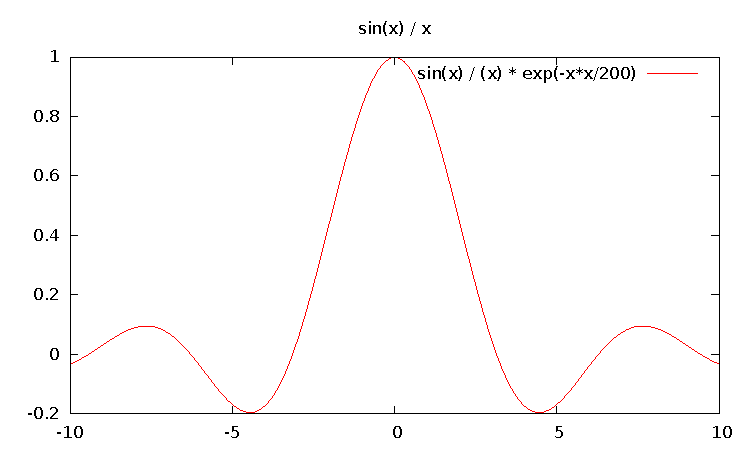
\includegraphics{Charts/pdf/PearsonRho.pdf}
%	\caption{pdf of the Distribution of the Sample Correlation Coefficient}
%	\label{Fig pdf of the Distribution of the Sample Correlation Coefficient}
%\end{figure}



\subsection{Density and CDF}

\begin{mpFunctionsExtract}
	\mpFunctionFourNotImplemented
	{PearsonRhoDist? mpNumList? pdf, CDF and related information for the distribution of the sample correlation coefficient}
	{x? mpNum? A real number}
	{N? mpNum? A real number greater 2, representing the sample size}
	{rho? mpNum? A real number greater 0, representing the correlation coefficient}
	{Output? String? A string describing the output choices}
\end{mpFunctionsExtract}


\vspace{0.3cm}
See section \ref{Functions returning pdf, CDF, and related information} for the options for {\itshape\sffamily Output}. Algorithms and formulas are given in sections \ref{rhoDistributionDensity} and \ref{rhoDistributionCDF}.

\subsubsection{Density: Hotelling's algorithm}
\nomenclature{$f_R(r, N; \rho)$}{pdf of the Distribution of the Sample Correlation Coefficient}
\label{rhoDistributionDensity}

We define
\begin{equation}  \label{eq:PearsonRho_Def_ABCU}
	x = \rho r,\quad \quad  A=\sqrt{1-\rho^2}, \quad B=\sqrt{1-x^2}, \quad C=\sqrt{1-r^2}, \quad U=\frac{\arccos(-x)}{B}
\end{equation}
The probability density function for $R$ is then given by \citep{hotelling_1953}
\begin{equation} \label{eq:PearsonRho_PDF_Ik_def}
	f_R(r, N; \rho) = K_1 A^{N-1} C^{N-4} (1-x)^{\tfrac{3}{2}-N}{}_2F_1\left(\tfrac{1}{2},\tfrac{1}{2}; N-\tfrac{1}{2}; \tfrac{1}{2}+\tfrac{1}{2}x\right),
\end{equation}
\begin{equation}  \label{eq:PearsonRho_K1}
	\text{where}  \quad  K_1 = \frac{(N-2)\Gamma(N-1)}{\sqrt{2\pi}\Gamma\left(N-\tfrac{1}{2}\right)},  
\end{equation}
\begin{equation}  \label{eq:PearsonRho_T1}
	{}_2F_1\left(\tfrac{1}{2},\tfrac{1}{2}; N-\tfrac{1}{2}; \tfrac{1}{2}+\tfrac{1}{2}x\right) =  \sum_{i=0}^{\infty} M_i,
\end{equation}
\begin{equation} 
	M_0= 1, \quad M_i = M_{i-1} \frac{a_i^2}{c_i} \frac{1+x}{2i}
\end{equation}
$a_1=\tfrac{1}{2}$, $c_1 = N-\tfrac{1}{2}$, $a_i=a_{i-1}+1$, $c_i=c_{i-1}+1$ and ${}_2F_1(\cdot)$ is the Gaussian hypergeometric function (see section \ref{sec:Hypergeometric2F1MpMath}).


\subsubsection{Density :Closed form expressions and recursions}
For $N = 3,4$ the probability density function can be expressed in closed form \citep{odeh_1986}:
\begin{equation}  \label{eq:PearsonRho_Closed_f3_density}
	f_R(r, 3; \rho) = \frac{A^2(1+xU)}{\pi B^2C} 
\end{equation}
\begin{equation} \label{eq:PearsonRho_Closed_f4_density}
	f_R(r, 4; \rho) =\frac{AC^3 (B^2U + 3x(1+xU))}{\pi B^4} 
\end{equation}
where $x, A, B, C$ and $U$ are defined in  (\ref{eq:PearsonRho_Def_ABCU}). The probability density function $f_N(r,\rho)$ satisfies the following recurrence formula for $N \geq 5$ \citep{hotelling_1953}:
\begin{equation} \label{eq:PearsonRho_PDF_Ik_recur}
	f_R(r, N; \rho) = \frac{2N-5}{B^2(N-3)} x A C f_R(r, N-1; \rho) + \frac{N-3}{B^2(N-4)} A^2 C^2 f_R(r, N-2; \rho)  
\end{equation}
For $0 \leq x \leq 1$, eqn (\ref{eq:PearsonRho_PDF_Ik_recur}) can be used to find a sequence of values for $f_5(r;\rho), f_6(r;\rho),...,f_{N}(r;\rho)$. However, for $-1 < x < 0$ the recurrence formula is numerically unstable, since the two terms on the right-hand of eqn  are of opposite sign. In this case $(1+x)<1$, so the series given by eqn (\ref{eq:PearsonRho_PDF_Ik_def}) will converge extremely fast and can be used.



\subsubsection{CDF: Hotelling's series}
\label{rhoDistributionCDF}
\citet{hotelling_1953}  defines $Q_N(r;\rho) = \text{Pr}[\rho<R<r]$ and develops  $Q_N(r;\rho)$ in the following uniformly convergent series for $-1<\rho<r<1$. 

\begin{equation}
	Q_N(r,\rho) = K_1 \sum_{j=0}^{\infty}{\frac{(1 \cdot 3 \cdots (2j-1))^2 S_j}{j! 2^{2j} \cdot (2N+1) \cdots (2N+2j-1)}},
\end{equation}
where $K_1$ and $S_j$ are defined in equations (\ref{eq:PearsonRho_K1}) and (\ref{eq:PearsonRho_Hotelling_Sj}), respectively. From the relationships
\begin{equation}
	P_N(r, \rho) = 1-F_R(r, N; \rho) = Q_N(1,\rho)-Q_N(r,\rho)
\end{equation}
\begin{equation}
	P_N(-1, \rho) = 1
\end{equation}
\begin{equation}
	F_R(r, N; \rho) = 1 -P_N(r, \rho)
\end{equation}
\begin{equation}
	F_R(-r, N; -\rho) = 1 -F_R(r, N; \rho)
\end{equation}
we can compute $F_N(r;\rho)$ for any value of r and $\rho$ with $-1 \leq r \leq 1$, $-1<\rho<1$.
Hotelling shows that the error committed by truncating the series at any point is less than $\frac{2}{1-|\rho|}$ times the last term used. However, it is important to note that the series converges very slowly for small values of $N$, and in this case a large number of terms must be computed.

\begin{equation}  \label{eq:PearsonRho_Hotelling_Sj}
	S_j = \sum_{k=0}^{j} \binom{j}{k}(-1)^k \: \tfrac{1}{2} (1-\rho^2)^k \: 2^{j-k}  N_k
\end{equation}
\begin{equation}
	N_k = \sum_{s=0}^{\infty} \frac{\Gamma\left(\tfrac{3}{2}-k\right)}{\Gamma\left(\tfrac{3}{2}-k-s\right) s!} \cdot I \left(\tfrac{1}{2}(s+1), \tfrac{1}{2}(n-1),\frac{(r-\rho)^2}{(1-\rho r)^2}\right),
\end{equation} 
where $I(a,b;x)$ denotes the Incomplete Beta Function (see section \ref{sec:IncompleteBetaFunction}). Hotelling shows that in the evaluation of $N_k$ for large $s$ the absolute value of the ratio of the term of order $(s+1)$ to the term of order $s$ is bounded by $|\rho (r-\rho)/(1-\rho r)|$, so that the series converges rapidly.


\subsubsection{CDF: Guenther's series}
\citet{guenther_pearson_rho_1977} writes $P_N(r;\rho) = \text{Pr}[R>0] -  \text{Pr}[0<R<r]$ and develops $\text{Pr}[0<R<r]$ in an infinite series involving the Incomplete Beta Function denoted by $I(a,b;x)$. The result is
\begin{equation}  \label{eq:PearsonRho_Guenther_1}
	\text{Pr}[R>0] = \tfrac{1}{2} \left[1+\text{sgn}(\rho) \cdot I\left(\tfrac{1}{2}(N-1), \tfrac{1}{2}; \rho^2\right) \right]
\end{equation}
\begin{IEEEeqnarray}{rCl} \label{eq:PearsonRho_Guenther_2}
	\text{Pr}[0 < R <r] & = \sum_{j=0}^{\infty} K_1(j) \cdot I\left(\tfrac{1}{2}(N-2), \tfrac{1}{2}(2j+1); r^2 \right) \\
	& + \sum_{j=0}^{\infty} K_2(j) \cdot I\left(\tfrac{1}{2}(N-2), j+1; r^2 \right)  \nonumber
\end{IEEEeqnarray}

where  $K_1(j), K_2(j)$ are defined recursively by

\begin{equation*}
	K_1(0) = \tfrac{1}{2} \left(1-\rho^2 \right)^{\tfrac{1}{2}(N-1)}, \quad K_1(j)=\frac{2j+N-3}{2j} \rho^2 K_1(j-1)
\end{equation*}
\begin{equation*}
	K_2(0) = \frac{\Gamma \left(\tfrac{1}{2}N\right)}{\sqrt{\pi}\Gamma\left(\tfrac{1}{2}(N-1)\right)} \rho \left(1-\rho^2 \right)^{\tfrac{1}{2}(N-1)}, \quad K_2(j)=\frac{2j+N-2}{2j+1} \rho^2 K_2(j-1)
\end{equation*}\\
Eqns (\ref{eq:PearsonRho_Guenther_1}) and (\ref{eq:PearsonRho_Guenther_2}) are used together to give $P_N(r;\rho)$. Guenther also obtains error bounds for truncating the infinite series given by (\ref{eq:PearsonRho_Guenther_2}).


\subsubsection{CDF: Closed form expressions and recursions}

For $N = 3,4,5,6$ the cdf can be expressed in closed form \citep{odeh_1986}:
\begin{equation}  \label{eq:PearsonRho_Closed_F3}
	F_3(r; \rho) = \frac{\arccos(-r)}{\pi} - \frac{\rho C U}{\pi}
\end{equation}
\begin{equation} \label{eq:PearsonRho_Closed_F4}
	F_4(r; \rho) =\frac{\arccos(\rho)}{\pi} - \frac{\rho AC^2}{\pi B^2} - \frac{rA^3U}{\pi B^2}
\end{equation}
\begin{equation} \label{eq:PearsonRho_Closed_F5}
	F_5(r; \rho) =\frac{\arccos(-r)}{\pi} - \frac{(x^2-3\rho^3+2) r A^2C}{2\pi B^4} + \frac{(\rho^2-3+2\rho^2 x^2) \rho C^3U}{2\pi B^4} 
\end{equation}
\begin{IEEEeqnarray}{rCl} \label{eq:PearsonRho_Closed_F6}
	F_6(r; \rho) & = &\frac{\arccos(\rho)}{\pi} - \frac{[\rho r^2(2x^2+13) - 2\rho(4x^4+6x^2+5) + \rho^3(11x^2+4)] AC^2}{6\pi B^6} \\
	&& + \frac{2x^2(-2r^2+1)rA^5U}{6\pi B^6}  \nonumber
\end{IEEEeqnarray}
where $x, A, B, C$ and $U$ are defined in  (\ref{eq:PearsonRho_Def_ABCU}). The cumulative distribution function $F_N(r,\rho)$ satisfies the following recurrence formula  for $N \geq 7$\citep{hotelling_1953}:
\begin{IEEEeqnarray}{rCl}  \label{eq:PearsonRho_Closed_Recur}
	F_{N}(r;\rho) & = & \frac{2 (N - 4) \rho^2 - N + 5}{(N-3)\rho^2} F_{N-2}(r;\rho) \\
	&& +\: \frac{(N-5)A^2}{(N-3)\rho^2} F_{N-4}(r;\rho) \nonumber \\
	&& +\: \frac{(N-4)A^2C^2-(2N-9) B^2}{(N-4)(N-3)\rho^2 AC} \rho f_{N-1}(r;\rho)  \nonumber \\
	&& +\: \frac{(N-4)^2 +(3N(N-8)+47)\rho^2}{(N-4)^2 (N-3)\rho^2} r f_{N-2}(r;\rho)    \nonumber 
\end{IEEEeqnarray}
For $N$ odd, the above formula can be used repeatedly to find $F_7, F_9, ..., F_N$ starting with values of $F_3$ and $F_5$, for which exact expressions are given by eqns (\ref{eq:PearsonRho_Closed_F3}) and  (\ref{eq:PearsonRho_Closed_F5}) respectively. For $N$ even, the formula can be used repeatedly to find $F_8, F_{10}, ..., F_N$ starting with values of $F_4$ and $F_6$, for which exact expressions are given by equations (\ref{eq:PearsonRho_Closed_F4}) and (\ref{eq:PearsonRho_Closed_F6}) respectively.
However, the formula can only be applied if $\rho^2 \geq \frac{N-5}{2(N-4)}$, since if $\rho^2$ is less then this bound, the first two terms on the right hand side of eqn (\ref{eq:PearsonRho_Closed_Recur}) are of opposite sign and the formula is numerically unstable.


\subsubsection{CDF: Fisher's Approximation}
The widely used Fisher $z$-transformation leads to the approximation
\begin{equation}
	F_N(r,\rho) \approx \Phi \left( \sqrt{N-3} \left(Z(r) - Z(\rho) \right) \right), \quad \text{where} 
\end{equation}
$Z(\cdot)$ is defined in equation  (\ref{eq:PearsonRho_zTransform}), and $\Phi(\cdot)$ denotes the CDF of the normal distribution (see section \ref{sec:NormalDistribution_CDF}). This approximation can be improved by using the first 4 cumulants of $Z(R)$, resulting in
\begin{equation}
	F_N(r,\rho) \approx \Phi \left(x \right), \quad \text{where}
\end{equation}
\begin{equation}
	u= \frac{Z(r) - \kappa_1}{\sqrt{\kappa_2}}, \quad x = u + (u^2 - 1) \frac{\gamma_1}{6} + (u^3 - 3 u) \frac{\gamma_2}{24} + (4 u^3 - 7u) \frac{\gamma_1^2}{36} 
\end{equation}
and $\kappa_1$, $\kappa_2$, $\gamma_1$ and $\gamma_2$ are defined in equations  (\ref{eq:PearsonRho_kappa1}) to  (\ref{eq:PearsonRho_gamma1}).

%
%\subsubsection{Winterbottom's Approximation DH}
%Particularly accurate results have been found by inverting Winterbottom's approximation for the confidence limits of $\rho$, (see section \ref{sec:Winterbottom_Approximation}), giving the following approximation to the CDF:
%\begin{equation}
%F_N(r,\rho) \approx \Phi \left(\frac{k}{6} - \frac{2c}{k} - \frac{b}{3}\right), \quad \text{where} \quad m = N - 1,
%\end{equation}
%\begin{equation*}
%a = \frac{1}{12\sqrt{m^3}} + \frac{6 r^4 - 3r^2 + 2}{48\sqrt{m^5}}, \quad  b = \frac{-r3}{6 a m^2}, \quad s=\frac{1}{a\sqrt{m}} + \frac{1+r^2}{4a\sqrt{m^3}} + \frac{11 r^4 - 2r^2 + 1}{32a\sqrt{m^5}} 
%\end{equation*}
%\begin{equation*}
%t = \frac{Z(r)-Z(\rho)}{a} + \frac{r}{2 a m} + \frac{5 r^3 + 9r}{24 a m^2}, \quad d=t+ \frac{bs}{3} - \frac{2b^3}{27}
%\end{equation*}
%\begin{equation*}
%c = s-b^2/3, \quad p=\sqrt{|12c^3+81d^2|}, \quad k=(108d+12p)^{1/3}
%\end{equation*}
%$Z(\cdot)$ is defined in equation  (\ref{eq:PearsonRho_zTransform}), and $\Phi(\cdot)$ denotes the CDF of the normal distribution (see section \ref{sec:NormalDistribution_CDF}).
%





\subsubsection{CDF: Winterbottom's Approximation}
\label{sec:Winterbottom_Approximation_CDF}
The CDF approximation given by \citep{winterbottom_1980} is:
\begin{equation}
	F_N(r,\rho) \approx \Phi \left(\sqrt{m}Y \right), \quad \text{where} \quad m=N-1,
\end{equation}
\begin{IEEEeqnarray}{rCl}
	Y & = & - \frac{r}{2m} - \frac{3r+r^3}{12m^2} + \left( 1 - \frac{1+r^2}{4m} + \frac{3 - 11r^4}{96m^2} \right) w \\
	&& +\:  \frac{3r-4r^3}{24m} w^2 - \left( \frac{1}{12} - \frac{2 + 7r^2- 6r^4}{48m} \right) w^3 + \frac{3}{160} w^5,  \nonumber 
\end{IEEEeqnarray}
$w = Z(r)-Z(\rho)$  and $Z(\cdot)$ is defined in equation  (\ref{eq:PearsonRho_zTransform}).







\subsection{Quantiles}


\begin{mpFunctionsExtract}
	\mpFunctionFourNotImplemented
	{PearsonRhoDistInv? mpNumList? quantiles and related information for the distribution of the sample correlation coefficient}
	{Prob? mpNum? A real number between 0 and 1.}
	{N? mpNum? A real number greater 2, representing the sample size}
	{rho? mpNum? A real number greater 0, representing the correlation coefficient}
	{Output? String? A string describing the output choices}
\end{mpFunctionsExtract}


\vspace{0.3cm}
For a given value of $\alpha, N$ and $\rho$ a $100\alpha$ percentage point of $R$ is the unique value of $R$, say $r_\alpha$, which satisfies $F_N(r_\alpha; \rho) = \alpha$

Let $u_\alpha$ = $\Phi^{-1}(\alpha)$ be the lower $100\alpha$ percentage point of the standard normal distribution (see section \ref{sec:NormalDistribution_Quantiles}). Then an approximation to the $100\alpha$ percentage point $r_\alpha$ is obtained by

\begin{equation}
	r_\alpha \approx Z^{-1}\left(Z(\rho)+\frac{u_{\alpha}}{\sqrt{N-3}}\right).
\end{equation}
$Z(\cdot)$  and $Z^{-1}(\cdot)$ are defined in equations  (\ref{eq:PearsonRho_zTransform}) and  (\ref{eq:PearsonRho_Inverse_zTransform}). This approximation can be improved by using the first 4 cumulants of $Z(R)$, resulting in
\begin{equation}
	r_\alpha \approx Z^{-1}\left(\kappa_1+x \sqrt{\kappa_2}\right) \quad \text{where} 
\end{equation}
\begin{equation}
	x = u_\alpha + (u_\alpha^2 - 1) \frac{\gamma_1}{6} + (u_\alpha^3 - 3 u_\alpha) \frac{\gamma_2}{24} + (2 u_\alpha^3 - 5u_\alpha) \frac{\gamma_1^2}{36} 
\end{equation}
and $\kappa_1$, $\kappa_2$, $\gamma_1$ and $\gamma_2$ are defined in equations  (\ref{eq:PearsonRho_kappa1}) to  (\ref{eq:PearsonRho_gamma1}).



\subsubsection{Winterbottom's Quantile Approximation}
\label{sec:Winterbottom's Quantile Approximation}
An approximation to the $100\alpha$ percentage point $r_\alpha$ is obtained by \citep{winterbottom_1980}
\begin{equation}
	r_\alpha \approx Z^{-1}(y), \quad \text{where }
\end{equation}
\begin{IEEEeqnarray}{rCl}
	y & = & Z(\rho) + \frac{u_\alpha}{\sqrt{m}} + \frac{\rho}{2m} + \frac{u_\alpha^3+3(3-\rho^2)u_\alpha}{12\sqrt{m^3}} + \frac{4\rho^3 u_\alpha^2 + 15\rho-\rho^3}{24m^2} \\
	&& +\: \frac{u_\alpha^5+(-60\rho^4+30\rho^2+80)u_\alpha^3 + (45\rho^4-21\rho^2+375)u_\alpha}{480\sqrt{m^5}}   \nonumber  
\end{IEEEeqnarray}
$Z(\cdot)$  and $Z^{-1}(\cdot)$ are defined in equations  (\ref{eq:PearsonRho_zTransform}) and  (\ref{eq:PearsonRho_Inverse_zTransform}).





\subsection{Properties}
\label{rhoDistributionProperties}

\begin{mpFunctionsExtract}
	\mpFunctionThreeNotImplemented
	{PearsonRhoDistInfo? mpNumList? moments and related information for the distribution of the sample correlation coefficient}
	{N? mpNum? A real number greater 2, representing the sample size}
	{rho? mpNum? A real number greater 0, representing the correlation coefficient}
	{Output? String? A string describing the output choices}
\end{mpFunctionsExtract}

\vspace{0.3cm}

See section \ref{Functions returning moments and related information} for the options for {\itshape\sffamily Output}. Algorithms and formulas are given below.



\subsubsection{The moments of $R$}
The moments of $R$ are given by \cite{Anderson_book_2003}, p. 166:
\begin{equation}
	\mathbb{E}\left(R^{2h+1}\right) = \frac{(1-\rho^2)^{n/2}}{\sqrt{\pi} \Gamma(n/2)} \sum_{i=0}^{\infty} {\frac{(2\rho)^{2i+1}}{(2i+1)!} \frac{\Gamma^2[(n+1)/2+i] \Gamma(h+i+3/2)}{\Gamma(n/2 +h+i+1)}   }
\end{equation}
\begin{equation}
	\mathbb{E}\left(R^{2h}\right) = \frac{(1-\rho^2)^{n/2}}{\sqrt{\pi} \Gamma(n/2)} \sum_{i=0}^{\infty} {\frac{(2\rho)^{2i}}{(2i)!} \frac{\Gamma^2[(n+1)/2+i] \Gamma(h+i+1/2)}{\Gamma(n/2 +h+i)}   }
\end{equation}
The first 4 moments of the distribution of $R$ can also be expressed in terms of hypergeometric functions (see \cite{Johnson_1995} p.553):
%\begin{equation}
%\mu'_1= c_n \rho \times {}_2F_1\left(\tfrac{1}{2},\tfrac{1}{2};\tfrac{1}{2}(n+1);\rho^2 \right)
%\end{equation}
%\begin{equation}
%\mu'_2= 1 - \frac{(n-2)(1-\rho^2)}{n-1} \times {}_2F_1\left(1,1;\tfrac{1}{2}(n+1);\rho^2 \right)
%\end{equation}
%\begin{IEEEeqnarray}{rCl}
%\mu'_3 & = & c_n \left[ \rho \times {}_2F_1\left(\tfrac{1}{2},\tfrac{1}{2};\tfrac{1}{2}(n+1);\rho^2 \right) - \frac{(n-1)(n-2)}{\rho} \right] \\
%&& \times \: \left[{}_2F_1\left(\tfrac{1}{2},\tfrac{1}{2};\tfrac{1}{2}(n-1);\rho^2 \right) -  {}_2F_1\left(\tfrac{1}{2},\tfrac{1}{2};\tfrac{1}{2}(n+1);\rho^2 \right) \right] \nonumber  
%\end{IEEEeqnarray}
%\begin{IEEEeqnarray}{rCl}
%\mu'_4 & = &  1 + \frac{(n-2)(n-4)(1-\rho^2)}{2(n-1)} \times {}_2F_1\left(1,1;\tfrac{1}{2}(n+1);\rho^2 \right) \\
%&& - \:  \frac{n(n-2)(n-\rho^2)}{4\rho^2} \left[{}_2F_1\left(1,1;\tfrac{1}{2}(n+1);\rho^2 \right)-1\right] \nonumber  
%\end{IEEEeqnarray}

\begin{equation}
	\mu'_1 = c_n b_1 \rho
\end{equation}
\begin{equation}
	\mu'_2= 1 - \frac{b_2(n-2)(1-\rho^2)}{n-1}
\end{equation}
\begin{equation}
	\mu'_3= c_n  (b_3-b_1) \left(b_1 \rho - \frac{(n-1)(n-2)}{\rho} \right)
\end{equation}
\begin{equation}
	\mu'_4=  1 + \frac{b_2(n-2)(n-4)(1-\rho^2)}{2(n-1)} - \frac{(b_2 - 1)n(n-2)(n-\rho^2)}{4\rho^2} 
\end{equation}
with
\begin{equation}
	c_n = \frac{2}{n-1} \left[\frac{\Gamma(n/2)}{\Gamma((n-1)/2)}\right]^2
\end{equation}
\begin{equation}
	b_1 = {}_2F_1\left(\tfrac{1}{2},\tfrac{1}{2};\tfrac{1}{2}(n+1);\rho^2 \right)
\end{equation}
\begin{equation}
	b_2 = {}_2F_1\left(1,1;\tfrac{1}{2}(n+1);\rho^2 \right)
\end{equation}
\begin{equation}
	b_3 = {}_2F_1\left(\tfrac{1}{2},\tfrac{1}{2};\tfrac{1}{2}(n-1);\rho^2 \right)
\end{equation}
where $\Gamma(\cdot)$ is the Gamma function (see section \ref{GammaFunction}), and ${}_2F_1(\cdot)$ is the Gaussian hypergeometric function (see section \ref{sec:Hypergeometric2F1MpMath}).


\subsubsection{Fisher's z-transform}
The Fisher $z$-transform is defined by
\begin{equation}  \label{eq:PearsonRho_zTransform}
	Z(a)=\tfrac{1}{2} \log \left(\frac{1+a}{1-a}\right) = \text{atanh}(a)
\end{equation}

The inverse Fisher $z$-transform is defined by
\begin{equation} \label{eq:PearsonRho_Inverse_zTransform}
	Z^{-1}(a) = \frac{e^{2a}-1}{e^{2a}+1} = \tanh(a)
\end{equation}




\subsubsection{The cumulants of $Z(R)$}
Let $m = N - 1$. Then the first 4 cumulants of $Z(R)$ (with $Z(\cdot)$as defined in equation \ref{eq:PearsonRho_zTransform}) are given by \citep{hotelling_1953}
\begin{equation} \label{eq:PearsonRho_kappa1}
	\kappa_1= \tfrac{1}{2} \log \left(\frac{1+\rho}{1-\rho}\right) + \frac{\rho}{2m} + \frac{5+\rho^2}{4m^2} + \frac{11+2\rho^2+3\rho^4}{8m^3} + O(m^{-4})
\end{equation}
\begin{equation}
	\kappa_2=\frac{1}{m} + \frac{4-\rho^2}{2m^2} + \frac{22-6\rho^2-3\rho^4}{6m^3} + O(m^{-4})
\end{equation}
\begin{equation}
	\kappa_3=\frac{\rho^3}{m^3} + O(m^{-4})
\end{equation}
\begin{equation}
	\kappa_4=\frac{2}{m^3} + O(m^{-4})
\end{equation}
\begin{equation}  \label{eq:PearsonRho_gamma1}
	\gamma_1=\frac{\kappa_3}{\sqrt{\kappa_2}\kappa_2}, \quad \gamma_2=\frac{\kappa_4}{\kappa_2^2} 
\end{equation}



\subsection{Random Numbers}
\label{PearsonRhoDistributionRandom}

\begin{mpFunctionsExtract}
	\mpFunctionFiveNotImplemented
	{PearsonRhoDistRan? mpNumList? random numbers following the distribution of the sample correlation coefficient}
	{Size? mpNum? A positive integer up to $10^7$}
	{N? mpNum? A real number greater 2, representing the sample size}
	{rho? mpNum? A real number greater 0, representing the correlation coefficient}
	{Generator? String? A string describing the random generator}
	{Output? String? A string describing the output choices}
\end{mpFunctionsExtract}


\vspace{0.3cm}
See section \ref{Functions returning Random numbers} for the options for  {\itshape\sffamily Size},  {\itshape\sffamily Generator} and {\itshape\sffamily Output}. Algorithms and formulas are given below:


\vspace{0.3cm}
The correlation coefficient $r$ in samples of size $N>2$ from a non-singular bivariate normal population with correlation coefficent $\rho$ can be represented in the form
\begin{equation}
	\tilde{r} = \frac{z+ \tilde{\rho} \chi_{N-1}}{\chi_{N-2}}
\end{equation}
where $\tilde{r} =r/\sqrt{1-r^2}$ , $\tilde{\rho} =\rho/\sqrt{1-\rho^2}$, $z$ is a standardized normal variate and  $z$ , $\chi_{N-1}$, and $\chi_{N-2}$ are independent \citep{ruben_1966}. This can be used to develop an approximation where
\begin{equation}
	\frac{\sqrt{(2N-5)/2} \tilde{r} - \sqrt{(2N-3)/2} \tilde{\rho}}{\sqrt{1+ \tfrac{1}{2}( \tilde{r}^2+\tilde{\rho}^2)}}
\end{equation}
is distributed as a standard normal variate. See also \cite{akahira_1998}.







\subsection{Confidence limits for rho}
\label{PearsonRhoDistributionNC}


\begin{mpFunctionsExtract}
	\mpFunctionFourNotImplemented
	{PearsonRhoDistNoncentrality? mpNumList? confidence limits for the noncentrality parameter rhi and related information for the distribution of the sample correlation coefficient.}
	{alpha? mpNum? A real number between 0 and 1, specifies the confidence level (or Type I error).}
	{rho? mpNum? A real number between -1 and 1, representing the noncentrality parameter.}
	{N? mpNum? A real number greater 2, representing the sample size}
	{Output? String? A string describing the output choices}
\end{mpFunctionsExtract}


\vspace{0.3cm}
See section \ref{Functions related to noncentrality parameters} for the options for  {\itshape\sffamily alpha}, {\itshape\sffamily Noncentrality} and {\itshape\sffamily Output}. Algorithms and formulas are given below.

\vspace{0.3cm}
For a given value of $\alpha_1<\tfrac{1}{2}$, $N$, and an observed value of $R$, say $r_0$, a lower $100(1-\alpha_1)\%$ confidence limit on $\rho$ is the unique value of $\rho$, say $\rho_L$, which satisfies $F_N(r_0; \rho) = 1-\alpha_1$. A one-sided lower  $100(1-\alpha_1)\%$ confidence interval on $\rho$ is given by $\rho_L \leq \rho \leq 1$.

For $\alpha_1<\tfrac{1}{2}$, an upper $100(1-\alpha_2)\%$ confidence limit on $\rho$ is the unique value of $\rho$, say $\rho_U$, which satisfies $F_N(r_0; \rho) = 1-\alpha_2$. A one-sided upper $100(1-\alpha_2)\%$ confidence interval on $\rho$ is given by  $-1 \leq \rho \leq \rho_U$.

For $\alpha_1=1-\alpha_2=\alpha_0$, an equal-tailed two-sided  $100(1-2\alpha_0)\%$ confidence interval on $\rho$ is given by  $\rho_L \leq \rho \leq \rho_U$.


\subsubsection{Fisher's Approximation}
To obtain a confidence interval for ρ, we first compute a confidence interval for z(r). The inverse Fisher transformation bring the interval back to the correlation scale.
\begin{equation}
	\rho_L \approx Z^{-1}\left(Z(r)- \frac{u_{\alpha}}{\sqrt{N-3}}\right).
\end{equation}
For example, suppose we observe r = 0.3 with a sample size of n=50, and we wish to obtain a 95\% confidence interval for $\rho$. The transformed value is arctanh(0.3) = 0.30952, so the confidence interval on the transformed scale is $0.30952 - 1.96/\sqrt{47}$, or (0.023624, 0.595415). Converting back to the correlation scale yields (0.024, 0.534).

\subsubsection{Winterbottom's Approximation}
\label{sec:Winterbottom_Approximation}
Let $u_\alpha$ = $\Phi^{-1}(\alpha)$ be the lower $100\alpha$ percentage point of the standard normal distribution (see section \ref{sec:NormalDistribution_Quantiles}) and let $m=N-1$. Then an asymptotic approximation for a lower $100(1-\alpha)$ confidence limit on $\rho$ is given by \citep{winterbottom_1980}
\begin{equation}
	\rho_L \approx Z^{-1}(y), \quad \text{where }
\end{equation}
\begin{IEEEeqnarray}{rCl}
	y & = & Z(r) + \frac{u_\alpha}{\sqrt{m}} - \frac{r}{2m} + \frac{u_\alpha^3+3(1+r^2)u_\alpha}{12\sqrt{m^3}} - \frac{4r^3 u_\alpha^2 + 5r^3+9r}{24m^2} \\
	&& +\: \frac{u_\alpha^5+(60r^4-30r^2+20)u_\alpha^3 + (165r^4+30r^2+15)u_\alpha}{480\sqrt{m^5}}   \nonumber  
\end{IEEEeqnarray}
$Z(\cdot)$  and $Z^{-1}(\cdot)$ are defined in equations  (\ref{eq:PearsonRho_zTransform}) and  (\ref{eq:PearsonRho_Inverse_zTransform}).




\subsection{Sample Size Function}
\nomenclature{$N_{Rho}\left(\alpha, \beta, \widetilde{\rho} \right)$}{Sample size function of the noncentral $t$-distribution for a given confidence level $\alpha$, power $\beta$ and modified noncentrality parameter $\widetilde{\rho}$}
\label{PearsonRhoDistributionSampleSize}

\begin{mpFunctionsExtract}
	\mpFunctionFourNotImplemented
	{PearsonRhoDistSampleSize? mpNumList? sample size estimates and related information for the distribution of the sample correlation coefficient.}
	{alpha? mpNum? A real number between 0 and 1, specifies the confidence level (or Type I error).}
	{beta? mpNum?  A real number between 0 and 1, specifies the Type II error (or 1 - Power).}
	{ModifiedNoncentrality? mpNum? A real number greater 0, representing the modified noncentrality parameter.}
	{Output? String? A string describing the output choices}
\end{mpFunctionsExtract}

\vspace{0.3cm}
See section \ref{Functions returning Sample Size estimates} for the options for  {\itshape\sffamily alpha}, {\itshape\sffamily beta}, {\itshape\sffamily ModifiedNoncentrality} and {\itshape\sffamily Output}. Algorithms and formulas are given below.

\vspace{0.3cm}
We denote by $N_{Rho}\left(\alpha, \beta, \widetilde{\rho} \right)$  the sample size function of the noncentral $t$-distribution for a given confidence level $\alpha$, power $\beta$ and modified noncentrality parameter $\widetilde{\rho}$. This function determines the minimal sample size $N$ for given noncentrality parameter, Type I error $1-\alpha$, and Type II error $1-\beta$, where  $\delta = \sqrt{N}\widetilde{\rho}$ 





\newpage
\section{Distribution of the Sample Multiple Correlation Coefficient}
\label{Rho2Distribution}



\subsection{Definition}
\label{Rho2DistributionDefinition}

Let $(X_1, \ldots, X_N)$ be a sample of independent vector observations from a  $p$-variate normal population with mean $\boldsymbol{\mu}$ and covariance matrix $\boldsymbol{\Sigma}$. Define
\begin{equation}
	\overline{X} = \frac{1}{N} \sum_{i=1}^N X_i \quad and \quad \textbf{A} = \sum_{i=1}^N (X_i - \overline{X}) (X_i - \overline{X})'.
\end{equation}
Partition $\textbf{A}$ as
\begin{equation}
	\textbf{A} =
	\begin{pmatrix}
		a_{11} & \textbf{a}_{12} \\
		\textbf{a}_{21} & \textbf{A}_{22} 
	\end{pmatrix}
\end{equation}
so that $a_{11}$ is $1 \times 1$, $\textbf{a}_{12}$ is $1 \times (p-1)$, and $\textbf{A}_{22}$ is a $(p-1) \times (p-1)$ matrix. In terms of these submatrices, the squared sample multiple correlation coefficient is given by

\begin{equation}
	R^2 = \frac{\textbf{a}_{12} \textbf{A}_{22}^{-1} \textbf{a}_{21}}{a_{11}}
\end{equation}
The sample multiple correlation coefficient is the positive square root of $R^2$. The squared population multiple correlation coefficient, $\rho^2$, is defined similarly in terms of the submatrices of $\boldsymbol{\Sigma}$.

For given $N-p \geq 1$, the distribution of $R^2$ is independent of $\boldsymbol{\mu}$ and $\boldsymbol{\Sigma}$, but depends upon  $\rho^2$, where $0 \leq \rho^2 < 1$.
For $0 \leq x \leq 1$, define $f_{R^2}(x;p,N,\rho^2)$ to be the probability density function for $R^2$. We denote the cumulative distribution function of $R^2$ by

\begin{equation}
	F_{R^2}(x;p,N,\rho^2) = \text{Pr}[R^2 \leq x] = \int_{0}^{x}{f_{R^2}(t;p,N,\rho^2)) dt}.
\end{equation}


Note: The univariate version of the noncentral distribution of Wilks $\Lambda$: Canonical Correlation 
(see section \ref{WilksLambdaDistributionDefinition_CORR})
is equivalent to $W=1-R^2$.




\subsection{Density and CDF}

\begin{mpFunctionsExtract}
	\mpFunctionFiveNotImplemented
	{Rho2Dist? mpNumList? pdf, CDF and related information for the distribution of the squared population multiple correlation coefficient}
	{x? mpNum? A real number}
	{p? mpNum? An integer greater 2, representing the number of variates}
	{N? mpNum? A real number greater p, representing the sample size}
	{Rho2? mpNum? A real number greater or equal 0, representing the squared sample multiple correlation coefficient}
	{Output? String? A string describing the output choices}
\end{mpFunctionsExtract}



\subsubsection{Density: Infinite series}
\nomenclature{$f_{R^2}(x;p,n,\rho^2)$}{pdf of the Square of the Multiple Sample Correlation Coefficient}
\label{Rho2DistributionDensity}

The density function of the multiple sample correlation coefficient is given by \citep{Ding_1996,Benton_2003}
\begin{equation}
	f_{R^2}(x;p,N,\rho^2) = \sum_{i=0}^\infty f_{\text{NegBin}}\left((N-1)/2, i; 1-\rho^2\right) \times f_{\text{Beta}}\left(x; \tfrac{1}{2}(p-1) + i, \tfrac{1}{2}(N-p)\right)
\end{equation}
where $f_{\text{NegBin}}(\cdot)$ denotes the pmf of the negative binomial distribution (see section \ref{NegativBinomialDistributionDensity}) and $f_{\text{Beta}}(\cdot)$ denotes the pdf of the Beta distribution (see section \ref{BetaDistributionDensity})


\subsubsection{Density: Representation in terms of hypergeometric functions}
The density function of the multiple sample correlation coefficient is given by \citep{lee_results_1971,gurland_1968}
\begin{equation}
	f_{R^2}(x;p,n,\rho^2) = \frac{(1-\rho^2)^{n/2} (x)^{(n_1-2)/2} (1-x)^{(n_2-2)/2} {}_2F_1(\tfrac{1}{2}n, \tfrac{1}{2}n, \tfrac{1}{2}n_1; \rho^2 x)}{B(\tfrac{1}{2}n_1,\tfrac{1}{2}n_2 )}
\end{equation}

\begin{equation}
	f_{R^2}(x;p,N,\rho^2) = f_{Beta}\left(x; \tfrac{1}{2}(p-1), \tfrac{1}{2}(N-p)\right) (1-\rho^2)^{n/2} \times {}_2F_1(\tfrac{1}{2}N, \tfrac{1}{2}N, \tfrac{1}{2}p; \rho^2 x)
\end{equation}
where $f_{\text{Beta}}(\cdot)$ denotes the pdf of the Beta distribution (see section \ref{BetaDistributionDensity}) 
and ${}_2F_1(\cdot)$ is the Gaussian hypergeometric function (see section \ref{sec:Hypergeometric2F1MpMath}).

\subsubsection{Density: Closed form expressions for odd $p$}
For the particular cases of $p=3$ and $p=5$, we have for the pdf \citep{lee_results_1971}:
\begin{equation}
	f_{R^2}(n,3;\rho^2)  = \frac{ (n-3)\sqrt{1-\rho^2} \left[f_{R}(n-1,R;\rho) - f_{R}(n-1,-R;\rho)\right] }{2(n-2)\rho\sqrt{1-R^2}}
\end{equation}

\begin{IEEEeqnarray}{rCl} 
	f_{R^2}(n,5;\rho^2) & = & \frac{ (n-5)(1-\rho^2)R \left[f_{R}(n-2,R;\rho) + f_{R}(n-2,-R;\rho)\right]}{2(n-2)\rho^2(1-R^2)} \\
	& - & \frac{2(1-\rho^2)(1-R^2) f_{R^2}(n-2,3;\rho^2)}{2(n-2)\rho^2(1-R^2)}  \nonumber
\end{IEEEeqnarray}
where $f_{R}(\cdot)$ denotes the pdf of the distribution of the sample correlation coeffcient (see section \ref{rhoDistributionDensity}).
Starting with these formulas, the pdf can be calculated for all odd $p$, using the recurrence relation given in equation (\ref{eq:RecurrenceR2pdf}).




\subsubsection{CDF: Infinite series}
\nomenclature{$F_{R^2}(x;p,n,\rho^2)$}{CDF of the Square of the Multiple Sample Correlation Coefficient}
The CDF of the multiple sample correlation coefficient is given by \citep{Ding_1996,Benton_2003}
\begin{equation}
	F_{R^2}(x;p,N,\rho^2) = \sum_{i=0}^\infty f_{\text{NegBin}}\left((N-1)/2, i; 1-\rho^2\right) \times  F_{\text{Beta}}\left(x; \tfrac{1}{2}(p-1) + i, \tfrac{1}{2}(N-p)\right)
\end{equation}
where $f_{\text{NegBin}}(\cdot)$ denotes the pmf of the negative binomial distribution and $F_{\text{Beta}}(\cdot)$ denotes the CDF of the Beta distribution (see section \ref{BetaDistributionCDF})
where $f_{\text{NegBin}}(\cdot)$ denotes the pmf of the negative binomial distribution (see section \ref{NegativBinomialDistributionDensity}) and $F_{\text{Beta}}(\cdot)$ denotes the CDF of the Beta distribution (see section \ref{BetaDistributionCDF})


\subsubsection{CDF: Series of Gurland}
Let $R^2$ be the sample multiple correlation coefficent between $X$ (consisting of $p-1$ variates) and $Y$, based on $N$ observations. If both $X$ and $Y$ are random variates, then 
distribution of $F$ is given by \citep{lee_tables_1972,Gurland_1970}, 
\begin{equation}
	\text{Pr}[F \leq x] = F_{R^2}(x;a,b,\rho^2) = \frac{b^m}{a^{n/2}}  \sum_{j=0}^{\infty}{c_j I(m+j,k,y)} \quad \text{where}
\end{equation}
\begin{equation*}
	z=F(p-1), \quad y=\frac{z}{z+(N-p)}, \quad a=\frac{1}{1-\rho^2}, \quad n=(N-p)/2, \quad m=(p-1)/2
\end{equation*}
\begin{equation*}
	c_0=1, \quad c_j=\frac{c_{j-1}(-n/2-j+1)\rho^2}{j}
\end{equation*}


\subsubsection{CDF: Closed form expressions for odd $p$}
For the particular cases of $p=3$ and $p=5$, we have for the CDF \citep{lee_results_1971}:
\begin{equation}
	F_{R^2}(n,3;\rho^2) = F_{R^2}(n,1;\rho^2) - \frac{\sqrt{(1-\rho^2)(1-R^2)}\left[f_{R}(n-1,R;\rho) - f_{R}(n-1,-R;\rho)\right] }{(n-2)\rho}
\end{equation}

\begin{IEEEeqnarray}{rCl} 
	F_{R^2}(n,5;\rho^2) &=& F_{R^2}(n,3;\rho^2) - \frac{(1-\rho^2)R \left[f_{R}(n-2,R;\rho) - f_{R}(n-2,-R;\rho)\right] }{(n-2)\rho} \quad \quad \\
	& - & \frac{(1-\rho^2) \left[F_{R^2}(n-2,3;\rho^2) - F_{R^2}(n-2,1;\rho^2) \right]}{(n-2)\rho}  \nonumber
\end{IEEEeqnarray}
where $F_{R}(\cdot)$ denotes the CDF of the distribution of the sample correlation coeffcient (see section \ref{rhoDistributionCDF}).
Starting with these formulas, the CDF can be calculated for all odd $p$, using the recurrence relation given in equation (\ref{eq:RecurrenceR2CDF}).


\subsubsection{CDF: Approximation by non-central F}
\cite{lee_results_1971} suggests the following approximation, based on the noncentral $F$ distribution:
\begin{equation}
	F_{R^2}(x;n_1,n_2,\rho^2) \thickapprox F_{F'}\left(y; \nu, n_2, \lambda\right), \quad \text{where}
\end{equation}
\begin{center}
	
	$\gamma=1/(1-\rho^2)$, 
	
	\vspace{0.3cm}
	$A_j=(n_1+n_2) (\gamma^{\:j}-1) + n_1, \quad j=1,2,3, $
	
	\vspace{0.3cm}
	$G = (A_2 - \sqrt{A_2^2  -A_1 A_3})/A_1$, 
	
	\vspace{0.3cm}
	$\lambda=\rho^2 \gamma \sqrt{\gamma (n_1+n_2) n_2}/G^2 $,
	
	\vspace{0.3cm}
	$\nu= (A_2/G^2)- 2\lambda$, 
	
	\vspace{0.3cm}
	$y= x/(1-x) \times n_2/(\nu \cdot G)$, 
	
\end{center}

and $F_{F'}\left(\cdot; \nu, n_2, \lambda\right)$ denotes the CDF of the noncentral $F$ distribution with $\nu$ and $n_2$ degrees of freedom and noncentrality parameter $\lambda$ 
%(see section \ref{NoncentralFDistributionCDFBoost})
. For performance reasons, the noncentral $F$ distribution is evaluated using the (fast and highly accurate) saddlepoint approximation given in section \ref{NoncentralFDistributionCDFSaddlepoint}, rather than any of the "exact" algorithms.




\subsubsection{CDF: 2-moment approximation by central F}
\begin{equation}
	F_{F'}(x;n_1,n_2,\rho^2)  \thickapprox  F_F\left(x/c; m_1, n_2\right), 
\end{equation}
where $c=A_1/n_1$, $m_1= A_1^2/A_2$, $A_1=(n_1+n_2) (\gamma-1)+n_1$, $A_2=(n_1+n_2) (\gamma^2-1)+n_1$, $\gamma=1/(1-\rho^2)$, and $F_F\left(\cdot; m_1, n_2\right)$ denotes the CDF of a central $F$ distribution with $m_1$ and $n_2$ degrees of freedom (see \ref{FDistributionCDF}.






\subsection{Quantiles}

\begin{mpFunctionsExtract}
	\mpFunctionFiveNotImplemented
	{Rho2DistInv? mpNumList? quantiles and related information for the distribution of the squared population multiple correlation coefficient}
	{Prob? mpNum? A real number between 0 and 1.}
	{p? mpNum? An integer greater 2, representing the number of variates}
	{N? mpNum? A real number greater p, representing the sample size}
	{Rho2? mpNum? A real number greater or equal 0, representing the squared sample multiple correlation coefficient}
	{Output? String? A string describing the output choices}
\end{mpFunctionsExtract}

See section \ref{Functions returning Quantiles} for the options for  {\itshape\sffamily Prob} and {\itshape\sffamily Output}). Algorithms and formulas are given below.



\vspace{0.3cm}
An approximation to $Rho^2_{\alpha,n_1,n_2,\lambda} $, the $\alpha$-quantile of the distribution of the squared population multiple correlation coefficient with $p$ variates, sample size $N$ the distribution of the squared population multiple correlation coefficient and noncentrality parameter $\rho^2$, is obtained as
\begin{equation}
	F_{\alpha,n_1,n_2,\lambda}  \thickapprox  c \cdot F_{\alpha,m_1,n_2,} 
\end{equation}
where $c=A_1/n_1$, $m_1= A_1^2/A_2$, $A_1=(n_1+n_2) (\gamma-1)$, $A_2=(n_1+n_2) (\gamma^2-1)$, $\gamma=1/(1-\rho^2)$, and $F_{\alpha,m_1,n_2}$ denotes the $\alpha$-quantile of a central $F$-distribution with $m_1$ and $n_2$ degress of freedom (see section \ref{FINV}). 




\subsection{Properties}
\label{Rho2DistributionProperties}

\begin{mpFunctionsExtract}
	\mpFunctionFourNotImplemented
	{Rho2DistInfo? mpNumList? moments and related information for the distribution of the squared population multiple correlation coefficient}
	{p? mpNum? An integer greater 2, representing the number of variates}
	{N? mpNum? A real number greater p, representing the sample size}
	{Rho2? mpNum? A real number greater or equal 0, representing the squared sample multiple correlation coefficient}
	{Output? String? A string describing the output choices}
\end{mpFunctionsExtract}

\vspace{0.3cm}

See section \ref{Functions returning moments and related information} for the options for {\itshape\sffamily Output}. Algorithms and formulas are given below.



\subsubsection{Recurrence relations}
\cite{lee_results_1971} gives the following recurrence relations for the pdf and CDF, valid for all integer values of $p \geq 6$:
\begin{IEEEeqnarray}{rCl} \label{eq:RecurrenceR2pdf}
	(n-2)\rho^2(1-R^2) f_{R^2}(n,p;\rho^2) & = & (n-p)R^2(1-\rho^2) f_{R^2}(n-2,p-4;\rho^2) \\
	& - &  (p-4)(1-\rho^2)(1-R^2)  f_{R^2}(n-2,p-2;\rho^2)  \nonumber
\end{IEEEeqnarray}
\begin{IEEEeqnarray}{rCl} \label{eq:RecurrenceR2CDF}
	(n-2)\rho^2(1-R^2) F_{R^2}(n,p;\rho^2) & = & (n-p)\rho^2 F_{R^2}(n,p-2;\rho^2) \\
	& - &  (p-4)(1-\rho^2) \left[F_{R^2}(n-2,p-2;\rho^2) - F_{R^2}(n-2,p-4;\rho^2) \nonumber  \right]\\
	& - &  2R^2(1-\rho^2) f_{R^2}(n-2,p-4;\rho^2)  \nonumber
\end{IEEEeqnarray}


\subsubsection{The moments of $R^2$}
\label{MomentsR2}
\cite{Muirhead_1982}, p. 178, gives the following formula (see also \cite{Johnson_1995}, p. 621)
\begin{equation}
	\mathbb{E}[(1-R^2)^h] = \frac{\left[\tfrac{1}{2}(n-m+1)\right]_h}{\left(\tfrac{1}{2}n\right)_h} (1-\bar{R}^2)^h \times {}_2F_1(h,h,\tfrac{1}{2}n+h;\bar{R}^2).
\end{equation}
where $(a)_k$ is the Pochammer symbol (see section \ref{PochhammerSymbol}) and ${}_2F_1(\cdot)$ is the Gaussian hypergeometric function (see section \ref{sec:Hypergeometric2F1MpMath}).


The lower order moments are given by
\begin{equation}
	\mu'_1 = 1 - \frac{(n-m+1)}{n} (1-\bar{R}^2)^h \times {}_2F_1(1,1,\tfrac{1}{2}n+1;\bar{R}^2).
\end{equation}
\begin{equation}
	\mathbb{E}[(1-R^2)^2] = \frac{\left[\tfrac{1}{2}(n-m+1)\right]_2}{\left(\tfrac{1}{2}n\right)_2} (1-\bar{R}^2)^2 \times {}_2F_1(2,2,\tfrac{1}{2}n+2;\bar{R}^2).
\end{equation}







\subsection{Random Numbers}

\begin{mpFunctionsExtract}
	\mpFunctionSixNotImplemented
	{Rho2DistRan? mpNumList? random numbers following the distribution of the squared population multiple correlation coefficient}
	{Size? mpNum? A positive integer up to $10^7$}
	{p? mpNum? An integer greater 2, representing the number of variates}
	{N? mpNum? A real number greater p, representing the sample size}
	{Rho2? mpNum? A real number greater or equal 0, representing the squared sample multiple correlation coefficient}
	{Generator? String? A string describing the random generator}
	{Output? String? A string describing the output choices}
\end{mpFunctionsExtract}


\vspace{0.3cm}


A notable result concerning the distribution of $R^2$ is that $\tilde{R}^2 = R^2/(1-R^2)$ has the representation
\begin{equation}
	\tilde{R}^2 = \frac{(\tilde{\rho}\chi_n + z)^2 + \chi_{p-1}^2}{\chi_{n-p}^2} \label{eq:Rho2DistRandom}
\end{equation}
where $\tilde{\rho}^2 = \rho^2/(1-\rho^2)$, $n$ is the sample size less one, $z$ is a standard normal variate, $\chi_f$ and $\chi_f^2$ are chi and chi-square variates on $f$ degrees of freedem; 
the variates figuring in this relation are independently distributed and $\tilde{\rho}$ is taken to be positive \cite{lee_results_1971}.





\subsection{Confidence Limits for the Noncentrality Parameter}
\label{Rho2Noncentrality}

\begin{mpFunctionsExtract}
	\mpFunctionFiveNotImplemented
	{Rho2DistNoncentrality? mpNumList? confidence limits for the noncentrality parameter $\rho^2$ and related information for the distribution of the squared population multiple correlation coefficient.}
	{alpha? mpNum? A real number between 0 and 1, specifies the confidence level (or Type I error).}
	{Rho2? mpNum? A real number greater or equal 0, representing the squared sample multiple correlation coefficient}
	{p? mpNum? An integer greater 2, representing the number of variates}
	{N? mpNum? A real number greater p, representing the sample size}
	{Output? String? A string describing the output choices}
\end{mpFunctionsExtract}


\vspace{0.3cm}
See section \ref{Functions related to noncentrality parameters} for the options for  {\itshape\sffamily alpha}, {\itshape\sffamily Noncentrality} and {\itshape\sffamily Output}. Algorithms and formulas are given below.

\vspace{0.3cm}
Let $T$ be a statistic according to the non-central $t$-distribution
with $n$ degrees of freedom and a non-centrality parameter $\delta$. Then
the lower confidence limit $\widehat{\delta}$ of level $1-\alpha$ and the two-sided confidence interval $[ \underline{\delta},\overline{\delta}]$ of the
non-centrality parameter $\delta$ of level $1-\alpha$ are given by \cite{akahira_1995}:
\begin{equation}
	\widehat{\delta} = bT - z_\alpha \sqrt{k} +  h T^3 (z_\alpha^2 - 1)/k,
\end{equation} 
\begin{equation}
	\underline{\delta} = bT - z_{\alpha/2} \sqrt{k} +  h T^3 (z_{\alpha/2}^2 - 1)/k,
\end{equation} 
\begin{equation}
	\overline{\delta} = bT + z_{\alpha/2} \sqrt{k} -  h T^3 (z_{\alpha/2}^2 - 1)/k,
\end{equation} 
where $k=1+(1-b^2)T^2$, $h$ and $b$ are defined in equation (\ref{Akahira_h_b}), and $z_\alpha$ denotes the $\alpha$-quantile of the normal distribution (see section \ref{sec:NormalDistribution_Quantiles}).



\subsection{Sample Size}
\label{Rho2DistributionSampleSize}


\begin{mpFunctionsExtract}
	\mpFunctionFiveNotImplemented
	{Rho2DistSampleSize? mpNumList? sample size estimates and related information for for the distribution of the squared population multiple correlation coefficient}
	{alpha? mpNum? A real number between 0 and 1, specifies the confidence level (or Type I error).}
	{beta? mpNum?  A real number between 0 and 1, specifies the Type II error (or 1 - Power).}
	{p? mpNum? An integer greater 2, representing the number of variates}
	{ModifiedNoncentrality? mpNum? A real number greater 0, representing the modified noncentrality parameter.}
	{Output? String? A string describing the output choices}
\end{mpFunctionsExtract}


\vspace{0.3cm}
See section \ref{Functions returning Sample Size estimates} for the options for  {\itshape\sffamily alpha}, {\itshape\sffamily beta}, {\itshape\sffamily ModifiedNoncentrality} and {\itshape\sffamily Output}. Algorithms and formulas are given below.




\newpage
\section{Skew Normal Distribution}

\subsection{Definition}
\label{SkewNormalDistributionDefinition}

In probability theory and statistics, the skew normal distribution is a continuous probability distribution that generalises the normal distribution to allow for non-zero skewness.

See also \href{http://en.wikipedia.org/wiki/Skew_normal_distribution}{http://en.wikipedia.org/wiki/Skew\_normal\_distribution}. 


\subsection{Density and CDF}

\begin{mpFunctionsExtract}
	\mpFunctionFiveNotImplemented
	{SkewNormalDistBoost? mpNumList? returns pdf, CDF and related information for the skew normal distribution}
	{x? mpNum? A real number.}
	{a? mpNum? The location parameter.}
	{b? mpNum? The scale parameter}
	{c? mpNum? The shape parameter}
	{Output? String? A string describing the output choices}
\end{mpFunctionsExtract}


\vspace{0.3cm}
See section \ref{Functions returning pdf, CDF, and related information} for the options for {\itshape\sffamily Output}. Algorithms and formulas are given in sections \ref{SkewNormalDistributionDensity} and \ref{SkewNormalDistributionCDF}.




\subsubsection{Density}
\label{SkewNormalDistributionDensity}

%The probability density function with location parameter $\xi$, scale parameter $\omega$, and shape parameter $\alpha$  is
%\begin{equation} 
%f(\xi;\omega,\alpha)= \frac{2}{\omega} \phi \left(\frac{x-\xi}{\omega}\right)  \Phi \left(\alpha \left(\frac{x-\xi}{\omega}\right)\right)  
%\end{equation}

The probability density function with location parameter $a$, scale parameter $b$, and shape parameter $c$  is
\begin{equation} 
f(x;a,b,c)= \frac{2}{b} \phi \left(\frac{x-a}{b}\right)  \Phi \left(c \left(\frac{x-a}{b}\right)\right)  
\end{equation}


\subsubsection{CDF}
\label{SkewNormalDistributionCDF}

%\begin{equation} 
%F(\xi;\omega,\alpha)=  \Phi \left(\frac{x-\xi}{\omega}\right) -  2T \left(\frac{x-\xi}{\omega}, \alpha \right)
%\end{equation}

\begin{equation} 
F(a,b,c)=  \Phi \left(\frac{x-a}{b}\right) -  2T \left(\frac{x-a}{b}, c \right)
\end{equation}

where  $T_{\text{Owen}}(\cdot,\cdot)$ denotes Owen's $T$ function (see section \ref{sec:OwenTFunction}).

\subsection{Quantiles}
\label{SkewNormalDistributionQuantiles}



\begin{mpFunctionsExtract}
	\mpFunctionFiveNotImplemented
	{SkewNormalDistInvBoost? mpNumList? returns quantiles and related information for the the skew normal distribution}
	{Prob? mpNum? A real number between 0 and 1.}
	{a? mpNum? The location parameter.}
	{b? mpNum? The scale parameter}
	{c? mpNum? The shape parameter}
	{Output? String? A string describing the output choices}
\end{mpFunctionsExtract}

\vspace{0.3cm}
See section \ref{Functions returning Quantiles} for the options for  {\itshape\sffamily Prob} and {\itshape\sffamily Output}). 
The quantile is determined using an iterative alogorithm.


\subsection{Properties}
\label{SkewNormalDistributionProperties}


\begin{mpFunctionsExtract}
	\mpFunctionFourNotImplemented
	{SkewNormalDistInfoBoost? mpNumList? returns moments and related information for the skew normal distribution}
	{a? mpNum? The location parameter.}
	{b? mpNum? The scale parameter}
	{c? mpNum? The shape parameter}
	{Output? String? A string describing the output choices}
\end{mpFunctionsExtract}

\vspace{0.3cm}

See section \ref{Functions returning moments and related information} for the options for {\itshape\sffamily Output}. Algorithms and formulas are given below.

\subsubsection{Moments}

\begin{equation} 
\mu_1 = a+bd\sqrt{\frac{2}{\pi}}, \quad \text{where } d=\frac{c}{\sqrt{1+c^2}}
\end{equation}

\begin{equation} 
\mu_2 = b^2 \left(1-\frac{2d^2}{\pi} \right)
\end{equation}

\begin{equation} 
\gamma_1 = \frac{4-\pi}{2} \frac{\left(d\sqrt{2/\pi}\right)^3}{(1-2d^2/\pi)^{3/2}}
\end{equation}

\begin{equation} 
\gamma_2 = 2(\pi-3) \frac{\left(d\sqrt{2/\pi}\right)^4}{(1-2d^2/\pi)^{2}}
\end{equation}


\subsection{Random Numbers}
\label{SkewNormalDistributionRandom}

\begin{mpFunctionsExtract}
	\mpFunctionSixNotImplemented
	{SkewNormalDistRanBoost? mpNumList? returns random numbers following a skew normal distribution}
	{Size? mpNum? A positive integer up to $10^7$}
	{a? mpNum? The location parameter.}
	{b? mpNum? The scale parameter}
	{c? mpNum? The shape parameter}
	{Generator? String? A string describing the random generator}
	{Output? String? A string describing the output choices}
\end{mpFunctionsExtract}

\vspace{0.3cm}

See section \ref{Functions returning Random numbers} for the options for  {\itshape\sffamily Size},  {\itshape\sffamily Generator} and {\itshape\sffamily Output}. 
%Algorithms and formulas are given below.


\subsection{Owen's T-Function}
\label{sec:OwenTFunction}
\nomenclature{$T_{\text{Owen}}(a,b)$}{Owen's T-Function}


\begin{mpFunctionsExtract}
	\mpFunctionTwo
	{TOwenBoost? mpNum? Owen's T-Function}
	{h? mpNum? A real number.}
	{a? mpNum? A real number.}
\end{mpFunctionsExtract}

\vspace{0.3cm}
Owen's T-Function is defined as \citep{owen_1956}:

\begin{equation}
	T(h,a) = \frac{1}{2\pi} \int_0^a \frac{\exp \left[-\tfrac{1}{2} h^2 (1+x^2)\right]}{1+x^2} dx
\end{equation}

The implementation uses the algorithm descibed in \cite{patefield_2000}.





\newpage
\section{Multivariate Normal Distribution}


\subsection{Definition}
\label{MultivariateNormalDistributionDefinition}
An $n$-dimensional random variable $\textbf{X}$ with mean vector $\boldsymbol{\mu}$ and covariance matrix  $\boldsymbol{\Sigma}$ is said to have a nonsingular multivariate normal distribution, in symbols $\boldsymbol{X}  \sim \mathcal{N}_n(\boldsymbol{\mu}, \boldsymbol{\Sigma})$, if  $\boldsymbol{\Sigma}$ is positive definite, and the density function of $\textbf{X}$ is of the form given in equation \ref{eq:MultivariateNormalDistributionDensity}.

See also \cite{Steck_1962}and \cite{owen_moments_1962}

See \cite{Lai_2006}

\subsection{Density of the  multivariate normal distribution}
\label{MultivariateNormalDistributionDensity}

The density of the  multivariate normal distribution is given by \citep{Tong_1990}:
\begin{equation} \label{eq:MultivariateNormalDistributionDensity}
	f(\boldsymbol{x; \mu, \Sigma}) = \frac{1}{(2\pi)^{n/2}  \vert \boldsymbol{\Sigma} \vert ^{1/2}} e^{-Q_n(\boldsymbol{x; \mu, \Sigma})/2}, \quad \boldsymbol{x} \in \Re^n
\end{equation}
where
\begin{equation}
	Q_n(\boldsymbol{x; \mu, \Sigma}) = (\boldsymbol{x - \mu})' \boldsymbol{\Sigma^{-1}} (\boldsymbol{x - \mu}).
\end{equation}




\subsection{Bivariate Normal}

The bivariate normal distribution has the following density:
\begin{equation}
	g(x,y;\rho) = \frac{1}{2 \pi \sqrt{1-\rho^2}} e^{\frac{-(x^2 -2\rho x y + y^2)}{2(1-\rho^2)}}
\end{equation}


The method develped by \cite{owen_1956} was for a long time the most widely used approach to calculate bivariate normal (BVN) probabilities. Owen showed that

\begin{equation}
	\Phi_2(-\infty, b1,b2;\rho) = \frac{\Phi(b_1) - \Phi(b_2)}{2} - T_{\text{Owen}}(b_1,\widehat{b_1}) - T_{\text{Owen}}(b_2,\widehat{b_2}) - c, 
\end{equation}

where $\rho$ is the correlation coefficient,  $T_{\text{Owen}}(\cdot,\cdot)$ denotes Owen's $T$ function (see section \ref{sec:OwenTFunction}), and


\begin{equation}
	c=\begin{cases}
		0, &  \text{if }b_1 b_2 > 0 \text{ or }b_1 b_2 = 0,  b_1 + b_2 \geq 0\\
		\frac{1}{2} & \text{otherwise, }
	\end{cases}
\end{equation}

\begin{equation}
	\widehat{b_1} = \frac{b_2 - b_1 \rho}{b_1 \sqrt{1-\rho^2}}, \quad \widehat{b_2} = \frac{b_2 - b_2 \rho}{b_2 \sqrt{1-\rho^2}}.
\end{equation}


\vspace{0.3cm}
\cite{abramowitz_handbook_1970} gives the following representation:

\begin{equation}
	B(h,k;\rho) = \int_{-\infty}^k {\int_{-\infty}^h} g(x,y;\rho) dx dy
\end{equation}

\begin{equation}
	L(h,k;\rho) = \int_{k}^\infty {\int_{h}^\infty} g(x,y;\rho) dx dy
\end{equation}

\begin{equation}
	L(-h,-k;\rho) = B(h,k;\rho) 
\end{equation}

Integral epresentation \cite{Tong_1990}:
\begin{equation}
	B(h,k;\rho) = \int_{-\infty}^\infty {\prod_{j=1}^2} \left(\frac{d_j \sqrt{\vert \rho \vert} z + a_j} {\sqrt{1-\rho}} \right) \phi(z) dz
\end{equation}

where $d_j=-1$ if $\rho<0$ and $j=2$ and $d_j=1$ otherwise.


\subsection{Special structure: zero correlation}
This case covers the normal maximum 

\begin{equation}
	F_{MM}(x,k,\mu) = \prod_{i=1}^k \left[\Phi(x-\mu_i)\right]
\end{equation}

\begin{equation}
	F_{M}(x,k) = \left[\Phi(x)\right]^k
\end{equation}


This case covers the normal maximum modulus

\begin{equation}
	F_{MM}(x,k,\mu) = \prod_{i=1}^k \left[\Phi(x-\mu_i) - \Phi(-x-\mu_i)\right]
\end{equation}


\begin{equation}
	F_{MM}(x,k,0) = \left[\Phi(x) - \Phi(-x)\right]^k = \left[2\Phi(x) - 1\right]^k, \quad x>0
\end{equation}


See \cite{Stoline_1979}

See \cite{Narula_1978}



\subsection{Special structure: Equal-correlated case}
With $\rho_{ij}=\rho$, we have for a one-sided test \cite{Tong_1990}:

\begin{equation}
	F_n(h;\rho) = \int_{-\infty}^\infty \left[\Phi \left(\frac{h + \sqrt{\vert \rho \vert} y} {\sqrt{1-\rho}} \right) \right]^n \phi(y) dy =  \int_{-\infty}^\infty \cdots  \int_{-\infty}^\infty g(h;\rho) dx_1 \cdots dx_n.
\end{equation}

and for a two-sided test:

\begin{equation}
	F_n(h;\rho) = \int_{-\infty}^\infty \left[\Phi \left(\frac{h + \sqrt{\vert \rho \vert} y} {\sqrt{1-\rho}} \right) - \Phi \left(\frac{-h + \sqrt{\vert \rho \vert} y} {\sqrt{1-\rho}} \right) \right]^n \phi(y) dy =  \int_{-h}^\infty \cdots  \int_{-h}^\infty g(h;\rho) dx_1 \cdots dx_n.
\end{equation}


Note: The distribution of the twosided version can get bi-modal for large arguments, if $P(x)$ is calculated. This requires modification of the search algorithm.


\subsection{Special structure: Dunnett test}


See \cite{dunnett_multiple_1955}

See also \cite{Cheng_1995}

For $\lambda_i$ = $\sqrt{\rho} \geq 0$ for all $i$, this reduces to the equicorrelated case. 

With $\rho_{ij}=\lambda_i  \lambda_j$, we have for a one-sided test:

\begin{equation}
	F_n(h;\rho_{ij}) = \int_{-\infty}^\infty \prod_{i=1}^n  \left[\Phi \left(\frac{(a_i-\mu_i)/\sigma_i + \lambda_i z} {\sqrt{1-\lambda_i^2}} \right) \right] \phi(y) dz
\end{equation}

and for a two-sided test:

\begin{equation}
	F_n(h;\rho_{ij}) = \int_{-\infty}^\infty \prod_{i=1}^n  \left[\Phi \left(\frac{(a_i-\mu_i)/\sigma_i + \lambda_i z} {\sqrt{1-\lambda_i^2}} \right) - \Phi \left(\frac{(b_i-\mu_i)/\sigma_i + \lambda_i z} {\sqrt{1-\lambda_i^2}} \right) \right] \phi(y) dz
\end{equation}


Note: The distribution of the twosided version can get bi-modal for large arguments, if $P(x)$ is calculated. This requires modification of the search algorithm.


\subsection{Special structure: normal range}
%\subsection{Definition}
%\label{StudentizedRangeDistributionDefinition}

Let $X_1, \dots, X_k$ be a random sample of size $k$ from a  $N(\mu, \sigma^2)$ distribution. Let $s^2$ be an independent mean square estimate of $\sigma^2$ with $n$ degrees of freedom.

Then $Q_n = \text{max} \vert X_i - X_j \vert, 1<i<j<k$, has a Normal Range distribution with $k$ degrees of freedom, and 
$Q_t = Q_n / s$ has a Studentized Range distribution with $k$ and $n$ degrees of freedom \cite{Hochberg_1987}.

See also \cite{Stoline_1978} and \cite{Harter_1960} and \cite{David_1972}

\subsubsection{Density}
\label{NormalRangeDistributionDensity}

The density in the central case is given by

\begin{equation}
	p(x) = k(k-1)  \int_{-\infty}^\infty \left( \Phi(y) - \Phi(y-x) \right)^{k-2} \phi(y) \phi(y-x) dy
\end{equation}


\subsubsection{Normal Range}

\begin{equation}
	Q(x) = \sum_{i=1}^k  \int_{-\infty}^\infty \phi(y_i - \mu_i) \left( \prod_{i=1, j \neq i}^k (\Phi(y_i - \mu_i) - \Phi(y_i - \mu_i -x) \right) dy_i
\end{equation}
for $\mu=0$ this simplifies to

\begin{equation}
	Q(x) = k  \int_{-\infty}^\infty \phi(y) \left( \Phi(y) - \Phi(y-x) \right)^{k-1} dy
\end{equation}

\begin{equation}
	P(x) = 1 - Q(x) = k  \int_{-\infty}^\infty \phi(y) \left( L_1^k - [L_1 - L_2]^{k-1} \right) dy, \quad \text{where}
\end{equation}
\begin{equation}
	L_1 = \Phi(y), \quad L_2 = \Phi(y-x), \quad L_2 \rightarrow 0 \text{ for } x \rightarrow \infty
\end{equation}
\begin{equation}
	L_1^k - (L_1 - L_2)^k = L_1^k \left( 1 - \left( 1 - \frac{L_2}{L_1} \right) ^k \right) 
\end{equation}





\subsection{Normal Orthant Probabilities}
\label{NormalOrthantProbabilities}
Let $X=(X_1, X_2, \cdots , X_n)$  be a random vector distributed as $N(0,R_n)$ , where $R_n$ is positive definite. The normal orthant probability is defined as
\begin{equation}
	P_n = \int_0^\infty N(0,R_n) d^n x.
\end{equation}
Based on the method of \cite{Sun_1988_Therory, Sun_1988_Computation}, this probability can be expressed as
\begin{equation}
	P_{2k}=  \frac{1}{2^{2k}} + \frac{1}{2^{2k-1}\pi} \sum_{i<j=1}^{2k}{\arcsin(r_{ij})} + \sum_{j=2}^{k}{\frac{1}{2^{2k-j}\pi^j}}   \sum_{i_1<i_2<\cdots<i_{2j}}^{2k}{I_{2j}(R^{(i_1i_2\cdots i_{2j})})},    
\end{equation}
\begin{equation}
	P_{2k+1}=  \frac{1}{2^{2k+1}} + \frac{1}{2^{2k}\pi} \sum_{i<j=1}^{2k+1}{\arcsin(r_{ij})} + \sum_{j=2}^{k}{\frac{1}{2^{2k+1-j}\pi^j}}   \sum_{i_1<i_2<\cdots<i_{2j}}^{2k+1}{I_{2j}(R^{(i_1i_2\cdots i_{2j})})},    
\end{equation}
where $R^{(i_1i_2\cdots i_{2j}})$ denotes the submatrix consisting of the $(i_1i_2\cdots i_{2j})^{th}$ rows and columns of $R_n$,
\begin{equation}
	I_n(\Lambda_n) = (-2\pi)^{-k}  \int_{-\infty}^\infty \prod_{i=1}^n \frac{1}{\omega_i} \exp(-\tfrac{1}{2} \omega^t \Lambda_n \omega) d^n \omega, \quad n=2k,
\end{equation}
and $\Lambda_n=(\lambda_{ij})$ is a covariance matrix of n variates.

See \cite{Genz_2002, Genz_2009} for alternative methods

\subsection{Normal Rank Order Probabilities}
Consider the situation where random variables $X_1,\ldots,X_m$ and $X_1,\ldots,Y_n$ are normally distributed with means $\mu_X$ and $\mu_Y$, respectively, and common variance $\sigma^2$, all $m+n$ random variables being mutually independent and $d=(\mu_Y - \mu_X)/\sigma$. 

Let $\textbf{U} = (U_1,\ldots,U_{m+n}), U_1 < \cdots < U_{m+n}$, denote the order statistics of the random variables $ (X_1,\ldots,X_{m}), (Y_1,\ldots,Y_{n})$, and let $\textbf{Z} = (Z_1,\ldots,Z_{m+n})$ denote a random vector of zeros and ones, where the $i$th component $\textbf{Z}_i$ is 0 (or 1) if $U_i$ is an $X$ (or $Y$). Denote by $\phi(x-\theta)$ the normal density with mean $\theta$ and variance 1 (see section \ref{sec:NormalDistribution_pdf}). If  $\textbf{z} = (z_1,\ldots,z_{m+n})$ is a fixed vector of zeros and ones, the probability of the rank order $z$, Pr$[\textbf{Z}=\textbf{z}]$, is given by

\begin{equation} \label{eq:MiltonIntegral}
	P_{m.n}(\textbf{z} \vert d) = m!n! \idotsint\limits_R \prod_{i=1}^{m+n} \phi(t_i - z_i d) dt_i,
\end{equation}
where the region of integration $R$ is $-\infty < t_1 \leq t_2  \leq \cdots  \leq t_{m+n} < \infty$. \cite{Milton_1970} describes a $p$-dimensional midpoint algorithm that economizes the number of arithmetic operations required to evaluate equation (\ref{eq:MiltonIntegral}), corrects for effects of the edges of the region of integration and involves no high-degree quadrature formulas.






\subsection{Random Numbers}

\subsubsection{Generation of Exchangeable Normal Variates}
\label{Generation of Exchangeable Normal Variates}
Consider the situation in which we are interested in generating $N$ (pseudo) independent $n$-dimensional variates $\textbf{X}_1,\ldots, \textbf{X}_N$, such that $\textbf{X} = (X_{1t},\ldots,X_{nt})' (t=1,\ldots,N)$ has an $\mathcal{N}_n(\boldsymbol{\mu}, \boldsymbol{\Sigma})$ distribution with a common mean $\mu$, a common variance $\sigma^2$, and a common correlation coefficient $\rho \in [0,1)$. Then a corresponding algorithm for generating $\textbf{X}_1,\ldots, \textbf{X}_N$ is:

Input $\mu, \sigma^2, \rho, n$, and $N$.

For $t=1,\ldots,N$ compute
\begin{equation} 
	X_{it} = \mu + \sigma \left(\sqrt{1-\rho} Z_{it} + \sqrt{\rho} Z_{0t}  \right) \label{eq:normalrand1}
\end{equation}
and form $\textbf{X} = (X_{1t},\ldots,X_{nt})'$.


\subsubsection{Generation of Multivariate Normal Variates with a Special Correlation Structure}
In certain statistical applications the covariance matrix $\boldsymbol{\Sigma} = (\sigma_{ij})$ may be of the form

\begin{equation}
	\sigma_{ij}=\begin{cases}
		\sigma_{i} & \text{for }i=j\\
		\sigma_{i} \sigma_{j} \lambda_{i} \lambda_{j}  & \text{for }i \neq j,
	\end{cases}
\end{equation}

where $\lambda_i \in [-1, 1] (i=1,\ldots,n)$. In this case, the correlation coefficients are $\rho_{ij} = \lambda_i \lambda_j$ for all $i \neq j$. To generate $\textbf{X}_1,\ldots, \textbf{X}_N$ according to an  $\mathcal{N}_n(\boldsymbol{\mu}, \boldsymbol{\Sigma})$ distribution when $\boldsymbol{\Sigma}$ has such a structure and $\boldsymbol{\mu} =(\mu_1,\ldots,\mu_n)'$, we replace equation \ref{eq:normalrand1} by
\begin{equation} 
	X_{it} = \mu_i + \sigma_i \left(\sqrt{1-\lambda_i^2} Z_{it} + \lambda_i Z_{0t}  \right) 
\end{equation}
and otherwise follow the algorithm in section \ref{Generation of Exchangeable Normal Variates}. Note that here the $\mu_i$ are not necessarily the same and the correlation coefficients are not necessarily all nonnegative. If $\mu_i=\mu$, $\sigma_i=\sigma$, and $\lambda_i=\sqrt{\rho} \geq 0 (i=1,\ldots,n)$, then this algorithm reduces to the one in section \ref{Generation of Exchangeable Normal Variates} as a special case.


\subsubsection{Generation of Multivariate Normal Variates with an Arbitrary Nonsingular Multivariate Normal Distribution}

We are interested in generating $\textbf{X}_1,\ldots, \textbf{X}_N$ from an  $\mathcal{N}_n(\boldsymbol{\mu}, \boldsymbol{\Sigma})$ distribution with arbitrary but fixed $\boldsymbol{\mu}$ and $\boldsymbol{\Sigma}$ (which is positive definite).

Let $\textbf{T} = (\tau_{ij})$ be the unique lower triangular $n \times n$ matrix (obtained by Cholesky decomposition) such that $\textbf{TT'} = \boldsymbol{\Sigma}$.
If  $\textbf{Z} \sim \mathcal{N}_n(\boldsymbol{0}, \boldsymbol{I_n})$, then $\textbf{X} = \textbf{TZ} + \boldsymbol{\mu}$ has an  $\mathcal{N}_n(\boldsymbol{\mu}, \boldsymbol{\Sigma})$ distribution. 

Consequently, to generate independent random variates $\textbf{X}_1,\ldots, \textbf{X}_N$ according to this distribution, the following algorithm may be used:


\vpara
Compute $\textbf{T} = (\tau_{ij})$

Input $N, n, \boldsymbol{\mu} =(\mu_1,\ldots,\mu_n)'$ and  $\textbf{T} = (\tau_{ij})$.

Generate $Z_{1t}, \ldots, Z_{nt}$ (which are (pseudo) independent $\mathcal{N}(0,1)$ variates) and apply the transformation $\textbf{X}_t = \textbf{TZ}_t + $ $\boldsymbol{\mu}$, i.e. compute

\begin{equation} 
	X_{it} = \sum_{j=1}^i \tau_{ij} Z_j + \mu_i, \quad \text{for } i=1,\ldots,n,
\end{equation}
and then form $\textbf{X} = (X_{1t},\ldots,X_{nt})'$.

Repeat this step for $t=1,\ldots,N$.




\newpage
\section{Multivariate t-Distribution}


\subsection{Definition}
\label{MultivariateTDistributionDefinition}
Let $\boldsymbol{R} = (\rho_{ij})$ be an $n \times n$ symmetric matrix such that it is either positive definite or positive semidefinite and $\rho_{ii} = 1 (i=1,\ldots,n)$.
Let  $\textbf{Z} = (Z_1,\ldots,Z_{n})'$ have an $\mathcal{N}_n(\boldsymbol{0}, \boldsymbol{R})$ distribution, and let the univariate variable $S$ be such that $S$ is independent of $\boldsymbol{Z}$, and $\nu S^2$ has a $\chi^2(\nu)$ distribution. Then a natural generalization of the Student's $t$ variable is

\begin{equation}
	\boldsymbol{t} = (t_1,\ldots,t_n)' = \left(\frac{Z_1}{S},\ldots,\frac{Z_n}{S}\right)' .
\end{equation}




If $\boldsymbol{R}$ is positive definite, then the density of $\boldsymbol{t}$ (with correlation matrix $\boldsymbol{R}$ and degrees of freedom $\nu$) is given by \citep{Tong_1990}:

\begin{equation}
	h(\boldsymbol{t; R}, \nu)= \frac{\Gamma((n+\nu)/2)}{(\nu \pi)^{n/2} \Gamma(\nu/2) \vert \boldsymbol{R}  \vert^{1/2}} \left(1+\frac{1}{\nu} \boldsymbol{t}' \boldsymbol{R}^{-1} \boldsymbol{t} \right)^{-(n+\nu)/2} , \quad \boldsymbol{t} \in \Re^n.
\end{equation}



\subsection{Studentized Maximum and Maximum Modulus}

\begin{equation}
	\frac{\partial}{\partial c} \left(F(c x) g(x)\right) = x g(x) F'(c x)
\end{equation}



\subsubsection{Density and CDF}
Let $X_1,\ldots,X_k$ be a random sample of size $k$ from a $\mathcal{N}(0,\sigma^2)$ distribution. Let $s^2$ be an independent mean square estimate of $\sigma$ with $n$ degrees of freedom. Then 

\begin{equation}
	Q=\frac{\text{max}X_j}{s}, \quad j=1,\ldots,k
\end{equation}
has a Studentized Maximum distribution with $k$ and $n$ degrees of freedom, and

\begin{equation}
	Q=\frac{\text{max}|X_j|}{s}, \quad j=1,\ldots,k
\end{equation}
has a Studentized Maximum Modulus distribution with $k$ and $n$ degrees of freedom.




\subsubsection{Quantiles}

Studentized  Maximum  Critical  Values  $M_{k, \nu, \alpha}$   (One-sided  Multivariate  $t$  Critical  Values  $t_{k, \nu, \rho=0 , \alpha}$) 

Studentized Maximum Modulus Critical Values $|M|_{k, \nu, \alpha}$   (Two-sided 
Multivariate  $t$  Critical  Values  $|t|_{k, \nu, \rho=0 , \alpha}$) 







\subsection{Dunnett's t}

\subsubsection{Density and CDF}
Let $X_1,\ldots,X_k$ be a random sample of size $k$ from a $\mathcal{N}(0,\sigma^2)$ distribution. Let $s^2$ be an independent mean square estimate of $\sigma$ with $n$ degrees of freedom. Then 

\begin{equation}
	Q=\frac{\text{max}X_1 - X_j}{s}, \quad 1<j<k
\end{equation}
has a onesided Dunnett's $t$-distribution with $k$ and $n$ degrees of freedom, and

\begin{equation}
	Q=\frac{\text{max}|X_1 - X_j|}{s}, \quad 1<j<k
\end{equation}
has a twosided Dunnett's $|t|$-distribution with $k$ and $n$ degrees of freedom.


For Dunnett's test:
\begin{equation}
	\lambda_i=\frac{1}{\sqrt{1+n_0/n_i}}
\end{equation}


\subsubsection{Quantiles}

One-Sided  Multivariate  t  Critical Values $t_{k, \nu, \rho=\lambda_i \lambda_j , \alpha}$   Common  Correlation  $\rho=0.5$ 


Two-Sided  Multivariate  t  Critical Values $|t|_{k, \nu, \rho=\lambda_i \lambda_j  , \alpha}$   Common  Correlation  $\rho=0.5$ 



\subsection{Studentized Range}

Let $X_1,\ldots,X_k$ be a random sample of size $k$ from a $\mathcal{N}(0,\sigma^2)$ distribution. Let $s^2$ be an independent mean square estimate of $\sigma$ with $n$ degrees of freedom. Then 

\begin{equation}
	Q=\frac{\text{max}|X_i - X_j|}{s}, \quad 1<i<j<k
\end{equation}
has a Studentized Range distribution with $k$ and $n$ degrees of freedom.

\subsubsection{Density and CDF}

\begin{equation}
	Q_t(c; n) =  \int_{0}^\infty Q_n(cx) g(x, n) dx, \quad \text{where}
\end{equation}
\begin{equation}
	g(x; n) =  \frac{n^{n/2}}{2^{(n-1)/2} \Gamma(n/2)}x^{n-1}e^{-nx^2 /2} \quad \text{is the pdf of } \frac{s}{\sigma}
\end{equation}

\begin{equation}
	SR(c) =   \int_{0}^\infty Q(cx) g(x) dx, \text{ and for } n=\infty, \quad SR(c)=Q(c).
\end{equation}


\subsubsection{Quantiles}

Critical  Values $q_{k, \nu, \alpha}$   for  the  Studentized  Range  Distribution 



See \cite{Hirotsu_1979}





\subsection{Special case Owen}
Owen considers a special case of the bivariate noncentral t-distribution which is relevant in quality control \cite{owen_special_1965}



\newpage
\section{Noncentral Chi-Square Distribution}
\label{NoncentralChiSquareDistributionEx}


\subsection{Definition}

%\subsubsection{Noncentral Chi-Square Distribution}
\label{NoncentralChiSquareDistributionDefinitionEx}

Let $X_1, X_2, \ldots, X_n$ be independent and identically distributed random variables each following a normal distribution with mean $\mu_j$ and unit variance. 
Then $\chi^2 = \sum_{j=1}^n X_j$ is said to follow a noncentral $\chi^2$-distribution with $n$ degress of freedom and noncentrality parameter \mbox{$\lambda = \sum_{j=1}^n (\mu_j - \mu)$.} 




\subsection{Density and CDF}

\begin{mpFunctionsExtract}
	\mpFunctionFourNotImplemented
	{NoncentralCDistEx? mpNumList? pdf, CDF and related information for the noncentral $\chi^2$-distribution}
	{x? mpNum? A real number}
	{n? mpNum? A real number greater 0, representing the degrees of freedom}
	{lambda? mpNum? A real number greater 0, representing the noncentrality parameter}
	{Output? String? A string describing the output choices}
\end{mpFunctionsExtract}


\vspace{0.3cm}
See section \ref{Functions returning pdf, CDF, and related information} for the options for {\itshape\sffamily Output}. Algorithms and formulas are given in sections \ref{NoncentralChiSquareDistributionDensityEx} and \ref{NoncentralChiSquareDistributionCDFEx}.




\label{NoncentralChiSquareDistributionDensityEx}
\nomenclature{$f_{\chi^2}(n, x; \lambda)$}{pdf of the noncentral chi-square distribution}

\subsubsection{Density: Closed form representations}
The density of a noncentral chi-square variable with $n$ degrees of freedom  and $\lambda$ is given by  \citep{Wang1993}
\begin{equation}
	f_{\chi^2}\left(n, x; \lambda\right) =  e^{-\lambda/2} f_{\chi^2}(n, x)  {}_0F_1 \left(-; \frac{n}{2}; \frac{x \lambda}{4}\right)
\end{equation}
\begin{equation}
	f_{\chi^2}\left(n, x; \lambda\right) = \tfrac{1}{2} e^{-(\lambda+x)/2} \left( \frac{x}{\lambda}\right)^{(n-2)/2}  I_{(n-2)/2}\left(\sqrt{\lambda x}\right)
\end{equation}

where $f_{\chi^2}(n, \cdot)$ is the pdf of the (central) $\chi^2$ distribution (see section \ref{ChiSquareDistributionDensity}, ${}_0F_1(\cdot)$ is the  confluent hypergeometric limit function (see section \ref{Hypergeometric0F1MpMath}), and $I_{\nu}(\cdot)$ is the modified Bessel function of the first kind of order $\nu$ (see section  \ref{BESSELInu}).


\subsubsection{Density and CDF: Finite series for odd degrees of freedom}
For odd degrees of freedom, the pdf and cdf can be expressed as a finite sum, using the recurrence relations given in section \ref{NoncentralChiSquareDistributionRecur}, and defining $h(n,x,\lambda) = e^{(1/2)(x+\lambda)} f_{\chi^2}\left(n, x; \lambda\right)$ \citep{Andras_2008}:
\begin{equation}
	F_{\chi^2}\left(1, x;\delta^2 \right) = \Phi(x-\delta)-\Phi(-x-\delta)
\end{equation}
\begin{equation}
	h(1, x;\lambda)   = \frac{\cosh (\sqrt{x\lambda})}{\sqrt{2\pi x}}, \quad h(3, x;\lambda)   = \frac{\sinh (\sqrt{x\lambda})}{\sqrt{2\pi \lambda}}
\end{equation}
where  $\Phi(\cdot)$ denotes the cdf of the normal distribution (see section \ref{sec:NormalDistribution_CDF}).


\subsubsection{CDF: General formulas}
\label{NoncentralChiSquareDistributionCDFEx}
\nomenclature{$F_{\chi^2}(n, x; \lambda)$}{CDF of the noncentral chi-square distribution}

The cdf of a noncentral chi-square variable with $n$ degrees of freedom and $\lambda$ is given by
\begin{equation}
	\text{Pr}\left[\chi^2 \le x\right] = F_{\chi^2}\left(n, x; \lambda\right) =  \int_{0}^{x} f_{\chi^2}\left(n, t; \lambda\right) dt
\end{equation} 

\subsubsection{CDF: Infinite series in terms of the central cdf}
The cdf of a noncentral chi-square variable with $n$ degrees of freedom and $\lambda$ is given by
\begin{equation}
	F_{\chi^2}\left(n, x; \lambda\right) = e^{-\lambda/2} \sum_{j=0}^\infty {\frac{(\lambda /2)^j}{j!} F_{\chi^2}\left(n+2+j, x\right) }
\end{equation} 
where $F_{\chi^2}(n, \cdot)$ is the cdf of the (central) $\chi^2$ distribution (see section \ref{sec:ChiSquareDistribution_cdf}).

\subsubsection{CDF: Infinite series in terms of the central pdf}
\cite{ding_1992} gives the following representation (this is used by Boost for small lambda):
\begin{equation}
	F_{\chi^2}\left(n, x; \lambda\right) = 2e^{-\lambda/2} \sum_{i=0}^\infty f_{\chi^2}\left(n+2+2i, x\right) \left(\sum_{k=0}^i{\frac{(\lambda /2)^k}{k!}}\right)
\end{equation} 
where $f_{\chi^2}(n, \cdot)$ is the pdf of the (central) $\chi^2$ distribution (see section \ref{ChiSquareDistributionDensity}).




\subsubsection{CDF: Integral representation}
\cite{Chou_1985} gives the following representation for $n \geq 2$ and $\lambda \geq 0$:
\begin{equation}
	F_{\chi^2}\left(n, x; \lambda\right) = \frac{2^{(1-n)/2}\sqrt{2\pi}}{ \Gamma((n-1)/2))}  \int_{0}^{x} y^{(n-3)/2} \phi \left(\sqrt{y}\right) \left[\Phi \left(\sqrt{x-y}-\sqrt{\lambda}\right) - \Phi \left(-\sqrt{x-y}-\sqrt{\lambda}\right) \right]dy
\end{equation} 
where $\phi(\cdot)$ denotes the pdf of the normal distribution (see section \ref{sec:NormalDistribution_pdf}) and  $\Phi(\cdot)$ denotes the cdf of the normal distribution (see section \ref{sec:NormalDistribution_CDF}).

\subsubsection{CDF: 2 moment approximation}
\cite{Patnaik_1949} gives the following 2-moment approximation based on the central $\chi^2$-distribution:
\begin{equation}
	F_{\chi^2}\left(n, x; \lambda\right) \thickapprox F_{\chi^2}\left(n_1, x_1;\right), \quad \text{where } n_1= \frac{(n+\lambda)^2}{n+2\lambda} , \quad  x_1= \frac{x(n+\lambda)}{n+2\lambda}
\end{equation} 
where $F_{\chi^2}(n, \cdot)$ is the cdf of the (central) $\chi^2$ distribution (see section \ref{sec:ChiSquareDistribution_cdf}).




\subsubsection{CDF: 3 moment approximation}
\cite{Pearson_1959} gives the following 3-moment approximation based on the central $\chi^2$-distribution:
\begin{equation}
	F_{\chi^2}\left(n, x; \lambda\right) \thickapprox F_{\chi^2}\left(n_1, x_1;\right), \quad \text{where } n_1= \frac{(n+2\lambda)^3}{2(n+3\lambda)^2}, \quad  x_1= \frac{x+\lambda^2/(n+3\lambda)}{2(n+3\lambda)/n+2\lambda}
\end{equation} 
where $F_{\chi^2}(n, \cdot)$ is the cdf of the (central) $\chi^2$ distribution (see section \ref{sec:ChiSquareDistribution_cdf}).


\subsubsection{CDF: Saddlepoint approximation}
\cite{Butler_2007} suggests the following approximation:
\begin{equation}
	K(t) = - \frac{n}{2} \log(1-2t) + \frac{\lambda t}{1-2t}, \quad t \in \left(-\infty, \tfrac{1}{2}\right)
\end{equation}

\begin{equation}
	K^{(j)}(t) = \frac{2^{j-1}(j-1)!}{(1-2t)^j} \left[n + \frac{\lambda j}{1-2t}   \right]
\end{equation}

\begin{equation}
	s(x)=-\frac{1}{4x} \left[n-2x+\sqrt{n^2+4x\lambda} \right], \quad x>0
\end{equation}



\subsubsection{CDF: Wiener Germ approximation}
\cite{Penev_2000} give the following first and second order Wiener germ approximation:
\begin{equation}
	F_{\chi^2}\left(n, x; \lambda\right) \thickapprox \Phi \left(\text{sgn}(s) \sqrt{n(s-1)^2(1/(2s) + m- h(1-s)/s) - \ln(A(s)) + 2B(s)/n} \right)
\end{equation} 
\begin{equation}
	\text{where } m = \lambda/n; \quad h(y) = \frac{(1-y) \ln(1-y)+y- \tfrac{1}{2}y^2}{y^2} ; \quad s= \frac{\sqrt{1+4xm/n}-1}{2m} 
\end{equation} 
\begin{equation}
	A(s) = \frac{1}{s} - \frac{2}{s} \cdot  \frac{h(1-s)}{1+2ms}; \quad  B(s) = \frac{(1+3m)^2}{9(1+2m)^3}
\end{equation} 
where  $\Phi(\cdot)$ denotes the cdf of the normal distribution (see section \ref{sec:NormalDistribution_CDF}).


\subsection{Quantiles}
\label{NoncentralChiSquareDistributionQuantilesEx}

\begin{mpFunctionsExtract}
	\mpFunctionFourNotImplemented
	{NoncentralCDistInvEx? mpNumList? quantiles and related information for the noncentral $\chi^2$-distribution}
	{Prob? mpNum? A real number between 0 and 1.}
	{n? mpNum? A real number greater 0, representing the degrees of freedom}
	{lambda? mpNum? A real number greater 0, representing the noncentrality parameter}
	{Output? String? A string describing the output choices}
\end{mpFunctionsExtract}

\vspace{0.3cm}
See section \ref{Functions returning Quantiles} for the options for  {\itshape\sffamily Prob} and {\itshape\sffamily Output}). Algorithms and formulas are given below


\vspace{0.3cm}
The quantile is approximated as
\begin{equation}
	\chi^2_{n,\lambda,\alpha}  \thickapprox  (1+b) \chi^2_{n_1,\lambda,\alpha} , \quad \text{where } n_1= \frac{(n+\lambda)^2}{n+2\lambda} , \quad  b = \frac{\lambda}{n+\lambda}
\end{equation}




\subsection{Properties}
\label{NoncentralChiSquareDistributionPropertiesEx}


\begin{mpFunctionsExtract}
	\mpFunctionThreeNotImplemented
	{NoncentralCDistInfoEx? mpNumList? moments and related information for the noncentral $\chi^2$-distribution}
	{n? mpNum? A real number greater 0, representing the degrees of freedom}
	{lambda? mpNum? A real number greater 0, representing the noncentrality parameter}
	{Output? String? A string describing the output choices}
\end{mpFunctionsExtract}

\vspace{0.3cm}

See section \ref{Functions returning moments and related information} for the options for {\itshape\sffamily Output}. Algorithms and formulas are given below.



\subsubsection{Moments and Cumulants}
The cumulants of noncentral $\chi^2$are given by
\begin{equation}
	\kappa_{r}(n, \lambda) = 2^{r-1} (r-1)! (n+r\lambda)
\end{equation}


The first 4 cumulants of cube root noncentral $\chi^{2}$, $\chi^{2/3}$, are given by $\kappa^*_{i}(n, \lambda) = T_i(1,n, \lambda) $, with $r=n+\lambda, b=\lambda/r$ (see  \citep{Abdel-Aty_1954}):

\begin{IEEEeqnarray}{rCl}
	T_1(c,n, \lambda) & = & \left(\frac{cr}{n}\right)^{1/3} \left(1 - \frac{2(b+1)}{9r} - \frac{40b^2}{3^4 r^2} + \frac{80(1+3b+33b^2-77b^3}{3^5 r^3} \right)  \\ 
	&& +\: \left(\frac{cr}{n}\right)^{1/3} \left(\frac{176(1+4b-210b^2+2380b^3-2975b^4)}{3^9 r^4}   \right) + o(r^{-4}) \nonumber 
\end{IEEEeqnarray}

\begin{IEEEeqnarray}{rCl}
	T_2(c,n, \lambda) & = & \left(\frac{cr}{n}\right)^{2/3} \left(\frac{2(b+1)}{9r} - \frac{16b^2}{3^4 r^2} - \frac{8(13+39b+405b^2-1025b^3}{3^7 r^3} \right)  \\ 
	&& +\: \left(\frac{cr}{n}\right)^{2/3} \left(\frac{160(1+4b-87b^2+1168b^3-1544b^4)}{3^8 r^4}   \right) + o(r^{-4}) \nonumber 
\end{IEEEeqnarray}

\begin{IEEEeqnarray}{rCl}
	T_3(c,n, \lambda)  & = & \left(\frac{-cr}{n}\right) \left(\frac{8b^2}{3^3 r^2} - \frac{32(1+3b+21b^2-62b^3}{3^6 r^3} \right)  \\ 
	&& +\: \left(\frac{-cr}{n}\right) \left(\frac{32(8+32b-177b^2+4550b^3-6625b^4)}{3^8 r^4}   \right) + o(r^{-4}) \nonumber 
\end{IEEEeqnarray}

\begin{IEEEeqnarray}{rCl}
	T_4(c,n, \lambda)  & = & -\left(\frac{cr}{n}\right)^{4/3} \left( \frac{16(1+3b+12b^2-44b^3}{3^6 r^3} \right)  \\ 
	&& -\: \left(\frac{cr}{n}\right)^{4/3} \left(\frac{256(1+4b-6b^2+274b^3-458b^4)}{3^8 r^4}   \right) + o(r^{-4}) \nonumber 
\end{IEEEeqnarray}



\subsubsection{Recurrence Relations}
\label{NoncentralChiSquareDistributionRecur}
The following recurrence relations hold for the pdf and CDF \citep{cohen_1988}:
\begin{equation}
	f_{\chi^2}\left(n+4,x;\lambda\right)  = \frac{x \cdot f_{\chi^2}\left(n,x;\lambda\right) - n \cdot f_{\chi^2}\left(n+2,x;\lambda\right) }{\lambda} 
\end{equation}
\begin{equation}
	F_{\chi^2}\left(n,x;\lambda\right)  - F_{\chi^2}\left(n+2,x;\lambda\right) = 2f_{\chi^2}\left(n+2,x;\lambda\right)
\end{equation}
\begin{equation}
	F_{\chi^2}\left(n,x;\lambda\right)  - F_{\chi^2}\left(n-2,x;\lambda\right) = 2 \frac{\partial}{\partial \lambda} F_{\chi^2}\left(n-2,x;\lambda\right)
\end{equation}






\subsection{Confidence Limits for the Noncentrality Parameter}
\label{NoncentralChiSquareDistributionNCEx}

\begin{mpFunctionsExtract}
	\mpFunctionFourNotImplemented
	{NoncentralCDistNoncentralityEx? mpNumList? confidence limits for the noncentrality parameter lambda and related information for the noncentral $\chi^2$-distribution.}
	{alpha? mpNum? A real number between 0 and 1, specifies the confidence level (or Type I error).}
	{lambda? mpNum? A real number greater 0, representing the noncentrality parameter.}
	{n? mpNum? A real number greater 0, representing the degrees of freedom.}
	{Output? String? A string describing the output choices}
\end{mpFunctionsExtract}


\vspace{0.3cm}
See section \ref{Functions related to noncentrality parameters} for the options for  {\itshape\sffamily alpha}, {\itshape\sffamily Noncentrality} and {\itshape\sffamily Output}. Algorithms and formulas are given below.

\vspace{0.3cm}
\citep{winterbottom_1979} gives the following formula to determine the paramter $\lambda$ of a noncentral $\chi^2$ distribution with $n$ degrees of freedom, 
so that $F_{\chi^2}\left(n, x; 0\right)=1-\alpha$ and $F_{\chi^2}\left(n, x; \lambda\right)=1-\beta$. Let c be the $1-\alpha$ percentage point of a $\chi^2$-distribution with $n$ degrees of freedom, 
let $x$ be the $1-\beta$ percentage point of a $N(0,1)$ distribution, and $T=(c-n)/n$, $Y=2T+1$. Then

\begin{IEEEeqnarray}{rCl}
	\lambda & \thickapprox & nT + \sqrt{2nY}x + \frac{2((3T+2)x^2+3T+1))}{3Y} - \frac{(6T+5)x^3-(36T^2+42T+17)x}{18\sqrt{nY^5/2}} \\
	&& +\: \frac{(324T^2+594T+276)x^4}{405nY^4} - \frac{(1080T^3+2484T^2+976)x^2}{405nY^4}  \nonumber \\
	&& +\: \frac{1080T^3+1512T^2+612T+148}{405nY^4} - \frac{(10368T^3+30780T^2+30564T+10143)x^5}{9720\sqrt{n^3Y^{11}/2}} \nonumber \\
	&& +\: \frac{(25920T^4+98928T^3+163080T^2+137544T+47188)x^3}{9720\sqrt{n^3Y^{11}/2}}\nonumber \\
	&& +\: \frac{(45360T^4+106704T^3+80460T^2+31092T+13489)x}{9720\sqrt{n^3Y^{11}/2}}\nonumber 
\end{IEEEeqnarray}






\subsection{Sample Size Calculation}
\label{NoncentralChiSquareDistributionSampleSizeEx}

\begin{mpFunctionsExtract}
	\mpFunctionFiveNotImplemented
	{NoncentralCDistSampleSizeEx? mpNumList? sample size estimates and related information for the noncentral $\chi^2$-distribution.}
	{alpha? mpNum? A real number between 0 and 1, specifies the confidence level (or Type I error).}
	{beta? mpNum?  A real number between 0 and 1, specifies the Type II error (or 1 - Power).}
	{n? mpNum? A real number greater 0, representing the denominator degrees of freedom.}
	{ModifiedNoncentrality? mpNum? A real number greater 0, representing the modified noncentrality parameter.}
	{Output? String? A string describing the output choices}
\end{mpFunctionsExtract}


\vspace{0.3cm}
See section \ref{Functions returning Sample Size estimates} for the options for  {\itshape\sffamily alpha}, {\itshape\sffamily beta}, {\itshape\sffamily ModifiedNoncentrality} and {\itshape\sffamily Output}. Algorithms and formulas are given below.



\subsection{Random Numbers}

\subsubsection{Noncentral Chi-Square}
\label{NoncentralChiSquareDistributionRandomEx}


\begin{mpFunctionsExtract}
	\mpFunctionFiveNotImplemented
	{NoncentralCDistRanEx? mpNumList? random numbers following a noncentral $\chi^2$-distribution}
	{Size? mpNum? A positive integer up to $10^7$}
	{n? mpNum? A real number greater 0, representing the degrees of freedom}
	{lambda? mpNum? A real number greater 0, representing the noncentrality parameter}
	{Generator? String? A string describing the random generator}
	{Output? String? A string describing the output choices}
\end{mpFunctionsExtract}


\vspace{0.3cm}
See section \ref{Functions returning Random numbers} for the options for  {\itshape\sffamily Size},  {\itshape\sffamily Generator} and {\itshape\sffamily Output}. Algorithms and formulas are given below


Random numbers from a non-central chi-square distribution is easily obtained using the
definition above by e.g.

\begin{enumerate}
	\item Put $\mu = \sqrt{\lambda/n}$
	\item Sum $n$ random numbers from a normal distribution with mean $\mu$ and variance unity.
	Note that this is not a unique choice. The only requirement is that $\lambda = \sum \mu_i^2$.
	\item Return the sum as a random number from a non-central chi-square distribution with
	$n$ degrees of freedom and non-central parameter $\lambda$.
\end{enumerate}



\subsubsection{Central Wishart distribution}

To simulate a standard central Wishart matrix, in symbols $\boldsymbol{V}  \sim \mathcal{W}_s(k, \boldsymbol{I_s}, \boldsymbol{0})$, we use the method proposed by Odell and Feiveson:

Generate $s(s-1)/2$ i.i.d $\mathcal{N}(0, 1)$ random variables $N_{ij}$, $1 \leq i \leq j \leq s$.


Independently generate $s$ independent random variables $L_1, L_2,\ldots, L_s$, where $L_j \sim \chi^2_{k-j+1}$, $j=1,2,\ldots,s$. Then $\boldsymbol{V} =\left(V_{ij}\right) \sim \mathcal{W}_s(k, \boldsymbol{I_s}, \boldsymbol{0})$, with

\begin{equation}
	V_{jj} = L_j + \sum_{i=1}^{j-1} N_{ij}^2, \quad j=1,2,\ldots,s,
\end{equation}
\begin{equation}
	V_{ij} = N_{ij} \sqrt{L_i} + \sum_{\nu=1}^{j-1} N_{\nu i} N_{\nu j} = V_{ji}, \quad i<j.
\end{equation}


\subsubsection{Noncentral Wishart Distribution: Definition}
The $p \times p$ random Matrix is said to have a noncentral Wishart distribution, , in symbols $\boldsymbol{A}  \sim \mathcal{W}_p(n, \boldsymbol{\Sigma}, \boldsymbol{M})$, with noncentrality parameter $\boldsymbol{M}:p \times p$ and degrees of freedom $n$ if there exist independent $p \times 1$ random vectors $\boldsymbol{Y_1}, \boldsymbol{Y_2}, \ldots, \boldsymbol{Y_n}$ and constant  $p \times 1$ vectors $\boldsymbol{\mu_1}, \boldsymbol{\mu_2}, \ldots, \boldsymbol{\mu_n}$ such that $\boldsymbol{Y_i} \sim \mathcal{N}(0, 1)$, $i=1,2,\ldots,n$, and 

\begin{equation}
	\boldsymbol{A} = \sum_{i=1}^n \boldsymbol{Y_i Y_i'}, \quad \boldsymbol{M} = \boldsymbol{\Sigma^{\frac{1}{2}}} \left[ \sum_{i=1}^{p} \boldsymbol{\mu_i} \boldsymbol{\mu_i}' \right] \left(\boldsymbol{\Sigma^{\frac{1}{2}}}\right)' 
\end{equation}

Here,  $\boldsymbol{\Sigma^{\frac{1}{2}}}$ is any square root of $\boldsymbol{\Sigma}$.



\subsubsection{Noncentral Wishart distribution: Full Rank}

To simulate a  non-central Wishart matrix, in symbols $\boldsymbol{A}  \sim \mathcal{W}_p(n, \boldsymbol{\Sigma}, \boldsymbol{M})$, we use the method proposed by \cite{gleser1976}:

\begin{equation}
	\boldsymbol{A} = \boldsymbol{\Sigma^{\frac{1}{2}}} \left[ \sum_{i=1}^{p} (\boldsymbol{Z_i} + \boldsymbol{M_i}) (\boldsymbol{Z_i} + \boldsymbol{M_i})' + \boldsymbol{V} \right] \left(\boldsymbol{\Sigma^{\frac{1}{2}}}\right)' \label{eq:GleserStandard}
\end{equation}

where $\boldsymbol{Z_1}, \boldsymbol{Z_2}, \ldots, \boldsymbol{Z_p}$ and $\boldsymbol{V}$ are mutually independent, $\boldsymbol{M} = \left(\boldsymbol{M_1}, \boldsymbol{M_2}, \ldots, \boldsymbol{M_p}\right)$,  $\boldsymbol{Z_i}  \sim \mathcal{N}_n(\boldsymbol{0}, \boldsymbol{I_p})$, $i=1,2,\ldots,p$, and $\boldsymbol{V}  \sim \mathcal{W}_p(n-p, \boldsymbol{I_p}, \boldsymbol{0})$.

Generating $\boldsymbol{Z_1}, \boldsymbol{Z_2}, \ldots, \boldsymbol{Z_p}$ requires $p^2$ i.i.d.  $\mathcal{N}(0, 1)$ variables, while $p(p-1)/2$ additional i.i.d.  $\mathcal{N}(0, 1)$ variables and $p$ independent $\chi^2$ variables are needed to generate $\boldsymbol{V}$ by means of the Odell-Feiveson method already described.


\subsubsection{Noncentral Wishart distribution: Less Than Full Rank}
As an alternative, the following representation can be used: 

\begin{equation}
	\boldsymbol{A} = \boldsymbol{\Sigma^{\frac{1}{2}}} \boldsymbol{\Gamma}  
	\begin{pmatrix}
		\boldsymbol{Q} & \boldsymbol{Q^{\frac{1}{2}}R} \\
		\boldsymbol{Q^{\frac{1}{2}}R} & \boldsymbol{W+R'R}
	\end{pmatrix}
	\boldsymbol{\Gamma'} \left(\boldsymbol{\Sigma^{\frac{1}{2}}}\right)', \quad \text{ where}\label{eq:GleserNew}
\end{equation}
\begin{equation}
	M = \boldsymbol{\Gamma} 
	\begin{pmatrix}
		\boldsymbol{D_{\delta}} & \boldsymbol{0} \\
		\boldsymbol{0} & \boldsymbol{0}
	\end{pmatrix}
	\boldsymbol{\Gamma}' ,
\end{equation}
$\boldsymbol{Q}$, $\boldsymbol{R}$ and $\boldsymbol{W}$ are mutually independent,  $\boldsymbol{Q}  \sim \mathcal{W}_t(n, \boldsymbol{I_t}, \boldsymbol{D_{\delta}})$, $\boldsymbol{W}  \sim \mathcal{W}_{p-t}(n-t, \boldsymbol{I_{p-t}}\boldsymbol{0})$,, the scalar elements $r_{ij}$ of $\boldsymbol{R}$ are  i.i.d.  $\mathcal{N}(0, 1)$ and  $\boldsymbol{Q^{\frac{1}{2}}}$ is any square root of $\boldsymbol{Q}$

\vpara
Assuming that $\boldsymbol{\Sigma^{\frac{1}{2}}}$ and $\boldsymbol{\Gamma}$ are already calculated, we proceed as follows:


Generate $\boldsymbol{W}  \sim \mathcal{W}_{p-t}(n-t, \boldsymbol{I_{p-t}}, \boldsymbol{0})$ by the Odell-Feiveson method.

Generate $t(p-t)$  i.i.d.  $\mathcal{N}(0, 1)$ variables to serve as the elements $r_{ij}$ of $\boldsymbol{R}$.

Generate $\boldsymbol{Q}  \sim \mathcal{W}_t(n, \boldsymbol{I_t}, \boldsymbol{D_{\delta}})$ by the standard method (based on equation \ref{eq:GleserStandard}) outlined above.

Take the square root of $Q$ using the Cholesky decomposition, yielding a lower triangular matrix.

Form the matrix product $\boldsymbol{Q^{\frac{1}{2}}R}$, taking adantage of the fact that $\boldsymbol{Q^{\frac{1}{2}}}$ is lower triangular. Also, calculate $\boldsymbol{R'R}$, and then $\boldsymbol{W+R'R}$.

Finally, calculate the matrix in equation \ref{eq:GleserNew}.




\newpage
\section{Noncentral Beta-Distribution}
\label{NoncentralBetaDistribution}


\subsection{Definition}
\label{NoncentralBetaDistributionDefinition}

If $X_1$ an $X_2$ are independent random variables, $X_1$  following a non-central $\chi^2$-distribution with noncentrality parameter $\lambda$ and $2a$ degrees of freedom, and  $X_2$  following a $\chi^2$-distribution with $2b$ degrees of freedom, then the distribution of the ratio $B=\frac{X_1}{X_1+X_2}$  is said to follow a non-central Beta-distribution with  $a$ and $b$  degrees of freedom.

Note: The univariate version of the noncentral distribution of Wilks Lambda: GLM 
(see section \ref{WilksLambdaDistributionDefinition_GLM}) 
is equivalent to $W=1-B$

See \cite{Tiwari_1997}



\subsection{Density and CDF}

\begin{mpFunctionsExtract}
	\mpFunctionFiveNotImplemented
	{NoncentralBetaDistBoost? mpNumList? pdf, CDF and related information for the central Beta-distribution}
	{x? mpNum? A real number}
	{m? mpNum? A real number greater 0, representing the numerator  degrees of freedom}
	{n? mpNum? A real number greater 0, representing the denominator degrees of freedom}
	{lambda? mpNum? A real number greater 0, representing the noncentrality parameter}
	{Output? String? A string describing the output choices}
\end{mpFunctionsExtract}



\subsubsection{Density}
\label{NoncentralBetaDistributionDensity}
\nomenclature{$f_{\text{Beta'}}(x;a,b,\lambda)$}{pdf of the (singly) noncentral Beta-distribution}
The density function of the noncentral beta-Distribution is given by \citep{Wang1993}: this needs to be checked, see Paolella 2007:
\begin{equation}
	f_{\text{Beta'}}(x;n_1,n_2,\lambda) = e^{-\lambda/2} f_{B}(x;n_1,n_2) {}_1F_1 \left(\tfrac{1}{2}(m+n), \tfrac{1}{2}n, \tfrac{n x \lambda}{2(m+n x)}\right)
\end{equation}
where $f_{B}(x;m,n)$ is the pdf of the (central) beta-distribution (see section \ref{BetaDistributionDensity} and ${}_1F_1(\cdot)$ is the confluent hypergeometric function (see section \ref{Hypergeometric1F1MpMath}).



\label{NoncentralBetaDistributionCDF}
\nomenclature{$F_{\text{Beta'}}(x;a,b,\lambda)$}{CDF of the (singly) noncentral Beta-distribution}

\subsubsection{CDF: Infinite Series}
The cdf can be calculated using the following infinite series \cite{Benton_2003}:
\begin{equation}
	\text{Pr}[F \leq x] = F_{B'}(x;a,b,\lambda) = e^{-\lambda/2} \sum_{j=0}^{\infty}{\frac{(\lambda/2)^j}{j!}I(a+j,b,x)}
\end{equation}



\subsection{Quantiles}

\begin{mpFunctionsExtract}
	\mpFunctionFiveNotImplemented
	{NoncentralBetaDistInvBoost? mpNumList? quantiles and related information for the the noncentral Beta-distribution}
	{Prob? mpNum? A real number between 0 and 1.}
	{m? mpNum? A real number greater 0, representing the numerator  degrees of freedom}
	{n? mpNum? A real number greater 0, representing the denominator degrees of freedom}
	{lambda? mpNum? A real number greater 0, representing the noncentrality parameter}
	{Output? String? A string describing the output choices}
\end{mpFunctionsExtract}

See section \ref{Functions returning Quantiles} for the options for  {\itshape\sffamily Prob} and {\itshape\sffamily Output}). Algorithms and formulas are given below.




\subsection{Properties}
\label{NoncentralBetaDistributionProperties}


\begin{mpFunctionsExtract}
	\mpFunctionFourNotImplemented
	{NoncentralBetaDistInfoBoost? mpNumList? moments and related information for the noncentral Beta-distribution}
	{m? mpNum? A real number greater 0, representing the numerator  degrees of freedom}
	{n? mpNum? A real number greater 0, representing the denominator degrees of freedom}
	{lambda? mpNum? A real number greater 0, representing the noncentrality parameter}
	{Output? String? A string describing the output choices}
\end{mpFunctionsExtract}

\vspace{0.3cm}

See section \ref{Functions returning moments and related information} for the options for {\itshape\sffamily Output}. Algorithms and formulas are given below.

\subsubsection{Moments of the non-central Beta-distribution}


\label{Special case: moments of the non-central Beta-distribution}
Algebraic moments of the non-central Beta-distribution are given  as (see \cite{walck_2007}, p. 109)
\begin{equation}
	\mathbb{E}(x^k) = e^{-\lambda/2} \sum_{r=0}^{\infty} \frac{(\lambda/2)^r}{r!} \frac{B(p+r+k,q)}{B(p+r,q)}
\end{equation}
\begin{equation}
	\mathbb{E}(x^k) = \frac{\Gamma(p+k) \Gamma(p+q)}{\Gamma(p) \Gamma(p+q+k)} \times e^{-\lambda/2}  {}_2F_21(p+q,p+k;p,p+q+k;\lambda/2)
\end{equation}
Lower order moments are given by
\begin{equation}
	\mathbb{E}(Y) = \frac{a}{a+b} \times e^{-\lambda/2}  {}_2F_2(a+1,a+b;a,a+b+1;\lambda/2)
\end{equation}
\begin{equation}
	\mathbb{E}(Y^2) = \frac{a(a+1)}{a+b(a+b+1)} \times e^{-\lambda/2}  {}_2F_2(a+1,a+b;a,a+b+1;\lambda/2)
\end{equation}

Let $W = 1-B = | E | / | T + E |$ . The noncentral moments of $W$ are specified in Theorem 10.5.1 of \cite{Muirhead_1982} as

\begin{equation}
	E(W^s) = \frac{\Gamma(n/2 + s)\Gamma((n + m)/2)}{\Gamma(n/2)\Gamma((n + m)/2 + s)} {}_1F_1\left(s ;\frac{n + m}{2}+ s ; -\frac{1}{2}\lambda\right)
\end{equation}

where $\Gamma(\cdot)$ is the gamma function (see section \ref{GammaFunction}) and ${}_1F_1(\cdot)$ is the confluent hypergeometric function (see section \ref{Hypergeometric1F1MpMath}). 
From this the moments of $B$ can derived in the same way as the moments of $R^2$ are derived from the moments of $1-R^2$ (see section \ref{MomentsR2}).





\subsection{Random Numbers}

\begin{mpFunctionsExtract}
	\mpFunctionSixNotImplemented
	{NoncentralBetaDistRanBoost? mpNumList? random numbers following a noncentral Beta-distribution}
	{Size? mpNum? A positive integer up to $10^7$}
	{m? mpNum? A real number greater 0, representing the numerator  degrees of freedom}
	{n? mpNum? A real number greater 0, representing the denominator degrees of freedom}
	{lambda? mpNum? A real number greater 0, representing the noncentrality parameter}
	{Generator? String? A string describing the random generator}
	{Output? String? A string describing the output choices}
\end{mpFunctionsExtract}

\vspace{0.3cm}
See section \ref{Functions returning Random numbers} for the options for  {\itshape\sffamily Size},  {\itshape\sffamily Generator} and {\itshape\sffamily Output}. Algorithms and formulas are given below.

\vspace{0.3cm}
Random numbers from a non-central Beta-distribution with integer or half-integer p- and q-values is easily obtained using the definition above i.e. by using a random number from a non-central chi-square distribution and another from a (central) chi-square distribution.





\newpage
\section{Noncentral Student's t-Distribution}
\label{NoncentraltDistributionBoost}


\subsection{Definition}
\label{NoncentraltDistributionDefinitionBoost}


If $X$ is a random variable following a normal distribution with mean $\delta$ and variance unity and $\chi^2$ is a random variable following an independent $\chi°2$-distribution with $n$ degrees of freedom, 
then the distribution of the ratio $\frac{X}{\sqrt{\chi^2 / n}}$ is called noncentral t-distribution with $n$ degrees of freedom and noncentrality parameter $\delta$.



\subsection{Density and CDF}

\begin{mpFunctionsExtract}
	\mpFunctionFourNotImplemented
	{NoncentralTDistBoost? mpNumList? pdf, CDF and related information for the noncentral $t$-distribution}
	{x? mpNum? A real number}
	{n? mpNum? A real number greater 0, representing the degrees of freedom}
	{delta? mpNum? A real number greater 0, representing the noncentrality parameter}
	{Output? String? A string describing the output choices}
\end{mpFunctionsExtract}


\vspace{0.3cm}
See section \ref{Functions returning pdf, CDF, and related information} for the options for {\itshape\sffamily Output}. Algorithms and formulas are given in sections \ref{NoncentraltDistributionDensityBoost} and \ref{NoncentraltDistributionCDFBoost}.



%\subsection{Density}
\label{NoncentraltDistributionDensityBoost}
\nomenclature{$f_{t'}\left(n,x, \delta\right)$}{pdf of the (singly) noncentral t-distribution}




\subsubsection{Density: Closed form representation}
The density of a variable following a noncentral  t-distribution with $n$ degrees of freedom and noncentrality parameter $\delta$ is given by \citep{Wang1993}
\begin{equation}
f_{t'}(n,x, \delta) = K_1 \left[ \frac{\sqrt{2} \delta x \cdot {}_1F_1(m+1;\tfrac{3}{2};y^2)}{a \Gamma(m+\tfrac{1}{2})}  -   \frac{ {}_1F_1(m+\tfrac{1}{2}; \tfrac{1}{2};y^2)}{\sqrt{a} \Gamma(m+1)}     \right]
\end{equation}
\begin{equation}
K_1 = \frac{n^m \Gamma(n+1) \exp(-\tfrac{1}{2}\delta^2)}{2^n a^m\Gamma(m)}; 
\quad m = \frac{n}{2};
\quad a = n+x^2
\quad y^2 = \frac{\delta^2x^2}{2a},
\end{equation}
where $\Gamma(\cdot)$ is the Gamma function (see section \ref{GammaFunction}), and ${}_1F_1(\cdot)$ is the confluent hypergeometric function (see section \ref{Hypergeometric1F1MpMath}). For $x=0$ this simplifies to \citep{Witkovsky_2013}:
\begin{equation}
f_{t'}(n, 0, \delta) = \exp(-\tfrac{1}{2}\delta^2) \frac{\Gamma(m+\tfrac{1}{2})}{\sqrt{\pi n}\Gamma(m)}
\end{equation}




\subsubsection{Density: Integral representation}
The pdf of a variable following a (singly) noncentral  t-distribution with $n$ degrees of freedom and noncentrality parameter $\delta$ is given by \citep{Witkovsky_2013}
\begin{equation}
f_{t'}\left(n,x, \delta\right) = \int_{0}^{\infty} \phi \left(x \sqrt{\frac{q}{n}} -\delta\right) f_{\chi^2}(n, q) \sqrt{\frac{q}{n}} dq.
\end{equation} \\
where $\phi(\cdot)$ denotes the pdf of the normal distribution (see section \ref{sec:NormalDistribution_pdf}) and $f_{\chi^2}(n, \cdot)$ denotes the pdf of the (central) $\chi^2$ distribution with $n$ degrees of freedom(see section \ref{ChiSquareDistributionDensity}).




\subsubsection{Density: Infinite series}
The pdf of a variable following a noncentral  t-distribution with $n$ degrees of freedom and noncentrality parameter $\delta$ is given by \citep{boost_math}

\begin{equation}
f_{t'}\left(n,x, \delta\right) = \frac{nt}{n^2+2nt^2+t^4} + \frac{1}{2} \sum_{i=0}^{\infty} P_i I'_x\left(i+ \frac{1}{2} , \frac{n}{2}\right) + \frac{\delta}{\sqrt{2}} Q_i I'_x\left(i+1, \frac{n}{2}\right), \quad \text{and}
\end{equation} 
$I'_x(\cdot,\cdot)$ denotes the density of the beta distribution (see section \ref{BetaDistributionDensity}), and $P_i$ and $Q_i$ are defined in equation \ref{eq:NonCentralTSeriesCoeff}.




%\subsubsection{CDF: General formulas}
\label{NoncentraltDistributionCDFBoost}
\nomenclature{$F_{t'}\left(n,x, \delta\right)$}{CDF of the (singly) noncentral t-distribution}



\subsubsection{CDF: Integral representation}
The cdf of a variable following a noncentral  t-distribution with $n$ degrees of freedom and noncentrality parameter $\delta$ is given by \citep{Witkovsky_2013}
\begin{equation}
\text{Pr}\left[X \le x\right] = F_{t'}\left(n,x, \delta\right) = \int_{0}^{\infty} \Phi \left(x \sqrt{\frac{q}{n}} -\delta\right) f_{\chi^2}(n, q) dq.
\end{equation} \\
where $\Phi(\cdot)$ denotes the cdf of the normal distribution (see section \ref{sec:NormalDistribution_CDF}) and $f_{\chi^2}(n,\cdot)$ denotes the pdf of the $\chi^2$ distribution with $n$ degrees of freedom (see section \ref{ChiSquareDistributionDensity}).



\subsubsection{CDF: Finite series for integer degrees of freedom}
\cite{owen_survey_1968} gives the following algorithm:
\begin{equation}
F_{t'}\left(n,x, \delta\right) =  \Phi(-\delta \sqrt{B}) + 2(M_1+M_3 + \cdots + M_n) \quad \text{ for odd degrees of freedom}
\end{equation}
\begin{equation}
F_{t'}\left(n,x, \delta\right) =  \Phi(-\delta) + \sqrt{2\pi}(M_2+M_4 + \cdots + M_n) \quad \text{ for even degrees of freedom}
\end{equation}
\begin{equation}
A=\frac{t}{\sqrt{n}},\quad B=\frac{n}{n+t^2}
\end{equation}
\begin{equation}
M_1 = T_{\text{Owen}}(\delta \sqrt{B}, A), \quad M_2 = A \sqrt{B} \phi(\delta \sqrt{B})-\Phi(\delta A \sqrt{B})
\end{equation}
\begin{equation}
M_3=B(\delta A M_2 + A \phi(\delta)/\sqrt{2\pi}), \quad M_4= \tfrac{1}{2}B(\delta A M_3 + M_2)
\end{equation}
\begin{equation}
M_k= \frac{k-3}{k-2}B(a_k \delta A M_{k-1} + M_{k-2}), \quad a_k = \frac{1}{(k-4)a_{k-1}} \quad \text{for } k \geq 5,
\end{equation} \\
where $T_{\text{Owen}}(\cdot,\cdot)$ denotes Owen's T function 
(see section \ref{sec:OwenTFunction})
, and $\Phi(\cdot)$ and $\phi(\cdot)$ denote the cdf (see section \ref{sec:NormalDistribution_CDF}) and pdf (see section \ref{sec:NormalDistribution_pdf}) of the normal distribution, respectively.






\subsubsection{CDF: Infinite series}
The cdf of a variable following a noncentral  t-distribution with $n$ degrees of freedom and noncentrality parameter $\delta$ is given by \citep{Benton_2003, boost_math}

\begin{equation}
	F_{t'}\left(n,x, \delta\right) = \Phi(-\delta) + \frac{1}{2} \sum_{i=0}^{\infty} P_i I_x\left(i+ \frac{1}{2} , \frac{n}{2}\right) + \frac{\delta}{\sqrt{2}} Q_i I_x\left(i+1, \frac{n}{2}\right), \quad \text{and}
\end{equation} 
\begin{equation}
	1-F_{t'}\left(n,x, \delta\right) = \frac{1}{2} \sum_{i=0}^{\infty} P_i I_y\left( \frac{n}{2}, i+ \frac{1}{2} \right) + \frac{\delta}{\sqrt{2}} Q_i I_y\left(\frac{n}{2},i+1\right), \quad \text{where}
\end{equation}
\begin{equation}\label{eq:NonCentralTSeriesCoeff}
	\lambda = \tfrac{1}{2}\delta^2; \quad P_i =  \frac{e^{-\lambda} \lambda^i}{i!} ; \quad Q_i = \frac{e^{-\lambda} \lambda^i}{\Gamma(i+3/2)};  \quad x=\frac{t^2}{n+t^2};  \quad y=1-x,
\end{equation}
$I_x(\cdot,\cdot)$ denotes the (normalized) incomplete beta function (see section \ref{BetaDistributionCDF}), and $\Phi(\cdot)$ denotes the cdf of the normal distribution (see section \ref{sec:NormalDistribution_CDF}).



\subsubsection{CDF: Saddlepoint approximation}
\label{NoncentralTSaddlepoint}
\cite{Broda_2007} give the following saddlepoint approximation:
\begin{eqnarray}
F_{t'}(y_1;n,\mu) &  \thickapprox  & \Phi(w)+\phi(w)\left( \frac{1}{w} - \frac{d}{u}  \right) \\
f_{t'}(y_1;n,\mu) &  \thickapprox  & \phi(w)/u , \quad \text{where}
\end{eqnarray}
\begin{center}
	$y_2 = \left[\mu y_1 + \sqrt{4n(y_1^2+n)+\mu^2 y_1^2}\right] / (2y_1^2+2n)$,
	
	\vspace{0.3cm}
	$t_1 = -\mu + y_1 y_2$,
	
	\vspace{0.3cm}
	$t_2 = -y_1 t_1 / (2 n y_2)$,
	
	\vspace{0.3cm}
	$d = 1 / (t_1 y_2)$,
	
	\vspace{0.3cm}
	$u = \sqrt{(\mu y_1 y_2 + 2n ) / (2n)} / y_2$,
	
	\vspace{0.3cm}
	$w = \text{sgn} (y_1 - \mu) \sqrt{-\mu t_1 - 2n \ln(y_2)}$,
\end{center}
and $\Phi(\cdot)$ and $\phi(\cdot)$ denote the CDF (see section \ref{sec:NormalDistribution_CDF}) and pdf (see section \ref{sec:NormalDistribution_pdf}) of the normal distribution, respectively.




\subsubsection{CDF: Edgeworth expension}
\cite{akahira_1995} gives the following approximation:
\begin{equation}
F_{t'}\left(n,x, \delta\right)  \thickapprox   \Phi\left(\frac{\sqrt{k-4ac}-\sqrt{k}}{2a}\right), \quad \text{where } 
\end{equation}
\begin{equation} \label{Akahira_h_b}
h=\frac{1}{24}\left(\frac{1}{n^2}+ \frac{1}{4n^3}\right) \quad b=\sqrt{\frac{2}{n}}\frac{\Gamma(\tfrac{1}{2} n+\tfrac{1}{2})}{\Gamma(\tfrac{1}{2} n)} 
\end{equation}
%\begin{equation}
%c=bt-a+\delta, \quad a=t^3 h /k, \quad k=1+(1-b^2)t^2
%\end{equation} \\
$c=bt-a+\delta$, $a=t^3 h /k$, $k=1+(1-b^2)t^2$, and  $\Phi(\cdot)$ denotes the CDF of the normal distribution (see section \ref{sec:NormalDistribution_CDF}).








\subsection{Quantiles}
\nomenclature{$t_{n,\delta;\alpha}$}{$\alpha$ quantile of the noncentral $t$-distribution with $\nu$ degrees of freedom and noncentrality parameter $\delta$}
\label{NoncentralTQuantileBoost}


\begin{mpFunctionsExtract}
	\mpFunctionFourNotImplemented
	{NoncentralTDistInvBoost? mpNumList? quantiles and related information for the  noncentral $t$-distribution}
	{Prob? mpNum? A real number between 0 and 1.}
	{n? mpNum? A real number greater 0, representing the degrees of freedom}
	{delta? mpNum? A real number greater 0, representing the noncentrality parameter}
	{Output? String? A string describing the output choices}
\end{mpFunctionsExtract}

\vspace{0.3cm}
See section \ref{Functions returning Quantiles} for the options for  {\itshape\sffamily Prob} and {\itshape\sffamily Output}). Algorithms and formulas are given below:


\vspace{0.3cm}
Let $t_{n,\delta;\alpha}$ denote the $\alpha$-quantile of the noncentral $t$-distribution with $n$ degrees of freedom and noncentrality parameter $\delta$. The quantile is calculated starting with one of the approximation below, followed by a Newton procedure using \ref{NoncentralTSaddlepoint} until a relative error of $10^{-4}$. The final value is then obtained from this value by a Newton procedure using the "exact" formulas for the CDF.

\subsubsection{Quantiles: Akahira's approximation}
%\vspace{0.3cm}
\cite{akahira_1995}  gives the following approximation:
\begin{equation}
t_{n,\delta;\alpha}  \thickapprox   \frac{\delta b+u_1 \sqrt{b+c(\delta^2-u_1^2)}}{b^2-cu_1^2}, \quad \text{where }
\end{equation} 
\begin{equation*}
u_1 = z_\alpha - \frac{at_1^3}{(1+ct_1^2)^{3/2}},  \quad t_1 =  \frac{\delta b+u_0 \sqrt{b+c(\delta^2-u_0^2)}}{b^2-cu_0^2}, \quad  u_0 = z_\alpha - \frac{at_0^3}{(1+ct_0^2)^{3/2}},
\end{equation*} 
$t_0=\delta+z_\alpha$, $c=1-b^2$, $g=c^{-1/2}$, $a=(z_\alpha^2-1)h$, $h$ and $b$ are defined in equation (\ref{Akahira_h_b}), and $z_\alpha$ denotes the $\alpha$-quantile of the normal distribution (see section \ref{sec:NormalDistribution_Quantiles}). This approximation produces reliable results for $\delta>0$, if either $-bg<z_\alpha \leq-1$ or $1 \leq z_\alpha < bg + |z_\alpha^2 - 1| h g$.




\subsubsection{Quantiles: van Eeden's approximation}
\cite{vanEeden_1961}  gives the following approximation to the upper percentage point:
\begin{IEEEeqnarray}{rCl}
	t_{n,\delta;\alpha}  &  \thickapprox  & z + \frac{z^3 + z}{4n}+ \frac{5z^5+16z^3+3z}{96n^2}+\delta + \frac{\delta(2z^2+1)+\delta^2 z}{4n} \\
	&& +\: \delta\left( \frac{4z^4 + 12z^2 +1}{32n^2} + \frac{\delta(z^3+4z+4z)}{16n^2} - \frac{\delta^2(z^2-1)}{24n^2} - \frac{\delta^3 z}{32n^2}\right) \nonumber
\end{IEEEeqnarray}
where $z_\alpha$ denotes the $\alpha$-quantile of the normal distribution (see section \ref{sec:NormalDistribution_Quantiles}).  This approximation produces reliable results for $\delta>0$, if $z_\alpha \leq 1$.






\subsection{Properties}
\label{NoncentraltDistributionPropertiesBoost}

\begin{mpFunctionsExtract}
	\mpFunctionThreeNotImplemented
	{NoncentralTDistInfoBoost? mpNumList? moments and related information for the noncentral $t$-distribution}
	{n? mpNum? A real number greater 0, representing the degrees of freedom}
	{delta? mpNum? A real number greater 0, representing the noncentrality parameter}
	{Output? String? A string describing the output choices}
\end{mpFunctionsExtract}

\vspace{0.3cm}

See section \ref{Functions returning moments and related information} for the options for {\itshape\sffamily Output}. Algorithms and formulas are given below.


\subsubsection{Moments (singly noncentral)}

The algebraic moments (defined for $n>r$) are given by
\begin{equation}
\mu'_r = \left({\tfrac{1}{2}n}\right)^{r/2} \frac{\Gamma\left(\tfrac{1}{2}(n-r)\right)}{\Gamma\left(\tfrac{1}{2}n\right)}  \sum_{i=0}^{[r/2]_G} { \binom{r}{2i} \frac{(2i)!} {2^i i!}} \delta^{r-2i}.
\end{equation}


The first four raw moments are given by
\begin{equation}
\mathbb{E}(t)=\delta \sqrt{\tfrac{1}{2}n} \frac{\Gamma\left(\tfrac{1}{2}(n-1)\right)}{\Gamma\left(\tfrac{1}{2}n\right)} 
\end{equation}
\begin{equation}
\mathbb{E}(t^2)= (\delta^2+1) \frac{n}{n-2} 
\end{equation}
\begin{equation}
\mathbb{E}(t^3)=\delta(\delta^2+3) \sqrt{\tfrac{1}{8}n^3} \frac{\Gamma\left(\tfrac{1}{2}(n-3)\right)}{\Gamma\left(\tfrac{1}{2}n\right)} 
\end{equation}
\begin{equation}
\mathbb{E}(t^4)= (\delta^4+ 6\delta^2+3) \frac{n^2}{(n-2)(n-4)} 
\end{equation}





\subsubsection{Recurrence relations}
(\label{eq:NonCentralT_Recursion_pdf})
(\label{eq:NonCentralT_Recursion_CDF})
The following relation holds  \citep{Witkovsky_2013}:

\begin{equation} 
f_{t'}(n,x, \delta) = \frac{n}{x} \left[F_{t'}\left(n+2,x\sqrt{1+2/n}, \delta\right)-F_{t'}(n,x, \delta) \right]
\end{equation} 

See \cite{Wang1993} for additional recurrence relations for the density.






\subsection{Random Numbers}
\label{NoncentraltDistributionRandomBoost}

\begin{mpFunctionsExtract}
	\mpFunctionFiveNotImplemented
	{NoncentralTDistRanBoost? mpNumList? random numbers following a noncentral $t$-distribution}
	{Size? mpNum? A positive integer up to $10^7$}
	{n? mpNum? A real number greater 0, representing the degrees of freedom}
	{delta? mpNum? A real number greater 0, representing the noncentrality parameter}
	{Generator? String? A string describing the random generator}
	{Output? String? A string describing the output choices}
\end{mpFunctionsExtract}


\vspace{0.3cm}
See section \ref{Functions returning Random numbers} for the options for  {\itshape\sffamily Size},  {\itshape\sffamily Generator} and {\itshape\sffamily Output}. Algorithms and formulas are given below:

\vspace{0.3cm}
Random numbers from a non-central t-distribution is easily obtained using the definition in terms of the ratio between two independent random numbers from a normal and a central chi-square distribution. This ought to be sufficient for most applications but if needed more efficient techniques may easily be developed e.g. using more general techniques.




\subsection{Confidence Limits for the Noncentrality Parameter}
\label{NoncentraltNoncentrality}

\begin{mpFunctionsExtract}
	\mpFunctionFiveNotImplemented
	{NoncentralTDistNoncentrality? mpNumList? confidence limits for the doubly noncentrality parameter delta and related information for the noncentral $t$-distribution.}
	{alpha? mpNum? A real number between 0 and 1, specifies the confidence level (or Type I error).}
	{delta? mpNum? A real number greater 0, representing the numerator noncentrality parameter}
	{theta? mpNum? A real number greater 0, representing the denominator noncentrality parameter}
	{n? mpNum? A real number greater 0, representing the degrees of freedom.}
	{Output? String? A string describing the output choices}
\end{mpFunctionsExtract}


\vspace{0.3cm}
See section \ref{Functions related to noncentrality parameters} for the options for  {\itshape\sffamily alpha}, {\itshape\sffamily Noncentrality} and {\itshape\sffamily Output}. Algorithms and formulas are given below.

\vspace{0.3cm}
Let $T$ be a statistic according to the non-central $t$-distribution
with $n$ degrees of freedom and a non-centrality parameter $\delta$. Then
the lower confidence limit $\widehat{\delta}$ of level $1-\alpha$ and the two-sided confidence interval $[ \underline{\delta},\overline{\delta}]$ of the
non-centrality parameter $\delta$ of level $1-\alpha$ are given by \cite{akahira_1995}:
\begin{equation}
\widehat{\delta} = bT - z_\alpha \sqrt{k} +  h T^3 (z_\alpha^2 - 1)/k,
\end{equation} 
\begin{equation}
\underline{\delta} = bT - z_{\alpha/2} \sqrt{k} +  h T^3 (z_{\alpha/2}^2 - 1)/k,
\end{equation} 
\begin{equation}
\overline{\delta} = bT + z_{\alpha/2} \sqrt{k} -  h T^3 (z_{\alpha/2}^2 - 1)/k,
\end{equation} 
where $k=1+(1-b^2)T^2$, $h$ and $b$ are defined in equation (\ref{Akahira_h_b}), and $z_\alpha$ denotes the $\alpha$-quantile of the normal distribution (see section \ref{sec:NormalDistribution_Quantiles}).





\subsection{Sample Size Function}
\nomenclature{$N_{t''}\left(\alpha, \beta, \widetilde{\rho} \right)$}{Sample size function of the doubly noncentral $t$-distribution for a given confidence level $\alpha$, power $\beta$ and modified noncentrality parameter $\widetilde{\rho}$}
\label{NoncentralTDistributionSampleSize}

\begin{mpFunctionsExtract}
	\mpFunctionFiveNotImplemented
	{NoncentralTDistSampleSize? mpNumList? sample size estimates and related information for the doubly noncentral $t$-distribution.}
	{alpha? mpNum? A real number between 0 and 1, specifies the confidence level (or Type I error).}
	{beta? mpNum?  A real number between 0 and 1, specifies the Type II error (or 1 - Power).}
	{ModifiedNoncentrality1? mpNum? A real number greater 0, representing the modified numerator noncentrality parameter.}
	{ModifiedNoncentrality2? mpNum? A real number greater 0, representing the modified denominator noncentrality parameter.}
	{Output? String? A string describing the output choices}
\end{mpFunctionsExtract}

\vspace{0.3cm}
See section \ref{Functions returning Sample Size estimates} for the options for  {\itshape\sffamily alpha}, {\itshape\sffamily beta}, {\itshape\sffamily ModifiedNoncentrality} and {\itshape\sffamily Output}. Algorithms and formulas are given below.

\vspace{0.3cm}
We denote by $N_{t'}\left(\alpha, \beta, \widetilde{\rho} \right)$  the sample size function of the noncentral $t$-distribution for a given confidence level $\alpha$, power $\beta$ and modified noncentrality parameter $\widetilde{\rho}$. This function determines the minimal sample size $N$ for given noncentrality parameter, Type I error $1-\alpha$, and Type II error $1-\beta$, where  $\delta = \sqrt{N}\widetilde{\rho}$ 










\newpage
\section{Doubly Noncentral Student's t-Distribution}
\label{DoublyNoncentraltDistribution}


\subsection{Definition}
\label{DoublyNoncentraltDistributionDefinition}

Let $T=X/\sqrt{Y/n}$, where $X$ and $Y$ are independent, $X$ has a normal distribution with mean $\mu$ and unit variance, and $Y$ has a noncentral $\chi^2$ distribution with $n$ degrees of freedom and noncentrality parameter $\theta$.



\subsection{Density and CDF}

\begin{mpFunctionsExtract}
	\mpFunctionFiveNotImplemented
	{DoublyNoncentralTDist? mpNumList? pdf, CDF and related information for the doubly noncentral $t$-distribution}
	{x? mpNum? A real number}
	{n? mpNum? A real number greater 0, representing the degrees of freedom}
	{delta? mpNum? A real number greater 0, representing the numerator noncentrality parameter}
	{theta? mpNum? A real number greater 0, representing the denominator noncentrality parameter}
	{Output? String? A string describing the output choices}
\end{mpFunctionsExtract}



\subsubsection{Density (doubly noncentral): Integral representation}
\label{DoublyNoncentraltDistributionDensity}
\nomenclature{$f_{t''}(t;n;\delta,\theta)$}{pdf of the doubly noncentral t-square distribution}


The pdf of a variable following a doubly noncentral  t-distribution with $n$ degrees of freedom and noncentrality parameters $\delta$ and $\theta$ is given by \citep{Witkovsky_2013}
\begin{equation}
	f_{t''}(t;n;\delta,\theta) = \int_{0}^{\infty} \phi \left(x \sqrt{\frac{q}{n}} -\delta\right) f_{\chi^2}(n, q; \theta) \sqrt{\frac{q}{n}} dq.
\end{equation} \\
where $\phi(\cdot)$ denotes the pdf of the normal distribution (see section \ref{sec:NormalDistribution_pdf}) and $f_{\chi^2_n}(n, \cdot;\theta)$ denotes the pdf of the noncentral $\chi^2$ distribution with $n$ degrees of freedom and noncentrality parameter $\theta$ (see section \ref{NoncentralChiSquareDistributionDensityEx}).




\subsubsection{Density: Infinite series}
\cite{Kocherlakota_1991} show that 
\begin{equation}  \label{eq:DoublyNonCentralT_Def_density}
	f_{t''}(t;n;\mu,\theta) = \sum_{i=0}^{\infty} \omega_{i,\theta} s_{i,n} f_{t'}(s_{i,n} t;n+2i,\mu), \quad \text{where}
\end{equation}
\begin{equation}  \label{eq:DoublyNonCentralT_Def_Factors}
	\omega_{i,\theta} = \frac{\exp(-\theta/2)(\theta/2)^i}{i!}  \quad \text{and}  \quad s_{i,n}=\sqrt{\frac{n+2i}{n}}
\end{equation}
and $f_{t'}(\cdot)$ denotes the pdf of the singly noncentral t-distribution 
(see section \ref{NoncentraltDistributionDensityBoost})
. Note that the terms $f_{t'}(s_{i,n} t;n+2i,\mu)$ can be calculated by using the recurrence relation in equation  (\ref{eq:NonCentralT_Recursion_pdf})  once the first 2 terms have been calculated explicitly using any of the methods given in section  
\ref{NoncentraltDistributionDensityBoost}.

\subsubsection{Density (doubly noncentral): Saddlepoint approximation}
\cite{Broda_2007} give the following saddlepoint approximation:
\begin{equation}
	f_{t''}(t;n;\mu,\theta)   \thickapprox   \phi(w)/u , \quad \text{where}
\end{equation}
where $w$ and $u$ are defined in (\ref{eq:DoublyNonCentralT_Saddlepoint_CDF}).















\label{DoublyNoncentraltDistributionCDF}
\nomenclature{$F_{t''}(t;n;\delta,\theta)$}{CDF of the doubly noncentral t-square distribution}

\subsubsection{CDF: Integral representation}
The cdf of a variable following a doubly noncentral  t-distribution with $n$ degrees of freedom and noncentrality parameters $\delta$ and $\theta$ is given by \citep{Witkovsky_2013}
\begin{equation}
	\text{Pr}\left[X \le x\right] = F_{t''}(t;n;\delta,\theta)  = \int_{0}^{\infty} \Phi \left(x \sqrt{\frac{q}{n}} -\delta\right) f_{\chi^2}(n, q; \theta) dq.
\end{equation} \\
where $\Phi(\cdot)$ denotes the cdf of the normal distribution (see section \ref{sec:NormalDistribution_CDF}) and $f_{\chi^2_n}(n, \cdot;\theta)$ denotes the pdf of the noncentral $\chi^2$ distribution with $n$ degrees of freedom and noncentrality parameter $\theta$ (see section \ref{NoncentralChiSquareDistributionDensityEx}).



\subsubsection{CDF: Infinite series}
\cite{Kocherlakota_1991} show that 
\begin{equation}  \label{eq:DoublyNonCentralT_Def_CDF}
	F_{t''}(t;n;\mu,\theta) = \sum_{i=0}^{\infty} \omega_{i,\theta} s_{i,n} F_{t'}(s_{i,n} t;n+2i,\mu), \quad \text{where}
\end{equation}
where $\omega_{i,\theta}$ and $s_{i,n}$ are defined in (\ref{eq:DoublyNonCentralT_Def_Factors}) and $F_{t'}(\cdot)$ denotes the cdf of the singly noncentral t-distribution 
(see section \ref{NoncentraltDistributionCDFBoost})
. Note that the terms $F_{t'}(s_{i,n} t;n+2i,\mu)$ can be calculated by using the recurrence relation in equation (\ref{eq:NonCentralT_Recursion_CDF}) once the first 2 terms have been calculated explicitly using any of the methods given in section 
\ref{NoncentraltDistributionCDFBoost}.



\subsubsection{CDF: Approximation by singly noncentral t}
\cite{Broda_2007} proposes the following approximationL
\begin{equation}  
	F_{t''}(t;n;\mu,\theta) \approx F_{t'}(t/c;f;\mu), \quad \text{where}
\end{equation}

\begin{equation}  
	f=\frac{7}{2} \left(-1+\sqrt{15-7g^2/h}^{-1}\right), \quad c=\sqrt{h(1-2/f)}, \quad g=m_1/\sqrt{\mu^2/2}, h=m_2/(1+\mu^2),
\end{equation}
and $m_i$ denotes the $i$th raw moment of $t''$, given in section \ref{DoublyNoncentralTMoments}.





\subsubsection{CDF: Saddlepoint approximation CDF}
\cite{Broda_2007} give the following saddlepoint approximation:
\begin{equation} \label{eq:DoublyNonCentralT_Saddlepoint_CDF}
	F_{t''}(y_1;n;\mu,\theta)   \thickapprox   \Phi(w)+\phi(w)\left( \frac{1}{w} - \frac{d}{u}\right), \quad \text{where}
\end{equation}
\begin{center}
	
	$a = y_1^4 + 2 n y_1^2 + n^2$
	
	\vspace{0.3cm}
	$c_2 = (-2 y_1^3 \mu - 2 y_1 n \mu)/a$
	
	\vspace{0.3cm}
	$c_1 = (y_1^2 \mu^2 - n y_1^2 - n^2 - \theta n) / a$
	
	\vspace{0.3cm}
	$c_0 = (y_1 n  \mu)/a$
	
	\vspace{0.3cm}
	$q= \tfrac{1}{3}c_1 - \tfrac{1}{9}c_2^2, \quad r= \tfrac{1}{6}(c_1c_2-3c_0)- \tfrac{1}{27}c_2^3$
	
	\vspace{0.3cm}
	$y_2 = \sqrt{-4q} \cos \left(\tfrac{1}{3} \arccos\left(r/ \sqrt{-q^3}\right) \right) - \tfrac{1}{3} c_2$
	
	\vspace{0.3cm}
	$t_1 = -\mu + y_1 y_2$
	
	\vspace{0.3cm}
	$t_2 = -y_1 t_1 / (2 n y_2)$
	
	\vspace{0.3cm}
	$d = 1 / (t_1 y_2)$
	
	\vspace{0.3cm}
	$\nu = 1 / (1 - 2 t_2)$
	
	\vspace{0.3cm}
	$\alpha = \mu / \sqrt{1 + \theta / n)}$
	
	\vspace{0.3cm}
	$u = \sqrt{(y_1^2 + 2 n t_2) (2 n \nu^2 + 4 \theta \nu^3) + 4 n^2 y_2^2} / (2 n y_2^2)$
	
	\vspace{0.3cm}
	$w = \text{sgn} (y_1 - \alpha) \sqrt{-\mu t_1 - n \ln(\nu) - 2 \theta \nu t_2} $
	
\end{center}
, and $\Phi(\cdot)$ and $\phi(\cdot)$ denote the cdf (see section \ref{sec:NormalDistribution_CDF}) and pdf (see section \ref{sec:NormalDistribution_pdf}) of the normal distribution, respectively.










\subsection{Quantiles}
\label{DoublyNoncentraltDistributionQuantiles}


\begin{mpFunctionsExtract}
	\mpFunctionFiveNotImplemented
	{DoublyNoncentralTDistInv? mpNumList? quantiles and related information for the  doubly noncentral $t$-distribution}
	{Prob? mpNum? A real number between 0 and 1.}
	{n? mpNum? A real number greater 0, representing the degrees of freedom}
	{delta? mpNum? A real number greater 0, representing the numerator noncentrality parameter}
	{theta? mpNum? A real number greater 0, representing the denominator noncentrality parameter}
	{Output? String? A string describing the output choices}
\end{mpFunctionsExtract}

\vspace{0.3cm}
See section \ref{Functions returning Quantiles} for the options for  {\itshape\sffamily Prob} and {\itshape\sffamily Output}). Algorithms and formulas are given below:

The quantiles are calculated by a Newton iteration, using an first approximation by the singly noncentral distribution as initial estimate in an iteration based on equation \ref{eq:DoublyNonCentralT_Saddlepoint_CDF}, until a relative error of $10^{-4}$ has been achieved. This new approximation is then used as initial estimate for a Newton iteration based on equation \ref{eq:DoublyNonCentralT_Def_CDF}.




\subsection{Properties}
\label{DoublyNoncentraltDistributionProperties}

\begin{mpFunctionsExtract}
	\mpFunctionFourNotImplemented
	{DoublyNoncentralTDistInfo? mpNumList? moments and related information for the doubly noncentral $t$-distribution}
	{n? mpNum? A real number greater 0, representing the degrees of freedom}
	{delta? mpNum? A real number greater 0, representing the numerator noncentrality parameter}
	{theta? mpNum? A real number greater 0, representing the denominator noncentrality parameter}
	{Output? String? A string describing the output choices}
\end{mpFunctionsExtract}

\vspace{0.3cm}

See section \ref{Functions returning moments and related information} for the options for {\itshape\sffamily Output}. Algorithms and formulas are given below.



\subsubsection{Moments}
\label{DoublyNoncentralTMoments}
The algebraic moments (defined for $n>r$) are given by
\begin{equation}
	\mu'_r = \left({\tfrac{1}{2}n}\right)^{r/2} \frac{\Gamma\left(\tfrac{1}{2}(n-r)\right)}{\Gamma\left(\tfrac{1}{2}n\right)}  \times  \sum_{i=0}^{[r/2]_G} { \binom{r}{2i} \frac{(2i)!} {2^i i!}} \delta^{r-2i}  \times  e^{-\lambda/2} M\left(\tfrac{1}{2}(n-r),\tfrac{1}{2}n,\tfrac{1}{2}\lambda\right).
\end{equation}

The first four raw moments are given by
\begin{equation}
	\mathbb{E}(t)=\delta \sqrt{\tfrac{1}{2}n} \frac{\Gamma\left(\tfrac{1}{2}(n-1)\right)}{\Gamma\left(\tfrac{1}{2}n\right)}  e^{-\lambda/2} M\left(\tfrac{1}{2}(n-1),\tfrac{1}{2}n,\tfrac{1}{2}\lambda\right)
\end{equation}
\begin{equation}
	\mathbb{E}(t^2)= (\delta^2+1) \frac{n}{n-2}  e^{-\lambda/2} M\left(\tfrac{1}{2}(n-2),\tfrac{1}{2}n,\tfrac{1}{2}\lambda\right)
\end{equation}
\begin{equation}
	\mathbb{E}(t^3)=\delta(\delta^2+3) \sqrt{\tfrac{1}{8}n^3} \frac{\Gamma\left(\tfrac{1}{2}(n-3)\right)}{\Gamma\left(\tfrac{1}{2}n\right)}  e^{-\lambda/2} M\left(\tfrac{1}{2}(n-3),\tfrac{1}{2}n,\tfrac{1}{2}\lambda\right)
\end{equation}
\begin{equation}
	\mathbb{E}(t^4)= (\delta^4+ 6\delta^2+3) \frac{n^2}{(n-2)(n-4)}  e^{-\lambda/2} M\left(\tfrac{1}{2}(n-4),\tfrac{1}{2}n,\tfrac{1}{2}\lambda\right)
\end{equation}




\subsection{Random Numbers}
\label{DoublyNoncentraltDistributionRandom}

\begin{mpFunctionsExtract}
	\mpFunctionSixNotImplemented
	{DoublyNoncentralTDistRan? mpNumList? random numbers following a doubly noncentral $t$-distribution}
	{Size? mpNum? A positive integer up to $10^7$}
	{n? mpNum? A real number greater 0, representing the degrees of freedom}
	{delta? mpNum? A real number greater 0, representing the numerator noncentrality parameter}
	{theta? mpNum? A real number greater 0, representing the denominator noncentrality parameter}
	{Generator? String? A string describing the random generator}
	{Output? String? A string describing the output choices}
\end{mpFunctionsExtract}


\vspace{0.3cm}
See section \ref{Functions returning Random numbers} for the options for  {\itshape\sffamily Size},  {\itshape\sffamily Generator} and {\itshape\sffamily Output}. Algorithms and formulas are given below:

\vspace{0.3cm}
Random numbers from a doubly non-central t-distribution is easily obtained using the definition in terms of the ratio between two independent random numbers from a normal and a non-central chi-square distribution. This ought to be sufficient for most applications but if needed more efficient techniques may easily be developed e.g. using more general techniques.




\subsection{Confidence Limits for the Noncentrality Parameter}
\label{DoublyNoncentraltNoncentrality}

\begin{mpFunctionsExtract}
	\mpFunctionFiveNotImplemented
	{DoublyNoncentralTDistNoncentrality? mpNumList? confidence limits for the doubly noncentrality parameter delta and related information for the noncentral $t$-distribution.}
	{alpha? mpNum? A real number between 0 and 1, specifies the confidence level (or Type I error).}
	{delta? mpNum? A real number greater 0, representing the numerator noncentrality parameter}
	{theta? mpNum? A real number greater 0, representing the denominator noncentrality parameter}
	{n? mpNum? A real number greater 0, representing the degrees of freedom.}
	{Output? String? A string describing the output choices}
\end{mpFunctionsExtract}


\vspace{0.3cm}
See section \ref{Functions related to noncentrality parameters} for the options for  {\itshape\sffamily alpha}, {\itshape\sffamily Noncentrality} and {\itshape\sffamily Output}. Algorithms and formulas are given below.

\vspace{0.3cm}
Let $T$ be a statistic according to the non-central $t$-distribution
with $n$ degrees of freedom and a non-centrality parameter $\delta$. Then
the lower confidence limit $\widehat{\delta}$ of level $1-\alpha$ and the two-sided confidence interval $[ \underline{\delta},\overline{\delta}]$ of the
non-centrality parameter $\delta$ of level $1-\alpha$ are given by \cite{akahira_1995}:
\begin{equation}
	\widehat{\delta} = bT - z_\alpha \sqrt{k} +  h T^3 (z_\alpha^2 - 1)/k,
\end{equation} 
\begin{equation}
	\underline{\delta} = bT - z_{\alpha/2} \sqrt{k} +  h T^3 (z_{\alpha/2}^2 - 1)/k,
\end{equation} 
\begin{equation}
	\overline{\delta} = bT + z_{\alpha/2} \sqrt{k} -  h T^3 (z_{\alpha/2}^2 - 1)/k,
\end{equation} 
where $k=1+(1-b^2)T^2$, $h$ and $b$ are defined in equation (\ref{Akahira_h_b}), and $z_\alpha$ denotes the $\alpha$-quantile of the normal distribution (see section \ref{sec:NormalDistribution_Quantiles}).





\subsection{Sample Size Function}
\nomenclature{$N_{t''}\left(\alpha, \beta, \widetilde{\rho} \right)$}{Sample size function of the doubly noncentral $t$-distribution for a given confidence level $\alpha$, power $\beta$ and modified noncentrality parameter $\widetilde{\rho}$}
\label{DoublyNoncentralTDistributionSampleSize}

\begin{mpFunctionsExtract}
	\mpFunctionFiveNotImplemented
	{DoublyNoncentralTDistSampleSize? mpNumList? sample size estimates and related information for the doubly noncentral $t$-distribution.}
	{alpha? mpNum? A real number between 0 and 1, specifies the confidence level (or Type I error).}
	{beta? mpNum?  A real number between 0 and 1, specifies the Type II error (or 1 - Power).}
	{ModifiedNoncentrality1? mpNum? A real number greater 0, representing the modified numerator noncentrality parameter.}
	{ModifiedNoncentrality2? mpNum? A real number greater 0, representing the modified denominator noncentrality parameter.}
	{Output? String? A string describing the output choices}
\end{mpFunctionsExtract}

\vspace{0.3cm}
See section \ref{Functions returning Sample Size estimates} for the options for  {\itshape\sffamily alpha}, {\itshape\sffamily beta}, {\itshape\sffamily ModifiedNoncentrality} and {\itshape\sffamily Output}. Algorithms and formulas are given below.

\vspace{0.3cm}
We denote by $N_{t'}\left(\alpha, \beta, \widetilde{\rho} \right)$  the sample size function of the noncentral $t$-distribution for a given confidence level $\alpha$, power $\beta$ and modified noncentrality parameter $\widetilde{\rho}$. This function determines the minimal sample size $N$ for given noncentrality parameter, Type I error $1-\alpha$, and Type II error $1-\beta$, where  $\delta = \sqrt{N}\widetilde{\rho}$ 







\newpage
\section{NonCentral F-Distribution}
\label{NonCentralFDistributionBoost}

\subsection{Definition}
\label{NonCentralFDistributionDefinitionBoost}

If $X_1$ an $X_2$ are independent random variables, $X_1$  following a non-central $\chi^2$-distribution with noncentrality parameter $\lambda$ and $m$ degrees of freedom, and  
$X_2$  following a $\chi^2$-distribution with $m$ degrees of freedom, then the distribution of the ratio $F=\frac{X_1/m}{X_2/n}$ is said to follow a non-central
F-distribution with  noncentrality parameter $\lambda$ and  $m$ and $n$  degrees of freedom.


\subsection{Density and CDF}

\begin{mpFunctionsExtract}
	\mpFunctionFiveNotImplemented
	{NoncentralFDistBoost? mpNumList? pdf, CDF and related information for the noncentral $F$-distribution}
	{x? mpNum? A real number}
	{m? mpNum? A real number greater 0, representing the numerator  degrees of freedom}
	{n? mpNum? A real number greater 0, representing the denominator degrees of freedom}
	{lambda? mpNum? A real number greater 0, representing the noncentrality parameter}
	{Output? String? A string describing the output choices}
\end{mpFunctionsExtract}




%\subsection{CDF}
\label{NoncentralFDistributionCDFBoost}
\nomenclature{$f_{F'}(x;m,n)$}{CDF of the (singly) noncentral $F$-distribution}


\subsubsection{Density}
\label{NonCentralFDistributionDensityBoost}
\nomenclature{$f_{F'}(x;m,n)$}{pdf of the (singly) noncentral $F$-distribution}




\subsubsection{Density: Closed form representation}
The density function of the noncentral F-Distribution is given by \citep{Wang1993}
\begin{equation}
f_{F'}(x;n_1,n_2,\lambda) = e^{-\lambda/2} f_{F}(x;n_1,n_2) {}_1F_1 \left(\tfrac{1}{2}(m+n), \tfrac{1}{2}n, \tfrac{n x \lambda}{2(m+n x)}\right)
\end{equation}
where $f_{F}(x;m,n)$ is the pdf of the (central) F distribution (see section \ref{FDistributionDensity} and ${}_1F_1(\cdot)$ is the confluent hypergeometric function (see section \ref{Hypergeometric1F1MpMath}).




\subsubsection{CDF: Integral representation}
The cdf of a variable following a (singly) noncentral F-distribution with $n$ and $m$ degrees of freedom and noncentrality parameter $\lambda_1$ and is given by \citep{Chou_1985}
\begin{IEEEeqnarray}{rCl} \label{eq:NonCentralF_CDF_3}
	\text{Pr}\left[X \le c\right] = F_{F'}(x;m, n;\lambda_1) & = & \int_{0}^{\infty} F_{\chi^2} \left(n, ncy/m; \lambda_1\right) f_{\chi^2}(n, y) dy \\
	& = & \int_{0}^{\infty} [1-F_{\chi^2} \left(m, mx/(nc)\right)] f_{\chi^2}(n, x; \lambda_1) dx \nonumber \\
	& = & 1 - \frac{cn}{m}\int_{0}^{\infty} F_{\chi^2} \left(m, y; \lambda_1\right) f_{\chi^2}(n, ncy/m) dy \nonumber 
\end{IEEEeqnarray}
where $F_{\chi^2}(n, \cdot;\lambda_1)$ denotes the cdf of the noncentral $\chi^2$ distribution with $n$ degrees of freedom and noncentrality parameter $\lambda_1$ (see section 
\ref{NoncentralChiSquareDistributionCDFEx})
and $f_{\chi^2}(m, \cdot;\theta)$ denotes the pdf of the noncentral $\chi^2$ distribution with $m$ degrees of freedom and noncentrality parameter $\lambda_2$ (see section 
\ref{NoncentralChiSquareDistributionDensityEx}).


\subsubsection{CDF: Finite Series for even error degrees of freedom}
This is code for noncentral beta and needs to be adapted for noncentral F.
The cdf can be calculated using the following finite series, if $b$ is an integer:
\begin{equation}
I(x;a,b,\lambda) = e^{-\lambda(1-x)} \sum_{n=0}^{b-1}{L_n}, \quad \text{where }
\end{equation}
\begin{equation*}
L_0=1, \quad L_1=(1-x)(a+\lambda x),
\end{equation*}
\begin{equation*}
L_n=\frac{1-x}{n}\left((2n-2+a+\lambda x)L_{n-1}-(n+a-2)(1-x)L_{n-2}\right)
\end{equation*}




\subsubsection{CDF: Infinite Series}
The cdf of a variable following a (singly) noncentral F-distribution with $n$ and $m$ degrees of freedom and noncentrality parameter $\lambda_1$ and is given by
\begin{equation}
\text{Pr}[F \leq x] = F_{F'}(x;m,n,\lambda) = e^{-\lambda} \sum_{j=0}^{\infty}{\frac{(\lambda/2)^j}{j!}F(m+2j,n,x)}
\end{equation}
where $F_{F}(\cdot)$ denotes the cdf of the central F-distribution (see section \ref{FDistributionCDF}).




\subsubsection{CDF: 2-moment approximation by central F}
\cite{Patnaik_1949} suggests the following approximation (see also \cite{Tiku_1966}:
\begin{equation}
F_{F'}(x;n_1,n_2,\lambda) \thickapprox  F_F\left(y; m_1, n_2\right),  \quad \text{where}
\end{equation}
\begin{center}
	
	$A_1=(n_1+\lambda)$, 
	
	\vspace{0.3cm}
	$B_1=(n_1+2\lambda)$, 
	
	\vspace{0.3cm}
	$m_1= A_1^2/B_1$, 
	
	\vspace{0.3cm}
	$y=n_1/A_1$, 
\end{center}
and $F_F\left(\cdot; m_1, n_2\right)$ denotes the CDF of a central $F$ distribution with $m_1$ and $n_2$ degrees of freedom (see section \ref{FDistributionCDF}).



\subsubsection{CDF: Saddlepoint approximation}
\label{NoncentralFDistributionCDFSaddlepoint}
\cite{Butler_2002} suggest the following second order saddlepoint approximation:
\begin{eqnarray}
F_{F'}(x;n_1,n_2,\lambda) & \thickapprox  & \Phi(w)+\phi(w)\left( \frac{1}{w} - \frac{1}{u} \left(1+\frac{\kappa_4}{8} - \frac{5}{24}\kappa_3^2 \right) - \frac{1}{u^3} - \frac{\kappa_3}{2u^2}+ \frac{1}{w^3} \right) \\
f_{F'}(x;n_1,n_2,\lambda) & \thickapprox  & \frac{1}{\sqrt{2\pi k_2}} \exp(k-sx)   \left(1+\frac{\kappa_4}{8} - \frac{5}{24}\kappa_3^2 \right), \quad \text{where}
\end{eqnarray}

\begin{center}
	$a_1 = 4n_2 x (n1+n2)$
	
	\vspace{0.3cm}
	$a_2 = x^2n_1^3+2x^2 n_1^2 \lambda + 2n_1^2 x n_2 + 4x^2 n_1n_2 \lambda + n_1 \lambda^2 x^2 + 2n_1 \lambda x n_2 + n_2^2 n_1 + 4x n_2^2 \lambda$
	
	\vspace{0.3cm}
	$s = [x n_1(n_1+2n_2+\lambda)-n_1 n_2 - \sqrt{n_1 a_2}] / a_1$
	
	\vspace{0.3cm}
	$l_1 = n_2 / n_1$, $l_2 = -x$
	
	\vspace{0.3cm}
	$v_1 = 1 / (1 - 2 s l_1)$, $v_2 = 1 / (1 - 2 s l_2)$
	
	\vspace{0.3cm}
	$g_1 = l_1 v_1$, $g_2 = l_2 v_2$
	
	\vspace{0.3cm}
	$k = \frac{1}{2} (n_1 \ln(v_1) + n_2 \ln(v_2)) + s \lambda g_1$
	
	\vspace{0.3cm}
	$k_2 = 2 (g_1^2(n_1 + 2 \lambda v_1) + g_2^2 n_2 )$
	
	\vspace{0.3cm}
	$k_3 = 8 (g_1^3 (n_1 + 3 \lambda v_1) + g_2^3 n_2)$
	
	\vspace{0.3cm}
	$k_4 = 48 (g_1^4 (n_1 + 4 \lambda v_1) + g_2^4 n_2)$
	
	\vspace{0.3cm}
	$\kappa_3 = k_3 / k_2 ^ {3/2}$, $\kappa_4 = k_4 / k_2^2$
	
	\vspace{0.3cm}
	$w = \text{sgn}(s) \sqrt{2 (s x - k)}$
	
	\vspace{0.3cm}
	$u = s \sqrt{k_2}$
\end{center}
and $\Phi(\cdot)$ and $\phi(\cdot)$ denote the cdf (see section \ref{sec:NormalDistribution_CDF}) and pdf (see section \ref{sec:NormalDistribution_pdf}) of the normal distribution, respectively.





\subsection{Quantiles}


\begin{mpFunctionsExtract}
	\mpFunctionFiveNotImplemented
	{NoncentralFDistInvBoost? mpNumList? quantiles and related information for the the noncentral $F$-distribution}
	{Prob? mpNum? A real number between 0 and 1.}
	{m? mpNum? A real number greater 0, representing the numerator  degrees of freedom}
	{n? mpNum? A real number greater 0, representing the denominator degrees of freedom}
	{lambda? mpNum? A real number greater 0, representing the noncentrality parameter}
	{Output? String? A string describing the output choices}
\end{mpFunctionsExtract}

See section \ref{Functions returning Quantiles} for the options for  {\itshape\sffamily Prob} and {\itshape\sffamily Output}). Algorithms and formulas are given below.


\subsubsection{Quantiles: Central F approximation}
An approximation to $F_{\alpha,n_1,n_2,\lambda}$, the $\alpha$-quantile of a non-central F-distribution with $n_1$ and $n_2$ degress of freedom and noncentrality parameter $\lambda$, is obtained as
\begin{equation}
F_{\alpha,n_1,n_2,\lambda}  \thickapprox  c \cdot F_{\alpha,m_1,n_2,} 
\end{equation}
\begin{center}
	
	$A_1=(n_1+\lambda)$, 
	
	\vspace{0.3cm}
	$B_1=(n_1+2\lambda)$, 
	
	\vspace{0.3cm}
	$m_1= A_1^2/B_1$, 
	
	\vspace{0.3cm}
	$c=A_1/n_1$, 
\end{center}
and $F_{\alpha,m_1,n_2,}$ denotes the $\alpha$-quantile of a central $F$-distribution with $m_1$ and $n_2$ degress of freedom (see section \ref{FINV}). 

See also \cite{Mudholkar_1975}





\subsection{Properties}


\begin{mpFunctionsExtract}
	\mpFunctionFourNotImplemented
	{NoncentralFDistInfoBoost? mpNumList?  moments and related information for the noncentral $F$-distribution}
	{m? mpNum? A real number greater 0, representing the numerator  degrees of freedom}
	{n? mpNum? A real number greater 0, representing the denominator degrees of freedom}
	{lambda? mpNum? A real number greater 0, representing the noncentrality parameter}
	{Output? String? A string describing the output choices}
\end{mpFunctionsExtract}

\vspace{0.3cm}

See section \ref{Functions returning moments and related information} for the options for {\itshape\sffamily Output}. Algorithms and formulas are given below.


\subsubsection{Moments}
The algebraic moments (defined for $f_2 > 2r$) are given by
\begin{equation}
\mu'_r = \frac{\Gamma( \tfrac{1}{2}f_1+r)-\Gamma( \tfrac{1}{2}f_2-r)}{\Gamma( \tfrac{1}{2}f_2)} \sum_{j=0}^{r} { \binom{r}{j} \frac{\tfrac{1}{2}\lambda f_1)^j} {\Gamma( \tfrac{1}{2}f_1+j)} }, \quad \text{for } f_2 > 2r.
\end{equation}
The first four raw moments (defined for $n > 2k$) are given by 
\begin{equation*}
\mu'_1 = \frac{n}{m} \frac{m+\lambda}{n-2}
\end{equation*}
\begin{equation*}
\mu'_2 = \left(\frac{n}{m}\right)^2 \frac{\lambda^2+(2\lambda+m)(m+2)}{(n-2)(n-4)}
\end{equation*}
\begin{equation*}
\mu'_3 = \left(\frac{n}{m}\right)^3 \frac{\lambda^3+3(m+4)\lambda^2+(3\lambda+m)(m+4)(m+2)}{(n-2)(n-4)(n-6)}
\end{equation*}
\begin{equation*}
\mu'_4 = \left(\frac{n}{m}\right)^4 \frac{\lambda^3+4(m+6)\lambda^3+6(m+6)(m+4)\lambda^2+(4\lambda+m)(m+6)(m+4)(m+2)}{(n-2)(n-4)(n-6)(n-8)}
\end{equation*}



\subsubsection{Recurrence relations}
\label{NonCentralF_Recursion}
Let the density $g_{m,n}$ be that of $m/n$ times an $F_{m,n}$ random variable. Let $G_{m,n}(y)$ be its distribution function, and let $g_{m,n}^{\lambda}$ and $G_{m,n}^{\lambda}(y)$ be the density and distribution function of its (singly) noncentral version (the distribution of $\chi_m^2(\lambda)/\chi_n^2(0)$). Then the following recurrence relations hold \citep{Chattamvelli_1995}
\begin{equation} \label{eq:NonCentralF_Recursion}
n\left[G_{m,n}^{\lambda}(y)-G_{m,n}^{\lambda}(y)\right] =  -2g_{m,n}^{\lambda}(y)
\end{equation} 
\begin{equation} \label{eq:NonCentralF_Recursion_pdf_1}
\lambda(1+y) g_{m+4,n}^{\lambda}(y) = [\lambda y - m(1+y)]g_{m+2,n}^{\lambda}(y) + y(m+n)g_{m,n}^{\lambda}(y).
\end{equation} 
\begin{equation} \label{eq:NonCentralF_Recursion_pdf_2}
n(1+y) g_{m,n+2}^{\lambda}(y) = (m+n)g_{m,n}^{\lambda}(y) + \lambda g_{m+2,n}^{\lambda}(y).
\end{equation} 
\begin{equation} \label{eq:NonCentralF_Recursion_pdf_3}
\lambda g_{m+4,n-2}^{\lambda}(y) + m g_{m+2,n-2}^{\lambda}(y) = (n-2) y  g_{m,n}^{\lambda}(y).
\end{equation} 

\vspace{0.3cm}
From equations \ref{eq:NonCentralF_Recursion} to \ref{eq:NonCentralF_Recursion_pdf_3} we obtain
\begin{IEEEeqnarray}{rCl} \label{eq:NonCentralF_Recursion_CDF_1}
	\lambda(1+y) G_{m+6,n}^{\lambda}(y) & = & [\lambda y - (m+2-\lambda )(1+y)]G_{m+4,n}^{\lambda}(y) \\
	& +  & [(m+2)(1+y)+y(m+n-\lambda)]G_{m+2,n}^{\lambda}(y) \nonumber \\ 
	& - & y(m+n)G_{m,n}^{\lambda}(y)  \nonumber
\end{IEEEeqnarray}
\begin{IEEEeqnarray}{rCl} \label{eq:NonCentralF_Recursion_CDF_2}
	n(1+y) [G_{m,n+2}^{\lambda}(y)-G_{m+2,n+2}^{\lambda}(y)]  & = & (m+n)G_{m,n}^{\lambda}(y) \\
	& +  & (\lambda-m-n)G_{m+2,n}^{\lambda}(y) \nonumber \\
	& - &  \lambda G_{m+4,n}^{\lambda}(y) \nonumber
\end{IEEEeqnarray}
\begin{IEEEeqnarray}{rCl} \label{eq:NonCentralF_Recursion_CDF_3}
	(n-2)y [G_{m,n}^{\lambda}(y)-G_{m+2,n}^{\lambda}(y)]  & = & (m+2)G_{m+2,n-2}^{\lambda}(y) \\
	& +  & (\lambda-m-2)G_{m+4,n-2}^{\lambda}(y) \nonumber \\
	& - &  \lambda G_{m+6,n-2}^{\lambda}(y) \nonumber
\end{IEEEeqnarray}
See sections \ref{CentralF_Recursion} for the corresponding expressions for the central F distribution.




\subsubsection{Relationships to other distributions}
\begin{equation}
F_{F'}(x;m,n,\lambda) = F_B\left(\tfrac{1}{2} n, \tfrac{1}{2} m,\frac{mx}{mx+n};\lambda\right)
\end{equation}

\subsection{Random Numbers}
\label{NonCentralFDistributionRandom}


\begin{mpFunctionsExtract}
	\mpFunctionSixNotImplemented
	{NoncentralFDistRanBoost? mpNumList? random numbers following a noncentral $F$-distribution}
	{Size? mpNum? A positive integer up to $10^7$}
	{m? mpNum? A real number greater 0, representing the numerator  degrees of freedom}
	{n? mpNum? A real number greater 0, representing the denominator degrees of freedom}
	{lambda? mpNum? A real number greater 0, representing the noncentrality parameter}
	{Generator? String? A string describing the random generator}
	{Output? String? A string describing the output choices}
\end{mpFunctionsExtract}

\vspace{0.3cm}
See section \ref{Functions returning Random numbers} for the options for  {\itshape\sffamily Size},  {\itshape\sffamily Generator} and {\itshape\sffamily Output}. Algorithms and formulas are given below.

Random numbers from a non-central F-distribution is easily obtained using the definition in terms of the ratio between two independent random numbers from central and non-central chi-square distributions. This ought to be sufficient for most applications but if needed more efficient techniques may easily be developed e.g. using more general techniques.



\subsection{Confidence Limits for the Noncentrality Parameter}
\label{NoncentralFNoncentrality}

\begin{mpFunctionsExtract}
	\mpFunctionSixNotImplemented
	{NoncentralFDistNoncentralityEx? mpNumList? confidence limits for the noncentrality parameter lambda and related information for the noncentral $F$-distribution.}
	{alpha? mpNum? A real number between 0 and 1, specifies the confidence level (or Type I error).}
	{lambda1? mpNum? A real number greater 0, representing the numerator noncentrality parameter}
	{lambda2? mpNum? A real number greater 0, representing the denominator noncentrality parameter}
	{m? mpNum? A real number greater 0, representing the numerator  degrees of freedom.}
	{n? mpNum? A real number greater 0, representing the denominator degrees of freedom.}
	{Output? String? A string describing the output choices}
\end{mpFunctionsExtract}


\vspace{0.3cm}
See section \ref{Functions related to noncentrality parameters} for the options for  {\itshape\sffamily alpha}, {\itshape\sffamily Noncentrality} and {\itshape\sffamily Output}. Algorithms and formulas are given below.




\subsection{Sample Size}
\label{NonCentralFDistributionSampleSize}


\begin{mpFunctionsExtract}
	\mpFunctionSixNotImplemented
	{NoncentralFDistSampleSizeEx? mpNumList? sample size estimates and related information for the noncentral $F$-distribution.}
	{alpha? mpNum? A real number between 0 and 1, specifies the confidence level (or Type I error).}
	{beta? mpNum?  A real number between 0 and 1, specifies the Type II error (or 1 - Power).}
	{m? mpNum? A real number greater 0, representing the numerator  degrees of freedom.}
	{ModifiedNoncentrality1? mpNum? A real number greater 0, representing the modified numerator noncentrality parameter.}
	{ModifiedNoncentrality1? mpNum? A real number greater 0, representing the modified denominator noncentrality parameter.}
	{Output? String? A string describing the output choices}
\end{mpFunctionsExtract}


\vspace{0.3cm}
See section \ref{Functions returning Sample Size estimates} for the options for  {\itshape\sffamily alpha}, {\itshape\sffamily beta}, {\itshape\sffamily ModifiedNoncentrality} and {\itshape\sffamily Output}. Algorithms and formulas are given below.






\newpage
\section{Doubly NonCentral F-Distribution}
\label{DoublyNonCentralFDistribution}

\subsection{Definition}
\label{DoublyNonCentralFDistributionDefinition}
The doubly noncentral F distribution is determined as
\begin{equation}
	F^{(2)} = \frac{U_1/n_1}{U_2/n_2}
\end{equation}

where $U_1$ and $U_2$ are independent with $U_i = \chi^2(n_i,\theta_i)$, where $n_i$ is the degrees of freedom, and $\theta_i$ is the noncentrality parameter of the noncentral $\chi^2$ distribution. We denote the doubly noncentral distribution as $F^{(2)} = F_{n_1, n_2}(\theta_1, \theta_2)$. Taking $\theta_2=0$ gives the singly noncentral $F$ and the additional requirement  $\theta_1=0$ leads to the central $F$.

See \cite{Paolella_2007} and \cite{Paolella_2006}.



\subsection{Density and CDF}

\begin{mpFunctionsExtract}
	\mpFunctionSixNotImplemented
	{DoublyNoncentralFDistEx? mpNumList? pdf, CDF and related information for the noncentral $F$-distribution}
	{x? mpNum? A real number}
	{m? mpNum? A real number greater 0, representing the numerator  degrees of freedom}
	{n? mpNum? A real number greater 0, representing the denominator degrees of freedom}
	{lambda1? mpNum? A real number greater 0, representing the numerator noncentrality parameter}
	{lambda2? mpNum? A real number greater 0, representing the denominator noncentrality parameter}
	{Output? String? A string describing the output choices}
\end{mpFunctionsExtract}




\subsubsection{Density: Infinite series}
\label{DoublyNonCentralFDistributionDensity}
\nomenclature{$f_{F''}(x;m,n)$}{pdf of the doubly noncentral $F$-distribution}

\cite{Butler_2002} show that 
\begin{equation}  \label{eq:DoublyNonCentralF_Def_density}
	f_{F''}(t;n;\mu,\theta) = \sum_{i=0}^{\infty} \omega_{i,\theta} s_{i,n} f_{F'}(s_{i,n} t;n+2i,\mu), \quad \text{where}
\end{equation}
\begin{equation}  \label{eq:DoublyNonCentralF_Def_Factors}
	\omega_{i,\theta} = \frac{\exp(-\theta/2)(\theta/2)^i}{i!}  \quad \text{and}  \quad s_{i,n}=\sqrt{\frac{n+2i}{n}}
\end{equation}
and $f_{F'}(\cdot)$ denotes the pdf of the singly noncentral F-distribution 
(see section \ref{NonCentralFDistributionDensityBoost})
. Note that the terms $f_{F'}(s_{i,n} x;n+2i,\mu)$ can be calculated by using the recurrence relation in equation  (\ref{eq:NonCentralF_Recursion_pdf_1})  once the first 2 terms have been calculated explicitly using any of the methods given in section  
\ref{NonCentralFDistributionDensityBoost}.




\subsubsection{CDF: Integral representation}
The cdf of a variable following a doubly noncentral F-distribution with $n$ and $m$ degrees of freedom and noncentrality parameters $\lambda_1$ and $\lambda_2$ is given by \citep{Chou_1985}
\begin{IEEEeqnarray}{rCl} \label{eq:DoublyNonCentralF_CDF_3}
	\text{Pr}\left[X \le c\right] = F_{F''}(x;m, n;\lambda_1,\lambda_2) & = & \int_{0}^{\infty} F_{\chi^2} \left(n, ncy/m; \lambda_1\right) f_{\chi^2}(n, y; \lambda_2) dy \\
	& = & \int_{0}^{\infty} [1-F_{\chi^2} \left(m, mx/(nc); \lambda_2\right)] f_{\chi^2}(n, x; \lambda_1) dx \nonumber \\
	& = & 1 - \frac{cn}{m}\int_{0}^{\infty} F_{\chi^2} \left(m, y; \lambda_1\right) f_{\chi^2}(n, ncy/m; \lambda_2) dy \nonumber 
\end{IEEEeqnarray}
where $F_{\chi^2}(n, \cdot;\lambda_1)$ denotes the cdf of the noncentral $\chi^2$ distribution with $n$ degrees of freedom and noncentrality parameter $\lambda_1$ (see section 
\ref{NoncentralChiSquareDistributionCDFEx})
and $f_{\chi^2}(m, \cdot;\theta)$ denotes the pdf of the noncentral $\chi^2$ distribution with $m$ degrees of freedom and noncentrality parameter $\lambda_2$ (see section 
\ref{NoncentralChiSquareDistributionDensityEx}).






\subsubsection{CDF: Infinite series}
\cite{Butler_2002} show that 
\begin{equation}  \label{eq:DoublyNonCentralF_Def_CDF}
	F_{F''}(x;m, n;\lambda_1,\lambda_2) = \sum_{i=0}^{\infty} \omega_{i,\theta} s_{i,n} F_{F'}(s_{i,n} t;m+2i,n;\lambda_1), \quad \text{where}
\end{equation}
where $\omega_{i,\lambda_1}$ and $s_{i,n}$ are defined in (\ref{eq:DoublyNonCentralF_Def_Factors}) and $F_{F'}(\cdot)$ denotes the cdf of the singly noncentral F-distribution 
(see section \ref{NoncentralFDistributionCDFBoost})
. Note that the terms $F_{F'}(s_{i,n} t;n+2i,\mu)$ can be calculated by using the recurrence relation in equation (\ref{eq:NonCentralF_Recursion_CDF_1}) once the first 3 terms have been calculated explicitly using any of the methods given in section 
\ref{NoncentralFDistributionCDFBoost}.




\subsubsection{CDF: Central F approximation}
\cite{Mudholkar_1976} suggests an approximation by noncentral $F$, which can be converted into an approximation by central $F$ as follows:
\begin{equation}
	F_{F'}(x;n_1,n_2,\lambda_1,\lambda_2) \thickapprox  F_F\left(y; m_1, m_2\right),  \quad \text{where}
\end{equation}
\begin{center}
	$A_1=(n_1+\lambda_1), A_2=(n_1+\lambda_2)$,  
	
	\vspace{0.3cm}
	$B_1=(n_1+2\lambda_1), B_2=(n_1+2\lambda_2)$, 
	
	\vspace{0.3cm}
	$m_1= A_1^2/B_1, m_2= A_2^2/B_2$, 
	
	\vspace{0.3cm}
	$y= x (n_1 A_2)/(n_2 A_1)$, 
\end{center}
and $F_F\left(\cdot; m_1, m_2\right)$ denotes the CDF of a central $F$ distribution with $m_1$ and $m_2$ degrees of freedom (see section \ref{FDistributionCDF}).






\subsubsection{CDF: Edgeworth expansion}
\cite{Mudholkar_1976} suggest an Edgeworth-series expansion, which can be converted into an Cornish-Fisher expansion as follows:
\begin{equation}
	F_{F'}(x;n_1,n_2,\lambda_1,\lambda_2) \approx \Phi \left(z \right), \quad \text{where}
\end{equation}
\begin{equation*}
	u= \frac{- \kappa_1}{\sqrt{\kappa_2}}, \quad z = u + (u^2 - 1) \frac{\gamma_1}{6} + (u^3 - 3 u) \frac{\gamma_2}{24} + (4 u^3 - 7u) \frac{\gamma_1^2}{36},
\end{equation*}
\begin{equation*}
	\kappa_i= T_i(1,n_1,\lambda_1) + (-1)^i T_i(x,n_2,\lambda_2), \quad i=1,2,3,4,
\end{equation*}
\begin{equation*} 
	\gamma_1=\frac{\kappa_3}{\sqrt{\kappa_2}\kappa_2}, \quad \gamma_2=\frac{\kappa_4}{\kappa_2^2}, 
\end{equation*}
$T_i(\cdot)$ is defined in section \ref{NoncentralChiSquareDistributionPropertiesEx}, and $\Phi(\cdot)$ denotes the CDF of the normal distribution (see section \ref{sec:NormalDistribution_CDF}). 



\subsubsection{CDF and pdf: Saddlepoint approximation}
\cite{Butler_2002} suggest the following second order saddlepoint approximation::
\begin{eqnarray}
	F_{F''}(x;n_1,n_2,\lambda_1,\lambda_2) &  \thickapprox  & \Phi(w)+\phi(w)\left( \frac{1}{w} - \frac{1}{u} \left(1+\frac{\kappa_4}{8} - \frac{5}{24}\kappa_3^2 \right) - \frac{1}{u^3} - \frac{\kappa_3}{2u^2}+ \frac{1}{w^3} \right) \quad  \quad  \quad \\
	f_{F''}(x;n_1,n_2,\lambda_1,\lambda_2) &  \thickapprox  & \frac{1}{\sqrt{2\pi k_2}} \exp(k-sx)   \left(1+\frac{\kappa_4}{8} - \frac{5}{24}\kappa_3^2 \right), \quad \text{where}
\end{eqnarray}
\begin{center}
	$a = 8 x^2 n_2^2 (n_1 + n_2)$
	
	\vspace{0.3cm}
	$a_0 = (x \lambda_2 n_1^2 - (1 - x) n_1^2 n_2 - n_1 n_2 \lambda_1) / a$
	
	\vspace{0.3cm}
	$a_1 = (2 (n_2^2 n_1 + n_1^2 n_2 x^2) - 4 x n_1 n_2 (n_1 + n_2 + \lambda_1 + \lambda_2)) / a$
	
	\vspace{0.3cm}
	$a_2 = (8 x (1 - x) n_1 n_2^2 + 4 x (n_2^3 + \lambda_2 n_2^2 - n_1^2 n_2 x - n_1 n_2 \lambda_1 x)) / (3 a)$
	
	\vspace{0.3cm}
	$ p = \sqrt{|3 a_2^2 - a_1| / 3}$
	
	\vspace{0.3cm}
	$ q = a_2 (2 a_2^2 - a_1) + a_0$
	
	\vspace{0.3cm}
	$ s = -2 p \cos \left(\tfrac{1}{3} \arccos(- \tfrac{1}{2}q p^{-3}) + \tfrac{1}{3} \pi \right ) - a_2$
	
	\vspace{0.3cm}
	$l_1 = n_2 / n_1$, $l_2 = -x$
	
	\vspace{0.3cm}
	$v_1 = 1 / (1 - 2 s l_1)$, $v_2 = 1 / (1 - 2 s l_2)$
	
	\vspace{0.3cm}
	$g_1 = l_1 v_1$, $g_2 = l_2 v_2$
	
	\vspace{0.3cm}
	$K(s) = \frac{1}{2} (n_1 \ln(v_1) + n_2 \ln(v_2)) + s (\lambda_1 g_1 + \lambda_2 g_2)$
	
	\vspace{0.3cm}
	$K''(s) = 2 (g_1^2(n_1 + 2 \lambda_1 v_1) + g_2^2(n_2 + 2 \lambda_2 v_2))$
	
	\vspace{0.3cm}
	$K^{(3)}(s)  = 8 (g_1^3 (n_1 + 3 \lambda_1 v_1) + g_2^3 (n_2 + 3 \lambda_2 v_2))$
	
	\vspace{0.3cm}
	$K^{(4)}(s)  = 48 (g_1^4 (n_1 + 4 \lambda_1 v_1) + g_2^4 (n_2 + 4 \lambda_2 v_2))$
	
	\vspace{0.3cm}
	$\kappa_3 = K^{(3)}(s) / K''(s) ^ {3/2}$, $\kappa_4 = K^{(4)}(s) / K''(s)^2$
	
	\vspace{0.3cm}
	$w = \text{sgn}(s) \sqrt{2 (s x - K(s))}$
	
	\vspace{0.3cm}
	$u = s \sqrt{K''(s)}$
\end{center}
and $\Phi(\cdot)$ and $\phi(\cdot)$ denote the cdf (see section \ref{sec:NormalDistribution_CDF}) and pdf (see section \ref{sec:NormalDistribution_pdf}) of the normal distribution, respectively.




\subsection{Quantiles}

\begin{mpFunctionsExtract}
	\mpFunctionSixNotImplemented
	{DoublyNoncentralFDistInvEx? mpNumList? quantiles and related information for the the noncentral $F$-distribution}
	{Prob? mpNum? A real number between 0 and 1.}
	{m? mpNum? A real number greater 0, representing the numerator  degrees of freedom}
	{n? mpNum? A real number greater 0, representing the denominator degrees of freedom}
	{lambda1? mpNum? A real number greater 0, representing the numerator noncentrality parameter}
	{lambda2? mpNum? A real number greater 0, representing the denominator noncentrality parameter}
	{Output? String? A string describing the output choices}
\end{mpFunctionsExtract}

See section \ref{Functions returning Quantiles} for the options for  {\itshape\sffamily Prob} and {\itshape\sffamily Output}). Algorithms and formulas are given below.
\vspace{0.3cm}

\subsubsection{Quantiles: Central F approximation}
An approximation to $F_{\alpha,n_1,n_2,\lambda_1,\lambda_2}$, the $\alpha$-quantile of a doubly non-central F-distribution with $n_1$ and $n_2$ degress of freedom and noncentrality parameters $\lambda_1$ and $\lambda_2$, is obtained as
\begin{equation}
	F_{\alpha,n_1,n_2,\lambda_1,\lambda_2}  \thickapprox  c \cdot F_{\alpha,m_1,m_2,} 
\end{equation}
\begin{center}
	$A_1=(n_1+\lambda_1), A_2=(n_1+\lambda_2)$,  
	
	\vspace{0.3cm}
	$B_1=(n_1+2\lambda_1), B_2=(n_1+2\lambda_2)$, 
	
	\vspace{0.3cm}
	$m_1= A_1^2/B_1, m_2= A_2^2/B_2$, 
	
	\vspace{0.3cm}
	$c=(n_2 A_1)/(n_1 A_2)$, 
\end{center}
and denotes the $\alpha$-quantile of a central $F$-distribution with $m_1$ and $m_2$ degress of freedom (see section \ref{FINV}). 






\subsection{Properties}
\label{DoublyNonCentralFDistributionProperties}



\begin{mpFunctionsExtract}
	\mpFunctionFiveNotImplemented
	{DoublyNoncentralFDistInfoEx? mpNumList? moments and related information for the noncentral $F$-distribution}
	{m? mpNum? A real number greater 0, representing the numerator  degrees of freedom}
	{n? mpNum? A real number greater 0, representing the denominator degrees of freedom}
	{lambda1? mpNum? A real number greater 0, representing the numerator noncentrality parameter}
	{lambda2? mpNum? A real number greater 0, representing the denominator noncentrality parameter}
	{Output? String? A string describing the output choices}
\end{mpFunctionsExtract}

\vspace{0.3cm}

See section \ref{Functions returning moments and related information} for the options for {\itshape\sffamily Output}. Algorithms and formulas are given below.


\subsubsection{Moments}
The algebraic moments (defined for $f_2 > 2r$) are given by
\begin{equation}
	\mu'_r = \frac{\Gamma( \tfrac{1}{2}f_1+r)-\Gamma( \tfrac{1}{2}f_2-r)}{\Gamma( \tfrac{1}{2}f_2)} \times \sum_{j=0}^{r} { \binom{r}{j} \frac{\tfrac{1}{2}\lambda f_1)^j} {\Gamma( \tfrac{1}{2}f_1+j)} } \times e^{\lambda_2 /2}  M\left(\tfrac{1}{2}(n-2r),\tfrac{1}{2}n,\tfrac{1}{2}\lambda_2\right)
\end{equation}
The first four raw moments are given by
\begin{equation*}
	\mu'_1 = \frac{n}{m} \frac{m+\lambda}{n-2} \times e^{\lambda_2 /2}  M\left(\tfrac{1}{2}(n-2),\tfrac{1}{2}n,\tfrac{1}{2}\lambda_2\right)
\end{equation*}
\begin{equation*}
	\mu'_2 = \left(\frac{n}{m}\right)^2 \frac{\lambda^2+(2\lambda+m)(m+2)}{(n-2)(n-4)} \times e^{\lambda_2 /2}  M\left(\tfrac{1}{2}(n-4),\tfrac{1}{2}n,\tfrac{1}{2}\lambda_2\right)
\end{equation*}
\begin{equation*}
	\mu'_3 = \left(\frac{n}{m}\right)^3 \frac{\lambda^3+3(m+4)\lambda^2+(3\lambda+m)(m+4)(m+2)}{(n-2)(n-4)(n-6)} \times e^{\lambda_2 /2}  M\left(\tfrac{1}{2}(n-6),\tfrac{1}{2}n,\tfrac{1}{2}\lambda_2\right)
\end{equation*}
\begin{IEEEeqnarray}{rCl} 
	\mu'_4 & = & \left(\frac{n}{m}\right)^4 \frac{\lambda^3+4(m+6)\lambda^3+6(m+6)(m+4)\lambda^2+(4\lambda+m)(m+6)(m+4)(m+2)}{(n-2)(n-4)(n-6)(n-8)}\nonumber \\
	& \times & e^{\lambda_2 /2}  M\left(\tfrac{1}{2}(n-8),\tfrac{1}{2}n,\tfrac{1}{2}\lambda_2\right) \nonumber
\end{IEEEeqnarray}


\subsubsection{Recurrence relations}
\label{DoublyNonCentralF_Recursion}
Let the density $g_{m,n}$ be that of $m/n$ times an $F_{m,n}$ random variable. Let $G_{m,n}(y)$ be its distribution function, and let $g_{m,n}^{\lambda_1,\lambda_2}$ and $G_{m,n}^{\lambda_1,\lambda_2}(y)$ be the density and distribution function of its doubly noncentral version (the distribution of $\chi_m^2(\lambda_1)/\chi_n^2(\lambda_2)$). Then the following recurrence relations hold \citep{Chattamvelli_1995}
\begin{equation} \label{eq:DoublyNonCentralF_Recursion}
	n\left[G_{m,n}^{\lambda}(y)-G_{m,n}^{\lambda}(y)\right] =  -2g_{m,n}^{\lambda}(y)
\end{equation} 
\begin{equation} \label{eq:DoublyNonCentralF_Recursion_pdf_1}
	\lambda_1(1+y) g_{m+4,n}^{\lambda_1,\lambda_2}(y) = [\lambda_1 y - m(1+y)]g_{m+2,n}^{\lambda_1,\lambda_2}(y) + y(m+n)g_{m,n}^{\lambda_1,\lambda_2}(y) + \lambda_2 g_{m,n+2}^{\lambda_1,\lambda_2}(y).
\end{equation} 
\begin{equation} \label{eq:DoublyNonCentralF_Recursion_pdf_2}
	\lambda_2(1+y) g_{m,n+4}^{\lambda_1,\lambda_2}(y) =  [\lambda_2 y - n(1+y)]g_{m+2,n}^{\lambda_1,\lambda_2}(y) + (m+n)g_{m,n}^{\lambda_1,\lambda_2}(y) + \lambda_1 g_{m+2,n}^{\lambda_1,\lambda_2}(y).
\end{equation} 
\begin{equation} \label{eq:DoublyNonCentralF_Recursion_pdf_3}
	\lambda_1 g_{m+4,n-2}^{\lambda_1,\lambda_2}(y) = - m g_{m+2,n}^{\lambda_1,\lambda_2}(y) + n y g_{m,n+2}^{\lambda_1,\lambda_2}(y) + \lambda_2 g_{m+2,n}^{\lambda_1,\lambda_2}(y).
\end{equation} 




\vspace{0.3cm}
From equations \ref{eq:DoublyNonCentralF_Recursion} to \ref{eq:DoublyNonCentralF_Recursion_pdf_3} we obtain
\begin{IEEEeqnarray}{rCl} \label{eq:DoublyNonCentralF_Recursion_CDF_1}
	\lambda_1(1+y) G_{m+6,n}^{\lambda_1,\lambda_2}(y) & = & [\lambda_1 y - (m+2-\lambda_1 )(1+y)]G_{m+4,n}^{\lambda_1,\lambda_2}(y) \\
	& +  & [(m+2)(1+y)+y(m+n-\lambda_1)]G_{m+2,n}^{\lambda_1,\lambda_2}(y) \nonumber \\ 
	& - & y(m+n)G_{m,n}^{\lambda_1,\lambda_2}(y) + \lambda_2 y [G_{m+2,n+2}^{\lambda_1,\lambda_2}(y)-G_{m,n+2}^{\lambda_1,\lambda_2}(y)] \nonumber
\end{IEEEeqnarray}
\begin{IEEEeqnarray}{rCl} \label{eq:DoublyNonCentralF_Recursion_CDF_2}
	[n(1+y)-\lambda_2] [G_{m,n+2}^{\lambda_1,\lambda_2}(y)-G_{m+2,n+2}^{\lambda_1,\lambda_2}(y)  & = & (m+n) [G_{m+2,n}^{\lambda_1,\lambda_2}(y) - G_{m,n}^{\lambda_1,\lambda_2}(y)] \\
	& +  & \lambda_2(1+y)[G_{m+2,n}^{\lambda_1,\lambda_2}(y) - G_{m+2,n}^{\lambda_1,\lambda_2}(y)] \nonumber \\
	& - &  \lambda_1 [G_{m+2,n}^{\lambda_1,\lambda_2}(y) - G_{m+4,n}^{\lambda_1,\lambda_2}(y)] \nonumber
\end{IEEEeqnarray}
\begin{IEEEeqnarray}{rCl} \label{eq:DoublyNonCentralF_Recursion_CDF_3}
	(m+2)  [G_{m+2,n}^{\lambda_1,\lambda_2}(y) & = & (\lambda_1 - m -2) G_{m+4,n}^{\lambda_1,\lambda_2}(y)- \lambda_1 G_{m+6,n}^{\lambda_1,\lambda_2}(y) \\
	& +  & y[nG_{m,n}^{\lambda_1,\lambda_2}(y)-nG_{m+2,n}^{\lambda_1,\lambda_2}(y)  \nonumber \\
	& - & \lambda_2 G_{m,n}^{\lambda_1,\lambda_2}(y)- \lambda_2 G_{m+2,n}^{\lambda_1,\lambda_2}(y)]  \nonumber
\end{IEEEeqnarray}

See sections \ref{CentralF_Recursion} and \ref{NonCentralF_Recursion} for the corresponding expressions for the central and singly noncentral F distribution.






\subsection{Random Numbers}

\begin{mpFunctionsExtract}
	\mpFunctionSixNotImplemented
	{DoublyNoncentralFDistRanEx? mpNumList? random numbers following a noncentral $F$-distribution}
	{Size? mpNum? A positive integer up to $10^7$}
	{m? mpNum? A real number greater 0, representing the numerator  degrees of freedom}
	{n? mpNum? A real number greater 0, representing the denominator degrees of freedom}
	{lambda1? mpNum? A real number greater 0, representing the numerator noncentrality parameter}
	{lambda2? mpNum? A real number greater 0, representing the denominator noncentrality parameter}
	{Generator? String? A string describing the random generator}
	{Output? String? A string describing the output choices}
\end{mpFunctionsExtract}

\vspace{0.3cm}
See section \ref{Functions returning Random numbers} for the options for  {\itshape\sffamily Size},  {\itshape\sffamily Generator} and {\itshape\sffamily Output}. Algorithms and formulas are given below.


\vspace{0.3cm}
Random numbers from a doubly non-central F-distribution are easily obtained using the definition in terms of the ratio between two independent random numbers from non-central chi-square distributions. This ought to be sufficient for most applications but if needed more efficient techniques may easily be developed e.g. using more general techniques.



\subsection{Confidence Limits for the Noncentrality Parameters}
\label{DoublyNoncentralFNoncentrality}

\begin{mpFunctionsExtract}
	\mpFunctionSixNotImplemented
	{DoublyNoncentralFDistNoncentralityEx? mpNumList? confidence limits for the noncentrality parameter lambda and related information for the noncentral $F$-distribution.}
	{alpha? mpNum? A real number between 0 and 1, specifies the confidence level (or Type I error).}
	{lambda1? mpNum? A real number greater 0, representing the numerator noncentrality parameter}
	{lambda2? mpNum? A real number greater 0, representing the denominator noncentrality parameter}
	{m? mpNum? A real number greater 0, representing the numerator  degrees of freedom.}
	{n? mpNum? A real number greater 0, representing the denominator degrees of freedom.}
	{Output? String? A string describing the output choices}
\end{mpFunctionsExtract}


\vspace{0.3cm}
See section \ref{Functions related to noncentrality parameters} for the options for  {\itshape\sffamily alpha}, {\itshape\sffamily Noncentrality} and {\itshape\sffamily Output}. Algorithms and formulas are given below.




\subsection{Sample Size}
\label{DoublyNonCentralFDistributionSampleSize}


\begin{mpFunctionsExtract}
	\mpFunctionSixNotImplemented
	{DoublyNoncentralFDistSampleSizeEx? mpNumList? sample size estimates and related information for the noncentral $F$-distribution.}
	{alpha? mpNum? A real number between 0 and 1, specifies the confidence level (or Type I error).}
	{beta? mpNum?  A real number between 0 and 1, specifies the Type II error (or 1 - Power).}
	{m? mpNum? A real number greater 0, representing the numerator  degrees of freedom.}
	{ModifiedNoncentrality1? mpNum? A real number greater 0, representing the modified numerator noncentrality parameter.}
	{ModifiedNoncentrality1? mpNum? A real number greater 0, representing the modified denominator noncentrality parameter.}
	{Output? String? A string describing the output choices}
\end{mpFunctionsExtract}


\vspace{0.3cm}
See section \ref{Functions returning Sample Size estimates} for the options for  {\itshape\sffamily alpha}, {\itshape\sffamily beta}, {\itshape\sffamily ModifiedNoncentrality} and {\itshape\sffamily Output}. Algorithms and formulas are given below.






\newpage
\section{Noncentral Distribution of Roy's Largest Root}

\subsection{Definition}

Let $X$, $Y$ denote two independent real Gaussian $p \times n_1$ and $p \times n_2$ matrices with $n_1, n_2 \geq p$, each constituted by zero mean independent, identically distributed columns with common covariance. The Roy's largest root criterion, used in multivariate analysis of variance (MANOVA), is based on the statistic of the largest eigenvalue, $\Theta_1$, of $(A+ B)^{-1}B$, where $A$ and $B$ are independent central Wishart matrices. Throughout this section, we define
\begin{equation}
	s=p, \quad  m=(n_2-p-1)/2, \quad  n=(n_1-p-1)/2
\end{equation}


See \cite{Chiani_2012}, and  \cite{Johnstone_2013},




\subsection{The exact distribution (null case).}
\cite{Chiani_2014} proposes the following algorithm:

The CDF of the largest eigenvalue $\Theta_1$ for a multivariate beta matrix
in the null case is:

\begin{equation}
	F_{\Theta_1}(\theta_1) = \text{Pr}[\Theta_1 \leq \theta_1] = C \sqrt{|A(\theta_1)|}, \quad \text{where}
\end{equation}
\begin{equation}
	C= \pi^{s/2} \prod_{i=1}^s \frac{\Gamma\left(\tfrac{1}{2} (i+2m+2n+s+2)  \right)}{\Gamma\left(\tfrac{i}{2}   \right)\Gamma\left(\tfrac{1}{2} (i+2m+1)   \right)\Gamma\left(\tfrac{1}{2} (i+2n+1)  \right)}
\end{equation}

When $s$ is even, we have $n_{mat} = s$ and the elements of the $s \times s$ skew-symmetric matrix $A(\theta_1)$ are:
\begin{equation}
	a_{i,j}(\theta_1) = E (\theta_1;m + j,m + i) - E (\theta_1;m + i,m + j) \quad i, j = 1, \ldots, s \label{eq:RoyMatrixElements}
\end{equation}
where

\begin{equation}
	E(x;a,b) = \int_{0}^x t^{a-1} (1-t)^n I(t;b,n+1) dt. \label{eq:RoyMatrixIntegral}
\end{equation}

When $s$ is odd, we have $n_{mat} = s+1$ and the elements of the $(s+1) \times (s+1)$ skew-symmetric matrix $A(\theta_1)$ are as in equation (\ref{eq:RoyMatrixElements}), with the additional elements
\begin{equation}
	a_{i,s+1}(\theta_1) = I(\theta_1;m + i,n + 1) \quad i = 1, \ldots, s 
\end{equation}
\begin{equation}
	a_{s+1,j}(\theta_1) = -a_{j,s+1}(\theta_1) \quad j = 1, \ldots, s 
\end{equation}
\begin{equation}
	a_{s+1,s+1}(\theta_1) = 0.
\end{equation}
Note that $a_{i,j}(\theta_1) = -a_{j,i}(\theta_1)$ and $a_{i,i}(\theta_1)=0$. To avoid the numerical integration in equation (\ref{eq:RoyMatrixIntegral}), we first observe that the incomplete beta functions can be computed iteratively by the relation
\begin{equation}
	I(x;a+1,b) = I(x;a,b) - \frac{x^a(1-x)^b}{a+b}.
\end{equation}
Then, from equations (\ref{eq:RoyMatrixElements}) and (\ref{eq:RoyMatrixIntegral}) the following identities can be easily verified:
\begin{equation}
	E(x;a,a) = \tfrac{1}{2} I(x;a,n+1)^2 
\end{equation}
\begin{equation}
	E(x;a,b+1) = b \frac{E(x;a,b)}{b+n+1} - \frac{I(x;a+b,2n+2)}{b+n+1}
\end{equation}
\begin{equation}
	E(x;b,a) = I(x;a,n+1) I(x;b,n+1) - E(x;a,b).
\end{equation}



\subsection{Approximation of the CDF(null case)}
\cite{Chiani_2014} proposes the following algorithm:
\begin{equation}
	F_{\Theta_1}(\theta_1) \approx P \left(k, \frac{\log(\theta_1/(1-\theta_1))-\mu + \sigma \alpha}{\delta}  \right)
\end{equation}
and for its inverse, useful for evaluating the percentiles,
\begin{equation}
	F_{\Theta_1}^{-1}(\theta_1) \approx \frac{\exp[\sigma(\delta P^{-1}(k,y)-\alpha)]+\mu}{1+\exp[\sigma(\delta P^{-1}(k,y)-\alpha)]+\mu}, 
\end{equation}
where
\begin{equation}
	\mu = 2 \log \tan \left(\frac{\gamma + \phi}{2}\right), \quad \sigma^3 = \frac{16}{(m+n+1)^2} \frac{1}{\sin^2(\gamma + \phi) \sin \gamma \sin \phi}
\end{equation}

\begin{equation}
	\gamma = \arccos \left(\frac{m+n-2p}{m+n-1}\right), \quad  \phi = \arccos \left(\frac{m-n}{m+n-1}\right),
\end{equation}

and the constants $k = 46.446$, $\delta = 0.186054$, $\alpha = 9.84801$ have been
chosen to match the moments of the approximation to that of the Tracy-Widom.








\newpage
\section{Noncentral Distribution of Wilks' Lambda}

%\section{\texorpdfstring{Noncentral Distribution of Wilks' $\Lambda$, Hotelling's $T^2$,\\ and Pillai's $V$: General Linear Model}{Noncentral Distribution of Wilks' Lambda, Hotelling's T2, and Pillai's V: GLM}}

\subsection{Definitions}

Both Wilks $U$ and Wilks $\Lambda$ are in use, with  $\Lambda = U^{N/2}$, $U=\Lambda ^{2N}$, and $z=-2\rho (\Lambda)$.

Literature: Krishnaiah et al (1971), Walster (1980), Fujikoshi, Pillai (1965), p. 408. 

Edgeworth expansion: \cite{Wakaki_2006}




\subsubsection{General Linear Model}
\label{WilksLambdaDistributionDefinition_GLM}
Suppose $E$ is a $p \times p$ matrix error sums of squares with a central Wishart${}_p (n,\Sigma)$  distribution. Let $T = V^T V$ be the treatment sum of squares with a noncentral  Wishart${}_p (m,\Omega, \Sigma)$ distribution with $m$ degrees of freedom and noncentrality matrix $\Omega = \Sigma^{-1} M^T M$. This results when $V$ is $(m \times p)$ with a Normal${}_{m \times p}(M,\Sigma)$ distribution, with mean $\E(V) = M$ and columns that are independent with common covariance $\Sigma$.

Let $W_{GLM} = | E | / | T + E |$ .

See \cite{OBrien1992}

See \cite{lee_results_1972}

See \cite{lee_asymptotic_1971}

See \cite{Kulp_1984}

Noncentral F approximations : \cite{Muller_1992} , confidence bounds for power: \cite{Taylor_1995}

\subsubsection{Block independence}
\label{WilksLambdaDistributionDefinition_CORR}
Suppose blocks of variables with dimensions $p_1$ and $p_2$ where $p_1 + p_2 = p$.
Let $A$ be the matrix of sample covariances with a Wishart${}_p (n,\Sigma)$ distribution.
Specify $A$ in block form as

\begin{equation}
	A = \begin{pmatrix}
		A_{11} & A_{12}  \\
		A_{21} & A_{22} 
	\end{pmatrix}
\end{equation}

where $A_{ij}$ is $p_i \times p_j$. The likelihood ratio test for block independence rejects for small values of $W_{CORR} = |A|/(|A_{11}||A_{22}|)$.


See \cite{lee_distribution_1971}

See also \cite{Butler2005}




\subsection{Density and CDF (Overview)}

\begin{mpFunctionsExtract}
	\mpFunctionSixNotImplemented
	{NoncentralWilksLambdaDist? mpNumList? pdf, CDF and related information for the noncentral WilksLambda-distribution}
	{x? mpNum? A real number}
	{p? mpNum? An integer greater 0, representing the number of variates}
	{m? mpNum? A real number greater 0, representing the numerator  degrees of freedom}
	{n? mpNum? A real number greater 0, representing the denominator degrees of freedom}
	{Omega? mpNum? An array of real numbers representing the noncentrality parameter}
	{Output? String? A string describing the output choices}
\end{mpFunctionsExtract}


\vspace{0.3cm}
See section \ref{Functions returning pdf, CDF, and related information} for the options for {\itshape\sffamily Output}. Algorithms and formulas are given below.



\subsection{Density: Details}


\subsubsection{Exact null distribution}
\label{WilksLambdaDistributionDensity}


\begin{equation}
	\text{Pr}[x \leq x_0] = f_{BetaProd}(x; b_{i=1\ldots p},c_{i=1\ldots p}), \quad \text{where}
\end{equation}
\begin{equation}
	b_i = \tfrac{1}{2} (n_2 -i+1); \quad c_i = \tfrac{1}{2} (n_1 + n_2 -i+1); \quad i=1 \ldots p.
\end{equation}



\subsubsection{Exact distribution for the noncentral linear case (General Linear Model)}
\label{WilksLambdaDistributionDensity_MANOVA}


Let $\delta$ denote the noncentrality parameter in the linear case. Then \citep{Tretter_1975}, \cite{Walster_1980}
\begin{equation}
	f_{\Lambda,GLM}(p,m,n;x;\delta) = e^{-\delta} \sum_{k=0}^{\infty} \frac{\delta_k}{k!} f_{BetaProd}(x_0; b_{i=1\ldots p},c_{i=1\ldots p}), \quad \text{where}
\end{equation}
\begin{equation}
	b_i = \tfrac{1}{2} (n_2 -i+1); \quad i=1 \ldots p.
\end{equation}
\begin{equation}
	c_1 = \tfrac{1}{2} (n_1 + n_2 +2k); \quad c_i = \tfrac{1}{2} (n_1 + n_2 -i+1); \quad i=2 \ldots p.
\end{equation}


\subsubsection{Exact distribution for the noncentral linear case (Block Independence)}
Let $\delta$ denote the noncentrality parameter in the linear case. Then
\begin{equation}
	f_{\Lambda,CORR}(p,m,n;x;\rho^2) = e^{-\delta} \sum_{k=0}^{\infty} \frac{\delta_k}{k!} f_{BetaProd}(x_0; b_{i=1\ldots p},c_{i=1\ldots p}), \quad \text{where}
\end{equation}
\begin{equation}
	b_i = \tfrac{1}{2} (n_2 -i+1); \quad i=1 \ldots p.
\end{equation}
\begin{equation}
	c_1 = \tfrac{1}{2} (n_1 + n_2 +2k); \quad c_i = \tfrac{1}{2} (n_1 + n_2 -i+1); \quad i=2 \ldots p.
\end{equation}




\subsection{CDF: Details}

\subsubsection{Exact null distribution}
\label{WilksLambdaDistributionDistributionCDF}

\begin{equation}
	\text{Pr}[x \leq x_0] = F_{BetaProd}(x; b_{i=1\ldots p},c_{i=1\ldots p}), \quad \text{where}
\end{equation}
\begin{equation}
	b_i = \tfrac{1}{2} (n_2 -i+1); \quad c_i = \tfrac{1}{2} (n_1 + n_2 -i+1); \quad i=1 \ldots p.
\end{equation}


\subsubsection{Box Expansion (null distribution)}
See section \ref{Box Expansion for Wilks U} for definition of the coefficients of the Box Expansion for Wilks U.





\subsubsection{Exact distribution for the noncentral linear case (General Linear Model)}
Let $\delta$ denote the noncentrality parameter in the linear case. Then 
\begin{equation}
	F_{\Lambda,GLM}(p,m,n;x;\delta) = e^{-\delta} \sum_{k=0}^{\infty} \frac{\delta_k}{k!} F_{BetaProd}(x_0; b_{i=1\ldots p},c_{i=1\ldots p}), \quad \text{where}
\end{equation}
\begin{equation}
	b_i = \tfrac{1}{2} (n_2 -i+1); \quad i=1 \ldots p.
\end{equation}
\begin{equation}
	c_1 = \tfrac{1}{2} (n_1 + n_2 +2k); \quad c_i = \tfrac{1}{2} (n_1 + n_2 -i+1); \quad i=2 \ldots p.
\end{equation}


\subsubsection{Exact distribution for the noncentral linear case (Block Independence)}
Let $\delta$ denote the noncentrality parameter in the linear case. Then
\begin{equation}
	F_{\Lambda,CORR}(p,m,n;x;\rho^2) = e^{-\delta} \sum_{k=0}^{\infty} \frac{\delta_k}{k!} F_{BetaProd}(x_0; b_{i=1\ldots p},c_{i=1\ldots p}), \quad \text{where}
\end{equation}
\begin{equation}
	b_i = \tfrac{1}{2} (n_2 -i+1); \quad i=1 \ldots p.
\end{equation}
\begin{equation}
	c_1 = \tfrac{1}{2} (n_1 + n_2 +2k); \quad c_i = \tfrac{1}{2} (n_1 + n_2 -i+1); \quad i=2 \ldots p.
\end{equation}


\subsubsection{Approximation by non-central Chi-Square (General Linear Model)}
\cite{Fujikoshi_1973} proposes the following approximation:
\begin{IEEEeqnarray}{rCl} 
	F_{\Lambda,GLM}(p,m,n;x;\Omega) & = & F_{\chi^2}\left(pm, x; \omega_1\right) + \frac{1}{4n} \sum_{k=1}^3{a_k } F_{\chi^2}\left(pm+2k, x; \omega_1\right) \\
	& + & \frac{1}{96n^2}  \sum_{k=1}^6{b_k } F_{\chi^2}\left(pm+2k, x; \omega_1\right)  \nonumber  \\
	& + & \frac{1}{96n^3}  \sum_{k=1}^9{c_k } F_{\chi^2}\left(pm+2k, x; \omega_1\right) + O(n^{-4})  \nonumber 
\end{IEEEeqnarray}
$\Omega = \Lambda^{-1} M M'$

$\omega_j = \text{tr } \Omega^j$

%$l=(pq-1)/2$

$m=n+(pq-1)/2$

$x= m \log(x)$

%o1:=o1/2; o2:=o2/4; o3:=o3/8; o4:=o4/16;
%o12:=sqr(o1); o13:=o1*o12; o22:=sqr(o2); o23:=o2*o22;

%$f = p q$
%
%$g=p+q+1$

$s=(p+q+1)/4$

$r=f (p^2+q^2-5)/48$

\vspace{0.3cm}

$  a_1=2 s  \omega_1 $

$  a_2= (2 s  \omega_1 - \omega_2) $

$  a_3=  \omega_2 $

\vspace{0.3cm}

$  b_0= r $

$  b_1=0 $

$  b_2= r 4s^2 \omega_1 + 2s^2 \omega_1^2 + 2s \omega_2 $

$  b_3=4 s^2 \omega_1 - (1+4 s^2) \omega_1^2 - (1+8s) \omega_2 + 2 s  \omega_1 \omega_2 + (4/3)  \omega_3 $

$  b_4=(1 + 2s^2) \omega_1^2 + (1+6s)\omega_2 - 4s\omega_1\omega_2- 4\omega_3 + \omega_2^2/2 $

$  b_5 = 2s\omega_1\omega_2 + (8/3)\omega_3 - \omega_2^2 $

$  b_6=\omega_2^2/2 $

\begin{IEEEeqnarray}{rCl} 
	c_1 & = & 2 r s  \omega_1 \\  
	c_2 & = & r (2 s  \omega_1  \omega_2)  \nonumber \\
	c_3 & = & 2s(r+4s^2)\omega_1 + 2s(1+4 s^2)\omega_1^2 + (-r+2s+12s^2)\omega_2 - \tfrac{4}{3}s^3 \omega_1^3 -4s^2\omega_1\omega_2 -\tfrac{8}{3}s\omega_3  \nonumber \\
	c_4 & = & 2 s (r+4 s^2)  \omega_1 - (1+10s+16s^3)\omega_1^2 - (3+r+10s+36s^2)  \omega_2 + 2s(1+2s^2)\omega_1^3   \nonumber \\
	&  + & 2(2+s+12s^2)\omega_1\omega_2 + 4(1+6s)\omega_3  - 2s^2\omega_1^2\omega_2 - 2s\omega_2^2 - \tfrac{8}{3}s\omega_1\omega_3 - 2\omega_4    \nonumber \\
	c_5 & = & (1+8 s+8 s^3)\omega_1^2 + (3+r+8s+24s^2)\omega_2 - 4s(1+s^2)\omega_1^3 - 4(3+s+9s^2)\omega_1\omega_2 - 12(1+4s)\omega_3  \nonumber \\
	& + & (1+6s^2)\omega_1^2  \omega_2 + (1+10s)\omega_2^2 + \tfrac{32}{3}s\omega_1\omega_3 + 12\omega_4 - \tfrac{4}{3}\omega_2  \omega_3 - s\omega_1\omega_2^2    \nonumber \\
	c_6 & = & s (2+\tfrac{4}{3}s^2) \omega_1^3+2 (4+s+8 s^2)  \omega_1  \omega_2+8 (1+\tfrac{10}{3}s)  \omega_3 - 2 (1+3 s^2) \omega_1^2  \omega_2 - 2 (1+7 s) \omega_2^2 \nonumber \\
	&  - & \tfrac{40}{3}s  \omega_1  \omega_3 - 20\omega_4 + \tfrac{16}{3}\omega_2\omega_3 + 3s\omega_1\omega_2^2 - \tfrac{1}{6} \omega_2^3    \nonumber \\
	c_7 & = & (1+2 s^2)\omega_1^2\omega_2 + (1+6 s)\omega_2^2 + \tfrac{16}{3}s\omega_1\omega_3 + 10\omega_4 - \tfrac{20}{3}\omega_2\omega_3 - 3s\omega_1\omega_2^2 + \tfrac{1}{2}\omega_2^3  \nonumber \\
	c_8 & = & \tfrac{8}{3}\omega_2\omega_3 + s\omega_1\omega_2^2 - \tfrac{1}{2}\omega_2^3   \nonumber \\
	c_9 & = &  \tfrac{1}{6}\omega_2^3  \nonumber
\end{IEEEeqnarray}




\subsubsection{Approximation by non-central Chi-Square (Block Independence)}
\cite{lee_distribution_1971} proposes the following approximation:
\begin{IEEEeqnarray}{rCl} 
	F_{\Lambda,CORR}(p,m,n;x;P) & = & F_{\chi^2}\left(pm, x; s1\right) + \frac{1}{4n} \sum_{k=1}^3{a_k } F_{\chi^2}\left(pm+2k, x; s1\right) \\
	& + & \frac{1}{96n^2}  \sum_{k=1}^6{b_k } F_{\chi^2}\left(pm+2k, x; s1\right)  + O(n^{-3}) \nonumber
\end{IEEEeqnarray}
$\Omega = \Lambda^{-1} M M'$

$\omega_j = \text{tr } \Omega^j$

%$l=(pq-1)/2$

$m=n+(pq-1)/2$

$x= m \log(x)$

%o1:=o1/2; o2:=o2/4; o3:=o3/8; o4:=o4/16;
%o12:=sqr(o1); o13:=o1*o12; o22:=sqr(o2); o23:=o2*o22;

%$f = p q$
%
%$g=p+q+1$

$s=(p+q+1)/4$

$r=f (p^2+q^2-5)/48$


$ a_0 = -q \omega_1+\omega_2 $

$  a_1 =(2 s+q) \omega_1 - 2 \omega_2 $

$  a_2 = -2 s \omega_1+2 \omega_2 $

$ a_3 = -\omega_2 $


\vspace{0.3cm}

$  b_0 = -r - q l \omega_1+(q+l) \omega_2 + \tfrac{1}{2} q^2 \omega_1^2 - \tfrac{4}{3} \omega_3 - q \omega_1 \omega_2 + \tfrac{1}{2} \omega_2^2 $

$  b_1 =q^2 \omega_1 - 4 q \omega_2 - q (q+2s) \omega_1^2 + 4 \omega_3+(3q+2s) \omega_1 \omega_2 - 2 \omega_2^2 $

$  b_2 =r - 2s (q+2s) \omega_1 + (2p+6q+3) \omega_2 + (\tfrac{1}{2} l^2+6qs+1) \omega_1^2 - 8 \omega_3 -(4q+6s) \omega_1 \omega_2 + 4 \omega_2^2 $

$  b_3 =4s^2 \omega_1 -(3p+5q+5) \omega_2 -(4s^2+2qs+2) \omega_1^2 + \tfrac{32}{3} \omega_3 +(3q+8s) \omega_1 \omega_2 - 5\omega_2^2 $

$  b_4 =(6s+1) \omega_2 + (2s^2+1) \omega_1^2 - 8\omega_3 -(q+6s)\omega_1\omega_2 + 4 \omega_2^2 $

$  b_5 = \tfrac{8}{3} \omega_3 + 2s\omega_1\omega_2 - 2\omega_2^2 $

$  b_6 = \tfrac{1}{2} \omega_2^2 $


\subsubsection{Saddlepoint approximation (Null distributon)}

\subsubsection{Saddlepoint approximation (General Linear Model)}
\cite{Butler2005} propose the following approximation
\begin{equation}
	F_{\Lambda,GLM}(p,m,n;y;\Omega) \approx 1 - \Phi(r) + \phi(r)(u^{-1} - r^{-1})
\end{equation}
where $\Phi(\cdot)$ and $\phi(\cdot)$ denote the cdf (see section \ref{sec:NormalDistribution_CDF}) and pdf (see section \ref{sec:NormalDistribution_pdf}) of the normal distribution, respectively, $r=\text{sgn}(s)\sqrt{2(sy-K(s))}$, $u=s\sqrt{K''(s)}$, and s is the solution to the saddlepoint equation 
\begin{equation} \label{eq:SaddlepointWilksGLM}
	K'(s)=y. 
\end{equation}
$K(s)$ denotes he cumulant generating function and is given by
\begin{equation}
	K(s) = \ln \left[ \frac{\Gamma_p(n/2 + s)\Gamma_p((n + m)/2)}{\Gamma_p(n/2)\Gamma_p((n + m)/2 + s)} {}_1F_1 \left(s,\tfrac{1}{2}(n+m)+s,-\tfrac{1}{2}\Omega\right) \right]
\end{equation}
and its first derivative, $K'(s)$, is given by 
\begin{IEEEeqnarray}{rCl} 
	K'(s) & = & \sum_{i=1}^p \left[\psi \left( \tfrac{1}{2}n+s - \tfrac{1}{2}(i-1)\right) - \psi \left( \tfrac{1}{2}(n+m)+s - \tfrac{1}{2}(i-1)\right) \right] \\
	& + & \frac{\partial}{\partial s} \ln \left[ {}_1F_1 \left(s,\tfrac{1}{2}(n+m)+s,-\tfrac{1}{2}\Omega\right) \right], 
\end{IEEEeqnarray}
where  $\Gamma_p(\cdot)$ is the multivariate gamma function (see section \ref{MultivariateGammaFunction}), $\psi(\cdot)$ is the digamma function (see section \ref{DiGammaFunction}), and ${}_1F_1(\cdot,\cdot,X)$ is the confluent hypergeometric function of matrix argument (see section \ref{Hypergeometric1F1Matrix}). The saddlepoint equation (\ref{eq:SaddlepointWilksGLM}) needs to evaluated numerically. Also, the computation of $K''(s)$ is performed using a numerical derivative of $K'(s)$. 


\subsubsection{Saddlepoint approximation (Block Independence)}
\cite{Butler2005} propose the following approximation
\begin{equation}
	F_{\Lambda,CORR}(p,m,n;y;P) \approx 1 - \Phi(r) + \phi(r)(u^{-1} - r^{-1})
\end{equation}
where $\Phi(\cdot)$ and $\phi(\cdot)$ denote the cdf (see section \ref{sec:NormalDistribution_CDF}) and pdf (see section \ref{sec:NormalDistribution_pdf}) of the normal distribution, respectively, $r=\text{sgn}(s)\sqrt{2(sy-K(s))}$, $u=s\sqrt{K''(s)}$, and s is the solution to the saddlepoint equation 
\begin{equation} \label{eq:SaddlepointWilksCORR}
	K'(s)=y. 
\end{equation}
$K(s)$ denotes he cumulant generating function and is given by
\begin{equation}
	K(s) = \ln \left[ \frac{\Gamma_{p_1}(n/2)\Gamma_{p_1}((n - p_2)/2 + s)}{\Gamma_{p_1}(n/2+s)\Gamma_{p_1}((n-p_2)/2)} \times \vert I_{p_1}-P^2 \vert ^{n/2}  {}_2F_1\left(\frac{n}{2},\frac{n}{2} ;\frac{n}{2}+ s ; P^2\right) \right]
\end{equation}
and its first derivative, $K'(s)$, is given by 
\begin{IEEEeqnarray}{rCl} 
	K'(s) & = & \sum_{i=1}^p \left[\psi \left( \tfrac{1}{2}n+s - \tfrac{1}{2}(i-1)\right) - \psi \left( \tfrac{1}{2}(n+m)+s - \tfrac{1}{2}(i-1)\right) \right] \\
	& + & \frac{\partial}{\partial s} \ln \left[ \vert I_{p_1}-P^2 \vert ^{n/2}  {}_2F_1\left(\frac{n}{2},\frac{n}{2} ;\frac{n}{2}+ s ; P^2\right) \right], 
\end{IEEEeqnarray}
where  $\Gamma_p(\cdot)$ is the multivariate gamma function (see section \ref{MultivariateGammaFunction}), $\psi(\cdot)$ is the digamma function (see section \ref{DiGammaFunction}), and  ${}_2F_1(\cdot,\cdot,\cdot,X)$ is the Gauss hypergeometric function of matrix argument (see section \ref{sec:Hypergeometric2F2Matrix}). The saddlepoint equation (\ref{eq:SaddlepointWilksCORR}) needs to evaluated numerically. Also, the computation of $K''(s)$ is performed using a numerical derivative of $K'(s)$. 




\subsection{Quantiles}

\begin{mpFunctionsExtract}
	\mpFunctionSixNotImplemented
	{NoncentralWilksLambdaDistInv? mpNumList? quantiles and related information for the the noncentral WilksLambda-distribution}
	{Prob? mpNum? A real number between 0 and 1.}
	{p? mpNum? An integer greater 0, representing the number of variates}
	{m? mpNum? A real number greater 0, representing the numerator  degrees of freedom}
	{n? mpNum? A real number greater 0, representing the denominator degrees of freedom}
	{Omega? mpNum? An array of real numbers representing the noncentrality parameter}
	{Output? String? A string describing the output choices}
\end{mpFunctionsExtract}

See section \ref{Functions returning Quantiles} for the options for  {\itshape\sffamily Prob} and {\itshape\sffamily Output}). Algorithms and formulas are given below.






\subsection{Properties}
\label{WilksLambdaDistributionDistributionProperties_MANOVA}

\begin{mpFunctionsExtract}
	\mpFunctionFiveNotImplemented
	{NoncentralWilksLambdaDistInfo? mpNumList? moments and related information for the noncentral WilksLambda-distribution}
	{p? mpNum? An integer greater 0, representing the number of variates}
	{m? mpNum? A real number greater 0, representing the numerator  degrees of freedom}
	{n? mpNum? A real number greater 0, representing the denominator degrees of freedom}
	{Omega? mpNum? An array of real numbers representing the noncentrality parameter}
	{Output? String? A string describing the output choices}
\end{mpFunctionsExtract}

\vspace{0.3cm}

See section \ref{Functions returning moments and related information} for the options for {\itshape\sffamily Output}. Algorithms and formulas are given below.


\subsubsection{Moments: Null distribution}

\subsubsection{Moments: General Linear Model}
The noncentral moments of $W_{GLM}$ are specified in Theorem 10.5.1 of \cite{Muirhead_1982} as

\begin{equation}
	E(W^s) = \frac{\Gamma_p(n/2 + s)\Gamma_p((n + m)/2)}{\Gamma_p(n/2)\Gamma_p((n + m)/2 + s)} {}_1F_1\left(s ;\frac{n + m}{2}+ s ; -\frac{1}{2}\Omega\right)
\end{equation}

where $\Gamma_p(\cdot)$ is the multivariate gamma function (see section \ref{MultivariateGammaFunction}) and ${}_1F_1(\cdot,\cdot,X)$ is the confluent hypergeometric function of matrix argument (see section \ref{Hypergeometric1F1Matrix}). See also \cite{Butler_Wood_2002}.





\subsubsection{Moments: Block Independence}
The noncentral moments of $W_{CORR}$ are specified in Theorem 11.2.6 of \cite{Muirhead_1982} as

\begin{equation}
	E(W^s) = \frac{\Gamma_{p_1}(n/2)\Gamma_{p_1}((n - p_2)/2 + s)}{\Gamma_{p_1}(n/2+s)\Gamma_{p_1}((n-p_2)/2)} \times \vert I_{p_1}-P^2 \vert ^{n/2}  {}_2F_1\left(\frac{n}{2},\frac{n}{2} ;\frac{n}{2}+ s ; P^2\right)
\end{equation}

where $P = \text{diag} \{\rho_1, \cdots , \rho_{p_1} \}$ contains the population canonical correlations, $\Gamma_p(\cdot)$ is the multivariate gamma function (see section \ref{MultivariateGammaFunction}) and ${}_2F_1(\cdot,\cdot,\cdot,X)$ is the Gauss hypergeometric function of matrix argument (see section \ref{sec:Hypergeometric2F2Matrix}). See also \cite{Butler_Wood_2002}.





\subsection{Random Numbers}
\begin{mpFunctionsExtract}
	\mpFunctionSevenNotImplemented
	{NoncentralWilksLambdaDistRan? mpNumList? random numbers following a noncentral WilksLambda-distribution}
	{Size? mpNum? A positive integer up to $10^7$}
	{p? mpNum? An integer greater 0, representing the number of variates}
	{m? mpNum? A real number greater 0, representing the numerator  degrees of freedom}
	{n? mpNum? A real number greater 0, representing the denominator degrees of freedom}
	{Generator? String? A string describing the random generator}
	{Omega? mpNum? An array of real numbers representing the noncentrality parameter}
	{Output? String? A string describing the output choices}
\end{mpFunctionsExtract}

\vspace{0.3cm}

See section \ref{Functions returning Random numbers} for the options for  {\itshape\sffamily Size},  {\itshape\sffamily Generator} and {\itshape\sffamily Output}. Algorithms and formulas are given below


\subsubsection{Null distribution}




\subsubsection{General Linear Model}





\subsubsection{Block Independence}


\cite{lee_distribution_1971} gives the following algorithm:
The set of transformed canonical corelations $(\tilde{r}_1^2,\ldots,\tilde{r}_p^2)$ is distributed like the roots of the determinantal equation
\begin{equation}
	\left|\lambda W - \left[(\tilde{P}T+Z_1)(\tilde{P}T+Z_1)' + Z_2 Z_2'\right]\right| = 0, \quad \text{where} \label{eq:WilksCorrRandom}
\end{equation}

\begin{equation}
	\tilde{r}_i^2 = \frac{r_i^2}{1-r_i^2}, \quad \tilde{\rho}_i^2 = \frac{\rho_i^2}{1-\rho_i^2}, \quad \tilde{P} = \text{diag}(\tilde{\rho}_1,\ldots,\tilde{\rho}_p),
\end{equation}

\begin{equation}
	W \sim W_p(I,N-q), \quad T(p \times p) \text{ is such that } TT' \sim W_p(I,N),
\end{equation}

and $Z_1(p \times p)$ and $Z_2(p \times (q-p))$ are matrices with independent normal variates as their elements. All matrix variates figuring in equation \ref{eq:WilksCorrRandom} are independently distributed.

When $p=1$, this reduces to the case of multiple correlation, as given in equation \ref{eq:Rho2DistRandom}.







\newpage
\section{Noncentral Distribution of Hotelling's T2}

The Lawley-Hotelling generalized $T_0^2$ and Pillai's $V$ statistic, defined respectively by

\begin{equation}
	T_0^2 = n \text{tr} (AB^{-1}), \quad V = n \text{tr} (A(A+B)^{-1}),
\end{equation}
have been suggested as alternatives to Wilk's criterion for testing multivariate linear hypotheses. Here $A$ and $B$ are independent $p \times p$ Wishart matrices on $q$ and $n$ degrees of freedom respectively.

\cite{Davis_1968, Davis_1970b} has found the moments for both criteria and has given recurrence relations for them, together with a formula relating the moments for $T_0^2$ and  $V$.



\subsection{Hotelling's T2, Central Moments}
The moments of Hotelling's $T$ exist up to the $j$th, where $j$ is the largest integer such that $j< \tfrac{1}{2} (n_2-m+1)$, and  can be determined as follows \citep{Davis_1968}:
\begin{equation}
	E(T^r) = (-1)^r r! (n_1+n_2)! \sum_{k=0}^m \frac{l_{kr}}{(m+n_2-k)!}, \quad \text{where} \label{eq:HotellingT2NullMoments}
\end{equation}

\begin{equation}
	\boldsymbol{l_i} = (l_{0i},\ldots,l_{mi})', \quad a_i = \tfrac{1}{2} (m-i)(n_2-i),
\end{equation}

\begin{equation}
	\boldsymbol{l_0} = \frac{n_2!}{(n_1+n_2)!} (0,\ldots,0,1)',
\end{equation}

\begin{equation}
	\boldsymbol{l_r} = \text{diag} \left( \frac{1}{(r-a_0)},\ldots,\frac{1}{(r-a_m)} \right) \sum_{s=0}^{r-1} \boldsymbol{l_{s}},
\end{equation}

\vpara




\subsection{Hotelling's T2, Exact distributions for p=1 and p=2}

\begin{equation}
	T2(1,n_1,n_2;x) = I\left(\tfrac{1}{2}n_1,\tfrac{1}{2}n_2;\frac{x}{1-x}\right)
\end{equation}


\begin{IEEEeqnarray}{rCl} 
	T2(2,m,n,x) &=&	I\left(m-1,n-1, \frac{w}{2+w}\right)  \\
	&-& \frac{\sqrt{\pi}\Gamma(\tfrac{1}{2}(m+n-1))}{\Gamma(\tfrac{1}{2}m)\Gamma(\tfrac{1}{2}n)} \left(1+w\right)^{(1-n)/2} I\left(\tfrac{1}{2}(m-1), \tfrac{1}{2}(n-1);\frac{w^2}{(2+w)^2}\right)  \nonumber
\end{IEEEeqnarray}


Lit.: Pillai \& Young (1971)


\subsection{Hotelling's T2, Approximation}

Let $m=(n_1-p-1)/2$ and $n=(n_2-p-1)/2$.

$\mu_1=p(2m+p+1)/(2n)$

$\mu_2=\mu_1(2m+2n+p+1)(2n+p)/[2n(n-1)(2n+1)]$

$\mu_3=2\mu_2(2m+n+p+1)(n+p)/[n(n-2)(n+1)]$


\begin{equation}
	a= \frac{(2\mu_13\mu_2+3\mu_1^2\mu_3-6\mu_1\mu_2^2-\mu_2\mu_3)}{(\mu_2\mu_3+4\mu_1\mu_2^2-\mu_1^2\mu_3)}, \quad    b= \frac{(a+1)(a+3)-\mu_1^2/\mu_2}{(a+1)-\mu_1^2/\mu_2} 
\end{equation}


\begin{equation}
	K= \frac{\mu_1(b-a-2)}{(a+1)} \quad w=\frac{x}{x+K}
\end{equation}


Then $x=T^2/n_2$ is approximately distributed as $I_w(a+1,b-a-1)$.




\subsection{Hotelling's T2, Noncentral distribution: GLM} 

' Fujikoshi (1974), Ann. Inst. Math. Statist., 26, p. 289
\begin{IEEEeqnarray}{rCl} 
	F_{T^2,GLM}(p,m,n;x;\Omega) & = & F_{\chi^2}\left(pm, x; s1\right) + \frac{1}{4n} \sum_{k=0}^4{a_k } F_{\chi^2}\left(pm+2k, x; s1\right) \qquad  \qquad \qquad  \qquad \qquad \\
	& + & \frac{1}{96n^2}  \sum_{k=0}^8{b_k } F_{\chi^2}\left(pm+2k, x; s1\right)  + O(n^{-3}) \nonumber
\end{IEEEeqnarray}


\vpara
$  a_0 = f  g$

$  a_1 = -2  g  (f - 2  \lambda_1)$

$  a_2 = f  g - 8  g  \lambda_1 + 4  \lambda_2$

$  a_3 = 4  (g  \lambda_1 - 2  \lambda_2)$

$  a_4 = 4  \lambda_2$


$  b_0 = f  l_0$

$  b_1 = l_1  (f - 2  \lambda_1)$

$  b_2 = f  l_2 + 2  (l_1 - 2  l_2)  \lambda_1 + 48  g^2  \lambda_1^2 + 24  (f + 4)  g  \lambda_2$

$  b_3 = f  l_3 + 2  (2  l_2 - 3  l_3)  \lambda_1 - 192  (g^2 + 1)  \lambda_1^2 - 96  ((f + 8)  g + 2)  \lambda_2 + 96  g  \lambda_1  \lambda_2 + 128  \lambda_3$

$  b_4 = f  l_4 + 2  (3  l_3 - 4  l_4)  \lambda_1 + 96  (3  g^2 + 7)  \lambda_1^2 + 48  (3  (f + 12)  g + 14)  \lambda_2 - 384  g  \lambda_1  \lambda_2 - 768  \lambda_3 + 48  \lambda_2^2$

$  b_5 = 8  l_4  \lambda_1 - 192  (g^2 + 4)  \lambda_1^2 - 96  ((f + 16)  g + 8)  \lambda_2 + 576  g  \lambda_1  \lambda_2 + 1536  \lambda_3 - 192  \lambda_2^2$

$  b_6 = 48  (g^2 + 6)  \lambda_1^2 + 24  ((f + 20)  g + 12)  \lambda_2 - 384  g  \lambda_1  \lambda_2 - 1280  \lambda_3 + 288  \lambda_2^2$

$  b_7 = 96  g  \lambda_1  \lambda_2 + 384  \lambda_3 - 192  \lambda_2^2$

$  b_8 = 48  \lambda_2^2$



\subsection{Hotelling's T2, Noncentral distribution: CORR} 
\begin{IEEEeqnarray}{rCl} 
	F_{T^2,CORR}(p,m,n;x;P) & = & F_{\chi^2}\left(pm, x; s1\right) + \frac{1}{4n} \sum_{k=0}^4{a_k } F_{\chi^2}\left(pm+2k, x; s1\right) \qquad  \qquad \qquad  \qquad \qquad \\
	& + & \frac{1}{96n^2}  \sum_{k=0}^8{b_k } F_{\chi^2}\left(pm+2k, x; s1\right)  + O(n^{-3}) \nonumber
\end{IEEEeqnarray}

$  s_1 = 2\lambda_1  $

$  s_2 = 4\lambda_2  $

$  s_3 = 8\lambda_3  $

$  s_1^2 = s_1  s_1$

$  s_22 = s_2  s_2$

$  p1 = p + 1$

$  p^3 = p^2  p$

$  p^4 = p^3  p$

$  q^3 = q^2  q$

$  q^4 = q^3  q$

$  h = q  p1$

$  H1 = 2  q + p1$

$  p^2p = p^2 + p$


$  a_0 = q  p  (q - p - 1) - 2  q  s_1 + s_2$

$  a_1 = -2  q^2  p + 4  q  s_1 - 2  s_2$

$  a_2 = q  p  (q + p + 1) - 2  (2  q + p + 1)  s_1 + 2  s_2$

$  a_3 = 2  (q + p + 1)  s_1 - 2  s_2$

$  a_4 = s_2$

$  b_0 = q  p  (3  q  p^3 - 2  (3  q^2 - 3  q + 4)  p^2 + 3  (q^3 - 2  q^2 + 5  q - 4)  p - 8  q^2 + 12  q + 4) - 12  q^2  p  (q - p - 1)  s_1 - 6  q  (p^2 - q  p + p - 4)  s_2 + 12  q^2  s_1^2 - 16  s_3 - 12  q  s_1  s_2 + 3  s_22$

$  b_1 = -12  q^3  p^2  (q - p - 1) - 24  q^2  (p^2 - 2  q  p + p - 2)  s_1 + 12  q  (p^2 - 2  q  p + p - 8)  s_2 - 48  q^2  s_1^2 + 48  s_3 + 48  q  s_1  s_2 - 12  s_22$

$  b_2 = -6  q^2  p^4 - 12  q^2  p^3 + 18  q^2  (q^2 + 1)  p^2 + 24  q^2  (2  q + 1)  p + 12  q  (p^3 + 2  p^2 - 7  (q^2 + 1)  p - 16  q - 8)  s_1 - 6  (q  p^2 - (7  q^2 - q + 8)  p - 40  q - 12)  s_2 + 24  (q  p + 4  q^2 + q + 1)  s_1^2 - 12  (p + 8  q + 1)  s_1  s_2 - 96  s_3 + 24  s_22$

$  b_3 = -(12  q^3 + 16  q)  p^3 - (12  q^4 + 12  q^3 + 96  q^2 + 48  q)  p^2 - (64  q^3 + 96  q^2 + 64  q)  p + 12  (-q  p^3 + (4  q^2 - 2  q + 4)  p^2 + (7  q^3 + 4  q^2 + 31  q + 12)  p + 4  (7  q^2 + 8  q + 4))  s_1 - 48  ((q^2 + 3)  p + 9  q + 5)  s_2 - 24  (3  q  p + 5  q^2 + 3  q + 4)  s_1^2 + 176  s_3 + 12  (3  p + 11  q + 3)  s_1  s_2 - 36  s_22$

$  b_4 = 3  q^2  p^4 + (6  q^3 + 6  q^2 + 24  q)  p^3 + (3  q^4 + 6  q^3 + 63  q^2 + 60  q)  p^2 + (24  q^3 + 60  q^2 + 60  q)  p - 12  (q  p^3 + (5  q^2 + 2  q + 12)  p^2 + (4  q^3 + 5  q^2 + 45  q + 32)  p + 4  (6  q^2 + 11  q + 9))  s_1 + 6  (q  p^2 + (7  q^2 + q + 44)  p + 88  q + 76)  s_2 + 12  (p^2 + 2  (4  q + 1)  p + 8  q^2 + 8  q + 17)  s_1^2 - 12  (4  p + 11  q + 4)  s_1  s_2 - 240  s_3 + 42  s_22$

$  b_5 = (12  q  p^3 + 24  (q^2 + q + 4)  p^2 + 12  (q^3 + 2  q^2 + 21  q + 20)  p + 48  (2  q^2 + 5  q + 5))  s_1 - 12  (q  p^2 + (2  q^2 + q + 24)  p + 32  q + 40)  s_2 - 24  (p^2 + (3  q + 2)  p + 2  q^2 + 3  q + 9)  s_1^2 + 240  s_3 + 48  (p + 2  q + 1)  s_1  s_2 - 36  s_22$

$  b_6 = (6  q  p^2 + 6  (q^2 + q + 20)  p + 120  q + 192)  s_2 + (12  p^2 + 24  (q + 1)  p + 12  (q^2 + 2  q + 7))  s_1^2 - 12  (3  p + 4  q + 3)  s_1  s_2 - 160  s_3 + 24  s_22$

$  b_7 = 48  s_3 + 12  (q + p + 1)  s_1  s_2 - 12  s_22$

$  b_8 = 3  s_22$

End If





\newpage
\section{Noncentral Distribution of Pillai's V}

The Lawley-Hotelling generalized $T_0^2$ and Pillai's $V$ statistic, defined respectively by

\begin{equation}
	T_0^2 = n \text{tr} (AB^{-1}), \quad V = n \text{tr} (A(A+B)^{-1}),
\end{equation}
have been suggested as alternatives to Wilk's criterion for testing multivariate linear hypotheses. Here $A$ and $B$ are independent $p \times p$ Wishart matrices on $q$ and $n$ degrees of freedom respectively.

\cite{Davis_1968, Davis_1970b} has found the moments for both criteria and has given recurrence relations for them, together with a formula relating the moments for $T_0^2$ and  $V$.



\subsection{Pillai's V, Central Moments}
The moments of Pillai's $V$ all exist. They can be obtained from equation  \ref{eq:HotellingT2NullMoments} by replacing $n_2$ with $p-n_1-n_2+1$ and multiplying by $(-1)^r$, $(r=1,2,\ldots)$.

\vpara
Let $m=(n1-p-1)/2$ and $n=(n2-p-1)/2$,   $s=p$

\begin{equation}
	\mu1=s(2m+s+1)/(2(m+n+s+1))
\end{equation}

\begin{equation}
	\mu2=\frac{s(2m+s+1)(2n+s+1)(2m+2n+s+2)}{(4(m+n+s+1)^2(m+n+s+2)(2m+2n+2s+1))}
\end{equation}


\begin{equation}
	m_1= \frac{\mu_1}{p}, \quad  m_2= \frac{\mu_2}{p^2},  \quad  a= \frac{m_1 (m_1 - m_1^2 - m_2)}{m_2},  \quad  b = \frac{a(1-m_1)}{m_1} ,  \quad  w = \frac{V}{p n_2}
\end{equation}


Then $w$ is approximately distributed as $I_w(a,b)$. Let $u_{\alpha}$ be the $\alpha$ quantile of a beta distribution with $a$ and $b$ degrees of freedom. Then 
$V_{\alpha} \approx u_{\alpha} p n_2$.



\subsection{Pillai's V, Special cases}

$V(1,n_1,n_2,x) = I(\tfrac{1}{2}n_1,\tfrac{1}{2}n_2;x)$

\vpara
pdf for $p=2$ (Davis 1970):
\begin{equation}
	f_{n_1,n_2}(V) = \frac{( \tfrac{1}{2} V)^{n_1-1}(1-\tfrac{1}{2}V)^{n_2-3}}{2B(n_1,n_2-1)} {}_2F_1\left(1,\tfrac{1}{2}(3-n_2);\tfrac{1}{2}(n_1+1);r^2\right), \quad (0<V<1).
\end{equation}
\begin{equation}
	f_{n_1,n_2}(V) = \frac{( \tfrac{1}{2} V)^{n_1-3}(1-\tfrac{1}{2}V)^{n_2-1}}{2B(n_2,n_1-1)} {}_2F_1\left(1,\tfrac{1}{2}(3-n_1);\tfrac{1}{2}(n_2+1);r^{-2}\right), \quad (1<V<2).
\end{equation}
where $r=V/(2-V)$. These functions reduce to polynomials in $V$ for odd $n_2 \geq 3$ and odd $n_1 \geq 3$, respectively.


\subsection{Pillai's V, Other Properties}
$V(p,n_1,n_2;x) = V(n_1,p,n_2-p;x)$

$V(p,n_1,n_2;x) = 1-V(p,n_2,n_1;p-x)$

$fn_1,n_2(V) = fn_2,n_1(m-V)$




\subsection{Pillai's V, Noncentral distribution: GLM} 

' Fujikoshi (1974), Ann. Inst. Math. Statist., 26, p. 289
\begin{IEEEeqnarray}{rCl} 
	F_{V,GLM}(p,m,n;x;\Omega) & = & F_{\chi^2}\left(pm, x; s1\right) + \frac{1}{4n} \sum_{k=0}^4{a_k } F_{\chi^2}\left(pm+2k, x; s1\right) \qquad  \qquad \qquad  \qquad \qquad \\
	& + & \frac{1}{96n^2}  \sum_{k=0}^8{b_k } F_{\chi^2}\left(pm+2k, x; s1\right)  + O(n^{-3}) \nonumber
\end{IEEEeqnarray}



$l_0 = (3  f - 8)  g^2 + 4  g + 4  (f + 2)$

$l_1 = -12  f  g^2$

$l_2 = 6  (3  f + 8)  g^2$

$l_3 = -4  ((3  f + 16)  g^2 + 4  g + 4  (f + 2))$

$l_4 = 3  ((f + 8)  g^2 + 4  g + 4  (f + 2))$

\vpara

$  a_0 = -f  g$

$  a_1 = 2  f  g$

$  a_2 = -f  g + 4  g  \lambda_1 + 4  \lambda_2$

$  a_3 = -4  g  \lambda_1$

$  a_4 = -4  \lambda_2$


$  b_0 = f  l_0$

$  b_1 = f  l_1$

$  b_2 = f  l_2 + 2  l_1  \lambda_1 - 24  f  g  \lambda_2$

$  b_3 = f  l_3 + 4  l_2  \lambda_1 + 48  (f + 4)  g  \lambda_2 + 128  \lambda_3$

$  b_4 = f  l_4 + 6  l_3  \lambda_1 + 48  (g^2 - 2)  \lambda_1^2 - 96  (g + 1)  \lambda_2 + 96  g  \lambda_1  \lambda_2 + 48  \lambda_2^2$

$  b_5 = 8  (l_4  \lambda_1 - 12  (g^2 + 2)  \lambda_1^2 - 6  ((f + 12)  g + 4)  \lambda_2 - 12  g  \lambda_1  \lambda_2 - 48  \lambda_3)$

$  b_6 = 8  (6  (g^2 + 6)  \lambda_1^2 + 3  ((f + 20)  g + 12)  \lambda_2 - 12  g  \lambda_1  \lambda_2 - 16  \lambda_3 - 12  \lambda_2^2)$

$  b_7 = 96  (g  \lambda_1  \lambda_2 + 4  \lambda_3)$

$  b_8 = 48  \lambda_2^2$




\subsection{Pillai's V, Noncentral distribution: CORR} 

\begin{IEEEeqnarray}{rCl} 
	F_{V,CORR}(p,m,n;x;P) & = & F_{\chi^2}\left(pm, x; s1\right) + \frac{1}{4n} \sum_{k=0}^4{a_k } F_{\chi^2}\left(pm+2k, x; s1\right) \qquad  \qquad \qquad  \qquad \qquad \\
	& + & \frac{1}{96n^2}  \sum_{k=0}^8{b_k } F_{\chi^2}\left(pm+2k, x; s1\right)  + O(n^{-3}) \nonumber
\end{IEEEeqnarray}


$  a_0 = -f  g - 4  \lambda_2$

$  a_1 = 2  f  g$

$  a_2 = -f  g + 4  g  \lambda_1 + 8  \lambda_2$

$  a_3 = -4  g  \lambda_1$

$  a_4 = -4  \lambda_2$
$  b_0 = f  l_0 + 24  f  g  \lambda_2 - 128  \lambda_3 + 48  \lambda_2^2$

$  b_1 = f  l_1 - 48  f  g  \lambda_2$

$  b_2 = f  l_2 + 2  l_1  \lambda_1 + 96  \lambda_1^2 - 24  (q  p^2 + q  (q + 1)  p - 4)  \lambda_2 - 96  g  \lambda_1  \lambda_2 - 192  \lambda_2^2$

$  b_3 = f  l_3 + 4  l_2  \lambda_1 + 96  (q  p^2 + (q^2 + q + 4)  p + 4  (q + 1))  \lambda_2 + 96  g  \lambda_1  \lambda_2 + 640  \lambda_3$

$  b_4 = f  l_4 + 6  l_3  \lambda_1 + 48  (p^2 + 2  (q + 1)  p + q^2 + 2  q - 3)  \lambda_1^2 - 24  (q  p^2 + (q^2 + q + 12)  p + 4  (3  q + 5))  \lambda_2$ 

$ \quad + 192  g  \lambda_1  \lambda_2 + 288  \lambda_2^2$

$  b_5 = 8  l_4  \lambda_1 - 96  (p^2 + 2  (q + 1)  p + q^2 + 2  q + 3)  \lambda_1^2 - 48  (q  p^2 + (q^2 + q + 12)  p + 4  (3  q + 4))  \lambda_2 - 192  g  \lambda_1  \lambda_2 - 768  \lambda_3$

$  b_6 = 48  (p^2 + 2  (q + 1)  p + q^2 + 2  q + 7)  \lambda_1^2 + 24  (q  p^2 + (q^2 + q + 20)  p + 4  (5  q + 8))  \lambda_2 - 96  g  \lambda_1  \lambda_2 - 128  \lambda_3 - 192  \lambda_2^2$

$  b_7 = 96  (g  \lambda_1  \lambda_2 + 4  \lambda_3)$

$  b_8 = 48  \lambda_2^2$






\newpage
\section{Noncentral Distribution of Bartlett's M (2 samples)}


\subsection{Definition}

Let $x_1,\ldots,x_{N_1}$ be a random sample from a $N_p(\mu_1, \Sigma_1)$ population and let $y_1,\ldots,y_{N_2}$ be a random sample from a $N_p(\mu_2, \Sigma_2)$ population. The null hypothesis of equal covariance matrices (ECM) may be written

\begin{equation}
	H_{ECM}: \Sigma_1 = \Sigma_2 = \Sigma,
\end{equation}

with $\Sigma, \mu_1, \mu_2$ unrestriceted.
The Bartlett $M$ test (or the modified likelihood ratio test) rejects $H_{ECM}$ for small values of

\begin{equation}
	\Lambda_{ECM} = \frac{|A_1^{n_1/n}| |A_2^{n_2/n}|}{|A_1+A_2|}, \quad \text{where}
\end{equation}

\begin{equation}
	n_i=N_i-1, n=n_1+n_2, \quad A_1 = \sum_{i=1}^{N_1}(x_i - \bar{x})(x_i - \bar{x})^T,  \quad A_2 = \sum_{i=1}^{N_1}(y_i - \bar{x})(y_i - \bar{x})^T,
\end{equation}
and $\bar{x}$ and $\bar{y}$ are the respective sample means. See  \cite{Muirhead_1982}.

The non-central distribution of $\Lambda_{ECM}$ (i.e. the distribution of $\Lambda_{ECM}$ when $\Sigma_1 \neq \Sigma_2$) is determined by the quantities $p, n_1, n_2$, and $\Delta = $ diag $(\delta_1,\ldots, \delta_p)$ where $\delta_1,\ldots, \delta_p$ are the eigenvalues of $\Sigma_1 \Sigma_2^{-1}$.


See Subrahmaniam (1975), Pillai and Nagarsenker (1972) and Manoukian (1986).

\subsection{Density and CDF}

\begin{mpFunctionsExtract}
	\mpFunctionSixNotImplemented
	{NoncentralBartlettsMDist? mpNumList? pdf, CDF and related information for the noncentral WilksLambda(CORR)-distribution}
	{x? mpNum? A real number}
	{p? mpNum? An integer greater 0, representing the number of variates}
	{m? mpNum? A real number greater 0, representing the numerator  degrees of freedom}
	{n? mpNum? A real number greater 0, representing the denominator degrees of freedom}
	{Omega? mpNum? An array of real numbers representing the noncentrality parameter}
	{Output? String? A string describing the output choices}
\end{mpFunctionsExtract}


\vspace{0.3cm}
See section \ref{Functions returning pdf, CDF, and related information} for the options for {\itshape\sffamily Output}. Algorithms and formulas are given below.




\subsubsection{Saddlepoint approximation}
\cite{Butler2005} propose the following approximation
\begin{equation}
	F_{\Lambda,ECM}(p,m,n;y;P) \approx 1 - \Phi(r) + \phi(r)(u^{-1} - r^{-1})
\end{equation}
where $\Phi(\cdot)$ and $\phi(\cdot)$ denote the cdf (see section \ref{sec:NormalDistribution_CDF}) and pdf (see section \ref{sec:NormalDistribution_pdf}) of the normal distribution, respectively, $r=\text{sgn}(s)\sqrt{2(sy-K(s))}$, $u=s\sqrt{K''(s)}$, and s is the solution to the saddlepoint equation 
\begin{equation} \label{eq:SaddlepointBartlettM}
	K'(s)=y. 
\end{equation}


$K(s)$ denotes he cumulant generating function and is given by


%\begin{equation}
\begin{IEEEeqnarray}{rCl} 
	K(s) & = & \ln \left[ \frac{\Gamma_{p}(\tfrac{1}{2}n)\Gamma_{p}(\tfrac{1}{2}n_1(1+2s/n))\Gamma_{p}(\tfrac{1}{2}n_2(1+2s/n))}{\Gamma_{p}(\tfrac{1}{2}n_1)\Gamma_{p}(\tfrac{1}{2}n_2)\Gamma_{p}(\tfrac{1}{2}n(1+2s/n))}  \right] \\
	& + &  \ln \left[ \vert \Delta \vert ^{n_1 s/n_2}  {}_2F_1\left(s,\frac{n_1}{2}\left(1+\frac{2s}{n}\right)\frac{n}{2}\left(1+\frac{2s}{n}\right) ;\frac{n}{2}\left(1+\frac{2s}{n}\right); I_p - \Delta\right) \right]
\end{IEEEeqnarray}
%\end{equation}


and its first derivative, $K'(s)$, is given by 
\begin{IEEEeqnarray}{rCl} 
	K'(s) & = & \sum_{i=1}^p \left[\psi \left( \tfrac{1}{2}n+s - \tfrac{1}{2}(i-1)\right) - \psi \left( \tfrac{1}{2}(n+m)+s - \tfrac{1}{2}(i-1)\right) \right] \\
	& + & \frac{\partial}{\partial s} \ln \left[ \vert \Delta \vert ^{n_1 s/n_2}  {}_2F_1\left(s,\frac{n_1}{2}\left(1+\frac{2s}{n}\right)\frac{n}{2}\left(1+\frac{2s}{n}\right) ;\frac{n}{2}\left(1+\frac{2s}{n}\right); I_p - \Delta\right) \right], 
\end{IEEEeqnarray}
where  $\Gamma_p(\cdot)$ is the multivariate gamma function (see section \ref{MultivariateGammaFunction}), $\psi(\cdot)$ is the digamma function (see section \ref{DiGammaFunction}), and  ${}_2F_1(\cdot,\cdot,\cdot,X)$ is the Gauss hypergeometric function of matrix argument (see section \ref{sec:Hypergeometric2F2Matrix}). The saddlepoint equation (\ref{eq:SaddlepointWilksCORR}) needs to evaluated numerically. Also, the computation of $K''(s)$ is performed using a numerical derivative of $K'(s)$. 




\subsection{Quantiles}

\begin{mpFunctionsExtract}
	\mpFunctionSixNotImplemented
	{NoncentralBartlettsMDistInv? mpNumList? quantiles and related information for the the noncentral WilksLambda(CORR)-distribution}
	{Prob? mpNum? A real number between 0 and 1.}
	{p? mpNum? An integer greater 0, representing the number of variates}
	{m? mpNum? A real number greater 0, representing the numerator  degrees of freedom}
	{n? mpNum? A real number greater 0, representing the denominator degrees of freedom}
	{Omega? mpNum? An array of real numbers representing the noncentrality parameter}
	{Output? String? A string describing the output choices}
\end{mpFunctionsExtract}

See section \ref{Functions returning Quantiles} for the options for  {\itshape\sffamily Prob} and {\itshape\sffamily Output}). Algorithms and formulas are given below.







\subsection{Properties}

\begin{mpFunctionsExtract}
	\mpFunctionFiveNotImplemented
	{NoncentralBartlettsMInfo? mpNumList? moments and related information for the noncentral WilksLambda(CORR)-distribution}
	{p? mpNum? An integer greater 0, representing the number of variates}
	{m? mpNum? A real number greater 0, representing the numerator  degrees of freedom}
	{n? mpNum? A real number greater 0, representing the denominator degrees of freedom}
	{Omega? mpNum? An array of real numbers representing the noncentrality parameter}
	{Output? String? A string describing the output choices}
\end{mpFunctionsExtract}

\vspace{0.3cm}
See section \ref{Functions returning moments and related information} for the options for {\itshape\sffamily Output}. Algorithms and formulas are given below.


\subsubsection{Moments}
The noncentral moments of $W_{CORR}$ are specified in Theorem 11.2.6 of \cite{Muirhead_1982} as

\begin{equation}
	E(W^s) = \frac{\Gamma_{p_1}(n/2)\Gamma_{p_1}((n - p_2)/2 + s)}{\Gamma_{p_1}(n/2+s)\Gamma_{p_1}((n-p_2)/2)} \times \vert I_{p_1}-P^2 \vert ^{n/2}  {}_2F_1\left(\frac{n}{2},\frac{n}{2} ;\frac{n}{2}+ s ; P^2\right)
\end{equation}

where $P = \text{diag} \{\rho_1, \cdots , \rho_{p_1} \}$ contains the population canonical correlations, $\Gamma_p(\cdot)$ is the multivariate gamma function (see section \ref{MultivariateGammaFunction}) and ${}_2F_1(\cdot,\cdot,\cdot,X)$ is the Gauss hypergeometric function of matrix argument (see section \ref{sec:Hypergeometric2F2Matrix}). See also \cite{Butler_Wood_2002}.





\subsection{Random Numbers}
\begin{mpFunctionsExtract}
	\mpFunctionSevenNotImplemented
	{NoncentralBartlettsMDistRan? mpNumList? random numbers following a noncentral WilksLambda(CORR)-distribution}
	{Size? mpNum? A positive integer up to $10^7$}
	{p? mpNum? An integer greater 0, representing the number of variates}
	{m? mpNum? A real number greater 0, representing the numerator  degrees of freedom}
	{n? mpNum? A real number greater 0, representing the denominator degrees of freedom}
	{Generator? String? A string describing the random generator}
	{Omega? mpNum? An array of real numbers representing the noncentrality parameter}
	{Output? String? A string describing the output choices}
\end{mpFunctionsExtract}

\vspace{0.3cm}

See section \ref{Functions returning Random numbers} for the options for  {\itshape\sffamily Size},  {\itshape\sffamily Generator} and {\itshape\sffamily Output}. Algorithms and formulas are given below.






\chapter{Examples: Discrete Distribution Functions}

%
%\section{Noncentral Hypergeometric Distribution}
%\label{NoncentralHypergeometricDistribution}
%
%NEW NEW NEW
%
%Eisinga (2011)
%
%NEW NEW NEW
%
%

%See \cite{guenther_sample_1974}


%See \cite{Upton_1982}, \cite{Harkness_1964}
%
%See \cite{ling_accuracy_1984}
%
%See \cite{Knüsel_1987}
%
%See also \cite{Conlon_1993}
%
%See also \cite{Casagrande_1978}
%
%\subsection{Definition}
%\label{NoncentralHypergeometricDistributionDefinition}
%
%These functions return PMF and CDF of the (discrete) hypergeometric distribution;
%the PMF gives the probability that among $n$ randomly chosen samples from a container
%with $n_1$ type1 objects and $n_2$ type2 objects there are exactly $k$ type1 objects.
%
%\subsection{Density}
%\label{NoncentralHypergeometricDistributionDensity}
%
%\begin{equation} 
	%f(k) = \frac{\binom{n_1}{k} \binom{n_2}{n-k}}{\binom{n_1+n_2}{n}}, \quad (n,n_1,n_2 \geq 0; n \leq n_1+n_2).
%\end{equation}
%
%$f(k)$ is computed with the R trick [39], which replaces the binomial coefficients by
%binomial PMFs with $p = n/(n1 + n2)$.
%
%\subsection{CDF}
%\begin{tabular}{p{481pt}}
	%\toprule
	%\textsf{Function \textbf{NoncentralHypergeometricDist}($\boldsymbol{a}\ As\ mpNum$, $\boldsymbol{b}\ As\ mpNum$) As mpNum}\index{Multiprecision Functions!NoncentralHypergeometricDist} \\
	%\bottomrule
%\end{tabular}
%
%\vspace{0.3cm}
%There is no explicit formula for the CDF, it is calculated as $\sum f(i)$, using the lower tail if $k < nn_1/(n_1 + n_2)$ and the upper tail otherwise with one value of the PMF and the recurrence formulas:
%
%\begin{equation} 
	%f(k+1)= \frac{(n_1 - k)(n-k)}{(k+1)(n_2 - n+k+1} f(k)
%\end{equation}
%
%\begin{equation} 
	%f(k-1)= \frac{k(n_2 - n + k)}{(n_1 - k+1)(n-k+1} f(k)
%\end{equation}
%
%\subsection{Quantiles}
%\begin{tabular}{p{481pt}}
	%\toprule
	%\textsf{Function \textbf{NoncentralHypergeometricDistInv}($\boldsymbol{a}\ As\ mpNum$, $\boldsymbol{b}\ As\ mpNum$) As mpNum}\index{Multiprecision Functions!NoncentralHypergeometricDistInv} \\
	%\bottomrule
%\end{tabular}
%
%\vspace{0.3cm}

%
%
%\subsection{Sample Size}
%
%See \cite{guenther_sample_1974}
%
%\subsection{Properties}
%\label{NoncentralHypergeometricDistributionProperties}
%
%
%
%\subsection{Random Numbers}
%\begin{tabular}{p{481pt}}
	%\toprule
	%\textsf{Function \textbf{NoncentralHypergeometricDistRandom}($\boldsymbol{a}\ As\ mpNum$, $\boldsymbol{b}\ As\ mpNum$) As mpNum}\index{Multiprecision Functions!NoncentralHypergeometricDistRandom} \\
	%\bottomrule
%\end{tabular}
%
%\vspace{0.3cm}



\newpage
\section{Noncentral Distribution of Mann-Whitney's U (with Stratification)}


\subsection{Definition}
\label{MannWhitneyUDistributionDefinition}

See \cite{Wang_2003_Rank}

See \cite{Mehrotra_2010}

See \cite{Divine_2010}

See \cite{Zhao_2006}

See \cite{Tang_2011}

See \cite{Zhao_2008}

Although Mann and Whitney developed the MWW test under the assumption of continuous responses with the alternative hypothesis being that one distribution is stochastically greater than the other, there are many other ways to formulate the null and alternative hypotheses such that the MWW test will give a valid test.

A very general formulation is to assume that:

1.All the observations from both groups are independent of each other,

2.The responses are ordinal (i.e. one can at least say, of any two observations, which is the greater),

3.The distributions of both groups are equal under the null hypothesis, so that the probability of an observation from one population (X) exceeding an observation from the second population (Y) equals the probability of an observation from Y exceeding an observation from X. That is, there is a symmetry between populations with respect to probability of random drawing of a larger observation.

4.Under the alternative hypothesis, the probability of an observation from one population (X) exceeding an observation from the second population (Y) (after exclusion of ties) is not equal to 0.5. The alternative may also be stated in terms of a one-sided test, for example: $P(X > Y) + 0.5 P(X = Y)  > 0.5$.

Let $x1,\ldots,x_m$ and $y1,\ldots,y_n$ be two sets of measurements, which we denote by $X$ and$Y$. The test criterion $U$ of the Mann-Whitney test is then
\begin{equation} 
	U = \sum_{i=1}^m \sum_{j=1}^n \text{sgn}(x_i - y_j)
\end{equation}


\subsection{Central distribution}
\subsubsection{Exact Central distribution}
The null distribution of the MW test can be calculated as follows:
Let $p_{n,m}(u)$ denote the probability that $U=u$ in samples of size $n$ and $m$. Then \citep{Zimmermann_1985_independent}
\begin{equation} 
	(m+n) p_{n,m}(u) = n p_{n-1,m}(u-m) + m p_{n,m-1}(u) = n p_{n-1,m}(u) + m p_{n,m-1}(u-n)
\end{equation}



\subsubsection{Cumulants}
The cumulants of $U$ are given by \citep{Robillard1972}:
\begin{IEEEeqnarray}{rCl} 
	\kappa_{2j}  & = &\frac{B_{2j}}{2j} \left[ \sum_{s=m+1}^{m+n} s^{2j} - \sum_{s=1}^{n} s^{2j} \right] \\
	& = &\frac{B_{2j}}{2j(2j+1)} \left[ B_{2j+1}(n+m+1) +  B_{2j+1} -  B_{2j+1}(m+1) -  B_{2j+1}(n+1) \right]  \nonumber
\end{IEEEeqnarray}
and $\kappa_{2j+1}=0$, $j \geq 1$, and $B_{2j}$ and  $B_{2j}(x)$ are the Bernoulli numbers and polynomials, respectively, of degree $2j$ (see section \ref{BernoulliNumbersAndPolynomials}).


\subsection{Confidence interval for a location parameter}
Let $(D_1,\ldots,D_{nm})$ be the ordered statistics of all differences $x_i - y_j$ from samples of size $m$ and $n$. The median of the $D_i$ is an estimator of the location parameter $\theta$ of the shift alternative $F_1(x)=F_0(x-\theta)$. A confidence interval for $\theta$ can be calculated from $\text{Pr}(D_{r+1} < \theta < D_{nm-r}) \geq 1-\alpha$, where $r$ is the $\alpha/2$ quantile of the distribution of $U$.



\subsection{Noncentral distribution}
The calculation of the exact noncentral distribution of $p=U/(mn)$ requires that either $F_0$ (the distribution of $X$) and  $F_1$ (the distribution of $Y$) are explicitely known, or that $F_1$ can be expressed as function of $F_0$.

\subsubsection{Normal alternatives}
Consider the situation where random variables $X_1,\ldots,X_m$ and $X_1,\ldots,Y_n$ are normally distributed with means $\mu_X$ and $\mu_Y$, respectively, and common variance $\sigma^2$, all $m+n$ random variables being mutually independent and $d=(\mu_Y - \mu_X)/\sigma$. 

Let $\textbf{U} = (U_1,\ldots,U_{m+n}), U_1 < \cdots < U_{m+n}$, denote the order statistics of the random variables $ (X_1,\ldots,X_{m}), (Y_1,\ldots,Y_{n})$, and let $\textbf{Z} = (Z_1,\ldots,Z_{m+n})$ denote a random vector of zeros and ones, where the $i$th component $\textbf{Z}_i$ is 0 (or 1) if $U_i$ is an $X$ (or $Y$). Denote by $\phi(x-\theta)$ the normal density with mean $\theta$ and variance 1 (see section \ref{sec:NormalDistribution_pdf}). If  $\textbf{z} = (z_1,\ldots,z_{m+n})$ is a fixed vector of zeros and ones, the probability of the rank order $z$, Pr$[\textbf{Z}=\textbf{z}]$, is given by

\begin{equation} \label{eq:MiltonIntegralMW}
	P_{m.n}(\textbf{z} \vert d) = m!n! \idotsint\limits_R \prod_{i=1}^{m+n} \phi(t_i - z_i d) dt_i,
\end{equation}
where the region of integration $R$ is $-\infty < t_1 \leq t_2  \leq \cdots  \leq t_{m+n} < \infty$. \cite{Milton_1970} describes a $p$-dimensional midpoint algorithm that economizes the number of arithmetic operations required to evaluate equation (\ref{eq:MiltonIntegralMW}), corrects for effects of the edges of the region of integration and involves no high-degree quadrature formulas.

The distribution of $U$ is obtained by calculating for all $ \binom {N} {m}$ vectors $\textbf{z} = (z_1,\ldots,z_{m+n})$ the criterion $U=t(\textbf{z})=\sum_{i=1}^{n+m} z_i r_i$ and summing up for each $x$ the corresponding probabilities $P_{m.n}(\textbf{z})$:
\begin{equation} 
	\text{Pr}[U = x] = \sum_{t(z)=x} P_{m.n}(\textbf{z}).
\end{equation}


\subsubsection{Lehmann alternatives}
Lehmann alternatives are of the form $F_1(x) = [F_0(x)]^k$ or $F_1(x) = 1-[1-F_0(x)]^k$.
The exact distribution under this alternative can be calculated using recurrence relations, similar to the null-distribution \citep{Shorack_1966}: 
Let $p_{n,m}(u)$ denote the probability that $U=u$ in samples of size $n$ and $m$. Then
\begin{equation} 
	(km+n) p_{n,m}(u) = n p_{n-1,m}(u-m) + km p_{n,m-1}(u) \quad \text{for } F_1 = (F_0)^k 
\end{equation}
\begin{equation}
	(km+n) p_{n,m}(u) = n p_{n-1,m}(u) + km p_{n,m-1}(u-n) \quad \text{for } F_1 = 1-(1-F_0)^k
\end{equation}
This recursive procedure allows the calculation of the exact noncentral distribution also for larger samples.
Under Lehmann alternatives, rank order probabilities can be expressed in closed form for $ F_1 = (F_0)^k$: let $S_1,\ldots,S_n$ denote the ranks of $Y$ in the combined sample, e.g. $\text{Pr}[S_1=3,S_2=5) = P_{3,2}(0,0,1,0,1)$. Then
\begin{equation}
	\text{Pr}[S_1=s_1,\ldots,,S_n=s_n) = k^n \frac{n! m!}{\Gamma(n+m+1+n(k-1))} \prod_{j=1}^n \frac{\Gamma(s_j + j(k-1))}{\Gamma(s_j + (j-1)(k-1))}.
\end{equation}
The first 2 Moments under the alternative $F_1 = (F_0)^k$ are given by:
\begin{equation}
	\mu_1 = k/(k+1)
\end{equation}
\begin{equation}
	\mu_2 = \frac{k}{mn(k+1)^2} \left[ \frac{m-1}{k+2} + \frac{k(n-1)}{2k+1}+1 \right].
\end{equation}


\subsubsection{First 4 moments under the general alternative}
The first 4 moments under the alternative are given by \citep{Sundrum_1954}:
\begin{equation}
	\mu_1 = p
\end{equation}
\begin{equation}
	\mu_2 = (p^2 + p - q - r)/mn + (q - p^2 )/n + (r - p^2 )/m + p^2 
\end{equation}
\begin{IEEEeqnarray}{rCl} 
	\mu_3 & = & 6(p^3 + u - pq - pr)/mn + (2p^3 + s - 3pq)/n^2 + (2p^3 + t - 3pr)/m^2 \\ \nonumber
	& + & 3(3pq + 2(pr - u - p^3) + q - s - p^2)/mn^2 + 3(3pr + 2(pq - u - p^3)  \\ \nonumber
	& + & r - t - p^2)/m^2n +(4p^3 + 3p^2 + p + 6u + 2(s + t) - 3(q + r)(1 + 2p))/m^2n^2 \nonumber
\end{IEEEeqnarray}
\begin{IEEEeqnarray}{rCl}
	\mu_4 & = &  3(q - p^2)2/n^2 + 6(q - p^2)(r - p^2)/mn + 3(r - p^2)2/m^2  \\ \nonumber
	& + &  (12qp^2 + a - 4sp - 3q^2 - 6p^4)/n^3 + (12rp^2 + b - 4tp - 3r2 - 6p^4)/m^3  \\ \nonumber
	& + &  6(7(rp^2 - p^4) + 12qp^2 + qp + 2(w-sp) - 3(q^2 + qr) - 8up - p^3)/mn^2  \\ \nonumber
	& + &  (42qp^2 + 72rp^2 + 6rp+ 12x - 42p^4 - 18r2 - 18qr - 12tp - 48up - 6p^3)/m^2n  \\ \nonumber
	& + &  6(6(p^4 - rp^2) + 3(q^2 - qp) - 12qp^2 + 4sp + 8up + 2(p^3 + qr - w) + s - a)/mn^3  \\ \nonumber
	& + &  (36p^4 + 18r2 + 12qr - 72rp^2 - 36qp^2 + 24tp - 6b + 48up   \\ \nonumber
	& - &  12x + 12p^3 - 18rp+ 6t)/m^3 n  \\ \nonumber
	& + &  (105p^4 + 42p^3 + 3p^2 + 33q^2 + 33r2 + 54qr - 174qp^2 - 174rp^2 - 42pq  \\ \nonumber
	& - &  42pr + 36sp + 36tp + 192up - 36w - 36x + 6v + 36u)/ m^2n^2  \\ \nonumber
	& + &  (132qp^2 + 108rp^2 - 66p^4 - 33q^2 - 36qr - 18r2 - 44sp - 24tp + 11a  \\ \nonumber
	& - &  144up + 36w + 24x - 6v - 36p^3 - 36u - 7p^2 + 54pq + 36pr - 18s + 7q)/m^2n^3  \\ \nonumber
	& + &  (132rp^2 + 108qp^2 - 66p^4 - 33r2 - 36qr - 18q^2 - 44tp - 24sp + 11b  \\ \nonumber
	& - &  144up + 24w + 36x - 6v - 36p^3 - 36u - 7p^2 + 54pr + 36pq - 18t + 7r)/m^3n^2  \\ \nonumber
	& + &  (6(3(q^2 + r2)- 12((q + r)p^2) + 4(p^3 + qr + sp + tp - w - x) - (a + b - v) + 16up  \\ \nonumber
	& - &  6(p^4 + pq + pr + u) + 2(s + t)) - 7(q + r - p^2) + p)/ m^3n^3  \nonumber
\end{IEEEeqnarray}
The parameters $p, q, r, s, t, v, u, a, b, w$ and $x$ can be calculated from the following rank order probabilities:
\begin{IEEEeqnarray}{rCl}
	p & = & P_{1,1}(0,0)   \\ \nonumber
	q & = & P_{2,1}(0,0,1)  \\ \nonumber
	r & = & P_{1,2}(0,1,1)  \\ \nonumber
	s & = & P_{3,1}(0,0,0,1)  \\ \nonumber
	t & = & P_{1,3}(0,1,1,1)  \\ \nonumber
	v & = & P_{2,2}(0,0,1,1)  \\ \nonumber
	u & = & v + (1/4) P_{2,2}(0,1,0,1)  \\ \nonumber
	a & = & P_{4,1}(0,0,0,0,1)  \\ \nonumber
	b & = & P_{1,4}(0,1,1,1,1)  \\ \nonumber
	w & = & 2a + (2/3) P_{3,2}(0,0,1,0,1) + (1/6) P_{3,2}(0,1,0,0,1)  \\ \nonumber
	x & = & 2b + (2/3) P_{2,3}(0,1,0,1,1) + (1/6) P_{2,3}(0,1,1,0,1)  \\ \nonumber
\end{IEEEeqnarray}



\subsubsection{Estimation of rank order probabilities from the sample}
The rank order probabilities which are required for the calculation of the first 4 moments can be estimated from the sample as follows: Let $U_i$ be the number of $Y'$s in the sample greater than $X_{(i)}$, where $X_{(i)}$ is the ith ordered values of the $X'$s amongst themselves. Then 
\begin{equation}
	P_{1,1}(0,1) = \frac{1}{mn} \sum_{i=1}^m U_i
\end{equation}
\begin{equation}
	P_{2,1}(0,0,1) = \frac{2}{mn(m-1)} \sum_{i=1}^m (i-1)U_i
\end{equation}
\begin{equation}
	P_{3,1}(0,0,0,1) = \frac{3}{mn(m-1)(m-2)} \sum_{i=1}^m (i-1)(i-2)U_i
\end{equation}
\begin{equation}
	P_{4,1}(0,0,0,0,1) = \frac{4}{mn(m-1)(m-2)(m-3)} \sum_{i=1}^m (i-1)(i-2)(i-3)U_i
\end{equation}
\begin{equation}
	P_{1,2}(0,1,1) = \frac{1}{mn(n-1)} \sum_{i=1}^m U_i(U_i-1)
\end{equation}
\begin{equation}
	P_{1,3}(0,1,1,1) = \frac{1}{mn(n-1)(n-2)} \sum_{i=1}^m U_i(U_i-1)(U_i-2)
\end{equation}
\begin{equation}
	P_{1,4}(0,1,1,1,1) = \frac{1}{mn(n-1)(n-2)(n-3)} \sum_{i=1}^m U_i(U_i-1)(U_i-2)(U_i-3)
\end{equation}

\begin{equation}
	P_{2,2}(0,0,1,1) = \frac{2}{mn(m-1)(n-1)} \sum_{i=1}^m (i-1)U_i(U_i-1)
\end{equation}
\begin{equation}
	P_{3,2}(0,0,0,1,1) = \frac{3}{mn(m-1)(m-2)(n-1)} \sum_{i=1}^m (i-1)(i-2)U_i(U_i-1)
\end{equation}
\begin{equation}
	P_{2,3}(0,0,1,1,1) = \frac{2}{mn(m-1)(n-1)(n-2)} \sum_{i=1}^m (i-1)U_i(U_i-1)(U_i-2)
\end{equation}

\begin{equation}
	P_{2,2}(0,1,0,1) = \frac{4}{mn(m-1)(n-1)} \sum_{i=1}^m  \sum_{j=i+1}^m (U_i - U_j) U_j
\end{equation}
\begin{equation}
	P_{3,2}(0,0,1,0,1) = \frac{12}{mn(m-1)(m-2)(n-1)} \sum_{i=1}^m  \sum_{j=i+1}^m (i-1)(U_i - U_j) U_j
\end{equation}
\begin{equation}
	P_{3,2}(0,1,0,0,1) = \frac{12}{mn(m-1)(m-2)(n-1)} \sum_{i=1}^m  \sum_{j=i+1}^m (i-j-1)(U_i - U_j) U_j
\end{equation}
\begin{equation}
	P_{2,3}(0,1,0,1,1) = \frac{6}{mn(m-1)(n-1)(n-2)} \sum_{i=1}^m  \sum_{j=i+1}^m (U_i - U_j) U_j (U_j-1)
\end{equation}
\begin{equation}
	P_{2,3}(0,1,0,1,1) = \frac{6}{mn(m-1)(n-1)(n-2)} \sum_{i=1}^m  \sum_{j=i+1}^m (U_i - U_j) U_j (U_j - 1)
\end{equation}
\begin{equation}
	P_{2,3}(0,1,1,0,1) = \frac{6}{mn(m-1)(n-1)(n-2)} \sum_{i=1}^m  \sum_{j=i+1}^m (U_i - U_j) (U_i - U_j - 1) U_j 
\end{equation}


\subsubsection{Confidence interval for Pr($X>Y$)}
If $F_0$ and $F_1$ are known, or if $F_1$ is a function of $F_0$, then the (noncentral) distribution of $U$ depends only on $m,n$ and $p$, and we can write the pdf as $f(i \vert m,n;p)$. The positive solutions of the two equations 
\begin{equation}
	\sum_{i=0}^x f(i \vert m,n;p_U) = \alpha/2, \quad \text{and} \quad \sum_{i=x}^m f(i \vert m,n;p_L) = \alpha/2
\end{equation}
then form a confidence interval of $p$ in the sense that
\begin{equation}
	\text{Pr}[p_L \leq p \leq p_U ] \geq 1 - \alpha.
\end{equation}





\subsection{Power for Ordered Categorical Data}

See \cite{Kolassa1995}


\newpage
\section{Noncentral Distribution of Wilcoxon's Signed Rank Test (with Stratification)}

See \cite{Good_2005}

See \cite{Wang_2003_Rank}

See \cite{Govindarajulu_2007}

See \cite{Shieh_2007}

See \cite{Agresti_2010}

\subsection{Definition}
\label{WilcoxonWDistributionDefinition}

We consider $N$ continously distributed random variables $D_i,i=1\ldots N$, with common pdf $h_0$. In a sample $(d_1,\ldots,d_N)$ of size $N$ let $r_i$ be the rank of $d_i$ in the ordered sample.

\subsubsection{The $T_N$ and $W_N$ test criteria}
The test criterion of Wilcoxon's Signed Rank is $T_N=\sum_{i=1}^N S(d_i)r_i$, where $S(d_i)=1$ for $x>0$ and $S(d_i)=0$ for $x<0$.
$T_N$ can assume values between 0 and $\tfrac{1}{2}N(N+1)$ in steps of 1.

Equivalent to $T_N$ is the criterion $W_N=\sum_{i=1}^N \text{sgn}(d_i)r_i$. $W_N$ can assume values between $-\tfrac{1}{2}N(N+1)$ and $\tfrac{1}{2}N(N+1)$ in steps of 2. 

We have $W_N=2T_N-\tfrac{1}{2}N(N+1)$ and $T_N=(W_N+\tfrac{1}{2}N(N+1))$.


\subsubsection{The $\widetilde{T}_N$ and $\widetilde{W}_N$ test criteria}
$T$ can also be written as $T=T_1+\widetilde{T}_N, \quad T_1=\sum_{i=1}^N S(d_i), \quad \widetilde{T}_N=\sum_{i=1}^{N-1} \sum_{j=i+1}^N S(d_i+d_j)$.

$T_1$ is the test criterion of the Sign test (see section ...).

$\widetilde{T}_N$ is the test criterion of the modified Signed Rank test.

$\widetilde{T}_N$ can also be written as $\widetilde{T}_N=\sum_{i=1}^N s(d_i) (r_i - 1)$. 
$\widetilde{T}_N$ can assume values between 0 and $\tfrac{1}{2}N(N-1)$ in steps of 1.

Equivalent to $\widetilde{T}_N$ is the criterion $\widetilde{W}_N=\sum_{i=1}^N \text{sgn}(d_i)(r_i - 1)$. 

$\widetilde{W}_N$ can assume values between $-\tfrac{1}{2}N(N-1)$ and $\tfrac{1}{2}N(N-1)$ in steps of 2. 

We have $\widetilde{W}_N=2\widetilde{T}_N-\tfrac{1}{2}N(N-1)$ and $\widetilde{T}_N=\tfrac{1}{2}(\widetilde{W}_N+\tfrac{1}{2}N(N-1))$.

\subsubsection{Parameters, expected values and hypotheses}
We define $p_1=\text{Pr}[D_1>0], \quad p_2=\text{Pr}[D_1+D_2>0], \quad p_{XY}=\text{Pr}[X>Y]-\text{Pr}[X<Y]$.

Here $X$ and $Y$ are random variables: the $X$ are distributed like positive $D$ with pdf $g_0$, and the $Y$ like the absolute values of negative $D$ with pdf $g_1$ (see below). $p_{XY}$ can assume values between $-1$ and $1$. The following relationships hold \citep{noether_introduction_1990, noether1967elements}:
\begin{equation} 
	p_1=\frac{1}{2p_{XY}} \left(p_{XY}+1-\sqrt{\left(p_{XY}+1\right)^2 -4p_{XY}p_2}\right) \quad p_2=(p_1-p_1^2)p_{XY}+p_1, \quad p_{XY}=\frac{p_2-p_1}{p_1-p_1^2}. 
\end{equation}
Consistent estimators for $p_1$ and $p_2$ are $\hat{p}_1=T_1/N$ and $\hat{p}_2=\widetilde{T}_N/(N(N-1))$.

The expected values of $T_N$ and $W_N$ are weighted sums of the parameters $p_1$ and $p_2$:

$\E(T_N)=Np_1 + \tfrac{1}{2}N(N-1)p_2$.

$\E(W_N)=2E(T_N)-\tfrac{1}{2}N(N+1)$,

whereas the expected values of $\widetilde{T}_N$ and $\widetilde{W}_N$ only depend on $p_2$:

$\E(\widetilde{T}_N)= \tfrac{1}{2}N(N-1)p_2$.

$\E(\widetilde{W}_N)=2E(\widetilde{T}_N)-\tfrac{1}{2}N(N-1)$.

Under the null hypothesis we have: $p_{XY}=0; p_1=p_2=\tfrac{1}{2}; \E(T_N)= \tfrac{1}{4}N(N+1)p_2; \E(W_N)=0$. In the special case of a shift-hypothesis, assuming a normal distribution, i.e. $h_0=\phi(x-\delta)$, we have
\begin{equation} \label{eq:Wilcoxon_p1}
	p_1=\Phi(\delta), \quad p_2=\Phi(\delta \sqrt{2}), \text{ and } p_{XY}=\frac{\Phi(\delta \sqrt{2})-\Phi(\delta)}{\Phi(\delta)\Phi(-\delta)}.
\end{equation}

The two-sided test is consistent against alternatives with $\vert p_2 - \tfrac{1}{2}\vert \neq 0$. In particular, the test is consistent against alternatives with a median of zero (i.e. $p_1=\tfrac{1}{2}$) if $p_{XY} \neq 0$, which implies a certain amount of asymmetry. If the distribution of the $D$ is symmetric around $c \neq 0$, then $\vert p_2 - \tfrac{1}{2}\vert c \neq 0$, and a right-sided test is consistent against alternatives with $c>0$, a left-sided against $c<0$, and a two-sided against $c \neq 0$ (see \ref{eq:Wilcoxon_p1}.


\subsection{Central Density}
\label{WilcoxonWDistributionDensity}

Let $p_N(w)$ denote the probability $\text{Pr}[W_N=w]$ in a sample of size $N$. Then the following recurrence relation holds \citep{Zimmermann_1985_dependent} :
\begin{equation} 
	p_N(w) = \tfrac{1}{2} \left( p_{N-1}(w) + p_{N-1}(w-N)\right).
\end{equation}


\subsubsection{Cumulants of $W_N$}
The cumulants of $W$ are given by \citep{Fellingham_1964} :
\begin{equation} 
	\kappa_{2j}(W_N) = \frac{2^{2j} (2^{2j}-1) B_{2j}}{2j} \sum_{i=1}^N r_i^{2j} = \frac{2^{2j} (2^{2j}-1) B_{2j}}{2j} \frac{B_{2j+1}(N+1)-B_{2j+1}}{2j+1}, \quad \text{and}
\end{equation}
\begin{equation} 
	\kappa_{2j+1}(W_N) = 0, \quad \text{for } j \geq 0.
\end{equation}
In particular, $\kappa_1(W_N)=N(N+1)/4$, and $\kappa_2(W_N)=N(N+1)(2N+1)/24$, and $B_{2j}$ and  $B_{2j}(x)$ are the Bernoulli numbers and polynomials, respectively, of degree $2j$ (see section \ref{BernoulliNumbersAndPolynomials}).

\subsubsection{Cumulants of $\widetilde{W}_N$}
The cumulants of $\widetilde{W}_N$ are given by
\begin{equation} 
	\kappa_{2j}(\widetilde{W}_N) = \frac{2^{2j} (2^{2j}-1) B_{2j}}{2j} \sum_{i=1}^N (r_i-1)^{2j} = \frac{2^{2j} (2^{2j}-1) B_{2j}}{2j} \frac{B_{2j+1}(N)-B_{2j+1}}{2j+1}, \quad \text{and}
\end{equation}
\begin{equation} 
	\kappa_{2j+1}(\widetilde{W}_N) = 0, \quad \text{for } j \geq 0.
\end{equation}
In particular, $\kappa_1(\widetilde{W}_N)=N(N-1)/4$, and $\kappa_2(\widetilde{W}_N)=N(N-1)(2N-1)/24$, and $B_{2j}$ and  $B_{2j}(x)$ are the Bernoulli numbers and polynomials, respectively, of degree $2j$ (see section \ref{BernoulliNumbersAndPolynomials}).


\subsection{Condidence interval for the median}
We assume that the differences $D_i$ are distributed symmetrically around then median $c$. If all $\tfrac{1}{2} N(N+1)$ values $\tfrac{1}{2}(D_i + D_j)$ are ordered in the sample, and we denoted the ordered statistics as $\left(D_1,\ldots,D_{N(N+1)/2}\right)$, then a confidence interval for $c$ is obtained as 
\begin{equation} 
	\text{Pr} \left[D_{r+1} < c < D_{N(N+1)/2}-r \right] \geq 1-\alpha, 
\end{equation}
where $r$ denotes the $\alpha/2$ quantile of the distribution of $W_N$.





\subsection{Noncentral distribution}
We consider a sample of size of the random variable $D$, which can assume positive or negative values. This sample can be partitioned in $N+1$ different ways in sub-samples of size $m$ (number of positive values) and $N-m$ (number of negative values), where $m=0,\ldots,N$.

\subsubsection{Method 1}
Let $Z_i=\tfrac{1}{2}(\text{sgn}(X_i)+1)$. For each partition with $m$ positive values there exist $\binom {N} {m}$ different permutations $Z_{N-m, m}=(Z_1,\ldots,Z_N)$, which represent a random vector of $N-m$ zeros and $m$ ones. We define

$f_0(x)=h_0(x)$ for $x>0$, and 0 otherwise. 

$f_1(x)=h_0(-x)$ for $x<0$, and 0 otherwise.

Then for each fixed vector $\textbf{z} = (z_1,\ldots,z_{N})$ of zeros and ones, the (unconditional) probability of the rank order $z$, Pr$[\textbf{Z}=\textbf{z}]$, is given by

\begin{equation} 
	P_{N-m.m}(\textbf{z}) = N! \idotsint\limits_R \prod_{i=1}^{N} f_{z_i}(t_i) dt_i,
\end{equation}
where the region of integration $R$ is $-\infty < t_1 \leq t_2  \leq \cdots  \leq t_{N} < \infty$ \citep{Milton_1970}. See also \cite{Klotz_1963}. The distribution of $T_N$ is obtained by calculating for all $\sum_{m=0}^N \binom {N} {m} = 2^N$ vectors $\textbf{z} = (z_1,\ldots,z_{N})$ the criterion $T_N=t(\textbf{z})=\sum_{i=1}^N z_i r_i$ and summing up for each $T$ the corresponding probabilities $P_{N-m.m}(\textbf{z})$:
\begin{equation} 
	\text{Pr}[T_N = x] = \sum_{t(z)=x} P_{N-m.m}(\textbf{z}).
\end{equation}

See \cite{Arnold_1965} and \cite{Klotz_1963}.

\subsubsection{Method 2}
The probability that in a sample of size $N$ exactly $m$ values are positive is 
\begin{equation} 
	\text{Pr}[M=m] = \binom{N}{m} p_1^m (1-p_1)^{N-m}. 
\end{equation}
We define 
\begin{equation}
	g_0=\frac{1}{p_1}f_0  \text{ and }  g_1=\frac{1}{1-p_1}f_1, \text{ so that }\int_0^{\infty} g_0(x) dx=1  \text{ and } \int_0^{\infty} g_1(x) dx=1.
\end{equation}
For a given number of m positive values the conditional probability $\text{Pr}[T_{N-m,m}=x]$ is the same as $\text{Pr}[U_{N-m,m}=x]$ of the Mann-Whitney U-statistic with sample sizes $m$ and $N-m$, when using the distributions $g_0$ and $g_1$. Since $\text{Pr}[M=m]$ and  $\text{Pr}[T_{N-m,m}=x]$ are independent, the nonconditional distribution of $T$ is then obtained as
\begin{equation} 
	\text{Pr}[T_N = x] = \sum_{m=0}^N \text{Pr}[M=m] \times \text{Pr}[U_{N-m,m}=x].
\end{equation}


\subsection{Moments of the noncentral distribution}
For the raw moments of the noncentral distribution we have
\begin{equation} 
	\mu_r(T_N) = \sum_{m=0}^N \text{Pr}[M=m] \times \mu_r(U_{N-m,m}).
\end{equation}
This assumes using the distributions $g_0$ and $g_1$ for the calculation of the rank order probabilities. The positive values will be assigned to $X$ and the negative to $Y$ if the rank order probabilities are estimated from the sample.




\subsection{Sample Size}

See \cite{noether_sample_1987}

%\subsection{Properties}
%\label{NoncentralWilcoxonWDistributionProperties}
%





\newpage
\section{Noncentral Distribution of Kendall's Tau}


\subsection{Definition}
\label{KendallTauDistributionDefinition}

See \cite{Wang_2003_Rank}

Let $(X_1, Y_1),...,(X_N, Y_N)$ be independent random variables, the $X_i$ with a continuous distribution $F_0$, the $Y_i$ with df $G_0$. Let $R_i$ and $S_i$ be the ranks of $X_i$ and $Y_i$, respectively.
Consider the Kendall rank correlation coefficient
\begin{equation} 
	\tau = \frac{1}{N(N-1)} \sum_{i=1}^N \sum_{j=1}^N \text{sgn}(R_i - R_j)  \text{sgn}(S_i - S_j)
\end{equation}

and its transformation $T_N$ defined by

\begin{equation} 
	T_N = \tfrac{1}{4} (\tau+1)N(N-1)
\end{equation}


Then $\E(T_N) = N(N-1)/4$, $\text{Var}(T_N) = N(N-1)(2N+5)/72$, and the distribution of $T_N$ is asymptotically normal. $T_N$ can assume values between 0 and $N(N-1)/2$.


\subsection{Central distribution}
\subsubsection{Exact distribution}
Let $p_N(t) = \text{Pr}[T_N=t]$. Then the following recurrence relation holds:
\begin{equation} 
	p_N(t) = p_N(t-1) + [p_{N-1}(t) - p_{N-1}(t-N)] /N,
\end{equation}
where $p_N(t) = 0$ for $t<0$ or $t>N(N-1)/2$, and $p_N(0)=1/N!$.

\subsubsection{Cumulants}
The cumulants of $T_N$ are given by
\begin{equation} 
	\kappa_{2j}(T_N) = \frac{B_{2j}}{2j} \sum_{s=1}^N s^{2j} = \frac{B_{2j}}{2j} \left[ \frac{B_{2j+1}(N+1)-B_{2j+1}}{2j+1} - N \right], \quad \text{and}
\end{equation}
\begin{equation} 
	\kappa_{2j+1}(W_N) = 0, \quad \text{for } j \geq 1.
\end{equation}
In particular, $\kappa_1(T_N)=N(N-1)/4$, and $\kappa_2(T_N)= N(N-1)(2N+5)/72$, and $B_{2j}$ and  $B_{2j}(x)$ are the Bernoulli numbers and polynomials, respectively, of degree $2j$ (see section \ref{BernoulliNumbersAndPolynomials}).



\subsection{Noncentral distribution}
\subsubsection{General case}

Consider $k$ pairs of random variables $(x_1,y_1),\ldots,(x_k,y_k)$. Let $r_1,\ldots,r_k$ be a permutaton of $1,\ldots,k$ and let $s_1,\ldots,s_k$ be its reciprocal. We define as in  \cite{Snow_1962}

$P(r_1,\ldots,r_k)$ = Pr[if $x$'s are ranked in order, ranks of corresponding $y$'s are $r_1,\ldots,r_k$]. 

$P(r_1,\ldots,r_k)$ = Pr[if $y$'s are ranked in order, ranks of corresponding $x$'s are $s_1,\ldots,s_k$]. 

Let $H(t) = 1$ if $t>0$ and $H(t)=0$ otherwise. Then
\begin{equation} 
	P(r_1,\ldots,r_k) = k! P \left[ \prod_{i=2}^k H(x_i - x_{i-1})  H(y_{s_i} - y_{s_{i-1}}) \right] = k! P \left[ \prod_{i=2}^k H(y_i - y_{i-1})  H(x_{r_i} - x_{r_{i-1}}) \right]
\end{equation}




\subsubsection{Bivariate normal distribution}
\label{KendallBivariateNormalDistribution}
When $(x_i,y_i)$, $i=1,2,\ldots,k$, are normal variables with correlation $\rho$, then 

\begin{equation} 
	P(r_1,\ldots,r_k) = k! P(U_1 > 0, U_1 > 0,\ldots, U_{2k-2} > 0), 
\end{equation} 
where the $U$'s are normal variables defined below with zero mean and correlation matrix $R$:
\begin{equation} 
	R =  \begin{pmatrix}
		A & \rho B \\
		\rho B' & A \\
	\end{pmatrix}
\end{equation} 
\begin{equation} 
	A_{k-1,k-1} =
	\begin{pmatrix}
		1             & -\tfrac{1}{2} & 0             & 0             & \cdots & \cdots & \cdots \\
		-\tfrac{1}{2} & 1             & -\tfrac{1}{2} & 0             & 0      & \cdots & \cdots \\
		0             & -\tfrac{1}{2} & 1             & -\tfrac{1}{2} & 0      & 0      & \cdots \\
		\cdot         & \cdot         & \cdot         & \cdot         & \cdot  & \cdot  & \cdots \\
		\cdot         & \cdot         & \cdot         & \cdot         & \cdot  & \cdot  & \cdots \\
	\end{pmatrix}
\end{equation} 
\begin{equation} 
	B=(b_{ij}), \quad b_{i,j} = \tfrac{1}{2} \left(\delta_{r_{i+1},\:j+1} - \delta_{r_{i+1},\:j} - \delta_{r_{i},\:j+1} - \delta_{r_{i},\:j}  \right) 
\end{equation} 
%The $P(r_1,\ldots,r_k)$ are normal orthant probabilities which can be evaluated as described in section \ref{NormalOrthantProbabilities}.

\subsubsection{First 4 moments in the general case}
The first 4 moments of $T_N$ are given as \cite{Sundrum_1953}:
\begin{equation}
	\mu_1 = p
\end{equation}
\begin{equation}
	\mu_2 = 2 [p(1 - p) + 2(k - p^2)(n - 2)] / [n (n - 1)]
\end{equation}
\begin{IEEEeqnarray}{rCl} 
	\mu_3 & = & 4 [(t - 18kp + 10p^3) n^2 +  (6k + 2u - 6p^2 - 5t + 72kp - 34p^3) n   \\ \nonumber
	& + & (p + 9p^2 + 30p^3 - 12k - 4u + 6t - 72kp)] / [n (n - 1)]^2   \nonumber
\end{IEEEeqnarray}
\begin{IEEEeqnarray}{rCl} 
	\mu_4 & = & 8 [6(k - p^2)2 n^4  + (6kp + 2y - 6p^3 - 16tp - 84k2 + 270kp^2 - 108p4) n^3  \\ \nonumber
	& + & (1.5p^2 + 6t + 2b - 126kp - 24up - 18y + 75p^3 + 120tp + 426k2 - 1446kp^2 + 505.5p4) n^2  \\ \nonumber
	& + & (14k + 12u - 15.5p^2 - 30t - 10b + 444kp + 96up + 52y - 213p^3 - 296tp - 924k2   \\ \nonumber
	& + & 2988kp^2 - 943.5p4)n   \\ \nonumber
	& + & (p - 28k - 24u + 21p^2 + 36t + 12b - 432kp - 96up - 48y + 180p^3  + 240tp + 720k2   \\ \nonumber
	& - & 2160kp^2 + 630p4)] / [n (n - 1)]^3   \nonumber
\end{IEEEeqnarray}
The parameters $p, k, u, t, b, y$ can be calculated from the following rank order probabilities, writing $P_{(1423)}$ for the probility that the ranks of the $Y$ occur in this order when the $X$ are sorted in ascending order:
\begin{IEEEeqnarray}{rCl} \label{eq:KendallTauMoments}
	p & = & P_{(12)}  \\ \nonumber
	u & = & P_{(123)}  \\ \nonumber
	k & = & P_{(123)} + \tfrac{1}{4}P_{(132)}   \\ \nonumber
	t & = & 8(P_{(1234)} + P_{(1243))} + 6P_{(1342)} + 4P_{(1324)} + 2P_{(2143)} + P_{(2413)} + P_{(1432)}  \\ \nonumber
	b & = & 15P_{(1234)} + 10P_{(1243)} + 5P_{(1324)} + 4P_{(1342)} + P_{(2143)}  \\ \nonumber
	y & = & (160P_{(12453)} + 150(P_{(12435)} + P_{(12354))} + 125P_{(12345)} + 96P_{(21453)} + 90P_{(13254)} + 84P_{(13524)}  \\ \nonumber
	&+& 80P_{(13425)} + 64P_{(13452)} + 45P_{(21354)} + 40P_{(12543)} + 32(P_{(23514)} + P_{(14352)} + P_{(13542)) } \\ \nonumber
	&+& 24P_{(21543)} + 22P_{(24153)} + 20P_{(14325)} + 18P_{(14523)} + 16P_{(25143)} + 12(P_{(24513)} + P_{(14532))}  \\ \nonumber
	&+& 6(P_{(25314)} + P_{(15342))} + 4P_{(25413)} + 2(P_{(15432)} + P_{(35142)}))/5   \nonumber
\end{IEEEeqnarray}
When $(x_i,y_i)$, $i=1,2,\ldots,k$, are normal variables with correlation $\rho$, then closed form expressions exist for $p, k$ and $u$ (writing $a = \arcsin\left(\rho\right)/\pi$ and $b = 2\arcsin\left(\tfrac{1}{2}\rho\right)/\pi$:
\begin{IEEEeqnarray}{rCl}
	p & = & \tfrac{1}{2} + a  \\ \nonumber
	k & = & \tfrac{1}{4} (\tfrac{10}{9} + 4a + 4a^2 - b^2)  \\ \nonumber
	u & = & \tfrac{3}{8} (\tfrac{4}{9} + 4a -2b + 4a^2 - b^2)   \nonumber
\end{IEEEeqnarray}
The parameters $t, b$ and $y$ have to be evaluated by numerical intergration of the rank order probabilities listed in (\ref{eq:KendallTauMoments}), as described in section \ref{KendallBivariateNormalDistribution}.



\newpage
\section{Noncentral Distribution of Jonckheere-Terpsta's S}


\subsection{Definition}
\label{JonckheereTerpstaSDistributionDefinition}



The Jonckheere–Terpstra test is a test for an ordered alternative hypothesis within an independent samples (between-participants) design. It is similar to the Kruskal–Wallis test in that the null hypothesis is that several independent samples are from the same population. However, with the Kruskal–Wallis test there is no a priori ordering of the populations from which the samples are drawn. When there is an a priori ordering, the Jonckheere test has more statistical power than the Kruskal–Wallis test.

The null and alternative hypotheses can be conveniently expressed in terms of population medians for $k$ populations (where $k > 2$). Letting $\theta_i$ be the population median for the ith population, the null hypothesis is:

The alternative hypothesis is that the population medians have an a priori ordering e.g.:

with at least one strict inequality.






\subsection{Central distribution of Jonckheere-Terpsta's S}

See \cite{Murakami_2009} for saddlepoint approximation.

See also \cite{Neuhaeuser_1998}

Consider two vectors of scores $X=(x_1,\ldots,x_N)$ and $Y=(y_1,\ldots,y_N)$. Let $J_N$ denote Kendall's $T_N$ statistic (see ...) with ties in $X$, let $k$ denote the number of blocks with ties in $X (k \leq N)$, let $n_i$ denote the size of the ith block.

\subsubsection{Exact distribution}
Let $p(n_1,\ldots,n_k; t) = \text{Pr}[J_N=t]$. If $J_N$ is based on $k$ independent samples of sizes $n_1,\ldots,n_k$,  then (Skillings 1980):
\begin{equation} 
	p(n_1,\ldots,n_k; t) = \sum_{x} p(n_1,\ldots,n_k; x) \times p(n_1,\ldots,n_k; t-x)
\end{equation}
where the sum is over all $x$ with positive $p(\cdot)$.


\subsubsection{Cumulants}
The cumulants of $J_N$ are given by \citep{Robillard1972}:
\begin{IEEEeqnarray}{rCl} 
	\kappa_{2j}  & = &\frac{B_{2j}}{2j} \left[ \sum_{s=1}^{N} s^{2j} - \sum_{i=1}^{k} \sum_{s=1}^{n_i} s^{2j} \right] \\
	& = &\frac{B_{2j}}{2j(2j+1)} \left[ B_{2j+1}(N+1) + (k-1) B_{2j+1} - \sum_{i=1}^{k} B_{2j+1}(n_i+1)  \right]  \nonumber
\end{IEEEeqnarray}
and $\kappa_{2j+1}=0$, $j \geq 1$, and $B_{2j}$ and  $B_{2j}(x)$ are the Bernoulli numbers and polynomials, respectively, of degree $2j$ (see section \ref{BernoulliNumbersAndPolynomials}).

See also \cite{Skillings_1980}



\newpage
\section{Noncentral Distribution of Spearman's Rho}


\subsection{Definition}
\label{SpearmanRhoDistributionDefinition}

Spearman's $\rho$ is calculated like Pearsons's correlation coefficient, using the rank-transform on the $x_i$ and $y_i$. The exact test for $H_0$ is the permutation test. Techniques for obtaining the exact distribution and approximations are given below



\subsection{Central Cumulants}
The first 8 cumulants are given by \citep{David_1951}
\begin{equation}
	\kappa_2 = \frac{1}{n-1}
\end{equation}
\begin{equation}
	\kappa_4 = \frac{-6(19n^2+5n-36)}{25n(n+1)(n-1)^3}
\end{equation}

\begin{equation}
	\kappa_6 = \frac{48(583n^6+723n^5-2603n^4-2637n^3+4054n^2+2760n-1800)}{(245n^3(n-1)^5n1^3)}
\end{equation}

\begin{IEEEeqnarray}{rCl} 
	\kappa_8  & = &\frac{144(41939n^{10}-83709n^9+304254n^8+578442n^7-1012323n^6- 1690125n^5)}{875n^5 (n+1)^5 (n-1)^7} \quad \\
	& + &\frac{144(1800776n^4+2358048n^3-1616688n^2- 1080567n+846720)}{875n^5 (n+1)^5 (n-1)^7}  \nonumber
\end{IEEEeqnarray}
Note: See PermCumulants.SpearmanCum for further details.


\subsection{Noncentral Moments}
The expected value for $\rho_s$ in samples from a bivariate normal population with parameter $rho$ is
\begin{equation}
	E(r_s) = \frac{6}{\pi(n+1)} (\arcsin(\rho)+(n-2) \arcsin(\rho/2))
\end{equation}


See \cite{Xu_2013} for exact 2nd noncentral moment, and also \cite{vandeWiel_2001}, and \cite{Iman_1975}, and \cite{Koning1988}, and \cite{Lee_1992}



\subsection{Recursive algorithm}
Let $X=(x_1,\ldots,x_N)$ and $Y=(y_1,\ldots,y_N)$ denote 2 fixed ordered sets of scores. 

Let $Z=(z_1 ,..,z_n)$ denote any ordered subset of $Y$ of size $n$. Let $S = x_1z_1 + \ldots + x_nz_n$. 

Let $W_n(S; (x_1,z_1),\ldots,(x_n,z_n))$ denote the number of ways of forming $S$ when based on the first $n$ elements of $X$ and $Z$. Then the following recurrence relation holds:

\begin{equation}
	W_n(S;(x_1,z_1),\ldots,(x_n,z_n)) = \sum_{i=1}^n W_{n-1}(S-x_nz_i;(x_1,z_1),\ldots,(x_{i-1},z_{i-1}),(x_i,z_{i+1}),\ldots,(x_{n-1},z_n)
\end{equation}

Algorithm 2: Complete enumeration of all permutations

See \cite{vandeWiel_2001}, and \cite{Iman_1975}, and \cite{Koning1988}, and \cite{Lee_1992}




\newpage
\section{Noncentral Distribution of Page's L}


\subsection{Definition}
\label{SpearmanLDistributionDefinition}

Spearman's $L$ is calculated like Pearsons's correlation coefficient, using the rank-transform on the $x_i$ and $y_i$. The exact test for $H_0$ is the permutation test. Techniques for obtaining the exact distribution and approximations are given below



\subsection{Central Cumulants}
The first 8 cumulants are given by \citep{David_1951}
\begin{equation}
	\kappa_2 = \frac{1}{n-1}
\end{equation}
\begin{equation}
	\kappa_4 = \frac{-6(19n^2+5n-36)}{25n(n+1)(n-1)^3}
\end{equation}

\begin{equation}
	\kappa_6 = \frac{48(583n^6+723n^5-2603n^4-2637n^3+4054n^2+2760n-1800)}{(245n^3(n-1)^5n1^3)}
\end{equation}

\begin{IEEEeqnarray}{rCl} 
	\kappa_8  & = &\frac{144(41939n^{10}-83709n^9+304254n^8+578442n^7-1012323n^6- 1690125n^5)}{875n^5 (n+1)^5 (n-1)^7} \quad \\
	& + &\frac{144(1800776n^4+2358048n^3-1616688n^2- 1080567n+846720)}{875n^5 (n+1)^5 (n-1)^7}  \nonumber
\end{IEEEeqnarray}
Note: See PermCumulants.SpearmanCum for further details.


\subsection{Noncentral Moments}
The expected value for $L_s$ in samples from a bivariate normal population with parameter $L$ is
\begin{equation}
	E(r_s) = \frac{6}{\pi(n+1)} (\arcsin(L)+(n-2) \arcsin(L/2))
\end{equation}


See \cite{Xu_2013} for exact 2nd noncentral moment, and also \cite{vandeWiel_2001}, and \cite{Iman_1975}, and \cite{Koning1988}, and \cite{Lee_1992}



\subsection{Recursive algorithm}
Let $X=(x_1,\ldots,x_N)$ and $Y=(y_1,\ldots,y_N)$ denote 2 fixed ordered sets of scores. 

Let $Z=(z_1 ,..,z_n)$ denote any ordered subset of $Y$ of size $n$. Let $S = x_1z_1 + \ldots + x_nz_n$. 

Let $W_n(S; (x_1,z_1),\ldots,(x_n,z_n))$ denote the number of ways of forming $S$ when based on the first $n$ elements of $X$ and $Z$. Then the following recurrence relation holds:

\begin{equation}
	W_n(S;(x_1,z_1),\ldots,(x_n,z_n)) = \sum_{i=1}^n W_{n-1}(S-x_nz_i;(x_1,z_1),\ldots,(x_{i-1},z_{i-1}),(x_i,z_{i+1}),\ldots,(x_{n-1},z_n)
\end{equation}

Algorithm 2: Complete enumeration of all permutations

See \cite{vandeWiel_2001}, and \cite{Iman_1975}, and \cite{Koning1988}, and \cite{Lee_1992}




\newpage
\section{Noncentral Distribution of Kruskal-Wallis' H}

\subsection{Definition}
The exact or approximate distributions of may commonly used rank-based procedures in a one-way or two-way layout can be obtained using algorithms which first calculate the density of the total scores and then in a second step the statistic of interest (an analogue to parametric ANOVA, Many-one comparisons, all-pairs comparisons, etc). In this section the general steps are covered, and relationships to some specific procedures are given.

\subsection{Density of total scores of a one-way layout}
\subsubsection{Null distribution: Recursive generation of the pdf of all total scores}
Under the null-hypothesis, all permutations are equally likely to occur, and rcursive generation of the whole pdf is possible for small sample sizes. 
Let $S_N$ denote the $N^{th}$ element in an ordered vector of scores, let 
\begin{equation} 
	P_{n_1,\ldots,n_k} = (T_1,\ldots,T_i,\ldots,T_k) W(n_1,\ldots,n_i,\ldots,n_k) 
\end{equation}
denote the number of ways of forming the score totals $T_1,\ldots,T_i,\ldots,T_k$ with samples of sizes $n_1,\ldots,n_i,\ldots,n_k$, and let $N = n_1 + n_2 + \ldots + n_k$. Then the following recursion relation holds:

\begin{equation} 
	P_{n_1,\ldots,n_k} =  = \sum_{i=1}^k (T_1,\ldots,T_i-S_N,\ldots,T_k) W(n_1,\ldots,n_i-1,\ldots,n_k)
\end{equation}

\subsubsection{Noncentral distribution: General case}
Under a non-null hypothesis, the assumption that all permutations are equally likely to occur usually does not hold, and the recursive scheme above cannot be applied. In this case, for each vector $T$ of $k$ total scores a complete enumeration of all permutations forming this vector is necessary (see \cite{Chase_1970} and \cite{Stockmal_1962}) . For each such permutation, the probabilty to occur needs to be calculated, based on the specification of the non-null hypothesis, and the sum of all these  probabilities is the probability of the is the probability of $T$.

\subsubsection{Noncentral distribution: Alternatives based on the Normal distribution}
We consider $k$ continuous random variables $X_i$ with density functions $f_i$ and sample sizes $n_i$, $i=1 \ldots k$, and $N=n_1+ \ldots +n_k$.

Let $\textbf{U} = (U_1,\ldots,U_{N}), U_1 < \cdots < U_{N}$, denote the order statistics of the random variables $ (X_{1,1},\ldots,X_{1,n_1}, \dots, X_{k,1},\ldots,X_{k,n_k})$, and let $\textbf{Z} = (Z_1,\ldots,Z_{N})$ denote a random vector of integers $1,2,\dots,k$, where the $i$th component $\textbf{Z}_i$ is $i$  if $U_i$ is an $X_i$.
If  $\textbf{z} = (z_1,\ldots,z_{N})$ is a fixed vector of  of integers $1,2,\dots,k$ (with each $i$ occurring $n_i$ times), the probability of the rank order $z$, Pr$[\textbf{Z}=\textbf{z}]$, is given by

\begin{equation} 
	P_{n_1,\ldots,n_k}(\textbf{z} \vert d) = n_1! \ldots n_k! \idotsint\limits_R \prod_{i=1}^{N} f_i(t_i) dt_i,
\end{equation}
where the region of integration $R$ is $-\infty < t_1 \leq t_2  \leq \cdots  \leq t_{N} < \infty$ \citep{Milton_1970}.


\subsubsection{Noncentral distribution: Lehmann Alternatives}
Lehmann alternatives are of the form $F_1(x) = [F_0(x)]^k$ or $F_1(x) = 1-[1-F_0(x)]^k$.
The exact distribution under this alternative can be calculated using recurrence relations, similar to the null-distribution \citep{Shorack_1966}: 
Let $p_{n,m}(u)$ denote the probability that $U=u$ in samples of size $n$ and $m$. Then
\begin{equation} 
	(km+n) p_{n,m}(u) = n p_{n-1,m}(u-m) + km p_{n,m-1}(u) \quad \text{for } F_1 = (F_0)^k 
\end{equation}
\begin{equation}
	(km+n) p_{n,m}(u) = n p_{n-1,m}(u) + km p_{n,m-1}(u-n) \quad \text{for } F_1 = 1-(1-F_0)^k
\end{equation}
This recursive procedure allows the calculation of the exact noncentral distribution also for larger samples.


\subsection{Moments and cumulants of linear rank statistics for the one-way layout}
\label{MomentsOneWayLayout}
For both central and noncentral distributions, the moments, and from the moments the cumulants (see section \ref{Moments and cumulants}) of linear rank statistics can be determined numerically from the pdf. Linear rank statistics for which this can be easily done are orthogonal polynomials, the Jonckhere-Terpsta statistic and Halperin type Mann-Whitney statistics. 


\subsection{Special cases for the one-way layout (H-type)}
\subsubsection{Kruskal-Wallis Test}
See \cite{Spurrier2003}

See \cite{Robinson_1980}

See \cite{DiBucchianico_2005}

See \cite{vandeWiel_2004}

See \cite{Fan_2011}

See \cite{Fan_2012}

\subsubsection{Koziol Test}


See also \cite{Koziol1982}






\newpage
\section{Noncentral Distributions of Friedman's S}


\subsection{Density of total scores in a two-way layout}
Under the assumption of independent blocks, the following procedures are valid both for the central and noncentral distributions described above.

\subsubsection{Linear Rank Statistics}
For the linear rank statistics described above, the pdf of the statistics can be first calculated per block. Then the full distribution can be calculated as
\begin{equation} 
	p(n_1,\ldots,n_k; t) = \sum_{x} p(n_1,\ldots,n_k; x) \times p(n_1,\ldots,n_k; t-x)
\end{equation}



\subsubsection{Friedman Type}
Consider a two-way  layout of n rows ("blocks") and k columns ("treatments"), where the observations in different blocks are assumed to be independent. Let $W(n;T_1,...,T_k)$ denote the number of ways of forming the ordered vector of column rank totals $(T_1,\ldots,T_k)$ when based on $(n-1)$ blocks, and let $(X_{1_{(i)}},\ldots,X_{k_{(i)}})$ denote the $i^{th}$ permutation of the rank totals in the $n^{th}$ block. Then the following recurrence relation holds:
\begin{equation} 
	W(n; T_1,\ldots,T_k) = \sum_{i=1}^k W(n-1; T_1 - X_{1_{(i)}},\ldots, T_k - X_{k_{(i)}})
\end{equation}
For literature, see Odeh(1977b), Patil (1975)

\subsubsection{General case}
Consider a two-way  layout of $k$ columns ("treatments"), and $l$ independent blocks with sample sizes $n_{ij}$ for the $i^{th}$ treatment in the $j^{th}$ block, $i=1 \ldots k$ and $j=1 \ldots l$. Let $Q(l; T_1,\ldots,T_k)$ denote the probability of the column-total vector $(T_1,\ldots,T_k)$, based on $l$ blocks, and let $p_j(x_1,\ldots,x_k)$ denote the probability of  the column-total vector $(x_1,\ldots,x_k)$ in the $j^{th}$ block. Then the following recurrence relationship holds:
\begin{equation} 
	Q(l+1; T_1,\ldots,T_k) = \sum_{x_1,\ldots,x_k} Q(l; T_1 - x_{1},\ldots, T_k - x_{k}) \times p_{n+1}(x_1,\ldots,x_k)
\end{equation}
where the sum is over all $x$ with positive $p(\cdot)$.





\subsection{Moments and cumulants of linear rank statistics for the two-way layout}
For both central and noncentral distributions, the cumulants of linear rank statistics which have been determined per block as described in section \ref{MomentsOneWayLayout} can be used to calculated the cumulants for the two-way layout, since the blocks asr eassumed to be independent. Let $\kappa_{r,j}$ denote the $r^{th}$ cumulant of the linear rank statistic in the $i^{th}$ block. Then the $r^{th}$ cumulant of the combined statistic is given by
\begin{equation} 
	\kappa_r = \sum_{i=1}^l \kappa_{r,j}
\end{equation}


\subsection{Special cases for the two-way layout}
\subsubsection{Friedman Test}
See \cite{Skillings_1981}

See \cite{Roehmel_1997}

See \cite{Gansky_2001}

\subsubsection{Cochran Test}


\subsubsection{Quade Test}


See \cite{Quade_1979}

\subsubsection{Mack-Skillings Test}


See also \cite{Mack_1980}


See also \cite{Skillings_1981}


\subsubsection{Koziol Test}


See also \cite{Koziol1982}









\chapter{Examples: Statistical Procedures}



\section{Introduction to Inferential Statistics Functions}

Reference \cite{bortz_distribution_1990}

Reference \cite{conover1981}


\subsection{The Linear Model}

This section describes the following computational and conceptual relationships (see "a tale of two regressions")


\begin{itemize}
	\item Simple Linear regression between two random variables and between one random variable and one design (dummy)  variable (Classical t-test)
	\item Multiple Linear regression between one predicted random variable and multiple predictor variables and between one predicted random variable and multiple design (dummy)  variables (Classical ANOVA)
	\item Canonical correlation analysis between two sets of random variables and between one set of random variables and one set of design (dummy)  variables (Classical MANOVA)
\end{itemize}


\subsection{Transformations}

This section describes the following computational and conceptual relationships

\begin{itemize}
	\item The t-test for 2 independent groups, the Mann-Whitney Test, and the $2 \times 2$ contingency table
	\item The classical ANOVA for k independent groups, the Kruskal-Wallis Test, and the $r \times 2$ contingency table
	\item The classical MANOVA for k independent groups, the Multivariate Kruskal-Wallis Test, and the $r \times c$ contingency table
\end{itemize}



\subsection{Randomisation, Block-Randomisation, and Permutation Tests}

This section reviews Randomisation and Block-Randomisation and discusses the implications for permutation tests and normal-theory based procedures like classical ANOVA.

\newpage
\subsection{Commonly Used Function Types}



\subsubsection{Functions returning p-Values and Confidence Intervals}
\label{Functions returning p-Values and Confidence Intervals}
These functions have the form \textsf{Test?(Proc; Alpha; [Parameters;], OutputString)}.
Here 

"?" is a placeholder for the type data to be analyzed, e.g. "2i" for 2 independent samples, 

"Proc" specifies the procedures which should be performed, e.g. "TTest" for Student's t-test, 

"Alpha" is the type I error used for the test, it is also used to specify the confidence level (1-Alpha) which will be used for the construction of confidence intervals, 


"[Parameters;]" denote any parameters (like sample sizes, means, standard deviations) which the tests require, and 

"OutputString" specifies the computed results which will be returned. This can be any of the following:

\begin{itemize}
	\item \textbf{Input}: a list of the input used for the test.
	\item \textbf{Description}: a list of all test-specific descriptive results, like degrees of freedom, t-values etc. If only some of these are desired, then they need to be listed individually, as stated in the desciption of each test.
	\item \textbf{TCrit1}: the critical calue for a one-sided test
	\item \textbf{TCrit2}: the critical calue for a two-sided test
	\item \textbf{PValueH01[method]}: the p-value for $H_{01}$ (depends on the test, e.g. $\mu_1 \geq \mu_2$)
	\item \textbf{PValueH02[method]}: the p-value for $H_{02}$ (depends on the test, e.g. $\mu_1 \leq \mu_2$)
	\item \textbf{PValueH03[method]}: the p-value for $H_{03}$ (depends on the test, e.g. $\mu_1 = \mu_2$)
	\item \textbf{LowerCL1[item],[method]}: lower confidence limit, 1-sided
	\item \textbf{UpperCL1[item],[method]}: upper confidence limit, 1-sided
	\item \textbf{LowerCL2[item],[method]}: lower confidence limit, 2-sided
	\item \textbf{UpperCL2[item],[method]}: upper confidence limit, 2-sided
	\item \textbf{LengthCI2[item],[method]}: length of the 2-sided confidence interval  
\end{itemize}
Note: the optional parameter \textbf{[method]} allows you to specify the method of calculation for p-values and confidence intervals (e.g. an exact method or an approximation). The optional parameter \textbf{[item]} allows you to choose for what the confidence interval will be calculated (e.g. difference of the means or effect size). The available choices depend on the test. If these optional parameters are omitted, the defaults will be used.

\vspace{0.3cm}
As an example, for a test for 2 independent samples, "2i" is used to specify the type of data to be analyzed, and there are 3 test parameters, the sample size \textsf{N}, the means  \textsf{Mean}, and the standard deviations \textsf{SteDev}.

\vspace{0.3cm}
\textsf{\textbf{Test2i}(\textbf{Proc} As String; $\boldsymbol{\alpha}$ As mpNum, \textbf{N} As mpNum[], \textbf{Mean} As mpNum[],  \textbf{StDev} As mpNum[], OutputString As String) As mpNumList}, 

\vspace{0.3cm}
and an actual call to the function, requesting Student's t-test with description, the critical value for a two-sided test, the p-value for $H_{03}$ (in the case of \textsf{TTest} this is $\mu_1 \neq \mu_2$), for 2 independent samples of size 10 and standard deviation 1 each, with means 2.3 and 4.5, and a type I error $\alpha=0.05$ would be

\lstset{language={[Visual]Basic}}
\begin{lstlisting}
Result = Test2i("TTest", 0.05, 10, {2.3, 4.5}, 1, "Description + TCrit2 + PValueH03")
mp.Print Result
\end{lstlisting}
which produces the output

\begin{verbatim}
df: 18
Difference of Means: -2.2
t-value: -4.9193496
TCrit2: 2.100922
PValueH03: 0.0001106
\end{verbatim}




\newpage
\subsubsection{Functions returning Power Estimates}
\label{Functions returning Power Estimates}
These functions have the form \textsf{TestPower?(Proc; Alpha; [Parameters;], OutputString)}.
Here 

"?" is a placeholder for the type data to be analyzed, e.g. "2i" for 2 independent samples, 

"Proc" specifies the procedures which should be performed, e.g. "TTest" for Student's t-test, 

"Alpha" is the type I error used for the test, it is also used to specify the confidence level (1-Alpha) which will be used for the construction of confidence intervals, 


"[Parameters;]" denote any parameters (like sample sizes, means, standard deviations) which the tests require, and 

"OutputString" specifies the computed results which will be returned. This can be any of the following:

\begin{itemize}
	\item \textbf{Input}: a list of the input used for the test.
	\item \textbf{Description}: a list of all test-specific descriptive results, like degrees of freedom, t-values etc. If only some of these are desired, then they need to be listed individually, as stated in the desciption of each test.
	\item \textbf{TCrit1}: the critical calue for a one-sided test
	\item \textbf{TCrit2}: the critical calue for a two-sided test
	\item \textbf{PowerHA1[method]}: the power to reject $H_{01}$ (depends on the test, e.g. $\mu_1 \geq \mu_2$) and to accept $H_{A1}$
	\item \textbf{PowerHA2[method]}: the power to reject $H_{02}$ (depends on the test, e.g. $\mu_1 \leq \mu_2$) and to accept $H_{A2}$
	\item \textbf{PowerHA3[method]}: the power to reject $H_{03}$ (depends on the test, e.g. $\mu_1 = \mu_2$) and to accept $H_{A3}$
\end{itemize}
Note: the optional parameter \textbf{[method]} allows you to specify the method of calculation for p-values and confidence intervals (e.g. an exact method or an approximation). The available choices depend on the test. If these optional parameters are omitted, the defaults will be used.

\vspace{0.3cm}
As an example, for a test for 2 independent samples, "2i" is used to specify the type of data to be analyzed,  and there are 3 test parameters, the sample size \textsf{N}, the means  \textsf{Mean}, and the standard deviations \textsf{SteDev}.

\vspace{0.3cm}
\textsf{\textbf{TestPower2i}(\textbf{Proc} As String; $\boldsymbol{\alpha}$ As mpNum,  \textbf{N} As mpNum[], \textbf{Mean} As mpNum[],  \textbf{StDev} As mpNum[], OutputString As String) As mpNumList}, 

\vspace{0.3cm}
and an actual call to the function, requesting Student's t-test with description, the critical calue for a two-sided test, the power for $H_{A3}$ (in the case of \textsf{TTest} this is $\mu_1 \neq \mu_2$), for 2 independent samples of size 10 and standard deviation 1 each, with means 2.3 and 4.5, and a type I error $\alpha=0.05$ would be

\lstset{language={[Visual]Basic}}
\begin{lstlisting}
Result = TestPower2i("TTest", 0.05, 10, {2.3, 4.5}, 1, "Description + TCrit2 + PowerHA3")
mp.Print Result
\end{lstlisting}
which produces the output

\begin{verbatim}
df: 18
Difference of Means: -2.2
t-value: -4.9193496
TCrit2: 2.100922
PValueH03: 0.996354
\end{verbatim}








\newpage
\subsubsection{Functions returning Sample Size Estimates}
These functions have the form \textsf{TestSampleSize?(Proc; Alpha; Beta; [Parameters;],  OutputString)}.
Here 

"?" is a placeholder for the name of the distribution, 

"Proc" specifies the procedures which should be performed, e.g. "TTest" for Student's t-test, 

"Alpha" specifies the confidence level (or Type I error), 

"Beta" specifies the Type I error (or 1 $-$ Power), 

"[Parameters;]" denote any additional parameters of the distribution (if any) which are not a function of the sample size, and 

"OutputString" specifies the computed results which will be returned. This can be any of the following:

\begin{itemize}
	\item \textbf{ExactN}: returns an "exact", i.e. typically non-integer sample size estimate 
	\item \textbf{UpperN}: upper integer sample size estimate
	\item \textbf{LowerN}: lower integer sample size estimate
	\item \textbf{UpperNPower}: actual power when using UpperN
	\item \textbf{LowerNPower}: actual power when using LowerN
\end{itemize}


\vspace{0.3cm}
As an example, for a test for 2 independent samples, "2i" is used to specify the type of data to be analyzed,  and there are 2 test parameters, the means  \textsf{Mean}, and the standard deviations \textsf{SteDev}.

\vspace{0.3cm}
\textsf{TestSampleSize2i(\textbf{Proc} As String, $\boldsymbol{\alpha}$ As mpNum, $\boldsymbol{\beta}$ As mpNum, \textbf{Mean} As mpNum[], \textbf{StDev} As mpNum[], OutputString As String) As mpNumList}

\vspace{0.3cm}
and an actual call to the function, requesting an upper sample size estimate (and actual power) for $\alpha = 0.95$, $\beta=0.1$ , and standard deviations $\sigma_1=\sigma_2=1$ , means $\mu_1=2.3$ and $\mu_2=4.5$,   would be

\lstset{language={[Visual]Basic}}
\begin{lstlisting}
Result = TestSampleSize2i("TTest",0.05, 0.1, {2.3, 4.5}, 1, "UpperN + UpperNPower")
mp.Print Result
\end{lstlisting}
which produces the output

\begin{verbatim}
UpperN: 2 x 6 = 12
UpperNPower: 0.9285919
\end{verbatim}


\newpage
\section{Tests for the mean from 1 sample (Student's t-test)}
\label{1SampleTTest}

\subsection{Overview}
\label{1SampleTTestOverview}

Let $(X_1, X_2, \ldots, X_N)$ denote a random sample of size $N$ from a normal distribution with mean $\mu$ and variance $\sigma^2$, and let
\begin{equation}
	\overline{x}_1 = \frac{1}{N} \sum_{i=1}^N X_i \quad \text{and } s^2 = \frac{1}{N-1} \sum_{i=1}^N (X_i - \overline{x}_1)
\end{equation}
be the usual sample estimates of the unkown population mean $\mu$ and unkown population variance $\sigma^2$. Then Student's t-test can be used to test hypotheses concerning $\mu$ with regard to a reference value $\mu_0$.



\subsection{Tests and Confidence Intervals}

\begin{mpFunctionsExtract}
	\mpFunctionFiveNotImplemented
	{StudentTTest1? mpNumList? p-values, confidence intervals and related information for Student's t-test}
	{Type1Error? mpNum? A real number greater then 0 and less than 1.}
	{N? mpNum[]? An array of integers greater than 1, representing the samples sizes}
	{Mean? mpNum[]? An array of reals, representing the means}
	{StDev? mpNum[]? An array of positive reals, representing the standard deviations}
	{Output? String? A string describing the output choices}
\end{mpFunctionsExtract}

\vspace{0.3cm}
See section \ref{Functions returning p-Values and Confidence Intervals} for the options for {\itshape\sffamily Type1Error} and {\itshape\sffamily Output}). Algorithms and formulas are given in sections \ref{1SampleTTest_Test} and \ref{1SampleTTest_CI}.



\subsubsection{Tests: algorithms and formulas}
\label{1SampleTTest_Test}
Let $F_t\left(\cdot, \nu\right)$ denote the CDF (see section \ref{tDistributionCDF}) and let $t_{\nu,\alpha}$ denote the $\alpha$-quantile (see section \ref{tDistributionQuantile}) of the $t$-distribution with $\nu$ degrees of freedom. Define

\begin{equation} \label{eq:TTest1}
	t= \frac{\overline{x}_1-\mu_0}{s}, \quad s=\sqrt{s_1^2 /N}, \quad \nu=N-1.
\end{equation}


\mpTableThreeColsThreeRows
{Then $p$-values and rejection criteria for $H_0$ can be calculated as summarized in ? Student's t-test, 1 sample, tests for the mean}
{Test problem? $p$-value? Reject $H_0$}
{$H_{01}: \mu \leq \mu_0$ vs $H_{A1}: \mu > \mu_0$? $F_t\left(-t, \nu\right)$? $t > t_{\nu;1-\alpha}$}
{$H_{02}: \mu \geq \mu_0$ vs $H_{A2}: \mu < \mu_0$? $F_t\left(t, \nu\right)$? $t > t_{\nu;\alpha}$}
{$H_{03}: \mu = \mu_0$ vs $H_{A3}: \mu \neq \mu_0$? $F_t\left(t, \nu\right)-F_t\left(-t, \nu\right)$? $t > t_{\nu;1-\alpha/2}$ or $t > t_{\nu;\alpha/2}$}



The test can also be expressed in terms of a correlation coefficient $r$ between the combined $X$ and an indicator variable, where $t$ and $r$ are related by
\begin{equation}
	r=\frac{t}{\sqrt{t^2+\nu}}, \quad t= \nu \frac{r}{1-r^2}.
\end{equation}



\subsubsection{Tests: examples}
An actual call to the function, requesting Student's t-test with description, the critical value for a two-sided test, the p-value for $H_{03}$ (in the case of \textsf{TTest} this is $\mu_1 \neq \mu_2$), for 2 independent samples of size 10 and standard deviation 1 each, with means 2.3 and 4.5, and a type I error $\alpha=0.05$ would be

\lstset{language={[Visual]Basic}}
\begin{lstlisting}
Result = Test2i("TTest", 0.05, 10, {2.3, 4.5}, 1, "Description + TCrit2 + PValueH03")
mp.Show Result
\end{lstlisting}
which produces the output

\begin{verbatim}
df: 18
Difference of Means: -2.2
t-value: -4.9193496
TCrit2: 2.100922
PValueH03: 0.0001106
\end{verbatim}




\subsubsection{Confidence Intervals: algorithms and formulas}
\label{1SampleTTest_CI}

Let $A_1=t_{\nu,\alpha} \cdot s$ and $A_2=t_{\nu,\alpha/2} \cdot s$, where $s$ and $\nu$ are defined in (\ref{eq:TTest1}), and $t_{\nu,\alpha}$ denotes the $\alpha$-quantile of the (central) $t$-distribution with $\nu$ degrees of freedom (see section \ref{tDistributionQuantile}). 


\mpTableTwoColsThreeRows
{Then confidence intervals for $\mu_1 - \mu_0$ can be calculated as summarized in ? Student's t-test, 1 sample, confidence intervals for the mean}
{Type? Confidence Interval (Difference of Means)}
{Left-sided? $-\infty \leq \mu_1 - \mu_0 \leq (\overline{x}_1-\mu_0)  + A_1$}
{Right-sided? $(\overline{x}_1-\mu_0 ) - A_1 \leq \mu_1 - \mu_0 \leq +\infty$}
{Two-sided? $(\overline{x}_1-\mu_0 ) - A_2 \leq \mu_1 - \mu_0 \leq (\overline{x}_1-\mu_0 ) + A_2$}



\subsubsection{Confidence Intervals: examples}
An actual call to the function, requesting Student's t-test with description, the critical value for a two-sided test, the p-value for $H_{03}$ (in the case of \textsf{TTest} this is $\mu_1 \neq \mu_2$), for 2 independent samples of size 10 and standard deviation 1 each, with means 2.3 and 4.5, and a type I error $\alpha=0.05$ would be

\lstset{language={[Visual]Basic}}
\begin{lstlisting}
Result = Test2i("TTest", 0.05, 10, {2.3, 4.5}, 1, "Description + TCrit2 + PValueH03")
mp.Show Result
\end{lstlisting}
which produces the output

\begin{verbatim}
df: 18
Difference of Means: -2.2
t-value: -4.9193496
TCrit2: 2.100922
PValueH03: 0.0001106
\end{verbatim}





\newpage
\subsection{Power}

\begin{mpFunctionsExtract}
	\mpFunctionFiveNotImplemented
	{StudentTTestPower1? mpNumList? returns power estimations and related information for Student's t-test}
	{Type1Error? mpNum? An real number greater then 0 and less than 1.}
	{N? mpNum[]? An array of integers greater than 1, representing the samples sizes}
	{Mean? mpNum[]? An array of reals, representing the means}
	{StDev? mpNum[]? An array of positive reals, representing the standard deviations}
	{Output? String? A string describing the output choices}
\end{mpFunctionsExtract}

\vspace{0.3cm}
See section \ref{Functions returning Power Estimates} for the options for {\itshape\sffamily Type1Error} and {\itshape\sffamily Output}). Algorithms and formulas are given in section \ref{1SampleTTest_Power}.


\subsubsection{Power calculations: algorithms and formulas}
\label{1SampleTTest_Power}
Let $\sigma_1^2 = \sigma^2$ and $\nu=N-1$. Define

\begin{equation} \label{eq:TTestPower1}
	\widetilde{\rho} = \frac{\mu_1-\mu_0}{\sigma} \text{ and } \delta = \sqrt{N} \widetilde{\rho}.
\end{equation}



\vspace{0.3cm}
Let $F_{t'}\left(\cdot, \nu, \delta \right)$ denote the CDF of the (singly) noncentral $t$-distribution with $\nu$ degrees of freedom and noncentrality parameter $\delta$ (see section 
%\ref{NoncentraltDistributionCDFBoost})
and let $t_{\nu,\alpha}$ denote the $\alpha$-quantile of the central $t$-distribution with $\nu$ degrees of freedom (see section \ref{tDistributionQuantile}).


\mpTableFourColsTwoRowsThreeRows
{Then the power for accepting $H_A$ at the confidence level $\alpha$ can be calculated as summarized in ? Student's t-test, 1 sample, power calculations}
{Test? Null Hypothesis? Alternative? Power}
{1 sided? $H_{01}: \mu \leq \mu_0$? $H_{A1}: \mu > \mu_0$? $F_{t'}\left(-t_{\nu;1-\alpha}, \nu, \delta \right)$}
{1 sided? $H_{02}: \mu \geq \mu_0$? $H_{A2}: \mu < \mu_0$? $F_{t'}\left(t_{\nu;1-\alpha}, \nu, \delta \right)$}
{2 sided? $H_{03}: \mu = \mu_0$? $H_{A1}: \mu > \mu_0$? $F_{t'}\left(-t_{\nu;1-\alpha/2}, \nu, \delta \right)$}
{2 sided? $H_{03}: \mu = \mu_0$? $H_{A2}: \mu < \mu_0$? $F_{t'}\left(t_{\nu;1-\alpha/2}, \nu, \delta \right)$}
{2 sided? $H_{03}: \mu = \mu_0$? $H_{A3}: \mu \neq \mu_0$? $F_{t'}\left(t_{\nu;1-\alpha/2}, \nu, \delta \right)-F_t\left(-t_{\nu;1-\alpha/2}, \nu\, \delta \right)$}




\subsubsection{Power calculations: examples}
An actual call to the function, requesting Student's t-test with description, the critical calue for a two-sided test, the power for $H_{A3}$ (in the case of \textsf{TTest} this is $\mu_1 \neq \mu_2$), for 2 independent samples of size 10 and standard deviation 1 each, with means 2.3 and 4.5, and a type I error $\alpha=0.05$ would be

\lstset{language={[Visual]Basic}}
\begin{lstlisting}
Result = TestPower2i("TTest", 0.05, 10, {2.3, 4.5}, 1, "Description + TCrit2 + PowerHA3")
mp.Print Result
\end{lstlisting}
which produces the output

\begin{verbatim}
df: 18
Difference of Means: -2.2
t-value: -4.9193496
TCrit2: 2.100922
PValueH03: 0.996354
\end{verbatim}





%\newpage
\subsection{Sample Size Calculation}


\begin{mpFunctionsExtract}
	\mpFunctionFiveNotImplemented
	{StudentTTestSampleSize1? mpNumList? returns sample size estimations and related information for Student's t-test}
	{Type1Error? mpNum? An real number greater then 0 and less than 1.}
	{Type2Error? mpNum? An real number greater then 0 and less than 1.}
	{Mean? mpNum[]? An array of reals, representing the means}
	{StDev? mpNum[]? An array of positive reals, representing the standard deviations}
	{Output? String? A string describing the output choices}
\end{mpFunctionsExtract}

\vspace{0.3cm}
See section \ref{Functions returning Power Estimates} for the options for {\itshape\sffamily Type1Error},  {\itshape\sffamily Type2Error} and {\itshape\sffamily Output}. Algorithms and formulas are given in section \ref{1SampleTTest_SampleSize}.



\subsubsection{Sample size calculations: algorithms and formulas}
\label{1SampleTTest_SampleSize}
Let $N_{t'}\left(\alpha, \beta, \widetilde{\rho} \right)$ denote the sample size function of the (singly) noncentral $t$-distribution (see section \ref{NoncentralTDistributionSampleSize} ) for a given confidence level $\alpha$, power $\beta$ and noncentrality parameter $\widetilde{\rho}$ (as defined in equation \ref{eq:TTestPower1}. 


\mpTableFourColsTwoRowsThreeRows
{The required total sample size $N$ can be calculated as summarized in ? Student's t-test, 1 sample, sample size calculations}
{Test? Null Hypothesis? Alternative? Minimal sample size}
{1 sided? $H_{01}: \mu \leq \mu_0$? $H_{A1}: \mu > \mu_0$? $N_{t'}\left(\alpha, \beta, \widetilde{\rho} \right)$}
{1 sided? $H_{02}: \mu \geq \mu_0$? $H_{A2}: \mu < \mu_0$? $N_{t'}\left(\alpha, \beta, \widetilde{\rho} \right)$}
{2 sided? $H_{03}: \mu = \mu_0$? $H_{A1}: \mu > \mu_0$? $N_{t'}\left(\alpha, \beta, \widetilde{\rho} \right)$}
{2 sided? $H_{03}: \mu = \mu_0$? $H_{A2}: \mu < \mu_0$? $N_{t'}\left(\alpha, \beta, \widetilde{\rho} \right)$}
{2 sided? $H_{03}: \mu = \mu_0$? $H_{A3}: \mu \neq \mu_0$? $N2_{t'}\left(\alpha, \beta, \widetilde{\rho} \right)$}

Note that the returned value of $N$ will in general not be an integer, and rounding up may be required.


\subsubsection{Sample size calculations: examples}
An actual call to the function, requesting an upper sample size estimate (and actual power) for $\alpha = 0.95$, $\beta=0.1$ , and standard deviations $\sigma_1=\sigma_2=1$ , means $\mu_1=2.3$ and $\mu_2=4.5$,   would be

\lstset{language={[Visual]Basic}}
\begin{lstlisting}
Result = TestSampleSize2i("TTest",0.05, 0.1, {2.3, 4.5}, 1, "UpperN + UpperNPower")
mp.Print Result
\end{lstlisting}
which produces the output

\begin{verbatim}
UpperN: 2 x 6 = 12
UpperNPower: 0.9285919
\end{verbatim}



%\newpage
\subsection{Confidence Interval (Effect size)}
Let $T$ be a statistic according to the non-central $t$-distribution
with $n$ degrees of freedom and a non-centrality parameter $\delta$. Then
the lower confidence limit $\widehat{\delta}$ of level $1-\alpha$ and the two-sided confidence interval $[ \underline{\delta},\overline{\delta}]$ of the
non-centrality parameter $\delta$ of level $1-\alpha$ are given by \cite{akahira_1995}:
\begin{equation}
	\widehat{\delta} = bT - z_\alpha \sqrt{k} +  h T^3 (z_\alpha^2 - 1)/k,
\end{equation} 
\begin{equation}
	\underline{\delta} = bT - z_{\alpha/2} \sqrt{k} +  h T^3 (z_{\alpha/2}^2 - 1)/k,
\end{equation} 
\begin{equation}
	\overline{\delta} = bT + z_{\alpha/2} \sqrt{k} -  h T^3 (z_{\alpha/2}^2 - 1)/k,
\end{equation} 
where $k=1+(1-b^2)T^2$, $h$ and $b$ are defined in equation (\ref{Akahira_h_b}), and $z_\alpha$ denotes the $\alpha$-quantile of the normal distribution (see section \ref{sec:NormalDistribution_Quantiles}).


Let $A_1=t_{\nu,\alpha} \cdot s$ and $A_2=t_{\nu,\alpha/2} \cdot s$, where $s$ and $\nu$ are defined in (\ref{eq:TTest2i}), and $t_{\nu,\alpha}$ denotes the $\alpha$-quantile of the (central) $t$-distribution with $\nu$ degrees of freedom (see section \ref{tDistributionQuantile}). Then confidence intervals for the difference of 2 means can be calculated (needs to be worked out).



\subsection{Tolerance Intervals}
Let $X$ be a normally distributed variable following a $N(\mu,\sigma^2)$ distribution, with $\mu, \sigma^2$ unknown, and let $X_1,X_2,\ldots,X_n$ be a random sample.
A one-sided tolerance interval covers with confidence $1-\alpha$ at least the fraction $p$ of values of the distribution $N(\mu,\sigma^2)$.

Right-hand tolerance interval $(-\infty, \overline{X} + kS)$ : $P[P(X<\overline{X} + kS) \geq p] =1-\alpha]$,

Leftt-hand tolerance interval $(\overline{X} - kS, \infty)$ : $P[P(X>\overline{X} - kS) \geq p] =1-\alpha]$,

where $\overline{X}$ and $S$ denote the estimates of mean and standard deviation from the sample, and 

\begin{equation}
	k=-\frac{t_\alpha(n-1,-u_p \sqrt{n})}{\sqrt{n}} =\frac{t_{1-\alpha}(n-1,u_p \sqrt{n})}{\sqrt{n}}
\end{equation}

\begin{equation}
	k=-\frac{t_{n-1,-\delta;\alpha}}{\sqrt{n}} =\frac{t_{n-1,\delta;1-\alpha}}{\sqrt{n}}
\end{equation}
where $t_{n,\delta;\alpha}$ denotes the $\alpha$-quantile of the noncentral $t$-distribution with $n$ degrees of freedom and noncentrality parameter $\delta$ (see section 
%\ref{NoncentralTQuantileBoost})
, $\delta=z_p \sqrt{n}$, and $z_p$ denotes the $p$-quantile of the normal distribution (see section \ref{sec:NormalDistribution_Quantiles}).

See Janiga, 2006.

See \cite{odeh_tables_1980}



\subsection{Prediction Intervals}
The following formulas are from "06. Statistical Details for the Distribution Platform", which refer to  Hahn and Meeker (1991), pages 61-64. But see also 04. Odeh, 1989, for a different definition.

For $m$ future observations:
\begin{equation}
	\left[\underline{y}_m,\overline{y}_m \right] = \overline{X}\pm t_{n-1;1-\alpha/(2m)} \times \sqrt{1+\frac{1}{n}} \times s, \text{ for } m\geq1.
\end{equation}


For the mean of $m$ future observations:
\begin{equation}
	\left[Y_l,Y_u\right] = \overline{X}\pm t_{n-1;1-\alpha/2} \times \sqrt{\frac{1}{m}+\frac{1}{n}} \times s, \text{ for } m\geq1.
\end{equation}

where $m$ is the number of future observations, and $n$ is the number of points in the current analysis sample. The one-sided intervals are formed by using $1-\alpha$ in the quantile functions.



\newpage
\section{Tests for means from 2 independent samples (Student's t-test)}
\label{2iSampleTTest}

\subsection{Overview}
\label{2iSampleTTestOverview}

Let $(X_1, X_2, \ldots, X_N)$ denote a random sample of size $N$ from a normal distribution with mean $\mu$ and variance $\sigma^2$, and let
\begin{equation}
	\overline{x}_1 = \frac{1}{N} \sum_{i=1}^N X_i \quad \text{and } s^2 = \frac{1}{N-1} \sum_{i=1}^N (X_i - \overline{x}_1)
\end{equation}
be the usual sample estimates of the unkown population mean $\mu$ and unkown population variance $\sigma^2$. Then Student's t-test can be used to test hypotheses concerning $\mu$ with regard to a reference value $\mu_0$.



\subsection{Tests and Confidence Intervals}

\begin{mpFunctionsExtract}
	\mpFunctionFiveNotImplemented
	{StudentTTest2i? mpNumList? p-values, confidence intervals and related information for Student's t-test}
	{Type1Error? mpNum? A real number greater then 0 and less than 1.}
	{N? mpNum[]? An array of integers greater than 1, representing the samples sizes}
	{Mean? mpNum[]? An array of reals, representing the means}
	{StDev? mpNum[]? An array of positive reals, representing the standard deviations}
	{Output? String? A string describing the output choices}
\end{mpFunctionsExtract}

\vspace{0.3cm}
See section \ref{Functions returning p-Values and Confidence Intervals} for the options for {\itshape\sffamily Type1Error} and {\itshape\sffamily Output}). Algorithms and formulas are given in sections \ref{2iSampleTTest_Test} and \ref{2iSampleTTest_CI}.



\subsubsection{Tests: algorithms and formulas}
\label{2iSampleTTest_Test}
Let $F_t\left(\cdot, \nu\right)$ denote the CDF (see section \ref{tDistributionCDF}) and let $t_{\nu,\alpha}$ denote the $\alpha$-quantile (see section \ref{tDistributionQuantile}) of the $t$-distribution with $\nu$ degrees of freedom. Define

\begin{equation}
	t= \frac{(\overline{x}_1-\overline{x}_2)}{s}, \text{ where}
\end{equation}
\begin{equation} \label{eq:TTest2i}
	s = \sqrt{\textit{MSE}\left(\frac{1}{n_1}+\frac{1}{n_2}\right)}, \quad \textit{MSE} = \frac{(n_1-1)s_1^2+(n_2-1)s_2^2}{\nu}, \quad \nu=n_1+n_2-2.
\end{equation}


\mpTableThreeColsThreeRows
{Then $p$-values and rejection criteria for $H_0$ can be calculated as summarized in ? Student's t-test, 2 independent samples, tests for the mean}
{Test problem? $p$-value? Reject $H_0$}
{$H_{01}: \mu_1 \leq \mu_2$ vs $H_{A1}: \mu_1 > \mu_2$ ? $F_t\left(-t, \nu\right)$ ?$t > t_{\nu;1-\alpha}$}
{$H_{02}: \mu_1 \geq \mu_2$ vs $H_{A2}: \mu_1 < \mu_2$ ? $F_t\left(t, \nu\right)$  ?$t > t_{\nu;\alpha}$}
{$H_{03}: \mu_1 = \mu_2$ vs $H_{A3}: \mu_1 \neq \mu_2$ ? $F_t\left(t, \nu\right)-F_t\left(-t, \nu\right)$ ?$t > t_{\nu;1-\alpha/2}$ or $t > t_{\nu;\alpha/2}$}



The test can also be expressed in terms of a correlation coefficient $r$ between the combined $X$ and an indicator variable, where $t$ and $r$ are related by
\begin{equation}
	r=\frac{t}{\sqrt{t^2+\nu}}, \quad t= \nu \frac{r}{1-r^2}.
\end{equation}





\subsubsection{Tests: examples}
An actual call to the function, requesting Student's t-test with description, the critical value for a two-sided test, the p-value for $H_{03}$ (in the case of \textsf{TTest} this is $\mu_1 \neq \mu_2$), for 2 independent samples of size 10 and standard deviation 1 each, with means 2.3 and 4.5, and a type I error $\alpha=0.05$ would be

\lstset{language={[Visual]Basic}}
\begin{lstlisting}
Result = Test2i("TTest", 0.05, 10, {2.3, 4.5}, 1, "Description + TCrit2 + PValueH03")
mp.Show Result
\end{lstlisting}
which produces the output

\begin{verbatim}
df: 18
Difference of Means: -2.2
t-value: -4.9193496
TCrit2: 2.100922
PValueH03: 0.0001106
\end{verbatim}




\subsubsection{Confidence Intervals: algorithms and formulas}
\label{2iSampleTTest_CI}

Let $A_1=t_{\nu,\alpha} \cdot s$ and $A_2=t_{\nu,\alpha/2} \cdot s$, where $s$ and $\nu$ are defined in (\ref{eq:TTest2i}), and $t_{\nu,\alpha}$ denotes the $\alpha$-quantile of the (central) $t$-distribution with $\nu$ degrees of freedom (see section \ref{tDistributionQuantile}). 


\mpTableTwoColsThreeRows
{Then confidence intervals for $\mu_1 - \mu_2$ can be calculated as summarized in ? Student's t-test, 2 independent samples, confidence intervals for the difference of the means}
{Type? Confidence Interval (Difference of Means)}
{Left-sided? $-\infty \leq \mu_1 - \mu_2 \leq (\overline{x}_1-\overline{x}_2) + A_1$}
{Right-sided? $(\overline{x}_1-\overline{x}_2) - A_1 \leq \mu_1 - \mu_2 \leq +\infty$}
{Two-sided? $(\overline{x}_1-\overline{x}_2) - A_2 \leq \mu_1 - \mu_2 \leq (\overline{x}_1-\overline{x}_2) + A_2$}



\subsubsection{Confidence Intervals: examples}
An actual call to the function, requesting Student's t-test with description, the critical value for a two-sided test, the p-value for $H_{03}$ (in the case of \textsf{TTest} this is $\mu_1 \neq \mu_2$), for 2 independent samples of size 10 and standard deviation 1 each, with means 2.3 and 4.5, and a type I error $\alpha=0.05$ would be

\lstset{language={[Visual]Basic}}
\begin{lstlisting}
Result = Test2i("TTest", 0.05, 10, {2.3, 4.5}, 1, "Description + TCrit2 + PValueH03")
mp.Show Result
\end{lstlisting}
which produces the output

\begin{verbatim}
df: 18
Difference of Means: -2.2
t-value: -4.9193496
TCrit2: 2.100922
PValueH03: 0.0001106
\end{verbatim}





\newpage
\subsection{Power}

\begin{mpFunctionsExtract}
	\mpFunctionFiveNotImplemented
	{StudentTTestPower2i? mpNumList? returns power estimations and related information for Student's t-test}
	{Type1Error? mpNum? An real number greater then 0 and less than 1.}
	{N? mpNum[]? An array of integers greater than 1, representing the samples sizes}
	{Mean? mpNum[]? An array of reals, representing the means}
	{StDev? mpNum[]? An array of positive reals, representing the standard deviations}
	{Output? String? A string describing the output choices}
\end{mpFunctionsExtract}

\vspace{0.3cm}
See section \ref{Functions returning Power Estimates} for the options for {\itshape\sffamily Type1Error} and {\itshape\sffamily Output}). Algorithms and formulas are given in section \ref{1SampleTTest_Power}.


\subsubsection{Power calculations: algorithms and formulas}
\label{2iSampleTTest_Power}
Let $\sigma_1^2 = \sigma_2^2 = \sigma^2$, $N = n_1 + n_2$, $q_1 = n_1 /N$, $q_2 = n_2 /N$, and $\nu=N-2$. Define

\begin{equation} \label{eq:TTestPower2i}
	\widetilde{\rho} = \frac{\mu_1-\mu_2}{\sigma} \sqrt{\frac{q_1+q_2}{q_1 \cdot q_2}}, \text{ and } \delta = \sqrt{N} \widetilde{\rho}.
\end{equation}


Let $F_{t'}\left(\cdot, \nu, \delta \right)$ denote the CDF of the (singly) noncentral $t$-distribution with $\nu$ degrees of freedom and noncentrality parameter $\delta$ (see section 
%\ref{NoncentraltDistributionCDFBoost})
and let $t_{\nu,\alpha}$ denote the $\alpha$-quantile of the central $t$-distribution with $\nu$ degrees of freedom (see section \ref{tDistributionQuantile}).


\mpTableFourColsTwoRowsThreeRows
{Then the power for accepting $H_A$ at the confidence level $\alpha$ can be calculated as summarized in ? Student's t-test, 2 independent samples, power calculations}
{Test? Null Hypothesis? Alternative? Power}
{1 sided? $H_{01}: \mu_1 \leq \mu_2$ ? $H_{A1}: \mu_1 > \mu_2$ ? $F_{t'}\left(-t_{\nu;1-\alpha}, \nu, \delta \right)$}
{1 sided? $H_{02}: \mu_1 \geq \mu_2$ ? $H_{A2}: \mu_1 < \mu_2$ ? $F_{t'}\left(t_{\nu;1-\alpha}, \nu, \delta \right)$}
{2 sided? $H_{03}: \mu_1 = \mu_2$ ? $H_{A1}: \mu_1 > \mu_2$ ? $F_{t'}\left(-t_{\nu;1-\alpha/2}, \nu, \delta \right)$}
{2 sided? $H_{03}: \mu_1 = \mu_2$ ? $H_{A2}: \mu_1 < \mu_2$ ? $F_{t'}\left(t_{\nu;1-\alpha/2}, \nu, \delta \right)$}
{2 sided? $H_{03}: \mu_1 = \mu_2$ ? $H_{A3}: \mu_1 \neq \mu_2$ ? $F_{t'}\left(t_{\nu;1-\alpha/2}, \nu, \delta \right)-F_t\left(-t_{\nu;1-\alpha/2}, \nu\, \delta \right)$}





\subsubsection{Power calculations: examples}
An actual call to the function, requesting Student's t-test with description, the critical calue for a two-sided test, the power for $H_{A3}$ (in the case of \textsf{TTest} this is $\mu_1 \neq \mu_2$), for 2 independent samples of size 10 and standard deviation 1 each, with means 2.3 and 4.5, and a type I error $\alpha=0.05$ would be

\lstset{language={[Visual]Basic}}
\begin{lstlisting}
Result = TestPower2i("TTest", 0.05, 10, {2.3, 4.5}, 1, "Description + TCrit2 + PowerHA3")
mp.Print Result
\end{lstlisting}
which produces the output

\begin{verbatim}
df: 18
Difference of Means: -2.2
t-value: -4.9193496
TCrit2: 2.100922
PValueH03: 0.996354
\end{verbatim}





\newpage
\subsection{Sample Size Calculation}


\begin{mpFunctionsExtract}
	\mpFunctionFiveNotImplemented
	{StudentTTestSampleSize2i? mpNumList? returns sample size estimations and related information for Student's t-test}
	{Type1Error? mpNum? An real number greater then 0 and less than 1.}
	{Type2Error? mpNum? An real number greater then 0 and less than 1.}
	{Mean? mpNum[]? An array of reals, representing the means}
	{StDev? mpNum[]? An array of positive reals, representing the standard deviations}
	{Output? String? A string describing the output choices}
\end{mpFunctionsExtract}

\vspace{0.3cm}
See section \ref{Functions returning Power Estimates} for the options for {\itshape\sffamily Type1Error},  {\itshape\sffamily Type2Error} and {\itshape\sffamily Output}. Algorithms and formulas are given below.



\subsubsection{Sample size calculations: algorithms and formulas}

Let $N_{t'}\left(\alpha, \beta, \widetilde{\rho} \right)$ denote the sample size function of the (singly) noncentral $t$-distribution (see section \ref{NoncentralTDistributionSampleSize} ) for a given confidence level $\alpha$, power $\beta$ and noncentrality parameter $\widetilde{\rho}$ (as defined in equation \ref{eq:TTestPower2i}.


\mpTableFourColsTwoRowsThreeRows
{The required total sample size $N$ can be calculated as summarized in ? Student's t-test, 2 independent samples, sample size calculations}
{Test? Null Hypothesis? Alternative? Minimal sample size}
{1 sided? $H_{01}: \mu_1 \leq \mu_2$ ? $H_{A1}: \mu_1 > \mu_2$ ? $N_{t'}\left(\alpha, \beta, \widetilde{\rho} \right)$}
{1 sided? $H_{02}: \mu_1 \geq \mu_2$ ? $H_{A2}: \mu_1 < \mu_2$ ? $N_{t'}\left(\alpha, \beta, \widetilde{\rho} \right)$}
{2 sided? $H_{03}: \mu_1 = \mu_2$ ? $H_{A1}: \mu_1 > \mu_2$ ? $N_{t'}\left(\alpha, \beta, \widetilde{\rho} \right)$}
{2 sided? $H_{03}: \mu_1 = \mu_2$ ? $H_{A2}: \mu_1 < \mu_2$ ? $N_{t'}\left(\alpha, \beta, \widetilde{\rho} \right)$}
{2 sided? $H_{03}: \mu_1 = \mu_2$ ? $H_{A3}: \mu_1 \neq \mu_2$ ? $N2_{t'}\left(\alpha, \beta, \widetilde{\rho} \right)$}

 Note that the returned value of $N$ will in general not be an integer, and rounding up may be required to ensure that all $n_i$ are integers.



\subsubsection{Sample size calculations: examples}
An actual call to the function, requesting an upper sample size estimate (and actual power) for $\alpha = 0.95$, $\beta=0.1$ , and standard deviations $\sigma_1=\sigma_2=1$ , means $\mu_1=2.3$ and $\mu_2=4.5$,   would be

\lstset{language={[Visual]Basic}}
\begin{lstlisting}
Result = TestSampleSize2i("TTest",0.05, 0.1, {2.3, 4.5}, 1, "UpperN + UpperNPower")
mp.Print Result
\end{lstlisting}
which produces the output

\begin{verbatim}
UpperN: 2 x 6 = 12
UpperNPower: 0.9285919
\end{verbatim}



%\newpage
\subsection{Confidence Interval (Effect size)}
Let $T$ be a statistic according to the non-central $t$-distribution
with $n$ degrees of freedom and a non-centrality parameter $\delta$. Then
the lower confidence limit $\widehat{\delta}$ of level $1-\alpha$ and the two-sided confidence interval $[ \underline{\delta},\overline{\delta}]$ of the
non-centrality parameter $\delta$ of level $1-\alpha$ are given by \cite{akahira_1995}:
\begin{equation}
	\widehat{\delta} = bT - z_\alpha \sqrt{k} +  h T^3 (z_\alpha^2 - 1)/k,
\end{equation} 
\begin{equation}
	\underline{\delta} = bT - z_{\alpha/2} \sqrt{k} +  h T^3 (z_{\alpha/2}^2 - 1)/k,
\end{equation} 
\begin{equation}
	\overline{\delta} = bT + z_{\alpha/2} \sqrt{k} -  h T^3 (z_{\alpha/2}^2 - 1)/k,
\end{equation} 
where $k=1+(1-b^2)T^2$, $h$ and $b$ are defined in equation (\ref{Akahira_h_b}), and $z_\alpha$ denotes the $\alpha$-quantile of the normal distribution (see section \ref{sec:NormalDistribution_Quantiles}).


Let $A_1=t_{\nu,\alpha} \cdot s$ and $A_2=t_{\nu,\alpha/2} \cdot s$, where $s$ and $\nu$ are defined in (\ref{eq:TTest2i}), and $t_{\nu,\alpha}$ denotes the $\alpha$-quantile of the (central) $t$-distribution with $\nu$ degrees of freedom (see section \ref{tDistributionQuantile}). Then confidence intervals for the difference of 2 means can be calculated (needs to be worked out).


%
%\newpage
%\section{Tests for variances from 1 or 2 samples}
%\label{1SampleChiSquareTest}
%
%
%\subsection{Overview}
%\label{1SampleChiSquareTestOverview}
%
%The test criterion is $\chi^2=\frac{(n-1) s^2}{\sigma_0^2}$. This results in the following tests:
%
%\subsection{Test}
%\begin{tabular}{p{481pt}}
%	\toprule
%	\textsf{Function \textbf{Chi2VarianceTest}($\boldsymbol{a}\ As\ mpNum$, $\boldsymbol{b}\ As\ mpNum$) As mpNum}\index{Multiprecision Functions!Chi2VarianceTest} \\
%	\bottomrule
%\end{tabular}
%
%\vspace{0.3cm}
%
%
%\begin{table}[ht]
%	\centering
%	\begin{tabular}{|l|l|}
%		\hline
%		Test problem & Reject $H_0$ if \\
%		\hline
%		$H_{01}: \sigma^2 \leq \sigma^2_0$ vs $H_{A1}: \sigma^2 > \sigma^2_0$ & $\chi^2 > \chi^2_{n-1;1-\alpha}$ \\
%		$H_{02}: \sigma^2 \geq \sigma^2_0$ vs $H_{A2}: \sigma^2 < \sigma^2_0$ & $\chi^2 > \chi^2_{n-1;\alpha}$ \\
%		$H_{03}: \sigma^2 = \sigma^2_0$ vs $H_{A3}: \sigma^2 \neq \sigma^2_0$ & $\chi^2 > \chi^2_{n-1;1-\alpha/2}$ or $\chi^2 > \chi^2_{n-1;\alpha/2}$ \\
%		\hline
%	\end{tabular}
%	\caption{ChiSquareVariance-test, 1 sample}
%	\label{ChiSquareVariance-test, 1 sample}
%\end{table}
%
%
%\subsection{Confidence Interval for a sample variance}
%\begin{tabular}{p{481pt}}
%	\toprule
%	\textsf{Function \textbf{Chi2VarianceTestCI}($\boldsymbol{a}\ As\ mpNum$, $\boldsymbol{b}\ As\ mpNum$) As mpNum}\index{Multiprecision Functions!Chi2VarianceTestCI} \\
%	\bottomrule
%\end{tabular}
%
%\vspace{0.3cm}
%A 2-sided $1-\alpha$ Confidence Interval for the sample variance $\sigma^2$ is given by
%\begin{equation}
%	\frac{(n-1)s^2}{\chi^2_{n-1;1-\alpha/2}} \leq \sigma^2 \leq \frac{(n-1)s^2}{\chi^2_{n-1;\alpha/2}}
%\end{equation}
%
%
%\subsection{F-Test for 2 independent variances}
%\label{2iSamplesFTest}
%
%
%\begin{tabular}{p{481pt}}
%	\toprule
%	{\sffamily Function {\bfseries Test2i}("{\bfseries FTest}", {\itshape{\bfseries Type1Error} As mpNum, {\bfseries N} As mpNum[], {\bfseries Mean} As mpNum[], {\bfseries StDev} As mpNum[], {\bfseries Output} As String}) As mpNumList}\index{Multiprecision Functions!TDist} \\[0.2cm]
%	
%	{\sffamily Function {\bfseries TestPower2i}("{\bfseries FTest}", {\itshape{\bfseries Type1Error} As mpNum, {\bfseries N} As mpNum[], {\bfseries Mean} As mpNum[], {\bfseries StDev} As mpNum[], {\bfseries Output} As String}) As mpNumList}\index{Multiprecision Functions!TDist} \\[0.2cm]
%	
%	{\sffamily Function {\bfseries TestSampleSize2i}("{\bfseries FTest}", {\itshape{\bfseries Type1Error} As mpNum, {\bfseries Type2Error} As mpNum, {\bfseries Mean} As mpNum[], {\bfseries StDev} As mpNum[], {\bfseries Output} As String}) As mpNumList}\index{Multiprecision Functions!TDist} \\
%	\bottomrule
%\end{tabular}
%\vspace{0.3cm}
%
%
%
%\newpage
%\section{Tests for proportions from 1 or 2 samples}
%\label{1SampleBinomialTest}
%A general reference to categorical data analysis is \cite{Agresti_2002}
%
%
%\subsection{Overview}
%\label{1SampleBinomialTestOverview}
%
%
%\subsection{BinomialTest}
%\begin{tabular}{p{481pt}}
%	\toprule
%	\textsf{Function \textbf{BinomialTest}($\boldsymbol{a}\ As\ mpNum$, $\boldsymbol{b}\ As\ mpNum$) As mpNum}\index{Multiprecision Functions!BinomialTest} \\
%	\bottomrule
%\end{tabular}
%
%\vspace{0.3cm}
%
%
%\begin{table}[ht]
%	\centering
%	\begin{tabular}{|l|l|}
%		\hline
%		Test problem & Reject $H_0$ if \\
%		\hline
%		$H_{01}: p \leq p_0$ vs $H_{A1}: p > p_0$ & $t > t_{n-1;1-\alpha}$ \\
%		$H_{02}: p \geq p_0$ vs $H_{A2}: p < p_0$ & $t > t_{n-1;\alpha}$ \\
%		$H_{03}: p = p_0$ vs $H_{A3}: p \neq p_0$ & $t > t_{n-1;1-\alpha/2}$ or $t > t_{n-1;\alpha/2}$ \\
%		\hline
%	\end{tabular}
%	\caption{Student's t-test, 1 sample}
%	\label{Table1SampleBinomialTest,1 sample}
%\end{table}
%
%
%
%\subsection{Fisher's Exact Test}
%
%
%
%
%
%
%\newpage
%\section{Wilcoxon Test (1 sample  or 2 correlated samples)}
%\label{1SampleWilcoxonTest}
%
%Book Reference: \cite{Sprent2007}
%
%Book Reference: \cite{Desu2004}
%
%Book Reference: \cite{Hollander_2013}
%
%See also \cite{conover1981}
%
%See also \cite{buening_nonparametric_1978}
%
%See also \cite{bortz_distribution_1990}
%
%Add: Noether
%
%\subsection{Overview}
%\label{1SampleWilcoxonTestOverview}
%
%NOTE: cover 1 sample and 2 correlated samples in this section
%
%We consider $N$ continously distributed random variables $D_i,i=1\ldots N$, with common pdf $h_0$. In a sample $(d_1,\ldots,d_N)$ of size $N$ let $r_i$ be the rank of $d_i$ in the ordered sample.
%
%\subsubsection{The $T_N$ and $W_N$ test criteria}
%The test criterion of Wilcoxon's Signed Rank is $T_N=\sum_{i=1}^N S(d_i)r_i$, where $S(d_i)=1$ for $x>0$ and $S(d_i)=0$ for $x<0$.
%$T_N$ can assume values between 0 and $\tfrac{1}{2}N(N+1)$ in steps of 1.
%
%Equivalent to $T_N$ is the criterion $W_N=\sum_{i=1}^N \text{sgn}(d_i)r_i$. $W_N$ can assume values between $-\tfrac{1}{2}N(N+1)$ and $\tfrac{1}{2}N(N+1)$ in steps of 2. 
%
%We have $W_N=2T_N-\tfrac{1}{2}N(N+1)$ and $T_N=(W_N+\tfrac{1}{2}N(N+1))$.
%
%
%
%
%\subsubsection{The $\widetilde{T}_N$ and $\widetilde{W}_N$ test criteria}
%$T$ can also be written as $T=T_1+\widetilde{T}_N, \quad T_1=\sum_{i=1}^N S(d_i), \quad \widetilde{T}_N=\sum_{i=1}^{N-1} \sum_{j=i+1}^N S(d_i+d_j)$.
%
%$T_1$ is the test criterion of the Sign test (see section ...).
%
%$\widetilde{T}_N$ is the test criterion of the modified Signed Rank test.
%
%$\widetilde{T}_N$ can also be written as $\widetilde{T}_N=\sum_{i=1}^N s(d_i) (r_i - 1)$. 
%$\widetilde{T}_N$ can assume values between 0 and $\tfrac{1}{2}N(N-1)$ in steps of 1.
%
%Equivalent to $\widetilde{T}_N$ is the criterion $\widetilde{W}_N=\sum_{i=1}^N \text{sgn}(d_i)(r_i - 1)$. 
%
%$\widetilde{W}_N$ can assume values between $-\tfrac{1}{2}N(N-1)$ and $\tfrac{1}{2}N(N-1)$ in steps of 2. 
%
%We have $\widetilde{W}_N=2\widetilde{T}_N-\tfrac{1}{2}N(N-1)$ and $\widetilde{T}_N=\tfrac{1}{2}(\widetilde{W}_N+\tfrac{1}{2}N(N-1))$.
%
%
%
%\vspace{2cm}
%
%\subsection{Relationship to other tests}
%$W$ (and therefore also $T$) is equivalent to the test criterion of Student's t-test, when applied to the rank=transformed data. The $t_R$ values of this t-test and $W$ are related as follows \citep{conover1981}:
%
%\begin{equation}
%	t_R = \frac{W}{\sqrt{(N-W^2)/(N-1)}} \quad and \quad W=t_R \sqrt{\frac{N}{(N-1)+t_r^2}}
%\end{equation}
%
%
%
%%
%%\subsection{Test}
%%\begin{tabular}{p{481pt}}
%%\toprule
%%\textsf{Function \textbf{WilcoxonTest1}($\boldsymbol{a}\ As\ mpNum$, $\boldsymbol{b}\ As\ mpNum$) As mpNum}\index{Multiprecision Functions!WilcoxonTest1} \\
%%\bottomrule
%%\end{tabular}
%%
%%\vspace{0.3cm}
%%
%%
%%
%%\begin{table}[ht]
%%\centering
%%\begin{tabular}{|l|l|}
%%\hline
%%Test problem & Reject $H_0$ if \\
%%\hline
%%$H_{01}: \mu \leq \mu_0$ vs $H_{A1}: \mu > \mu_0$ & $t > t_{n-1;1-\alpha}$ \\
%%$H_{02}: \mu \geq \mu_0$ vs $H_{A2}: \mu < \mu_0$ & $t > t_{n-1;\alpha}$ \\
%%$H_{03}: \mu = \mu_0$ vs $H_{A3}: \mu \neq \mu_0$ & $t > t_{n-1;1-\alpha/2}$ or $t > t_{n-1;\alpha/2}$ \\
%%\hline
%%\end{tabular}
%%\caption{Wilcoxon-test, 1 sample}
%%\label{TableWilcoxon-test, 1 sample}
%%\end{table}
%%
%%
%%\subsection{Power}
%%\begin{tabular}{p{481pt}}
%%\toprule
%%\textsf{Function \textbf{WilcoxonTest1Power}($\boldsymbol{a}\ As\ mpNum$, $\boldsymbol{b}\ As\ mpNum$) As mpNum}\index{Multiprecision Functions!WilcoxonTest1Power} \\
%%\bottomrule
%%\end{tabular}
%%
%%\vspace{0.3cm}
%%
%%
%%\begin{figure}[ht]
%%\centering
%%\includegraphics{mpTemp2.pdf}
%%\caption{Power of Wilcoxon Test}
%%\label{FigPowerOf1SampleWilcoxon}
%%\end{figure}
%%
%%
%%\subsection{Sample Size Calculation}
%%\begin{tabular}{p{481pt}}
%%\toprule
%%\textsf{Function \textbf{WilcoxonTest1SampleSize}($\boldsymbol{a}\ As\ mpNum$, $\boldsymbol{b}\ As\ mpNum$) As mpNum}\index{Multiprecision Functions!WilcoxonTest1SampleSize} \\
%%\bottomrule
%%\end{tabular}
%%
%%\vspace{0.3cm}
%%
%%
%
%
%
%\newpage
%\section{Mann-Whitney Test}
%\label{1SampleMannWhitneyTest}
%
%
%\subsection{Overview}
%\label{1SampleMannWhitneyTestOverview}
%
%%
%%\subsection{Test}
%%\begin{tabular}{p{481pt}}
%%\toprule
%%\textsf{Function \textbf{MannWhitneyTest}($\boldsymbol{a}\ As\ mpNum$, $\boldsymbol{b}\ As\ mpNum$) As mpNum}\index{Multiprecision Functions!MannWhitneyTest} \\
%%\bottomrule
%%\end{tabular}
%%
%%\vspace{0.3cm}
%%
%%The density of a central chi-square variable with $n$ degrees of freedom is given by
%%\begin{equation}
%%g(n,x) = \frac{1}{2^{n/2} \Gamma(n/2)} x^{(n-2)/2}e^{-x/2}.
%%\end{equation}
%%
%%
%%\subsection{Confidence Interval}
%%\begin{tabular}{p{481pt}}
%%\toprule
%%\textsf{Function \textbf{MannWhitneyTestCI}($\boldsymbol{a}\ As\ mpNum$, $\boldsymbol{b}\ As\ mpNum$) As mpNum}\index{Multiprecision Functions!MannWhitneyTestCI} \\
%%\bottomrule
%%\end{tabular}
%%
%%\vspace{0.3cm}
%%
%%
%%
%%
%%
%%\subsection{Power}
%%\begin{tabular}{p{481pt}}
%%\toprule
%%\textsf{Function \textbf{MannWhitneyTestPower}($\boldsymbol{a}\ As\ mpNum$, $\boldsymbol{b}\ As\ mpNum$) As mpNum}\index{Multiprecision Functions!MannWhitneyTestPower} \\
%%\bottomrule
%%\end{tabular}
%%
%%\vspace{0.3cm}
%%
%%
%%
%%
%%\subsection{Sample Size Calculation}
%%\begin{tabular}{p{481pt}}
%%\toprule
%%\textsf{Function \textbf{MannWhitneyTestSampleSize}($\boldsymbol{a}\ As\ mpNum$, $\boldsymbol{b}\ As\ mpNum$) As mpNum}\index{Multiprecision Functions!MannWhitneyTestSampleSize} \\
%%\bottomrule
%%\end{tabular}
%%
%%\vspace{0.3cm}
%%
%%
%%
%
%
%\newpage
%\section{Pearson's Rho and Linear Regression}
%\label{PearsonRhoTest}
%
%See \cite{Balakrishnan_2009}
%
%\subsection{Overview}
%\label{PearsonRhoTestOverview}
%
%%
%%\subsection{Test}
%%\begin{tabular}{p{481pt}}
%%\toprule
%%\textsf{Function \textbf{PearsonRhoTest}($\boldsymbol{a}\ As\ mpNum$, $\boldsymbol{b}\ As\ mpNum$) As mpNum}\index{Multiprecision Functions!PearsonRhoTest} \\
%%\bottomrule
%%\end{tabular}
%%
%%\vspace{0.3cm}
%%
%%The density of a central chi-square variable with $n$ degrees of freedom is given by
%%\begin{equation}
%%g(n,x) = \frac{1}{2^{n/2} \Gamma(n/2)} x^{(n-2)/2}e^{-x/2}.
%%\end{equation}
%%
%%
%%\subsection{Confidence Interval}
%%\begin{tabular}{p{481pt}}
%%\toprule
%%\textsf{Function \textbf{PearsonRhoTestCI}($\boldsymbol{a}\ As\ mpNum$, $\boldsymbol{b}\ As\ mpNum$) As mpNum}\index{Multiprecision Functions!PearsonRhoTestCI} \\
%%\bottomrule
%%\end{tabular}
%%
%%\vspace{0.3cm}
%%
%%
%%
%%
%%\subsection{Power}
%%\begin{tabular}{p{481pt}}
%%\toprule
%%\textsf{Function \textbf{PearsonRhoTestPower}($\boldsymbol{a}\ As\ mpNum$, $\boldsymbol{b}\ As\ mpNum$) As mpNum}\index{Multiprecision Functions!PearsonRhoTestPower} \\
%%\bottomrule
%%\end{tabular}
%%
%%\vspace{0.3cm}
%%
%%
%%
%%\subsection{Sample Size Calculation}
%%\begin{tabular}{p{481pt}}
%%\toprule
%%\textsf{Function \textbf{PearsonRhoTestSampleSize}($\boldsymbol{a}\ As\ mpNum$, $\boldsymbol{b}\ As\ mpNum$) As mpNum}\index{Multiprecision Functions!PearsonRhoTestSampleSize} \\
%%\bottomrule
%%\end{tabular}
%%
%%\vspace{0.3cm}
%%
%%
%
%
%
%\newpage
%\section{Kendall's Tau and Spearman's Rho}
%\label{KendallTau}
%
%See \cite{Balakrishnan_2009}
%
%\subsection{Overview}
%\label{KendallTauOverview}
%
%%
%%\subsection{Test}
%%\begin{tabular}{p{481pt}}
%%\toprule
%%\textsf{Function \textbf{KendallTauTest}($\boldsymbol{a}\ As\ mpNum$, $\boldsymbol{b}\ As\ mpNum$) As mpNum}\index{Multiprecision Functions!KendallTauTest} \\
%%\bottomrule
%%\end{tabular}
%%
%%\vspace{0.3cm}
%%
%%The density of a central chi-square variable with $n$ degrees of freedom is given by
%%\begin{equation}
%%g(n,x) = \frac{1}{2^{n/2} \Gamma(n/2)} x^{(n-2)/2}e^{-x/2}.
%%\end{equation}
%%
%%
%%\subsection{Confidence Interval}
%%\begin{tabular}{p{481pt}}
%%\toprule
%%\textsf{Function \textbf{KendallTauTestCI}($\boldsymbol{a}\ As\ mpNum$, $\boldsymbol{b}\ As\ mpNum$) As mpNum}\index{Multiprecision Functions!KendallTauTestCI} \\
%%\bottomrule
%%\end{tabular}
%%
%%\vspace{0.3cm}
%%
%%
%%
%%\subsection{Power}
%%\begin{tabular}{p{481pt}}
%%\toprule
%%\textsf{Function \textbf{KendallTauTestPower}($\boldsymbol{a}\ As\ mpNum$, $\boldsymbol{b}\ As\ mpNum$) As mpNum}\index{Multiprecision Functions!KendallTauTestPower} \\
%%\bottomrule
%%\end{tabular}
%%
%%\vspace{0.3cm}
%%
%%
%%
%%\subsection{Sample Size Calculation}
%%\begin{tabular}{p{481pt}}
%%\toprule
%%\textsf{Function \textbf{KendallTauTestSampleSize}($\boldsymbol{a}\ As\ mpNum$, $\boldsymbol{b}\ As\ mpNum$) As mpNum}\index{Multiprecision Functions!KendallTauTestSampleSize} \\
%%\bottomrule
%%\end{tabular}
%%
%%\vspace{0.3cm}
%%
%%
%
%
%
%
%\newpage
%\section{Multiple Linear Regression}
%\label{MultipleLinearRegression}
%
%\subsection{Overview}
%\label{MultipleLinearRegressionOverview}
%
%This section should also cover covariance matrices.
%
%The distribution function of $R^2$ depends on the model. For the following description, it will be convenient to consider the distribution of
%\begin{equation}
%	F=\frac{R^2}{1-R^2} \frac{N-p}{p-1}
%\end{equation}
%
%See \cite{Gatsonis_1989}.
%
%\subsubsection{Null distribution}
%Let $R^2$ be the sample multiple correlation coefficent between $X$ (consisting of $p-1$ variates) and $Y$, based on $N$ observations. If $\rho^2 = 0$ then the 
%distribution of $F$ given $X$ fixed is a central F-distribution with $p-1$ and $N-p$ degrees of freedom.
%
%\subsubsection{Non-Null distribution, $X$ fixed}
%Let $R^2$ be the sample multiple correlation coefficent between $X$ (consisting of $p-1$ variates) and $Y$, based on $N$ observations. The conditional 
%distribution of $F$ given $X$ fixed is a non-central F-distribution with $p-1$ and $N-p$ degrees of freedom and noncentrality parameter $\lambda=\frac{\rho^2(N-p)}{1-\rho^2}$  \citep{Anderson_book_2003}
%
%\subsubsection{Non-Null distribution, $X$ and $Y$ random}
%Let $R^2$ be the sample multiple correlation coefficent between $X$ (consisting of $p-1$ variates) and $Y$, based on $N$ observations. The conditional 
%distribution of $R^2$ given both $X$ and $Y$ random is the distribution of the square of the multiple correlation coefficient. , as defined in section \ref{Rho2Distribution}   \citep{Anderson_book_2003}
%
%%
%%\subsection{Test}
%%\label{MultipleLinearRegressionTest}
%%The density of a central chi-square variable with $n$ degrees of freedom is given by
%%\begin{equation}
%%g(n,x) = \frac{1}{2^{n/2} \Gamma(n/2)} x^{(n-2)/2}e^{-x/2}.
%%\end{equation}
%%
%%
%%\subsection{Confidence Interval}
%%\label{MultipleLinearRegressionCI}
%%
%%\begin{table}[ht]
%%\centering
%%\begin{tabular}{|l|l|}
%%\hline
%%\multicolumn{2}{|c|}{Team sheet} \\
%%\hline
%%GK & Paul Robinson \\
%%LB & Lucus Radebe \\
%%DC & Michael Duberry \\
%%DC & Dominic Matteo \\
%%RB & Didier Domi \\
%%MC & David Batty \\
%%MC & Eirik Bakke \\
%%MC & Jody Morris \\
%%FW & Jamie McMaster \\
%%ST & Alan Smith \\
%%ST & Mark Viduka \\
%%\hline
%%\end{tabular}
%%\caption{MultipleLinearRegression Test}
%%\label{TableMultipleLinearRegression}
%%\end{table}
%%
%%
%%
%%\subsection{Power}
%%\label{MultipleLinearRegressionPower}
%%
%%
%%\begin{figure}[ht]
%%\centering
%%\includegraphics{mpTemp2.pdf}
%%\caption{Power of MultipleLinearRegression Test}
%%\label{FigPowerOfMultipleLinearRegression}
%%\end{figure}
%%
%%
%%\subsection{Sample Size Calculation}
%%\label{MultipleLinearRegressionSampleSize}
%%
%%\subsection{Function Reference}
%%\label{MultipleLinearRegressionFunctionReference}
%%
%%\noindent \textsf{Function \textbf{MultLinRegTest}($\boldsymbol{a}\ As\ mpNum$, $\boldsymbol{b}\ As\ mpNum$) As mpNum}\index{Multiprecision Functions!MultLinRegTest}
%%
%%These routines compute the complete elliptic integral K(k) to the accuracy specified by the mode variable mode. Note that Abramowitz  Stegun define this function in terms of the parameter m = k2. 
%%
%%
%%
%%\subsection{Examples}
%%\label{MultipleLinearRegressionExamples}
%%
%%\begin{lstlisting}
%%Sub mpPrintMatrix(x(), Name)
%%Dim n, m, i, j
%%n = x.rows
%%m = x.cols
%%Print ("Listing of matrix " & Name & ",  " & n & " rows x " & m & " columns")
%%For j = 1 To m
%%Print ("#TableStart#")
%%Print (" " & "|" & "Column " & j)
%%For i = 1 To n
%%Print ("x(" & i & ", " & j & "): " & "|" & x(i,j).Str())
%%Next
%%Print("#TableEnd#")
%%Next
%%Print ("End of listing of matrix " & Name)
%%'This is a comment
%%Print ("")
%%End Sub
%%\end{lstlisting}
%%
%%
%%
%%
%
%
%
%
%\newpage
%\section{Anova, 1-way and 2-way layout}
%
%
%
%\subsection{Overview}
%\label{Anova1wayOverview}
%
%Let $(X_1, X_2, \ldots, X_N)$ denote a random sample of size $N$ from a normal distribution with mean $\mu$ and variance $\sigma^2$, and let
%\begin{equation}
%	\overline{x}_1 = \frac{1}{N} \sum_{i=1}^N X_i \quad \text{and } s^2 = \frac{1}{N-1} \sum_{i=1}^N (X_i - \overline{x}_1)
%\end{equation}
%be the usual sample estimates of the unkown population mean $\mu$ and unkown population variance $\sigma^2$. Then Student's t-test can be used to test hypotheses concerning $\mu$ with regard to a reference value $\mu_0$.
%
%See \cite{Rasch_2011}, \cite{kirk_experimental_1982}, \cite{kirk_experimental_1995}, \cite{kirk_experimental_2013}
%
%
%\subsubsection{ANOVA: General formulas}
%
%\begin{equation}
%	QS_{\text{Total}} = \sum_{i=1}^k \sum_{j=1}^{n_i} \left(x_{ij} - \bar{x}   \right)^2
%\end{equation}
%
%\begin{equation}
%	QS_{\text{Treat}} = \sum_{i=1}^k  \left(\bar{x}_{i} - \bar{x} \right)^2  = \sum_{i=1}^k  \frac{x_{i.}^2}{n_i} - \frac{x_{..}^2}{N} = QS_{\text{Total}} R^2
%\end{equation}
%
%\begin{equation}
%	QS_{\text{Err}} = \sum_{i=1}^k(n_i-1)s_i^2 = \sum_{i=1}^k \sum_{j=1}^{n_i}  \left(\bar{x}_{ij} - \bar{x}_i \right)^2  = \sum_{i=1}^k \sum_{j=1}^{n_i} x_{ij}^2 - \sum_{i=1}^k \frac{x_{i.}^2}{n_i} = QS_{\text{Total}}(1-R^2)
%\end{equation}
%
%
%\begin{equation}
%	MS_{\text{Total}} = \frac{QS_{\text{Total}}}{N-1}, \quad MS_{\text{Err}} = \frac{QS_{\text{Err}}}{N-k} , \quad MS_{\text{Treat}} = \frac{QS_{\text{Treat}}}{k-1}
%\end{equation}
%
%\begin{equation}
%	F = \frac{MS_{\text{Treat}}}{MS_{\text{Err}}} = \frac{R^2}{1-R^2} \frac{N-k}{k-1}
%\end{equation}
%
%\begin{equation}
%	R^2 = \frac{QS_{\text{Treat}}}{QS_{\text{Total}}} = \frac{F(k-1)}{F(k-1)+N-k}
%\end{equation}
%
%
%
%\subsubsection{Orthogonal polynomials}
%
%The problem of approximating the relation of a response variable to a predictor variabnle consists of (i) the determination of the degree of the polynomial that "best" describes any trends in the data and (ii) the evaluation of the coefficients of the approximating polynomial. One may approach the problem in one of two ways: (a) the usual polynomial regression, or (b) the orthogonal polynomial approach.
%
%
%The usual polynomial regression approach gives rise to the following difficulties: (i) the tests of significance for the various parameters are not independent, (ii) the estimates of the parameters of a polynomial of degree $(k-1)$ cannot be used for estimating coefficients of a polynomial of degree $k$, and (iii) for degrees of polynomial greater than 4, the estimates may be inaccurate due to round-off errors.
%
%
%The orthogonal polynomial approach does not suffer from the shortcomings associated with the usual polynomial regression.
%
%\cite{Narula_1978} gives the following algorithm: Let $x_i$  denote the $i$th value $(i=1,\ldots,k)$  of the predictor variable observed $n_i$  times. Then
%\begin{equation}
%	P_0(x_i)=1
%\end{equation}
%\begin{equation}
%	P_1(x_i)=(x_i- \alpha_1)P_0(x_i)
%\end{equation}
%\begin{equation}
%	P_j(x_i)=(x_i- \alpha_j)P_0(x_i) - \beta_{j-2}(x_i), \quad j=2,3,\ldots,m\leq k-1
%\end{equation}
%
%represents a set of orthogonal polynomials if
%\begin{equation}
%	\alpha_j = \frac{\sum_{i=1}^k n_i x_i P_{j-1}^2(x_i) }{\sum_{i=1}^k n_i P_{j-1}^2(x_i) }, \quad j=1,2,\ldots,m, \text{ and}
%\end{equation}
%
%\begin{equation}
%	\beta_j = \frac{\sum_{i=1}^k n_i x_i P_{j-2}(x_i) P_{j-1}(x_i)}{\sum_{i=1}^k n_i P_{j-1}^2(x_i) }, \quad j=2,3,\ldots,m.
%\end{equation}
%
%The orthogonal polynomial model can  be written as
%\begin{equation}
%	E(Y_{ij}) = \beta_0^* P_0(x_i) + \beta_1^* P_1(x_i) + \ldots + \beta_m^* P_m(x_i), \quad i=1,\ldots,k, \text{ and } j=1,\ldots,n_i,
%\end{equation}
%
%where  $Y_{ij}$ denotes the  $j$th values $(j=1,\ldots,n_i)$  of the response variable corresponding to $x_i$, the  $i$th value of the predictor variable, and  $P_j$ denote the orthogonal polynomials as given above.
%
%The least quares estimators $b_j^*$ of $\beta_j^*$ $(j=0,1,\ldots,m)$  are given by
%
%\begin{equation}
%	\beta_j^* = \frac{\sum_{i=1}^k Y_{i\bullet} P_{j}(x_i) }{\sum_{i=1}^k n_i P_{j}^2(x_i) }, \quad j=0,1,\ldots,m, 
%\end{equation}
%
%and the sum of squares due to the  $j$th degree polynomial, $P_j$ , is
%
%\begin{equation}
%	SS_j = \left(b_j^*\right)^2 \sum_{i=1}^k n_{i} P_j^2(x_i), \quad j=1,\ldots,m, \text{ where } Y_{i\bullet}=\sum_{j=1}^{n_i}Y_{ij} \text{ and } Y_{\bullet\bullet}=\sum_{i=1}^{k}Y_{i\bullet}
%\end{equation}
%
%
%
%
%\subsection{Tests and Confidence Intervals}
%
%\begin{mpFunctionsExtract}
%	\mpFunctionFiveNotImplemented
%	{Anova1way? mpNumList? p-values, confidence intervals and related information for Anova1way}
%	{Type1Error? mpNum? A real number greater then 0 and less than 1.}
%	{N? mpNum[]? An array of integers greater than 1, representing the samples sizes}
%	{Mean? mpNum[]? An array of reals, representing the means}
%	{StDev? mpNum[]? An array of positive reals, representing the standard deviations}
%	{Output? String? A string describing the output choices}
%\end{mpFunctionsExtract}
%
%\vspace{0.3cm}
%See section \ref{Functions returning p-Values and Confidence Intervals} for the options for {\itshape\sffamily Type1Error} and {\itshape\sffamily Output}). Algorithms and formulas are given in sections \ref{Anova1way_Test} and \ref{Anova1way_CI}.
%
%This section needs to include
%\begin{itemize}		
%	\item Orthogonal Polynomials and Contrasts (maximum modulus)
%	\item Many One comparisons (Dunnett)
%	\item All pairs comparisons (Tukey, studentized range)
%	\item Scheffe type comparisons
%	\item Several adjustments (Welch, Huyn) to deal with unequal variances)
%\end{itemize}
%
%
%
%
%\subsubsection{Test}
%\label{Anova1way_Test}
%Let $F_t\left(\cdot, \nu\right)$ denote the CDF (see section \ref{tDistributionCDF}) and let $t_{\nu,\alpha}$ denote the $\alpha$-quantile (see section \ref{tDistributionQuantile}) of the $t$-distribution with $\nu$ degrees of freedom. Define
%
%\begin{equation}
%	t= \frac{(\overline{x}_1-\overline{x}_2)}{s}, \text{ where}
%\end{equation}
%\begin{equation} \label{eq:Anova1way}
%	s = \sqrt{\textit{MSE}\left(\frac{1}{n_1}+\frac{1}{n_2}\right)}, \quad \textit{MSE} = \frac{(n_1-1)s_1^2+(n_2-1)s_2^2}{\nu}, \quad \nu=n_1+n_2-2.
%\end{equation}
%
%Then $p$-values and rejection criteria for $H_0$ can be calculated as summarized in Table \ref{TableAnova1way}.
%
%\begin{table}[ht]
%	\centering
%	\begin{tabular}{|l|l|l|}
%		\hline
%		Test problem & $p$-value & Reject $H_0$ if \\
%		\hline
%		$H_{01}: \mu_1 \leq \mu_2$ vs $H_{A1}: \mu_1 > \mu_2$ & $F_t\left(-t, \nu\right)$ &$t > t_{\nu;1-\alpha}$ \\
%		$H_{02}: \mu_1 \geq \mu_2$ vs $H_{A2}: \mu_1 < \mu_2$ & $F_t\left(t, \nu\right)$  &$t > t_{\nu;\alpha}$ \\
%		$H_{03}: \mu_1 = \mu_2$ vs $H_{A3}: \mu_1 \neq \mu_2$ & $F_t\left(t, \nu\right)-F_t\left(-t, \nu\right)$ &$t > t_{\nu;1-\alpha/2}$ or $t > t_{\nu;\alpha/2}$ \\
%		\hline
%	\end{tabular}
%	\caption{Anova1way}
%	\label{TableAnova1way}
%\end{table}
%
%
%The test can also be expressed in terms of a correlation coefficient $r$ between the combined $X$ and an indicator variable, where $t$ and $r$ are related by
%
%\begin{equation}
%	r=\frac{t}{\sqrt{t^2+\nu}}, \quad t= \nu \frac{r}{1-r^2}.
%\end{equation}
%
%
%
%%\newpage
%\subsubsection{Confidence Interval (Difference of Means)}
%\label{Anova1way_CI}
%
%\vspace{0.3cm}
%Let $A_1=t_{\nu,\alpha} \cdot s$ and $A_2=t_{\nu,\alpha/2} \cdot s$, where $s$ and $\nu$ are defined in (\ref{eq:TTest2i}), and $t_{\nu,\alpha}$ denotes the $\alpha$-quantile of the (central) $t$-distribution with $\nu$ degrees of freedom (see section \ref{tDistributionQuantile}). Then confidence intervals for the difference of 2 means can be calculated as summarized in Table \ref{Anova1way, CI}.
%
%\begin{table}[ht]
%	\centering
%	\begin{tabular}{|l|l|}
%		\hline
%		Type & Confidence Interval (Difference of Means)\\
%		\hline
%		Left-sided &  $-\infty \leq \mu_1 - \mu_2 \leq (\overline{x}_1-\overline{x}_2) + A_1$ \\
%		Right-sided &  $(\overline{x}_1-\overline{x}_2) - A_1 \leq \mu_1 - \mu_2 \leq +\infty$\\
%		Two-sided & $(\overline{x}_1-\overline{x}_2) - A_2 \leq \mu_1 - \mu_2 \leq (\overline{x}_1-\overline{x}_2) + A_2$ \\
%		\hline
%	\end{tabular}
%	\caption{Anova1way, confidence intervals for means}
%	\label{Anova1way, CI}
%\end{table}
%
%
%\subsection{Power Calculation}
%\label{Anova1way_Power}
%
%
%\begin{mpFunctionsExtract}
%	\mpFunctionFiveNotImplemented
%	{Anova1wayPower? mpNumList? returns power estimations and related information for Anova1way}
%	{Type1Error? mpNum? An real number greater then 0 and less than 1.}
%	{N? mpNum[]? An array of integers greater than 1, representing the samples sizes}
%	{Mean? mpNum[]? An array of reals, representing the means}
%	{StDev? mpNum[]? An array of positive reals, representing the standard deviations}
%	{Output? String? A string describing the output choices}
%\end{mpFunctionsExtract}
%
%\vspace{0.3cm}
%See section \ref{Functions returning Power Estimates} for the options for {\itshape\sffamily Type1Error} and {\itshape\sffamily Output}). Algorithms and formulas are given in section \ref{Anova1way_Power}.
%
%\vspace{0.3cm}
%Let $\sigma_1^2 = \sigma_2^2 = \sigma^2$, $N = n_1 + n_2$, $q_1 = n_1 /N$, $q_2 = n_2 /N$, and $\nu=N-2$. Define
%
%\begin{equation} \label{eq:Anova1wayPower}
%	\widetilde{\rho} = \frac{\mu_1-\mu_2}{\sigma} \sqrt{\frac{q_1+q_2}{q_1 \cdot q_2}}, \text{ and } \delta = \sqrt{N} \widetilde{\rho}.
%\end{equation}
%
%
%Let $F_{t'}\left(\cdot, \nu, \delta \right)$ denote the CDF of the (singly) noncentral $t$-distribution with $\nu$ degrees of freedom and noncentrality parameter $\delta$ (see section 
%%\ref{NoncentraltDistributionCDFBoost})
%and let $t_{\nu,\alpha}$ denote the $\alpha$-quantile of the central $t$-distribution with $\nu$ degrees of freedom (see section \ref{tDistributionQuantile}).
%Then the power for accepting $H_A$ at the confidence level $\alpha$ can be calculated as summarized in Table \ref{TableAnova1way,power}.
%
%
%\begin{table}[ht]
%	\centering
%	\begin{tabular}{|l|l|l|l|}
%		\hline
%		Test &Null Hypothesis &Alternative & Power \\
%		\hline
%		1 sided & $H_{01}: \mu_1 \leq \mu_2$ & $H_{A1}: \mu_1 > \mu_2$ & $F_{t'}\left(-t_{\nu;1-\alpha}, \nu, \delta \right)$ \\
%		1 sided & $H_{02}: \mu_1 \geq \mu_2$ & $H_{A2}: \mu_1 < \mu_2$ & $F_{t'}\left(t_{\nu;1-\alpha}, \nu, \delta \right)$  \\
%		\hline
%		2 sided & $H_{03}: \mu_1 = \mu_2$ & $H_{A1}: \mu_1 > \mu_2$ & $F_{t'}\left(-t_{\nu;1-\alpha/2}, \nu, \delta \right)$ \\
%		2 sided & $H_{03}: \mu_1 = \mu_2$ & $H_{A2}: \mu_1 < \mu_2$ & $F_{t'}\left(t_{\nu;1-\alpha/2}, \nu, \delta \right)$  \\
%		2 sided & $H_{03}: \mu_1 = \mu_2$ & $H_{A3}: \mu_1 \neq \mu_2$ & $F_{t'}\left(t_{\nu;1-\alpha/2}, \nu, \delta \right)-F_t\left(-t_{\nu;1-\alpha/2}, \nu\, \delta \right)$ \\
%		\hline
%	\end{tabular}
%	\caption{Anova1way, power}
%	\label{TableAnova1way,power}
%\end{table}
%
%
%
%\newpage
%\subsection{Sample Size Calculation}
%
%\begin{mpFunctionsExtract}
%	\mpFunctionFiveNotImplemented
%	{Anova1waySampleSize? mpNumList? returns sample size estimations and related information for Anova1way}
%	{Type1Error? mpNum? An real number greater then 0 and less than 1.}
%	{Type2Error? mpNum? An real number greater then 0 and less than 1.}
%	{Mean? mpNum[]? An array of reals, representing the means}
%	{StDev? mpNum[]? An array of positive reals, representing the standard deviations}
%	{Output? String? A string describing the output choices}
%\end{mpFunctionsExtract}
%
%\vspace{0.3cm}
%See section \ref{Functions returning Power Estimates} for the options for {\itshape\sffamily Type1Error},  {\itshape\sffamily Type2Error} and {\itshape\sffamily Output}. Algorithms and formulas are given below.
%
%\subsubsection{Sample size calculations: algorithms and formulas}
%Let $N_{t'}\left(\alpha, \beta, \widetilde{\rho} \right)$ denote the sample size function of the (singly) noncentral $t$-distribution (see section \ref{NoncentralTDistributionSampleSize} ) for a given confidence level $\alpha$, power $\beta$ and noncentrality parameter $\widetilde{\rho}$ (as defined in equation \ref{eq:TTestPower2i}. The required total sample size $N$ can be calculated as summarized in Table \ref{TableStudentsttest,2i samples,sample size}. Note that the returned value of $N$ will in general not be an integer, and rounding up may be required to ensure that all $n_i$ are integers.
%
%
%\begin{table}[ht]
%	\centering
%	\begin{tabular}{|l|l|l|l|}
%		\hline
%		Test &Null Hypothesis &Alternative & Minimal sample size $N$ \\
%		\hline
%		1 sided & $H_{01}: \mu_1 \leq \mu_2$ & $H_{A1}: \mu_1 > \mu_2$ & $N_{t'}\left(\alpha, \beta, \widetilde{\rho} \right)$ \\
%		1 sided & $H_{02}: \mu_1 \geq \mu_2$ & $H_{A2}: \mu_1 < \mu_2$ & $N_{t'}\left(\alpha, \beta, \widetilde{\rho} \right)$  \\
%		\hline
%		2 sided & $H_{03}: \mu_1 = \mu_2$ & $H_{A1}: \mu_1 > \mu_2$ & $N_{t'}\left(\alpha, \beta, \widetilde{\rho} \right)$ \\
%		2 sided & $H_{03}: \mu_1 = \mu_2$ & $H_{A2}: \mu_1 < \mu_2$ & $N_{t'}\left(\alpha, \beta, \widetilde{\rho} \right)$  \\
%		2 sided & $H_{03}: \mu_1 = \mu_2$ & $H_{A3}: \mu_1 \neq \mu_2$ & $N2_{t'}\left(\alpha, \beta, \widetilde{\rho} \right)$ \\
%		\hline
%	\end{tabular}
%	\caption{Anova1way, sample size}
%	\label{TableAnova1way,sample size}
%\end{table}
%
%
%\newpage
%\subsection{Confidence Interval (Effect size)}
%
%
%\vspace{0.3cm}
%Let $T$ be a statistic according to the non-central $t$-distribution
%with $n$ degrees of freedom and a non-centrality parameter $\delta$. Then
%the lower confidence limit $\widehat{\delta}$ of level $1-\alpha$ and the two-sided confidence interval $[ \underline{\delta},\overline{\delta}]$ of the
%non-centrality parameter $\delta$ of level $1-\alpha$ are given by \cite{akahira_1995}:
%\begin{equation}
%	\widehat{\delta} = bT - z_\alpha \sqrt{k} +  h T^3 (z_\alpha^2 - 1)/k,
%\end{equation} 
%\begin{equation}
%	\underline{\delta} = bT - z_{\alpha/2} \sqrt{k} +  h T^3 (z_{\alpha/2}^2 - 1)/k,
%\end{equation} 
%\begin{equation}
%	\overline{\delta} = bT + z_{\alpha/2} \sqrt{k} -  h T^3 (z_{\alpha/2}^2 - 1)/k,
%\end{equation} 
%where $k=1+(1-b^2)T^2$, $h$ and $b$ are defined in equation (\ref{Akahira_h_b}), and $z_\alpha$ denotes the $\alpha$-quantile of the normal distribution (see section \ref{sec:NormalDistribution_Quantiles}).
%
%
%Let $A_1=t_{\nu,\alpha} \cdot s$ and $A_2=t_{\nu,\alpha/2} \cdot s$, where $s$ and $\nu$ are defined in (\ref{eq:TTest2i}), and $t_{\nu,\alpha}$ denotes the $\alpha$-quantile of the (central) $t$-distribution with $\nu$ degrees of freedom (see section \ref{tDistributionQuantile}). Then confidence intervals for the difference of 2 means can be calculated as summarized in Table \ref{Anova1way, EffectSize}.
%
%\begin{table}[ht]
%	\centering
%	\begin{tabular}{|l|l|}
%		\hline
%		Type & Confidence Interval (Effect size)\\
%		\hline
%		Left-sided &  $-\infty \leq \mu_1 - \mu_2 \leq (\overline{x}_1-\overline{x}_1) + A_1$ \\
%		Right-sided &  $(\overline{x}_1-\overline{x}_1) - A_1 \leq \mu_1 - \mu_2 \leq +\infty$\\
%		Two-sided & $(\overline{x}_1-\overline{x}_1) - A_2 \leq \mu_1 - \mu_2 \leq (\overline{x}_1-\overline{x}_1) + A_2$ \\
%		\hline
%	\end{tabular}
%	\caption{Anova1way, confidence intervals for effect size}
%	\label{Anova1way, EffectSize}
%\end{table}
%
%
%
%
%
%
%\newpage
%\section{Permutation tests for k samples, 1-way and 2-way layout}
%
%\subsection{Overview}
%%\label{kCorrelatedSamplesAnovaOverview}
%
%
%See \cite{Rasch_2011}
%
%See \cite{kirk_experimental_1982}, \cite{kirk_experimental_1995}, \cite{kirk_experimental_2013}
%
%
%\subsection{Overview}
%\label{Anova2wayOverview}
%
%Let $(X_1, X_2, \ldots, X_N)$ denote a random sample of size $N$ from a normal distribution with mean $\mu$ and variance $\sigma^2$, and let
%\begin{equation}
%	\overline{x}_1 = \frac{1}{N} \sum_{i=1}^N X_i \quad \text{and } s^2 = \frac{1}{N-1} \sum_{i=1}^N (X_i - \overline{x}_1)
%\end{equation}
%be the usual sample estimates of the unkown population mean $\mu$ and unkown population variance $\sigma^2$. Then Student's t-test can be used to test hypotheses concerning $\mu$ with regard to a reference value $\mu_0$.
%
%
%
%\subsection{Tests and Confidence Intervals}
%
%\begin{mpFunctionsExtract}
%	\mpFunctionFiveNotImplemented
%	{Anova2way? mpNumList? p-values, confidence intervals and related information for Anova2way}
%	{Type1Error? mpNum? A real number greater then 0 and less than 1.}
%	{N? mpNum[]? An array of integers greater than 1, representing the samples sizes}
%	{Mean? mpNum[]? An array of reals, representing the means}
%	{StDev? mpNum[]? An array of positive reals, representing the standard deviations}
%	{Output? String? A string describing the output choices}
%\end{mpFunctionsExtract}
%
%\vspace{0.3cm}
%See section \ref{Functions returning p-Values and Confidence Intervals} for the options for {\itshape\sffamily Type1Error} and {\itshape\sffamily Output}). Algorithms and formulas are given in sections \ref{Anova2way_Test} and \ref{Anova2way_CI}.
%
%
%
%
%\subsubsection{Test}
%\label{Anova2way_Test}
%Let $F_t\left(\cdot, \nu\right)$ denote the CDF (see section \ref{tDistributionCDF}) and let $t_{\nu,\alpha}$ denote the $\alpha$-quantile (see section \ref{tDistributionQuantile}) of the $t$-distribution with $\nu$ degrees of freedom. Define
%
%\begin{equation}
%	t= \frac{(\overline{x}_1-\overline{x}_2)}{s}, \text{ where}
%\end{equation}
%\begin{equation} \label{eq:Anova2way}
%	s = \sqrt{\textit{MSE}\left(\frac{1}{n_1}+\frac{1}{n_2}\right)}, \quad \textit{MSE} = \frac{(n_1-1)s_1^2+(n_2-1)s_2^2}{\nu}, \quad \nu=n_1+n_2-2.
%\end{equation}
%
%Then $p$-values and rejection criteria for $H_0$ can be calculated as summarized in Table \ref{TableAnova2way}.
%
%\begin{table}[ht]
%	\centering
%	\begin{tabular}{|l|l|l|}
%		\hline
%		Test problem & $p$-value & Reject $H_0$ if \\
%		\hline
%		$H_{01}: \mu_1 \leq \mu_2$ vs $H_{A1}: \mu_1 > \mu_2$ & $F_t\left(-t, \nu\right)$ &$t > t_{\nu;1-\alpha}$ \\
%		$H_{02}: \mu_1 \geq \mu_2$ vs $H_{A2}: \mu_1 < \mu_2$ & $F_t\left(t, \nu\right)$  &$t > t_{\nu;\alpha}$ \\
%		$H_{03}: \mu_1 = \mu_2$ vs $H_{A3}: \mu_1 \neq \mu_2$ & $F_t\left(t, \nu\right)-F_t\left(-t, \nu\right)$ &$t > t_{\nu;1-\alpha/2}$ or $t > t_{\nu;\alpha/2}$ \\
%		\hline
%	\end{tabular}
%	\caption{Anova2way}
%	\label{TableAnova2way}
%\end{table}
%
%
%The test can also be expressed in terms of a correlation coefficient $r$ between the combined $X$ and an indicator variable, where $t$ and $r$ are related by
%
%\begin{equation}
%	r=\frac{t}{\sqrt{t^2+\nu}}, \quad t= \nu \frac{r}{1-r^2}.
%\end{equation}
%
%
%
%%\newpage
%\subsubsection{Confidence Interval (Difference of Means)}
%\label{Anova2way_CI}
%
%\vspace{0.3cm}
%Let $A_1=t_{\nu,\alpha} \cdot s$ and $A_2=t_{\nu,\alpha/2} \cdot s$, where $s$ and $\nu$ are defined in (\ref{eq:TTest2i}), and $t_{\nu,\alpha}$ denotes the $\alpha$-quantile of the (central) $t$-distribution with $\nu$ degrees of freedom (see section \ref{tDistributionQuantile}). Then confidence intervals for the difference of 2 means can be calculated as summarized in Table \ref{Anova2way, CI}.
%
%\begin{table}[ht]
%	\centering
%	\begin{tabular}{|l|l|}
%		\hline
%		Type & Confidence Interval (Difference of Means)\\
%		\hline
%		Left-sided &  $-\infty \leq \mu_1 - \mu_2 \leq (\overline{x}_1-\overline{x}_2) + A_1$ \\
%		Right-sided &  $(\overline{x}_1-\overline{x}_2) - A_1 \leq \mu_1 - \mu_2 \leq +\infty$\\
%		Two-sided & $(\overline{x}_1-\overline{x}_2) - A_2 \leq \mu_1 - \mu_2 \leq (\overline{x}_1-\overline{x}_2) + A_2$ \\
%		\hline
%	\end{tabular}
%	\caption{Anova2way, confidence intervals for means}
%	\label{Anova2way, CI}
%\end{table}
%
%
%\subsection{Power Calculation}
%\label{Anova2way_Power}
%
%
%\begin{mpFunctionsExtract}
%	\mpFunctionFiveNotImplemented
%	{Anova2wayPower? mpNumList? returns power estimations and related information for Anova2way}
%	{Type1Error? mpNum? An real number greater then 0 and less than 1.}
%	{N? mpNum[]? An array of integers greater than 1, representing the samples sizes}
%	{Mean? mpNum[]? An array of reals, representing the means}
%	{StDev? mpNum[]? An array of positive reals, representing the standard deviations}
%	{Output? String? A string describing the output choices}
%\end{mpFunctionsExtract}
%
%\vspace{0.3cm}
%See section \ref{Functions returning Power Estimates} for the options for {\itshape\sffamily Type1Error} and {\itshape\sffamily Output}). Algorithms and formulas are given in section \ref{Anova2way_Power}.
%
%\vspace{0.3cm}
%Let $\sigma_1^2 = \sigma_2^2 = \sigma^2$, $N = n_1 + n_2$, $q_1 = n_1 /N$, $q_2 = n_2 /N$, and $\nu=N-2$. Define
%
%\begin{equation} \label{eq:Anova2wayPower}
%	\widetilde{\rho} = \frac{\mu_1-\mu_2}{\sigma} \sqrt{\frac{q_1+q_2}{q_1 \cdot q_2}}, \text{ and } \delta = \sqrt{N} \widetilde{\rho}.
%\end{equation}
%
%
%Let $F_{t'}\left(\cdot, \nu, \delta \right)$ denote the CDF of the (singly) noncentral $t$-distribution with $\nu$ degrees of freedom and noncentrality parameter $\delta$ (see section 
%%\ref{NoncentraltDistributionCDFBoost})
%and let $t_{\nu,\alpha}$ denote the $\alpha$-quantile of the central $t$-distribution with $\nu$ degrees of freedom (see section \ref{tDistributionQuantile}).
%Then the power for accepting $H_A$ at the confidence level $\alpha$ can be calculated as summarized in Table \ref{TableAnova2way,power}.
%
%
%\begin{table}[ht]
%	\centering
%	\begin{tabular}{|l|l|l|l|}
%		\hline
%		Test &Null Hypothesis &Alternative & Power \\
%		\hline
%		1 sided & $H_{01}: \mu_1 \leq \mu_2$ & $H_{A1}: \mu_1 > \mu_2$ & $F_{t'}\left(-t_{\nu;1-\alpha}, \nu, \delta \right)$ \\
%		1 sided & $H_{02}: \mu_1 \geq \mu_2$ & $H_{A2}: \mu_1 < \mu_2$ & $F_{t'}\left(t_{\nu;1-\alpha}, \nu, \delta \right)$  \\
%		\hline
%		2 sided & $H_{03}: \mu_1 = \mu_2$ & $H_{A1}: \mu_1 > \mu_2$ & $F_{t'}\left(-t_{\nu;1-\alpha/2}, \nu, \delta \right)$ \\
%		2 sided & $H_{03}: \mu_1 = \mu_2$ & $H_{A2}: \mu_1 < \mu_2$ & $F_{t'}\left(t_{\nu;1-\alpha/2}, \nu, \delta \right)$  \\
%		2 sided & $H_{03}: \mu_1 = \mu_2$ & $H_{A3}: \mu_1 \neq \mu_2$ & $F_{t'}\left(t_{\nu;1-\alpha/2}, \nu, \delta \right)-F_t\left(-t_{\nu;1-\alpha/2}, \nu\, \delta \right)$ \\
%		\hline
%	\end{tabular}
%	\caption{Anova2way, power}
%	\label{TableAnova2way,power}
%\end{table}
%
%
%
%\newpage
%\subsection{Sample Size Calculation}
%
%\begin{mpFunctionsExtract}
%	\mpFunctionFiveNotImplemented
%	{Anova2waySampleSize? mpNumList? returns sample size estimations and related information for Anova2way}
%	{Type1Error? mpNum? An real number greater then 0 and less than 1.}
%	{Type2Error? mpNum? An real number greater then 0 and less than 1.}
%	{Mean? mpNum[]? An array of reals, representing the means}
%	{StDev? mpNum[]? An array of positive reals, representing the standard deviations}
%	{Output? String? A string describing the output choices}
%\end{mpFunctionsExtract}
%
%\vspace{0.3cm}
%See section \ref{Functions returning Power Estimates} for the options for {\itshape\sffamily Type1Error},  {\itshape\sffamily Type2Error} and {\itshape\sffamily Output}. Algorithms and formulas are given below.
%
%\subsubsection{Sample size calculations: algorithms and formulas}
%Let $N_{t'}\left(\alpha, \beta, \widetilde{\rho} \right)$ denote the sample size function of the (singly) noncentral $t$-distribution (see section \ref{NoncentralTDistributionSampleSize} ) for a given confidence level $\alpha$, power $\beta$ and noncentrality parameter $\widetilde{\rho}$ (as defined in equation \ref{eq:TTestPower2i}. The required total sample size $N$ can be calculated as summarized in Table \ref{TableStudentsttest,2i samples,sample size}. Note that the returned value of $N$ will in general not be an integer, and rounding up may be required to ensure that all $n_i$ are integers.
%
%
%\begin{table}[ht]
%	\centering
%	\begin{tabular}{|l|l|l|l|}
%		\hline
%		Test &Null Hypothesis &Alternative & Minimal sample size $N$ \\
%		\hline
%		1 sided & $H_{01}: \mu_1 \leq \mu_2$ & $H_{A1}: \mu_1 > \mu_2$ & $N_{t'}\left(\alpha, \beta, \widetilde{\rho} \right)$ \\
%		1 sided & $H_{02}: \mu_1 \geq \mu_2$ & $H_{A2}: \mu_1 < \mu_2$ & $N_{t'}\left(\alpha, \beta, \widetilde{\rho} \right)$  \\
%		\hline
%		2 sided & $H_{03}: \mu_1 = \mu_2$ & $H_{A1}: \mu_1 > \mu_2$ & $N_{t'}\left(\alpha, \beta, \widetilde{\rho} \right)$ \\
%		2 sided & $H_{03}: \mu_1 = \mu_2$ & $H_{A2}: \mu_1 < \mu_2$ & $N_{t'}\left(\alpha, \beta, \widetilde{\rho} \right)$  \\
%		2 sided & $H_{03}: \mu_1 = \mu_2$ & $H_{A3}: \mu_1 \neq \mu_2$ & $N2_{t'}\left(\alpha, \beta, \widetilde{\rho} \right)$ \\
%		\hline
%	\end{tabular}
%	\caption{Anova2way, sample size}
%	\label{TableAnova2way,sample size}
%\end{table}
%
%
%
%\subsection{Confidence Interval (Effect size)}
%
%
%\vspace{0.3cm}
%Let $T$ be a statistic according to the non-central $t$-distribution
%with $n$ degrees of freedom and a non-centrality parameter $\delta$. Then
%the lower confidence limit $\widehat{\delta}$ of level $1-\alpha$ and the two-sided confidence interval $[ \underline{\delta},\overline{\delta}]$ of the
%non-centrality parameter $\delta$ of level $1-\alpha$ are given by \cite{akahira_1995}:
%\begin{equation}
%	\widehat{\delta} = bT - z_\alpha \sqrt{k} +  h T^3 (z_\alpha^2 - 1)/k,
%\end{equation} 
%\begin{equation}
%	\underline{\delta} = bT - z_{\alpha/2} \sqrt{k} +  h T^3 (z_{\alpha/2}^2 - 1)/k,
%\end{equation} 
%\begin{equation}
%	\overline{\delta} = bT + z_{\alpha/2} \sqrt{k} -  h T^3 (z_{\alpha/2}^2 - 1)/k,
%\end{equation} 
%where $k=1+(1-b^2)T^2$, $h$ and $b$ are defined in equation (\ref{Akahira_h_b}), and $z_\alpha$ denotes the $\alpha$-quantile of the normal distribution (see section \ref{sec:NormalDistribution_Quantiles}).
%
%
%Let $A_1=t_{\nu,\alpha} \cdot s$ and $A_2=t_{\nu,\alpha/2} \cdot s$, where $s$ and $\nu$ are defined in (\ref{eq:TTest2i}), and $t_{\nu,\alpha}$ denotes the $\alpha$-quantile of the (central) $t$-distribution with $\nu$ degrees of freedom (see section \ref{tDistributionQuantile}). Then confidence intervals for the difference of 2 means can be calculated as summarized in Table \ref{Anova2way, EffectSize}.
%
%\begin{table}[ht]
%	\centering
%	\begin{tabular}{|l|l|}
%		\hline
%		Type & Confidence Interval (Effect size)\\
%		\hline
%		Left-sided &  $-\infty \leq \mu_1 - \mu_2 \leq (\overline{x}_1-\overline{x}_1) + A_1$ \\
%		Right-sided &  $(\overline{x}_1-\overline{x}_1) - A_1 \leq \mu_1 - \mu_2 \leq +\infty$\\
%		Two-sided & $(\overline{x}_1-\overline{x}_1) - A_2 \leq \mu_1 - \mu_2 \leq (\overline{x}_1-\overline{x}_1) + A_2$ \\
%		\hline
%	\end{tabular}
%	\caption{Anova2way, confidence intervals for effect size}
%	\label{Anova2way, EffectSize}
%\end{table}
%
%
%
%
%\newpage
%\section{Hotelling's T2 and MANOVA}
%\label{MANOVA}
%
%
%\subsection{Hotelling's T2}
%
%
%
%
%\subsection{MANOVA}
%
%
%%
%%\subsection{Test}
%%\label{MANOVATest}
%%
%%\subsection{Confidence Interval}
%%\label{MANOVACI}
%%
%%
%%
%%\subsection{Power}
%%\label{MANOVAPower}
%%
%%
%%\begin{figure}[ht]
%%\centering
%%\includegraphics{mpTemp2.pdf}
%%\caption{Power of MANOVA Test}
%%\label{FigPowerOfMANOVA}
%%\end{figure}
%%
%%
%%\subsection{Sample Size Calculation}
%%\label{MANOVASampleSize}
%
%
%
%
%\newpage
%\section{Canonical Correlation}
%\label{CanonicalCorrelation}
%
%
%\subsection{Overview}
%\label{CanonicalCorrelationOverview}
%
%%
%%\subsection{Test}
%%\label{CanonicalCorrelationTest}
%%The density of a central chi-square variable with $n$ degrees of freedom is given by
%%\begin{equation}
%%g(n,x) = \frac{1}{2^{n/2} \Gamma(n/2)} x^{(n-2)/2}e^{-x/2}.
%%\end{equation}
%%
%%
%%\subsection{Confidence Interval}
%%\label{CanonicalCorrelationCI}
%%
%%
%%
%%
%%\subsection{Power}
%%\label{CanonicalCorrelationPower}
%%
%%
%%%\begin{figure}[ht]
%%%\centering
%%%\includegraphics{mpTemp2.pdf}
%%%\caption{Power of CanonicalCorrelation Test}
%%%\label{FigPowerOfCanonicalCorrelation}
%%%\end{figure}
%%
%%
%%\subsection{Sample Size Calculation}
%%\label{CanonicalCorrelationSampleSize}



\part{Appendices}
\begin{appendices}



\chapter{Interfaces to the C family of languages}

\section{Windows, GNU/Linux, Mac OSX: GNU Compiler Collection}
The GNU Compiler Collection (GCC) is a compiler system produced by the GNU Project supporting various programming languages. GCC is a key component of the GNU toolchain. The Free Software Foundation (FSF) distributes GCC under the GNU General Public License (GNU GPL). GCC has played an important role in the growth of free software, as both a tool and an example.

\vpara
Originally named the GNU C Compiler, because it only handled the C programming language, GCC 1.0 was released in 1987 and the compiler was extended to compile C++ in December of that year.[1] Front ends were later developed for Objective-C, Objective-C++, Fortran, Java, Ada, and Go among others.[3]

\vpara
As well as being the official compiler of the unfinished GNU operating system, GCC has been adopted as the standard compiler by most other modern Unix-like computer operating systems, including Linux and the BSD family. A port to RISC OS has also been developed extensively in recent years. There is also an old (3.0) port of GCC to Plan9, running under its ANSI/POSIX Environment (APE).[4] GCC is also available for Microsoft Windows operating systems and for the ARM processor used by many portable devices.

\vpara
For further information on the GNU Compiler Collection, see \href{http://en.wikipedia.org/wiki/GNU_Compiler_Collection}{Wikipedia: GCC} (the text above has been copied from this reference), or the  \href{http://gcc.gnu.org/}{GCC Homepage}.


\section{Windows: MSVC}
Microsoft Visual C++ (often abbreviated as MSVC or VC++) is a commercial (free version available), integrated development environment (IDE) product from Microsoft for the C, C++, and C++/CLI programming languages. It features tools for developing and debugging C++ code, especially code written for the Microsoft Windows API, the DirectX API, and the Microsoft .NET Framework.

\vpara
Although the product originated as an IDE for the C programming language, the compiler's support for that language conforms only to the original edition of the C standard, dating from 1989. The later revisions of the standard, C99 and C11, are not supported.[41] According to Herb Sutter, the C compiler is only included for "historical reasons" and is not planned to be further developed. Users are advised to either use only the subset of the C language that is also valid C++, and then use the C++ compiler to compile their code, or to just use a different compiler such as Intel C++ Compiler or the GNU Compiler Collection instead.[42]

\vpara
For further information on Microsoft Visual C++, see \href{http://en.wikipedia.org/wiki/Visual_C\%2B\%2B}{Wikipedia: MSVC} (the text above has been copied from this reference), or the  \href{http://msdn.microsoft.com/en-us/vstudio/hh386302}{MSVC Homepage}.

\newpage
\section{Windows, GNU/Linux, Mac OSX: C}
In computing, C is a general-purpose programming language initially developed by Dennis Ritchie between 1969 and 1973 at AT\&T Bell Labs.[5][6] Like most imperative languages in the ALGOL tradition, C has facilities for structured programming and allows lexical variable scope and recursion, while a static type system prevents many unintended operations. Its design provides constructs that map efficiently to typical machine instructions, and therefore it has found lasting use in applications that had formerly been coded in assembly language, most notably system software like the Unix computer operating system.[7]

\vpara
C is one of the most widely used programming languages of all time,[8][9] and C compilers are available for the majority of available computer architectures and operating systems.

\vpara
Many later languages have borrowed directly or indirectly from C, including D, Go, Rust, Java, JavaScript, Limbo, LPC, C\#, Objective-C, Perl, PHP, Python, Verilog (hardware description language),[4] and Unix's C shell. These languages have drawn many of their control structures and other basic features from C. Most of them (with Python being the most dramatic exception) are also very syntactically similar to C in general, and they tend to combine the recognizable expression and statement syntax of C with underlying type systems, data models, and semantics that can be radically different. C++ and Objective-C started as compilers that generated C code; C++ is currently nearly a superset of C,[10] while Objective-C is a strict superset of C.[11]

\vpara
Before there was an official standard for C, many users and implementors relied on an informal specification contained in a book by Dennis Ritchie and Brian Kernighan; that version is generally referred to as "K\&R" C. In 1989 the American National Standards Institute published a standard for C (generally called "ANSI C" or "C89"). The next year, the same specification was approved by the International Organization for Standardization as an international standard (generally called "C90"). ISO later released an extension to the internationalization support of the standard in 1995, and a revised standard (known as "C99") in 1999. The current version of the standard (now known as "C11") was approved in December 2011.[12]


\vpara
For further information on C++, see \href{http://en.wikipedia.org/wiki/C_(programming_language)}{Wikipedia: C} (the text above has been copied from this reference), or the  \href{http://en.wikipedia.org/wiki/GNU_Compiler_Collection}{Wikipedia: GCC} (the text above has been copied from this reference), or the  \href{http://gcc.gnu.org/}{GCC Homepage}.



\vpara
Example in C


\lstset{language={C++}}
\begin{lstlisting}
#include <iostream>
#include "mpreal.h"

using mpfr::mpreal;    
using std::cout;
using std::endl;

// double - version
double schwefel(double x)
{
return  418.9829 - x * sin(sqrt(abs(x)));
}

//MPFR C - version
void mpfr_schwefel(mpfr_t y, mpfr_t x)
{
mpfr_t t;
mpfr_init(t);
mpfr_abs(t,x,GMP_RNDN);
mpfr_sqrt(t,t,GMP_RNDN);
mpfr_sin(t,t,GMP_RNDN);
mpfr_mul(t,t,x,GMP_RNDN);
mpfr_set_str(y,"418.9829",10,GMP_RNDN);
mpfr_sub(y,y,t,GMP_RNDN);
mpfr_clear(t);
}

// MPFR C++ - version
mpreal mpfr_schwefel(mpreal& x)
{
return  "418.9829" - x*sin(sqrt(abs(x)));
}



int main(int argc, char* argv[])
{
const int digits = 50; 
mpreal::set_default_prec(mpfr::digits2bits(digits));
const mpreal pi          =    mpfr::const_pi();
mpreal x          =   "-343.5"; 
mpreal SResult = mpfr_schwefel(x);
cout.precision(digits);    // Show all the digits
cout << "pi         =    "<<    pi          << endl;    
cout << "SResult    =    "<<    SResult     << endl;   
return 0;
}
\end{lstlisting}



\newpage
\section{Windows, GNU/Linux, Mac OSX: C++}
C++ (pronounced "see plus plus") is a statically typed, free-form, multi-paradigm, compiled, general-purpose programming language. It is regarded as an intermediate-level language, as it comprises both high-level and low-level language features.[3] Developed by Bjarne Stroustrup starting in 1979 at Bell Labs, C++ was originally named C with Classes, adding object oriented features, such as classes, and other enhancements to the C programming language. The language was renamed C++ in 1983,[4] as a pun involving the increment operator.

\vpara
C++ is one of the most popular programming languages[5][6] and is implemented on a wide variety of hardware and operating system platforms. As an efficient compiler to native code, its application domains include systems software, application software, device drivers, embedded software, high-performance server and client applications, and entertainment software such as video games.[7] Several groups provide both free and proprietary C++ compiler software, including the GNU Project, LLVM, Microsoft, Intel and Embarcadero Technologies. C++ has greatly influenced many other popular programming languages, most notably C\# and Java.

\vpara
C++ is also used for hardware design, where the design is initially described in C++, then analyzed, architecturally constrained, and scheduled to create a register-transfer level hardware description language via high-level synthesis.[8]

\vpara
The language began as enhancements to C, first adding classes, then virtual functions, operator overloading, multiple inheritance, templates and exception handling, among other features. After years of development, the C++ programming language standard was ratified in 1998 as ISO/IEC 14882:1998. The standard was amended by the 2003 technical corrigendum, ISO/IEC 14882:2003. The current standard extending C++ with new features was ratified and published by ISO in September 2011 as ISO/IEC 14882:2011 (informally known as C++11).[9]

\vpara
For further information on C++, see \href{http://en.wikipedia.org/wiki/C\%2B\%2B}{Wikipedia: C++} (the text above has been copied from this reference), or the  \href{http://gcc.gnu.org/}{GCC Homepage}.


\vpara
Example in C++


\lstset{language={C++}}
\begin{lstlisting}

#include <iostream>
#include "mpreal.h"

int main(int argc, char* argv[])
{
using mpfr::mpreal;    
using std::cout;
using std::endl;

// Required precision of computations in decimal digits
// Play with it to check different precisions
const int digits = 50; 

// Setup default precision for all subsequent computations
// MPFR accepts precision in bits - so we do the conversion 
mpreal::set_default_prec(mpfr::digits2bits(digits));

// Compute all the vital characteristics of mpreal (in current precision)
// Analogous to lamch from LAPACK
const mpreal one         =    1.0;
const mpreal zero        =    0.0;
const mpreal eps         =    std::numeric_limits<mpreal>::epsilon();
const int    base        =    std::numeric_limits<mpreal>::radix;
const mpreal prec        =    eps * base;
const int bindigits      =    std::numeric_limits<mpreal>::digits(); // eqv. to mpfr::mpreal::get_default_prec();
const mpreal rnd         =    std::numeric_limits<mpreal>::round_error();
const mpreal maxval      =    std::numeric_limits<mpreal>::max();
const mpreal minval      =    std::numeric_limits<mpreal>::min();
const mpreal small       =    one / maxval;
const mpreal sfmin       =    (small > minval) ? small * (one + eps) : minval;
const mpreal round       =    std::numeric_limits<mpreal>::round_style();
const int    min_exp     =    std::numeric_limits<mpreal>::min_exponent;
const mpreal underflow   =    std::numeric_limits<mpreal>::min();
const int    max_exp     =    std::numeric_limits<mpreal>::max_exponent;
const mpreal overflow    =    std::numeric_limits<mpreal>::max();

// Additionally compute pi with required accuracy - just for fun :)
const mpreal pi          =    mpfr::const_pi();

cout.precision(digits);    // Show all the digits
cout << "pi         =    "<<    pi          << endl;    
cout << "eps        =    "<<    eps         << endl;
cout << "base       =    "<<    base        << endl;
cout << "prec       =    "<<    prec        << endl;
cout << "b.digits   =    "<<    bindigits   << endl;
cout << "rnd        =    "<<    rnd         << endl;
cout << "maxval     =    "<<    maxval      << endl;    
cout << "minval     =    "<<    minval      << endl;    
cout << "small      =    "<<    small       << endl;    
cout << "sfmin      =    "<<    sfmin       << endl;    
cout << "1/sfmin    =    "<<    1 / sfmin   << endl;    
cout << "round      =    "<<    round       << endl;    
cout << "max_exp    =    "<<    max_exp     << endl;
cout << "min_exp    =    "<<    min_exp     << endl;
cout << "underflow  =    "<<    underflow   << endl;    
cout << "overflow   =    "<<    overflow    << endl;

return 0;
}

\end{lstlisting}



\newpage
\section{Mac OSX: Objective C}
Objective-C is a general-purpose, object-oriented programming language that adds Smalltalk-style messaging to the C programming language. It is the main programming language used by Apple for the OS X and iOS operating systems, and their respective application programming interfaces (APIs), Cocoa and Cocoa Touch.

\vpara
The programming language Objective-C was originally developed in the early 1980s. It was selected as the main language used by NeXT for its NeXTSTEP operating system, from which OS X and iOS are derived.[2] Generic Objective-C programs that do not use the Cocoa or Cocoa Touch libraries, or using parts that may be ported or reimplemented for other systems can also be compiled for any system supported by GCC or Clang.

\vpara
Objective-C source code program files usually have .m filename extensions, while Objective-C header files have .h extensions, the same as for C header files. Objective-C++ files are denoted with a .mm file extension.


\vpara
For further information on C++, see \href{http://en.wikipedia.org/wiki/Objective-C}{Wikipedia: Objective C} (the text above has been copied from this reference), or the  \href{http://gcc.gnu.org/}{GCC Homepage}.



\vpara
Example in Objective C

\lstset{language={C++}}
\begin{lstlisting}
# import "Forwarder.h"
# import "Recipient.h"

int main(void) {
Forwarder *forwarder = [Forwarder new];
Recipient *recipient = [Recipient new];

[forwarder setRecipient:recipient]; //Set the recipient.
/*
* Observe forwarder does not respond to a hello message! It will
* be forwarded. All unrecognized methods will be forwarded to
* the recipient
* (if the recipient responds to them, as written in the Forwarder)
*/
[forwarder hello];

[recipient release];
[forwarder release];

return 0;
}
\end{lstlisting}




\newpage
\section{Mac OSX: Objective C++}
Objective-C++ is a language variant accepted by the front-end to the GNU Compiler Collection and Clang, which can compile source files that use a combination of C++ and Objective-C syntax. Objective-C++ adds to C++ the extensions that Objective-C adds to C. As nothing is done to unify the semantics behind the various language features, certain restrictions apply:

A C++ class cannot derive from an Objective-C class and vice versa.

C++ namespaces cannot be declared inside an Objective-C declaration.

Objective-C declarations may appear only in global scope, not inside a C++ namespace

Objective-C classes cannot have instance variables of C++ classes that do not have a default constructor or that have one or more virtual methods,[citation needed] but pointers to C++ objects can be used as instance variables without restriction (allocate them with new in the -init method).

C++ "by value" semantics cannot be applied to Objective-C objects, which are only accessible through pointers.

An Objective-C declaration cannot be within a C++ template declaration and vice versa. However, Objective-C types, (e.g., Classname *) can be used as C++ template parameters.

Objective-C and C++ exception handling is distinct; the handlers of each cannot handle exceptions of the other type. This is mitigated in recent runtimes as Objective-C exceptions are either replaced by C++ exceptions completely (Apple runtime), or partly when Objective-C++ library is linked (GNUstep libobjc2).

Care must be taken since the destructor calling conventions of Objective-C and C++’s exception run-time models do not match (i.e., a C++ destructor will not be called when an Objective-C exception exits the C++ object’s scope). The new 64-bit runtime resolves this by introducing interoperability with C++ exceptions in this sense.[15]

Objective-C blocks and C++11 lambdas are distinct entities, however a block is transparently generated on Mac OS X when passing a lambda where a block is expected.[16]

Objective-C++ is Objective-C (probably with COCOA Framework) with the ability to link with C++ code (probable classes).

\vpara
Yes, you can use this language in XCODE to develop for Mac OS X, iPhone/iPodTouch, iPad. It works very well.

You don't have to do anything weird in your project to use Objective-C++. Just name your Objective-C files with the extension .mm (instead of .m) and you are good to go.

\vpara
It is my favorite architecture: develop base class library of my game/application in C++ so I can reuse it in other platforms (Windows, Linux) and use COCOA just for the iPhone/iPad UI specific stuff.



\vpara
For further information on Objective C++, see \href{http://en.wikipedia.org/wiki/C\%2B\%2B}{Wikipedia: C++} (the text above has been copied from this reference), or the  \href{http://gcc.gnu.org/}{GCC Homepage}.


\vpara
Example in C++


\lstset{language={C++}}
\begin{lstlisting}

#include <iostream>
#include "mpreal.h"

int main(int argc, char* argv[])
{
using mpfr::mpreal;    
using std::cout;
using std::endl;

// Required precision of computations in decimal digits
// Play with it to check different precisions
const int digits = 50; 

// Setup default precision for all subsequent computations
// MPFR accepts precision in bits - so we do the conversion 
mpreal::set_default_prec(mpfr::digits2bits(digits));

// Compute all the vital characteristics of mpreal (in current precision)
// Analogous to lamch from LAPACK
const mpreal one         =    1.0;
const mpreal zero        =    0.0;
const mpreal eps         =    std::numeric_limits<mpreal>::epsilon();
const int    base        =    std::numeric_limits<mpreal>::radix;
const mpreal prec        =    eps * base;
const int bindigits      =    std::numeric_limits<mpreal>::digits(); // eqv. to mpfr::mpreal::get_default_prec();
const mpreal rnd         =    std::numeric_limits<mpreal>::round_error();
const mpreal maxval      =    std::numeric_limits<mpreal>::max();
const mpreal minval      =    std::numeric_limits<mpreal>::min();
const mpreal small       =    one / maxval;
const mpreal sfmin       =    (small > minval) ? small * (one + eps) : minval;


// Additionally compute pi with required accuracy - just for fun :)
const mpreal pi          =    mpfr::const_pi();

cout.precision(digits);    // Show all the digits
cout << "pi         =    "<<    pi          << endl;    
cout << "eps        =    "<<    eps         << endl;
cout << "base       =    "<<    base        << endl;
cout << "prec       =    "<<    prec        << endl;
cout << "b.digits   =    "<<    bindigits   << endl;
cout << "rnd        =    "<<    rnd         << endl;
cout << "maxval     =    "<<    maxval      << endl;    
cout << "minval     =    "<<    minval      << endl;    
cout << "small      =    "<<    small       << endl;    
cout << "sfmin      =    "<<    sfmin       << endl;    
cout << "1/sfmin    =    "<<    1 / sfmin   << endl;    

return 0;
}

\end{lstlisting}





	
%	
%	\newpage
%	\chapter{R (Statistical System)}
%	
%	R is a free software programming language and a software environment for statistical computing and graphics. The R language is widely used among statisticians and data miners for developing statistical software[2][3] and data analysis.[3] Polls and surveys of data miners are showing R's popularity has increased substantially in recent years.[4][5][6]
%	
%	\vpara
%	R is an implementation of the S programming language combined with lexical scoping semantics inspired by Scheme. S was created by John Chambers while at Bell Labs. R was created by Ross Ihaka and Robert Gentleman[7] at the University of Auckland, New Zealand, and is currently developed by the R Development Core Team, of which Chambers is a member. R is named partly after the first names of the first two R authors and partly as a play on the name of S.[8]
%	
%	\vpara
%	R is a GNU project.[9][10] The source code for the R software environment is written primarily in C, Fortran, and R.[11] R is freely available under the GNU General Public License, and pre-compiled binary versions are provided for various operating systems. R uses a command line interface; however, several graphical user interfaces are available for use with R.
%	
%	\vpara
%	R provides a wide variety of statistical and graphical techniques, including linear and nonlinear modeling, classical statistical tests, time-series analysis, classification, clustering, and others. R is easily extensible through functions and extensions, and the R community is noted for its active contributions in terms of packages. There are some important differences, but much code written for S runs unaltered. Many of R's standard functions are written in R itself, which makes it easy for users to follow the algorithmic choices made. For computationally intensive tasks, C, C++, and Fortran code can be linked and called at run time. Advanced users can write C, C++[12] or Java[13] code to manipulate R objects directly.
%	
%	\vpara
%	R is highly extensible through the use of user-submitted packages for specific functions or specific areas of study. Due to its S heritage, R has stronger object-oriented programming facilities than most statistical computing languages. Extending R is also eased by its lexical scoping rules.[14]
%	
%	\vpara
%	Another strength of R is static graphics, which can produce publication-quality graphs, including mathematical symbols. Dynamic and interactive graphics are available through additional packages.[15]
%	
%	\vpara
%	R has its own LaTeX-like documentation format, which is used to supply comprehensive documentation, both on-line in a number of formats and in hard copy.
%	
%	\vpara
%	R is an interpreted language; users typically access it through a command-line interpreter. If a user types "2+2" at the R command prompt and presses enter, the computer replies with "4", as shown below:
%	
%	> 2+2
%	
%	[1] 4
%	
%	\vpara
%	Like many other languages, R supports matrix arithmetic. R's data structures include scalars, vectors, matrices, data frames (similar to tables in a relational database) and lists.[16] R's extensible object-system includes objects for (among others): regression models, time-series and geo-spatial coordinates.
%	
%	\vpara
%	R supports procedural programming with functions and, for some functions, object-oriented programming with generic functions. A generic function acts differently depending on the type of arguments passed to it. In other words, the generic function dispatches the function (method) specific to that type of object. For example, R has a generic print() function that can print almost every type of object in R with a simple "print(objectname)" syntax.
%	
%	\vpara
%	Although mostly used by statisticians and other practitioners requiring an environment for statistical computation and software development, R can also operate as a general matrix calculation toolbox - with performance benchmarks comparable to GNU Octave or MATLAB.[17]
%	
%	\vpara
%	For further information on R, see \href{http://en.wikipedia.org/wiki/R_(programming_language)}{Wikipedia: R} (the text above has been copied from this reference), or the  \href{http://www.r-project.org/}{R Homepage}.
%	
%	\vpara
%	COM support can be obtained by installing the \href{http://www.omegahat.org/RDCOMClient/}{R RDCOMClient} 
%	
%	Installation of the binary should be as straightforward as any other R package for Windows, e.g. use the command 
%	
%	\begin{verbatim} 
%	install.packages("RDCOMClient", repos = "http://www.omegahat.org/R")
%	\end{verbatim}
%	
%	or use the Packages menu and make certain to include the Omegahat repository in the list of repositories to search. 
%	
%	There exists also a commercial \href{http://rcom.univie.ac.at/main.html}{R for Excel distribution}.
%	
%	\vpara
%	A popular GUI for R is \href{http://www.rstudio.com/}{Rstudio}.
%	
%	Within RStudio:
%	
%	Tools - Install Packages.
%	
%	Type RD in the dialogue box.
%	
%	RDCOMClient should appear in the drop down box.
%	
%	Select RDCOMClient and click on Install.
%	
%	Needs to be done separately for 32 bit and 64 bit.
%	
%	\vpara
%	R contains packages which provide interfaces to 
%	
%	GMP (\href{http://mulcyber.toulouse.inra.fr/projects/gmp}{http://mulcyber.toulouse.inra.fr/projects/gmp}) and 
%	
%	MPFR (\href{http://rmpfr.r-forge.r-project.org/}{http://rmpfr.r-forge.r-project.org/}). 
%	
%	\vpara
%	Book recommendation: \cite{Adler2012}.
%	
%	Book recommendation: \cite{Verzani2011}.
%	
%	Book recommendation: \cite{Chang2012}.
%	
%	\vpara
%	Example for using the library
%	
%	\lstset{language={R}}
%	\begin{lstlisting}
%	#Enable COM support
%	require("RDCOMClient")
%	
%	#Load the mpNumerics library
%	mp = COMCreate("mpNumerics.mp_Lib")
%	
%	#Set Floating point type to MPFR with 60 decimal digits precision
%	mp[["Prec10"]] = 160
%	mp[["FloatingPointType"]] = 3
%	
%	#Assign values to x1 and x2
%	x1 = mp$Real("4.5")
%	x2 = mp$Real("1.1")
%	
%	#Perform arithmetic operations
%	x3 = x1$Plus(x2)
%	x4 = x1$Div(x2)
%	
%	#Display output
%	mp[["Prec10"]]
%	x3$Str()
%	x4$Str()
%	\end{lstlisting}
%	
%	\vpara
%	Example for using Excel
%	
%	\lstset{language={R}}
%	\begin{lstlisting}
%	#Load Library
%	require("rcom")
%	
%	#Create instance of Excel
%	xlApp = comCreateObject("Excel.Application")
%	
%	#Add 1 workbook and make it visible
%	wb = xlApp[["Workbooks"]]$Add()
%	xlApp[["Visible"]] = TRUE
%	
%	#Display the name of the 1st worksheet
%	ws = wb[["Worksheets", 1]]
%	wsname = ws[["Name"]]
%	wsname
%	
%	#Assign values to a range
%	mrange = ws[["Range", "A1:B10"]]
%	mrange[["Value"]] = 10.3
%	
%	#Display the values of the range
%	d = mrange[["Value"]]
%	d
%	$
%	\end{lstlisting}
%	
%	Within RStudio, on the menu bar, click Tools -> Install packages.
%	
%	In the textbox "Packages" enter "RMpfr" and click on "Install".
%	
%	This should install the RMpfr and GMP packages.
%	
%	\lstset{language={R}}
%	\begin{lstlisting}
%	#Load Library
%	require("Rmpfr")
%	
%	n1.25 <- mpfr(5, precBits = 256)/4
%	n1.25
%	
%	n1.25 ^ c(1:7, 20, 30)
%	
%	exp(n1.25)
%	
%	getGroupMembers("Math")
%	
%	showMethods(classes = "mpfr")
%	
%	showMethods(classes = "mpfrArray")
%	
%	\end{lstlisting}
%	
%	
%
%
%\chapter{Python} 
%
%\section{Overview}
%Python is a widely used general-purpose, high-level programming language. Its design philosophy emphasizes code readability, and its syntax allows programmers to express concepts in fewer lines of code than would be possible in languages such as C. The language provides constructs intended to enable clear programs on both a small and large scale.
%
%\vpara
%Python supports multiple programming paradigms, including object-oriented, imperative and functional programming or procedural styles. It features a dynamic type system and automatic memory management and has a large and comprehensive standard library.
%
%\vpara
%Like other dynamic languages, Python is often used as a scripting language, but is also used in a wide range of non-scripting contexts. Using third-party tools, Python code can be packaged into standalone executable programs. Python interpreters are available for many operating systems.
%
%
%
%
%
%
%\newpage
%\section{CPython}
%
%CPython, the reference implementation of Python, is free and open source software and has a community-based development model, as do nearly all of its alternative implementations. CPython is managed by the non-profit Python Software Foundation.
%
%\vpara
%For further information on Python, see \href{http://en.wikipedia.org/wiki/Python_(programming_language)}{Wikipedia: Python} (the text above has been copied from this reference), or the  \href{http://www.python.org/}{Python Homepage}. Support for COM is included in the distribution of the \href{http://www.activestate.com/activepython/downloads}{ActivePython Community Edition}.
%
%\vpara
%Python can use  GMP und MPFR thanks to \href{http://code.google.com/p/gmpy/}{GMPY2}, with documentation \href{https://gmpy2.readthedocs.org/en/latest/}{here}.
%
%\vpara
%IPython is an integrations platform for various scientific libraries (NumPy, SciPy, matlibplot, pandas etc.) \href{http://ipython.org/}{http://ipython.org/}. Popular distributions are the 
%
%Community Edition of Anaconda: \href{http://docs.continuum.io/anaconda/index.html}{http://docs.continuum.io/anaconda/index.html}, 
%
%%EPDFree (aka Canopy Express): \href{https://www.enthought.com/products/epd/free/}{https://www.enthought.com/products/epd/free/} 
%%
%%and Python(x, y): \href{https://code.google.com/p/pythonxy/}{https://code.google.com/p/pythonxy/}. 
%
%\vpara
%Book recommendation: \cite{McKinney2012}.
%
%\vpara
%Example for using the library
%
%\lstset{language={Python}}
%\begin{lstlisting}
%#Enable COM support
%from win32com.client import Dispatch
%
%#Load the mpNumerics library
%mp = Dispatch("mpNumerics.mp_Lib")
%
%#Set Floating point type to MPFR with 60 decimal digits precision
%mp.FloatingPointType = 3
%mp.Prec10 = 60
%
%#Assign values to x1 and x2
%x1 = mp.Real(4.5)
%x2 = mp.Real(1.21)
%
%#Calculate x3 = x1 / x2
%x3 = x1.Div(x2)
%
%#Print the value of x3
%print (x3.Str())
%\end{lstlisting}
%
%\vpara
%Example for using Excel
%
%\lstset{language={Python}}
%\begin{lstlisting}
%#Enable COM support
%from win32com.client import Dispatch
%
%#Load the Excel library
%xl = Dispatch("Excel.Application")
%xl.Visible = 1
%xl.Workbooks.Add() 
%xl.Cells(1,1).Value = "Hello442" 
%print("From Python")
%\end{lstlisting}
%
%
%
%To compile the mpmath library libraries, Python 2.7 is required.
%
%\subsection{Downloading and installing  CPython 2.7}
%ActivePython is ActiveState's complete and ready-to-install distribution of Python. It provides a one-step installation of all essential Python modules, as well as extensive documentation. 
%The Windows distribution ships with PyWin32 -- a suite of Windows tools developed by Mark Hammond, including bindings to the Win32 API and Windows COM. 
%ActivePython can be downloaded from
%
%\vpara
%\href{http://www.activestate.com/activepython/downloads}{http://www.activestate.com/activepython/downloads}.
%
%\vpara
%The latest release version of the 2.7x series is 2.7.6.9. You need to download 2 separate files to support compilation of both 32 bit and 64 bit dlls.
%
%
%
%
%
%\newpage
%\section{Cython: C extensions for the Python language}
%
%[Cython] is a programming language that makes writing C extensions for the Python language as easy as Python itself. It aims to become a superset of the [Python] language which gives it high-level, object-oriented, functional, and dynamic programming. Its main feature on top of these is support for optional static type declarations as part of the language. The source code gets translated into optimized C/C++ code and compiled as Python extension modules. This allows for both very fast program execution and tight integration with external C libraries, while keeping up the high programmer productivity for which the Python language is well known.
%
%The primary Python execution environment is commonly referred to as CPython, as it is written in C. Other major implementations use Java (Jython [Jython]), C\# (IronPython [IronPython]) and Python itself (PyPy [PyPy]). Written in C, CPython has been conducive to wrapping many external libraries that interface through the C language. It has, however, remained non trivial to write the necessary glue code in C, especially for programmers who are more fluent in a high-level language like Python than in a close-to-the-metal language like C.
%
%Originally based on the well-known Pyrex [Pyrex], the Cython project has approached this problem by means of a source code compiler that translates Python code to equivalent C code. This code is executed within the CPython runtime environment, but at the speed of compiled C and with the ability to call directly into C libraries. At the same time, it keeps the original interface of the Python source code, which makes it directly usable from Python code. These two-fold characteristics enable Cython’s two major use cases: extending the CPython interpreter with fast binary modules, and interfacing Python code with external C libraries.
%
%While Cython can compile (most) regular Python code, the generated C code usually gains major (and sometime impressive) speed improvements from optional static type declarations for both Python and C types. These allow Cython to assign C semantics to parts of the code, and to translate them into very efficient C code. Type declarations can therefore be used for two purposes: for moving code sections from dynamic Python semantics into static-and-fast C semantics, but also for directly manipulating types defined in external libraries. Cython thus merges the two worlds into a very broadly applicable programming language.
%
%
%
%
%
%\subsection{Using the C-API}
%
%This document describes how to write modules in C or C++ to extend the Python interpreter with new modules. Those modules can not only define new functions but also new object types and their methods. The document also describes how to embed the Python interpreter in another application, for use as an extension language. Finally, it shows how to compile and link extension modules so that they can be loaded dynamically (at run time) into the interpreter, if the underlying operating system supports this feature.
%
%This document assumes basic knowledge about Python. For an informal introduction to the language, see The Python Tutorial. The Python Language Reference gives a more formal definition of the language. The Python Standard Library documents the existing object types, functions and modules (both built-in and written in Python) that give the language its wide application range.
%
%For a detailed description of the whole Python/C API, see the separate Python/C API Reference Manual.
%
%. Extending Python with C or C++
%
%It is quite easy to add new built-in modules to Python, if you know how to program in C. Such extension modules can do two things that can’t be done directly in Python: they can implement new built-in object types, and they can call C library functions and system calls.
%
%To support extensions, the Python API (Application Programmers Interface) defines a set of functions, macros and variables that provide access to most aspects of the Python run-time system. The Python API is incorporated in a C source file by including the header "Python.h".
%
%The compilation of an extension module depends on its intended use as well as on your system setup; details are given in later chapters.
%
%Note:
%The C extension interface is specific to CPython, and extension modules do not work on other Python implementations. In many cases, it is possible to avoid writing C extensions and preserve portability to other implementations. For example, if your use case is calling C library functions or system calls, you should consider using the ctypes module or the cffi library rather than writing custom C code. These modules let you write Python code to interface with C code and are more portable between implementations of Python than writing and compiling a C extension module.
%
%
%\subsubsection{Downloading and installing Gmpy2}
%
%GMPY and GMPY2 are C-coded Python extension modules that support fast multiple-precision arithmetic. GMPY only supports the GMP library and provides fast multiple-precision integer and rational arithmetic. The limited mpf type from GMP is also supported. GMPY2 supports the GMP library for integer and rational arithmetic but GMPY2 adds support for multiple-precision real and complex arithmetic as provided by the MPFR and MPC libraries. 
%
%GMPY2 can be downloaded from
%
%\vpara
%\href{https://code.google.com/p/gmpy/}{https://code.google.com/p/gmpy/}.
%
%The file which needs to downloaded is specific for the Python version. For Python 2.7x 32 bit, the file gmpy2-2.0.3.win32-py2.7.exe needs to be downloaded. After download, start the executable file and follow the instructions.
%
%\vpara
%The license can be found in appendix \ref{LGPLv3})
%
%%The contributors are listed in section \ref{Contributors to mpMath}
%
%
%
%
%
%
%\chapter{LibreOffice Calc}
%\label{Spreadsheets} 
%
%
%\section{LibreOffice Calc}
%The mpFormulaPy library provides multiprecision arithmetic versions of  functions which are equivalent to the numerically orientated functions of LibreOffice Calc.
%
%
%\subsection{Windows}
%Installation on Windows, LibreOffice Portable:
%
%The mpmath directory needs to be copied into the LibreOffice Python site-packages directory:
%\begin{verbatim}
%\LibreOfficePortable\App\libreoffice\program\python-core-3.3.3\lib\site-packages
%\end{verbatim}
%If you want gmpy2 support, copy the files 
%\begin{verbatim}
%gmpy2.pyd
%gmpy2-2.0.5-py3.3.egg-info
%\end{verbatim}
%into the same directory.
%
%The \verb|sheetFunction.py| file needs to be copied into the  LibreOffice Python Scripts directory:
%\begin{verbatim}
%\LibreOfficePortable\App\libreoffice\share\Scripts\python
%\end{verbatim}
%
%
%\subsection{Mac OSX}
%Installation on the Macintosh:
%
%In Finder, navigate to:
%\begin{verbatim}
%Macintosh HD/Applications/LibreOffice
%\end{verbatim}	
%Right-Click on LibreOffice, and choose 'Show Package Contents'. This will open the LibreOffice  'Contents' subdirectory.
%The mpmath directory needs to be copied into the Python site-packages directory:
%\begin{verbatim}
%Contents/Frameworks/LibreOfficePython.framework/Versions/3.3/lib/python3.3/site-packages
%\end{verbatim}
%The \verb|sheetFunction.py| file needs to be copied into the  LibreOffice Python Scripts directory:
%\begin{verbatim}
%Contents/Resources/Scripts/Python
%\end{verbatim}
%
%
%\subsection{GNU/Linux}
%Installation on Ubuntu 14.04
%
%To install support for python scripting from within LibreOffice:
%\begin{verbatim}
%sudo apt-get install libreoffice-script-provider-python
%\end{verbatim}
%
%To install mpmath for Python 3.x:
%\begin{verbatim}
%sudo apt-get install python3-mpmath
%\end{verbatim}
%
%if nautilus is not already working, do the following:
%\begin{verbatim}
%sudo mkdir -p /root/.config/nautilus
%gksu nautilus
%\end{verbatim}
%
%if gksu was not already installed, you need to install it:
%\begin{verbatim}
%sudo apt-get install gksu
%\end{verbatim}
%
%The \verb|sheetFunction.py| file needs to be copied into the LibreOffice Python Scripts directory:
%\begin{verbatim}
%Computer/usr/lib/libreoffice/share/Scripts/python
%\end{verbatim}
%
%
%



\chapter{Languages with CLR Support}
\label{Languages with CLR Support}

\section{Visual Basic .NET}

Visual Basic .NET (VB.NET) is an object-oriented computer programming language that can be viewed as an evolution of the classic Visual Basic (VB), implemented on the .NET Framework. Microsoft currently supplies two main editions of IDEs for developing in Visual Basic: Microsoft Visual Studio 2012, which is commercial software and Visual Basic Express Edition 2012, which is free of charge. The command-line compiler, VBC.EXE, is installed as part of the freeware .NET Framework SDK. Mono also includes a command-line VB.NET compiler. 

\vpara
For further information on Visual Basic .NET, see \href{http://en.wikipedia.org/wiki/Visual_Basic_.NET}{Wikipedia: Visual Basic .NET} (the text above has been copied from this reference).


\vpara
Example for using the library


\lstset{language={[Visual]Basic}}
\lstset{morekeywords={Imports, Module, New, As}}
\begin{lstlisting}
Imports System
Imports System.Console
Imports Microsoft.VisualBasic
Imports Microsoft.VisualBasic.Strings
Imports MatrixClass2

Module Module1
Sub Main()
mp.Prec10() = 100 : mp.FloatingPointType() = 3
Dim Y1, Y2, Y3, Y4 As New mpNum
Y1 = mp.Sqrt(2)
Writeline("#Sqrt(12): ")
Writeline("@" & Y1)
Y2 = Sqrt(2)
Writeline("#Sqrt(12): ")
Writeline("@" & Y2)
Y3 = Y1 - Y2
Y4 = Y3 + CNum("1.4")
Writeline("#Diff:")
Writeline("@" & Y4)
End Sub
End Module
\end{lstlisting}


\vpara
Example for using Excel

\lstset{language={[Visual]Basic}}
\lstset{morekeywords={Imports, Module, New, As}}
\begin{lstlisting}
Imports System
Imports System.Console
Imports Microsoft.VisualBasic
Imports Microsoft.VisualBasic.Strings

Module Module1
Sub DemoExcel()
Dim objExcel As Object
objExcel = CreateObject("Excel.Application")
'objExcel.Workbooks.Open("C:\Extra\mpNumerics\Output\mpTemp00.html")
objExcel.Visible = True
objExcel.Workbooks.Add
objExcel.Cells(1, 1).Value = "Test value"
objExcel = Nothing
End Sub

Sub Main()
Call DemoExcel()
End Sub
End Module
\end{lstlisting}



\newpage
Example for using Forms

\lstset{language={[Visual]Basic}}
\lstset{morekeywords={Imports, Module, New, As}}
\begin{lstlisting}
Imports System.Windows.Forms

Partial Class MyForm : Inherits Form
'Component's Declaration
Friend WithEvents lblFirstName As Label = New Label
Friend WithEvents lblLastName As Label = New Label
Friend WithEvents txtFirstName As TextBox = New TextBox
Friend WithEvents txtLastName As TextBox = New TextBox
Friend WithEvents btnShow As Button = New Button

Private Sub InitializeComponent()
Me.Text = "My Second Example Form"

'lblFirstName Setting
lblFirstName.Text = "First Name : " 
'Set the label into AutoSize
lblFirstName.AutoSize = True 
'Set the location/position of the lblFirstName Object relative to the form System.Drawing.Point(x, y)
lblFirstName.Location = New System.Drawing.Point(10,10) 

'lblLastName Setting
lblLastName.Text = "Last Name : " 
lblLastName.AutoSize = True
lblLastName.Location = New System.Drawing.Point(10, 60)

'txtFirstName Setting
txtFirstName.MaxLength = 50 
txtFirstName.Size = New System.Drawing.Size(150, 40)
txtFirstName.Location = New System.Drawing.Point(100, 10)

'txtLastName Setting
txtLastName.MaxLength = 50 
txtLastName.Size = New System.Drawing.Size(150, 40)
txtLastName.Location = New System.Drawing.Point(100, 60)

'btnShow Setting
btnShow.Text = "&Show" 
btnShow.Size = New System.Drawing.Size(50, 30)
btnShow.Location = New System.Drawing.Point(10, 100)

'Adding the control/component into the Form
Me.Controls.Add(lblLastName)
Me.Controls.Add(lblFirstName)
Me.Controls.Add(txtLastName)
Me.Controls.Add(txtFirstName)
Me.Controls.Add(btnShow)
Me.Size = New System.Drawing.Size(txtLastname.Right + 20, btnShow.Top + 70)
Me.StartPosition = FormStartPosition.CenterScreen

End Sub

Private Sub btnShow_Clicked(ByVal sender As System.Object, ByVal e As System.EventArgs) Handles btnShow.Click
MessageBox.Show("Welcome " & txtFirstName.Text & " " & txtLastName.Text,"Welcome")
End Sub

Public Sub New()
InitializeComponent()
End Sub

End Class


Module Module1

Function Main(ByVal cmdArgs() As String) As Integer
Application.EnableVisualStyles()
Dim theForm As New MyForm
theForm.ShowDialog()
Return 0
End Function

End Module
\end{lstlisting}




\newpage
\noindent Example for using .NET Charts


\lstset{language={[Visual]Basic}}
\lstset{morekeywords={Imports, Module, New, As}}
\begin{lstlisting}
Imports System.Windows.Forms
Imports System.Windows.Forms.DataVisualization.Charting

Module Module1

Function Main(ByVal cmdArgs() As String) As Integer
Dim Chart1 As System.Windows.Forms.DataVisualization.Charting.Chart
Chart1 = New Chart()
Dim chartArea1 As New ChartArea()
Chart1.ChartAreas.Add("Default")
Chart1.Series.Add("Default")  

' Populate series data
Dim yValues As Double() =  {65.62, 75.54, 60.45, 34.73, 85.42}
Dim xValues As String() =  {"France", "Canada", "Germany", "USA", "Italy"}
Chart1.Series("Default").Points.DataBindXY(xValues, yValues)

' Set Doughnut chart type
Chart1.Series("Default").ChartType = SeriesChartType.Doughnut

' Set labels style
Chart1.Series("Default")("PieLabelStyle") = "Outside"

' Set Doughnut radius percentage
Chart1.Series("Default")("DoughnutRadius") = "60"

' Explode data point with label "Italy"
Chart1.Series("Default").Points(4)("Exploded") = "true"

' Enable 3D
Chart1.ChartAreas("Default").Area3DStyle.Enable3D = false

' Set drawing style
chart1.Series("Default")("PieDrawingStyle") = "SoftEdge"


' Set Chart control size
Chart1.Size = New System.Drawing.Size(360, 260)

Dim FileName As String
FileName = cmdArgs(0)
'FileName = "I:\mpNew\mpNumerics\VBNET.emf"
'Chart1.SaveImage(FileName, ChartImageFormat.EmfDual)
Chart1.Serializer.Save(FileName)    
Return 0
End Function

End Module
\end{lstlisting}



\newpage
\noindent Example for using the speech synthesizer


\lstset{language={[Visual]Basic}}
\lstset{morekeywords={Imports, Module, New, As}}
\begin{lstlisting}
Imports System.Windows.Forms
Imports System.Speech.Synthesis 

Module Module1

Function Main(ByVal cmdArgs() As String) As Integer
Dim speaker as New SpeechSynthesizer()
speaker.Rate = 1
speaker.Volume = 100
speaker.Speak("Hello world".)
speaker.SetOutputToWaveFile("c:\soundfile.wav")
speaker.Speak("Hellow world.")
speaker.SetOutputToDefaultAudioDevice()
'Must remember to reset out device or the next call to speak 
'will try to write to a file
End Function

End Module
\end{lstlisting}




\vpara
Example for using Matlab as a COM Server from Visual Basic

This example calls a user-defined MATLAB function named solve\_bvp from a Microsoft Visual Basic client application through a COM interface. It also plots a graph in a new MATLAB window and performs a simple computation:

\lstset{language={[Visual]Basic}}

\begin{lstlisting}
Dim MatLab As Object
Dim Result As String
Dim MReal(1, 3) As Double
Dim MImag(1, 3) As Double

MatLab = CreateObject("Matlab.Application")

'Calling MATLAB function from VB
'Assuming solve_bvp exists at specified location
Result = MatLab.Execute("cd d:\matlab\work\bvp")
Result = MatLab.Execute("solve_bvp")

'Executing other MATLAB commands
Result = MatLab.Execute("surf(peaks)")
Result = MatLab.Execute("a = [1 2 3 4; 5 6 7 8]")
Result = MatLab.Execute("b = a + a ")
'Bring matrix b into VB program
MatLab.GetFullMatrix("b", "base", MReal, MImag)
\end{lstlisting}





\newpage

\noindent The following examples require NetOffice to  be installed.

\noindent Example for calling Excel using NetOffice

\lstset{language={[Visual]Basic}}
\lstset{morekeywords={Imports, Module, New, As}}
\begin{lstlisting}
Imports NetOffice
'Imports Office = NetOffice.OfficeApi
Imports Excel = NetOffice.ExcelApi
'Imports NetOffice.ExcelApi.Enums

Module Program

Private Sub GetActiveExcel()
Dim xlProxy As Object = System.Runtime.InteropServices.Marshal.GetActiveObject("Excel.Application")
Dim xlApp As Excel._Application = New Excel._Application(Nothing, xlProxy)
Dim workBook As Excel.Workbook = xlApp.ActiveWorkbook
Dim workSheet As Excel.Worksheet = xlApp.ActiveSheet
Dim wbName As String = workBook.Name
System.Console.WriteLine(wbName)
'VERY IMPORTANT! OTHERWISE LATER CALLS WILL FAIL!
xlApp.Dispose()
End Sub

Sub Main()
GetActiveExcel()
End Sub

End Module
\end{lstlisting}




\noindent Example for calling Word using NetOffice

\lstset{language={[Visual]Basic}}
\lstset{morekeywords={Imports, Module, New, As}}
\begin{lstlisting}
Imports NetOffice
Imports Office = NetOffice.OfficeApi
Imports Word = NetOffice.WordApi
Imports NetOffice.WordApi.Enums

Module Program

Private Sub GetActiveWord()
Dim wdProxy As Object = System.Runtime.InteropServices.Marshal.GetActiveObject("Word.Application")
Dim wdApp As Word._Application = New Word._Application(Nothing, wdProxy)
'VERY IMPORTANT! OTHERWISE LATER CALLS WILL FAIL!
wdApp.Dispose()
End Sub

Sub Main()
GetActiveWord()
End Sub

End Module
\end{lstlisting}



\newpage
\noindent Example for calling PowerPoint using NetOffice

\lstset{language={[Visual]Basic}}
\lstset{morekeywords={Imports, Module, New, As}}
\begin{lstlisting}
Imports NetOffice
Imports Office = NetOffice.OfficeApi
Imports PowerPoint = NetOffice.PowerPointApi
Imports NetOffice.PowerPointApi.Enums

Module Program

Private Sub GetActivePowerpoint()
Dim ppProxy As Object = System.Runtime.InteropServices.Marshal.GetActiveObject("Powerpoint.Application")
Dim ppApp As Powerpoint._Application= New Powerpoint._Application(Nothing, ppProxy)

'VERY IMPORTANT! OTHERWISE LATER CALLS WILL FAIL!
ppApp.Dispose()
End Sub

Sub Main()
GetActivePowerpoint()
End Sub

End Module
\end{lstlisting}




\newpage
\section{\texorpdfstring{$\text{C\# 4.0 } $}{CSharp}}
C\#
C\#[note 1] (pronounced see sharp) is a multi-paradigm programming language encompassing strong typing, imperative, declarative, functional, procedural, generic, object-oriented (class-based), and component-oriented programming disciplines. It was developed by Microsoft within its .NET initiative and later approved as a standard by Ecma (ECMA-334) and ISO (ISO/IEC 23270:2006). C\# is one of the programming languages designed for the Common Language Infrastructure.

\vpara
C\# is intended to be a simple, modern, general-purpose, object-oriented programming language.[6] Its development team is led by Anders Hejlsberg. The most recent version is C\# 5.0, which was released on August 15, 2012.

C\# has the following syntax:

Semicolons are used to denote the end of a statement.
Curly braces are used to group statements. Statements are commonly grouped into methods (functions), methods into classes, and classes into namespaces.
Variables are assigned using an equals sign, but compared using two consecutive equals signs.
Square brackets are used with arrays, both to declare them and to get a value at a given index in one of them

\vpara
By design, C\# is the programming language that most directly reflects the underlying Common Language Infrastructure (CLI).[30] Most of its intrinsic types correspond to value-types implemented by the CLI framework. However, the language specification does not state the code generation requirements of the compiler: that is, it does not state that a C\# compiler must target a Common Language Runtime, or generate Common Intermediate Language (CIL), or generate any other specific format. Theoretically, a C\# compiler could generate machine code like traditional compilers of C++ or Fortran. Some notable features of C\# that distinguish it from C and C++ (and Java, where noted) are:

\vpara
C\# supports strongly typed implicit variable declarations with the keyword var, and implicitly typed arrays with the keyword new[] followed by a collection initializer.
Meta programming via C\# attributes is part of the language. Many of these attributes duplicate the functionality of GCC's and VisualC++'s platform-dependent preprocessor directives.

\vpara
Like C++, and unlike Java, C\# programmers must use the keyword virtual to allow methods to be overridden by subclasses.
Extension methods in C\# allow programmers to use static methods as if they were methods from a class's method table, allowing programmers to add methods to an object that they feel should exist on that object and its derivatives.

\vpara
The type dynamic allows for run-time method binding, allowing for JavaScript like method calls and run-time object composition.
C\# has strongly typed and verbose function pointer support via the keyword delegate.

\vpara
Like the Qt framework's pseudo-C++ signal and slot, C\# has semantics specifically surrounding publish-subscribe style events, though C\# uses delegates to do so.
C\# offers Java-like synchronized method calls, via the attribute [MethodImpl(MethodImplOptions.Synchronized)], and has support for mutually-exclusive locks via the keyword lock.
The C\# languages does not allow for global variables or functions. All methods and members must be declared within classes. Static members of public classes can substitute for global variables and functions.

\vpara
Local variables cannot shadow variables of the enclosing block, unlike C and C++.

\vpara
A C\# namespace provides the same level of code isolation as a Java package or a C++ namespace, with very similar rules and features to a package.
C\# supports a strict Boolean data type, bool. Statements that take conditions, such as while and if, require an expression of a type that implements the true operator, such as the boolean type. While C++ also has a boolean type, it can be freely converted to and from integers, and expressions such as if(a) require only that a is convertible to bool, allowing a to be an int, or a pointer. C\# disallows this "integer meaning true or false" approach, on the grounds that forcing programmers to use expressions that return exactly bool can prevent certain types of programming mistakes common in C or C++ such as if (a = b) (use of assignment = instead of equality ==).

\vpara
In C\#, memory address pointers can only be used within blocks specifically marked as unsafe, and programs with unsafe code need appropriate permissions to run. Most object access is done through safe object references, which always either point to a "live" object or have the well-defined null value; it is impossible to obtain a reference to a "dead" object (one that has been garbage collected), or to a random block of memory. An unsafe pointer can point to an instance of a value-type, array, string, or a block of memory allocated on a stack. Code that is not marked as unsafe can still store and manipulate pointers through the System.IntPtr type, but it cannot dereference them.
Managed memory cannot be explicitly freed; instead, it is automatically garbage collected. Garbage collection addresses the problem of memory leaks by freeing the programmer of responsibility for releasing memory that is no longer needed.

\vpara
In addition to the try...catch construct to handle exceptions, C\# has a try...finally construct to guarantee execution of the code in the finally block, whether an exception occurs or not.

\vpara
Multiple inheritance is not supported, although a class can implement any number of interfaces. This was a design decision by the language's lead architect to avoid complication and simplify architectural requirements throughout CLI. When implementing multiple interfaces that contain a method with the same signature, C\# allows the programmer to implement each method depending on which interface that method is being called through, or, like Java, allows the programmer to implement the method once and have that be the single invocation on a call through any of the class's interfaces.

\vpara
C\#, unlike Java, supports operator overloading. Only the most commonly overloaded operators in C++ may be overloaded in C\#.
C\# is more type safe than C++. The only implicit conversions by default are those that are considered safe, such as widening of integers. This is enforced at compile-time, during JIT, and, in some cases, at runtime. No implicit conversions occur between booleans and integers, nor between enumeration members and integers (except for literal 0, which can be implicitly converted to any enumerated type). Any user-defined conversion must be explicitly marked as explicit or implicit, unlike C++ copy constructors and conversion operators, which are both implicit by default.

\vpara
C\# has explicit support for covariance and contravariance in generic types, unlike C++ which has some degree of support for contravariance simply through the semantics of return types on virtual methods.

\vpara
Enumeration members are placed in their own scope.
C\# provides properties as syntactic sugar for a common pattern in which a pair of methods, accessor (getter) and mutator (setter) encapsulate operations on a single attribute of a class. No redundant method signatures for the getter/setter implementations need be written, and the property may be accessed using attribute syntax rather than more verbose method calls.

\vpara
Checked exceptions are not present in C\# (in contrast to Java). This has been a conscious decision based on the issues of scalability and versionability.
For further information on C\#, see \href{http://en.wikipedia.org/wiki/C_Sharp_(programming_language)}{Wikipedia: C\#} (the text above has been copied from this reference)

\vpara
Example for using the library

\lstset{language={[Sharp]C}}
\begin{lstlisting}
using System;
using System.Collections.Generic;
using System.Text;
using MatrixClass2;


namespace ConsoleSimple
{
class Program
{
static void Main(string[] args)
{
mp.Prec10 = 339;
mp.FloatingPointType = 3;
double x1 = 15.0;
mpNum Y1 = "5.12";
mpNum Y2 = Y1 * x1;
mpNum Y3 = mp.Sqrt(Y1);
Console.WriteLine("  x1: " + x1 + ";  Y1: ");
Console.WriteLine("@" + Y1.Str());
Console.WriteLine("  Y2: " + Y2.Str() + ";  Y3: " );
Console.WriteLine("@" + Y3.Str());
}
}
}

\end{lstlisting}


\vpara
Example for using Excel

\lstset{language={[Sharp]C}}
\begin{lstlisting}
using System;

namespace DemoExcel
{
class Program
{
static void Main(string[] args)
{
dynamic xlApp = Activator.CreateInstance(Type.GetTypeFromProgID("Excel.Application"));
xlApp.Visible = true;
xlApp.Workbooks.Add();
xlApp.Cells(1, 1).Value = "Test value";
}
}
}
\end{lstlisting}





\newpage
\section{JScript 10.0}
JScript .NET is a .NET programming language developed by Microsoft.

The primary differences between JScript and JScript .NET can be summarized as follows:

Firstly, JScript is a scripting language, and as such programs (or more suggestively, scripts) can be executed without the need to compile the code first. This is not the case with the JScript .NET command-line compiler, since this next-generation version relies on the .NET Common Language Runtime (CLR) for execution, which requires that the code be compiled to Common Intermediate Language (CIL), formerly called Microsoft Intermediate Language (MSIL), code before it can be run. Nevertheless, JScript .NET still provides full support for interpreting code at runtime (e.g., via the Function constructor or the eval function) and indeed the interpreter can be exposed by custom applications hosting the JScript .NET engine via the VSA[jargon] interfaces.

Secondly, JScript has a strong foundation in Microsoft's ActiveX/COM technologies, and relies primarily on ActiveX components to provide much of its functionality (including database access via ADO, file handling, etc.), whereas JScript .NET uses the .NET Framework to provide equivalent functionality. For backwards-compatibility (or for where no .NET equivalent library exists), JScript .NET still provides full access to ActiveX objects via .NET / COM interop using both the ActiveXObject constructor and the standard methods of the .NET Type class.

Although the .NET Framework and .NET languages such as C\# and Visual Basic .NET have seen widespread adoption, JScript .NET has never received much attention, by the media or by developers. It is not supported in Microsoft's premier development tool, Visual Studio .NET. However, ASP.NET supports JScript .NET.

For further details, see \href{http://en.wikipedia.org/wiki/JScript_.NET}{Wikipedia: JScript.NET} (the text above has been copied from this reference).

\noindent Example for using the library:

\lstset{language={JavaScript}}
\begin{lstlisting}
//Load the mpNumerics library
import MatrixClass2;

//Set Floating point type to MPFR with 60 decimal digits precision
mp.FloatingPointType = 3;
mp.Prec10 = 60;

//Assign values to x1 and x2
var x1 = mp.CNum("32.47");
var x2 = mp.CNum("12.41");

//Calculate x3 = x1 / x2
var x3 = x1 / x2;

//Print the value of x3
print("Result: ", x3.Str());
\end{lstlisting}



\noindent Example for using Excel:

\lstset{language={JavaScript}}
\begin{lstlisting}
// Declare the variables
var Excel, Book;

// Create the Excel application object.
Excel = new ActiveXObject("Excel.Application");

// Make Excel visible.
Excel.Visible = true;

// Create a new work book.
Book = Excel.Workbooks.Add()

// Place some text in the first cell of the sheet.
Book.ActiveSheet.Cells(1,1).Value = "This is column A, row 1";

// Save the sheet.
Book.SaveAs("C:\\TEST.XLS");

// Close Excel with the Quit method on the Application object.
Excel.Application.Quit();
\end{lstlisting}







\newpage
\section{C++ 10.0, Visual Studio}
C++/CLI (Common Language Infrastructure) is a language specification created by Microsoft and intended to supersede Managed Extensions for C++. It is a complete revision that aims to simplify the older Managed C++ syntax, which is now deprecated.[1] C++/CLI was standardized by Ecma as ECMA-372. It is currently available in Visual Studio 2005, 2008, 2010 and 2012, including the Express editions.

Syntax changes[edit]C++/CLI should be thought of as a language of its own (with a new set of keywords, for example), instead of the C++ superset-oriented Managed C++. Because of this, there are some major syntactic changes, especially related to the elimination of ambiguous identifiers and the addition of .NET-specific features.

Many conflicting syntaxes, such as the multiple versions of operator new() in MC++ have been split: in C++/CLI, .NET reference types are created with the new keyword gcnew. Also, C++/CLI has introduced the concept of generics (conceptually similar to standard C++ templates, but quite different in their implementation).

In C++/CLI the only type of pointer is the normal C++ pointer, and the .NET reference types are accessed through a handle, with the new syntax ClassName\^ instead of ClassName\*. This new construct is especially helpful when managed and standard C++ code is mixed; it clarifies which objects are under .NET automatic garbage collection and which objects the programmer must remember to explicitly destroy.

Operator overloading works analogously to standard C++. Every * becomes a \^ , every \& becomes an \%, but the rest of the syntax is unchanged, except for an important addition: Operator overloading is possible not only for classes themselves, but also for references to those classes. This feature is necessary to give a ref class the semantics for operator overloading expected from .NET ref classes. In reverse, this also means that for .Net framework ref classes, reference operator overloading often is implicitly implemented in C++/CLI.

For further information, see \href{http://en.wikipedia.org/wiki/C%2B%2B/CLI}{Wikipedia: C++/CLI } (the text above has been copied from this reference).
	
	\noindent Example for using the library
	
	
	\lstset{language={C++}}
	\begin{lstlisting}
	// compile with: /clr
	using namespace System;
	using namespace MatrixClass2;
	
	
	int main() 
	{
	mp^ MP = gcnew mp;
	MP->Prec10 = 30;
	MP->FloatingPointType = 3;
	mpNum^ x1 = gcnew mpNum;
	x1 = "3.4";
	mpNum^ x2 = gcnew mpNum;
	x2 = "13.4";
	mpNum^ x3 = gcnew mpNum;
	x3 = x1 / x2;
	String^ Result = x1->Str();
	Console::WriteLine("Result:  {0} ", Result);
	return 0;
	}
	\end{lstlisting}
	
	
	
	\noindent Example for mixing managed and unmanaged code 
	
	
	\lstset{language={C++}}
	\begin{lstlisting}
	// compile with: /clr
	using namespace System;
	using namespace MatrixClass2;
	
	
	int main() 
	{
	// pragma_directives_managed_unmanaged.cpp
	// compile with: /clr
	#include <stdio.h>
	#include <iostream>
	
	// func1 is managed
	void func1() {
	System::Console::WriteLine("In managed C++ function (func1).");
	}
	
	// #pragma unmanaged
	// push managed state on to stack and set unmanaged state
	#pragma managed(push, off)
	
	// func2 is unmanaged
	void func2() {
	printf("In unmanaged C function (func2).\n");
	}
	
	// func3 is unmanaged
	void func3() {
	std::cout << "In unmanaged C++ function (func3)." << std::endl;
	}
	
	
	// #pragma managed
	#pragma managed(pop)
	
	// main is managed
	int main() {
	func1();
	func2();
	func3();
	}
	
	\end{lstlisting}
	
	
	
	\newpage
	\section{\texorpdfstring{$\text{F\# 3.0 } $}{FSharp}}
	F\# (pronounced F Sharp) is a strongly typed, multi-paradigm programming language encompassing functional, imperative and object-oriented programming techniques. F\# is most often used as a cross-platform CLI language, but can also be used to generate JavaScript[3] and GPU[4] code.
	
	F\# is developed by the F\# Software Foundation,[5] Microsoft and open contributors. An open source, cross-platform compiler for F\# is available from the F\# Software Foundation.[6] F\# is also a fully supported language in Visual Studio.[7] Other tools supporting F\# development[clarification needed] include Mono, MonoDevelop, SharpDevelop and WebSharper
	
	F\# originated as a variant of ML and has been influenced by OCaml, C\#, Python, Haskell,[2] Scala and Erlang.
	
	
	For further information, see the \href{http://fsharp.org/}{F\# Homepage} or  \href{http://en.wikipedia.org/wiki/F_Sharp_(programming_language)}{Wikipedia: F\#} (the text above has been copied from this reference).
	
	
	
	\vpara
	Example for using the library
	
	\lstset{language={FSharp}}
	\begin{lstlisting}
	open System.Windows.Forms
	open MatrixClass2
	
	// Create a window and set a few properties
	let form = new Form(Visible=true, TopMost=true, Text="Welcome to F#")
	
	// mp.FloatingPointType = 3 // Does not work, need mp.SetFloatingPointType(3)
	
	let x1 = mp.CNum("32.47")
	let x2 = mp.CNum("32.47")
	let x3 = x1 + x2
	let s = x3.Str()
	
	let label = new Label(Text = s)
	
	// Add the label to the form
	form.Controls.Add(label)
	
	// Finally, run the form
	[<System.STAThread>]
	Application.Run(form)
	\end{lstlisting}
	
	
	
	
	\vpara
	Example for using functions
	
	\lstset{language={FSharp}}
	\begin{lstlisting}
	/// Iteration using a 'for' loop
	let printList lst = 
	for x in lst do
	printfn "%d" x
	
	/// Iteration using a higher-order function
	let printList2 lst = 
	List.iter (printfn "%d") lst
	
	/// Iteration using a recursive function and pattern matching
	let rec printList3 lst =
	match lst with
	| [] -> ()
	| h :: t ->
	printfn "%d" h
	printList3 t
	
	\end{lstlisting}
	
	
	


\newpage
\section{IronPython 2.7}
IronPython is an implementation of the Python programming language targeting the .NET Framework and Mono. Jim Hugunin created the project and actively contributed to it up until Version 1.0 which was released on September 5, 2006.[2] Thereafter, it was maintained by a small team at Microsoft until the 2.7 Beta 1 release; Microsoft abandoned IronPython (and its sister project IronRuby) in late 2010, after which Hugunin left to work at Google.[3] IronPython 2.0 was released on December 10, 2008.[4] The project is currently maintained by a group of volunteers at Microsoft's CodePlex open-source repository. It is free and open-source software, and can be implemented with Python Tools for Visual Studio, which is a free and open-source extension for free, isolated, and commercial versions of Microsoft's Visual Studio IDE.[5] [6]

IronPython is written entirely in C\#, although some of its code is automatically generated by a code generator written in Python.

IronPython is implemented on top of the Dynamic Language Runtime (DLR), a library running on top of the Common Language Infrastructure that provides dynamic typing and dynamic method dispatch, among other things, for dynamic languages.[7] The DLR is part of the .NET Framework 4.0 and is also a part of trunk builds of Mono. The DLR can also be used as a library on older CLI implementations.

For further information, see \href{http://en.wikipedia.org/wiki/IronPython}{Wikipedia: IronPython} (the text above has been copied from this reference).

The original distribution of SharpDevelop includes IronPython (it is not included in the mpFormula IDE). Ironpython can be downloaded from the 
\href{http://ironpython.net/}{IronPython Homepage}. Visual Studio integration is available through  \href{http://ironpython.net/tools/}{Python Tools for Visual Studio}.


\lstset{language={Python}}
\begin{lstlisting}
#Load CLR
import clr

#Load the mpNumerics library
clr.AddReference('MatrixClass2')
from MatrixClass2 import mp, mpNum

#Set Floating point type to MPFR with 60 decimal digits precision
mp.FloatingPointType = 3;
mp.Prec10 = 60;

#Assign values to x1 and x2
x1 = mp.CNum("32.47");
x2 = mp.CNum("12.41");

#Calculate x3 = x1 / x2
x3 = x1 / x2;

#Print the value of x3
print "Result: ", x3.Str();
\end{lstlisting}



	
	
	
	
	\newpage
	\section{MatLab (.NET interface)}
	\label{MatLabNET}
	
	MATLAB (matrix laboratory) is a numerical computing environment and fourth-generation programming language. Developed by MathWorks, MATLAB allows matrix manipulations, plotting of functions and data, implementation of algorithms, creation of user interfaces, and interfacing with programs written in other languages, including C, C++, Java, and Fortran.
	
	\vpara
	Although MATLAB is intended primarily for numerical computing, an optional toolbox uses the MuPAD symbolic engine, allowing access to symbolic computing capabilities. An additional package, Simulink, adds graphical multi-domain simulation and Model-Based Design for dynamic and embedded systems.
	
	\vpara
	The MATLAB application is built around the MATLAB language, and most use of MATLAB involves typing MATLAB code into the Command Window (as an interactive mathematical shell), or executing text files containing MATLAB codes, including scripts and/or functions.[6]
	
	\vpara
	Variables are defined using the assignment operator, =. MATLAB is a weakly typed programming language because types are implicitly converted.[7] It is a dynamically typed language because variables can be assigned without declaring their type, except if they are to be treated as symbolic objects,[8] and that their type can change. Values can come from constants, from computation involving values of other variables, or from the output of a function. 
	
	\vpara
	As suggested by its name (a contraction of "Matrix Laboratory"), MATLAB can create and manipulate arrays of 1 (vectors), 2 (matrices), or more dimensions. In the MATLAB vernacular, a vector refers to a one dimensional (1×N or N×1) matrix, commonly referred to as an array in other programming languages. A matrix generally refers to a 2-dimensional array, i.e. an m×n array where m and n are greater than 1. Arrays with more than two dimensions are referred to as multidimensional arrays. Arrays are a fundamental type and many standard functions natively support array operations allowing work on arrays without explicit loops.
	
	\vpara
	MATLAB can call functions and subroutines written in the C programming language or Fortran. A wrapper function is created allowing MATLAB data types to be passed and returned. The dynamically loadable object files created by compiling such functions are termed "MEX-files" (for MATLAB executable).[13][14]
	
	\vpara
	Libraries written in Java, ActiveX or .NET can be directly called from MATLAB and many MATLAB libraries (for example XML or SQL support) are implemented as wrappers around Java or ActiveX libraries. Calling MATLAB from Java is more complicated, but can be done with a MATLAB extension,[15] which is sold separately by MathWorks, or using an undocumented mechanism called JMI (Java-to-MATLAB Interface),[16] which should not be confused with the unrelated Java Metadata Interface that is also called JMI.
	
	\vpara
	As alternatives to the MuPAD based Symbolic Math Toolbox available from MathWorks, MATLAB can be connected to Maple or Mathematica.[17]
	
	\vpara
	Libraries also exist to import and export MathML. MATLAB has a COM interface which is described in section \ref{MatLabCOM}.
	
	
	\vpara
	For further information on MatLab, see \href{http://en.wikipedia.org/wiki/MATLAB}{Wikipedia: MatLab} (the text above has been copied from this reference), or the  \href{http://www.mathworks.com/}{MatLab Homepage}. See also \href{http://www.mathworks.co.uk/help/matlab/external-interfaces.html}{MatLab External Interfaces}.	
	
	
	
	\newpage
	Example for using the library
	
	\lstset{language={Matlab}}
	\begin{lstlisting}
	x = 4.3;
	fprintf('Start: x is equal to %6.2f.\n',x);
	
	%Load mpFormulaPy .NET assembly 
	NET.addAssembly('MatrixClass2');
	
	%Instantiate local reference to mpFormulaPy
	mp = MatrixClass2.mp;
	
	%Set Floating point type to MPFR with 60 decimal digits precision
	NET.setStaticProperty('MatrixClass2.mp.FloatingPointType', 3);
	NET.setStaticProperty('MatrixClass2.mp.Prec10', 50);
	Myprec = mp.Prec10;
	
	fprintf('End: Myprec is equal to %6.2f.\n',Myprec);
	
	%Assign values to x1 and x2
	x1 = mp.CNum(4.5);
	x2 = mp.CNum('1.1');
	x3 = x1 / x2;
	x4 = MatrixClass2.mpNum;
	
	x4 = mp.CNum(4.5356346345);
	s = x3.Str();
	s2 = char(s);
	fprintf('s is equal to %s.\n',s2);
	fprintf('End: x is equal to %6.2f.\n',x);
	quit;
	\end{lstlisting}
	
	
	
	
	
%	
%	
%	\newpage
%	\section{Java (via jni4net)}
%	Java is a general-purpose, concurrent, class-based, object-oriented computer programming language that is specifically designed to have as few implementation dependencies as possible. It is intended to let application developers "write once, run anywhere" (WORA), meaning that code that runs on one platform does not need to be recompiled to run on another. Java applications are typically compiled to bytecode (class file) that can run on any Java virtual machine (JVM) regardless of computer architecture. Java is, as of 2012, one of the most popular programming languages in use, particularly for client-server web applications, with a reported 10 million users.[10][11] Java was originally developed by James Gosling at Sun Microsystems (which has since merged into Oracle Corporation) and released in 1995 as a core component of Sun Microsystems' Java platform. The language derives much of its syntax from C and C++, but it has fewer low-level facilities than either of them.
%	
%	\vpara
%	The original and reference implementation Java compilers, virtual machines, and class libraries were developed by Sun from 1991 and first released in 1995. As of May 2007, in compliance with the specifications of the Java Community Process, Sun relicensed most of its Java technologies under the GNU General Public License. Others have also developed alternative implementations of these Sun technologies, such as the GNU Compiler for Java and GNU Classpath.
%	
%	\vpara
%	The syntax of Java is largely derived from C++. Unlike C++, which combines the syntax for structured, generic, and object-oriented programming, Java was built almost exclusively as an object-oriented language. All code is written inside a class, and everything is an object, with the exception of the primitive data types (e.g. integers, floating-point numbers, boolean values, and characters), which are not classes for performance reasons. Unlike C++, Java does not support operator overloading or multiple inheritance for classes. 
%	
%	\vpara
%	Oracle Corporation is the current owner of the official implementation of the Java SE platform, following their acquisition of Sun Microsystems on January 27, 2010. This implementation is based on the original implementation of Java by Sun. The Oracle implementation is available for Mac OS X, Windows and Solaris. Because Java lacks any formal standardization recognized by Ecma International, ISO/IEC, ANSI, or other third-party standards organization, the Oracle implementation is the de facto standard.
%	
%	\vpara
%	The Oracle implementation is packaged into two different distributions: The Java Runtime Environment (JRE) which contains the parts of the Java SE platform required to run Java programs and is intended for end-users, and the Java Development Kit (JDK), which is intended for software developers and includes development tools such as the Java compiler, Javadoc, Jar, and a debugger. OpenJDK is another notable Java SE implementation that is licensed under the GPL. The implementation started when Sun began releasing the Java source code under the GPL. As of Java SE 7, OpenJDK is the official Java reference implementation.
%	
%	\vpara
%	Programs written in Java have a reputation for being slower and requiring more memory than those written in C++. However, Java programs' execution speed improved significantly with the introduction of Just-in-time compilation in 1997/1998 for Java 1.1, the addition of language features supporting better code analysis (such as inner classes, the StringBuffer class, optional assertions, etc.), and optimizations in the Java virtual machine itself, such as HotSpot becoming the default for Sun's JVM in 2000. As of December 2012, microbenchmarks show Java 7 is approximately 44\% slower than C++. 
%	
%	\vpara
%	For further information on Java, see \href{http://en.wikipedia.org/wiki/Java_(programming_language)}{Wikipedia: Java} (the text above has been copied from this reference), or the  \href{http://www.java.com/en/}{Java Homepage}.
%	
%	\vpara
%	The Java SDK can be downloaded from \href{http://www.oracle.com/technetwork/java/javase/downloads/index.html}{Java SDK Download Homepage}. Currently versions 1.7 and 1.8 are supported. 
%	
%	Java programs can access the functions provided by the mpFormulaPy Library using the \verb|jni4net| bridge between Java and .NET (see the \href{http://jni4net.sourceforge.net/index.shtml}{jni4net Homepage} for more information). 
%	
%	For this reason, a Java program using the mpFormulaPy Library needs to include a number of import statements for the mpLib and the mpNum types. It is also necessary to intialize the bridge between Java and .NET and to load and register the relevant assembly, as shown in the program below.
%	
%	\vpara
%	The supporting .dll and .jar files are located in 
%	
%	\verb|..\mpFormula40\Toolbox\mpFormula4java\Win32\work| for 32 bit, and 
%	
%	\verb|..\mpFormula40\Toolbox\mpFormula4java\Win64\work| for 64 bit.
%	
%	\vpara
%	A copy of the example program below can be found in 
%	
%	\verb|..\mpFormula40\Toolbox\mpFormula4java\Win32| for 32 bit and 
%	
%	\verb|..\mpFormula40\Toolbox\mpFormula4java\Win64| for 64 bit.
%	
%	\vpara
%	The batch files in these directories assume that the Java SDK is installed and that the directory containing \verb|javac.exe| and \verb|java.exe| is in the path. It is also assumed that on Windows 64 bit only the binaries of the 64 bit (but not of the 32 bit) version the Java SDK are in the path. To compile and/or run a 32 bit Java program on Windows 64 bit, use the batch files \verb|CompileAndRun32bitOnW64.cmd| and \verb|RunOnly32bitOnW64.cmd|, modifying the absolute paths in these batch files as needed.
%	
%	\vpara
%	Example for using the library
%	
%	\lstset{language={Java}}
%	\begin{lstlisting}
%	import java.io.IOException;
%	
%	//Import Java2Net Bridge and mpFormulaPy classes
%	import net.sf.jni4net.Bridge;
%	import mpformula4java.mpLib;
%	import mpformula4java.mpLibT;
%	import mpformula4java.mpNum;
%	import mpformula4java.mpNumT;
%	
%	public class MyCalcUsageInJava {
%	public static void main(String arsg[]) throws IOException {
%	
%	//Initialize Java2Net Bridge and load relevant assemblies
%	System.out.printf("Opening Java2Net Bridge ... \n");
%	Bridge.init();
%	Bridge.LoadAndRegisterAssemblyFrom(new java.io.File("mpFormula4java.j4n.dll"));
%	
%	//Initialize the mpNumerics library
%	mpLib mp = new mpLibT();
%	
%	//Set Floating point type to MPFR with 60 decimal digits precision
%	mp.SetFloatingPointType(3);
%	mp.SetPrec10(50);
%	
%	//Assign values to x1 and x2
%	mpNum x1 = mp.Num("12.0");
%	System.out.printf("Value of x1 is : " + x1.Str() + "\n");
%	
%	mpNum x2 = mp.Sqrt(x1);
%	System.out.printf("Value of x2 is : " + x2.Str() + "\n");
%	
%	mpNum x3 = x1.Plus(x2);
%	System.out.printf("Value of x1 + x2 is : " + x3.Str() + "\n");
%	
%	x3 = x1.Minus(x2);
%	System.out.printf("Value of x1 - x2 is : " + x3.Str() + "\n");
%	
%	x3 = x1.Times(x2);
%	System.out.printf("Value of x1 * x2 is : " + x3.Str() + "\n");
%	
%	//Calculate x3 = x1 / x2
%	x3 = x1.Div(x2);
%	
%	//Print the value of x3
%	System.out.printf("Value of x1 / x2 is : " + x3.Str() + "\n");
%	
%	System.out.printf("Closing Java2Net Bridge ... \n");
%	
%	}
%	}
%	\end{lstlisting}
%	
%	
%	
%	
%	
%	\subsubsection{Downloading and installing the Java SDK}
%	
%	The Java SDK can be downloaded from the \href{http://www.oracle.com/technetwork/java/javase/downloads/index.html}{Java SDK Download Homepage}. Currently releases 1.7 and 1.8 are available for download. The prebuild binaries of mpFormulaPy use the 1.7 release. To support both 32 bit and 64 bit builds, you need to install the 32 and 64 bit editions of the SDK separately.
%	
%	The batch files used for building Java support assume that the Java SDK is installed and that the directory containing \verb|javac.exe| and \verb|java.exe| is in the path. It is also assumed that you build on Windows 64 bit and that only the binaries of the 64 bit (but not of the 32 bit) version the Java SDK are in the path. 
%	
%	
%	\subsubsection{Downloading and installing jni4net}
%	
%	jni4net: \href{http://jni4net.com/}{jni4net}. 
%	
%	Copyright (c) Pavel \^{S}avara.
%	
%	
%	The license is the GNU Lesser General Public License, Version 3 (see appendix \ref{LGPLv3})
%	
%	The contributors are listed in section \ref{Contributors to jni4net}
%	
%	\vpara
%	The required binary files are contained in the file \verb|jni4net-0.8.6.0-bin.zip|, which can be downloaded from 
%	
%	\href{http://sourceforge.net/projects/jni4net/files/}{http://sourceforge.net/projects/jni4net/files/}.
%	
%	
%	
%	Unzip this file and copy the content of the resulting folder to \verb|\mpFormula40\Java2Net|. 
%	
%	\subsubsection{Applying jni4net to build the Java interface}
%	The source code which is specific to providing Java support for mpFormulaPy is automatically generated when building the documentation and is contained in the file 
%	
%	\verb|\Toolbox\mpFormula4java\Source\CSharp\Calc.cs|.
%	
%	\vpara
%	In the folder \verb|\Toolbox\mpFormula4java\Source\CSharp|, open the solution 
%	\verb|mpFormula4java.sln|, and compile the assembly \verb|mpFormula4java.dll| for 32 and 64 bit (Release). 
%	
%	\vpara
%	From \verb|\Toolbox\mpFormula4java\Source|, copy the subfolder \verb|\MakeJavaBridge| into the folder \verb|\mpFormula40\Java2Net|.
%	
%	\vpara
%	Within the folder \verb|\mpFormula40\Java2Net\MakeJavaBridge| run the command file 
%	
%	\verb|Make.cmd|. This will do the following:
%	
%	- generateProxies will copy all dependencies from jni4net lib to work directory
%	
%	- generateProxies will run the proxygen tool to wrap \verb|mpFormula4java.dll|
%	
%	-- proxygen: generate java proxies
%	
%	-- proxygen: generate C\# proxies
%	
%	-- proxygen: generate build.cmd
%	
%	- generateProxies will run \verb|work\build2.cmd|  to compile the output generated by proxygen. 
%	
%	-- build2.cmd : run javac to compile java classes
%	
%	-- build2.cmd : run jar to package classes into .JAR file
%	
%	-- build2.cmd : run csc to compile C\# classes and produce .DLL
%	
%	
%	\vpara
%	Once this has been completed without error messages, run the command file 
%	
%	\verb|Make Install.cmd|.
%	
%	This will install the appropriate .cmd, .jar and .dll files into
%	
%	\verb|\Toolbox\mpFormula4java\Win32| for 32 bit and 
%	
%	\verb|\Toolbox\mpFormula4java\Win64|, for 64 bit.
%	
%	
%	
%	
%	\subsubsection{Testing the Java-.NET Bridge}
%	
%	A copy of the example program below can be found in 
%	
%	\verb|..\mpFormula40\Toolbox\mpFormula4java\Win32| for 32 bit and 
%	
%	\verb|..\mpFormula40\Toolbox\mpFormula4java\Win64| for 64 bit.
%	
%	\vpara
%	The batch files in these directories assume that the Java SDK is installed and that the directory containing \verb|javac.exe| and \verb|java.exe| is in the path. It is also assumed that on Windows 64 bit only the binaries of the 64 bit (but not of the 32 bit) version the Java SDK are in the path. To compile and/or run a 32 bit Java program on Windows 64 bit, use the batch files \verb|CompileAndRun32bitOnW64.cmd| and \verb|RunOnly32bitOnW64.cmd|, modifying the absolute paths in these batch files as needed.
%	
%	\vpara
%	To confirm that the installation was succesful, run the command files \verb|CompileAndRun32bit.cmd| and  \verb|CompileAndRun64bit.cmd| in their respective folders.
%	
%	
%	
%	
%	
	
	%
	%
	%\newpage
	%\section{SQLite and System.Data.SQLite}
	%SQLite is a relational database management system contained in a small (~350 KB) C programming library. In contrast to other database management systems, SQLite is not a separate process that is accessed from the client application, but an integral part of it.
	%
	%\vpara
	%SQLite is ACID-compliant and implements most of the SQL standard, using a dynamically and weakly typed SQL syntax that does not guarantee the domain integrity.
	%
	%\vpara
	%SQLite is a popular choice as embedded database for local/client storage in application software such as web browsers. It is arguably the most widely deployed database engine, as it is used today by several widespread browsers, operating systems, and embedded systems, among others. SQLite has many bindings to programming languages.
	%
	%\vpara
	%The source code for SQLite is in the public domain.
	%
	%\vpara
	%SQLite implements most of the SQL-92 standard for SQL but it lacks some features. For example it has partial support for triggers, and it can't write to views (however it supports INSTEAD OF triggers that provide this functionality). While it supports complex queries, it still has limited ALTER TABLE support, as it can't modify or delete columns.
	%
	%\vpara
	%SQLite uses an unusual type system for an SQL-compatible DBMS. Instead of assigning a type to a column as in most SQL database systems, types are assigned to individual values; in language terms it is dynamically typed. Moreover, it is weakly typed in some of the same ways that Perl is: one can insert a string into an integer column (although SQLite will try to convert the string to an integer first, if the column's preferred type is integer). This adds flexibility to columns, especially when bound to a dynamically typed scripting language. However, the technique is not portable to other SQL products. A common criticism is that SQLite's type system lacks the data integrity mechanism provided by statically typed columns in other products. The SQLite web site describes a "strict affinity" mode, but this feature has not yet been added.[12] However, it can be implemented with constraints like CHECK(typeof(x)='integer').
	%
	%\vpara
	%Several computer processes or threads may access the same database concurrently. Several read accesses can be satisfied in parallel. A write access can only be satisfied if no other accesses are currently being serviced. Otherwise, the write access fails with an error code (or can automatically be retried until a configurable timeout expires). This concurrent access situation would change when dealing with temporary tables. This restriction is relaxed in version 3.7 when WAL is turned on enabling concurrent reads and writes.
	%
	%\vpara
	%A standalone program called sqlite3 is provided that can be used to create a database, define tables within it, insert and change rows, run queries and manage an SQLite database file. This program is a single executable file on the host machine. It also serves as an example for writing applications that use the SQLite library.
	%
	%\vpara
	%SQLite is a popular choice for local/client SQL storage within a web browser and within a rich internet application framework;[14] most notably the leaders in this area (Google Gears,[15] Adobe AIR,[16] and Firefox[17]) embed SQLite.
	%
	%\vpara
	%SQLite full Unicode support is optional.
	%
	%\vpara
	%SQLite also has bindings for a large number of programming languages. An ADO.NET adapter, initially developed by Robert Simpson, is maintained jointly with the SQLite developers since April 2010.[23] An ODBC driver has been developed and is maintained separately by Christian Werner.[24] Werner's ODBC driver is the recommend connection method for accessing SQLite from OpenOffice.[25] There is also a COM (ActiveX) wrapper making SQLite accessible on Windows to scripted languages such as JScript and VBScript. This adds database capabilities to HTML Applications (HTA).
	%
	%\vpara
	%For further information on SQLite, see \href{http://en.wikipedia.org/wiki/SQLite}{Wikipedia: SQLite} (the text above has been copied from this reference), or the  \href{http://sqlite.org/}{SQLite Homepage}, or the  \href{http://system.data.sqlite.org/index.html/doc/trunk/www/index.wiki}{System.Data.SQLite Homepage}.
	%
	%\vpara
	%A good introduction to SQLIte is \cite{Kreibich2010}
	%
	%\vpara
	%The SQLite OBDC driver is available from  \href{http://www.ch-werner.de/sqliteodbc/}{http://www.ch-werner.de/sqliteodbc/}. This driver can be used to access SQLite files from MSOffice, LibreOffice, and the .NET programming languages.
	%
	%
	%\subsection{SQLite Graphical User Interfaces}
	%SQLite itself does not provide a Graphical User Interface. 
	%
	%There are however a number of programs available, such as
	%
	%SQLite2009 Pro Enterprise Manager: \href{http://osenxpsuite.net/download.htm}{SQLite2009 Pro Enterprise Manager}, or
	%
	%SQLIte Studio:  \href{http://sqlitestudio.pl/}{SQLIte Studio}.
	%
	%
	%\subsection{Testing the SQLite Interface to mpFromula}
	%
	%To test the interface, start the application \verb|sqlite3.exe| in the folder
	%
	%\verb|\mpFormula40\Toolbox\SQLiteExtensions|
	%
	%\vpara
	%At the command prompt, type
	%\begin{verbatim}
	%.load sql_trig.sqlite3ext sql_trig_init
	%SELECT cosd(60);
	%\end{verbatim}
	%The result should be \verb|0.5|.
	%
	%
	%Alternatively, at the command prompt, type
	%\begin{verbatim}
	%select load_extension('sql_trig.sqlite3ext.dll')
	%SELECT cosd(60);
	%\end{verbatim}
	%The result should be \verb|0.5|.
	%
	%
	%\subsection{Testing the System.Data.SQLite Interface to mpFromula}
	%
	%To test the System.Data.SQLite interface, start the CSharp solution \verb|SQLiteDemo.sln| in the folder 
	%\verb|\mpFormula40\Toolbox\SQLiteDemo32|
	%
	%\vpara
	%In the source code, the section 
	%
	%\lstset{language={[Sharp]C}}
	%\begin{lstlisting}
	%public static SQLiteConnection GetConnection()
	%{
	%string MyFName = RootDir32() + @"Workbooks\Scripts.db";
	%SQLiteConnection connection = new SQLiteConnection("Data Source=" + MyFName + ";Version=3;", true);
	%try
	%{
	%connection.Open();
	%String ExtDir = RootDir32() + @"SQLiteExtensions\sql_trig.sqlite3ext";
	%connection.LoadExtension(ExtDir, "sql_trig_init");
	%}
	%catch
	%{
	%throw;
	%}
	%return connection;
	%}
	%\end{lstlisting}
	%illustrates how the extension library is loaded. Run the program to see some additional sample output.
	%
	%
	%
	%
	%
	%\vpara
	%
	%\lstset{language={SQL}}
	%\begin{lstlisting}
	%-- Test1.db
	%SELECT * FROM Cardio WHERE RR > 250;
	%SELECT * FROM Cardio WHERE (RR - 25000.0) / 2 > 2500.0;
	%SELECT * FROM Cardio WHERE (RR > 25000);
	%SELECT Cardio.RR, Cardio.HR  FROM Cardio WHERE RR > 30000;
	%
	%SELECT 1873.0 / 45.0 ;
	%SELECT Total(RR) FROM Cardio; 
	%\end{lstlisting}
	%
	%To create a table. use
	%
	%\lstset{language={SQL}}
	%\begin{lstlisting}
	%-- Test1.db
	%CREATE TABLE "Code_VBNET" (
	%"Index1" INTEGER PRIMARY KEY  NOT NULL ,
	%"Category" INTEGER NOT NULL ,
	%"Description" TEXT NOT NULL ,
	%"CategoryName" TEXT NOT NULL ,
	%"Code" TEXT
	%);
	%\end{lstlisting}
	%
	%
	%
	%
	%
	%
	%
	%SQLite: \href{http://www.sqlite.org/}{SQLite Homepage}. 
	%
	%System.Data.SQLite: \href{http://system.data.sqlite.org/index.html/doc/trunk/www/index.wiki}{System.Data.SQLite Homepage}. 
	%
	%
	%These libraries are in the public domain.
	%
	%The contributors are listed in section \ref{Contributors to System.Data.SQLite}
	%
	%
	%\subsubsection{Downloading the SQLite source code}
	%
	%The SQLite source code can be downloaded from
	%
	%\href{http://www.sqlite.org/download.html}{http://www.sqlite.org/download.html}. 
	%
	%You need to download the file
	%
	%\vpara
	%\verb|sqlite-amalgamation-3080500.zip| (1.44 MiB) : 
	%
	%\vpara
	%This ZIP archive contains all C source code for SQLite 3.8.5 combined into a single source file (the amalgamation).
	%
	%\vpara
	%Unzip this file and from the resulting folder copy all files  into the folder 
	%
	%\verb|\mpFormula40\Toolbox\SQLiteExtensions|. 
	%
	%
	%
	%\subsubsection{Downloading and installing  System.Data.SQLite}
	%
	%The following precompiled binaries of System.Data.SQLite can be downloaded from
	%
	%\href{http://system.data.sqlite.org/index.html/doc/trunk/www/downloads.wiki}{http://system.data.sqlite.org/index.html/doc/trunk/www/downloads.wiki}. 
	%
	%
	%\vspace{0.6cm}
	%\textbf{Precompiled Binaries for 32-bit Windows (.NET Framework 4.0):}
	%
	%\vpara
	%\verb|sqlite-netFx40-binary-bundle-Win32-2010-1.0.93.0.zip| (2.09 MiB): 
	%
	%\vpara
	%This binary package features the mixed-mode assembly and contains all the binaries for the x86 version of the System.Data.SQLite 1.0.93.0 (3.8.5) package. The Visual C++ 2010 SP1 runtime for x86 and the .NET Framework 4.0 are required.
	%
	%\vpara
	%Unzip this file and from the resulting folder copy the file \verb|System.Data.SQLite.dll|  into the folder \verb|\mpFormula40\Toolbox\mpNum\Win32\Bin|. 
	%
	%
	%
	%
	%\vspace{0.6cm}
	%\textbf{Precompiled Binaries for 64-bit Windows (.NET Framework 4.0):}
	%
	%\vpara
	%\verb|sqlite-netFx40-binary-bundle-x64-2010-1.0.93.0.zip| (2.11 MiB) : 
	%
	%\vpara
	%This binary package features the mixed-mode assembly and contains all the binaries for the x64 version of the System.Data.SQLite 1.0.93.0 (3.8.5) package. The Visual C++ 2010 SP1 runtime for x64 and the .NET Framework 4.0 are required.
	%
	%\vpara
	%Unzip this file and from the resulting folder copy the file \verb|System.Data.SQLite.dll|  into the folder \verb|\mpFormula40\Toolbox\mpNum\Win64\Bin|. 
	%
	%
	%\subsubsection{Compiling the SQLite Interface}
	%
	%The mpFormulaPy SQLite interface to SQLite is provided in form of a SQLite Extension DLL. The source code is contained in the file \verb|\mpFormula40\Toolbox\SQLiteExtensions\sql_trig.c|, which is automatically generated when the documentation is build.
	%
	%You need to have Microsoft Visual C++ 2010 installed to compile the SQLite Interface. Run the batch file \verb|compile.bat| to build the 32 bit version, and the file  \verb|compile64.bat| to build the 64 bit version.
	%
	%
	%\subsubsection{Testing the SQLite Interface}
	%
	%To test the interface, start the application \verb|sqlite3.exe| in the folder
	%
	%\verb|\mpFormula40\Toolbox\SQLiteExtensions|
	%
	%\vpara
	%At the command prompt, type
	%\begin{verbatim}
	%.load sql_trig.sqlite3ext sql_trig_init
	%SELECT cosd(60);
	%\end{verbatim}
	%The result should be \verb|0.5|.
	%
	%
	%\subsubsection{Testing the System.Data.SQLite Interface}
	%
	%To test the System.Data.SQLite interface, start the CSharp solution \verb|SQLiteDemo.sln| in the folder 
	%\verb|\mpFormula40\Toolbox\SQLiteDemo32|
	%
	%\vpara
	%In the source code, the section 
	%
	%\lstset{language={[Sharp]C}}
	%\begin{lstlisting}
	%public static SQLiteConnection GetConnection()
	%{
	%string MyFName = RootDir32() + @"Workbooks\Scripts.db";
	%SQLiteConnection connection = new SQLiteConnection("Data Source=" + MyFName + ";Version=3;", true);
	%try
	%{
	%connection.Open();
	%String ExtDir = RootDir32() + @"SQLiteExtensions\sql_trig.sqlite3ext";
	%connection.LoadExtension(ExtDir, "sql_trig_init");
	%}
	%catch
	%{
	%throw;
	%}
	%return connection;
	%}
	%\end{lstlisting}
	%illustrates how the extension library is loaded. Run the program to see some additional sample output.
	%
	%
	%
	%
	%
	%
	%
	
	
	
	%
	%\newpage
	%\section{gnuplot}
	%gnuplot is a command-line program that can generate two- and three-dimensional plots of functions, data, and data fits. It is frequently used for publication-quality graphics as well as education. The program runs on all major computers and operating systems (GNU/Linux, Unix, Microsoft Windows, Mac OS X, and others). It is a program with a fairly long history, dating back to 1986. Despite its name, this software is not distributed under the GNU General Public License (GPL), but its own more restrictive open source license.[1]
	%
	%\vpara
	%gnuplot can produce output directly on screen, or in many formats of graphics files, including Portable Network Graphics (PNG), Encapsulated PostScript (EPS), Scalable Vector Graphics (SVG), JPEG and many others. It is also capable of producing LaTeX code that can be included directly in LaTeX documents, making use of LaTeX's fonts and powerful formula notation abilities. The program can be used both interactively and in batch mode using scripts.
	%
	%\vpara
	%The program is well supported and documented. Extensive help can also be found on the Internet.[2][3]
	%
	%\vpara
	%gnuplot is used as the plotting engine of Maxima, and gretl, and it can be used from various languages, including Perl (via CPAN), Python (via Gnuplot-py and SAGE), Java (via jgnuplot), Ruby (via Ruby Gnuplot), Ch (via Ch Gnuplot), and Smalltalk (Squeak and GNU Smalltalk). gnuplot also supports piping.[4]
	%
	%\vpara
	%For further information on Gnuplot, see \href{http://en.wikipedia.org/wiki/Gnuplot}{Wikipedia: Gnuplot} (the text above has been copied from this reference), or the  \href{http://www.gnuplot.info/}{gnuplot Homepage}.
	%
	%\vpara
	%An introductory text for gnuplot is \cite{Janert_2010}
	%
	%\vpara
	%For examples see  
	%
	%\href{http://soukoreff.com/gnuplot/}{http://soukoreff.com/gnuplot/}, 
	%
	%\href{http://ayapin-film.sakura.ne.jp/Gnuplot/pm3d.html}{http://ayapin-film.sakura.ne.jp/Gnuplot/pm3d.html}, 
	%
	%\href{http://gnuplot-tricks.blogspot.co.uk/}{http://gnuplot-tricks.blogspot.co.uk/}, 
	%
	%\href{http://www.phyast.pitt.edu/~zov1/gnuplot/html/intro.html}{http://www.phyast.pitt.edu/~zov1/gnuplot/html/intro.html}
	%
	%
	%\vpara
	%A connection between gnuplot and the mpFormulaPy library can be made using the import statement, which makes the mpFormulaPy functions available in double precision.
	%
	%
	%
	%\vpara
	%
	%\lstset{language={Gnuplot}}
	%\begin{lstlisting}
	%
	%unset title
	%set label 1 "Kuen's Surface" at screen 0.57, 0.9
	%#set label 1 font "frscript,20"
	%set style line 3  linetype -1 linewidth 0.5
	%set pm3d depthorder hidden3d 3
	%set style fill  transparent solid 0.65 border
	%set palette
	%set hidden3d
	%
	%set ticslevel 0
	%unset xtics ; unset ytics ; unset ztics
	%unset border ; unset colorbox ; unset key
	%set lmargin at screen 0.1
	%set bmargin at screen 0.1
	%set rmargin at screen 0.9
	%set tmargin at screen 0.9
	%
	%set parametric
	%set dummy u,v
	%set urange [-4.5:4.5]
	%set vrange [0.05:pi-0.05]
	%set isosamples 51,51
	%set view 122, 357, 1.35, 1.08
	%
	%a = 1.0
	%
	%x(u,v) = 2.*a*(cos(u)+u*sin(u))*sin(v) / (1+u**2.*(sin(v))**2)
	%y(u,v) = 2.*a*(sin(u)-u*cos(u))*sin(v) / (1+u**2.*(sin(v))**2)
	%z(u,v) = a*log(tan(v/2.))+2.*cos(v)/(1+u**2.*(sin(v))**2)
	%
	%splot x(u,v), y(u,v), z(u,v) with pm3d
	%
	%\end{lstlisting}
	
	
%	
%	\chapter{Component Object Model (COM) Interface}
%	\label{COMInterface}
%	
%	Component Object Model (COM) is a binary-interface standard for software components introduced by Microsoft in 1993. It is used to enable interprocess communication and dynamic object creation in a large range of programming languages. COM is the basis for several other Microsoft technologies and frameworks, including OLE, OLE Automation, ActiveX, COM+, DCOM, the Windows shell, DirectX, and Windows Runtime
%	
%	\vpara
%	Overview[edit source | edit]The essence of COM is a language-neutral way of implementing objects that can be used in environments different from the one in which they were created, even across machine boundaries. For well-authored components, COM allows reuse of objects with no knowledge of their internal implementation, as it forces component implementers to provide well-defined interfaces that are separated from the implementation. The different allocation semantics of languages are accommodated by making objects responsible for their own creation and destruction through reference-counting. Casting between different interfaces of an object is achieved through the QueryInterface method. The preferred method of inheritance within COM is the creation of sub-objects to which method calls are delegated.
%	
%	\vpara
%	COM is an interface technology defined and implemented as standard only on Microsoft Windows and Apple's Core Foundation 1.3 and later plug-in API,[1] that in any case implement only a subset of the whole COM interface.[2] For some applications, COM has been replaced at least to some extent by the Microsoft .NET framework, and support for Web Services through the Windows Communication Foundation (WCF). However, COM objects can be used with all .NET languages through .NET COM Interop. Networked DCOM uses binary proprietary formats, while WCF encourages the use of XML-based SOAP messaging. COM is very similar to other component software interface technologies, such as CORBA and Java Beans, although each has its own strengths and weaknesses.
%	
%	\vpara
%	Unlike C++, COM provides a stable ABI that does not change between compiler releases.[3] This makes COM interfaces attractive for object-oriented C++ libraries that are to be used by clients compiled using different compiler versions.
%	
%	\vpara
%	For further information, see \href{http://en.wikipedia.org/wiki/Component_Object_Model}{Wikipedia: Component Object Model} (the text above has been copied from this reference).
%	
%	\vpara
%	Missing:
%	
%	A description of how to build the relevant projects.
%	
%	
%	
%	
%	\newpage
%	\section{VBScript (Windows Script Host)}
%	VBScript (Visual Basic Scripting Edition) is an Active Scripting language developed by Microsoft that is modeled on Visual Basic. It is designed as a “lightweight” language with a fast interpreter for use in a wide variety of Microsoft environments. VBScript uses the Component Object Model to access elements of the environment within which it is running; for example, the FileSystemObject (FSO) is used to create, read, update and delete files.
%	
%	\vpara
%	VBScript has been installed by default in every desktop release of Microsoft Windows since Windows 98;[1] in Windows Server since Windows NT 4.0 Option Pack;[2] and optionally with Windows CE (depending on the device it is installed on).
%	
%	\vpara
%	A VBScript script must be executed within a host environment, of which there are several provided with Microsoft Windows, including: Windows Script Host (WSH), Internet Explorer (IE), and Internet Information Services (IIS).[3] Additionally, the VBScript hosting environment is embeddable in other programs, through technologies such as the Microsoft Script Control (msscript.ocx).
%	
%	\vpara
%	VBScript can also be used to create applications that run directly on a workstation running Microsoft Windows. The simplest example is a script that makes use of the Windows Script Host (WSH) environment. Such a script is usually in a stand-alone file with the file extension .vbs. The script can be invoked in two ways. Wscript.exe is used to display output and receive input through a GUI, such as dialog and input boxes. Cscript.exe is used in a command line environment.
%	
%	\vpara
%	VBScript can be included in two other types of scripting files: Windows Script Files, and HTML Applications.
%	
%	\vpara
%	A Windows Script File (WSF) is styled after XML. A WSF file can include multiple VBS files. As a result WSF files provide a means for code reuse: one can write a library of classes or functions in one or more .vbs files, and include those files in one or more WSF files to use and reuse that functionality in a modular way. The files have extension .wsf and can be executed using wscript.exe or cscript.exe, just like a .vbe file.
%	
%	\vpara
%	An HTML Application (HTA) is styled after HTML. The HTML in the file is used to generate the user interface, and a scripting language such as VBScript is used for the program logic. The files have extension .hta and can be executed using mshta.exe.
%	
%	\vpara
%	VBScript (and JScript) can also be used in a Windows Script Component - an ActiveX-enabled script class that can be invoked by other COM-enabled applications.[13] These files have extension .wsc.
%	
%	For further information on VBScript, see \href{http://en.wikipedia.org/wiki/VBScript}{Wikipedia: VBScript} (the text above has been copied from this reference).
%	
%	\vpara
%	\noindent Example for using the library
%	
%	\lstset{language={VBScript}}
%	\begin{lstlisting}
%	Option Explicit
%	
%	Sub Print(s)
%	WScript.Echo  s
%	End Sub
%	
%	
%	Sub DemoBetadist()
%	Dim mp, x, df1 , df2, px1 
%	Set mp = CreateObject("mpNumerics.mp_Lib")
%	With mp
%	'FloatingPointType: Single = 1, Double = 2, Multi = 3, Interval = 4, Decimal = 5, Rational = 6
%	.FloatingPointType() = 3
%	.Prec10() = 36
%	Set x = .Real(0.1)
%	Set df1 = .Real(13.0)
%	Set df2 = .Real(23.0)
%	Set px1 = .Real(0.0005)	
%	' pdf = 1, LeftTail = 2, RightTail = 3, LeftQuantile = 4, RightQuantile = 5
%	Print ("#TableStart#")
%	Print ("Item" & "|" & "Value")
%	Print  ("Density:" & "|"  & .BetaDist(1, x, df1, df2).Str())
%	Print  ("LeftTail:" & "|" & .BetaDist(2, x, df1, df2).Str())
%	Print  ("RightTail:" & "|"  & .BetaDist(3, x, df1, df2).Str())
%	Print  ("LeftQuantile:" & "|"  & .BetaDist(4, px1, df1, df2).Str())
%	Print  ("RightQuantile:" & "|"  & .BetaDist(5, px1, df1, df2).Str())
%	Print("#TableEnd#")
%	Print("")
%	End With
%	Set mp = Nothing
%	End Sub
%	
%	Call DemoBetadist()
%	\end{lstlisting}
%	
%	
%	\vpara
%	Example for using Excel
%	
%	\lstset{language={VBScript}}
%	\begin{lstlisting}
%	Option Explicit
%	
%	Sub Print(s)
%	WScript.Echo  s
%	End Sub
%	
%	Sub DemoExcel()
%	Dim objExcel 'As Excel.Application
%	Set objExcel = CreateObject("Excel.Application")
%	'objExcel.Workbooks.Open("C:\Extra\mpNumerics\Output\mpTemp00.html")
%	objExcel.Visible = True
%	objExcel.Workbooks.Add
%	objExcel.Cells(1, 1).Value = "Test value"
%	Set objExcel = Nothing
%	End Sub
%	
%	Call DemoExcel()
%	\end{lstlisting}
%	
%	
%	
%	
%	\newpage
%	\section{JScript (Windows Script Host)}
%	JScript is Microsoft's dialect of the ECMAScript standard[1] that is used in Microsoft's Internet Explorer.
%	
%	\vpara
%	JScript is implemented as a Windows Script engine.[2] This means that it can be "plugged in" to any application that supports Windows Script,[3] such as Internet Explorer, Active Server Pages, and Windows Script Host. It also means that any application supporting Windows Script can use multiple languages (JScript, VBScript, Perl, and others).
%	
%	\vpara
%	JScript was first supported in the Internet Explorer 3.0 browser released in August 1996. Its most recent version is JScript 9.0, included in Internet Explorer 9.
%	
%	\vpara
%	JScript supports conditional compilation, which allows a programmer to selectively execute code within block comments. This is an extension to the ECMAScript standard that is not supported in other JavaScript implementations.
%	
%	\vpara
%	The original JScript is an Active Scripting engine. Like other Active Scripting languages, it is built on the COM/OLE Automation platform and provides scripting capabilities to host applications.
%	
%	\vpara
%	This is the version used when hosting JScript inside a Web page displayed by Internet Explorer, in an HTML application, in classic ASP, in Windows Script Host scripts and several other Automation environments.
%	
%	\vpara
%	JScript is sometimes referred to as "classic JScript" or "Active Scripting JScript" to differentiate it from newer .NET-based versions.
%	
%	\vpara
%	Some versions of JScript are available for multiple versions of Internet Explorer and Windows. For example, JScript 5.7 was introduced with Internet Explorer 7.0 and is also installed for Internet Explorer 6.0 with Windows XP Service Pack 3, while JScript 5.8 was introduced with Internet Explorer 8.0 and is also installed with Internet Explorer 6.0 on Windows Mobile 6.5.
%	
%	\vpara
%	Microsoft's implementation of ECMAScript 5th Edition in Windows 8 Consumer Preview is called JavaScript and the corresponding Visual Studio 11 Express Beta includes a “completely new”, full-featured JavaScript editor with IntelliSense enhancements for HTML5 and ECMAScript 5 syntax, “VSDOC” annotations for multiple overloads, simplified DOM configuration, brace matching, collapsible outlining and “go to definition”.[6]
%	
%	\vpara
%	For further information on JScript, see \href{http://en.wikipedia.org/wiki/JScript}{Wikipedia: JScript} (the text above has been copied from this reference).
%	For further information on JavaScript, see \href{http://en.wikipedia.org/wiki/JavaScript}{Wikipedia: JavaScript}.
%	
%	
%	\vpara
%	Example for using the library
%	
%	\lstset{language={JavaScript}}
%	\begin{lstlisting}
%	var stdin = WScript.StdIn;
%	var stdout = WScript.StdOut;
%	
%	var mp = new ActiveXObject ("mpNumerics.mp_Lib");
%	mp.Prec10 = 60;
%	mp.FloatingPointType = 3;
%	var x = mp.Real(2);
%	var y = mp.Sqrt(x);
%	var s = y.Str();
%	
%	stdout.WriteLine("Sqrt(2):");
%	stdout.WriteLine(s);
%	\end{lstlisting}
%	
%	
%	\vpara
%	Example for using Excel
%	
%	\lstset{language={JavaScript}}
%	\begin{lstlisting}
%	var xls = new ActiveXObject ( "Excel.Application" );
%	xls.visible = true;
%	var newBook = xls.Workbooks.Add;
%	newBook.Worksheets.Add;
%	newBook.Worksheets(1).Activate;
%	newBook.Worksheets(1).Cells(1,1).value="First Column, First Cell";
%	newBook.Worksheets(1).Cells(2,1).value="First Column, Second Cell";
%	newBook.Worksheets(1).Cells(1,2).value="Second Column, First Cell";
%	newBook.Worksheets(1).Cells(2,2).value="Second Column, Second Cell";
%	newBook.Worksheets(1).Name="WorkSheet from Javascript";
%	// newBook.Worksheets(1).SaveAs("C:\\temp\\TEST2.XLS");
%	\end{lstlisting}
%	
%	
%	
%	
%	\newpage
%	\section{Visual Basic for Applications, Visual Basic 6.0}
%	
%	Visual Basic for Applications (VBA) is an implementation of Microsoft's event-driven programming language Visual Basic 6 and its associated integrated development environment (IDE).
%	
%	\vpara
%	Visual Basic for Applications enables building user defined functions, automating processes and accessing Windows API and other low-level functionality through dynamic-link libraries (DLLs). It supersedes and expands on the abilities of earlier application-specific macro programming languages such as Word's WordBasic. It can be used to control many aspects of the host application, including manipulating user interface features, such as menus and toolbars, and working with custom user forms or dialog boxes.
%	
%	\vpara
%	As its name suggests, VBA is closely related to Visual Basic and uses the Visual Basic Runtime Library, but it can normally only run code within a host application rather than as a standalone program. It can, however, be used to control one application from another via OLE Automation. For example, it is used to automatically create a Word report from Excel data, which are automatically collected by Excel from polled observation sensors. VBA has the ability to use (but not create) (ActiveX/COM) DLLs, and later versions add support for class modules.
%	
%	\vpara
%	VBA is built into most Microsoft Office applications, including Office for Mac OS X (apart from version 2008) and other Microsoft applications such as Microsoft MapPoint and Microsoft Visio
%	
%	For further information, see \href{http://en.wikipedia.org/wiki/Visual_Basic_for_Applications}{Wikipedia: VBA} (the text above has been copied from this reference).
%	
%	\vpara
%	Visual Basic is a third-generation event-driven programming language and integrated development environment (IDE) from Microsoft for its COM programming model first released in 1991. Microsoft intends Visual Basic to be relatively easy to learn and use.[1][2] Visual Basic was derived from BASIC and enables the rapid application development (RAD) of graphical user interface (GUI) applications, access to databases using Data Access Objects, Remote Data Objects, or ActiveX Data Objects, and creation of ActiveX controls and objects. The scripting language VBScript is a subset of Visual Basic.
%	
%	\vpara
%	A programmer can create an application using the components provided by the Visual Basic program itself. Programs written in Visual Basic can also use the Windows API, but doing so requires external function declarations. Though the program has received criticism for its perceived faults, version 3 of Visual Basic was a runaway commercial success, and many companies offered third party controls greatly extending its functionality.
%	
%	\vpara
%	The final release was version 6 in 1998. Microsoft's extended support ended in March 2008 and the designated successor was Visual Basic .NET (now known simply as Visual Basic).
%	
%	For further information, see \href{http://en.wikipedia.org/wiki/Visual_Basic}{Wikipedia: VB6} (the text above has been copied from this reference).
%	
%	\lstset{language={[Visual]Basic}}
%	\begin{lstlisting}
%	'Imports System
%	'Imports System.Console
%	'Imports Microsoft.VisualBasic.Strings
%	'Imports mpNumericsLib
%	
%	'Module Module1
%	
%	Sub Print(s As String)
%	WriteLine(s)
%	End Sub
%	
%	
%	Sub DemoBetadist()
%	Dim mp As New mp_Lib
%	Dim x, df1 , df2, px1  As New mp_Real
%	With mp
%	'FloatingPointType: Single = 1, Double = 2, Multi = 3, Interval = 4, Rational = 5
%	.FloatingPointType() = 3
%	.Prec10() = 40
%	x = .Real(0.1)
%	df1 = .Real(13.0)
%	df2 = .Real(23.0)
%	px1 = .Real(0.0005)	
%	' pdf = 1, LeftTail = 2, RightTail = 3, LeftQuantile = 4, RightQuantile = 5
%	Print ("Density:" & .BetaDist(1, x, df1, df2).Str())
%	Print ("LeftTail:"& .BetaDist(2, x, df1, df2).Str())
%	Print ("RightTail:" & .BetaDist(3, x, df1, df2).Str())
%	Print ("LeftQuantile:" & .BetaDist(4, px1, df1, df2).Str())
%	Print ("RightQuantile:" & .BetaDist(5, px1, df1, df2).Str())
%	End With
%	mp = Nothing
%	End Sub
%	
%	Sub Main()
%	Call DemoBetadist()
%	End Sub
%	
%	'End Module
%	\end{lstlisting}
%	
%	
%	
%	
%	\newpage
%	\section{OpenOffice Basic}
%	
%	OpenOffice Basic (formerly known as StarOffice Basic or StarBasic or OOoBasic) is a dialect of the programming language BASIC that is included with the OpenOffice, StarOffice and LibreOffice office suites.
%	
%	\vpara
%	Although Openoffice Basic itself is similar to other dialects of Basic, such as Microsoft's VBA, the application programming interface (API) is very different, as the example below of a macro illustrates. While there is a much easier way to obtain the "paragraph count" document property, the example shows the fundamental methods for accessing each paragraph in a text document, sequentially.
%	
%	\vpara
%	For further information, see \href{http://en.wikipedia.org/wiki/OpenOffice_Basic}{Wikipedia: OpenOffice Basic} (the text above has been copied from this reference).
%	
%	\vpara
%	For help regarding the language, see the \href{http://wiki.openoffice.org/wiki/Documentation/BASIC_Guide}{OpenOffice.org BASIC Programming Guide}.
%	Information on the OpenOffice API is available from  \href{http://www.openoffice.org/api/}{OpenOffice API}.
%	
%	\lstset{language={VBScript}}
%	\begin{lstlisting}
%	Sub ParaCount
%	'
%	' Count number of paragraphs in a text document
%	'
%	Dim Doc As Object, Enum As Object, TextEl As Object, Count As Long
%	Doc = ThisComponent
%	' Is this a text document?
%	If Not Doc.SupportsService("com.sun.star.text.TextDocument") Then
%	MsgBox "This macro must be run from a text document", 64, "Error"
%	Exit Sub
%	End If
%	Count = 0
%	' Examine each component - paragraph or table?
%	Enum = Doc.Text.CreateEnumeration
%	While Enum.HasMoreElements
%	TextEl = Enum.NextElement
%	' Is the component a paragraph?
%	If TextEl.SupportsService("com.sun.star.text.Paragraph") Then
%	Count = Count + 1
%	End If
%	Wend
%	'Display result
%	MsgBox Count, 0, "Paragraph Count"
%	End Sub
%	\end{lstlisting}
%	
%	
%	\noindent Example for using the library
%	
%	\lstset{language={VBScript}}
%	\begin{lstlisting}
%	Sub DemoBetadist()
%	Dim mp, x, df1 , df2, px1 
%	Set mp = CreateObject("mpNumerics.mp_Lib")
%	With mp
%	'FloatingPointType: Single = 1, Double = 2, Multi = 3, Interval = 4, Decimal = 5, Rational = 6
%	.FloatingPointType() = 3
%	.Prec10() = 36
%	Set x = .Real(0.1)
%	Set df1 = .Real(13.0)
%	Set df2 = .Real(23.0)
%	Set px1 = .Real(0.0005)	
%	' pdf = 1, LeftTail = 2, RightTail = 3, LeftQuantile = 4, RightQuantile = 5
%	Print ("#TableStart#")
%	Print ("Item" & "|" & "Value")
%	Print  ("Density:" & "|"  & .BetaDist(1, x, df1, df2).Str())
%	Print  ("LeftTail:" & "|" & .BetaDist(2, x, df1, df2).Str())
%	Print  ("RightTail:" & "|"  & .BetaDist(3, x, df1, df2).Str())
%	Print  ("LeftQuantile:" & "|"  & .BetaDist(4, px1, df1, df2).Str())
%	Print  ("RightQuantile:" & "|"  & .BetaDist(5, px1, df1, df2).Str())
%	Print("#TableEnd#")
%	Print("")
%	End With
%	Set mp = Nothing
%	End Sub\end{lstlisting}
%	
%	
%	
%	
%	
%	\newpage
%	\section{Lua}
%	
%	Lua is a lightweight multi-paradigm programming language designed as a scripting language with "extensible semantics" as a primary goal. Lua is cross-platform since it is written in ISO C. Lua has a relatively simple C API, thus "Lua is especially useful for providing end users with an easy way to program the behavior of a software product without getting too far into its innards."
%	
%	\vpara
%	Lua is commonly described as a “multi-paradigm” language, providing a small set of general features that can be extended to fit different problem types, rather than providing a more complex and rigid specification to match a single paradigm. Lua, for instance, does not contain explicit support for inheritance, but allows it to be implemented relatively easily with metatables. Similarly, Lua allows programmers to implement namespaces, classes, and other related features using its single table implementation; first-class functions allow the employment of many powerful techniques from functional programming; and full lexical scoping allows fine-grained information hiding to enforce the principle of least privilege.
%	
%	\vpara
%	In general, Lua strives to provide flexible meta-features that can be extended as needed, rather than supply a feature-set specific to one programming paradigm. As a result, the base language is light – the full reference interpreter is only about 180 kB compiled[1] – and easily adaptable to a broad range of applications.
%	
%	\vpara
%	Lua is a dynamically typed language intended for use as an extension or scripting language, and is compact enough to fit on a variety of host platforms. It supports only a small number of atomic data structures such as boolean values, numbers (double-precision floating point by default), and strings. Typical data structures such as arrays, sets, lists, and records can be represented using Lua’s single native data structure, the table, which is essentially a heterogeneous associative array.
%	
%	\vpara
%	Lua implements a small set of advanced features such as first-class functions, garbage collection, closures, proper tail calls, coercion (automatic conversion between string and number values at run time), coroutines (cooperative multitasking) and dynamic module loading.
%	
%	\vpara
%	By including only a minimum set of data types, Lua attempts to strike a balance between power and size.
%	
%	For further information on Lua, see \href{http://en.wikipedia.org/wiki/Lua_(programming_language)}{Wikipedia: Lua} (the text above has been copied from this reference), or the  \href{http://code.google.com/p/luaforwindows/}{Lua for Windows Homepage}.
%	
%	
%	\vpara
%	Example for using the library
%	
%	\lstset{language={VBScript}}
%	\begin{lstlisting}
%	--Enable COM support
%	require("luacom")
%	
%	--Load the mpNumerics library
%	mp = luacom.CreateObject("mpNumerics.mp_Lib")
%	
%	--Set Floating point type to MPFR with 60 decimal digits precision
%	mp.FloatingPointType = 3
%	mp.Prec10 = 60
%	
%	--Assign values to x1 and x2
%	x1 = mp:Real(4.5)
%	x2 = mp:Real("1.1")
%	
%	--Calculate x3 = x1 / x2
%	x3 = x1:Div(x2)
%	
%	--Print the value of x3
%	print ("Result: ", x3:Str())
%	\end{lstlisting}
%	
%	
%	\vpara
%	Example for using Excel
%	
%	\lstset{language={VBScript}}
%	\begin{lstlisting}
%	require('luacom')
%	excel = luacom.CreateObject("Excel.Application")
%	excel.Visible = true
%	wb = excel.Workbooks:Add()
%	ws = wb.Worksheets(1)
%	
%	for i=1, 20 do
%	ws.Cells(i,1).Value2 = i
%	end
%	
%	-- excel.DisplayAlerts = false
%	-- excel:Quit()
%	-- excel = nil
%	\end{lstlisting}
%	
%	
%	
%	\newpage
%	\section{Ruby}
%	Ruby is a dynamic, reflective, general-purpose object-oriented programming language that combines syntax inspired by Perl with Smalltalk-like features. It was also influenced by Eiffel and Lisp.[8] Ruby was first designed and developed in the mid-1990s by Yukihiro "Matz" Matsumoto in Japan.
%	
%	\vpara
%	Ruby supports multiple programming paradigms, including functional, object oriented and imperative. It also has a dynamic type system and automatic memory management; it is therefore similar in varying respects to Smalltalk, Python, Perl, Lisp, Dylan, and CLU.
%	
%	\vpara
%	The syntax of Ruby is broadly similar to that of Perl and Python. Class and method definitions are signaled by keywords. In contrast to Perl, variables are not obligatorily prefixed with a sigil. When used, the sigil changes the semantics of scope of the variable. One difference from C and Perl is that keywords are typically used to define logical code blocks, without braces (i.e., pair of { and }). For practical purposes there is no distinction between expressions and statements.[39] Line breaks are significant and taken as the end of a statement; a semicolon may be equivalently used. Unlike Python, indentation is not significant.
%	
%	\vpara
%	One of the differences of Ruby compared to Python and Perl is that Ruby keeps all of its instance variables completely private to the class and only exposes them through accessor methods (attr\_writer, attr\_reader, etc.). Unlike the "getter" and "setter" methods of other languages like C++ or Java, accessor methods in Ruby can be created with a single line of code via metaprogramming; however, accessor methods can also be created in the traditional fashion of C++ and Java. As invocation of these methods does not require the use of parentheses, it is trivial to change an instance variable into a full function, without modifying a single line of code or having to do any refactoring achieving similar functionality to C\# and VB.NET property members.
%	
%	\vpara
%	For further information on Ruby, see \href{http://en.wikipedia.org/wiki/Ruby_(programming_language)}{Wikipedia: Ruby} (the text above has been copied from this reference), or the  \href{http://www.ruby-lang.org/en/}{Ruby Homepage}. An easy-to-install package for Windows can be found at  \href{http://rubyforge.org/projects/rubyinstaller}{RubyForge}.
%	
%	\vpara
%	Example for using the library
%	
%	\lstset{language={Ruby}}
%	\begin{lstlisting}
%	#Enable COM support
%	require 'win32ole'
%	
%	#Load the mpNumerics library
%	mp = WIN32OLE.new("mpNumerics.mp_Lib")
%	
%	#Set Floating point type to MPFR with 60 decimal digits precision
%	mp.FloatingPointType = 3
%	mp.Prec10 = 60
%	
%	#Assign values to x1 and x2
%	x1 = mp.Real(4.5)
%	x2 = mp.Real("1.1")
%	
%	#Calculate x3 = x1 / x2
%	x3 = x1.Div(x2)
%	
%	#Print the value of x3
%	puts x3.Str
%	
%	obj = WIN32OLE_VARIANT.new([[1.345345,2,3],[4,5,6]])
%	p obj[0,0] 
%	p obj[1,0] 
%	obj[0,0] = 7
%	p obj.value
%	\end{lstlisting}
%	
%	
%	\vpara
%	Example for using Excel
%	
%	\lstset{language={Ruby}}
%	\begin{lstlisting}
%	require 'win32ole'
%	xl = WIN32OLE.new("Excel.Application")
%	
%	puts "Excel failed to start" unless xl
%	
%	xl.Visible = true
%	
%	workbook = xl.Workbooks.Add
%	sheet = workbook.Worksheets(1)
%	
%	#create some fake data
%	data_a = []
%	(1..10).each{|i| data_a.push i }
%	
%	data_b = []
%	(1..10).each{|i| data_b.push((rand * 100).to_i) }
%	
%	#fill the worksheet with the fake data
%	#showing 3 ways to populate cells with values
%	(1..10).each do |i|
%	sheet.Range("A#{i}").Select
%	xl.ActiveCell.Formula = data_a[i-1]
%	
%	
%	sheet.Range("B#{i}").Formula = data_b[i-1]
%	
%	
%	cell = sheet.Range("C#{i}")
%	cell.Formula = "=A#{i} - B#{i}"
%	
%	end 
%	
%	#chart type constants (via http://support.microsoft.com/kb/147803)
%	xlArea = 1
%	xlBar = 2
%	
%	xlColumn = 3
%	xlLine = 4
%	xlPie = 5
%	xlRadar = -4151
%	
%	xlXYScatter = -4169
%	xlCombination = -4111
%	xl3DArea = -4098
%	
%	xl3DBar = -4099
%	xl3DColumn = -4100
%	xl3DLine = -4101 
%	
%	xl3DPie = -4102
%	xl3DSurface = -4103
%	xlDoughnut = -4120
%	
%	#creating a chart 
%	chart_object = sheet.ChartObjects.Add(10, 80, 500, 250)
%	
%	chart = chart_object.Chart
%	chart_range = sheet.Range("A1", "B10")
%	
%	chart.SetSourceData(chart_range, nil)
%	chart.ChartType = xlXYScatter
%	
%	#get the value from a cell
%	
%	val = sheet.Range("C1").Value
%	puts val
%	
%	#saving as pre-2007 format
%	excel97_2003_format = -4143 
%	
%	pwd =  Dir.pwd.gsub('/','\\') << '\\'
%	
%	#otherwise, it sticks it in default save directory- C:\Users\Sam\Documents on my system
%	#workbook.SaveAs("#{pwd}whatever.xls", excel97_2003_format)
%	
%	#xl.Quit
%	\end{lstlisting}
%	
%	
%	
%	
%	\newpage
%	\section{PHP CLI}
%	
%	PHP is a server-side scripting language designed for web development but also used as a general-purpose programming language. PHP is now installed on more than 244 million websites and 2.1 million web servers.[2] Originally created by Rasmus Lerdorf in 1995, the reference implementation of PHP is now produced by The PHP Group.[3] While PHP originally stood for Personal Home Page,[4] it now stands for PHP: Hypertext Preprocessor, a recursive acronym.[5]
%	
%	\vpara
%	PHP code is interpreted by a web server with a PHP processor module which generates the resulting web page: PHP commands can be embedded directly into an HTML source document rather than calling an external file to process data. It has also evolved to include a command-line interface capability and can be used in standalone graphical applications.[6]
%	
%	\vpara
%	PHP is free software released under the PHP License, which is incompatible with the GNU General Public License (GPL) due to restrictions on the usage of the term PHP.[7] PHP can be deployed on most web servers and also as a standalone shell on almost every operating system and platform, free of charge.[8]
%	
%	\vpara
%	The PHP interpreter only executes PHP code within its delimiters. Anything outside its delimiters is not processed by PHP (although non-PHP text is still subject to control structures described in PHP code) . The most common delimiters are <?php to open and ?> to close PHP sections. <script language="php"> and </script> delimiters are also available, as are the shortened forms <? or <?= (which is used to echo back a string or variable) and ?> as well as ASP-style short forms <\% or <\%= and \%>. While short delimiters are used, they make script files less portable as support for them can be disabled in the PHP configuration, and so they are discouraged.[37] The purpose of all these delimiters is to separate PHP code from non-PHP code, including HTML.[38]
%	
%	\vpara
%	The first form of delimiters, <?php and ?>, in XHTML and other XML documents, creates correctly formed XML 'processing instructions'.[39] This means that the resulting mixture of PHP code and other markup in the server-side file is itself well-formed XML.
%	
%	\vpara
%	Variables are prefixed with a dollar symbol, and a type does not need to be specified in advance. Unlike function and class names, variable names are case sensitive. Both double-quoted ("") and heredoc strings provide the ability to interpolate a variable's value into the string.[40] PHP treats newlines as whitespace in the manner of a free-form language (except when inside string quotes), and statements are terminated by a semicolon.[41] PHP has three types of comment syntax: /* */ marks block and inline comments; // as well as \# are used for one-line comments.[42] The echo statement is one of several facilities PHP provides to output text, e.g., to a web browser.
%	
%	\vpara
%	In terms of keywords and language syntax, PHP is similar to most high level languages that follow the C style syntax. if conditions, for and while loops, and function returns are similar in syntax to languages such as C, C++, C\#, Java and Perl.
%	
%	\vpara
%	PHP CLI is a short for PHP Command Line Interface. As the name implies, this is a way of using PHP in the system command line. Or by other words it is a way of running PHP Scripts that aren't on a web server (such as Apache web server or Microsoft IIS). People usually treat PHP as web development, server side tool. However, PHP CLI applies all advantages of PHP to shell scripting allowing to create either service side supporting scripts or system application even with GUI.
%	
%	\vpara
%	For further information on PHP, see \href{http://en.wikipedia.org/wiki/PHP}{Wikipedia: PHP} (the text above has been copied from this reference), or the  \href{http://windows.php.net/}{PHP for Windows Homepage}, or the  \href{http://www.php-cli.com/}{PHP CLI Homepage}.
%	
%	\vpara
%	Example for using the library
%	
%	\lstset{language={PHP}}
%	\begin{lstlisting}
%	#PHP Command line example
%	<?php
%	#Load the mpNumerics library
%	$mp = new COM("mpNumerics.mp_Lib") or die("Cannot open library");
%	
%	#Set Floating point type to MPFR with 60 decimal digits precision
%	$mp->FloatingPointType = 3;
%	$mp->Prec10 = 60;
%	
%	#Assign values to x1 and x2
%	$x1 = $mp->Real(4.5);
%	$x2 = $mp->Real('1.1');
%	
%	#Calculate x3 = x1 / x2
%	$x3 = $x1->Div($x2);
%	
%	echo "Hello world of PHP CLI! \n";
%	
%	#Print the value of x3
%	echo $x3->Str();
%	?>
%	\end{lstlisting}
%	
%	
%	\vpara
%	Example for using Excel
%	
%	\lstset{language={PHP}}
%	\begin{lstlisting}
%	#PHP.ini has to be stored in the PDP application directory (derived from the sample inis)
%	#Need to enable the win extension_dir directive
%	#Need to add:
%	
%	#[COM_DOT_NET]
%	#extension=php_com_dotnet.dll
%	
%	#as explained in 
%	#http://www.php.net/manual/en/com.installation.php
%	
%	<?php
%	$xlApp = new COM("Excel.Application");
%	$xlApp->Workbooks->Add();
%	$xlApp->Range("A1:C6")->Select();
%	$xlApp->ActiveCell->Formula = "Hello World!";
%	$xlApp->Visible = 1;
%	?>
%	\end{lstlisting}
%	
%	
%	
%	
%	\newpage
%	\section{Perl}
%	Perl is a family of high-level, general-purpose, interpreted, dynamic programming languages. The languages in this family include Perl 5 and Perl 6.[4]
%	
%	\vpara
%	Though Perl is not officially an acronym,[5] there are various backronyms in use, such as: Practical Extraction and Reporting Language.[6] Perl was originally developed by Larry Wall in 1987 as a general-purpose Unix scripting language to make report processing easier.[7] Since then, it has undergone many changes and revisions. The latest major stable revision of Perl 5 is 5.18, released in May 2013. Perl 6, which began as a redesign of Perl 5 in 2000, eventually evolved into a separate language. Both languages continue to be developed independently by different development teams and liberally borrow ideas from one another.
%	
%	\vpara
%	The Perl languages borrow features from other programming languages including C, shell scripting (sh), AWK, and sed.[8] They provide powerful text processing facilities without the arbitrary data-length limits of many contemporary Unix tools,[9] facilitating easy manipulation of text files. Perl 5 gained widespread popularity in the late 1990s as a CGI scripting language, in part due to its parsing abilities.[10]
%	
%	\vpara
%	In addition to CGI, Perl 5 is used for graphics programming, system administration, network programming, finance, bioinformatics, and other applications. It's nicknamed "the Swiss Army chainsaw of scripting languages" because of its flexibility and power,[11] and possibly also because of its perceived "ugliness".[12] In 1998, it was also referred to as the "duct tape that holds the Internet together", in reference to its ubiquity and perceived inelegance.[13]
%	
%	\vpara
%	The overall structure of Perl derives broadly from C. Perl is procedural in nature, with variables, expressions, assignment statements, brace-delimited blocks, control structures, and subroutines.
%	
%	\vpara
%	Perl also takes features from shell programming. All variables are marked with leading sigils, which unambiguously identify the data type (for example, scalar, array, hash) of the variable in context. Importantly, sigils allow variables to be interpolated directly into strings. Perl has many built-in functions that provide tools often used in shell programming (although many of these tools are implemented by programs external to the shell) such as sorting, and calling on operating system facilities.
%	
%	\vpara
%	Perl takes lists from Lisp, hashes ("associative arrays") from AWK, and regular expressions from sed. These simplify and facilitate many parsing, text-handling, and data-management tasks. Also shared with Lisp are the implicit return of the last value in a block, and the fact that all statements have a value, and thus are also expressions and can be used in larger expressions themselves.
%	
%	\vpara
%	Perl 5 added features that support complex data structures, first-class functions (that is, closures as values), and an object-oriented programming model. These include references, packages, class-based method dispatch, and lexically scoped variables, along with compiler directives (for example, the strict pragma). A major additional feature introduced with Perl 5 was the ability to package code as reusable modules. 
%	
%	\vpara
%	All versions of Perl do automatic data-typing and automatic memory management. The interpreter knows the type and storage requirements of every data object in the program; it allocates and frees storage for them as necessary using reference counting (so it cannot deallocate circular data structures without manual intervention). Legal type conversions — for example, conversions from number to string — are done automatically at run time; illegal type conversions are fatal errors.
%	
%	\vpara
%	ActivePerl is a closed source distribution from ActiveState that has regular releases that track the core Perl releases.[65] The distribution also includes the Perl package manager (PPM),[66] a popular tool for installing, removing, upgrading, and managing the use of common Perl modules.
%	
%	\vpara
%	Strawberry Perl is an open source distribution for Windows. It has had regular, quarterly releases since January 2008, including new modules as feedback and requests come in. Strawberry Perl aims to be able to install modules like standard Perl distributions on other platforms, including compiling XS modules.
%	
%	\vpara
%	For further information on Perl, see \href{http://en.wikipedia.org/wiki/Perl}{Wikipedia: Perl} (the text above has been copied from this reference), or the  \href{http://www.perl.org/}{Perl Homepage}.
%	
%	\vpara
%	ActivePerl is available from  \href{http://www.activestate.com/activeperl/downloads}{ActivePerl Homepage}. This distribution includes support for COM. See \href{http://support.microsoft.com/kb/214797/en-us}{here} for an example.
%	
%	
%	\vpara
%	Example for using the library
%	
%	\lstset{language={Perl}}
%	\begin{lstlisting}
%	#Enable COM support
%	use Win32::OLE;
%	
%	#Load the mpNumerics library
%	$mp = Win32::OLE->new('mpNumerics.mp_Lib');
%	
%	#Set Floating point type to MPFR with 60 decimal digits precision
%	$mp->{FloatingPointType} = 3;
%	$mp->{Prec10} = 60;
%	
%	#Assign values to x1 and x2
%	$x1 = $mp->Real(4.5);
%	$x2 = $mp->Real('1.1');
%	
%	#Calculate x3 = x1 / x2
%	$x3 = $x1->Div($x2);
%	
%	#Print the value of x3
%	print $x3->Str();
%	
%	# Wait for user input...
%	# print "Press <return> to continue...";
%	# $x = <STDIN>;
%	\end{lstlisting}
%	
%	
%	\vpara
%	Example for using the Excel
%	
%	\lstset{language={Perl}}
%	\begin{lstlisting}
%	use Win32::OLE;
%	
%	# Start Excel and make it visible
%	$xlApp = Win32::OLE->new('Excel.Application');
%	$xlApp->{Visible} = 1;
%	
%	# Create a new workbook
%	$xlBook = $xlApp->Workbooks->Add;
%	
%	# Our data that we will add to the workbook...
%	$mydata = [["Item",     "Category", "Price"], 
%	["Nails",    "Hardware",  "5.25"],
%	["Shirt",    "Clothing", "23.00"],
%	["Hammer",   "Hardware", "16.25"],
%	["Sandwich", "Food",      "5.00"],
%	["Pants",    "Clothing", "31.00"],
%	["Drinks",   "Food",      "2.25"]];
%	
%	# Write all the data at once...
%	$rng = $xlBook->ActiveSheet->Range("A1:C7");
%	$rng->{Value} = $mydata;
%	
%	# Create a PivotTable for the data...
%	$tbl = $xlBook->ActiveSheet->PivotTableWizard(1, $rng, "", "MyPivotTable");
%	
%	# Set pivot fields...
%	$tbl->AddFields("Category", "Item");
%	$tbl->PivotFields("Price")->{Orientation} = 4; # 4=xlDataField
%	
%	# Create a chart too...
%	$chart = $xlBook->Charts->Add;
%	$chart->SetSourceData($rng, 2);
%	$chart->{ChartType} = 70; # 3D-pie chart
%	$chart->Location(2, "Sheet4");
%	
%	# Wait for user input...
%	# print "Press <return> to continue...";
%	# $x = <STDIN>;
%	
%	# Clean up
%	# $xlBook->{Saved} = 1;
%	# $xlApp->Quit;
%	# $xlBook = 0;
%	# $xlApp = 0;
%	# $xlApp = 0;
%	print "All done.";
%	\end{lstlisting}
%	
%	
%	
%	
%
%	
%	\newpage
%	\section{MatLab (COM interface)}
%	\label{MatLabCOM}
%	
%	MATLAB has already been introduced in section \ref{MatLabNET} Apart from the the .NET interface described in this section, MATLAB has also a COM interface. Its use is illustrated by the examples below.
%	
%	\vpara
%	Example for using the library via COM
%	
%	\lstset{language={Matlab}}
%	\begin{lstlisting}
%	%Open a COM server on Matlab
%	
%	mp = actxserver('mpNumerics.mp_Lib');
%	mp.Prec10 = 60;
%	mp.FloatingPointType = 3;
%	
%	x = mp.Real(2);
%	y = mp.Sqrt(x);
%	s = y.Str();
%	
%	s2 = char(s);
%	fprintf('s is equal to %s.\n',s2);
%	
%	quit;
%	
%	\end{lstlisting}
%	
%	
%	\vpara
%	Example for using Excel
%	
%	\lstset{language={Matlab}}
%	\begin{lstlisting}
%	%Open a COM server on Matlab
%	
%	x = 4.3;
%	fprintf('x is equal to %6.2f.\n',x);
%	
%	Excel = actxserver('Excel.Application');
%	
%	Excel.Workbooks.Add();
%	Excel.Visible = true;
%	quit;
%	\end{lstlisting}
%	
%	
%	
%	
%	
	




\chapter{Building the library} 

Building the toolbox and the library from scratch is a much more involved process than just using them. 

Conceptually, it could be described as a top-down process which starts at the level of the modification of the source files for the documentation, the following (automated) generation of various *.xml, *.cs, *.h files and their processing with appropriate tools, which create the .NET, COM, native DLL and spreadsheet interfaces, ultimately leading to the connecting point of the mpNumC.h header file.

It could also be described as a bottom-up process, starting with the compilation of the *.c, *.h amd *.asm of the GMP, MPFR and FLINT library. followed by the compilation of the Eigen and Boost template libraries with the various supported data types, again leading  to the connecting point of the mpNumC.h header file.

In practice, it is easiest to start any rebuilding of the toolbox or the library with an already working installation, with the following steps in mind:

\begin{itemize}
	\item When changing a function, or introducing a new one, always start at the documentation, and provide all information which is required for automated generation of dependent files.
	\item Compile the documentation in latex, and process the output with makemenu etc.
	\item Run the routines which are necessary to update the .NET, COM, native DLL and spreadsheet interfaces.
	\item Decide whether you need to update the mpNumC.h header file.
\end{itemize}

Alternatively, you could start with a breaking change in one of the underlying libraries (e.g. GMP), recompile them first, then recompile all of the dependent libraries.




\newpage
\section{Building the Library, Part 1}

To compile the basic underlying libraries, MSYS2 and a recent version of GCC with pthread support are required. 


\subsection{Downloading GCC and the MinGW-w64 toolchain}

From \href{http://tdm-gcc.tdragon.net/download}{http://tdm-gcc.tdragon.net/download} download
\begin{verbatim}
tdm64-gcc-4.9.2-3.exe
\end{verbatim}
and run the program.

In the start dialogue, select "Create", and in the following dialogue, select  "MinGW-w64/TDM64 (32-bit and 64-bit)". Click "Next" to proceed to the licence terms and accept them by clicking "Next" again.

Choose an installation directory, in this example

\begin{verbatim}
C:\TDM-GCC-64
\end{verbatim}

and confirm by clicking "Next". Select a download mirror that is geographically close to you, and click "Next" again. In the following panel, select the type of install (for our purposes, "TDM-GCC Recommended. C/C++" is fine), and click "Install".



\subsection{Downloading, installing and configuring MSYS2}
MSYS2 is an updated, modern version of MSYS, both of which are Cygwin (POSIX compatibility layer) forks with the aim of better interoperability with native Windows software.

The name is a contraction of Minimal SYStem 2, and aims to provide support to facilitate using the bash shell, Autotools, revision control systems and the like for building native Windows applications using MinGW-w64 toolchains.

For additional infirmation, see the project's website \href{http://msys2.github.io/}{http://msys2.github.io/}.


\subsubsection{Downloading, installing and configuring MSYS2 32 bit}

Download the latest version of MSYS2 32 bit, in this example the file
\begin{verbatim}
msys2-i686-20150202.exe
\end{verbatim}
from \href{http://msys2.github.io/}{http://msys2.github.io/}.

or alternatively from \href{http://sourceforge.net/projects/msys2/files/Base/i686/}{http://sourceforge.net/projects/msys2/files/Base/i686/}.

\vpara
Start the program and wait until the installation has finished. Then confirm to start MSYS2. In the MSYS2 command prompt, type:
\begin{verbatim}
pacman-key --init     #Download keys
\end{verbatim}
Restart MSYS2, then type
\begin{verbatim}
pacman -Syu           #Update package database and full system upgrade
\end{verbatim}
Restart MSYS2, then type
\begin{verbatim}
pacman -S diffutils git m4 make patch tar msys/openssh
\end{verbatim}
Copy the files from 
\begin{verbatim}
C:\TDM-GCC-64
\end{verbatim}
into
\begin{verbatim}
C:\msys32\mingw32
\end{verbatim}
Restart MSYS2, then type
\begin{verbatim}
export PATH=/usr/local/bin:/usr/bin:/opt/bin:/mingw32/bin
\end{verbatim}
Finally, in the directory 
\begin{verbatim}
C:\Mingw32
\end{verbatim}
execute (as administrator) the command file  
\begin{verbatim}
autorebase.bat
\end{verbatim}



\subsection{Downloading installing and configuring Code::Blocks}

Code::Blocks is a free C, C++ and Fortran IDE. It is designed to be very extensible and fully configurable. It can be downloaded from

Codeblocks: \href{http://www.codeblocks.org/home}{Codeblocks}.


Unpack the file ExternalTools.exe in the mpFormula40 directory. Start the mpFormula Shell and select Compilers - Codeblocks. This will start Codeblocks 13.

In Codeblocks, choose the menu item Settings - Compiler... In the dialogue box, open the drop-down list Selected Compiler and navigate to GNU GCC Compiler 32 bit (at the very bottom of the list, you may need to scroll down).

Select the tab "Toolchain executables". In the text box "Compiler's installation directory", enter the absolute path to the directory containing the compiler, e.g.
\begin{verbatim}
C:\msys32\mingw32
\end{verbatim}
Select the sub-tab "Program Files" and make sure that the entries are as follows:

\begin{verbatim}
C Compiler: x86_64-w64-mingw32-gcc.exe
C++ compiler: x86_64-w64-mingw32-g++.exe
Linker for dynamic libs: x86_64-w64-mingw32-g++.exe
Linker for static libs: ar.exe
Debugger: GDB/CDB debugger: Default
Resource compiler: windres.exe
Make program: mingw32-make.exe
\end{verbatim}




\newpage
\subsection{Downloading, compiling and installing GMP}
The source code of GMP can be downloaded from

GMP: \href{http://gmplib.org/}{http://gmplib.org/} . 

The license is the GNU Lesser General Public License, Version 3 (see appendix \ref{LGPLv3})

The contributors are listed in section \ref{Contributors to GMP}

The mpformula library uses GMP version 6.0.0.

\vpara
Compiling and installing needs to be done separately for 32 bit and 64 bit. The following detailed instructions are for 32 bit. For 64 bit, replace \verb|MP32| by \verb|MP64| and \verb|Win32| by  \verb|Win64| in all file names and directory names, e.g. instead of \verb|gmp_configure_Win32_Release.sh| for 32 bit

use \verb|gmp_configure_Win64_Release.sh| for 64 bit.

\vpara
Within Windows Explorer, copy the directory \verb|gmp-6.0.0|  from the \verb|ExternalLibraries|
directory to the \verb|ExternalTools\msys32\home\MP32| directory. 

\vpara
Within Windows Explorer, copy the file \verb|gmp_configure_Win32_Release.sh|  from the

\verb|mpFormulaC\Source\Configure\gmp| directory to the 
 
\verb|ExternalTools\msys32\home\MP32\gmp-6.0.0| directory.  


\vpara
Start MSYS2. Within MSYS2, type
\begin{verbatim}
cd ..
\end{verbatim}
to change to the home directory, and then type 
\begin{verbatim}
cd MP32/gmp-6.0.0
\end{verbatim}
to change to the
\begin{verbatim}
/home/MP32/gmp-6.0.0
\end{verbatim}
directory. Within MSYS2, type
\begin{verbatim}
ls *.sh
\end{verbatim}
to list only the shell scripts. Within MSYS2, type
\begin{verbatim}
bash gmp_configure_Win32_Release.sh
\end{verbatim}
to start the shell script which will configure the GMP source files for compilation of a 32 bit static library. This will take some time to complete. Once this has been completed (i.e. the command prompt has returned), type
\begin{verbatim}
make
\end{verbatim}
to start the actual compilation. Again, this will take some time to complete. Once this has been done (i.e. the command prompt has returned), type
\begin{verbatim}
make check
\end{verbatim}
to start the compilation and execution of a number of test programs. All tests should pass. Only if all of these steps have been completed successfully, you should finally type
\begin{verbatim}
make install
\end{verbatim}
to install the compiled files into the folder
\begin{verbatim}
C:\Extra\mpFormula40\ExternalTools1\msys\local\Win32
\end{verbatim}



\newpage
\subsection{Downloading, compiling and installing MPFR}
The source code of MPFR can be downloaded from

MPFR: \href{http://www.mpfr.org/}{http://www.mpfr.org/} . 

The license is the GNU Lesser General Public License, Version 3 (see appendix \ref{LGPLv3})

The contributors are listed in section \ref{Contributors to MPFR}

The mpformula library uses MPFR version 3.1.2.


\vpara
Compiling and installing needs to be done separately for 32 bit and 64 bit. The following detailed instructions are for 32 bit. For 64 bit, replace \verb|MP32| by \verb|MP64| and \verb|Win32| by  \verb|Win64| in all file names and directory names, e.g. instead of \verb|mpfr_configure_Win32_Release.sh| for 32 bit

use \verb|mpfr_configure_Win64_Release.sh| for 64 bit.

\vpara
Within Windows Explorer, copy the directory \verb|mpfr-3.1.2|  from the \verb|ExternalLibraries|
directory to the \verb|ExternalTools\msys32\home\MP32| directory. 

\vpara
Within Windows Explorer, copy the file \verb|mpfr_configure_Win32_Release.sh|  from the

\verb|mpFormulaC\Source\Configure\mpfr| directory to the 

\verb|ExternalTools\msys32\home\MP32\mpfr-3.1.2| directory.  


\vpara
Start MSYS2. Within MSYS2, type
\begin{verbatim}
cd ..
\end{verbatim}
to change to the home directory, and then type 
\begin{verbatim}
cd MP32/mpfr-3.1.2
\end{verbatim}
to change to the
\begin{verbatim}
/home/MP32/mpfr-3.1.2
\end{verbatim}
directory. Within MSYS2, type
\begin{verbatim}
ls *.sh
\end{verbatim}
to list only the shell scripts. Within MSYS2, type
\begin{verbatim}
bash mpfr_configure_Win32_Release.sh
\end{verbatim}
to start the shell script which will configure the MPFR source files for compilation of a 32 bit static library. This will take some time to complete. Once this has been completed (i.e. the command prompt has returned), type
\begin{verbatim}
make
\end{verbatim}
to start the actual compilation. Again, this will take some time to complete. Once this has been done (i.e. the command prompt has returned), type
\begin{verbatim}
make check
\end{verbatim}
to start the compilation and execution of a number of test programs. All tests should pass. Only if all of these steps have been completed successfully, you should finally type
\begin{verbatim}
make install
\end{verbatim}
to install the compiled files into the folder
\begin{verbatim}
C:\Extra\mpFormula40\ExternalTools1\msys\local\Win32
\end{verbatim}



%
%\newpage
%\subsection{Downloading, compiling and installing MPC}
%The source code of MPC can be downloaded from
%
%MPC: \href{http://www.multiprecision.org/index.php?prog=mpc}{http://www.multiprecision.org/index.php?prog=mpc} .
%
%The license is the GNU Lesser General Public License, Version 3 (see appendix \ref{LGPLv3})
%
%The contributors are listed in section \ref{Contributors to MPC}
%
%The mpformula library uses MPC version 1.0.3.
%
%
%\vpara
%Compiling and installing needs to be done separately for 32 bit and 64 bit. The following detailed instructions are for 32 bit. For 64 bit, replace \verb|MP32| by \verb|MP64| and \verb|Win32| by  \verb|Win64| in all file names and directory names, e.g. instead of \verb|mpc_configure_Win32_Release.sh| for 32 bit
%
%use \verb|mpc_configure_Win64_Release.sh| for 64 bit.
%
%\vpara
%Within Windows Explorer, copy the directory \verb|mpc-1.0.3|  from the \verb|ExternalLibraries|
%directory to the \verb|ExternalTools\msys32\home\MP32| directory. 
%
%\vpara
%Within Windows Explorer, copy the file \verb|mpc_configure_Win32_Release.sh|  from the
%
%\verb|mpFormulaC\Source\Configure\mpc| directory to the 
%
%\verb|ExternalTools\msys32\home\MP32\mpc-1.0.3| directory.  
%
%
%\vpara
%Start MSYS2. Within MSYS2, type
%\begin{verbatim}
%cd ..
%\end{verbatim}
%to change to the home directory, and then type 
%\begin{verbatim}
%cd MP32/mpc-1.0.3
%\end{verbatim}
%to change to the
%\begin{verbatim}
%/home/MP32/mpc-1.0.3
%\end{verbatim}
%directory. Within MSYS2, type
%\begin{verbatim}
%ls *.sh
%\end{verbatim}
%to list only the shell scripts. Within MSYS2, type
%\begin{verbatim}
%bash mpc_configure_Win32_Release.sh
%\end{verbatim}
%to start the shell script which will configure the MPC source files for compilation of a 32 bit static library. This will take some time to complete. Once this has been completed (i.e. the command prompt has returned), type
%\begin{verbatim}
%make
%\end{verbatim}
%to start the actual compilation. Again, this will take some time to complete. Once this has been done (i.e. the command prompt has returned), type
%\begin{verbatim}
%make check
%\end{verbatim}
%to start the compilation and execution of a number of test programs. All tests should pass. Only if all of these steps have been completed successfully, you should finally type
%\begin{verbatim}
%make install
%\end{verbatim}
%to install the compiled files into the folder
%\begin{verbatim}
%C:\Extra\mpFormula40\ExternalTools1\msys\local\Win32
%\end{verbatim}
%
%
%
%\subsection{Downloading, compiling and installing MPFI}
%The source code of MPFI can be downloaded from
%
%MPFI: \href{https://gforge.inria.fr/projects/mpfi/}{https://gforge.inria.fr/projects/mpfi/} . 
%
%The license is the GNU Lesser General Public License, Version 3 (see appendix \ref{LGPLv3})
%
%The contributors are listed in section \ref{Contributors to MPFI}
%
%The mpformula library uses MPFI version 1.5.2., which is the same as 1.5.1 with a patch to enable DLLs.
%
%
%\vpara
%Compiling and installing needs to be done separately for 32 bit and 64 bit. The following detailed instructions are for 32 bit. For 64 bit, replace \verb|MP32| by \verb|MP64| and \verb|Win32| by  \verb|Win64| in all file names and directory names, e.g. instead of \verb|mpfi_configure_Win32_Release.sh| for 32 bit
%
%use \verb|mpfi_configure_Win64_Release.sh| for 64 bit.
%
%\vpara
%Within Windows Explorer, copy the directory \verb|mpfi-1.5.2|  from the \verb|ExternalLibraries|
%directory to the \verb|ExternalTools\msys32\home\MP32| directory. 
%
%\vpara
%Within Windows Explorer, copy the file \verb|mpfi_configure_Win32_Release.sh|  from the
%
%\verb|mpFormulaC\Source\Configure\mpfi| directory to the 
%
%\verb|ExternalTools\msys32\home\MP32\mpfi-1.5.2| directory.  
%
%
%\vpara
%Start MSYS2. Within MSYS2, type
%\begin{verbatim}
%cd ..
%\end{verbatim}
%to change to the home directory, and then type 
%\begin{verbatim}
%cd MP32/mpfi-1.5.2
%\end{verbatim}
%to change to the
%\begin{verbatim}
%/home/MP32/mpfi-1.5.2
%\end{verbatim}
%directory. Within MSYS2, type
%\begin{verbatim}
%ls *.sh
%\end{verbatim}
%to list only the shell scripts. Within MSYS2, type
%\begin{verbatim}
%bash mpfi_configure_Win32_Release.sh
%\end{verbatim}
%to start the shell script which will configure the MPFI source files for compilation of a 32 bit static library. This will take some time to complete. Once this has been completed (i.e. the command prompt has returned), type
%\begin{verbatim}
%make
%\end{verbatim}
%to start the actual compilation. Again, this will take some time to complete. Once this has been done (i.e. the command prompt has returned), type
%\begin{verbatim}
%make check
%\end{verbatim}
%to start the compilation and execution of a number of test programs. All tests should pass. Only if all of these steps have been completed successfully, you should finally type
%\begin{verbatim}
%make install
%\end{verbatim}
%to install the compiled files into the folder
%\begin{verbatim}
%C:\Extra\mpFormula40\ExternalTools1\msys\local\Win32
%\end{verbatim}
%
%

\newpage
\subsection{Downloading, compiling and installing FLINT}

FLINT: \href{http://www.flintlib.org/}{http://www.flintlib.org/} . 

\vpara
The license is the GNU General Public License, Version 2 or later (see appendix \ref{GPLv2} and \ref{GPLv3})

\vpara
The contributors are listed in section \ref{Contributors to FLINT}

\vpara
The  mpFormulaC library uses FLINT version 2.4.5.



\vpara
Compiling and installing needs to be done separately for 32 bit and 64 bit. The following detailed instructions are for 32 bit. For 64 bit, replace \verb|MP32| by \verb|MP64| and \verb|Win32| by  \verb|Win64| in all file names and directory names, e.g. instead of \verb|flint_configure_Win32_Release.sh| for 32 bit

use \verb|flint_configure_Win64_Release.sh| for 64 bit.

\vpara
Within Windows Explorer, copy the directory \verb|flint-2.4.5|  from the \verb|ExternalLibraries|
directory to the \verb|ExternalTools\msys32\home\MP32| directory. 

\vpara
Within Windows Explorer, copy the file \verb|flint_configure_Win32_Release.sh|  from the

\verb|..\mpFormulaC\Source\Configure\flint| directory to the 

\verb|..\ExternalTools\msys32\home\MP32\flint-2.4.5| directory.  


\vpara
Start MSYS2. Within MSYS2, type
\begin{verbatim}
cd ..
\end{verbatim}
to change to the home directory, and then type 
\begin{verbatim}
cd MP32/flint-2.4.5
\end{verbatim}
to change to the
\begin{verbatim}
/home/MP32/flint-2.4.5
\end{verbatim}
directory. Within MSYS2, type
\begin{verbatim}
ls *.sh
\end{verbatim}
to list only the shell scripts. Within MSYS2, type
\begin{verbatim}
bash flint_configure_Win32_Release.sh
\end{verbatim}
to start the shell script which will configure the FLINT source files for compilation of a 32 bit static library. This will take some time to complete. Once this has been completed (i.e. the command prompt has returned), type
\begin{verbatim}
make
\end{verbatim}
to start the actual compilation. Again, this will take some time to complete. Once this has been done (i.e. the command prompt has returned), type
\begin{verbatim}
make check
\end{verbatim}
to start the compilation and execution of a number of test programs. All tests should pass. Only if all of these steps have been completed successfully, you should finally type
\begin{verbatim}
make install
\end{verbatim}
to install the compiled files into the folder
\begin{verbatim}
..\ExternalTools\msys\local\Win32
\end{verbatim}



\subsubsection{Remaining issues with the 64 bit build}


For FLINT 32 bit compilation works without errors, and all tests pass.

\vpara
For FLINT 64 bit, compilation works without errors or warnings; however, in the original distribution, five test programs crash. 
To run all test  programs, copy the files \verb|t-clog.c|, \verb|t-clog_ui.c|, \verb|t-flog.c|,  \verb|t-flog_ui.c| from the folder
\begin{verbatim}
..\mpFormulaC\Source\Configure\flint\FailedTests64bit_Dummy\fmpz\test
\end{verbatim}
into the folder
\begin{verbatim}
..\mpFormulaC\ExternalTools\msys\home\MP\flint-2.4.5\fmpz\test
\end{verbatim}
Also, copy the file  \verb|t-factor_zassenhaus.c| from the folder
\begin{verbatim}
..\mpFormulaC\Source\Configure\flint\FailedTests64bit_Dummy\fmpz_poly_factor\test
\end{verbatim}
into the folder
\begin{verbatim}
..\mpFormulaC\ExternalToolsC\msys\home\MP\flint-2.4.5\fmpz_poly_factor\test
\end{verbatim}

and only then run make check.



\newpage
\subsection{Downloading, compiling and installing ARB}

ARB: \href{http://fredrikj.net/arb/#}{http://fredrikj.net/arb/\#} . 

\vpara
The actual download site is

\href{https://github.com/fredrik-johansson/arb/releases}{https://github.com/fredrik-johansson/arb/releases} . 

\vpara
Additional information is available from the blog of the author of Arb:

\href{http://fredrikj.net/blog/}{http://fredrikj.net/blog/} . 


\vpara
From the same author a FLINT/ARB Wrapper in  Python is available:

\href{http://fredrikj.net/python-flint/}{http://fredrikj.net/python-flint/} . 


\vpara
Also from the same author a related Python library is available:

\href{http://mpmath.org/}{http://mpmath.org/} . 


\vpara
The license is the GNU General Public License, Version 2 or later (see appendix \ref{GPLv2} and \ref{GPLv3})

The contributors are listed in section \ref{Contributors to ARB}

The mpformula library uses ARB version 2.5.0.



\vpara
Compiling and installing needs to be done separately for 32 bit and 64 bit. The following detailed instructions are for 32 bit. For 64 bit, replace \verb|MP32| by \verb|MP64| and \verb|Win32| by  \verb|Win64| in all file names and directory names, e.g. instead of \verb|arb_configure_Win32_Release.sh| for 32 bit

use \verb|arb_configure_Win64_Release.sh| for 64 bit.

\vpara
Within Windows Explorer, copy the directory \verb|arb-2.5.0|  from the \verb|ExternalLibraries|
directory to the \verb|ExternalTools\msys32\home\MP32| directory. 

\vpara
Within Windows Explorer, copy the file \verb|arb_configure_Win32_Release.sh|  from the

\verb|mpFormulaC\Source\Configure\arb| directory to the 

\verb|ExternalTools\msys32\home\MP32\arb-2.5.0| directory.  


\vpara
Start MSYS2. Within MSYS2, type
\begin{verbatim}
cd ..
\end{verbatim}
to change to the home directory, and then type 
\begin{verbatim}
cd MP32/arb-2.5.0
\end{verbatim}
to change to the
\begin{verbatim}
/home/MP32/arb-2.5.0
\end{verbatim}
directory. Within MSYS2, type
\begin{verbatim}
ls *.sh
\end{verbatim}
to list only the shell scripts. Within MSYS2, type
\begin{verbatim}
bash arb_configure_Win32_Release.sh
\end{verbatim}
to start the shell script which will configure the ARB source files for compilation of a 32 bit static library. This will take some time to complete. Once this has been completed (i.e. the command prompt has returned), type
\begin{verbatim}
make
\end{verbatim}
to start the actual compilation. Again, this will take some time to complete. Once this has been done (i.e. the command prompt has returned), type
\begin{verbatim}
make check
\end{verbatim}
to start the compilation and execution of a number of test programs. All tests should pass. Only if all of these steps have been completed successfully, you should finally type
\begin{verbatim}
make install
\end{verbatim}
to install the compiled files into the folder
\begin{verbatim}
..\ExternalTools1\msys\local\Win32
\end{verbatim}



\subsubsection{Remaining issues with the 32 bit build}

For ARB 32 bit, compilation works without errors or warnings, and all tests but two pass.

To run all test  programs, copy the file  \verb|t-epsilon_arg.c|  from the folder
\begin{verbatim}
..\mpFormulaC\Source\Configure\arb\FailedTests32bit_Dummy\acb_modular\test
\end{verbatim}
into the folder
\begin{verbatim}
..\ExternalTools\msys\home\MP32\arb-2.5.0\acb_modular\test
\end{verbatim}


and also copy the file  \verb|t-set_str.c|  from the folder
\begin{verbatim}
..\mpFormulaC\Source\Configure\arb\FailedTests32bit_Dummy\arb\test
\end{verbatim}
into the folder
\begin{verbatim}
..\ExternalTools\msys\home\MP32\arb-2.5.0\arb\test
\end{verbatim}


and only then run make check.



\vpara
For ARB 64 bit, compilation works without errors but a number of warnings, and currently all tests crash (reason unknown).






%
%\newpage
%
%
%\subsection{Preparing .lib files for compatibility with MSVC}
%
%\subsubsection{32 bit}
%
%1. Open a Visual Studio command prompt
%
%2. Change the directory to \verb|C:\Extra\GCC\msys\local\Win32_DLL\bin|  
%
%
%3. Copy the DEF-file \verb|C:\Extra\GCC\msys\home\MP\gmp\.libs\libgmp-3.dll.def| to the directory in 2.
%
%4. Rename the file in 3. to libgmp-10.def
%
%5. At the command prompt, type: lib /machine:X86 /DEF:libgmp-10.def
%
%
%6. Copy the DEF-file  \verb|C:\Extra\GCC\msys\home\MP\mpfr\src\.libs\libmpfr-4.dll.def| to the directory in 2.
%
%7. Rename the file in 3. to libmpfr-4.def
%
%8. At the command prompt, type: lib /machine:X86 /DEF:libmpfr-4.def
%
%
%9. At the command prompt, type: dumpbin /exports libmpc-3.dll >libmpc-3.def
%
%10. Open the file libmpc-3.def in Visual Studio and edit it so that only the function names remain (use ALT+mouse)
%
%11. At the top of the file, insert EXPORTS as the first line, and save the edited file
%
%12. At the command prompt, type: lib /machine:X86 /DEF:libmpc-3.def
%
%
%13. At the command prompt, type: dumpbin /exports libmpfi-0.dll >libmpfi-0.def
%
%14. Open the file libmpfi-0.def in Visual Studio and edit it so that only the function names remain (use ALT+mouse)
%
%15. At the top of the file, insert EXPORTS as the first line, and save the edited file
%
%16. At the command prompt, type: lib /machine:X86 /DEF:libmpfi-0.def
%
%
%1. Open a Visual Studio command prompt
%
%2. Change the directory to \verb|C:\Extra\GCC\msys\local\Win32_DLL\bin|  
%
%
%3. At the command prompt, type: dumpbin /exports libflint.dll >libflint.def
%
%4. Open the file libmpc-3.def in Visual Studio and edit it so that only the function names remain (use ALT+mouse)
%
%5. At the top of the file, insert EXPORTS as the first line, and save the edited file
%
%6. At the command prompt, type: lib /machine:X86 /DEF:libflint.def
%
%
%
%
%
%
%\subsubsection{64 bit}
%
%1. Open a Visual Studio command prompt
%
%2. Change the directory to \verb|C:\Extra\GCC\msys\local\Win64_DLL\bin| 
%
%
%3. Copy the DEF-file \verb|C:\Extra\GCC\msys\home\MP\gmp\.libs\libgmp-3.dll.def| to the directory in 2.
%
%4. Rename the file in 3. to libgmp-10.def
%
%5. At the command prompt, type: lib /machine:X64 /DEF:libgmp-10.def
%
%
%6. Copy the DEF-file \verb|C:\Extra\GCC\msys\home\MP\mpfr\src\.libs\libmpfr-4.dll.def|  to the directory in 2.
%
%7. Rename the file in 3. to libmpfr-4.def
%
%8. At the command prompt, type: lib /machine:X64 /DEF:libmpfr-4.def
%
%
%9. At the command prompt, type: dumpbin /exports libmpc-3.dll >libmpc-3.def
%
%10. Open the file libmpc-3.def in Visual Studio and edit it so that only the function names remain (use ALT+arrows)
%
%11. At the top of the file, insert EXPORTS as the first line, and save the edited file
%
%12. At the command prompt, type: lib /machine:X64 /DEF:libmpc-3.def
%
%
%
%13. At the command prompt, type: dumpbin /exports libmpfi-0.dll >libmpfi-0.def
%
%14. Open the file libmpfi-0.def in Visual Studio and edit it so that only the function names remain (use ALT+mouse)
%
%15. At the top of the file, insert EXPORTS as the first line, and save the edited file
%
%16. At the command prompt, type: lib /machine:X64 /DEF:libmpfi-0.def
%
%
%
%1. Open a Visual Studio command prompt
%
%2. Change the directory to \verb|C:\Extra\GCC\msys\local\Win64_DLL\bin|  
%
%3. At the command prompt, type: dumpbin /exports libflint.dll >libflint.def
%
%4. Open the file libmpc-3.def in Visual Studio and edit it so that only the function names remain (use ALT+arrows)
%
%5. At the top of the file, insert EXPORTS as the first line, and save the edited file
%
%6. At the command prompt, type: lib /machine:X64 /DEF:libflint.def
%
%
%
%


%
%\newpage
%\section{Building the Library, Part 2}
%
%
%
%\subsection{Downloading, compiling and installing XSC-MPFI}
%XSC-MPFI: \href{http://www2.math.uni-wuppertal.de/~xsc/xsc/cxsc_software.html#mpfr-mpfi}{http://www2.math.uni-wuppertal.de/~xsc/xsc/cxscsoftware.htmlmpfr-mpfi} . 
%
%The license is the GNU Library General Public License, Version 2 (see appendix \ref{LGPLv2})
%
%The contributors are listed in section \ref{Contributors to XSC-MPFI}
%
%The mpformula library uses XSC-MPFI version 0.10.0.
%
%
%
%\subsection{Downloading, compiling and installing libmpdec}
%
%libmpdec is a complete implementation of the General Decimal Arithmetic Specification, which defines a general purpose arbitrary precision data type together with rigorously specified functions and rounding behavior. 
%
%\vpara
%The license is the  Simplified BSD License (see appendix \ref{LGPLv3})
%
%The contributors are listed in section \ref{Contributors to MPFI}
%
%The mpformula library uses libmpdec version 2.4.1.
%
%\vpara
%The libmpdec library could historically be downloaded from
%
%\vpara
%libmpdec: \href{http://www.bytereef.org/mpdecimal/}{http://www.bytereef.org/mpdecimal/} . 
%
%unfortunately, this website seems to be no longer reachable. However, a copy of the source code is still available from a numver of sites, including
%
%\vpara
%libmpdec: \href{https://launchpad.net/ubuntu/+source/mpdecimal/2.4.1-1}{https://launchpad.net/ubuntu/+source/mpdecimal/2.4.1-1/} . 
%
%
%
%
%\vpara
%The file to download is mpdecimal-2.4.1.orig.tar.gz. which should unpacked into the ExternalLibraries folder.
%
%
%\vpara
%Requirements
%------------
%
%- Visual Studio 2008 or later.
%
%- For the scripted build vcvarsall.bat must be in the PATH.
%
%
%download and unpack the source file into the (working ) folder
%
%\begin{verbatim}
%I:\Data\mpFormula40\ExternalTools2\mpdecimal-2.4.1
%\end{verbatim}
%
%
%
%
%Copy the file Makefile.vc from the folder
%
%\begin{verbatim}
%I:\Data\mpFormula40\Toolbox\mpNum\Configure\libmpdec
%\end{verbatim}
%
%
%
%to the folder
%
%\begin{verbatim}
%I:\Data\mpFormula40\ExternalTools2\mpdecimal-2.4.1\libmpdec
%\end{verbatim}
%
%
%
%This will make sure that the vc runtime is included statically in the dll.
%
%
%
%open a Visual Studio Command Prompt 32 bit as administrator.
%
%Within the Visual Studio Command Prompt, navigate to
%
%\begin{verbatim}
%I:\Data\mpFormula40\ExternalTools2\mpdecimal-2.4.1\vcbuild
%\end{verbatim}
%
%
%
%type 
%
%vcbuild32.bat
%
%to start building the 32 bit dll. If successful, the static library, the dynamic
%library, the common header file and an executable for running the
%unit tests should be in the dist32 directory.
%
%
%
%
%
%open a Visual Studio Command Prompt 64 bit as administrator.
%
%Within the Visual Studio Command Prompt, navigate to
%
%\begin{verbatim}
%I:\Data\mpFormula40\ExternalTools2\mpdecimal-2.4.1\vcbuild
%\end{verbatim}
%
%
%
%type 
%
%vcbuild64.bat
%
%to start building the 64 bit dll. If successful, the static library, the dynamic
%library, the common header file and an executable for running the
%unit tests should be in the dist32 directory.
%
%
%
%
%
%Get the unit tests
%------------------
%
%Run gettests.bat. This creates a directory 'testdata' and copies
%additional tests into the directory. If wget is installed (Cygwin),
%the script tries to download IBM's official test cases and copy them
%to 'testdata'.
%
%Otherwise, download:
%
%http://speleotrove.com/decimal/dectest.zip
%
%Unzip the archive such that all .decTest files from the archive are in
%the testdata directory. The directory structure should look like this:
%
%\begin{verbatim}
%vcbuild\official.decTest
%vcbuild\additional.decTest
%vcbuild\testdata\*.decTest
%\end{verbatim}
%
%Run the unit tests
%------------------
%
%Depending on the build, run runtest64.bat or runtest32.bat.
%
%
%



\newpage
\section{Building the Library, Part 2}


\subsection{Boost Math}
Boost Math: \href{http://www.boost.org/doc/libs/1_57_0/libs/math/doc/html/index.html}{http://www.boost.org/doc/libs/1\_57\_0/libs/math/doc/html/index.html} . 

The roadmap for the development version is available at

\href{http://www.boost.org/doc/libs/master/libs/math/doc/html/math_toolkit/history2.html}{http://www.boost.org/doc/libs/master/libs/math/doc/html/math\_toolkit/history2.html} . 

\href{http://www.boost.org/doc/libs/master/libs/math/doc/html/index.html}{http://www.boost.org/doc/libs/master/libs/math/doc/html/index.html} . 

The license is the Boost Software License, Version 1.0(see appendix \ref{BoostSoftwareLicense1})

The contributors are listed in section \ref{Contributors to Boost Math}

The mpformula library uses Boost Math version 1.57.0.



\subsection{Boost Random}
Boost Random: \href{http://www.boost.org/doc/libs/1_57_0/doc/html/boost_random.html}{http://www.boost.org/doc/libs/1\_57\_0/doc/html/boostrandom.html} . 

The license is the Boost Software License, Version 1.0(see appendix \ref{BoostSoftwareLicense1})

The contributors are listed in section \ref{Contributors to Boost Random}

The mpformula library uses Boost Random version 1.57.0.



\subsection{Eigen}
Eigen: \href{http://eigen.tuxfamily.org/index.php?title=Main_Page}{http://eigen.tuxfamily.org/index.php?title=MainPage} . 

The license is the Mozilla Public License, Version 2 (see appendix \ref{MPL2})

The contributors are listed in section \ref{Contributors to Eigen}

The mpformula library uses Eigen version 3.2.2.




\subsection{Source Code derived from other libraries}

\subsubsection{MPFRC++}
MPFRC++: \href{http://www.holoborodko.com/pavel/mpfr/}{http://www.holoborodko.com/pavel/mpfr/} . LGPL version 2.1 ?

The current license on the MPFRC++ web site is the GNU General Public License, Version 3 (see appendix \ref{GPLv3})

The MPFRC++ has not used an official versioning system from early on. The version used by the mpformula library is a version optimized for use with the Eigen library, which is part of the Eigen distribution (in the folder \textbackslash unsupported\textbackslash test\textbackslash mpreal, dated 26Feb2014), and which does not have a version number. The license of this version is the GNU Library General Public License, Version 2.1 (see appendix \ref{LGPLv2})

The contributors are listed in section \ref{Contributors to MPFRC++}



\newpage
\section{Building the documentation}
The following software was used to build the documentation:

miktex 2.9.4813 : \href{http://miktex.org/}{miktex}.

texniccenter 2.02: \href{http://www.texniccenter.org/}{texniccenter}.

After installing these programs one additional step is needed: 

Build $\rightarrow$ Select Output Profile: Latex $\Rightarrow$ PDF

Build $\rightarrow$ Define Output Profile: Latex $\Rightarrow$ PDF. In this dialogue box, select the tab "Postprocessor"

In the Listbox "Processors", add an item and name it "Nomenclature"

In the Textfield "Executable:", enter the full path to "miktex-makeindex.exe" ,like 
\begin{verbatim}
C:\Program Files\MiKTeX 2.9\miktex\bin\x64\miktex-makeindex.exe
\end{verbatim}
In the Textfield "Arguments:", enter the following:
\begin{verbatim}
-s nomencl.ist "%tm.nlo" -o "%tm.nls"
\end{verbatim}




\newpage
\section{Additional libraries}


\vpara
The source code of AMath and DAMath can be downloaded from:

\vpara
\href{http://www.wolfgang-ehrhardt.de}{http://www.wolfgang-ehrhardt.de} . 

You need to download 2 separate files to support compilation of both 32 bit and 64 bit dlls:

\begin{itemize}
	\item amath\_2014-05-11.zip contains the Amath package
	\item damath\_2014-05-11.zip contains the DAMath package
\end{itemize}




\subsection{MPIR}
MPIR: \href{http://www.mpir.org/}{http://www.mpir.org/} . 

The license is the GNU Lesser General Public License, Version 3 (see appendix \ref{LGPLv3})

The contributors are listed in section \ref{Contributors to GMP}

The mpformula library uses MPIR version 2.6.0.



\subsection{gmpfrxx}
gmpfrxx: \href{http://math.berkeley.edu/~wilken/code/gmpfrxx/}{http://math.berkeley.edu/~wilken/code/gmpfrxx/} .

The license is the GNU Lesser General Public License, Version 3 (see appendix \ref{LGPLv3})

%The contributors are listed in section \ref{Contributors to gmpfrxx}
%
%The mpformula library uses gmpfrxx version 1.18.

\section{Working Notes}

\section{Where to find VB Code}
Most new code is loaded when starting the current version of Stats32.xls

The code itself is then dynamically loaded into Source.xls.

Within Source.xls, most new noncentral code is in Approx.bas.

This includes Doubly noncentral t and F.

New Code for Pearson Rho is in ALL\_DistribN (at the end).

LambdaDemo is in ALL\_DistribX.

The finite series for cdis, tdis and fdis are in tdisn\_Owen.


\section{How to run Permutation Code}

Within Stats32.xls, goto Interface.bas, and within this module to DemoTabularProcs

For additional fine tuning: 
Within Source.xls, goto XLInterface.bas, and within this module to TabularProcs.





\chapter{Roadmap}
\label{Roadmap}




\newpage
\section{CPython}

CPython, the reference implementation of Python, is free and open source software and has a community-based development model, as do nearly all of its alternative implementations. CPython is managed by the non-profit Python Software Foundation.

\vpara
For further information on Python, see \href{http://en.wikipedia.org/wiki/Python_(programming_language)}{Wikipedia: Python} (the text above has been copied from this reference), or the  \href{http://www.python.org/}{Python Homepage}. Support for COM is included in the distribution of the \href{http://www.activestate.com/activepython/downloads}{ActivePython Community Edition}.

\vpara
Python can use  GMP und MPFR thanks to \href{http://code.google.com/p/gmpy/}{GMPY2}, with documentation \href{https://gmpy2.readthedocs.org/en/latest/}{here}.

\vpara
IPython is an integrations platform for various scientific libraries (NumPy, SciPy, matlibplot, pandas etc.) \href{http://ipython.org/}{http://ipython.org/}. Popular distributions are the 

Community Edition of Anaconda: \href{http://docs.continuum.io/anaconda/index.html}{http://docs.continuum.io/anaconda/index.html}, 

%EPDFree (aka Canopy Express): \href{https://www.enthought.com/products/epd/free/}{https://www.enthought.com/products/epd/free/} 
%
%and Python(x, y): \href{https://code.google.com/p/pythonxy/}{https://code.google.com/p/pythonxy/}. 

\vpara
Book recommendation: \cite{McKinney2012}.



To compile the mpmath library libraries, Python 2.7 is required.

\subsection{Downloading and installing  CPython 2.7}
ActivePython is ActiveState's complete and ready-to-install distribution of Python. It provides a one-step installation of all essential Python modules, as well as extensive documentation. 
The Windows distribution ships with PyWin32 -- a suite of Windows tools developed by Mark Hammond, including bindings to the Win32 API and Windows COM. 
ActivePython can be downloaded from

\vpara
\href{http://www.activestate.com/activepython/downloads}{http://www.activestate.com/activepython/downloads}.

\vpara
The latest release version of the 2.7x series is 2.7.6.9. You need to download 2 separate files to support compilation of both 32 bit and 64 bit dlls.






\newpage
\subsection{Plotting}

If matplotlib is available, the functions plot and cplot in mpmath can be used to plot functions respectively as x-y graphs and in the complex plane. Also, splot can be used to
produce 3D surface plots.

\subsubsection{Function curve plots}

\begin{figure}[ht]
	\centering
	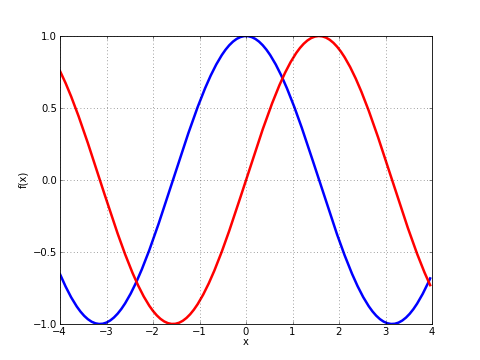
\includegraphics[scale=1.0]{Charts/png/MpMathPlot.png}
	\caption{MpMath 2Dplot}
	\label{Fig MpMath 2Dplot}
\end{figure}


Output of plot([cos, sin], [-4, 4])

\vpara
mpmath.plot(ctx, f, xlim=[-5, 5], ylim=None, points=200, file=None, dpi=None, singularities=[], axes=None)

\vpara
Shows a simple 2D plot of a function $f(x)$ or list of functions $[f_0(x),f_1(x),\ldots,f_n(x)]$ over a given interval specified by xlim. Some examples:

\lstset{language={Python}}
\begin{lstlisting}
plot(lambda x: exp(x)*li(x), [1, 4])
plot([cos, sin], [-4, 4])
plot([fresnels, fresnelc], [-4, 4])
plot([sqrt, cbrt], [-4, 4])
plot(lambda t: zeta(0.5+t*j), [-20, 20])
plot([floor, ceil, abs, sign], [-5, 5])
\end{lstlisting}


Points where the function raises a numerical exception or returns an infinite value are removed from the graph. Singularities can also be excluded explicitly as follows (useful
for removing erroneous vertical lines):

\lstset{language={Python}}
\begin{lstlisting}
plot(cot, ylim=[-5, 5]) # bad
plot(cot, ylim=[-5, 5], singularities=[-pi, 0, pi]) # good
\end{lstlisting}


For parts where the function assumes complex values, the real part is plotted with dashes and the imaginary part is plotted with dots.

Note: This function requires matplotlib (pylab).

\newpage
\subsubsection{Complex function plots}

\begin{figure}[ht]
	\centering
	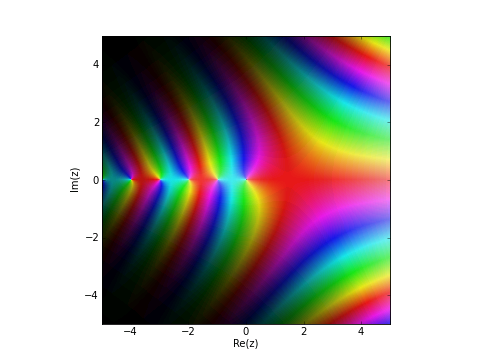
\includegraphics[scale=1.0]{Charts/png/MpMathCplot.png}
	\caption{MpMath cplot}
	\label{Fig MpMath cplot}
\end{figure}



Output of fp.cplot(fp.gamma, points=100000)

\vpara
mpmath.cplot(ctx, f, re=[-5, 5], im=[-5, 5], points=2000, color=None, verbose=False, file=None, dpi=None, axes=None)

\vpara
Plots the given complex-valued function f over a rectangular part of the complex plane specified by the pairs of intervals re and im. For example:

\lstset{language={Python}}
\begin{lstlisting}
cplot(lambda z: z, [-2, 2], [-10, 10])
cplot(exp)
cplot(zeta, [0, 1], [0, 50])
\end{lstlisting}


By default, the complex argument (phase) is shown as color (hue) and the magnitude is show as brightness. You can also supply a custom color function (color). This function should take a complex number as input and return an RGB 3-tuple containing floats in the range 0.0-1.0.

\vpara
To obtain a sharp image, the number of points may need to be increased to 100,000 or thereabout. Since evaluating the function that many times is likely to be slow, the 'verbose' option is useful to display progress.

Note: This function requires matplotlib (pylab).


\newpage
\subsubsection{3D surface plots}


Output of splot for the donut example.

\vpara
mpmath.splot(ctx, f, u=[-5, 5], v=[-5, 5], points=100, keep\_aspect=True, wireframe=False, file=None, dpi=None, axes=None)

\begin{figure}[ht]
	\centering
	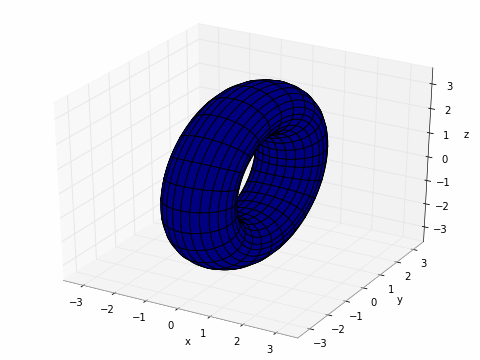
\includegraphics[scale=1.0]{Charts/png/MpMathSplot.png}
	\caption{MpMath Surface plot}
	\label{Fig MpMath Surface plot}
\end{figure}


Plots the surface defined by $f$.

\vpara
If $f$ returns a single component, then this plots the surface defined by $z=f(x,y)$ over the rectangular domain with $x=u$  and $y=v$.

\vpara
If $f$ returns three components, then this plots the parametric surface $x,y,z = f(u,v)$ over the pairs of intervals $u$ and $v$.

\vpara
For example, to plot a simple function:

\lstset{language={Python}}
\begin{lstlisting}
>>> from mpmath import *
>>> f = lambda x, y: sin(x+y)*cos(y)
>>> splot(f, [-pi,pi], [-pi,pi])
\end{lstlisting}


Plotting a donut:

\lstset{language={Python}}
\begin{lstlisting}
>>> r, R = 1, 2.5
>>> f = lambda u, v: [r*cos(u), (R+r*sin(u))*cos(v), (R+r*sin(u))*sin(v)]
>>> splot(f, [0, 2*pi], [0, 2*pi])
\end{lstlisting}


Note: This function requires matplotlib (pylab) 0.98.5.3 or higher.


\subsection{Using the C-API}

This section describes how to write modules in C or C++ to extend the Python interpreter with new modules. Those modules can not only define new functions but also new object types and their methods. The document also describes how to embed the Python interpreter in another application, for use as an extension language. Finally, it shows how to compile and link extension modules so that they can be loaded dynamically (at run time) into the interpreter, if the underlying operating system supports this feature.

This document assumes basic knowledge about Python. For an informal introduction to the language, see The Python Tutorial. The Python Language Reference gives a more formal definition of the language. The Python Standard Library documents the existing object types, functions and modules (both built-in and written in Python) that give the language its wide application range.

For a detailed description of the whole Python/C API, see the separate Python/C API Reference Manual.

. Extending Python with C or C++

It is quite easy to add new built-in modules to Python, if you know how to program in C. Such extension modules can do two things that can’t be done directly in Python: they can implement new built-in object types, and they can call C library functions and system calls.

To support extensions, the Python API (Application Programmers Interface) defines a set of functions, macros and variables that provide access to most aspects of the Python run-time system. The Python API is incorporated in a C source file by including the header "Python.h".

The compilation of an extension module depends on its intended use as well as on your system setup; details are given in later chapters.

Note:
The C extension interface is specific to CPython, and extension modules do not work on other Python implementations. In many cases, it is possible to avoid writing C extensions and preserve portability to other implementations. For example, if your use case is calling C library functions or system calls, you should consider using the ctypes module or the cffi library rather than writing custom C code. These modules let you write Python code to interface with C code and are more portable between implementations of Python than writing and compiling a C extension module.

As an example for an extension module which provides additional functionality in multi-precision computing, see the documentation on gmpy2 (section \ref{gmpy2}).





\subsection{Interfaces to the C family of languages}

\subsubsection{Windows, GNU/Linux, Mac OSX: GNU Compiler Collection}
The GNU Compiler Collection (GCC) is a compiler system produced by the GNU Project supporting various programming languages. GCC is a key component of the GNU toolchain. The Free Software Foundation (FSF) distributes GCC under the GNU General Public License (GNU GPL). GCC has played an important role in the growth of free software, as both a tool and an example.

\vpara
Originally named the GNU C Compiler, because it only handled the C programming language, GCC 1.0 was released in 1987 and the compiler was extended to compile C++ in December of that year.[1] Front ends were later developed for Objective-C, Objective-C++, Fortran, Java, Ada, and Go among others.[3]

\vpara
As well as being the official compiler of the unfinished GNU operating system, GCC has been adopted as the standard compiler by most other modern Unix-like computer operating systems, including Linux and the BSD family. A port to RISC OS has also been developed extensively in recent years. There is also an old (3.0) port of GCC to Plan9, running under its ANSI/POSIX Environment (APE).[4] GCC is also available for Microsoft Windows operating systems and for the ARM processor used by many portable devices.

\vpara
For further information on the GNU Compiler Collection, see \href{http://en.wikipedia.org/wiki/GNU_Compiler_Collection}{Wikipedia: GCC} (the text above has been copied from this reference), or the  \href{http://gcc.gnu.org/}{GCC Homepage}.


\subsubsection{Windows: MSVC}
Microsoft Visual C++ (often abbreviated as MSVC or VC++) is a commercial (free version available), integrated development environment (IDE) product from Microsoft for the C, C++, and C++/CLI programming languages. It features tools for developing and debugging C++ code, especially code written for the Microsoft Windows API, the DirectX API, and the Microsoft .NET Framework.

\vpara
Although the product originated as an IDE for the C programming language, the compiler's support for that language conforms only to the original edition of the C standard, dating from 1989. The later revisions of the standard, C99 and C11, are not supported.[41] According to Herb Sutter, the C compiler is only included for "historical reasons" and is not planned to be further developed. Users are advised to either use only the subset of the C language that is also valid C++, and then use the C++ compiler to compile their code, or to just use a different compiler such as Intel C++ Compiler or the GNU Compiler Collection instead.[42]

\vpara
For further information on Microsoft Visual C++, see \href{http://en.wikipedia.org/wiki/Visual_C\%2B\%2B}{Wikipedia: MSVC} (the text above has been copied from this reference), or the  \href{http://msdn.microsoft.com/en-us/vstudio/hh386302}{MSVC Homepage}.


\vpara
The following C file makes a number of direct calls into Python, passing arguments as strings and receiving a result as string:

\lstset{language={C++}}
\begin{lstlisting}

#include "stdafx.h"
#include "CallPython.h"

int main(int argc, const char *argv[])
{
long ResultLong = SetSpecialValue_Long(2,3,4);
printf( "This is a long: %d\n",  ResultLong);

double ResultDouble = SetSpecialValue_Double(2.0,3.0,4.0);
printf( "This is a double: %f\n",  ResultDouble);

const char *sLong2[] = {"TestLong", "lll", "3", "1432"};
MyPythonFunction(4, sLong2);

const char *sDouble2[] = {"TestDouble", "fff", "13.5", "265.34"};
MyPythonFunction(4, sDouble2);

const char *sString2[] = {"TestStringFunc", "sss", "3", "2"};
MyPythonFunction(4, sString2);

const char *sString3[] = {"TestStringMpf2", "3", "2.456"};
MyPythonFunctionString2(3, sString3);

char buffer[1600]; // 1600 bytes allocated here on the stack.
int size0a = MyPythonFunctionStringReturn(3, sString3, buffer, sizeof(buffer));
printf("New New0a %s\n", buffer); // prints "Mar"
//printf("Length of string: %ld\n", size0a);

char buffer0[1600]; // 1600 bytes allocated here on the stack.
int size0 = MyPythonFunctionStringReturn00("TestStringMpf0", buffer0, sizeof(buffer0));
printf("New New0 %s\n", buffer0); // prints "Mar"
//printf("Length of string0: %ld\n", size0);

char buffer1[1600]; // 1600 bytes allocated here on the stack.
int size1 = MyPythonFunctionStringReturn01("TestStringMpf1", "3", buffer1, sizeof(buffer1));
printf("New New1 %s\n", buffer1); // prints "Mar"
//printf("Length of string: %ld\n", size1);

char buffer2[1600]; // 1600 bytes allocated here on the stack.
int size2 = MyPythonFunctionStringReturn02("TestStringMpf2", "3", "2.456", buffer2, sizeof(buffer2));
printf("New New2 %s\n", buffer2); // prints "Mar"
//printf("Length of string: %ld\n", size2);

ClosePy();
return 0;
}

\end{lstlisting}

The header file CallPython.h looks like this:

\begin{lstlisting}
#pragma warning(disable: 4244)

#ifdef CALLPYTHON_EXPORTS
#define MPNUMC_DLL_IMPORTEXPORT __declspec(dllexport)
#else
#define MPNUMC_DLL_IMPORTEXPORT __declspec(dllimport)
#endif

#ifdef __cplusplus
extern "C" {
#endif

MPNUMC_DLL_IMPORTEXPORT long SetSpecialValue_Long(long m, long n, long what);
MPNUMC_DLL_IMPORTEXPORT double SetSpecialValue_Double(double m, double n, double what);
MPNUMC_DLL_IMPORTEXPORT int CallPythonFunction(int argc, const char *argv[]);
MPNUMC_DLL_IMPORTEXPORT int MyPythonFunction(int argc, const char *argv[]);
MPNUMC_DLL_IMPORTEXPORT int MyPythonFunctionString(int argc, const char *argv[]);
MPNUMC_DLL_IMPORTEXPORT int MyPythonFunctionString2(int argc, const char *argv[]);
MPNUMC_DLL_IMPORTEXPORT int MyPythonFunctionStringReturn(int argc, const char *argv[], char* buffer, int buffersize);

MPNUMC_DLL_IMPORTEXPORT int MyPythonFunctionStringReturn00(const char* FuncName, char* buffer, int buffersize);
MPNUMC_DLL_IMPORTEXPORT int MyPythonFunctionStringReturn01(const char* FuncName, const char* Arg01, char* buffer, int buffersize);
MPNUMC_DLL_IMPORTEXPORT int MyPythonFunctionStringReturn02(const char* FuncName, const char* Arg01, const char* Arg02, char* buffer, int buffersize);

MPNUMC_DLL_IMPORTEXPORT void ClosePy();
#ifdef __cplusplus
}
#endif
\end{lstlisting}


The C file CallPython.cpp (which produces the dynamic link library) looks like this:

\lstset{language={C++}}
\begin{lstlisting}

#define _CRT_SECURE_NO_WARNINGS
#include "CallPython.h"
#include "stdafx.h"
#include<stdio.h>
#include <Python.h>

long SetSpecialValue_Long(long m, long n, long what)
{
return (m + n + 1) * what;
}

double SetSpecialValue_Double(double m, double n, double what)
{
return (m + n) * what;
}


int MyPythonFunctionStringReturn00(const char* FuncName, char* buffer, int buffersize)
{
PyObject *pFunc;
PyObject *pValue;
Py_ssize_t size;
PyObject *pModule= GetPythonModule2();
pFunc = PyObject_GetAttrString(pModule, FuncName);
if (pFunc && PyCallable_Check(pFunc)) {
pValue = PyObject_CallObject(pFunc, NULL);
if (pValue != NULL) {
strncpy(buffer, PyUnicode_AsUTF8AndSize(pValue, &size), buffersize-1);
Py_DECREF(pValue);
}
}
Py_XDECREF(pFunc);
return size;
}


int MyPythonFunctionStringReturn01(const char* FuncName, const char* Arg01, char* buffer, int buffersize)
{
PyObject *pFunc, *pArgs, *pValue;
PyObject *pModule= GetPythonModule2();
Py_ssize_t size;
pFunc = PyObject_GetAttrString(pModule, FuncName);
if (pFunc && PyCallable_Check(pFunc)) {
pArgs = PyTuple_New(1);
pValue = PyUnicode_FromString(Arg01);
PyTuple_SetItem(pArgs, 0, pValue);

pValue = PyObject_CallObject(pFunc, pArgs);
Py_DECREF(pArgs);
if (pValue != NULL) {
strncpy(buffer, PyUnicode_AsUTF8AndSize(pValue, &size), buffersize-1);
Py_DECREF(pValue);
}
}
Py_XDECREF(pFunc);
return size;
}


int MyPythonFunctionStringReturn02(const char* FuncName, const char* Arg01, const char* Arg02, char* buffer, int buffersize)
{
PyObject *pFunc, *pArgs, *pValue;
PyObject *pModule= GetPythonModule2();
Py_ssize_t size;

pFunc = PyObject_GetAttrString(pModule, FuncName);

if (pFunc && PyCallable_Check(pFunc)) {
pArgs = PyTuple_New(2);
pValue = PyUnicode_FromString(Arg01);
PyTuple_SetItem(pArgs, 0, pValue);

pValue = PyUnicode_FromString(Arg02);
PyTuple_SetItem(pArgs, 1, pValue);

pValue = PyObject_CallObject(pFunc, pArgs);
Py_DECREF(pArgs);
if (pValue != NULL) {
strncpy(buffer, PyUnicode_AsUTF8AndSize(pValue, &size), buffersize-1);
Py_DECREF(pValue);
}
}
Py_XDECREF(pFunc);
return size;
}

void ClosePy()
{
PyObject *pModule;
pModule = GetPythonModule2();
Py_DECREF(pModule);
Py_Finalize();
}
\end{lstlisting}




\newpage
\subsection{Cython: C extensions for the Python language}

[Cython] is a programming language that makes writing C extensions for the Python language as easy as Python itself. It aims to become a superset of the [Python] language which gives it high-level, object-oriented, functional, and dynamic programming. Its main feature on top of these is support for optional static type declarations as part of the language. The source code gets translated into optimized C/C++ code and compiled as Python extension modules. This allows for both very fast program execution and tight integration with external C libraries, while keeping up the high programmer productivity for which the Python language is well known.

The primary Python execution environment is commonly referred to as CPython, as it is written in C. Other major implementations use Java (Jython [Jython]), C\# (IronPython [IronPython]) and Python itself (PyPy [PyPy]). Written in C, CPython has been conducive to wrapping many external libraries that interface through the C language. It has, however, remained non trivial to write the necessary glue code in C, especially for programmers who are more fluent in a high-level language like Python than in a close-to-the-metal language like C.

Originally based on the well-known Pyrex [Pyrex], the Cython project has approached this problem by means of a source code compiler that translates Python code to equivalent C code. This code is executed within the CPython runtime environment, but at the speed of compiled C and with the ability to call directly into C libraries. At the same time, it keeps the original interface of the Python source code, which makes it directly usable from Python code. These two-fold characteristics enable Cython’s two major use cases: extending the CPython interpreter with fast binary modules, and interfacing Python code with external C libraries.

While Cython can compile (most) regular Python code, the generated C code usually gains major (and sometime impressive) speed improvements from optional static type declarations for both Python and C types. These allow Cython to assign C semantics to parts of the code, and to translate them into very efficient C code. Type declarations can therefore be used for two purposes: for moving code sections from dynamic Python semantics into static-and-fast C semantics, but also for directly manipulating types defined in external libraries. Cython thus merges the two worlds into a very broadly applicable programming language.



\subsection{A Windows-specific interface: using COM}
\vpara
Example for using the library

\lstset{language={Python}}
\begin{lstlisting}
#Enable COM support
from win32com.client import Dispatch

#Load the mpNumerics library
mp = Dispatch("mpNumerics.mp_Lib")

#Set Floating point type to MPFR with 60 decimal digits precision
mp.FloatingPointType = 3
mp.Prec10 = 60

#Assign values to x1 and x2
x1 = mp.Real(4.5)
x2 = mp.Real(1.21)

#Calculate x3 = x1 / x2
x3 = x1.Div(x2)

#Print the value of x3
print (x3.Str())
\end{lstlisting}

\vpara
Example for using Excel

\lstset{language={Python}}
\begin{lstlisting}
#Enable COM support
from win32com.client import Dispatch

#Load the Excel library
xl = Dispatch("Excel.Application")
xl.Visible = 1
xl.Workbooks.Add() 
xl.Cells(1,1).Value = "Hello442" 
print("From Python")
\end{lstlisting}




\newpage
\section{R (Statistical System)}

R is a free software programming language and a software environment for statistical computing and graphics. The R language is widely used among statisticians and data miners for developing statistical software[2][3] and data analysis.[3] Polls and surveys of data miners are showing R's popularity has increased substantially in recent years.[4][5][6]

\vpara
R is an implementation of the S programming language combined with lexical scoping semantics inspired by Scheme. S was created by John Chambers while at Bell Labs. R was created by Ross Ihaka and Robert Gentleman[7] at the University of Auckland, New Zealand, and is currently developed by the R Development Core Team, of which Chambers is a member. R is named partly after the first names of the first two R authors and partly as a play on the name of S.[8]

\vpara
R is a GNU project.[9][10] The source code for the R software environment is written primarily in C, Fortran, and R.[11] R is freely available under the GNU General Public License, and pre-compiled binary versions are provided for various operating systems. R uses a command line interface; however, several graphical user interfaces are available for use with R.

\vpara
R provides a wide variety of statistical and graphical techniques, including linear and nonlinear modeling, classical statistical tests, time-series analysis, classification, clustering, and others. R is easily extensible through functions and extensions, and the R community is noted for its active contributions in terms of packages. There are some important differences, but much code written for S runs unaltered. Many of R's standard functions are written in R itself, which makes it easy for users to follow the algorithmic choices made. For computationally intensive tasks, C, C++, and Fortran code can be linked and called at run time. Advanced users can write C, C++[12] or Java[13] code to manipulate R objects directly.

\vpara
R is highly extensible through the use of user-submitted packages for specific functions or specific areas of study. Due to its S heritage, R has stronger object-oriented programming facilities than most statistical computing languages. Extending R is also eased by its lexical scoping rules.[14]

\vpara
Another strength of R is static graphics, which can produce publication-quality graphs, including mathematical symbols. Dynamic and interactive graphics are available through additional packages.[15]

\vpara
R has its own LaTeX-like documentation format, which is used to supply comprehensive documentation, both on-line in a number of formats and in hard copy.

\vpara
R is an interpreted language; users typically access it through a command-line interpreter. If a user types "2+2" at the R command prompt and presses enter, the computer replies with "4", as shown below:

> 2+2

[1] 4

\vpara
Like many other languages, R supports matrix arithmetic. R's data structures include scalars, vectors, matrices, data frames (similar to tables in a relational database) and lists.[16] R's extensible object-system includes objects for (among others): regression models, time-series and geo-spatial coordinates.

\vpara
R supports procedural programming with functions and, for some functions, object-oriented programming with generic functions. A generic function acts differently depending on the type of arguments passed to it. In other words, the generic function dispatches the function (method) specific to that type of object. For example, R has a generic print() function that can print almost every type of object in R with a simple "print(objectname)" syntax.

\vpara
Although mostly used by statisticians and other practitioners requiring an environment for statistical computation and software development, R can also operate as a general matrix calculation toolbox - with performance benchmarks comparable to GNU Octave or MATLAB.[17]

\vpara
For further information on R, see \href{http://en.wikipedia.org/wiki/R_(programming_language)}{Wikipedia: R} (the text above has been copied from this reference), or the  \href{http://www.r-project.org/}{R Homepage}.

%\vpara
%COM support can be obtained by installing the \href{http://www.omegahat.org/RDCOMClient/}{R RDCOMClient} 
%
%Installation of the binary should be as straightforward as any other R package for Windows, e.g. use the command 
%
%\begin{verbatim} 
%install.packages("RDCOMClient", repos = "http://www.omegahat.org/R")
%\end{verbatim}
%
%or use the Packages menu and make certain to include the Omegahat repository in the list of repositories to search. 
%
%There exists also a commercial \href{http://rcom.univie.ac.at/main.html}{R for Excel distribution}.

\vpara
A popular GUI for R is \href{http://www.rstudio.com/}{Rstudio}.

Within RStudio:

Tools - Install Packages.

Type RD in the dialogue box.

RDCOMClient should appear in the drop down box.

Select RDCOMClient and click on Install.

Needs to be done separately for 32 bit and 64 bit.

\vpara
R contains packages which provide interfaces to 

GMP (\href{http://mulcyber.toulouse.inra.fr/projects/gmp}{http://mulcyber.toulouse.inra.fr/projects/gmp}) and 

MPFR (\href{http://rmpfr.r-forge.r-project.org/}{http://rmpfr.r-forge.r-project.org/}). 

\vpara
Book recommendation: \cite{Adler2012}.

Book recommendation: \cite{Verzani2011}.

Book recommendation: \cite{Chang2012}.

\vpara
Example for using the library

\lstset{language={R}}
\begin{lstlisting}
#Enable COM support
require("RDCOMClient")

#Load the mpNumerics library
mp = COMCreate("mpNumerics.mp_Lib")

#Set Floating point type to MPFR with 60 decimal digits precision
mp[["Prec10"]] = 160
mp[["FloatingPointType"]] = 3

#Assign values to x1 and x2
x1 = mp$Real("4.5")
x2 = mp$Real("1.1")

#Perform arithmetic operations
x3 = x1$Plus(x2)
x4 = x1$Div(x2)

#Display output
mp[["Prec10"]]
x3$Str()
x4$Str()
\end{lstlisting}

\vpara
Example for using Excel

\lstset{language={R}}
\begin{lstlisting}
#Load Library
require("rcom")

#Create instance of Excel
xlApp = comCreateObject("Excel.Application")

#Add 1 workbook and make it visible
wb = xlApp[["Workbooks"]]$Add()
xlApp[["Visible"]] = TRUE

#Display the name of the 1st worksheet
ws = wb[["Worksheets", 1]]
wsname = ws[["Name"]]
wsname

#Assign values to a range
mrange = ws[["Range", "A1:B10"]]
mrange[["Value"]] = 10.3

#Display the values of the range
d = mrange[["Value"]]
d
$
\end{lstlisting}

Within RStudio, on the menu bar, click Tools -> Install packages.

In the textbox "Packages" enter "RMpfr" and click on "Install".

This should install the RMpfr and GMP packages.

\lstset{language={R}}
\begin{lstlisting}
#Load Library
require("Rmpfr")

n1.25 <- mpfr(5, precBits = 256)/4
n1.25

n1.25 ^ c(1:7, 20, 30)

exp(n1.25)

getGroupMembers("Math")

showMethods(classes = "mpfr")

showMethods(classes = "mpfrArray")

\end{lstlisting}





\chapter{Acknowledgements} 

\section{Contributors to libraries used in the numerical routines}

\subsection{Contributors to GMP}
\label{Contributors to GMP}
The following text has been copied from the GMP manual (5.1.2):

\vpara
"Torbj\"orn Granlund wrote the original GMP library and is still the main
developer.  Code not explicitly attributed to others, was contributed by
Torbj\"orn.  Several other individuals and organizations have contributed
GMP.  Here is a list in chronological order on first contribution:

\vpara
Gunnar Sj\"odin and Hans Riesel helped with mathematical problems in early
versions of the library.

\vpara
Richard Stallman helped with the interface design and revised the first
version of this manual.

\vpara
Brian Beuning and Doug Lea helped with testing of early versions of the
library and made creative suggestions.

\vpara
John Amanatides of York University in Canada contributed the function
$\mathtt{mpz\_probab\_prime\_p}$.

\vpara
Paul Zimmermann wrote the REDC-based mpz\_powm code, the Sch\"onhage-Strassen
FFT multiply code, and the Karatsuba square root code.  He also improved the
Toom3 code for GMP 4.2.  Paul sparked the development of GMP 2, with his
comparisons between bignum packages.  The ECMNET project Paul is organizing
was a driving force behind many of the optimizations in GMP 3.  Paul also
wrote the new GMP 4.3 nth root code (with Torbj\"orn).

\vpara
Ken Weber (Kent State University, Universidade Federal do Rio Grande do Sul)
contributed now defunct versions of $\mathtt{mpz\_gcd}$, $\mathtt{mpz\_divexact}$,
$\mathtt{mpn\_gcd}$, and $\mathtt{mpn\_bdivmod}$, partially supported by CNPq (Brazil)
grant 301314194-2.

\vpara
Per Bothner of Cygnus Support helped to set up GMP to use Cygnus' configure.
He has also made valuable suggestions and tested numerous intermediary
releases.

\vpara
Joachim Hollman was involved in the design of the $\mathtt{mpf}$ interface, and in
the $\mathtt{mpz}$ design revisions for version 2.

\vpara
Bennet Yee contributed the initial versions of $\mathtt{mpz\_jacobi}$ and
$\mathtt{mpz\_legendre}$.

\vpara
Andreas Schwab contributed the files $\mathtt{mpn/m68k/lshift.S}$ and
$\mathtt{mpn/m68k/rshift.S}$ (now in $\mathtt{.asm}$ form).

\vpara
Robert Harley of Inria, France and David Seal of ARM, England, suggested clever
improvements for population count.  Robert also wrote highly optimized
Karatsuba and 3-way Toom multiplication functions for GMP 3, and contributed
the ARM assembly code.

\vpara
Torsten Ekedahl of the Mathematical department of Stockholm University provided
significant inspiration during several phases of the GMP development.  His
mathematical expertise helped improve several algorithms.

\vpara
Linus Nordberg wrote the new configure system based on autoconf and
implemented the new random functions.

\vpara
Kevin Ryde worked on a large number of things: optimized x86 code, m4 asm
macros, parameter tuning, speed measuring, the configure system, function
inlining, divisibility tests, bit scanning, Jacobi symbols, Fibonacci and Lucas
number functions, printf and scanf functions, perl interface, demo expression
parser, the algorithms chapter in the manual, $\mathtt{gmpasm-mode.el}$, and
various miscellaneous improvements elsewhere.

\vpara
Kent Boortz made the Mac OS 9 port.

\vpara
Steve Root helped write the optimized alpha 21264 assembly code.

\vpara
Gerardo Ballabio wrote the $\mathtt{gmpxx.h}$ C++ class interface and the C++
$\mathtt{istream}$ input routines.

\vpara
Jason Moxham rewrote $\mathtt{mpz\_fac\_ui}$.

\vpara
Pedro Gimeno implemented the Mersenne Twister and made other random number
improvements.

\vpara
Niels M\"oller wrote the sub-quadratic GCD, extended GCD and jacobi code, the
quadratic Hensel division code, and (with Torbj\"orn) the new divide and
conquer division code for GMP 4.3.  Niels also helped implement the new Toom
multiply code for GMP 4.3 and implemented helper functions to simplify Toom
evaluations for GMP 5.0.  He wrote the original version of $\mathtt{mpn\_mulmod\_bnm1}$, and
he is the main author of the mini-gmp package used for gmp bootstrapping.

\vpara
Alberto Zanoni and Marco Bodrato suggested the unbalanced multiply strategy,
and found the optimal strategies for evaluation and interpolation in Toom
multiplication.

\vpara
Marco Bodrato helped implement the new Toom multiply code for GMP 4.3 and
implemented most of the new Toom multiply and squaring code for 5.0.
He is the main author of the current mpn\_mulmod\_bnm1 and mpn\_mullo\_n.  Marco
also wrote the functions mpn\_invert and mpn\_invertappr.  He is the author of
the current combinatorial functions: binomial, factorial, multifactorial,
primorial.

\vpara
David Harvey suggested the internal function $\mathtt{mpn\_bdiv\_dbm1}$, implementing
division relevant to Toom multiplication.  He also worked on fast assembly
sequences, in particular on a fast AMD64 $\mathtt{mpn\_mul\_basecase}$. He wrote
the internal middle product functions $\mathtt{mpn\_mulmid\_basecase}$, \\
$\mathtt{mpn\_toom42\_mulmid}$, $\mathtt{mpn\_mulmid\_n}$ and related helper routines.

\vpara
Martin Boij wrote $\mathtt{mpn\_perfect\_power\_p}$.

\vpara
Marc Glisse improved $\mathtt{gmpxx.h}$: use fewer temporaries (faster),
specializations of $\mathtt{numeric\_limits}$ and $\mathtt{common\_type}$, C++11
features (move constructors, explicit bool conversion, UDL), make the
conversion from $\mathtt{mpq\_class}$ to $\mathtt{mpz\_class}$ explicit, optimize
operations where one argument is a small compile-time constant, replace
some heap allocations by stack allocations.  He also fixed the eofbit
handling of C++ streams, and removed one division from $\mathtt{mpq/aors.c}$.

\vpara
(This list is chronological, not ordered after significance.  If you have
contributed to GMP but are not listed above, please tell
$\mathtt{gmp-devel@gmplib.org}$ about the omission!)

\vpara
The development of floating point functions of GNU MP 2, were supported in part
by the ESPRIT-BRA (Basic Research Activities) 6846 project POSSO (POlynomial
System SOlving).

\vpara
The development of GMP 2, 3, and 4 was supported in part by the IDA Center for
Computing Sciences.

\vpara
Thanks go to Hans Thorsen for donating an SGI system for the GMP test system
environment."





\subsection{Contributors to MPFR}
\label{Contributors to MPFR}
The following text has been copied from the MPFR manual (3.1.2):

\vpara
"The main developers of MPFR are Guillaume Hanrot, Vincent Lef\`evre,
Patrick P\'elissier, Philippe Th\'eveny and Paul Zimmermann.

\vpara
Sylvie Boldo from ENS-Lyon, France,
contributed the functions $\mathtt{mpfr\_agm}$ and $\mathtt{mpfr\_log}$.
Sylvain Chevillard contributed the $\mathtt{mpfr\_ai}$ function.

\vpara
David Daney contributed the hyperbolic and inverse hyperbolic functions,
the base-2 exponential, and the factorial function.

\vpara
Alain Delplanque contributed the new version of the $\mathtt{mpfr\_get\_str}$
function.

\vpara
Mathieu Dutour contributed the functions $\mathtt{mpfr\_acos}$, $\mathtt{mpfr\_asin}$
and $\mathtt{mpfr\_atan}$, and a previous version of $\mathtt{mpfr\_gamma}$.

\vpara
Laurent Fousse contributed the $\mathtt{mpfr\_sum}$ function.

\vpara
Emmanuel Jeandel, from ENS-Lyon too,
contributed the generic hypergeometric code,
as well as the internal function $\mathtt{mpfr\_exp3}$,
a first implementation of the sine and cosine,
and improved versions of
$\mathtt{mpfr\_const\_log2}$ and $\mathtt{mpfr\_const\_pi}$.

\vpara
Ludovic Meunier helped in the design of the $\mathtt{mpfr\_erf}$ code.

\vpara
Jean-Luc R\'emy contributed the $\mathtt{mpfr\_zeta}$ code.

\vpara
Fabrice Rouillier contributed the $\mathtt{mpfr\_xxx\_z}$ and $\mathtt{mpfr\_xxx\_q}$
functions, and helped to the Microsoft Windows porting.

\vpara
Damien Stehl\'e contributed the $\mathtt{mpfr\_get\_ld\_2exp}$ function.

\vpara
We would like to thank Jean-Michel Muller and Joris van der Hoeven for very
fruitful discussions at the beginning of that project, Torbj\"orn Granlund
and Kevin Ryde for their help about design issues,
and Nathalie Revol for her careful reading of a previous version of
this documentation. In particular
Kevin Ryde did a tremendous job for the portability of MPFR in 2002-2004.

\vpara
The development of the MPFR library would not have been possible without
the continuous support of INRIA, and of the LORIA (Nancy, France) and LIP
(Lyon, France) laboratories. In particular the main authors were or are
members of the PolKA, Spaces, Cacao and Caramel
project-teams at LORIA and of the
Ar\'enaire and AriC project-teams at LIP.

This project was started during the Fiable (reliable in French) action
supported by INRIA, and continued during the AOC action.
The development of MPFR was also supported by a grant
(202F0659 00 MPN 121) from the Conseil R\'egional de Lorraine in 2002,
from INRIA by an "associate engineer" grant (2003-2005),
an "op\'eration de d\'eveloppement logiciel" grant (2007-2009),
and the post-doctoral grant of Sylvain Chevillard in 2009-2010.
The MPFR-MPC workshop in June 2012 was partly supported by the ERC
grant ANTICS of Andreas Enge."


%
%
%\subsection{Contributors to MPC}
%\label{Contributors to MPC}
%The main developers of MPC are Andreas Enge, Philippe Th\'eveny and Paul Zimmermann.
%
%
%
%\subsection{Contributors to MPFI}
%\label{Contributors to MPFI}
%The following text has been copied from the MPFI manual (1.5.1):
%
%\vpara
%"MPFI has been written by Fabrice Rouillier, Nathalie Revol, Sylvain Chevillard, Hong Diep
%Nguyen, Christoph Lauter and Philippe Th\'eveny. Its development has greatly benefited from
%the patient and supportive help of the MPFR team."
%


%\section{Contributors to libraries used in the numerical routines}

\subsection{Contributors to FLINT}
\label{Contributors to FLINT}
The following text has been copied from the FLINT manual (2.4.3):

\vpara
xxxx


\subsection{Contributors to ARB}
\label{Contributors to ARB}
The following text has been copied from the FLINT manual (2.4.3):

\vpara
xxxx

%
%
%\subsection{Contributors to mpMath}
%\label{Contributors to mpMath}
%The following text has been copied from the mpMath manual (0.19):
%
%\vpara
%xxxx
%

%
%
%\subsection{Contributors to XSC}
%\label{Contributors to XSC}
%The main developers of XSC are Frithjof Blomquist, Werner Hofschuster, Walter Kr\"amer.
%
%\vpara
%The Credits sction from the C-XSC - A C++ Class Library for Extended Scientific Computing Documentation 2.5.3 main page http://www2.math.uni-wuppertal.de/~xsc/xsc/cxsc/apidoc/html/main.html contains the following statement:
%
%\vpara
%"The work on C-XSC started in 1990 at the Institute for Applied Mathematics (Prof. Kulisch), University of Karlsruhe. Many colleagues and scientists have directly and indirectly contributed to the realization of C-XSC. The authors would like to thank each of them for his or her cooperation. Special thanks go to U. Allendörfer, C. Baumhof, H. Berlejung, H. Bleher, H. Böhm, B. Bohl, G. Bohlender, F. Blomquist, K. Braune, H.H. Chen, D. Cordes, A. Davidenkoff, H.-C. Fischer, M. Grimmer, K. Grüner, R. Hammer, M. Hinz, M. Hocks, B. Höffgen, W. Hofschuster, P. Januscke, E. Kaucher, R. Kelch, R. Kirchner, R. Klatte, W. Klein, W. Krämer, U. Kulisch, C. Lawo, M. Metzger, W.L. Miranker, M. Neaga, M. Neher, D. Ratz, M. Rauch, S. Ritterbusch, S.M. Rump, R. Saier, D. Schiriaev, L. Schmidt, G. Schumacher, U. Storck, J. Suckfüll, F. Toussaint, C. Ullrich, W. Walter, S. Wedner, G. Werheit, A. Wiethoff, H.W. Wippermann, J. Wolff von Gudenberg and M. Zimmer.
%
%\vpara
%C-XSC is an outcome of an ongoing collaboration of the Institute for Applied Mathematics (Prof. Kulisch), University of Karlsruhe and the Institute for Scientific Computing/Software Engineering (Prof. Krämer), University of Wuppertal. For the latest news and up to date software contact http://www.math.uni-wuppertal.de/~xsc/ .
%
%\vpara
%Thanks to the referees for valuable comments and suggestions."
%
%
%
%\subsection{Contributors to XSC-MPFI}
%\label{Contributors to XSC-MPFI}
%The main developers of XSC-MPFI are Frithjof Blomquist, Werner Hofschuster, Walter Kr\"amer. 
%The library is in part based on work by Hans-Stephan Brand.
%


\subsection{Contributors to MPFRC++}
\label{Contributors to MPFRC++}
The main developer of MPFRC++ is Pavel Holoborodko.

Contributors:
Dmitriy Gubanov, Konstantin Holoborodko, Brian Gladman, 
Helmut Jarausch, Fokko Beekhof, Ulrich Mutze, Heinz van Saanen, 
Pere Constans, Peter van Hoof, Gael Guennebaud, Tsai Chia Cheng, 
Alexei Zubanov, Jauhien Piatlicki, Victor Berger, John Westwood.


%
%\subsection{Contributors to gmpfrxx}
%\label{Contributors to gmpfrxx}
%The main developer of gmpfrxx is Jon Wilkening.
%


\subsection{Contributors to Eigen}
\label{Contributors to Eigen}

The following statement is copied from the Eigen Homepage:

\vpara
"The Eigen project was started by Beno\^{i}t Jacob  (founder) and Ga\"{e}l Guennebaud (guru). Many other people have since contributed their talents to help make Eigen successful. Here's an alphabetical list: (note to contributors: do add yourself!) 

\vpara
Philip Avery:  Fix bug and add functionality to AutoDiff module  

Abraham Bachrach:  Added functions for cwise min/max with a scalar  

Sebastien Barthelemy:  Fix EIGEN\_INITIALIZE\_MATRICES\_BY\_NAN  

Carlos Becker:  Wrote some of the pages of the tutorial  

David Benjamin:  Artwork: the owls  

Cyrille Berger:  Fix error in logic of installation script  

Armin Berres:  Lots of fixes (compilation warnings and errors)  

Jose Luis Blanco:  Build fixes for MSVC and AMD64, correction in docs  

Mark Borgerding:  FFT module  

Romain Bossart:  Updates to Sparse solvers  

Kolja Brix:  Added documentation to Householder module, fixes for ARPACK wrapper and KroneckerProduct  

Gauthier Brun:  Making a start with a divide-and-conquer SVD implementation  

Thomas Capricelli:  Migration to mercurial, Non-linear optimization and numerical differentiation, cron-job to update the online dox 

Nicolas Carre:  Making a start with a divide-and-conquer SVD implementation  

Jean Ceccato:  Making a start with a divide-and-conquer SVD implementation  

Andrew Coles:  Fixes (including a compilation error)r  

Marton Danoczy:  MSVC compilation fix, support for ARM NEON with Clang 3.0 and LLVM-GCC  

Jeff Dean:  Fix in vectorized square root for small arguments  

Christian Ehrlicher:  MSVC compilation fix  

Daniel Gomez Ferro:  Improvements in Sparse and in matrix product  

Rohit Garg:  Vectorized quaternion and cross products, improved integer product  

Mathieu Gautier:  QuaternionMap and related improvements  

Anton Gladky:  Visual Studio 2008 and GCC 4.6 compilation fixes  

Stuart Glaser:  Prevent allocations in LU decomposition  

Marc Glisse:  C++11 compilation issues (suffices for literals)  

Frederic Gosselin:  Improve filter for hidden files in CMake  

Gaël Guennebaud:  Core developer  

Philippe Hamelin:  Allow CMake project to be included in another project  

Marcus D. Hanwell:  CMake improvements. Marcus is a developer at Kitware!  

David Harmon:  Arpack support module  

Chen-Pang He:  Many improvements to MatrixFunctions and KroneckerProduct modules  

Hauke Heibel:  Extended matrix functions, STL compatibility, Splines, CMake improvements, and more ...  

Christoph Hertzberg:  Quaternions, shifts for Cholmod, bug fixes, lots of user support on forums and IRC  

Pavel Holoborodko:  Multi-precision support with MPFR C++  

Tim Holy:  Improvements to tutorial, LDLT update and downdate  

Intel:  Back-end to Intel Math Kernel Library (MKL)  

Trevor Irons:  Square root for complex numbers, fix compile errors and mistake in docs  

Benoît Jacob : Core developer  

Bram de Jong:  Improvement to benchmark suite  

Kibeom Kim:  Implement *= /= * / operations for VectorwiseOp  

Claas Köhler:  Improvements to Fortran and FFTW in CMake  

Alexey Korepanov:  Add RealQZ class  

Igor Krivenko:  Properly cast constants when using non-standard scalars  

Marijn Kruisselbrink:  CMake fixes  

Moritz Lenz:  Allow solving transposed problem with SuperLU  

Sebastian Lipponer:  MSVC compilation support  

Daniel Lowenberg:  Add SparseView class  

David J. Luitz:  Bug fix for sparse * dense matrix product  

Angelos Mantzaflaris:  Fix to allow IncompleteLUT to be used with MPFR  

D J Marcin:  Fix operator \& precedence bug  

Konstantinos A. Margaritis:  AltiVec and ARM NEON vectorization  

Ricard Marxer:  Reverse, redux improvements, the count() method, some dox  

Vincenzo Di Massa:  CMake fix  

Christian Mayer:  Early code review and input in technical/design discussions  

Frank Meier-Dörnberg:  MSVC compatibility fixes  

Keir Mierle:  LDLT decomposition and other improvements, help with MPL relicensing  

Laurent Montel:  CMake improvements. Laurent is (with Alexander) one of the CMake gurus at KDE!  

Eamon Nerbonne:  Compilation fixes for win32  

Alexander Neundorf:  CMake improvements. Alexander is (with Laurent) one of the CMake gurus at KDE!  

Jason Newton:  Componentwise tangent functions  

Jitse Niesen:  Matrix functions, large improvements in the Eigenvalues module and in the docs, and more ...  

Desire Nuentsa:  Many improvements to Sparse module: SparseLU, SparseQR, ILUT, PaStiXSupport, …  

Jan Oberländer:  Compatibility with termios.h  

Jos van den Oever:  Compilation fix  

Michael Olbrich:  Early patches, including the initial loop meta-unroller  

Simon Pilgrim:  Optimizations for NEON  

Bjorn Piltz:  Visual C compilation fix  

Benjamin Piwowarski:  Add conservativeResize() for sparse matrices  

Zach Ploskey:  Copy-editing of tutorial  

Giacomo Po:  MINRES iterative solver  

Sergey Popov:  Fix bug in SelfAdjointEigenSolver  

Manoj Rajagopalan:  Introduce middleRows() / middleCols(), bug fix for nonstandard numeric types  

Stjepan Rajko:  MSVC compatibility fix  

Jure Repinc:  CMake fixes  

Kenneth Frank Riddile:  Lots of Windows/MSVC compatibility fixes, handling of alignment issues  

Adolfo Rodriguez:  Prevent allocations in matrix decompositions  

Peter Román : Support for SuperLU's ILU factorization  

Oliver Ruepp:  Bug fix in sparse matrix product with row-major matrices  

Radu Bogdan Rusu:  Fix compilation warning  

Guillaume Saupin:  Skyline matrices  

Michael Schmidt:  Fix in assembly when identifying CPU  

Jakob Schwendner:  Test for unaligned quaternions  

Martin Senst:  Bug fix for empty matrices  

Benjamin Schindler:  gdb pretty printers  

Michael Schmidt:  Compilation fix connected to min/max  

Dennis Schridde:  New typedefs like AlignedBox3f  

Jakob Schwendner:  Benchmark for Geometry module  

Sameer Sheorey:  Fix gdb pretty printer for variable-size matrices  

Andy Somerville:  Functions to get intersection between two ParametrizedLines  

Alex Stapleton:  Help with tough C++ questions  

Adam Szalkowski:  Bug fix in MatrixBase::makeHouseholder()  

Adolfo Rodriguez: Tsourouksdissian  Version of JacobiSVD that pre-allocates its resources  

Piotr Trojanek:  QCC compilation fixes  

Anthony Truchet:  Bugfix in QTransform and QMatrix support  

James Richard Tyrer:  CMake fix  

Rhys Ulerich:  Pkg-config support, improved GDB pretty-printer  

Ingmar Vanhassel:  CMake fix  

Scott Wheeler:  Documentation improvements  

Urs Wolfer:  Fixed a serious warning  

Manuel Yguel:  Bug fixes, work on inverse-with-check, the Polynomial module  

Pierre Zoppitelli:  Making a start with a divide-and-conquer SVD implementation  

\vpara
Eigen is also using code that we copied from other sources. They are acknowledged in our sources and in the Mercurial history, but let's also mention them here: 

\vpara
Intel Corporation  SSE code for 4x4 matrix inversion taken from here.  
Tim Davis  AMD reordering simplicial sparse Cholesky factorization adapted from SuiteSparse  
Julien Pommier  SSE implementation of exp,log,cos,sin math functions from GMM++  
Yousef Saad  IncompleteLUT preconditioner coming from ITSOL  
Minpack authors  Algorithms for non linear optimization.  

\vpara
Special thanks to Tuxfamily for the wonderful quality of their services, and the GCC Compile Farm Project that gives us access to many various systems including ARM NEON. "


%
%
%\subsection{Contributors to Amath}
%\label{Contributors to Amath}
%The main developer of Amath is Wolfgang Ehrhardt.
%



\subsection{Contributors to Boost Multiprecision}
\label{Contributors to Boost Multiprecision}
The main authors of Boost Multiprecision are John Maddock and Christopher Kormanyos.

\vpara
The Acknowledgements section states:

\vpara
"This library would not have happened without:

Christopher Kormanyos' C++ decimal number code.

Paul Bristow for patiently testing, and commenting on the library.

All the folks at GMP, MPFR and libtommath, for providing the "guts" that makes this library work.

"The Art Of Computer Programming", Donald E. Knuth, Volume 2: Seminumerical Algorithms, Third Edition (Reading, Massachusetts: Addison-Wesley, 1997), xiv+762pp. \\
ISBN 0-201-89684-2"



\subsection{Contributors to Boost Math}
\label{Contributors to Boost Math}
The main authors of the Boost Math Toolkit are Paul A. Bristow, Hubert Holin, Christopher Kormanyos, Bruno Lalande, John Maddock, Johan Råde, Benjamin Sobotta, Gautam
Sewani, Thijs van den Berg, Daryle Walker, and Xiaogang Zhang.

\vpara
The Credits and Acknowledgements section states:

\vpara
"Hubert Holin started the Boost.Math library. The Quaternions, Octonions, inverse hyperbolic functions, and the sinus cardinal functions are his.

\vpara
Daryle Walker wrote the integer gcd and lcm functions.

\vpara
John Maddock started the special functions, the beta, gamma, erf, polynomial, and factorial functions are his, as is the "Toolkit" section, and many of the statistical distributions.

\vpara
Paul A. Bristow threw down the challenge in A Proposal to add Mathematical Functions for Statistics to the C++ Standard Library to add the key math functions, especially those essential for statistics. After JM accepted and solved the diffi cult problems, not only numerically, but in full C++ template style, PAB implemented a few of the statistical distributions. PAB also tirelessly proof-read everything that JM threw at him (so that all remaining editorial mistakes are his fault).

\vpara
Xiaogang Zhang worked on the Bessel functions and elliptic integrals for his Google Summer of Code project 2006.

\vpara
Bruno Lalande submitted the "compile time power of a runtime base" code.

\vpara
Johan Råde wrote the optimised floating-point classifi cation and manipulation code, and nonfi nite f acets to permit C99 output of infinities and NaNs. (nonfi nite facets were not added until Boost 1.47 but had been in use with Boost.Spirit). This library was based on a suggestion from Robert Ramey, author of Boost.Serialization. Paul A. Bristow expressed the need for better handling of Input \& Output of NaN and infi nity for the C++ Standard Library  and suggested following the C99 format.

\vpara
Antony Polukhin improved lexical cast avoiding stringstream so that it was no longer necessary to use a globale C99 facet to handle nonfinites.

\vpara
Håkan Ardö, Boris Gubenko, John Maddock, Markus Schöpfl in and Olivier Verdier tested the floating-point library and Martin Bonner, Peter Dimov and John Maddock provided valuable advice.

\vpara
Gautam Sewani coded the logistic distribution as part of a Google Summer of Code project 2008.

\vpara
M. A. (Thijs) van den Berg coded the Laplace distribution. (Thijs has also threatened to implement some multivariate distributions).

\vpara
Thomas Mang requested the inverse gamma in chi squared distributions for Bayesian applications and helped in their implementation, and provided a nice example of their use.

\vpara
Professor Nico Temme for advice on the inverse incomplete beta function.

\vpara
Victor Shoup for NTL, without which it would have much more diffi cult to produce high accurac y constants, and especially the tables of accurate values for testing.

\vpara
We are grateful to Joel Guzman for helping us stress-test his Boost.Quickbook program used to generate the html and pdf versions of this document, adding several new features en route.

\vpara
Plots of the functions and distributions were prepared in W3C standard Scalable Vector Graphic (SVG) format using a program created by Jacob Voytko during a Google Summer of Code (2007). From 2012, the latest versions of all Internet Browsers have support for rendering SVG (with varying quality). Older versions, especially (Microsoft Internet Explorer (before IE 9) lack native SVG support but can be made to work with Adobe's free SVG viewer plugin). The SVG fi les can be con verted to JPEG or PNG using Inkscape.

\vpara
We are also indebted to Matthias Schabel for managing the formal Boost-review of this library, and to all the reviewers - including Guillaume Melquiond, Arnaldur Gylfason, John Phillips, Stephan Tolksdorf and Jeff Garland - for their many helpful comments.

\vpara
Thanks to Mark Coleman and Georgi Boshnakov for spot test values from Wolfram Mathematica, and of course, to Eric Weisstein for nurturing Wolfram MathWorld, an invaluable resource.

\vpara
The Skew-normal distribution and Owen's t function were written by Benjamin Sobotta."'




\subsection{Contributors to Boost Random}
\label{Contributors to Boost Random}
The main authors of the Boost Random are Jens Maurer and Steven Watanabe.

\vpara
The History and Acknowledgements section states:

\vpara
"In November 1999, Jeet Sukumaran proposed a framework based on virtual functions, and later sketched a template-based approach. Ed Brey pointed out that Microsoft Visual C++ does not support in-class member initializations and suggested the enum workaround. Dave Abrahams highlighted quantization issues. 

\vpara
The first public release of this random number library materialized in March 2000 after extensive discussions on the boost mailing list. Many thanks to Beman Dawes for his original min\_rand class, portability fixes, documentation suggestions, and general guidance. Harry Erwin sent a header file which provided additional insight into the requirements. Ed Brey and Beman Dawes wanted an iterator-like interface. 

\vpara
Beman Dawes managed the formal review, during which Matthias Troyer, Csaba Szepesvari, and Thomas Holenstein gave detailed comments. The reviewed version became an official part of boost on 17 June 2000. 

\vpara
Gary Powell contributed suggestions for code cleanliness. Dave Abrahams and Howard Hinnant suggested to move the basic generator templates from namespace boost::detail to boost::random. 

\vpara
Ed Brey asked to remove superfluous warnings and helped with uint64\_t handling. Andreas Scherer tested with MSVC. Matthias Troyer contributed a lagged Fibonacci generator. Michael Stevens found a bug in the copy semantics of normal\_distribution and suggested documentation improvements."







\subsection{Contributors to Boost Odeint}
\label{Contributors to Boost Odeint}
The main authors of the Boost Odeint are Karsten Ahnert  and Mario Mulansky.

\vpara
The History and Acknowledgements section states:

\vpara
Acknowledgments 

Steven Watanabe for managing the Boost review process. 

All people who participated in the odeint review process on the Boost mailing list. 

Paul Bristow for helping with the documentation. 

The Google Summer Of Code (GSOC) program for funding and Andrew Sutton for supervising us during the GSOC and for lots of useful discussions and feedback about many implementation details.. 

Joachim Faulhaber for motivating us to participate in the Boost review process and many detailed comments about the library. 

All users of odeint. They are the main motivation for our efforts. 

\vpara
 Contributers 

Andreas Angelopoulos implemented the sparse matrix implicit Euler stepper using the MTL4 library. 

Rajeev Singh implemented the stiff Van der Pol oscillator example. 

Sylwester Arabas improved the documentation. 

Denis Demidov provided the adaption to the VexCL and Viennacl libraries. 

Christoph Koke provided improved binders. 

Lee Hodgkinson provided the black hole example. 

Michael Morin fixed several typos in the documentation and the the source code comments. 

  





\subsection{Contributors to NLOpt}
\label{Contributors to NLOpt}
The main author of NLOpt is Steven G. Johnson.

\vpara
The Acknowledgements section states:

\vpara
"We are grateful to the many authors who have published useful optimization algorithms implemented in NLopt, especially those who have provided free/open-source implementations of their algorithms. 

\vpara
Please cite these authors if you use their code or the implementation of their algorithm in NLopt. See the documentation for the appropriate citation for each of the algorithms in NLopt — please see the Citing NLopt information."








%
%
%\section{Contributors to libraries used in the GUI}
%
%\subsection{Contributors to Sharp Develop}
%\label{Contributors to SharpDevelop}
%
%The site: 
%https://github.com/icsharpcode/SharpDevelop/wiki/Contributors
%states the following:
%
%\vpara
%"Non-Developers: 
%Christoph Wille (PM), 
%Bernhard Spuida (Kalfaktor).
%
%\vpara
%Developers: 
%Daniel Grunwald (Technical Lead), 
%Matt Ward, 
%David Srbecky (Debugger), 
%Siegfried Pammer, 
%Martin Koníček, 
%Peter Forstmeier (SharpDevelop Reports), 
%Tomáš Linhart, 
%Kumar Devvrat, 
%Eusebiu Marcu.
%
%\vpara
%Past developers: 
%
%This list is by no means exhaustive:
%Mike Krüger (Project Founder), 
%Alexandre Semenov, 
%Andrea Paatz, 
%Christian Hornung, 
%David Alpert, 
%Denis ERCHOFF, 
%Dickon Field, 
%Georg Brandl, 
%Ifko Kovacka, 
%Itai Bar-Haim, 
%Ivan Shumilin, 
%John Reilly, 
%John Simons, 
%Justin Dearing, 
%Markus Palme, 
%Mathias Simmack, 
%Matt Everson, 
%Nathan Allan, 
%Nikola Kavaldjiev, 
%Philipp Maihart, 
%Poul Staugaard, 
%Robert Pickering, 
%Robert Zaunere, 
%Roman Taranchenko, 
%Russell Wilkins, 
%Scott Ferrett, 
%Sergej Andrejev, 
%Shinsaku Nakagawa, 
%Tomasz Tretkowski, 
%Troy Simpson."
%
%
%
%
%\subsection{Contributors to Unmanaged Exports}
%\label{Contributors to Unmanaged Exports}
%The main author of Unmanaged Exports is Robert Giesecke.
%
%
%\subsection{Contributors to NetOffice}
%\label{Contributors to NetOffice}
%The main author of NetOffice is Sebastian Lange.
%
%
%\subsection{Contributors to Excel-DNA}
%\label{Contributors to Excel-DNA}
%The main author of Excel-DNA is Govert van Drimmelen.
%
%
%
%\subsection{Contributors to jni4net}
%\label{Contributors to jni4net}
%The main author of jni4net is Pavel \^{S}avara.
%
%
%\subsection{System.Data.SQLite}
%\label{Contributors to System.Data.SQLite}
%The main author of System.Data.SQLite is R. Hipp.
%
%
%


\small
\chapter{Licenses} % appeared as appendix B
\section{GNU Licenses}



\subsection{GNU General Public License, Version 2}
\label{GPLv2}
\begin{center}
	GNU LIBRARY GENERAL PUBLIC LICENSE
	
	Version 2, June 1991 
\end{center}


\noindent Copyright (C) 1991 Free Software Foundation, Inc.

51 Franklin St, Fifth Floor, Boston, MA  02110-1301, USA


Everyone is permitted to copy and distribute verbatim copies
of this license document, but changing it is not allowed.

[This is the first released version of the library GPL.  It is
numbered 2 because it goes with version 2 of the ordinary GPL.]
Preamble
The licenses for most software are designed to take away your freedom to share and change it. By contrast, the GNU General Public Licenses are intended to guarantee your freedom to share and change free software--to make sure the software is free for all its users. 

This license, the Library General Public License, applies to some specially designated Free Software Foundation software, and to any other libraries whose authors decide to use it. You can use it for your libraries, too. 

When we speak of free software, we are referring to freedom, not price. Our General Public Licenses are designed to make sure that you have the freedom to distribute copies of free software (and charge for this service if you wish), that you receive source code or can get it if you want it, that you can change the software or use pieces of it in new free programs; and that you know you can do these things. 

To protect your rights, we need to make restrictions that forbid anyone to deny you these rights or to ask you to surrender the rights. These restrictions translate to certain responsibilities for you if you distribute copies of the library, or if you modify it. 

For example, if you distribute copies of the library, whether gratis or for a fee, you must give the recipients all the rights that we gave you. You must make sure that they, too, receive or can get the source code. If you link a program with the library, you must provide complete object files to the recipients so that they can relink them with the library, after making changes to the library and recompiling it. And you must show them these terms so they know their rights. 

Our method of protecting your rights has two steps: (1) copyright the library, and (2) offer you this license which gives you legal permission to copy, distribute and/or modify the library. 

Also, for each distributor's protection, we want to make certain that everyone understands that there is no warranty for this free library. If the library is modified by someone else and passed on, we want its recipients to know that what they have is not the original version, so that any problems introduced by others will not reflect on the original authors' reputations. 

Finally, any free program is threatened constantly by software patents. We wish to avoid the danger that companies distributing free software will individually obtain patent licenses, thus in effect transforming the program into proprietary software. To prevent this, we have made it clear that any patent must be licensed for everyone's free use or not licensed at all. 

Most GNU software, including some libraries, is covered by the ordinary GNU General Public License, which was designed for utility programs. This license, the GNU Library General Public License, applies to certain designated libraries. This license is quite different from the ordinary one; be sure to read it in full, and don't assume that anything in it is the same as in the ordinary license. 

The reason we have a separate public license for some libraries is that they blur the distinction we usually make between modifying or adding to a program and simply using it. Linking a program with a library, without changing the library, is in some sense simply using the library, and is analogous to running a utility program or application program. However, in a textual and legal sense, the linked executable is a combined work, a derivative of the original library, and the ordinary General Public License treats it as such. 

Because of this blurred distinction, using the ordinary General Public License for libraries did not effectively promote software sharing, because most developers did not use the libraries. We concluded that weaker conditions might promote sharing better. 

However, unrestricted linking of non-free programs would deprive the users of those programs of all benefit from the free status of the libraries themselves. This Library General Public License is intended to permit developers of non-free programs to use free libraries, while preserving your freedom as a user of such programs to change the free libraries that are incorporated in them. (We have not seen how to achieve this as regards changes in header files, but we have achieved it as regards changes in the actual functions of the Library.) The hope is that this will lead to faster development of free libraries. 

The precise terms and conditions for copying, distribution and modification follow. Pay close attention to the difference between a "work based on the library" and a "work that uses the library". The former contains code derived from the library, while the latter only works together with the library. 

Note that it is possible for a library to be covered by the ordinary General Public License rather than by this special one. 

\vparasmall
TERMS AND CONDITIONS FOR COPYING, DISTRIBUTION AND MODIFICATION

\vparasmall
0. This License Agreement applies to any software library which contains a notice placed by the copyright holder or other authorized party saying it may be distributed under the terms of this Library General Public License (also called "this License"). Each licensee is addressed as "you". 

A "library" means a collection of software functions and/or data prepared so as to be conveniently linked with application programs (which use some of those functions and data) to form executables. 

The "Library", below, refers to any such software library or work which has been distributed under these terms. A "work based on the Library" means either the Library or any derivative work under copyright law: that is to say, a work containing the Library or a portion of it, either verbatim or with modifications and/or translated straightforwardly into another language. (Hereinafter, translation is included without limitation in the term "modification".) 

"Source code" for a work means the preferred form of the work for making modifications to it. For a library, complete source code means all the source code for all modules it contains, plus any associated interface definition files, plus the scripts used to control compilation and installation of the library. 

Activities other than copying, distribution and modification are not covered by this License; they are outside its scope. The act of running a program using the Library is not restricted, and output from such a program is covered only if its contents constitute a work based on the Library (independent of the use of the Library in a tool for writing it). Whether that is true depends on what the Library does and what the program that uses the Library does. 

\vparasmall
1. You may copy and distribute verbatim copies of the Library's complete source code as you receive it, in any medium, provided that you conspicuously and appropriately publish on each copy an appropriate copyright notice and disclaimer of warranty; keep intact all the notices that refer to this License and to the absence of any warranty; and distribute a copy of this License along with the Library. 

You may charge a fee for the physical act of transferring a copy, and you may at your option offer warranty protection in exchange for a fee. 

\vparasmall
2. You may modify your copy or copies of the Library or any portion of it, thus forming a work based on the Library, and copy and distribute such modifications or work under the terms of Section 1 above, provided that you also meet all of these conditions: 

•a) The modified work must itself be a software library. 
•b) You must cause the files modified to carry prominent notices stating that you changed the files and the date of any change. 
•c) You must cause the whole of the work to be licensed at no charge to all third parties under the terms of this License. 
•d) If a facility in the modified Library refers to a function or a table of data to be supplied by an application program that uses the facility, other than as an argument passed when the facility is invoked, then you must make a good faith effort to ensure that, in the event an application does not supply such function or table, the facility still operates, and performs whatever part of its purpose remains meaningful. 
(For example, a function in a library to compute square roots has a purpose that is entirely well-defined independent of the application. Therefore, Subsection 2d requires that any application-supplied function or table used by this function must be optional: if the application does not supply it, the square root function must still compute square roots.)

These requirements apply to the modified work as a whole. If identifiable sections of that work are not derived from the Library, and can be reasonably considered independent and separate works in themselves, then this License, and its terms, do not apply to those sections when you distribute them as separate works. But when you distribute the same sections as part of a whole which is a work based on the Library, the distribution of the whole must be on the terms of this License, whose permissions for other licensees extend to the entire whole, and thus to each and every part regardless of who wrote it. 

Thus, it is not the intent of this section to claim rights or contest your rights to work written entirely by you; rather, the intent is to exercise the right to control the distribution of derivative or collective works based on the Library. 

In addition, mere aggregation of another work not based on the Library with the Library (or with a work based on the Library) on a volume of a storage or distribution medium does not bring the other work under the scope of this License. 

\vparasmall
3. You may opt to apply the terms of the ordinary GNU General Public License instead of this License to a given copy of the Library. To do this, you must alter all the notices that refer to this License, so that they refer to the ordinary GNU General Public License, version 2, instead of to this License. (If a newer version than version 2 of the ordinary GNU General Public License has appeared, then you can specify that version instead if you wish.) Do not make any other change in these notices. 

Once this change is made in a given copy, it is irreversible for that copy, so the ordinary GNU General Public License applies to all subsequent copies and derivative works made from that copy. 

This option is useful when you wish to copy part of the code of the Library into a program that is not a library. 

\vparasmall
4. You may copy and distribute the Library (or a portion or derivative of it, under Section 2) in object code or executable form under the terms of Sections 1 and 2 above provided that you accompany it with the complete corresponding machine-readable source code, which must be distributed under the terms of Sections 1 and 2 above on a medium customarily used for software interchange. 

If distribution of object code is made by offering access to copy from a designated place, then offering equivalent access to copy the source code from the same place satisfies the requirement to distribute the source code, even though third parties are not compelled to copy the source along with the object code. 

\vparasmall
5. A program that contains no derivative of any portion of the Library, but is designed to work with the Library by being compiled or linked with it, is called a "work that uses the Library". Such a work, in isolation, is not a derivative work of the Library, and therefore falls outside the scope of this License. 

However, linking a "work that uses the Library" with the Library creates an executable that is a derivative of the Library (because it contains portions of the Library), rather than a "work that uses the library". The executable is therefore covered by this License. Section 6 states terms for distribution of such executables. 

When a "work that uses the Library" uses material from a header file that is part of the Library, the object code for the work may be a derivative work of the Library even though the source code is not. Whether this is true is especially significant if the work can be linked without the Library, or if the work is itself a library. The threshold for this to be true is not precisely defined by law. 

If such an object file uses only numerical parameters, data structure layouts and accessors, and small macros and small inline functions (ten lines or less in length), then the use of the object file is unrestricted, regardless of whether it is legally a derivative work. (Executables containing this object code plus portions of the Library will still fall under Section 6.) 

Otherwise, if the work is a derivative of the Library, you may distribute the object code for the work under the terms of Section 6. Any executables containing that work also fall under Section 6, whether or not they are linked directly with the Library itself. 

\vparasmall
6. As an exception to the Sections above, you may also compile or link a "work that uses the Library" with the Library to produce a work containing portions of the Library, and distribute that work under terms of your choice, provided that the terms permit modification of the work for the customer's own use and reverse engineering for debugging such modifications. 

You must give prominent notice with each copy of the work that the Library is used in it and that the Library and its use are covered by this License. You must supply a copy of this License. If the work during execution displays copyright notices, you must include the copyright notice for the Library among them, as well as a reference directing the user to the copy of this License. Also, you must do one of these things: 

•a) Accompany the work with the complete corresponding machine-readable source code for the Library including whatever changes were used in the work (which must be distributed under Sections 1 and 2 above); and, if the work is an executable linked with the Library, with the complete machine-readable "work that uses the Library", as object code and/or source code, so that the user can modify the Library and then relink to produce a modified executable containing the modified Library. (It is understood that the user who changes the contents of definitions files in the Library will not necessarily be able to recompile the application to use the modified definitions.) 
•b) Accompany the work with a written offer, valid for at least three years, to give the same user the materials specified in Subsection 6a, above, for a charge no more than the cost of performing this distribution. 
•c) If distribution of the work is made by offering access to copy from a designated place, offer equivalent access to copy the above specified materials from the same place. 
•d) Verify that the user has already received a copy of these materials or that you have already sent this user a copy. 
For an executable, the required form of the "work that uses the Library" must include any data and utility programs needed for reproducing the executable from it. However, as a special exception, the source code distributed need not include anything that is normally distributed (in either source or binary form) with the major components (compiler, kernel, and so on) of the operating system on which the executable runs, unless that component itself accompanies the executable. 

It may happen that this requirement contradicts the license restrictions of other proprietary libraries that do not normally accompany the operating system. Such a contradiction means you cannot use both them and the Library together in an executable that you distribute. 

\vparasmall
7. You may place library facilities that are a work based on the Library side-by-side in a single library together with other library facilities not covered by this License, and distribute such a combined library, provided that the separate distribution of the work based on the Library and of the other library facilities is otherwise permitted, and provided that you do these two things: 

•a) Accompany the combined library with a copy of the same work based on the Library, uncombined with any other library facilities. This must be distributed under the terms of the Sections above. 
•b) Give prominent notice with the combined library of the fact that part of it is a work based on the Library, and explaining where to find the accompanying uncombined form of the same work. 

\vparasmall
8. You may not copy, modify, sublicense, link with, or distribute the Library except as expressly provided under this License. Any attempt otherwise to copy, modify, sublicense, link with, or distribute the Library is void, and will automatically terminate your rights under this License. However, parties who have received copies, or rights, from you under this License will not have their licenses terminated so long as such parties remain in full compliance. 

\vparasmall
9. You are not required to accept this License, since you have not signed it. However, nothing else grants you permission to modify or distribute the Library or its derivative works. These actions are prohibited by law if you do not accept this License. Therefore, by modifying or distributing the Library (or any work based on the Library), you indicate your acceptance of this License to do so, and all its terms and conditions for copying, distributing or modifying the Library or works based on it. 

\vparasmall
10. Each time you redistribute the Library (or any work based on the Library), the recipient automatically receives a license from the original licensor to copy, distribute, link with or modify the Library subject to these terms and conditions. You may not impose any further restrictions on the recipients' exercise of the rights granted herein. You are not responsible for enforcing compliance by third parties to this License. 

\vparasmall
11. If, as a consequence of a court judgment or allegation of patent infringement or for any other reason (not limited to patent issues), conditions are imposed on you (whether by court order, agreement or otherwise) that contradict the conditions of this License, they do not excuse you from the conditions of this License. If you cannot distribute so as to satisfy simultaneously your obligations under this License and any other pertinent obligations, then as a consequence you may not distribute the Library at all. For example, if a patent license would not permit royalty-free redistribution of the Library by all those who receive copies directly or indirectly through you, then the only way you could satisfy both it and this License would be to refrain entirely from distribution of the Library. 

If any portion of this section is held invalid or unenforceable under any particular circumstance, the balance of the section is intended to apply, and the section as a whole is intended to apply in other circumstances. 

It is not the purpose of this section to induce you to infringe any patents or other property right claims or to contest validity of any such claims; this section has the sole purpose of protecting the integrity of the free software distribution system which is implemented by public license practices. Many people have made generous contributions to the wide range of software distributed through that system in reliance on consistent application of that system; it is up to the author/donor to decide if he or she is willing to distribute software through any other system and a licensee cannot impose that choice. 

This section is intended to make thoroughly clear what is believed to be a consequence of the rest of this License. 

\vparasmall
12. If the distribution and/or use of the Library is restricted in certain countries either by patents or by copyrighted interfaces, the original copyright holder who places the Library under this License may add an explicit geographical distribution limitation excluding those countries, so that distribution is permitted only in or among countries not thus excluded. In such case, this License incorporates the limitation as if written in the body of this License. 

\vparasmall
13. The Free Software Foundation may publish revised and/or new versions of the Library General Public License from time to time. Such new versions will be similar in spirit to the present version, but may differ in detail to address new problems or concerns. 

Each version is given a distinguishing version number. If the Library specifies a version number of this License which applies to it and "any later version", you have the option of following the terms and conditions either of that version or of any later version published by the Free Software Foundation. If the Library does not specify a license version number, you may choose any version ever published by the Free Software Foundation. 

\vparasmall
14. If you wish to incorporate parts of the Library into other free programs whose distribution conditions are incompatible with these, write to the author to ask for permission. For software which is copyrighted by the Free Software Foundation, write to the Free Software Foundation; we sometimes make exceptions for this. Our decision will be guided by the two goals of preserving the free status of all derivatives of our free software and of promoting the sharing and reuse of software generally. 

\vparasmall
NO WARRANTY

\vparasmall
15. BECAUSE THE LIBRARY IS LICENSED FREE OF CHARGE, THERE IS NO WARRANTY FOR THE LIBRARY, TO THE EXTENT PERMITTED BY APPLICABLE LAW. EXCEPT WHEN OTHERWISE STATED IN WRITING THE COPYRIGHT HOLDERS AND/OR OTHER PARTIES PROVIDE THE LIBRARY "AS IS" WITHOUT WARRANTY OF ANY KIND, EITHER EXPRESSED OR IMPLIED, INCLUDING, BUT NOT LIMITED TO, THE IMPLIED WARRANTIES OF MERCHANTABILITY AND FITNESS FOR A PARTICULAR PURPOSE. THE ENTIRE RISK AS TO THE QUALITY AND PERFORMANCE OF THE LIBRARY IS WITH YOU. SHOULD THE LIBRARY PROVE DEFECTIVE, YOU ASSUME THE COST OF ALL NECESSARY SERVICING, REPAIR OR CORRECTION. 

\vparasmall
16. IN NO EVENT UNLESS REQUIRED BY APPLICABLE LAW OR AGREED TO IN WRITING WILL ANY COPYRIGHT HOLDER, OR ANY OTHER PARTY WHO MAY MODIFY AND/OR REDISTRIBUTE THE LIBRARY AS PERMITTED ABOVE, BE LIABLE TO YOU FOR DAMAGES, INCLUDING ANY GENERAL, SPECIAL, INCIDENTAL OR CONSEQUENTIAL DAMAGES ARISING OUT OF THE USE OR INABILITY TO USE THE LIBRARY (INCLUDING BUT NOT LIMITED TO LOSS OF DATA OR DATA BEING RENDERED INACCURATE OR LOSSES SUSTAINED BY YOU OR THIRD PARTIES OR A FAILURE OF THE LIBRARY TO OPERATE WITH ANY OTHER SOFTWARE), EVEN IF SUCH HOLDER OR OTHER PARTY HAS BEEN ADVISED OF THE POSSIBILITY OF SUCH DAMAGES. 

END OF TERMS AND CONDITIONS
\vparasmall
How to Apply These Terms to Your New Libraries

\vparasmall
If you develop a new library, and you want it to be of the greatest possible use to the public, we recommend making it free software that everyone can redistribute and change. You can do so by permitting redistribution under these terms (or, alternatively, under the terms of the ordinary General Public License). 

To apply these terms, attach the following notices to the library. It is safest to attach them to the start of each source file to most effectively convey the exclusion of warranty; and each file should have at least the "copyright" line and a pointer to where the full notice is found. 

one line to give the library's name and an idea of what it does.
Copyright (C) year  name of author

This library is free software; you can redistribute it and/or
modify it under the terms of the GNU Library General Public
License as published by the Free Software Foundation; either
version 2 of the License, or (at your option) any later version.

This library is distributed in the hope that it will be useful,
but WITHOUT ANY WARRANTY; without even the implied warranty of
MERCHANTABILITY or FITNESS FOR A PARTICULAR PURPOSE.  See the GNU
Library General Public License for more details.

You should have received a copy of the GNU Library General Public
License along with this library; if not, write to the
Free Software Foundation, Inc., 51 Franklin St, Fifth Floor,
Boston, MA  02110-1301, USA.
Also add information on how to contact you by electronic and paper mail. 

You should also get your employer (if you work as a programmer) or your school, if any, to sign a "copyright disclaimer" for the library, if necessary. Here is a sample; alter the names: 

Yoyodyne, Inc., hereby disclaims all copyright interest in
the library `Frob' (a library for tweaking knobs) written
by James Random Hacker.

signature of Ty Coon, 1 April 1990
Ty Coon, President of Vice
That's all there is to it!






\newpage	
\subsection{GNU Library General Public License, Version 2}
\label{LGPLv2}
\begin{center}
	GNU LIBRARY GENERAL PUBLIC LICENSE
	
	Version 2, June 1991 
\end{center}


\noindent Copyright (C) 1991 Free Software Foundation, Inc.

51 Franklin St, Fifth Floor, Boston, MA  02110-1301, USA


Everyone is permitted to copy and distribute verbatim copies
of this license document, but changing it is not allowed.

[This is the first released version of the library GPL.  It is
numbered 2 because it goes with version 2 of the ordinary GPL.]
Preamble
The licenses for most software are designed to take away your freedom to share and change it. By contrast, the GNU General Public Licenses are intended to guarantee your freedom to share and change free software--to make sure the software is free for all its users. 

This license, the Library General Public License, applies to some specially designated Free Software Foundation software, and to any other libraries whose authors decide to use it. You can use it for your libraries, too. 

When we speak of free software, we are referring to freedom, not price. Our General Public Licenses are designed to make sure that you have the freedom to distribute copies of free software (and charge for this service if you wish), that you receive source code or can get it if you want it, that you can change the software or use pieces of it in new free programs; and that you know you can do these things. 

To protect your rights, we need to make restrictions that forbid anyone to deny you these rights or to ask you to surrender the rights. These restrictions translate to certain responsibilities for you if you distribute copies of the library, or if you modify it. 

For example, if you distribute copies of the library, whether gratis or for a fee, you must give the recipients all the rights that we gave you. You must make sure that they, too, receive or can get the source code. If you link a program with the library, you must provide complete object files to the recipients so that they can relink them with the library, after making changes to the library and recompiling it. And you must show them these terms so they know their rights. 

Our method of protecting your rights has two steps: (1) copyright the library, and (2) offer you this license which gives you legal permission to copy, distribute and/or modify the library. 

Also, for each distributor's protection, we want to make certain that everyone understands that there is no warranty for this free library. If the library is modified by someone else and passed on, we want its recipients to know that what they have is not the original version, so that any problems introduced by others will not reflect on the original authors' reputations. 

Finally, any free program is threatened constantly by software patents. We wish to avoid the danger that companies distributing free software will individually obtain patent licenses, thus in effect transforming the program into proprietary software. To prevent this, we have made it clear that any patent must be licensed for everyone's free use or not licensed at all. 

Most GNU software, including some libraries, is covered by the ordinary GNU General Public License, which was designed for utility programs. This license, the GNU Library General Public License, applies to certain designated libraries. This license is quite different from the ordinary one; be sure to read it in full, and don't assume that anything in it is the same as in the ordinary license. 

The reason we have a separate public license for some libraries is that they blur the distinction we usually make between modifying or adding to a program and simply using it. Linking a program with a library, without changing the library, is in some sense simply using the library, and is analogous to running a utility program or application program. However, in a textual and legal sense, the linked executable is a combined work, a derivative of the original library, and the ordinary General Public License treats it as such. 

Because of this blurred distinction, using the ordinary General Public License for libraries did not effectively promote software sharing, because most developers did not use the libraries. We concluded that weaker conditions might promote sharing better. 

However, unrestricted linking of non-free programs would deprive the users of those programs of all benefit from the free status of the libraries themselves. This Library General Public License is intended to permit developers of non-free programs to use free libraries, while preserving your freedom as a user of such programs to change the free libraries that are incorporated in them. (We have not seen how to achieve this as regards changes in header files, but we have achieved it as regards changes in the actual functions of the Library.) The hope is that this will lead to faster development of free libraries. 

The precise terms and conditions for copying, distribution and modification follow. Pay close attention to the difference between a "work based on the library" and a "work that uses the library". The former contains code derived from the library, while the latter only works together with the library. 

Note that it is possible for a library to be covered by the ordinary General Public License rather than by this special one. 

\vparasmall
TERMS AND CONDITIONS FOR COPYING, DISTRIBUTION AND MODIFICATION

\vparasmall
0. This License Agreement applies to any software library which contains a notice placed by the copyright holder or other authorized party saying it may be distributed under the terms of this Library General Public License (also called "this License"). Each licensee is addressed as "you". 

A "library" means a collection of software functions and/or data prepared so as to be conveniently linked with application programs (which use some of those functions and data) to form executables. 

The "Library", below, refers to any such software library or work which has been distributed under these terms. A "work based on the Library" means either the Library or any derivative work under copyright law: that is to say, a work containing the Library or a portion of it, either verbatim or with modifications and/or translated straightforwardly into another language. (Hereinafter, translation is included without limitation in the term "modification".) 

"Source code" for a work means the preferred form of the work for making modifications to it. For a library, complete source code means all the source code for all modules it contains, plus any associated interface definition files, plus the scripts used to control compilation and installation of the library. 

Activities other than copying, distribution and modification are not covered by this License; they are outside its scope. The act of running a program using the Library is not restricted, and output from such a program is covered only if its contents constitute a work based on the Library (independent of the use of the Library in a tool for writing it). Whether that is true depends on what the Library does and what the program that uses the Library does. 

\vparasmall
1. You may copy and distribute verbatim copies of the Library's complete source code as you receive it, in any medium, provided that you conspicuously and appropriately publish on each copy an appropriate copyright notice and disclaimer of warranty; keep intact all the notices that refer to this License and to the absence of any warranty; and distribute a copy of this License along with the Library. 

You may charge a fee for the physical act of transferring a copy, and you may at your option offer warranty protection in exchange for a fee. 

\vparasmall
2. You may modify your copy or copies of the Library or any portion of it, thus forming a work based on the Library, and copy and distribute such modifications or work under the terms of Section 1 above, provided that you also meet all of these conditions: 

•a) The modified work must itself be a software library. 
•b) You must cause the files modified to carry prominent notices stating that you changed the files and the date of any change. 
•c) You must cause the whole of the work to be licensed at no charge to all third parties under the terms of this License. 
•d) If a facility in the modified Library refers to a function or a table of data to be supplied by an application program that uses the facility, other than as an argument passed when the facility is invoked, then you must make a good faith effort to ensure that, in the event an application does not supply such function or table, the facility still operates, and performs whatever part of its purpose remains meaningful. 
(For example, a function in a library to compute square roots has a purpose that is entirely well-defined independent of the application. Therefore, Subsection 2d requires that any application-supplied function or table used by this function must be optional: if the application does not supply it, the square root function must still compute square roots.)

These requirements apply to the modified work as a whole. If identifiable sections of that work are not derived from the Library, and can be reasonably considered independent and separate works in themselves, then this License, and its terms, do not apply to those sections when you distribute them as separate works. But when you distribute the same sections as part of a whole which is a work based on the Library, the distribution of the whole must be on the terms of this License, whose permissions for other licensees extend to the entire whole, and thus to each and every part regardless of who wrote it. 

Thus, it is not the intent of this section to claim rights or contest your rights to work written entirely by you; rather, the intent is to exercise the right to control the distribution of derivative or collective works based on the Library. 

In addition, mere aggregation of another work not based on the Library with the Library (or with a work based on the Library) on a volume of a storage or distribution medium does not bring the other work under the scope of this License. 

\vparasmall
3. You may opt to apply the terms of the ordinary GNU General Public License instead of this License to a given copy of the Library. To do this, you must alter all the notices that refer to this License, so that they refer to the ordinary GNU General Public License, version 2, instead of to this License. (If a newer version than version 2 of the ordinary GNU General Public License has appeared, then you can specify that version instead if you wish.) Do not make any other change in these notices. 

Once this change is made in a given copy, it is irreversible for that copy, so the ordinary GNU General Public License applies to all subsequent copies and derivative works made from that copy. 

This option is useful when you wish to copy part of the code of the Library into a program that is not a library. 

\vparasmall
4. You may copy and distribute the Library (or a portion or derivative of it, under Section 2) in object code or executable form under the terms of Sections 1 and 2 above provided that you accompany it with the complete corresponding machine-readable source code, which must be distributed under the terms of Sections 1 and 2 above on a medium customarily used for software interchange. 

If distribution of object code is made by offering access to copy from a designated place, then offering equivalent access to copy the source code from the same place satisfies the requirement to distribute the source code, even though third parties are not compelled to copy the source along with the object code. 

\vparasmall
5. A program that contains no derivative of any portion of the Library, but is designed to work with the Library by being compiled or linked with it, is called a "work that uses the Library". Such a work, in isolation, is not a derivative work of the Library, and therefore falls outside the scope of this License. 

However, linking a "work that uses the Library" with the Library creates an executable that is a derivative of the Library (because it contains portions of the Library), rather than a "work that uses the library". The executable is therefore covered by this License. Section 6 states terms for distribution of such executables. 

When a "work that uses the Library" uses material from a header file that is part of the Library, the object code for the work may be a derivative work of the Library even though the source code is not. Whether this is true is especially significant if the work can be linked without the Library, or if the work is itself a library. The threshold for this to be true is not precisely defined by law. 

If such an object file uses only numerical parameters, data structure layouts and accessors, and small macros and small inline functions (ten lines or less in length), then the use of the object file is unrestricted, regardless of whether it is legally a derivative work. (Executables containing this object code plus portions of the Library will still fall under Section 6.) 

Otherwise, if the work is a derivative of the Library, you may distribute the object code for the work under the terms of Section 6. Any executables containing that work also fall under Section 6, whether or not they are linked directly with the Library itself. 

\vparasmall
6. As an exception to the Sections above, you may also compile or link a "work that uses the Library" with the Library to produce a work containing portions of the Library, and distribute that work under terms of your choice, provided that the terms permit modification of the work for the customer's own use and reverse engineering for debugging such modifications. 

You must give prominent notice with each copy of the work that the Library is used in it and that the Library and its use are covered by this License. You must supply a copy of this License. If the work during execution displays copyright notices, you must include the copyright notice for the Library among them, as well as a reference directing the user to the copy of this License. Also, you must do one of these things: 

•a) Accompany the work with the complete corresponding machine-readable source code for the Library including whatever changes were used in the work (which must be distributed under Sections 1 and 2 above); and, if the work is an executable linked with the Library, with the complete machine-readable "work that uses the Library", as object code and/or source code, so that the user can modify the Library and then relink to produce a modified executable containing the modified Library. (It is understood that the user who changes the contents of definitions files in the Library will not necessarily be able to recompile the application to use the modified definitions.) 
•b) Accompany the work with a written offer, valid for at least three years, to give the same user the materials specified in Subsection 6a, above, for a charge no more than the cost of performing this distribution. 
•c) If distribution of the work is made by offering access to copy from a designated place, offer equivalent access to copy the above specified materials from the same place. 
•d) Verify that the user has already received a copy of these materials or that you have already sent this user a copy. 
For an executable, the required form of the "work that uses the Library" must include any data and utility programs needed for reproducing the executable from it. However, as a special exception, the source code distributed need not include anything that is normally distributed (in either source or binary form) with the major components (compiler, kernel, and so on) of the operating system on which the executable runs, unless that component itself accompanies the executable. 

It may happen that this requirement contradicts the license restrictions of other proprietary libraries that do not normally accompany the operating system. Such a contradiction means you cannot use both them and the Library together in an executable that you distribute. 

\vparasmall
7. You may place library facilities that are a work based on the Library side-by-side in a single library together with other library facilities not covered by this License, and distribute such a combined library, provided that the separate distribution of the work based on the Library and of the other library facilities is otherwise permitted, and provided that you do these two things: 

•a) Accompany the combined library with a copy of the same work based on the Library, uncombined with any other library facilities. This must be distributed under the terms of the Sections above. 
•b) Give prominent notice with the combined library of the fact that part of it is a work based on the Library, and explaining where to find the accompanying uncombined form of the same work. 

\vparasmall
8. You may not copy, modify, sublicense, link with, or distribute the Library except as expressly provided under this License. Any attempt otherwise to copy, modify, sublicense, link with, or distribute the Library is void, and will automatically terminate your rights under this License. However, parties who have received copies, or rights, from you under this License will not have their licenses terminated so long as such parties remain in full compliance. 

\vparasmall
9. You are not required to accept this License, since you have not signed it. However, nothing else grants you permission to modify or distribute the Library or its derivative works. These actions are prohibited by law if you do not accept this License. Therefore, by modifying or distributing the Library (or any work based on the Library), you indicate your acceptance of this License to do so, and all its terms and conditions for copying, distributing or modifying the Library or works based on it. 

\vparasmall
10. Each time you redistribute the Library (or any work based on the Library), the recipient automatically receives a license from the original licensor to copy, distribute, link with or modify the Library subject to these terms and conditions. You may not impose any further restrictions on the recipients' exercise of the rights granted herein. You are not responsible for enforcing compliance by third parties to this License. 

\vparasmall
11. If, as a consequence of a court judgment or allegation of patent infringement or for any other reason (not limited to patent issues), conditions are imposed on you (whether by court order, agreement or otherwise) that contradict the conditions of this License, they do not excuse you from the conditions of this License. If you cannot distribute so as to satisfy simultaneously your obligations under this License and any other pertinent obligations, then as a consequence you may not distribute the Library at all. For example, if a patent license would not permit royalty-free redistribution of the Library by all those who receive copies directly or indirectly through you, then the only way you could satisfy both it and this License would be to refrain entirely from distribution of the Library. 

If any portion of this section is held invalid or unenforceable under any particular circumstance, the balance of the section is intended to apply, and the section as a whole is intended to apply in other circumstances. 

It is not the purpose of this section to induce you to infringe any patents or other property right claims or to contest validity of any such claims; this section has the sole purpose of protecting the integrity of the free software distribution system which is implemented by public license practices. Many people have made generous contributions to the wide range of software distributed through that system in reliance on consistent application of that system; it is up to the author/donor to decide if he or she is willing to distribute software through any other system and a licensee cannot impose that choice. 

This section is intended to make thoroughly clear what is believed to be a consequence of the rest of this License. 

\vparasmall
12. If the distribution and/or use of the Library is restricted in certain countries either by patents or by copyrighted interfaces, the original copyright holder who places the Library under this License may add an explicit geographical distribution limitation excluding those countries, so that distribution is permitted only in or among countries not thus excluded. In such case, this License incorporates the limitation as if written in the body of this License. 

\vparasmall
13. The Free Software Foundation may publish revised and/or new versions of the Library General Public License from time to time. Such new versions will be similar in spirit to the present version, but may differ in detail to address new problems or concerns. 

Each version is given a distinguishing version number. If the Library specifies a version number of this License which applies to it and "any later version", you have the option of following the terms and conditions either of that version or of any later version published by the Free Software Foundation. If the Library does not specify a license version number, you may choose any version ever published by the Free Software Foundation. 

\vparasmall
14. If you wish to incorporate parts of the Library into other free programs whose distribution conditions are incompatible with these, write to the author to ask for permission. For software which is copyrighted by the Free Software Foundation, write to the Free Software Foundation; we sometimes make exceptions for this. Our decision will be guided by the two goals of preserving the free status of all derivatives of our free software and of promoting the sharing and reuse of software generally. 

\vparasmall
NO WARRANTY

\vparasmall
15. BECAUSE THE LIBRARY IS LICENSED FREE OF CHARGE, THERE IS NO WARRANTY FOR THE LIBRARY, TO THE EXTENT PERMITTED BY APPLICABLE LAW. EXCEPT WHEN OTHERWISE STATED IN WRITING THE COPYRIGHT HOLDERS AND/OR OTHER PARTIES PROVIDE THE LIBRARY "AS IS" WITHOUT WARRANTY OF ANY KIND, EITHER EXPRESSED OR IMPLIED, INCLUDING, BUT NOT LIMITED TO, THE IMPLIED WARRANTIES OF MERCHANTABILITY AND FITNESS FOR A PARTICULAR PURPOSE. THE ENTIRE RISK AS TO THE QUALITY AND PERFORMANCE OF THE LIBRARY IS WITH YOU. SHOULD THE LIBRARY PROVE DEFECTIVE, YOU ASSUME THE COST OF ALL NECESSARY SERVICING, REPAIR OR CORRECTION. 

\vparasmall
16. IN NO EVENT UNLESS REQUIRED BY APPLICABLE LAW OR AGREED TO IN WRITING WILL ANY COPYRIGHT HOLDER, OR ANY OTHER PARTY WHO MAY MODIFY AND/OR REDISTRIBUTE THE LIBRARY AS PERMITTED ABOVE, BE LIABLE TO YOU FOR DAMAGES, INCLUDING ANY GENERAL, SPECIAL, INCIDENTAL OR CONSEQUENTIAL DAMAGES ARISING OUT OF THE USE OR INABILITY TO USE THE LIBRARY (INCLUDING BUT NOT LIMITED TO LOSS OF DATA OR DATA BEING RENDERED INACCURATE OR LOSSES SUSTAINED BY YOU OR THIRD PARTIES OR A FAILURE OF THE LIBRARY TO OPERATE WITH ANY OTHER SOFTWARE), EVEN IF SUCH HOLDER OR OTHER PARTY HAS BEEN ADVISED OF THE POSSIBILITY OF SUCH DAMAGES. 

END OF TERMS AND CONDITIONS
\vparasmall
How to Apply These Terms to Your New Libraries

\vparasmall
If you develop a new library, and you want it to be of the greatest possible use to the public, we recommend making it free software that everyone can redistribute and change. You can do so by permitting redistribution under these terms (or, alternatively, under the terms of the ordinary General Public License). 

To apply these terms, attach the following notices to the library. It is safest to attach them to the start of each source file to most effectively convey the exclusion of warranty; and each file should have at least the "copyright" line and a pointer to where the full notice is found. 

one line to give the library's name and an idea of what it does.
Copyright (C) year  name of author

This library is free software; you can redistribute it and/or
modify it under the terms of the GNU Library General Public
License as published by the Free Software Foundation; either
version 2 of the License, or (at your option) any later version.

This library is distributed in the hope that it will be useful,
but WITHOUT ANY WARRANTY; without even the implied warranty of
MERCHANTABILITY or FITNESS FOR A PARTICULAR PURPOSE.  See the GNU
Library General Public License for more details.

You should have received a copy of the GNU Library General Public
License along with this library; if not, write to the
Free Software Foundation, Inc., 51 Franklin St, Fifth Floor,
Boston, MA  02110-1301, USA.
Also add information on how to contact you by electronic and paper mail. 

You should also get your employer (if you work as a programmer) or your school, if any, to sign a "copyright disclaimer" for the library, if necessary. Here is a sample; alter the names: 

Yoyodyne, Inc., hereby disclaims all copyright interest in
the library `Frob' (a library for tweaking knobs) written
by James Random Hacker.

signature of Ty Coon, 1 April 1990
Ty Coon, President of Vice
That's all there is to it!



















\newpage
\subsection{GNU Lesser General Public License, Version 3}
\label{LGPLv3}
\begin{center}
	GNU LESSER GENERAL PUBLIC LICENSE
	
	Version 3, 29 June 2007
\end{center}

\noindent Copyright (C) 2007 Free Software Foundation, Inc.  $<$\href{http://fsf.org/}{http://fsf.org/}$>$ \\

\noindent Everyone is permitted to copy and distribute verbatim copies
of this license document, but changing it is not allowed. \\


This version of the GNU Lesser General Public License incorporates
the terms and conditions of version 3 of the GNU General Public
License, supplemented by the additional permissions listed below. \\

0. Additional Definitions.

As used herein, "this License" refers to version 3 of the GNU Lesser
General Public License, and the "GNU GPL" refers to version 3 of the GNU
General Public License.

"The Library" refers to a covered work governed by this License,
other than an Application or a Combined Work as defined below.

An "Application" is any work that makes use of an interface provided
by the Library, but which is not otherwise based on the Library.
Defining a subclass of a class defined by the Library is deemed a mode
of using an interface provided by the Library.

A "Combined Work" is a work produced by combining or linking an
Application with the Library.  The particular version of the Library
with which the Combined Work was made is also called the "Linked
Version".

The "Minimal Corresponding Source" for a Combined Work means the
Corresponding Source for the Combined Work, excluding any source code
for portions of the Combined Work that, considered in isolation, are
based on the Application, and not on the Linked Version.

The "Corresponding Application Code" for a Combined Work means the
object code and/or source code for the Application, including any data
and utility programs needed for reproducing the Combined Work from the
Application, but excluding the System Libraries of the Combined Work. \\

1. Exception to Section 3 of the GNU GPL.

You may convey a covered work under sections 3 and 4 of this License
without being bound by section 3 of the GNU GPL. \\

2. Conveying Modified Versions.

If you modify a copy of the Library, and, in your modifications, a
facility refers to a function or data to be supplied by an Application
that uses the facility (other than as an argument passed when the
facility is invoked), then you may convey a copy of the modified
version:

a) under this License, provided that you make a good faith effort to
ensure that, in the event an Application does not supply the
function or data, the facility still operates, and performs
whatever part of its purpose remains meaningful, or

b) under the GNU GPL, with none of the additional permissions of
this License applicable to that copy. \\

3. Object Code Incorporating Material from Library Header Files.

The object code form of an Application may incorporate material from
a header file that is part of the Library.  You may convey such object
code under terms of your choice, provided that, if the incorporated
material is not limited to numerical parameters, data structure
layouts and accessors, or small macros, inline functions and templates
(ten or fewer lines in length), you do both of the following:

a) Give prominent notice with each copy of the object code that the
Library is used in it and that the Library and its use are
covered by this License.

b) Accompany the object code with a copy of the GNU GPL and this license
document. \\

4. Combined Works.

You may convey a Combined Work under terms of your choice that,
taken together, effectively do not restrict modification of the
portions of the Library contained in the Combined Work and reverse
engineering for debugging such modifications, if you also do each of
the following:

a) Give prominent notice with each copy of the Combined Work that
the Library is used in it and that the Library and its use are
covered by this License.

b) Accompany the Combined Work with a copy of the GNU GPL and this license
document.

c) For a Combined Work that displays copyright notices during
execution, include the copyright notice for the Library among
these notices, as well as a reference directing the user to the
copies of the GNU GPL and this license document.

d) Do one of the following:

0) Convey the Minimal Corresponding Source under the terms of this
License, and the Corresponding Application Code in a form
suitable for, and under terms that permit, the user to
recombine or relink the Application with a modified version of
the Linked Version to produce a modified Combined Work, in the
manner specified by section 6 of the GNU GPL for conveying
Corresponding Source.

1) Use a suitable shared library mechanism for linking with the
Library.  A suitable mechanism is one that (a) uses at run time
a copy of the Library already present on the user's computer
system, and (b) will operate properly with a modified version
of the Library that is interface-compatible with the Linked
Version.

e) Provide Installation Information, but only if you would otherwise
be required to provide such information under section 6 of the
GNU GPL, and only to the extent that such information is
necessary to install and execute a modified version of the
Combined Work produced by recombining or relinking the
Application with a modified version of the Linked Version. (If
you use option 4d0, the Installation Information must accompany
the Minimal Corresponding Source and Corresponding Application
Code. If you use option 4d1, you must provide the Installation
Information in the manner specified by section 6 of the GNU GPL
for conveying Corresponding Source.) \\

5. Combined Libraries.

You may place library facilities that are a work based on the
Library side by side in a single library together with other library
facilities that are not Applications and are not covered by this
License, and convey such a combined library under terms of your
choice, if you do both of the following:

a) Accompany the combined library with a copy of the same work based
on the Library, uncombined with any other library facilities,
conveyed under the terms of this License.

b) Give prominent notice with the combined library that part of it
is a work based on the Library, and explaining where to find the
accompanying uncombined form of the same work. \\

6. Revised Versions of the GNU Lesser General Public License.

The Free Software Foundation may publish revised and/or new versions
of the GNU Lesser General Public License from time to time. Such new
versions will be similar in spirit to the present version, but may
differ in detail to address new problems or concerns.

Each version is given a distinguishing version number. If the
Library as you received it specifies that a certain numbered version
of the GNU Lesser General Public License "or any later version"
applies to it, you have the option of following the terms and
conditions either of that published version or of any later version
published by the Free Software Foundation. If the Library as you
received it does not specify a version number of the GNU Lesser
General Public License, you may choose any version of the GNU Lesser
General Public License ever published by the Free Software Foundation.

If the Library as you received it specifies that a proxy can decide
whether future versions of the GNU Lesser General Public License shall
apply, that proxy's public statement of acceptance of any version is
permanent authorization for you to choose that version for the
Library.


\newpage 



\subsection{GNU General Public License, Version 3}
\label{GPLv3}
\begin{center}
	GNU GENERAL PUBLIC LICENSE
	
	Version 3, 29 June 2007
\end{center}

\noindent Copyright (C) 2007 Free Software Foundation, Inc.  $<$\href{http://fsf.org/}{http://fsf.org/}$>$ \\

\noindent Everyone is permitted to copy and distribute verbatim copies
of this license document, but changing it is not allowed. \\



Preamble

The GNU General Public License is a free, copyleft license for
software and other kinds of works.

The licenses for most software and other practical works are designed
to take away your freedom to share and change the works.  By contrast,
the GNU General Public License is intended to guarantee your freedom to
share and change all versions of a program--to make sure it remains free
software for all its users.  We, the Free Software Foundation, use the
GNU General Public License for most of our software; it applies also to
any other work released this way by its authors.  You can apply it to
your programs, too.

When we speak of free software, we are referring to freedom, not
price.  Our General Public Licenses are designed to make sure that you
have the freedom to distribute copies of free software (and charge for
them if you wish), that you receive source code or can get it if you
want it, that you can change the software or use pieces of it in new
free programs, and that you know you can do these things.

To protect your rights, we need to prevent others from denying you
these rights or asking you to surrender the rights.  Therefore, you have
certain responsibilities if you distribute copies of the software, or if
you modify it: responsibilities to respect the freedom of others.

For example, if you distribute copies of such a program, whether
gratis or for a fee, you must pass on to the recipients the same
freedoms that you received.  You must make sure that they, too, receive
or can get the source code.  And you must show them these terms so they
know their rights.

Developers that use the GNU GPL protect your rights with two steps:
(1) assert copyright on the software, and (2) offer you this License
giving you legal permission to copy, distribute and/or modify it.

For the developers' and authors' protection, the GPL clearly explains
that there is no warranty for this free software.  For both users' and
authors' sake, the GPL requires that modified versions be marked as
changed, so that their problems will not be attributed erroneously to
authors of previous versions.

Some devices are designed to deny users access to install or run
modified versions of the software inside them, although the manufacturer
can do so.  This is fundamentally incompatible with the aim of
protecting users' freedom to change the software.  The systematic
pattern of such abuse occurs in the area of products for individuals to
use, which is precisely where it is most unacceptable.  Therefore, we
have designed this version of the GPL to prohibit the practice for those
products.  If such problems arise substantially in other domains, we
stand ready to extend this provision to those domains in future versions
of the GPL, as needed to protect the freedom of users.

Finally, every program is threatened constantly by software patents.
States should not allow patents to restrict development and use of
software on general-purpose computers, but in those that do, we wish to
avoid the special danger that patents applied to a free program could
make it effectively proprietary.  To prevent this, the GPL assures that
patents cannot be used to render the program non-free.

The precise terms and conditions for copying, distribution and
modification follow.

\vparasmall
TERMS AND CONDITIONS

\vparasmall
0. Definitions.

"This License" refers to version 3 of the GNU General Public License.

"Copyright" also means copyright-like laws that apply to other kinds of
works, such as semiconductor masks.

"The Program" refers to any copyrightable work licensed under this
License.  Each licensee is addressed as "you".  "Licensees" and
"recipients" may be individuals or organizations.

To "modify" a work means to copy from or adapt all or part of the work
in a fashion requiring copyright permission, other than the making of an
exact copy.  The resulting work is called a "modified version" of the
earlier work or a work "based on" the earlier work.

A "covered work" means either the unmodified Program or a work based
on the Program.

To "propagate" a work means to do anything with it that, without
permission, would make you directly or secondarily liable for
infringement under applicable copyright law, except executing it on a
computer or modifying a private copy.  Propagation includes copying,
distribution (with or without modification), making available to the
public, and in some countries other activities as well.

To "convey" a work means any kind of propagation that enables other
parties to make or receive copies.  Mere interaction with a user through
a computer network, with no transfer of a copy, is not conveying.

An interactive user interface displays "Appropriate Legal Notices"
to the extent that it includes a convenient and prominently visible
feature that (1) displays an appropriate copyright notice, and (2)
tells the user that there is no warranty for the work (except to the
extent that warranties are provided), that licensees may convey the
work under this License, and how to view a copy of this License.  If
the interface presents a list of user commands or options, such as a
menu, a prominent item in the list meets this criterion.

\vparasmall
1. Source Code.

The "source code" for a work means the preferred form of the work
for making modifications to it.  "Object code" means any non-source
form of a work.

A "Standard Interface" means an interface that either is an official
standard defined by a recognized standards body, or, in the case of
interfaces specified for a particular programming language, one that
is widely used among developers working in that language.

The "System Libraries" of an executable work include anything, other
than the work as a whole, that (a) is included in the normal form of
packaging a Major Component, but which is not part of that Major
Component, and (b) serves only to enable use of the work with that
Major Component, or to implement a Standard Interface for which an
implementation is available to the public in source code form.  A
"Major Component", in this context, means a major essential component
(kernel, window system, and so on) of the specific operating system
(if any) on which the executable work runs, or a compiler used to
produce the work, or an object code interpreter used to run it.

The "Corresponding Source" for a work in object code form means all
the source code needed to generate, install, and (for an executable
work) run the object code and to modify the work, including scripts to
control those activities.  However, it does not include the work's
System Libraries, or general-purpose tools or generally available free
programs which are used unmodified in performing those activities but
which are not part of the work.  For example, Corresponding Source
includes interface definition files associated with source files for
the work, and the source code for shared libraries and dynamically
linked subprograms that the work is specifically designed to require,
such as by intimate data communication or control flow between those
subprograms and other parts of the work.

The Corresponding Source need not include anything that users
can regenerate automatically from other parts of the Corresponding
Source.

The Corresponding Source for a work in source code form is that
same work.

\vparasmall
2. Basic Permissions.

All rights granted under this License are granted for the term of
copyright on the Program, and are irrevocable provided the stated
conditions are met.  This License explicitly affirms your unlimited
permission to run the unmodified Program.  The output from running a
covered work is covered by this License only if the output, given its
content, constitutes a covered work.  This License acknowledges your
rights of fair use or other equivalent, as provided by copyright law.

You may make, run and propagate covered works that you do not
convey, without conditions so long as your license otherwise remains
in force.  You may convey covered works to others for the sole purpose
of having them make modifications exclusively for you, or provide you
with facilities for running those works, provided that you comply with
the terms of this License in conveying all material for which you do
not control copyright.  Those thus making or running the covered works
for you must do so exclusively on your behalf, under your direction
and control, on terms that prohibit them from making any copies of
your copyrighted material outside their relationship with you.

Conveying under any other circumstances is permitted solely under
the conditions stated below.  Sublicensing is not allowed; section 10
makes it unnecessary.

\vparasmall
3. Protecting Users' Legal Rights From Anti-Circumvention Law.

No covered work shall be deemed part of an effective technological
measure under any applicable law fulfilling obligations under article
11 of the WIPO copyright treaty adopted on 20 December 1996, or
similar laws prohibiting or restricting circumvention of such
measures.

When you convey a covered work, you waive any legal power to forbid
circumvention of technological measures to the extent such circumvention
is effected by exercising rights under this License with respect to
the covered work, and you disclaim any intention to limit operation or
modification of the work as a means of enforcing, against the work's
users, your or third parties' legal rights to forbid circumvention of
technological measures.

\vparasmall
4. Conveying Verbatim Copies.

You may convey verbatim copies of the Program's source code as you
receive it, in any medium, provided that you conspicuously and
appropriately publish on each copy an appropriate copyright notice;
keep intact all notices stating that this License and any
non-permissive terms added in accord with section 7 apply to the code;
keep intact all notices of the absence of any warranty; and give all
recipients a copy of this License along with the Program.

You may charge any price or no price for each copy that you convey,
and you may offer support or warranty protection for a fee.

\vparasmall
5. Conveying Modified Source Versions.

You may convey a work based on the Program, or the modifications to
produce it from the Program, in the form of source code under the
terms of section 4, provided that you also meet all of these conditions:

a) The work must carry prominent notices stating that you modified
it, and giving a relevant date.

b) The work must carry prominent notices stating that it is
released under this License and any conditions added under section
7.  This requirement modifies the requirement in section 4 to
"keep intact all notices".

c) You must license the entire work, as a whole, under this
License to anyone who comes into possession of a copy.  This
License will therefore apply, along with any applicable section 7
additional terms, to the whole of the work, and all its parts,
regardless of how they are packaged.  This License gives no
permission to license the work in any other way, but it does not
invalidate such permission if you have separately received it.

d) If the work has interactive user interfaces, each must display
Appropriate Legal Notices; however, if the Program has interactive
interfaces that do not display Appropriate Legal Notices, your
work need not make them do so.

A compilation of a covered work with other separate and independent
works, which are not by their nature extensions of the covered work,
and which are not combined with it such as to form a larger program,
in or on a volume of a storage or distribution medium, is called an
"aggregate" if the compilation and its resulting copyright are not
used to limit the access or legal rights of the compilation's users
beyond what the individual works permit.  Inclusion of a covered work
in an aggregate does not cause this License to apply to the other
parts of the aggregate.

\vparasmall
6. Conveying Non-Source Forms.

You may convey a covered work in object code form under the terms
of sections 4 and 5, provided that you also convey the
machine-readable Corresponding Source under the terms of this License,
in one of these ways:

a) Convey the object code in, or embodied in, a physical product
(including a physical distribution medium), accompanied by the
Corresponding Source fixed on a durable physical medium
customarily used for software interchange.

b) Convey the object code in, or embodied in, a physical product
(including a physical distribution medium), accompanied by a
written offer, valid for at least three years and valid for as
long as you offer spare parts or customer support for that product
model, to give anyone who possesses the object code either (1) a
copy of the Corresponding Source for all the software in the
product that is covered by this License, on a durable physical
medium customarily used for software interchange, for a price no
more than your reasonable cost of physically performing this
conveying of source, or (2) access to copy the
Corresponding Source from a network server at no charge.

c) Convey individual copies of the object code with a copy of the
written offer to provide the Corresponding Source.  This
alternative is allowed only occasionally and noncommercially, and
only if you received the object code with such an offer, in accord
with subsection 6b.

d) Convey the object code by offering access from a designated
place (gratis or for a charge), and offer equivalent access to the
Corresponding Source in the same way through the same place at no
further charge.  You need not require recipients to copy the
Corresponding Source along with the object code.  If the place to
copy the object code is a network server, the Corresponding Source
may be on a different server (operated by you or a third party)
that supports equivalent copying facilities, provided you maintain
clear directions next to the object code saying where to find the
Corresponding Source.  Regardless of what server hosts the
Corresponding Source, you remain obligated to ensure that it is
available for as long as needed to satisfy these requirements.

e) Convey the object code using peer-to-peer transmission, provided
you inform other peers where the object code and Corresponding
Source of the work are being offered to the general public at no
charge under subsection 6d.

A separable portion of the object code, whose source code is excluded
from the Corresponding Source as a System Library, need not be
included in conveying the object code work.

A "User Product" is either (1) a "consumer product", which means any
tangible personal property which is normally used for personal, family,
or household purposes, or (2) anything designed or sold for incorporation
into a dwelling.  In determining whether a product is a consumer product,
doubtful cases shall be resolved in favor of coverage.  For a particular
product received by a particular user, "normally used" refers to a
typical or common use of that class of product, regardless of the status
of the particular user or of the way in which the particular user
actually uses, or expects or is expected to use, the product.  A product
is a consumer product regardless of whether the product has substantial
commercial, industrial or non-consumer uses, unless such uses represent
the only significant mode of use of the product.

"Installation Information" for a User Product means any methods,
procedures, authorization keys, or other information required to install
and execute modified versions of a covered work in that User Product from
a modified version of its Corresponding Source.  The information must
suffice to ensure that the continued functioning of the modified object
code is in no case prevented or interfered with solely because
modification has been made.

If you convey an object code work under this section in, or with, or
specifically for use in, a User Product, and the conveying occurs as
part of a transaction in which the right of possession and use of the
User Product is transferred to the recipient in perpetuity or for a
fixed term (regardless of how the transaction is characterized), the
Corresponding Source conveyed under this section must be accompanied
by the Installation Information.  But this requirement does not apply
if neither you nor any third party retains the ability to install
modified object code on the User Product (for example, the work has
been installed in ROM).

The requirement to provide Installation Information does not include a
requirement to continue to provide support service, warranty, or updates
for a work that has been modified or installed by the recipient, or for
the User Product in which it has been modified or installed.  Access to a
network may be denied when the modification itself materially and
adversely affects the operation of the network or violates the rules and
protocols for communication across the network.

Corresponding Source conveyed, and Installation Information provided,
in accord with this section must be in a format that is publicly
documented (and with an implementation available to the public in
source code form), and must require no special password or key for
unpacking, reading or copying.

\vparasmall
7. Additional Terms.

"Additional permissions" are terms that supplement the terms of this
License by making exceptions from one or more of its conditions.
Additional permissions that are applicable to the entire Program shall
be treated as though they were included in this License, to the extent
that they are valid under applicable law.  If additional permissions
apply only to part of the Program, that part may be used separately
under those permissions, but the entire Program remains governed by
this License without regard to the additional permissions.

When you convey a copy of a covered work, you may at your option
remove any additional permissions from that copy, or from any part of
it.  (Additional permissions may be written to require their own
removal in certain cases when you modify the work.)  You may place
additional permissions on material, added by you to a covered work,
for which you have or can give appropriate copyright permission.

Notwithstanding any other provision of this License, for material you
add to a covered work, you may (if authorized by the copyright holders of
that material) supplement the terms of this License with terms:

a) Disclaiming warranty or limiting liability differently from the
terms of sections 15 and 16 of this License; or

b) Requiring preservation of specified reasonable legal notices or
author attributions in that material or in the Appropriate Legal
Notices displayed by works containing it; or

c) Prohibiting misrepresentation of the origin of that material, or
requiring that modified versions of such material be marked in
reasonable ways as different from the original version; or

d) Limiting the use for publicity purposes of names of licensors or
authors of the material; or

e) Declining to grant rights under trademark law for use of some
trade names, trademarks, or service marks; or

f) Requiring indemnification of licensors and authors of that
material by anyone who conveys the material (or modified versions of
it) with contractual assumptions of liability to the recipient, for
any liability that these contractual assumptions directly impose on
those licensors and authors.

All other non-permissive additional terms are considered "further
restrictions" within the meaning of section 10.  If the Program as you
received it, or any part of it, contains a notice stating that it is
governed by this License along with a term that is a further
restriction, you may remove that term.  If a license document contains
a further restriction but permits relicensing or conveying under this
License, you may add to a covered work material governed by the terms
of that license document, provided that the further restriction does
not survive such relicensing or conveying.

If you add terms to a covered work in accord with this section, you
must place, in the relevant source files, a statement of the
additional terms that apply to those files, or a notice indicating
where to find the applicable terms.

Additional terms, permissive or non-permissive, may be stated in the
form of a separately written license, or stated as exceptions;
the above requirements apply either way.

\vparasmall
8. Termination.

You may not propagate or modify a covered work except as expressly
provided under this License.  Any attempt otherwise to propagate or
modify it is void, and will automatically terminate your rights under
this License (including any patent licenses granted under the third
paragraph of section 11).

However, if you cease all violation of this License, then your
license from a particular copyright holder is reinstated (a)
provisionally, unless and until the copyright holder explicitly and
finally terminates your license, and (b) permanently, if the copyright
holder fails to notify you of the violation by some reasonable means
prior to 60 days after the cessation.

Moreover, your license from a particular copyright holder is
reinstated permanently if the copyright holder notifies you of the
violation by some reasonable means, this is the first time you have
received notice of violation of this License (for any work) from that
copyright holder, and you cure the violation prior to 30 days after
your receipt of the notice.

Termination of your rights under this section does not terminate the
licenses of parties who have received copies or rights from you under
this License.  If your rights have been terminated and not permanently
reinstated, you do not qualify to receive new licenses for the same
material under section 10.

\vparasmall
9. Acceptance Not Required for Having Copies.

You are not required to accept this License in order to receive or
run a copy of the Program.  Ancillary propagation of a covered work
occurring solely as a consequence of using peer-to-peer transmission
to receive a copy likewise does not require acceptance.  However,
nothing other than this License grants you permission to propagate or
modify any covered work.  These actions infringe copyright if you do
not accept this License.  Therefore, by modifying or propagating a
covered work, you indicate your acceptance of this License to do so.

\vparasmall
10. Automatic Licensing of Downstream Recipients.

Each time you convey a covered work, the recipient automatically
receives a license from the original licensors, to run, modify and
propagate that work, subject to this License.  You are not responsible
for enforcing compliance by third parties with this License.

An "entity transaction" is a transaction transferring control of an
organization, or substantially all assets of one, or subdividing an
organization, or merging organizations.  If propagation of a covered
work results from an entity transaction, each party to that
transaction who receives a copy of the work also receives whatever
licenses to the work the party's predecessor in interest had or could
give under the previous paragraph, plus a right to possession of the
Corresponding Source of the work from the predecessor in interest, if
the predecessor has it or can get it with reasonable efforts.

You may not impose any further restrictions on the exercise of the
rights granted or affirmed under this License.  For example, you may
not impose a license fee, royalty, or other charge for exercise of
rights granted under this License, and you may not initiate litigation
(including a cross-claim or counterclaim in a lawsuit) alleging that
any patent claim is infringed by making, using, selling, offering for
sale, or importing the Program or any portion of it.

\vparasmall
11. Patents.

A "contributor" is a copyright holder who authorizes use under this
License of the Program or a work on which the Program is based.  The
work thus licensed is called the contributor's "contributor version".

A contributor's "essential patent claims" are all patent claims
owned or controlled by the contributor, whether already acquired or
hereafter acquired, that would be infringed by some manner, permitted
by this License, of making, using, or selling its contributor version,
but do not include claims that would be infringed only as a
consequence of further modification of the contributor version.  For
purposes of this definition, "control" includes the right to grant
patent sublicenses in a manner consistent with the requirements of
this License.

Each contributor grants you a non-exclusive, worldwide, royalty-free
patent license under the contributor's essential patent claims, to
make, use, sell, offer for sale, import and otherwise run, modify and
propagate the contents of its contributor version.

In the following three paragraphs, a "patent license" is any express
agreement or commitment, however denominated, not to enforce a patent
(such as an express permission to practice a patent or covenant not to
sue for patent infringement).  To "grant" such a patent license to a
party means to make such an agreement or commitment not to enforce a
patent against the party.

If you convey a covered work, knowingly relying on a patent license,
and the Corresponding Source of the work is not available for anyone
to copy, free of charge and under the terms of this License, through a
publicly available network server or other readily accessible means,
then you must either (1) cause the Corresponding Source to be so
available, or (2) arrange to deprive yourself of the benefit of the
patent license for this particular work, or (3) arrange, in a manner
consistent with the requirements of this License, to extend the patent
license to downstream recipients.  "Knowingly relying" means you have
actual knowledge that, but for the patent license, your conveying the
covered work in a country, or your recipient's use of the covered work
in a country, would infringe one or more identifiable patents in that
country that you have reason to believe are valid.

If, pursuant to or in connection with a single transaction or
arrangement, you convey, or propagate by procuring conveyance of, a
covered work, and grant a patent license to some of the parties
receiving the covered work authorizing them to use, propagate, modify
or convey a specific copy of the covered work, then the patent license
you grant is automatically extended to all recipients of the covered
work and works based on it.

A patent license is "discriminatory" if it does not include within
the scope of its coverage, prohibits the exercise of, or is
conditioned on the non-exercise of one or more of the rights that are
specifically granted under this License.  You may not convey a covered
work if you are a party to an arrangement with a third party that is
in the business of distributing software, under which you make payment
to the third party based on the extent of your activity of conveying
the work, and under which the third party grants, to any of the
parties who would receive the covered work from you, a discriminatory
patent license (a) in connection with copies of the covered work
conveyed by you (or copies made from those copies), or (b) primarily
for and in connection with specific products or compilations that
contain the covered work, unless you entered into that arrangement,
or that patent license was granted, prior to 28 March 2007.

Nothing in this License shall be construed as excluding or limiting
any implied license or other defenses to infringement that may
otherwise be available to you under applicable patent law.

\vparasmall
12. No Surrender of Others' Freedom.

If conditions are imposed on you (whether by court order, agreement or
otherwise) that contradict the conditions of this License, they do not
excuse you from the conditions of this License.  If you cannot convey a
covered work so as to satisfy simultaneously your obligations under this
License and any other pertinent obligations, then as a consequence you may
not convey it at all.  For example, if you agree to terms that obligate you
to collect a royalty for further conveying from those to whom you convey
the Program, the only way you could satisfy both those terms and this
License would be to refrain entirely from conveying the Program.

\vparasmall
13. Use with the GNU Affero General Public License.

Notwithstanding any other provision of this License, you have
permission to link or combine any covered work with a work licensed
under version 3 of the GNU Affero General Public License into a single
combined work, and to convey the resulting work.  The terms of this
License will continue to apply to the part which is the covered work,
but the special requirements of the GNU Affero General Public License,
section 13, concerning interaction through a network will apply to the
combination as such.

\vparasmall
14. Revised Versions of this License.

The Free Software Foundation may publish revised and/or new versions of
the GNU General Public License from time to time.  Such new versions will
be similar in spirit to the present version, but may differ in detail to
address new problems or concerns.

Each version is given a distinguishing version number.  If the
Program specifies that a certain numbered version of the GNU General
Public License "or any later version" applies to it, you have the
option of following the terms and conditions either of that numbered
version or of any later version published by the Free Software
Foundation.  If the Program does not specify a version number of the
GNU General Public License, you may choose any version ever published
by the Free Software Foundation.

If the Program specifies that a proxy can decide which future
versions of the GNU General Public License can be used, that proxy's
public statement of acceptance of a version permanently authorizes you
to choose that version for the Program.

Later license versions may give you additional or different
permissions.  However, no additional obligations are imposed on any
author or copyright holder as a result of your choosing to follow a
later version.

\vparasmall
15. Disclaimer of Warranty.

THERE IS NO WARRANTY FOR THE PROGRAM, TO THE EXTENT PERMITTED BY
APPLICABLE LAW.  EXCEPT WHEN OTHERWISE STATED IN WRITING THE COPYRIGHT
HOLDERS AND/OR OTHER PARTIES PROVIDE THE PROGRAM "AS IS" WITHOUT WARRANTY
OF ANY KIND, EITHER EXPRESSED OR IMPLIED, INCLUDING, BUT NOT LIMITED TO,
THE IMPLIED WARRANTIES OF MERCHANTABILITY AND FITNESS FOR A PARTICULAR
PURPOSE.  THE ENTIRE RISK AS TO THE QUALITY AND PERFORMANCE OF THE PROGRAM
IS WITH YOU.  SHOULD THE PROGRAM PROVE DEFECTIVE, YOU ASSUME THE COST OF
ALL NECESSARY SERVICING, REPAIR OR CORRECTION.

\vparasmall
16. Limitation of Liability.

IN NO EVENT UNLESS REQUIRED BY APPLICABLE LAW OR AGREED TO IN WRITING
WILL ANY COPYRIGHT HOLDER, OR ANY OTHER PARTY WHO MODIFIES AND/OR CONVEYS
THE PROGRAM AS PERMITTED ABOVE, BE LIABLE TO YOU FOR DAMAGES, INCLUDING ANY
GENERAL, SPECIAL, INCIDENTAL OR CONSEQUENTIAL DAMAGES ARISING OUT OF THE
USE OR INABILITY TO USE THE PROGRAM (INCLUDING BUT NOT LIMITED TO LOSS OF
DATA OR DATA BEING RENDERED INACCURATE OR LOSSES SUSTAINED BY YOU OR THIRD
PARTIES OR A FAILURE OF THE PROGRAM TO OPERATE WITH ANY OTHER PROGRAMS),
EVEN IF SUCH HOLDER OR OTHER PARTY HAS BEEN ADVISED OF THE POSSIBILITY OF
SUCH DAMAGES.

\vparasmall
17. Interpretation of Sections 15 and 16.

If the disclaimer of warranty and limitation of liability provided
above cannot be given local legal effect according to their terms,
reviewing courts shall apply local law that most closely approximates
an absolute waiver of all civil liability in connection with the
Program, unless a warranty or assumption of liability accompanies a
copy of the Program in return for a fee.

\vparasmall
END OF TERMS AND CONDITIONS \\

\vparasmall
How to Apply These Terms to Your New Programs

\vparasmall
If you develop a new program, and you want it to be of the greatest
possible use to the public, the best way to achieve this is to make it
free software which everyone can redistribute and change under these terms.

To do so, attach the following notices to the program.  It is safest
to attach them to the start of each source file to most effectively
state the exclusion of warranty; and each file should have at least
the "copyright" line and a pointer to where the full notice is found.

\vparasmall
$<$one line to give the program's name and a brief idea of what it does.$>$
Copyright (C) $<$year$>$  $<$name of author$>$

This program is free software: you can redistribute it and/or modify
it under the terms of the GNU General Public License as published by
the Free Software Foundation, either version 3 of the License, or
(at your option) any later version.

This program is distributed in the hope that it will be useful,
but WITHOUT ANY WARRANTY; without even the implied warranty of
MERCHANTABILITY or FITNESS FOR A PARTICULAR PURPOSE.  See the
GNU General Public License for more details.

You should have received a copy of the GNU General Public License
along with this program.  If not, see 
$<$\href{http://www.gnu.org/licenses/}{http://www.gnu.org/licenses/}$>$ 

\vparasmall
Also add information on how to contact you by electronic and paper mail.

If the program does terminal interaction, make it output a short
notice like this when it starts in an interactive mode:

$<$program$>$  Copyright (C) $<$year$>$  $<$name of author$>$
This program comes with ABSOLUTELY NO WARRANTY; for details type `show w'.
This is free software, and you are welcome to redistribute it
under certain conditions; type `show c' for details.

The hypothetical commands `show w' and `show c' should show the appropriate
parts of the General Public License.  Of course, your program's commands
might be different; for a GUI interface, you would use an "about box".

You should also get your employer (if you work as a programmer) or school,
if any, to sign a "copyright disclaimer" for the program, if necessary.
For more information on this, and how to apply and follow the GNU GPL, see
$<$\href{http://www.gnu.org/licenses/}{http://www.gnu.org/licenses/}$>$ 

The GNU General Public License does not permit incorporating your program
into proprietary programs.  If your program is a subroutine library, you
may consider it more useful to permit linking proprietary applications with
the library.  If this is what you want to do, use the GNU Lesser General
Public License instead of this License.  But first, please read

$<$\href{http://www.gnu.org/philosophy/why-not-lgpl.html}{http://www.gnu.org/philosophy/why-not-lgpl.html}$>$ 


\newpage

\subsection{GNU Free Documentation License, Version 1.3}
\label{GNUFDL}
\begin{center}
	GNU Free Documentation License
	
	1.3, 3 November 2008
\end{center}

\noindent Copyright (C) 2000, 2001, 2002, 2007, 2008 Free Software Foundation, Inc.  $<$\href{http://fsf.org/}{http://fsf.org/}$>$ \\

\noindent Everyone is permitted to copy and distribute verbatim copies
of this license document, but changing it is not allowed. \\



0. PREAMBLE

The purpose of this License is to make a manual, textbook, or other functional and useful document "free" in the sense of freedom: to assure everyone the effective freedom to copy and redistribute it, with or without modifying it, either commercially or noncommercially. Secondarily, this License preserves for the author and publisher a way to get credit for their work, while not being considered responsible for modifications made by others.

This License is a kind of "copyleft", which means that derivative works of the document must themselves be free in the same sense. It complements the GNU General Public License, which is a copyleft license designed for free software.

We have designed this License in order to use it for manuals for free software, because free software needs free documentation: a free program should come with manuals providing the same freedoms that the software does. But this License is not limited to software manuals; it can be used for any textual work, regardless of subject matter or whether it is published as a printed book. We recommend this License principally for works whose purpose is instruction or reference.

\vparasmall
1. APPLICABILITY AND DEFINITIONS


This License applies to any manual or other work, in any medium, that contains a notice placed by the copyright holder saying it can be distributed under the terms of this License. Such a notice grants a world-wide, royalty-free license, unlimited in duration, to use that work under the conditions stated herein. The "Document", below, refers to any such manual or work. Any member of the public is a licensee, and is addressed as "you". You accept the license if you copy, modify or distribute the work in a way requiring permission under copyright law.

A "Modified Version" of the Document means any work containing the Document or a portion of it, either copied verbatim, or with modifications and/or translated into another language.

A "Secondary Section" is a named appendix or a front-matter section of the Document that deals exclusively with the relationship of the publishers or authors of the Document to the Document's overall subject (or to related matters) and contains nothing that could fall directly within that overall subject. (Thus, if the Document is in part a textbook of mathematics, a Secondary Section may not explain any mathematics.) The relationship could be a matter of historical connection with the subject or with related matters, or of legal, commercial, philosophical, ethical or political position regarding them.

The "Invariant Sections" are certain Secondary Sections whose titles are designated, as being those of Invariant Sections, in the notice that says that the Document is released under this License. If a section does not fit the above definition of Secondary then it is not allowed to be designated as Invariant. The Document may contain zero Invariant Sections. If the Document does not identify any Invariant Sections then there are none.

The "Cover Texts" are certain short passages of text that are listed, as Front-Cover Texts or Back-Cover Texts, in the notice that says that the Document is released under this License. A Front-Cover Text may be at most 5 words, and a Back-Cover Text may be at most 25 words.

A "Transparent" copy of the Document means a machine-readable copy, represented in a format whose specification is available to the general public, that is suitable for revising the document straightforwardly with generic text editors or (for images composed of pixels) generic paint programs or (for drawings) some widely available drawing editor, and that is suitable for input to text formatters or for automatic translation to a variety of formats suitable for input to text formatters. A copy made in an otherwise Transparent file format whose markup, or absence of markup, has been arranged to thwart or discourage subsequent modification by readers is not Transparent. An image format is not Transparent if used for any substantial amount of text. A copy that is not "Transparent" is called "Opaque".

Examples of suitable formats for Transparent copies include plain ASCII without markup, Texinfo input format, LaTeX input format, SGML or XML using a publicly available DTD, and standard-conforming simple HTML, PostScript or PDF designed for human modification. Examples of transparent image formats include PNG, XCF and JPG. Opaque formats include proprietary formats that can be read and edited only by proprietary word processors, SGML or XML for which the DTD and/or processing tools are not generally available, and the machine-generated HTML, PostScript or PDF produced by some word processors for output purposes only.

The "Title Page" means, for a printed book, the title page itself, plus such following pages as are needed to hold, legibly, the material this License requires to appear in the title page. For works in formats which do not have any title page as such, "Title Page" means the text near the most prominent appearance of the work's title, preceding the beginning of the body of the text.

The "publisher" means any person or entity that distributes copies of the Document to the public.

A section "Entitled XYZ" means a named subunit of the Document whose title either is precisely XYZ or contains XYZ in parentheses following text that translates XYZ in another language. (Here XYZ stands for a specific section name mentioned below, such as "Acknowledgements", "Dedications", "Endorsements", or "History".) To "Preserve the Title" of such a section when you modify the Document means that it remains a section "Entitled XYZ" according to this definition.

The Document may include Warranty Disclaimers next to the notice which states that this License applies to the Document. These Warranty Disclaimers are considered to be included by reference in this License, but only as regards disclaiming warranties: any other implication that these Warranty Disclaimers may have is void and has no effect on the meaning of this License.

\vparasmall
2. VERBATIM COPYING

You may copy and distribute the Document in any medium, either commercially or noncommercially, provided that this License, the copyright notices, and the license notice saying this License applies to the Document are reproduced in all copies, and that you add no other conditions whatsoever to those of this License. You may not use technical measures to obstruct or control the reading or further copying of the copies you make or distribute. However, you may accept compensation in exchange for copies. If you distribute a large enough number of copies you must also follow the conditions in section 3.

You may also lend copies, under the same conditions stated above, and you may publicly display copies.

\vparasmall
3. COPYING IN QUANTITY

If you publish printed copies (or copies in media that commonly have printed covers) of the Document, numbering more than 100, and the Document's license notice requires Cover Texts, you must enclose the copies in covers that carry, clearly and legibly, all these Cover Texts: Front-Cover Texts on the front cover, and Back-Cover Texts on the back cover. Both covers must also clearly and legibly identify you as the publisher of these copies. The front cover must present the full title with all words of the title equally prominent and visible. You may add other material on the covers in addition. Copying with changes limited to the covers, as long as they preserve the title of the Document and satisfy these conditions, can be treated as verbatim copying in other respects.

If the required texts for either cover are too voluminous to fit legibly, you should put the first ones listed (as many as fit reasonably) on the actual cover, and continue the rest onto adjacent pages.

If you publish or distribute Opaque copies of the Document numbering more than 100, you must either include a machine-readable Transparent copy along with each Opaque copy, or state in or with each Opaque copy a computer-network location from which the general network-using public has access to download using public-standard network protocols a complete Transparent copy of the Document, free of added material. If you use the latter option, you must take reasonably prudent steps, when you begin distribution of Opaque copies in quantity, to ensure that this Transparent copy will remain thus accessible at the stated location until at least one year after the last time you distribute an Opaque copy (directly or through your agents or retailers) of that edition to the public.

It is requested, but not required, that you contact the authors of the Document well before redistributing any large number of copies, to give them a chance to provide you with an updated version of the Document.

\vparasmall
4. MODIFICATIONS

You may copy and distribute a Modified Version of the Document under the conditions of sections 2 and 3 above, provided that you release the Modified Version under precisely this License, with the Modified Version filling the role of the Document, thus licensing distribution and modification of the Modified Version to whoever possesses a copy of it. In addition, you must do these things in the Modified Version:

A. Use in the Title Page (and on the covers, if any) a title distinct from that of the Document, and from those of previous versions (which should, if there were any, be listed in the History section of the Document). You may use the same title as a previous version if the original publisher of that version gives permission. 

B. List on the Title Page, as authors, one or more persons or entities responsible for authorship of the modifications in the Modified Version, together with at least five of the principal authors of the Document (all of its principal authors, if it has fewer than five), unless they release you from this requirement. 

C. State on the Title page the name of the publisher of the Modified Version, as the publisher. 

D. Preserve all the copyright notices of the Document. 

E. Add an appropriate copyright notice for your modifications adjacent to the other copyright notices. 

F. Include, immediately after the copyright notices, a license notice giving the public permission to use the Modified Version under the terms of this License, in the form shown in the Addendum below. 

G. Preserve in that license notice the full lists of Invariant Sections and required Cover Texts given in the Document's license notice. 

H. Include an unaltered copy of this License. 

I. Preserve the section Entitled "History", Preserve its Title, and add to it an item stating at least the title, year, new authors, and publisher of the Modified Version as given on the Title Page. If there is no section Entitled "History" in the Document, create one stating the title, year, authors, and publisher of the Document as given on its Title Page, then add an item describing the Modified Version as stated in the previous sentence. 

J. Preserve the network location, if any, given in the Document for public access to a Transparent copy of the Document, and likewise the network locations given in the Document for previous versions it was based on. These may be placed in the "History" section. You may omit a network location for a work that was published at least four years before the Document itself, or if the original publisher of the version it refers to gives permission. 

K. For any section Entitled "Acknowledgements" or "Dedications", Preserve the Title of the section, and preserve in the section all the substance and tone of each of the contributor acknowledgements and/or dedications given therein. 

L. Preserve all the Invariant Sections of the Document, unaltered in their text and in their titles. Section numbers or the equivalent are not considered part of the section titles. 

M. Delete any section Entitled "Endorsements". Such a section may not be included in the Modified Version. 

N. Do not retitle any existing section to be Entitled "Endorsements" or to conflict in title with any Invariant Section. 

O. Preserve any Warranty Disclaimers. 

If the Modified Version includes new front-matter sections or appendices that qualify as Secondary Sections and contain no material copied from the Document, you may at your option designate some or all of these sections as invariant. To do this, add their titles to the list of Invariant Sections in the Modified Version's license notice. These titles must be distinct from any other section titles.

You may add a section Entitled "Endorsements", provided it contains nothing but endorsements of your Modified Version by various parties-for example, statements of peer review or that the text has been approved by an organization as the authoritative definition of a standard.

You may add a passage of up to five words as a Front-Cover Text, and a passage of up to 25 words as a Back-Cover Text, to the end of the list of Cover Texts in the Modified Version. Only one passage of Front-Cover Text and one of Back-Cover Text may be added by (or through arrangements made by) any one entity. If the Document already includes a cover text for the same cover, previously added by you or by arrangement made by the same entity you are acting on behalf of, you may not add another; but you may replace the old one, on explicit permission from the previous publisher that added the old one.

The author(s) and publisher(s) of the Document do not by this License give permission to use their names for publicity for or to assert or imply endorsement of any Modified Version.

\vparasmall
5. COMBINING DOCUMENTS

You may combine the Document with other documents released under this License, under the terms defined in section 4 above for modified versions, provided that you include in the combination all of the Invariant Sections of all of the original documents, unmodified, and list them all as Invariant Sections of your combined work in its license notice, and that you preserve all their Warranty Disclaimers.

The combined work need only contain one copy of this License, and multiple identical Invariant Sections may be replaced with a single copy. If there are multiple Invariant Sections with the same name but different contents, make the title of each such section unique by adding at the end of it, in parentheses, the name of the original author or publisher of that section if known, or else a unique number. Make the same adjustment to the section titles in the list of Invariant Sections in the license notice of the combined work.

In the combination, you must combine any sections Entitled "History" in the various original documents, forming one section Entitled "History"; likewise combine any sections Entitled "Acknowledgements", and any sections Entitled "Dedications". You must delete all sections Entitled "Endorsements".

\vparasmall
6. COLLECTIONS OF DOCUMENTS

You may make a collection consisting of the Document and other documents released under this License, and replace the individual copies of this License in the various documents with a single copy that is included in the collection, provided that you follow the rules of this License for verbatim copying of each of the documents in all other respects.

You may extract a single document from such a collection, and distribute it individually under this License, provided you insert a copy of this License into the extracted document, and follow this License in all other respects regarding verbatim copying of that document.

\vparasmall
7. AGGREGATION WITH INDEPENDENT WORKS

A compilation of the Document or its derivatives with other separate and independent documents or works, in or on a volume of a storage or distribution medium, is called an "aggregate" if the copyright resulting from the compilation is not used to limit the legal rights of the compilation's users beyond what the individual works permit. When the Document is included in an aggregate, this License does not apply to the other works in the aggregate which are not themselves derivative works of the Document.

If the Cover Text requirement of section 3 is applicable to these copies of the Document, then if the Document is less than one half of the entire aggregate, the Document's Cover Texts may be placed on covers that bracket the Document within the aggregate, or the electronic equivalent of covers if the Document is in electronic form. Otherwise they must appear on printed covers that bracket the whole aggregate.

\vparasmall
8. TRANSLATION

Translation is considered a kind of modification, so you may distribute translations of the Document under the terms of section 4. Replacing Invariant Sections with translations requires special permission from their copyright holders, but you may include translations of some or all Invariant Sections in addition to the original versions of these Invariant Sections. You may include a translation of this License, and all the license notices in the Document, and any Warranty Disclaimers, provided that you also include the original English version of this License and the original versions of those notices and disclaimers. In case of a disagreement between the translation and the original version of this License or a notice or disclaimer, the original version will prevail.

If a section in the Document is Entitled "Acknowledgements", "Dedications", or "History", the requirement (section 4) to Preserve its Title (section 1) will typically require changing the actual title.

\vparasmall
9. TERMINATION

You may not copy, modify, sublicense, or distribute the Document except as expressly provided under this License. Any attempt otherwise to copy, modify, sublicense, or distribute it is void, and will automatically terminate your rights under this License.

However, if you cease all violation of this License, then your license from a particular copyright holder is reinstated (a) provisionally, unless and until the copyright holder explicitly and finally terminates your license, and (b) permanently, if the copyright holder fails to notify you of the violation by some reasonable means prior to 60 days after the cessation.

Moreover, your license from a particular copyright holder is reinstated permanently if the copyright holder notifies you of the violation by some reasonable means, this is the first time you have received notice of violation of this License (for any work) from that copyright holder, and you cure the violation prior to 30 days after your receipt of the notice.

Termination of your rights under this section does not terminate the licenses of parties who have received copies or rights from you under this License. If your rights have been terminated and not permanently reinstated, receipt of a copy of some or all of the same material does not give you any rights to use it.

\vparasmall
10. FUTURE REVISIONS OF THIS LICENSE

The Free Software Foundation may publish new, revised versions of the GNU Free Documentation License from time to time. Such new versions will be similar in spirit to the present version, but may differ in detail to address new problems or concerns. See http://www.gnu.org/copyleft/.

Each version of the License is given a distinguishing version number. If the Document specifies that a particular numbered version of this License "or any later version" applies to it, you have the option of following the terms and conditions either of that specified version or of any later version that has been published (not as a draft) by the Free Software Foundation. If the Document does not specify a version number of this License, you may choose any version ever published (not as a draft) by the Free Software Foundation. If the Document specifies that a proxy can decide which future versions of this License can be used, that proxy's public statement of acceptance of a version permanently authorizes you to choose that version for the Document.

\vparasmall
11. RELICENSING

"Massive Multiauthor Collaboration Site" (or "MMC Site") means any World Wide Web server that publishes copyrightable works and also provides prominent facilities for anybody to edit those works. A public wiki that anybody can edit is an example of such a server. A "Massive Multiauthor Collaboration" (or "MMC") contained in the site means any set of copyrightable works thus published on the MMC site.

"CC-BY-SA" means the Creative Commons Attribution-Share Alike 3.0 license published by Creative Commons Corporation, a not-for-profit corporation with a principal place of business in San Francisco, California, as well as future copyleft versions of that license published by that same organization.

"Incorporate" means to publish or republish a Document, in whole or in part, as part of another Document.

An MMC is "eligible for relicensing" if it is licensed under this License, and if all works that were first published under this License somewhere other than this MMC, and subsequently incorporated in whole or in part into the MMC, (1) had no cover texts or invariant sections, and (2) were thus incorporated prior to November 1, 2008.

The operator of an MMC Site may republish an MMC contained in the site under CC-BY-SA on the same site at any time before August 1, 2009, provided the MMC is eligible for relicensing.

\vparasmall
ADDENDUM: How to use this License for your documents

To use this License in a document you have written, include a copy of the License in the document and put the following copyright and license notices just after the title page:

Copyright (C)  YEAR  YOUR NAME.
Permission is granted to copy, distribute and/or modify this document
under the terms of the GNU Free Documentation License, Version 1.3
or any later version published by the Free Software Foundation;
with no Invariant Sections, no Front-Cover Texts, and no Back-Cover Texts.
A copy of the license is included in the section entitled "GNU
Free Documentation License".

If you have Invariant Sections, Front-Cover Texts and Back-Cover Texts, replace the "with ? Texts." line with this:

with the Invariant Sections being LIST THEIR TITLES, with the
Front-Cover Texts being LIST, and with the Back-Cover Texts being LIST.

If you have Invariant Sections without Cover Texts, or some other combination of the three, merge those two alternatives to suit the situation.

If your document contains nontrivial examples of program code, we recommend releasing these examples in parallel under your choice of free software license, such as the GNU General Public License, to permit their use in free software. 






\newpage
\section{Other Licenses}
\subsection{Mozilla Public License, Version 2.0}
\label{MPL2}
\begin{center}
	Mozilla Public License
	Version 2.0
\end{center}


1. Definitions

1.1. ''Contributor''

means each individual or legal entity that creates, contributes to the creation of, or owns Covered Software.

1.2. ''Contributor Version''

means the combination of the Contributions of others (if any) used by a Contributor and that particular Contributor’s Contribution.

1.3. ''Contribution''

means Covered Software of a particular Contributor.

1.4. ''Covered Software''

means Source Code Form to which the initial Contributor has attached the notice in Exhibit A, the Executable Form of such Source Code Form, and Modifications of such Source Code Form, in each case including portions thereof.

1.5. ''Incompatible With Secondary Licenses''

means

a.that the initial Contributor has attached the notice described in Exhibit B to the Covered Software; or

b.that the Covered Software was made available under the terms of version 1.1 or earlier of the License, but not also under the terms of a Secondary License.

1.6. ''Executable Form''

means any form of the work other than Source Code Form.

1.7. ''Larger Work''

means a work that combines Covered Software with other material, in a separate file or files, that is not Covered Software.

1.8. ''License''

means this document.

1.9. ''Licensable''

means having the right to grant, to the maximum extent possible, whether at the time of the initial grant or subsequently, any and all of the rights conveyed by this License.

1.10. ''Modifications''

means any of the following:

a.any file in Source Code Form that results from an addition to, deletion from, or modification of the contents of Covered Software; or

b.any new file in Source Code Form that contains any Covered Software.

1.11. ''Patent Claims'' of a Contributor

means any patent claim(s), including without limitation, method, process, and apparatus claims, in any patent Licensable by such Contributor that would be infringed, but for the grant of the License, by the making, using, selling, offering for sale, having made, import, or transfer of either its Contributions or its Contributor Version.

1.12. ''Secondary License''

means either the GNU General Public License, Version 2.0, the GNU Lesser General Public License, Version 2.1, the GNU Affero General Public License, Version 3.0, or any later versions of those licenses.

1.13. ''Source Code Form''

means the form of the work preferred for making modifications.

1.14. ''You'' (or ''Your'')

means an individual or a legal entity exercising rights under this License. For legal entities, ''You'' includes any entity that controls, is controlled by, or is under common control with You. For purposes of this definition, ''control'' means (a) the power, direct or indirect, to cause the direction or management of such entity, whether by contract or otherwise, or (b) ownership of more than fifty percent (50\%) of the outstanding shares or beneficial ownership of such entity.

\vparasmall
2. License Grants and Conditions

2.1. Grants

Each Contributor hereby grants You a world-wide, royalty-free, non-exclusive license:

a.under intellectual property rights (other than patent or trademark) Licensable by such Contributor to use, reproduce, make available, modify, display, perform, distribute, and otherwise exploit its Contributions, either on an unmodified basis, with Modifications, or as part of a Larger Work; and

b.under Patent Claims of such Contributor to make, use, sell, offer for sale, have made, import, and otherwise transfer either its Contributions or its Contributor Version.

2.2. Effective Date

The licenses granted in Section 2.1 with respect to any Contribution become effective for each Contribution on the date the Contributor first distributes such Contribution.

2.3. Limitations on Grant Scope

The licenses granted in this Section 2 are the only rights granted under this License. No additional rights or licenses will be implied from the distribution or licensing of Covered Software under this License. Notwithstanding Section 2.1(b) above, no patent license is granted by a Contributor:

a.for any code that a Contributor has removed from Covered Software; or

b.for infringements caused by: (i) Your and any other third party’s modifications of Covered Software, or (ii) the combination of its Contributions with other software (except as part of its Contributor Version); or

c.under Patent Claims infringed by Covered Software in the absence of its Contributions.

This License does not grant any rights in the trademarks, service marks, or logos of any Contributor (except as may be necessary to comply with the notice requirements in Section 3.4).

2.4. Subsequent Licenses

No Contributor makes additional grants as a result of Your choice to distribute the Covered Software under a subsequent version of this License (see Section 10.2) or under the terms of a Secondary License (if permitted under the terms of Section 3.3).

2.5. Representation

Each Contributor represents that the Contributor believes its Contributions are its original creation(s) or it has sufficient rights to grant the rights to its Contributions conveyed by this License.

2.6. Fair Use

This License is not intended to limit any rights You have under applicable copyright doctrines of fair use, fair dealing, or other equivalents.

2.7. Conditions

Sections 3.1, 3.2, 3.3, and 3.4 are conditions of the licenses granted in Section 2.1.

\vparasmall
3. Responsibilities

3.1. Distribution of Source Form

All distribution of Covered Software in Source Code Form, including any Modifications that You create or to which You contribute, must be under the terms of this License. You must inform recipients that the Source Code Form of the Covered Software is governed by the terms of this License, and how they can obtain a copy of this License. You may not attempt to alter or restrict the recipients’ rights in the Source Code Form.

3.2. Distribution of Executable Form

If You distribute Covered Software in Executable Form then:

a.such Covered Software must also be made available in Source Code Form, as described in Section 3.1, and You must inform recipients of the Executable Form how they can obtain a copy of such Source Code Form by reasonable means in a timely manner, at a charge no more than the cost of distribution to the recipient; and

b.You may distribute such Executable Form under the terms of this License, or sublicense it under different terms, provided that the license for the Executable Form does not attempt to limit or alter the recipients’ rights in the Source Code Form under this License.

3.3. Distribution of a Larger Work

You may create and distribute a Larger Work under terms of Your choice, provided that You also comply with the requirements of this License for the Covered Software. If the Larger Work is a combination of Covered Software with a work governed by one or more Secondary Licenses, and the Covered Software is not Incompatible With Secondary Licenses, this License permits You to additionally distribute such Covered Software under the terms of such Secondary License(s), so that the recipient of the Larger Work may, at their option, further distribute the Covered Software under the terms of either this License or such Secondary License(s).

3.4. Notices

You may not remove or alter the substance of any license notices (including copyright notices, patent notices, disclaimers of warranty, or limitations of liability) contained within the Source Code Form of the Covered Software, except that You may alter any license notices to the extent required to remedy known factual inaccuracies.

3.5. Application of Additional Terms

You may choose to offer, and to charge a fee for, warranty, support, indemnity or liability obligations to one or more recipients of Covered Software. However, You may do so only on Your own behalf, and not on behalf of any Contributor. You must make it absolutely clear that any such warranty, support, indemnity, or liability obligation is offered by You alone, and You hereby agree to indemnify every Contributor for any liability incurred by such Contributor as a result of warranty, support, indemnity or liability terms You offer. You may include additional disclaimers of warranty and limitations of liability specific to any jurisdiction.

\vparasmall
4. Inability to Comply Due to Statute or Regulation

If it is impossible for You to comply with any of the terms of this License with respect to some or all of the Covered Software due to statute, judicial order, or regulation then You must: (a) comply with the terms of this License to the maximum extent possible; and (b) describe the limitations and the code they affect. Such description must be placed in a text file included with all distributions of the Covered Software under this License. Except to the extent prohibited by statute or regulation, such description must be sufficiently detailed for a recipient of ordinary skill to be able to understand it.

\vparasmall
5. Termination

5.1. The rights granted under this License will terminate automatically if You fail to comply with any of its terms. However, if You become compliant, then the rights granted under this License from a particular Contributor are reinstated (a) provisionally, unless and until such Contributor explicitly and finally terminates Your grants, and (b) on an ongoing basis, if such Contributor fails to notify You of the non-compliance by some reasonable means prior to 60 days after You have come back into compliance. Moreover, Your grants from a particular Contributor are reinstated on an ongoing basis if such Contributor notifies You of the non-compliance by some reasonable means, this is the first time You have received notice of non-compliance with this License from such Contributor, and You become compliant prior to 30 days after Your receipt of the notice.

5.2. If You initiate litigation against any entity by asserting a patent infringement claim (excluding declaratory judgment actions, counter-claims, and cross-claims) alleging that a Contributor Version directly or indirectly infringes any patent, then the rights granted to You by any and all Contributors for the Covered Software under Section 2.1 of this License shall terminate.

5.3. In the event of termination under Sections 5.1 or 5.2 above, all end user license agreements (excluding distributors and resellers) which have been validly granted by You or Your distributors under this License prior to termination shall survive termination.

\vparasmall
6. Disclaimer of Warranty

Covered Software is provided under this License on an ''as is'' basis, without warranty of any kind, either expressed, implied, or statutory, including, without limitation, warranties that the Covered Software is free of defects, merchantable, fit for a particular purpose or non-infringing. The entire risk as to the quality and performance of the Covered Software is with You. Should any Covered Software prove defective in any respect, You (not any Contributor) assume the cost of any necessary servicing, repair, or correction. This disclaimer of warranty constitutes an essential part of this License. No use of any Covered Software is authorized under this License except under this disclaimer.

\vparasmall
7. Limitation of Liability

Under no circumstances and under no legal theory, whether tort (including negligence), contract, or otherwise, shall any Contributor, or anyone who distributes Covered Software as permitted above, be liable to You for any direct, indirect, special, incidental, or consequential damages of any character including, without limitation, damages for lost profits, loss of goodwill, work stoppage, computer failure or malfunction, or any and all other commercial damages or losses, even if such party shall have been informed of the possibility of such damages. This limitation of liability shall not apply to liability for death or personal injury resulting from such party’s negligence to the extent applicable law prohibits such limitation. Some jurisdictions do not allow the exclusion or limitation of incidental or consequential damages, so this exclusion and limitation may not apply to You.

\vparasmall
8. Litigation

Any litigation relating to this License may be brought only in the courts of a jurisdiction where the defendant maintains its principal place of business and such litigation shall be governed by laws of that jurisdiction, without reference to its conflict-of-law provisions. Nothing in this Section shall prevent a party’s ability to bring cross-claims or counter-claims.

\vparasmall
9. Miscellaneous

This License represents the complete agreement concerning the subject matter hereof. If any provision of this License is held to be unenforceable, such provision shall be reformed only to the extent necessary to make it enforceable. Any law or regulation which provides that the language of a contract shall be construed against the drafter shall not be used to construe this License against a Contributor.

\vparasmall
10. Versions of the License

10.1. New Versions

Mozilla Foundation is the license steward. Except as provided in Section 10.3, no one other than the license steward has the right to modify or publish new versions of this License. Each version will be given a distinguishing version number.

10.2. Effect of New Versions

You may distribute the Covered Software under the terms of the version of the License under which You originally received the Covered Software, or under the terms of any subsequent version published by the license steward.

10.3. Modified Versions

If you create software not governed by this License, and you want to create a new license for such software, you may create and use a modified version of this License if you rename the license and remove any references to the name of the license steward (except to note that such modified license differs from this License).

10.4. Distributing Source Code Form that is Incompatible With Secondary Licenses

If You choose to distribute Source Code Form that is Incompatible With Secondary Licenses under the terms of this version of the License, the notice described in Exhibit B of this License must be attached.

\vparasmall
Exhibit A - Source Code Form License Notice

This Source Code Form is subject to the terms of the Mozilla Public License, v. 2.0. If a copy of the MPL was not distributed with this file, You can obtain one at http://mozilla.org/MPL/2.0/.

If it is not possible or desirable to put the notice in a particular file, then You may include the notice in a location (such as a LICENSE file in a relevant directory) where a recipient would be likely to look for such a notice.

You may add additional accurate notices of copyright ownership.

\vparasmall
Exhibit B - ''Incompatible With Secondary Licenses'' Notice

This Source Code Form is ''Incompatible With Secondary Licenses'', as defined by the Mozilla Public License, v. 2.0.







%
%
%\newpage
%\subsection{The Code Project Open License (CPOL), Version 1.02}
%\label{CPOL}
%\begin{center}
%The Code Project Open License (CPOL) 
%Version 1.02
%\end{center}
%
%
%
%Preamble
%
%This License governs Your use of the Work. This License is intended to allow developers to use the Source Code and Executable Files provided as part of the Work in any application in any form. 
%
%The main points subject to the terms of the License are:
%
%Source Code and Executable Files can be used in commercial applications; 
%
%Source Code and Executable Files can be redistributed; and 
%
%Source Code can be modified to create derivative works. 
%
%No claim of suitability, guarantee, or any warranty whatsoever is provided. The software is provided "as-is". 
%
%The Article accompanying the Work may not be distributed or republished without the Author's consent 
%
%This License is entered between You, the individual or other entity reading or otherwise making use of the Work licensed pursuant to this License and the individual or other entity which offers the Work under the terms of this License ("Author").
%
%\vparasmall
%License
%
%THE WORK (AS DEFINED BELOW) IS PROVIDED UNDER THE TERMS OF THIS CODE PROJECT OPEN LICENSE ("LICENSE"). THE WORK IS PROTECTED BY COPYRIGHT AND/OR OTHER APPLICABLE LAW. ANY USE OF THE WORK OTHER THAN AS AUTHORIZED UNDER THIS LICENSE OR COPYRIGHT LAW IS PROHIBITED.
%
%BY EXERCISING ANY RIGHTS TO THE WORK PROVIDED HEREIN, YOU ACCEPT AND AGREE TO BE BOUND BY THE TERMS OF THIS LICENSE. THE AUTHOR GRANTS YOU THE RIGHTS CONTAINED HEREIN IN CONSIDERATION OF YOUR ACCEPTANCE OF SUCH TERMS AND CONDITIONS. IF YOU DO NOT AGREE TO ACCEPT AND BE BOUND BY THE TERMS OF THIS LICENSE, YOU CANNOT MAKE ANY USE OF THE WORK.
%
%\vparasmall
%Definitions. 
%
%"Articles" means, collectively, all articles written by Author which describes how the Source Code and Executable Files for the Work may be used by a user. 
%
%"Author" means the individual or entity that offers the Work under the terms of this License. 
%
%"Derivative Work" means a work based upon the Work or upon the Work and other pre-existing works. 
%
%"Executable Files" refer to the executables, binary files, configuration and any required data files included in the Work. 
%
%"Publisher" means the provider of the website, magazine, CD-ROM, DVD or other medium from or by which the Work is obtained by You. 
%
%"Source Code" refers to the collection of source code and configuration files used to create the Executable Files. 
%
%"Standard Version" refers to such a Work if it has not been modified, or has been modified in accordance with the consent of the Author, such consent being in the full discretion of the Author. 
%
%"Work" refers to the collection of files distributed by the Publisher, including the Source Code, Executable Files, binaries, data files, documentation, whitepapers and the Articles. 
%
%"You" is you, an individual or entity wishing to use the Work and exercise your rights under this License. 
%
%Fair Use/Fair Use Rights. Nothing in this License is intended to reduce, limit, or restrict any rights arising from fair use, fair dealing, first sale or other limitations on the exclusive rights of the copyright owner under copyright law or other applicable laws. 
%
%\vparasmall
%License Grant. 
%
%Subject to the terms and conditions of this License, the Author hereby grants You a worldwide, royalty-free, non-exclusive, perpetual (for the duration of the applicable copyright) license to exercise the rights in the Work as stated below: 
%
%You may use the standard version of the Source Code or Executable Files in Your own applications. 
%
%You may apply bug fixes, portability fixes and other modifications obtained from the Public Domain or from the Author. A Work modified in such a way shall still be considered the standard version and will be subject to this License. 
%
%You may otherwise modify Your copy of this Work (excluding the Articles) in any way to create a Derivative Work, provided that You insert a prominent notice in each changed file stating how, when and where You changed that file. 
%
%You may distribute the standard version of the Executable Files and Source Code or Derivative Work in aggregate with other (possibly commercial) programs as part of a larger (possibly commercial) software distribution. 
%The Articles discussing the Work published in any form by the author may not be distributed or republished without the Author's consent. The author retains copyright to any such Articles. You may use the Executable Files and Source Code pursuant to this License but you may not repost or republish or otherwise distribute or make available the Articles, without the prior written consent of the Author. 
%
%Any subroutines or modules supplied by You and linked into the Source Code or Executable Files of this Work shall not be considered part of this Work and will not be subject to the terms of this License. 
%
%\vparasmall
%Patent License. 
%
%Subject to the terms and conditions of this License, each Author hereby grants to You a perpetual, worldwide, non-exclusive, no-charge, royalty-free, irrevocable (except as stated in this section) patent license to make, have made, use, import, and otherwise transfer the Work. 
%
%\vparasmall
%Restrictions. 
%
%The license granted in Section 3 above is expressly made subject to and limited by the following restrictions: 
%
%You agree not to remove any of the original copyright, patent, trademark, and attribution notices and associated disclaimers that may appear in the Source Code or Executable Files. 
%
%You agree not to advertise or in any way imply that this Work is a product of Your own. 
%
%The name of the Author may not be used to endorse or promote products derived from the Work without the prior written consent of the Author. 
%
%You agree not to sell, lease, or rent any part of the Work. This does not restrict you from including the Work or any part of the Work inside a larger software distribution that itself is being sold. The Work by itself, though, cannot be sold, leased or rented. 
%
%You may distribute the Executable Files and Source Code only under the terms of this License, and You must include a copy of, or the Uniform Resource Identifier for, this License with every copy of the Executable Files or Source Code You distribute and ensure that anyone receiving such Executable Files and Source Code agrees that the terms of this License apply to such Executable Files and/or Source Code. You may not offer or impose any terms on the Work that alter or restrict the terms of this License or the recipients' exercise of the rights granted hereunder. You may not sublicense the Work. You must keep intact all notices that refer to this License and to the disclaimer of warranties. You may not distribute the Executable Files or Source Code with any technological measures that control access or use of the Work in a manner inconsistent with the terms of this License. 
%
%You agree not to use the Work for illegal, immoral or improper purposes, or on pages containing illegal, immoral or improper material. The Work is subject to applicable export laws. You agree to comply with all such laws and regulations that may apply to the Work after Your receipt of the Work. 
%
%\vparasmall
%Representations, Warranties and Disclaimer. 
%
%THIS WORK IS PROVIDED "AS IS", "WHERE IS" AND "AS AVAILABLE", WITHOUT ANY EXPRESS OR IMPLIED WARRANTIES OR CONDITIONS OR GUARANTEES. YOU, THE USER, ASSUME ALL RISK IN ITS USE, INCLUDING COPYRIGHT INFRINGEMENT, PATENT INFRINGEMENT, SUITABILITY, ETC. AUTHOR EXPRESSLY DISCLAIMS ALL EXPRESS, IMPLIED OR STATUTORY WARRANTIES OR CONDITIONS, INCLUDING WITHOUT LIMITATION, WARRANTIES OR CONDITIONS OF MERCHANTABILITY, MERCHANTABLE QUALITY OR FITNESS FOR A PARTICULAR PURPOSE, OR ANY WARRANTY OF TITLE OR NON-INFRINGEMENT, OR THAT THE WORK (OR ANY PORTION THEREOF) IS CORRECT, USEFUL, BUG-FREE OR FREE OF VIRUSES. YOU MUST PASS THIS DISCLAIMER ON WHENEVER YOU DISTRIBUTE THE WORK OR DERIVATIVE WORKS. 
%
%\vparasmall
%Indemnity. 
%
%You agree to defend, indemnify and hold harmless the Author and the Publisher from and against any claims, suits, losses, damages, liabilities, costs, and expenses (including reasonable legal or attorneys’ fees) resulting from or relating to any use of the Work by You. 
%
%\vparasmall
%Limitation on Liability. 
%
%EXCEPT TO THE EXTENT REQUIRED BY APPLICABLE LAW, IN NO EVENT WILL THE AUTHOR OR THE PUBLISHER BE LIABLE TO YOU ON ANY LEGAL THEORY FOR ANY SPECIAL, INCIDENTAL, CONSEQUENTIAL, PUNITIVE OR EXEMPLARY DAMAGES ARISING OUT OF THIS LICENSE OR THE USE OF THE WORK OR OTHERWISE, EVEN IF THE AUTHOR OR THE PUBLISHER HAS BEEN ADVISED OF THE POSSIBILITY OF SUCH DAMAGES. 
%Termination. 
%
%This License and the rights granted hereunder will terminate automatically upon any breach by You of any term of this License. Individuals or entities who have received Derivative Works from You under this License, however, will not have their licenses terminated provided such individuals or entities remain in full compliance with those licenses. Sections 1, 2, 6, 7, 8, 9, 10 and 11 will survive any termination of this License. 
%If You bring a copyright, trademark, patent or any other infringement claim against any contributor over infringements You claim are made by the Work, your License from such contributor to the Work ends automatically. 
%Subject to the above terms and conditions, this License is perpetual (for the duration of the applicable copyright in the Work). Notwithstanding the above, the Author reserves the right to release the Work under different license terms or to stop distributing the Work at any time; provided, however that any such election will not serve to withdraw this License (or any other license that has been, or is required to be, granted under the terms of this License), and this License will continue in full force and effect unless terminated as stated above. 
%
%\vparasmall
%Publisher. 
%
%The parties hereby confirm that the Publisher shall not, under any circumstances, be responsible for and shall not have any liability in respect of the subject matter of this License. The Publisher makes no warranty whatsoever in connection with the Work and shall not be liable to You or any party on any legal theory for any damages whatsoever, including without limitation any general, special, incidental or consequential damages arising in connection to this license. The Publisher reserves the right to cease making the Work available to You at any time without notice 
%
%\vparasmall
%Miscellaneous 
%
%This License shall be governed by the laws of the location of the head office of the Author or if the Author is an individual, the laws of location of the principal place of residence of the Author. 
%If any provision of this License is invalid or unenforceable under applicable law, it shall not affect the validity or enforceability of the remainder of the terms of this License, and without further action by the parties to this License, such provision shall be reformed to the minimum extent necessary to make such provision valid and enforceable. 
%
%No term or provision of this License shall be deemed waived and no breach consented to unless such waiver or consent shall be in writing and signed by the party to be charged with such waiver or consent. 
%This License constitutes the entire agreement between the parties with respect to the Work licensed herein. There are no understandings, agreements or representations with respect to the Work not specified herein. The Author shall not be bound by any additional provisions that may appear in any communication from You. This License may not be modified without the mutual written agreement of the Author and You. 
%
%
%


\newpage
\subsection{Boost Software License, Version 1.0}
\label{BoostSoftwareLicense1}
\begin{center}
	Boost Software License
	Version 1.0 - August 17th, 2003
\end{center}

Permission is hereby granted, free of charge, to any person or organization
obtaining a copy of the software and accompanying documentation covered by
this license (the "Software") to use, reproduce, display, distribute,
execute, and transmit the Software, and to prepare derivative works of the
Software, and to permit third-parties to whom the Software is furnished to
do so, all subject to the following:

\vparasmall
The copyright notices in the Software and this entire statement, including
the above license grant, this restriction and the following disclaimer,
must be included in all copies of the Software, in whole or in part, and
all derivative works of the Software, unless such copies or derivative
works are solely in the form of machine-executable object code generated by
a source language processor.

\vparasmall
THE SOFTWARE IS PROVIDED "AS IS", WITHOUT WARRANTY OF ANY KIND, EXPRESS OR
IMPLIED, INCLUDING BUT NOT LIMITED TO THE WARRANTIES OF MERCHANTABILITY,
FITNESS FOR A PARTICULAR PURPOSE, TITLE AND NON-INFRINGEMENT. IN NO EVENT
SHALL THE COPYRIGHT HOLDERS OR ANYONE DISTRIBUTING THE SOFTWARE BE LIABLE
FOR ANY DAMAGES OR OTHER LIABILITY, WHETHER IN CONTRACT, TORT OR OTHERWISE,
ARISING FROM, OUT OF OR IN CONNECTION WITH THE SOFTWARE OR THE USE OR OTHER
DEALINGS IN THE SOFTWARE.



%
%
%\newpage
%\subsection{New BSD License (for mpMath)}
%\label{New BSD License}
%\begin{center}
%New BSD License (for mpMath)
%\end{center}
%
%Copyright (c) 2005-2013 Fredrik Johansson and mpmath contributors
%
%All rights reserved.
%
%Redistribution and use in source and binary forms, with or without
%modification, are permitted provided that the following conditions are met:
%
%a. Redistributions of source code must retain the above copyright notice,
%this list of conditions and the following disclaimer.
%b. Redistributions in binary form must reproduce the above copyright
%notice, this list of conditions and the following disclaimer in the
%documentation and/or other materials provided with the distribution.
%c. Neither the name of mpmath nor the names of its contributors
%may be used to endorse or promote products derived from this software
%without specific prior written permission.
%
%
%THIS SOFTWARE IS PROVIDED BY THE COPYRIGHT HOLDERS AND CONTRIBUTORS "AS IS"
%AND ANY EXPRESS OR IMPLIED WARRANTIES, INCLUDING, BUT NOT LIMITED TO, THE
%IMPLIED WARRANTIES OF MERCHANTABILITY AND FITNESS FOR A PARTICULAR PURPOSE
%ARE DISCLAIMED. IN NO EVENT SHALL THE REGENTS OR CONTRIBUTORS BE LIABLE FOR
%ANY DIRECT, INDIRECT, INCIDENTAL, SPECIAL, EXEMPLARY, OR CONSEQUENTIAL
%DAMAGES (INCLUDING, BUT NOT LIMITED TO, PROCUREMENT OF SUBSTITUTE GOODS OR
%SERVICES; LOSS OF USE, DATA, OR PROFITS; OR BUSINESS INTERRUPTION) HOWEVER
%CAUSED AND ON ANY THEORY OF LIABILITY, WHETHER IN CONTRACT, STRICT
%LIABILITY, OR TORT (INCLUDING NEGLIGENCE OR OTHERWISE) ARISING IN ANY WAY
%OUT OF THE USE OF THIS SOFTWARE, EVEN IF ADVISED OF THE POSSIBILITY OF SUCH
%DAMAGE.
%
%



\newpage
\subsection{MIT License}
\label{MITLicense}
\begin{center}
	MIT License
\end{center}

Permission is hereby granted, free of charge, to any person obtaining a copy of this software and associated documentation files (the "Software"), to deal in the Software without restriction, including without limitation the rights to use, copy, modify, merge, publish, distribute, sublicense, and/or sell copies of the Software, and to permit persons to whom the Software is furnished to do so, subject to the following conditions:

\vparasmall
The above copyright notice and this permission notice shall be included in all copies or substantial portions of the Software.

\vparasmall
THE SOFTWARE IS PROVIDED "AS IS", WITHOUT WARRANTY OF ANY KIND, EXPRESS OR IMPLIED, INCLUDING BUT NOT LIMITED TO THE WARRANTIES OF MERCHANTABILITY, FITNESS FOR A PARTICULAR PURPOSE AND NONINFRINGEMENT. IN NO EVENT SHALL THE AUTHORS OR COPYRIGHT HOLDERS BE LIABLE FOR ANY CLAIM, DAMAGES OR OTHER LIABILITY, WHETHER IN AN ACTION OF CONTRACT, TORT OR OTHERWISE, ARISING FROM, OUT OF OR IN CONNECTION WITH THE SOFTWARE OR THE USE OR OTHER DEALINGS IN THE SOFTWARE.



%
%
%\newpage
%\subsection{Excel-DNA License}
%\label{ExcelDNALicense}
%\begin{center}
%Excel-DNA License
%\end{center}
%
%Excel-DNA License
%Copyright (C) 2005-2009 Govert van Drimmelen
%
%This software is provided 'as-is', without any express or implied
%warranty. In no event will the authors be held liable for any damages
%arising from the use of this software.
%
%\vparasmall
%Permission is granted to anyone to use this software for any purpose,
%including commercial applications, and to alter it and redistribute it
%freely, subject to the following restrictions:
%
%\vparasmall
%1. The origin of this software must not be misrepresented; you must not
%claim that you wrote the original software. If you use this software
%in a product, an acknowledgment in the product documentation would be
%appreciated but is not required.
%
%2. Altered source versions must be plainly marked as such, and must not be
%misrepresented as being the original software.
%
%3. This notice may not be removed or altered from any source distribution.
%
%\vparasmall
%Govert van Drimmelen
%govert@icon.co.za
%



%
%
%
%\newpage
%\subsection{AMath License}
%\label{AMathLicense}
%\begin{center}
%AMathLicense
%\end{center}
%
%License
%(C) Copyright 2002-2013 Wolfgang Ehrhardt
%
%\vparasmall
%Copying Conditions
%
%\vparasmall
%This software is provided 'as-is', without any express or implied warranty. In no event will the authors be held liable for any damages arising from the use of this software.
%
%\vparasmall
%Permission is granted to anyone to use this software for any purpose, including commercial applications, and to alter it and redistribute it freely, subject to the following restrictions:
%
%\vparasmall
%1. The origin of this software must not be misrepresented; you must not claim that you wrote the original software. If you use this software in a product, an acknowledgment in the product documentation would be appreciated but is not required.
%
%2. Altered source versions must be plainly marked as such, and must not be misrepresented as being the original software.
%
%3. This notice may not be removed or altered from any source distribution.
%
%
%



\normalsize


\end{appendices}


\part{Back Matter}
\backmatter
\bibliographystyle{authordate1} 
\bibliography{refs} 
\printnomenclature[1.2in]
\printindex

\end{document}
